\documentclass[a5paper, 12pt, twoside, openany]{ltjtbook} %ltjbook% ltjtbook %declare oneside will prevend insert blank pages
\usepackage{luatexja}
\usepackage{luatexja-ruby}
%\usepackage[abspath]{currfile}
\usepackage{luatexja-fontspec}
\usepackage[a5paper, scale = 0.75, centering]{geometry}
\usepackage{moresize}
\usepackage{tocloft}
\usepackage[hidelinks, plainpages = false, unicode = true]{hyperref}
\usepackage{pdfpages}
\usepackage{bookmark}
\usepackage{endnotes}
\usepackage{zhnumber}
\usepackage{xcolor}
\usepackage{float}
\usepackage{lipsum}

%\setmainfont{Arno Pro}
%\setsansfont{Myriad Pro}

\setmainjfont[BoldFont = SourceHanSerifSC-Bold.otf]{STZHONGS.otf}
\setsansjfont[BoldFont = SourceHanSansSC-Bold.otf]{STZHONGS.otf}

%\newjfontfamily{\titlejfont}{A-OTF-OutaiKaiStd-Light.otf}
\newjfontfamily{\kaishu}{AdobeKaitiStd-Regular.otf}
%\newjfontfamily{\quotejfont}{FZKT_GB18030.ttf}
\newjfontfamily{\markfont}{STZHONGS.otf}

\setlength\columnsep{3\Cwd}
\setlength\parindent{2em}
\setlength{\parskip}{0.5em} 

\def\enoteheading{\section*{\notesname}%
  \mbox{}\par\vskip-2.3\baselineskip\noindent\rule{.5\textwidth}{0.4pt}\par\vskip\baselineskip}
\makeatother

%use customized quotation: 
\let\quotationold\quotation
\let\endquotationold\endquotation
\renewenvironment{quotation}{\kaishu\quotationold}{\endquotationold}

\newenvironment{myquoteold}[1][\kaishu]{\par%
	\vspace{0.5em}#1%
	\rightskip=1em%
	\setlength{\parskip}{0em}%
	\everypar{\noindent\setlength{\hangindent}{4em}\hangafter=0\raggedright}%
	}
{\par%
	%\vspace{0.5em}
}

\newenvironment{myquote0}{%
\vspace{0.5em}\setlength{\parskip}{0em}\everypar{\noindent\setlength{\hangindent}{0em}\hangafter=0}\kaishu\raggedright}
{\par%
%\vspace{0.5em}
}

\definecolor{mydarkgray}{RGB}{96, 96, 96}

%https://tex.stackexchange.com/questions/300340/topsep-itemsep-partopsep-and-parsep-what-does-each-of-them-mean-and-wha
%https://tex.stackexchange.com/questions/4959/how-do-i-indent-all-lines-of-a-paragraph-so-that-it-looks-like-a-blockquote/4970#4970
\newenvironment{myquote}[1][\kaishu]{\par%
	\setlength{\parskip}{0em}%
	\setlength{\parsep}{0em}%
	%\setlength{\topsep}{0em}%
	#1%
   	\list{}{%
		\setlength{\topsep}{0.5em}%
   		\noindent%
   	 	\setlength{\parskip}{0em}%
		\setlength{\parsep}{0em}%
		\setlength\itemsep{0em}%
   	 	\leftmargin4em%
   	 	\rightmargin1em%
	}%
   	\raggedright\item\relax
}{\endlist\selectfont\vspace{-0.5em}\par}

\newenvironment{myquote2}[1][\markfont]{\par%
	\setlength{\parskip}{0em}%
	\setlength{\parsep}{0em}%
	%\setlength{\topsep}{0em}%
	#1%
   	\list{}{%
		\setlength{\topsep}{0.5em}%
   		\noindent%
   	 	\setlength{\parskip}{0em}%
		\setlength{\parsep}{0.5em}%
		\setlength\itemsep{0em}%
   	 	\leftmargin4em%
   	 	\rightmargin1em%
	}%
   	\raggedright\item\relax
}{\endlist\selectfont\vspace{-0.5em}\par}

\renewcommand{\contentsname}{目錄}
\renewcommand{\cftchapfont}{}
\renewcommand{\cftchappagefont}{}
\renewcommand{\notesname}{註釋}

\newcommand{\innerzhushi}{\kaishu}{\small}{\selectfont}
\newcommand{\marktext}{\markfont}{\small}{\selectfont}

    
%--------------------------------------------------------------------------
%--------------------------------------------------------------------------
\newcommand{\headfont}{\gtfamily\sffamily}

\makeatletter	%begin definition with @

%copied from file "ltjsbook.cls" which can customize chapter font size:
\def\@makeschapterhead#1{%
  %\vspace*{2\Cvs}  %original value
  \vskip 2\Cvs
  {\parindent \z@ \raggedright
    \normalfont
    \interlinepenalty\@M
    \huge \headfont #1\par\nobreak  %huge: 28pt / Huge: 33pt
    \vskip 2\Cvs}
    \thispagestyle{empty}}
    
\let\old@endpart\@endpart
\renewcommand\@endpart{{\hskip5em\vskip1em}{\insertlogofigure}\old@endpart}

\makeatother	%begin definition with @
%--------------------------------------------------------------------------
%--------------------------------------------------------------------------

\newcommand{\insertlogofigure}{\vspace{-\baselineskip}%    
    \begin{figure}[H]%
    \vspace*{-0.5em}%
    \hspace*{1cm}%
    \scalebox{1}[-1]{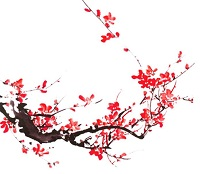
\includegraphics[keepaspectratio=true,scale=0.7]{flower.jpg}}%
    %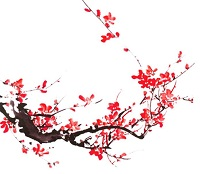
\includegraphics[keepaspectratio=true,scale=0.7]{flower.jpg}%
    \end{figure}%
}
  
\title{\Huge\textsf{夢梅館校本《金瓶梅詞話》}}
\author{蘭陵笑笑生原著\\\kaishu{臺山梅節挺秀校訂}\\\kaishu{金城陳少卿鈔閱}}

\date{}

\newcommand\mydot[1]{\scalebox{#1}{.}}
\renewcommand\cftdot{\mydot{2}}
\renewcommand\cftdotsep{3}
%\renewcommand\cftpartnumwidth{6em}
\renewcommand{\cftchapleader}{\hspace{0.2em}{\cftdotfill{\cftdotsep}}}
%\renewcommand{\cftpnumalign}{l}

%control the right margin of toc-dots:
\makeatletter
\def\@pnumwidth{3.2em}
\makeatother

\begin{document}
\maketitle

\pagestyle{headings}
\pagenumbering{zhdig}
\includepdf[pages={1},fitpaper=false]{tst.pdf}

\cleardoublepage
\tableofcontents
\pdfbookmark{\contentsname}{toc}
%prevent the 1st page of TOC generate foot page number:
\addtocontents{toc}{\protect\thispagestyle{empty}}
%\mainmatter

\pagenumbering{zhdig}
\chapter*{夢梅館校本《金瓶梅詞話》前言}
\addcontentsline{toc}{chapter}{夢梅館校本《金瓶梅詞話》前言}
\markboth{夢梅館校本《金瓶梅詞話》前言}{夢梅館校本《金瓶梅詞話》前言}


《金瓶梅詞話》是中國著名的古典長篇白話小説,也是最具爭論性的小説。自誕生以來,貶之者詆為「市諢之極穢者」,「當急投秦火」{\innerzhushi(明薛岡·天爵堂筆餘)};讚之者譽為「偉大的寫實小説」{\innerzhushi(鄭振鐸·談金瓶梅詞話)},「同時説部,無以上之」{\innerzhushi(魯迅·中國小説史略)}。其實,除去書中一些不雅的性描寫,《金瓶梅詞話》無疑是中國文學寶庫中之奇珍,與《水滸傳》、《紅樓夢》屬同一水平的作品。《金瓶梅》接枝自《水滸》,《紅樓夢》脱胎於《金瓶》;《水滸傳》寫江湖,《金瓶梅》寫市井,《紅樓夢》寫上層貴族,均曲盡其妙。《金瓶梅詞話》的文學地位,亦居於二者之間。

《金瓶梅》的作者,在文學史上至今仍是個謎。欣欣子序雖有「蘭陵笑笑生作金瓶梅傳」的説法,真實姓名與生平事迹均語焉不詳,且亦不見早期抄閱者著錄。後人指為王世貞、李開先、賈三近、屠隆等等,皆缺乏可靠證據。從本書的題旨、内容、取材、叙述結構和語言特徵看,應屬大衆消費性通俗文學,以平話為主體,穿插演唱流行曲。其作者是書會才人一類中下層知識分子,可能與流傳久遠的「羅公(貫中)書會」有某種關係。現存今本詞話,應為民間説書藝人的底本,有的學者甚至認為是「耳錄」{\innerzhushi(傅憎享·金瓶梅隱語揭秘)}。

《金瓶梅》借北宋年號名色,刻劃明代人情世態,開創中國古典長篇小説寫實的傳統。小説講述在明季商品經濟新潮中,一位破落户市棍,欺壓良善,結交勢要,官商通吃,飛黄驣達,享受榮華富貴,最后縱欲身亡的故事。書中的清河,當是運河沿岸一個城鎮。據書中稱淮安、清江浦為「淮上」,稱揚州為「下州」,稱淮河為「南河」,生活場景接近南清河的淮揚地區。《金瓶梅詞話》最初大概就由打談的在淮安、揚州、臨清、濟寧等繁榮、富庶的運河大碼頭上説唱,後來也傳至運河南端的蘇州和杭州{\innerzhushi(明張岱·陶庵夢憶·不繫園)}。聽衆多為客商、船夫、手藝人和市民。

《金瓶梅詞話》借樹開花,從《水滸》武松打虎故事直接切入,開頭有五、六回文字摭自《水滸》,其成書上限不能早於現存百回本《忠義水滸傳》的定型和刊行。書中寫官哥、李瓶兒、西門慶之喪,用的十二個日、月干支,均隆慶五年八月到六年二月的干支;第六十八回提到的「南河南徙」,始於萬暦五年閠八月,此可視為詞話成書的上限{\innerzhushi(梅節·金瓶梅成書的上限、金瓶梅成書於萬曆的新材料)}。大概公元十六世紀末葉、萬曆二十年或稍后,詞話一些不足本已在文人圈子中傳抄。當時如王宇泰、董其昌、袁宏道、王百榖、文在茲、丘志充、謝肇淛、袁中道、沈德符等均有過錄本。在輾轉傳抄過程中,開始形成兩種本子,一為原民間藝人的十卷本,書名《金瓶梅詞話》,有欣欣子序。一為經文士改編的二十卷本,書名《金瓶梅》,有東吴弄珠客序和廿公跋。十卷本《金瓶梅詞話》雖更接近藝人原本,它的刊行却在文人改編的二十卷本《金瓶梅》之後。現存之《新鎸綉像批評金瓶梅》,是這個二十卷本的第二代刻本{\innerzhushi(梅節·新刻金瓶梅詞話後出考)}。

二十卷本在萬曆末、天啓初刊行後風行一時,書林人士見有利可圖,乃梓行十卷本《金瓶梅詞話》。因所據底本也缺五十三至五十七回,乃採二十卷本由陋儒續撰的「這五回」頂補,并錄入二十卷本之弄珠客序、廿公跋以作招徕。十卷本《詞話》因底本訛誤太甚,可讀性差,梓行後并未引起注意,社會上流行的依然是二十卷本,包括後來有張竹坡評的第一奇書本。《詞話》在清初尚有人提及,以後即寂然無聞。一九三二年在山西發現的《新刻金瓶梅詞話》,已屬海内孤本。其後在日本倒發現兩部,一藏日光山輪王寺慈眼堂,一藏德山毛利栖息堂。另京都大學有殘本二十三回,完整者七回。日本兩部《詞話》除栖息堂本第五回末頁曾换版外,與中土本同為一刻。

東土本保持《新刻金瓶梅詞話》素潔的原貌;中土本則有後人的朱筆校改與批語,全書朱墨燦然。一九三三年,馬廉以「古佚小説刊行會」名義,醵資將中土本影印一百零四套{\innerzhushi(魯歌·簡説金瓶梅的幾種版本)}。因錢不够,未能兩色套印,只用單色,朱改變墨改,效果極差。以後中國大陸即據此影印本複印和排印,造成失真。一九六三年,日本大安株式會社據彼邦兩部補配,影印配本《金瓶梅詞話》,稱「日本大安本」。一九七八年,臺北聨經出版事業有限公司按照原藏北京圖書館、現存臺北故宫博物院中土本之原尺寸大小出版朱墨二色套印本。但聨經用作底本的不是原刻,而是傅斯年所藏的古佚小説本,複印經「整理後影印」{\innerzhushi(聨經本金瓶梅詞話·出版説明)},雖糾正古佚小説本據原刻本上朱批改正文的錯誤,墨改部分却未改正(可能没有發現),因此并不徹底。

《金瓶梅》過去被目為淫書,因為它自然主義的反映主人翁西門慶的淫行。從書中一些色情描寫的間歇地重覆出現看,顯然是編撰者為吸引下層聽衆所加添的有味作料。如所周知,《金瓶梅》誕生的時代,是淫風熾盛的明季。遠的不説,萬曆以前幾個皇帝,朱厚照(正德)是「屬皮匠的,縫著的就上」,最後死於豹房。朱厚熜(嘉靖)求丹方,講采補,服紅丸,淫幼女,陶仲文即以方術膺三孤、封恭誠伯。朱戴垕(隆慶)積年服春藥,弄至虛陽舉發,「晝夜不仆」,無法視朝。當時抗倭名將譚綸,一代名相张居正,均以服丹方御女致斃{\innerzhushi(明沈德符·萬曆野獲編·佞倖)}。上行下效,民間則流行淫器、淫藥,浮蕩子弟相率「養龜」。據明末清初佚名作者《如夢錄》記載,明季開封有七家性商店(淫店),都開在撫按諸署附近,專售「廣(景)東人事」、「房中技術」,能「助老扶幼」,「走馬、乌鬚」。在這樣淫靡的社會風氣下,像《金瓶梅詞話》這種大衆消費性通俗文學,為迎合聽衆口味,穿插一些葷笑話、性故事,實不足為怪。何况《金瓶梅》與其他專鋪叙床笫的淫書根本不同,它的一些性描寫只是作為書中人物感官生活的一部分,雖有誇張成分,仍属人欲的範圍。也正因為如此,通過《詞話》的暴露,人们可看到在過去那個時代的男人的性心理,看到女性的卑下和屈辱,也看到人性不那麽可愛的一面。如果把這些文字删去,作品將是残缺的,而且更會引起讀者的好奇,效果適得其反。我们提倡青年人可以先看如《三國演義》、《水滸傳》、《西游記》、《紅樓夢》這些古典文學作品,待心智更成熟,再看《金瓶梅》,也許較為合適。

筆者從八十年代中從事詞話的整理和校點,旨在為讀者提供一個可讀的、較少錯誤的、接近原著的本子。選擇以日本大安本为底本,覆以北京圖書館藏中土本,校以日本内閣文庫和北京大學之《新刻綉像批評金瓶梅》、在茲堂本和崇經堂本之《皋鶴堂批評第一奇書金瓶梅》、并先後参考鄭振鐸、施蟄存、劉本棟、增你智、戴鴻森、白維國卜鍵諸本,兼吸收姚靈犀、魏子雲、陳詔、李申、張惠英、張鴻魁、傅憎享、魯歌等專家研究成果,進行校訂。一九八七年完成第一次校訂,出版《全校本金瓶梅詞話》;一九九三年完成第二次校訂,出版《重校本金瓶梅詞話》一九九九年完成第三次校訂,出版影印《夢梅館定本金瓶梅詞話》手抄本。詳細情况可参閱拙作《金瓶梅詞話的版本與文本——金瓶梅詞話校讀記代序》,这裏不再重覆。

本書在校點过程中,曾得到许多學者和專家的幫助。王修齡、許桂林、馮统一諸先生曾参加全校本校點工作。王先生初校了三十五回至七十回,許先生協助校點了後二十回及書中有關星相部分;馮先生協助校點書中詞曲。陳詔、黄霖兩位先生為重校本作了簡明註釋;蔡敦勇先生對詞曲進行了覆校。陳少卿先生花了三年時間,工楷抄閱三校定本,協助出版《夢梅館定本金瓶梅詞話》手抄影印本。我在此謹向他們,以及對本書的校點出版給予支持和鼓勵的海内外師友,表示由衷的感謝。自己深知,由於寡學淺識,本書在校勘與整理方面都不免存在許多錯誤和不足之處,這只好留待後人來糾正及完善了。

\begin{quotation}
\begin{flushright}

\nopagebreak 前言脱稿於丙寅除夜,刊於全校本與\\重校本。
癸未暮春改定於青衣夢梅館

\end{flushright}
\end{quotation}

\setcounter{footnote}{0}


\chapter*{金瓶梅詞話序}
\addcontentsline{toc}{chapter}{欣欣子《金瓶梅詞話序》}
\markboth{\titlename}{金瓶梅詞話序}


竊謂蘭陵笑笑生作《金瓶梅傳》,寄意於時俗,蓋有謂也。人有七情,憂鬱為甚。上智之士,與化俱生,霧散而氷裂,是故不必言矣。次焉者,亦知以理自排,不使為累。惟下焉者,既不能了於心胸,又無詩書道腴可以撥遣,然則不致於坐病者幾希!吾友笑笑生為此,爰罄平日所蘊者,著斯傳,凡一百囘。其中語句新奇,膾炙人口。無非明人倫、戒淫奔、分淑慝、化善惡,知盛衰消長之機,取報應輪迴之事,如在目前;始終如脈絡貫通,如萬絲迎風而不亂也。使觀者庶幾可以一哂而忘憂也。其中未免語涉俚俗,氣含脂粉。余則曰:不然。《關雎》之作,楽而不淫,哀而不傷。富與貴,人之所慕也,鮮有不至於淫者;哀與怨,人之所惡也,鮮有不至於傷者。吾嘗觀前代騷人,如盧景暉之《剪燈新話》、元微之之《鶯鶯傳》、趙君弼之《效顰集》、羅貫中之《水滸傳》、丘瓊山之《鍾情麗集》、盧梅湖之《懷春雅集》、周靜軒之《秉燭清談》,其後《如意傳》、《于湖記》,其間語句文確,讀者往往不能暢懷,不至終篇而掩棄之矣。此一傳者,雖市井之常談,閨房之碎語,使三尺童子聞之,如飫天漿而拔鯨牙,洞洞然易曉。雖不比古之集理趣,文墨綽有可觀。其它關繋世道風化,懲戒善惡,滌慮洗心,不無小補。譬如房中之事,人皆好之,人非堯舜聖賢,鮮不為所耽。富貴善良,人皆惡之,是以搖動人心,蕩其素志。觀其高堂大廈,雲窗霧閣,何深沉也;金屏綉褥,何羙麗也;鬢雲斜軃,春酥滿胸,何嬋娟也;雄鳳雌凰迭舞,何慇懃也;錦衣玉食,何侈費也;佳人才子,嘲風咏月,何綢繆也;鷄舌含香,唾圓流玉,何溢度也;一雙玉腕綰復綰,兩隻金蓮顛倒顛,何猛浪也。旣其樂矣,然楽極必悲生:如離别之機將興,憔悴之容必見者,所不能免也;折梅逢驛使,尺素寄魚書,所不能無也;患難迫切之中,顛沛流離之頃,所不能脫也;陷命於刀劔,所不能逃也;陽有王法,幽有鬼神,所不能逭也。至於淫人妻子,妻子淫人,祸因惡積,福緣善慶,種種皆不出循環之機。故天有春夏秋冬,人有悲歡離合,莫怪其然也。合天時者,遠則子孫悠久,近則安享終身;逆天時者,身名罹喪,祸不旋踵。人之䖏世,雖不出乎世運代謝,然不經凶祸,不蒙耻辱者,亦幸矣。吾故曰:笑笑生作此傳者,蓋有所謂也。

\begin{quotation}\begin{flushright}欣欣子書於明賢里之軒。\end{flushright}\end{quotation}


\chapter*{跋}
\addcontentsline{toc}{chapter}{廿公《跋》}
\markboth{跋}{跋}
\thispagestyle{empty}

《金瓶梅》,傳為世廟時一鉅公寓言,蓋有所刺也。然曲盡人間醜態,其亦先師不删鄭衛之旨乎?中間䖏處埋伏因果,作者亦大慈悲矣。今後流行此書,功德無量矣。不知者竟目為淫書,不惟不知作者之旨,併亦寃却流行者之心矣!特為白之。

\begin{quotation}\begin{flushright}廿公書。\end{flushright}\end{quotation}


\chapter*{金瓶梅序}
\addcontentsline{toc}{chapter}{東吴弄珠客《金瓶梅序》}
\markboth{\titlename}{金瓶梅序}


《金瓶梅》,穢書也。袁石公亟稱之,亦自寄其牢騷耳,非有取於《金瓶梅》也。然作者亦自有意,蓋為世戒,非為世勸也。如諸婦多矣,而獨以潘金蓮李瓶兒春梅命名者,亦楚《檮杌》之意也。蓋金蓮以姦死,瓶兒以孽死,春梅以淫死,較諸婦為更慘耳。借西門慶以描畫世之大凈,應伯爵以描畫世之小醜,諸淫婦以描畫世之丑婆凈婆,令人讀之汗下。蓋為世戒,非為世勸也。余嘗曰:讀《金瓶梅》而生憐憫心者,菩薩也;生畏懼心者,君子也;生歡喜心者,小人也;生效法心者,乃禽獸耳。余友人褚孝秀,偕一少年同赴歌舞之筵,衍至〈霸王夜宴〉,少年垂涎曰:「男兒何可不如此!」孝秀曰:「也只為這烏江設此一着耳。」同座聞之,歎為有道之言。若有人識得此意,方許他讀《金瓶梅》也。不然,石公幾為導淫宣慾之尤矣!奉勸世人,勿為西門慶之後車可也。

\begin{quotation}\begin{flushright}萬曆丁巳季冬東吴弄珠客漫書於金閶道中。\end{flushright}\end{quotation}


\chapter*{新鐫金瓶梅詞話}
\addcontentsline{toc}{chapter}{新刻金瓶梅詞話·詞曰·四貪詞}
\markboth{\titlename}{新刻金瓶梅詞話·詞曰·四貪詞}


\section*{詞曰}

\begin{myquote0}
閬苑瀛洲,金谷陵樓,筭不如茅舍清幽。野花綉地,莫也風流。也宜春,也宜夏,也宜秋。

酒熟堪あ,客至須留,更無榮無辱無憂。退閒一步,着甚來由?但倦時眠,渴時飲,醉時謳。

短短横牆,矮矮疎窓,忔い兒小小池塘。高低疊峯,綠水邊傍。也有些風,有些月,有些凉。

日用家常,竹几藤床,靠眼前水色山光。客來無酒,清話何妨?但細烹茶,熱烘盞,淺澆湯。

水竹之居,吾愛吾盧,石磷磷床砌堦除。軒窓隨意,小巧䂓模。卻也清幽,也瀟灑,也寬舒。

懶散無拘,此等何如:倚闌干臨水觀魚。風花雪月,贏得功夫,好炷心香,說些話,讀些書。

淨掃塵埃,惜耳蒼苔,任門前紅葉鋪堦。也堪圖畫,還也奇哉!有數株松,數竿竹,數枝梅。

花木栽培,取次教開,明朝事天自安排。知他富貴幾時來?且優遊,且隨分,且開懷。
\end{myquote0}

\newpage\section*{四貪詞}
%\addcontentsline{toc}{chapter}{四貪詞}
%\markboth{\titlename}{四貪詞}

\hspace*{1em}酒

\begin{myquote0}
酒損精神破喪家,語言無狀鬧喧譁。疎親慢友多由你,背義忘恩盡是他。

切須戒,飲流霞。若能依此實無差。失卻萬事皆因此,今後逄賔只待茶。
\end{myquote0}

\hspace*{1em}色

\begin{myquote0}
休愛綠髩羙朱顔,少貪紅粉翠花鈿。損身害命多嬌態,傾國傾城色更鮮。

莫戀此,養丹田。人能寡慾壽長年。従今罷卻閒風月,紙帳梅花獨自眠。
\end{myquote0}

\hspace*{1em}財

\begin{myquote0}
錢帛金珠籠内收,若非公道少貪求。親朋道義因財失,父子懷情為利休。

急縮手,且抽頭。免使身心晝夜愁。兒孫自有兒孫福,莫與兒孫作遠憂。
\end{myquote0}

\hspace*{1em}氣

\begin{myquote0}
莫使強梁逞技能,揮拳捰袖弄精神。一時怒發無明火,到後憂煎祸及身。

莫太過,免災迍。勸君凡事放寬情。合撒手時須撒手,得饒人處且饒人。
\end{myquote0}

\part*{夢梅館校本《金瓶梅詞話》卷之一}
\addcontentsline{toc}{part}{夢梅館校本《金瓶梅詞話》卷之一}


\includepdf[pages={1,2},fitpaper=false]{tst.pdf}
\chapter*{第一囬 \\景陽岡武松打虎 潘金蓮嫌夫賣風月}
\addcontentsline{toc}{chapter}{第一囬 景陽岡武松打虎 潘金蓮嫌夫賣風月}
\markboth{\titlename}{第一囬 景陽岡武松打虎 潘金蓮嫌夫賣風月}


詞曰:

\begin{myquote}
丈夫隻手把吴鈎,欲斬萬人頭。如何鐵石,打成心性,却為花柔?

請看項籍並劉季,一怒使人愁。只因撞着,虞姬戚氏,豪傑都休!
\end{myquote}

此一隻詞兒,單說着「情」、「色」二字,乃一體一用。故色絢於目,情感於心,情色相生,心目相視。亘古及今,仁人君子,弗能忘之。晋人云:情之所鍾,正在我輩。如磁石吸鐵,隔礙潛通。無情之物尚爾,何况為人,终日在情色中做活計者耶?詞兒「丈夫隻手把吴鈎」,吴鈎,乃古劔也。古有干將、莫邪、太阿、吴鈎、魚腸、屬鏤之名。言丈夫心腸如鐵石,氣槪貫虹蜺,不免屈志於女人。

題起當時西楚霸王,姓項名籍,單名羽字。因秦始皇無道,南修五嶺,北築長城,東填大海,西建阿房,並吞六國,坑儒焚典。因與漢王劉邦,單名季字,時二人起兵,席捲三秦,滅了秦國,指鴻溝為界,平分天下。因用范增之謀,連敗漢王七十二陣。只因寵着一個婦人,名喚虞姬,有傾城之色,載於軍中,朝夕不離。一旦被韓信所敗,夜走陰陵,爲追兵所逼。霸王欲向江東取救,因捨虞姬不得,又聞四面皆楚歌,事發,嘆曰:「力拔山兮氣蓋世,時不利兮騅不逝,騅不逝兮可奈何,虞兮虞兮奈若何!」歌畢,淚下數行。虞姬曰:「大王莫非以賤妾之故,有廢軍中大事?」霸王曰:「不然,吾與汝不忍相捨故耳!況汝這般容色,劉邦乃酒色之君,必見汝而納之。」虞姬泣曰:「妾寜以義死,不以苟生。」遂請王之寳劍,自刎而死。霸王因大慟,尋以自剄。史官有詩嘆曰:

\begin{myquote}
「拔山力盡霸圖隳,倚劍空歌不逝騅。

明月滿營天似水,那堪囬首别虞姬。」
\end{myquote}

那漢王劉邦,原是泗上亭長,提三尺劍,う碭山斬白蛇起手,二年亡秦,五年滅楚,掙成天下。只因也是寵着個婦人,名喚戚氏夫人,所生一子,名趙王如意。因被吕后妒害,心甚不安。一日,高祖有疾,乃枕戚夫人腿而臥。夫人哭曰:「陛下萬歲後,妾母子何所托?」帝曰:「不難。吾明日出朝,廢太子而立爾子,意下如何?」戚夫人乃收淚謝恩。吕后聞之,密召張良謀計。良擧薦商山四皓,下來辅佐太子。一日,同太子入朝。高祖見四人鬚鬢皎白,衣冠甚偉,各問姓名。一名東園公,一名綺里季,一名夏黄公,一名甪里先生。因大驚問:「朕昔求聘諸公,如何不至,今日乃從吾兒所遊?」四皓答曰:「太子乃守成之主也。」高祖聞之,愀然不悦。比及四皓出殿,乃召戚夫人指示之曰:「我欲廢太子,况彼四人輔佐,羽翼已成,卒難搖動矣。」戚夫人遂哭泣不止。帝乃作歌以解之:

\begin{myquote}
「鴻鵠高飛兮,一擧千里。羽翼已就兮,横絶四海。横絶四海兮,又可奈何?雖有矰繳兮,尚安所施!」
\end{myquote}

歌訖,後遂不果立趙王矣。高祖崩世,吕后酒酖殺趙王如意,人彘了戚夫人,以除其心中之患。

詩人评此二君,评到個去處,說劉項者,固當世之英雄,不免爲二婦人以屈其志氣。雖然,妻之視妾,名分雖殊,而戚氏之祸,尤慘於虞姬。然則妾婦之道,以色事其丈夫,而欲保全首領於牖下,難矣。觀此二君,豈不是「撞着虞姬戚氏,豪傑都休」?有詩爲證:

\begin{myquote}
劉項佳人絕可憐,英雄無策庇嬋娟。

戚姬葬處君知否?不及虞姬有墓田。
\end{myquote}

說話的如今只愛説這情色二字做甚?故士矜才則德薄,女衒色則情放。若乃持盈慎滿,則為端士淑女。豈有殺身之祸?今古皆然,貴賤一般。如今這一本書,乃虎中羙女,後引出一個風情故事來。一個好色的婦女,因與個破落户相通,日日追歡,朝朝迷戀。後不免屍横刀下,命染黄泉,永不得着綺穿羅,再不能施朱傅粉。靜而思之,着甚來由?況這婦人他死有甚事?貪他的,斷送了堂堂六尺之軀;愛他的,丢了潑天關産業。驚動了東平府,大鬧了清河縣。端的不知誰家婦女?誰的妻小?後日乞何人占用?死於何人之手?正是:說時華嶽山峰歪,道破黄河水逆流!

話說宋徽宗皇帝政和年間,朝中寵信高楊童蔡四個奸臣,以致天下大亂,黎民失業,百姓倒懸,四方盗賊蜂起。罡星下生人間,攪亂大宋花花世界,四處反了四大寇。那四大寇?山東宋江、淮西王慶、河北田虎、江南方臘。皆轟州劫縣,放火殺人,僭稱王號。惟有宋江替天行道,專報不平,殺天下贜官汚吏豪惡刁民。

那時山東陽谷縣,有一人姓武,名植,排行大郎。有個嫡親同胞兄弟,名喚武松。其人身長七尺,膀闊三停。自幼有膂力,學得一手好槍棒。他的哥哥武大,生的身不滿三尺,爲人懦弱,又頭腦濁蠢可笑。平日本分,不惹是非。因時遭荒饉,將祖房兒賣了,與兄弟分居,搬移在清河縣居住。這武松因酒醉打了童樞密,單身獨自逃在滄州横海郡小旋風柴進莊上,——他那裏招攬天下英雄豪傑,仗義疎财,人號他做「小孟嘗君」柴大官人,乃是周朝柴世宗嫡派子孫,——那裏躲逃。柴進因見武松是一條好漢,收攬在莊上。不想武松就害起瘧疾來,住了一年有餘,因思想哥哥武大,告辭歸家。在路上行了幾日,來到清河縣地方。

那時山東界上,有一座景陽崗,山中有一隻弔睛白額虎,食得路絶人稀。官司杖限獵户,擒捉此虎。崗子路上兩邊都有榜文,可敎過往經商,結夥成群於巳午未三個時辰過崗,其餘不許過崗。這武松聽了,呵呵大笑。就在路旁酒店内喫了幾碗酒。壯着膽,横拖着防身梢棒,踉踉蹌蹌大扠步走上崗來。不半里之地,見一座山神廟,門首貼着一張印信榜文。武松看時,上面寫道:

\begin{myquote}[\markfont]
「景陽崗上,有一隻大蟲,近來傷人甚多。現今立限各鄉里正並獵户人等,打捕住時,官給賞銀三十兩。如有過往客商人等,可於巳午未三個時辰,結夥過崗。其餘時分,及單身客旅,白日不許過崗,恐被傷害性命不便。各宜知悉。」
\end{myquote}

武松喝道:「怕甚麽鳥!且只顧上崗去,看有甚大蟲。」武松將棒綰在脅下,一步步上那崗來。囘看那日色,漸漸下山。此正是十月間天氣,日短夜長,容易得晚。武松走了一會,酒力發作,遠遠望見亂樹林子,直奔過樹林子來。見一塊光撻撻的大青臥牛石,把那棒倚在一邊,放翻身體,恰待要睡,但見青天忽然起一陣狂風,看那風時,但見:

\begin{myquote}
無形無影透人懷,四季能吹萬物開,

就地撮將黄葉去,入山推出白雲來。
\end{myquote}

原來雲生從龍,風生從虎。那一陣風過處,只聽得亂樹背後黄葉刷刷的響,撲地一聲,跳出一隻弔睛白額斑斕猛虎來,猶如牛來大。武松見了,叫聲「阿呀」時,從青石上翻身下來,便提梢棒在手,閃在青石背後。那大蟲又饑又渴,把兩隻爪在地上跑了一跑,打了個歡翅,將那條尾剪了又剪,半空中猛如一個焦霹靂,滿山滿嶺盡皆振響。這武松被那一驚,把肚中酒都變做冷汗出了。說時遲,那時快,武松見大蟲撲來,只一閃,閃在大蟲背後。原來猛虎項短,回頭看人較難,便把前爪搭在地下,把腰胯一伸,掀將起來;武松只一躲,躲在側邊。大蟲見掀他不着,吼了一聲,把山崗也振動。把這鐵棒也似虎尾倒豎起來,只一剪,武松却又閃過一邊。原來虎傷人,只是一撲、一掀、一剪,三般捉不着時,氣力已自没了一半。武松見虎没力,翻身囘來,雙手輪起梢棒,盡平生氣力,只一棒,——只聽得一聲響,簌簌地將那樹枝帶葉打將下來。原來不曾打着大蟲,正打在樹枝上,磕磕把那條棒折做兩截,只拿一半在手裏。這武松心中,也有幾分慌了。那虎便咆哮性發,剪尾弄風起來,向武松又只一撲,撲將來。武松一跳,卻跳回十步遠。那大蟲撲不着武松,把前爪搭在武松面前。武松將半截棒丢在一邊,乘勢向前,兩隻手撾住大蟲頂花皮,使力只一按。那虎急要掙扎,早沒了氣力。武松儘力撾定那虎,那裏肯放鬆。一面把隻脚望虎面上眼睛裏只顧亂踢。那虎咆哮,把身底下扒起兩堆黄泥,做了一個土坑。武松按在坑裏,騰出右手,提起拳頭來只顧狠打。儘平生氣力,不消半歇兒時辰,把那大蟲打死,躺卧着卻似一個綿布袋,動不得了。有古風一篇,單道景陽崗武松打虎。但見:

\begin{myquote}
景陽崗頭風正狂,萬里陰雲埋日光。

焰焰滿川紅日赤,紛紛遍地草皆黄。

觸目晚霞掛林藪,侵人冷霧滿穹蒼。

忽聞一聲霹靂響,山腰飛出獸中王;

昂頭踴躍逞牙爪,谷裏獐鹿皆奔降。

山中狐兔潛踪跡,澗内獐猿驚且慌。

卞莊見後魂魄散,存孝遇時心膽亡。

清河壯士酒未醒,忽在崗頭偶相迎。

上下尋人虎饑渴,撞着猙獰來撲人。

虎來撲人似山倒,人去迎虎如巖傾。

臂腕落時墜飛砲,爪牙撾處幾泥坑。

拳頭脚尖如雨點,淋漓兩手鮮血染。

穢汚腥風滿松林,散亂毛鬚墜山崦。

近看千鈞勢未休,遠觀八面威風減。

身横野草錦斑消,緊閉雙睛光不閃。
\end{myquote}
	
當下這隻猛虎,被武松沒頓飯之間,一頓拳脚,打的動不得了。使的這漢子口裏兀自氣喘不息。武松放了手,來松樹邊尋那打折的梢棒。只怕大蟲不死,向身上又打了十數下,那大蟲氣都没了。武松尋思:「我就勢把這大蟲拖下崗子去。」就血泊中雙手來提時,那裏提得動?原來使盡了氣力,手脚都酥軟了。武松正坐在石上歇息,只聽草坡裏刷剌剌響。武松口中不言,心下驚恐:「天色已黑了,倘或又跳出一個大蟲來,我却怎生鬦得過他?」剛言未畢,只見坡下鑽出兩隻大蟲來,唬得武松大驚道:「阿呀,今番我死也!」只見那兩個大蟲於面前直立起來。武松定睛看時,却是個人:把虎皮縫做衣裳,頭上帶着虎磕腦。那兩人手裏各拿着一條五股鋼叉,見了武松倒頭便拜,說道:「壯士,你是人也,神也?端的喫了㺀え心、豹子肝、獅子腿,膽倒包了身軀!不然,如何獨自一個,天色漸晚,又沒器械,打死這個傷人大蟲?我們在此觀看多時了。端的壯士,高姓大名?」武松道:「我行不更名,坐不改姓,自我便是陽谷縣人氏,姓武名松,排行第二。」因問:「你兩個是甚麽人?」那兩個道:「不瞞壯士說,我們是本處打獵户。因為崗前這隻虎,夜夜出來,傷人極多。只我們獵户也折了七八個,過路客人不計其數。本縣知縣相公,着落我們衆獵户限日捕捉,得獲時,賞銀三十兩;不獲時,定限喫拷。叵耐這業畜勢大,難近得他,誰敢向前?我們只和數十鄉夫在此,遠遠地安下窝弓藥箭等他。正在這裏埋伏,却見你大剌剌從崗子上走來,三拳兩脚,和大蟲敵鬦,把大蟲登時打死了。未知壯士身上有多少力!俺衆人把大蟲綣了,請壯士下崗,往本縣去見知縣相公,討賞去來。」於是衆鄉夫獵户,約凑有七八十人,先把死大蟲擡在前面,將一個兜轎擡了武松,逕投本䖏一個上户家。那上户里正都在莊前迎接,把這大蟲扛在草庭上。却有本縣里老,都來相探,問了武松姓名。因把打虎一節,說了一遍。衆人道:「真乃英雄好漢!」那衆獵户先把野味將來,與武松把盞,喫得大醉。打掃客房,武松歇息。

到天明,里老先去縣裏報知。一面合具虎牀,安排花紅軟轎,迎送武松到縣衙前。清河縣知縣使人來接到縣内廳上。那滿縣人民聽得說一個壯士打死了景陽崗上大蟲,迎賀將來,盡皆出來觀看,哄動了那個縣治。武松到廳上下了轎,扛着大蟲在廳前。知縣看了武松這般模様,心中自忖道:「不恁地,怎打得這個猛虎?」便唤武松上廳來。參見畢。將打虎首尾,訴說了一遍。兩邊官吏,都驚獃了。知縣就廳上賜了幾盃酒,將庫中衆上户出納的賞錢三十兩,就賜與武松。武松禀道:「小人托賴相公的福蔭,偶然僥倖打死了這個大蟲。非小人之能,如何敢受這三十兩賞賜?衆獵户因這畜生,受了相公許多責罰。何不就把這賞給散與衆人去?也顯相公恩沾,小人義氣。」知縣道:「旣是如此,任從壯士處分。」武松就把這三十兩賞錢,在廳上俵散與衆獵户去了。知縣見他仁德忠厚,又是一條好漢,有心要擡擧他,便道:「你雖是陽谷縣的人氏,與我這清河縣只在咫尺。我今日就參你在我這縣裏做個巡捕的都頭,專一河東水西擒拿盗賊,你意下如何?」武松跪謝道:「若蒙恩相擡擧,小人終身受賜。」知縣隨即喚押司立了文案,當日便參武松做了巡捕都頭。衆里正大户,都來與武松作賀慶喜,連連誇官,喫了三五日酒。武松正要陽谷縣找尋哥哥,不料又在清河縣做了都頭。一日在街上閑遊,喜不自勝。傳得東平一府兩縣,皆知武松之名。有詩為證:

\begin{myquote}
壯士英雄藝略芳,挺身直上景陽崗。

醉來打死山中虎,自此聲名播四方。
\end{myquote}
	
按下武松,單表武大。自從與兄弟分居之後,因時遭荒饉,搬移在清河縣紫石街賃房居住。人見他為人懦弱,模様猥衰,起了他個渾名,叫做「三寸丁、谷樹皮」。俗語言其身上粗糙,頭臉窄狹故也。以此人見他這般軟弱樸實,都欺負他。武大並無生氣,常時迴避便了。看官聽說:世上惟有人心最歹,軟的又欺,惡的又怕;太剛則折,太柔則廢。古人有幾句格言說的好:

\begin{myquote}
柔軟立身之本,剛強惹祸之胎。無爭無競是賢才,虧我些兒何礙?青史幾場春夢,紅塵多少奇才。不須計較巧安排,守分而今見在。
\end{myquote}

且說武大終日挑擔子出去街上,賣炊餅度日。不幸把渾家故了,丢下個女孩兒,年方十二歲,名喚迎兒。爺兒兩個過活,那消半年光景,又消折了資本,移在大街坊張大户家臨街房居住,依舊做買賣。張宅家下人見他本分,常看顧他,照顧他炊餅。閑時在他舖中坐,武大無不奉承。因此張宅家下人個個都歡喜,在大户面前,一力與他說方便,因此大户連房錢也不問武大要。

這張大户家有萬貫家財,百間房産,年約六旬之上,身邊寸男尺女皆無。媽媽余氏,主家嚴厲,房中並無清秀使女。一日,大户拍胸嘆了一口氣。媽媽問道:「你田産豐盛,資財充足,閑中何故嘆氣?」大户道:「我許大年紀,又無兒女,雖有家財,終無大用。」媽媽道:「旣然如此說,我教媒人替你買兩個使女,早晚習學彈唱,服侍你便了。」大户心中大喜,謝了媽媽。過了幾時,媽媽果然敎媒人來,與大户買了兩個使女,一個叫做潘金蓮,一個喚做白玉蓮。這潘金蓮却是南門外潘裁的女兒,排行六姐。因他自幼生得有些顔色,纏得一雙好小脚兒,因此小名金蓮。父親死了,做娘的因度日不過,從九歲賣在王招宣府裏,習學彈唱,就會描眉畫眼,傅粉施朱,梳一個纏髻兒,着一件扣身衫兒,做張做勢,喬模喬樣。況他本性機變伶俐,不過十五,就會描鸞刺綉,品竹彈絲,又會一手琵琶。後王招宣死了,潘媽媽爭將出來,三十兩銀子轉賣與張大户家,與玉蓮同時進門。在大户家習學彈唱,金蓮學琵琶,玉蓮學箏。玉蓮亦年方二八,乃是樂户人家女子,生得白凈,小字玉蓮。這兩個同房歇臥。主家婆余氏初時甚是擡擧二人,不令上鍋,聊備洒掃,與他金銀首飾,粧束身子。後日不料白玉蓮死了,止落下金蓮一人,長成一十八歲,出落的臉襯桃花,不紅不白;眉彎新月,又細又彎。張大户每要收他,只怕主家婆利害,不得手。一日,主家婆鄰家赴席不在,大户暗把金蓮喚至房中,遂收用了。正是:羙玉無瑕,一朝損壞。珍珠何日,再得完全?

大户自從收用金蓮之後,不覺身上添了四五件病症。端的那五件?第一,腰便添疼;第二,眼便添淚;第三,耳便添聾;第四,鼻便添涕;第五,尿便添滴。還有一樁兒不可說,白日間只是打盹,到晚來噴㖒也無數。後主家婆頗知其事,與大户嚷駡了數日,將金蓮甚是苦打。大户知不容此女,却賭氣倒賠房奩,要尋嫁得一個相應的人家。大户家下人,都說武大忠厚,現無妻小,又住着宅内房兒,堪可與他。這大户早晚還要看覷此女,因此不要武大一文錢,白白的嫁與他為妻。這武大自従娶的金蓮來家,大户甚是看顧他。若武大沒本錢做炊餅,大户私與他銀兩:與他做本錢。武大若挑擔兒出去,大户候無人,便踅入房中與金蓮廝會。武大雖一時撞見,亦不敢聲言。朝來暮往,如此也有幾時。忽一日,大户得患陰寒病症,嗚呼哀哉死了。主家婆察知其事,怒令家童將金蓮武大即時趕出,不容在房子裏住。武大不免又尋紫石街西王皇親房子,賃内外兩間居住,依舊賣炊餅。原來金蓮自從嫁武大,見他一味老實,人物猥衰,甚是憎嫌,常與他合氣。抱怨大户:「普天世界斷生了男子,何故將奴嫁與這樣個貨!每日牽着不走,打着倒腿的,只是一味お酒。着緊處却是錐扎也不動。奴端的那世裏晦氣,卻嫁了他!是好苦也!」常無人處唱個〔山坡羊〕爲證:

\begin{myquote}
「想當初,姻緣錯配,奴把他當男兒漢看覷。不是奴自己誇獎,他烏鴉怎配鸞鳳對?奴真金子埋在土裏,他是塊高麗銅,怎與俺金色比!他本是塊頑石,有甚福抱着我羊脂玉體?好似糞土上長出靈芝。奈何?隨他怎樣,倒底奴心不羙!聽知:奴是塊金磚,怎比泥土基!」
\end{myquote}

看官聽說:但凡世上婦女,若自己有些顔色,所禀伶俐,配個好男子便罷了,若是武大這般,雖好煞,也未免有幾分憎嫌。自古佳人才子相凑着的少,買金偏撞不着賣金的。武大每日自挑炊餅擔兒出去賣,到晚方歸。婦人在家,别無事幹,一日三餐喫了飯,打扮光鮮,只在門前簾兒下站着,常把眉目嘲人,雙睛傳意。左右街坊,有幾個奸詐浮浪子弟,睃見了武大這個老婆,打扮油樣,沾風惹草,被這干人在街上撒謎語,往來嘲戯唱叫:「這一塊好羊肉,如何落在狗口裏!」人人只知武大是個懦弱之人,却不知他娶得這個婆娘在屋裏,風流伶俐,諸般都好,為頭的一件好偷漢子。有詩為證:

\begin{myquote}
金蓮容貌更堪題,笑蹙春山八字眉。

若遇風流清子弟,等閑雲雨便偸期。
\end{myquote}

這婦人每日打發武大出門,只在簾子下嗑瓜子兒,一徑把那一對小金蓮故露出來,勾引的這夥人日逐在門前彈胡博詞、扠兒機,口裏油似滑言語,無般不說出來。因此武大在紫石街住不牢,又要往别䖏搬移,與老婆商議。婦人道:「賊混沌,不曉事的!你賃人家房住,淺房淺屋,可知有小人囉唣!不如凑幾兩銀子,看相應的典上他兩間住,卻也氣概些,免受人欺負。你是個男子漢,倒擺布不開,常敎老娘受氣!」武大道:「我那裏有錢典房?」婦人道:「呸!濁材料!把奴的釵梳凑辦了去,有何難處?過後有了,再治不遲。」武大聽了老婆這般說,當下凑了十數兩銀子,典得縣門前樓,上下兩層,四間房屋居住。第二層是樓,兩個小小院落,甚是乾凈。

武大自從搬到縣西街上來,照舊賣炊餅。一日,街上所過,見數隊纓鎗,鑼鼓喧天,花紅軟轎,簇擁着一個人,卻是他嫡親兄弟武松。因在景陽崗打死了大蟲,知縣相公擡擧他,新陞做了巡捕都頭。街上里老人等作賀他,送他下處去。卻被武大撞見,一手扯住,叫道:「兄弟,你今日做了都頭,怎不看顧我?」武松囬頭,見是哥哥。二人相會,兄弟大喜,一面邀請到家中,讓至樓上坐。房裏喚出金蓮來,與武松相見。因說道:「前日景陽岡打死了大蟲的,便是你小叔。今新充了都頭,是我一母同胞兄弟。」那婦人叉手向前,便道:「叔叔萬福!」武松施禮,倒身下拜。婦人扶住武松道:「叔叔請起,折殺奴家。」武松道:「嫂嫂受禮。」兩個相讓了一囬,都平磕了頭,起來。少頃,小女迎兒拿茶,二人喫了。武松見婦人十分妖嬈,只把頭來低着。不多時,武大安排酒飯,管待武松。說話中間,武大下樓買酒菜去了,丢下婦人,獨自在樓上陪武松坐的。看了武松身材凜凜,相貌堂堂,身上恰似有千百斤氣力。——不然,如何打得那大蟲?心裏尋思道:「一母所生的兄弟,又這般長大,人物壯健,奴若嫁得這個,胡亂也罷了。你看我家那身不滿尺的『丁樹』,三分似人,七分似鬼。奴那世裏遭瘟,直到如今!據看武松又好氣力,何不教他搬來我家住?誰想這段姻緣,卻在這裏!」那婦人一面臉上堆下笑來,問道:「叔叔,你如今在那裏居住?每日飯食,誰人整理?」武松道:「武二新充了都頭,逐日答應上司,别䖏住不方便,胡亂在縣前尋了個下處,每日撥兩個土兵服事做飯。」婦人道:「叔叔何不搬來家裏住,省的在縣前土兵服事,做飯腌臢。一家裏住,早晚要些湯水喫時,也方便些。就是奴家親自安排與叔叔喫,也乾凈。」武松道:「深謝嫂嫂。」婦人又道:「莫不别䖏有嬸嬸,可請來廝會也。」武松道:「武二並不曾婚娶。」婦人道:「叔叔青春多少?」武松道:「虚度二十八歲。」婦人道:「原來叔叔倒長奴三歲。叔叔今番従那裏來?」武松道:「在滄州住了一年有餘,只想哥哥在舊房居住,不想搬在這裏!」婦人道:「一言難盡。自從嫁得你哥哥,喫他忒善了,被人欺負,纔得到這裏。若似叔叔這般雄壯,誰敢道個不字。」武松道:「家兄從來本分,不似武松撒潑。」婦人笑道:「怎的顛倒說?常言人無剛強,安身不牢。奴家平生快性,看不上這樣三打不囘頭,四打連身轉的人。」有詩為證,詩曰:

\begin{myquote}
叔嫂萍踪得偶逢,嬌嬈偏逞秀儀容。

私心便欲成歡會,暗把邪言釣武松。
\end{myquote}

原來這婦人甚是言語撇清。武松道:「家兄不惹祸,免嫂嫂憂心。」二人只在樓上説話未了,只見武大買了些肉菜果餅歸來,放在廚下。走上樓來呌道:「大嫂,你且下來安排則個。」那婦人應道:「你看那不曉事的!叔叔在此,無人陪侍,卻敎我撇了下去?」武松道:「嫂嫂請方便。」婦人道:「何不去間壁,請王乾娘來安排便了。只是這般不見便?」武大便自去央了間壁王婆子來,安排端正,都拿上樓來,擺在桌子上,無非是些魚肉、果菜、點心之類,隨即盪上酒來。武大教婦人坐了主位,武松對席,武大打横,三人坐下,把酒來斟。武大篩酒在各人面前。那婦人拿起酒來道:「叔叔休怪,没甚管待,請盃兒水酒。」武松道:「感謝嫂嫂,休這般說。」武大只顧上下篩酒,那裏來閑事。那婦人笑容可掬,滿口兒呌:「叔叔,怎的肉果兒也不揀一筯兒?」揀好的遞將過來。武松是個直性漢子,只把做親嫂嫂相待。誰知這婦人是個使女出身,慣會小意兒;亦不想這婦人一片引人心。那武大又是善弱的人,那裏會管待人。婦人陪武松喫了幾盃酒,一雙眼只看着武松身上。武松乞他看不過,只低了頭不理他。喫了一歇,酒闌了,便起身。武大道:「二哥,没事再喫幾盃兒去。」武松道:「生受!我再來望哥哥嫂嫂罷。」都送下樓來。出的門外,婦人便道:「叔叔是必上心,搬來家裏住!若是不搬來,俺兩口兒也喫别人笑話。親兄弟,難比别人,與我們爭口氣,也是好處!」武松道:「既是吾嫂厚意,今晚有些行李,便取來。」婦人道:「叔叔是必記心者,奴這裏專候!」正是:滿前野意無人識,幾點碧桃春自開。有詩為證:

\begin{myquote}
可怪金蓮用意深,包藏淫行蕩春心。

武松正大原難犯,耿耿清名抵萬金。
\end{myquote}

當日這婦人情意十分殷勤。卻說武松到縣前客店内,收拾行李鋪蓋,敎土兵挑了,引到哥家。那婦人見了,強如拾了金寶一般歡喜。旋打掃一間房,與武松安頓停當。武松吩咐土兵囬去,當晚就在哥家宿歇。次日早起,婦人也慌忙起來,與他燒湯淨面。武松梳洗裹幘,出門去縣裏畫卯,婦人道:「叔叔畫了卯,早些來家喫飯,休去别處喫了。」武松應諾。到縣裏畫卯已畢,伺候了一早晨,囬到家中。那婦人又早齊齊整整,安排下飯,三口兒同喫了飯。婦人雙手便捧一盃茶來,遞與武松。武松道:「教嫂嫂生受,武松寢食不安!明日縣裏撥個土兵來使喚。」那婦人連聲叫道:「叔叔,卻怎生這般計較?自家骨肉,又不服事了別人!雖然有這小丫頭迎兒,奴家見他拿東拿西蹀里蹀斜,也不靠他。就是撥了土兵來,那廝上鍋上竈不乾凈,奴眼裏也看不上這等人。」武松道:「恁的,却生受嫂嫂了!」有詩為證:

\begin{myquote}
武松儀表甚搊搜,嫂嫂淫心不可收。

籠絡歸來家裏住,要同雲雨會風流。
\end{myquote}

話休絮煩。自従武松搬來哥家裏住,取些銀子出來與武大,教買餅饊茶果,請那兩邊鄰舍。衆憐舍都鬦分子,來與武松人情。武大又安排了囬席,都不在話下。過了數日,武松取出一疋彩色緞子,與嫂嫂做衣服。那婦人堆下笑來,便道:「叔叔,如何使得!旣然賜與,奴家不敢推辭,只得接了。」道個萬福。自此武松只在哥家歇宿。武大依前上街挑賣炊餅。武松每日自去縣裏承差應事,不論歸遲歸早,婦人炖羹炖飯,歡天喜地服事武松。武松倒安身不得:那婦人時常把些言語來撥他,武松是個硬心的直漢。

有話即長,無話即短,不覺過了一月有餘,看看十一月天氣,連日朔風緊起。只見四下彤雲密布,又早紛紛揚揚,飛下一天瑞雪來。但見: 

\begin{myquote}
萬里彤雪密佈,空中祥瑞飄簾,瓊花片片舞前簷。剡溪當此際,濡滯子猷船。頃刻樓臺都壓倒,江山銀色相連。飛鹽撒粉漫連天,當時呂蒙正,窑内嗟無錢。
\end{myquote}

當日這雪直下到一更時分,却似銀粧世界,玉碾乾坤。次日,武松早去縣裏畫卯,直到日中未歸。武大被婦人早趕出去做買賣,央及間壁王婆,買了些酒肉;去武松房裏,簇了一盆炭火。心裏自想道:「我今日着實撩鬦他一鬦,不怕他不動情!」那婦人獨自冷冷清清立在簾兒下,望見武松正在雪裏踏着那亂瓊碎玉歸來。婦人推起簾子,迎着笑道:「叔叔寒冷。」武松道:「感謝嫂嫂掛心!」入得門來,便把毡笠兒除將下來,那婦人將手去接。武松道:「不勞嫂嫂,生受!」自把雪來拂了,掛在壁子上。隨即解了纏帶,脱了身上鸚哥綠紵絲衲襖,入房内搭了。那婦人便道:「奴等了一早晨,叔叔怎的不歸來喫早飯?」武松道:「早間有一相識請我喫飯了,却纔又有一個作盃,我不耐煩,一直走到家來。」婦人道:「旣恁的,請叔叔向火。」武松道:「正好。」便脫了油靴,換了一雙襪子,穿了暖鞋,掇條凳子,自近火盆邊坐的。那婦人早令迎兒把前門上了閂,後門也關了。却搬些煮酒菜蔬入房裏來,擺在桌子上。武松問道:「哥哥那裏去了?」婦人道:「你哥哥每日自出去做些買賣,我和叔叔自喫三盃。」武松道:「一發等哥來家,喫也不遲。」婦人道:「那裏等的他!」說猶未了,只見迎兒小女早煖了一注酒來。武松道:「不必嫂嫂費心,待武二自斟。」婦人也掇一條凳子,近火邊坐了。桌上擺着盃盤,婦人拿盞酒擎在手裏,看着武松:「叔叔滿飲此盃!」武松接過酒去,一飲而盡。那婦人又篩一盃來,說道:「天氣寒冷,叔叔飲個成雙的盞兒。」武松道:「嫂嫂自飲。」接來又一飲而盡。武松却篩一盃酒,遞與婦人。婦人接過酒來呷了,却拿注子再斟酒,放在武松面前。那婦人一徑將酥胸微露,雲鬟半軃,臉上堆下笑來,說道:「我聽得人説,叔叔在縣前街上養着個唱的,有這話麽?」武松道:「嫂嫂休聽別人胡說,我武二従來不是這等人!」婦人道:「我不信,只怕叔叔口頭不似心頭。」武松道:「嫂嫂不信時,只問哥哥就是了。」婦人道:「呵呀,你休說,他那裏曉得甚麽?如在醉生夢死一般。他若知道時,不賣炊餅了。叔叔且請一盃!」連篩了三四盃飲過。那婦人也有三盃酒落肚,烘動春心,那裏按納得住?慾心如火,只把閑話來說。武松也知了八九分,自己只把頭來低了,却不來兜攬。婦人起身去盪酒,武松自在房内,却拿火筯簇火。婦人良久煖了一注子酒,來到房裏,一隻手拿着注子,一隻手便去武松肩上只一捏,說道:「叔叔,只穿這些衣服,不寒冷麽?」武松已有五七分不自在,也不理他。婦人見他不應,劈手便來奪火筯,口裏道:「叔叔你不會簇火,我與你撥火!只要一似火盆來熱便好。」武松有八九分焦躁,只不做聲。這婦人也不看武松焦躁,便丢下火筯,卻篩一盞酒來,自呷了一口,剩下大半盞酒,看着武松道:「你若有心,喫我這半盃兒殘酒。」乞武松劈手奪過來,潑在地下。說道:「嫂嫂,不要恁的不識羞耻!」把手只一推,爭些兒把婦人推了一跤。武松睜起眼來說道:「武二是個頂天立地的噙齒戴髮的男子漢,不是那等敗壞風俗傷人倫的猪狗!嫂嫂休要這般不識羞耻,為此等的勾當,倘有些風吹草動,我武二眼裏認的是嫂嫂,拳頭却不認的是嫂嫂!再來休要如此所爲。」婦人喫他幾句,搶得通紅了面皮,便叫迎兒收拾了碟盞家伙。口裏指着說道:「我自作耍子,不值得便當真起來,好不識人敬!」收了家伙,自往廚下去了。有詩爲證:

\begin{myquote}
潑賤操心太不良,貪淫無耻壞綱常。

席間尚且求雲雨,反被都頭駡一場。
\end{myquote}

這婦人見勾搭武松不動,反被他搶白了一場好的。武松自在房中氣忿忿的,自己尋思。天色却早申牌時分,武大挑着擔兒大雪裏歸來。推開門,放下擔兒,進的房來,見婦人一雙眼哭的紅紅的,便問道:「你和誰鬧來?」婦人道:「都是你這不不爭氣的,教外人來欺負我!」武大道:「誰敢來欺負你?」婦人道:「情知是誰!爭奈武二那廝。我見他大雪裏歸來,好意安排些酒飯與他喫,他見前後没人,便把言語來調戲我。便是迎兒眼見,我不賴他!」武大道:「我兄弟不是這等人,從來老實。休要高聲,乞鄰舍聽見笑話!」武大撇了婦人,便來武松房裏。叫道:「二哥,你不曾喫點心,我和你喫些個。」武松只不做聲。尋思了半晌,脱了絲鞋,依舊穿上油臘靴,着了上蓋,戴上毡笠兒。一面繋纏帶,一面出大門。武大叫道:「二哥,你那裏去?」也不答,一直只顧去了。武大囘到房内,問婦人道:「我呌他,又不應,只顧往縣前那條路去了。正不知怎的了!」婦人罵道:「賊混沌蟲!有甚難見䖏?那廝羞了,没臉兒見你,走了出去。我猜他一定呌個人來搬行李,不要在這裏住。却不道你留他!」武大道:「他搬了去,須乞别人笑話。」婦人罵道:「混沌魍魎,他來調戲我,到不乞别人笑話?你要,便自和他過去,我却做不的這樣人。你與了我一紙休書,你自留他便了!」武大那裏再敢開口,被這婦人倒數罵了一頓。

正在家兩口兒絮聒,只見武松引了個土兵,拿着條扁擔,徑來房内,收拾行李便出門。武大走出來,呌道:「二哥,做甚麽便搬了去?」武松道:「哥哥不要問,說起來裝你的幌子。只由我自去便了!」武大那裏再敢問備細,由武松搬了出去。那婦人在裏面喃喃呐呐駡道:「却也好!只道是親難轉債,人只知道一個兄弟做了都頭怎的養活了哥嫂,却不知反來嚼咬人!正是花木瓜,空好看。搬了去,倒謝天地,且得冤家離眼前。」武大見老婆這般言語,不知怎的了,心中只是放它不下。

自從武松搬去縣前客店宿歇,武大自依前上街賣炊餅。本待要去縣前尋兄弟說話,却被這婦人千叮萬囑,吩咐教不要去兜攬他,因此武大不敢去尋武松。有詩為證:

\begin{myquote}
雨意雲情不遂謀,心中誰信起戈矛。

生將武二搬離去,骨肉翻令作寇讐!
\end{myquote}

畢竟未知後來何如,且聽下囘分解。


\includepdf[pages={3,4},fitpaper=false]{tst.pdf}
\chapter*{第二囬 \\西門慶簾下遇金蓮 王婆子貪賄說風情}
\addcontentsline{toc}{chapter}{第二囬 西門慶簾下遇金蓮 王婆子貪賄說風情}
\markboth{第二囬 西門慶簾下遇金蓮 王婆子貪賄說風情}{第二囬 西門慶簾下遇金蓮 王婆子貪賄說風情}
\thispagestyle{empty}

\begin{myquote}
月老姻缘配未真,金蓮賣俏逞花容。
只因月下星前意,惹起門旁簾外心。

王婆誘財施巧計,鄆哥賣果被嫌嗔。
那知後日蕭牆祸,血濺屏幃滿地紅。
\end{myquote}

話説武松自從搬離哥家,撚指不覺雪晴,過了十數日光景。

却說本縣知縣,自從到任以來,却得二年有餘,賺得許多金銀。要使一心腹人,送上東京親眷處收寄,三年任滿朝覲,打點上司。一來却怕路上小人,須得一個有力量的人去方好。猛可想起都頭武松:「須得此人英雄膽力,方了得此事。」當日就喚武松到衙内商議道:「我有個親戚,在東京城内做官,姓朱名勔,現做殿前太尉之職。要送一擔禮物,捎封書去問安。只恐途中不好行,須得你去方可。你休推辭辛苦,囬來我自重賞你。」武松應道:「小人得蒙恩相擡擧,安敢推辭?旣蒙差遣,只得便去。小人自來也不曾到東京,就那裏觀光上國景緻,走一遭,也是恩相擡擧。」知縣大喜,賞了武松三盃酒,十兩路費,不在話下。

且說武松領了知縣的言語,出的縣門來,到下處呌個土兵,却來街上買了一瓶酒並菜蔬之類,逕到武大家。武大恰街上囬來,見武松在門前坐地,教土兵去廚下安排。那婦人餘情不斷,見武松把將酒食來,心中自思:「莫不這廝思想我了?不然却又囬來!那廝一定強我不過,我且慢慢問他。」婦人便上樓去,重勻粉面,再挽雲鬟,換了些顔色衣服穿了,來到門前迎接武松。婦人拜道:「叔叔!不知怎的錯見了,好幾日並不上門,教奴心裏沒理會處。每日教你哥哥去縣裏尋叔叔陪話,歸來只説沒尋處。今日再喜得叔叔來家。没事壞鈔做甚麽!」武松道:「武二有句話,特來要和哥哥說知。」婦人道:「旣如此,請樓上坐。」

三個人來到樓上,武松讓哥嫂上首坐了,他便掇杌子打横。土兵擺上酒來,熱下飯,一齊拿上來。武松勸哥嫂喫。婦人便把眼來睃武松,武松只顧喫酒。酒至數巡,武松問迎兒討副勸盃,叫土兵篩一盃酒,拿在手裏,看着武大道:「大哥在上,武二今日蒙知縣相公差往東京幹事,明日便要起程。多是兩三個月,少是一個月便囬。有句話特來和你說:你從來為人懦弱,我不在家,恐怕外人來欺負。假如你每日賣十扇籠炊餅,你從明日為始,只做五扇籠炊餅出去賣。每日遲出早歸,不要和人喫酒。歸家便下了簾子,早閉門,省了多少是非口舌。若是有人欺負你,不要和他爭執,待我囬來,自和他理論。大哥,你依我時,滿飲此盃!」武大接了酒道:「我兄弟見得是,我都依你説。」喫過了一盃,武松再斟第二盞酒,對那婦人說道:「嫂嫂是個精細的人,不必要武松多說。我的哥哥,為人質朴,全靠嫂嫂做主。常言表壯不如裏壯。嫂嫂把得家定,我哥哥煩惱做甚麽?豈不聞古人云:籬牢犬不入!」那婦人聽了這幾句話,一點紅從耳畔起,須臾紫漒了面皮,指着武大駡道:「你這個混沌東西,有甚言語在别人䖏說,來欺負老娘!我是個不帶頭巾的男子漢,叮叮噹噹響的婆娘,拳頭上也立的人,胳膊上走得馬,人面上行的人,不是那腲膿血搠不出來鱉老婆!自従嫁了武大,眞個螻蟻不敢入屋裏來,有甚麽「籬笆不牢犬兒鑽得入來」?你休胡言亂語,一句句都要下落。丢下塊磚兒,一個個也要着地!」武松笑道:「若得嫂嫂這般做主,最好。只要心口相應。却不應心頭不似口頭。旣然如此,我武松都記得嫂嫂說的話了,請過此盃!」那婦人一手推開酒盞,一直跑下樓來,走到半胡梯上,發話道:「旣是你聰明伶俐,却不道長嫂如母?我初嫁武大時,不曾聽得有甚小叔。那裏走得來,是親不是親,便要做喬家公!自是老娘晦氣了,偏撞着這許多鳥事!」一面哭下樓去了。有詩為證:

\begin{myquote}
苦口良言諫勸多,金蓮懷恨起風波。

自家惶愧難存坐,氣殺英雄小二哥。
\end{myquote}

那婦人做出許多喬張致來。武大武松喫了幾杯酒,坐不住,都下的樓來,弟兄洒淚而别。武大道:「兄弟去了,早早囬來,和你相見。」武松道:「哥哥,你便不做買賣也罷,只在家裏坐的。盤纏兄弟自差人送與你。」臨行,武松又吩咐道:「哥哥,我的言語,休要忘了,在家仔細門户!」武大道:「理會得了。」武松辭了武大,回到縣前下處,收拾行裝並防身器械。次日,領了知縣禮物,金銀馱垜,討了脚程,起身上路,往東京去了。不題。

只說武大,自從兄弟武松説了去,整整乞那婆娘駡了三四日。武大忍氣吞聲,由他自罵,只依兄弟言語,每日只做一半炊餅出去,未晚便囬家。歇了擔兒,先便去除了簾子,關上大門,却來屋裏動彈。那婦人看了這般,心内焦躁起來,罵道:「不識時濁物!我倒不曾見日頭在半天裏,便把牢門關了,也喫鄰舍家笑話,說我家怎生禁鬼!聽信你兄弟說空生有卵鳥嘴,也不怕别人笑恥!」武大道:「由他笑也罷,我兄弟說的是好話,省了多少是非。」被婦人噦在臉上道:「呸!濁東西,你是個男子漢,自不做主,却聽別人調遣!」武大搖手道:「由他,我兄弟説的是金石之語!」原來武松去後,武大每日只是晏出早歸,到家便關門。那婦人氣生氣死,和他合了幾場氣。落後鬧慣了,自此婦人約莫武大歸來時分,先自去收簾子,關上大門。武大見了,心裏自也暗喜,尋思道:「恁的却不好?」有詩爲證:

\begin{myquote}
慎事關門幷早歸,眼前恩愛隔崔嵬。

春心一點如絲亂,任鎖牢籠總是虚。
\end{myquote}

白駒過隙,日月攛梭,纔見梅開臘底,又早天氣囬陽。一日,三月春光明媚時分,金蓮打扮光鮮,單等武大出門,就在門前簾下站立,——約莫將及他歸來時分,便下了簾子,自去房内坐的。一日,也是合當有事,却有一個人從簾子下走過來。自古没巧不成話,姻緣合當凑着:婦人正手裏拿着叉竿放簾子,忽被一陣風將叉竿刮倒,婦人手擎不牢,不端不正,却打在那人頭巾上。婦人便慌忙陪笑,把眼看那人,也有二十五六年紀,生得十分博浪:

\begin{myquote}
頭上戴着纓子帽兒,金玲瓏簪兒,金井玉欄杆圈兒;長腰身,穿綠羅褶兒;脚下細結底陳橋鞋兒,清水布襪兒;腿上勒着兩扇玄色挑絲護膝兒;手裏搖着洒金川扇兒,越顯出張生般龐兒,潘安的貌兒,——可意的人兒,風風流流従簾子下丢與奴個眼色兒。
\end{myquote}

這個人被叉竿打在頭上,便立住了脚。待要發作時,囬過臉來看,却不想是個羙貌妖嬈的婦人。但見他:

\begin{myquote}
黑鬒鬒賽鴉翎的鬢兒,翠彎彎的新月的眉兒,清泠泠杏子眼兒,香噴噴櫻桃口兒,直隆隆瓊瑤鼻兒,粉濃濃紅豔腮兒,嬌滴滴銀盆臉兒,輕嬝嬝花朵身兒,玉纖纖葱枝手兒,一捻捻楊柳腰兒,軟濃濃白麵臍肚兒,窄多多尖趫脚兒,肉奶奶胸兒,白生生腿兒;更有一件緊揪揪、紅縐縐、白鮮鮮、黑裀裀,正不知是什麽東西!
\end{myquote}

觀不盡這婦人容貌,且看他怎生打扮?但見:

\begin{myquote}
頭上戴着黑油油頭髮䯼髻,四面上貼着飛金。一逕裏墊出香雲一結,周圍小簪兒齊插。六鬢斜插一朶並頭花,排草梳兒後押。難描八字彎彎柳葉,襯在腮兩朶桃花。玲瓏墜兒最堪誇,露賽玉酥胸無價。毛青布大袖衫兒褶兒又短,襯湘裙碾絹綾紗。通花汗巾兒袖中兒邊搭剌,香袋兒身邊低掛。抹胸兒重重紐扣。褲腿兒臟頭垂下。往下看:尖趫趫金蓮小脚,雲頭巧緝山牙;老鴉鞋兒白綾高底,步香塵偏襯登踏。紅紗膝褲扣鶯花,行坐處風吹裙袴。口兒裏常噴出異香蘭麝,櫻桃初笑臉生花。人見了魂飛魄散,賣弄殺偏俏的寃家!
\end{myquote}

那人見了,先自酥了半邊,那怒氣早已鑽入爪哇國去了,變做笑吟吟臉兒。這婦人情知不是,叉手望他深深拜了一拜,說道:「奴家一時被風失手,誤中官人,休怪。」那人一面把手整頭巾,一面把腰曲着地,還喏道:「不妨!娘子請方便。」却被這間壁住的賣茶王婆子看見。那婆子笑道:「兀的誰家大官人打這屋簷下過?打的正好!」那人笑道:「倒是我的不是,一時衝撞,娘子休怪!」婦人答道:「官人不要見責!」那人又笑着大大地唱個喏,囬應道:「小人不敢!」那一雙積年招花惹草,慣覷風情的賊眼,不離這婦人身上。臨去也囬頭了七八遍,方一直搖搖擺擺,遮着扇兒去了。有诗為證:

\begin{myquote}
風日清和漫出遊,偶従簾下識嬌羞。

只因臨去秋波轉,惹起春心不肯休。
\end{myquote}

當時婦人見了那人生的風流浮浪,語言甜淨,更加幾分留戀:「倒不知此人姓甚名誰,何處居住。他若沒我情意時,臨去也不囬頭七八遍了。不想這段姻緣,却在他身上!」却是在簾下眼巴巴的,看不見那人,方纔收了簾子,關上大門歸房去了。

看官聽説:莫不這人無有家業的?原是清縣一個破落户財主,就縣門前開着個生薬舖。從小兒也是個好浮浪子弟,使得些好拳棒,又會賭博,雙陸象棋,拆白道字,無不通曉。近來發跡有錢,專在縣裏管些公事,與人把攬說事過錢,交通管吏。因此滿縣人都懼怕他。那人複姓西門,單名一個慶字,排行第一,人都叫他做西門大郎。近來發跡有錢,人都稱他做西門大官人。他父母雙亡,兄弟俱無,先頭渾家已早逝,身邊止有一女。新近又娶了清河左衛吴千户之女,填房為繼室。房中也有四五個丫鬟婦女。又常與勾欄裏的李嬌兒打熱,今也娶在家裏。南街子又占着窠子卓二姐,名卓丢兒,包了些時,也娶來家居住。專一嫖風戲月,調占良人婦女。娶到家中,稍不中意,就令媒人賣了;一個月倒在媒人家去二十餘遍。人都不敢惹他。

這西門大官人自從簾下見了那婦人一面,到家尋思道:「好一個雌兒,怎能够得手?」猛然想起那間壁賣茶王婆子來:「堪可如此如此,這般這般。撮合得此事成,我破幾兩銀子謝他,也不值甚的。」於是連飯也不喫,走出街上閑遊,一直逕踅入王婆茶坊裏來,便去裏邊水簾下坐了。王婆笑道:「大官人,却纔唱得好個大肥喏!」西門慶道:「乾娘,你且來,我問你:間壁這個雌兒是誰的娘子?」王婆道:「他是閻羅大王的妹子,五道將軍的女兒,問他怎的?」西門慶說:「我和你説正話,休取笑。」王婆道:「大官人怎的不認的?他老公便是縣前賣熟食的。」西門慶道:「莫不是賣棗糕徐三的老婆?」王婆搖手道:「不是!若是他,也是一對兒。大官人再猜!」西門慶道:「敢是賣餶飿的李三娘子兒?」王婆搖手道:「不是!若是他,倒是一雙。」西門慶道:「莫不是花胳膊劉小二的婆兒?」王婆大笑道:「不是!若是他時,又是一對兒。大官人再猜!」西門慶道:「乾娘,我其實猜不着了。」王婆哈哈笑道:「好敎大官人得知了罷,笑一聲。他的蓋老,便是街上賣炊餅的武大郎!」西門慶聽了,跌脚笑道:「莫不是人叫他三寸丁谷樹皮的武大郎麽?」王婆道:「正是他。」西門慶聽了,叫起苦來,説道:「好一塊羊肉,怎生落在狗口裏!」王婆道:「便是這般苦事。自古駿馬却馱癡漢走,羙妻常伴拙夫眠。月下老偏這等配合!」西門慶道:「乾娘,我少你多少茶果錢?」王婆道:「不多。由他,歇些時却算不妨。」西門慶又道:「你兒子王潮,跟誰出去了?」王婆道:「說不的,跟了一個淮上客人,至今不歸,又不知死活。」西門慶道:「却不叫他跟我?那孩子倒乖覺伶俐!」王婆道:「若得大官人擡擧他時,十分之好。」西門慶道:「待他歸來,却再計較。」說畢,作謝起身去了。約莫未及兩個時辰,又踅將來王婆門首簾邊坐的,朝着武大門前。半歇,王婆出來道:「大官人,喫個梅湯?」西門慶道:「最好,多加些酸味兒。」王婆做了個梅湯,雙手遞與西門慶,喫了,將盞子放下。西門慶道:「乾娘,你這梅湯做得好,有多少在屋裏?」王婆笑道:「老身做了一世媒,那討得一個在屋裏?」西門慶笑道:「我問你這梅湯,你却說做媒,差了多少!」王婆道:「老身只聽得大官人問這媒做得好,老身只道說做媒。」西門慶道:「乾娘,你旣是撮合山,也與我做頭媒!說頭好親事,我自重重謝你。」王婆道:「看這大官人作戲!你宅上大娘子得知,老婆子這臉上怎吃得那等刮子!」西門慶道:「我家大娘子最好性格。現今也有幾個身邊人在家,只是沒一個中得我意的。你有這般好的,與我主張一個,便來說也不妨。若是囬頭人兒也好,只是要中得我意。」王婆道:「前日有一個倒好,只怕大官人不要。」西門慶道:「若是好時,與我說成了,我自重謝你。」王婆道:「生的十二分人才,只是年紀大些。」西門慶道:「自古半老佳人可共,便差一兩歲也不打緊。真個多少年紀?」王婆子道:「那娘子是丁亥生,屬猪的,交新年恰九十三歲了。」西門慶笑道:「你看這風婆子,只是扯着風臉取笑!」說畢,西門慶笑了起身去。

看看天色晚了,王婆恰纔點上燈來,正要關門。只見西門慶又踅將來,俓去簾子底下,那凳子上坐了,朝着武大門前,只顧將眼睃望。王婆道:「大官人,喫個和合湯?」西門慶道:「最好,乾娘放甜些。」王婆連忙取一鍾來,與西門慶喫了。坐到晚夕,起身道:「乾娘,記了帳目,明日一發還錢。」王婆道:「由他,伏惟安置,來日再請過访。」西門慶笑了去。到家甚是寢食不安,一片心只在婦人身上。當晚無話。

次日清晨,王婆恰纔開門,把眼看外時,只見西門慶又早在街前來囬踅走。王婆道:「這刷子踅得緊。你看我着些甜糖,抹在這廝鼻子上,教他舐不着!那廝會討縣裏人便益,且敎他來老娘手裏納些財鈔,賺他幾貫風流錢使。」原來這開茶坊的王婆子,也不是守本分的。便是積年通殷勤,做媒婆,做賣婆,做牙婆,又會收小的,也會抱腰,又善放刁。還有一件不可說,䯼髻上着綠,陽臘灌腦袋。端的看不出這婆子的本事來!但見:

\begin{myquote}
開言欺陸賈,出口勝隨何。只憑說六國唇鎗,全仗話三齊舌劍:隻鸞孤鳳,霎時間交仗成雙;寡婦鰥男,一席話搬唆擺對。解使三重門内女,遮麽九級殿中僊。玉皇殿上侍香金童,把臂拖來;王母宫中傳言玉女,攔腰抱住。略施奸計,使阿羅漢抱住比丘尼;纔用機關,教李天王摟定鬼子母。甜言說誘,男如封陟也生心;軟語調和,女似麻姑須亂性。藏頭露尾,攛掇淑女害相思;送暖偸寒,調弄嫦娥偸漢子。這婆子,端的慣調風月巧安排,常在公門遭鬦毆。
\end{myquote}

這婆子正開門,在茶局子裏整理茶鍋。張見西門慶踅過幾遍,奔入茶局子水簾下,對着武大門首,不住把眼只望簾子裏瞧。王婆只推不看見,只顧在茶局子内搧火,不出來問茶。西門慶叫道:「乾娘,點兩盃茶來我喫。」王婆應道:「大官人來了?連日少見,且請坐。」不多時,便濃濃點兩盞稠茶,放在桌子上。西門慶道:「乾娘,相陪我喫個茶。」王婆哈哈笑道:「我又不是你影射的,緣何陪着你喫茶?」西門慶也笑了。一會,便問:「乾娘,間壁賣的是甚麽?」王婆道:「他家賣的拖煎河漏子、軟巴子肉、翻包着菜肉匾食、餃窝窝、蛤蜊麵,熱盪溫和大辣酥。」西門慶笑道:「你看這風婆子,只是風!」王婆笑道:「我不是風,他家自有親老公!」西門慶道:「我和你説正經話。他家如灋做得好炊餅,我要問他買四五十個,拿的家去。」王婆道:「若要買他炊餅,少間等他街上囬來買,何消上門上户?」西門慶道:「乾娘說的是。」喫了茶,坐了一會,起身去了。

良久,王婆只在茶局裏張時,冷眼張見他在門前,踅過東,看一看,又轉西去,又睃一睃,一連走了七八遍。少頃,逕入茶房裏來。王婆道:「大官人稀行,好幾日不見面了!」西門慶便笑將起來,去身邊摸出一兩一塊銀子,遞與王婆,說道:「乾娘,權且收了做茶錢。」王婆笑道:「何消得許多!」西門慶道:「多者乾娘只顧收着。」婆子暗道:「來了,這刷子當敗。且把銀子收了,到明日與老娘做房錢!」便道:「老身看大官人有些渴,喫個寬煎茶兒如何?」西門慶道:「如何乾娘便猜得着?」婆子道:「有甚難猜處?自古入門休問榮枯事,觀看形容便得知。老身異樣蹺蹊古怪的事不知猜够多少。」西門慶道:「我一件心上的事,乾娘若猜得着時,便輸與你五兩銀子。」王婆笑道:「老身也不消三智五猜,只一智便猜個中節。大官人,你將耳朶來:你這兩日脚步兒勤趕趁得頻,一定是記掛着間壁那個人。我這猜如何?」西門慶笑將起來道:「乾娘端的智賽隨何,機強陸賈。不瞞乾娘說,不知怎的,喫他那日叉簾子時見了一面,恰似收了我三魂六魄的一般,日夜只是放他不下。到家茶飯懶喫,做事没入脚處。不知你會弄手段麽?」王婆哈哈笑道:「老身不瞞大官人說,我家賣茶,呌做鬼打更。三年前六月初三日下大雪那一日,賣了一個泡茶,直到如今不發市,只靠些雜趁養口。」西門慶道:「乾娘,如何叫做雜趂?」王婆笑道:「老身自従三十六歲沒了老公,丢下這個小廝,無得過日子。迎頭兒跟着人說媒,次後攬人家些衣服賣,又與人家抱腰收小的,閑常也會做牽頭,做馬泊六,也會針灸看病,也會做貝戎兒。」西門慶聽了,笑將起來:「我並不知乾娘有如此手段!端的與我說這件事成,便送十兩銀子與你做棺材本。你好敎這雌兒會我一面。」王婆便哈哈笑了。有詩為證:

\begin{myquote}
西門浪子意猖狂,死下功夫戲女娘。

虧殺賣茶王老母,生敎巫女會襄王。
\end{myquote}

畢竟婆子有甚計策說來,要知後項事情,且聽下囬分解。


\includepdf[pages={5,6},fitpaper=false]{tst.pdf}
\chapter*{第三囬 \\王婆定十件挨光計 西門慶茶房戲金蓮}
\addcontentsline{toc}{chapter}{第三囬 王婆定十件挨光計 西門慶茶房戲金蓮}
\markboth{第三囬 王婆定十件挨光計 西門慶茶房戲金蓮}{第三囬 王婆定十件挨光計 西門慶茶房戲金蓮}
\thispagestyle{empty}

\begin{myquote}
色不迷人人自迷,迷他端的受他虧:

精神耗散容顔淺,骨髓焦枯氣力微。

犯着姦情家易散,染成色病薬難醫。

古来饱煖生閑事,祸到頭來總不知。
\end{myquote}

話説西門慶央王婆,一心要會那雌兒一面,便道:「乾娘,你端的與我說這件事成,我便送十兩銀子與你。」王婆道:「大官人,你聽我說,但凡『挨光』的兩個字最難。——怎的是『挨光』?似如今俗呼『偸情』就是了。——要五件事俱全,方纔行的。第一,要潘安的貌;第二,要驢大行貨;第三,要鄧通般有錢;第四,要粧小伏低,就要綿裏針一般軟款忍耐;第五、要閑工夫。此五件喚做『潘驢鄧小閑』,都全了,此事便獲得着。」西門慶道:「實不瞞你說,這五件事我都有。第一件,我的貌雖比不得潘安,也充得過。第二件,我小時在三街兩巷遊串,也曾養得好大龜。第三,我家裏也有幾貫錢財,雖不及鄧通,也頗得過日子。第四,我最忍耐,他便就打我四百頓,休想我囬他一拳。第五,我最有閑工夫。不然,如何來得恁勤?乾娘,你自作成我,完備了時,我自重重謝你!」西門慶當日意已在言表。王婆道:「大官人,你說五件事都全,我知道還有一件事打攪,也都是成不得!」西門慶道:「且說甚麽一件事打攪?」王婆道:「大官人,休怪老身直言,但凡挨光,最難十分。肯使錢到九分九厘,也有難成處。我知你從來慳吝,不肯胡亂便使錢。只這件打攪。」西門慶道:「這個容易,我只聽你言語便了。」王婆道:「若大官人肯使錢時,老身有一條妙計,須教大官人和這雌兒會一面。只不知大官人肯依我麽?」西門慶道:「不揀怎的,我都依你。端的有甚妙計?」王婆笑道:「今日晚了,且囬去,過半年三個月來商量。」西門慶央及道:「乾娘,你休撒科,自作成我則個!恩有重報。」王婆笑哈哈道:「大官人却又慌了。老身這條計,雖然入不得武成王廟,端的強似孫武子敎女兵,十捉八九着。大官人,今日實對你說了罷,這個雌兒來歷,雖然微末出身,却倒百伶百俐,會一手好彈唱。針指女工,百家詞曲,雙陸象棋,無般不知。小名叫做金蓮,娘家姓潘。原是南關外潘裁的女兒,賣在張大户家學彈唱。後因大户年老,打發出來,不要武大一文錢,白白與了他為妻。占用這幾年,武大為人軟弱,每日早出晚歸,只做買賣。這雌兒等閑不出來。老身無事,常過去與他閑坐,他有事亦來請我理會。他也叫我做乾娘。武大這兩日出門早。大官人如幹此事,便買一疋藍紬、一疋白紬、一疋白絹,再用十兩好綿,都把來與老身。老身却走過去,問他借曆日——央及人揀個好日期,叫個裁縫來做送終衣服。他若見我這般來說,揀了日期不肯與我來做時,此事便休了;他若歡天喜地,說『我替你做』,不要我叫裁縫,這光便有一分了。我便請得他來做,就替我裁,這便二分了。他若來做時,午間我却安排些酒食點心,請他喫。他若說不便當,定要將去家中做,此事便休了;他不言語喫了時,這光便有三分了。這一日你也莫來。直到第三日晌午前後,你整整齊齊打扮了來,以咳嗽為號。你在門前叫道:『怎的連日不見王乾娘?我來買盞茶喫。』我便出來請你入房裏坐,喫茶。他若見你,便起身來走了歸去,——難道我扯住他不成?此事便休了;他若見你入來,不動身時,這光便有四分了。坐下時,我便對雌兒說道:『這個便是與我衣料施主的官人,虧殺他!』我便誇大官人許多好䖏,你便賣弄他針指,若是他不來兜攬答應時,此事便休了;他若口裏答應,與你說話時,這光便有五分。我却說道:『難為這位娘子,與我作成出手做。虧殺你兩施主,一個出錢,一個出力。不是老身路歧相央,難得這位娘子在這裏,官人做個主人,替娘子澆澆手。』你便取銀子出來,央我買。若是他便走時,——不成我扯住他?此事便休了;若是不動身時,事務易成,這光便有六分了。我却拿銀子,臨出門時,對他說:『有勞娘子相待官人坐一坐。』他若起身走了家去,——我難道阻擋他?此事便休了;若是他不起身,又好了,這光便有七分了。待我買得東西,擺在桌子上,便說:『娘子,且收拾過生活去,且喫一盃兒酒,難得這官人壞錢。』他不肯和你同桌喫,走了囬去,此事便休了;若是只口裏說要去,却不動身,此事又好了,這光便有八分了。待他喫得酒濃時,正說得入港,我便推道没了酒,再教你買。你便拿銀子,又央我買酒去,並菓子來配酒。我把門拽上,關你和他兩個在屋裏。若焦躁跑了歸去時,此事便休了;他若由我拽上門,不焦躁時,這光便有九分,只欠一分了便完就。這一分倒難。大官人,你在房裏,便着幾句甜話兒說入去,却不可躁爆便去動手動脚,打攪了事。那時我不管你。你先把袖子向桌子上拂落一雙筯下去,只推拾筯,將手去他脚上揑一揑。他若鬧將起來,我自來搭救。此事便休了,再也難成。若是他不做聲時,此事十分光了,他必然有意。這十分光做完備,你怎的謝我?」西門慶聽了大喜道:「雖然上不得凌煙閣,乾娘,你這條計端的絶品好妙計!」王婆道:「却不要忘了許我那十兩銀子!」西門慶道:「便得一片橘皮喫,切莫忘了洞庭湖。這條計,乾娘幾時可行?」王婆道:「亦只今晚來有囬報。我如今趂武大未歸,過去問他借曆日,細細說念他。你快使人送將紬絹綿子來,休要遲了。」西門慶道:「乾娘若完成得這件事,如何敢失信!」於是作别了王婆,離了茶肆,就去街上買了紬絹三疋,並十兩清水好綿。家裏叫了個貼身答應的小廝,名喚玳安,用包袱包了,一直送入王婆家來。王婆歡喜收下,打發小廝囘去。正是:巫山雲雨幾時就?空使襄王築楚臺。有詩為證:

\begin{myquote}
兩意想投似蜜甜,王婆撮合更稀奇。

安排十件挨光計,管取交歡不負期。
\end{myquote}

當下王婆收了紬絹綿子,開了後門,走過武大家來。那婦人接着,請去樓上坐的。王婆道:「娘子怎的這兩日不過貧家喫茶?」那婦人道:「便是我這幾日身子不快,懶去走動。」王婆道:「娘子家裏有曆日,借與老身看一看,要個裁衣的日子。」婦人道:「乾娘裁甚衣服?」王婆道:「便是因老身十病九痛,怕一時有些山高水低,我兒子又不在家。」婦人道:「大哥怎的一向不見?」王婆道:「那廝跟了個客人在外邊,不見個音信囬來,老身日逐躭心不下。」婦人道:「大哥今年多少青春?」王婆道:「那廝十七歲了。」婦人道:「怎的不與他尋個親事?與乾娘也替得手。」王婆道:「因是這等說。家中沒人,待老身東擯西補的來。早晚也替他尋下個兒。等那廝來,却再理會。現如今老身白日黑夜,只發喘咳嗽,身子打碎般睡不倒的只害疼,一時先要預備下送終衣服。難得一個財主官人,常在貧家喫茶。但凡他宅裏看病、買使女、說親,見老身這般本分,大小事兒無不照顧老身。又布施了老身一套送終衣料,紬絹表裏俱全,又有若干好綿,放在家裏一年有餘,不能夠閑做得。今年覺得好生不濟,不想又撞着閏月,趂着兩日倒閑,要做,又被那裁縫勒掯,只推生活忙不肯來做。老身說不得這苦也!」那婦人聽了,笑道:「只怕奴家做得不中意,若是不嫌時,奴這幾日倒閑,出手與乾娘做如何?」那婆子聽了,堆下笑來,說道:「若得娘子貴手做時,老身便死也得好䖏去。久聞娘子好針指,只是不敢來相央。」那婦人道:「這個何妨?旣是許了乾娘,務要與乾娘做了。將曆日去敎人揀個黄道好日,奴便動手。」王婆道:「娘子,休推老身不知!你詩詞百家曲兒内字樣,你不知會了多少,如何叫人看曆日?」婦人微笑道:「奴家自幼失學。」婆子道:「好說,好說!」便取曆日遞與婦人。婦人接在手内,看了一囬道:「明日是破日,後日也不好。直到外後日,方是裁衣日期。」王婆一把手取過歷頭來,掛在牆上,便道:「若得娘子肯與老身做時,就是一點福星,何用選日!老身也曾央人看來,說明日是個破日。老身只道裁衣日可用破日,不忌他!」那婦人道:「歸壽衣服,正用破日便好。」王婆道:「旣是娘子肯作成,老身膽大,只是明日起動娘子到寒家則個。」那婦人道:「不必,將過來做不得?」王婆道:「便是老身也要看娘子做生活,又怕門首没人。」婦人道:「旣是這等說,奴明日飯後過來。」那婆子千恩萬謝,下樓去了,當晚囬覆了西門慶話,約定後日准來。當夜無話。

次日清晨,王婆收拾房内乾凈,預備下針線,安排了茶水,在家等候。且說武大喫了早飯,挑着擔兒自出去了。那婦人把簾兒掛了,吩咐迎兒看家,従後門走過王婆家來。那婆子歡喜無限,接入房裏坐下,便濃濃點一盞胡桃松子泡茶,與婦人喫了。抹得桌子乾凈,便取出那紬絹三疋來。婦人量了長短,裁得完備,縫將起來。婆子看了,口裏不住聲假喝采道:「好手段!老身也活了六七十歲,眼裏真個不曾見這個好針線!」那婦人縫到日中,王婆安排些酒食請他,又下了一筯麵與那婦人喫。再縫一歇,將次晚來,便收拾了生活自歸家去。恰好武大挑擔兒進門,婦人拽開門,下了簾子。武大入屋裏,看見老婆面色微紅,問道:「你那裏來?」婦人應道:「便是間壁乾娘,央我做送終衣服。日中安排了些酒食點心,請我喫。」武大道:「你也不要喫他的纔得,我們也有央及他䖏。他便央你做得衣裳,你便自歸來喫些點心,不值得甚麽,便攪擾他?你明日再去做時,带些錢在身邊,也買些酒食與他囬禮。常言道:遠親不如近鄰,休要失了人情!他若不肯敎你還禮時,你便拿了生活來家,做還與他便了。」有詩為證:

\begin{myquote}
阿母牢籠設計深,大郎愚鹵不知音。

帶錢買酒酬奸詐,却把婆娘白送人。
\end{myquote}

婦人聽了武大言語,當晚無話。次日飯後,武大挑擔兒出去了,王婆便踅過來相請。婦人去到他家房裏,取出生活來,一面縫起。王婆忙點茶來,與他喫了茶。看看縫到日中,那婦人向袖中取出三百文錢來,向王婆說道:「乾娘,奴和你買盞酒喫。」王婆道:「阿呀,那裏有這個道理。老身央及娘子在這裏做生活,如何教娘子倒出錢?婆子的酒食不到的喫傷了哩!」那婦人道:「却是拙夫吩咐奴來。若是乾娘見外時,只是將了家去,做還乾娘便了。」那婆子聽了道:「大郎直恁地曉事!旣然娘子這般說時,老身且收下。」這婆子生怕打攪了事,自又添錢去買好酒好食、希奇果子來,殷勤相待。看官聽說:但凡世上婦人,由你十分精細,被小意兒過縱,十個九個着了道兒。這婆子安排了酒食點心,請那婦人喫了。再縫了一歇,看看晚來,千恩萬謝歸去了。

話休絮煩。第三日早飯後,王婆只張武大出去了,便走過來後門首,叫道:「娘子,老身大膽!」那婦人從樓上應道:「奴却待來也。」兩個廝見了,來到王婆房裏坐下,取過生活來縫。那婆子隨即點盞茶來,兩個喫了。婦人看看縫到晌午前後。

却說西門慶巴不到此日,打選衣帽,齊齊整整,身邊帶着三五兩銀子,手裏拿着洒金川扇兒,搖搖擺擺,逕往紫石街來。到王婆茶坊門首,便咳嗽道:「王乾娘,連日如何不見?」那婆子瞧科,便應道:「兀的誰叫老娘?」西門慶道:「是我。」那婆子趕出來看了,笑道:「我只道是誰,原來是大官人!你來得正好,且請入屋裏去看一看。」把西門慶袖子只一拖,拖進房裏來。看那婦人道:「這個便是與老身衣料施主官人。」西門慶睜眼看着那婦人:雲鬟疊翠,粉面生春;上穿白夏布衫兒,桃紅裙子,藍比甲;正在房裏做衣服。見西門慶過來,便把頭低了。這西門慶連忙向前屈身唱喏。那婦人隨即放下生活,還了萬福。王婆便道:「難得官人與老身緞疋紬絹,放在家一年有餘,不曾做得;虧殺鄰家這位娘子出手與老身做成全了。真個是布機也似針線,縫的又好又密,真個難得!大官人,你過來且看一看。」西門慶把起衣服來看了,一面喝采,口裏道:「這位娘子傳得這等好針指,神僊一般的手段!」那婦人笑道:「官人休笑話。」西門慶故問王婆道:「乾娘,不敢動問,這娘子是誰家宅上的娘子?」王婆道:「大官人,你猜。」西門慶道:「小人如何猜得着?」王婆哈哈笑道:「大官人你請坐,我對你說了罷。」那西門慶與婦人對面坐下。那婆子道:「好教大官人得知了罷,大官人你那日屋簷下頭過,打得正好!」西門慶道:「就是那日在門首叉竿打了我網巾的?倒不知是誰宅上娘子。」婦人笑道:「那日奴誤衝撞官人,休怪。」一面立起身來,道了個萬福。那西門慶慌的還禮不迭,因說道:「小人不敢。」王婆道:「就是這位,却是間壁武大郎的娘子。」西門慶道:「原來就是武大郎的娘子!小人自認的大郎,是個養家經纪人。且是街上做買賣,大大小小不曾惡了一個,又會賺錢,又且好性格,真個難得這等人!」王婆道:「可知哩。娘子自従嫁了這大郎,但有事,百依百隨。且是合得着!」這婦人道:「拙夫是無用之人,官人休要笑話。」西門慶道:「娘子差矣!古人道:柔軟是立身之本,剛強是惹祸之胎。似娘子的夫主所為良善時,萬丈水無涓滴漏,一生只是志誠為,倒不好?」

王婆一面打着攛鼓兒說,西門慶獎了一囬。王婆因望婦人說道:「娘子,你認得這位官人麽?」婦人道:「不認得。」婆子道:「這位官人,便是本縣裏一個財主,知縣相公也和他來往,呌做西門大官人。家有萬萬貫錢財,在縣門前開生藥舖,家中錢過北斗,米爛陳倉。黄的是金,白的是銀,圓的是珠,光的是寳。也有犀牛頭上角,大象口中牙。又放官吏債,結識人。他家大娘子,也是我說的媒,是吴千户家小姐,生得百伶百俐。」因問:「大官人,怎的連日不過貧家喫茶?」西門慶道:「便是連日家中小女有人家定了,不得閑來。」婆子道:「大姐有誰家定了?怎的不請老身去說媒?」西門慶道:「被東京八十萬禁軍楊提督親家陳宅合成帖兒。他兒子陳經濟,纔十七歲,還上學堂。不是也請乾娘説媒,他那邊有了個文嫂兒來討帖兒,俺這裏又使常在家中走的賣翠花的薛嫂兒同做保山,說此親事。乾娘若肯去,到明日下小茶,我使人來請你。」婆子哈哈笑道:「老身哄大官人耍子。俺這媒人們都是狗娘養下來的。他們說親時又没我,做成的熟飯兒怎肯搭上老身一份?常言道:當行厭當行。到明日娶過了門時,老身胡亂三朝五日拿上些人情去走走,討得一張半張桌面,倒是正經。怎的好和人鬦氣?」兩個一遞一句,說了一囬。婆子只顧誇獎,西門慶口裏假嘈,那婦人便低了頭縫針線。有詩為證:

\begin{myquote}
水性從來是女流,背夫常與外人偸。

金蓮心愛西門慶,淫蕩春心不自由。
\end{myquote}

西門慶見金蓮十分情意欣喜,恨不得就要成雙。王婆便去點兩盞茶來,遞一盞與西門慶,一盞與婦人,說道:「娘子,相待官人喫些茶。」喫畢,便覺有些眉目送情。王婆看着西門慶,把手在臉上摸一摸,西門慶已知有五分光了。自古風流茶說合,酒是色媒人。王婆便道:「大官人不來,老身也不敢去宅上相請。一者緣灋撞遇,二者來得正好。常言道:一客不煩二主。大官人便是出錢的,這位娘子便是出力的,虧殺你這兩位施主!不是老身路歧相煩,難得這位娘子在這裏,官人好與老身做個主人,拿出些銀子,買些酒食來,與娘子澆澆手,如何?」西門慶道:「小人也見不到這裏!有銀子在此。」便向茄袋裏取出來,約有一兩一塊,遞與王婆子,交備辦酒食。那婦人便道:「不消生受官人。」口裏說着,却不動身。王婆將銀子,臨出門便道:「有勞娘子相陪大官人坐一坐,我去就來。」那婦人道:「乾娘,免了罷。」却亦不動身。也是姻緣,都有意了。

王婆便出門去了,丟下西門慶和那婦人在屋裏。這西門慶一雙眼,不轉睛只看着那婦人。那婆娘也把眼來偸睃西門慶,見了他這表人物,心中到有五七分意了。又低着頭,只做生活。不多時,王婆買了現成肥鵝、燒鴨、熟肉、鮮鮓、細巧果子歸來,盡把盤碟盛了,擺在房裏桌子上。看那婦人道:「娘子且收拾過生活,喫一盃兒酒。」那婦人道:「你自陪大官人喫,奴却不當。」那婆子道:「正是專與娘子澆手,如何却說這話?」一面將盤饌都擺在面前,三人坐定,把酒來斟。這西門慶拿起酒盞來遞與婦人,說道:「請不棄,滿飲此盃。」婦人謝道:「多承官人厚意,奴家量淺,喫不得。」王婆道:「老身知得娘子洪飲,且請開懷喫兩盞兒。」有詩為證:

\begin{myquote}
從來男女不同筵,賣俏迎奸最可憐。

不獨文君奔司馬,西門今亦遇金蓮。
\end{myquote}

那婦人一面接酒在手,向二人各道了萬福。西門慶拿起筯來,說道:「乾娘,替我勸娘子些菜兒。」那婆子揀好的遞將過來,與婦人喫。一連斟了三巡酒,那婆子便去盪酒來。西門慶道:「小人不敢動問,娘子青春多少?」婦人應道:「奴家虚度二十五歲,屬龍的,正月初九日丑時生。」西門慶道:「娘子倒與家下賤累同庚,也是庚辰,屬龍的,只是娘子月份大七個月,他是八月十五日子時。」婦人道:「將天比地,折殺奴家。」王婆便插口道:「好個精細的娘子,百伶百俐!又不枉做得一手好針線,諸子百家,雙陸象棋,拆白道字皆通,一筆好寫。」西門慶道:「却是那裏去討!武大郎好有福,招得這位娘子在屋裏。」王婆道:「不是老身說是非,大官人宅上枉有許多,那裏討得一個似娘子的!」西門慶道:「便是這等,一言難盡!只是小人命薄,不曾招得一個好的在家裏。」王婆道:「大官人先頭娘子須也好。」西門慶道:「休說我先妻,若在他在時,却不恁的家無主,屋倒豎。如今身邊枉自有三五七口人喫飯,都不管事。」那婦人便問:「大官人恁的時沒了大娘子,得幾年了?」西門慶道:「說不得。小人先妻陳氏,雖是微末出身,却倒百伶百俐,是件都替的小人。如今不幸他没了,已過三年來也。繼娶這個賤累,又常有疾病,不管事。家裏的勾當都七顛八倒。為何小人只是走了出來?在家裏時,便要嘔氣。」婆子道:「大官人休怪我直言!你先頭娘子並如今娘子,也没武大娘子這手針線,這一表人物。」西門慶道:「便是先妻,也没武大娘子這一般兒風流。」那婆子笑道:「官人,你養的外宅,東街上住的,如何不請老身去喫茶?」西門慶道:「便是唱慢曲兒的張惜春!我見他是歧路人,不喜歡。」婆子又道:「官人,你和勾欄中李嬌兒却長久。」西門慶道:「這個人現今已娶在家裏。若得他會當家時,自册正了他。」王婆道:「與卓二姐却相交得好?」西門慶道:「卓丢兒我也娶在家,做了第三房。近來得了個細疾,白不得好。」婆子道:「若有似武大娘子這般中官人意的,來宅上說,不妨事麽?」西門慶道:「我的爹娘俱已没了,我自主張,誰敢說個不字?」王婆道:「我自說耍,急切便那裏有這般中官人意的。」西門慶道:「做甚麽便没?只恨我夫妻緣分上薄,自不撞着哩。」

西門慶和婆子一遞一句,說了一囬。王婆道:「正好喫酒,却又没了。官人休怪老身差撥,再買一瓶兒酒來喫,如何?」西門慶便把茄袋内還有三四兩散銀子都與王婆,說道:「乾娘,你拿了去。要喫時,只顧取來。多的乾娘便就收了。」那婆子謝了官人,起身睃那粉頭時,三鍾酒下肚,烘動春心,又自兩個言來語去,都有意了,——只低了頭,不起身。正是:滿前野意無人識,幾朵碧桃春自開。有詩為證:

\begin{myquote}
眼意眉情卒未休,姻緣相凑遇風流。

王婆貪賄無他技,一味花言巧舌頭。
\end{myquote}

畢竟未知後來如何,且聽下囬分解。


\includepdf[pages={7,8},fitpaper=false]{tst.pdf}
\chapter*{第四囬 淫婦背武大偸姦 鄆哥不憤鬧茶肆}
\addcontentsline{toc}{chapter}{第四囬 淫婦背武大偸姦 鄆哥不憤鬧茶肆}
\markboth{第四囬 淫婦背武大偸姦 鄆哥不憤鬧茶肆}{第四囬 淫婦背武大偸姦 鄆哥不憤鬧茶肆}
\thispagestyle{empty}

\begin{myquote}
酒色多能悮国邦,由來羙色丧忠良。

紂因妲己宗祀失,吴為西施社稷亡。

自愛青春行䖏樂,豈知紅粉笑中鎗。

西門貪戀金蓮色,内失家麋外趕獐。
\end{myquote}

話說王婆拿銀子出門,便向婦人滿面堆下笑來,說道:「老身去那街上取瓶兒酒來,有勞娘子相待大官人坐一坐。壺裏有酒,没便再篩兩盞兒,且和大官人喫着。老身直去縣東街,那裏有好酒買一瓶來,有好一歇兒躭閣。」婦人聽了,說:「乾娘休要去。奴酒夠不用了。」婆子便道:「阿呀,娘子!大官人又不是别人,沒事相陪喫一盞兒,怕怎的!」婦人口裏說不用了,坐着却不動身。婆子一面把門拽上,用索兒拴了,倒關他二人在屋裏。當路坐了,一頭績着緒。

却説西門慶在房裏,把眼看那婦人:雲鬢半軃,酥胸微露,粉面上顯出紅白來。一徑把壺來斟酒,勸那婦人酒。一囬推害熱,脱了身上綠紗褶子:「央煩娘子,替我搭在乾娘護炕上。」那婦人連忙用手接了過去,搭放停當。這西門慶故意把袖子在桌上一拂,將那雙筯拂落在地下來。一來也是緣法凑巧,那雙筯正落在婦人脚邊。這西門慶連忙將身下去拾筯,只見婦人尖尖趫趫剛三寸恰半扠一對小小金蓮,正趫在筯邊。西門慶且不拾筯,便去他繡花鞋頭上只一揑。那婦人笑將起來,說道:「官人休要囉唣!你有心,奴亦有意。你真個勾搭我?」西門慶便雙膝跪下,說道:「娘子作成小人則個!」那婦人便把西門慶摟將起來,說:「只怕乾娘來撞見。」西門慶道:「不妨!乾娘知道。」當下兩個就在王婆房裏脱衣解帶,共枕同歡。但見:

\begin{myquote}
交頸鴛鴦戲水,並頭鸞鳳穿花。喜孜孜連理枝生,羙甘甘同心帶結。一個將朱唇緊貼,一個把粉臉斜偎。羅襪高挑,肩膊上露兩彎新月;金釵斜墜,枕頭邊堆一朶烏雲。誓海盟山,搏弄得千般旖旎;羞雲怯雨,揉搓的萬種妖嬈。恰恰鶯聲,不離耳畔;津津甜唾,笑吐舌尖。楊柳腰,脉脉春濃;櫻桃口,微微氣喘。星眼朦朧,細細汗流香玉顆;酥胸蕩漾,涓涓露滴牡丹心。直饒匹配眷姻諧,真個偸情滋味羙!
\end{myquote}

當下二人雲雨纔罷,正欲各整衣襟。只見王婆推開房門入來,大驚小怪,拍手打掌,說道:「你兩個做得好事!」西門慶和那婦人都喫了一驚。那婆子便向婦人道:「好呀,好呀!我請你來做衣裳,不曾呌你偸漢子。你家武大郎得知,須連累我。不若我先去對武大說去。」囬身便走。那婦人慌的扯住他裙子,便雙膝跪下,說道:「乾娘饒恕!」王婆道:「你們都要依我一件事。」婦人便道:「休說一件,便是十件,奴也依乾娘。」王婆道:「従今日為始,瞞着武大,每日休要失了大官人的意。早呌你早來,晚叫你晚來,我便罷休。若是一日不來,我便就對你武大說!」那婦人說:「我只依着乾娘說便了。」王婆又道:「西門大官人,你自不用着老身說得,這十分好事已都完了。所許之物,不可失信!你若負心,一去了不來,我也要對武大說!」西門慶道:「乾娘放心,並不失信。」婆子道:「你們二人,出語無憑,當各人留下件表記物件拿着,纔見真情。」西門慶便向頭上拔下一根金頭銀簪,又來插在婦人雲髻上。婦人除下來袖了,恐怕到家武大看見生疑。一面亦將袖中巾帕,遞與西門慶收了。三人又喫了幾盃酒,已是下午時分。那婦人便起身道:「武大那廝也是歸來時分,奴囬家去罷。」便拜辭王婆西門慶,踅過後門歸來。先去下了簾子,武大恰好進門。

且說王婆看着西門慶道:「好手段麽?」西門慶道:「端的虧了乾娘智賽隨何,機強陸賈。女兵十個九個都出不了乾娘手。」王婆又道:「這雌兒風月如何?」西門道:「這色系子女不可言!」婆子道:「她房裏彈唱姐兒出身,甚麽事兒不久慣知道得!還虧老娘,把你兩個生扭做夫妻,強撮成配。你所許老身東西,休要忘了!」西門慶道:「乾娘這般費心,我到家便取錠銀子送來。所許之物,豈肯昧心?」王婆道:「眼望旌節至,耳聽好消息。不要敎老身棺材出了討挽歌郎錢。」西門慶道:「但得一片橘皮喫,切莫忘了洞庭湖。」一面看街上無人,帶上眼罩,笑了去。不在話下。

到次日,又來王婆家討茶喫。王婆讓坐,連忙點茶來喫了。西門慶便向袖中取出一錠十兩銀子來,遞與王婆。但凡世上人,錢財能動人意。那婆子黑眼睛見了雪花銀子,一面歡天喜地收了,一連道了兩個萬福,說道:「多謝大官人布施!」因向西門慶道:「這早晚武大還未見出門。待老身往他家推借瓢,看一看。」一面從後門踅過婦人家來。婦人正在房中打發武大喫飯,聽見叫門,問迎兒:「是誰?」迎兒道:「是王奶奶來借瓢。」婦人連忙迎將出來道:「乾娘!有瓢,一任拿去。且請家裏坐。」婆子道:「老身那邊無人。」因向婦人使手勢,婦人就知西門慶來了在那邊。婆子拿瓢出了門。一力攛掇武大喫了飯,挑擔出去了。先到樓上従新粧點,換了一套豔色新衣,吩咐迎兒:「好生看家,我往你王奶奶家坐一坐就來。若是你爹來時,就報我知道。若不聽我說,打下你這個小賤人下截來!」迎兒應諾,不題。婦人一面走過王婆茶坊裏來,和西門慶做一䖏。正是:合歡杏桃真堪笑,衷訴原來别有人。有詞單道這雙關二意為證:

\begin{myquote}
這瓢是瓢,口兒小,身子兒大。你幼在春風棚上恁兒高,到大來人難要。他怎肯守定顏囬,甘貧樂道?專一趁東風,水上漂。有疾被他撞倒,無情被他掛着,到底被他纏住拿着。也曾在馬房裏餧料,也曾在茶房裏來叫。如今弄得許由也不要!知道黑洞洞葫蘆中賣的甚麽薬?
\end{myquote}

那西門慶見婦人來了,如天上落下來一般,兩個並肩疊股而坐,王婆一面點茶來喫了。因問:「昨日歸家,武大没問甚麽?」婦人道:「他問乾娘衣服做了不曾?我便說衣服做了,還與乾娘做送終鞋襪。」說畢,婆子連忙安排上酒來,擺在房内,二人交盃暢飲。這西門慶仔細端詳那婦人,比初見時越發標致:喫了酒,粉面上透出紅白來;兩道水鬢,描畫的長長的。端的平欺神僊,賽過姮娥。有〈沉醉東風〉為證:

\begin{myquote}
動人心紅白肉色,堪人愛可意裙釵。裙拖着翡翠紗,衫袖挽泥金攥,喜孜孜寳髻斜歪。恰便似月裏姮娥下世來,不枉了千金也難買!
\end{myquote}

西門慶誇之不足,摟在懷中,掀起他裙來看。見他一對小脚,穿着老鴉緞子鞋兒,恰剛半扠,心中甚喜。一遞一口與他喫酒,嘲問話兒。婦人因問西門慶貴庚。西門慶告他說:「屬虎的,二十七歲,七月二十八日子時生。」婦人問:「家中有幾位娘子?」西門慶道:「除下拙妻,還有三四個身邊人,只是没一個中我意的!」婦人又問:「幾位哥兒?」西門慶道:「只是一個小女,早晚出嫁,並無娃兒。」西門慶嘲問了一囬,向袖中取出銀穿心、金裹面,盛着香茶木樨餅兒來,用舌尖遞送與婦人,兩個相摟相抱,如蛇吐信子一般,嗚咂有聲。那王婆子只管往來拿菜篩酒,那裏去管他閑事,由着二人在房内做一䖏取樂頑耍。少頃,喫得酒濃,不覺烘動春心,西門慶色心輒起,露出腰間那話,引婦人纖手捫弄。原來西門慶自幼常在三街四巷養婆娘,根下猶束着銀打就、藥煮成的托子。那話約有六寸許長大,紅赤赤黑鬍,直竪竪堅硬,好個東西!有詩單道其態為證:

\begin{myquote}
一物從來六寸長,有時柔軟有時剛。

軟如醉漢東西倒,硬似風僧上下狂。

出牝入陰為本事,腰州臍下作家鄉。

天生二子隨身便,曾與佳人鬦幾場。
\end{myquote}

少頃,婦人脱了衣裳。西門慶摸見牝户上並無毳毛,猶如白馥馥、鼓蓬蓬、軟濃濃、紅縐縐、緊䋺䋺,千人愛、萬人貪,更不知是何物!有詩為證:
\begin{myquote}
溫緊香乾口賽蓮,能柔能軟最堪憐。

喜便吐舌開口笑,困時隨力就身眠。

内襠縣裏為家業,薄草涯邊是故園。

若遇風流清子弟,等閑戰鬦不開言。
\end{myquote}

話休饒舌,那婦人自當日為始,每日踅過王婆家來,和西門慶做一處,恩情似漆,心意如膠。自古道:好事不出門,惡事傳千里。不到半月之間,街坊鄰舍都曉的了,只瞞着武大一個不知。正是:自知本分為活計,那曉防奸革弊心。有詩為證:
\begin{myquote}
好事従來不出門,惡言醜行便彰聞。

可憐武大親妻子,暗與西門作細君。
\end{myquote}

話分兩頭。且說本縣有個小的,年方十五六歲,本身姓喬,因為做軍在鄆州生養的,就取名叫做鄆哥兒。家中止有個老爹,年紀高大。那小廝生的乖覺,自來只靠縣前這許多酒店裏賣些時新菓品,如常得西門慶賚發他些盤纏。其日,正尋得一籃兒雪梨,提着繞街尋西門慶。又有一等多口人說:「鄆哥,你要尋他,我教你一個去䖏,一尋一個着。」鄆哥道:「聒譟老叔!教我去尋得他見,賺得三五十錢養活老爹,也是好䖏。」那多口道:「我說與你罷,西門慶刮剌上賣炊餅的武大老婆,每日只在紫石街王婆茶房裏坐的。這早晚多定只在那裏。你小孩子家,只故撞入去,不妨。」那鄆哥得了這話,謝了阿叔指教。這小猴子提了籃兒,一直往紫石街走來,逕奔入王婆子茶房裏去。却好正見王婆坐在小櫈兒上績苧蔴線,鄆哥把籃兒放下,看着王婆道:「乾娘,聲喏。」那婆子問道:「鄆哥,你來這裏做甚麽?」鄆哥道:「要尋大官人,賺三五十錢養活老爹。」婆子道:「甚麽大官人?」鄆哥道:「情知是那個!便只是他那個。」婆子道:「便是大官人,也有姓名。」鄆哥道:「便是兩個字的。」婆子道:「甚麽兩個字的?」鄆哥道:「乾娘只是要作耍。我要和西門大官人說句話兒!」望裏便走。那婆子一把手便揪住道:「這小猴子,那裏去?人家屋裏,各有内外!」鄆哥道:「我去房裏便尋出來。」王婆罵道:「含鳥小猢猻!我屋裏那討甚麽西門大官人?」鄆哥道:「乾娘,不要獨自喫。你也把些汁水與我呷一呷。我有甚麽不理會得!」婆子便罵道:「你那小猢猻,理會得甚麽?」鄆哥道:「你正是馬蹄刀水杓裏切菜——水泄不漏,半點兒也没得落在地。直要我說出來,只怕賣炊餅的哥哥發作!」那婆子喫他這兩句道着他真病,心中大怒,喝道:「含鳥小猢猻,也來老娘屋裏放屁!」鄆哥道:「我是小猢猻,你是馬泊六,做牽頭的老狗肉!」那婆子揪住鄆哥,鑿上兩個栗暴。鄆哥便叫道:「你做甚麽便打我?」婆子罵道:「賊㒲娘的小猢猻!你敢高則聲,大耳刮子打出你去。」鄆哥道:「賊老咬蟲,没事便打我!」這婆子一頭叉,一頭大栗暴鑿着,直打出街上去。把雪梨籃兒也丟出去。那籃雪梨,四分五落滚落了開去。這小猴子打那虔婆不過,一頭駡,一頭哭,一頭走,一頭街上拾梨兒,指着王婆茶坊裏罵道:「老咬蟲,我教你不要慌!我不說與他、不做出來不信!定然糟塌了你這場門面,教你賺不成錢使!」這小猴子提個籃兒,逕奔街上尋這個人。不爭鄆哥尋這個人,却正是:王婆従前作過事,今朝沒興一齊來。有分教:險道神脫了衣冠,小猴子泄漏出患害!

畢竟未知道鄆哥尋甚麽人,要知後項如何,且聽下囬分解。


\includepdf[pages={9,10},fitpaper=false]{tst.pdf}
\chapter*{第五囬 \\鄆哥幫捉駡王婆 淫婦薬酖武大郎}
\addcontentsline{toc}{chapter}{第五囬 鄆哥幫捉駡王婆 淫婦薬酖武大郎}
\markboth{{\titlename}卷之一}{第五囬 鄆哥幫捉駡王婆 淫婦薬酖武大郎}


\begin{myquote}
參透風流二字禪,好姻緣是惡姻緣。

癡心做䖏人人愛,冷眼觀時個個嫌。

野草閑花休採折,貞姿勁質自安然。

山妻稚子家常飯,不害相思不損錢。
\end{myquote}

話說當下鄆哥被王婆子打了,心中正没出氣䖏,提了雪梨籃兒,一逕奔來街上尋武大郎。轉了兩條街巷,只見武大挑着炊餅擔兒,正從那條街過來。鄆哥見了,立住了脚,看着武大道:「這幾時不見你,喫得肥了。」武大歇下擔兒道:「我只是這等模樣,有甚麽喫得肥處?」鄆哥道:「我前日要糴些麥稃,一地裏没糴䖏,人都道你屋裏有。」武大道:「我屋裏並不養鵝鴨,那裏有這麥稃。」鄆哥道:「你說沒麥稃,怎的棧得你恁肥𦞂𦞂的,便顛倒提起你來也不妨,煮你在鍋裏也沒氣。」武大道:「含鳥猢猻,倒罵得我好!我的老婆又不偸漢子,我如何是鴨?」鄆哥道:「你老婆不偷漢子,只偸子漢!」武大扯住鄆哥道:「還我主兒來!」鄆哥道:「我笑你只會扯我,却不道咬下他左邊的來。」武大道:「好兄弟,你對我說是誰,我把十個炊餅送你。」鄆哥道:「炊餅不濟事。你只做個東道,請我喫三盃,我說與你。」武大道:「你會喫酒?跟我來。」

武大挑了擔兒,引着鄆哥到個小酒店裏,歇下擔兒,拿幾個炊餅,買了些肉,討了一鏇酒,請鄆哥喫了。那小廝道:「酒不要添,肉再切幾塊來。」武大道:「好兄弟,且說與我則個。」鄆哥道:「且不要慌,等我一發說了,却說與你。你却不要氣苦,我自幫你打捉。」武大看那猴子喫了酒肉,道:「你如今却說與我!」鄆哥道:「你要得知,把手來摸我頭上的疙瘩。」武大道:「卻怎的來有這疙瘩?」鄆哥道:「我對你說,我今日將這籃雪梨,去尋西門大郎掛一小勾子,一地裏沒尋䖏。街上有人道:『他在王婆茶坊裏來,和武大娘子勾搭上了,每日只在那裏行走。』我指望見了他,賺得三五十文錢使。叵耐王婆那老猪狗,不放我去房裏尋他,大栗暴打出我來。我特地來尋你。我方纔把兩句話來激你,我不激你時,你須不來問我。」武大道:「真個有這等事?」鄆哥道:「又來了!我道你是這般屁鳥人,那廝兩個落得快活。只專等你出來,便在王婆房裏做一䖏。你兀自問道真個也是假,莫不我哄你不成?」武大聽罷,道:「兄弟,我實不瞞你說,我這婆娘每日去王婆家裏做衣服,做鞋脚,歸來便臉紅。我先妻丢下個女孩兒,要便朝打暮駡,不與飯喫。這兩日有些精神錯亂,見了我不做喜歡。我自也有些疑忌在心裏。這話正是了。我如今寄了擔兒,便去捉姦如何?」鄆哥道:「你老大一條漢,原來没些見識!那王婆老狗,什麽利害怕人?你如何出得他手?他三人也有個暗號兒。見你入來拿他,他把你老婆藏過了。那西門慶須了得,打你這般二十個。若捉他不着,反喫他一頓好拳頭。他又有錢有勢,反告你一狀子,你須喫他一場官司,又没人做主,乾結果了你性命!」武大道:「兄弟,你都説得是。我却怎的出得這口氣?」鄆哥道:「我喫那王婆打了,也没出氣處。我教你一着:今日歸去,都不要發作,也不要說,自只做每日一般。明朝便少做些炊餅出來賣,我自在巷口等你。若是見西門慶入去時,我便來叫你。你便挑着擔兒只在左近等我。我先去惹那老狗,他必然來打我。我先把籃兒丢在街心來,你却搶入,我便一頭頂住那婆子。你便奔入房裏去,叫起屈來。此計如何?」武大道:「旣是如此,却是虧了兄弟。我有數貫錢,我把與你去,你可明日早早來紫石街巷口等我。」鄆哥得了幾貫錢並幾個炊餅自去了。武大還了酒錢,挑了擔兒,自去賣了一遭歸去。

原來那婦人往常時只是駡武大,百般的欺負他。近日來也自知理虧,只得窝盤他些個。當晚武大挑了擔兒歸來,也是和往日一般,並不提起別事。那婦人道:「大哥,買盞酒喫?」武大道:「卻纔和一般經紀人,買了三盞喫了。」那婦人便安排晚飯與他喫了,當晚無話。次日飯後,武大只做三兩扇炊餅安在擔兒上,這婦人一心只想着西門慶,那裏來理會武大的做多做少。當日武大挑了擔兒,自出去做買賣。這婦人巴不得他出去了,便踅過王婆茶房裏來等西門慶。且說武大挑着擔兒,出到紫石街巷口,迎見鄆哥提着籃兒在那裏張望。武大道:「如何?」鄆哥道:「還早些個。你自去賣一遭來,那廝七八也將來也。你只在左近處伺候,不可遠去了。」武大雲飛也似去街上賣了一遭兒囬來。鄆哥道:「你只看我籃兒抛出來,你便飛奔入去。」武大自把擔兒寄了,不在話下。有詩為證:

\begin{myquote}
虎有倀兮鳥有媒,暗中牽陷自狂為。

鄆哥指訏西門慶,虧殺王婆撮合奇。
\end{myquote}

且說鄆哥提着籃兒,便走入茶坊裏來,向王婆駡道:「老猪狗!你昨日為甚麽便打我?」那婆子舊性不改,便跳身起身來喝道:「你這小猢猻!老娘與你無干,你如何又來罵我?」鄆哥道:「我駡你這馬泊六,做牽頭的老狗肉,直我ぎ䯲!」那婆子大怒,揪住鄆哥便打。鄆哥叫一聲「你打我」,把那手中籃兒丟出當街上來。那婆子却待揪他,被這小猴子叫一聲「你打」時,就打王婆腰裏帶個住,看着婆子小肚上只一頭,撞將去,險些兒不跌倒,卻得壁子礙住不倒。那猴子死命頂在壁上。只見武大従外裸起衣裳,大踏步直搶入茶坊裏來。那婆子見是武大,來得甚急,待要走去阻擋時,却被這小猴子死力頂住,那裏肯放?婆子只叫得:「武大來也!」那婦人正和西門慶在房裏,做手脚不迭,先奔來頂住了門。這西門慶便僕入牀下去躱。武大搶到房門首,用手推那房門時,那裏推得開!口裏只叫:「做得好事!」那婦人頂着門,慌做一團。口裏便說道:「你閑常時只好鳥嘴,賣弄殺好拳棒,臨時便沒些用兒!見了個紙虎兒也嚇一跤!」那婦人這幾句話,分明教西門慶來打武大,奪路走。西門慶在牀底下聽了婦人這些話,提醒他這個念頭,便鑽出來說道:「娘子,不是我没本事,一時間沒這智量。」便來拔開拴,叫聲:「不要來!」武大却待揪他,被西門慶早飛起脚來,武大矮短,正踢中心窝,撥地望後便倒了。西門慶見踢倒了武大,打鬧裏一直走了。鄆哥見頭勢不好,也撇了王婆,撒開跳了。那街坊鄰舍,都知道西門慶了得,誰敢來多管!王婆當時就地下扶起武大來,見他口裏吐血,面皮蠟渣也似黄了,便叫那婦人出來,舀碗水救得甦醒。兩個上下肩攙着,便従後門扶歸家中樓上去,安排他牀上睡了。當夜無話。

次日,西門慶打聽得没事,依前自來王婆家,和這婦人做一䖏,只指望武大自死。

武大一病五日,不能够起。更兼要湯不見,要水不見,每日叫那婦人又不應。——只見他濃粧豔抹了出去,歸來便臉紅。小女迎兒又喫婦人禁住不得向前,嚇道:「小賤人,你不對我說,與了他水喫,都在你身上!」那迎兒見婦人這等說,又怎敢與武大一點湯水喫?武大幾遍只是氣得發昏,又沒人來睬問。一日,武大叫老婆過來,吩咐他道:「你做的勾當,我親手又捉着你奸,你倒挑撥奸夫踢了我心。至今求生不生,求死不死,你們却自去快活!我死自不妨,和你們爭執不得了。我兄弟武二,你須知他性格,倘或早晚歸來,他肯干休?你若肯可憐我,早早扶持我好了,他歸來時,我都不提起;你若不看顧我時,待他歸來,却和你們說話!」這婦人聽了,也不囬言,却踅過王婆家來,一五一十都對王婆和西門慶說了。那西門慶聽了這話,似提在冷水盆内一般,說道:「苦也!我須知景陽岡上打死大蟲的武都頭,他是清河縣第一個好漢。我如今卻和娘子眷戀,日久情孚意合,拆散不開。據此等說時,正是怎生得好?却是苦也!」王婆冷笑道:「我倒不曾見,你是個把舵的,我是個撑船的,我倒不慌,你倒慌了手脚!」西門慶道:「我枉自做個男漢,到這般去䖏却擺佈不開。你有甚麽主見,遮藏我們則個!」王婆道:「旣要我遮藏你們,我有一條計。你們却要長做夫妻,要短做夫妻?」西門慶道:「乾娘,你且說如何是長做夫妻,短做夫妻?」王婆道:「若是短做夫妻,你們只就今日便分散。等武大將息好了,起來與他陪個話。武二歸來都沒言語,待他再差使出去,却又來相會。這是短做夫妻。你們若要長做夫妻,每日同在一䖏,不耽驚受怕,我却有這條妙計,只是難教你們!」西門慶道:「乾娘,周旋了我們則個,只要長做夫妻!」王婆道:「這條計,用着件東西,别人家裏都没。天生天化,大官人家却有。」西門慶道:「便是要我的眼睛,也割來與你。却是甚麽東西?」婆子道:「如今這搗子病得重,趂他狼狽好下手!大官人家裏取些砒霜,却教大娘子自去贖一貼心疼的薬來,却把這砒霜來下在裏面,把這矮子結果了他命,一把火燒得乾乾凈凈,没了踪跡。便是武二囬來,他待怎的?自古道:幼嫁従親,再嫁由身。小叔如何管得?暗地裏來往半年一載,便好了:等待夫孝滿日,大官人一頂轎子娶到家去。這個不是長遠做夫妻,諧老同歡?此計如何!」西門慶道:「乾娘此計甚妙。自古道:欲求生快活,須下死工夫。罷罷罷,一不做,二不休!」王婆道:「可知好哩!這是剪草除根,萌芽不發。若是剪草不除根,春來萌芽再發,却如何䖏置?大官人往家去,快取此物來,我自教娘子下手。事了時,却要重重謝我。」西門慶道:「這個自然,不消你說!」有詩為證,詩曰:
\begin{myquote}
雲情雨意兩綢繆,戀色迷花不肯休。

畢竟世間有此事,武大身軀丧粉頭。
\end{myquote}

且說西門慶去不多時,包了一包砒霜,遞與王婆收了。這婆子看着那婦人道:「大娘子,我教你下藥的灋兒。如今武大不對你說教你救活他?你便乘此機,把些小意兒貼戀他。他若問你討藥喫時,便把這砒霜調在這心疼藥裏。待他一覺身動,你便把藥灌將下去,却便走了起身。他若毒氣發時,必然腸胃迸斷,大叫一聲。你却把被一蓋,都不要人聽見,緊緊的按住被角。預先燒下一鍋湯,煮着一條抹布。他若毒發之時,七竅内流血,口唇上有牙齒咬的痕跡。他若氣斷了,你便揭起被來,却將煮的抹布只一揩,都揩没了血跡。便入在材裏,扛出去燒了,有麽鳥事!」那婦人道:「好却是好,只是奴家臨時手軟了,安排不得屍首。」婆子道:「這個易得!你那邊只敲壁子,我自就過來幫扶你。」西門慶道:「你們用心整理,明日五更,我來討話。」說罷,自歸家去了。王婆把這砒霜用手捻為細末,遞與婦人,將去藏了。

那婦人囬到樓上,看着武大,一絲没了兩氣,看看待死。那婦人坐在牀邊假哭。武大道:「你做甚麽來哭?」婦人拭着眼淚道:「我的一時間不是,乞那西門慶局騙了。誰想却踢中了你心。我問得一䖏有好薬,我要去贖來醫你,又怕你疑忌,不敢去取。」武大道:「你救得我活,無事了。一筆都勾,並不記懷。武二來家,亦不提起。你快去贖薬來救我則個!」那婦人拿了銅錢,徑來王婆家裏坐地,却教王婆贖得薬來。把到樓上,交武大看了,說道:「這貼心疼藥,太醫教你半夜裏喫,喫了倒頭一睡,把一兩牀被發些汗,明日便起得來。」武大道:「卻是好也。生受大嫂!今夜醒睡些,半夜裏調來我喫。」那婦人道:「你放心睡,我自扶持你。」

看看天色將黑了,婦人在房裏點上燈,下面燒了大鍋湯,拿了一方抹布煮在鍋裏。聽那更鼓時,卻好正打三更。那婦人先把砒霜傾在盞内,却舀一碗白湯來,把到樓上,却叫:「大哥,薬在那裏?」武大道:「在我蓆子底下枕頭邊,你快調來與我喫!」那婦人揭起蓆,將那薬抖在盞子裏。把那藥帖安了,將白湯冲在盞裏,把頭上銀簪兒只一攪,調得匀了。左手扶起武大,右手便把薬來灌。武大呷了一口,說道:「大嫂,這藥好難喫!」婦人道:「只要他醫治病好,管甚麽難喫易喫!」武大再呷第二口時,被這婆娘就勢只一灌,一盞藥都灌下喉嚨去了。那婦人便放倒武大,慌忙跳下牀來。武大哎了一聲,說道:「大嫂,喫下這薬去,肚裏倒疼起來。苦呀!苦呀!倒當不得了!」這婦人便去脚後扯過兩牀被來,沒頭沒臉只顧蓋,武大叫道:「我也氣悶!」那婦人道:「太醫吩咐,敎我與你發些汗,便好得快。」武大要再說時,這婦人怕他掙扎,便跳上牀來,騎在武大身上,把手緊緊地按住被角,那裏肯放些鬆寬?正似:
\begin{myquote}
油煎肺腑,火燎肝腸。心窝裏如雪刄相侵,滿腹中似鋼刀亂攪。渾身冰冷,七竅血流。牙關緊咬,三魂赴枉死城中;喉管枯乾,七魄投望鄉臺上。地獄新添食毒鬼,陽間没了捉奸人。
\end{myquote}

那武大當時哎了兩聲,喘息了一囬,腸胃迸斷,嗚呼哀哉,身體動不得了。那婦人揭起被來,見了武大咬牙切齒,七竅流血,怕將起來,只得跳下牀來,敲那壁子。王婆聽得,走過後門頭咳嗽。那婦人便下樓來開了後門。王婆問道:「了也未?」那婦人道:「了便了了,只是我手脚軟了,安排不得。」王婆道:「有甚麽難䖏,我幫你便了。」那婆子便把衣袖捲起,舀了一桶湯,把抹布撇在裏面,掇上樓來。捲過了被,先把武大嘴邊唇上都抹了,却把七竅淤血痕跡拭凈,便把衣裳蓋在身上。兩個従樓上一步一掇,扛將下來,就樓下將扇舊門停了。與他梳了頭,戴上巾幘,穿了衣裳,取雙鞋襪與他穿了,將片白絹蓋了臉,揀牀乾淨被蓋在死屍身上。却上樓來,收拾得乾淨了,王婆自轉將歸去了。那婆娘却號嚎地假哭起養家人來。看官聽說:原來但凡世上婦人,哭有三樣:有淚有聲謂之哭,有淚無聲謂之泣,無淚有聲謂之號。當下那婦人乾嚎了半夜。

次早五更,天色未曉,西門慶奔來討信。王婆說了備細。西門慶取銀子把與王婆,教買棺材津送,就叫那婦人商議。這婆娘過來,和西門慶說道:「我的武大今日已死,我只靠着你做主!大官人,休是網巾圈兒打靠後。」西門慶道:「這個何須你說!」婦人道:「你若負了心,怎的說?」西門慶道:「我若負了心,就是你武大一般!」王婆道:「大官人且休閑說。如今只有一件事要緊,地方天明就要入殮,只怕被仵作看出破綻來怎了?團頭何九,他也是個精細的人,只怕他不肯殮!」西門慶笑道:「這個不妨事。何九我自吩咐他,他不敢違我的言語。」王婆道:「大官人快去吩咐他,不可遲了。」西門慶把銀子交付與王婆買棺材,他便自去對何九說去了。正是:三光有影遺誰翳,萬事無根只自生。畢竟西門慶怎的對何九說,要知後項如何,且聽下囬分解。
\begin{myquote}
雪隱鷺鶿飛始見,柳藏鸚鵡語方知。
\end{myquote}


\includepdf[pages={11,12},fitpaper=false]{tst.pdf}
\chapter*{第六囬 \\西門慶買囑何九 王婆打酒遇大雨}
\addcontentsline{toc}{chapter}{第六囬 西門慶買囑何九 王婆打酒遇大雨}
\markboth{{\titlename}卷之一}{第六囬 西門慶買囑何九 王婆打酒遇大雨}


\begin{myquote}
可怪狂夫戀野花,因貪淫色受波喳。

亡身喪命皆因此,破業傾家總為他。

半晌風流有何益,一般滋味不須誇。

一朝祸起蕭牆内,虧殺王婆先做牙。
\end{myquote}

卻說西門慶便對何九說去了。且說王婆拏銀子來買棺材冥器,又買些香燭紙錢之類,歸來與婦人商議,就於武大靈前點起一盞隨身燈。鄰舍街坊都來看望,那婦人虚掩着粉臉假哭。衆街坊問道:「大郎得何病患便死了?」那婆娘答道:「拙夫因害心疼得慌,不想一日日越重了,看看不能夠好。不幸昨夜三更鼓死了,好是苦也!」又哽哽咽咽假哭起來。衆鄰舍明知道此人死的不明,不敢只顧問他。衆人盡勸道:「死是死了,活的自要安穩過。娘子省煩惱,天氣暄熱。」那婦人只得假意兒謝了,衆人各自散去。王婆擡了棺材來,又去請仵作團頭何九。但是入殮用的都買了,并家裏一應物件也都買了。就於報恩寺叫了兩個禪和子,晚夕伴靈拜懺。不多時,何九先撥了幾個火家整頓。

且說何九,到巳牌時分,慢慢的走來,到紫石街巷口,迎見西門慶,叫道:「老九何徃?」何九答道:「小人只去前面,殮這賣炊餅的武大郎屍首。」西門慶道:「且借一步說話。」何九跟着西門慶,來到轉角頭一個小酒店裏,坐下在閣兒内。西門慶道:「老九請上坐。」何九道:「小人是何等之人,敢對大官人一䖏坐的!」西門慶道:「老九何故見外?且請坐!」二人讓了一囬,坐下。西門慶吩咐酒保:「取瓶好酒來。」酒保一面鋪下菜蔬菓品案酒之類,一面盪上酒來。何九心中疑忌,想道:「西門慶自來不曾和我喫酒,今日這盃酒必有蹺蹊。」兩個飲夠多時,只見西門慶自袖子裏摸出一錠雪花銀子,放在面前,説道:「老九休嫌輕微,明日另有酬謝!」何九叉手道:「小人無半點用功効力之䖏,如何敢受大官人見賜銀兩?若是大官人有使令,小人也不敢辭。」西門慶道:「老九休要見外,請收過了。」何九道:「大官人便說不妨。」西門慶道:「别無甚事。少刻他家自有些辛苦錢。只是如今殮武大的屍身,凡百事周全,一牀錦被遮蓋則個!餘不多言。」何九道:「我道何事!這些小事,有甚打緊,如何敢受大官人銀兩?」西門慶道:「老九!你若不受時,便是推卻。」何九自來懼西門慶是個刁徒,把持官府的人,只得收了銀子。又喫了幾盃酒,西門慶呼酒保來:「記了帳目,明日來我舖子内支錢。」兩個下樓,一同出了店門。臨行,西門慶道:「老九,是必記心,不可泄漏。改日另有補報!」吩咐罷,一直去了。

何九心中疑忌:「我殮武大身屍,他何故與我這十兩銀子?此事必有蹺蹊。」一面來到武大門首,只見那幾個火家正在門首伺候;王婆也等的火裏火發在那裏。何九便問火家:「這武大是甚病死了?」火家道:「他家説害心疼病死了。」何九入門,揭起簾子進來。王婆接着,道:「久等多時了,陰陽也來了半日,老九如何這咱纔來?」何九道:「便是。有些小事絆住了脚,來遲了一步。」只見那婦人穿着一件素淡衣裳,白布䯼髻,從裏面假哭出來。何九道:「娘子省煩惱,大郎已是歸天去了。」那婦人虚掩着淚眼道:「說不得的苦!我夫心疼症候,幾個日子便把命丢了。撇得奴好苦!」這何九一面上上下下看了婆娘的模樣,心裏自忖的道:「我従來只聽得人說武大娘子,不曾認得他。原來武大郎討得這個老婆在屋裏。西門慶這十兩銀子使着了!」一面走向靈前,看武大屍首。陰陽宣念經畢,揭起千秋旛,扯開白絹,用五輪八寳玩着那兩點神水定睛看時,見武大指甲青,唇口紫,面皮黄,眼皆突出,就知是中毒。傍邊那兩個火家說道:「怎的臉也紫了,口唇上有牙痕,口中出血?」何九道:「休得胡說!兩日天氣十分炎熱,如何不走動些?」一面七手八脚葫蘆提殮了,裝入棺材内,兩下用長命釘釘了。王婆一力攛掇,拏出一吊錢來與何九。打發衆火家去了,就問:「幾時出去?」王婆道:「大娘子説,只三日便出殯,城外燒化。」衆火家各分散了。

那婦人當夜擺着酒請人。第二日,請四個僧念經。第三日早五更,衆火家都來扛擡棺材,也有幾個鄰舍街坊,吊孝相送。那婦人帶上孝,坐了一乘轎子,一路上口内假哭養家人。來到城外化人場上,便教擧火燒化棺材,并武大屍首燒得乾乾淨淨,把骨殖撒在池子裏。原來那日齋堂管待,一應都是西門慶出錢整頓。那婦人歸到家中,樓上去設個靈牌,上寫:「亡夫武大郎之靈」。靈牀子前點一盞琉璃燈,裏面貼些經旛、錢紙、金銀錠之類。那日卻和西門慶做一處,打發王婆家去,二人在樓上任意縱横取樂,不比先前在王婆茶坊裏,只是偸鷄盗狗之歡。如今武大已死,家中無人,兩個恣情肆意,停眠整宿。初時西門慶恐鄰舍瞧破,先到王婆那邊坐一囬;今武大死後,帶着跟隨小廝,徑從婦人家後門而入。自此和婦人情霑肺腑,意密如膠,常時三五夜不曾歸去,把家中大小丢的七顛八倒,都不喜歡。原來這女色坑陷得人,有成時必有敗!有詩為證:

\begin{myquote}
色膽如天不自由,情深意密兩綢繆。

貪歡不管生和死,溺愛誰將身體修?

只為恩深情欝欝,多因愛闊恨悠悠。

要將吳越寃仇解,地老天荒難歇休。
\end{myquote}

光陰迅速,日月如梭。西門慶刮剌那婦人,將兩月有餘。一日將近端陽佳節,但見:
\begin{myquote}
綠楊裊裊垂絲碧,海榴點點胭脂赤。兩兩乳鶯啼,毶毶梧竹齊。微微風動幔,颯颯凉侵扇。䖏處過端陽,家家共擧觴。
\end{myquote}

西門慶自岳廟上囬來,到王婆茶坊裏坐下。那婆子連忙點一盞茶來,便問:「大官人徃那裏去來?怎的不過去看看大娘子?」西門慶道:「今日徃廟上走走。大節間,記掛着,來看看大姐。」婆子道:「今日他娘潘媽媽在這裏,怕還未去哩。等我過去看看,囬大官人。」這婆子一面走過婦人後門看時,婦人正陪潘媽媽在房裏喫酒,見婆子來,連忙讓坐。婦人撮下笑來道:「乾娘來得正好!請陪俺娘,且喫個進門盞兒,到明日養個好娃娃!」婆子笑道:「老身又没有老伴兒,那裏得養出來?你年小少壯,正好養哩!」婦人道:「常言小花不結,老花兒結。」婆子便看着潘媽媽嘈道:「你看,你女兒這等傷我,說我是老花子。到明日,還用着我老花子哩!」說罷,潘媽道:「他従小兒是這等快嘴,乾娘休要和他一般見識。」原來這婆子撮合得西門慶和這婦人刮剌上了,早晚替他通事慇勤兒,提壺打酒,靠些油水養口。一面對他娘潘媽說:「你家這姐姐,端的百伶百俐,不枉了好個婦女。到明日,不知什麽有福的人受的他!」潘媽媽道:「乾娘既是撮合山,全靠乾娘作成則個。」一面安下鍾筯,婦人斟酒在他面前。婆子一連陪了幾盃酒,喫得臉紅紅的,又怕西門慶在那邊等候,連忙丢了個眼色與婦人,告辭歸去。婦人就知西門慶來了,於是一力攛掇他娘起身去了。將房中收拾乾凈,燒些異香,従新把娘的殘饌撇去,另安排一席齊整酒餚,預備陪侍。

西門慶従月臺上過來,婦人從梯凳接着。到房中,道個萬福,坐下。原來婦人自従武大死後,怎肯带孝?樓上把武大靈牌丢在一邊,用一張白紙蒙着,羹飯也不瞅睬。每日只是濃粧豔抹,穿顔色衣服,打扮嬌樣,陪伴西門慶做一䖏,作歡頑耍。因見西門慶兩日不來,就罵:「負心的賊!如何撇閃了奴,又徃那家另續上心甜的了?把奴冷丢,不來瞅睬!」西門慶道:「便是家中小妾昨日没了,殯送忙了兩日。今日徃廟上去,替你置了些首飾珠翠衣服之類。」那婦人滿心歡喜。西門慶一面喚過小廝玳安來,氈包内取出,一件件把與婦人。婦人方纔拜謝收了。小女迎兒,尋常被婦人打怕的,以此不瞞他,令他拏茶與西門慶喫。一面婦人安放桌兒,陪西門慶喫茶。西門慶道:「你不消費心,我已與了乾娘銀子,買酒肉嗄飯菓子去了。大節間,正要和你坐一坐。」婦人道:「此是待俺娘的,奴存下這桌整菜兒。等到乾娘買來,且有一囬躭擱。咱且喫着。」婦人陪西門慶,臉兒相貼,腿兒相壓,並肩一處飲酒。

且說婆子提着個籃子,拏着一條十八兩秤,走到街上打酒買肉。那時正値五月初旬天氣,大雨時行。只見紅日當天,忽一塊濕雲過處,大雨傾盆相似。但見:
\begin{myquote}
烏雲生四野,黑霧鎖長空。刷剌剌漫空障日飛來,一點點擊得芭蕉聲碎。狂風相助,侵天老檜掀翻;霹靂交加,泰華嵩嶠震動。洗炎驅暑,潤澤田苗。洗炎驅暑,佳人貪其賞玩;潤澤田苗,行人忘其泥濘。正是:江淮河濟添新水,翠竹紅榴洗濯清。
\end{myquote}

那婆子正打了一瓶酒,買了一籃魚肉鷄鵝菜蔬菓品之類,在街上遇見這大雨,慌忙躱在人家房簷下,用手帕裹着頭,把衣服都淋濕了。等了一歇,那雨脚慢了些,大步雲飛來家。進入門來,把酒肉放在廚房下。走進房來,看婦人和西門慶飲酒,笑嘻嘻道:「大官人和大娘子好飲酒!你看把婆子身上衣服都淋濕了,到明日就叫大官人賠我!」西門慶道:「你看老婆子,就是個賴精。」婆子道:「我不是賴精,大官人少不得賠我一疋大海青!」婦人道:「乾娘,你且飲個盪熱酒盞兒。」那婆子陪着飲了三盃,說道:「老身徃廚下烘乾衣裳去。」一面走到廚下,把衣服烘乾。那鷄鵝嗄飯,割切安排停當,用盤碟盛了菓品之類,都擺在房中,盪上酒來。西門慶與婦人重斟羙酒,共設佳餚,交盃疊股而飲。西門慶飲酒中間,看見婦人壁上掛着一面琵琶,便道:「久聞你善彈,今日好夕彈個曲兒我下酒。」婦人笑道:「奴自幼粗學一兩句,不十分好,官人休要笑耻。」西門慶一面取下琵琶來,摟婦人在懷,看他放在膝兒上,輕舒玉笋,款弄冰絃,慢慢彈着,唱了一個〔兩頭南調兒〕:
\begin{myquote}
「冠兒不戴懶梳粧,髻挽青絲雲鬢光。金釵斜插在烏雲上。喚梅香,開籠箱,穿一套素縞衣裳,打扮的西施模樣。出繡房,梅香,你與我捲起簾兒,燒一炷兒夜香。」
\end{myquote}

西門慶聽了,喜歡的沒入脚處。一手摟過婦人粉項來,就親了個嘴,稱誇道:「誰知姐姐你有這段兒聰明!就是小人在勾欄三街兩巷相交唱的,也沒你這手好彈唱!」婦人笑道:「蒙官人擡擧,奴今日與你百依百隨,是必過後休忘了奴家!」西門慶一面捧着他香腮,說道:「我怎肯忘了姐姐!」兩個殢雨尤雲,調笑玩耍。少頃,西門慶又脱下他一隻繡花鞋兒,擎在手内,放一小盃酒在内,喫鞋盃耍子。婦人道:「奴家好小脚兒,官人休要笑話。」不一時,二人喫得酒濃,掩閉了房門,解衣上牀頑耍。王婆把大門頂着,和迎兒在廚房中動彈。由着二人在房内顛鸞倒鳳,似水如魚,取樂歡娛。那婦人枕邊風月,比娼妓尤甚,百般奉承;西門慶亦施逞鎗灋打動。兩個女貌郎才,俱在妙齡之際。有詩單道其態,詩曰:
\begin{myquote}
寂靜蘭房簟枕涼,佳人才子至妙頑。

纔去倒澆紅臘燭,忽然又棹夜行船。

偸香粉蝶餐花萼,戲水蜻蜓下下旋。

樂極情濃無限趣,靈龜口内吐清泉。
\end{myquote}

當日西門慶在婦人家盤桓至晚,欲回家,留下幾兩散碎銀子,與婦人做盤纏。婦人再三挽留不住。西門慶帶上眼罩,出門去了。婦人下了簾子,關上大門,又和王婆喫了一囬酒,各散去了。正是:倚門相送劉郎去,煙水桃花去路迷。

畢竟未知後來何如,且聽下囬分解。


\includepdf[pages={13,14},fitpaper=false]{tst.pdf}
\chapter*{第七囬 \\薛婆兒説娶孟玉樓 楊姑娘氣罵張四舅}
\addcontentsline{toc}{chapter}{第七囬 薛婆兒説娶孟玉樓 楊姑娘氣罵張四舅}
\markboth{{\titlename}卷之一}{第七囬 薛婆兒説娶孟玉樓 楊姑娘氣罵張四舅}


\begin{myquote}
我做媒人實無能,全憑兩腿走殷勤。

唇鎗慣把鰥男配,舌劔能調烈女心。

利市花紅頭上帶,喜筵餅錠袖中撑。

只有一件不堪處,半是成人半敗人。
\end{myquote}

話説西門慶家中,賣翠花兒的薛嫂兒,提着花箱兒,一地裏尋西門慶不着。因見西門慶使的小廝玳安兒,問:「大官人在那裏?」玳安道:「俺爹在舖子裏,和傅二叔算帳。」原來西門慶家開生藥舖,主管姓傅,名銘,字自新;排行第二,因此呼他做傅二叔。

這薛嫂一直走到舖子門首,掀開簾子,見西門慶正在裏面與主管算帳。一面點首兒,喚他出來。這西門慶見是薛嫂兒,連忙撇了主管出來,兩人走在僻靜處說話。薛嫂道了萬福,西門慶問他有甚話說。薛嫂道:「我來有一件親事,來對大官人說,管情中得你老人家意,就頂死了的三娘窝兒。方纔我在大娘房裏,買我的花翠,留我喫茶,坐了這一日,我就不曾敢提起。徑來尋你老人家,和你說。這位娘子,說起來你老人家也知道,是咱這南門外販布楊家的正頭娘子。手裏有一分好錢;南京拔步牀也有兩張。四季衣服、粧花袍兒,插不下手去也有四五隻箱子。珠子箍兒、胡珠環子、金寳石頭面、金鐲銀釧不消說,手裏現銀子,他也有上千兩;好三梭布也有三二佰筒。不幸他男子漢去販布,死在外邊。他守寡了一年多。身邊又沒子女,止有一個小叔兒,還小,纔十歲,青春年少,守他甚麽?有他家一個嫡親的姑娘,要主張着他嫁人。這娘子今年不上二十五六歲,生的長挑身材,一表人物。打扮起來,就是個燈人兒,風流俊俏,百伶百俐。當家立紀、針指女工、雙陸棋子,不消說。不瞞大官人說,他娘家姓孟,排行三姐,就住在臭水巷。又會彈了一手好月琴。大官人若見了,管情一箭就上垜。誰似你老人家有福,好得這許多帶頭,又得一個娘子!」西門慶只聽見婦人會彈月琴,便可在他心上。就問薛嫂兒:「幾時相會看去?」薛嫂道:「我和你老人家這等計議:相看不打緊。如今他家,一家子只是姑娘大。雖是他娘舅張四,山核桃差着一隔兒哩。這婆子原嫁與北邊半邊街徐公公房子裏住的孫歪頭。歪頭死了,這婆子守寡了三四十年,男花女花都無,只靠侄男侄女養活。今日已過,明日我來會大官人。咱只倒在他身上求他——求只求張良,拜只拜韓信。這婆子愛的是錢財。明知他侄兒媳婦有東西,隨問什麽人家他也不管,只指望要幾兩銀子。大官人多許他幾兩銀子。家裏有的是那囂緞子,拿上一段,買上一擔禮物,親去見他,和他講過。一拳打倒他,隨問傍邊有人説話,這婆子一力張主誰敢怎的?」這薛嫂兒一席話,說的西門慶歡従額角眉尖出,喜向腮邊笑臉生。看官聽說:世上這媒人們,原來只一味圖賺錢,不顧人死活。無官的說做有官,把偏房說做正房。一味瞞天大謊,全無半點兒真實。正是:
\begin{myquote}
媒妁殷勤說始終,孟姬愛嫁富家翁。

有緣千里能相會,無緣對面不相逢。
\end{myquote}

西門慶當日與薛嫂相約下,明日是好日期,就買禮往北邊他姑娘家去。薛嫂說畢話,提着花箱兒去了。西門慶進來和傅夥計算帳。一宿晚景不題。

到次日,西門慶早起,打選衣帽齊整,拿了一段尺頭,買了四盤羹果,僱了一個擡盒的。薛嫂領着,西門慶騎着頭口,小廝跟隨,徑來北邊半邊街徐公房子裏楊姑娘家門首。薛嫂先入去通報姑娘得知,説:「近邊一個財主,敬來門外,和大娘子說親。我說一家只姑奶奶是大,先來覿面,親見過你老人家,講了話,然後纔敢領去門外相看。今日小媳婦領來,現在門首下馬伺候。」婆子聽見,便道:「阿呀保山!你如何不先來説聲?」一面吩咐了丫鬟打掃客位,收拾乾淨,炖下好茶;一面道:「有請!」這薛嫂一力攛掇先把盒擔擡進去擺下,打發空盒擔兒出去,就請西門慶進來入見。這西門慶頭戴纏棕大帽,一撒鈎縧,粉底皂靴,進門見婆子拜四拜。婆子拄着拐,慌忙還下禮去。西門慶那裏肯,一口一聲只叫:「姑娘請受禮!」讓了半日,婆子受了半禮。分賓主坐下,薛嫂在傍打横。婆子便道:「大官人貴姓?」薛嫂道:「我纔對你老人家説,就忘了!便是咱清河縣數一數二的財主,西門慶大官人!在縣前開着個大生藥舖,又放官吏債。家中錢過北斗,米爛陳倉。沒個當家立紀娘子。聞得咱家門外大娘子要嫁,特來見姑奶奶講說親事。」因說:「你兩親家都在此,六眼不藏私,有話當面說,省得俺媒人們架謊。這裏是姑奶奶大,大官人有話不先來和姑奶奶說,再和誰說?」婆子道:「官人倘然要說俺侄兒媳婦,自恁來閑講便了,何必費煩,又買禮來?使老身却之不恭,受之有愧!」西門慶道:「姑娘在上,沒的禮物,惶恐!」那婆子一面拜了兩拜,謝了,收過禮物去。薛嫂托盤子出門,一囬走來陪坐。拿茶上來喫畢,婆子開口説道:「老身當言不言謂之懦。我侄兒在時,做人掙了一分錢。不幸死了,如今都落在他手裏,說少也有上千兩銀子東西。官人做小做大,我不管你,只要與我侄兒念上個好經。老身便是他親姑娘,又不隔従,就與上我一個棺材本,也不曾要了你家的。我破着老臉,和張四那老狗做臭老鼠,替你兩個硬張主。娶過門時,生辰貴降,官人放他來走走,就認俺這門窮親戚,也不過上你窮。」西門慶笑道:「你老人家放心,適間所言的話,我小人都知道了。你老人家既開口,休說一個棺材本,就是十個棺材本,小人也來得起!」說着,向靴桶裏取出六錠——三十兩雪花官銀,放在面前,說道:「這個不當甚麽,先與你老人家買盞茶喫。到明日娶過門時,還找七十兩銀子、兩疋緞子,與你老人家為送終之資。其四時八節,只照舊上門行走。」

看官聽說:世上錢財,乃是衆生腦髄,最能動人。這老虔婆黑眼睛珠,見了二三十兩白晃晃的官銀,滿面堆下笑來,說道:「官人在上,不當老身意小。自古先說斷,後不亂。」薛嫂在傍插口說:「你老人家忒多心,那裏這等計較!我們大老爹不是那等人,只恁還要掇着盒兒認親。你老人家不知,如今知府知縣相公也都來往,好不四海,結織人寬廣。你老人家能喫他多少!」一席話,說的婆子屁滾尿流。陪的坐一囬,喫了兩道茶,西門慶便要起身,婆子挽留不住。薛嫂道:「今日旣見了姑奶奶說過話,明日好往門外相看。」婆子道:「我家侄兒媳婦,不用大官人相。保山,你就說我說:不嫁這樣人家,再嫁甚樣人家?」西門慶作辭起身,婆子道:「官人,老身不知官人下降,匆忙不曾預備,空了官人,休怪。」拄拐送出。送了兩步,西門慶讓囬去了。薛嫂打發西門慶上馬,便說道:「還虧我主張的有理麽?寜可先在婆子身上倒,還強如别人說多。」因說道:「你老人家先囬去罷,我還在這裏和他說句話。咱已是會過。明日先往門外去了。」西門慶便拿出一兩銀子來,與薛嫂做驢子錢。薛嫂接了。西門慶便上馬來家。他便還在楊姑娘家説話飲酒,到日暮時分纔歸家去。

話休饒舌。到次日,西門慶打選衣帽齊整,袖着插戴,騎着大白馬,玳安平安兩個小廝跟隨,薛嫂兒便騎驢子,出的南門外,來到猪市街,到了楊家門首。原來門面四間,到底五層。坐南朝北,一間門樓,粉青照壁。西門慶勒馬在門首等候,薛嫂先入。去半日,出來說有請。西門慶下馬進去。裏面儀門紫牆,竹槍籬影壁,院内擺設榴樹盆景,臺基上靛缸一溜,打布凳兩條。薛嫂推開朱紅槅扇,三間倒坐,客位正面上供養着一軸水月觀音、善財童子,四面掛名人山水,大理石屏風,安着兩座投箭高壺,上下椅桌光鮮,簾櫳瀟灑。薛嫂請西門慶正面椅子上坐了,一面走入裏邊。片晌出來,向西門慶耳邊說:「大娘子梳粧未了,你老人家請先坐一坐。」只見一個小廝兒,拿出一盞福仁泡茶來,西門慶喫了,收下盞托去。這薛嫂兒倒還是媒人家,一面指手畫脚與西門慶說:「這家中除了那頭姑娘,只這位娘子是大。雖有他小叔,還小哩,不曉得什麽。當初有過世的他老公在舖子裏,一日不算銀子,搭錢也賣兩大簸籮。毛青鞋面布,俺們問他買,定要三分一尺。現一日常有二三十染的喫飯,都是這位娘子主張整理。手下使着兩個丫頭、一個小廝。長丫頭十五歲,吊起頭去,名喚蘭香;小丫頭纔十二歲,名喚小鸞。到明日過門時,都跟他來。我替你老人家說成這親事,指望典兩間房兒住,強如住在北邊那搭剌子裏,往宅裏去不方便。你老人家去年買春梅,許了我幾疋大布,還沒與我。到明日不管——一總謝罷了。」又道:「剛纔你老人家看見門首那兩座布架子,當初楊大叔在時,街道上不知使了多少錢。這房子也值七八百兩銀子。到底五層,通後街。到明日,丢與小叔罷了。」

正説着,只見使了個丫頭來叫薛嫂。良久,只聞環珮叮咚,蘭麝馥郁,婦人出來。上穿翠藍麒麟補子粧花紗衫,大紅粧花寬欄。頭上珠翠堆盈,鳳釵半卸。西門慶睜眼觀那婦人,但見:

\begin{myquote}
長挑身材,粉粧玉琢。模様兒不肥不瘦,身段兒不短不長,面上稀稀有幾點微麻,生的天然俏麗;裙下映一對金蓮小脚,果然周正堪憐。二珠金環,耳邊低掛;雙頭鸞釵,鬢後斜插。但行動,胸前搖響玉玲瓏;坐下時,一陣麝蘭香噴鼻。恰似嫦娥離月殿,猶如神女下瑤階。
\end{myquote}

西門慶一見,滿心歡喜。薛嫂忙去掀開簾子,婦人出來,望上不端不正道了個萬福,就在對面椅上坐下。西門慶把眼上下不轉睛看了一囬,婦人把頭低了。西門慶開言說:「小人妻亡已久,欲娶娘子入門爲正,管理家事。未知意下如何?」那婦人問道:「官人貴庚,沒了娘子多少時了?」西門慶道:「小人虚度二十八歲,七月二十八日子時建生。不幸先妻沒了,一年有餘。不敢請問娘子青春多少?」婦人道:「奴家青春是三十歲。」西門慶道:「原來長我二歲。」薛嫂在傍插口道:「妻大兩,黄金日日長;妻大三,黄金積如山。」説着,只見小丫鬟拿了三盞蜜餞金橙子泡茶,銀鑲雕漆茶鍾,銀杏葉茶匙。婦人起身,先取頭一盞,用纖手抹去盞邊水漬,遞與西門慶,忙用手接了。道了萬福,慌的還禮不迭。薛嫂向前用手掀起婦人裙子來,裙邊露出一對剛三寸、恰半扠,一對尖尖趫趫金蓮來,脚穿着大紅遍地金雲頭白綾高底鞋兒,與西門慶瞧。西門慶滿心歡喜。婦人取第二盞茶來,遞與薛嫂;他自取一盞陪坐。喫了茶,西門慶便叫玳安用方盒呈上錦帕二方、寳釵一對、金戒指六個,放在托盤内拿下去。薛嫂一面教婦人拜謝了,因問官人行禮日期:「奴這裏好做預備。」西門慶道:「既蒙娘子見允,今月二十四日,有些微禮過門來。六月初二日准娶。」婦人道:「既然如此,奴明日就使人來對北邊姑娘那裏說去。」薛嫂道:「大官人昨日已是到姑奶奶府上講過話了!」婦人道:「姑娘說甚來?」薛嫂道:「姑奶奶聽見大官人說此親事,好不歡喜,纔使我領大官人來這裏相見。說道:不嫁這等人家,再嫁那樣人家?我就做硬主媒,保這門親事。」婦人道:「既是姑娘恁的說,又好了!」薛嫂道:「好大娘子,莫不俺做媒敢這等搗謊!」

說畢,西門慶作辭起身。薛嫂送出巷口,向西門慶說道:「看了這娘子,你老人家心下如何?」西門慶道:「薛嫂,其實累了你。」薛嫂道:「你老人家請先行一步,我和大娘子說句話就來。」西門慶騎馬進城去了。薛嫂轉來向婦人說道:「娘子,你嫁得這位老公也罷了。」因問西門慶房裏有人沒有人,現作何生理。薛嫂道:「好奶奶,就有房裏人,那個是成頭腦的!我說是謊,你過去就看出來。他老人家名目,誰是不知道的?清河縣數一數二的財主,有名賣生藥放官吏債西門大官人!知縣知府都和他往來。近日又與東京楊提督結親,都是四門親家,誰人敢惹他!」

婦人安排酒飯,與薛嫂兒正喫着,只見他姑娘家使了小廝安童,盒子裏挎着鄉裏來的四塊黄米麵棗兒糕、兩塊糖、十幾個艾窝窝,就來問:「曾受了那人家插定不曾?奶奶說來:這人家不嫁,待嫁甚人家!」婦人道:「多謝你奶奶掛心,今已曾留下插定了。」薛嫂道:「天麽,天麽!早是俺媒人不說謊!姑奶奶家使了大官兒說將來了。」婦人收了糕,出了盒子,裝了滿滿一盒子點心臘肉,又與了安童五六十文錢:「到家多拜上奶奶。那家日子定下二十四日行禮,出月初二日准娶。」小廝去了。薛嫂道:「姑奶奶家送來什麽?與我些包了家去,捎與孩子喫。」婦人與了他一塊糖、十個艾窝窝。千恩萬謝出門,不在話下。

且說他母舅張四,倚着他小外甥楊宗保,要圖留婦人手裏東西,一心擧保與大街坊尚推官兒子尚擧人為繼室。若小可人家,還可有話說;不想聞得是縣前開生藥舖西門慶定了。他是把持官府的人,遂動不得秤了。尋思已久:「千方百計,不如破他為上計!」走來對婦人說:「娘子不該接西門慶插定,還依我嫁尚推官兒子尚擧人。他又是廝文詩禮人家,又有莊田地土,頗過得日子,強如嫁西門慶。那廝積年把持官府,刁徒潑皮。他家現有正頭娘子,乃是吳千户家女兒。過去做大是做小是?却不難為你了!況他房裏又有三四個老婆,並沒上頭的丫頭。到他家人多口多,你惹氣也!」婦人道:「自古船多不礙路。若他家有大娘子,我情願讓他做姐姐,奴做妹子。雖然房裏人多,漢子歡喜,那時難道你阻他?漢子若不歡喜,那時難道你去扯他?不怕一百,人單擢着。休說他富貴人家,那家沒四五個?着緊街上乞食的,㩦男抱女,也絜扯着三四個妻小。你老人家忒多慮了!奴過去自有個道理,不妨事。」張四道:「娘子,我聞得此人,單管挑販人口,慣打婦熬妻,稍不中意,就令媒人賣了。你願受他的這氣麽?」婦人道:「四舅,你老人家差矣!男子漢雖利害,不打那勤謹省事之妻。我在他家,把得家定,裏言不出,外言不入,他敢怎的?為女婦人家,好喫懶做,嘴大舌長,招是惹非,不打他,打狗不成?」張四道:「不是,我打聽他家,還有一個十四歲未出嫁的閨女。誠恐去到他家,三窝兩塊,他人多口多,惹氣怎了?」婦人道:「四舅說那裏話!奴到他家,大是大,小是小,凡事從上流看。待得孩兒們好,不怕男子漢不歡喜,不怕女兒們不孝順。休說一個,便是十個,也不妨事。」張四道:「我見此人,有些行止欠端,在外眠花臥柳。又裏虚外實,少人家債負,只怕坑陷了你。」婦人道:「四舅,你老人家又差矣!他就外邊胡行亂走,奴婦人家,只管得三層門内,管不得那許多三層門外的事。莫不成日跟着他走不成?常言道:世上錢財儻來物,那是長貧久富家?緊着起來,朝廷爺一時沒錢使,還問太僕寺借馬價銀子支來使。休說買賣的人家,誰肯把錢放在家裏?各人裙帯上衣食,老人家倒不消這様費心。」這張四見說不動這婦人倒喫他搶了幾句好話,好無顏色。喫了兩盞清茶,起身去了。有詩為證:

\begin{myquote}
張四無端散楚言,姻緣誰想是前緣!

佳人心愛西門慶,說破咽喉總是閑。
\end{myquote}

張四羞慚歸家,與婆子商議。單等婦人起身,指着外甥楊宗保,要攔奪婦人箱籠。

話休饒舌。到二十四日,西門慶行禮。請了他吴大妗來,坐轎押擔。衣服頭面、四季袍兒、羹果茶餅、布絹紬綿,約有二十餘擔。這邊請他姑娘並他姐姐,接茶陪侍,不必細說。到二十六日,請十二位高僧念經,做水陸燒靈,都是他姑娘一力張主。這張四,臨婦人起身那當日,請了幾位街坊衆鄉鄰,來和婦人講話。那日,薛嫂正引着西門慶家小廝伴當,僱了幾個閒漢,並守備府裏討的一二十名軍牢,正進來搬擡婦人牀帳、嫁粧箱籠。被張四攔住,説道:「保山,且休擡!有話講。」一面邀請了街坊鄰舍進來坐下。張四先開言說:「列位高鄰聽着!大娘子在這裏,不該我張龍說。你家男子漢楊宗錫,與你這小叔楊宗保,都是我外甥,是我的姐姐養的。今日不幸他死了。空掙了一場錢,有人主張着你。這是親戚難管你家務事。這也罷了!爭奈第二個外甥楊宗保年幼,一個業障都在我身上。他是你男子漢一母同胞所生,莫不家當沒他的份兒?今日對着列位高鄰在這裏,你手裏有東西、沒東西,嫁人去,也難管你。只把你箱籠打開,眼同衆人看一看,你還擡去,我不留下你的,只見個明白。娘子你意下如何?」婦人聽言,一面哭起來,説道:「衆位聽着,你老人家差矣!奴不是歹意謀死了男子漢,今日腆羞臉又嫁人。他手裏有錢沒錢,人所共知,就是積攢了幾兩銀子,都使在這房子上。房兒我沒帶去,都留與小叔。家活等件,分毫不動。就是外邊有三四百兩銀子欠帳,文書合同已都交與你老人家,陸續討來家中盤纏。再有甚麽銀兩來?」張四道:「你沒銀兩也罷。如今只對着衆位,打開箱籠,有沒有看一看,你還拿了去,我又不要你的。」婦人道:「莫不奴的鞋脚,也要瞧不成?」

正亂着,只見姑娘拄拐自後而出。衆人便道:「姑娘出來。」都齊聲唱喏。姑娘還了萬福,陪衆人坐下。姑娘開口:「列位高鄰在上,我是他的親姑娘,又不隔従,莫不沒我說處?死了的也是侄兒,活着的也是侄兒,十個指頭咬着都痛。如今休說他男子漢手裏沒錢,他就是有十萬兩銀子,你只好看他一眼罷了。他身邊又無出,少女嫩婦的,你攔着不教他嫁人,留着他做什麽?」衆街鄰高聲道:「姑娘見得有理!」婆子道:「難道他娘家陪的東西也留下他的不成?他背地又不曾私自與我什麽。說我護他,也要公道。不瞞列位說,我這侄兒媳婦平日有仁義,老身捨不得他,好溫克性兒。不然,老身也不管着他。」那張四在傍,把婆子瞅了一眼,說道:「你好失心兒,鳳凰無寳處不落!」只這一句話,道着這婆子真病。須臾怒起,紫漒了面皮,扯定張四大駡道:「張四,你休胡言亂語!我雖不能不才,是楊家正頭香主,你這老油嘴,是楊家那膫子㒲的?」張四道:「我雖是異姓,兩個外甥是我姐姐養的。你這老咬蟲,女生外向,行放火又一頭放水!」姑娘道:「賤沒廉耻老狗骨頭!他少女嫩婦的,留着他在屋裏,有何算計?既不是圖色慾,便欲起謀心,將錢肥己!」張四道:「我不是圖錢,爭奈楊宗保是我姐姐養的。有差遲,都是我!過不得日子,不是你!這老殺才,搬着大,引着小,黄貓兒黑尾!」姑娘道:「張四,你這老花根!老奴才!老粉嘴!你恁騙口張舌的,好淡扯!到明日死了時,不使個繩子扛子!」張四道:「你這嚼舌根老淫婦,掙將錢來焦尾靶!怪不得恁無兒無女!」姑娘急了,罵道:「張四賊!老娼根!老猪狗!我無兒無女,強似你家媽媽子穿寺院養和尚、㒲道士!你還在睡裏夢裏。」當下兩個差些兒不曾打起來。多虧衆鄰舍勸住,說道:「老舅,你讓姑娘一句兒罷。」薛嫂兒見他二人嚷打一團,領率西門慶家小廝伴當,並發來衆軍牢趕入,鬧裏七手八脚,將婦人牀帳、裝奩、箱籠,搬的搬,擡的擡,一陣風都搬去了。那張四氣的眼大大的,敢怒而不敢言。衆鄰舍見不是事,安撫了一囬,各人都散了。

到六月初二日,西門慶一頂大轎,四對紅紗燈籠,他這邊姐姐孟大姨送親。他小叔楊宗保,頭上扎着髻兒,穿着青紗衣,撒騎在馬上,送他嫂子成親。西門慶答賀了他一疋錦緞、一柄玉縧兒。蘭香小鸞兩個丫頭,都跟了來舖牀疊被。小廝琴童,方年十五歲,亦帶過來伏侍。到三日,楊姑娘家,並婦人兩個嫂子孟大嫂二嫂,都來做三日。西門慶與他楊姑娘七十兩銀子、兩疋尺頭。自此親戚來往不絶。西門慶就把西廂房裏收拾三間與他做房,排行第三,號玉樓。令家中大小,都隨着叫三娘。到晚,一連在他房中歇了三夜。正是:銷金帳裏,依然兩個新人;紅錦被中,現出兩般舊物。有詩為證:
\begin{myquote}
怎覩多情風月標,教人無福也難消。

風吹列子歸何處?夜夜嬋娟在柳梢。
\end{myquote}

畢竟未知後來何如,且聽下囘分解。


\includepdf[pages={15,16},fitpaper=false]{tst.pdf}
\chapter*{第八囬 \\潘金蓮永夜盼西門慶 燒夫靈和尚聽淫聲}
\addcontentsline{toc}{chapter}{第八囬 潘金蓮永夜盼西門慶 燒夫靈和尚聽淫聲}
\markboth{\titlename}{第八囬 潘金蓮永夜盼西門慶 燒夫靈和尚聽淫聲}


\begin{myquote}
靜悄房櫳獨自猜,鴛鴦失伴信音乖。

臂上粉香猶未泯,牀頭揪面暗塵埋。

芳容消瘦虚鸞鏡,雲鬢鬅鬆墜玉釵。

駿驥不來勞望眼,空餘鴛枕淚盈腮。
\end{myquote}

話說西門慶自従娶了玉樓在家,燕爾新婚,如膠似漆。又遇着陳宅那邊使了文嫂兒來通信,六月十二日就要娶大姐過門。西門慶促忙促急,趲造不出牀來,就把孟玉樓陪來的一張南京描金彩漆拔步牀,陪了大姐。三朝九日,足亂了約一個月多,不曾往潘金蓮家去。把那婦人每日門兒倚遍,眼兒望穿。使王婆往他門首去了兩遍。門首小廝常見王婆,知道是潘金蓮使來的,都不理他,只說:「大官人不得閑哩。」婦人盼他急的緊,只見婆子囬了婦人,婦人又打罵小女迎兒街上去尋他。那小妮子怎敢入他那深宅大院裏去,只在門首踅探了一兩遍,不見西門慶,就囬來了。來家又被婦人噦罵在臉上,打在臉上,怪他没用,便要教他跪着。餓到晌午,又不與他飯喫。

那時正值三伏,天道十分炎熱。婦人在房中害熱,吩咐迎兒熱下水,伺候澡盆,要洗澡。又做了一籠夸餡肉角兒,等西門慶來喫。身上只着薄纊短衫,坐在小杌上,盼不見西門慶來到,嘴谷都的罵了幾句負心賊。無情無緒,悶悶不語。用纖手向脚上脱下兩隻紅繡鞋兒來,試打一個相思卦,看西門慶來不來。正是:逢人不敢高聲語,暗卜金錢問遠人。有〔山坡羊〕爲證:

\begin{myquote}
凌波羅襪,天然生下,紅雲染就相思卦。似藕生芽,如蓮卸花。怎生纏得些娘大!柳條兒比來剛半扠。他,不念咱;咱,想念他!

簾兒私下,門兒悄呀,空教奴被兒裏呌着他那名兒罵:你怎戀煙花,不來我家!奴眉兒淡淡教誰畫?何處綠楊拴繫馬?他,辜負咱;咱,念戀他!
\end{myquote}

當下婦人打了一囘相思卦,見西門慶不來了,不覺困倦上來,就歪在牀上盹睡着了。約一個時辰醒來,心中正沒好氣。迎兒問:「熱了水,娘洗澡也不洗?」婦人便問:「角兒蒸熟了?拿來我看。」迎兒連忙拿到房中。婦人用纖手一數,原做下一扇籠三十個角兒,翻來覆去只數了二十九個,少了一個角兒。便問:「往那裏去了?」迎兒道:「我並没看見,只怕娘錯數了。」婦人道:「我親數了兩遍,三十個角兒,要等你爹來喫。你如何偸喫了一個?好嬌態淫婦奴才!你害饞癆饞痞,心裏要想這個角兒喫?你大碗小碗お搗不下飯去?我做下的孝順你來!」於是不由分說,把這小妮子跣剝去了身上衣服,㧱馬鞭子下手打了二三十下,打的妮子殺猪般也似叫。問着他:「你不承認,我定打下百數!」打的妮子急了,說道:「娘休打,是我害餓的慌,偸喫了一個。」婦人道:「你偸了,如何賴我錯數了?眼看着就是個牢頭祸根淫婦!有那亡八在時,輕學重告;今日往那裏去了?還在我跟前弄神弄鬼!我只把你這牢頭淫婦打下你下截來!」打了一囬,穿上小衣,放他起來,吩咐在旁打扇。打了一囬扇,口中說道:「賊淫婦,你舒過臉來,等我掐你這皮臉兩下子。」那妮子真個舒着臉,被婦人尖指甲掐了兩道血口子,纔饒了他。

良久,走到鏡臺前,従新粧點,出來門簾下站立。也是天假其便,只見西門慶家小廝玳安,夾着毡包,騎着馬,打婦人門首過的。婦人叫住他,問他往何處去來。那小廝平日說話乖覺,常跟西門慶在婦人家行走,婦人常與他浸潤,他有甚不是,在西門慶面前替他說方便,以此和婦人往來熟滑。一面下馬來,說道:「俺爹使我送人情,往守備府裏去來。」婦人叫進門來問他:「你爹家中有甚事?如何一向不來傍個影兒看我一看?想必另續上了一個心甜的姊妹,把我做個網巾圈兒打靠後了。」玳安道:「俺爹再沒續上姊妹,只是這幾日家中事忙,不得脫身來看得六姨。」婦人道:「就是家中有事,那裏丢我恁個半月,音信不送一個兒!只是不放在心兒上。」因問玳安:「有甚麽事?你對我說。」那小廝嘻嘻只是笑,不肯說:「有樁事兒罷了,六姨只顧吹毛求疵問怎的?」婦人道:「好小油嘴兒!你不對我說,我就惱你一生。」小廝道:「我對六姨說,六姨休對爹說是我說的。」婦人道:「我不對他說便了。」玳安如此這般,把家中娶孟玉樓之事従頭至尾,告訴了一遍。這婦人不聽便罷,聽了由不的那裏眼中淚珠兒順着香腮流將下來。玳安慌了,便道:「六姨,你原來這等量窄。我故此不對你說;對你說,便就如此。」婦人倚定門兒,長歎了一口氣,說道:「玳安,你不知道,我與他從前已往那樣恩情,今日如何一旦抛閃了!」止不住紛紛落下淚來。玳安道:「六姨,你何苦如此?家中俺娘也不管着他。」婦人便道:「玳安,你聽告訴!」另有前腔為證:

\begin{myquote}
「喬才心邪,不來一月,奴繡鴛衾曠了三十夜。他俏心兒别,俺癡心兒獃,不合將人十分熱。常言道,容易得來容易捨。興,過也;緣,分也!」
\end{myquote}

說畢,又哭了。玳安道:「六姨,你休哭,俺爹怕不的也只在這兩日頭,他生日待來也。你寫幾個字兒,等我替你捎去,與俺爹瞧看了,必然就來。」婦人道:「是必累你請的他來,到明日我做雙好鞋與你穿。我這裏也要等他來,與他上壽哩。他若不來,都在你小油嘴身上。他若是問起你來這裏做什麽,你怎生囬答他?」玳安道:「爹若問小的,只説在街上飲馬,六姨使王奶奶叫了我去,捎了這個柬帖兒,多上覆爹,好歹請爹過去哩。」婦人笑道:「你這小油嘴!倒是再來的紅娘,倒會成合事兒哩。」說畢,令迎兒把桌上蒸下的角兒裝了一碟兒,打發玳安兒喫茶。一面走入房中,取過一幅花箋,又輕拈玉管,款弄羊毛,須臾寫了一首〔寄生草〕。詞曰:
\begin{myquote}
「將奴這知心話,付花箋,寄與他。想當初結下青絲髮,門兒倚遍簾兒下,受了些沒打弄的躭驚怕。你今果是負了奴心,不來還我香羅帕!」
\end{myquote}

寫就,疊成一個方勝兒,封停當,付與玳安兒收了:「好歹多上覆他,待他生日,千萬走走,奴這裏來專望。」那玳安喫了點心,婦人又與數十文錢。臨出門上馬,婦人道:「你到家見你爹,就說六姨好不罵你。他若不來,你就說六姨到明日坐轎子親自來哩。」玳安道:「六姨!自喫你賣粉團的撞見了敲板兒蠻子叫寃屈——麻飯疙瘩的帳!騎着木驢兒嗑瓜子兒——瑣碎昏昏。」說畢,騎上馬去了。

那婦人每日長等短等,如石沉大海一般,那裏得個西門慶影兒來。看看七月將盡,到了他生辰。這婦人挨一日似三秋,盼一夜如半夏,等了一日,杳無音信;盼了多時,寂無形影。不覺銀牙暗咬,星眼流波。至晚,旋叫王婆來,安排酒肉,與他喫了。向頭上拔下一根金頭銀簪子與他,央往西門慶家走走,去請他來。王婆道:「這早晚來,茶前酒後,他定也不來。待老身明日侵早,往大官人宅上請他去罷。」婦人道:「乾娘是必記心,休要忘了。」婆子道:「老身管着那一門兒來,肯悮了勾當!」當下這婆子非錢而不行,得了這根簪子,喫得臉紅紅,歸家去了。原來婦人在房中,香薰鴛被,款剔銀燈,睡不着,短歎長吁,翻來覆去。正是:得多少琵琶夜久殷勤弄,寂寞空房不忍彈。於是獨自彈着琵琶,唱一個〔綿搭絮〕為證:

\begin{myquote}
「當初奴愛你風流,共你剪髮燃香,兩態雲踪兩意投。背親夫和你情偸,怕甚麽傍人講論,覆水難收。你若負了奴真情,正是緣木求魚空自羞!」
\end{myquote}

又
\begin{myquote}
「誰想你另有了裙釵,氣的奴似醉如癡,斜傍定帷屏故意兒猜。不明白怎生丢開!傳書寄柬你又不來。你若負了奴的恩情,人不為仇天降災!」
\end{myquote}

又
\begin{myquote}
「奴家又不曾愛你錢財,只愛你可意的寃家,知重知輕性情兒乖。奴本是朶好花兒園内初開,蝴蝶餐破再也不來。我和你那様恩情,前世裏姻緣今世裏該。」
\end{myquote}

又
\begin{myquote}
「心中猶豫展轉成憂,常言婦人癡心,惟有情人意不周。是我迎頭和你把情偸,鮮花付與怎肯干休?你如今另有知心,海神廟裏和你把狀投!」
\end{myquote}

原來婦人一夜翻來覆去,不曾睡着。到天明,使迎兒過間壁:「瞧那王奶奶請你爹去了不曾?」迎兒去了不多時,說:「王奶奶老早就出去了。」

且說那婆子,早晨梳洗出門,來到西門慶門首,問門上:「大官人在家?」都説不知道。在對門牆角下等不夠多時,只見傅夥計來開舖子。婆子走向前來,道個萬福:「動問一聲,大官人在家麽?」傅夥計道:「你老人家尋他怎的?早是來問着我,第二個人也不知他。」因說:「大官人昨日壽日,在家請客喫酒。喫了一日酒,到晚拉衆朋友往院裏去了,一夜通沒來家。你往那裏尋他去。」這婆子拜辭出縣前,來到東街口,正往勾欄那條巷去。只見西門慶騎馬遠遠從東來,兩個小廝跟隨,喫的醉眼摩娑,前合後仰。被婆子高聲叫道:「大官人,少喫些兒怎的。」向前一把手,把馬嚼環扯住。西門慶醉中問道:「你是王乾娘?你來有甚話說?」那婆子向他耳畔低言,道不數句,西門慶道:「小廝來家對我說來,我知道六姐惱我哩,我如今就去。」那西門慶一面跟着他,兩個一遞一句,整説了一路話。

比及到婦人門首,婆子先入去報道:「大娘子!且喜還虧老身去了,沒半個時辰,把大官人請得來了!」婦人聽見他來,連忙叫迎兒收拾房中乾凈,一面出房來迎接。西門慶搖着扇兒進來,带酒半酣,進入房來,與婦人唱喏。婦人還了萬福,說道:「大官人,貴人稀見面,怎的把奴來丢了,一向不來傍個影兒?家中新娘子陪伴,如膠似漆,那裏想起奴家來!還説大官人不變心哩。」西門慶道:「你休聽人胡說,那討甚麽新娘子來?只因小女出嫁,忙了幾日,不曾得閑工夫來看你。就是這般話。」婦人道:「你還哄我哩!你若不是憐新棄舊,再不外邊另有别人,你指着旺跳身子說個誓,我方信你。」那西門慶道:「我若負了你情意,生碗來大疔瘡,害三五年黄病,扁擔大蛆ご口袋!」婦人道:「賊負心的,扁擔大蛆ご口袋,管你甚事?」一手向他頭上把帽兒撮下來,望地下只一丢。慌的王婆地下拾起來,見一頂新纓子瓦楞帽兒,替他放在桌上,說道:「大娘子只怪老身不去請大官人,來就是這般的!還不與他帶上,看篩了風。」婦人道:「那怕負心強人陰寒死了,奴也不痛他!」一面向他頭上拔下一根簪兒,拿在手裏觀看,却是一點油金簪兒,上面鈒着兩溜子字兒:「金勒馬嘶芳草地,玉樓人醉杏花天。」却是孟玉樓帶來的。婦人猜是那個唱的與他的,奪了放在袖子裏不與他,說道:「你還不變心哩,奴與你的簪兒那裏去了!却帶着那個的這根簪子?」西門慶道:「你那根簪子,前日因喫酒醉了,跌下馬來,把帽子落了,頭髮散開,尋時就不見了。」婦人道:「你哄三歲小孩兒也不信。哥哥兒,你醉的眼花恁様了,簪子落地下,就看不見?」王婆在傍插口道:「大娘子,你休怪大官人。他離城四十里見蜜蜂兒拉屎,出門教獺象絆了一跤,原來覷遠不覷近。」西門慶道:「緊自他麻煩人,你又自作耍!」婦人因見手中拿着一把紅骨細洒金金釘鉸川扇兒,取過來迎亮處只一照。原來婦人久慣知風月中事,見扇兒多是牙咬的碎眼兒,就疑是那個妙人與他的扇子。不由分說,兩把折了。西門慶救時,已是扯的爛了,說道:「這扇子是我一個朋友卜志道送我的。今日纔拿了三日,被你扯爛了。」那婦人奚落了他一囬。只見迎兒拿茶來,叫迎兒放下茶托,與西門慶磕頭。王婆道:「你兩口子聐聒了這半日,也夠了,休要悮了勾當,老身廚下收拾去也。」

婦人一面吩咐迎兒房中放桌兒,預先安排下與西門慶上壽的酒肴,無非是燒鷄燒鵝鮮魚肉鮓菓品之類。須臾,安排停當,拿到房中,擺在桌上。婦人向箱中取出與西門慶做下上壽的物事,用盤托盛着,擺在面前,與西門慶觀看:一雙玄色緞子鞋;一雙挑線密約深盟隨君膝下香草邊闌松竹梅花歲寒三友醬色緞子護膝;一條紗綠潞紬、永祥雲嵌八寳水光絹裏兒、紫線帶兒、裏面裝着排草玫瑰花兜肚;一根並頭蓮瓣簪兒,簪兒上鈒着五言四句詩一首云:「奴有並頭蓮,贈與君關髻。凡事同頭上,切勿輕相棄。」西門慶一見,滿心歡喜,把婦人一手摟過,親了個嘴,說道:「那知你有如此一段聰慧,少有!」婦人教迎兒執壺,斟一盃與西門慶,花枝招颺、插燭也似磕了四個頭。那西門慶連忙拖起來。兩個並肩而坐,交盃換盞飲酒。那王婆陪着喫了幾盃酒,喫的臉紅紅的,告辭囬家去了。二人自在取樂頑耍。迎兒打發王婆出去,關上大門,廚下坐的。婦人陪伴西門慶飲酒多時,看看天色晚來,但見:
\begin{myquote}
密雲迷晚岫,暗霧鎖長空。羣星與皓月爭輝,綠水共青天鬦碧。僧投古寺,深林中嚷嚷鴉飛;客奔荒村,閭巷内汪汪犬吠。枝上子規啼夜月,園中粉蝶戯花來。
\end{myquote}

當下西門慶吩咐小廝囬馬家去,就在婦人家歇了。到晚夕,二人如癲狂鷂子相似,儘力盤桓,淫慾無度。

常言道:樂極悲生,泰極否來。光陰迅速,單表武松自從領了知縣書禮,離了清河縣,送禮物馱擔到東京朱太尉處,下了書禮,交割了箱馱,街上各䖏閑行了幾日,討了囬書,領一行人取路向山東大路而來。去時三四月天氣,囬來却淡暑新秋。路上雨水連綿,遲了日限。前後往囬也有三個月光景。在路上臥坐住行,只覺得神思不安,身心恍惚,趕囬要看哥哥。不免差了一個土兵,預先報與知縣相公。又私自寄了一封家書,與他哥哥武大,說他也不久——只在八月内囬還。那土兵先下了知縣相公禀帖,然後逕奔來找尋武大家。可可天假其便,王婆正在門首。那土兵見武大家門關着,纔要叫門,婆子便問:「你是尋誰的?」土兵道:「我是武都頭差來,下書與他哥哥。」婆子道:「武大郎不在家,都上墳去了。你有書信,交與我就是了,等他歸來,我遞與他也是一般。」那土兵向前唱了一個喏,便向身邊取出家書來,交與王婆,忙忙促促騎上頭口,飛的一般去了。

這王婆拿着那封書,従後門走過婦人家來。迎兒開了門,婆子入來。原來婦人和西門慶狂了半夜,約睡至飯時,還不起來。王婆呌道:「大官人娘子起來!匆匆有句話和你們說。如今如此如此,這般這般,武二差土兵寄了書來,他與哥哥說,他不久就到。我接下,幾句話兒打發他去了。你們不可遲滯,早䖏長便。」那西門慶不聽萬事皆休,聽了此言,正是:分開八塊頂梁骨,傾下半桶冰雪來。一面與婦人都起來,穿上衣服,請王婆到房内坐了,取出書來與西門慶看了。武松書中寫着,不過中秋囬家。二人都慌了手脚,説道:「如此怎了?乾娘遮藏我們則個,恩有重報,不敢有忘!我如今與大姐情深似海,不能相捨;武二那廝囬來,便要分散,如何是好?」婆子道:「大官人,有什麽難處之事!我前日已說過了,初嫁由爹娘,後嫁由自己。古來叔嫂不通問。如今已是大郎百日來到,大娘子請上幾位僧衆來把這靈牌子燒了,趁武二未到家來,大官人一頂轎子娶了家去。等武二那廝囬來,我自有話說。他敢怎的!自此你二人自在一生,無些鳥事。」西門慶便道:「乾娘說的是。」正是:人無剛骨,安身不牢。當日西門慶和婦人用畢早飯,約定:八月初六日是武大郎百日,請僧念佛燒靈;初八日晚,擡娶婦人家去。三人計議已定。不一時,玳安拿馬來接囬家,不在話下。

光陰似箭,日月如梭,又早到八月初六日。西門慶拿了數兩散碎銀錢、二斗白米齋襯,來婦人家,教王婆報恩寺請了六個僧,在家做水陸超度武大升天,晚夕除靈。道人頭五更就挑了經擔來,鋪陳道場懸掛佛像。王婆伴廚子在灶上安排整理齋供。西門慶那日就在婦人家歇了。不一時,和尚來到,搖響靈杵,打動鼓鈸,宣扬諷誦,咒演《法華經》,禮拜《梁王懺》,早晨發牃,請降三寳,證盟功德,請佛獻供;午刻召亡施食。不必細說。

且說潘金蓮怎肯齋戒,陪伴西門慶睡到日頭半天,還不起來。和尚請齋主拈香簽字,證盟禮佛。婦人方纔起梳洗,喬素打扮,來到佛前參拜。那衆和尚見了武大這個老婆,一個個都昏迷了佛性禪心,一個個都關不住心猿意馬,都七顛八倒,酥成一塊。但見:

\begin{myquote}
班首輕狂,念佛號不知顛倒;維那昏亂,誦經言豈顧高低。燒香行者,推倒花瓶;秉燭頭陀,錯拿香盒。宣盟表白,大宋國稱做大唐;懺罪闍黎,武大郎念為大父。長老心忙,打鼓借拿徒弟手;沙彌心蕩,磬槌打破老僧頭。従前苦行一時休,萬個金剛降不住。
\end{myquote}

那婦人佛前燒了香,簽了字,拜禮佛畢,囬房去了。依舊陪伴西門慶做一䖏,擺上酒席葷腥來,自去取樂。西門慶吩咐王婆:「有事你自答應便了,休教他來聒噪六姐。」婆子哈哈笑道:「大官人你倒放心,由着老娘和那秃廝纏,你兩口兒是會受用!」

看官聽説:世上有德行的高僧,坐懷不亂的少。古人有云:一個字便是「僧」,二個字便是「和尚」,三個字是個「鬼樂官」,四個字是「色中餓鬼」。蘇東坡又云:不秃不毒,不毒不秃;轉毒轉秃,轉秃轉毒。此一篇議論,專説這為僧戒行。住着這高堂大厦、佛殿僧房,喫着那十方檀越錢糧,又不耕種,一日三餐,又無甚事縈心,只專在這色慾上留心。譬如在家俗人,或士農工商,富貴長者,小相俱全,每被利名所絆,或人事往來,雖有羙妻少妾在旁,忽想起一件事來關心,或探探甕中無米,囤内少柴,早把興來沒了。却輸與這和尚們許多。有詩為證:
\begin{myquote}
色中餓鬼獸中狨,壞教貪淫玷祖風。

此物只宜林下看,不堪引入畫堂中。
\end{myquote}

當時這衆和尚見了武大這個老婆喬模喬樣,都記在心裏。到午齋往寺中歇晌囬來,婦人正和西門慶在房裏飲酒作歡。原來婦人臥房,正在佛堂一䖏,止隔一道板壁。有一個僧人先到,走在婦人窗下水盆裏洗手,忽然聽見婦人在房裏顫聲柔氣,呻呻吟吟,哼哼唧唧,恰似有人在房裏交媾一般。於是推洗手,立住了脚,聽夠多時。只聽婦人口裏喘聲呼叫西門慶:「達達,你休只顧げ打到幾時?只怕和尚來聽見。饒了奴,快些丢了罷!」西門慶道:「你且休慌!我還要在蓋子上燒一下兒哩!」不想都被這秃廝聽了個不亦樂乎。落後衆和尚都到齊了,吹打起法事來,一個傳一個,都知道婦人有漢子在屋裏,不覺都手之舞之,足之蹈之。臨佛事完滿,晚夕送靈化財出去,婦人又早除了孝髻,換了一身艷衣服,在簾裏與西門慶兩個並肩而立,看着和尚化燒靈座。王婆舀將水,點一把火來,登時把靈牌並佛旛燒了。那賊秃冷眼瞧見簾子裏,一個漢子和婆娘影影綽綽並肩站立,想起白日裏聽見那些勾當,只顧亂打鼓げ鈸不住。被風把長老的僧伽帽刮在地上,露見青旋旋光頭,不去拾,只顧げ鈸打鼓,笑成一塊。王婆便叫道:「師父,紙馬也燒過了,還只顧げ打怎的?」和尚答道:「還有紙爐蓋子上沒燒過。」西門慶聽見,一面令王婆快打發襯錢與他。長老道:「請齋主娘子謝謝。」婦人道:「王婆說:免了罷。」衆和尚道:「不如饒了罷。」一齊笑的去了。正是:遺踪堪入時人眼,不買胭脂畫牡丹。有詩為證:
\begin{myquote}
淫婦燒靈志不平,和尚竊壁聽淫聲。

果然佛道能消罪,亡者聞之亦慘魂。
\end{myquote}

畢竟未知後來何如,且聽下囬分解。


\includepdf[pages={17,18},fitpaper=false]{tst.pdf}
\chapter*{第九囬 西門慶計娶潘金蓮 武都頭誤打李外傳}
\addcontentsline{toc}{chapter}{第九囬 西門慶計娶潘金蓮 武都頭誤打李外傳}
\markboth{第九囬 西門慶計娶潘金蓮 武都頭誤打李外傳}{第九囬 西門慶計娶潘金蓮 武都頭誤打李外傳}

色膽如天不自由,情深意密兩綢繆。

只思當日同歡愛,豈想蕭牆有後憂。

只貪快樂恣悠遊,英雄壯士報寃仇。

天公自有安排䖏,勝負輸贏卒未休。

話說西門慶與潘金蓮燒了武大靈,換了一身艷色衣服,晚夕安排了一席酒,請王婆來作辭,就把迎兒交付與王婆養活。吩咐等武二囬來,只說大娘子度日不過,他娘教他前去,嫁了外京客人去了。婦人箱籠,早先一日都打發過西門慶家去,剩下些破桌、壞凳、舊衣裳,都與了王婆。西門慶又將一兩銀子相謝。到次日,一頂轎子,四個燈籠,王婆送親,玳安跟轎,把婦人擡到家中來。那條街上,遠近人家,無有一人不知此事,都懼怕西門慶是個刁徒潑皮,有錢有勢,誰敢來多管,地街上編了四句口號,說得極好:

「堪笑西門不識羞,先奸後娶醜名留。

轎内坐着浪淫婦,後邊跟着老牽頭。」

西門慶娶婦人到家,收拾花園内樓下三間與他做房。一個獨獨小院,角門進去,設放花草盆景。白日間人跡罕到極是一個幽僻去處。一邊是外房,一邊是臥房。西門慶旋用十六兩銀子,買了一張黑漆歡門描金牀,大紅羅圈金帳幔,寳象花揀粧,桌椅錦杌,擺設齊整。大娘子吴月娘房裏使着兩個丫頭,一名春梅,一名玉簫。西門慶把春梅叫到金蓮房内,令他伏侍金蓮,趕着呌娘。却用五兩銀子,另買一個小丫頭,名喚小玉,伏侍月娘。又替金蓮六兩銀子買了一個上灶丫頭,名喚秋菊。排行金蓮做第五房。先頭陳家娘子陪牀的,名喚孫雪娥,約二十年紀,生的五短身材,有姿色。西門慶與他帶了䯼髻,排行第四;以此把金蓮做個第五房。此事表過不題。

這婦人一娶過門來,西門慶家中大小都不歡喜。看官聽說:世上婦人,眼裏火的極多,隨你甚賢慧婦人,男子漢娶小,說不嗔,及到其間,見漢子往他房裏同牀共枕歡樂去了,雖故性兒好煞,也有幾分臉酸心窄。正是:可惜團圝今夜月,清光咫尺别人圓。

西門慶當下就在婦人房中宿歇,如魚似水,羙愛無加。到第二日,婦人梳粧打扮,穿一套豔色衣服,春梅捧茶,走來後邊大娘子吴月娘房裏,拜見大小,遞見面鞋脚。月娘在坐上仔細定睛觀看,這婦人年紀不上二十五六,生的這樣標致。但見:

眉似初春柳葉,常含着雨恨雲愁;臉如三月桃花,暗帶着風情月意。纖腰嬝娜,拘束的燕嬾鶯慵;檀口輕盈,勾引得蜂狂蝶亂。玉貌妖嬈花解語,芳容窈窕玉生香。

吴月娘從頭看到脚,風流往下跑;從脚看到頭,風流往上流。論風流,如水晶盤内走明珠;語態度,似紅杏枝頭籠曉日。看了一囬,口中不言,心内暗道:「小廝們家來,只說武大怎樣一個老婆,不曾看見;今日見了,果然生的標緻,怪不的俺那強人愛他。」金蓮先與月娘磕了頭,遞了鞋脚;月娘受了他四禮。次後李嬌兒、孟玉樓、孫雪娥,都拜見,平叙了姊妹之禮,立在傍邊。月娘教丫頭拿個坐兒教他坐。吩咐丫頭媳婦趕着他叫五娘。這婦人坐在傍邊,不轉睛把眼兒只看吴月娘:約三九年紀,——因是八月十五日生的,故小字叫做月娘。——生的面若銀盆,眼如杏子,擧止溫柔,持重寡言。第二個李嬌兒,乃院中唱的,生的肌膚豐肥,身體沉重,人前多咳嗽,上牀懶追陪;雖數名妓者之稱,而風月多不及金蓮也。第三個就是新娶的孟玉樓,約三十年紀,生得貌若梨花,腰如楊柳;長挑身材,瓜子臉兒,稀稀多幾點微麻,自是天然俏麗。惟裙下雙彎,與金蓮無大小之分。第四個孫雪娥,乃房裏出身,五短身材,輕盈體態;能造五鮮湯水,善舞翠盤之妙。這婦人一抹兒都看到在心裏。過三日之後,每日清晨起來,就來房裏與月娘做針指、做鞋脚。凡事不拿強拿,不動強動。跟着丫頭,趕着月娘一口一聲只叫大娘。快把小意兒貼戀幾次,把月娘喜歡的沒入脚䖏,稱呼他做六姐。衣服首飾揀心愛的與他,喫飯喫茶和他同桌兒一䖏喫。因此,李嬌兒等衆人見月娘錯敬他,各人都不做喜歡,說:「俺們是舊人,倒不理論!他來了多少時,便這等慣了他?大姐姐好沒分曉。」正是:

前車倒了千千輛,後車到了亦如然。

分明指與平川路,错把忠言當惡言。

且説西門慶娶潘金蓮來家,住着深宅大院,衣服頭面又相趁,二人女貌郎才,正在妙年之際;凡事如膠似漆,百依百隨,淫慾之事,無日無之。按下這裏不題。

單表武松,八月初旬到了清河縣,且去縣裏交納了囬書。知縣看了大喜,已知金銀寳物交得明白,賞了武松十兩銀子,酒食管待他,不必細說。武松囬到下處,房裏換了衣服鞋脚,帶上一頂新頭巾,鎖了房門,一逕投紫石街來。兩邊衆鄰舍看見武松囬來,都喫一驚,揑兩把汗,說道:「這番蕭牆祸起了!這個太歲歸來,怎肯干休?必然弄出事來!」武松走到哥哥門前,揭起簾子,探身入來,看見迎兒小女在樓穿廊下攆線。說道:「我莫不眼花了?」叫聲嫂嫂,也不應;叫聲哥哥,也不應。道:「我莫不耳聾了!如何不見我哥嫂聲音?」向前便問迎兒小女。那迎兒小女見他叔叔來,唬的不敢言語。武松道:「你爹娘往那裏去了?」迎兒只是哭,不做聲。

正問着,隔壁王婆聽得是武二歸來,生怕决撒了,只得走過幫着迎兒支吾。武二見王婆過來,唱了個喏,問道:「我哥哥往那裏去了!嫂嫂也怎的不見?」那婆子道:「二哥請坐,聽我告訴:你哥哥自從你去了,到四月間得個拙病,死了。」武二道:「我哥哥四月幾時死了?得什麽病?吃誰的藥來?」王婆道:「你哥哥四月二十頭,猛可地害急心疼起來;病了八九日,求神問卜,什麽藥吃不到?醫治不好,死了。」武二道:「我的哥哥從來不曾有這病,如何心疼便死了?」王婆道:「都頭,却怎的這般說!天有不測風雲,人有旦夕祸福。今早脱下鞋和襪,未審明朝穿不穿。誰人保得常沒事!」武二道:「我哥哥如今埋在那裏?」王婆道:「你哥哥一倒了頭,家中一文錢也沒有,大娘子又是沒脚蟹,那裏去尋墳地放着?虧他左近一個財主,前與大郎有一面之交,捨助一具棺木,沒奈何,放了三日,擡出去一把火燒了。」武二道:「今嫂嫂往那裏去了?」婆子道:「他少女嫩婦的,又沒的養贍過日子。胡亂守了百日孝,他娘勸導,前月他嫁了外京人去了。丟下這個業障丫頭子,教我替他養活,專等你囬來交付與你,也了我一場事。」

武二聽言,沉吟了半晌,便撇下了王婆出門去,逕投縣前下䖏去。開了門,去門房裏換了一身素凈衣服。便教土兵街上打了一條麻縧,買了一雙綿鞋,一頂孝帽,帶在頭上。又買了些菓品、點心、香燭、冥紙、金銀錠之類,歸到哥哥家,従新安設武大郎靈位,安排羹飯。就在桌子上點起燈燭,鋪設酒肴,掛起經幡紙繒。那消兩個時辰,安排得端正。約一更已後,武二拈了香,撲翻身便拜道:「哥哥陰魂不遠!你在世時,為人軟弱;今日死後,不見分明。你若是負屈啣冤,被人害了,托夢與我,兄弟替你報寃雪恨!」把酒一面澆奠了,燒化冥紙,武二便放聲大哭。倒還是一路上來的人,哭的那兩家鄰舍,無不悽惶。武二哭罷,將這羹飯酒肴,和土兵迎兒喫了。討兩條蓆子,教土兵房中傍邊睡,武二把迎兒房中睡;他便把條蓆子,就武大靈桌子前睡。約莫將半夜時分,武二翻來覆去那裏睡得着?口裏只是長吁氣。那土兵齁齁的,恰似死人一般挺在那裏。武二爬將起來看時,那靈桌子上,琉璃燈半明半滅。武二坐在蓆子上自言自語,口裏說道:「我哥哥生時懦弱,死後卻無分明。」說猶未了,只見那靈桌子下,捲起一陣冷風來。但見:

無形無影,非霧非煙。盤旋似怪風侵骨冷,凛冽如殺氣透ざ寒。昏昏暗暗,靈前燈火失光明;慘慘幽幽,壁上紙錢飛散亂。隱隱遮藏食毒鬼,紛紛飄逐影魂幡。

那陣冷風,逼得武二毛髮皆竪起來。定睛看時,見一個人従靈桌底下鑽將出來,叫聲:「兄弟,我死得好苦也!」武二看不仔細,卻待向前再問時,只見冷氣散了,不見了人。武二一跤跌翻在蓆子上坐的,尋思道:「怪哉!是夢?非夢?剛纔我哥哥正要報我知道,又被我的神氣衝散了他的魂。想來他這一死,必然不明。」聽那更鼓,正打三更三點;囬頭看那土兵,正睡得好。於是咄咄不樂,「等到天明,卻再理會。」胡亂盹了一囬,看看五更雞叫,東方將明,土兵起來燒湯。武二洗漱了,喚起迎兒看家,帶領土兵出了門,在街上訪問街坊鄰舍:「我哥哥怎的死了?嫂嫂嫁得何人去了?」那街坊鄰舍,明知此事,都懼怕西門慶,誰肯來管?只說:「都頭不消訪問,王婆在緊隔壁住,只問王婆就知了。」有那多口的說:「賣梨的鄆哥兒與仵作何九二人,最知詳細。」

這武二竟走來街坊前去尋鄆哥,只見那小猴子手裏拿着個柳籠簸羅兒,正糴米囬來。武二便叫:「鄆哥兄弟!」唱喏。那小廝見是武二叫他,便道:「武都頭,你來遲了一步兒,須動不得手!只是一件,我的老爹六十歲,沒人養贍,我却難伴你們打官司耍子。」武二道:「好兄弟,跟我來。」引他到一個飯店樓上,武二叫過賣:「造兩份飯來。」武二對鄆哥道:「兄弟,你雖年幼,倒有養家孝順之心。我沒甚麽……」向身邊摸出五兩碎銀子,遞與鄆哥道:「你且拿去,與老爹做盤費,我自有用你處。待事務畢了,我再與你十來兩銀子做本錢。你可備細說與我,哥哥和甚人合氣?被甚人謀害了?家中嫂嫂被那一個娶去?你一一說來,休要隱匿!」這鄆哥一手接過銀子,自心裏想道:「這五兩銀子,老爹也夠盤費得三五個月,便陪他打官司也不妨。」一面說道:「武二哥,你聽我說。只怕說與你——休氣苦!」於是把賣梨兒尋西門慶,後被王婆怎地打他,不放進去,又怎的幫扶武大捉姦,西門慶怎的踢中了武大,心疼了幾日,不知怎的死了,従頭至尾,诉說了一遍。武二聽了,便道:「你這話是實麽?」又問道:「我的嫂子嫁與甚麽人去了?」鄆哥道:「你嫂子乞西門慶擡到家,待搗掉底子兒,自還問他實也是虚!」武二道:「你休說謊。」鄆哥道:「我便官府面前,也只是這般說!」武二道:「兄弟,既然如此,討飯來喫。」須臾,大盤大碗喫了飯。武二還了飯錢,兩個下樓來。吩咐鄆哥:「你囬家把盤費交與你老爹,明日早來縣前與我證一證。」又問:「何九在那裏居住?」鄆哥道:「你這時候尋何九?你未曾來時,三日前走的不知往那裏去了。」這武二放了鄆哥家去。

到第二日,武二早起,先在陳先生家寫了狀子,走到縣門前,只見鄆哥在此伺候,一直帶到廳上跪下,聲寃起來。知縣看見,認的是武松,便問:「你告什麽?因何聲寃?」武二告道:「小人哥哥武大,被豪惡西門慶與嫂潘氏通奸,踢中心窝,王婆主謀,陷害性命。何九朦朧入殮,燒毀屍傷,現今西門慶霸占嫂在家為妾。現有這個小廝鄆哥是證見,望相公作主則個!」因遞上狀子。知縣接着,便問:「何九怎的不見?」武二道:「何九知情在逃,不知去向。」知縣於是摘問了鄆哥口詞,當下退廳,與佐貳官吏通同商議。原來知縣、縣丞、主簿、吏典,上下都是與西門慶有首尾的,因此官吏通同計較,這件事難以問理。知縣出來,便叫武松道:「你也是個本縣中都頭,不省得灋度?自古捉姦見雙、捉賊見贜、殺人見傷。你那哥哥屍首又没了,又不曾捉得他姦。如今只憑這小廝口内言語,便問他殺人的公事,莫非公道忒偏向麽?你不可造次,須要自己尋思!當行即行,當止即止。」武二道:「告稟相公,這都是實情,不是小人捏造出來的。」知縣道:「你且起來,待我従長計議。可行時便與你拿人。」武二方纔起來,走出外邊,把鄆哥留在裏面,不放囬家。

早有人把這件事報與西門慶得知,說武二囬來,帶領鄆哥告狀一節。西門慶慌了,即使心腹家人來保來旺,身邊袖着銀兩,打點官吏,都買囑了。到次日早晨,武二在廳上,正告禀知縣催逼拿人。誰想這官人貪圖賄賂,囬下狀子來,說道:「武二,你休聽外人挑撥,和西門慶做對頭。這件事欠明白,難以問理。聖人云:經目之事,猶恐未真;背後之言,豈能全信?你不可一時造次。」當該吏典在旁便道:「都頭,你在衙門裏也曉得法律,但凡人命之事,須要屍傷病物踪五件事俱完,方可推問。你那哥哥屍首又没了,怎生問理?」武二道:「既然相公不准所告,且却再理會。」收了狀子下廳來。來到下處,放了鄆哥歸家,不覺仰天長歎一聲,咬牙切齒,口中駡淫婦不絶。

這漢子怎消洋這一口氣?一直奔到西門慶生薬店前,要尋西門慶廝打。正見他開舖子的傅夥計在木櫃裏面,見武二狠狠的走來聲喏,問道:「大官人在宅上麽?」傅夥計認的是武二,便道:「不在家了。都頭有甚話說?」武二道:「且請借一步說話。」傅夥計不敢不出來,被武二引到僻靜巷口說話。武二翻過臉來,用手撮住他衣領,睜圓怪眼,說道:「你要死,却是要活?」傅夥計道:「都頭在上,小人又不曾觸犯了都頭,都頭何故發怒?」武二道:「你若要死,便不要說;若要活時,你對我實說。西門慶那廝,如今在那裏?我個嫂子被他娶了多少日子?一一説來,我便罷休!」那傅夥計是個小膽之人,見武二發作,慌了手脚,說道:「都頭息怒。小人在他家,每月二兩銀子,僱着小人只開舖子,並不知他閑帳。大官人本不在家,剛纔和一相知,往獅子街大酒樓上喫酒去了,小人並不敢說謊。」武二聽了此言,方纔放了手,大扠步雲飛奔到獅子街來,唬的傅夥計半日移脚不動。那武二逕奔到獅子街橋下酒樓前。

且說西門慶正和縣中一個皂隸李外傳,——專一在縣在府綽攬些公事,往來聽聲氣兒賺錢使。若有兩家告狀的,他便賣串兒;或是官吏打點,他便兩下裏打背公。因此縣中起了他個渾名,叫做「裏外賺」。那日見知縣囬出武松狀子,討得這個消息,要來囬報西門慶知道:武二告狀不行。一面西門慶讓他在酒樓上飲酒,把五兩銀子送他。正喫酒在熱鬧䖏,忽然把眼向樓窗下看,只見武松兇神般從橋下直奔酒樓前來,已知此人來意不善,推更衣從樓後窗只一跳,順着房山跳下人家後院内去了。那武二奔到酒樓前,便問酒保:「西門慶在此麽?」那酒保道:「西門大官人和一相識,在樓上喫酒哩。」武二撥步撩衣,飛搶上樓去。只見一個人坐在正面,兩個唱的粉頭坐在兩邊。認的是本縣皂隸李外傳,就知來報信的,心中甚怒,向前便問:「西門慶那裏去了?」那李外傳見是武二,唬的慌了,半日說不出來。被武二一脚把桌子踢倒了,碟兒盞兒都打的粉碎;兩個唱的,也唬得走不動。武二劈面向李外傳打一拳來。李外傳叫聲「阿呀」時,便跳起來立在凳子上,向樓後窗尋出路。被武二雙手提住,隔着樓前窗,倒撞落在當街心裏來,跌得個發昏。下邊酒保見武二行惡,都驚得獃了,誰敢向前?街上兩邊人都住了脚,睜大眼。武二又氣不捨,奔下樓;見那人已跌得半死,直挺挺在地,只把眼動。於是兜襠又是兩脚,嗚呼哀哉,斷氣身亡。衆人道:「都頭,此人不是西門慶,錯打了他。」武二道:「我問他,如何不說?我所以打他。原來不經打,就死了。」那地方保甲,見人死了,又不敢向前捉武二,只得慢慢挨近上來收籠他,那裏肯放鬆。連酒保王鸞,並兩個粉頭包氏牛氏都拴了,竟投縣衙裏來見知縣。此時哄動了獅子街,鬧了清河縣;街上看的人不計其數。都說:西門慶不當死,不知走的那裏去了,却拿這個人來頂缸。正是:張公喫酒李公醉,桑樹上喫刀柳樹上暴。誰人受用,誰人喫官司,有這等事!有詩為證:

英雄雪恨被刑纏,天公何事黑漫漫。

九泉乾死食毒客,深閨笑殺一金蓮。

畢竟未知後來如何,且聽下囬分解。


\includepdf[pages={19,20},fitpaper=false]{tst.pdf}
\chapter*{第十囬 武二充配孟州道 妻妾宴賞芙蓉亭}
\addcontentsline{toc}{chapter}{第十囬 武二充配孟州道 妻妾宴賞芙蓉亭}
\markboth{第十囬 武二充配孟州道 妻妾宴賞芙蓉亭}{第十囬 武二充配孟州道 妻妾宴賞芙蓉亭}

朝看瑜珈經,暮誦消災呪。

種瓜須得瓜,種荳須得荳。

經咒本無心,寃結如何究?

地獄與天堂,作者還自受。

話說武二被地方保甲拿去縣裏見知縣去了。且表西門慶跳下樓窗,順着房山,趴伏在人家院裏藏了。原來是行醫的胡老人家。只見他家使的一個大胖丫頭走來毛厠裏凈手,蹶着大屁股,猛可見了一個漢子趴伏在院牆下,往前走不迭,大叫:「有賊了!」慌的胡老人急進來,看見認的是西門慶,便道:「大官人,且喜武二尋你不着,把那人打死了;地方拿去縣中見官去了,多是定死罪。大官人歸家去無事!」這西門慶拜謝了胡老人,搖擺着來家,一五一十對潘金蓮說。二人拍手喜笑,以為除了患害。婦人叫西門慶上下多使些錢:「務要結果了他,休要放他出來。」西門慶一面差心腹家人來旺兒,餽送了知縣一副金銀酒器、五十兩雪花銀;上下吏典也使了許多錢,只要休輕勘了武二。

知縣受了西門慶賄賂,到次日早衙陞廳,地方保甲押着武二,並酒保唱的一干證人,在廳前跪下。縣主一夜把臉翻了,便叫武二:「你這廝昨日虚告平人,我已再三寬你。如何不遵法度?今又平白打死了人,有何理說?」武二磕頭告道:「望相公與小人做主。小人本與西門慶執仇廝打,不料撞遇了此人在酒樓上,問道:『西門慶那裏去了?』他不說。小人一時怒起,悮打死了他。」知縣道:「這廝胡說!你豈不認得他是縣中皂隸?想必别有緣故,你不實說。」喝令左右:「與我加起刑來!人是苦蟲,不打不成。」兩邊閃出三四個皂隸役卒,抱許多刑具,把武松拖翻,雨點般篦板子打將下來。須臾,打了二十板,打得武二口口聲聲叫寃,說道:「小人平日也有與相公用力效勞之處,相公豈不憫念?相公休要苦刑小人。」知縣聽了此言,越發惱了:「你這廝親手打死了人,尚還口強抵賴那個!」喝令:「與我好生拶起來!」當下拶了武松一拶,敲了五十杖子。教取面長枷帶了,收在監内,一干人寄監在門房裏。内中縣丞佐貳官,也有和武二好的,念他是個義烈漢子,有心要周旋他,爭奈都受了西門慶賄賂,粘住了口,做不的張主。又見武松只是聲寃,延挨了幾日,只得朦朧取了供招。喚當該吏典並仵作、甲鄰人等,押到獅子街,檢驗李外傳身屍,填冩屍單格目:委的被武松尋問他索討,分錢不均,酒醉怒起,一時鬦毆,拳打脚踢,撞跌身死。左肋、面門、心坎、腎囊,俱有青赤傷痕不等。檢驗明白,囬到縣中。一日做了文書申詳,解送東平府來,詳允發落。

這東平府府尹姓陳,雙名文昭,乃河南人氏,極是個清廉的官。聽的報來,隨即陞廳。那官人,但見:

平生正直,禀性賢明。幼年向雪案攻書,長大在金鑾對策。常懷忠孝之心,每存仁慈之念。户口增,錢糧辦,黎民稱頌滿街衢;詞訟减,盜賊休,父老讚歌喧市井。攀轅截鐙,名標青史播千年;勒石鐫碑,聲振黄堂傳萬古。正直清廉民父母,賢良方正號青天。

這府尹陳文昭已知這事了。便教押過這一干人犯,就當廳先把清河縣申文看了,又把各人供狀招擬看過。端的上面怎生寫着?文曰:

「東平府清河縣為人命事,呈稱:犯人武松,年二十八歲,係陽谷縣人氏。因有膂力,本縣參做都頭。因公差囬還,祭奠亡兄,見嫂潘氏,守孝不滿,擅自嫁人。是日松在巷口打聽,不合在獅子街王鸞酒樓上,撞遇先不知名今知名李外傳,因酒醉索討前借錢三百文,外傳不與;又不合因而鬦毆,互相不服,揪打踢撞,傷重當時身死。比有娼婦牛氏包氏見證。致被地方保甲捉獲,委官前至屍所,拘集仵作、甲鄰人等,檢驗明白,取供、具結、填圖,解繳前來,覆審無異詞。擬武松合依鬦毆殺人,不問手足他物金刄,律絞。酒保王鸞,並牛氏包氏,俱供明無罪。今合行申到案發落,請允施行。

政和三年八月 日 

知縣李達天 縣丞樂和安 主簿華荷祿 典史夏恭基 司吏錢勞」

府尹看了一遍,將武松叫過面前跪下,問道:「你如何打死這李外傳?」那武松只是朝上磕頭,告道:「青天老爺,小的到案下,得見天日!容小的說,小的敢說。」府尹道:「你只顧說來。」武松道:「小的本為哥哥報仇,因尋西門慶廝打,悮打死此人。」把前情訴告了一遍,「委是小的負屈啣寃。西門慶錢大,禁他不得!小人死不足惜,但只是小人哥哥武大含寃地下,枉了性命!」府尹道:「你不消多言,我已盡知了。」因把司吏錢勞叫來,痛責二十板,說道:「你那知縣也不待做官,何故這等任情賣法?」於是將一干人衆,一一審錄過,用筆將武松供招都改了。因向佐貳官說道:「此人為兄報仇,悮打死這李外傳,也是個有義的烈漢,比故殺平人不同。」一面打開他長枷,換了一面輕罪枷枷了,下在牢裏。一干人等,都發囬本縣聽候。一面行文書,着落清河縣添提豪惡西門慶,並嫂潘氏、王婆、小廝鄆哥、仵作何九,一同従公根勘明白,奏請施行。武松在東平府監中,人都知道他是屈官司,因此押牢禁子都不要他一文錢,倒把酒食與他喫。

早有人把這件事報到清河縣,西門慶知道了,慌了手脚。陳文昭是個清廉官,不敢來打點他;只得走去央浼親家陳宅心腹,並使家人來保星夜來往東京,下書與楊提督。提督轉央内閣蔡太師,太師又恐怕傷了李知縣名節,連忙賚了一封緊要密書帖兒,特來東平府下書與陳文昭,免提西門慶潘氏。這陳文昭原係大理寺寺正,陞東平府府尹,又係蔡太師門生,又見楊提督乃是朝廷面前說得話的官,以此人情兩盡了,只把武松免死,問了個脊杖四十刺配二千里充軍。況武大已死,屍傷無存,事涉疑似,勿論。其餘一干人犯,釋放寜家。申詳過省院,文書到日,即便施行。陳文昭従牢中取出武松來,當堂讀了朝廷明降,開了長枷,免不得脊杖四十,取一具七斤半鐵葉團頭枷釘了,臉上刺了兩行金字,迭配孟州牢城。其餘發落已完,當堂府尹押行公文,差兩個防送公人,領了武松解赴孟州交割。

當日武松與兩個公人,出離東平府,來到本縣家中,將家活都變賣了,打發那兩個公人路上盤費。安撫左鄰姚二郎看管迎兒:「倘遇朝廷恩典,赦放還家,恩有重報,不敢有忘。」那街坊鄰舍、上户人家,見武二是個有義的漢子,不幸遭此刑,平昔與武二好的,都資助他銀兩,也有送酒食錢米的。武二到下處,問土兵要出行李包裹來,即日離了清河縣上路,迤ぜ往孟州大道而行,正遇着中秋天氣。此這一去,正是:若得苟全癡性命,也甘饑餓過平生。有詩為證:

府尹推詳禀至公,武松垂死又疏通。

今朝刺配牢城去,病草萋萋遇暖風。

這裏武二往孟州充配去了,不題。且說西門慶打聽他上路去了,一塊石頭方落地,心中如去了痞一般,十分自在。於是家中吩咐家人來旺來保來興兒,收拾打掃後花園芙蓉亭乾凈,鋪設圍屏,懸起錦障,安排酒席齊整,叫了一起樂人吹彈歌舞。請大娘子吴月娘、第二李嬌兒、第三孟玉樓、第四孫雪娥、第五潘金蓮,合家歡喜飲酒。家人媳婦、丫鬟使女,兩邊侍奉。怎見當日好筵席?但見:

香焚寳鼎,花插金瓶。器列象州之古玩,簾開合浦之明珠。水晶盤内,高堆火棗交梨;碧玉盃中,滿泛瓊漿玉液。烹龍肝,炮鳳腑,果然下筯了萬錢;黑熊掌,紫駝蹄,酒後獻來香滿座。更有那軟炊紅蓮香稻,細膾通印子魚。伊魴洛鯉,誠然貴似牛羊;龍眼荔枝,信是東南佳味。碾破鳳團,白玉甌中分碧浪;斟來瓊液,紫金壺内噴清香。畢竟壓賽孟嘗君,只此敢欺石崇富。

當下西門慶與吴月娘居上,其餘李嬌兒、孟玉樓、孫雪娥、潘金蓮,都兩傍列坐,傳盃弄盞,花簇錦攢飲酒。只見小廝玳安領下一個小廝、一個小女兒,纔頭髮齊眉兒,生得乖覺,拿着兩個盒兒,說道:「隔壁花太監家的,送花兒來與娘們戴。」走到西門慶月娘衆人跟前,都磕了頭,立在傍邊,說:「俺娘使我送這盒兒點心,並花兒與西門大娘戴。」揭開簾子看盒兒,一盒是朝廷上用的菓餡椒鹽金餅,一盒是新摘下來鮮玉簪花兒。月娘滿心歡喜,說道:「又叫你娘費心!」一面看菜兒,打發兩個喫了點心。月娘與了那小丫頭一方汗巾兒,與了小廝一百文錢,說道:「多上覆你娘,多謝了。」因問小丫頭兒:「你叫什麽名字?」他囬言道:「我叫綉春。小廝叫做天福兒。」打發去了,月娘便向西門慶道:「咱這裏間壁住的花家,這娘子兒倒且是好,常時使過小廝丫頭送東西與我,我並不曾囬些禮兒與他。」西門慶道:「花二哥他娶了這娘子兒,今不上二年光景。他自說娘子好個性兒。不然,房裏怎生得這兩個好丫頭?」月娘道:「前者六月間,他家老公公死了,出殯時,我在山頭會他一面。生得五短身材,團面皮,細彎彎兩道眉兒,且是白淨,好個溫克性兒!年紀還小哩,不上二十四五。」西門慶道:「你不知,他原是大名府梁中書妾,晚嫁花家子虚,帶了一分好錢來。」月娘道:「他送盒來親近你我,又是個緊鄰,咱休差了禮數,到明日也送些禮物囘答他。」

看官聽說:原來花子虚渾家,娘家姓李,因正月十五日所生,那日人家送了一對魚瓶兒來,就小字喚做瓶姐。先與大名府梁中書家為妾。梁中書乃東京蔡太師女婿。夫人性甚嫉妒,婢妾打死者,都埋在後花園中。這李氏只在外邊書房内住,有養娘扶侍。只因政和三年正月上元之夜,梁中書同夫人在翠雲樓上,李逵殺了全家老小,梁中書與夫人各自逃生。這李氏帶了一百顆西洋大珠,二兩重一對鴉青寳石,與養娘媽媽走上東京投親。那時花太監由御前班直陞廣南鎮守,因侄男花子虚没妻室,就使媒人說親,娶為正室。太監到廣南去,也帶他到廣南。住了半年有餘。不幸花太監有病,告老在家,因是清河縣人,在本縣住了。如今花太監死了,一分錢都在子虚手裏,每日同朋友在院中行走,與西門慶都是會中朋友。西門慶是個大哥;第二個姓應雙名伯爵,原是開紬絹舖的應員外兒子,没了本錢,跌落下來,專在本司三院,幫嫖貼食,會一脚好氣毬,雙陸棋子,件件皆通;第三個姓謝,名希大,字子純,亦是幫閑勤兒,會一手好琵琶,每日無營運,專在院中喫些風流茶飯;還有個祝日念、孫寡嘴、吴典恩、雲裏手、常時節、卜志道、白來搶,共十個朋友。卜志道故了,花子虚補了。每月會在一處,叫兩個唱的,花攢錦簇頑耍。衆人見花子虚乃是内臣家勤兒,手裏使錢撒漫,都亂撮合他在院中請婊子,整三五夜不歸家。正是:

紫陌春光好,紅樓醉管絃。

人生能有幾,不樂是徒然!

此事表過不題。且說當日西門慶率同妻妾,合家歡喜,在芙蓉亭上飲酒,至晚方散。歸到潘金蓮房中,已有半酣。乘着酒興,要和婦人雲雨。婦人連忙薰香打鋪,和他解衣上牀。西門慶且不與他雲雨,明知婦人第一好品簫,於是坐在青紗帳内,令婦人馬爬在身邊,雙手輕籠金釧,捧定那話,往口裏吞放。西門慶垂首玩其出入之妙,嗚咂良久,淫情倍增,因呼春梅進來遞茶。婦人恐怕丫頭看見,連忙放下帳子來。西門慶道:「怕怎麽的?」因說起:「隔壁花二哥房裏,倒有兩個好丫頭,今日送花來的是小丫頭;還有一個,也有春梅年紀,也是花二哥收用過了。但見他娘在門首站立,他跟出來,且是生得好模樣兒。誰知這花二哥年紀小小的,房裏恁般用人!」婦人聽了,瞅了他一眼,說道:「怪行貨,我不好罵你!你心裏要收這個丫頭,收他便了,如何遠打週折,指山說磨,拿人家來比奴?一則奴不是那樣人,他又不是我的丫頭。既然如此,明日我往後邊坐一囬,騰個空兒,你自在房中叫他來,收他便了。」說畢,當下與西門慶品簫過了,方纔抱頭交股而寢。正是自有内事迎郎意,殷勤快把紫簫吹。有〈西江月〉為證:

紗帳輕飄蘭麝,娥眉慣把簫吹。雪白玉體透房幃,禁不住魂飛魄蕩。玉腕款籠金釧,兩情如醉如癡。才郎情動囑奴知:慢慢多咂一會。

到次日,果然婦人往後邊孟玉樓房中坐了。西門慶叫春梅到房中,春點杏桃紅綻蕊,風欺楊柳綠翻腰,收用了這妮子。婦人自此一力擡擧他起來,不令他上鍋抹灶,只叫他在房中舖牀疊被、遞茶水。衣服首飾,揀心愛的與他,纏的兩隻脚小小的。原來春梅比秋菊不同,性聰慧,喜謔浪,善應對,生的有幾分顔色,西門慶甚是寵他。秋菊為人濁蠢,不任事體,婦人打的是他。正是:

燕雀池塘語話喧,皆因仁義說愚賢。

雖然異數同飛鳥,貴賤高低不一般。

畢竟未知後來何如,且聽下囬分解。

\part*{夢梅館本《金瓶梅詞話》卷之二}
\addcontentsline{toc}{part}{夢梅館本《金瓶梅詞話》卷之二}


\includepdf[pages={21,22},fitpaper=false]{tst.pdf}
\chapter*{第十一囬 潘金蓮激打孫雪娥 西門慶梳籠李桂姐}
\addcontentsline{toc}{chapter}{第十一囬 潘金蓮激打孫雪娥 西門慶梳籠李桂姐}
\markboth{第十一囬 潘金蓮激打孫雪娥 西門慶梳籠李桂姐}{第十一囬 潘金蓮激打孫雪娥 西門慶梳籠李桂姐}

婦人嫉妒非常,浪子落魄無賴。

一聽巧語花言,不顧新歡舊愛!

出逢紅袖相牵,又把風情别賣。

果然寒食元宵,誰不幫興幫敗。

話説潘金蓮在家,恃寵生驕,顛寒作熱,鎮日夜不得個寜靜。性極多疑,專一聽籬察壁,尋些頭惱廝鬧。那個春梅,又不是十分耐煩的。一日,金蓮為些零碎事情,不凑巧駡了春梅幾句。春梅沒處出氣,走往後邊廚房去搥枱拍盤,悶狠狠的模樣。那孫雪娥看不過,假意戲他道:「怪行貨子!想漢子便別處去想,怎的在這裏硬氣?」春梅正在悶時,聽了幾句,不一時暴跳起來:「那個歪斯纏説我哄漢子!」雪娥見他性不順,只做不開口。春梅便使性做幾步走到前邊來,如此如此,這般這般,一五一十,又添些話頭道:「他還説娘教爹收了我,和娘捎一幫兒哄漢子。」挑撥與金蓮知道。金蓮滿肚子不快活。只因送吴月娘出去送殯,起身早些,也有些身子倦,睡了一覺,走到亭子上。只見孟玉樓搖颭的走來,笑嘻嘻道:「姐姐如何悶悶的不言語?」金蓮道:「不要説起,今早倦到了不得。三姐,你在那裏去來?」玉樓道:「纔到後面廚房裏走了一下。」金蓮道:「他與你説些什麽來?」玉樓道:「姐姐沒言語。」金蓮雖故口裏不説着,終久懷記在心,與雪娥結仇,不在話下。

兩個做了一囬針指,只見春梅抱着湯瓶,秋菊㧱了兩盞茶來。吃畢茶,兩個放桌兒,擺下棋子盤兒下棋。正下在熱鬧䖏,忽見看園門小廝琴童走來報道:「爹來了。」慌的兩個婦人收棋子不迭。西門慶恰進門檻,看見二人家常都戴着銀絲䯼髻,露着四鬢,耳邊青寳石墜子,白紗衫兒,銀紅比甲,挑線裙子,雙彎尖趫紅鴛瘦小,一個個粉粧玉琢,不覺滿面堆笑,戲道:「好似一對兒粉頭,也值百十兩銀子!」潘金蓮説道:「俺們纔不是粉頭,你家正有粉頭在後邊哩。」那玉樓抽身就往後走,被西門慶一手扯住,説道:「你往那裏去?我來了,你脱身去了!實説,我不在家,你兩個在這裏做甚麽?」金蓮道:「俺倆個悶的慌,在這裏下了兩盤棋,早是沒做賊。誰知道你就來了。」一面替他接了衣服,説道:「你今日送殯來家早。」西門慶道:「今日齋堂裏,都是内相同官,一來天氣暄熱,我不耐煩,先來家。」玉樓問道:「他大娘怎的還不來家?」西門慶道:「他的轎子也待進城,我使囬兩個小廝接去了。」一面脫了衣服坐下。因問:「你兩個下棋賭些什麽?」金蓮道:「俺兩個自恁下一盤耍子,平白賭什麽?」西門慶道:「等我和你們下一盤,那個輸了,拿出一兩銀子做東道。」金蓮道:「俺們並沒銀子。」西門慶道:「你沒銀子,拿簪子問我手裏當,也是一般。」於是擺下棋子,三人下了一盤,潘金蓮輸了。西門慶纔數子兒,被婦人把棋子撲撒亂了,一直走到瑞香花下,倚着湖山,推掐花兒。西門慶尋到那裏,説道:「好小油嘴兒,你輸了棋子,却躲在這裏。」那婦人見西門慶來,昵笑不止,説道:「怪行貨子,孟三兒輸了,你不敢禁他,卻來纏我。」將手中花撮成瓣兒,灑西門慶一身。被西門慶走向前雙関抱住,按在湖山畔,就口吐丁香,舌融甜唾,戲謔做一䖏。不防玉樓走到跟前,叫道:「六姐,他大娘來家了,咱後邊去來!」這婦人方纔撇了西門慶,説道:「哥兒,我囬來和你答話。」同玉樓到後邊,與月娘道了萬福。月娘問:「你們笑甚麽?」玉樓道:「六姐今日和他爹下棋,輸了一兩銀子,到明日整治東道,請姐姐耍子。」月娘笑了。金蓮當下只在月娘面前只打了個照面兒,就走來前邊陪伴西門慶。吩咐春梅房中薰下香,預偹澡盆浴湯,準備晚間兩個效魚水之歡。

看官聽説:家中雖是吴月娘大娘子在正房居住,常有疾病,不管家事;只是人情來往,出門走動。出入銀錢,都在唱的李嬌兒手裏。孫雪娥單管率領家人媳婦在廚中上灶,打發各房飲食。譬如西門慶在那房裏宿歇,或吃酒吃飯,造甚湯水,俱經雪娥手中整理。那房裏丫頭,自往廚下拿去,此事表過不說。當晚西門慶在金蓮房中吃了囬酒,洗畢澡,兩人歇了。

次日,也是合當有事。西門慶許了金蓮要往廟上替他買珠子,要穿箍兒戴。早起來,等着要吃荷花餅、銀絲鮓湯。纔起身,使春梅往廚下説去。那春梅只顧不動身。金蓮道:「你休使他。有人説我縱容他,敎你收了,捎成一幫兒哄漢子。百般指猪罵狗,欺負俺娘兒們。你又使他後邊做甚麽去?」西門慶便問:「是誰説此話欺負他?你對我説。」婦人道:「説怎的,盆罐都有耳朵。你只不叫他後邊去,另使秋菊去便了。」這西門慶遂叫過秋菊,吩咐他往廚下對雪娥説去。約有兩頓飯時,婦人已是把桌兒放了,白不見拿來。急的西門慶只是暴跳。

婦人見秋菊不來,使春梅:「你去後邊瞧瞧,那奴才只顧生根長苗不見來。」春梅有幾分不順,使性子走到廚下,只見秋菊正在那裏等着哩,便罵道:「賊淫婦,娘要卸你那腿哩!説你怎的就不去了哩。爹緊等着,吃了餅要往廟上去。急的爹在前邊暴跳,叫我採了你去哩!」這孫雪娥不聽便罷,聽了心中大怒,駡道:「怪小淫婦兒,馬囬子拜節——來到的就是!鍋兒是鐵打的,也等慢慢兒的熱來。預備下熬的粥兒又不吃,忽剌八新娘興出來要烙餅,做湯。那個是肚裏蛔虫?」春梅不忿他罵,説道:「沒的扯じ淡!主子不使了來問你,那個好來問你要?有沒,俺們到前邊只説的一聲兒。有那些聲氣的!」一隻手擰着秋菊的耳朶,一直往前邊來。雪娥道:「主子奴才,常遠似這等硬氣,有時道着!」春梅道:「中有時道使時道!沒的把俺娘兒兩個別變了罷?」於是氣狠狠走來。婦人見他臉氣的黄黄,拉着秋菊進門,便問:「怎的來了?」春梅道:「你問他,我去時還在廚房裏雌着,等他慢條廝禮兒纔和麫兒。我自不是,説了一句:『爹在前邊等着,娘説你怎的就不去了;使我來叫你來了。』倒被小院兒裏的千奴才萬奴才罵了我恁一頓,說爹『馬回子拜節——來到的就事』,只像那個調唆了爹一般。『預備下粥兒不吃,平白新生發起要餅和湯』!只顧在廚房裏駡人,不肯做哩。」婦人在旁便道:「我説別要使他去,人自恁和他合氣,説俺娘兒兩個だ攔你在這屋裏;只當吃人罵將來。」這西門慶聽了,心中大怒,走到後邊廚房裏,不由分説,向雪娥踢了幾脚,駡道:「賊歪剌骨,我使他來要餅,你如何罵他?你罵他奴才,你如何不溺泡尿把你自家照照!」那雪娥被西門慶踢駡了一頓,敢怒而不敢言。西門慶剛走出廚房門外,雪娥對着大家人來昭妻一丈青説道:「你看我今日晦氣!早是你在旁聽着,我又沒曾説什麽。他走將來,兇神也一般,大吆小喝,把丫頭採的去了,反對主子面前輕事重報,惹的走來平白地把恁一場兒。我洗着眼兒看着,主子奴才長遠恁硬氣着,只休要錯了脚兒!」不想被西門慶聽見了,復囬來又打了幾拳,罵道:「賊奴才,淫婦!你還説不欺負他?親耳朵聽見你還罵他!」打的雪娥疼痛難忍。西門慶便往前邊去了,那雪娥氣的在廚房裏兩淚悲啼,放聲大哭。

吴月娘正在上房,纔起來梳頭,因問小玉:「廚房裏亂的些什麽?」小玉囬道:「爹要餅吃了往廟上去,説姑娘罵五娘房裏春梅來,被爹聽見了,在廚房裏踢了姑娘幾脚,哭起來。」月娘道:「也沒見,他要餅吃,連忙做了與他去就罷了,平白又罵他房裏丫頭怎的?」於是使小玉走到廚房,攛掇雪娥和家人媳婦,連忙趲造湯水。打發西門慶吃了,騎馬,小廝跟隨,往廟上去不題。

這雪娥氣憤不過,走到月娘房裏,正告訴月娘此事。不防金蓮驀然走來,立於窗下潛聽。見雪娥在屋裏對月娘李嬌兒説他怎的だ攔漢子,背地無所不為:「娘,你不知淫婦,説起來比養漢老婆還浪,一夜沒漢子也成不的。背地幹的那繭兒,人幹不出,他幹出來!當初在家,把親漢子用毒薬擺死了,跟了來;如今把俺們也吃他活埋了,弄的漢子烏眼鷄一般,見了俺們便不待見!」月娘道:「也沒見你,他前邊使了丫頭要餅,你好好打發與他去便了,平白又駡他怎的?」雪娥道:「我罵他秃也瞎也來?那頃這丫頭在娘房裏,着緊不聽手,俺沒曾在灶上把刀背打他,娘尚且不言語。可可今日輪他手裏,便驕貴的這等的了!」正説着,只見小玉走到説:「五娘在外邊。」少頃,金蓮進房,望着雪娥説道:「比是我當初擺死親夫,你就不消叫漢子娶我來家,省得我だ攔着他,撑了你的窝兒。論起春梅,又不是我房裏丫頭,你氣不憤,還教他伏侍大娘就是了,省的你和他合氣,把我扯在裏頭。那個好意死了漢子嫁人?如今也不難的勾當,等他來家,與我一紙休書,我去就是了。」月娘道:「我也不曉的你們底事。你們大家省言一句兒便了。」孫雪娥道:「娘,你看他嘴似淮洪也一般,隨問誰也拌不過他。纔在漢子跟前戳舌兒,轉過眼就不認了。依你説起來,除了娘,把俺們都攆了,只留着你罷。」那吴月娘坐着,由着他那兩個你一句我一句,只不言語。後來見罵起來,雪娥道:「你罵我奴才,你便是眞奴才!」拉些兒不曾打起來。月娘看不上,使小玉把雪娥拉往後邊去。

這潘金蓮一直歸到前邊,卸了濃粧,洗了脂粉,烏雲散亂,花容不整,哭得兩眼如桃,躺在床上。到日西時分,西門慶廟上來,袖着四兩珠子,進入房中。一見便問:「怎的來?」婦人放聲號哭起來,問西門慶要休書,如此這般,告訴一遍:「我當初又不曾圖你錢財,自恁跟了你來,如何今日教人這等欺負!千也説我擺殺漢子,萬也説我擺殺漢子。拾了本有,掉了本無,沒丫頭便罷了,如何要人房裏丫頭伏侍,吃人指駡?我一個還多着影兒哩!」這西門慶不聽便罷,聽了此言,三尸神暴跳,五陵氣衝天。一陣風走到後邊,採過雪娥頭髮來,儘力㧱短棍打了幾下。多虧吴月娘向前拉住了手,説道:「沒的大家省事些兒罷了,好教你主子惹氣!」西門慶便道:「好賊歪剌骨,我親自聽見你在廚房裏罵,你還攪纏別人?我不把你下截打下來,也不算!」看官聽説:不爭今日打了孫雪娥,管敎潘金蓮従前作過事,沒興一齊來。有詩為證:

金蓮侍寵仗夫君,到使孫娥忌怨深。

自古感恩並積恨,千年萬載不生塵。

當下西門慶打了雪娥,走到前邊,窝盤住了金蓮,袖中取出今日廟上買的四兩珠子,遞與他穿箍兒戴。婦人見漢子與他做主兒,出了氣,如何不喜?由是要一奉十,寵愛愈深。一日,在園中置了一席,請吴月娘孟玉樓,連西門慶四人共飲酒。

話休饒舌。那西門慶立了一夥,結識了十個人做朋友,每月會茶飲酒。頭一個名喚應伯爵,是個破落户出身,一份兒家財都嫖沒了,專一跟着富家子弟幫嫖貼食,在院中頑耍,諢名叫做應花子;第二個姓謝名希大,乃清河衛千户官兒應襲子孫,自幼兒沒了父母,遊手好閑,善能踢的好氣毬,又且賭博,把前程丟了,如今做幫閑的;第三名喚吳典恩,乃本縣陰陽生,因事革退,專一在縣前與官吏保債,以此與西門慶來往;第四名孫天化,綽號孫寡嘴,年紀五十餘歲,專在院中闖寡門,與小娘傳書寄柬,勾引子弟,討風流錢過日子;第五是雲參將兄弟,名喚雲離守;第六是花太監侄兒花子虚;第七姓祝,名喚祝日念;第八姓常,名常時節;第九個姓白,名喚白來創;連西門慶共十個。衆人見西門慶有些錢鈔,讓西門慶做了大哥,每月輪流會茶擺酒。一日,輪該花子虚家擺酒會茶,就在西門慶緊隔壁。内官家擺酒,都是大盤大碗,甚是豐盛。衆人都到齊了,那日西門慶有事,約午後不見到來,都㽞席面。少頃,西門慶來到,衣帽整齊,四個小廝跟隨,衆人都下席迎接,敍禮讓坐。東家安席,西門慶居首席。一個粉頭,兩個妓女,琵琶箏ぬ,在席前彈唱。端的説不盡梨園嬌豔,色藝雙全。但見:

羅衣疊雪,寳髻堆雲。櫻桃口,杏臉桃腮;楊柳腰,蘭心蕙性。歌喉宛囀,聲如枝上流鶯;舞態蹁躚,影似花間鳳轉。腔依古調,音出天然。舞回明月墜秦樓,歌遏行雲遮楚館。高低緊慢,按宫商吐玉噴珠;輕重疾徐,依格調鏗金戛玉。箏排鴈柱聲聲慢,板排紅牙字字新。

少頃,酒過三巡,歌吟兩套,三個唱的放下楽器,向前花枝搖颭,繡帶飄飄磕頭。西門慶呼答應小廝玳安,書袋内取三封賞賜,每人二錢,拜謝了下去。因問東家花子虚:「這位姐兒上姓?端的會唱。」東家未及答,在席應伯爵插口道:「大官人多忘事,就不認的了。這ち箏的,是花二哥令翠,勾欄後巷吴銀兒;那撥阮的,是朱毛頭的女兒朱愛愛;這彈琵琶的,是二條巷李三媽的女兒,李桂卿的妹子,小名叫做桂姐。你家中现放着他親姑娘,大官人如何推不認的?」西門慶笑道:「六年不見,就出落得成了人兒了。」落後酒闌,上席來遞酒。這桂姐殷勤勸酒,情話盤桓。西門慶因問:「你三媽你姐姐桂卿在家做甚麽?怎的不來我家走走,看看你姑娘?」桂姐道:「俺媽従去歲不好了一場,至今腿脚半邊通動不的只扶着人走。俺姐姐桂卿,被淮上一個客人包了半年,常時接到店裏住,兩三日不放來家,家中好不無人。只靠着我逐日出來供唱,答應這幾個相熟的老爹,好不辛苦。也要往宅裏看看姑娘,白不得個閒。爹許久怎的也不在裏邊走走?放姑娘家去看看俺媽?」這西門慶見他一團和氣,説話兒乖覺伶變,就有幾分㽞戀之意,説道:「我今日約兩位好朋友送你家去,你意下如何?」桂姐道:「爹休哄我,你肯貴人脚兒踏俺賤地?」西門慶道:「我不哄你。」到是袖中取出汗巾,連挑牙與香茶盒兒,遞與桂姐收了。桂姐道:「多咱去?如今使保兒先家去説一聲,作個預備。」西門慶道:「直待人散,一同起身。」少頃,遞畢酒,約掌燈人散時分,西門慶約下應伯爵、謝希大,也不到家,騎馬同送桂姐,逕進勾欄往李家去。正是:錦繡窝中,入手不如撒手美;紅綿套裏,鑚頭容易出頭難。有詞為證:

陷人坑,土窖般暗開掘;迷魂洞,囚牢般巧砌疊;檢屍塲,屠舖般明排列:衠一味死溫存活打劫。招牌兒大字書者:買俏金哥哥休撦,纏頭錦婆婆自接,賣花錢姐姐不賒!

西門慶等送桂姐轎子到門首,李桂卿迎門接入堂中。見畢禮數,請老媽出來拜見。不一時,虔婆扶拐而出,半邊胳膊通動彈不得。見了西門慶道個萬福,説道:「天麽天麽!姐夫貴人,那陣風兒刮你到於此處?」西門慶笑道:「一向窮冗,没曾來得,老媽休怪,休怪!」虔婆便問:「這二位老爹貴姓?」西門慶道:「是我兩個好友:應二哥、謝子純。今日在花家會茶,遇見桂姐,因此同送囬來。快看酒來!俺們樂飲三盃。」虔婆讓三位上首坐了,一面點了茶,一面下去打抹春檯,收拾酒菜。少頃,保兒上來放桌兒,掌上燈燭,酒餚羅列。桂姐従新房中打扮出來,旁邊陪坐。真個是風月窝,鶯花寨,免不得姊妹兩個在旁金樽滿泛,玉阮同調,歌唱遞酒。有詩為證:

琉璃鍾,琥珀濃,小槽酒滴珍珠紅。烹龍炮鳳玉脂粒,羅帷繡幕圍香風。吹龍笛擊鼉鼓;皓齒歌,細腰舞。况是青春莫虚度。銀缸掩映嬌娥語:酒不到劉伶墳上土。

當下桂卿姐兒兩個唱了一套,席上觥籌交錯飲酒。西門慶向桂卿說道:「今日二位在此,久聞桂姐善舞能歌唱南曲,何不請歌一詞,以奉勸二位一盃兒酒,意下如何?」那應伯爵道:「我等不當起動,洗耳愿聽佳音。」那桂姐坐着只是笑,半日不動身。原來西門慶有心要梳籠桂姐,故發此言,先索落他唱。却被院中婆娘見經識經,看破了八九分。李桂卿在旁就先開口說道:「我家桂姐,從小兒養得嬌,自來生得腼腆,不肯對人胡亂便唱。」於是西門慶便叫玳安小廝,書袋内取出五兩一錠銀子來,放在桌上,便說道:「這些不當甚麽,權與桂姐為脂粉之需,改日另送幾套織金衣服。」那桂姐連忙起身相謝了。方纔一面令丫鬟收下了,一面放下一張小桌兒,請桂姐下席來唱。當下桂姐不慌不忙,輕拂羅袖,擺動湘裙,袖口邊搭剌着一方銀紅撮穗的落花流水汗巾兒,歌唱一隻〈駐雲飛〉:

「擧止從容,壓盡勾欄占上風。行動香風送,頻使人欽重。嗏!玉玷污泥中,豈凡庸?一曲清商,滿座皆驚動。何似襄王一夢中,何似襄王一夢中!」

唱畢,把個西門慶喜歡的沒入脚䖏。吩咐玳安囬馬家去,晚夕就在李桂卿房裏歇了一宿。緊着西門慶要梳籠這女子,又被應伯爵謝希大兩個在跟前一力攛掇,就上了道兒。次日,使小廝往家去拿五十兩銀子,緞舖内討四套衣裳,要梳籠桂姐。那李嬌兒聽見要梳籠他家中侄女兒,如何不喜?連忙拿了一錠大元寳,付與玳安,拿到院中打頭面、做衣服、定桌席。吹彈歌舞,花攢錦簇,做三日,飲喜酒。應伯爵謝希大又約會了孫寡嘴、祝日念、常時節,每人出五分銀子人情作賀,都來囋他,鋪的蓋的,俱是西門慶出。每日大酒大肉,在院中頑耍,不在話下。

舞裙歌板逐時新,散盡黄金只此身!

寄語富兒休暴殄,儉如良薬可醫貧。

畢竟未知後來如何,且聽下囬分解。


\includepdf[pages={23,24},fitpaper=false]{tst.pdf}
\chapter*{第十二囬 \\潘金蓮私僕受辱 劉理星魘勝貪財}
\addcontentsline{toc}{chapter}{第十二囬 潘金蓮私僕受辱 劉理星魘勝貪財}
\markboth{第十二囬 潘金蓮私僕受辱 劉理星魘勝貪財}{第十二囬 潘金蓮私僕受辱 劉理星魘勝貪財}


\begin{myquote}
堪笑西門暴富,有錢便是主顧。

一家歪斯胡纏,那討綱常禮數!

狎客日日來往,紅粉夜夜陪宿。

不是長久夫妻,也算春風一度。
\end{myquote}

話說西門慶在院中,貪戀住桂姐姿色,約半月不曾來家。吴月娘使小廝一連拿馬接了數次,李家把西門慶衣帽都藏過一邊,不放他起身。丢的家中這些婦人都閑靜了。倒别人猶可,惟有潘金蓮這婦人,青春未及三十歲,慾火難禁一丈高。每日和孟玉樓兩個,打扮粉粧玉琢,皓齒朱唇,無一日不走在大門首倚門而望,等到黄昏時分。到晚來,歸入房中,粲枕孤幃,鳳臺無伴。睡不着,走來花園中款步花臺。月漾水底,猶恐西門慶心性難拿;怪玳瑁貓兒交歡,鬦的我芳心迷亂。當時玉樓帶來一個小廝,名喚琴童,年約十六歲,纔㽞起頭髮。生的眉目清秀,乖滑伶俐。西門慶敎他拿鑰匙看管花園打掃,晚夕就在花園門前一間小耳房内安歇。潘金蓮和孟玉樓白日裏常在花園中亭子上坐在一處做針指,或下棋。這小廝專一通小殷勤,常觀見西門慶來,就先來告報。以此婦人喜他,常叫他入房,賞酒與他吃。兩個朝朝暮暮,眉來眼去,都有意了。

不想將近七月廿八日,西門慶生日來到。吴月娘見西門慶在院中留戀煙花,不想囬家,一面使小廝玳安拿馬往院中接西門慶。這潘金蓮暗暗修了一柬帖,交付玳安,教「悄悄遞與你爹,説五娘請爹早些家去罷。」這玳安不敢怠慢,騎馬一直到勾欄李家。只見應伯爵、謝希大、祝日念,孫寡嘴、常時節衆人正在那裏相伴着西門慶,摟着粉頭,花攢錦簇,歡楽飲酒。西門慶看見玳安來到,便問:「你來怎麽?家中沒事?」玳安道:「家中沒事。」西門慶道:「前邊各項銀子叫傅二叔討討,等我到家算帳。」玳安道:「這兩日傅二叔討了許多,等爹到家上帳。」西門慶道:「你桂姨那一套衣服捎來不曾?」玳安道:「已捎在此。」便向毡包内取出一套紅衫藍裙,遞與桂姐。桂姐桂卿道了萬福,收了。連忙吩咐下邊,管待玳安酒飯。那小廝吃了酒飯,復走來上邊伺候。悄悄向西門慶耳邊附耳低言,説道:「家中五娘使我捎了個帖兒在此,請爹早些家去。」西門慶纔待用手去接,早被李桂姐看見。只道是西門慶前邊那婊子寄來的情書,一手撾過來,拆開觀看,卻是一幅迴文邊錦箋,上寫着幾行墨跡。桂姐遞與祝日念,敎念與他聽。這祝日念見上面寫詞一首,名〈落梅風〉,對衆朗誦了一遍:

\begin{myquote}
「黃昏想,白日思,盼殺人多情不至。因他為他憔悴死,可憐也繡衾獨自!

燈將殘,人睡也,空㽞得半窗明月。孤眠衾硬渾似鐵,這凄涼怎捱今夜?」
\end{myquote}

\begin{quotation}
\begin{flushright}
下書「愛妾潘六兒拜」。
\end{flushright}
\end{quotation}

那桂姐聽畢,撇了酒席,走入房中,倒在床上,面朝裏邊睡了。且説西門慶見桂姐惱了,把帖子扯的稀爛,衆人前把玳安踢了兩靴脚。請桂姐兩遍不來,慌的西門慶親自進房内抱出他來,到酒席上説道:「吩咐帶馬囬去,家中那個淫婦使你來,我這一到家,都打個臭死!」不説玳安含淚囬家。西門慶道:「桂姐,你休惱,這帖子不是别人的,乃是舍下第五個小妾投寄,請我到家,有些事兒計較,再無別故。」祝日念在旁又戲道:「桂姐,你休聽,他哄你哩!這個潘六兒,乃是那邊院裏新叙的一個婊子,生的一表人物,你休放他去。」西門慶笑趕着打,説道:「你這賊天殺的,單管弄死了人。緊着他恁麻犯人,你又胡説!」李桂卿道:「姐夫差了!既然家中有人拘管,就不消在前邊梳籠人家粉頭,自守着家裏那人兒便了。纔相伴了多少時?便就要抛離了去!」應伯爵插口道:「説的有理。」便道:「大官人,你依我,你也不消家去;桂姐也不必惱。今日説過,那個再恁惱了,每人罰二兩銀子,買酒肉咱大家吃。」到是這四五個嫖客,説的説,笑的笑,在席上猜枚行令,頑耍飲酒,把桂姐窝盤住了。西門慶把桂姐摟在懷中陪笑,一遞一口兒飲酒。少頃只見鮮紅漆丹盤拿了七鍾茶來,雪綻般茶盞,杏葉茶匙兒,鹽笋、芝蔴、木樨泡茶,馨香可掬,每人面前一盞。應伯爵道:「我有〈朝天子〉兒,單道這茶好處:

\begin{myquote}
這細茶的嫩芽,生長在春風下。不揪不採葉兒楂,但煮着顔色大。絶品清奇,難描難畫,口裏兒常時呷。醉了時想他,醒來時愛他,原來一簍兒千金價。」
\end{myquote}

謝希大笑道:「大官人使錢費物,不圖這『一摟兒』,却圖些甚的?如今每人有詞的唱詞,不會詞,每人説個笑話兒,與桂姐下酒。」該謝希大先,説:「有一個泥水匠,在院中墁地。老媽兒怠慢着他些兒,他暗暗把陰溝内堵上塊磚。落後天下雨,積的滿院子都是水。老媽慌了,尋的他來,多與他酒飯,還秤了一錢銀子,央他打水平。那泥水匠吃了酒飯,悄悄去陰溝内把那個磚拿出,把水登時出的罄盡。老媽便問:『作頭,此是那裏的病?』泥水匠回道:『這病與你老人家病一樣,有錢便流,無錢不流。』」原來把桂姐家來傷了。桂姐道:「我也有個笑話,囬奉列位:有一孫眞人,擺着筵席請人,卻教座下老虎去請。那老虎把客人一個個都路上吃了。眞人等至天晚,不見一客到。人都説:『你那老虎都把客人路上吃了。』不一時,老虎來,真人便問:『你請的客人都往那裏去了?』老虎口吐人言:『告師父得知,我従來不曉得請人,只會白嚼人,就是一能。』」當下把衆人都傷了。應伯爵道:「何見的俺們只是白嚼你家孤老,就還不起個東道?」於是向頭上拔下一根鬧銀耳斡兒來,重一錢;謝希大一對鍍金網巾圈,秤了秤,只九分半;祝日念袖中掏出一方舊汗巾兒,算二百文長錢;孫寡嘴腰間解下一條白布男裙,當兩壶半壜酒;常時節無以為敬,問西門慶借了一錢成色錢子:都遞與桂卿置辦東道,請西門慶和桂姐。那桂卿將銀錢都付與保兒,買了一錢螃蠏,打了一錢銀子猪肉,宰了一隻鷄,自家又賠出些小菜兒來。廚下安排停當。大盤小碗拿上來。衆人坐下,説了一聲「動筯吃」時,説時遲,那時快,但見:

\begin{myquote}
人人動嘴,個個低頭。遮天映日,猶如蝗蝻一齊來;擠眼掇肩,好似餓牢纔打出。這個搶風膀臂,如經年未見酒和餚;那個連三筷子,成歲不逢筵與席。一個汗流滿面,却似與鷄骨朵有冤仇;一個油抹唇邊,恨不把猪毛皮連唾嚥。吃片時,盃盤狼藉;啖良久,筯子縱横。盃盤狼籍,如水洗之光滑;筯子縱横,似打磨之乾淨。這個稱為食王元帥,那個號作淨盤將軍。酒壶翻晒又重斟,盤饌已無還去探。正是:珎羞百味片時休,果然都送入五臟廟。
\end{myquote}

當下衆人吃得個淨光王佛。西門慶與桂姐吃不上兩鍾酒,揀了些菜蔬,還被這夥人吃的去了。那日把席上椅子坐折了兩張。前邊跟馬的那小廝,不得上來掉嘴吃,把門前供養的土地翻倒來,使促恰剌了一泡む谷都的熱屎。臨出門來,孫寡嘴把李家明間内供養的鍍金銅佛塞在褲腰裏;應伯爵推鬦桂姐親嘴,把頭上金啄針兒戲了;謝希大把西門慶川扇兒藏了;祝日念走到桂卿房裏照臉,溜了他一面水銀鏡子;常時節借的西門慶一錢八成銀子,竟是寫在嫖帳上了。原來這起人,只伴着西門慶頑耍,好不快活。有詩為證:

\begin{myquote}
勾欄妓者媚如猱,只堪乘興暂時留。

若要死貪無足厭,家中金鑰教誰收?
\end{myquote}

按下這裡衆人簇擁着西門慶歡楽飲酒。單表玳安小廝囬馬到家,吴月娘和孟玉樓潘金蓮在房坐的,見了玳安,便問:「你接了爹來了不曾?」玳安哭的兩眼紅紅的,如此這般:「被爹踢罵了小的來了,説道那個再使人接,來家都要駡!」月娘便道:「你看,恁不合理!不來便了,如何去罵小廝來?如何狐迷變心這等的!」孟玉樓道:「你踢將小廝便罷了,如何連俺們都駡將來?」潘金蓮道:「十個九個院中淫婦,和你有甚情實?常言説的好:船載的金銀,填不滿煙花寨。」金蓮只知説出來,不妨路上説話,草裏有人。李嬌兒従玳安自院中來家時分,走來窗下潛聽。見潘金蓮對着月娘駡他家千淫婦萬淫婦,暗暗懷恨在心。従此二人結仇,不在話下。正是:

\begin{myquote}
甜言美語三冬煖,惡語傷人六月寒。

金蓮只曉爭先話,那料旁人起祸端。
\end{myquote}

不説李嬌兒與金蓮結仇。單表金蓮這婦人,歸到房中,捱一刻似三秋,盼一時如半夏。知道西門慶不來家,把兩個丫頭打發睡了。推在花園中遊玩,將琴童叫進房,與他酒吃,把小廝灌醉了,掩閉了房門,褪衣解帶,兩個就幹做在一處。正是:色膽如天怕甚事,鴛幃雲雨百年情。但見:

\begin{myquote}
一個不顧綱常貴賤,一個那分上下高低。一個色膽歪邪,管甚丈夫利害;一個淫心蕩漾,從他律犯明條。一個氣喑眼瞪,好似牛吼柳影;一個言嬌語澀,渾如鶯囀花間。一個耳畔訴雨意雲情,一個枕邊説山盟海誓。百花園内,翻為快活排場;主母房中,變作行楽世界。霎時一滴驢精髓,傾在金蓮玉體中。
\end{myquote}

自此為始,每夜婦人便叫這小廝進房中如此。未到天明,就打發出來。背地把金裹頭簪子兩三根帶在頭上,又把裙邊帶的錦香囊股子葫蘆兒也與了他,繫在身底下。豈知這小廝不守本分,常常和同行小廝在街吃酒耍錢,頗露出圭角。

常言若要人不知,除非己莫為。有一日,風聲吹到孫雪娥李嬌兒耳朵内,説道:「賊淫婦,往常言語假撇清,如何今日也做出來了?偷養小廝!」齊來告月娘。月娘再三不信,説道:「不爭你們和他合氣,惹的孟三姐不怪?只説你們擠撮他的小廝。」説的二人無言而退。落後,婦人夜間和小廝在房中行事,忘記関廚房門,不想被丫頭秋菊出來淨手看見了。次日傳與後邊小玉,小玉對雪娥説,雪娥同李嬌兒又來告訴月娘。——正值七月廿七日西門慶上壽,従院中來家。二人如此這般:「他屋裏丫頭親口説出來,又不是俺們葬送他。大娘不説,俺們對他爹説;若是饒了這個淫婦,只除非饒了蝎子娘是的!」月娘道:「他纔來家,又是他好日子。你們不依我,只顧説去;等住囬亂將起來,我不管你。」二人不聽月娘之言,約的西門慶進入房中,齊來告訴,説金蓮在家養小廝一節。這西門慶不聽萬事皆休,聽了怒従心上起,惡向膽邊生。走到前邊坐下,一片聲叫琴童兒。早有人報與潘金蓮。金蓮慌了手脚,使春梅忙叫小廝到房中,囑付千萬不要説出來。把頭上簪子都要過來收了,着了慌就忘解下了香囊葫蘆下來。——被西門慶叫到前廳跪下,吩咐三四個小廝,選大板子伺候。西門慶問道:「賊奴才,你知罪麽?」那琴童半日不敢言語。西門慶令左右:「除了帽子,拔下他簪子來我瞧!」見沒撇着金裹頭銀簪子,因問:「你戴的金裹頭銀簪子往那裏去了?」琴童道:「小的並沒甚銀簪子。」西門慶道:「奴才,還搗鬼!與我旋剥了衣服,拿板子打。」當下兩三個小廝扶持,一個剝去他衣服,扯了褲子,見他身底下穿着玉色絹て兒,て兒帶上露出錦香囊葫蘆兒。西門慶一眼就看見,便叫:「拿上來我瞧!」認的是潘金蓮裙邊帶的物件,不覺心中大怒,就問他:「此物従那裏得來?你實説,是誰與你的?」唬的小廝半日開口不得,説道:「這是小的某日打掃花園,在花園内拾的,並不曾有人與我。」西門慶越怒,切齒喝令:「與我綑起,着實打。」當下把琴童兒綳子綳着,雨點般攔杆打將下來。湏臾打了三十大棍,打得皮開肉綻,鮮血順腿淋漓。又敎大家人來保:「把奴才兩個鬢與我撏了!趕將出去,再不許進門。」那琴童磕了頭,哭哭啼啼出門去了。這小廝,只因昨夜與玉皇殿上掌書僊子廝調戲,今日罪犯天條貶下方。有詩為證:

\begin{myquote}
虎有倀兮鳥有媒,金蓮未必守空閨。

不堪今日私奴僕,自此遭愆更莫追。
\end{myquote}

當下西門慶打畢琴童,趕出去了。潘金蓮在房中聽見,如提在冷水盆内一般。不一時,西門慶進房來,唬的戰戰兢兢,渾身無了脈息,小心在旁扶侍接衣服,被西門慶兜臉打了個耳刮子,把婦人打了一跤。吩咐春梅:「把前後角門頂了,不放一個人進來!」拿張小椅兒坐在院内花架兒底下,取了一根馬鞭子,拿在手裏,喝令:「淫婦,脱了衣裳跪着!」那婦人自知理虧,不敢不跪。到是眞個脱去了上下衣服,跪在面前,低垂粉面,不敢出一聲兒。西門慶便問:「賊淫婦,你休推睡裏夢裏,奴才我纔已審問明白,他一一都供出來了!你實説,我不在家,你與他偷了幾遭?」婦人便哭道:「天麽天麽!可不寃屈殺了我罷了!自従你不在家,半個來月,奴白日裏只和孟三姐做一䖏做針指,到晚夕早関了房門就睡了,沒勾當不敢出這角門邊兒來。你不信,只問春梅便了。有甚私鹽私醋,他有個不知道的?」因叫春梅來:「姐姐你過來,親對你爹説。」西門慶罵道:「賊淫婦!有人説你把頭上金裹頭簪子兩三根都偷與了小廝,你如何不認?」婦人道:「就屈殺了奴罷了!是那個不逢好死的嚼舌根的淫婦,嚼他那旺跳的身子!見你常時進奴這屋裏來歇,他都氣不憤,拿這有天沒日頭的事壓枉奴!就是你與的簪子,都有數兒,一五一十都在,你查不是!我平白想起甚麽來與那奴才?好成器的奴才也不枉説的,恁一個尿不出來的毛奴才,平空把我纂一篇舌頭!」西門慶道:「簪子有沒罷了。」因向袖中取出琴童那香囊來,説道:「這個是你的物件兒,如何打小廝身底下搜出來?你還口漒甚麽?」説着,紛紛的惱了,向他白馥馥香肌上颼的一馬鞭子來,打的婦人疼痛難忍,眼噙粉淚,沒口子叫道:「好爹爹,你饒了奴罷!你容奴説,奴便説,不容奴説,你就打死奴,也只臭煙了這塊地。這個香囊葫蘆兒,你不在家,奴那日同孟三姐在花園裏做生活,因從木香欄下所過,帶繫兒不牢,就抓落在地。我那裏沒尋,誰知這奴才拾了。奴並不曾與他。」只這一句,就合着剛纔琴童前廳上供稱在花園内拾的一樣的話,又見婦人脱的光赤條條,花朵兒般身子,嬌啼嫩語,跪在地下,那怒氣早已鑽入爪哇國去了,把心已囬動了八九分。因叫過春梅,摟在懷中問他:「淫婦果然與小廝有首尾沒有?你説饒了淫婦,我就饒了罷。」那春梅撒嬌撒痴,坐在西門慶懷裏,説道:「這個爹,你好沒的説!和娘成日唇不離腮,娘肯與那奴才?這個都是人氣不憤俺娘兒們,作做出這樣事來。爹,你也要個主張,好把醜名兒頂在頭上,傳出外邊去好聽?」幾句把西門慶説的一聲兒不言語,丢了馬鞭子,一面敎金蓮起來,穿上衣服,吩咐秋菊看菜兒、放桌兒吃酒。這婦人當下滿斟了一盃酒,雙手遞上去。花枝招颭、繡帶飄飄,跪在地下,等他鍾兒。西門慶吩咐道:「我今日饒了你,我若但凡不在家,要你洗心改正,早関了門户,不許你胡思亂想。我若知道,定不饒你!」婦人道:「你吩咐,奴知道了。」到是插燭也似與西門慶磕了四個頭,方纔安座兒,在旁陪坐飲酒。正是:為人莫作婦人身,百年苦楽由他人。潘金蓮這婦人,平日被西門慶寵的狂了,今日討得這塲羞辱在身上。有詩為證:

\begin{myquote}
金蓮容貌更溫柔,恃寵爭姸惹寇仇。

不是春梅當日勸,父娘皮肉怎禁抽。
\end{myquote}

西門慶正在金蓮房中飲酒,忽聽小廝打門,説:「前邊有吴大舅、吴二舅、傅夥計、女兒、女婿、衆親戚,送禮來祝壽。」方纔撇了金蓮,整衣出來前邊陪待賓客。那時,應伯爵謝希大等衆人都有人情。院中李桂姐家,亦使保兒送禮來。西門慶前邊亂着,收人家禮物,發柬請人,不在話下。

且説孟玉樓打聽金蓮受辱,約的西門慶不在家裏,瞞着李嬌兒孫雪娥,走來看望金蓮。見金蓮睡在床上,因問道:「六姐,你端的怎麽緣故,告我説則個。」那金蓮滿眼流淚,哭道:「三姐,你看小淫婦今日在背地裏白唆調漢子,打了我恁一頓。我到明日,和這兩個淫婦冤仇結得有海深!」玉樓道:「你便與他有瑕玷,如何做作着把我的小廝弄出去了!六姐,你休煩惱。莫不漢子就不聽俺們説句話兒?若明日他不進我房裏來便罷,但到我房裏來,等我慢慢勸他。」金蓮道:「多謝姐姐費心。」一面叫春梅看茶來吃。坐着説了囬話,玉樓告辭回房去了。至晚,西門慶因上房吴大妗子來了,走到玉樓房中宿歇。玉樓因説道:「你休枉了六姐心,六姐並無此事。都是日前和李嬌兒孫雪娥兩個有言語,平白把我的小廝扎筏子。你不問個青紅皂白,就把他屈了。你怪六姐,却不難為六姐了?我就替他賭個大誓。若果有此事,大姐姐有個不先説的?」西門慶道:「我問春梅,他也這般説。」玉樓道:「他今在房中不好哩,你不去看他看去?」西門慶道:「我知道,明日到他房中去。」當晚無話。

到第二日,西門慶正生日。有周守備、夏提刑、張團練、吴大舅,許多官客飲酒。拿轎子接了李桂姐並兩個唱的,唱了一日。李嬌兒見他姪女兒來,引着拜見月娘衆人,在上房裏坐吃茶。請潘金蓮見,連使丫頭請了兩遍,金蓮不出來,只説心中不好。到晚夕,桂姐臨家去,拜辭月娘。月娘與他一件雲絹比甲兒、汗巾、花翠之類,同李嬌兒送出到門首。桂姐又親自到他花園角門首:「好歹見見五娘。」那金蓮聽見他來,使春梅把角門関閉得鐵桶相似,就是樊噲也呌不開。説道:「我不開!」這花娘遂羞訕滿面而回。正是:廣行方便,為人何處不相逢?多結寃仇,路逢狹處難囬避。

不題李桂姐囬家去了。單表西門慶至晚進入金蓮房内來。那金蓮把雲鬢不整,花容倦淡,迎接進房。替他脱衣解帶,伺候茶湯脚水,百般殷勤扶持,把小意兒貼戀。到夜裏,枕蓆魚水歡娱,屈身忍辱,無所不至。説道:「我的哥哥,這一家都誰是疼你的?都是露水夫妻,再醮貨兒!惟有奴知道你的心,你知道奴的意。旁人見你這般疼奴,在奴身邊去的多,都氣不憤,背地裏架舌頭,在你跟前唆調。我的儍寃家,你想起甚麽來!中了人的拖刀之計,把你心愛的人兒這等下無情折剉。常言道:家鷄打的團團轉,野雞打的貼天飛。你就把奴打死了,也只在這屋裏,敢往那裏去?就是前日,你在院裏踢罵了小廝來,早是有上房大姐姐孟三姐在跟前,我自不是,説了一聲,也是為你好——恐怕他家裏粉頭掏淥壞了你身子。院中唱的,只是一味愛錢,和你有甚情節,誰人疼你?誰知被有心的人聽見,兩個背地捎成一幫兒算計我。自古人害人不死,天害人纔害死了!往後久而自明,只要你與奴做個主兒便了。」於是幾句把西門慶説的窝盤住了,是夜與他淫慾無度。

到次日,西門慶備馬,玳安平安兩個小廝跟隨,往院中來。卻説李桂姐正打扮着陪人坐的,聽見他來,連忙走進房去,洗了濃粧,除了簪環,倒在床上,裹衾而卧。西門慶去到,坐了半日,還沒一個出來陪侍。只見老媽出來,道了萬福,讓西門慶坐下。虔婆便問:「怎的姐夫連日不進來走走?」西門慶道:「正是因賤日窮冗,家中無人。」虔婆道:「姐兒那日打擾!」西門慶道:「怎的那日姐姐桂卿不來走走?」虔婆道:「桂卿不在家,被客人接去店裏,這幾日還不放了來。」説了半日話,小頂人拿茶來,陪着吃了。西門慶便問:「怎的不見桂姐?」虔婆道:「姐夫還不知哩!小孩兒家不知怎的那日着了惱來家,就不好起來,睡倒了。房門兒也不出,直到如今。姐夫好狠心,也不來看看姐兒。」西門慶道:「真個?我通不知。」因問:「在那邊房裏?我看看去。」虔婆道:「在他後邊臥房裏睡。」慌忙令丫鬟掀簾子。西門慶走到他房中,只見粉頭烏雲散亂,粉面慵粧,裹被便卧在那床上,面朝裏。見了西門慶,不動一動兒。便問道:「你那日來家怎的不好?」也不答應。又問:「你着了誰人惱,你告我説。」問了半日,那桂姐方開言説道:「左右是你家五娘子!你家中既有恁好的迎奸賣俏,又來稀罕俺們這樣淫婦做甚麽?俺們雖是門户中出身,蹺起脚兒,比外邊良人家不成材的貨兒高好些。我前日又不是供唱,我也送人情去。大娘倒見我甚是親熱,又那兩個,與我許多花翠衣服。待要不請你見,又説俺院中沒禮法。只聞知人説,你家有好個五娘子,當請出你拜見,又不出來。家來,同俺姑娘又辭你去,你使丫頭把房門関了。端的好不識人敬重!」西門慶道:「你倒休怪他。他那日本等心中不自在。他若好時,有個不出來見你的?這個淫婦,我幾次因他再三咬羣兒,口嘴傷人,也要打他哩!」這桂姐反手向西門慶臉上一掃,説道:「沒羞的哥兒,你就打他!」西門慶道:「你還不知我手段。除了俺家房下,家中這幾個老婆丫頭,但打起來也不善,着緊二三十馬鞭子還打不下來,好不好還把頭髮都剪了!」桂姐道:「我見砍頭的,没見砍嘴的。你打,三個官兒唱兩個喏,誰見來?你若有本事,到家裏只剪下一柳子頭髮,拿來我瞧,我方信你是本司三院有名的好子弟!」西門慶道:「你敢與我排手?」那桂姐道:「我和你排一百個手!」當日西門慶在院中歇了一夜。到次日黄昏時分,辭了桂姐,上馬回家。桂姐道:「我在這裏眼望旌節旗,耳聽好消息。哥兒,你這一去,沒有這物件就休要見我!」

這西門慶吃他激怒了幾句話,歸家已是酒酣。不往别房裏去,逕到前邊潘金蓮房來。婦人見他有酒了,加意用心伏侍。問他酒飯,都不吃。吩咐春梅:「把床上拭抹凉蓆乾淨。帶上門,出去!」他便坐在床上,令婦人脱靴,那婦人不敢不脱。湏臾脱了靴,打發他上床。西門慶且不睡,坐在一隻枕頭上,令婦人褪了衣服,地下跪着。那婦人唬的揑兩把汗,又不知因為甚麽,於是跪在地下,柔聲大哭道:「我的爹爹,你透與奴個伶俐説話,奴死也甘心!饒奴終夕恁提心吊膽,陪着一千個小心,還投不着你的機會,只㧱鈍刀子鋸處我,教奴怎生吃受?」西門慶駡道:「賤淫婦,你眞個不脱衣裳,我就沒好意了!」因呌春梅:「門背後有馬鞭子,與我取了來!」那春梅只顧不進房來。叫了半日,纔慢條絲禮推開房門進來,——看見婦人跪在床地平上,——向燈前側着身兒下了油。西門慶使他,只不動身。婦人叫道:「春梅,我的姐姐,你救我救兒!他如今要打我。」西門慶道:「小油嘴兒,你不要管他。你只遞馬鞭子與我,打這淫婦!」春梅道:「爹,你怎的恁沒羞!娘幹壞了你的甚麽事兒,你信淫婦言語來?平地裏起風波,要便搜尋娘,還教人和你一心一計哩!你敎人有那眼兒看得上你!」到是也不依他,拽上房門,走在前邊去了。那西門慶無法可處,反呵呵笑了,向金蓮道:「我且不打你,你上來。我問你要樁物兒,你與我不與我?」婦人道:「好親親,奴一身骨朶肉兒都屬了你,隨要甚麽,奴無有不依隨的。不知你心裏要甚麽兒?」西門慶道:「我心要你頂上一柳兒好頭髮。」婦人道:「好心肝,淫婦的身上,隨你怎的揀着燒遍了也依,這個剪頭髮却成不的,可不唬死了我罷了!奴出娘胞兒活了二十六歲,從沒幹這營生。打緊我頂上這頭髮,近來又脱了奴好些,只當可憐見我罷!」西門慶道:「你只嗔我惱我,説的你就不依我?」婦人道:「我不依你再依誰?」因問:「你實對奴説,要奴這頭髮做甚麽去?」西門慶道:「我要做網巾。」婦人道:「你要做網巾,我就與你做。休要拿與淫婦,教他好壓鎮我。」西門慶道:「我不與人便了,要你髮兒做頂線兒。」婦人道:「你既要做頂線,待奴剪與你。」當下婦人分開頭髮,西門慶拿剪刀,按婦人當頂上齊臻臻剪下一大柳來,用紙包放在順袋内。婦人便倒在西門慶懷中,嬌聲哭道:「奴凡事依你,只願你休忘了心腸,隨你前邊和人好,只休抛閃了奴家!」是夜與他歡會異常。

到次日,西門慶起身,婦人打發他吃了飯出門,騎馬逕到院裏。桂姐便問:「你剪的他頭髮在那裏?」西門慶道:「有,在此。」便向茄袋内取出,遞與桂姐。打開觀看,果然黑油也一般好頭髮,就收在袖中。西門慶道:「你看了還與我,他昨日為剪這頭髮,好不費難。吃我變了臉惱了,他纔容我剪下這一柳子來。我哄他只説要做網巾頂線兒,逕拿進來與你瞧。可見我不失信。」桂姐道:「甚麽稀罕貨!慌的你恁個腔兒!等你家去,我還與你。比是你恁怕他,就不消剪他的來了!」西門慶笑道:「那裏是怕他的,我言語不的了。」桂姐一面教桂卿陪着他吃酒,走到背地裏,把婦人頭髮早絮在鞋底下,每日躧踏,不在話下。到是把西門慶纏住,連過了數日,不放來家。

金蓮自従頭髮剪下之後,覺意心中不快,每日房門不出,茶飯慵餐。吴月娘使小廝請了家中常走着的那劉婆子看視,説:「娘子着了些暗氣暗惱在心中,不能囬轉,頭疼惡心,飲食不進。」一面打開薬包來,㽞了兩服黑丸子薬兒:「晚上用薑湯吃。」又説:「我明日叫俺老公來,替你老人家看看今歲流年,有災沒有。」金蓮道:「原來你家老公也會算命?」劉婆道:「他雖是個瞽目人,到會兩三樁本事:第一善陰陽講命,與人家禳保;第二,會針灸收瘡;第三樁兒不可説,單管與人家囬背。」婦人問道:「怎麽是囬背?」劉婆子道:「如有父子不和,兄弟不睦,大妻小妻爭鬦,敎了俺這老公去説了,替他用鎮物安鎮,鎮書符水與他吃了,不消三日,教他父子親熱,兄弟和睦,妻妾不爭。若人家買賣不順溜,田宅不興旺者,常與人開財門、發利市。治病洒掃,禳星告斗都會,因此人都叫他做劉理星。也是一家子新娶個媳婦兒,是小人家女兒,有些手脚兒不穩,常偷盜婆婆家東西往娘家去。丈夫知道,常被責打。俺老公與他囬背,書了二道符,燒灰放在水缸下埋着。渾家大小吃了缸内水,眼看着媳婦偷盜,只像沒看見一般。又放一件鎮物在枕頭内,男子漢睡了那枕頭,也好似手封住了的,再不打他了。」那潘金蓮聽見,遂㽞心,便叫丫頭打發茶湯點心與劉婆吃了。臨去包了三錢薬錢,另外又秤了五錢,敎買紙紮信物,明日早飯時叫劉瞎來燒神紙。

那劉婆子作辭回家。到次日,果然大清早晨,領賊瞎逕進大門,往裏走。那日,西門慶還在院中未來。看門小廝便問:「瞎子往那裏走?」劉婆道:「今日與裏邊五娘燒紙。」小廝道:「既是與五娘燒紙,老劉你領進去,仔細看狗!」這婆子領定,徑到潘金蓮臥房明間内。等到半日,婦人纔出來。瞎子見了禮,坐下。婦人説與他八字。賊瞎子用手掐了掐,説道:「娘子庚辰年、庚寅月、乙亥日、己丑時。初八日立春,已交正月算命。依子平正論,娘子這八字中雖故清奇,一生不得夫星濟,子上有些妨碍。亥中一木,生到正月間,亦作身旺論,不尅當自焚。又兩重庚金,羊刄大重,夫星難為,尅過兩個纔好。」婦人道:「已尅過了。」賊瞎子道:「娘子這命中,休怪小人説,子平雖取煞印格,只吃了亥中有壬水,辰丑中又有癸水,水太多了,冲動了只一重己土,官煞混雜。論來男人煞重掌威權,女子煞重必刑夫。所以主為人聰明機變,得人之寵愛。只有一件,今歲流年甲辰,歲運並臨,災殃必至。命中又犯小耗勾絞兩位星辰打攪,雖不能傷,只是主有比肩不和,小人嘴舌,常沾些啾唧不寜之狀。」婦人聽了,説道:「累先生仔細用心,與我囬背囬背。我這裏一兩銀子相謝,先生買一盞茶吃。奴不求別的,只願得小人離退,夫主愛敬便了。」一面轉入房中,拔了兩件首飾,遞與賊瞎。賊瞎接了,放入袖中,説道:「既要小人囬背,用柳木一塊,刻兩個男女人形像,書着娘子與夫主生時八字。用七七四十九根紅綫,紮在一處。上用紅紗一片,蒙在男子眼中,用艾塞其心,用針釘其手,下用膠粘其足,暗暗埋在睡的枕頭内。又朱砂書符一道,燒火灰,暗暗攪在釅茶内。若得夫主吃了茶,到晚夕睡了枕頭,不過三日,自然有驗。」婦人道:「請問先生,這四樁兒是怎的説?」賊瞎道:「好教娘子得知:用紗蒙眼,使夫主見你一似西施一般嬌豔;用艾塞心,使他心愛到你;用針釘手,隨你怎的不是,使他再不敢動手打你,着緊還跪着你;用膠粘足者,使他再不往那裏胡行。」婦人聽言有這等事,滿心歡喜。當下備了香燭紙馬,替婦人燒了紙。到次日,使劉婆送了符水鎮物與婦人,如法安頓停當。將符燒灰,炖下好茶,待的西門慶家來,婦人叫春梅遞茶與他吃,到晚夕與他共枕同床。過了一日兩,兩日三,似水如魚,歡會異常。看官聽説:但凡大小人家,師尼僧道,乳母牙婆,切記休招惹他。背地裏甚麽事不幹出來?古人有四句格言説得好:

\begin{myquote}
堂前切莫走三婆,後門常鎖莫通和。

院内有井防小口,便是祸少福星多。
\end{myquote}

畢竟未知後來如何,且聽下囬分解。


\includepdf[pages={25,26},fitpaper=false]{tst.pdf}
\chapter*{第十三囬 \\李瓶兒隔墻密約 迎春女窺隙偷光}
\addcontentsline{toc}{chapter}{第十三囬 李瓶兒隔墻密約 迎春女窺隙偷光}
\markboth{{\titlename}卷之二}{第十三囬 李瓶兒隔墻密約 迎春女窺隙偷光}


\begin{myquote}
人生雖未有十全,處世規模要放寬!

好歹但看君子語,是非休聽小人言。

徒將世俗能歡戲,也畏人心似隔山。

寄語知音女娘道:莫將苦處語為甜。
\end{myquote}

話説一日,八月十四日,西門慶従前邊來,走到月娘房中。月娘告説:「今日你不在家,花家使小廝拿帖子來請你吃酒——『若是他來家就去。』」西門慶觀看原帖子,寫着:「即午院中吴銀家敍。希過我往,萬萬!」於是打選衣帽齊整,叫了兩個跟隨,預備下駿馬,先徑到花家。

不想花子虚不在家了,他渾家李瓶兒,夏月間戴着銀絲䯼髻,金鑲紫瑛墜子,藕絲對衿衫,白紗挑線鑲邊裙;裙邊露一對紅鴛鳳嘴,尖尖趫趫立在二門裏臺基上,手中正拿一隻紗緑潞紬鞋扇。那西門慶三不知正進門,兩個撞了個滿懷。這西門慶㽞心已久,雖故莊上見了一面,不曾細玩其詳。於是對面見了一面:人生的甚是白淨,五短身材,瓜子面皮,生的細彎彎兩道眉兒。不覺魂飛天外,魄散九霄,忙向前深深的作揖。婦人還了萬福,轉身入後邊去了。使出一個頭髮齊眉的丫鬟來,名喚綉春,請西門慶客位内坐。他便立在角門首,半露嬌容説:「大官人少坐一時。他適纔有些小事出去了,便來也。」小頃,使丫鬟㧱出一盞茶來。西門慶吃了。婦人隔門説道:「今日他請大官人往那邊吃酒去,好歹看奴之面,勸他早些來家。兩個小廝又都跟的去了,止是這兩個丫鬟和奴,家中無人。」西門慶便道:「嫂子見得有理,哥家事要緊。嫂子既然吩咐在下,在下一定伴哥同去同來,怎肯失了哥的事?」

正説道,只見花子虚來家。婦人便囬房中去了。花子虚見西門慶敍禮,説道:「蒙兄下降,小弟適有些不得已小事,出去望望,失迎恕罪!」於是分賓主坐下,便叫小廝看茶。湏臾茶罷,吩咐小廝:「對你娘説,看菜兒來。我和你西門爹吃三盃起身。今日院内吳銀姐生日,請兄同往一楽。」西門慶道:「仁兄何不早説!」即令玳安:「快家去,討五錢銀子,封了來。」花子虚道:「兄何故又費心,小弟倒不是了。」西門慶見左右放桌兒,説道:「兄不消㽞坐了,咱往裏邊吃去罷。」花子虚道:「不敢久㽞兄坐。」一回,就是大盤大碗鷄蹄鮮肉餚饌,拿將上來。銀高脚葵花鍾每人一鍾,又是四個捲餅,吃畢,收下來與馬上人吃。少頃,問玳安取了分資來,一同起身上馬。

西門慶是玳安平安兒,花子虚是天福天喜兒,四個小廝跟隨,逕往勾欄後巷吳四媽家與吴銀兒做生日。到那裏,花攢錦簇,歌舞吹彈,飲酒至一更時分方散。西門慶㽞心把子虚灌得酩酊大醉,又因李瓶兒央浼之言,順得相伴他一同來家。小廝叫開大門,扶到他客位坐下。李瓶兒同丫鬟掌着燈燭出來,把子虚攙扶進去。西門慶交付明白,就要告囬。婦人旋走出來,拜謝西門慶,説道:「拙夫不才貪酒,多累看奴薄面姑將來家,官人休要笑話。」那西門慶忙屈身還喏,説道:「不敢。嫂子這裏吩咐,早晨一同出門,將的軍去,將的軍來,在下敢不銘心刻骨,同哥一答裏來家?非獨嫂子躭心,顯的在下幹事不的了。你看哥在他家,被那些人纏住了。我漒着促催哥起身。走到楽星堂兒門首粉頭鄭愛香兒家——小名叫做鄭觀音,生的一表人物,——哥就往他家去。被我再三攔住了,説道:『哥家去罷,改日再來。家中嫂子放心不下。』方纔一直來家。不然,若到鄭家,一夜不來。嫂子在上,不該我説,哥也糊突,嫂子又青年,偌大家室,如何便丢了去!成亱不在家,是何道理。」婦人道:「正是如此。奴為他這等在外胡行,不聽人説,奴也氣了一身病痛在這裏。往後大官人但遇他在院中,好歹看奴薄面,勸他早早囬家。奴恩有重報,不敢有忘。」這西門慶是頭上打一下,腳底板響的人,積年風月中行走,甚麽事兒不知道?可可今日婦人到明明開了一條大路,敎他入港。於是滿面堆笑道:「嫂子説那裏話!比來比來相交朋友做甚麽?我一定苦心諫哥,嫂子放心!」婦人又道個萬福,又叫小丫鬟拿了一盞果仁泡茶來,銀匙、雕漆茶鍾。西門慶吃畢茶,説道:「我囬去罷,嫂子仔細門户。」於是告辭歸家。

自此,這西門慶就安心設計圖謀這婦人。屢屢安下應伯爵謝希大這夥人,把子虚掛住在院裏飲酒過夜,他便脱身來家,一徑在門首站立着。看見婦人領着兩個丫鬟在門首。西門慶便在門前咳嗽,一囬走過東來,又往西去;或在對門站立,把眼不住望門裏盼看。婦人影身在門裏,見他來,便閃進裏面;他過去了,又探頭去瞧。兩個眼意心期,已在不言之表。

一日,西門慶門首正站立間,婦人使過小丫鬟綉春來請。西門慶故意問道:「姐姐,你請我做甚麽?你爹在家裏不在?」綉春道:「俺爹不在家。娘請西門爹問句話兒。」這西門慶得不的此一聲,連忙走過來。讓到客位内坐下。良久,婦人出來,道了萬福。便道:「前日多承官人厚意,奴銘刻於心,知感不盡。拙夫従昨日出去,一連兩日不來家了。不知官人曾會見他來不曾?」西門慶道:「他昨日同三四個在鄭家吃酒,我偶然有些小事就來了。今日我不曾得進去,不知他還在那裏沒在。若是我在那裏,有個不催促哥哥早來家的,恐怕嫂子憂心!」婦人道:「正是這般説。只是奴吃他恁不聽人説,常時在前邊眠花臥柳不顧家事的虧!」西門慶道:「論起哥來,仁義上也好,只是有這一件兒。」説着,小丫鬟拿茶來吃了。那西門慶恐子虚來家,不敢久戀,就要告歸。婦人千叮萬囑,央西門慶:「明日到那裏,好歹勸他早來家。奴恩有重報,一定重謝官人。」西門慶道:「嫂子沒的說,我與哥是那樣相交。」説畢,西門慶家去了。

到次日,花子虚自院中囬家。婦人再三埋怨,説道:「你便外邊貪酒戀色,多虧隔壁西門大官人,兩次三番顧睦你來家。你買份禮兒知謝知謝他,方不失了人情。」那花子虚連忙買了四盒禮物,一罈酒,使小廝天福兒送到西門慶家。西門慶收下,厚賞來人不題。有吳月娘便説:「花家如何送你這份禮?」西門慶道:「此是花二哥前日請我們在院中與吳銀兒做生日,醉了,被我攙扶了他來家,又見我常時院中勸他休過夜,早早來家,他娘子兒因此感不過我的情,想是對花二哥説,買了此禮來謝我。」那吳月娘聽了,與他打了個問訊,説道:「我的哥哥,你自顧了你罷,又泥佛勸土佛!你也成日不着個家,在外養女調婦,又勸人家漢子!」又道:「你莫不白受他這份禮?」因問:「他帖上兒寫着誰的名字!若是他娘子的名字,今日寫我的帖兒,請他娘子過來坐坐。他也只恁要來咱家走走哩。若是他男子漢名字,隨你請不請,我不管你。」西門慶道:「是花二哥名字,我明日請他便了。」次日,西門慶果然治盃,請過這花子虚來吃了一日酒。歸家,李瓶兒説:「你不要差了禮數。咱送了他一分禮,他左右還請你過去吃了一席酒。你改日另治一席酒請他,只當囬席,也是好䖏。」

光陰迅速,又早九月重陽令節。花子虚假着節下,叫了兩個妓者,具柬請西門慶過來賞菊。又邀應伯爵謝希大祝日念孫寡嘴四人相陪。傳花擊鼓,歡楽飲酒。有詩為證:

\begin{myquote}
烏兔循環似箭忙,人間佳節又重陽。

千枝紅樹妆秋色,三徑黄花吐異香。

不見登高烏帽客,還思捧酒綺羅娘。

綉簾瑣闥私相覷,從此恩情兩不忘。
\end{myquote}

當日衆人飲酒,到掌燈之後,西門慶忽下席,來外邊更衣解手。不防李瓶兒正在遮槅子外邊站立偸覷,兩個撞了個滿懷,西門慶逥避不及。婦人走到西角門首,暗暗使丫鬟綉春,黑影裏走到西門慶跟前低聲説道:「俺娘使我對西門爹説,少吃酒,早早囬家。如今便打發我爹往院裏歇去。晚夕娘如此這般,要和西門爹説話哩。」這西門慶聽了,歡喜不盡。小解囬來,到席上連偸酒在懷,唱的左右彈唱遞酒,只是裝醉再不吃。看看到一更時分,那李瓶兒不住走來廉外窺覷。見西門慶坐在上面,只推做打盹。那應伯爵謝希大如同釘子釘在椅子上,正吃的個定油兒,白不起身。熬的祝日念孫寡嘴也去了,他兩個還不動,把個李瓶兒急的了不的。西門慶已是走出來,被花子虚再不放,説道:「今日小弟沒敬心?哥怎的白不肯坐!」西門慶道:「我本醉了,吃不去。」於是故意東倒西歪,敎兩個扶歸家去了。應伯爵道:「他今日不知怎的白不肯吃酒,吃了沒多酒就醉了。既是東家費心,難為兩個姐兒在此,拿大鍾來,咱們再週四五十輪,散了罷。」李瓶兒在簾外聽見,駡「涎臉的囚根子」不絶。暗暗使小廝天喜兒請下花子虚來,吩咐説:「你既要與這夥人吃,趂早與我院裏吃去,休要在家裏聒噪我!半亱三更,熬油費火,我那裏耐煩!」花子虚道:「這早晚,我就和他們院裏去,也是來家不成。你休再麻犯我是的。」婦人道:「你去,我不麻犯便了。」這花子虚得不的這一聲,走來對衆人説:「如此這般,我們往院裏去!」應伯爵道:「真個嫂子有此話?休哄我!你再去問聲嫂子來,咱好起身。」子虚道:「房下剛纔已是説了,敎我明日來家。」謝希大道:「可是來,自吃應花子這等韶刀。哥剛纔已是討了老脚來,咱去的也放心。」

於是連兩個唱的,都一齊起身進院,天福兒天喜兒跟花子虚。等三人到後巷吴銀兒家,已是二更天氣。叫開門,吴銀兒已是睡下,旋起來,堂中秉燭,迎接入裏面坐下。應伯爵道:「你家孤老今日請俺們賞菊飲酒,吃的不割不截的,又邀了俺們進來你這裏。有酒拿出俺們吃!」

且不説花子虚在院裏吃酒。單表西門慶推醉到家,走到潘金蓮房裏,剛脱了衣裳,就往前邊花園裏去坐,單等李瓶兒那邊請他。良久,只聽的那邊趕狗関門。少頃,只見丫鬟迎春黑影影裏扒着牆推叫貓,看見西門慶坐在亭子上,遞了話。這西門慶掇過一張桌凳來踏着,暗暗爬過牆來。這邊已安下梯子。李瓶兒打發子虚去了,已是摘了冠兒,亂挽烏雲,素體濃粧,立於穿廊下。看見西門慶過來,歡喜無盡,迎接進房中。掌着燈燭,早已安排一桌齊齊整整酒餚果菜,小壶内滿貯香醪。婦人雙手高擎玉斝,迎春執壺遞酒,向西門慶深深道個萬福,説道:「一向感謝官人。官人又費心相謝,使奴家心下不安。今日奴自治了這盃淡酒,請官人過來,聊盡奴一點薄情。又撞着兩個天殺的涎臉,只顧坐住了,急的奴了不的。剛纔吃我都打發他往院裏去了。」西門慶道:「只怕二哥還來家麽?」婦人道:「奴已吩咐過夜不來了。兩個小廝都跟去了,家裏再無一人。只是這兩個丫頭,一個馮媽媽看門首,是奴従小兒養娘,心腹人。前後門都已関閉了。」西門慶聽了,心中甚喜。兩個於是並肩疊股,交盃換盞,飲酒做一䖏。迎春旁邊斟酒,綉春往來拿菜兒。吃得酒濃時,錦帳中香薰鴛被,設放珊枕,兩個丫鬟抬開酒桌,拽上門去了。兩人上床交歡。

原來大人家有兩層窗寮,外面為窗,裏面為寮。婦人打發丫鬟出去,関上裏邊兩扇窗寮。房中掌着燈燭,外面通看不見。這迎春丫鬟,今年已十七歲,頗知事體。見他兩個今夜偷期,悄悄向窗下用頭上簪子挺簽破窗寮上紙,往裏窺覷。端的二人怎樣交接?但見:

\begin{myquote}
燈光影裏,鮫綃帳内,一來一往,一撞一冲。這一個玉臂忙搖,那一個金蓮高擧。這一個鶯聲嚦嚦,那一個燕語喃喃:好似君瑞遇鶯娘,猶若宋玉偷神女。山盟海誓,依稀耳中;蝶戀蜂恣,未肯即罷。戰良久,被翻紅浪,靈犀一點透酥胸;鬦多時,帳搖銀鈎,眉黛兩彎垂玉臉。那正是三次親唇情越厚,一酥麻體與人偷。
\end{myquote}

這房中二人雲雨,不料迎春在窗外聽看了個不亦樂乎。聽見他二人説話,西門慶問婦人多少青春,李瓶兒道:「奴屬羊的,今年二十三歲。」因問:「他大娘貴庚?」西門慶道:「房下屬龍的,二十六歲了。」婦人道:「原來長奴三歲。到明日,買份禮物過去看看大娘,一向不敢親近。」西門慶道:「房下自來好性兒,不然,我房裏怎生容得這許多人兒?」婦人又問:「你頭裏過這邊來,他大娘知道不知?倘或問你時,你怎生囬答?」西門慶道:「俺房下都在後邊第四層房子裏。惟有我第五個小妾潘氏,在這前邊花園内,獨自一所樓房居住。他不敢管我。」婦人道:「他五娘貴庚多少?」西門慶道:「他與大房下都同年。」婦人道:「又好了!若不嫌奴有玷,奴就拜他五娘做個姐姐罷。到明日討他大娘和五娘的脚樣兒來,奴親自做兩雙鞋兒過去,以表奴情。」婦人便向頭上関頂的金簪兒,撥下兩根來遞與西門慶,吩咐:「若在院裏,休要叫花子虚看見。」西門慶道:「這理會得。」當下二人如膠似漆,盤桓到五更時分,窗外鷄鳴,東方漸白。西門慶恐怕子虚來家,整衣而起。婦人道:「你照前越牆而過。」兩個約定暗號兒:但子虚不在家,這邊使丫鬟立牆頭上,暗暗以咳嗽為號,或先丢塊瓦兒;見這邊無人,方纔上牆叫他。西門慶便用梯凳爬過牆來,這邊早安下脚手接他。兩個隔牆酬和,竊玉偷香,又不由大門裏行走,街坊鄰舍怎得曉的暗地裏事。有詩為證:

\begin{myquote}
吃食少添鹽醋,不是去處休去。

要人知重勤學,怕人知事莫做。
\end{myquote}

卻説西門慶,天明依舊爬過牆來,走到潘金蓮房裏。金蓮還睡未起,因問:「你昨日三不知又往那去了?一夜不來家,也不對奴説一聲兒。」西門慶道:「花二哥又使了小廝邀我往院裏去吃了半夜酒,脱身纔走來家。」金蓮雖故信了,還有幾分疑齪影在心中。

一日,同孟玉樓飯後的時分,在花園裏亭子上坐着做針指。只見掠過一塊瓦兒來,打在面前。那孟玉樓低着頭納鞋沒看見。這潘金蓮單單把眼四下觀盼,影影綽綽只見一個白臉在牆頭上探了探就下去了。金蓮忙推玉樓指與他瞧,説道:「三姐姐,你看,這個是隔壁花家那大丫頭,不知上牆瞧花兒,看見俺們在這裏,他就下去了。」説畢,也不在意,就罷了。到晚夕,西門慶自外赴席來家,進金蓮房中。金蓮與他接了衣裳,問他,飯不吃,茶也不吃,趔趄着脚兒只往前邊花園裏走的。這潘金蓮賊,留心暗暗看着他。坐了好一囬,只見先頭那丫頭在牆頭上打了個照面。這西門慶就躧着梯凳過牆去了。那邊李瓶兒接入房中,兩個廝會,不必細説。

這潘金蓮歸到房中,翻來覆去,通一夜不曾睡。到天明,只見西門慶過來,推開房門,婦人一逕睡在床上,不理他。那西門慶先帶幾分愧色,挨近他床邊坐下。婦人見他來,跳起來坐着,一手撮着他耳朵罵道:「好負心的賊,你昨日端的那去來?把老娘氣了一夜!又説沒曾揸住你,你原來幹的那繭兒!我已是曉得不耐煩了。趂早實説:従前已往,與隔壁花家那淫婦得手偷了幾遭?一一説出來,我便罷休。但瞞着一字兒,到明日你前脚兒但過那邊去了,後脚我這邊就吆喝起來,敎你負心的囚根子死無葬身之地。你安下人標住他漢子在院裏過夜,這裏耍他老婆。我敎你吃不了包着走!嗔道昨日大白日裏我和孟三姐在花園裏做生活,只見他家那大丫頭在牆那邊探頭舒腦的。原來是那淫婦使的勾使鬼來勾你來了。你還哄我老娘:前日他家那忘八,半夜叫了你往院裏去,原來他家就是院裏!」這西門慶不聽便罷,聽了此言,慌的裝矮子,折跌脚跪在地下,笑嘻嘻央及説道:「怪小油嘴兒,禁聲些。實不瞞你,他如此這般問了你兩個的年紀,到明日討了鞋樣去,每人替你做雙鞋兒。要拜認你兩個做姐姐,他情願做妹子。」金蓮道:「我是不要那淫婦認甚哥哥姐姐的。他要了人家漢子,又來獻小殷勤兒,啜哄人家老婆。我老娘眼裏放不下砂子的人,肯叫你在我跟前弄了鬼兒去了!」説着,一隻手把他褲子扯開。只見他那話軟仃儅,銀托子還带上面。問道:「你實説,晚夕與那淫婦弄了幾遭?」西門慶道:「弄倒有數兒的只一遭。」婦人道:「你指着你這旺跳的身子賭個誓!一遭就弄的他恁軟如鼻涕濃如醬,恰似風癱了的一般!有些硬朗氣兒,也是人心!」説着,把托子一揪掛下來,駡道:「沒羞的黄貓黑尾的強盜!嗔道教我那裏沒尋,原來把這行貨子悄地带出,和那淫婦㒲搗去了。」那西門慶便滿臉兒陪笑兒説道:「怪小淫婦兒,麻犯人死了。他再三敎我捎了上覆來,他到明日過來與你磕頭,還要替你做鞋。昨日使丫頭替了吴家的樣子去了。今日教我捎了這一對壽字簪兒送你。」於是除了帽子,向頭上拔將下來,遞與金蓮。金蓮接在手内觀看,卻是兩根番紋底板、石青填地、金玲瓏壽字簪兒,乃御前所製造,宫裏出來的,甚是奇巧。金蓮滿心歡喜,説道:「既是如此,我不言語便了。等你過那邊去,我這裏與你兩個觀風,敎你兩個自在㒲搗。你心下如何?」那西門慶喜歡的雙手摟抱着説道:「我的乖乖的兒,正是如此!不枉的養兒不在屙金溺銀,只要見景生情。我到明日梯己買一套粧花衣服謝你。」婦人道:「我不信那蜜口糖舌,既要老娘替你二人週全,要依我三件事。」西門慶道:「不拘幾件,我都依。」婦人道:「頭一件,不許你往院裏去;第二件,要依我説話;第三件,你過去和他睡了來家,就要告我説,一字不許你瞞我。」西門慶道:「這個不打緊䖏,都依你便了。」

自此為始,西門慶過去睡了來,就告婦人,説李瓶兒怎的生得白凈:「身軟如綿花瓜子一般,好風月,又善飲。俺兩個帳子裏放着菓盒,看牌飲酒,常玩耍半夜不睡。」又向袖中取出一個物件兒來,遞與金蓮瞧道:「此是他老公公内府畫出來的,俺兩個點着燈,看着上面行事。」金蓮接在手中,展開觀看。有詞為證:

\begin{myquote}
内府衢花綾表,牙籤錦帶粧成。大青大綠細描金,鑲嵌斗方乾淨。女賽巫山神女,男如宋玉郎君。雙雙帳内慣交鋒。解名二十四,春意動関情。
\end{myquote}

金蓮従前至尾看了一遍,不肯放手,就交與春梅:「好生收在我箱子内,早晚看着耍子。」西門慶道:「你看兩日,還交與我。此是人的愛物兒,我借了他來家瞧瞧,還與他。」金蓮道:「他的東西,如何到我家?我又不曾従他手裏要將來。就是,也打不出去!」西門慶道:「你沒問他要,我卻借將來了。怪小奴才兒,休作耍。」因趕着奪那手卷。金蓮道:「你若奪一奪兒,賭個手段,我就把他扯得稀爛,大家看不成。」西門慶笑道:「我也沒法了。隨你看畢了,與他罷麽。你還了他這個去,他還有個稀奇物件兒哩。到明日我要了來與你。」金蓮道:「我兒,誰養得你恁乖!你㧱了來,我方與你這手卷去。」兩個絮聒了一囬。晚夕,金蓮在房中香薰鴛被,款設銀燈,豔粧澡牝,與西門慶展開手卷,在錦帳之中,效于飛之楽。看官聽説:巫蠱魘昧之事,自古有之。觀其金蓮,自従敎劉瞎子囬背之後,不上幾時,就生出許多枝節,使西門慶變嗔怒而為寵愛,化幽辱而為歡娱,再不敢制他,豈能不信哉。正是:饒你奸似鬼,也吃洗脚水。有詩為證:

\begin{myquote}
記得書齋乍會時,雲踪雨跡少人知。

曉來鸞鳳栖雙枕,剔盡銀缸半吐輝。

思往事,夢魂迷,今宵喜得效于飛。

顛鸞倒鳳無窮楽,従此雙雙永不離。
\end{myquote}

畢竟未知後來何如,且聽下囬分解。


\includepdf[pages={27,28},fitpaper=false]{tst.pdf}
\chapter*{第十四囬 \\花子虚因氣喪身 李瓶兒送奸赴會}
\addcontentsline{toc}{chapter}{第十四囬 花子虚因氣喪身 李瓶兒送奸赴會}
\markboth{{\titlename}卷之二}{第十四囬 花子虚因氣喪身 李瓶兒送奸赴會}


\begin{myquote}
眼意心期未即休,不堪撚弄玉搔頭。

春囬笑臉花含媚,淺蹙蛾眉柳带愁。

粉暈桃腮思伉儷,寒生蘭室盼綢繆。

何時得遂相如志,不讓文君詠白頭。
\end{myquote}

話説一日,吳月娘心中不快,吳大妗子來看,月娘留他住兩日。正陪着在房中坐的,忽見小廝玳安抱進毡包來説:「爹來家了。」吳大妗子便徃李嬌兒房裏去了。少頃,西門慶進來,脱了衣服坐下。小玉拏茶來也不吃。月娘見他面帶幾分憂色,便問:「你今日會茶來家忒早。」西門慶道:「今該常時節會。他家沒地方,請了俺們在門外五里原永福寺去耍子。有花二哥,邀了應二哥,俺們四五個,徃院裏鄭愛香兒家吃酒。正吃在熱鬧䖏,忽見幾個做公的進來,不由分説,把花二哥拏的去了,把衆人唬的吃了一驚。我便走到李桂姐家躱了半日。不放心,使人打聽,原來是花二哥内臣家,房族中花大花三花四告家財,在東京開封府遞了狀子,批下來着落本縣拏人。俺們纔放心,各人散歸家來。」月娘聞言便道:「正該!鎭日跟着這夥人喬神道,想着個家?只在外邊胡撞。今日只當弄出事來,纔是個了手。你如今還不心死,到明日不吃人爭鋒廝打,羣到那裏打個爛羊頭,你肯断絶了這條路兒!正經家裏老婆好言語説着,你肯聽?只是院裏淫婦,在你跟前説句話兒,你側着個驢耳朶聽他。正是:家人説着耳邊風,外人説着金字經。」西門慶笑道:「誰人敢七個頭八個膽打我?」月娘道:「你這行貨子,只好家裏説嘴頭子罷了。若上場兒,唬的看出那嘴舌來了。」

正説着,只見玳安走來説:「隔壁花二娘家使了天福兒來,請爹過那邊去説話。」這西門慶得不的一聲兒,趔趄脚兒就徃外走。月娘道:「明日沒的敎人扯把你!」西門慶道:「切鄰間,不妨事。我去到那裏,看他有甚麽話説。」當下走過花子虚家來。李瓶兒使小廝請到後邊説話。只見婦人羅衫不整,粉面慵粧,従房裏出來,臉唬的蠟渣也似黄,跪着西門慶,再三哀告道:「大官人!沒奈何,不看僧面看佛面。常言道:家有患難,鄰保相助。因奴拙夫不聽人言,把着正經家事兒不理,只在外信着人,成日不着家。今日只當吃人暗算,弄出這等事來。着緊這時節方對小廝説將來,敎我尋人情救他。我一個女婦人家,沒脚蟹,那裏尋那人情去?發恨起將來,想着他恁不依説,拏到東京打的他爛爛的不虧。只是難為過世老公公的名子。奴沒奈何,請將大官人來,央及大官人,把他不要題起罷。千萬只看奴之薄面,有人情,好歹尋一個兒,只休敎他吃凌逼便了。」西門慶見婦人下禮,連忙道:「嫂子請起來,不妨!今日我還不知因為了甚勾當。俺們都在鄭家吃酒,只見幾個做公的人,把哥拏的到東京去了。」婦人道:「正是一言難盡。此是俺過世老公公連房大姪兒花大花三花四,與俺家都是叔伯兄弟。大哥喚做花子由,三哥喚花子光,第四個的叫花子華,俺這個名花子虚,都是老公公嫡親姪兒。雖然老公公掙下這一份家財,見俺這個兒不成器,従廣南囬來,把東西只交付與我手裏收着。着緊還打躺棍兒,那別的越發打的不敢上前。去年老公公死了,這花大花三花四也搶分了些床帳家伙去了,只是一分銀子兒沒曾得。我便説多少與他些也罷了。俺這個成日只在外邊胡幹,把正經事兒通不理一理兒。今日手暗不透風,卻教人弄下來了。」説畢,放聲大哭。西門慶道:「嫂子放心。我只道是甚麽事來,原來是房分中告家財事!這個不打緊處。既是嫂子吩咐,哥的事兒就是我的事,我的事就如哥的事一般,隨問怎的,我在下謹領。」婦人問道:「官人若肯下顧時,又好了。請問尋分上用多少禮兒,奴好預備。」西門慶道:「也用不多。聞得東京開封府楊府尹乃蔡太師門生。蔡太師與我這四門親家楊提督都是當朝天子面前説得話的人。拏兩個分上齊對楊府尹説,有個不依的?不拘多大事情也了了。如今倒是蔡太師用些禮物。那提督楊爺,與我舍下有親,他肯受禮?」

婦人便徃房裏開箱子,搬出六十錠大元寳,共計三千兩,教西門慶收去,尋人情上下使用。西門慶道:「只消一半足矣,何消用得許多?」婦人道:「多的大官人收去。奴床後邊有四口描金箱櫃,蟒衣玉帶、帽頂縧環、提繫條脱、値錢珎寳翫好之物,一發大官人替我收去,放在大官人那裏,奴用時取去。趂早奴不思個防身之計,信着他,徃後過不出好日子來。眼見得三拳敵不得四手,到明日沒的把這些東西兒吃人暗算搶奪了去,坑閃得奴三不歸。」西門慶道:「只怕花二哥來家尋問怎了?」婦人道:「這個都是老公公在時,梯己交與奴收着的,他一字不知。大官人只顧收去。」西門慶説道:「既是嫂子恁説,我到家叫人來取。」於是一直來家與月娘商議。月娘説:「銀子便用食盒叫小廝擡來。那箱籠東西若従大門裏來,敎兩邊街坊看着不惹眼?必須如此如此,夜晚打牆上過來,方隱密些。」西門慶聽言大喜,即令來旺兒、玳安兒、來興、平安,四個小廝,兩架食盒,把三千兩金銀先擡來家。然後到晚夕月上的時分,李瓶兒那邊同兩個丫鬟迎春綉春,放桌凳把箱櫃挨到牆上,西門慶這邊止是月娘金蓮春梅,用梯子接着。牆頭上鋪苫毡條,一個個打發過來,都送到月娘房中去。你説,有這等事?要得富,險上做。有詩為證:

\begin{myquote}
富貴自是福來投,利名還有利名憂。

命裏有時終須有,命裏無時莫強求。
\end{myquote}

西門慶收下他許多軟細金銀寳物,鄰舍街坊俱不得知道。連夜打點馱裝停當,求了他親家陳宅一封書,差家人上東京。一路朝登紫陌,暮踐紅塵,有日到了東京城内,交割楊提督書禮,轉求内閣蔡太師,柬帖下與開封府楊府尹。這府尹名喚楊時,別號龜山,乃陝西弘農縣人氏。由癸未進士陞大理寺卿,今推開封府尹,極是個清廉的官。况蔡太師是他舊時座主,楊戩又是當道時臣,如何不做分上?這裏西門慶又預星夜捎書花子虚知道説:「人情都到了。等當官問你家財下落,只説都花費無存,止是房産莊田見在。」

卻説一日楊府尹陞廳,六房官吏俱都祇候。但見:

\begin{myquote}
為官清正,作事廉明。每懷惻隠之心,常存仁慈之念。爭田奪地,辨曲直而後施行;鬬毆相爭,審輕重方使决断。閒則撫琴會客,忙應分理民情。雖然京兆宰臣官,果是一邦民父母。
\end{myquote}

當日楊府尹陞廳,監中提出花子虚來,傳一干人上廳跪下,審問他家財下落。那花子虚口口只説:「自従老公公死了,發送念經都花費了。止有宅舍兩所,莊田一處見在。其餘床帳家伙物件,俱被族人分搶一空。」楊府尹道:「你們内官家財無可稽考,得之易,失之易。既是花費無存,批仰清河縣,委官將花太監住宅二所、莊田一處,估價變賣,分給花子由等三人囬繳。」子由等還要當廳跪稟,還要監追子虚,要別項銀兩下落。被楊府尹大怒,都喝下來了,説道:「你這廝少打!當初你那内相一死之時,你們不告,做甚麽來?如今事情已徃,又來騷擾,費去我紙筆。」於是把花子虚一下兒也沒打,批了一道公文,押發清河縣前來估計莊宅,不在話下。

早有西門慶家人來保打聽這消息,星夜囬來報知西門慶。西門慶聽的楊府尹見了分上,放出花子虚來家,滿心歡喜。這裏李瓶兒請過西門慶去計議,要敎西門慶:「拏幾兩銀子,買了這所住的宅子罷。到明日,奴不久也是你的人了。」西門慶歸家,與吳月娘商議。月娘道:「隨他當官估價賣多少,你不可承攬要他這房子。恐怕他漢子一時生起疑心來怎了?」這西門慶聽記在心。那消幾日,花子虚來家,清河縣委下楽縣丞丈估:計太監大宅一所,坐落大街安慶坊,値銀七百兩,賣與王皇親為業;南門外莊田一處,値銀六百五十五兩,賣與守備周秀為業。止有住居小宅,値銀五百四十兩,因在西門慶緊隔壁,沒人敢買。花子虚再三使人來説,西門慶只推沒銀子,延挨不肯上帳。縣中緊等要囬文書,李瓶兒急了,暗暗使過馮媽媽來對西門慶説,敎拏他寄放的銀子,兑五百四十兩買了罷。這西門慶方纔依允,當官交兌了銀兩。花大等都畫了字。連夜做文書,囬了上司。共該銀一千八百九十五兩,三人均分訖。

花子虚打了一場官司出來,沒分的絲毫,把銀兩房舍莊田又沒了,兩箱内三千兩大元寳又不見蹤影,心中甚是焦燥。因問李瓶兒查算西門慶那邊使用銀兩下落:「今剩下多少,還要凑着添買房子。」反吃婦人整罵了四五日,駡道:「呸!魍魎混沌!你成日放着正事兒不理,在外邊眠花臥柳不着家,只當被人所算,弄成圈套拏在牢裏,使將人來對我説,敎我尋人情。奴是個女婦人家,大門邊兒也没走,能走不能飛,曉得甚麽?認的何人?那裏尋人情?渾身是鐵打的多少釘兒?替你到處求爹爹告奶奶,甫能尋得人情。平昔不種下,急流之中誰人來管你?多虧了他隔壁西門慶,看日前相交之情,大冷天,刮得那黄風黑風,使了家下人徃東京去,替你把事兒幹得停停當當的。你今日了畢官司出來,兩脚踏住平川地,得命思財,瘡好忘痛,來家還問老婆找起後帳兒來了,還説有也沒。你過眼:有你寫來的帖子見在!沒你的手字兒,我擅自拏出你的銀子尋人情——抵盗與人便難了。」花子虚道:「可知是我的帖子來説。實指望還剩下些,咱凑着買房子過日子,徃後知數拳兒了。」婦人道:「呸,濁材料!我不好駡你的。你早仔細好來!囷頭兒上不算計,囷底兒下卻算計!千也説使多了,萬也説使多了。你那三千兩銀子,能到的那裏?蔡太師楊提督好小食腸兒?不是恁大情囑的話,平白拏了你一場,當官蒿條兒也沒曾打在你這王八身上,好好放出來,敎你在家裏恁説嘴!人家不屬你管轄,不是你甚麽着疼的親故,平白怎替你南上北下走跳,使錢救你?你來家該擺席酒兒,請過人來知謝人一知謝兒;還一掃箒掃得人光光的,問人找起後帳兒來了。」幾句連搽帶罵,駡的子虚閉口無言。

到次日,西門慶使了玳安送了一分禮來與子虚壓驚。子虚這裏安排了一席,叫了兩個妓者,請西門慶來知謝,就找着問他銀兩下落。依着他西門慶這邊還找過幾百兩銀子與他凑買房子。李瓶兒不肯,暗地使過馮媽媽子過來,對西門慶説:「休要來吃酒,開送了一篇花帳與他,只説銀子上下打點都使沒了。」花子虚不識時務,還使小廝再三邀請。西門慶一逕躱的徃院裏去了,只囬不在家。花子虚氣的發昏,只是跌脚。看官聽説:大抵只是婦人更變,不與男子漢一心,隨你咬折釘子般剛毅之夫,也難防測其暗地之事。自古男治外而女治内,徃徃男子之名都被婦人壞了者為何?皆由御之不得其道故也。要之,在乎夫唱婦隨,容德相感,緣分相投,男慕乎女,女慕乎男,庶可以保其無咎。稍有微嫌,輒顯厭惡。若似花子虚終日落魄嫖風,謾無紀律,而欲其内人不生他意,豈可得乎!正是:自意得其墊,無風可動搖。有詩為證:

\begin{myquote}
功業如將智力求,當年盜跖卻封侯。

行藏有義眞堪羡,好色無仁豈不羞?

浪蕩貪淫西門子,背夫水性女嬌流。

子虚氣塞柔腸断,他日冥司必報仇!
\end{myquote}

話休饒舌。後來子虚只擯凑了二百五十兩銀子,買了獅子街一所房屋居住。得了這口重氣,剛搬到那裏,不幸害了一塲傷寒。従十一月初旬睡倒在床上,就不曾起來。初時,李瓶兒還請的大街坊胡太醫來看,後來怕使錢,只挨着。一日兩,兩日三,挨到二十頭,嗚呼哀哉,断氣身亡。亡年二十四歲。那手下的大小廝天喜兒,從子虚病倒之時,拐了五兩銀子,走的無蹤跡。子虚一倒了頭,李瓶兒就使了馮媽媽請了西門慶過去,與他商議,買棺入殮,念經發送子虚到墳上埋葬。那花大花三花四,一般兒男婦也都來吊孝。送殯囬來,各都散了。西門慶那日也敎吳月娘辦了一張桌席,與他山頭祭奠。當日婦人轎子歸家,也囬了一個靈位供養在房中。雖是守靈,一心只想着西門慶。従子虚在時,就把兩個丫頭敎西門慶要了,子虚死後,越發通家徃還。

一日,正月初九日,李瓶兒打聽是潘金蓮生日,未曾過子虚五七,就買禮坐轎子,穿白綾襖兒,藍織金裙,白苧布䯼髻,珠子箍兒,來與金蓮做生日。馮媽媽抱毡包,天福兒跟轎,進門就先與月娘插燭也似磕了四個頭,説道:「前日山頭,多勞動大娘受餓,又多謝重禮!」拜了月娘,又請李嬌兒孟玉樓拜見了。然後潘金蓮來到,説道:「這個就是五娘。」又磕下頭,一口一聲稱呼:「姐姐,請受奴一禮兒!」金蓮那裏肯受,相讓了半日,兩個還平磕了頭。金蓮又謝了他壽禮。又有吳大妗子、潘姥姥,都一同見了。李瓶兒便請西門慶拜見。月娘道:「他今日徃門外玉皇廟打醮去了。」一面讓坐下,喚茶來吃了。良久,只見孫雪娥走過來,李瓶兒見他粧飾少次於衆人,便立起身來問道:「此位是何人?奴不知,不曾請見的。」月娘道:「此是他姑娘哩。」這李瓶兒就要慌忙行禮,月娘道:「不勞起動二娘,只拜平拜兒罷。」於是二人彼此拜畢,月娘就讓到房中,換了衣裳,吩咐丫鬟明間内放桌兒擺茶。湏臾圍爐添炭,酒泛羊羔,安排上酒來。當下吳大妗子潘姥姥李瓶兒上坐。月娘和李嬌兒主席,孟玉樓和潘金蓮打横,孫雪娥囬廚下照管,不敢久坐。月娘見李瓶兒鍾鍾酒都不辭,於是親自遞了一遍酒。又令李嬌兒衆人各遞酒一遍,頗嘲問他話兒。便説道:「花二娘搬的遠了,俺姊妹們離多會少,好不思想!二娘狠心,就不説來看俺們看兒?」孟玉樓便道:「二娘今日不是因與六姐做生日,還不來哩!」李瓶兒道:「好大娘三娘,蒙衆娘擡擧,奴心裏也要來。一來熱孝在身;二者拙夫死了,家下沒人。昨日纔過了他五七,不是怕五娘怪,還不敢來。」因問:「大娘貴降在幾時?」月娘道:「賤日早哩!」潘金蓮接過來道:「大娘生日是八月十五,二娘好歹來走走。」李瓶兒道:「不消説,一定都來。」孟玉樓道:「二娘今日與俺姊妹相伴一夜兒呵,不徃家去罷了。」李瓶兒道:「奴可知也要和衆位娘敍些話兒。不瞞衆位娘説,小家兒人家,初搬到那裏,自從拙夫没了,家下没人。奴那房子後牆,緊靠着喬皇親花園,好不空。晚夕常有孤狸打磚掠瓦,奴又害怕。原有兩個小廝,那個大小廝又走了,止是這個天福兒小廝看守前門,後半截通空落落的。倒虧了這個老馮,是奴舊時人,常來與奴漿洗些衣裳,與丫頭做鞋脚,累他。」月娘因問:「老馮多大年紀?且是好個恩實媽媽兒,高言兒也沒句兒。」李瓶兒道:「他今年五十六歲,屬狗兒。男花女花沒有,只靠説媒度日。我這裏常管他些衣裳兒。昨日拙夫死了,叫過他來與奴做伴兒,晚夕同丫頭一炕睡。」潘金蓮嘴快,説道:「可又來,既有老馮在家裏看家,二娘在這過一夜兒也罷了。左右那花爹沒了,有誰管着你?」玉樓道:「二娘只依我,敎老馮囬了轎子,不去罷。」那李瓶兒只是笑,不做聲。

説話中間,酒過數巡。潘姥姥先起身徃前邊去了。潘金蓮隨跟着他娘,徃房裏去了。李瓶兒再三辭:「奴的酒夠了。」李嬌兒道:「花二娘怎的在他大娘三娘手裏吃過酒,偏我遞酒二娘不肯吃,顯的有厚薄。」於是拏大盃,只顧斟上。李瓶兒道:「好二娘,奴委的吃不去了,豈敢做假!」月娘道:「二娘你吃過此盃,畧歇歇兒罷。」那李瓶兒方纔接了,放在面前,只顧與衆人説話。孟玉樓見春梅立在傍邊,便問春梅:「你娘在前邊做甚麽哩?你去連你娘潘姥姥快請來。你説大娘請來陪你花二娘吃酒哩。」春梅去不多時,囬來道:「俺姥姥害身上疼,睡哩。俺娘在房裏匀臉,就來。」月娘道:「我倒也沒見,你倒是個主人家,把客人丢下,三不知徃房裏去了。俺姐兒一日臉不知匀多少遭數,要便走的匀臉去了。諸般都好,只是有這些孩子氣。」正説着,只見潘金蓮上穿丁香色潞紬雁啣蘆花樣對衿襖兒,白綾豎領,粧花眉子,溜金蜂趕菊鈕扣兒;下着一尺寬海馬潮雲、羊皮金沿邊挑線裙子;大紅緞子白綾高底鞋,粧花膝褲;青寳石墜子,珠子箍——與孟玉樓一樣打扮。惟月娘是大紅緞子襖,青素綾披襖,沙綠紬裙,頭上帶着䯼髻、貂鼠臥兔兒。玉樓在席上,看見金蓮豔抹濃粧,鬢嘴邊撇着一根金壽字簪兒,従外搖擺將來,戯道:「五丫頭,你好人兒!今日是你個驢馬畜,把客人丢在這裏,你躱房裏去了。你可成人養的?」那金蓮笑嘻嘻向他身上打了一下。玉樓道:「好大膽的五丫頭!你不來遞一鍾兒?」李瓶兒道:「奴在三娘手裏吃了好少酒兒,已都夠了。」金蓮道:「他的手裏是他手裏帳,我也敢奉二娘一鍾兒。」於是揎起袖子,滿斟一大盃,遞與李瓶兒,只顧放着,不肯吃。月娘陪吳大妗子從房裏出來,看見金蓮陪着李瓶兒坐的,問道:「他潘姥姥怎的不來陪花二娘坐?」金蓮道:「俺媽害身上疼,在房裏歪着哩,叫他,不肯來。」月娘因看見金蓮鬢上撇着那壽字簪兒,便問:「二娘,你與六姐這對壽字簪兒是那裏打造的?倒且是好樣兒。到明日俺每人照樣也配恁一對兒戴。」李瓶兒道:「大娘既要,奴還有幾對兒,到明日每位娘都補奉上一對兒。此是過世老公公宫裏御前带出來的,外邊那裏有這樣範!」月娘道:「奴取笑,鬬二娘耍子。俺姊妹們人多,那裏有這些相送!」

衆女眷飲酒歡笑,看看日西時分,馮媽媽在後邊雪娥房裏管待酒飯,吃的臉紅紅的出來,催逼李瓶兒起身,——不起身好打發轎子囬去。月娘道:「二娘不去罷,叫老馮囬了轎子家去罷。」李瓶兒只説:「家裏無人,改日再奉看列位娘,有日子住哩。」孟玉樓道:「二娘好執古,俺衆人就沒些分上兒?如今不打發轎子,等住囬他爹來,少不的也要㽞二娘。」只這説話,逼迫的李瓶兒就把房門鑰匙遞與馮媽媽説道:「既是他衆位娘再三留我,顯的奴不識敬重。吩咐轎子囬去,敎他明日來接罷。你和小廝在家仔細門戶。」又叫過馮媽媽,附耳低言:「敎大丫頭迎春拏鑰匙開我床房裏頭一個箱子,小描金頭面匣兒裏,拏四對金壽字簪兒。你明日早送來,我要送四位娘。」那馮媽媽得了話,拜辭了月娘。月娘道:「吃了酒去!」馮媽媽道:「我剛纔在後邊姑娘房裏,酒飯都吃了。明日老身早來罷。」一面千恩萬謝出門,不在話下。

少頃李瓶兒不肯吃酒,月娘請到上房同大妗子一處吃茶坐的。忽見玳安小廝抱進毡包,西門慶來家,掀開簾子進來,説道:「花二娘在這裏?」慌的李瓶兒跳起身來,兩個見了禮,坐下。月娘叫玉簫與西門慶接了衣裳。西門慶便對吳大妗子李瓶兒説道:「今日會門外玉皇廟聖誕打醮,該我年例做會首。要不是,過了午齋我就來了。因與衆人在吳道官房裏算帳,七擔八柳,纏到這早晚。」因問:「二娘今日不家去罷了?」玉樓道:「二娘這裏再三不肯,要去。被俺衆姊妹強着留下。」李瓶兒道:「家裏没人,奴不放心。」西門慶道:「没的扯淡!這兩日好不巡夜的甚緊,怕怎的?但有些風吹草動,拏我個帖送與周大人,點到奉行。」又道:「二娘怎的冷清清坐着?用了些酒兒不曾?」孟玉樓道:「俺衆人再三奉勸二娘,二娘只是推不肯吃。」西門慶道:「你們不濟,等我奉勸二娘。二娘好小量兒!」李瓶兒口裏雖説「奴吃不去了」,只不動身。一面吩咐丫鬟,従新房中放桌兒,都是留下伺候西門慶的整下飯菜蔬、細巧菓仁,擺了一張桌子。吳大妗子知局,趐趫推不用酒,因徃李嬌兒那邊房裏去了。當下李瓶兒上坐,西門慶㧱椅子関席。吳月娘在炕上跐着爐壶兒,孟玉樓潘金蓮兩邊打横。五人坐定,把酒來斟。也不用小鍾兒,要大銀衢花鍾子,你一盃,我一盞。常言:風流茶説合,酒是色媒人。吃來吃去,吃的婦人眉黛低横,秋波斜視。正是:兩朶桃花上臉來,眉眼旋開眞色婦。月娘見他二人吃得餳成一塊,言頗涉邪,看不上,徃那邊房裏陪吳大妗子坐去了,由着他三個陪着。吃到三更時分,李瓶兒星眼乜斜,身立不住,拉金蓮徃後邊凈手。西門慶走到月娘這邊房裏,亦東倒西歪,問月娘打發他那裏歇。月娘道:「他來與那個做生日就在那個兒房裏歇。」西門慶道:「我在那裏歇宿?」月娘道:「隨你那裏歇宿。再不,你也跟了他一處去歇罷。」西門慶笑道:「豈有此禮。」因叫小玉來脱衣:「我在這房裏睡了。」月娘道:「就別要汗邪,休要惹我那沒好口的駡的出來!你在這裏,他大妗子那裏歇?」西門慶道:「罷罷!我徃孟三兒房裏歇去罷。」於是徃玉樓房中歇了。

潘金蓮引着李瓶兒淨了手,同徃他前邊來,晚夕和姥姥一處歇臥。到次日起來,臨鏡梳頭,春梅與他討洗臉水,打發他梳粧。因見春梅伶變,知是西門慶用過的丫鬟,與了他一付金三事兒。那春梅連忙就對金蓮説了。金蓮謝了又謝,説道:「又勞二娘賞賜他。」李瓶兒道:「不枉了五娘有福,好個姐姐!」早晨,金蓮領着他同潘姥姥,叫春梅開了花園門,各處遊看了一遍。李瓶兒看見他那邊牆頭開了個便門,通着他那壁,便問:「西門爹幾時起蓋這房子?」金蓮道:「前者央陰陽看來,也只到這二月間興土動工,收拾起要蓋。把二娘那房子打開通做一處,前面蓋山子捲棚,展一個大花園;後面還蓋三間翫花樓,與奴這三間樓相連做一條邊。」這李瓶兒聽記在心。兩人正説話,只見月娘使了小玉來請後邊吃茶。三人同來到上房,吳月娘李嬌兒孟玉樓,陪着吳大妗子,擺下茶等着哩。

衆人正吃點心茶湯,只見馮媽媽驀地走來,衆人讓他坐、吃茶。馮媽媽向袖中取出一方舊汗巾,包着四對金壽字簪兒,遞與李瓶兒。接過來先奉了一對與月娘,然後李嬌兒孟玉樓孫雪娥,每人都是一對。月娘道:「多有破費二娘,這個卻使不得!」李瓶兒笑道:「好大娘,甚麽罕稀之物,胡亂與娘們賞人便了。」月娘衆人拜謝了,方纔各人插在頭上。月娘道:「只説二娘家門首就是燈市,好不熱鬧。到明日俺們看燈去,就到徃二娘府上望望,休要推不在家。」李瓶兒道:「奴到那日,奉請衆位娘。」金蓮道:「姐姐還不知,奴打聽來,這十五日是二娘生日。」月娘道:「今日説過,若到二娘貴降的日子,俺姊妹一個也不少,來與二娘祝壽去。」李瓶兒笑道:「蜗居小舍,娘們肯下降,奴一定奉請。」不一時吃罷早飯,擺上酒來飲酒。看看留連到日西時分,轎子來接,李瓶兒告辭歸家,衆姊妹款留不住。臨出門請西門慶拜見。月娘道:「他今日早起身出門,與縣丞送行去了。」婦人千恩萬謝,方纔上轎來家。正是:合歡核桃眞堪笑,裏許原來別有人。

畢竟後來何如,且聽下囬分解。


\includepdf[pages={29,30},fitpaper=false]{tst.pdf}
\chapter*{第十五囬 \\佳人笑賞玩燈樓 狎客幫嫖麗春院}
\addcontentsline{toc}{chapter}{第十五囬 佳人笑賞玩燈樓 狎客幫嫖麗春院}
\markboth{{\titlename}卷之二}{第十五囬 佳人笑賞玩燈樓 狎客幫嫖麗春院}


\begin{myquote}
日墜西山月出東,百年光景似飄蓬。

點頭纔羡朱顔子,轉眼翻為白髮翁。

易老韶華休浪度,掀天富貴等雲空。

不如且討紅裙趣,依翠偎紅院宇中。
\end{myquote}

話説光陰迅速,又早到正月十五日。西門慶這裏,先一日差小廝玳安,送了四盤羹菜、兩盤壽桃、一壜酒、一盤壽麵、一套織金重絹衣服,寫吴月娘名字:「西門吴氏歛袵拜」,送與李瓶兒做生日。李瓶兒纔起來梳粧,叫了玳安兒到臥房裏,説道:「前日打攪你大娘那裏,今日又教你大娘費心送禮來。」玳安道:「娘多上覆,爹也上覆二娘,不多些微禮,與二娘賞人。」李瓶兒一面吩咐迎春,外邊明間内放小桌兒,擺了四盒茶食管待玳安。臨出門,與二錢銀子、八寳兒一方閃色手帕:「到家多上覆你列位娘,我這裏使老馮拿帖兒請去,好歹明日都光降走走。」玳安磕頭出門,兩個抬盒子的,與一百文錢。李瓶兒這裏隨即使老馮兒用請書盒兒,拿着五個柬帖兒,十五日請月娘與李嬌兒、孟玉樓、潘金蓮、孫雪娥。又捎了一個帖,暗暗請西門慶,那日晚夕赴席。

月娘到次日,留下孫雪娥看家,同李嬌兒、孟玉樓、潘金蓮,四頂轎子出門。都穿着粧花錦綉衣服,來興、來安、玳安、畫童,四個小廝跟隨,竟到獅子街燈市李瓶兒新買的房子:門面四間,到底三層,臨街是樓。儀門進去,兩邊廂房,三間客坐,一間稍間;過道穿進去第三層,三間臥房,一間廚房;後邊落地緊靠着喬皇親花園。李瓶兒知月娘衆人來看燈,臨街樓上設放圍屏桌席,懸掛許多花燈。先迎接到客位内見畢禮數,次讓入後邊明間内待茶,房裏換衣裳,擺茶,俱不必細説。到午間,李瓶兒客位内設四張桌席,叫了兩個唱的董嬌兒、韓金釧兒,彈唱飲酒。及酒過五巡,食割三道,前邊樓上設着細巧添換酒席,又請月娘衆人登樓,看燈頑耍。樓簷前掛着湘簾,懸着彩燈。吴月娘穿着大紅粧花通袖襖兒,嬌綠緞裙,貂鼠皮襖;李嬌兒、孟玉樓、潘金蓮,都是白綾襖兒、藍緞裙;李嬌兒是沉香色遍地金比甲,孟玉樓是綠遍地金比甲,潘金蓮是大紅遍地金比甲;頭上珠翠堆盈,鳳釵半卸,鬢後挑着许多各色燈籠兒。俱搭伏定樓窗,往下觀看。見那燈市中人煙凑集,十分熱鬧。當街搭數十座燈架,四下圍列些諸門買賣。玩燈男女,花紅柳綠,車馬轟雷,鰲山聳漢。怎見好燈市?但見:

\begin{myquote}
山石穿雙龍戲水,雲霞映獨鶴朝天。金蓮燈、玉樓燈,見一片珠璣;荷花燈、芙蓉燈,散千圍錦綉。綉毬燈,皎皎潔潔;雪花燈,拂拂紛紛。秀才燈,揖讓進止,存孔孟之遺風;媳婦燈,容德溫柔,效孟姜之節操。和尚燈,月明與柳翠相連;通判燈,鍾馗共小妹並坐。師婆燈,揮羽扇,假降邪神;劉海燈,背金蟾,戯吞至寳。駱駝燈、青獅燈,馱無價之奇珎,咆咆哮哮;猿猴燈、白象燈,進連城之秘寳,頑頑耍耍。七手八脚,螃蠏燈倒戲清波;巨口大髯,鮎魚燈平吞綠藻。銀荷鬦彩,雪柳爭輝。雙雙隨綉带香毬,縷縷拂華旛翠幰。魚龍沙戯,七眞五老獻丹書;吊掛流蘇,九夷八蠻來進寳。村裏社鼓,隊隊共喧闐;百戲貨郎,樁樁齊鬦巧。轉燈兒一來一往,吊燈兒或仰或垂。琉璃瓶現美女奇花,雲母障呈瀛州閬苑。往東看:雕漆牀、螺鈿牀,金碧交輝;向西瞧:羊皮燈、掠彩燈,錦綉奪眼。北一带,都是古董玩器;南壁廂,盡皆書畫瓶爐。王孫爭看,小欄下蹴鞠齊雲;仕女相携,高樓上妖嬈衒色。卦肆雲集,相幕星羅:講新春造化如何,定一世榮枯有准。又有那站高坡打談的,詞曲楊恭;到看這𢵞响鈸遊脚僧,演説三藏。賣元宵的,高堆菓餡;粘梅花的,齊插枯枝。剪春娥,鬢邊斜插鬧東風;禱涼釵,頭上飛金光耀日。圍屏畫石崇之錦帳,珠簾繪梅月之雙清。雖然覽不盡鰲山景,也應豐登快活年!
\end{myquote}

吴月娘看了一囬,見樓下人亂,和李嬌兒各歸席上吃酒去了。惟有潘金蓮孟玉樓同兩個唱的,只顧搭伏着樓窗子,引下人觀看。那潘金蓮一徑把白綾襖袖子摟着,顯他遍地金掏袖兒,露出那十指春葱來,带着六個金馬鐙戒指兒,探着半截身子,口中嗑瓜子兒,把嗑了的瓜子皮兒都吐下來,落在人身上,和玉樓兩個嘻笑不止。一囬指道:「大姐姐,你來看!那家房簷底下,掛了兩盞玉綉毬燈,一來一往,滾上滾下,且是倒好看!」一囬又道:「二姐姐你來看!這對門架子上挑着一盞大魚燈,下面還有許多小魚鱉蝦蟹兒跟着他,倒好耍子!」一囬又叫孟玉樓:「三姐姐你看!這門首裏,這個婆兒燈,那老兒燈!」正看着,忽然被一陣風來,把個婆子兒燈下半截刮了一個大窟礲。婦人看見,笑個不了。引惹的那樓下看燈的人挨肩擦背,仰望上瞧,通擠匝不開,都壓ばば兒,須臾,哄圍了一圈人。内中有幾個浮浪子弟,直指着談論。一個説道:「一定是那公侯府第裏出來的宅眷。」一個又猜:「是貴戚皇孫家豔妾來此看燈。不然,如何内家粧束?」那一個説道:「莫不是院中小娘兒,是那大人家叫來這裏看燈彈唱?」又一個走過來,便道:「只我認的,你們都猜不着。你把他當唱的,把後面那兩個放到那裏?我告説吧:這兩個婦人也不是小可人家的,他是閻羅大王的妻,五道將軍的妾,是咱縣門前開生薬舖、放官吏債西門大官人的婦女!你惹他怎的?想必跟他大娘子來這裏看燈。這個穿綠遍地金比甲的,我不認的。那穿大紅遍地金比甲兒,上带着個翠面花兒的,倒好似賣炊餅武大郎的娘子。大郎因為在王婆茶坊内捉姦,被大官人踢中了死了,把他娶在家裏做了妾。後次他小叔武松東京囬來告狀,誤打死了皂隸李外傳,被大官人墊發充軍去了。如今一二年不見,出落的這等標致了。」正説着,只見一個多口過來説道:「你們沒要緊,指説他怎的?咱們散開罷。」

樓上吴月娘見樓下人圍的多了,叫了金蓮玉樓歸席坐下,聽着兩個粉頭彈唱燈詞飲酒。坐了一囬,月娘要起身,説道:「酒夠了。我和他二娘先行一步,㽞下他姊妹兩個,再坐一囬兒,以盡二娘之情。今日他爹不在家,家裏無人,光丢着些丫頭們,我不放心。」這李瓶兒那裏肯放,説道:「好大娘,奴沒敬心也怎的?今日大娘菜也没好生揀一筯兒。大節間,燈兒也沒點,飯兒也沒上,就要家去?就是西門爹不在家中,還有他姑娘們哩,怕怎的?待月色上來的時候,奴送四位娘去。」月娘道:「二娘,不是這等説。我又不大十分用酒,㽞下他姊妹兩個,就同我在這裏一般。」李瓶兒道:「大娘不用,二娘也不吃一鍾,也沒這個道理。想奴前日在大娘府上,那等鍾鍾不辭,衆位娘竟不肯饒我。今日來到奴這湫涸之處,雖無甚物供獻,也盡奴一點窮心。」於是拿大銀鍾遞與李嬌兒,説道:「二娘好歹吃一盃兒。大娘奴曉的吃不的了,不敢奉大盃,只奉小盃兒哩。」于是滿斟遞與。月娘因説李嬌兒:「二娘,你用過此盃罷!」兩個唱的,月娘每人與了他二錢銀子。待的李嬌兒吃過酒,月娘起身,囑咐玉樓金蓮:「我兩個先起身。我囬去便使小廝拿燈籠來接你們,也就來罷。家裏沒人。」玉樓應諾。李瓶兒送月娘李嬌兒到門首上轎去了。歸到樓上,陪玉樓金蓮飲酒。看看天晚,玉兔東生,樓上點起燈來。兩個唱的彈唱飲酒,不在話下。

却説西門慶那日同應伯爵謝希大兩個,家中吃了飯,同往燈市裏遊玩。到了獅子街東口,西門慶因為月娘衆人今日都在李瓶兒家樓上吃酒,恐怕他兩個看見,就不往西街去看大燈,只到賣紗燈的跟前,就囬了。不想轉過彎來,撞遇孫寡嘴、祝日念,唱喏、説道:「連日不會哥,心中渴望。」見了應伯爵謝希大,罵道:「你兩個天殺的好人兒!你來和哥遊玩,就不説叫俺一聲兒?」西門慶道:「祝兄弟,你錯怪了他兩個,剛纔也是路上相遇。」祝日念道:「如今看了燈,往那裏去?」西門慶道:「同衆位兄弟到大酒樓上吃三盃兒。不是也請衆兄弟家去,房下們今日都往人家吃酒去了。」祝日念道:「比是哥請俺們到酒樓上,咱何不往裏邊,望望李桂姐去?只當大節間往他家拜年去,混他混。前日俺兩個在他家,望着俺們好不哭哩。説他従臘月裏不好到如今,大官人通影邊兒不進裏面看他看兒。俺們便囬說:『只怕哥事忙』,替哥摭過了。哥今日倒閑,俺們情願相伴哥進去走走。」西門慶因記掛着晚夕李瓶兒還席,推辭道:「今日我還有小事,不得去,明日罷。」怎禁這夥人死拖活拽,于是同進去院中。正是:

\begin{myquote}
柳底花陰壓路塵,一回遊賞一囬新。

不知買盡長安笑,活得蒼生幾户貧?
\end{myquote}

西門慶同衆人到了李家,桂卿正打扮着在門首站立,一面迎接入中堂相見了,都道了萬福。祝日念高叫道:「快請三媽出來!還虧俺衆人,今日請的大官人來了。」少頃,老虔婆扶拐而出,向西門慶見畢禮數,説道:「老身又不曾怠慢了姐夫,如何一向不進來看看姐姐兒?想必別處另敍了新婊子來。」祝日念走來插口道:「你老人家會猜算。俺大官人近日相與了個絶色的婊子,每日只在那裏行走,不想你家桂姐兒。剛纔不是俺二人在燈市裏撞見拉他來,他還不來哩。老媽不信,問孫天化就是了。」因指着應伯爵謝希大説道:「這兩個天殺的,和他都是一路神祇。」老虔婆聽了,呷呷笑道:「好應二哥!俺家没惱着你,如何不在姐夫面前美言一句兒?雖故姐夫裏邊頭緒兒多,常言道:好子弟不嫖一個粉頭,好粉頭不接一個孤老。天下錢眼兒都一樣。不是老身誇口説,我家桂姐也不醜,姐夫自有眼界,也不消人説。」孫寡嘴道:「我是老實説,哥如今新敍的這個婊子不是裏面的,是外面的婊子,還把裏邊人㒲巴。」敎那西門慶聽了,趕着孫寡嘴只顧打,説道:「老媽,你休聽這天災人祸老油嘴,弄殺人的!」孫寡嘴和衆人笑成一塊。

西門慶向袖中掏出三兩銀子來,遞與桂卿:「大節間,我請衆朋友。」桂卿道:「哄我!」不肯接,遞與老媽,老媽説道:「怎麽兒姐夫就笑話我家,大節下拿不出酒菜兒管待列位老爹?又教姐夫壞鈔,拿出銀子,顯的俺們院裏人家只是愛錢了。」應伯爵走過來説道:「老媽,你依我收了,只當正月裏頭二主子搶快。快安排酒來俺們吃。」那虔婆説道:「這個理上却使不得。」一壁推辭,一壁把銀子接的袖了,深深道了個萬福,説道:「謝姐夫的布施。」應伯爵道:「老媽,你且住,我説個笑話兒你聽聽:一個子弟在院裏嫖小娘兒,那一日作耍,裝做貧子進去。老媽見他衣服藍褸,不理他。坐了半日,茶也不拿出來。子弟説:『媽,我肚飢,有飯尋些來我吃。』老媽道:『米囤也晒了,那討飯來?』子弟又道:『既沒飯,有水拿些來我洗洗臉罷。』老媽道:『少挑水錢,連日沒送水來。』這子弟向袖中取出十兩一錠銀子放在桌子上,教買米雇水去。慌的老媽沒口子道:『姐夫吃了臉洗飯?洗了飯吃臉?』」把衆人都笑了。虔婆道:「你還是這等快取笑。可可兒的來,自古有恁説,沒這事。」應伯爵道:「你拿耳朵,我對你説。大官人新近請了花二哥婊子——後巷兒吴銀兒了,不要你家桂姐了。今日不是我們纏了他來,他還往你家來哩!」虔婆笑道:「我不信,俺桂姐,今日不是強口,比吴銀兒好多着哩!我家與姐夫,是快刀兒割不断的親戚。姐夫是何等人兒?他眼裏見的多,着緊䖏金子也估出個成色來。」説畢,客位内放四把校椅,應伯爵謝希大祝日念孫天化四人上坐,西門慶對席。老媽下去收拾酒菜去了。

半日,李桂姐出來。家常挽着一窝絲杭州攢,金纍絲釵,翠梅花鈿兒,珠子箍兒,金燈籠墜子。上穿白綾對衿襖兒,粧花眉子,綠遍地金掏袖;下著紅羅裙子。打扮的粉粧玉琢。望下不當不正道了萬福,與桂卿一邊一個,打横坐下。少頃,頂老彩漆方盤拿七盞來,雪錠般盞兒、銀杏葉茶匙、玫瑰潑滷瓜仁泡茶,甚是馨香美味。桂卿桂姐每人遞了一盞。陪着吃畢茶,接下茶托去。保兒上來打抹春臺。纔待收拾擺放案酒,忽見簾子外探頭舒腦,有幾個穿藍褸衣者,謂之架兒,進來跪下,手裏拿三四升瓜子兒:「大節間孝順大老爹!」西門慶只認頭一個叫于春兒,問:「你們那幾位在這裏?」于春道:「還有段綿紗青聶鉞在外邊伺候。」段綿紗進來,看見應伯爵在裏,説道:「應爹也在這裏!」連忙磕了頭。西門慶起來,吩咐收了他瓜子兒,打開銀子包兒,捏一兩一塊銀子掠在地下。于春兒接了,和衆人趴在地下,磕了個頭,説道:「謝爹賞賜!」往外飛跑。有〔朝天子〕單道這架兒行藏為證:

\begin{myquote}
這家子打和,那家子撮合,他的本分少虚頭大。一些兒不巧人騰挪,遶院裏都踅過。席面上幫閑,把牙兒閑磕。攘一回纔散火,賺錢又不多。歪斯纏怎麽?他在虎口裏求津唾。
\end{myquote}

西門慶打發架兒出門,安排酒上來吃酒。桂姐滿泛金盃,雙垂紅袖。餚烹異品,菓獻時新,倚翠偎紅,花濃酒豔。酒過兩巡,桂卿外與桂姐一個琵琶一個箏,兩個彈着,唱了一套「霽景融和」。正唱在熱鬧䖏,見三個穿青衣、黄板辮者——謂之圓社——手裏捧着一個盒兒,盛着一隻燒鵝,提着兩瓶老酒,「大節間來孝順大官人貴人!」向前打個半跪。西門慶平昔認的,一個喚白秃子,一個是小張閑,那一個是羅囬子。因説道:「你們且外邊候候兒,待俺們吃過酒,踢三跑。」于是向桌上拾了四盤下飯、一大壶酒、一碟點心,打發衆圓社吃了,整理氣毬齊備。西門慶出來外面院子裏,先踢了一跑。次教桂姐上來,與兩個圓社踢。一個揸頭,一個對障。抅踢拐打之間,無不假喝彩奉承,就有些不到䖏,都快取過去了。反來向西門慶面前討賞錢,説:「桂姐的行頭,比舊時越發踢熟了。撇來的丢拐,敎小人每凑手脚不迭。再過一二年,這邊院中,似桂姐的這行頭,就數一數二的蓋了羣,絶了倫,強如二條巷董家女兒數十倍。」當下桂姐踢了兩跑下來,使的塵生眉畔,汗濕腮邊,氣喘吁吁,腰肢困乏。袖中取出春扇兒搖涼,與西門慶携手並觀,看桂卿與謝希大張小閑踢行頭。白秃子羅囬子在傍虚撮腳兒等漏,往來拾毬。亦有〔朝天子〕一詞,單道這踢圓社的始末為證:

\begin{myquote}
在家中也閑,到處刮涎。生理全不幹,氣毬兒不離在身邊。每日街頭站,窮的又不趨,富貴他偏羡。従早晨直到晚,不得甚飽餐。賺不得大錢,他老婆常被人包占。
\end{myquote}

西門慶正看着衆人在院内打雙陸、踢氣毬,飲酒,只見玳安騎馬來接,悄悄附耳低言説道:「大娘二娘家去了。花二娘敎小的請爹早些過去哩。」這西門慶聽了,暗暗叫玳安把馬吊在後邊門首等着。於是酒也不吃,拉桂姐房中,只坐了沒多一囬兒,就出來推淨手,於後門上馬,一溜煙走了。應伯爵使保兒去拉扯,西門慶只説:「我家裏有事。」那裏肯回來。教玳安拿了一兩五錢銀子,打發三個圓社。李家恐怕他又往後巷吴銀兒家,使丫鬟直跟至院門首方囬。應伯爵等衆人還吃到二更鼓纔散。正是:唾罵由他唾罵,歡娱我且歡娱。

畢竟未知後來何如,且聽下囬分解。


\includepdf[pages={31,32},fitpaper=false]{tst.pdf}
\chapter*{第十六囬 \\西門慶謀財娶婦 應伯爵慶喜追歡}
\addcontentsline{toc}{chapter}{第十六囬 西門慶謀財娶婦 應伯爵慶喜追歡}
\markboth{{\titlename}卷之二}{第十六囬 西門慶謀財娶婦 應伯爵慶喜追歡}


\begin{myquote}
傾城傾國莫相疑,巫水巫雲夢亦癡。

紅粉情多銷駿骨,金蘭誼薄惜蛾眉。

溫柔鄉裏精神健,窈窕風前意態奇。

村子不知春寂寂,千金此夕故踟躕。
\end{myquote}

話説當日西門慶出離院門,玳安跟隨,打馬逕到獅子街李瓶兒家。門首下馬,見大門関的緊緊的,就知堂客轎子家去了,一面叫玳安問馮媽媽開門。西門慶進來。李瓶兒堂中秉燭,花冠齊整,素服輕盈,正倚簾櫳,口中嗑瓜子兒。見西門慶來,忙輕移蓮步,款蹙湘裙,下堦迎接,笑道:「你早來些兒,他三娘五娘還在這裏。只剛纔轎子起身,徃家裏去了。今日他大娘去的早,説你不在家。那裏去了?」西門慶道:「今日我和應二哥謝子純早晨看燈,打你門首過去來。不想又撞見兩個朋友,都拉去院裏李家走,撞到這早晚。我又恐怕你這裏等候,小廝去時,教我推凈手打後門跑了。不然,必吃他們掛住了,休想來的成。」李瓶兒道:「適間多謝官人重禮。他娘們又不肯坐,只説家裏沒人,敎奴倒沒意思的。」於是重篩美酒,再設佳餚。堂中把花燈都點上,放下暖簾來。金爐添獸炭,寳篆爇龍涎;春臺上高堆異品,銀盃中香醪滿泛。婦人遞與西門慶酒,磕下頭去,説道:「拙夫已故,擧眼無親。今日此盃酒,只靠官人與奴作個主兒。休要嫌奴醜陋,奴情願與官人鋪床疊被,與衆位娘子作個姊妹,奴死也甘心。不知官人心下如何?」説着,滿眼落淚。西門慶一壁接酒,一壁笑道:「你請起來。既蒙你厚愛,我西門慶銘刻于心。待你孝服滿時,我自有䖏,不勞你費心。今日是你的好日子,咱們且吃酒。」西門慶于是吃畢,亦滿斟了一盃,囬奉婦人,安他上席坐下,西門慶坐席左。馮媽媽單管廚下看菜兒,須臾拏麵上來吃。西門慶因問李瓶兒道:「今日唱的是那兩個?」李瓶兒道:「今日是董嬌兒韓金釧兒兩個在這裏。臨晚,送他三娘五娘家中討花兒去了。」兩個在席上交盃換盞飲酒;迎春綉春兩個丫鬟,在傍斟酒下菜伏侍。只見玳安上來,趴在地下,與李瓶兒磕頭拜壽。李瓶兒連忙起身,還了萬福。吩咐迎春:「教老馮廚下看壽麵點心下飯,拏一壶酒,與玳安吃。」西門慶吩咐:「吃了早些囬馬家去罷。」李瓶兒道:「到家裏你娘問,只休説你爹在這裏。」玳安道:「小的知道。只説爹在裏邊過夜,明日早來接爹就是了。」西門慶便點了點頭兒。當下把李瓶兒喜歡的了不的,説道:「好個乖孩子,眼裏説話!」即令迎春拏二錢銀子與他,節間叫買瓜子兒嗑:「明日你拏個樣兒來,我替你做雙好鞋兒穿。」那玳安連忙磕頭説:「小的怎麽敢?」走到下邊吃了酒飯,帶馬出門。馮媽媽把大門上了拴。

李瓶兒同西門慶猜枚吃了一囬,又拏一副三十二扇象牙牌兒,桌上鋪茜紅毡條,兩個燈下抹牌飲酒。吃一囬,吩咐迎春房裏秉燭。原來花子虚死了,迎春綉春都已被西門慶要了,以此凡事不避他,教他收拾床鋪,拏菓盒盃酒。又在床上紫錦帳中,婦人露着粉般身子,西門慶香肩相並,玉體廝挨,兩個看牌,拏大鍾飲酒。因問西門慶:「你那邊房子幾時收拾?」西門慶道:「且待二月間興工動土。連你這邊一所,通身打開,與那邊花園取齊。前邊起蓋山子捲棚、花園耍子去處,還蓋三間翫花樓。」婦人因指道:「奴這牀後茶葉箱内,還藏着四十斤沉香、二百斤白蠟、兩罐子水銀、八十斤胡椒。你明日都搬出來,替我賣了銀子,凑着你蓋房子使。你若不嫌奴醜陋,到家好歹對大娘説,奴情願只要與娘們做個姊妹,隨問把我做第幾個的也罷。親親,奴捨不的你!」説着,眼淚紛紛的落將下來。西門慶慌把汗巾兒替他抹拭,説道:「你的情意我知道。也待你這邊孝服滿,我那邊房子蓋了纔好。不然,娶你過去,沒有住房。」婦人道:「既有實心娶奴家去,到明日好歹把奴的房蓋的與他五娘在一䖏。奴捨不的他,好個人兒!與後邊孟家三娘,見了奴且親熱。兩個天生的打扮,也不像兩個姊妹,只像一個娘兒生的一般。惟有他大娘性兒不是好的,快眉眼裏掃人。」西門慶道:「俺吳家的這個拙荆,他到好性兒哩。不然,手下怎生容得這些人!明日這邊與那邊一樣,蓋三間樓與你居住,安兩個角門兒出入。你心下何如?」婦人道:「我的哥哥,這等纔可奴之意。」於是兩個顚鸞倒鳳,淫慾無度。狂到四更時分,方纔就寢。枕上並肩交股,直睡到次日飯時不起來。

婦人且不梳頭,迎春拏進粥來,只陪着西門慶吃了上半盞粥兒。又拏酒來,二人又吃。原來李瓶兒好馬爬着,教西門慶坐在枕上,他倒插花徃來自動。兩個正在美處,只見玳安兒外邊打門,騎馬來接。西門慶喚他在窻下問他話。玳安説:「家中有三個川廣客人,在家中坐着。有許多細貨,要科兑與傅二叔,只要一百兩銀子押合同,其餘八月中旬找完銀子。大娘使小的來請爹家去,理會此事。」西門慶道:「你沒説我在這裏?」玳安道:「小的只説爹在裏邊桂姨家,沒説在這裏。」西門慶道:「你看不曉事!教你傅二叔打發他便了,又來請我怎的?」玳安道:「傅二叔講來,客人不肯,直等找爹去,方纔批合同。」李瓶兒道:「既是家中使了孩子來請,買賣要緊。你不去,惹的他大娘不怪麽?」西門慶道:「你不知賊蠻奴才,行巿遲,貨物沒䖏發兑,纔來上門脱與人,遲半年三個月找銀子。若快時,他就張致了。滿清河縣,除了我家舖子大,發貨多,隨問多少時,不怕他不來尋我。」婦人道:「買賣不與道路為仇。只依奴,到家打發了再來也。徃後日子多如柳葉兒哩。」西門慶於是依聽李瓶兒之言,慢慢起來,梳頭淨面,戴網巾,穿衣服。李瓶兒收拾飯與他吃。

西門慶一直帶着個眼紗,騎馬來家。舖子裏有四五個客人等候。秤貨兑銀,批了合同,打發去了。走到潘金蓮房中,金蓮便問:「你昨日徃那裏去來?實説便罷,不然,我就嚷的塵鄧鄧的。」西門慶道:「你們都在花家吃酒,我和他們燈巿裏走了囬來,同徃裏邊吃酒過一夜。今日小廝接去,我纔來家。」金蓮道:「我知小廝去接,那院裏有你那魂兒罷麽!賊負心,你還哄我哩!那淫婦昨日打發俺們來了,弄神弄鬼的,晚夕叫了你去㒲搗了一夜。㒲搗夠了,纔放來了。玳安這賊囚根子,久慣兒牢成!對着他大娘又一樣話兒,對着我,又是一樣話兒。先是他囬馬來家,他大娘又是問他:『你爹怎的不來家?在誰家吃酒哩?』他囬話:『和應二叔衆人看了燈囬來,都在院裏李桂姨家吃酒,教我明早接去哩。』落後我叫了問他,他笑不言語。問的急了纔説:『爹在獅子街花二娘那裏哩。』賊囚根,他怎的就知我和你一心一計?想必你敎他話來?」西門慶哄道:「我那裏敎他!」於是隱瞞不住,方纔把「李瓶兒晚夕請我去到那裏,與我遞酒,説空過你們來了。又哭哭啼啼告訴我説,他沒人手,後半截空,晚夕害怕,一心要敎我娶他。問幾時收拾這房子。他還有些香蠟細貨,也値幾百兩銀子;敎我會經紀,替他打發;銀子教我收了,凑着蓋房子,上緊修蓋。他要和你一處住,與你做個姊妹,恐怕你不肯。」婦人道:「我也還多着個影兒在這裏,巴不的他來總好。我這裏也空落落的,得他來與老娘做伴兒。自古船多不礙港,車多不礙路。我不肯招他,當初那個怎麽招我來!攙奴甚麽分兒也怎的?倒只怕人心不似奴心,你還問聲大姐姐去。」西門慶道:「雖故是恁説,他孝服還未滿哩。」説畢,婦人與西門慶去脱白綾襖,袖子裏滑浪一聲,掉出個物件兒來。拏在手内沉甸甸的,約彈子大,認了半日,竟不知甚麽東西。但見:

\begin{myquote}
原是番邦出産,逢人荐轉在京。身軀瘦小内玲瓏,得人輕借力,輾轉作蟬鳴。

解使佳人心顫,慣能助腎威風。號稱金面勇先鋒,戰降功第一,揚名勉子鈴。
\end{myquote}

婦人認了半日,問道:「是甚麽東西兒?怎的把人半邊胳膊都麻了?」西門慶笑道:「這物件你就不知道了,名喚做勉鈴,南方勉甸國出産的。好的也値四五兩銀子。」婦人道:「此物使到那裏?」西門慶道:「先把他放入爐内,然後行事,妙不可言。」婦人道:「你與李瓶兒也幹來?」西門慶於是把晚間之事,従頭告訴一遍。説得金蓮淫心頓起,兩個白日裏掩上房門,解衣上牀交歡。正是:不知子晉緣何事?纔學吹簫便作僊。

話休饒舌。一日西門慶會了經紀,把李瓶兒牀後茶葉箱内堆放的香蠟等物,都秤了斤兩,共賣了三百八十兩銀子。李瓶兒只留下一百八十兩盤纏,其餘都付與西門慶收了,凑着蓋房。便教陰陽擇用二月初八日興工動土。五百兩銀子委付大家人來昭并主管賁四,卸磚瓦木石,管工計帳。這賁四名喚賁地傳,年少,生的百浪囂虚,百能百巧。原是内相勤兒出身,因不守本分,打出吊入滑流水,被趕出來。初時跟着人做兄弟兒來,次後投入大人家做家人,把人家奶子拐出來做了渾家,卻在故衣行做經紀。琵琶簫管都會。西門慶見他這般本事,常照顧他在生薬舖中秤貨,討中人錢使。以此凡大小事情,少他不得。當日賁地傳與來昭,督管落作匠人興工。先拆毀花家那邊舊房,打開牆垣,築起地脚,蓋起捲棚、山子各亭臺耍子去處。非止一日,不必盡説。

光陰迅速,日月如梭。西門慶在家看管起蓋花園,約有一個月有餘。卻是三月上旬,乃花子虚百日。李瓶兒預先請過西門慶去,和他計議:要把花子虚靈燒了,「房子賣的賣,不的,你着人來看守。你早把奴娶過去罷!省的奴在這裏,晚夕空落落的,我害怕,常有狐狸鬼混的慌。你到家對大娘説,只當可憐見奴的性命罷。隨你把奴做第幾個,奴情願伏侍你,鋪牀疊被,也無抱怨。」説着,淚如雨下。西門慶道:「你休煩惱。前日我把你這話,到家對房下和潘五姐也説過了,直待與你把房蓋得完,那時你孝服將滿,娶你過門不遲。」李瓶兒道:「好,好!你既有眞心娶奴,先早把奴房攛掇蓋了。娶過奴去,到你家住一日,死也甘心。省的奴在這裏度日如年。」西門慶道:「你的話,我知道了。」李瓶兒道:「再不,不等的房子蓋完,我燒了靈,搬在五姐那邊樓上住兩日。等你蓋了新房子,搬移不遲。你好歹到家和五姐説,我還等你的話。這三月初十日是他百日,我好念經燒靈。」西門慶應諾,與婦人歇了一亱。

到次日,一五一十,對潘金蓮説了。金蓮道:「可知好哩!奴巴不的騰兩間房與他住。只怕別人——你還問聲大姐姐去。我落得河水不洗船,看大姐姐怎麽説。」這西門慶一直走到月娘房裏來,月娘正梳頭。西門慶把李瓶兒要嫁一節,従頭至尾訴説一遍。月娘道:「你不好娶他休。他頭一件,孝服不滿;第二件,你當初和他男子漢相交;第三件,你又和他老婆有連手,買了他房子,收着他寄放的許多東西。常言:機兒不快梭兒快。我聞得人説,他家房族中花大,是個刁徒潑皮的人。倘或一時有些聲口,倒沒的惹虱子頭上撓。奴説的是好話。趙錢孫李,你依不依——隨你。」幾句説的西門慶閉口無言。走出前廳來,自己坐在椅子上沉吟:又不好回李瓶兒話,又不好不去的。尋思了半日,還進入金蓮房裏來。金蓮問道:「你到大姐姐房裏,大姐姐怎麽説?」西門慶把月娘的話告訴了一遍。金蓮道:「大姐姐不肯,論他也説的是。你又買了他房子,又娶他老婆,當初又與他漢子相交了一場,纔死。我又是一説,既做朋友,沒絲也有寸,教官兒也看喬了。」西門慶道:「這個也罷了。倒只怕花大那廝設圈子跳,知道挾制他孝服不滿,在中間鬼混,怎生計較?我如今又不好回他的。」金蓮道:「呸!有甚難處。等我問你,今日囬他去,明日囬他去?」西門慶道:「他敎我今日回他聲去。」金蓮道:「你今日到那裏恁對他説,你説:『我到家對五姐説來,他的樓上堆着許多薬料,你這家伙去到那裏沒處堆放。一發再寬待些時,你這邊房子七八也待蓋了,攛掇匠人早些裝修油漆停當;你這邊孝服也將滿。那時娶你過去,卻不齊備些?強似搬在五姐樓上,葷不葷素不素,擠在一處甚麽樣子!』管情他也罷了。」

西門慶聽言大喜,那裏等的時分,就走到李瓶兒家。婦人便問:「你到家所言之事如何?」西門慶道:「五姐説來,一發等收拾油漆你新房子,你搬去不遲。如今他那邊樓上堆的破零二亂。你這些東西過去,那裏堆放?還有一件打攪,只怕你家大伯子説你孝服不滿,如之奈何?」婦人道:「他不敢管我的事。休説各衣另飯、當官寫立分單、已倒断開了的勾當,只我先嫁由爹娘,後嫁由自己,自古嫂兒不通問,大伯管不的我暗地裏事。我如今現過不的日子,他顧不的我。他若但放出個屁來,我教那賊花子坐着死不敢睡着死。大官人你放心,他不敢惹我。」因問:「你這房子,也得幾時方收拾完備?」西門慶道:「我如今吩咐匠人,先替你蓋出這三間樓來,及到油漆了,也到五月頭上。」婦人道:「我的哥哥,你上緊些。奴情愿等着到那時候也罷。」説畢,丫鬟擺上酒,兩個歡娛飲酒過夜。西門慶自此,沒三五日不來,俱不必細説。

光陰迅速,西門慶家中已蓋了兩月房屋。三間翫花樓裝修將完,只少捲棚還未安磉。一日,五月蕤賓佳節,家家門插艾葉,處處戶掛靈符。李瓶兒治了一席酒,請過西門慶來,一者解粽,二者商議過門之日。擇五月十五日,先請僧人念經燒靈,然後西門慶這邊擇娶婦人過門。西門慶因問李瓶兒道:「你燒靈那日,花大花三花四請他不請?」婦人道:「我每人把個帖子,隨他來不來!」當下計議已定。單等五月十五日,婦人請了報恩寺十二衆僧人,在家念經除靈。

西門慶那日封了三錢銀子人情,與應伯爵做生日。早晨拏了五兩銀子與玳安,敎他買辦鷄鵝鴨置酒,晚夕李瓶兒除服。卻敎平安畫童兩個跟馬,約午後時分,徃應伯爵家來。那日在席前者,謝希大、祝日念、孫天化、吳典恩、雲離守、常時節、白來創,連新上會賁地傳,十個朋友,一個不少。又叫了兩個小優兒彈唱。遞畢酒,上坐之時,西門慶叫過兩優兒,認的頭一個是吳銀兒兄弟,名喚吳惠;那一個不認的,跪下説道:「小的是鄭愛香兒的哥,叫鄭奉。」西門慶坐首席,每人賞二錢銀子。吃到日西時分,只見玳安拏馬來接。走上席來,向西門慶耳邊悄悄説道:「娘請爹早些去罷。」西門慶與了他個眼色,就徃下走。被應伯爵叫住問道:「賊狗骨頭兒,你過來實説。若不實説,我把你小耳朶擰過一邊來。你應爹一年有幾個生日?恁日頭半天裏就拏馬來,接了你爹徃那裏去?端的誰使了你來?或者是你家中那娘使了你來?或是裏邊十八子那裏?你若不説,過一百年也不對你爹説替你這小狗秃兒娶老婆。」那玳安只是説道:「委的沒人使小的。小的恐怕夜緊,爹要起身,早拏馬來伺候。」那應伯爵奈何了他一囬,見不説,便道:「你不説,我明日打聽出來,和你這小油嘴兒算帳。」於是又斟了一鍾酒,拏了半碟點心,與玳安下邊吃去。

良久,西門慶下來東凈裏更衣。叫玳安到僻靜䖏問他話:「今日花家都有誰來?」玳安道:「花三徃鄉裏去了。花四家裏害眼,都沒人來。只有花大家兩口子來。吃了一日齋飯,他漢子先家去了;只有他老婆,臨去,二娘叫到房裏去了,與了他十兩銀子,兩套衣服。還與二娘磕了頭。」西門慶道:「他沒説甚麽?」玳安道:「他一字通沒敢提甚麽,只説到明日二娘過來,他三日要來爹家走走。」西門慶道:「他眞個説此話來?」玳安道:「小的怎敢説謊。」這西門慶聽了,滿心歡喜。又問:「齋供了畢不曾?」玳安道:「和尚老早就去了,靈位也燒了。二娘説請爹早些過去。」西門慶道:「我知道了,你外邊看馬去。」這玳安正徃外走,不想應伯爵在過道内聽,猛可叫了一聲,把玳安唬了一跳。伯爵駡道:「賊小狗骨頭兒!你不告我説,我怎的也聽見了?原來你爹兒們幹的好繭兒!」西門慶道:「怪狗才,休要唱揚一地裏知道。」伯爵道:「你央及我央兒,我不説便了。」於是走到席上,如此這般,對衆人説了一囬。把西門慶拉着説道:「哥,你可成個人!有這等事,就掛口不對兄弟們説聲兒?就是花大有些甚話説,哥只吩咐俺們一聲,等俺們和他説,不怕他不依。他若敢道個不字,俺們就與他結一個大疙瘩。端的不知哥這親事成了不曾?哥一一告訴俺們。比來相交朋友做甚麽?哥若有使令俺們處,兄弟情願火裏火去,水裏水去;願不求同日生,只求同日死!弟兄們這等待你,哥,你不説個道理,還只顧瞞着不説。」謝希大接過説道:「哥如若不説,俺們明日唱揚的裏邊李桂姐吳銀兒那裏知道了,大家都不好意思的。」西門慶笑道:「我敎衆位得知罷,親事已都定當了。」應伯爵問道:「敢行禮過門,還未定日子?」謝希大道:「哥到明日娶嫂子過門,俺們賀哥去。哥好歹叫上四個唱的,請俺們吃喜酒。」西門慶道:「這個不消説,一定奉請列位兄弟。」祝日念道:「比是明日與哥慶喜,不如咱如今替哥把一盃兒酒,先慶了喜罷。」於是叫伯爵把酒,謝希大執壶,祝日念捧菜,其餘都陪跪。把兩個小優兒也叫來跪着,彈唱一套〔三十腔〕「喜遇吉日」,一連把西門慶灌了三四鍾酒。祝日念道:「哥,那日請俺們吃酒,也不少了鄭奉吳惠他兩個。」因定下:「你二人好歹去。」鄭奉掩口道:「小的們一定早去宅裏伺候。」須臾,遞畢酒,各歸席座下。又吃了一囬。看看天晚,那西門慶那裏坐的住,趕眼錯起身走了。應伯爵還要攔門不放,謝希大道:「應二哥,你放哥去罷。休要誤了他的事,敎嫂子見怪。」

那西門慶得手上馬,一直走了,到了獅子街。李瓶兒摘去孝䯼髻,換了一身豔服。堂中燈燭熒煌,預備下一桌齊整酒餚,上面獨獨安一張交椅,讓西門慶上坐。方打開一壜酒篩來,丫鬟執壶,李瓶兒滿斟一盃遞上去,插燭也似磕了四個頭,説道:「今日拙夫靈已燒了,蒙大官人不棄,奴家得奉巾櫛之歡,以遂于飛之願。」行畢禮起來。西門慶下席來,亦囬遞婦人一盃,方纔坐下。因問:「今日花大兩口子,沒説甚麽?」李瓶兒道:「奴午齋後,叫進他到房中,就説大官人這邊做親之事。他滿口説好,一句閒話也無。只説明日三日哩,教他娘子兒來咱家走走。奴與他十兩銀子,兩套衣服,兩口子喜歡的了不的。臨出門,謝了又謝。」西門慶道:「他既恁説,我容他上門走走也不差甚麽。但有一句閒話,我不饒他。」李瓶兒道:「他就放屁辣騷,奴也不放過他。」於是湯水嗄飯,老媽廚下一齊拏上。李瓶兒親自洗手剔甲,做了些蔥花羊肉一寸的扁食兒。銀鑲鍾兒盛着南酒,綉春斟了兩盃,李瓶兒陪西門慶吃。西門慶止吃了上半甌,就把下半甌送與李瓶兒吃。一徃一來,迭連吃上幾甌。眞個是:年隨情少,酒因境多。李瓶兒因過門日子近了,比常時益發喜歡得了不的。臉上堆下笑來,對西門慶道:「方纔你在應家吃酒,奴已候得久了。又恐怕你醉了,叫玳安來請你早些歸來,不知那邊可有人覺到麽?」西門慶道:「又被應花子猜着,逼勒小廝説了幾句,鬧混了一場。諸弟兄要與我賀喜,喚唱的,做東道,又齊攢的幫襯,灌上我幾盃。我趕眼錯就走出來,還要攔阻,又説好説歹,放了我來。」李瓶兒就道:「他們放了你,也還解趣哩。」西門慶看他醉態顛狂,情眸眷戀,一霎的不禁胡亂。兩個口吐丁香,臉偎僊杏。李瓶兒把西門慶抱在懷裏叫道:「我的親哥!你既眞心要娶我,可趂早些。你又徃來不便,休丢我在這裏日夜懸望。」說畢,翻來倒去,攪做一團,眞個是:傾國傾城漢武帝,為雲為雨楚襄王。有詩為證:

\begin{myquote}
情濃胸緊凑,欵洽臂輕籠;

賸把銀缸照,猶疑是夢中。
\end{myquote}

畢竟未知後來如何,且聽下囬分解。


\includepdf[pages={33,34},fitpaper=false]{tst.pdf}
\chapter*{第十七囬 \\宇給事劾倒楊提督 李瓶兒招贅蔣竹山}
\addcontentsline{toc}{chapter}{第十七囬 宇給事劾倒楊提督 李瓶兒招贅蔣竹山}
\markboth{{\titlename}卷之二}{第十七囬 宇給事劾倒楊提督 李瓶兒招贅蔣竹山}


\begin{myquote}
記得書齋乍會時,雲踪雨跡少人知。

晚來鸞鳳棲雙枕,剔盡銀燈半吐輝。

思往事夢魂迷,今宵幸得效于飛。
\end{myquote}

話說五月二十日,帥府周守備生日。西門慶那日封五星分資、兩方手帕,打選衣帽齊整,騎着大白馬,四個小廝跟隨,往他家拜壽。席間也有夏提刑、張團練、荆千户、賀千户,一般武官兒飲酒。鼓樂迎接,搬演戲文,又是四個唱的遞酒。玳安接了衣裳,囬馬來家。到日西時分,又騎馬接去。走到西街口上,撞見馮媽媽。問道:「馮媽媽那裏去?」馮媽媽道:「你二娘使我來請你爹來。顧銀匠整理頭面完備,今日拿盒送來,請你爹那裏瞧去。你二娘還和你爹説話哩。」玳安道:「俺爹今日都在守備府周老爹處吃酒,我如今接去。你老人家囬罷,等我到那裏對爹説就是了。」馮媽媽道:「累你好歹説聲,你二娘等着哩。」這玳安打馬逕到守備府,衆官員正飲酒在熱鬧處。玳安走到西門慶席前説道:「小的囬馬家來時,在街口撞遇馮媽媽,二娘使了來説,顧銀匠送了頭面來了,請爹瞧去;還要和爹説話哩。」西門慶聽了,拿了些點心湯飯與玳安吃了,就要起身。那周守備那裏肯放,攔門拿巨盃相勸。西門慶道:「蒙大人見賜,寜可飲一盃。還有些小事,不能盡情,恕罪恕罪!」於是一飲而盡,作辭周守備上馬,逕到李瓶兒家。婦人接着,茶湯畢,西門慶吩咐玳安囬馬家去,明日來接。玳安去了。

李瓶兒呌迎春盒兒内取出頭面來,與西門慶過目。黄烘烘火焰般一付好頭面,收過去,單等二十四日行禮,出月初四日准娶。婦人滿心歡喜,連忙安排酒來,和西門慶暢飲開懷。吃了一囬,使丫鬟房中搽抹凉蓆乾淨,兩個在紗帳之中,香焚蘭麝,衾展鮫綃,脱去衣裳,並肩疊股,飲酒調笑。良久,春色横眉,淫心蕩漾。西門慶先和婦人雲雨一囬,然後乘着酒興坐於床上,令婦人横軃於袵席之上,與他品簫。但見:

\begin{myquote}
紗帳香飄蘭麝,蛾眉輕把簫吹。雪白玉體透簾幃,禁不住魂飛魄颺。一點櫻桃小口,兩隻手賽柔荑。才郎情動囑奴知,不覺靈犀味美。
\end{myquote}

西門慶於是醉中戲問婦人:「當初有你花子虚在時,也和他幹此事不幹?」婦人道:「他逐日睡生夢死,奴那裏耐煩和他幹這營生!他每日只在外邊胡撞,就來家,奴等閒也不和他沾身。況且老公公在時,和他另在一間房睡着,我還把他罵的狗血噴了頭。好不好,對老公公説了,要打躺棍兒也不算人。甚麽材料兒,奴與他這般頑耍,可不砢硶殺奴罷了!誰似寃家這般可奴之意,就是醫奴的薬一般。白日黑夜,敎奴只是想你。」兩個耍一囬又幹了一囬。傍邊迎春伺候下一個小方盒,都是各樣細巧果仁肉心、鷄鵝腰掌、玫瑰菊花餅兒。小金壶兒,滿泛瓊漿。従黄昏掌上燈燭,且幹且飲,直耍到一更時分。只聽外邊一片聲打的大門響,使馮媽媽開門瞧去,原來是玳安來了。西門慶道:「我吩咐明日來接我,這早晚又來做甚麽?」因呌進房來問他。那小廝慌慌張張走到房門首,西門慶與婦人睡着,又不敢進來,只在簾外説話,説道:「姐姐姐夫都搬來了。許多箱籠在家中。大娘使我來請爹,快去計較説話哩。」這西門慶聽了,只顧猶豫:「這早晚端的有甚緣故?湏得到家瞧瞧。」連忙起來。

婦人打發穿上衣服,做了一盞暖酒與他吃,打馬一直來家。只見後堂中秉着燈燭,女兒女婿都來了,堆着許多箱籠牀帳家活,先吃了一驚,因問:「怎的這咱來家?」女婿陳經濟磕了頭,哭道:「近日朝中俺楊老爺被科道官參論倒了。聖旨下來,拿送南牢問罪。門下親族用事人等都問擬枷號充軍。昨日府中楊幹辦連夜奔走,透報與父親知道。父親慌了,敎兒子同大姐和些家活箱籠,就且暫在爹家中寄放,躲避些時。他便起身往東京我姑娘那裏打聽消息去了。待的事寜之日,恩有重報,不敢有忘。」西門慶問:「你爹有書沒有?」陳經濟道:「有書在此。」向袖中取出,遞與西門慶拆開觀看。上面冩道:

\begin{myquote}[\markfont]
\hspace*{4em}「眷生陳洪頓首書奉

大德西門親家見字。餘情不敍。茲因北虜犯邊,搶過雄州地界,兵部王尚書不發人馬,失誤軍機,連累朝中楊老爺,俱被科道官參劾太重。

聖旨惱怒,拿下南牢監禁,會同三法司審問。其門下親族用事人等,俱照例發邊衛充軍。生一聞消息,擧家驚惶,無處可投。先打發小兒令愛,隨身箱籠家活,暫借親家府上寄寓。生即上京,投在家姐夫張世廉處,打聽示下。待事務寜帖之日囬家,恩有重報,不敢有忘。誠恐縣中有甚聲息,生令小兒另具銀五百兩,相煩親家費心處料。容當叩報,沒齒不忘。燈下草草不宣。

\raggedleft{仲夏二十日洪再拜。」}
\end{myquote}

西門慶看了,慌了手脚。敎吳月娘安排酒飯,管待女兒女婿。就令家下人等,打掃廳前東廂房三間,與他兩口兒居住。把箱籠細軟都收拾月娘上房來。陳經濟取出他那五百兩銀子,交與西門慶打點使用。西門慶呌了吴主管來,與了他五兩銀子,敎他連夜往縣中孔目房裏抄錄一張東京行下來的文書邸報。上面端的寫的是甚言語?

\begin{myquote}[\markfont]
「兵科給事中宇文虚中等一本,懇乞宸斷,亟誅誤國權奸,以振本兵,以消虜患事。臣聞夷狄之祸,自古有之。周之玁狁,漢之匈奴,唐之突厥,迨及五代而契丹浸強,又我

皇宋建國,大遼縱横中國者已非一日。然未聞内無夷狄,而外萌夷狄之患者。諺云:霜降而堂鐘鳴,雨下而柱礎潤。以類感類,必然之理。譬猶病夫在此,腹心之疾已久,元氣内消,風邪外入,四肢百骸,無非受病,雖盧扁莫之能救,焉能久乎?今天下之勢,正猶病夫尪羸之極矣。君,猶元首也;輔臣,猶腹心也;百官,猶四肢也。

陛下端拱於九重之上,百官庶政各盡職於下,元氣内充,榮衛外扞,則虜患何由而至哉!今招夷虜之患者,莫如崇政殿大學士蔡京者:本以憸邪奸險之資,濟以寡廉鮮耻之行,讒諂面諛,上不能輔君當道,贊元理化;下不能宣德布政,保愛元元。徒以利祿自資,希寵固位,樹黨懷奸,蒙蔽欺君,中傷善類;忠士為之解體,四海為之寒心。聯翩朱紫,萃聚一門。邇者河湟失議,主議伐遼;内割三郡,郭薬師之叛,燕山失陷;卒致金虜背盟,憑陵中夏。此皆誤國之大者,皆由京之不職也。王黼貪庸無賴,行比俳優。蒙京汲引,薦居政府,未幾謬掌本兵,惟事慕位苟安,終無一籌可展。迺者張達殁於太原,為之張皇失措。今虜之犯内地,則又挈妻子南下,為自全之計。其誤國之罪,可勝誅戮?楊戩本以紈袴膏粱,叨承祖癊,憑籍寵靈,典司兵柄,濫膺閫外。大奸似忠,怯懦無比。此三臣者,皆朋黨固結,内外蒙蔽,為

陛下腹心之蠱者也。數年以來,招災致異,丧本傷元,役重賦煩,生民離散。盜賊猖獗,夷虜犯順。天下之膏腴已盡,國家之紀綱廢弛。雖擢髮不足以數京等之罪也。臣等待罪該科,備員諫職,徒以目擊奸臣誤國而不為

皇上陳之,則上辜君父之恩,下負平生所學。伏乞

宸断,將京等一干黨惡人犯,或下廷尉,以示薄罰;或置極典,以彰顯戮;或照例枷號;或投之荒裔,以禦魑魅。庶天意可囬,人心暢快。國法已正,虜患自消。天下幸甚!臣民幸甚!奉

聖旨。蔡京姑留輔政。王黼楊戩便拿送三法司會問明白來説。欽此欽遵!續該三法司會問過,並黨惡人犯王黼楊戩,本兵不職,縱虜深入,荼毒生民,損兵折將,失陷内地,律應處斬。手下壞事家人、書辦官掾親黨:董升、盧虎、楊盛、龐宣、韓宗仁、陳洪、黄玉、賈廉、劉成、趙弘道等,查出有名人犯,俱問擬枷號,一個月滿日發邊衛充軍。」
\end{myquote}

西門慶不看萬事皆休,看了耳邊廂只聽颼的一聲,魂魄不知往那裏去了。就是:驚損六葉連肝肺,唬壞三毛七孔心。即忙打點金銀寳玩,馱裝停當。把家人來保來旺叫到臥房中,悄悄吩咐:「如此如此,這般這般,僱頭口,星夜上東京打聽消息。不消到爾陳親家老爹下處。但有不好聲息,取巧打點停當,速來囬報。」又與了他二人二十兩盤纏。絶早五更,僱脚夫起程上東京去了,不在話下。

西門慶通一夜不曾睡着。到次日早,吩咐來昭賁四,把花園工程止住,各項匠人都且囬去,不做了。每日將大門緊閉,家下人無事亦不敢往外去,隨分人叫着不許開。西門慶只在房裏動彈,走出來,又走進去,憂上加憂,悶上添悶,如熱地蚰蜒一般,把娶李瓶兒的勾當丢在九霄雲外去了。吴月娘見他每日在房中愁眉不展,面帶憂容,便説道:「他陳親家那邊為事,各人寃有頭債有主,你平白焦愁些甚麽?」西門慶道:「你婦人知道些甚麽!陳親家是我的親家,女兒女婿兩個業障搬來咱家住着,這是一件事。平昔街坊鄰舍,惱咱的極多。常言:機兒不快梭兒快,打着綿羊駒驢戰。倘有小人指戳,拔樹尋根,你我身家不保。」正是:関着門兒家裏坐,祸従天上來!這裏西門慶在家納悶,不題。

且説李瓶兒等了一日兩日,不見動靜,一連使馮媽媽來了兩遍,大門関得鐵桶相似,就是樊噲也撞不開。等了半日,沒一個人牙兒出來,竟不知怎的。看看到廿四日,李瓶兒又使馮媽媽送頭面來,就請西門慶過去説話。叫門不開,立在對過房簷下等。少頃,只見玳安出來飲馬,看見便問:「馮媽媽,你來做甚麽?」馮媽媽説:「你二娘使我送頭面來。怎的不見動靜?請你爹過去説話哩。」玳安道:「俺爹連日有些小事兒,不得閒。你老人家還拿囬頭面去,等我飲馬囬來對俺爹説就是了。」馮媽媽道:「好哥哥,我在這裏等着,你拿進頭面去和你爹説去。你二娘那裏好不惱我哩。」這玳安一面把馬拴下,走到裏邊。半日出來道:「對俺爹説了,頭面爹收下了。敎你上覆二娘,再待幾日兒,我爹出來往二娘那裏説話。」這馮媽媽一直走來囬了婦人話。婦人又等了幾日,看看五月將盡,六月初旬時分,朝思暮盼,音信全無。夢攘魂勞,佳期問阻。正是:

\begin{myquote}
懶把蛾眉掃,羞將粉臉匀。

滿懷幽恨積,憔悴玉精神。
\end{myquote}

婦人盼不見西門慶來,每日茶飯頓減,精神恍惚。到晚夕孤眠枕上,輾轉躊躕。忽聽外邊打門,彷彿見西門慶來到。婦人迎門笑接,携手進房,問其爽約之情,各訴衷腸之話;綢繆繾綣,徹夜歡娱。鷄鳴天曉,頓抽身囬去。婦人恍然驚覺,大叫一聲,精魂已失。慌了馮媽媽,進房來看視。婦人説道:「西門慶他剛纔出去,你關上門不曾?」馮媽媽道:「娘子想得心迷了,那裏得大官人來?影兒也沒有。」婦人自此夢境隨邪,夜夜有狐狸假名抵姓,來攝其精髓。漸漸形容黄瘦,飲食不進,臥牀不起。

馮媽媽向婦人説,請了大街口蔣竹山來看。其人年小,不上三十,生的五短身材,人物飄逸,極是個輕浮狂詐的人。請入臥室,婦人則霧鬢雲鬟,擁衾而臥,似不勝憂愁之狀。勉強茶湯已罷,丫鬟安放褥墊。竹山就牀診視脉息畢,因見婦人生得有姿色,便開言説道:「小人適診病源,娘子肝脉絃出寸口而洪大,厥陰脉出寸口久上魚際,主六慾七情所致,陰陽交爭,乍寒乍熱,似有鬱結于中而不遂之意也。似瘧非瘧,似寒非寒,白日則倦怠嗜臥,精神短少;夜晚神不守舍,夢與鬼交。若不早治,久而變為骨蒸之疾,必有屬纊之憂矣。可惜,可惜!」婦人道:「有累先生俯賜良劑,奴好了重加酬謝。」竹山道:「小人無不用心。娘子若服了我的薬,必然貴體痊安。」説畢起身。這裏使薬金五星,使馮媽媽討將薬來。婦人晚間吃了他的薬下去,夜裏得睡,便不驚恐。漸漸飲食加添,起來梳頭走動。那消數日,精神復舊。

一日,安排了一席酒餚,備下三兩銀子,使馮媽媽請過竹山來相謝。這蔣竹山従與婦人看病之時,懷覬覦之心,已非一日。於是一聞相請,即具服而往。延之中堂,婦人盛粧出見,道了萬福。茶湯兩換,請入房中。酒饌已陳,麝蘭香藹。小丫鬟綉春在傍,描金盤内托出三兩白金。婦人高擎玉盞,向前施禮,説道:「前日奴家心中不好,蒙賜良劑,服之見效。今粗治了一盃水酒,請過先生來知謝知謝。」竹山道:「此是小人分内之事,理當措置,何必計較!」因見三兩謝禮,説道:「這個學生怎麽敢領?」婦人道:「些湏微意,不成禮數,萬望先生笑納。」辭讓了半日,竹山方纔收了。婦人遞酒,安了坐次。飲過三巡,竹山席間偸眼睃視婦人,粉粧玉琢,嬌豔驚人。先用言以挑之,因説道:「小人不敢動問,娘子青春幾何?」婦人道:「奴虚度二十四歲。」竹山道:「又一件,似娘子這等妙年,生長深閨,處於富足,何事不遂?而前日有此鬱結不足之病?」婦人聽了,微笑道:「不瞞先生,奴因拙夫去世,家事蕭條,獨自一身,憂愁思慮,何得無病?」竹山道:「原來娘子夫主殁了,多少時了?」婦人道:「拙夫従去歲十一月得傷寒病死了,今已八個月來。」竹山道:「曾吃誰的薬來?」婦人道:「大街上胡先生。」竹山道:「是那東街上劉太監房子住的胡鬼嘴兒?他又不是我太醫院出身,知道甚麽脈!娘子怎的請他?」婦人道:「也是因街坊上人薦擧請他來看。還是拙夫沒命,不干他事。」竹山又道:「娘子也還有子女沒有?」婦人道:「兒女俱無。」竹山道:「可惜娘子這般青春妙齡之際,獨自孀居,又無所出,何不尋其別進之路?甘為幽鬱,豈不生病。」婦人道:「奴近日也講着親事,早晚過門。」竹山便道:「動問娘子,與何人作親?」婦人道:「是縣前開生薬舖西門大官人。」竹山聽了道:「苦哉,苦哉!娘子因何嫁他?小人常在他家看病,最知詳細。此人專在縣中把攬説事,擧放私債;家中挑販人口。家中不算丫頭,大小五六個老婆;着緊打躺棍兒,稍不中意,就令媒人領出賣了。就是打老婆的班頭,坑婦女的領袖。娘子早是對我説,不然進入他家,如飛蛾投火一般,坑你上不上,下不下,那時悔之晚矣。况近日他親家那邊為事干連他,在家躲避不出。房子蓋的半落不合的都丢下了。東京行下文書,坐落府縣拿人。到明日他蓋這房子,多是入官抄沒的數兒。娘子沒來由嫁他則甚?」一篇話把婦人説的閉口無言。況且許多東西,丢在他家,尋思半晌,暗中跌脚:「怪嗔道一替兩替請着他不來,原來他家中為事哩!」又見竹山語言活動,一團謙恭,「奴明日若嫁得恁樣個人也罷了,不知他有妻室没有?」因問道:「既蒙先生指教,奴家感戴不淺。倘有甚相知人家親事,擧保來説,奴無有個不依之理。」竹山乘機請問:「不知要何等樣人家?小人打聽的實,好來這裏説。」婦人道:「人家倒也不論乎大小,只像先生這般人物的。」這蔣竹山不聽便罷,聽了此言,喜歡的勢不知有無。於是走下席來,雙膝跪在地下,告道:「不瞞娘子説,小人内幃失助,中饋乏人,鰥居已久,子息全無。倘蒙娘子垂憐見愛,肯結秦晋之緣,足稱平生之願。小人雖啣環結草,不敢有忘!」婦人笑以手携之,説道:「且請起。未審先生鰥居幾時?貴庚多少?既要做親,湏得要個保山來説,方成禮數。」竹山又跪下哀告道:「小人行年二十九歲,正月二十七日卯時建生。不幸去年荆妻已故,家緣貧乏,實出寒微。今既蒙金諾之言,何用氷人之講?」婦人聽言笑道:「你既無錢,我這裏有個媽媽,姓馮,拉他做個媒證。也不消你行聘,擇個吉日良辰,招你進來,入門為贅。你意下若何?」這蔣竹山連忙倒身下拜:「娘子就如同小人重生父母,再長爹娘!宿世有緣,三生大幸矣。」一面兩個在房中各遞了一盃交歡盞,已成其親事。

竹山飲至天晚囬家。婦人這裏與馮媽媽商議,説:「西門慶家如此這般為事,吉兇難保。況且奴家這邊没人,不好了一場,險不丧了性命。為今之計,不如把這位先生招他進來,過其日月,有何不可?」到次日,就使馮媽媽通信過去,擇六月十八日大好日期,把蔣竹山倒踏門招進來,成其夫婦。過了三日,婦人凑了三百兩銀子與竹山,打開門面兩間,開店煥然一新。初時往人家看病只是走,後來買了一疋驢兒騎着,在街上往來搖擺,不在話下。正是:一窪死水全無浪,也有春風擺動時。

畢竟未知後來何如,且聽下囬分解。


\includepdf[pages={35,36},fitpaper=false]{tst.pdf}
\chapter*{第十八囬 \\來保上東京幹事 陳經濟花園管工}
\addcontentsline{toc}{chapter}{第十八囬 來保上東京幹事 陳經濟花園管工}
\markboth{{\titlename}卷之二}{第十八囬 來保上東京幹事 陳經濟花園管工}


\begin{myquote}
堪歎人心毒似蛇,誰知天眼轉如車;

去年妄取東鄰物,今日還歸北舍家;

無義錢財湯潑雪,儻來田地水推沙。

若將奸狡爲活計,恰似朝雲與暮霞。
\end{myquote}

話分兩頭。不説蔣竹山在李瓶兒家招贅,單表來保來旺二人上東京打點。朝登紫陌,暮踐紅塵,饑餐渴飲,带月披星。有日到東京,進了萬壽城門,投旅店安歇。到次日,街前打聽,只聽見過路人風裏言風裏語,多交頭接耳,街談巷議,都説兵部王尚書昨日會問明白,聖旨下來,秋後處決。止有楊提督名下親屬人等未曾拿完,尚未定奪,且待今日便有次第。

這來保等二人,把禮物打在身邊,急來到蔡府門首。舊時幹事來了兩遍道路久熟。立在龍德街牌樓底下,探聽府中消息。少頃,只見一個青衣人,慌慌打太師府中出來,往東去了。來保認的是楊提督府裏親隨楊幹辦。待要叫住問他一聲事情何如,因家主不曾吩咐招惹他,以此不言語,放過了他去了。遲了半日,兩個走到府門前,望着守門官深深唱了個喏:「動問一聲,太師老爺在家不在?」那守門官道:「老爺不在家了,朝中議事未囬。你問怎的?」來保又問道:「管家翟爺請出來小人見見,有事禀白。」那官吏道:「管家翟叔也不在了,跟老爺出去了。」來保道:「且住。他不實説與我,一定問我要些東西。」於是袖中取出一兩銀子遞與他。那官吏接了,便問:「你要見老爺,要見學士大爺?老爺便是大管家翟謙禀,大爺的事便是小管家高安禀,各有所掌。況老爺朝中未囬,止有學士大爺在家。你有甚事,我替你請出高管家來,有甚事引你禀見大爺,也是一般。」這來保就借情道:「我是提督楊爺府中,有事禀見。」官吏聽了,不敢怠慢,進入府中,良久,只見高安出來。來保慌忙施禮,遞上十兩銀子,説道:「小人是楊爺的親,同楊幹辦一路來見老爺討信。因後邊吃飯來遲了一步,不想他先來見了,所以不曾趕上。」高安接了禮物,説道:「楊幹辦只剛纔去了,老爺還未散朝。你且待待,我引你再見見大爺罷。」一面把來保領到第二層大廳傍邊,另一座儀門進去。坐北朝南三間敞廳,綠油欄杆,朱紅牌額,石青塡地,金字大書,天子御筆欽賜「學士琴堂」四字。

原來蔡京兒子蔡攸也是寵臣,現為祥和殿學士兼禮部尚書提點太一宫使。來保在門外伺候。高安先入,説了出來,然後喚來保入見,當廳跪下。廳上垂着朱簾,蔡攸深衣軟巾,坐於堂上,問道:「是那裏來的?」來保禀道:「小人是楊爺的親家陳洪的家人,同府中楊幹辦來禀見老爺討信。不想楊幹辦先來見了,小人趕來後見。」因向懷中取出揭帖遞上。蔡攸見上面寫着「白米五百石」,叫來保近前,説道:「蔡老爺亦因言官論列,連日迴避。閣中之事,并昨日三法司會問,都是右相李爺秉筆;你楊老爺的事,昨日内裏消息出來,聖上寬恩,另有處分了。其手下用事有名人犯,待查明問罪。你還徑到李爺那裏説去。」來保只顧磕頭道:「小的不認的李爺府中,望爺憐憫俯就,看家楊老爺分上。」蔡攸道:「你去到天漢橋迤北高坡大門樓處,問聲當朝右相、資政殿大學士兼禮部尚書名諱邦彦的——你李爺,誰是不知道!也罷,我這裏還差個人同你去。」即令祇候官呈過一緘,使了圖書,就着管家高安同去見李老爺,如此這般替他説。

那高安承應下了,同來保出了府門,叫了來旺,帶着禮物,轉過龍德街,逕到天漢橋李邦彦門首。正値邦彦朝散纔來家,穿大紅縐紗袍,腰繫玉帶,送出一位公卿上轎而去。囬到廳上,門吏禀報説:「學士蔡大爺差管家來見。」先叫高安進去,説了囬話。然後喚來保來旺進見,跪在廳臺下。高安就在傍邊遞了蔡攸封緘,幷禮物揭帖。來保下邊就把禮物呈上。邦彦看了説道:「你蔡大爺分上,又是你楊老爺親,我怎麽好受此禮物?況你楊爺,昨日聖心回動,已沒事。但只是手下之人,科道參語甚重,一定問發幾個。」即令堂候官取過昨日科中送的那幾個名字與他瞧,上寫着:

\begin{myquote}[\markfont]
「王黼名下書辦官董昇、家人王廉、班頭黄玉;楊戩名下壞事書辦官盧虎、幹辦楊盛、府掾韓宗仁、趙弘道、班頭劉成、親黨陳洪、西門慶、胡四等;皆鷹犬之徒,狐假虎威之輩。揆置本官,倚勢害人;貪殘無比,積獘如山,小民蹙額,巿肆為之騷然!乞勅下法司,將一干人犯,或投之荒裔,以禦魑魅;或置之典刑,以正國法;不可一日使之留於世也!」
\end{myquote}

來保等見了,慌的只顧磕頭,告道:「小人就是西門慶家人,望老爺開天地之心,超生性命則個!」高安又替他跪稟一次。邦彦見五百兩金銀,只買一個名字,如何不做分上?即令左右擡書案過來,取筆將文卷上西門慶名字改作「賈慶」;一面收上禮物去。邦彦打發來保等出來,就拿回帖囬蔡學士,賞了高安來保來旺一封五十兩銀子。

來保路上作辭高管家,囬到客店,收拾行李,還了店錢,星夜囬到清河縣來。早到家見西門慶,把東京所幹的事,従頭説了一遍。西門慶聽了,如提在冷水盆内,對月娘説:「早是使人去打點,不然怎了!」正是:這回西門慶性命,有如落日已沉西嶺外,卻被扶桑喚出來。於是一塊石頭方纔落地。過了兩日,門也不関了,花園照舊還蓋,漸漸出來街上走動。

一日玳安騎馬打獅子街所過,看見李瓶兒門首開個大生薬舖,裏邊堆着許多生熟薬材。朱紅小櫃,油漆牌面,吊着幌子,甚是熱鬧。歸來告與西門慶説,還不知招贅竹山一節,只説:「二娘搭了個新夥計,開了個生薬舖。」西門慶聽了,半信不信。一日,七月中旬時分,金風淅淅,玉露泠泠。西門慶正騎馬街上走着,撞見應伯爵謝希大兩人,叫住,下馬唱喏。問道:「哥,一向怎的不見?兄弟到府上幾遍,見大門関着,又不敢叫,整悶了這幾日。端的哥在家做甚事?嫂子娶過來不曾?也不請兄弟們吃酒?」西門慶道:「不好告訴的。因舍親家陳宅那邊為些閒事,替他亂了幾日。親事另改了日期了。」伯爵道:「兄弟們不知哥吃驚。今日既撞遇哥,兄弟二人肯空放了?如今請哥同到裏邊吳銀姐那裏吃三盃,權當解悶。」不由分説,把西門慶拉進院中來。玳安平安牽馬,後邊跟着走。正是:

\begin{myquote}
歸去只愁紅日短,思鄉猶恨馬行遲。

世財紅粉歌樓酒,誰為三般事不迷?
\end{myquote}

當日西門慶被他二人拉到吳銀兒家,吃了一日酒。到日暮時分,已帶半酣,纔放出來。打馬正望家走,到於東街口上,撞見馮媽媽從南來,走得甚慌。西門慶勒住馬,問道:「你往那去?」馮媽媽道:「二娘使我往門外寺裏盂蘭會,替過世二爺燒箱庫去來,趕進門來。」西門慶醉中道:「你二娘在家好麽?我明日和他説話去。」馮媽媽道:「兀得大官人還問甚麽好也來?把個現現成成做熟了飯的親事兒,吃人掇了鍋兒去了。」西門慶聽了,失驚問道:「莫不他嫁人去了?」馮媽媽道:「二娘那等使老身送過頭面,往你家去了幾遍不見你,大門関着。對大官兒説進去,敎你早動身,你不理。今敎別人成了,你還説甚的?」西門慶問是誰,馮媽媽悉把半夜三更婦人被狐狸纏着,染病着,看看至死;怎的請了大街上住的蔣竹山來看,吃了他的薬怎的好了;某日怎的倒踏門招進來,成其夫婦:「現今二娘拿出三百兩銀子,與他開了生薬舖。」從頭至尾,説了一遍。這西門慶不聽便罷,聽了氣的在馬上只是跌脚。呌道:「苦哉!你嫁別人,我也不惱。如何嫁那矮王八!他有甚麽起解?」於是一直打馬來家。

剛下馬進儀門,只見吳月娘孟玉樓潘金蓮并西門大姐四個在前廳天井内月下跳百索兒耍子。見西門慶來家,月娘玉樓大姐三個都往後走了,只有金蓮不去,且扶着庭柱兜鞋。被西門慶帶酒駡道:「淫婦們閒的聲喚,平白跳甚麽百索兒?」趕上金蓮踢了兩脚。走到後邊,也不往月娘房中去脱衣裳,走在西廂稍間一間書房,要了舖蓋,那裏宿歇。打丫頭,罵小廝,只是没好氣。

衆婦人站在一處,都甚是着恐,不知是那緣故。吳月娘甚是埋怨金蓮:「你見他進門有酒了,兩三步扠開一邊便了。還只顧在跟前笑成一塊,且提鞋兒,卻敎他蝗蟲螞蚱一例都罵着!」玉樓道:「罵我們也罷,如何連大姐姐也駡起淫婦來了?沒槽道的行貨子!」金蓮接過來道:「這一家子只我是好欺負的!一般三個人在這裏,只踢我一個兒。那個偏受用着甚麽也怎的?」月娘就惱了,説道:「你頭裏何不敎他連我也踢不是?你沒偏受用,誰偏受用?恁的賊不識高低貨!我倒不言語,你只顧嘴頭子嗶哩礴喇的!」那金蓮見月娘惱了,便轉把話兒來摭,説道:「姐姐,不是這等説。他不知那裏因着甚麽由頭兒,只拿我煞氣。要便睜着眼望着我叫,千也要打個臭死,萬也要打個臭死!」月娘道:「誰敎你又要嘲他來?他不打你,卻打狗不成?」玉樓道:「大姐姐,且叫了小廝來問他聲,今日在誰家吃酒來?早晨好好出去,如何來家恁個腔兒?」不一時把玳安呌到跟前,問他端的。月娘罵道:「賊囚根子!你不實説,敎大小廝來吊拷你,和平安兒每人都是十板子。」玳安道:「娘休打,待小的實説了罷。爹今日和應二叔們都在院裏吳家吃酒,散的早,出來在東街口上撞遇馮媽媽,説花二娘等爹不去,嫁了大街住的蔣太醫了。爹一路上惱的了不的。」月娘道:「信那没廉恥的歪淫婦;浪着嫁了漢子,來家拿人煞氣!」玳安道:「二娘沒嫁蔣太醫,把他倒踏門招進去了。如今二娘與了他本錢,開了好不興的大薬舖。我來家告爹説,爹還不信。」孟玉樓道:「論起來,男子漢死了多少時兒,服也還未滿,就嫁人,使不得的。」月娘道:「如今年程,論的甚麽使的使不的。漢子孝服未滿,浪着嫁人的,纔一個兒?淫婦成日和漢子酒裏眠酒裏臥底人,他原守的甚麽貞節!」看官聽説:月娘這一句話,一棒打着兩個人。孟玉樓與潘金蓮都是再醮嫁人,孝服都不曾滿。聽了此言,未免各人懷着慚愧歸房,不在話下。正是:不如意處常八九,可與人言無二三。

卻説西門慶當晚在前邊廂房睡了一夜。到次日,把女婿陳經濟安他在花園中,同賁四管工記帳;換下來昭來,敎他看守大門。西門大姐白日裏便在後邊和月娘衆人一處吃飯,晚夕歸前邊廂房中歇。陳經濟每日只在花園中管工,非呼喚不敢進入中堂,飲食都是小廝内裏拿出來吃。所以西門慶手下這幾房婦女都不曾見面。一日,西門慶不在家,與提刑所賀千戶送行去了。月娘因陳經濟搬來居住,一向管工辛苦,不曾安排一頓飯兒酬勞他酬勞,向孟玉樓李嬌兒説道:「待要管,又説我多攬事。我待欲不管,又看不上。人家的孩兒在你家,每日起早睡晚辛辛苦苦,替你家打勤勞兒,那個興心,知慰他一知慰兒也怎的?」玉樓道:「姐姐,你是個當家的人,你不上心誰上心?」月娘於是吩咐廚下,安排了一桌酒餚點心,午間請經濟進來吃一頓飯。

這陳經濟撇了工程,敎賁四看管,逕到後邊參見月娘。作畢揖,旁邊坐下。小玉拿茶來吃了,安放桌兒,拿蔬菜案酒上來。月娘道:「姐夫每日管工辛苦。要請姐夫進來坐坐,白不得個閒。今日你爹不在家,無事,治了一盃水酒,權與姐夫酬勞。」經濟道:「兒子蒙爹娘擡舉,有甚勞苦?這等費心!」月娘遞了酒,經濟傍邊坐下。湏臾,饌餚齊上。月娘陪着他吃了一囬酒。月娘使小玉:「請大姑娘來這裏坐。」小玉道:「大姑娘使着手,便來。」少頃,只聽房中抹的牌響。經濟便問:「誰人抹牌?」月娘道:「是大姐與玉簫丫頭弄牌。」經濟道:「你看没分曉,娘這裏呼喚不來,且在房中抹牌。」不一時,大姐掀簾子出來,與他女婿對面坐下,一同飲酒。月娘便問大姐:「陳姐夫也會看牌也不會?」大姐道:「他也知道些香臭兒。」當時月娘只知經濟是個志誠的女婿,卻不道這小夥子兒詩詞歌賦、雙陸象棋、拆白道字,無所不通,無所不曉。有〔西江月〕為證:

\begin{myquote}
自幼乖滑伶俐,風流博流牢成。愛穿鴨綠出爐銀,雙陸象棋幫襯。琵琶笙ぬ簫管,彈丸走馬圓情。只有一件不堪聞:見了佳人是命。
\end{myquote}

月娘便道:「既是姐夫會看牌,何不進去咱同看一看?」經濟道:「娘和大姐看罷,兒子卻不當。」月娘道:「姐夫至親間,怕怎的?」一面進入房中。只見孟玉樓正在牀上鋪茜紅毡看牌。見經濟進來,抽身就要走。月娘道:「姐夫又不是别人,見個禮兒罷。」向經濟道:「這是你三娘哩。」那經濟慌忙躬身作揖,玉樓還了萬福。當下玉樓大姐三人同抹,經濟在旁邊觀看。抹了一囬,大姐輸了下來,經濟上來又抹。玉樓出了個天地分;經濟出了恨點不到頭;吳月娘出了個四紅沉八不就,雙三不搭兩么兒,和兒不出;左來右去,配不着色頭。只見潘金蓮掀開簾子走進來,銀絲䯼髻上戴着一頭鮮花兒,僊家體態玉貌,笑嘻嘻道:「我説是誰,原來是陳姐夫在這裏。」慌的陳經濟扭頸囬頭,猛然一見,不覺心蕩目搖,精魂已失。正是:五百年寃家今朝相遇,三十年恩愛一旦遭逢。月娘道:「此是五娘。姐夫也只見個常禮兒罷。」經濟忙向前深深作揖,金蓮一面還了萬福。月娘便道:「五姐你來看,小雛兒倒把老鴉子來贏了。」這金蓮近前,一手扶着牀護炕兒,一隻手撚着白紗團扇兒,在傍替月娘指點説道:「大姐姐,這牌不是這等出了。把雙三搭過來,卻不是天不同和牌?還贏了陳姐夫和三姐姐。」衆人正抹牌在熱鬧處,只見玳安抱進毡包來,説:「爹來家了。」月娘連忙攛掇小玉送陳姐夫打角門出去了。

西門慶下馬進門,先到前邊工上觀看了一遍,然後踅到潘金蓮房中來。金蓮慌忙接着,與他脱了衣裳,説道:「你今日送行去,來的早。」西門慶道:「提刑所賀千戶新陞新平寨知寨,合衛所相知都郊外送他來,拿帖兒來知會我,不好不去的。」金蓮道:「你没酒,敎丫鬟看酒來你吃。」不一時,放了桌兒飲酒,菜蔬都擺在面前。飲酒中間,因説起後日花園捲棚上樑,約有許多親朋都要來遞菓盒酒、掛紅,少不得叫廚子置酒管待。說了一囬,天色已晚。春梅掌燈歸房,二人上牀宿歇。西門慶因起早送行,着了辛苦,吃了幾盃酒就醉了。倒下頭鼾睡如雷,齁齁不醒。那時正値七月二十頭天氣,夜裏有些餘熱,這潘金蓮怎生睡得着。忽聽碧紗帳内一派蚊雷,不免赤着身子起身來,執着燭滿帳照蚊。照一個,燒一個。回首見西門慶仰臥枕上,睡得正濃,搖之不醒。其腰間那話,带着託子,纍垂偉長。不覺淫心輙起,放下燭臺,用纖手捫弄。弄了一囬,蹲下身去,用口吮之。吮來吮去,西門慶醒了。罵道:「怪小淫婦兒!你達達睡睡,就摑混死了。」一面起來,坐在枕上,一發叫他在下儘着吮咂;又垂首翫之,以暢其美。正是:怪底佳人風性重,夜深偸弄紫鸞簫。有蚊子雙関〔踏莎行〕詞為證:

\begin{myquote}
我愛他身體輕盈,楚腰膩細。行行一派笙歌沸。黄昏人未掩朱扉,潛身撞入紗厨内。款傍香肌,輕憐玉體。嘴到處胭脂記。耳邊廂造就百般聲,夜深不肯敎人睡。
\end{myquote}

婦人於是頑了有一頓飯時,西門慶忽然想起一件事來,叫春梅篩酒過來,在牀前執壶而立。將燭移在牀背板上,敎婦人馬爬在他面前,那話隔山取火,插入牝中,令其自動,在上飲酒取其快楽。婦人駡道:「好個刁鑽的強盜!従幾時新興出來的例兒,怪剌剌敎丫頭看答着,甚麽張致!」西門慶道:「我對你説了罷,當初你瓶姨和我常如此幹,叫他家迎春在傍執壶斟酒,倒好耍子。」婦人道:「我不好罵出來的,甚麽瓶姨鳥姨,題那淫婦則甚?奴好心不得好報。那淫婦等不的,浪着嫁漢子去了。你前日吃了酒,你來家,一般的三個人在院子裏跳百索兒,只拿我煞氣,只踢我一個兒,倒惹的人和我拌了囬子嘴。想起來,奴是好欺負的!」西門慶問道:「你與誰拌嘴來?」婦人道:「那日你便進來了,上房的好不和我合氣。説我在他跟前頂嘴來,駡我不識高低的貨。我想起來為甚麽!養蝦蟆得水蠱兒病,如今倒敎人惱我!」西門慶道:「不是我也不惱。那日應二哥他們拉我到吳銀兒家,吃了酒出來,路上撞見馮媽媽子,如此這般告訴我,把我氣了個立睜。若嫁了别人,我倒罷了。那蔣太醫賊矮王八,那花大怎不咬下他下截來?他有甚麽起解?招他進去,與他本錢,敎他在我眼面前開舖子,大剌剌做買賣。」婦人道:「虧你有臉兒還説哩!奴當初怎麽説來?先下米的先吃飯。你不聽,只顧求他——問姐姐。常言:信人調,丢了瓢!你做差了,你抱怨那個?」西門慶被婦人這幾句話,冲得心頭一點火起,雲山半壁通紅,便道:「你由他,敎那不賢良的淫婦説去,到明日休想我這裏理他!」

看官聽説:自古讒言罔行,雖君臣、父子、夫婦、昆弟之間,猶不能免,況朋友乎?饒吳月娘恁般賢淑的婦人,居於正室,西門慶聽金蓮袵席睥睨之間言,卒致於反目,其他可不愼哉!自是以後,西門慶與月娘尚氣,彼此覿面,都不説話。月娘隨他往那房裏去也不管他;來遲去早,也不問他;或是他進房中取東取西,只教丫頭上前答應,也不理他。兩個都把心來冷淡了。正是:

\begin{myquote}
前車倒了千千輛,後車到了亦如然。

分明指與平川路,錯把忠言當惡言。
\end{myquote}

且説潘金蓮自西門慶與月娘尚氣之後,見漢子偏聽於己,自以為得志,每日抖搜着精神粧飾打扮,希寵巿愛。因為那日後邊會遇陳經濟一遍,見小夥兒生的乖猾伶俐,有心也要勾搭他。但只畏懼西門慶,不敢下手。只等的西門慶往那裏去不在家,便使了丫鬟叫進房中,與他茶水吃,常時兩個下棋做一處。一日,西門慶新蓋捲棚上樑,親友掛紅慶賀,遞菓盒的也有許多。落作人匠,都有犒勞賞賜。大廳上管待官客,吃到晌午時分人纔散了。西門慶看着收拾了家伙,歸後邊睡去了。陳經濟走來金蓮房中討茶吃。金蓮正在牀上彈弄琵琶,道:「前邊上樑,吃了恁半日酒,你就不曾吃了些甚麽,還來我屋裏要茶吃?」經濟道:「兒子不瞞你老人家説,従半亱起來,亂了這一五更,誰吃甚麽來?」婦人問道:「你爹在那裏?」經濟道:「爹後邊睡去了。」婦人道:「你既没吃甚麽,叫春梅揀粧裏拿我吃的那蒸酥菓餡餅兒來,與你姐夫吃。」這小夥兒就在他炕桌兒擺着四碟小菜,吃着點心。因見婦人彈琵琶,戲問道:「五娘,你彈的甚曲兒?怎不唱個兒我聽。」婦人笑道:「好陳姐夫,奴又不是你影射的,如何唱曲兒你聽?我等你爹起來,看我對你爹説不説。」那經濟笑嘻嘻慌忙跪下,央及道:「望乞五娘可憐見,兒子再不敢了。」那婦人笑起來了。自此這小夥兒和這婦人日近日親,或吃茶吃飯,穿房入屋,打牙犯嘴,挨肩擦膀,通不忌憚。月娘託以兒輩,放這樣不老實的女婿在家,自家的事卻看不見。正是:只曉採花釀成蜜,不知辛苦為誰甜!

\begin{myquote}
堪歎西門慮未通,惹將桃李笑春風。

滿牀錦被藏賊睡,三頓珍羞養大蟲!

愛物只圖夫婦好,貪財常把丈人坑。

還有一件堪誇事,穿房入屋弄乾坤。
\end{myquote}

畢竟未知後來何如,且聽下囬分解。


\includepdf[pages={37,38},fitpaper=false]{tst.pdf}
\chapter*{第十九囬 \\草裏蛇邏打蔣竹山 李瓶兒情感西門慶}
\addcontentsline{toc}{chapter}{第十九囬 草裏蛇邏打蔣竹山 李瓶兒情感西門慶}
\markboth{{\titlename}卷之二}{第十九囬 草裏蛇邏打蔣竹山 李瓶兒情感西門慶}


\begin{myquote}
花開不擇貧家地,月照山河處處明。

世間只有人心歹,百事還教天養人。

癡聾瘖啞家豪富,伶俐聰明却受貧!

年月日時該載定,算來由命不由人。
\end{myquote}

話說西門慶家中起蓋花園捲棚,約有半年光景,裝修油漆完備,前後煥然一新。慶房整喫了數日酒,俱不在話下。

一日,八月初旬天氣,與夏提刑做生日,在新買莊上擺酒,叫了四個唱的,一起樂工,雜耍步戲。西門慶従巳牌時分,打選衣帽齊整,四個小廝跟隨,騎馬去了。吴月娘在家,整置了酒肴細果,約同李嬌兒、孟玉樓、孫雪娥、大姐、潘金蓮衆人,開了新花園門,閒中遊賞玩看。裏面花木庭臺,一望無際,端的好座花園!但見:

\begin{myquote}
正面丈五高,心紅彩漆綽屑;周圍二十板,𥑮炭乳口泥牆。當先一座門樓,四下幾多臺榭。假山眞水,翠竹蒼松。高而不尖謂之臺,巍而不峻謂之榭。論四時賞玩,各有去處:春賞燕遊堂,檜栢爭鮮:夏賞臨溪館,荷蓮鬦彩;秋賞疊翠樓,黄菊迎霜;冬賞藏春閣,白梅積雪。則見那嬌花籠淺徑,嫩柳拂雕欄;弄風楊柳縱蛾眉,带雨海棠陪嫩臉。燕遊堂前,金燈花似開不開;藏春閣後,白銀杏半放不放。平野橋東,幾朵粉梅開卸;卧雲亭上,數株紫荆未吐。湖山側,纔綻金錢;寳檻邊,初生石笋。翩翩紫燕穿簾幕,嚦嚦黄鶯度翠陰。也有那月窗雪洞,也有那水閣風亭。木香棚與荼䕷架相連,千葉桃與三春柳作對;也有那紫丁香、玉馬櫻、金雀藤、黄刺薇、香茉莉、瑞僊花。捲棚前後,松牆竹徑,曲水方池,映堦蕉棕,向日葵榴。遊魚藻内驚人,粉蝶花間對舞。正是:芍薬展開菩薩面,荔枝擎出鬼王頭。
\end{myquote}

當下吴月娘領着衆婦人,或携手遊芳徑之中,或鬦草坐香茵之上。一個臨欄對景,戯將紅豆擲金鱗;一個伏檻觀花,笑把羅紈驚粉蝶。月娘於是走在一個最高亭子上,名喚臥雲亭,和孟玉樓李嬌兒下棋。潘金蓮和西門大姐、孫雪娥,都在玩花樓坐下觀看。見樓前牡丹花畔,芍薬圃、海棠軒、薔薇架、木香棚,又有那耐寒君子竹,欺雪大夫松。端的四時有不卸之花,八節有長春之景。觀之不足,看之有餘。不一時,擺上酒來,吴月娘居上,李嬌兒對席,兩邊孟玉樓、孫雪娥、潘金蓮、西門大姐,各依序而坐。月娘道:「我忘了請陳姐夫來坐坐。」一面使小玉:「前邊快請姑夫來。」不一時,經濟來到,頭上天青羅帽,身穿紫綾深衣,脚下粉頭皂靴;向前作揖,就在大姐跟前坐下。傳盃換盞,吃了一囬酒,吴月娘還與李嬌兒西門大姐下棋。孫雪娥與孟玉樓卻上樓觀看。惟有金蓮,且在山子前花池邊用白紗團扇撲蝴蝶為戲,不防經濟悄悄在他身背後觀覷,説道:「五娘,你不會撲蝴蝶兒,等我替你撲。這蝴蝶兒忽上忽下心不定,有些走滚。」那金蓮扭囬粉頸,斜瞅了他一眼,罵道:「賊短命,人聽着,你待死也!我曉得你也不要命了。」那陳經濟笑嘻嘻撲近他身來,摟他親嘴。被婦人順手只一推,把小夥兒推了一跤。卻不想玉樓在玩花樓遠遠瞧見,叫道:「五姐,你走這裏來,我和你説話。」金蓮方纔撇了經濟上樓去了。原來兩個蝴蝶也没曾捉的住,倒訂了燕約鶯期,剛做个蜂鬚花嘴。正是:狂蜂浪蝶有時見,飛入梨花沒處尋。經濟見婦人去了,默默歸房,心中怏然不楽。口占〔折桂令〕一詞,以遣其悶:

\begin{myquote}
「我見他斜戴花枝,笑撚花枝;朱唇上不抹胭脂,似抹胭脂。前日相逢,今日相逢;似有情實,未見情實!欲見許,何曾見許?似推辭,本是不推辭。約在何時?會在何時?不相逢,他又相思;既相逢,我又相思。」
\end{myquote}

且不説吴月娘等在花園中飲酒。單表西門慶従門外夏提刑莊子上吃了酒囬來,打南瓦子裏頭過。平昔在三瓦兩巷行走耍子,搗子們都認的。——那時宋時謂之搗子,今時俗呼為光棍是也。——内中有兩個,一名草裏蛇魯華,一名過街鼠張勝,常被西門慶資助,乃鷄竊狗盗之徒。西門慶見他兩個在那裏耍錢,勒住馬,近前説話。二人連忙走至跟前,打個半跪道:「大官人,這早晚往那去來?」西門慶道:「今日是提刑所夏老爹生日,門外莊上請我們吃了酒來。我有一樁事央煩你們,依我不依?」二人道:「大官人沒説,小人平昔受恩甚多,如有使令小人之䖏,雖赴湯蹈火,萬死何辭!」西門慶道:「既是你二人恁説,明日來我家,我有話吩咐你。」二人道:「那裏等的至明日!你老人家説與小人罷,端的有甚麽事?」這西門慶附耳低言,便把蔣竹山要了李瓶兒之事,説了一遍:「只要你弟兄二人,替我出這口氣便了!」因在馬上摟起衣底,順袋中還有四五兩碎銀子,都倒與二人。便道:「你兩個拿去打酒吃。只要替我幹得停當,還謝你二人。」魯華那肯接,説道:「小人受你老人家恩還少哩!我只道叫俺兩個往東洋大海裏拔蒼龍頭上角,西岳華山中取猛虎口中牙,便去不得。這些小之事,有何難哉!這個銀兩,小人断不敢領受。」西門慶道:「你不收,我也不央及你了。」敎玳安接了銀子,打馬就走。又被張勝攔住説:「魯華,你不知他老人家性兒。你不收,恰似咱們推托的一般。」魯華一面接了銀子,趴倒地下磕了個頭,説道:「你老人家只顧家去坐着,不消兩日,管情穩拍拍敎你笑一聲。」張勝道:「只望大官人到明日把小人送與提刑所夏老爹那裏答應就够了小人了。」西門慶道:「這個不打緊,何消你説。」看官聽説,後來西門慶果然把張勝送夏提刑做了個親隨。此係後事,表過不題。那兩個搗子,得了銀子,依舊耍錢去了。

西門慶騎馬進門來家,已是日西時分。月娘等衆人聽見他進門,都往後邊去了。只有金蓮在捲簾内,看收家伙。西門慶不往後邊去,逕到花園裏來,見婦人在亭子上收家伙,便問:「我不在,你在這裏做甚麽來?」金蓮笑道:「俺們今日和大姐姐開門看了看,誰知你來的恁早。」西門慶道:「今日夏大人費心,莊子上呌了四個唱的,四個搗倒小廝,只請了五位客到。我恐怕路遠,來的早。」婦人與他脱了衣裳,因説道:「你沒酒,敎丫頭看酒來你吃。」西門慶吩咐春梅:「把別的菜蔬都收下去,只留下幾碟細菓子兒,篩一壺葡萄酒來我吃。」坐在上面椅子上。因看見婦人上穿沉香色水緯羅對衿衫兒,五色縐紗眉子。下著白碾光絹挑線裙子,裙邊大紅光素緞子白綾高底羊皮金雲頭鞋兒。頭上銀絲䯼髻,金鑲玉蟾宫折桂分心,翠梅鈿兒,雲鬢簪着許多花翠,越顯出紅馥馥朱唇,白膩膩粉臉,不覺淫心輒起,攙起他兩隻手兒,摟抱在一䖏親嘴。不一時,春梅篩上酒來,兩個一遞一口兒飲酒咂舌,咂的舌頭一片聲響。婦人一面摟起裙子,坐在身上,噙酒哺在他口裏,然後在桌上纖手拈了一個鮮蓮蓬子與他吃。西門慶道:「澀剌剌的吃他做甚麽?」婦人道:「我的兒,你就掉了造化了,娘手裏拿的東西兒你不吃。」於是口中噙了一粒鮮核桃仁兒,送與他,纔罷了。西門慶又要玩弄婦人的胸乳。婦人一面摘下㩟領子的金三事兒來,用口咬着,攤開羅衫,露見美玉無瑕,香馥馥的酥胸,緊就就的香乳。揣揣摸摸良久,用口犢之,彼此調笑,曲盡于飛。

西門慶乘着喜歡,向婦人道:「我有一件事告訴你,到明日敎你笑一聲。你道蔣太醫開了生薬舖,到明日,管情敎他臉上開菓子舖出來!」婦人便問:「怎麽緣故?」西門慶悉把今日門外撞遇魯華張勝二人之事,告訴了一遍。婦人笑道:「你這個墮業的衆生,到明日不知作多少罪業。」又問:「這蔣太醫不是常來咱家看病的那蔣太醫?我見他且是謙恭禮讓兒的,見了人把頭兒低着,可憐見兒的,你這等作做他?」西門慶道:「你看不出他。你説他低着頭兒,他專一看你的脚哩。」婦人道:「汗邪的油嘴!他可可看人家老婆的脚?」西門慶道:「你還不知他哩!也是左近一個人家請他看病,正自街上買了一尾魚,手提着。見那人請他説:『我送了魚到家就來。』那人説:『家中有緊病,請師父就去罷。』這蔣竹山一直跟到他家。病人在樓上,請他上樓,不想是個女人不好,素體慵粧,走出房來,舒手敎他把脉。這廝手把着脉,想起他魚來,掛在簾鈎兒上,就忘記看脉,只顧且問:『嫂子,你下邊有貓兒也沒有?』不想他男子漢在屋裏聽見了,走來採着毛,打了個臭死,薬錢也沒有與他,把衣服扯的稀爛,得手纔跑了。」婦人道:「可可兒的來,我不信。一個文墨人兒,他幹這個營生?」西門慶道:「你看他迎面兒,就誤了勾當。單愛外裝老成,内藏奸詐。」兩個説笑了一囬,不吃酒了,收拾了家伙,歸房宿歇,不在話下。

按下一頭,却説李瓶兒招贅了蔣竹山,約兩月光景。初時蔣竹山圖婦人喜歡,修合了些戲薬,縣門前買了些甚麽景東人事、美女相思套之類,實指望打動婦人心。不想婦人曾在西門慶手裏狂風驟雨都經過的,往往干事不稱其意,漸漸頗生憎惡,反被婦人把淫器之物,都用石砸的稀爛,都丢掉了。又説:「你本蛐蟮,腰裏無力,平白買將這行貨子來戲弄老娘!我把你當塊肉兒,原來是個中看不中吃蠟鎗頭,死王八!」罵的竹山狗血噴了臉。被婦人半夜三更趕到前邊舖子裏睡。於是一心只想西門慶,不許他進房中來。每日聐聒着算帳,查算本錢。

這竹山正受了一肚氣,走在舖子小櫃裏坐的。只見兩個人進來,吃的踉踉蹌蹌,楞楞睜睜,走在櫈子上坐下。先是一個問道:「你這舖中有狗黃沒有?」竹山笑道:「休要作戲。只有牛黃,那討狗黃?」又問:「沒有狗黃,你有氷灰也罷,拿來我瞧,我要買你幾兩。」竹山道:「生薬行只有氷片,是南海波斯國地道出的,那討冰灰來?」那一個説道:「你休問他,量他纔開了幾日舖子,他那裏有這兩樁薬材?咱往西門大官人舖中買去了來!」那個説道:「過來!咱與他說正經話罷。蔣二哥,你休推睡裏夢裏。你三年前死了娘子兒,問這位魯大哥借的那三十兩銀子,本利也該許多,今日問你要來了。俺剛纔進門就先問你要,你在人家招贅了,初開了這個舖子,恐怕丧了你行止,顯的俺們沒陰騭了。故此先把幾句風話來敎你認範,你不認範,他這銀子你少不得還他!」竹山聽了,唬了個立睜,説道:「我並沒借他甚麽銀子。」那人道:「你沒借銀,却問你討?自古蒼蝇不鑽那沒縫的彈,快休説此話!」蔣竹山道:「我不知閣下姓甚名誰,素不相識,如何來問我要銀子?」那人道:「蔣二哥,你就差了!自古於官不貧,賴債不富。想着你當初不得地時,串鈴兒賣膏薬,也虧了這位魯大哥扶持你,今日就到了這步田地來。」這個人道:「我便姓魯,叫做魯華。你某年借了我三十兩銀子,發送妻小,本利該我四十八兩銀子,少不的還我。」竹山慌道:「我那裏借你銀子來?就借了你銀子,也有文書保人。」張勝道:「我就是保人。」因向袖中取出文書,與他照了照。把竹山氣的臉臘渣也似黄了,罵道:「好殺材,狗男女!你是那裏搗子,走來嚇詐我!」魯華聽了,心中大怒,隔着小櫃,颼的一拳去,早飛到竹山面門上,就把鼻子打歪在半邊,一面把架上薬材撒了一街。竹山大罵:「好賊搗子!你如何來搶奪我貨物?」只叫天福兒來幫助,被魯華一脚踢過一邊,那裏再敢上前。張勝把竹山拖出小櫃來,攔住魯華手,勸道:「魯大哥,你多日子也躭待了,再寬他兩日兒,敎他湊過與你便了。蔣二哥,你怎麽説?」竹山道:「我幾時借他銀子來?就是問你借的,也等慢慢好講,如何這等撒野?」張勝道:「蔣二哥,你這回吃了橄欖灰兒,囬過味來了。打了你一面口袋,倒過醮來了!你若好好早這般,我敎魯大哥饒讓你些利錢兒,你便兩三限凑了還他,纔是話。你如何把硬話兒不認,莫不人家就不問你要罷?」那竹山聽了道:「氣殺我,我和他見官去!誰見他甚麽錢來?」張勝道:「你又吃了早酒了!」不提防魯華又是一拳,仰八叉跌了一跤,險不倒裁入洋溝裏,將髮散開,巾幘都汚濁了。竹山大叫「青天白日」起來,被保甲上來,都一條䋲子拴了。李瓶兒在房中聽見外邊人嚷,走來簾下聽覷。見地方拴的竹山去了,氣了個立睜。使出馮媽媽來,把牌面幌子都收了。街上薬材,被人搶了許多。一面関閉了門户,家中坐的。

早有人把這件事報與西門慶知道。即差人吩咐地方,明日早解提刑院;這裏又拿帖子,對夏大人説了。次日早帶上人來,夏提刑陞廳,看了地方呈狀,叫上竹山去,問道:「你是蔣文蕙?如何借了魯華銀子不還,反行毀罵他?其情可惡!」竹山道:「小的通不認得此人,並沒借他銀子。小人以理分說,他反不容,亂行踢打,把小人貨物都搶了。」夏提刑便叫魯華:「你怎麽説?」魯華道:「他原借小的銀兩,發送妻丧,至今三年光景,延挨不還小的。小的今日打聽他在人家招贅了,做了大買賣,問他理討,他倒百般辱罵小的,説小的搶奪他貨物。現有他借銀子的文書在此,這張勝便是保人,望爺察情。」一面懷中取出文契,遞上去。夏提刑展開觀看,上面寫着:

\begin{myquote}[\markfont]
「立借契人蔣文蕙,係本縣醫生。為因妻丧,無錢發送,憑保人張勝,借到魯華名下白銀三十兩,月利三分,入手用度。約至次年,本利交還,如有欠少時,家中值錢物件折准。恐後無憑,立此借契為照者。」
\end{myquote}

夏提刑看了,拍案大怒,説道:「可又來,現有保人、文契,還這等抵賴!看這廝咬文嚼字模樣,就像個賴債的!」喝令左右:「選大板,拿下去着實打!」當下三四個人不由分説,拖翻竹山在地,痛責三十大板,打的皮開肉綻,鮮血淋漓。一面差兩個公人,拿着白牌,押蔣竹山到家,䖏三十兩銀子交還魯華;不然,帶回衙門收監。那蔣竹山打的那兩隻腿剌八着,走到家哭哭啼啼哀告李瓶兒,問他要銀子,還與魯華。又被婦人噦在臉上,罵道:「沒羞的王八,你遞什麽銀子在我手裏,問我要銀子?我早知你這王八砍了頭是個債樁,就瞎了眼也不嫁你!這中看不中吃的王八!」那兩個人聽見婦人屋裏嚷罵,不住催逼叫道:「蔣文蕙既沒銀子,不消只管挨遲了,趂早到衙門囬話去罷。」竹山一面出來安撫了公人,又去裏邊哀告婦人。直撅兒跪在地下,哭哭啼啼,説道:「你只當積陰騭,四山五岳齋僧布施這三十兩銀子了!不與,這一囬去,我這爛屁股上怎禁的拷打?就是死罷了!」婦人不得已,拿三十兩雪花銀子與他,當官交與魯華,扯碎了文書,方纔了事。

這魯華張勝得了三十兩銀子,逕到西門慶家回話了。西門慶㽞在捲棚内,管待二人酒飯,把前事告訴一遍。西門慶滿心大喜,説:「二位出了我口氣,足可以夠了。」魯華把三十兩銀子交與西門慶,西門慶那裏肯收:「你二人收去買壺酒吃,就是我酬謝你了。後頭還有事相煩。」二人臨起身,謝了又謝,拿着銀子,自行耍錢去了。正是:嘗將壓善欺良意,權作尤雲殢雨心。

却説蔣竹山提刑院交了銀子出來,歸到家中。婦人那裏容他住,説道:「你還欠那人家哩?只當奴害了汗病,把這三十兩銀子問你討了薬吃了。你趂早與我搬出去罷!再遲些時,連我這兩間房子,尚且不够你還人!」這蔣竹山自知存身不住,哭哭啼啼,忍着兩腿疼,自去另尋房兒。但是婦人本錢置買的貨物都㽞下;把他原舊的薬材、薬碾、薬篩、箱籠之物,即時催他搬去,兩個就開交了。臨出門,婦人還使馮媽媽舀了一錫盆水,趕着潑去,説道:「喜得冤家離眼前!」當日打發了竹山出門。這婦人一心只想着西門慶,又打聽得他家中沒事,心中甚是後悔。每日茶飯慵餐,蛾眉懶畫,把門倚遍,眼兒望穿,白盼不見一個人兒來。正是:

\begin{myquote}
枕上言猶在,於今恩愛淪。

房中人不見,無語自消魂。
\end{myquote}

不説婦人思想西門慶,單表一日玳安騎馬打門首經過,看見婦人大門関着,薬舖不開,靜落落的,歸來告訴與西門慶。西門慶道:「想必那矮王八打重了,在屋裏睡哩,會勝也得半個月出不來做買賣。」遂把這事情丢下了。

一日,八月十五日,吴月娘生日,家中有許多堂客來,在大廳上坐。西門慶因與月娘不説話,一逕都來院中李桂姐家坐的,吩咐玳安:「早囬馬去罷,晚上來接我。」旋邀了應伯爵謝希大兩個來打雙陸。那日桂卿也在家,姐兒兩個在傍陪侍勸酒。良久,都出來院子内投壺頑耍。玳安約至日西時分,勒馬來接。西門慶正在後邊東淨裏出恭,見了玳安,問道:「家中沒事?」玳安道:「家中沒事。大廳上堂客都散了,家伙都收了。止有大妗子與姑奶奶衆人,大娘邀的後邊坐去了。今日獅子街花二娘那裏使了老馮與大娘送生日禮來,四盤羹菓,兩盤壽桃壽麵,一疋尺頭,又與大娘做了一雙鞋。大娘與了老馮一錢銀子,説爹不在家了,也沒曾請去。」西門慶因見玳安臉紅紅的,便問:「你那裏吃酒來?」玳安道:「剛纔二娘使馮媽媽叫了小的去,與小的酒喫,我説不吃酒,強説着敎小的吃了兩鍾,就臉紅起來。如今二娘倒悔過來,對着小的好不哭哩。前日我告爹説,爹還不信。従那日提刑所出來,就把蔣文蕙打發去了。二娘甚是後悔,一心還要嫁爹,比舊時瘦了好些兒,央及小的好歹請爹過去,討爹示下。爹若吐了口兒,還敎小的囬他聲去。」西門慶道:「賊賤淫婦,既嫁漢子去罷了,又來纏我怎的?既是如此,我也不得閑去。你對他説,甚麽下茶下禮,揀個好日子,抬了那淫婦來罷。」玳安道:「小的知道了。他那裏還等着小的去囬他話哩,敎平安畫童兒這裏伺候爹就是了。」西門慶道:「你去,我知道了。」這玳安出了院門,一面走到李瓶兒那裏,囬了婦人話。婦人滿心歡喜,説道:「好哥哥,今日多有累你對爹説,成就了二娘此事。」於是親自洗手剔甲,廚下整理菜蔬,管待玳安酒飯。説道:「你二娘這裏沒人,明日好歹你來幫扶天福兒,看着人搬家伙過去。」

次日,雇了五六副扛,整擡運四五日。西門慶也不對吴月娘説,都堆在新蓋的玩花樓上。擇了八月二十日,一頂大轎,一疋緞子紅,四對燈籠,派定玳安平安畫童來興四個跟轎,約後晌時分,方娶婦人過門。婦人打發了兩個丫鬟,敎馮媽媽領着先來了,等的囬去,方纔上轎;把房子交與馮媽媽天福兒看守。

西門慶那日不往那去,在家新捲棚内,深衣幅巾坐的,單等婦人進門。婦人轎子,落在大門首。半日沒個人出去迎接。孟玉樓走來上房對月娘説:「姐姐,你是家主,如今他已是在門首,你不去迎接迎接兒,惹的他爹不怪?他爹在捲棚内坐着,轎子在門首這一日了,沒個人出去,怎麽好進來的?」這吴月娘欲待出去接他,心中惱,又不下氣;欲待不出去,又怕西門慶性子不是好的。沉吟了一囬,於是輕移蓮步,款蹙湘裙,出來迎接。婦人抱着寳瓶,逕往他那邊新房裏去了。迎春綉春兩個丫鬟,又早在房中鋪陳停當,單等西門慶晚夕進房。不想西門慶正因舊惱在心,不進他房去。到次日,敎他出來後邊月娘房裏見面,分其大小,排行他是六娘。一般三日擺大酒席,請堂客會親吃酒,只是不往他房裏去。頭一日晚夕,先在潘金蓮房中睡。金蓮道:「他是個新人兒,纔來了頭一日,你就空了他房?」西門慶道:「你不知,淫婦有些眼裏火,等我奈何他兩日,慢慢進去。」到了三日,打發堂客散了,西門慶又不進入他房中,往後邊孟玉樓房裏歇去了。這婦人見漢子一連三夜不進他房來,到半夜打發兩個丫鬟睡了,飽哭了一場,可憐走在牀上,用脚帶吊頸,懸樑自縊。正是:連理未諧鴛帳底,寃魂先到九重泉!

兩個丫鬟睡了一覺醒來,見燈光昏暗,起來剔燈,猛見牀上婦人吊着,唬慌了手脚,走出隔壁叫春梅説:「俺娘上吊哩!」慌的金蓮起來這邊看視,見婦人穿着一身大紅衣服,直挺挺吊在牀上。連忙和春梅把脚带割断,解救下來。撅了半日,吐了一口精涎,方纔甦醒。即叫春梅:「後邊快請你爹來!」西門慶正在玉樓房中吃酒,還未睡哩。先是玉樓勸西門慶説道:「你娶將他來,一連三日不往他房裏去,惹他心中不窄麽?恰似俺們把這樁事放在頭裏一般,頭上末下就讓不得這一夜兒。」西門慶道:「待過三日兒我去。你不知道,淫婦有些吃着碗裏,看着鍋裏。想起來,你惱不過我。未曾你漢子死了,相交到如今,甚麽話兒沒告訴我?臨了,招進蔣太醫去了!我不如那廝?今日却怎的又尋將我來?」玉樓道:「你惱的是。他也吃人念了。」正説話間,忽聽一片聲打儀門。玉樓使蘭香問,説是春梅來請爹,「六娘在房裏上吊哩!」慌的玉樓攛掇西門慶不迭,便道:「我説敎你進他房中走走,你不依,只當弄出事來。」於是打着燈籠,走來前邊看視。落後吴月娘李嬌兒聽見,都起來,到他房中。見金蓮摟着他坐的,説道:「五姐,你灌了他些姜湯兒沒有?」金蓮道:「我救下來時,就灌了些來了。」那婦人只顧喉中哽咽了一囬,方哭出聲。月娘衆人一塊石頭纔落地。好好安撫他睡下,各歸房歇息。

次日,晌午前後,李瓶兒纔吃些粥湯兒。正是:身如五鼓啣山月,命似三更油盡燈。西門慶向李嬌兒衆人説道:「你們休信那淫婦裝死兒唬人。我手裏放不過他。到晚夕等我進房裏去,親看着他上個吊兒我瞧方信,不然,吃我一頓好馬鞭子。賊淫婦,不知把我當誰哩!」衆人見他這般説,都替李瓶兒捏兩把汗。到晚夕,見西門慶袖着馬鞭子,進他房中去了。玉樓金蓮吩咐春梅把門関了,不許一個人來。都立在角門兒外悄悄聽覷,看裏面怎的動靜。

且説西門慶見婦人在牀上控着身子哭泣,見他進去不起身,心中就有幾分不悦;先把兩個丫頭都趕去空房裏住了。西門慶走來,椅子上坐下,指着婦人罵道:「淫婦!你既然虧心,何消來我家上吊?你跟着那矮王八過去便了,誰請你來!我又不曾把人坑了你什麽,緣何流那𣭈尿怎的?我自來不曾見人上吊,我今日看着你上個吊兒我瞧!」於是拿一䋲子丢在他面前,叫婦人上吊。那婦人想起蔣竹山説的話來,説西門慶是打老婆的班頭,降婦女的領袖,思量「我那世裏晦氣,今日大睜眼又撞入火炕裏來了。」越發煩惱痛哭起來。這西門慶心中大怒,敎他下牀來脱了衣裳跪着。婦人只顧延挨不脱,被西門慶拖翻在牀地平上,袖中取出鞭子來,抽了幾鞭子,婦人方纔脱去上下衣裳,戰兢兢跪在地平上。西門慶坐着,従頭至尾問婦人:「我那等對你説過,敎你略等等兒,我家中有些事兒;如何不依我,慌忙就嫁了蔣太醫那廝?你嫁了別人我倒也不惱!那矮王八有甚麽起解?你把他倒踏進門,去拿本錢與他開鋪子,——在我眼皮子跟前開舖子,要撑我的買賣!」婦人道:「奴不説的悔也是遲了。只因你一去了不見來,把奴想的心斜了;後邊喬皇親花園裏常有狐狸,要便半夜三更假名托姓變做你,來攝奴精髓,到天明鷄叫時分就去了。你不信,只問老馮和兩個丫頭便知端的。後來把奴攝的看看至死,不久身亡,纔請這蔣太醫來看。恰掉在麵糊盆内一般,乞那廝局騙了,説你家中有事,上東京去了。奴不得已,纔幹下這條路。誰知這廝砍了頭是個債樁,被人打上門來,經官動府。奴忍氣吞聲丢了幾兩銀子,吃奴即時攆出去了。」西門慶道:「説你敎他寫狀子,告我收着你許多東西;你如何今日也到我家來了!」婦人道:「你麽,可是沒的説。奴那裏有這個話,就把身子爛化了!」西門慶道:「就算如此,我也不怕。你道説你有錢,快轉換漢子,我手裏容你不得!我實對你説罷了。前者打太醫那兩個人,是如此如此、這般這般使的手段。只畧施小計,教那廝疾走無門;若稍用機関,也要連你掛了,到官弄到一個田地!」婦人道:「奴知道是你使的計兒。還是你可憐見奴,若弄到那無人煙之䖏,就是死罷了!」看看説的西門慶怒氣消下些來了。又問道:「淫婦你過來,我問你:我比蔣太醫那廝誰強?」婦人道:「他拿甚麽來比你!你是個天,他是塊磚,你在三十三天之上,他在九十九地之下。休説你仗義疎財,敲金擊玉,伶牙俐齒,穿羅着錦,行三坐五——這等為人上之人,只你每日吃用稀奇之物,他在世幾百年還沒曾看見哩!他拿甚麽來比你?你是醫奴的薬一般,一經你手,敎奴沒日沒夜只是想你。」只這一句話,把西門慶歡喜無盡,即丢了鞭子,用手把婦人拉將起來,穿上衣裳,摟在懷裏,説道:「我的兒,你説的是。果然這廝他見甚麽碟兒天來大!」即叫春梅:「快放桌兒,後邊快取酒菜兒來。」正是:東邊日頭西邊雨,道是無情却有情。

果竟未知後來如何,且聽下囬分解。


\includepdf[pages={39,40},fitpaper=false]{tst.pdf}
\chapter*{第二十囬 \\孟玉樓義勸吳月娘 西門慶大鬧麗春院}
\addcontentsline{toc}{chapter}{第二十囬 孟玉樓義勸吳月娘 西門慶大鬧麗春院}
\markboth{{\titlename}卷之二}{第二十囬 孟玉樓義勸吳月娘 西門慶大鬧麗春院}


\begin{myquote}
在世為人保七旬,何勞日夜弄精神?

世事到頭終有悔,浮華過眼恐非眞。

貧窮富貴天之命,得失榮華隙裏塵。

不如且放開懷楽,莫使蒼然兩鬢侵。
\end{myquote}

話説西門慶在房中,被李瓶兒幾句柔情軟話,感觸的囬嗔作喜,拉他起來,穿上衣裳,兩個相摟相抱,極盡綢繆。一面令春梅進房放桌兒,往後邊取酒去。

且説金蓮和孟玉樓,従西門慶進他房中去,站在角門首打聽消息。他這邊門又閉着,止是春梅一人在院子裏伺候。金蓮拉玉樓兩個打門縫兒望裏張覷,只見房中掌着燈燭,裏邊説話,卻聽不見。金蓮道:「俺不如春梅賊小肉兒,他倒聽得伶俐。」那春梅便在窻下潛聽。一囬春梅走過來,金蓮悄問他房中怎的動靜,這春梅聽了,便隔門告訴與二人説:「俺爹怎的敎他脱衣裳跪着,他不脱。爹惱了,抽了他幾馬鞭子。」金蓮問道:「打了他,他脱了不曾?」春梅道:「他見爹惱了,纔慌了,就脱了衣裳,跪在地平上。爹如今問他話哩!」玉樓恐怕西門慶聽見,便道:「五姐,咱過那邊去罷。」拉金蓮來西角門首站立。那時八月二十頭,月色纔上來。站在黑影裏,金蓮吃瓜子兒,兩個一處説話,等着春梅出來問他話。潘金蓮便向玉樓道:「我的姐姐,説好食菓子,一心只要來這裏。頭兒沒動,下馬威討了這幾下在身上!俺這個好不順臉的貨兒,你若顺他順兒,他倒罷了;屬扭股兒糖的,你扭扭兒也是錢,不扭也是錢。想着先前,乞小婦奴才和那一行院壓枉造舌,我陪下十二分小心,還乞他奈何的我那等哭哩。姐姐,你來了幾時,還不知他性格哩!」

二人正説話之間,少頃只聽開的角門響,春梅出來,一直徑往後邊走。不防他娘站在黑影處叫他,問道:「小肉兒,那去?」那春梅笑着只顧走。那金蓮道:「怪小肉兒,你過來,我問你話。慌走怎的?」那春梅方纔立住了脚,方説如此這般,「他哭着對俺爹説了許多説話哩。爹喜歡抱起他來,令他穿上衣裳,教我放了桌兒,如今往後邊取酒去。」金蓮聽了,便向玉樓説道:「賊沒廉耻的貨!頭裏那等雷聲大雨點小,打哩亂哩。及到其間,也不怎麽的。我猜,也沒的想,管情取了酒來,敎他遞。賊小肉兒,沒他房裏丫頭,你替他取酒去?到後邊,又叫雪娥那小婦奴才ず聲浪顙,我又聽不上。」春梅道:「爹使我,管我腿事!」於是笑嘻嘻去了。金蓮道:「俺的小肉兒,正經使着他,死了一般懶得動彈。不知怎的,聽見幹貓兒頭差事,鑽頭覓縫幹辦了要去,去的那快!現他房裏兩個丫頭,你替他走,管你腿事!賣蘿蔔的跟着鹽擔子走——好個閒嘈心的小肉兒!」玉樓道:「可不是的,俺大丫頭蘭香,我正經使他做活兒,他像大石,直不動;他爹使他行鬼頭兒,聽人的話兒你看他走的那快!」

正説着,只見玉簫自後邊驀地走來,便道:「三娘還在這裏?我來接你來了。」玉樓道:「怪狗肉,唬我一跳!」因問:「你娘知道你來不曾?」玉簫道:「我打發娘睡下這一日了,我來前邊瞧瞧,剛纔看見春梅後邊要酒菓去了。」因問:「俺爹到他屋裏,怎樣個動靜兒?」金蓮接過來道:「進他屋裏去,尖頭醜婦磞到毛司牆上——齊頭故事。」玉簫又問玉樓,玉樓便一一告他説。玉簫道:「三娘,眞個敎他脱了衣裳跪着,打了他五馬鞭子來?」玉樓道:「你爹因他不跪,纔打他。」玉簫道:「帶着衣服打來,去了衣裳打來?虧他那瑩白的皮肉兒上怎麽挨得!」玉樓笑道:「怪小狗肉兒!你倒替古人躭憂!」正説着,只見春梅和小玉取了酒菜來。春梅拏着酒,小玉拏着方盒,逕往李瓶兒那邊去。金蓮道:「賊小肉兒,不知怎的,聽見幹恁個勾當兒,雲端裏老鼠——天生的耗。」吩咐:「快送了來,敎他家丫頭伺候去。你不要管他,我要使你哩!」那春梅笑嘻嘻,同小玉進去了。一面把酒菜擺在桌上,這春梅和小玉就出來了,只是迎春綉春在房答應。玉樓金蓮問了他話。玉簫道:「三娘,咱後邊去罷。」二人一路去了。金蓮敎春梅関上角門,歸進房來,獨自宿歇,不在話下。正是:可惜團圝今夜月,清光咫尺别人圓。

不説金蓮獨宿,單表西門慶與李瓶兒兩個,相憐相愛,飲酒説話到半夜,方纔被伸翡翠,枕設鴛鴦,上床就寢。燈光掩映,不啻鏡中之鸞鳳和鳴;香氣薰籠,好似花間之蝴蝶對舞。正是:今宵賸把銀缸照,祇恐相逢是夢中。有詞為證:

\begin{myquote}
淡畫眉兒斜插梳,不忻撚弄倩工夫。雲窻霧閣深深許,蕙性蘭心款款呼。

相憐愛,倩人扶,神仙標格世間無。従今罷卻相思調,美滿恩情錦不如。
\end{myquote}

兩個睡到次日飯時,李瓶兒恰待起來臨鏡梳頭。只見迎春後邊拏將來四小碟甜醬瓜茄,細巧菜蔬,一甌炖爛鴿子鶵兒,一甌黄韮乳餅,并醋燒白菜,一碟火燻肉,一碟紅糟鰣魚,兩銀鑲甌兒白生生軟香稻粳米飯兒,兩雙牙筯。婦人先漱了口,陪西門慶吃上半盞兒,就敎迎春:「将昨日剩的銀壺裏金華酒篩來。」拏甌子陪着西門慶每人吃了兩甌子,方纔洗臉梳粧。一面開箱子,打點細軟首飾衣服,與西門慶過目。拏出一百顆西洋珠子與西門慶看,原是昔日梁中書家帶來之物。又拏出一件金鑲鴉青帽頂子,説是過世老公公的。起下來上等子秤,四錢八分重。李瓶兒敎西門慶拏與銀匠,替他做一對墜子。又拏出一頂金絲䯼髻,重九兩。因問西門慶:「上房他大娘衆人,有這䯼髻沒有?」西門慶道:「他們銀絲䯼髻倒有兩三頂,只沒編這金䯼髻。」婦人道:「我不好带出來的。你替我拏到銀匠家毀了,打一件金九鳳鈿根兒,每個鳳嘴啣一掛珠兒;剩下的再替我打一件,照依他大娘正面戴的金鑲玉觀音滿池嬌分心。」西門慶收了,一面梳頭洗臉,穿了衣服出門。李瓶兒吩咐:「那邊房子裏沒人,你好歹過去看看,委付個人兒看守,替了小廝天福兒來家使喚。那老馮老行貨子,啻啻磕磕的,獨自在那裏,我又不放心。」西門慶道:「你吩咐,我知道了。」袖着䯼髻和帽頂子出門,一直往外走。

不防金蓮鬅着頭,還未梳洗,站在東角門首,叫道:「哥,你往那去?這咱纔出來,看雀兒撞眼兒!」那西門慶道:「我有勾當去。」婦人道:「怪行貨子,你還來,慌走怎的?我和你説話。」那西門慶見他叫的緊,只得囬來。被婦人引到房中,婦人便坐在椅子上,把他兩隻手拉着,説道:「我不好罵出來的,怪火燎腿三寸貨!那個拏長鍋鑊吃了你,慌往外搶的是些甚的?你過來,我且問你。」西門慶道:「罷麽,小淫婦兒,只顧問甚麽!我有勾當哩,等我囬來説。」説着,往外走。婦人摸見他袖子裏重重的,道:「是甚麽?拏出來我瞧瞧。」西門慶道:「是我的銀子包。」婦人不信。伸手進去袖子裏就掏,掏出一頂金絲䯼髻來,説道:「這是他的䯼髻,你拏那去?」西門慶道:「他問我,知你們沒有這䯼髻,到銀匠家替他毀了,打兩件頭面戴。」金蓮問道:「這䯼髻多少重?他要打甚麽?」西門慶道:「這䯼髻重九兩,他要打一件九鳳鈿兒,一件照依上房戴的正面那一件,金鑲玉觀音滿池嬌分心。」金蓮道:「一件九鳳鈿兒,滿破使個三兩五六錢金子夠了;大姐姐那件分心,我秤只重一兩六錢;把剩下的,好歹你替我照依他也打一件九鳳鈿兒。」西門慶道:「滿池嬌他要搗實枝梗的。」金蓮道:「就是搗實枝梗,使個三兩金子滿篡。綁着鬼還落他二三兩金子,夠打個鈿兒了。」西門慶笑駡道:「你這小淫婦兒!單管愛小便益兒,隨處也掐個尖兒。」金蓮道:「我兒,娘説的話你好歹記着。你不替我打將來,我和你答話!」那西門慶袖了䯼髻,笑着出門。金蓮戲道:「哥兒,你幹上了。」西門慶道:「我怎的幹上了?」金蓮道:「你既不幹,昨日那等雷聲大雨點小,要打着敎他上吊。今日拏出一頂䯼髻來,使的你狗油嘴鬼推磨,不怕你不走!」西門慶笑道:「這小淫婦兒,單只管胡説!」説着往外去了。

卻説吳月娘和孟玉樓李嬌兒在房中坐的,忽聽見外邊小廝一片聲尋來旺兒,尋不着。只見平安來掀簾子,月娘便問:「尋他做甚麽?」平安道:「爹緊等着哩。」月娘半日纔説:「我使了他有勾當去了。」原來月娘早晨吩咐下他,往王姑子庵裏送香油白米去了。平安道:「小的囬爹,只説娘使了他有勾當去了。」月娘罵道:「怪奴才!隨你怎麽回去!」平安唬的不敢言語一聲兒,往外走了。月娘便向玉樓衆人説道:「我開口,又説我多管;不言語,我又憋的慌。一個人也拉剌將來了,那房子賣掉了就是了。平白扯淡,搖鈴打鼓的看守甚麽!左右有他家馮媽媽子在那裏,再派一個沒老婆的小廝,晚夕同在那裏上宿睡就是了,怕走了那房子也怎的?作養娘抱,巴巴叫來旺兩口子去!自他媳婦子七病八病,一時病倒了在那裏,上床誰扶持他?」玉樓便道:「姐姐在上,不該我説。你是個一家之主,不爭你與他爹兩個不説話,就是俺們不好張主的,下邊孩子們也沒投奔。他爹這兩日,隔二偏三的,也甚是没意思。看姐姐恁的,依俺們一句話兒,與他爹笑開了罷。」月娘道:「孟三姐,你休要起這個意。我又不曾和他兩個嚷鬧,他平白的使性兒。那怕他使的那臉も,休想我正眼看他一眼兒!他背地對人駡我不賢良的淫婦,我怎的不賢良你來?如今聳六七個在屋裏,纔知道我不賢良!自古道:順情説好話,戅直惹人嫌。我當初大説攔你,也只為你來。你既收了他許多東西,又買了他房子,今日又圖謀他老婆,就着官兒也看喬了;何况他孝服不滿,你不好娶他的。誰知道人在背地裏把圈套做的成成的,每日行茶過水,只瞞我一個兒,把我合在缸底下。今日也推在院裏歇,明日也推在院裏歇,誰想他只當把個人兒『歇』了家裏來。端的好個在院裏歇!他只吃人在他跟前那等花麗狐哨,喬龍畫虎的兩面刀哄他,就是千好萬好了。似俺們這等依老實,苦口良言,着他理你理兒!你到如今反被為仇。正是前車倒了千千輛,後車到了亦如然;分明指與平川路,錯把忠言當惡言!你不理我,我想求你?一日不少我三頓飯。我只當沒漢子,守寡在這屋裏!隨我去,你們不要管他。」幾句話,説的玉樓衆人訕訕的。

良久,只見李瓶兒梳粧打扮,上穿大紅遍地金對衿羅衫兒,翠藍拖泥粧花羅裙,迎春抱着銀湯瓶,綉春拏着茶盒,走來上房,與月娘衆人遞茶。月娘叫小玉安放座兒與他坐。落後孫雪娥也來到,都遞了茶,一處坐的。潘金蓮嘴快,便呌道:「李大姐,你過來,與大姐下個禮兒。實和你説了罷,大姐姐和他爹那些時兩個不説話,因為你來!俺們剛纔替你勸了恁一日。你改日安排一席酒兒,央及央及大姐姐,敎他兩個老公婆笑開了罷。」李瓶兒道:「姐姐吩咐,奴知道。」於是向月娘面前,花枝招展,綉帶飄飄,插燭也似磕了四個頭。月娘道:「李大姐,他哄你哩。」又道:「五姐,你們不要來攛掇。我已是賭下誓,就是一百年也不和他在一答兒哩!」以此衆人再不敢復言。

金蓮在傍拏把抿子與李瓶兒抿頭,見他頭上戴着一副金玲瓏草蟲兒頭面,並金纍絲松竹梅歲寒三友梳背兒,因説道:「李大姐,你不該打這碎草蟲頭面,只是有些抓住了頭髮。不如大姐姐頭上戴的這金觀音滿池嬌,是搗實枝梗的好。」這李瓶兒老實,就説道:「奴也照樣兒要教銀匠打恁一件哩!」落後小玉玉簫來跟前遞茶,都亂戲他。先是玉簫問道:「六娘,你家老公公,當初在皇城内那衙門來?」李瓶兒道:「先在惜薪司掌廠,御前班直,後陞廣南鎭守。」玉簫笑道:「嗔道你老人家昨日挨的好柴!」小玉又道:「去年城外澇鄉,許多里長老人好不尋你,敎你往東京去。」婦人不知道甚麽,説道:「他尋我怎的?」小玉笑道:「他説你老人家會告的好水災!」玉簫又道:「你老人家鄉裏媽媽拜千佛,昨日磕頭磕夠了。」小玉又説道:」朝廷昨日差了四個夜不收,請你老人家往口外和番,端的有這話麽?」李瓶兒道:「我不知道。」小玉笑道:「説你老人家會叫的好達達!」把玉樓金蓮笑的不了。月娘便道:「怪臭肉們,幹你那營生去,只顧奚落他怎的?」於是把個李瓶兒羞的臉上一塊紅,一塊白,站又站不得,坐又坐不住,半日囬房去了。

良久,西門慶進房來,囬他顧銀匠家打造生活。就與他計較,明日發柬,二十五日請官客吃會親酒,少不的拏帖兒請請花大哥。李瓶兒道:「他娘子三日來,再三説了。也罷,你請他請罷。」李瓶兒又説:「那邊房子左右有老馮看守,你這裏再叫一個,和天福兒輪着晚夕上宿就是,不消教旺官去罷。上房姐姐説,他媳婦兒有病,去不的。」西門慶道:「我不知道。」即叫平安近前吩咐:「你和天福兒兩個輪,一遞一日獅子街房子裏上宿。」不在言表。

話休饒舌,不覺到二十五日,西門慶家中吃會親酒,插花筵席,四個唱的,一起雜耍步戲。頭一席,花大舅吳大舅;第二席是吳二舅沈姨夫;第三席應伯爵謝希大;第四席祝日念孫天化;第五席常時節吳典恩;第六席雲離守白來創;西門慶主位,其餘傅自新、賁地傳、女婿陳經濟,兩邊列位。先是李桂姐、吳銀兒、董玉仙、韓金釧兒,従晌午時分,坐轎子就來了,在月娘上房裏坐的。官客在新蓋捲棚内坐的吃茶,然後到齊了,大廳上坐。席上都有桌面,某人居上,某人居下。先吃小割海青捲兒,八寳攢湯。頭一道割燒鵝大下飯。楽人撮弄雜耍囬數,就是笑楽院本。下去,李銘吳惠兩個小優上來彈唱,間着清吹。下去,四個唱的出來,筵外遞酒。

應伯爵在席上先開言,説道:「今日哥的喜酒,是兄弟不當斗膽,請新嫂子出來拜見拜見,足見親厚之情。俺們不打緊,花大尊親並二位老舅沈姨丈在上,今日為何來?」西門慶道:「小妾醜陋,不堪拜見,免了罷。」謝希大道:「哥,你這話難説。當初已言在先,不為嫂子,俺們怎麽兒來?何况這個嫂子,現有我尊親花大哥在上,先做友,後做親,又不同别人。請出來見見,怕怎的?」那西門慶笑,不動身。應伯爵道:「哥,你不要笑。俺們都拏着拜見錢在這裏,不白敎他出來見。」西門慶道:「你這狗才,單管胡説。」乞他再三逼迫不過,叫過玳安來,敎他後邊説去。半日,玳安出來回説:「六娘道,免了罷。」應伯爵道:「就是你這小狗骨朵兒的鬼!你幾時往後邊去,就來哄我?賭個兒眞個,我就後邊去了!」玳安道:「小的莫不哄應二爹,二爹進去問不是?」伯爵道:「你量我不敢進去?左右花園中熟徑,好不好,我走進去,連你那幾位娘都拉了出來。」玳安道:「俺家那大猱獅狗好不利害。倒沒的把應二爹下半截撕下來。」伯爵故意下席,趕着玳安踢兩脚,笑道:「好小狗骨秃兒!你傷的我好!趂早與我後邊請去。請不將來,打二十欄杆。」把衆人四個唱的都笑了。

那玳安到下邊,又走來立着,把眼看着他爹不動身。西門慶無法可處,只淂叫過玳安,近前吩咐:「對你六娘説,收拾了出來見見罷。」那玳安去了半日出來,復請了西門慶進去。然後纔把脚下人趕出去,関上儀門。四個唱的,都往後邊彈楽器,簇擁婦人上拜。孟玉樓潘金蓮百方攛掇,替他抿頭,戴花翠,打發他出來。廳上又早鋪下錦毡綉毯,麝蘭靉靆,絲竹和鳴,四個唱的,導引前行。婦人身穿大紅五彩通袖羅袍兒,下着金枝緑葉沙綠百花裙,腰裏束着碧玉女帶,腕上籠着金壓袖;胸前項牌瓔珞,裙邊環珮玎璫,頭上珠翠堆盈,鬢畔寳釵半卸;紫瑛金環,耳邊低掛;珠子挑鳳,髻上雙插;粉面宜貼翠花鈿,湘裙越顯紅鴛小。正是:恍似嫦娥離月殿,猶如神女到筵前。四個唱的,琵琶箏絃,簇擁婦人,花枝招颭,綉帶飄飄,望上朝拜。慌的衆人都下席來還禮不迭。

卻説孟玉樓、潘金蓮、李嬌兒,簇擁着月娘,都在大廳軟壁後聽覷,聽見唱〔喜得功名遂〕,唱到「天之配合一對兒,如鸞似鳳,夫共妻。」,直到「笑吟吟慶喜,高擎着鳳凰盃。象板銀箏間玉笛,列盃盤,水陸排佳會。」,直至「永團圓,世世夫妻」跟前,金蓮向月娘説道:「大姐姐,你聽唱的!小老婆今日不該唱這一套,他做了一對魚水團圓、世世夫妻,把姐姐放到那裏?」那月娘雖故好性兒,聽了這兩句,未免有幾分動意,惱在心中。又見應伯爵謝希大這夥人,見李瓶兒出來上拜,恨不的生出幾個口來誇獎奉承,説道:「我這嫂子,端的寰中少有,蓋世無雙!休説德性溫良,舉止沉重;只這一表人物,普天之下,也尋不出來。那裏有哥這樣大福?俺們今日得見嫂子一面,明日死也淂好處!」因喚玳安兒:「快請你娘囬房裏,只怕勞動着,倒値了多的。」吳月娘衆人聽了,駡「扯淡輕嘴的囚根子」不絶。良久,李瓶兒下來。四個唱的見他手裏有錢,都亂趨捧着他,娘長娘短,替他拾花翠,疊衣服,無所不至。

月娘歸房,甚是悒怏不楽。只見玳安平安接了許多拜錢,也有尺頭、衣服並人情禮,盤子盛着,拏到月娘房裏。月娘正眼也不看,駡道:「賊囚根子!拏送到前頭就是了,平白㧱進我屋裏來做甚麽?」玳安道:「爹吩咐拏到娘房裏來。」月娘敎玉簫接了,掠在床上去。

不一時,吳大舅吃了第二道湯飯,走進後邊來見月娘。月娘見他哥進房來,連忙花枝招颭,與他哥哥行禮畢,坐下。吳大舅道:「昨日你嫂子在這裏打攪,又多謝姐夫送了桌面去。到家對我説,你與姐夫兩個不説話。我執着要來勸你,不想姐夫今日請。——姐姐,你若這等,把你従前一塲好都沒了。自古癡人畏婦,賢女畏夫。三従四德,乃婦道之常。今後姐姐,他行的事,你休要攔他。料姐夫他也不肯差了,落得你還做好好先生,纔顯出你賢德來。」月娘道:「早賢德好來,不敎人這般憎嫌。他有了他富貴的姐姐,把俺這窮官兒家丫頭只當亡故了的算帳。你也不要管他,左右是我,隨他把我怎麽的罷!賊強人,従幾時這等變心來?」説着,月娘就哭了。吳大舅道:「姐姐,你這個就差了。你我不是那等人家,快休如此。你兩口兒好好的,俺們走來也有光輝些!」勸月娘一囬。小玉拏了茶來,吃畢茶,吩咐放桌兒,留吳大舅房裏吃酒。吳大舅道:「姐姐沒的説,我適纔席上酒飯都吃的飽飽的,來看看姐姐。」坐了一囬,只見前邊使小廝來請,吳大舅便作辭月娘出來。當下衆人吃至掌燈以後,就起身散了。那日四個唱的,李瓶兒每人都是一方銷金汗巾兒,五錢銀子,歡喜回家。

自此西門慶一連在瓶兒房裏歇了數夜。別人都罷了,只是潘金蓮惱的了不的,背地唆調吳月娘與李瓶兒合氣。對着李瓶兒,又説月娘許多不是,説月娘容不的人。李瓶兒尚不知墮他計中,每以姐姐呼之,與他親厚尤密。正是:逢人且説三分話,未可全抛一片心。

西門慶自従娶李瓶兒過門,又兼得了兩三場横財,家道營盛,外莊内宅,煥然一新。米麥成倉,騾馬成羣,奴僕成行。把李瓶兒帶來小廝天福兒,改名琴童。又買了兩個小廝,一名來安兒,一名棋童兒。把金蓮房中春梅,上房玉簫,李瓶兒房中迎春,玉樓房中蘭香,一般兒四個丫鬟,衣服首飾粧束出來,在前廳西廂房,敎李嬌兒兄弟楽工李銘來家,敎演習學彈唱。春梅琵琶,玉簫學箏,迎春學絃子,蘭香學胡琴。每日三茶六飯,管待李銘,一月與他五兩銀子。又打開門面二間,兌出二千兩銀子來,委傅夥計賁地傳開解當舖。女婿陳經濟只掌管鑰匙,出入尋討,不拘薬材當物。賁地傳只是寫帳目,秤發貨物。傅夥計便督理生薬、解當兩個舖子,看銀色,做買賣。潘金蓮這樓上,堆放生薬;李瓶兒那邊樓上,鑲成架子,擱解當庫衣服、首飾、古董、書畫、玩好之物。一日也嘗當許多銀子出門。

陳經濟每日起早睡遲,带着鑰匙,同夥計查點出入銀錢,收放寫算皆精。西門慶見了,喜歡的了不的。一日,在前廳與他同桌兒吃飯,説道:「姐夫,你在我家這等會做買賣,就是你父親在東京知道,他也心安,我也得託了。常言道:有兒靠兒,無兒靠婿。姐夫是何人?我家姐姐是何人?我若久後没出,這份兒家當,都是你兩口兒的。」那陳經濟説道:「兒子不幸,家遭官事,父母遠離,投在爹娘這裏。蒙爹娘抬舉,莫大之恩,生死難報。只是兒子年幼,不知好歹,望爹娘躭待便了,豈敢非望!」這西門慶聽見他會説話兒,聰明乖覺,越發滿心歡喜。但凡家中大小事務,出入書柬禮帖,都敎他寫;但凡人客到,必請他席側相陪。吃茶吃飯,一時也少不的他。誰知這小夥兒,綿裏之針,肉裏之刺,常向綉簾窺賈玉,每従綺閣竊韓香。有詩為證:

\begin{myquote}
東牀嬌婿實堪憐,况遇青春美少年。

待客每令席側坐,尋常只在便門穿。

家前院後明嘲戲,獃裏撒乖暗做奸。

空在人前稱半子,従來骨肉不牽連。
\end{myquote}

光陰似箭,日月如梭。才見中秋賞月,忽然菊綻東籬。空中寒鴈向南飛,不覺雪花滿地。一日,十一月下旬天氣,西門慶在友人常時節家會茶飲酒,散的早,未等掌燈時分就起身,同應伯爵謝希大祝日念三個並馬而行。剛出了常時節門,只見天上彤雲密布,又早紛紛揚揚飄下一天雪花兒來。應伯爵便説道:「哥,咱這時候就家去,家裏也不收。我們知你許久不曾進裏邊看看桂姐,今日趂着天氣落雪,只當孟浩然踏雪尋梅,咱望他望去。」祝日念道:「應二哥説的是。你每月風雨不阻,出二十兩銀子包錢包着他,你不去,落得他自在。」西門慶於是吃三人你一言我一句,説的把馬逕往東街勾攔那條路來了。來到了李桂姐家,已是天氣將晚。只見客位裏掌起燈燭,丫頭正掃地不迭。老媽并李桂卿出來見畢,上面列四張校椅,四人坐下。老虔婆便道:「前者桂姐在宅裏來晚了,多有打攪;又多謝六娘賞汗巾、花翠。」西門慶道:「那日空過他。我恐怕晚了他們,客人散了就打發他來了。」説着,虔婆一面看茶吃了,丫鬟就安放桌兒,設放案酒。西門慶道:「怎麽桂姐不見?」虔婆道:「桂姐連日在家伺候姐夫,不見姐夫來到。不想今日他五姨媽生日,拏轎子接了,與他五姨媽做生日去了。」

看官聽説:原來世上,惟有和尚道士并唱的人家這三行人,不見錢眼不開;嫌貧取富,不説謊調詖也成不的。原來李桂姐也不曾往五姨媽家做生日。近日見西門慶不來,又接了杭州販紬絹的丁相公兒子丁二官人,號丁雙橋;販了千兩銀子紬絹,在客店裏安下,瞞着他父親來院中敲嫖。頭上拏十兩銀子、兩套杭州重絹衣服請李桂姐,一連歇了兩夜。適纔正和桂姐在房中吃酒,不想西門慶到,老虔婆敎桂姐連忙陪他後邊第三層一間僻淨小房那裏坐去了。當下西門慶聽信虔婆之言,便道:「既是桂姐不在,老媽快看酒來,俺們慢慢等他。」這老虔婆在下邊一力攛掇,酒餚菜蔬齊上,湏臾,堆滿桌席。李桂卿不免箏排雁柱,歌按新腔,衆人席上猜枚行令。正飲酒在熱鬧處,不防西門慶往後邊更衣去。也是合當有事,忽聽東耳房有人笑聲。西門慶更畢衣,走到窻下偷眼觀覷,正見李桂兒在房内陪着一個戴方巾的蠻子飲酒。由不的心頭火起,走到前邊,一手把吃酒桌子掀倒,碟兒盞兒打的粉碎。喝令跟馬的平安、玳安、畫童、琴童,四個小廝上來,不由分説,把李家門窻戶壁床帳都打碎了。應伯爵、謝希大、祝日念,向前拉勸不住。西門慶口口聲聲只要採出蠻囚來,和粉頭一條䋲子墩鎖在門房内。那丁二官兒又是個小膽之人,外邊嚷鬧起來,唬的藏在裏間床底下,只呌:「桂姐救命!」桂姐道:「呸!好不好,還有媽哩!不妨事。隨他發作,怎的叫嚷,你休要出來。」且説老虔婆兒見西門慶打的不像模樣,不慌不忙拄拐而出,説了幾句閒話。西門慶心中越怒起來,指着罵道,有〔滿庭芳〕為證:

\begin{myquote}
「虔婆你不良:迎新送舊,靠色為娼。巧言詞將咱誑,説短論長。我在你家使夠,有黄金千兩,怎禁賣狗懸羊?我罵你句眞伎倆,媚人狐黨,衠一片假心腸!」
\end{myquote}

虔婆亦答道:

\begin{myquote}
「官人聽知:你若不來,我接下別的。一家兒指望他為活計。吃飯穿衣,全憑他供柴糴米。沒來由暴叫如雷,你怪俺全無意。不思量自己,不是你憑媒娶的妻!」
\end{myquote}

西門慶聽了,心中越怒,險些不曾把李老媽媽打起來。多虧了應伯爵、謝希大、祝日念,三個死勸活喇喇,拉開了手。西門慶大鬧了一場,賭誓再不踏他門來,大雪裏上馬回家。正是:

\begin{myquote}
宿盡閒花萬萬千,不如歸去伴妻眠。

雖然枕上無情趣,睡到天明不要錢。
\end{myquote}

又曰:

\begin{myquote}
女不織兮男不耕,全憑賣俏做營生。

任君斗量并車載,難滿虔婆無底坑!
\end{myquote}

又曰:

\begin{myquote}
假意虚脾恰似眞,花言巧語弄精神。

幾多伶俐遭他陷,死後應知拔舌根。
\end{myquote}

畢竟未知後來何如,且聽下回分解。

\part*{夢梅館校本《金瓶梅詞話》卷之三}
\addcontentsline{toc}{part}{夢梅館校本《金瓶梅詞話》卷之三}


\includepdf[pages={41,42},fitpaper=false]{tst.pdf}
\chapter*{第二十一囬 \\吳月娘掃雪烹茶 應伯爵替花勾使}
\addcontentsline{toc}{chapter}{第二十一囬 吳月娘掃雪烹茶 應伯爵替花勾使}
\markboth{{\titlename}卷之三}{第二十一囬 吳月娘掃雪烹茶 應伯爵替花勾使}


\begin{myquote}
脉脉傷心只自言,好姻緣化惡姻緣。

囬頭恨罵章臺柳,赧面羞看玉井蓮。

只為春光輕易泄,遂教鸞鳳等閒遷。

誰人為挽天河水,一洗前非共往愆。
\end{myquote}

話説西門慶従院中歸家,已一更天氣。到家門首,小廝叫開門,下馬,踏着那亂瓊碎玉,到於後邊儀門首。只見儀門半掩半開,院内悄無人聲。西門慶口中不言,心内暗道:「此必有蹺蹊!」於是潛身立於儀門内粉壁前,悄悄試聽覷。只見小玉出來穿廊下放桌兒。原來吳月娘自従西門慶與他反目不説話以來,每月吃齋三次,逢七焚香拜斗,夜杳祝禱穹蒼,保祐夫主早早囬心,齊理家事,早生一子,以為終身之計。西門慶還不知。只見丫鬟小玉放畢香桌兒,少頃,月娘整衣出房,向天井内滿爐炷了香,望空深深禮拜,祝道:「妾身吳氏,作配西門。奈因夫主流戀煙花,中年無子。妾等妻妾六人,俱無所出,缺少墳前拜掃之人;妾夙夜憂心,恐無所託。是以瞞着兒夫,發心每逢七夜於星月之下,祝贊三光,要祈保佑兒夫,早早囬心,棄卻繁華,齊心家事。不拘妾等六人之中,早見嗣息,以為終身之計,乃妾之素願也!」正是:

\begin{myquote}
私出房櫳夜氣清,滿庭香霧月微明。

拜天盡訴衷腸事,那怕傍人隔院聽。
\end{myquote}

這西門慶不聽便罷,聽了月娘這一篇言語,口中不言,心内暗道:「原來一向我錯惱了他。原來他一片心都為我好,倒還是正經夫妻。」一面従粉壁前扠步走來,抱住月娘。月娘恰燒畢了香,不防是他大雪裏走來,倒唬一跳,就往屋裏走。被西門慶雙関抱住,説道:「我的姐姐!我西門慶死不曉的你一片都是為我好。一向錯見了,丢冷了你的心,到今悔之晚矣!」月娘道:「大雪裏,你錯走了門兒了,敢不是這屋裏!你也就差了,我是那不賢良的淫婦,和你有甚情節?那討為你好來?你平白又來理我怎的?咱兩個永世千年休要見面!」那西門慶把月娘一手拖進房來。燈前看見他家常穿着:大紅潞紬對衿襖兒,軟黄裙子;頭上戴着貂鼠臥兔兒,金滿池嬌分心。越顯出他粉粧玉琢銀盆臉,蟬髻鴉鬟楚岫雲。那西門慶如何不愛?連忙與月娘跟前深深作了個揖,説道:「我西門慶一時昏昧,不聽你之良言,辜負你的好意。正是有眼不識荆山玉,拿着頑石一樣看。過後知君子,方纔識好人。千萬作恕我則個!」月娘道:「我又不是你那心上的人兒,凡事投不着你的機會,有甚良言勸你?隨我在這屋裏自生由活,你休要理他。我這屋裏也難着放你,趂早與我出去,我不着丫頭攆你!」西門慶道:「我今日平白惹一肚子氣,大雪來家,徑來告訴你。」月娘道:「作氣不作氣,休對我説。我不管你,望着管你的人去説!」那西門慶見月娘臉兒不瞧,一面折跌腿裝矮子,跪在地下,殺鷄扯脖,口裏姐姐長,姐姐短。月娘看不上,説道:「你眞個恁涎臉涎皮的!我叫丫頭進來。」一面叫小玉。那西門慶見小玉進來,連忙立起來;無計支他出去,説道:「外邊下雪了,一香桌兒還不收進來罷?」小玉道:「香桌兒頭裏已收進來了。」月娘忍不住笑道:「沒羞的貨,丫頭跟前也調個謊兒!」小玉出去,那西門慶又跪下央及。月娘道:「不看世界面上,一百年不理纔好。」説畢,方纔和他坐在一處,敎玉簫來捧茶與他吃了。

那西門慶因把今日常家會茶,散後同邀伯爵同到李家,如此這般嚷鬧,告訴一遍:「我叫小廝打了李家一場,被衆人拉勸開了;賭了誓,再不踏院門了。」月娘道:「你躧不躧,不在於我,我是不管你儍材料。你拿响金白銀包着他,你不去,可知他另接了別的漢子?養漢老婆的營生,你拴住他身,拴不住他心。你長拿封皮封着他也怎的?」西門慶道:「你説的是。」於是脱衣,打發丫鬟出去,要與月娘上牀宿歇求歡。月娘道:「敎你上炕就撈荳兒吃,今日只容你在我牀上就夠了;要思想别的事,卻不能夠。」那西門慶把那話露將出來向月娘戲道:「都是你氣的他中風不語了。」月娘道:「怎的中風不語?」西門慶道:「他既不中風不語,如何大睜着眼説不出話來?」月娘駡道:「好個汗邪的貨,敎我有半個眼兒看的上你!」西門慶不由分説,把月娘兩隻白生生腿扛在肩膊上,那話插入牝中,一任其鶯恣蝶採,殢雨尤雲,未肯即休。正是:得多少海棠枝上鶯梭急,翡翠梁間燕語頻。不覺到靈犀一點、美愛無加之䖏,麝蘭半吐,脂香滿唇。西門慶情極,低聲求月娘叫達達;月娘亦低幃暱枕,態有餘妍,口呼親親不絶。是夜,兩人雨意雲情,並頭交頸於帳内。正是:意洽尚忘垂綉帶,興狂不管墜金釵。有詩為證:

\begin{myquote}
鬢亂釵横興已饒,情濃尤復厭通宵。

晚來獨向粧臺立,淡淡春山不用描。
\end{myquote}

當晚夫妻幽歡不題。卻表次日大清早晨,孟玉樓走到潘金蓮房中,未曾進門,先叫道:「六丫頭,起來了不曾?」春梅道:「俺娘纔起來,梳頭哩。三娘進屋裏坐。」玉樓進來,只見金蓮正在粧臺前整掠香雲,因説道:「我有樁事兒來告訴你,你知道不知?」金蓮道:「我在這背哈喇子,誰曉的!」因問:「端的甚麽事?」玉樓道:「他爹昨日二更來家,走到上房裏,和吳家的好了,在他房裏歇了一夜。」金蓮道:「俺們那等勸着,他説一百年二百年不和;怎生平白浪𢵞着自家又好了?又沒人勸他!」玉樓道:「今早我纔知道。俺大丫頭蘭香在廚房内聽見小廝們説,昨日他爹和應二在院裏李桂兒家吃酒,看出淫婦家甚麽破綻,把淫婦家門窻戶壁都打了。大雪裏着惱來家,進儀門,看見上房燒夜香,想必聽見些甚麽話兒,兩個纔到一答裏。丫頭學説,兩個説了一夜話;説他爹怎的跪着上房的叫媽媽,上房的又怎的聲喚擺話的,硶死了!像他這等就沒的話説;若是別人,又不知怎的説浪!」金蓮接過來説道:「早是與人家做大老婆,還不知怎樣久慣兒牢成!一個燒夜香,只該默默禱祝,誰家一徑倡揚,使漢子知道了,有這個道理來?又沒人勸,自家暗裏又和漢子好了。硬到底纔好,乾淨假撇清!」玉樓道:「他不是假撇清,他有心也要和,只是不好説出來的。他説他是風老婆不下氣,倒敎俺們做分上,怕俺們久後玷言玷語説他,敢説你兩口子話差也虧俺們説和。那個因院裏着了氣來家,這個正燒夜香,凑了這個巧兒,正是:成親不用媒和證,暗把同心帶結成。如今你我這等較論,休敎他賣了乖兒去了。你快梳了頭自過去,和李瓶兒説去:咱兩個人每人出五錢銀子,敎李瓶兒拿出一兩來,——原為他費事起來。今日安排一席酒,一者與他兩個把一盃,二者闔家兒只當賞雪,耍戯一日,有何不可。」金蓮道:「你説的是。不知他爹今日有個勾當沒有?」玉樓道:「大雪裏有甚勾當?我來時兩口子還不見動靜,上房門兒纔開,小玉拿水進去了。」這金蓮慌忙梳頭畢,和玉樓同過李瓶兒這邊來。

李瓶兒還睡在牀上,迎春説:「三娘五娘來了。」玉樓金蓮進來,説道:「李大姐,好自在!這咱時還睡,懶龍纔伸腰兒。」金蓮就舒進手去被窝裏,摸見薰被的銀香毬,説道:「李大姐生了疍,這裏!」掀開被,見他一身白肉。那李瓶兒連忙穿衣不迭。玉樓道:「五姐,休鬼混他。李大姐,你快起來,俺們有樁事來對你説。如此這般,他爹昨日和大姐姐好了,咱每人五錢銀子,你便多出些兒——當初因為你起事來。今日大雪裏,只當賞雪,咱安排一席酒兒,請他爹和大姐姐坐坐兒,好不好?」李瓶兒道:「隨姐姐敎我出多少,奴出便了。」金蓮道:「你將就只出一兩兒罷。你秤出來,俺好往後邊問李嬌兒孫雪娥要去。」這李瓶兒一面穿衣纏脚,叫迎春開箱子拿出銀子。拿了一塊,金蓮上等子秤,重一兩二錢五分。玉樓敎金蓮伴着李瓶兒梳頭:「等我往後邊問李嬌兒和孫雪娥要銀子去。」

金蓮看着李瓶兒梳頭洗面,約一個時辰,見玉樓従後邊來,説道:「我早知也不幹這個營生!大家的事,像白要他的。小淫婦説:『我是沒時運的人,漢子再不進我屋裏來,我那討銀子?』要着,一個錢兒不拿出來!求了半日,只拿出這根銀簪子來,你秤秤,重多少?」金蓮取過等子來秤,只重三錢七分。因問:「李嬌兒怎的?」玉樓道:「李嬌兒初時只説沒有,『雖是日逐錢打我手裏使,都是扣數的。使多少,交多少,那裏有富餘錢?』敎我説了半日,『你當家還説沒錢,俺們那個是有的?六月日頭,沒打你門前過也怎的?大家的事,你不出罷!』敎我使性子走出來了,他慌了,使丫頭叫我囬去,纔拿出這銀子與我。沒來由,敎我恁惹氣剌剌的!」金蓮拿過李嬌兒銀子來秤了秤,只四錢八分。因駡道:「好個奸倭的淫婦!隨問怎的,綁着鬼也不與人家足數,好歹短幾分。」玉樓道:「只許他家拿黄桿等子秤人的;人問他要,只像打骨秃出來一般,不知敎人駡多少!」

一面連玉樓金蓮共凑了三兩一錢,一面使綉春叫了玳安來。金蓮先問他:「你昨日跟了你爹去,在李家為甚麽着了惱來?」玳安悉把在常時節家會茶起,「散的早,邀應二爹和謝爹同到李家。他鴇子回説不在家,往五姨媽家做生日去了。不想落後爹淨手,到後邊看見粉頭和一個蠻子吃酒不出來,爹就惱了。不由分説,叫俺衆人把淫婦家門窻戶壁儘力打了一頓,又要把蠻子粉頭墩鎖在門上。多虧應二爹衆人再三勸住。爹使性上馬囬家,路上發狠,到明日還要擺布淫婦哩!」金蓮道:「賊淫婦!我只道蜜罐兒長逺拿的牢牢的,如何今日也打了?」又問玳安:「你爹眞個恁説來?」玳安道:「莫不小的敢哄娘?」金蓮道:「賊囚根子,他不瞅不睬,也是你爹的婊子,許你駡他?想着迎頭兒俺們使着你,只推不得閒,『爹使我往桂姨家送銀子去哩。』叫的桂姨那甜!如今他敗落下來,你主子惱了,連你也叫起他淫婦來了!看我到明日對你爹説不對你爹説?」玳安道:「耶嚛,五娘!這回日頭打西出來,従新又護起他家來了!莫不爹不在路上駡他淫婦,小的敢駡他?」金蓮道:「許你爹罵他便了,原來也許你駡他?」玳安道:「早知五娘麻犯小的,小的也不對娘説。」玉樓便道:「小囚兒,你別要説嘴。這裏三兩一錢銀子,你快和來興兒替我買東西去。如此這般,今日俺們請你爹和你大娘賞雪飲酒。你將就少落我們些兒罷,我敎你五娘不告你爹説罷。」玳安道:「娘使小的,小的敢落錢?」於是拿了銀子,同來興兒買東西去了。

且説西門慶起來,正在上房梳洗。只見大雪裏來興買了鷄鵝下飯,逕往廚房裏去了;玳安便提了一壜金華酒進來。便問玉簫:「小廝的東西,是那裏的?」玉簫回道:「今日衆娘置酒,請爹娘賞雪。」西門慶道:「金華酒是那裏的?」玳安道:「是三娘與小的銀子買的。」西門慶道:「阿呀,家裏現放着酒,又去買!」吩咐玳安:「拿鑰匙,前邊廂房有雙料茉莉酒,提兩壜攙着些這酒吃。」於是在後廳明間内,設石崇錦帳圍屏,放下軸紙梅花暖簾來,爐安獸炭,擺列酒筵。

不一時,廚下整理停當。李嬌兒、孟玉樓、潘金蓮、李瓶兒來到,請西門慶月娘出來。當下李嬌兒把盞,孟玉樓執壺,潘金蓮捧菜,李瓶兒陪跪,頭一鍾先遞了與西門慶。西門慶接酒在手,笑道:「我兒,多有起動,孝順我老人家,常禮兒罷!」那潘金蓮嘴快,插口道:「好老氣的孩兒,誰這裏替你磕頭哩!俺們磕着你,你站着,羊角蔥靠南墻——越發老辣已定。還不跪下哩,也折你的萬年草料。若不是大姐姐帶㩦你,俺們今日與你磕頭?」於是遞了西門慶。賴了鍾兒,従新又滿滿斟了盞,請月娘轉上,遞與月娘。月娘道:「你們也不和我説,誰知你們平白又費這個心。」玉樓笑道:「沒甚麽。俺們胡亂置了盃水酒兒,大雪與你老公婆兩個散悶而已。姐姐請坐,受俺們一禮兒。」月娘不肯,亦平還下禮去。玉樓道:「姐姐不坐,我們也不起來。」相讓了半日,月娘纔受了半禮。金蓮戲道:「對姐姐説過,今日姐姐看俺們面上,寬恕了他;下次再無禮,冲撞了姐姐,俺們不管他來!」望西門慶説道:「你裝憨打勢,還在上坐着!還不快下來,與姐姐遞個鍾兒,賠不是哩!」那西門慶只是笑,不動身。良久遞畢,月娘轉下來,令玉簫執壺,亦斟酒與衆姐妹回酒。惟孫雪娥跪着接酒,其餘都平敍姊妹之情。

於是西門慶與月娘居上坐,其余李嬌兒、孟玉樓、潘金蓮、李瓶兒、孫雪娥,并西門大姐,都兩邊打横。金蓮便道:「李大姐,你也該梯己與大姐姐遞盃酒兒,當初因為你的事起來。你做了老林,怎麽還恁木木的!」那李瓶兒眞個就走下席來,要遞酒。被西門慶攔住,説道:「你休聽那小淫婦兒,他哄你。已是遞過一遍酒罷了,遞幾遍兒?」那李瓶兒方不動了。當下春梅、迎春、玉簫、蘭香,一般兒四個家楽,琵琶、箏、絃子、月琴,一面彈唱起來,唱了一套〔南石榴花〕:「佳期重會」云云。西門慶聽了,便問:「誰敎他唱這一套詞來?」玉簫道:「是五娘吩咐唱來。」西門慶就看着潘金蓮説道:「你這小淫婦,單管胡枝扯葉的!」金蓮道:「誰敎他唱他來?沒的又來纏我。」月娘便道:「怎的不請陳姐夫來坐坐?」一面使小廝前邊請去。不一時,經濟來到,向席上都作了揖,就在大姐下邊坐了。月娘令小玉安放了鍾筯。合家金爐添獸炭,美酒泛羊羔。正飲酒來,西門慶把眼觀看簾前,那雪如撏綿扯絮,亂舞梨花,下的大了。端的好雪!但見:

\begin{myquote}
初如柳絮,漸似鵝毛。刷刷似數蟹行沙上,紛紛如亂瓊堆砌間。但行動衣霑六出,只頃刻拂滿蜂鬚。似飛還止,龍公試手於起舞之間;新陽泛力,玉女尚喜於團風之際。襯瑤臺,似玉龍鱗甲繞空飛;飄粉額,如白鶴羽毛接地落。正是:凍合玉樓寒起粟,光搖銀海眩生花。
\end{myquote}

吳月娘見雪下在粉壁前太湖石上甚厚,下席來,敎小玉拿着茶罐,親自掃雪,烹江南鳳團雀舌芽茶與衆人吃。正是:白玉壺中翻碧浪,紫金盃内噴清香。

正吃茶中間,只見玳安進來,報道:「李銘來了,在前邊伺候。」西門慶道:「敎他進來。」不一時,李銘朝上向衆人磕下頭去,又打了個軟腿兒,走在傍邊,把兩隻脚兒並立。西門慶便道:「你來得正好,往那裏去來?」李銘道:「小的沒往那去,北邊酒醋門劉公公那裏,敎了些孩子,小的瞧了瞧。記掛着爹宅内姐兒們,還有幾段唱未合拍,來伺候。」西門慶就將手内吃的那一盞木樨金橙茶,遞與他吃。説道:「你吃了休去,且唱一套我聽。」李銘道:「小的知道。」一面下邊吃了茶,上來把箏絃調定,頓開喉音,並足朝上唱了一套〔絳都春·冬景〕:「寒風布野」云云。 唱畢,西門慶令李銘近前,賞酒與他吃,敎小玉拿團靶勾頭雞膆壺,滿斟窝兒酒,傾在銀琺瑯桃兒鍾内。那李銘跪在地下,滿飲三盃。西門慶又在桌上拿了一碟鼓蓬蓬白麵蒸餅、一碗韮菜酸笋蛤蜊湯、一盤子肥肥的大片水晶鵝、一碟香噴噴曬乾的巴子肉、一碟子柳蒸的勒鮝魚、一碟奶罐子酪酥伴的鴿子雛兒,用盤子託着與李銘。那李銘走到下邊,三扒兩咽,吞到肚内,舔的盤兒乾乾淨淨,用絹兒把嘴兒抹了,走到上邊,把身子直豎豎的靠着槅子站立。

西門慶因把昨日桂姐家之事,告訴一遍。李銘道:「小的並不知道一字。一向也不過那邊去。論起來,不干桂姐事,都是俺三媽幹的營生。爹也別要惱他,等小的見他,説他便了。」當日飲酒到一更時分,妻妾俱仝歡楽。先是陳經濟大姐徑往前邊去了。落後酒闌,西門慶又賞李銘酒,打發出門,吩咐;「你到那邊,休説今日在我這裏。」李銘道:「爹吩咐,小的知道。」西門慶令左右送他出門,関上大門,於是妻妾各散。西門慶還在月娘上房歇了。有詩為證:

\begin{myquote}
赤䋲緣分莫疑猜,扊扅夫妻共此懷。

魚水相逢従此始,兩情願保百年諧。
\end{myquote}

卻説次日雪晴,應伯爵、謝希大,受了李家燒鵝瓶酒,恐怕西門慶動意擺布他家,敬來邀請西門慶進裏邊賠禮。月娘早晨梳粧畢,正和西門慶在房中吃餅,只見小廝玳安來説:「應二爹和謝爹來了,在前廳上坐着哩。」西門慶放下餅就要往前走。月娘道:「兩個勾使鬼,又不知來做甚麽?你一發吃了出去,敎他外頭挨着去,慌的恁沒命的一般往外走怎的?大雪裏又不知勾了那去?」西門慶道:「你敎小廝把餅拿了前邊,我和他兩個吃罷。」説着,起身往外來。月娘吩咐:「你和他吃了,別要信着又勾引你往那去了。大雪裏家裏坐着罷,今日孟三姐晚夕上壽哩。」西門慶道:「我知道。」於是與應謝二人相見聲喏。説道:「哥昨日着惱家來了,俺們甚是怪他家:『従前已往,哥在你家使錢費物,雖故一時不來,休要改了腔兒纔好,許你家粉頭背地偸接蠻子?寃家路兒窄,又被他親眼看見,他怎的不惱!休説哥惱,俺們心裏也看不過!』儘力説了他娘兒幾句,他也甚是都没意思。今日早請了俺兩個到他家,娘兒們哭哭啼啼跪着,恐怕你動意,置了一盃水酒兒,好歹請你進去,賠個不是。」西門慶道:「我也不動意。我再也不進去了。」伯爵道:「哥惱有理。但説起來,也不干桂姐事。這個丁二官兒原先是他姐姐桂卿的孤老,也沒説要請桂姐。只因他父親貨船,搭在他鄉裏陳監生船上,纔到了不多兩日。這陳監生號兩淮,乃是秘書省陳參政的兒子。丁二官現拿了十兩銀子,在他家擺酒請陳監生。纔送這銀子來,不想你我到了他家,就慌了,躱不及,把個蠻子藏在後邊,被你看見了。實告,不曾和桂姐霑身。今日他娘兒們賭身發咒,磕頭禮拜,央俺二人好歹請哥到那裏,把這委曲情由也對哥表出,也把惱解了一半。」西門慶道:「我已是對房下賭誓,再也不去,又惱甚麽?你上覆他家,倒不消費心。我家中今日有些小事,委的不得去。」慌的二人一齊跪下,説道:「哥,甚麽話!不爭你不去,既他央了俺兩個一場,顯的我們請哥不的。哥去到那裏,畧坐坐兒,就來也罷!」

當下二人死告活央,説的西門慶肯了。不一時,放桌兒,㽞二人吃餅。湏臾吃畢,令玳安取衣服去。月娘正和孟玉樓坐着,便問玳安:「你爹要往那去?」玳安道:「小的不知,爹只敎小的取衣服。」月娘罵道:「賊囚根子,你還瞞着我不説!你爹但來晚了,都在你身上,等我和你答話。今日你三娘上壽哩。不敎他早些來,又要那等到那黑天暗地的,我只打你這賊囚根子。」玳安道:「娘打小的,管小的甚事?」月娘道:「不知怎的,聽見他這老子們來,恰似奔命的一般;行吃着飯,丢下飯碗,往外不迭。又不知勾引遊魂撞屍,撞到多咱纔來!」那時十一月廿六日,就是孟玉樓壽日,家中置酒等候不題。

且説西門慶被兩個邀請到院裏,李家又早堂中置了一席齊整酒餚,叫了兩個妓女彈唱。李桂姐與桂卿兩個打扮迎接,老虔婆出來,跪着賠禮,姐兒兩個遞酒。應伯爵、謝希大,在傍打諢耍笑,説砂磴語兒。向桂姐道:「還虧我把嘴頭上皮也磨了半邊去,請了你家漢子來。就不用着人兒,連酒兒也不替我遞一盃兒,只認你家漢子!剛纔若他撅了不來,休説你哭瞎了你眼,唱門詞兒,到明日諸人不要你,只我好説話兒將就罷了。」桂姐駡道:「怪應花子,汗邪了你!我不好駡出來的。可可兒的我唱門詞兒來?」應伯爵道:「你看賊小淫婦兒!念了經打和尚——往後不請人了?他不來,慌的那腔兒;這回就翅膀毛兒乾了!你過來,且與我個嘴溫溫寒着!」於是不由分説,摟過脖子來,就親了個嘴。桂姐笑道:「怪攘刀子的,看推撒了酒在爹身上。」伯爵道:「小淫婦兒,會喬張致的,這回就疼漢子。『看撒了爹身上酒!』叫的爹那甜。我是後娘養的?怎的不叫我一聲兒?」桂姐道:「我叫你是我的孩子兒!」伯爵道:「你過來,我説個笑話兒你聽:一個螃蠏,與田鷄結為弟兄,賭跳過水溝兒去,便是大哥。田鷄幾跳,跳過去了。螃蠏方欲跳,撞遇兩個女子來汲水,用草䋲兒把他拴住,要打了水帶囬家去。臨行忘記了,不將去。田鷄見他不來,過來看他,説道:『你怎的就不過去了?』蟹云:『我過的去,倒不吃兩個小淫婦捩的恁樣了!』」於是,兩個一齊趕着打,把西門慶笑的了不的。不説這裏花攢錦簇,調笑頑耍不題。

且説家中吳月娘一者置酒囬席,二者又是玉樓上壽,吳大妗、楊姑娘,并兩個姑子,都在上房裏坐的。看看等到日落時分,不見西門慶來家,急的月娘了不的。只見金蓮拉着李瓶兒,笑嘻嘻向月娘説道:「大姐姐,他這咱不來,俺們往門首瞧他瞧去。」月娘道:「耐煩瞧他怎的?」金蓮又拉玉樓説:「咱三個打夥兒走走去。」玉樓道:「我這裏聽大師父説笑話兒哩。等聽説了這個笑話兒,咱去。」那金蓮方住了脚,圍着兩個姑子聽説笑話兒,因説:「俺們只好葷笑話兒,素的休要打發出來。」月娘道:「你們由他説,别要搜求他。」金蓮道:「大姐姐,你不知,大師父好會説笑話兒!前者那一遭來,俺們在後邊,奈何着他,説了好些笑話兒。」因説道:「大師父,你有,快些説。」那王姑子不慌不忙,坐在炕上説:「一個人走至中途,撞見一個老虎,要吃他。此人云:『望你饒我一命,家中上有八十歲老母,無人養活。不然同我家去,有一猪,與你吃罷。』那老虎果饒他,隨他到家。與母説,母正磨荳腐,捨不的那猪,對兒子說:『把幾塊荳腐與他吃罷!』兒子云:『娘,娘你不知,他平日不吃素的。』」金蓮道:「這個不好。俺們耳朶内不好聽素,只好聽葷的。」王姑子又道:「一家三個媳婦兒,與公公上壽。先該大媳婦遞酒,説:『公公好像一員官。』公公云:『我如何像官?』媳婦云:『坐在上面,家中大小都怕你,如何不像官?』次該二媳婦上來遞酒,説:『公公像虎威皂隸。』公公曰:『我如何像虎威皂隸?』媳婦云:『你喝一聲,家中大小都吃一驚,怎的不像皂隸?』公公道:『你説的我好!』該第三媳婦遞酒,上來説:『公公也不像官,也不像皂隸。』公公道:『卻像甚麽?』媳婦道:『公公像個外郎!』公公道:『我如何像外郎?』媳婦云:『不像外郎,如何六房裏都串到?』」把衆人都笑了。金蓮道:「好秃子!把俺們都説在裏頭!那個外郎敢恁大膽,許他在各房裏串?俺們就打断他那狗秃的下截來!」

説罷,金蓮、玉樓、李瓶兒,同來到前邊大門首,瞧西門慶,不見到。玉樓問道:「今日他爹大雪裏不在家,那裏去了?」金蓮道:「我猜他一定往院中李桂兒那淫婦家去了。」玉樓道:「他打了一塲,和他惱了;賭了誓再不去了,如何又去?咱們賭甚麽?管情不在他家。」金蓮道:「李大姐做證見,你敢和我拍手麽?我説今日往他家去了。前日打了淫婦家,昨日李銘那王八先來打探子兒;今日應二和姓謝的,大清早晨,勾使鬼走來勾了他去了。我猜老虔婆和淫婦舖謀定計,叫了去,不知怎的撮弄、賠着不是,還要囬爐復帳,不知涎纏到多咱時候,有個來的成來不成。大姐姐還只顧等着他!」玉樓道:「就不來,小廝他該來家囬一聲兒。」正説着,只見賣瓜子的過來,兩個且在門首買瓜子兒嗑。忽見西門慶従東來了,三個往後跑不迭。

西門慶在馬上,敎玳安先頭裏走:「你瞧是誰在大門首?」玳安走了兩步,説道:「是三娘五娘六娘在門首買瓜子哩。」良久,西門慶到家下馬,進入後邊儀門首。玉樓李瓶兒先去上房報月娘去了,獨有金蓮藏在粉壁背後黑影裏。西門慶撞見,唬了一跳,説道:「怪小淫婦兒,猛可唬我一跳!你們在門首做甚麽來?」金蓮道:「你還敢説哩。你在那裏?這時纔來,敎娘們只顧在門首等着你。」

良久,西門慶在房中,月娘安排酒餚,端端正正,擺在桌上。敎玉簫執壺,大姐遞酒,先遞了西門慶酒,然後衆姊妹都遞酒完了,安席坐下。春梅、迎春,下邊彈唱。吃了一囬,都收下去。従新擺上玉樓上壽的酒,並四十樣細巧各樣的菓碟兒上來。壺斟美釀,盞泛流霞。讓吳大妗子上坐。吃到起更時分,大妗子吃不多酒,歸後邊去了。止是吳月娘同衆姊妹,陪西門慶擲骰猜枚行令。輪到月娘跟前,月娘道:「既要我行令,照依牌譜上飲酒:一個牌兒名,兩個骨牌,合《西廂》一句。」月娘先説了:「擲個六娘子,醉楊妃,落了八珠環,遊絲兒抓住荼䕷架。」不犯。該西門慶擲,説:「虞美人,見楚漢爭鋒,傷了正馬軍,只聽見耳邊金鼓連天震。」果然是個正馬軍,吃了一盃。該李嬌兒,説:「水僊子,因二士入桃源,驚散了花開蝶滿枝,只做了落紅滿地胭脂冷。」不遇。次該金蓮擲,説道:「鮑老兒,臨老入花叢,壞了三綱五常,問他個非奸做賊拿。」果然是個三綱五常,吃了一盃酒。輪該李瓶兒擲,説:「端正好,搭梯望月,等到春分晝夜停,那時節隔墻兒險化做望夫山。」不遇。該孫雪娥,説:「麻郎兒,見羣鴉打鳳,絆住了折脚雁,好敎我兩下裏做人難。」不遇。落後該玉樓完令,説道:「念奴嬌,醉扶定四紅沉,拖着錦裙襴,得多少春風夜月銷金帳。」正擲個四紅沉。月娘滿令,叫小玉:「斟酒與你三娘吃。」説道:「你吃三大盃纔好,今晚你該伴新郎宿歇!」因對李嬌兒金蓮衆人説:「吃畢酒,咱送他兩個歸房去。」金蓮道:「姐姐嚴令,豈敢不依!」把玉樓羞的了不的。

少頃酒闌,月娘等相送西門慶到玉樓房門首方囬。玉樓讓衆人坐,都不坐。金蓮便戯玉樓道:「我兒,兩口兒好好睡罷。你娘明日來看你,休要淘氣!」因向月娘道:「親家,孩兒小哩,看我面上,凡事躭待些兒罷!」玉樓道:「六丫頭!你老米醋——挨着做。我明日和你答話!」金蓮道:「我媒人婆上樓子——老娘好耐驚耐怕兒。」玉樓道:「我的兒,你再坐囬兒不是?」金蓮道:「俺們是外四家兒的門兒的外頭的人家。」於是和李瓶兒西門大姐一路去了。剛走到儀門首,不想李瓶兒被地滑了一交。這金蓮遂怪喬呌起來,説道:「這個李大姐,只像個瞎子,行動一磨趄子就倒了;我搊你去,倒把我一隻脚ひ在雪裏,把人的鞋也䠕泥了!」月娘聽見,説道:「就是儀門首那堆子雪。我吩咐了小廝兩遍,賊奴才,白不肯擡,只當還滑倒了。」因叫小玉:「你打個燈籠,送送五娘六娘去。」西門慶在房裏向玉樓道:「你看賊小淫婦兒!躧在泥裏,把人絆了一交,他還説人踹泥了他的鞋;恰是那一個兒就沒些嘴抹兒。恁一個小淫婦!昨日教丫頭們平白唱『佳期重會』,我就猜是他幹的營生。」玉樓道:「『佳期重會』是怎的説?」西門慶道:「他説吳家的不是正經相會,是私下相會。恰似燒夜香有意等着我一般!」玉樓道:「六姐他諸般曲兒倒都知道,俺們卻不曉的。」西門慶道:「你不知,這淫婦單管咬羣兒。」不説西門慶在玉樓房中宿歇不題。

單表潘金蓮李瓶兒兩個,走着説話,行叫李大姐花大姐一路兒。走到儀門,大姐便歸前邊廂房中去了。小玉打着燈籠,送二人到花園内。金蓮已帶半酣,拉着李瓶兒道:「二娘,我今日有酒了,你好歹送到我房裏。」李瓶兒道:「姐姐,你不醉。」湏臾,送到金蓮房内。打發小玉囬後邊,㽞李瓶兒坐,吃茶。金蓮又道:「你説你那咱不得來,虧了誰?誰想今日咱姊妹在一個跳板兒上走,不知替你頂了多少瞎缸,敎人背地好不説我!奴只行好心,自有天知道罷了。」李瓶兒道:「奴知道姐姐費心,恩當重報,不敢有忘。」金蓮道:「得你知道,纔好説話了。」不一時,春梅拿茶來吃了,李瓶兒告辭歸房,金蓮獨自歇宿,不在話下。正是:若得始終無悔吝,纔生枝節便多端。

畢竟未知後來何如,且聽下囬分解。


\includepdf[pages={43,44},fitpaper=false]{tst.pdf}
\chapter*{第二十二囬 \\西門慶私淫來旺婦 春梅正色罵李銘}
\addcontentsline{toc}{chapter}{第二十二囬 西門慶私淫來旺婦 春梅正色罵李銘}
\markboth{{\titlename}卷之三}{第二十二囬 西門慶私淫來旺婦 春梅正色罵李銘}


\begin{myquote}
巧厭多勞拙厭閒,善嫌懦弱惡嫌頑;

富遭嫉妒貧遭辱,勤怕貪圖儉怕慳。

觸事不分皆笑拙,見機而作又疑奸:

思量那件合人意,為人難做做人難!
\end{myquote}

話説次日有吴大妗子、楊姑娘、潘姥姥衆堂客,都來與孟玉樓做生日。月娘在後廳與衆客飲酒,倒也罷了,其中惹出一件事來。

那來旺兒因他媳婦自家癆病死了,月娘新近與他娶了一房媳婦,娘家姓宋,乃是賣棺材宋仁的女兒。當先賣在蔡通判家房裏使喚,後因壞了事出來,嫁與廚役蔣聰為妻小。這蔣聰常在西門慶家做活答應,來旺兒早晚到蔣聰家叫蔣聰去,看見這個老婆,兩個吃酒刮言,就把這個老婆刮上了。一日,不想這蔣聰因和一般廚役分財不均,酒醉廝打,動起刀杖來,把蔣聰戳死在地,那人便越墙逃走了。老婆央來旺兒對西門慶説了,替他拿帖兒縣裏和縣丞説,差人捉住正犯,問成死罪,抵了蔣聰命。後來,來旺兒哄月娘,只説是小人家媳婦兒,會做針指。月娘使了五兩銀子,兩套衣服,四疋青紅布,幷簪環之類,娶與他為妻。月娘因他叫金蓮,不好稱呼,遂改名蕙蓮。這個老婆屬馬的,小金蓮兩歲,今年二十四歲了。生的黄白淨面,身子兒不肥不瘦,模樣兒不短不長,比金蓮脚還小些兒。性明敏,善機變,會粧飾,龍江虎浪,就是嘲漢子的班頭,壞家風的領袖。若説他底本事,他也曾:

\begin{myquote}
斜倚門兒立,人來側目隨。托腮并咬指,無故整衣裳。坐立隨搖腿,無人曲唱低。開窗推户牖,停針不語時。未言先欲笑,必定與人私。
\end{myquote}

初來時,同衆家人媳婦上竃,還沒甚麽粧飾,猶不作在意裏。後過了一個月有餘,看了玉樓金蓮衆人打扮,他把䯼髻墊的高高的,梳的虚籠籠的頭髮,把水鬢描的長長的,在上邊遞茶遞水,被西門慶睃在眼裏。一日設了條計策,敎來旺兒押了五百兩銀子,往杭州替蔡太師製造慶賀生辰錦綉蟒衣,并家中穿的四季衣服,往囬也有半年期程。約従十一月半頭,搭在旱路車上,起身去了。西門慶安心早晚要調戲他這老婆,不期到此正值孟玉樓生日,月娘和衆堂客在後廳吃酒。西門慶那日在家,沒往那去,月娘吩咐玉簫:「房中另放桌兒,打發酒菜湯飯點心你爹吃。」西門慶因打簾内看見惠蓮身上穿着紅紬對衿襖、紫絹裙子,在席上斟酒,故意問玉簫:「那個穿紅襖的是誰?」玉簫囬道:「是新娶的來旺兒的媳婦子惠蓮。」西門慶道:「這媳婦子怎的紅襖配着紫裙子?怪模怪樣。到明日對你娘説,另與他一條别的顔色裙子,配着穿。」玉簫道:「這紫裙子還是問我借的裙子。」説了就罷了。

湏臾,過了玉樓生日。一日,月娘往對門喬大户家吃生日酒去了。約後晌時分,西門慶従外來家,已有酒了;走到儀門首,這惠蓮正往外走,兩個撞個滿懷。西門慶便一手摟過脖子來,就親了個嘴,口中喃喃呐呐説道:「我的兒,你若依了我,頭面衣服隨你揀着用!」那老婆一聲兒沒言語,推開西門慶手,一直往前走了。西門慶歸到上房,叫玉簫送了一疋藍緞子到他屋裏,如此這般對他説:「爹昨日見你酒席上斟酒,穿着紅襖,配着紫裙子,怪模怪樣的不好看。我説這紫裙子還是問我借的,爹纔開廚櫃拿了這疋緞子,使我送與你,敎你做裙子穿。」這惠蓮開看,却是一疋翠藍四季團花兼喜相逢緞子。説道:「我做出來,娘若見了問怎了?」玉簫道:「爹到明日還對娘説,你放心。爹説來,你若依了這件事,隨你要甚麽,爹與你買。今日趕娘不在家,要和你會會兒,你心下何如?」那老婆聽了,微笑而不言。因問:「爹多咱時分來?我好在屋裏伺候。」玉簫道:「爹説小廝們看着,不好進你這屋裏來的。敎你悄悄往山子底下洞兒裏,那裏無人,堪可一會兒。」老婆道:「只怕五娘六娘知道了,不好意思的。」玉簫道:「三娘和五娘都在六娘屋裏下棋,你去不妨事。」當下約會已定,玉簫走來回西門慶説話。兩個都往山子底下成事,玉簫在門首與他觀風。

却不想金蓮玉樓都在李瓶兒房裏下棋,只見小鸞來請玉樓説:「爹來家了。」三人就散了,玉樓囬後邊去了。金蓮走到房中匀了臉,亦往後邊來。走入儀門,只見小玉立在上房門首。金蓮問:「你爹在屋裏?」小玉搖手兒,往前指。這金蓮就知其意,走到前邊山子角門首,只見玉簫攔着門。金蓮只猜玉簫和西門慶在此私狎,便頂進去。玉簫慌了,説道:「五娘休進去,爹在裏面有勾當哩!」金蓮駡道:「怪狗肉,我又怕你爹了?」不由分説,進入花園裏來,各處尋了一遍。走到藏春塢山子洞兒裏,只見他兩個人在裏面纔了事。老婆聽見有人來,連忙繫上裙子往外走,看見金蓮,把臉通紅了。金蓮問道:「賊臭肉,你在這裏做甚麽?」老婆道:「我來叫畫童兒來。」説着,一溜煙走了。金蓮進來,看見西門慶在裏邊繫褲子,駡道:「賊沒廉耻的貨,你和奴才淫婦大白日裏在這裏端的幹好勾當兒!剛纔我打與那淫婦兩個耳刮子纔好,不想他往外走了。原來你就是畫童兒,他來尋你!你與我實説,和這淫婦偷了幾遭?若不實説。等住回大姐姐來家,看我説不説!我若不把奴才淫婦臉打的脹猪,也不筭。俺們閒的聲喚在這裏,你也來插上一把子,老娘眼裏却放不過!」西門慶笑道:「怪小淫婦兒,悄悄兒罷,休要嚷的人知道。我實對你説,如此這般,連今日纔一遭。」金蓮道:「一遭二遭,我不信。你既要這奴才淫婦,兩個瞞神唬鬼弄剌子兒,我打聽出來休怪了,我却和你們答話!」那西門慶笑的出去了。金蓮到後邊,聽見衆丫頭們説:「爹來家,使玉簫手巾裹着一疋藍緞子,往前邊去,不知與誰。」金蓮就知是與來旺兒媳婦子的,對玉樓亦不提起此事。

這老婆每日在那邊,或替他造湯飯,或替他做針指鞋脚,或跟着李瓶兒下棋,常賊乖趨附金蓮。被西門慶撞在一處,無人,敎他兩個苟合,圖漢子喜歡。惠蓮自従和西門慶私通之後,背地不算與他衣服、汗巾、首飾、香茶之類,只銀子成兩家帶在身邊,在門首買花翠胭粉,漸漸顯露,打扮的比往日不同。西門慶又對月娘説他做的好湯水,不敎他上大竃,只敎他和玉簫兩個,在月娘房裏後邊小竃上,專炖茶水,整理菜蔬,打發月娘房裏吃飯,與月娘做針指,不必細説。看官聽説:凡家主,切不可與奴僕并家人之婦苟且私狎,久後必紊亂上下,竊弄奸欺,敗壞風俗,殆不可制!有詩為證:

\begin{myquote}
西門貪色失尊卑,羣妾爭妍竟莫疑。

何事月娘欺不在,暗通僕婦亂倫彝!
\end{myquote}

一日,臘月初八日,西門慶早起,約下應伯爵,與大街坊尚推官家送殯。敎小廝馬也備下兩疋,等伯爵白不見到。一囬,李銘來了,教春梅等四人彈唱。西門慶正在大廳上圍爐坐的,教春梅、玉簫、蘭香、迎春,一般兒四個都打扮出來,看着李銘指撥,教演他彈唱。女婿陳經濟,在傍陪着説話。正唱〔三弄梅花〕還未了,只見伯爵來,應寳跟着,夾着毡包進門。那春梅等四個就要往後走,被西門慶喝住,説道:「左右是你應二爹,都來見見罷,躲怎的?」與伯爵兩個相見作揖,纔待坐下,西門慶令四個過來:「與應二爹磕頭。」那春梅等朝上磕頭下去,慌的伯爵還喏不迭,誇道:「誰似哥好有福,出落的恁四個好姐姐,水葱兒的一般,一個賽一個。却怎生好?你應二爹今日素手,促忙促急,沒曾帶的甚麽在身邊,改日送脂粉錢來罷。」少頃,春梅等四人見了禮進去了。陳經濟向前作揖,一同坐下。西門慶道:「你如何今日這咱纔來?」應伯爵道:「不好告訴你的。大小女病了一向,近日纔敎好些;房下記掛着,今日接了他家來散心住兩日。亂着,旋叫應寳叫了轎子,買了些東西在家,我纔來了。遲了一步兒!」西門慶道:「敎我只顧等着你。咱吃了粥,好去了。」隨即一面吩咐小廝,後邊看粥來吃。只見李銘見伯爵,打個半跪。伯爵道:「李日新,一向不見你。」李銘道:「小的有。連日小的在北邊徐公公那裏答應,這兩日來爹宅裏伺候。」説着,兩個小廝放桌兒,拿粥來吃。就是四個鹹食,十樣小菜兒,四碗炖爛下飯:一碗蹄子,一碗鴿子雛兒,一碗春不老蒸乳餅,一碗餛飩鷄兒。銀鑲甌兒粳米投着各樣榛松栗子果仁、玫瑰白糖粥兒。西門慶陪應伯爵陳經濟吃了,就拿小銀鍾篩金華酒,每人吃了三盃。壺裏還剩下上半壺酒,吩咐小廝畫童兒:「連桌兒擡下去,廂房内與李銘吃。」就穿衣服起身,同應伯爵並馬而行,與尚推官送殯去了。只落下李銘在西廂房,吃畢酒飯。

那月娘房裏玉簫和蘭香衆人打發西門慶出了門,在廂房内亂廝打鬧,頑成一塊。一囬,都往對過東廂房西門大姐房裏鬼混去了,止落下春梅一個,和李銘在這邊教演琵琶。李銘也有酒了。春梅袖口子寬,把手兜住了。李銘把他手拿起,畧按重了些。被春梅怪叫起來,駡道:「好賊王八!你怎的捻我的手,調戲我?賊少死的王八,你還不知道我是誰哩!一日好酒好肉,越發養活的那王八靈聖兒出來了,平白捻我的手來了。賊王八,你錯下這個鍬撅了,你問聲兒去,在我手裏你來弄鬼!爹來家,等我説了,把你這賊王八一條棍攆的離門離户!沒你這王八,學不成唱了?愁本司三院尋不出王八來?撅臭了你這王八了!」被他千王八萬王八,駡的李銘拿着衣服往外,金命水命,走投無命。正是:兩手劈開生死路,翻身跳出是非門。

李銘唬的往外走了,春梅氣狠狠直罵進後邊來。金蓮正和孟玉樓李瓶兒并宋惠蓮在房裏下棋,只聽見春梅従外罵將來,金蓮便問道:「賊小肉兒,你駡誰哩,誰惹你來?」氣的春梅道:「情知是誰,叵耐李銘那王八!爹臨去,好意吩咐小廝,㽞下一桌菜並粳米粥兒與他吃。也有玉簫他們,你推我,我打你,頑成一塊,對着王八雌牙露嘴的,狂的有些摺兒也怎的。頑了一囬,都往大姐那邊廂房裏去了。王八見無人,儘力向我手上捻了一下。吃的醉醉的,看着我嗤嗤待笑。我饒了他!那王八見我吆喝罵起來,他就即夾着衣裳往外走了。剛纔打與賊王八兩個耳刮子纔好!賊王八,你也看個人兒行事,我不是那不三不四的邪皮行貨,教你這王八在我手裏弄鬼。我把王八臉打緑了!」金蓮道:「怪小肉兒,學不學沒要緊,把臉兒氣的黄黄的。等爹來家説了,把賊王八攆了去就是了。那裏緊等着供唱赚錢哩也怎的,教王八調戲我這丫頭!我知道賊王八業罐子滿了。」春梅道:「他就倒運,着量二娘的兄弟,那怕他二娘莫不挾仇打我五棍兒也怎的?」宋惠蓮道:「論起來,你是楽工,在人家教唱,也不該調戲良人家女子!照顧你一個錢,也是養身父母;休説一日三茶六飯兒扶持着。」金蓮道:「扶持着,臨了還要錢兒去了。按月兒,一個月與他五兩銀子。賊王八他錯上了墳。你問聲家裏這些小廝們,那個敢望着他雌牙笑一笑兒,吊個嘴兒,遇喜歡,駡兩句;若不喜歡,拉到他主子跟前就是打,着緊把他爹扛的眼直直的。看不出他來,賊王八造化低。你惹他生姜,你還没曾經着他辣手!」因向春梅道:「沒見你,你爹去了,你進來便罷了,平白只顧和他在那廂房裏做甚麽?却敎那王八調戲你!」春梅道:「都是玉簫和他們,只顧頑笑成一塊,不肯進來。」玉樓道:「他三個如今還在那屋裏?」春梅道:「都往對過大姐房裏去了。」玉樓道:「等我瞧瞧去。」那玉樓起身去了。良久,李瓶兒亦回房,使綉春叫迎春去。

至晚,西門慶來家,金蓮一五一十,告訴西門慶。西門慶吩咐來興兒,今後休放進李銘來走動;自此送断了路兒,不敢上門。這李銘正是:従前作過事,沒興一齊來。有詩為證:

\begin{myquote}
習教歌妓逞家豪,每日閑庭弄錦槽。

不意李銘遭譴斥,春梅聲價競天高。
\end{myquote}

畢竟未知後來何如,且聽下囬分解。


\includepdf[pages={45,46},fitpaper=false]{tst.pdf}
\chapter*{第二十三囬 \\玉簫觀風賽月房 金蓮竊聽藏春塢}
\addcontentsline{toc}{chapter}{第二十三囬 玉簫觀風賽月房 金蓮竊聽藏春塢}
\markboth{第二十三囬 玉簫觀風賽月房 金蓮竊聽藏春塢}{第二十三囬 玉簫觀風賽月房 金蓮竊聽藏春塢}


\begin{myquote}
行動不思天理,施為怎合成規!

徇情縱意任奸欺,仗勢慢人尊己。

出則錦衣駿馬,歸時越女吴姬。

休將金玉作根基,但恐莫逃興廢。
\end{myquote}

話説一日,臘盡陽囬,新正佳節。西門慶賀節不在家,吴月娘往吴大妗子家去了。午間,孟玉樓、潘金蓮,都在李瓶兒房裏下棋。玉樓道:「咱們今日賭什麽好?」潘金蓮道:「咱每人三盤,賭五錢銀子東道,三錢買金華酒兒,那二錢買個猪頭來,敎來旺媳婦子燒猪頭咱們吃。只説他會燒的好猪頭,只用一根柴禾兒,燒的稀爛。」玉樓道:「大姐姐他不在家,却怎的計較?」金蓮道:「存下一份兒,送在他屋裏,也是一般。」説畢,三人擺下棋子。下了三盤,李瓶兒輸了五錢銀子。金蓮使綉春兒叫將來興兒來,把銀子遞與他,敎他買一壜金華酒,一個猪首,連四隻蹄子,吩咐:「送到後邊廚房裏,教來旺兒媳婦惠蓮快燒了,拿到你三娘屋裏等着,我們就去。」那玉樓道:「六姐,敎他燒了拿盒子拿到這裏來吃罷。在後邊,李嬌兒孫雪娥兩個看答着,請他是不請他是?」金蓮遂依聽玉樓之言。

不一時,來興兒買了酒和猪首,送到廚下。惠蓮正在後邊和玉簫在石臺基上坐着,撾瓜子兒哩。來興兒便叫他:「惠蓮嫂子,五娘三娘都上覆你,使我買了酒、猪首連蹄子,都在廚房裏。教你替他燒熟了,送到前邊六娘房裏去。」惠蓮道:「我不得閑,與娘納鞋哩。隨問教那個燒燒兒罷,巴巴坐名兒教我燒?」來興兒道:「你燒不燒隨你,交與你,我有勾當去。」説着,揚長出去了。玉簫道:「你且丢下,替他燒燒罷。你曉的五娘嘴頭子,又惹的聲聲氣氣的。」惠蓮笑道:「五娘怎麽就知我會燒猪頭,巴巴的栽派與我替他燒。」於是起身,走到大廚竃裏,舀了一鍋水,把那猪首蹄子剃刷乾淨,只用的一根長柴安在竃内,用一大碗油醬并茴香大料,拌着停當,上下錫古子扣定。那消一個時辰,把個猪頭燒的皮脱肉化,香噴噴五味俱全。將大氷盤盛了,連姜蒜碟兒,敎小廝兒用方盒拿到前邊李瓶兒房裏,旋打開金華酒篩來。玉樓揀上份兒齊整的,㽞下一大盤子,幷一壺金華酒,與月娘吃,使丫鬟送到上房裏。其餘三個婦人圍定,把酒來斟。正吃中間,只見惠蓮笑嘻嘻走到跟前,説道:「娘們試嚐這猪頭,今日小的燒的好不好?」金蓮道:「三娘剛纔誇你倒好手段兒!燒的這猪頭倒且是稀爛。」李瓶兒問道:「眞個你用一根柴禾兒?」惠蓮道:「不瞞娘們説,還消不得一根柴禾兒哩!若是一根柴禾兒,就燒的脱了骨。」玉樓叫綉春:「你拿個大盞兒,篩一盞兒與你嫂子吃。」李瓶兒連忙叫綉春斟酒,他便取揀碟兒,揀了一碟猪頭肉兒遞與惠蓮,説道:「你自造的,你試嚐嚐。」惠蓮道:「小的自知娘們吃不的鹹,沒曾好生加醬,胡亂也罷了。下次再燒時,小的知道了。」於是插燭也似磕了三個頭,方纔在桌頭傍邊立着,做一䖏吃酒。

到晚夕月娘來家,衆婦人見了月娘。小玉悉將送來猪頭,拿與月娘看。玉樓笑道:「今日俺們因在李大姐處下棋,贏的李大姐猪頭,㽞與姐姐吃。」月娘道:「這般有些不均了。各人賭勝,虧了一個就不是了。咱們這等計較:只當大節下咱姊妹這幾人每人輪流治一席酒兒,叫將郁大姐來,晚間耍耍,有何妨碍!強如那等賭勝負,難為一個人。我主張的好不好?」衆人都説:「姐姐主張的是!」月娘道:「明日就是初五日,我先起罷。使小廝叫郁大姐來。」於是李嬌兒占了初六,玉樓占了初七,金蓮占了初八日,金蓮道:「只我便益,那日又是我的壽酒,又該我擺酒,一擧而兩得。」問着孫雪娥,孫雪娥半日不言語。月娘道:「他罷,你們不要纏他了,教李大姐挨着罷。」玉樓道:「初九日又是六姐生日,只怕有潘姥姥和他妗子來。」月娘道:「初九日不得閑,敎李大姐挪在初十日也罷了。」衆人計議已定。

話休饒舌。先是初五日,西門慶不在家,往鄰家赴席去了。月娘在上房擺酒,郁大姐彈唱,請衆姊妹歡飲了一日方散。到第二日却該李嬌兒,就挨着玉樓金蓮,都不必細説。湏臾,過了金蓮生日,潘姥姥、吴大妗子,都在這裏過節頑耍。看看到初十日,該李瓶兒擺酒,使綉春往後邊請雪娥去。一連請了兩替,答應着來,只顧不來。玉樓道:「我就説他不來,李大姐只顧強去請他。可是他對着人説的:『你們有錢的,都吃十輪酒;沒的拿俺們去赤脚絆驢蹄。』似他這等説,俺們罷了,把大姐姐都當驢蹄子看承!」月娘道:「他是恁不是材料處窝行貨子,都不消理他了。又請他怎的!」於是擺上酒來,衆人都來前邊李瓶兒房裏吃酒。郁大姐在傍彈唱。當下也有吴大妗子和西門大姐,共八個人飲酒。

那日西門慶不在家,往人家去了。月娘吩咐玉簫道:「等你爹來家要吃酒,你在房裏打發他吃就是了。」玉簫應諾。不想後晌時分,西門慶來家,玉簫向前替他脱了衣裳,西門慶便問月娘往那去了?玉簫囬道:「都在前邊六娘房裏和大妗子潘姥姥吃酒哩!」西門慶問道:「吃的是甚麽酒?」玉簫道:「是金華酒。」西門慶道:「還有年下你應二爹送的那一壜茉莉花酒,打開吃。」一面敎玉簫旋把茉莉花酒打開,西門慶嚐了嚐,説道:「自好你娘們吃。」教玉簫小玉兩個提着,送到前邊李瓶兒房中。惠蓮正在月娘傍邊侍立斟酒,見玉簫送酒來,蕙蓮俐便,連忙走下來接他的酒。玉簫便遞了個眼色與他,向他手上捏了一下,這老婆就知其意。月娘問玉簫:「誰使你送酒來?」玉簫道:「爹使我來。」月娘道:「你爹來家多大囬了?」玉簫道:「爹剛纔來家。因問娘們吃的甚麽酒,説是金華酒。教我把應二爹送的這一壜茉莉花酒拿來與娘們吃。」月娘道:「問你爹,若吃酒,房中放桌兒,有現成菜兒打發他吃。」玉簫應諾,往後邊去了。

這惠蓮在席上站立了一囬,推説道:「我後邊看茶來與娘們吃。」月娘吩咐:「對你姐説,上房揀粧裏有六安茶,炖一壺來俺們吃。」這老婆一個獵古調走到後邊取茶來了,玉簫站在堂屋門首,努了個嘴兒與他。老婆掀開簾子,進月娘房來,只見西門慶坐在椅上正吃酒。走向前,一屁股坐在他懷裏,兩個就親嘴咂舌頭做一處。老婆一面用手揝着他那話,一面在上噙酒哺與他吃。老婆便道:「爹,你有香茶再與我些,前日你與的那香茶都没了。」又道:「我少薛嫂兒幾錢花兒錢,你有銀子與我些兒,我還他。」西門慶道:「我茄袋内還有一二兩,你拿去。」説着,西門慶要解老婆褲子。老婆道:「不好,只怕人來看見。」西門慶道:「你今日不出去,在後邊,晚夕咱好生耍耍。」老婆搖頭説道:「後邊惜薪司擋住路兒——柴衆,咱不如還在五娘那裏,色絲子女。」於是玉簫在堂屋門首觀風,由他二人在屋裏做一處頑耍。

常言路上説話,草裏有人。不防孫雪娥正從後來,聽見房裏有人笑,只猜玉簫在房裏和西門慶説笑,不想玉簫又在穿廊下坐的,就立住了脚。玉簫恐怕他進屋裏去,便一徑支他説:「前邊六娘請姑娘,怎的不往那裏吃酒?」那雪娥鼻子裏冷笑道:「俺們是沒時運的人兒,漫地裏栽桑,人不上他行。騎着快馬也趕不上他,拿甚麽伴着他吃十輪兒酒?自下窮的伴當兒伴的沒褲兒!」正説着,被西門慶房中咳嗽了一聲,雪娥就往廚房裏去了。

這玉簫把簾子掀開,老婆見無人,急伶俐兩三步就扠出來,往後邊看茶去了。須臾小玉従外邊走來,叫:「惠蓮嫂子,娘説你怎的取茶就不去了哩。」老婆道:「茶有了,着姐拿菓仁兒來。」不一時,小玉拿着盞托,他提着茶,一直來到前邊。月娘問道:「怎的茶這咱纔來?」惠蓮道:「爹在房裏吃酒,小的不敢進去。等着姐屋裏取茶葉,剝菓仁兒來。」於是打發衆人吃了茶,小玉便拿囬盞托去了。這惠蓮在席上斜靠桌兒站立,看着月娘衆人擲骰兒,故作揚聲説道:「娘,把長么搭在純六,却不是天地分?還贏了五娘。」又道:「你這六娘,骰子是個錦屏風對兒。我看三娘這么三配純五,只是十四點兒,輸了。」被玉樓惱了,説道:「你這媳婦子,俺們在這裏擲骰兒,插嘴插舌,有你甚麽説處?」幾句把老婆羞的站又站不住,立又立不住,飛紅了面皮,往下去了。正是:誰人汲得西江水,難洗今朝一面羞。

這裏衆婦人飲酒至掌燈時分,只見西門慶掀開簾子進來,笑道:「你們好吃!」吴大妗子跳起來,説道:「姐夫來了!」連忙讓坐兒與他坐,月娘道:「你在後邊吃酒去罷了,女婦男子漢又走來做甚麽?」西門慶道:「既是恁説,我去罷。」於是走過金蓮這邊來。金蓮隨即跟了來。見西門慶吃的半醉,拉着金蓮説道:「小油嘴,我有句話兒和你説。我要留惠蓮在後邊一夜兒罷,後邊沒地方兒。看你怎的容他在你這邊歇一夜兒罷,好不好?」金蓮道:「我不好罵的,沒的那汗邪的胡説!隨你和他那裏㒲搗去,好嬌態敎他在我這裏!我是沒處着放他。我就算依了你,春梅賊小肉兒他也不容他在這裏。你不信,叫了春梅小肉兒問問他來。他若肯了,我就容他在這屋裏。」西門慶道:「既是你娘兒們不肯,罷!我和他往那山子洞兒那裏過一夜。你吩咐丫頭拿牀鋪蓋,生些火兒那裏去。不然,這一冷怎麽當。」金蓮忍不住笑了:「我不好罵出來的,賊奴才淫婦他是養你的娘?你是王祥,寒冬臘月行孝順,在那石頭牀上臥氷哩!」西門慶笑道:「怪小油嘴兒,休奚落我。罷麽!好歹叫丫頭生個火兒。」金蓮道:「你去,我知道。」

當晚衆堂客席散,金蓮吩咐秋菊,果然抱鋪蓋、籠火,在山子底下藏春塢雪洞兒預備。惠蓮送月娘李嬌兒玉樓進到後邊儀門首,故意説道:「娘,小的不送,往前邊去罷?」月娘道:「也罷,你前邊睡去罷。」這老婆打發月娘進内,還在儀門首站立了一囬,見無人,一溜煙往山子底下去了。正是:莫教襄王勞望眼,巫山自送雨雲來。

這宋惠蓮走到花園門,只説西門慶還未進來,就不曾扣角門子,只虚掩着。來到藏春塢洞兒内,只見西門慶又早在那裏頭秉燭而坐。老婆進到裏面,但覺冷氣侵人,塵囂滿榻。於是袖中取出兩個棒兒香,燈上點着,插在地下。雖故地下籠着一盆炭火兒,還冷的打競。老婆在牀上先伸下鋪,上面還蓋着一件貂鼠禪衣。掩上雙扉,兩個上牀就寢。西門慶脱去衣裳,剩白綾道袍,坐在牀上。把老婆褪了褲,抱在懷裏;兩隻脚蹺在兩邊,那話突入牝中。兩個摟抱,正做得好。却不防潘金蓮打聽他二人入港已是定了,在房中摘去冠兒,輕移蓮步,悄悄走來花園内聽他兩個私下説甚話。到角門首,推了推門,開着,遂潛身徐步而入。也不怕蒼苔冰透了凌波,花刺抓傷了裙褶,躡足隱身,在藏春塢月窗下站聽。良久,只見裏面燈燭尚明,老婆笑聲説西門慶:「冷鋪中臥氷,把你賊受罪不濟的老花子!就沒本事尋個地方兒,走在這寒氷地獄裏來了!口裏啣着條䋲子,凍死了往外拉。」又道:「冷合合的,睡了罷,只顧端詳我的脚怎的?你看過那小脚兒的像我來,沒雙鞋面兒,那個買與我雙鞋面兒也怎的?看着人家做鞋,不能夠做!」西門慶道:「我兒,不打緊處,到明日替你買幾錢的各色鞋面。誰知你比你五娘脚兒還小!」老婆道:「拿甚麽比他!昨日我拿他的鞋畧試了試,還套着我的鞋穿;倒也不在乎大小,只是鞋樣子周正纔好。」金蓮在外聽了:「這個奴才淫婦!等我再聽一囬,他還説甚麽。」於是又聽夠多時,只聽老婆問西門慶説:「你家第五的秋胡戲,你娶他來家多少時了?是女兒招的,是後婚兒來?」西門慶道:「也是回頭人兒。」老婆道:「嗔道恁久慣老成,原來也是個意中人兒,露水夫妻!」這金蓮不聽便罷,聽了氣的在外兩隻胳膊都軟了,半日移脚不動。説道:「若敎這奴才淫婦在裏面,把俺們都吃他撑下去了!」待要那時就聲張罵起來,又恐怕西門慶性子不好,逞了淫婦的臉;待要含忍了他,恐怕他明日不認。「罷罷!㽞下個記兒,使他知道,到明日我和他答話。」於是走到角門首,拔下頭上一根銀簪兒,把門倒銷了,懊恨歸房宿歇。一宿晚景題過。

到次日清早晨,老婆先起來。穿上衣裳,蓬着頭,走出來。見角門沒插,吃了一驚;又搖門,搖了半日搖不開。走去見西門慶,西門慶隔壁叫迎春替他開了。因看見簪銷門兒,就知是金蓮的簪子,就知晚夕他聽了去了。這老婆懷着鬼胎,走到前邊,正開房門,只見平安従東淨裏出來,看見他只是笑。惠蓮道:「怪囚根子,誰和你雌着那牙笑哩!」平安兒道:「嫂子,俺們笑笑兒也嗔?」惠蓮道:「大清早晨,平白笑的是甚麽?」平安道:「我笑嫂子三日沒吃飯眼前花。我猜你昨日一夜不來家!」這老婆聽了此言,便把臉紅了,罵道:「賊枉口拔舌見鬼的囚根子,我那一夜不在屋裏睡?怎的不來家?你丢塊瓦兒也要下落!」平安道:「我剛纔還看嫂子鎖着門,怎的賴得過?」惠蓮道:「我早起身,就往五娘屋裏,只剛纔出來。你這囚根子在那裏來?」平安道:「我聽見五娘敎你醃螃蠏,説你會劈的好腿兒。嗔道五娘使你門首看着拴簸箕的,説你會咂的好舌頭。」把老婆説的急了,拿起條門拴來,趕着平安兒遶院子駡道:「賊汗邪囚根子!看我到明日對他説不説。不與你個功德也不怕,狂的有甚些摺兒也怎的!」那平安道:「耶嚛,嫂子!將就着些兒罷。對誰説?我曉的你往高枝兒上去了。」那惠蓮急訕起來,只趕着他打。不料玳安正在印子舖簾子下走出來,一把手將拴奪住了,説道:「嫂子為甚麽打他?」惠蓮道:「你問那雌牙鬼囚根子,口裏六説白道的,把我的胳膊都氣軟了!」那平安得手,往外跑了。玳安推着他説:「嫂子,你少生氣着惱,且往屋裏梳頭去罷。」婦人便向腰間葫蘆兒順袋裏取出三四分銀子來,遞與玳安道:「累你替我拿大碗盪兩個合汁來我吃,把湯盛在銚子裏罷。」玳安道:「不打緊,等我去。」一手接了。連忙洗了臉,替他盪了合汁來。婦人讓玳安吃了一碗,他也吃了一碗,方纔梳了頭,鎖上門,先到後邊月娘房裏打了卯兒,然後來金蓮房裏。

金蓮正臨鏡梳粧。惠蓮小意兒,在傍拿抿鏡,掇洗手水殷勤侍奉。金蓮正眼也不瞧他,也不理他。惠蓮道:「娘的睡鞋裹脚我捲了收了罷?」金蓮道:「由他。你放着,教丫頭進來收。」便叫:「秋菊,賊奴才,往那去了?」惠蓮道:「秋菊掃地哩,春梅姐在那裏梳頭哩。」金蓮道:「你别要管他,丢着罷,一發等他們來拾掇。歪蹄潑脚的,沒的展汚了嫂子的手。你去扶持你爹,爹也得你恁個人兒扶持他,纔可他的心。俺們都是露水夫妻,再醮貨兒。只嫂子是正名正項轎子娶將來的,是他的正頭老婆、秋胡戲。」這老婆聽了,正道着昨日晚夕他的真病,於是向前雙膝跪下,説道:「娘是小的一個主兒,娘不高擡貴手,小的一時兒存站不的。當初不因娘寬恩,小的也不肯依隨爹。就是後邊大娘,無過只是個大綱兒。小的還是娘擡擧多,莫不敢在娘面前欺心?隨娘查訪,小的但有一字欺心,到明日不逢好死,一個毛孔兒裏生下一個疔瘡。」金蓮道:「不是這等説。我眼子裏放不下砂子的人。漢子既要了你,俺們莫不與你爭?只不許你在漢子跟前弄鬼,輕言輕語的。你説把俺們躧下去了,你要在中間踢跳。我的姐姐,對你説,把這等想心兒且吐了些兒罷!」惠蓮道:「娘再訪,小的並不敢欺心,倒只怕昨日晚夕娘錯聽了。」金蓮道:「儍嫂子,我閑的慌,聽你怎的?我對你説了罷,十個老婆買不住一個男子漢的心。你爹雖故家裏有這幾個老婆,或是外邊請人家的粉頭,來家通不瞞我一些兒,一五一十就告我説。你問聲你六娘,當時和他一個鼻子眼兒裏出氣,甚麽事兒來家不告訴我?你比他差些兒。」説得老婆閉口無言,在房中立了一囬,走出來了。走到儀門夾道内,撞見西門慶,説道:「你好人兒,原來你是個大滑答子貨!昨日人對你説的話兒,你就告訴與人。今日敎人下落了我恁一頓!我和你説的話兒,只放在你心裏,放爛了纔好。想起甚麽來對人説,乾淨你這嘴頭子就是個走水的槽,有話到明日不告你説了。」西門慶道:「甚麽話?我並不知道。」那老婆瞅了一眼,往前邊去了。

平昔這婦人嘴兒乖,常在門前站立,買東買西,趕着傅夥計叫傅大郎,陳經濟叫姑夫,賁四叫老四。昨日和西門慶勾搭上了,越發在人前花哨起來,常和衆人打牙犯嘴,全無忌憚。或一時叫:「傅大郎!我拜你拜,替我門首看着賣粉的。」那傅夥計老成,便敬心兒替他門首看,過來,呌住,請他出來買。玳安故意戲他,説道:「嫂子,賣粉的早晨過去了,你早出來拿秤稱他的好來!」老婆罵道:「賊猴兒,裏邊五娘六娘使我要買搽的粉,你如何説拿秤稱?三斤胭脂二斤粉,教那淫婦搽了又搽。看我進裏邊對他説不説!」玳安道:「耶嚛,嫂子!行動只拿五娘唬我,幾時來?」一囬又叫:「賁老四,你替我門首看着賣梅花菊花的,我要買兩對兒戴。」那賁四悞了買賣,好歹專心替他看着,賣梅花的過來,叫住,請出他來買。婦人立在二層門裏,打開箱兒揀,要了他兩對鬢花大翠,又是兩方紫綾閃色銷金汗巾兒,共該他七錢五分銀子。婦人向腰裏摸出半側銀子兒來,央及賁四替他鑿,稱七錢五分與他。那賁四正寫着帳,丢下,走來蹲着身子替他鎚。

只見玳安走來,説道:「等我與嫂子鑿。」一面接過銀子在手,且不鑿,只顧瞧那銀子。婦人道:「賊猴兒,不鑿,只情端詳的是些甚麽?你半夜沒聽見狗咬,是偷來的銀子?」玳安道:「偷倒不偷。這銀子有些眼熟,倒像爹銀子包兒裏的。前日爹在燈市裏,鑿與買方金蠻子的銀子,還剩了一半,就是這銀子。我記得千眞萬眞。」婦人道:「賊囚!一個天下人還有一樣兒的。爹的銀子怎的到得我手裏?」玳安笑道:「我知道甚麽帳兒?」婦人便趕着打。小廝把銀子鑿下七錢五分,交與買花翠的,把剩的銀子,拿在手裏,不與他去了。婦人道:「賊囚根子!你敢拿了去,我算你好漢!」玳安道:「我不拿你的。你把剩下的與我些兒買甚麽吃。」那婦人道:「賊猴兒,你遞過來我與你。」哄的玳安遞到他手裏,只掠了四五分一塊與他,別的還㩙在腰裏,一直進去了。

自此以後,常在門首成兩價拿銀錢買剪截花翠汗巾之類,甚至瓜子兒四五升量進去,教與各房丫鬟并衆人吃。頭上治的珠子箍兒,金燈籠墜子,黄烘烘的。衣服底下穿着紅潞紬褲兒,線納護膝。又大袖子袖着香茶木樨,香桶子三四個,帶在身邊。現一日也花消二三錢銀子,都是西門慶背地與他的,此事不必細説。這老婆自従被金蓮識破他機関,每日只在金蓮房裏,把小意兒貼戀,與他炖茶炖水,做鞋脚針指,不拿強拿,不動強動。正經月娘後邊每日只打個到面兒,就來前邊金蓮這邊來。每日和金蓮瓶兒兩個下棋抹牌,打成夥兒。或一時撞見西門慶來,金蓮故意令他傍邊斟酒,教他一處坐。每日大酒大肉頑耍,只圖漢子喜歡。這婦人現抱金蓮腿兒,正是:顛狂柳絮隨風舞,輕薄桃花順水流。有詩為證:

\begin{myquote}
金蓮恃寵弄心機,宋氏怙容犯主闈。

晨牝不圖今蓄祸,他日遭愆竟莫追。
\end{myquote}

畢竟未知後來何如,且聽下囬分解。


\includepdf[pages={47,48},fitpaper=false]{tst.pdf}
\chapter*{第二十四囬 \\陳經濟元夜戲嬌姿 惠祥怒詈來旺婦}
\addcontentsline{toc}{chapter}{第二十四囬 陳經濟元夜戲嬌姿 惠祥怒詈來旺婦}
\markboth{第二十四囬 陳經濟元夜戲嬌姿 惠祥怒詈來旺婦}{第二十四囬 陳經濟元夜戲嬌姿 惠祥怒詈來旺婦}
\thispagestyle{empty}

\begin{myquote}
銀燭高燒酒乍醺,當筵且喜笑聲頻。

蠻腰細舞章臺柳,檀口輕歌上苑春。

香氣拂衣來有意,翠花落地却無聲。

不因一點風流趣,安得韓生醉後醒。
\end{myquote}

話説一日,天上元宵,人間燈夕。西門慶在家,廳上張掛花燈,鋪陳綺席。正月十六,合家歡楽飲酒。正面圍着石崇錦帳圍屏,掛着三盞珠子吊燈,兩邊擺列着許多紗燈椅桌。西門慶與吴月娘居上坐,其餘李嬌兒、孟玉樓、潘金蓮、李瓶兒、孫雪娥、西門大姐,都在兩邊列坐。都穿着錦綉衣裳、白綾襖兒、藍裙子,——惟有吴月娘穿着大紅遍地金通袖袍兒、貂鼠皮襖,下着百花裙。頭上珠翠堆盈,鳳釵半卸。春梅、玉簫、迎春、蘭香,一般兒四個家楽,在傍ち箏敲板,彈唱燈詞。獨於東首設一席,與女婿陳經濟坐。一般三湯五割,食烹異品,菓獻時新。小玉、元宵、小鸞、綉春,都在上面下菜斟酒。

那來旺兒媳婦宋惠蓮不得上來,坐在穿廊下一張椅兒上,口裏嗑瓜子兒。等的上邊呼喚要酒,他便揚聲叫:「來安兒、畫童兒,娘上邊要熱酒,快や酒上來!賊囚根子,一個也沒在這裏伺候,都不知往那裏去了!」只見畫童盪酒上去。西門慶就罵道:「賊奴才,一個也不在這裏伺候,往那裏去來?賊少打的奴才!」小廝走來説道:「嫂子,誰往那去來?就對着爹説,吆喝教爹駡我!」惠蓮道:「上頭要酒,誰叫你不伺候?関我甚事!不駡你罵誰?」畫童兒道:「這地上乾乾淨淨的,嫂子嗑下恁一地瓜子皮,爹看見又駡了。」惠蓮道:「賊囚根子!六月債兒還得快。掃就是,甚麽打緊,教你彫佛眼兒?便當你不掃,丢着,另教個小廝掃。等他問,我只説得一聲。」畫童兒道:「耶嚛嫂子!將就些兒罷了,如何和我合氣!」於是取了苕帚來,替他掃瓜子皮兒。這宋惠蓮外邊嗑瓜子兒,不題。

却説西門慶席上,見女婿陳經濟没酒,吩咐潘金蓮去遞一巡兒。這金蓮連忙下來滿斟一盃酒,笑嘻嘻遞與經濟,説道:「姐夫,你爹吩咐,好歹飲奴這盃酒兒。」經濟一壁接酒,一面把眼兒不住斜溜婦人,説:「五娘請尊便,等兒子慢慢吃!」婦人一徑將身子把燈影着,左手執酒,剛待的經濟用手來接,右手向他手背只一捏。這經濟一面把眼瞧着衆人,一面在下戲把金蓮小脚兒上踢了一下。婦人微笑,低聲道:「怪油嘴,你丈人瞧着待怎的?」看官聽説:兩個只知暗地裏調情頑耍,却不知宋惠蓮這老婆只自一個兒在槅子外,窗眼裏被他瞧了個不亦楽乎。正是:當局者迷,傍觀者清。雖故席上衆人倒不曾看出來,却被他向窗隙燈影下觀得仔細。口中不言,心下自思:「尋常時在俺們跟前,倒且是精細撇清,誰想暗地却和這小夥子兒勾搭。今日被我看出破綻,到明日再搜求我,自有話説。」正是:

\begin{myquote}
誰家院内白薔薇,暗暗偷攀三兩枝。

羅袖隱藏人不見,馨香惟有蝶先知。
\end{myquote}

飲酒多時,西門慶忽被應伯爵差人請去賞燈吃酒去了。吩咐月娘:「你們自在頑耍,我往應二哥家吃酒去來。」玳安平安兩個小廝跟隨去了。

月娘與衆姊妹吃了一囬,但見銀河清淺,珠斗斕斑,一輪團圓皎月,従東而出,照得院宇猶如白晝。婦人或有房中換衣者,或有月下整粧者,或有燈前戴花者;惟有玉樓、金蓮、李瓶兒三個并惠蓮,在廳前看經濟放花兒。李嬌兒、孫雪娥、西門大姐,都隨月娘後邊去也。金蓮便向二人説道:「他爹今日不在家,咱對大姐姐説,往街上走走去。」惠蓮在傍説道:「娘們去,也携帶我走走。」金蓮道:「你既要去,你就往後邊問聲你大娘去,和你二娘,看他去不去。俺們在這裏等着你。」那惠蓮連忙往後邊去了。玉樓道:「他不濟事,等我親自問他聲去罷。」李瓶兒道:「我也往屋裏穿件衣裳去,這回來冷,只怕夜深了。」金蓮道:「李大姐,你有披襖子,帶出件來我穿着,省得我往屋裏去走一遭。」那李瓶兒應諾去了。獨剩着金蓮一個,看着經濟放花兒。見無人,走向經濟身上捏了一把,笑道:「姐夫原來只穿恁單薄衣裳,不害冷麽?」只見大家人來昭兒子小鐵棍兒笑嘻嘻在跟前,舞旋旋的且拉着經濟,問姑夫要炮ゆ放。這經濟恐怕打攪了事,巴不得與了他兩個元宵炮ゆ,支的他外邊耍去了。於是和金蓮打牙犯嘴,嘲戲説道:「你老人家見我身上單薄,肯賞我一件衣裳兒穿也怎的?」金蓮道:「賊短命,得其慣便了!頭裏躡了我的脚兒,我不言語;如今大胆又來問我要衣服穿!我又不是你影射的,何故把與你衣服穿?」經濟道:「你老人家不與也罷,如何扎筏子來唬我?」婦人道:「賊短命,你是城樓子上雀兒,好耐驚耐怕的蟲蟻兒?」正説着,見玉樓和惠蓮出來,向金蓮説道:「大娘因身上不方便,大姐不自在,故不去了。敎娘們走走,早些來家。李嬌兒害腿疼,也不走。雪娥見大姐姐不走,恐怕他爹來家嗔他,也不出門。」金蓮道:「都不去,罷!只咱和李大姐三個去罷。等他爹來家,隨他駡去!再不,把春梅小肉兒和上房裏玉簫,你房裏蘭香,李大姐房裏迎春,都帶了去,等他爹來家問,就教他答話。」小玉走來道:「俺奶奶也是不去,我也跟娘們走走。」玉樓道:「對你奶奶説了去,我前頭等着你。」良久,小玉問了月娘,笑嘻嘻出來。

當下三個婦人,帶領着一簇男女。來安畫童兩個小廝,打着一對紗吊燈跟隨。女婿陳經濟躧着馬點放煙火花炮與衆婦人瞧。宋惠蓮道:「姑夫,你好歹畧等等兒,娘們携帶我走走!我到屋裏搭搭頭就來。」經濟道:「俺們如今就行。」惠蓮道:「你不等,我就是惱你一生!」於是走到屋裏,換了一套綠閃紅緞子對衿襖兒,白挑線裙子。又用一方紅銷金汗巾子搭着頭,額角上貼着飛金,三個香茶翠面花兒,金燈籠墜子,出來跟着衆人走百病兒。月色之下,恍若僊娥,都是白綾襖兒,遍地金比甲。頭上珠翠堆滿,粉面朱唇。經濟與來興兒左右一邊一個,隨路放慢吐蓮、金絲菊、一丈蘭、賽月明。出的大街市上,但見香塵不断,遊人如蟻,花炮轟雷,燈光雜彩,簫鼓聲喧,十分熱鬧。左右見一隊紗燈引導一簇男女過來,皆披紅垂綠,以為出於公侯之家,莫敢仰視,都躲路而行。那宋惠蓮一囬叫:「姑夫,你放個桶子花我瞧。」一囬又道:「姑夫,你放個元宵炮ゆ我聽。」一囬又落了花翠,拾花翠;一回又掉了鞋,扶着人且兜鞋;左來右去,只和經濟嘲戲。玉樓看不上,説了兩句:「如何只見你掉了鞋?」玉簫道:「他怕地下泥,套着五娘鞋穿着哩!」玉樓道:「你叫他過來我瞧,眞個穿着五娘的鞋?」金蓮道:「他昨日問我討了一雙鞋,誰知成精的狗肉,他套着穿!」惠蓮於是摟起裙子來,與玉樓看,看見他穿着兩雙紅鞋在脚上,用紗綠線帶兒扎着褲腿,一聲兒也不言語。

須臾,走過大街,到燈市裏。金蓮向玉樓道:「咱如今往獅子街李大姐房子裏走走去。」於是吩咐畫童來安兒打燈先行,迤邐往獅子街來。小廝先去打門,老馮已是歇下,房中有兩個人家賣的丫頭,在炕上睡。慌的老馮連忙開了門,讓衆婦女進來,旋戳開爐子炖茶,挈着壺往街上取酒。孟玉樓道:「老馮,你且住,不要去打酒,俺們在家,酒飯吃的飽飽來,你們有茶,倒兩甌子來吃罷!」金蓮道:「你既㽞人吃酒,先飣下菜兒纔好。」李瓶兒道:「媽媽子,一瓶兩瓶取了來,打水不渾的,夠誰吃?要取一兩壜兒來。」玉樓道:「他哄你,不消取;只看茶來罷。」那婆子方纔不動身。李瓶兒道:「媽媽子,怎的不往那邊去走走,端的不知你成日在家做些甚麽。」婆子道:「奶奶,你看丢下這兩個業障在屋裏,誰看他?」玉樓便問道:「兩個丫頭是誰家賣的?」婆子道:「一個是北邊人家房裏使女,十三歲,只要五兩銀子;一個是汪序班家出來的家人媳婦,家人走了,主子把䯼髻打了,領出來賣,要十兩銀子。」玉樓道:「媽媽,我説與你,有一個人要,你赚他些銀子使。」婆子道:「三娘,果然是誰要?告我説。」玉樓道:「如今你二娘房裏只元宵兒一個,不夠使,還尋大些的丫頭使喚。你倒把這大的賣與他罷。」因問:「這丫頭十幾歲?」婆子道:「他今年屬牛,十七歲了。」説着,拿茶來,衆人吃了茶。那春梅玉簫並惠蓮都前後瞧了一遍,又到臨街樓上推開窗子瞧了一遍。陳經濟催逼説:「夜深了,看了快些家去罷。」金蓮道:「怪短命,催的人手脚兒不停住,慌的是些甚麽!」於是叫下春梅衆人來,方纔起身。馮媽媽送出門,李瓶兒因問:「平安往那裏去了?」婆子道:「今日這咱還没來,教老身半夜三更開門閉户等着他。」來安兒道:「今日平安兒跟了爹往應二爹家去了。」李瓶兒吩咐:「媽媽子,早些関了門,睡了罷!他多也是不來,省的悮了你的睡頭。明日早來宅裏伺候。你是石佛寺長老——請着你就張致了。」婆子道:「誰是老身主兒,老身敢張致?」李瓶兒道:「媽媽休得多言多語,明日早與你二娘送丫頭來。」説畢,看着他関了大門,這一簇男女方纔囬家。

走到家門首,只聽見賃房子的韓囬子老婆韓嫂兒聲喚。因他男子漢答應馬房内臣,他在家跟着人走百病兒去了,醉囬來家,説有人夜晚剜開他房門,偷了狗,又不見了些東西,坐在當街上撒酒風駡人。衆婦人方纔立住了脚。金蓮使來安兒:「你去叫韓嫂兒,等俺們問他個端的。」不一時,把韓嫂兒叫到當面:「你為甚麽來?」韓嫂兒不慌不忙,扠手向前拜了兩拜,説道:「三位娘在上,聽小媳婦従頭兒告訴——」唱〈耍孩兒〉為證:「太平佳節元宵夜」云云。玉樓等衆人聽了,每人掏袖中些錢果子與他,叫來安兒:「你叫你陳姐夫送他進屋裏。」那陳經濟且顧和惠蓮兩個嘲戲,不肯搊他去。金蓮使來安兒扶到他家中,吩咐敎他明日早來宅内漿洗衣裳,「我對你爹説,替你出氣。」那韓嫂兒千恩萬謝,回家去。

玉樓等剛走過門首來,只見賁四娘子穿着紅襖,玄色緞比甲,玉色裙,勒着銷金汗巾,在門首笑嘻嘻向前道個萬福,説道:「三位娘那裏走了走?請不棄到寒家獻茶。」玉樓道:「方纔因韓嫂兒哭,俺站住問了他聲。承嫂子厚意,天晚了,不到罷。」賁四娘子道:「耶嚛!三位娘上門怪人家,就笑話俺小家人家茶也奉不出一盃兒來?」生死拉到屋裏。原來外邊供養觀音八難並関聖賢,當門掛着雪花燈兒一盞。掀開門簾,他十四歲女兒長姐在屋裏。桌上兩盞紗燈,擺設着春臺菓酌,與三人坐。連忙教他長姐過來,「與三位娘磕頭遞茶!」玉樓金蓮每人與了他兩枝花兒;李瓶兒袖中取了方汗巾,又是一錢銀子,與他買瓜子兒嗑。喜歡的賁四娘子拜謝了又拜。款留不住,玉樓等起身。到大門首,小廝來興在門首迎接。金蓮就問:「你爹來家不曾?」來興道:「爹未回家哩。」三個婦人,還看着陳經濟在門首放了兩筒一丈菊和一筒大煙蘭,一個金盞銀臺兒,纔進後邊去了。西門慶直至四更來家。正是:醉後不知天色瞑,任他明月下西樓。

却説陳經濟因走百病兒,與金蓮等衆婦人嘲戲了一路兒,又和來旺媳婦宋惠蓮兩個言來語去,都有意了。次日早晨梳洗畢,也不到舖子内,逕往後邊吴月娘房裏來。只見李嬌兒金蓮陪着吴大妗子坐的,放着炕桌兒,纔擺茶吃。月娘便往佛堂中燒香去了。這小夥兒向前作了揖,坐下。金蓮便説道:「陳姐夫,你好人兒!昨日敎你送送韓嫂兒,你就不動,只當還敎你小廝送去了。且和媳婦子打牙犯嘴,不知甚麽張致!等你大娘燒了香來,看我對他説不説!」經濟道:「你老人家還説哩,昨日險些兒子腰累㿚瘑了哩!跟了你老人家走了一路兒,又到獅子街房裏囬來,該多少里地?人辛苦走了,還教我送韓囬子老婆!教小廝送送也罷了。睡了多大囬就天亮了,今早還爬不起來。」正説着,吴月娘従佛堂燒了香來,經濟作了揖。月娘便問:「昨日韓嫂兒為甚麽撒酒風罵人?」經濟把因走百病被人剜開門,不見了狗,坐在當街哭喊罵人,「今早他漢子來家,一頓好打的,這咱還没起來哩。」金蓮道:「不是俺們囬來,勸的他進去了。一時你爹來家撞見,甚麽樣子!」説畢,玉樓、李嬌兒、大姐,都到月娘屋裏吃茶,經濟也陪着吃了茶。後次大姐囬房,駡經濟:「不知死的囚根子!平白和來旺媳婦子打牙犯嘴,倘忽一時傳的爹知道了,淫婦便沒事,你死也沒處死!」幾句説的經濟睜睜的。

那日西門慶在李瓶兒房裏宿歇,起來的遲。只見荆千户——新陞一處兵馬都監——來拜。西門慶纔起來,旋梳頭,包網巾,整衣出來,陪荆都監在廳上説話。一面使平安兒進來後邊要茶。宋惠蓮正和玉簫小玉在後邊院子裏撾子兒,賭打瓜子,頑成一塊。那小玉把玉簫騎在底下,笑罵道:「賊淫婦,輸了瓜子,不教我打!」因叫惠蓮:「你過來,扯着淫婦一隻腿,等我㒲這淫婦一下子。」正頑着,只見平安走來,叫玉簫:「姐,前邊荆老爹來,使我進來要茶哩。」那玉簫且和小玉廝打頑耍,不理他。那平安兒只顧催逼説:「人坐下來這一日了。」宋惠蓮道:「怪囚根子,爹要茶,問厨房裏上竃的要去,如何只在俺這裏纏?俺這後邊只是預備爹娘房裏用的茶,不管你外邊的帳。」那平安兒走到廚房下,那日該來保妻惠祥,惠祥道:「怪囚,我這裏使着手做飯,你問後邊要兩鍾茶出去就是了,巴巴來問我要茶!」平安道:「我到後頭來,後邊不打發茶。惠蓮嫂子説,該是那上竃的首尾,問那個要。他不管哩!」這惠祥便罵道:「賊潑婦,他認定了他是爹娘房裏人,俺天生是上竃的來?我這裏又做大家夥裏飯,又替大娘子炒素菜,幾隻手?論起就倒倒茶兒去也罷了,巴巴坐名兒來尋上竃的,上竃的是你叫的!誤了茶也罷,我偏不打發上去。」平安道:「荆老爹來坐了這一日,嫂子快些打發茶,我拿上去罷。遲了又惹爹駡!」當下這裏推那裏,那裏推這裏,就躭誤了半日。比及又等玉簫取茶菓茶匙兒出來,平安兒拿出茶去,那荆都監坐的久了,再三要起身,被西門慶留住。嫌茶冷不好吃,喝罵平安來,另換茶上去吃了,荆都監纔起身去了。西門慶進來問:「今日茶是誰炖的?」平安道:「是竃上炖的茶。」西門慶囬到月娘上房,告訴月娘:「今日炖這樣茶去與人吃,你往廚下查那個奴才老婆上竃?採出來問他,打與他幾下。」小玉道:「今日該惠祥上竃哩。」慌的月娘説道:「這歪辣骨,待死!越發炖恁樣茶上去了。」一面使小玉叫將惠祥,當院子跪着,問他要打多少?惠祥答道:「因忙做飯,炒大娘子素菜,使着手,茶畧冷了些。」被月娘數罵了一囬,纔饒了他起來。吩咐:「今後但凡你爹前邊人來,教玉簫和惠蓮後邊炖茶,竃上只管大家茶飯。」

這惠祥在廚下忍氣不過,剛等的西門慶出去了,氣狠狠走來後邊,尋着惠蓮,指着大駡:「賊淫婦,趂了你的心了罷了!你天生的就是有時運的爹娘房裏人;俺們是上竃的老婆來!巴巴使小廝坐名問上竃要茶,上竃的是你呌的?你我生米做成熟飯,你識我見的!促織不吃癩蝦蟆肉——都是一鍬土上人。你恒數不是爹的小老婆就罷了;是爹的小老婆我也不怕你!」惠蓮道:「你好沒要緊,你炖的茶不好,爹嫌你,管我甚事?你如何走來拿人撒氣?」惠祥聽了此言,越發惱了,駡道:「賊淫婦!你剛纔調唆打我幾棍兒好來,怎的不教打我?你在蔡家養的漢數不了,來這裏還弄鬼哩!」惠蓮道:「我養漢,你看見來?沒的扯臊淡哩!嫂子,你也不是什麽清淨姑姑兒!」那惠祥道:「我怎不是清淨姑姑兒?蹺起腳兒來,比你這淫婦好些兒。我不説你罷,漢子有一拿小米數兒!你在外邊,那個不吃你嘲過?你説你背地幹的那營生兒,只説人不知道。你把娘們還放不到心上,何况以下的人!」惠蓮道:「我背地説甚麽來?怎的放不到心上?隨你壓我,我不怕你!」惠祥道:「有人與你做主兒,你可不怕哩!」

兩個正拌嘴,被小玉兒請的月娘來,把兩個都喝開了:「賊臭肉們,不幹那營生去,都拌的是些甚麽?教你主子聽見又是一場兒。頭裏不曾打得成,等住囬却打得成了!」惠蓮道:「若打我一下兒,我不把淫婦口裏腸抅了也不算!我破着這命擯兑了你,也不差甚麽。咱大家都離了這門罷!」説着,往前去了。後次這宋惠蓮越發猖狂起來。仗西門慶背地和他勾搭,把家中大小都看不到眼裏。逐日與玉樓、金蓮、李瓶兒、西門大姐、春梅,在一䖏頑耍。

那日馮媽媽送了丫頭來,約十三歲,先到李瓶兒房裏看了,送到李嬌兒房裏,李嬌兒用五兩銀子買下,房中伏侍,不在話下。正是:梅花恣逞春情性,不怕封夷號令嚴。有詩為證:

\begin{myquote}
外作禽荒内色荒,連沾些子又何妨。

早晨跨得雕鞍去,日暮歸來紅粉香。
\end{myquote}

畢竟未知後來何如,且聽下回分解。


\includepdf[pages={49,50},fitpaper=false]{tst.pdf}
\chapter*{第二十五囬 \\雪娥透露蝶蜂情 來旺醉謗西門慶}
\addcontentsline{toc}{chapter}{第二十五囬 雪娥透露蝶蜂情 來旺醉謗西門慶}
\markboth{{\titlename}卷之三}{第二十五囬 雪娥透露蝶蜂情 來旺醉謗西門慶}


\begin{myquote}
名家臺柳綻羣芳,搖拽鞦韆鬦豔粧。

曉日暖添新錦繡,春風和藹舊門牆。

玉砌蘭芽幾雙羙,絳紗簾幕一枝良。

堪笑家麋養家祸,閨門自此壞綱常。
\end{myquote}

話說燒燈已過,又早清明將至。西門慶有應伯爵早來邀請賞佳節,先在花園内捲棚下擺飯,看見許多銀匠在前廳打造生活。孫寡嘴作東,邀去郊外耍子去了。

先是,吴月娘花園中扎了一架鞦韆,至是西門慶不在家,閑中率衆姊妹們遊戲一番,以消春晝之困。先是月娘與孟玉樓打了一囬,下來,教李嬌兒和潘金蓮打。李嬌兒辭以身體沉重,打不的,卻教李瓶兒和金蓮打。打了一回,玉樓便叫:「六姐過來,我和你兩個打個立鞦韆看如何?」吩咐:「休要笑。」當下兩個婦人玉手挽定綵䋲,將身立於畫板之上。月娘卻教宋惠蓮在下相送,又是春梅。正是:得多少紅粉面對紅粉面,玉酥肩並玉酥肩,兩雙玉腕挽復挽,四隻金蓮顛倒顛。那金蓮在上頭便笑成一塊。月娘道:「六姐,你在上頭笑不打緊,只怕一時滑倒,不是耍處!」説着,不想那畫板滑,又是高底鞋,跐不牢,只聽得滑浪一聲把金蓮擦下來。早是扶住架子,不曾跌着,險些沒把玉樓也拖下來。月娘道:「我説六姐笑的不好,只當跌下來。」因望李嬌兒衆人説道:「這打鞦韆最不該笑,笑多了有甚麽好?一定腿軟了,跌下來。也是我那咱在家做女兒時,隔壁周臺官家,有一座花園,花園中扎着一座鞦韆。也三月佳節,一日,他家周小姐和俺一般三四個女孩兒,都打鞦韆耍子。也是這等笑的不了,把周小姐滑下來,騎在畫板上,把身上喜抓去了。落後嫁與人家,被人家説不是女兒,休逐來家。今後打鞦韆,先要忌笑。」金蓮道:「孟三兒不濟,等我和李大姐打個立鞦韆。」月娘道:「你兩個仔細打。」卻教玉簫春梅在傍推送。

纔待打時,只見陳經濟自外來,説道:「娘們在這裏打鞦韆哩!」月娘道:「姐夫來的正好,且來替你二位娘送送兒。丫頭們氣力少,送不的。」這經濟老和尚不撞鐘,得不的一聲,於是潑步撩衣向前,説:「等我送二位娘。」先把潘金蓮裙子帶住,説道:「五娘站牢,兒子送也!」那鞦韆飛在半空中,猶若飛僊相似。那李瓶兒見鞦韆起去了,唬的上面怪呌道:「不好了,姐夫你也來送我送兒!」慌的陳經濟説:「你老人家倒且急性,也等我慢慢兒的打發將來。通像這囬子,這裏呌,那裏呌,把兒子癆病都使出來了也沒些氣力使。」於是把李瓶兒裙子掀起,露出他大紅底衣,摳了一把。那李瓶兒道:「姐夫,慢慢着些,我腿軟了。」經濟道:「你老人家原來吃不得緊酒!先叫成一塊,把兒子頭也叫花了。」兩個打到半中腰裏,金蓮又説:「李大姐把我裙子又兜住了,早是又没跕下我來。」都下來了。卻是春梅和西門大姐兩個打。來一囬,卻教玉簫和惠蓮兩個打立鞦韆。這惠蓮手挽綵䋲,身子站的直屢屢,脚跐定下邊畫板。也不用人推送,那鞦韆飛起在半天雲裏,然後抱地飛將下來,端的恰似飛僊一般,甚可人愛。月娘看見,對玉樓李瓶兒説:「你看媳婦子他到會打。」正説着,被一陣風過來,把他裙子刮起,裏邊露見大紅潞紬褲兒,扎着臟頭紗緑褲腿兒,好玉色納紗護膝,銀紅線帶兒。玉樓指與月娘瞧,月娘笑駡了一句「賊成精的」,就罷了。這裏月娘衆人打鞦韆不題。

話分兩頭,卻表來旺兒往杭州織造蔡太師生辰衣服回還,押着許多驮垛箱籠官船上,先走來家。到門首下了頭口,進入裏面,拂了塵灰,收卸了行李,到於後邊。只見雪娥正在堂屋門首,作了揖。那雪娥滿面微笑,説道:「好呀,你來家了。路上風霜,多有辛苦。幾時沒見,吃得黑腪了。」來旺因問:「爹娘在那裏?」雪娥道:「你爹今日被應二衆人邀去門外耍子去了;你大娘和大姐都在花園中打鞦韆哩!」來旺兒道:「阿呀,打他則甚!鞦韆雖是北方戎戲,南方人不打他。婦女們到春三月,只鬦百草耍子。」雪娥便往廚下,倒了一盞茶與他吃,因問:「你吃飯不吃?」來旺道:「我且不吃飯,見了娘,往房裏洗洗臉着。」因問:「媳婦子在竃上,怎的不見?」那雪娥冷笑了一聲,説道:「你的媳婦兒,如今不是那時的媳婦兒了,好不大了!他日日只跟着他娘們夥兒裏下棋、撾子兒、抹牌頑耍,他肯在竃上做活哩?」

正説着,小玉走到花園中報與月娘,説來旺兒來了。只見月娘自前邊走來,坐下。來旺兒向前磕了頭,立在傍邊。問了些路上往囬的話。月娘賞了兩瓶子酒吃。一囬,他媳婦宋惠蓮來到。月娘道:「也罷,你辛苦,且往房裏洗洗頭臉,歇宿歇宿去。等你爹來,好見你爹囬話。」那來旺兒便歸房裏。惠蓮先將鑰匙開了門兒,舀水與他洗臉攤塵,收進褡褳去。説道:「賊黑囚,幾時沒見,便吃得這等肥肥的來家!」替他替換了衣裳,安排飯食與他吃。睡了一覺,起來已是日西時分。

西門慶來家,來旺兒走到跟前參見,悉把杭州織造蔡太師生辰尺頭,并家中衣服,俱已完備,打成包裹,裝了四箱,搭在官船上來家,只少雇夫過税一節,訴説一遍。西門慶滿心歡喜,與了他趕脚銀兩:「明日早裝載進城。」收卸停當,交割數目,西門慶賞了他五兩房中盤纏,又叫他家中買辦東西。

這來旺兒私己帶了些人事,悄悄送了孫雪娥兩方綾汗巾,兩雙裝花膝褲,四匣杭州粉,二十個胭脂。雪娥背地告訴來旺兒説:「自従你去了四個月光景,你媳婦怎的和西門慶勾搭,玉簫怎的做牽頭——従緞子起,金蓮屋裏怎的做窝巢,先在山子底下,落後在屋裏打撅,成日明睡到夜,夜睡到明。與他的衣服首飾花翠銀錢,大包帶在身邊,使小廝在門首買東西,現一日也使二三錢銀子。」來旺道:「怪道箱子裏放着衣服首飾!我問着他,説娘與他的。」雪娥道:「那娘與他?倒是爺與他的哩!」

這來旺兒遂聽記在心。到晚夕,到後邊吃了幾鍾酒,歸到房中。常言:酒發胸腹之言。因開箱子中,看見一疋藍緞子,甚是花樣奇異。便問老婆:「是那裏的緞?誰人與你的?趂早實説。」老婆不知就裏,故意笑着囬道:「怪賊囚!問怎的!此是後邊見我沒個襖兒,與了這疋緞子。放在箱中,沒工夫做。端的誰肯與我?」來旺兒駡道:「賊淫婦,還搗鬼來哄我?端的是那個與你的?」又問:「這些首飾是那裏的?」婦人道:「呸,怪囚根子,那個沒個娘老子?就是石頭狢剌兒裏迸出來,也有個窝巢兒;棗核兒生的,也有個仁兒;泥人㒲下來的,他也有靈性兒;靠着石頭養的,也有個根絆兒。為人就沒個親戚六眷?此是我姨娘家借來的釵梳,是誰與我的?白眉赤眼,見鬼倒路死囚根子!」被來旺兒一拳來,險不打了一跤兒:「賊淫婦,還説嘴哩!有人親看見你和那沒人倫的猪狗有首尾:玉簫丫頭怎的牽頭,送緞子的與你,在前邊花園内兩個幹,落後吊在潘家那淫婦屋裏明幹,成日㒲的不値了。賊淫婦,你還來我手裏吊子日兒!」那婦人便大哭起來,説道:「賊不逢好死的囚根子,你做甚麽來家打我!我幹壞了你甚麽事來?你恁是言不是語,丢塊磚瓦兒也要個下落。是那個嚼舌根的沒空生有、枉口拔舌調唆你來欺負老娘!老娘不是那沒根基的貨,教人就欺負死,也揀個乾淨地方。誰説我?不信你問聲兒,宋家的丫頭若把脚畧趄兒,把『宋』字兒倒過來!我也還雌着嘴兒説人哩,賊淫婦王八,你來嚼説我!你這賊囚根子,得不的個風兒就雨兒,萬物也要個實纔好。人教你殺那個人,你就殺那個人?」幾句話兒,説的來旺兒不言語了。半日説道:「不是我打你,怕一時被那廝局騙了。」婦人又道:「這疋藍緞子,一發我和你説了罷。也是去年十一月裏,三娘生日,娘看見我身上上穿着紅襖,下邊借了玉簫的紫裙子穿着,説道:『媳婦子怪剌剌的甚麽樣子,不好。』纔與了我這疋緞。誰得閑做他!那個是不知道?就纂我恁一篇舌頭,你錯認了老娘,老娘不是個饒人的!明日我咒罵個樣兒與他聽,破着我一條性命,自恁尋不着主兒哩!」來旺兒道:「你既沒此事罷,平白和人合甚氣?快些打鋪我睡。」這婦人一面把鋪伸下,説道:「怪倒路死的囚根子,𠳹了那黄湯,挺你那覺受福。平白惹老娘駡你那𣭈臉疍子!」於是把來旺掠翻在炕上,面裏鼾睡如雷的了。

看官聽説:但凡世上養漢子的婆娘,饒他男子漢十八分精細,咬断鐵的漢子,吃他幾句左話兒右説的話,十個九個都着了他道兒。正是:東淨裏磚兒,又臭又硬。有詩為證:

\begin{myquote}
宋氏偷情專主房,來旺乘醉詈婆娘。

雪娥暗泄蜂媒事,致使干戈肘腋傍。
\end{myquote}

這宋惠蓮窝盤住來旺兒,過了一宿。到次日,到後邊問玉簫誰人透露此事,終莫知其所由;只顧海駡,雪娥不敢認犯。一日,祸便是這般起:月娘使小玉叫取雪娥,一地裏尋不着,走到來旺兒房門首,只見雪娥従來旺兒屋裏出來。只猜和他媳婦説話,不想走到廚下,惠蓮在裏面切肉。良久,西門慶前邊陪着喬大户説話,只為揚州鹽商王四峯被安撫使送監在獄中,許銀二千兩,央西門慶對蔡太師討人情釋放。剛打發大戶去了,西門慶家中叫來旺,來旺従他屋裏跑出來。正是:雪隱鷺鷥飛始見,柳藏鸚鵡語方知。以此都知雪娥與來旺兒有首尾。

一日,來旺兒吃醉了,和一般家人小廝在前邊恨駡西門慶,説怎的我不在家,耍了我老婆。使玉簫丫頭拿一疋藍緞子到房裏啜他,把他吊在花園裏姦耍。後來怎的停眠整宿,潘金蓮怎做窝主:「由他,只休要撞到我手裏。我敎他白刀子進去,紅刀子出來。好不好,把潘家那淫婦也殺了,我也只是個死。你看我説出來做的出來!潘家那淫婦,想着他在家擺死了他頭漢子武大,他小叔武松回來告狀。多虧了誰,替他上東京打點,把武松墊發充軍去了?今日兩脚踏住平川路,落得他受用,還挑撥我的老婆養漢。我的仇恨與他結的有天來大!常言道,一不做,二不休,到跟前再説話。破着一命剐,便把皇帝打!」

這來旺兒只知路上説話,不知草裏有人,不想被同行家人來興兒聽見。這來興兒本姓因,在甘州生養的,西門慶父親西門達往甘州販絨去,帶了來家使喚,就改名叫做甘來興兒。至是十二三年光景,娶妻生子。西門慶常叫他在家中買辦食用,赚錢。近日因與來旺媳婦宋氏勾搭,把買辦奪了,卻教來旺兒管領。這來興兒就與來旺不睦,兩個有殺人之仇。聽見發此言語,有個不懷仇記恨的?於是走來潘金蓮房裏,告訴與金蓮。金蓮正和孟玉樓一處坐的,只見來興兒掀簾子進來,金蓮便問:「來興兒,你來有甚事?你爹今日往誰家吃酒去了?」來興道:「今日俺爹和應二爹往門外送殯去了。適有一件事,告訴老人家,只放在心裏,休説是小的來説。」金蓮道:「你有甚事?只顧説不妨事!」來興兒道:「別無甚事,叵耐來旺兒,昨日不知那裏吃的稀醉了,在前邊大吆小喝,指猪罵狗,駡了一日。又邏着小的廝打,小的走開一邊,不理他。對着家中大小,又駡爹和五娘。」潘金蓮就問:「賊囚根子駡我怎的?」來興説:「小的不敢説。——三娘在這裏,也不是別人。那廝説爹怎的打發他不在家,耍了他的老婆,使玉簫怎的送了一疋緞子到他房裏,又是證見,説五娘怎的做窝主,賺他老婆在房裏和爹兩個明睡到夜,夜睡到明。他打下刀子,要殺爹和五娘,白刀子進去,紅刀子出來。又説:五娘那咱在家,毒薬擺殺了親夫,多虧了他上東京去打點,救了五娘一命。説五娘如今恩將仇報,挑撥他老婆養漢。小的穿青衣抱黑柱,不先來告五娘説聲,早晚休吃那廝暗算。」玉樓聽了,如提在冷水盆内一般,先吃一驚。這金蓮不聽見便罷,聽了此言,粉面通紅,銀牙咬碎,罵道:「這犯死的奴才!我與他往日無寃近日無仇,他主子耍了他的老婆,他怎的纏我?我若敎這奴才在西門慶家,永不算老婆!怎的我虧他救活了性命!」因吩咐來興兒:「你且去,等你爹來家問你時,你也只照恁般説。」來興兒説:「五娘説那裏話!小人又不賴他,有一句,説一句。隨爹怎的問,也只是這等説。」説畢,來興兒往前邊去了。

玉樓便問金蓮:「眞個他爹和這媳婦可有?」金蓮道:「你問那沒廉恥的貨!甚的好老婆也不枉了敎奴才這般挾制了。在人家使豁了的、九燉十八火的主子的奴才淫婦,當初在蔡通判家房裏,和大婆作獘養漢,壞了事纔打發出來,嫁了廚子蔣聰。見過一個漢子也怎的?不可計數有一拿小米數兒,甚麽事兒不知道!賊強人瞞神兒唬鬼,使玉簫送緞子兒與他做襖兒穿。我看他胆子,敢穿出來算他好老婆!也是一冬裏,我要告訴你沒告訴你。那一日大姐姐往喬大户家吃酒不在。咱們都不在前邊下棋?只見丫頭説他爹來家,咱們不散了?落後我走到後邊儀門首,見小玉立在穿廊下,我問他,小玉望着我搖手兒。我剛走到花園前,只見玉簫那狗肉在角門首站立,原來替他兩個觀風。我還不知,教我徑往花園裏走。玉簫攔着我不教我進去,説爹在裏面。敎我罵了兩句:『賊狗肉,我従新又怕起你爹來了?』我倒疑影和他有些甚麽楂子帳。不想走到裏面,他和媳婦子在山洞裏幹管生!他老婆見我進去,把臉飛紅的走出來了。他爹見了我訕訕的,乞我罵了兩句『没廉恥』。落後媳婦子走到屋裏,打旋磨跪着我,教我休對他娘説。落後正月裏,他爹要把淫婦安托在我屋裏過一夜兒。乞我和春梅折了幾句,再幾時容他傍個影兒!賊萬殺的奴才,沒的把我扯在裏頭,説我招惹他。好嬌態的奴才淫婦,我肯容他在那屋裏頭弄硶兒?就是我罷了,俺春梅那小肉兒,他也不肯容他。」玉樓道:「嗔道賊臭肉在那裏坐着,見了俺們意意似似的,待起不起的,誰知原來背地有這本帳!論起來,他爹也不該要他。那裏尋不出老婆來,教奴才在外邊倡揚,甚麽樣子?傳出去了醜聽。」金蓮道:「左右的皮靴兒沒反正,你要奴才老婆,奴才暗地裏偷你的小娘子,彼此換着做!賊小婦奴才,千也嘴頭子嚼説人,萬也嚼説人。今日打了嘴也説不的!」玉樓向金蓮道:「這樁事咱對他爹説好,不對他爹説好?大姐姐又不管。倘忽那廝眞個安心,咱們不言語,他爹又不知道,一時遭了他手怎好?正是有心算無心,不備怎隄備?六姐,你還該説説,正是為驢紂棍傷了紫荆樹。」金蓮道:「我若饒了這奴才,除非是他親㒲下我來。」正是:平生不作皺眉事,世上應無切齒人。有詩為證:

\begin{myquote}
來旺無端醉詈主,甘興懷恨架風波。

金蓮聽畢眞情話,咬碎銀牙怒氣多。
\end{myquote}

西門慶至晚來家,只見金蓮在房中雲鬟不整,睡搵香腮,哭的眼壞壞的。問其所以,遂把來旺兒酒醉發言,要殺主之事訴説一遍:「現有來興兒某日親自聽見他罵你,説此言語。思想起來,你背地圖要他老婆,他便背地要你家小娘子。你的皮靴兒沒反正。那廝殺你便該當,與他何干?連我一例也要殺?趂早不為之計,夜頭早晚,人無後眼,只怕暗遭他毒手。」西門慶因問:「誰和那廝有首尾?」金蓮道:「你休來問我,只問那上房裏小玉便知了。」又説:「這奴才欺負我不是一遭兒了。説我當初怎的用薬擺殺漢子,你娶了我來,虧他尋人情搭救出我性命來。在外邊對人揭條。早是奴沒生下兒長下女,若是生下兒長下女,教賊奴才揭條着好聽!敢説:『你家娘當初在家不得地時,也虧我尋人情救了他性命。』恁説在你臉上也無光了!你便沒羞,我都成不的,要這命做甚麽!」這門慶聽了婦人之言,走到前邊,叫將來興兒無人處問他始末緣由。這小廝一五一十説了一遍。走到後邊摘問了小玉口詞,與金蓮頭説無差:「委的某日,親眼看見雪娥從來旺兒屋裏出來,他媳婦兒不在屋裏。委的有此事。」這西門慶心中大怒,把孫雪娥打了一頓,被月娘再三勸了,拘了他頭面衣服,只教他伴着家人媳婦上竃,不許他見人。此事表過不題。

西門慶在後邊,因使玉簫叫了宋惠蓮,背地親自問他。這老婆便道:「阿呀,爹你老人家沒的説,他可是沒有這個話。我就替他賭個大誓。他酒便吃兩鍾,敢恁七個頭八個胆,背地裏罵爹?又吃紂王水土,又説紂王無道!他靠那裏過日子?爹,你不要聽人言語。我且問爹,聽見誰説這個話來?」那西門慶被老婆一席話兒説的閉口無言。問的急了説:「是來興兒告訴我説來。他某日吃醉了,在外風裏言風裏語罵我。」惠蓮道:「來興兒因爹叫俺這一個買辦,説俺們奪了他的,不得赚些錢使,挾下這仇恨兒,平空做作出來,拿這血口噴他。爹就信他了?有這個欺心的事,我也不饒他。爹,你依我,不要教他在家裏,在家裏和他合氣。與他幾兩銀子本錢,敎他信信脱脱,遠離他鄉做買賣去。休要放他在家裏,曠了他身子。自古道:飽暖生閑事,飢寒發盜心。他怎麽不胡生事兒?這裏無人,他出去了,早晚爹和我説句話兒也方便些。」西門慶聽了,滿心歡喜,説道:「我的兒,説的是。我有心叫他早上東京與蔡太師押送生辰担,他又纔從杭州回來,不好又使他的,叫來保去罷。既你這説,我明日打發他去便了。囬來時,我教他領一千兩銀子,同主管往杭州販買紬絹絲線做買賣,你意下何如?」老婆心中大喜,説道:「爹若這等纔好。休放他在家裏,使的他馬不停蹄纔好!」正説着,西門慶見無人,就摟他過來親嘴。老婆先遞舌頭在他口裏,兩個咂做一䖏。婦人道:「爹你許我編䯼髻,怎的還不替我編?恁時候不戴,到幾時戴?只教我成日戴這頭髮壳子兒。」西門慶道:「不打緊,到明日將八兩銀子,往銀匠家替你拔絲去。」西門慶又道:「怕你大娘問,怎生囬答?」老婆道:「不打緊,我自有話打發他,只説問我姨娘家借來戴戴怕怎的?」當下二人説了一囬話,各自分散了。

到了次日,西門慶在廳上坐着,叫過來旺兒來:「你收拾衣服行李,趕後日三月二十八日起身,往東京押送蔡太師生辰担去。回來我還打發你杭州做買賣去。」這來旺兒心中大喜,應諾下來,回房收拾行李,在外買人事。來興兒打聽得知,就來告報金蓮知道。

金蓮打聽西門慶在花園捲棚内,走到那裏,不見西門慶,只見陳經濟那裏封蟒衣尺頭。先是叫銀匠在家,打造了一副四陽捧壽銀人,都是高一尺有餘,甚是奇巧。又是兩把金壽字壺。兩副玉桃盃。兩套杭州織造大紅五彩羅緞紵絲蟒衣。只少兩疋玄色蕉布,和大紅紗蟒衣。一地裏拿銀子尋不出來。李瓶兒道:「我那邊樓上還有幾件沒裁的蟒,等我瞧去。」不一時,西門慶與他同往上樓去尋,揀出四件來。兩件大紅紗,兩疋玄色蕉布,俱是金織邊五彩蟒衣,比杭州織來的花樣身分更強十倍,把西門慶喜歡了不的。正在捲棚内教陳經濟封尺頭,金蓮便問:「你爹在那裏?你封的是甚麽?」經濟道:「爹剛纔在這裏來,往六娘那邊樓上去。我封的是往東京蔡太師生辰担的尺頭。」金蓮問:「打發誰去?」經濟道:「我聽見昨日爹吩咐來旺兒去,敢打發來旺兒去。」這金蓮纔待下臺基,往花園那條路上走,正撞見西門慶。叫到屋裏,問他:「明日打發誰往東京去?」西門慶道:「來旺兒和吳主管二人。還有鹽客王四峯,一千幹事的銀兩,以此多着兩個去。」婦人道:「隨你心下,我説的話兒你不依,倒聽那奴才淫婦一面兒言語。他隨問怎的,只護他的漢子。那奴才有話在先,不是一日兒了。左右破着把老婆丢與你,坑了你這銀子,拐的往那頭裏停停脱脱去了,看哥哥兩眼兒哩!你的白丢了罷了,難為人家一千兩銀子,不怕你不賠他。我説在你,心裏隨你。老婆無過只是為你。這奴才發言,不是一日了。不争你貪他這老婆,你留他在家裏不好,你就打發他出去做買賣也不好。你留他在家裏,早晚沒這些眼防範他;你打發他外邊去,他使了你本錢,頭一件你先説不的他。你若要他這奴才老婆,不如先把奴才打發他離門離户。常言道:剪草不除根,萌芽依舊生;剪草若除根,萌芽再不生。就是你也不躭心,老婆他也死心塌地!」一席話兒,説的西門慶如醉方醒,正是:數語撥開君子路,片言提醒夢中人。

畢竟未知後來如何,且聽下回分解。


\includepdf[pages={51,52},fitpaper=false]{tst.pdf}
\chapter*{第二十六囬 \\來旺兒遞解徐州 宋惠連含羞自縊}
\addcontentsline{toc}{chapter}{第二十六囬 來旺兒遞解徐州 宋惠連含羞自縊}
\markboth{{\titlename}卷之三}{第二十六囬 來旺兒遞解徐州 宋惠連含羞自縊}


\begin{myquote}
閒居愼勿説無妨,纔説無妨便有妨。

爭先徑路機関惡,近後語言滋味長;

爽口物多終作疾,快心事過必為殃!

與其病後能求薬,不若病前能自防。
\end{myquote}

話説西門慶聽了金蓮之言,變了卦兒。到次日,那來旺兒收拾行李,伺候裝馱垜起身上東京。等到日中,還不見動靜。只見西門慶出來,呌來旺兒到跟前,説道:「我夜間想來,你纔打杭州來家,多少時兒,又教你徃東京去,忒辛苦了,不如呌來保替你去罷了。你且在家歇息幾日,我到明日,家門首生意尋一個與你做罷。」自古物聽主裁,貨隨客便,那來旺兒那裏敢説甚的,只得應諾下來。西門慶就把生辰担,並細軟、銀兩、驮垜、書信,交付與來保和吳主管,三月廿八日起身徃東京去了,不在話下。

這來旺兒囬到房中,把押生辰擔不要他去教來保去了一節説了,心中大怒。吃酒醉倒房中,口中胡説,怒起宋惠蓮來,要殺西門慶。被宋惠蓮罵了他幾句:「你咬人的狗兒不露齒!是言不是語,墻有縫,壁有耳。𠳹了那黄湯,挺他兩覺。」打發他上床睡了。到次日,走到後邊,串作玉簫,房裏請出西門慶,兩個在廚房後墻底下僻靜䖏説話,玉簫在後門首替他觀着風。老婆甚是埋怨西門慶,説道:「爹,你是個人!你原説教他去,怎麽轉了靶子,又教别人去?你乾淨是個毬子心腸,滚上滚下;燈草拐棒兒,原拄不定。把你到明日蓋個廟兒,立起個旗杆來,就是個謊神爷。你謊乾淨順屁股喇喇,我再不信你説話了。我那等和你説了一塲,就沒些情分兒。」西門慶笑道:「倒不是此説。我不是也敎他去,恐怕他東京蔡太師府中不熟,所以教來保去了。㽞下他,家門首尋個買賣與他做罷。」婦人道:「你對我説,尋個甚麽買賣與他做?」西門慶道:「我教他搭個主管,在家門首開酒店。」婦人聽言,滿心歡喜。走到屋裏,一五一十對來旺兒説了。單等西門慶示下。

一日,西門慶在前廳坐下,着人呌來旺兒近前。桌上放下六包銀兩,説道:「孩兒,你一向杭州來家,辛苦了不的。教你徃東京去了,恐怕你蔡府中不十分熟些,所以敎來保同吳主管去了。今日這六包銀子三百兩,你拏上搭上個主管,在家門首開個酒店,月間尋些利息孝順我,也是好處。」那來旺連忙趴在地下磕頭。領了六包銀兩,回到房中,告與老婆説:「他倒過醮來了,拏買賣來窝盤我。今日與了我這三百兩銀子,教我搭主管開酒店做買賣。」老婆道:「怪賊黑囚,你還嗔老娘,説一鍬就撅個井,也等慢慢來。如何今日也做上買賣了?你安分守己,休再吃了酒,口裏六説白道。」來旺兒叫老婆把銀兩收在箱中:「我在街上尋夥計去也。」於是走到街上尋主管。尋到天晚,主管也尋不成,又吃的大醉來家。老婆打發他睡了。

也是合當有事,剛睡下沒多大囬,約一更多天氣,將人纔初靜時分,只聽得後邊一片聲叫趕賊。老婆忙推醒來旺兒,來旺兒酒還未醒,楞楞睜睜,爬起來就去取床前防身梢棒,要徃後邊趕賊。婦人道:「夜晚了,須看個動靜,你不可輕易就進去!」來旺兒道:「養軍千日,用在一時。豈可聽見家有賊,怎不行趕!」於是拖着梢棒,大扠步走入儀門裏面。只見玉簫在廳堂臺基上站立,大叫:「一個賊徃花園中去了!」這來旺兒徑徃花園中趕來。趕到廂房中角門首,不防黑影抛出一條凳子來,把來旺兒絆倒了一跤。只見哃喨了一聲,一把刀子落地。左右閃過四五個小廝,大呌:「捉賊!」一齊向前,把來旺兒一把捉住了。來旺兒道:「我是來旺兒!進來趕賊,如何顛倒把我拏住了?」衆人不由分説,一步兩棍打到廳上。只見大廳上燈燭熒煌,西門慶坐在上面,即呌:「拏上來!」來旺兒跪在地下,説道:「小的聽見有賊,進來捉賊,如何倒把小的拏住了?」那來興兒就把刀子放在面前,與西門慶看。西門慶大怒,駡道:「衆生好度人難度,這廝眞個殺人賊!我倒見你杭州來家,教你領三百兩銀子做買賣,如何夤夜進内來要殺我?不然,拏這刀子做甚麽?取過來我看!」燈下觀看,是一把背厚刄薄扎尖刀,鋒霜般快。看見越怒,喝令左右:「與我押到他房中,取我那三百兩銀子來。」衆小廝隨即押到房中,惠蓮見了,放聲大哭,説道:「他去後邊捉賊,如何拏他做賊?」向來旺道:「我敎你休去,你不聽,只當暗中了人的拖刀之計!」一面開箱子,取出六包銀兩來,拏到廳上。西門慶燈下打開觀看,内中止有一包銀兩,餘者都是錫鉛錠子。西門慶大怒,因問:「如何抵換了我的銀兩,徃那裏去了?趂早實説。」那來旺兒哭道:「爹擡擧小的做買賣,小的怎敢欺心抵換銀兩!」西門慶道:「你打下刀子,還要殺我。刀子現在,還要支吾甚麽?」因把甘來興兒呌到面前跪下,執證説:「你従某日,沒曾在外對衆發言要殺爹?嗔爹不與你買賣做。」這來旺兒只是嘆氣,張着口兒合不的。西門慶道:「既贓證刀杖明白,叫小廝與我拴鎖在門房内,明日冩狀子,送到提刑所去。」只見宋惠蓮雲鬢鬔鬆,衣裙不整,走來廳上,向西門慶不當不正跪下,説道:「爹,此是你幹的營生!他好意進來趕賊,把他當賊㧱了。你的六包銀子,我收着,原封兒不動,平白怎的抵換了?恁活埋人,也要天理!他為甚麽,你只因他甚麽,打與他一頓。如今拉剌剌着送他那裏去?」西門慶見了他,回嗔作喜道:「媳婦兒,不関你事,你起來。他無理胆大,不是一日。現藏着刀子要殺我,你不得知道。你自安心,沒你之事!」因令來安兒小廝:「你速攙扶你嫂子囬房去,休要慌嚇他!」那惠蓮只顧跪着不起來,説:「爹好狠心處。你不看僧面看佛面,我恁説着你就不依依兒?雖故他吃酒,並無此事。」纏的西門慶急了,教來安兒搊他起來,勸他回房去了。

到天明,西門慶寫了柬帖,叫來興兒做證見,揣着狀子,押着來旺兒徃提刑院去。説某日酒醉持刀,夤夜殺害家主,又抵換銀兩等情。纔待出門,只見吳月娘輕移蓮步走到前廳,向西門慶再三將言勸解。説道:「奴才無禮,家中處分他便了,你要拉剌剌出去,驚官動府做甚麽!」西門慶聽言,圓睜二目喝道:「你婦人家不曉道理!奴才安心要殺我,你倒還教饒了他罷!」於是不聽月娘之言,喝令左右把來旺兒押送提刑院去了。月娘當下羞赧而退。囬到後邊,向玉樓衆人説道:「如今這屋裏亂世為王,九條尾狐狸精出世。不知聽信了甚麽人言語,平白把小廝弄出去了!你就賴他做賊,萬物也要個着實纔好。拏紙棺材糊人,成個道理?恁沒道理昏君行貨!」宋惠蓮跪在當面哭泣。月娘道:「孩兒,你起來,不消哭。你漢子恆是問不的他死罪,打死了人還有消繳的日子兒。賊強人,他吃了迷魂湯了!俺們説話不中聽,老婆當軍,充數兒罷了。」玉樓向惠蓮道:「你爹正在個氣頭上,待後慢慢的俺們再勸他。你安心回房去罷!」按下這裏不題。

單表來旺兒押到提刑院,西門慶先差玳安下了一百石白米與夏提刑、賀千戶。二人受了禮物,然後坐廳。來興兒遞上呈狀,看了一遍,已知來旺先因領銀做買賣,見財起意,抵換銀兩,恐家主查算,夤亱持刀突入後廳,謀殺家主等情。心中大怒,把來旺叫到當廳,審問這件事。這來旺兒告道:「望天官爺察情。容小的説小的便説;不容小的説,小的不敢説。」夏提刑道:「你這廝現获贓證明白,勿得推調。従實與我説來,免我動刑。」來旺兒悉把西門慶初時令某人將藍緞子,怎的調戲他媳婦兒宋氏成姦,如今故入此罪,要墊害圖霸妻子一節,訴説一遍。夏提刑大喝了一聲,令左右打嘴巴,説:「你這奴才,欺心背主!你這媳婦,也是你家主娶的,配與你為妻,又把資本與你做買賣;你不思報本還生事,倚醉夤夜突入臥房,持刀殺害。滿天下人都像你這奴才,也不敢使人了!」來旺兒口還呌寃屈。被夏提刑呌過甘來興兒過來,面前執證,那來旺兒有口也説不得了。正是:會施天上計,難免目前災。夏提刑即令左右選大夾棍上來,把來旺兒夾了一夾,打了二十大棍,打的皮開肉綻,鮮血淋漓。吩咐獄卒,帶下去收監。來興兒玳安兒來家,回覆了西門慶話。西門慶滿心歡喜,吩咐家中小廝:「舖蓋、飯食,一般都不與他送進去。但打了,休要來家對你嫂子説。只説衙門中一下兒也沒打他,監幾日便放出來。」衆小廝應諾道:「小的們知道了。」

這宋惠蓮自従拏了來旺兒去後,頭也不梳,臉也不洗,黄着臉兒,裙腰不整,倒靸了鞋,只是関閉房門哭泣,茶飯不吃。西門慶慌了,使了玉簫並賁四娘子兒,再三進房勸解他,説道:「你放心!爹因他吃酒狂言,監他幾日,耐他性兒,不久也放他出來。」惠蓮不信,使小廝來安兒送飯進監去,囬來問他,也是這般説:「哥見官一下兒也沒打,一兩日來家,敎嫂子在家安心。」這惠蓮聽了此言,方纔不哭了。每日淡掃蛾眉,薄施脂粉,出來走跳。西門慶要便來回打房門首走,老婆在簾下呌道:「房裏無人,爹進來坐坐不是。」西門慶抽身進入房裏,與老婆做一處説話。西門慶哄他説道:「我兒,你放心。我看你面上,寫了帖兒對官府説,也不曾打他一下兒。監他幾日,耐耐他性兒,一兩日還放他出來,還教他做買賣。」婦人摟抱着西門慶脖子,説道:「我的親達達,你好歹看奴之面,奈何他兩日,放他出來。隨你教他做買賣,不教他做買賣也罷。這一出來,我敎他把酒断了,隨你去近到遠,使他徃那去,他敢不去?再不,你若嫌不自便,替他尋上個老婆,他也罷了。我常遠不是他的人了!」西門慶道:「我的心肝,你話是了。我明日買了對過喬家房,收拾三間房子與你住,搬了那裏去,咱兩個自在頑耍!」老婆道:「着來,親親!隨你張主便了。」説畢,兩個閉了門首。原來婦人夏月常不穿褲兒,只單吊着兩條裙子,遇見西門慶在那裏,便掀開裙子就幹。口中常噙着香茶餅兒。於是二人解佩露甄妃之玉,朱唇點漢署之香,雙鳧飛肩,雲雨一度。婦人將所佩的白銀條紗挑線四條穗子的香袋兒,——裏面裝着松柏兒,挑着「冬夏長青」;玫瑰花蕊並交趾排草,挑着「嬌香美愛」八個字;——把與西門慶令攥了。西門慶喜的心中了不的,恨不的與他誓共死生,不能遽捨。向袖中又掏了一二兩銀子,與他買菓子吃,房中盤纏。再三安撫他:「不消憂慮,只怕憂慮壞了你。我明日寫帖子對夏大人説,就放他出來。」説了一囬,西門慶恐有人來,連忙出去了。

這婦人得了西門慶此話,到後邊對衆丫鬟媳婦,詞色之間,未免輕露。孟玉樓早已知道,轉來告潘金蓮,説他爹怎的早晚要放來旺兒出來,另替他娶一個;怎的要買對門喬家房子,把媳婦子吊到那裏去,與他三間房住;又買個丫頭扶侍他,與他編銀絲䯼髻,打頭面,一五一十説了一遍:「就和你我等輩一般,其麽張致!大姐姐也就不管管兒?」潘金蓮不聽便罷,聽了忿氣滿懷無䖏着,雙腮紅上更添紅。説道:「眞個由他,我就不信了!今日與你説好話,我若教賊奴才淫婦與西門慶做了第七個老婆,我不是喇嘴説,就把『潘』字掉過來哩!」玉樓道:「漢子沒正條,大的又不管,咱們能走不能飛,到的那些兒!」金蓮道:「你也忒不長俊,要這命做甚麽?活一百歲殺肉吃?他若不依,我拼着這命,擯兑在他手裏,也不差甚麽!」玉樓笑道:「我是小膽兒,不敢惹他,看你有本事和他纏!」

話休絮煩。到晚,西門慶在花園中翡翠軒書房裏坐的,要教陳經濟來寫帖子,徃夏提刑䖏説要放來旺兒出來。被金蓮驀地走到跟前,搭伏着書桌兒問:「你教陳姐夫寫甚麽帖子?送與誰家去?」西門慶不能隱諱,把「來旺兒責打與他幾下,放他出來罷」一節,告訴一遍。婦人止住小廝:「且不要叫陳姐夫來。」坐在傍邊,因説道:「你空躭着漢子的名兒,原來是個隨風倒舵,順水推船的行貨子!我那等對你説的話兒,你不依,倒聽那賊奴才淫婦話兒。隨你怎的逐日沙糖拌蜜與他吃,他還只疼他的漢子!依你如今把那奴才放出來,你也不好要他這老婆的了,教他奴才好藉口。你放在家裏,不葷不素,當做甚麽人兒看承?待要把他做你小老婆,奴才又見在;待要説是奴才老婆,你現把他逞的恁沒張致的,在人跟前上頭上臉,有些樣兒!就算另替那奴才娶一個,着你要了他這老婆,徃後倘忽你兩個坐在一答裏,那奴才或走來跟前回話做甚麽,見了有個不氣的?老婆見了他,站起來是,不站起來是?先不先只這個就不雅相。傳出來,休説六鄰親戚笑話,只家中大小把你也不着在意裏。正是上梁不正下梁歪。你既要幹這營生,誓做了泥鰍怕汚了眼睛,不如一狠二狠,把奴才結果了,你就摟着他老婆也放心!」幾句又把西門慶又念翻了,把帖子寫就了,送與提刑院。教夏提刑限三日提出來受一頓拷訊,拶打的通不像模樣。提刑兩位官府並上下觀察、緝捕、排軍、監獄中つ鎖,上下都受了西門慶財物,只要重不要輕。

内中有一當案的孔目陰先生,名喚陰骘,乃山西孝義縣人,極是個仁慈正直之士。因見提刑官吏上下受了西門慶賄賂,要陷害此人,圖謀他妻子,故入他「奴婢圖財,持刀謀殺家長」的重罪,再三不肯做文書送問;與提刑官抵面相講,説做官的養兒養女也徃上長,也要天理,以此掣肘難行。又况來旺兒監中無錢,兩位提刑官上下都被西門慶買通了,受其凌逼。多虧陰先生憫念他負屈啣寃,是個沒底人,反替他吩咐監中獄卒凡事鬆寬看顧他。延挨了幾日,人情兩盡,只把當廳責了他四十,論個「遞解原籍徐州為民」。當查原贓,花費十七兩,鉛錫五包,責令西門慶家人來興兒領囬。差人寫了個帖子,回覆了西門慶。隨敎即日押發起身。這裏提刑官當廳押了一道公文,差兩個公人,把來旺兒取出來,已是打的稀爛,旋釘了扭,上了封皮,限即日起程,逕徃徐州管下交割。

可憐這來旺兒在監中,監了半月光景,沒錢使用,弄的身體狼狽,衣服藍縷,沒處投奔。哀告兩個公人,哭泣不已説:「兩位哥在上,我打了一塲屈官司,身上分文沒有,寸布皆無。要凑些脚步錢與二位,無處所凑。望你可憐見,押我到我家主家,有我的媳婦兒,並衣服箱籠,討出來變賣了,致謝二位,並路途盤費,也討得一步鬆寬。」那兩個公人道:「你好不知道理!你家主西門慶,既要擺佈了一塲,他又肯打發出媳婦,并箱籠與你?你還有甚親故?俺們看陰師父分上,瞞上不瞞下,領你到那裏胡亂討些錢米,夠你路上盤費便了,誰指望你甚脚步錢兒!」來旺道:「二位哥哥,你只可憐,引我先到我家主門首。我央浼兩三位親鄰,替我美言討討兒,無多有少。」兩個公人道:「也罷,我們押你到他門首。」這來旺兒先到應伯爵門首,伯爵推不在家。又央了左鄰賈仁清、伊面慈二人,來西門慶家替來旺兒説念,討媳婦箱籠。西門慶也不出來,使出五六個小廝,一頓棍打出來,不許在門首纏擾。把賈伊二人羞的了不的。他媳婦兒宋惠蓮在屋裏瞞的鐵桶相似,並不知一字。西門慶吩咐:「那個小廝走漏消息,决打二十板。」兩個公人又押到丈人家,——賣棺材的宋仁家。來旺兒如此這般,對宋仁哭訴其事。打發了他一兩銀子,與那兩個公人一吊銅錢、一斗米,路上盤纏。哭哭啼啼,従四月初旬離了清河縣,徃徐州大道而來。這來旺兒又是那棒瘡發了,身邊盤纏缺乏,甚是苦惱。正是:若得苟全癡性命,也甘饑餓過平生。有詩為證:

\begin{myquote}
當案推詳秉至公,來旺遭陷出牢籠。

今朝遞解徐州去,病草凄凄遇暖風。
\end{myquote}

不説來旺兒遞解徐州去了,且説宋惠蓮在家,每日只盼他出來。小廝一般的替他送飯,到外邊衆人都吃了。轉回來惠蓮問着他,只説:「哥吃了,監中無事。若不是也放出來了,連日提刑老爹沒來衙門中問事。也只在一二日來家。」西門慶又哄他説:「我差人説了,不久即出。」婦人以為信實。一日,風裏言風裏語,聞得人説來旺兒押出來在門首討衣箱,不知怎的去了。這婦人幾次問衆小廝們,都不説。忽見玳安兒跟了西門慶馬來家,叫住問他:「你旺哥在監中好麽?幾時出來?」玳安道:「嫂子,我告你知了罷,俺哥這早晚到流沙河了。」惠蓮問其故。這玳安千不合萬不合,如此這般,「打了四十板,遞解原籍徐州家去了。只放你心裏,休題我告你説。」這婦人不聽萬事皆休,聽了此言是實,関閉了房門,放聲大哭道:「我的人嚛!你在他家幹壞了甚麽事來?被人紙棺材暗算計了你!你做奴才一塲,好衣服沒曾掙下一件在屋裏。今日只當把你遠離他鄉弄的去了,坑得奴好苦也!你在路上死活未知,存亡未保,我如今合在缸底下一般,怎的曉得?」哭了一囬,取一條長手巾,拴在臥房門を上懸梁自縊。

不想來昭妻一丈青,住房正與他相連,従後來,聽見他屋裏哭了一回,不見動靜,半日只聽喘息之聲,扣房門呌他,不應;慌了手脚,教小廝平安兒撬開窻戶鑽進去,見婦人穿着隨身衣服,在門樞上正吊得好。一面解救下來,開了房門,取姜湯撅灌。湏臾嚷的後邊知道,吳月娘率領李嬌兒、孟玉樓、西門大姐、李瓶兒、玉簫、小玉,都來看視。賁四娘子兒也來瞧。見一丈青搊扶他坐在地下,只顧哽咽,白哭不出聲來。月娘叫着他,只是低着頭,口吐涎痰,不答應。月娘便道:「原來是個儍孩子!你有話只顧説便好,如何尋這條路起來?」因問一丈青:「灌些姜湯與他不曾?」一丈青道:「纔灌了些姜湯吃了。」月娘令玉簫扶着他,親叫道:「惠蓮孩兒,你有甚麽心事,越發老實叫上幾聲,不妨事。」問了半日,那婦人哽咽了一回,大放聲排手拍掌哭起來。月娘叫玉簫扶他上炕,他不肯上炕。月娘衆人勸了半日,回後邊去了。止有賁四嫂同玉簫相伴在屋裏。

只見西門慶掀簾子進來,也看見他坐在冷地下哭泣,令玉簫:「你搊他炕上去罷。」玉簫道:「剛纔娘教他上去,他不肯去。」西門慶道:「好襁孩子!冷地下冰着你。你有話對我説,如何這等拙智?」惠蓮把頭搖着,説道:「爹,你好人兒!你瞞着我幹的好勾當兒,還説甚麽孩子不孩子!你原來就是個弄人的劊子手!把人活埋慣了。害死人,還看出殯的!你成日間只哄着我,今日也説放出來,明日也説放出來,只當端的放出來。你如遞解他,也和我説聲兒。暗暗不透風,就解發遠遠的去了。你也要合憑個天理!你就信着人,幹下這等絶戶計?把圈套兒做的成成的,你還瞞着我!你就打發,兩個人都打發了。如何留下我做甚麽?」西門慶笑道:「孩兒,不関你事。那廝壞了事,難以打發你。你安心,我自有個處。」因令玉簫:「你和賁四娘子相伴他一夜兒,我使小廝送酒來你們吃。」説畢,徃外走了。賁四嫂良久扶他上炕坐的,和玉簫將話兒解勸他,做一處坐的。

只見西門慶到前邊舖子裏,問傅夥計要了一吊錢。買了一錢酥燒,拏盒子盛了,又是一瓶酒,使來安兒送到惠蓮屋裏,説道:「爹使我送這個與嫂子吃。」惠蓮看見,一頓罵:「賊囚根子!趁早與我都拏了去,省的我摔一地!大拳打了,這回拏手摸挲!」來安兒道:「嫂子收了罷,我拏回去,爹又打我。」於是放在桌子上就走。那惠蓮跳下來,把酒拏起來,纔待趕着摔了去,被一丈青攔住了。那賁四嫂看着一丈青咬指頭兒。正相伴他坐的,只見賁四嫂家長兒走來叫他媽,他爹門外頭來家,要吃飯。賁四嫂和一丈青走出來,到一丈青門首,只見西門大姐在那裏,和來保兒媳婦惠祥説話。因問:「賁四嫂那裏去?」賁四嫂道:「他爹門外頭來了,要飯吃。我到家瞧瞧就來。我來看看,乞他大爹再三央陪伴他坐坐兒,誰知倒把我來掛住了,不得脱身。」因問:「他想起甚麽,幹這道路?」一丈青接過來道:「早是我打後邊來,聽見他在屋裏哭着,一回就不聽的動靜兒。乞我慌了,推門推不開,旋叫了平安兒來,打窻子裏跳進去,纔救下來了。若遲了一步兒,胡子老兒吹燈,把人了了。」惠祥道:「剛纔爹在屋裏,他説甚麽來?」那賁四嫂只顧笑,説道:「看不出他旺官娘子,原來也是個辣菜根子,和他大爹白搽白折的平上!誰家媳婦兒有這個道理。」惠祥道:「這個媳婦兒,比别的媳婦兒不同好些。従公公身上拉下來的媳婦兒,這一家大小誰如他?」説畢,徃家裏去了。一丈青道:「四嫂,你到家快來。」賁四嫂道:「甚麽話?我若不來,惹他大爹就怪死了!」

西門慶白日教賁四嫂和一丈青陪他坐,晚夕教玉簫伴他一處睡,慢慢將言詞説勸他,説道:「宋大姐,你是個聰明的。趁早恁妙齡之時,一朶花初開,主子愛你,也是緣法相投。你如今將上不足,比下有餘;守着主子,強如守着奴才。他去也是去了,你恁煩惱不打緊,一時哭的有好歹,卻不虧負了你的性命?常言道:我做了一日和尚,撞了一日鐘。徃後貞節輪不到你頭上了。」那惠蓮聽了,只是哭涕,每日飯粥也不吃。玉簫囬了西門慶話,西門慶又令潘金蓮親來對他説,也不依。金蓮惱了,向西門慶道:「賊淫婦他一心只想他漢子!千也説一夜夫妻百夜恩,萬也説相隨百步也有個徘徊意。這等貞節的婦人,便拏甚麽拴的住他心?」西門慶笑道:「你休聽他摭説。他若早有貞節之心,當初只守着廚子蔣聰,不嫁來旺兒了!」

一面坐在前廳上,把衆小廝家人都叫到跟前審問:「你們近前幾日,來旺兒遞解去時,是誰對他説來?趂早擧出來,我也一下不打他;不然,我打聽出,每人三十板子,即與我離門離戶。」忽有畫童跪下,説道:「小的不敢説。」西門慶道:「你説不妨!」畫童道:「那日小的聽見玳安跟了爹馬來家,在夾道内,嫂子問他,他走了口,對嫂子説。」這西門慶不聽便罷,聽了心中大怒。一片聲使人尋玳安兒。這玳安兒早已知此消息,一直躱在潘金蓮房裏不出來。金蓮正洗臉,小廝走到屋裏,跪着哭道:「五娘,救小的則個。」金蓮罵道:「賊囚,猛可走來唬我一跳!你又不知幹下甚麽事?」玳安道:「爹因為小的告嫂子説了旺哥去了,要打我。娘好歹勸勸爹。這出去,爹在氣頭上,小的就是死罷了!」金蓮道:「怪道囚根子唬的鬼也似的。我説甚麽勾當來,恁驚天動地的,原來為那奴才淫婦!」吩咐:「你在我這屋裏不要出去!」於是藏在門背後。西門慶見呌不將玳安去,在前廳暴跳如雷,一連使了兩替小廝來金蓮房裏尋他,都被金蓮駡的去了。落後西門慶一陣風自家走來到,手裏㧱着馬鞭子,問:「奴才在那裏?」金蓮不理他。被西門慶遶屋走了一遍,従門背後採出玳安來,要打。乞金蓮向前把馬鞭子奪了,掠在牀頂上,説道:「沒廉恥的貨兒,你有臉做個主子?那奴才淫婦想他漢子上吊,羞急拏小廝來煞氣!関小廝吊脚兒事?」那西門慶氣的睜睜的。金蓮呌小廝:「你徃前頭幹你那營生去,不要理他。等他再打你,有我哩。」那玳安得手,一直徃前去了。正是:兩手劈開生死路,翻身跳出是非門。

這潘金蓮幾次見西門慶留意在宋惠蓮身上,於是心生一計,行在後邊唆調孫雪娥,説:「來旺兒媳婦子怎的説你要了他漢子,備了他一篇是非。他爹惱了,纔把他漢子打發了。前日打了你那一頓,拘了你頭面衣服,都是他過嘴舌。」説的這孫雪娥耳滿心滿。掉了雪娥口氣兒,走到前邊,向惠蓮又是一樣話説,説孫雪娥怎的後邊駡你,「是蔡家使豁了的奴才,積年轉主子養漢。不是你背養主子,你家漢子怎的離了他家門?説你眼淚留着些腳後跟。」說的兩下都懷仇記恨。

一日,也是合當有事。四月十八日,李嬌兒生日。院中李媽媽并李桂姐都來與他做生日,吳月娘留他同衆堂客在後廳飲酒,西門慶徃人家赴席不在家。這宋惠蓮吃了飯兒,従早晨在後邊打了個㨪兒,一頭拾到屋裏直睡到日沉西。由着後邊一替兩替使了丫鬟來叫,只是不出來。雪娥尋不着這個由頭兒,走來他房裏叫他,説道:「嫂子,做了王美人了,怎的這般難請?」那惠蓮也不理他,只顧面朝裏睡。這雪娥又道:「嫂子,你思想你家旺官兒哩,早思想好來!不得你,他也不得死,還在西門慶家裏!」這惠蓮聽了他這一句話,打動潘金蓮説的那情由,翻身跳起來,望雪娥説道:「你沒的走來浪聲顙氣!他便因我弄出去了,你為甚麽來,打你一頓,攆的不容上前!得人不説出來,大家將就些便罷了,何必撑着頭兒來尋趂人?」這雪娥心中大怒,駡道:「好賊奴才,養漢淫婦!如何大胆罵我?」惠蓮道:「我是奴才淫婦!你是奴才小婦!我養漢養主子,強如你養奴才!你倒背地偸我的漢子,你還來倒自家掀騰!」這幾句話,分明戳在雪娥身上,那雪娥怎不急了。那宋惠蓮不防他,被他走向前一個巴掌打在臉上,打的臉上通紅的。説道:「你如何打我?」於是一頭撞將去,兩個就揪扭打在一䖏。慌的來昭妻一丈青走來勸解,把雪娥拉的後走,兩個還駡不絶口。吳月娘走來罵了兩句:「你們都沒些規矩兒,不管家裏有人沒人,都這等家反宅亂。等你主子囬來,我對你主子説不説!」當下雪娥便徃後邊去了。月娘見惠蓮頭髮揪亂,便道:「還不快梳了頭,徃後邊來哩!」惠蓮一聲兒不答話。打發月娘後邊去了,走到房内,倒插了門,哭泣不止。哭到掌燈時分,衆人亂着後邊堂客吃酒,可憐這婦人忍氣不過,尋了兩條脚帶,拴在門楹上,自縊身死,亡年二十五歲。正是:世間好物不堅牢,彩雲易散琉璃脆。

那時可霎作怪,不想月娘正送李媽媽桂姐出來,打惠蓮門首過,房門関着,不見動靜,心中甚是疑影。打發李媽媽娘兒兩個上轎去了,回來推他門,不開,都慌了手脚。還使小廝打窻戶内跳進去,割断脚帶,解卸下來,撅救了半日,不知多咱時分嗚呼哀哉死了。但見:

\begin{myquote}
四肢冰冷,一氣燈殘。香魂渺渺已赴望鄉臺,星眼瞑瞑屍猶横地下。不知精爽逝何處,疑是行雲秋水中。
\end{myquote}

月娘見救下不活,慌了。連忙使小廝來興兒騎頭口徃門外請西門慶來家。雪娥恐怕西門慶來家拔樹尋根,歸罪於己,在上房打旋磨兒跪着月娘,教休提出和他嚷鬧來。月娘見他唬的那等腔兒,心中又下般不的:「比是你恁害怕,當初大家省言一句兒便了。」至晚,等的西門慶來家,只説惠蓮因思想他漢子,哭了一日,趕後邊人亂,不知多咱尋了自盡。西門慶便道:「他是個拙婦,原來沒福!」一面差家人遞了一紙狀子,報到縣主李知縣手裏,只説:「本婦因本家請堂客吃酒,他管銀器家伙。他失落一件銀鍾,恐家主查問見責,自縊身死。」又送了知縣三十兩銀子。知縣自恁要做分上,胡亂差了一員司吏,帶領幾個仵作來看了。自買了一具棺材,討了一張紅票,賁四來興兒同送到門外地藏寺。與了火家五錢銀子,多架些柴薪,纔待發火燒燬,不想他老子賣棺材宋仁,打聽得知,走來攔住,叫起寃屈來。説他女兒死的不明,口稱:「西門慶因倚強姦耍他,我家女兒貞節不従,威逼身死。我還要撫按上告,進本告狀,誰敢燒化屍首!」那衆火家都亂走了,不敢燒。賁四來興少不的把棺材停在寺裏,來家囬話。正是:青龍與白虎同行,吉兇事全然未保。

畢竟未知後來何如,且聽下囬分解。


\includepdf[pages={53,54},fitpaper=false]{tst.pdf}
\chapter*{第二十七囬 \\李瓶兒私語翡翠軒 潘金蓮醉鬧葡萄架}
\addcontentsline{toc}{chapter}{第二十七囬 李瓶兒私語翡翠軒 潘金蓮醉鬧葡萄架}
\markboth{第二十七囬 李瓶兒私語翡翠軒 潘金蓮醉鬧葡萄架}{第二十七囬 李瓶兒私語翡翠軒 潘金蓮醉鬧葡萄架}


\begin{myquote}
頭上青天自恁欺,害人性命霸人妻。

須知奸惡千般計,要使人家一命危。

淫嬻従來由濁富,貪嗔轉念是慈悲。

天公尚且含生育,何况人心忒妄為。
\end{myquote}

話說來保正從東京來,下頭口,在捲棚内囬西門慶話,具言:「到東京,先見禀事的管家下了書,然後引見。太師老爺看了揭帖,把禮物收進去,交付明白。老爺吩咐,不日冩書,馬上差人下與山東巡撫侯爺,把山東滄州鹽客王霽雲等一十二名寄監者盡行釋放。翟叔多上覆爹:老爺壽誕六月十五日,好歹教爹上京走走,他有話和爹説。」這西門慶聽了,滿心歡喜。來保此遭回來,赚了鹽商王四峯五十兩銀子。西門慶使他囬喬大户話去。

只見賁四來興走來,見西門慶在捲棚内和來保説話,立在傍邊。來保便往喬大户家去了。西門慶問賁四:「你們燒了回來了?」那賁四不敢言語。來興兒向前附耳低言,如此這般:「被宋仁走到化人塲上,攔着屍首,不容燒化。聲言甚是無禮,小的不敢説。」這西門慶不聽萬事皆休,聽了心中大怒,罵道:「這少死光棍,這等可惡!」即令小廝:「請你姐夫來寫帖兒。」就差來興兒送與正堂李知縣。隨即差了兩個公人,一條索子,把宋仁拿到縣裏,反問他打網詐財,倚屍圖賴,當廳一夾二十大板,打的順腿淋漓鮮血。寫了一紙供案,再不許到西門慶家纏擾。併責令地方火甲,眼同西門慶家人,即將屍燒化訖來回話。那宋仁打的两腿棒瘡,歸家着了重氣,害了一場時疫,不上幾日,嗚呼哀哉死了。正是:失曉人家逢五道,溟冷饑鬼撞鍾馗。有詩為證:

\begin{myquote}
縣官貪汚更堪嗟,得人金帛售奸邪。

宋仁為女歸陰路,致死寃魂塞滿衙。
\end{myquote}

西門慶剛了畢宋惠蓮之事,就打點三百兩金銀,交顧銀率領許多銀匠,在家中捲棚内,打造蔡太師上壽的四陽捧壽的銀人,每一座高尺有餘;又打了兩把金壽字壺,尋了兩副玉桃盃,不消半月光景,都趲造完備。西門慶打發來旺兒杭州織造蟒衣,少兩件蕉布紗蟒衣,拿銀子教人到處尋,買不出好的來,將就買二件。一日打包端正,就着來保同吴主管五月二十八日離清河縣,上東京去了,不在話下。

過了兩日,却是六月初一日,節令到三伏天。正是:大暑無過未申,大寒無過丑寅。天氣十分炎熱。到了那赤烏當午的時候,一輪火傘當空,無半點雲翳,眞乃爍石流金之際。人口有一隻詞,單道這熱:

\begin{myquote}
祝融南來鞭火龍,火雲焰焰燒天紅。

日輪當午凝不去,萬國如在紅爐中。

五岳翠乾雲彩滅,陽侯海底愁波竭。

何當一夕金風發,為我掃除天下熱!
\end{myquote}

説話的,世上有三等人怕熱,有三等人不怕熱。那三等人怕熱?第一怕熱,田舍間農夫。每日耕田邁隴,扶犁把耙,趂王苗二税,納倉廩餘糧;到了那三伏時節,田中無雨,心間一似火燒。第二經商客旅。經年在外,販的是那紅花紫草,蜜蠟香茶;肩負重擔,手碾沉車,路途之中,走的饑又饑,渴又渴,汗涎滿面,衣服精濕,得不的寸陰之下,實是難行。第三是那邊塞上戰士。頭頂重盔,身披鐵甲,渴飲刀頭血,困歇馬鞍鞽;經年征戰,不得回歸,衣生虱蟣,瘡痍潰爛,體無完膚。這三等人怕熱。又有那三等人不怕熱?第一是皇宫内院,水殿風亭,曲水為池,流泉作沼;有大塊小塊玉,整對倒透犀;碧玉欄邊種着那異果奇葩,水晶盆内堆着那瑪瑙珊瑚;又有鑲成水晶桌上,擺列着端溪硯、象管筆、蒼頡墨、蔡琰箋,又有水晶筆架、白玉鎮紙;悶時作賦吟詩,醉後南薰一枕。又有王侯貴戚,富室名家,每日雪洞涼亭,終朝風軒水閣;蝦鬚編成簾幕,鮫綃織成帳幔,茱莉結就的香毬吊掛;雲母牀上舖着那水紋涼簟、鴦鴛珊枕,四面撓起風車來;那傍邊水盆内,浸着沉李浮瓜,紅菱雪藕,楊梅橄欖,蘋婆白鷄頭。又有那如花似朶的佳人在傍打扇。又有那琳宫梵剎,羽士禪僧,住着那侵雲經閣,接漢鐘樓;閑時常到方丈内講誦道法〈黄庭〉,□時來僊苑中摘取僊桃異菓;悶了時喚童子松陰下横琴膝上,醉後携棋枰柳蔭中對友笑談。原來這三等人不怕熱。有詩為證:

\begin{myquote}
赤日炎炎似火燒,野田禾黍半枯焦。

農夫心内如湯煮,樓上王孫把扇搖。
\end{myquote}

這西門慶起來,遇見天熱,不曾出門,在家撒髮披襟避暑。在花園中翡翠軒捲棚内,看着小廝們打水澆灌花草。只見翡翠軒正面前栽着一盆瑞香花,開的甚是爛漫。西門慶令小廝來安兒拿小噴壺兒,看着澆水。只見潘金蓮和李瓶兒家常都是白銀條紗衫兒,密合色紗挑線穿花鳳縷金拖泥裙子。李瓶兒是大紅蕉布比甲,金蓮是銀紅比甲,都用羊皮金滚邊,粧花眉子;惟金蓮不戴冠兒,拖着一窝絲杭州攢,翠雲絲網兒,露着四鬢,上粘着飛金,粉面貼着三個翠面花兒,越顯出粉面油頭,朱唇皓齒。兩個携着手兒,笑嘻嘻驀地走來。看見西門慶澆花兒,説道:「你原來在這裏看着澆花兒哩!怎的還不梳頭去?」西門慶道:「你教丫頭拿水來,我這裏梳頭罷。」金蓮叫來安:「你且放下噴壺,去屋裏對丫頭説,教他快拿水拿梳子來,與你爹這裏梳頭。」來安應諾去了。金蓮看見那瑞香花,就要摘下戴在頭上。西門慶攔住道:「怪小油嘴,趂早休動手。我每人賞你一朶罷!」原來西門慶把傍邊小開頭早已摘下幾朵來,浸在一隻翠磁膽瓶内。金蓮笑道:「我兒,你原來掐下恁幾朵來,放在這裏不與娘戴?」於是先搶過一枝來,插在頭上。西門慶遞了一朵與李瓶兒。只見春梅送了抿鏡梳子來,秋菊拿着洗面水。西門慶遞了三枝花,教送與月娘、李嬌兒、孟玉樓戴:「就請你三娘來,教他彈回月琴我聽。」金蓮道:「你把孟三兒的拿來,等我送與他。教春梅送他大娘和李嬌兒的去。囬來你再把一朶花兒與我;我只替你叫唱的,也該與我一朵兒。」西門慶道:「你去,囬來與你。」金蓮道:「我的兒,誰養的你恁乖?你哄我,替你叫了孟三兒。你這會不與我,我不去。你與了我,我纔叫去。」那西門慶笑道:「賊小淫婦兒,這上頭也掐個尖兒!」於是又與了他一朶。金蓮簪於雲鬢之傍,方纔往後邊去了,止撇下李瓶兒和西門慶二人在翡翠軒内。

西門慶見他紗裙内罩着大紅紗褲兒,日影中玲瓏剔透,露着玉骨冰ざ,不覺淫心輒起。見左右無人,且不梳頭,把李瓶兒按在一張凉椅上,揭起湘裙,紅褌初褪,倒鞠着隔山取火。幹了半晌精還不洩,兩人曲盡于飛之楽。不想潘金蓮不曾往後邊叫玉樓去,走到花園角門首,把花兒遞與春梅送去。想了想,回來,悄悄躡足,走在翡翠軒槅子外潛聽。聽夠多時,聽見他兩個在裏面正幹得好。只聽見西門慶向李瓶兒道:「我的心肝,你達不愛别的,愛你好個白屁股兒,今日儘着你達受用。」良久,又聽的李瓶兒低聲叫道:「親達達,你省可的げ罷,奴身上不方便。我前番乞你弄重了些,把奴的小肚子疼起來,這兩日纔好些兒。」西門慶因問:「你怎的身上不方便?」李瓶兒道:「不瞞你説,奴身中已懷臨月孕,望你將就些兒。」西門慶聽言,滿心歡喜,説道:「我的心肝,你怎不早説?既然如此,你爹胡亂耍耍罷。」於是楽極情濃,怡然感之,兩手抱定其股,一泄如注。婦人在下,弓股承受其精。良久,只聞的西門慶氣喘吁吁,婦人鶯鶯聲軟,都被金蓮在外聽了個不亦楽乎。

正聽之間,只見玉樓従後驀地走到,便問:「五姐,丫頭在這裏做甚麽兒?」那金蓮便搖手兒。兩個一齊走到軒内,慌的西門慶凑手脚不迭。金蓮問西門慶:「我去了這半日,你做甚麽?恰好還沒曾梳頭洗臉哩!」西門慶道:「我等着丫頭取那茉莉花肥皂來我洗臉。」金蓮道:「我不好説的,巴巴尋那肥皂洗臉,怪不的你的臉洗的比人家屁股還白!」那西門慶聽了,也不着在意裏。落後梳洗畢,與玉樓一同坐下,因問:「你在後邊做甚麽來?带了月琴來不曾?」玉樓道:「我在屋裏替大姐姐穿珠花來,到明日與吳舜臣媳婦兒鄭三姐下茶去戴。月琴春梅拿了來。」不一時,春梅來到,説:「花兒都送與大娘二娘收了。」西門慶令他安排酒來。不一時,冰盆内沉李浮瓜;涼亭上偎紅倚翠。玉樓道:「不使春梅請大姐姐?」西門慶道:「他又不飲酒,不消邀他去。」當下妻妾四人便坐了:西門慶居上坐,三個婦人兩邊打横,得多少壺斟美釀,盤列珍羞。那潘金蓮放着椅兒不坐,只坐豆青磁涼墩兒。孟玉樓呌道:「五姐,你過這椅兒上坐,那涼墩兒不怕冷?」金蓮道:「不妨事,我老人家不怕冰了胎,怕甚麽?」須臾,酒過三巡,西門慶教春梅取月琴來教玉樓、取琵琶教金蓮彈:「你兩個唱一套『赤帝當權耀太虚』我聽。」金蓮不肯,説道:「我兒,誰養的你恁乖,俺們唱,你兩個是會受用快活。我不!也教李大姐他拿了樁楽器兒。」西門慶道:「他不會彈甚麽。」金蓮道:「他不會,教他在傍邊代板。」西門慶笑道:「這小淫婦!單管咬蛆兒!」一面令春梅旋取了一副紅牙象板來,教李瓶兒拿着。他兩個方纔輕舒玉指,款跨鮫綃,合着聲唱〈鴈過聲〉,丫鬟綉春在傍打扇。「赤帝當權耀太虚……」,唱畢,西門慶每人遞了一盃酒,與他吃了。那潘金蓮不住在席上只呷冰水,或吃生菓子。玉樓道:「五姐,你今日怎的只吃生冷?」金蓮笑道:「我老人家肚内没閑事,怕甚麽冷糕麽?」羞的李瓶兒在傍臉上紅一塊,白一塊。西門慶瞅了他一眼,説道:「你這小淫婦兒,單管只胡説白道的!」金蓮道:「哥兒,你多説了話。老媽媽睡着吃乾臘肉,是恁一絲兒一絲兒的,你管他怎的!」

正飲酒中間,忽見雲生東南,霧障西北,雷聲隱隱,一陣大雨來,軒前花草皆濕。正是:江河淮海添新水,翠竹紅榴洗濯清。少頃雨止,天外殘虹,西邊透出日色來,得多少微雨過碧磯之潤,晚風涼院落之清。只見後邊小玉來請玉樓。玉樓道:「大姐姐呌,有幾朵珠花沒穿了。我去罷,惹的他怪。」李瓶兒道:「咱兩個一答兒裏去。奴也要看姐姐穿珠花哩!」西門慶道:「等我送你們一送。」於是取過月琴來,教玉樓彈着。西門慶排手,衆人齊唱〈梁州序〉:

\begin{myquote}
「向晚來,雨過南軒,見池面紅粧凌亂。聽春雷隱隱,雨收雲散。但聞得荷香十里,新月一钩,此景佳無限。蘭湯初浴罷,晚粧殘,深院黄昏懶去眠。{\marktext(合)}金縷唱,碧筒勸,向冰山雪檻排佳宴。清世界,能有幾人見?」

{\markfont(前腔)}「柳陰中,忽噪新蟬,早流螢飛來庭院。聽菱歌何處,畫船歸晚。只見玉䋲低度,朱户無聲,此景猶堪羡。起來携素手,整雲鬟,月照紗廚人未眠。{\marktext(合前)}」

{\markfont(節節高)}「漣漪戲彩鴛,綠荷翻,清香瀉下瓊珠濺。香風扇,芳沼邊,閑亭畔,坐來不覺人清健。蓬萊閬苑何足羡!{\marktext(合)}只恐西風又驚秋,暗中不覺流年換!」
\end{myquote}

衆人唱着,不覺到角門首。玉樓把月琴遞與春梅,和李瓶兒同往後去了。潘金蓮遂叫道:「孟三兒,等我等兒,我也去。」纔待撇了西門慶走,被西門慶一把手拉住了,説道:「小油嘴兒,你躲滑兒,我偏不放你。」拉着只一輪,險些不輪了一跤。婦人道:「怪行貨子,我衣服新着出來的,看勾了我的胳膊!淡孩兒,他兩個都走去了,我看你㽞下我做甚麽?」西門慶道:「咱兩個在這太湖石下,取酒來投個壺兒耍子吃三盃。」婦人道:「怪行貨子,咱往亭子上那裏投去來,平白在這裏做甚麽?你不信,使春梅小肉兒,他也不替你取酒來。」西門慶因使春梅,春梅越發把月琴丢與婦人,揚長的去了。婦人接過月琴,在手内彈了一回,説道:「我問孟三兒也學會了幾句兒了。」一壁彈着,見太湖石畔石榴花經雨盛開,戲折一枝,簪於雲鬢之傍,説道:「我老娘帶個三日不吃飯眼前花。」被西門慶聽見,走向前,把他兩隻小金蓮扛將起來,戲道:「我把這小淫婦,不看世界面上,就㒲死了。」那婦人便道:「怪行貨子,且不要發訕,等我放下這月琴着。」於是把月琴順手倚在花臺邊,因説道:「我的兒,再二來來,越發罷了。適纔你和李瓶兒㒲搗去罷,没地摭囂兒來纏我做甚麽!」西門慶道:「怪奴才,單管只胡説。誰和他有甚事!」婦人道:「我兒,你但行動,瞞不過當方土地。老娘是誰,你來瞞我?我往後邊送花兒去,你兩個幹的好營生兒!」西門慶道:「怪小淫婦兒,休胡説。」于是按在花臺下,就親了個嘴,婦人連忙吐舌頭在他口裏。西門慶道:「你叫我聲親達達,我饒了你,放你起來罷。」那婦人強不過,叫了他聲親達達:「我不是你那可意的,你來纏我怎的?」兩個正是:弄晴鶯舌於中巧,着雨花枝分外姸。

兩個頑了一囬,婦人道:「咱往葡萄架那裏投壺耍子兒去來!」于是把月琴跨在胳膊上彈着,找〈梁州序〉後半截:

\begin{myquote}
{\markfont(前腔)}「清宵思爽然,好涼天,瑤臺月下清虚殿。神僊眷,開玳筵,重歡宴。任教玉漏催銀箭,水晶宫裏笙歌按。{\marktext(合前)}只恐西風又驚秋,不覺暗中流年換!」

{\markfont〈尾聲〉}「光陰迅速如飛電,好良宵,可惜漸闌。拚取歡娛歌笑喧。」
\end{myquote}

\begin{myquote}
日日花前宴,宵宵伴玉娥。

今生能有幾?不楽待如何! 
\end{myquote}

兩人並肩而行,須臾,轉過碧池,抹過木香亭,従翡翠軒前穿過,來到葡萄架下。睜眼觀看,端的好一座葡萄!但見:

四面雕欄石甃,周圍翠葉深稠。迎眸霜色,如千枝紫彈墜流蘇;噴鼻秋香,似萬架緑雲垂繡帶。縋縋馬乳,水晶丸裏浥瓊槳;滚滚綠珠,金屑架中含翠渥。乃西域移來之種,隱甘泉珍玩之芳。端的四時花木襯幽葩,明月清風無價買。

二人到於架下,原來放着四個涼墩,有一把壺在傍。金蓮把月琴倚了,和西門慶投壺。遠遠只見春梅拿着酒,秋菊掇着菓盒,盒子上一碗冰湃的菓子。婦人道:「小肉兒,你頭裏使性兒的去了,如何又送將來了?」春梅道:「教人還往那裏尋你們去,誰知驀地這裏來!」秋菊放下去了。西門慶一面揭開盒,裏邊攢就的八槅細巧菓菜:一槅是糟鵝胗掌、一槅是一封書臘肉絲、一槅是木樨銀魚鮓、一槅是劈晒雛鷄脯翅兒、一槅鮮蓮子兒、一槅新核桃穰兒、一槅鮮菱角、一槅鮮荸薺;一小銀素兒葡萄酒、兩個小金蓮蓬鍾兒、兩雙牙筯兒,安放一張小涼杌兒上。西門慶與婦人對面坐着,投壺耍子:湏臾過橋、翎花倒入、雙飛雁、登科及第、二喬觀書、楊妃春睡、烏龍入洞、珎珠倒捲簾。投了十數壺,把婦人灌的醉了,不覺桃花上臉,秋波斜睨。西門慶要吃薬五香酒,又叫春梅取酒去。金蓮説道:「小油嘴,我再央你央兒,往房内把涼蓆和枕頭取了來,我困的慌,這裏畧睡躺兒。」那春梅故作撒嬌説道:「罷麽,偏有這些支使人的,誰替你又拿去!」西門慶道:「你不拿,教秋菊抱下來,你拿酒就是了。」那春梅搖着頭兒去了。

遲了半日,只見秋菊先抱了涼蓆枕衾來。婦人吩咐:「放下舖蓋,拽上花園門,往房裏看去,我叫你便來。」那秋菊應諾,放下衾枕,一直去了。這西門慶于是起身,脱下玉色紗て兒,搭在欄杆上,逕往牡丹畦西畔,松墻邊花架下小淨手去了。囬來,婦人又早在架兒底下鋪設涼簟枕衾停當,脱的上下沒條絲,仰臥於袵蓆之上,脚下穿着大紅鞋兒,手弄白紗扇兒搖涼。西門慶走來看見,怎不觸動淫心。于是乘着酒興,亦脱去上下衣,坐在一涼墩上。先將脚指挑弄其花心,挑的淫津流出,如蜗之吐涎。一面又將婦人紅綉花鞋兒摘取下來,戲把他兩條脚帶觧下來,拴其雙足,吊在兩邊葡萄架兒上,如金龍探爪相似,使牝戸大張,紅钩赤露,鷄舌内吐。西門慶先倒覆着身子,執麈柄抵牝口,賣了個倒入翎花,一手據枕,極力而提之,提的陰中淫氣連綿,如數鰍行泥淖中相似。婦人在下,沒口子呼叫達達不绝。

正幹在美處,只見春梅盪了酒來,一眼看見,把酒注子放下,一直走到山頂上一座最高亭兒,名喚臥雲亭那裏,搭伏着棋桌兒弄棋子耍子。西門慶擡頭看見他在上面,點手兒呌他,不下來,説道:「小油嘴,我拿不下你來就罷了!」于是撇了婦人,比及大扠步従石磴上走到山頂亭子上時,那春梅早従右邊一條羊腸小道兒下去,打藏春塢雪洞兒裏穿過去。走到半中腰滴翠山叢花木深處,纔待藏躲,不想被西門慶撞見,黑影裏攔腰抱住,説道:「小油嘴,我却也尋着你了!」遂輕輕抱出,到於葡萄架下,笑道:「你且吃鍾酒着。」一面摟他坐在腿上,兩個一遞一口飲酒。春梅見把婦人兩腿拴吊在架上,便説道:「不知你們甚麽張致,大青天白日裏,一時人來撞見,怪模怪樣的。」西門慶問道:「角門子関上了不曾?」春梅道:「我來時扣上來了。」西門慶道:「小油嘴,看我投個肉壺,名喚『金彈打銀鵝』你瞧!若打中一彈,我吃一鍾酒。」于是向水碗内取了枚玉黄李子,向婦人牝中,一連打了三個,皆中花心。這西門慶一連吃了三鍾薬五香酒,又令春梅斟了一鍾兒,遞與婦人吃。又把一個李子放在牝中,不取出來,又不行事。急的婦人春心沒亂,淫水直流,又不好去摳出來的。只是朦朧星眼,四肢軃然於枕簟之上,口中叫道:「好個作怪的寃家,捉弄奴死了!」鶯聲顫掉。那西門慶叫春梅在傍打着扇,只顧吃酒,不理他,吃來吃去,仰臥在醉翁椅兒上打睡,就睡着了。春梅見他醉睡,走來摸摸,打雪洞内一溜煙往後邊去了。聽見有人叫角門,開了門,原來是李瓶兒。

由着西門慶睡了一個時辰,睜開眼醒來,看見婦人還吊在架下,兩隻白生生腿兒,蹺在兩邊,興不可遏。因見春梅不在跟前,向婦人道:「淫婦,我丢與你罷。」於是先摳出牝中李子,教婦人吃了。坐在一隻枕頭上,向紗褶子順袋内取出淫器包兒來,先以初使上銀托子,次又用硫黄圈束着;初時不停只在牝口子來囬擂㨪,不肯深入。急的婦人仰身迎播,口中不住聲呌:「達達,快些進去罷,急壞了淫婦了。我曉的你惱我,為李瓶兒,故意使這促恰來奈何我!今日經着你手段,再不敢惹你了!」西門慶笑道:「小淫婦兒,你知道,就好説話兒了。」于是一壁㨪着他心子,把那話拽出來,向袋中包兒裏,打開捻了些閨艳聲嬌,塗在蛙口内,頂入牝中,送了幾送。湏臾,那話昂健,奢稜跳胞暴怒起來。垂首看着,往來抽拽,玩其出入之勢。那婦人在枕畔朦朧星眼,呻吟不已,沒口子叫:「大ぎぐ達達,你不知使了甚麽行貨子進去,罷了,淫婦的じ心子癢到骨髓裏去了!可憐見,饒了罷。」淫婦口裏硶死的言語都叫出來。這西門慶一上手就是三四百囬,兩隻手倒按住枕蓆,仰身竭力,迎播掀幹,抽沒至莖首,復送至根者又約一百餘下。婦人以帕在下不住手搽拭,牝中之津,隨拭隨出,袵席為之皆濕。西門慶行貨子沒稜露腦,往來逗遛不已。因向婦人説道:「我要耍個『老和尚撞鐘』。」忽然仰身望前只一送,那話攮進去了,直抵牝屋之上。——牝屋者,乃婦人牝中深極䖏,有肉如含苞花蕊微拆。到此處,男子莖首覺翕然暢美不可言。——婦人觸疼,急跨其身。只聽磕碴響了一聲,把個硫黄圈子折在裏面。婦人則目瞑氣息,微有聲嘶,舌尖冰冷,四肢不收,軃然於袵席之上矣。西門慶慌了,急解其縛,向牝中摳出硫黄圈并勉鈴來。硫黄圈已折做兩截。於是把婦人扶坐。半日,星眸驚閃,甦省過來,因向西門慶作嬌泣聲,説道:「我的達達,你今日怎的這般大惡?險不喪了奴之性命。今後再不可這般所為,不是耍䖏。我如今頭目森森然,莫知所之矣!」

西門慶見日色已西,連忙替他披上衣裳,叫了春梅秋菊來收拾衾枕,同扶他歸房。春梅回來,看着秋菊收了吃酒的家伙。纔待関花園門,來昭的兒子小鐵棍兒従花架下鑽出來,趕着春梅問姑娘要菓子吃。春梅道:「小囚兒,你在那裏來?」把了幾個李子桃子與他,説道:「你爺醉了,還不往前邊去,只怕他看見打你。」那猴子接了菓子,一直去了。春梅関了花園門,回房打發西門慶與婦人上牀就寢。不在話下。正是:

\begin{myquote}
朝隨金谷宴,暮伴綺樓娃;

休道歡娱處,流光逐暮霞。
\end{myquote}

畢竟未知後來何如,且聽下回分解。


\includepdf[pages={55,56},fitpaper=false]{tst.pdf}
\chapter*{第二十八囬 \\陳經濟因鞋戯金蓮 西門慶怒打鐵棍兒}
\addcontentsline{toc}{chapter}{第二十八囬 陳經濟因鞋戯金蓮 西門慶怒打鐵棍兒}
\markboth{{\titlename}卷之三}{第二十八囬 陳經濟因鞋戯金蓮 西門慶怒打鐵棍兒}


\begin{myquote}
風波境界立身難,䖏世規模要放寬。

萬事盡従忙裏錯,此心須向靜中安。

路當平䖏行更穩,人有常情耐久看。

直到始終無悔吝,纔生枝節便多端。
\end{myquote}

話説西門慶,扶婦人到房中,脱去上下衣裳,着薄纊短襦,赤着身體,婦人止着紅紗抹胸兒。兩個並肩疊股而坐,重斟盃酌,復飲香醪。西門慶一手摟着他粉項,一遞一口和他喫酒,極盡溫存之態。睨視婦人,雲鬟斜軃,酥胸半露,嬌眼乜斜,猶如沉醉楊妃一般,纖手不住只向他腰裏摸弄那話。那話因驚,銀托子還帶在上面,軟叮噹毛都魯的,纍垂偉長。西門慶戯道:「你還弄他哩,都是你頭裏唬出他風病來了。」婦人問:「怎的風病?」西門慶道:「旣不是風病,如何這軟癱熱化起不來了?你還不下去央及他央及兒哩!」婦人笑瞅了他一眼,一面蹲下身子去,枕着他一隻腿,取過一條褲帶兒來,把那話拴住,用手提着,説道:「你這廝頭裏那等頭睜睜、眼睜睜的,把人奈何昏昏的,這咱你推風病裝佯死兒!」提弄了一囬,放在粉臉上偎㨪良久,然後將口吮之,又用舌尖挑舐其蛙口。那話登時暴怒起來,裂瓜頭凹眼圓睜,落腮鬍挺身直竪。西門慶一發坐在枕頭,令婦人馬爬在紗帳内,儘着吮咂,以暢其美。俄而淫思益熾,復與婦人交接。婦人哀告道:「我的達達,你饒了奴罷,又要掇弄奴也!」是夜二人淫楽,為之無度。有詩為證:

\begin{myquote}
戰酣楽極,雲雨歇。嬌眼乜斜,手持玉莖猶堅硬。
告才郎,將就些些。滿飲金盃頻勸,兩情似醉如癡。
\end{myquote}

\begin{myquote}
雪白玉體透簾幃,口賽櫻桃手賽荑。

一脈泉通聲滴滴,兩情脗合色迷迷。

翻來覆去魚吞藻,慢進輕抽貓咬鷄。

靈龜不吐甘泉水,使得嫦娥敢暫離。
\end{myquote}

一宿晚景題過。到次日,西門慶往外邊去了。婦人約飯時起來,換睡鞋,尋昨日脚上穿的那一雙紅鞋,左來右去少一隻。問春梅,春梅説:「昨日我和爹搊扶着娘進來,秋菊抱娘的鋪蓋來。」婦人呌了秋菊來問,秋菊道:「我昨日沒見娘穿着鞋進來。」婦人道:「你看胡説!我沒穿鞋進來,莫不我精着脚進來了?」秋菊道:「娘,你穿着鞋,怎的屋裏沒有?」婦人罵道:「賊奴才,還裝憨兒無過只在這屋裏,你替我老實尋是的。」這秋菊三間屋裏,牀上牀下,到䖏尋了一遍,那裏討那隻鞋來。婦人道:「端的我這屋裏有鬼,攝了我這隻鞋去了?連我脚上穿的鞋也不見了,要你這奴才在屋裏做甚麽?」秋菊道:「倒只怕娘忘記落在花園裏,沒曾穿進來。」婦人道:「敢是㒲昏了!我鞋穿在脚上沒穿在脚上,我不知道?」叫春梅:「你跟着這賊奴才往花園裏尋去。尋出來便罷,若尋不出我的鞋來,教他院子裏頂着石頭跪着。」這春梅眞個押着他,花園到䖏並葡萄架跟前尋了一遍兒,那裏得來?再有一隻也沒了。正是:都被六丁收拾去,蘆花明月竟難尋!尋了一遍兒囬來,春梅罵道:「奴才,你媒人婆迷了路兒——沒的説了!王嬤嬤賣了磨——推不的了!」秋菊道:「你省恐人家。不知甚麽人偸了娘的這隻鞋去了,我沒曾見娘穿進屋裏去!敢是你昨日開花園門,放了那個拾了娘的鞋去了。」被春梅一口稠唾沬噦了去,罵道:「賊見鬼的奴才,又攪纏起我來了!六娘叫門,我不替他開?可可兒的就放進人來了?你抱着娘的鋪蓋,就不經心瞧瞧,還敢説嘴兒!」一面押他到屋裏,囬婦人説沒有鞋。婦人教採出他院子裏跪着。秋菊把臉哭丧下水來,説:「等我再往花園裏尋一遍,尋不着,隨娘打罷。」春梅道:「娘休信他。花園裏地也掃得乾乾淨淨的,就是針也尋出來,那裏討鞋來!」秋菊道:「等我尋不出來,教娘打就是了。你在傍戳舌兒怎的?」婦人向春梅道:「也罷,你跟着他這奴才,看他那裏尋去。」

這春梅又押他,在花園山子底下各雪洞兒、花池邊、松墻下,尋了一遍,沒有。他也慌了,被春梅兩個耳刮子,就拉囬來見婦人。秋菊道:「還有那個雪洞裏沒尋哩。」春梅道:「那裏藏春塢是爹的暖房兒,娘這一向又沒到那裏。我看尋的尋不出來,我和你答話!」於是押着他到於藏春塢雪洞内。正面是張坐牀,傍邊香几上都尋到,沒有。又向書篋内尋。春梅道:「這書篋内都是他的拜帖紙,娘的鞋怎的到這裏?沒的摭溜子捱工夫兒。翻的他恁亂騰騰的,惹他看見,又是一場兒。你這歪剌骨可死成了!」良久,只見秋菊説道:「這不是娘的鞋!」在一個紙包内,裹着些棒兒香、排草。取出來與春梅瞧:「可怎的有了娘的鞋?剛纔就調唆打我!」春梅看見,果是一隻大紅平底鞋兒,説道:「是娘的,怎麽來到這書篋内?好蹺蹊的事!」於是走來見婦人。婦人問:「有了我的鞋?端的在那裏?」春梅道:「在藏春塢爹暖房書篋内尋出來。和些拜帖子紙、排草、安息香,包在一䖏。」婦人㧱在手内,取過他的那隻鞋來一比,都是大紅四季花嵌八寳緞子白綾平底繡花鞋兒,綠提跟兒,藍口金兒。惟有鞋上鎖線兒差些:一隻是紗緑鎖線兒,一隻是翠藍鎖線,不仔細認不出來。婦人登在脚上試了試,尋出來這一隻比舊鞋畧緊些,方知是來旺兒媳婦子的鞋,「不知幾時與了賊強人,不敢拿到屋裏,悄悄藏放在那裏,不想又被奴才翻將出來!」看了一囬。説道:「這鞋不是我的鞋。奴才,快與我跪着去!」吩咐春梅:「㧱塊石頭與他頂着。」那秋菊哭起來,説道:「不是娘的鞋,是誰的鞋?我饒替娘尋出鞋來,還要打我;若是再尋不出來,不知道怎的打我哩!」婦人駡道:「賊奴才,休説嘴!」春梅一面掇了塊大石頭,頂在他頭上。即時婦人另換了一雙鞋穿在脚上,嫌房裏熱,吩咐春梅:「把粧臺放在玩花樓上,那裏梳頭去。」梳了頭要打秋菊,不在話下。

卻説陳經濟早晨従舖子裏進來尋衣服,走到花園角門首,小鐵棍兒在那裏正頑着。見陳經濟手裏㧱着一副銀網巾圈兒,便問:「姑夫,你拿的甚麽?與了我耍子兒罷。」經濟道:「此是人家當的網巾圈兒,來贖,我尋出來與他。」那小猴子笑嘻嘻道:「姑夫,你與了我耍子罷,我換與你件好物件兒。」經濟道:「儍孩子!此是人家當的。你要,我另尋一副兒與你耍子。你有甚麽好物件?拿來我瞧。」那猴子便向腰裏掏出一隻紅繡花鞋兒與經濟看。經濟便問:「是那裏的?」那猴子笑嘻嘻道:「姑夫,我對你説了罷。我昨日在花園裏耍子,看見俺爹吊着俺五娘兩隻腿在葡萄架兒底下,一陣好不搖擺。落後俺爹進去了,我尋俺春梅姑姑要菓子,在葡萄架底下,拾了這隻鞋。」經濟接在手裏:曲似天邊彎月,紅如退瓣蓮花。把在掌中,恰剛三寸,就知是金蓮脚上之物。便道:「你與了我,明日另尋一對好圈兒與你耍子。」猴子道:「姑夫,你休哄我!我明日就問你要了。」經濟道:「我不哄你。」那猴子一面笑的耍去了。這陳經濟把鞋褪在袖中,自己尋思:「我幾次戯他,他口兒且是活,及到中間,又走滚了。不想天假其便,此鞋落在我手裏。今日我着實撩逗他一番,不怕他不上帳兒!」正是:時人不用穿針線,那得工夫送巧來。

經濟袖着鞋,逕往潘金蓮房來。轉過影壁,只見秋菊跪在院内,便戯道:「小大姐,為甚麽來?投充了新軍,又掇起石頭來了?」金蓮在樓上聽見,便叫春梅,問道:「是誰説他掇起石頭來了?乾淨這奴才沒頂着?」春梅道:「是姐夫來了。秋菊頂着石頭哩!」婦人便叫:「陳姐夫,樓上沒人,你上來不是!」這小夥兒方拔步撩衣,上的樓來。只見婦人在樓前面開了兩扇窗兒,掛着湘簾,那裏臨鏡梳頭。這陳經濟走到傍邊一個小杌兒坐下,看見婦人黑油般頭髮,手挽着梳還拖着地兒,紅絲䋲兒扎着,一窝絲攢上,戴着銀絲䯼髻,還墊出一絲香雲。䯼髻内安着許多玫瑰花瓣兒,露着四鬢,打扮的就是個活觀音。須臾,看着婦人梳了頭,掇過粧臺去,向面盆内洗了手,穿上衣裳,喚春梅:「㧱茶來與姐夫喫。」那經濟只是笑,不做聲。婦人因問:「姐夫笑甚麽?」經濟道:「我笑你管情不見了些甚麽兒。」婦人道:「賊短命,我不見了關你甚事?你怎的曉得?」經濟道:「你看,我好心倒做了驢肝肺,你倒訕起我來。恁説,我去罷!」抽身往樓下就走。被婦人一把手拉住,説道:「怪短命,會張致的!來旺兒媳婦子死了,沒的想頭了。卻怎麽還認的老娘?」因問:「你猜着我不見了甚麽物件兒?」這經濟向袖中取出來,提溜着鞋拽靶兒,笑道:「你看,這個好的兒是誰的?」婦人道:「好短命,原來是你偸㧱了我的鞋去了!教我打着丫頭遶地裏尋。」經濟道:「你鞋怎的到得我手裏?」婦人道:「我這屋裏再有誰來?敢是你賊頭鼠腦,偸了我這隻鞋去了!」經濟道:「你老人家不害羞!我這兩日又不往你這屋裏來,我怎生偸你的?」婦人道:「好賊短命!等我對你爹説,你倒偸了我鞋還説我不害羞!」經濟道:「你只好拿爹來唬我罷了!」婦人道:「你好小膽子兒!明知道你爹和來旺兒媳婦子七個八個,你還調戯他,想那淫婦教你戯弄。旣不是你偸了我的鞋,這鞋怎落在你手裏?趂早實供出來,交還與我鞋,你還便益。自古物見主,必索取。但迸半個不字,教你死無葬身之地!」經濟道:「你老人家是個女番子,且是倒會的放刁!這裏無人,喒們好講。你旣要鞋,㧱一件物事兒,我換與你。不然,天雷也打不出去!」婦人道:「好短命!我的鞋應當還我。教換甚麽事兒與你?」經濟笑道:「五娘,你㧱你袖的那方汗巾兒賞與兒子,兒子與了你的鞋罷。」婦人道:「我明日另尋一方好汗巾兒。這汗巾兒是你爹成日眼裏見過,不好與你的。」經濟道:「我不。别的就與我一百方也不算。一心我只要你老人家這方汗巾兒!」婦人笑道:「好個牢成久慣的短命!我也沒氣力和你兩個纏。」於是向袖中取出一方細撮穗、白綾挑線鶯鶯燒夜香汗巾兒,上面連銀三事兒,都掠與他。這經濟連忙接在手裏,與他深深的唱個喏。婦人吩咐:「你好生藏着,休教大姐看見!他不是好嘴頭子。」經濟道:「我知道。」一面把鞋遞與他,如此這般,「是小鐵棍兒昨日在花園裏拾的,今早㧱着問我換網巾圈兒耍子」一節,告訴了一遍。婦人聽了,粉面通紅,銀牙暗咬,説道:「你看,賊小奴才油手把我這鞋弄的恁漆黑的,看我教他爹打他不打他!」經濟道:「你弄殺我!打了他不打緊,敢就賴在我身上,是我説的。千萬休要説罷!」婦人道:「我饒了小奴才,除非饒了蝎子!」

可可他兩個正説在熱鬧䖏,忽聽小廝來安兒來尋:「爹在前廳請姐夫寫禮帖兒哩。」婦人連忙攛掇他出去了。下的樓來,教春梅取板子來,要打秋菊。秋菊跪着不肯躺,説道:「尋將娘的鞋來,娘還要打我?」婦人把剛纔陳經濟㧱的鞋遞與他看,罵道:「賊奴才,你把那個當我的鞋,將這個放在那裏?」秋菊看見,把眼瞪了半日不敢認,説道:「可是怪的勾當,怎的跑出娘的三隻鞋來了!」婦人道:「好大膽奴才!你敢是㧱誰的鞋來搪塞我,如何説我是三隻脚的蟾!這個鞋従那裏出來了?」不由分説,教春梅拉倒,打了十下。打的秋菊抱股而哭,望着春梅道:「都是你,開門教人進來收了娘的鞋,這囬教娘打我!」春梅駡道:「你倒收拾娘鋪蓋,不見了娘的鞋,娘打了你這幾下兒,還敢抱怨人!早是這隻舊鞋,若是娘頭上的簪環不見了,你也推賴别め人兒就是了!娘惜情兒,還打的你少。若是我,外邊叫個小廝,辣辣的打上他二三十板,看你這奴才怎麽樣的!」幾句罵得秋菊忍氣吞聲,不言語了。

當下西門慶叫了經濟到前廳,封尺頭禮物送提刑所,賀千户新陞了淮安提刑所掌刑正千户。本衛親識都與他送行在永福寺,不必細説。西門慶差了玳安送去,廳上陪着經濟喫了飯,歸到金蓮房中。這金蓮千不合萬不合,把小鐵棍兒拾鞋之事告訴一遍,説道:「都是你這沒材料的貨,平白幹的勾當!教賊萬殺的小奴才把我的鞋拾了。拿到外頭,誰是沒瞧見?被我知道,要將過來了。你不打與他兩下,到明日慣了他!」西門慶就不問「誰告你説來」,一衝性子,走到前邊。那小猴子不知,正在石臺基頑耍,被西門慶揪住頂角,拳打脚踢,殺豬也似叫起來,方纔住了手。這小猴子躺在地下,死了半日,慌得來昭兩口子走來扶救。半日甦醒,見小廝鼻口流血,抱他到房裏問慢慢問他,方知為拾鞋之事:拾了金蓮一隻鞋,因和陳經濟換圈兒,惹起事來。這一丈青氣忿忿的,走到後邊廚下指東罵西,一頓海罵道:「賊不逢好死的淫婦、王八羔子!我的孩子和你有甚寃讐?他纔十一二歲,曉的甚麽?知道𣭈生在那塊兒!平白地調唆打他恁一頓,打的鼻口都流血。假若死了他,淫婦王八兒也不好,稱不了你甚麽願!」於是廚房裏罵了,到前邊又罵,整罵了一二日還不止聲。金蓮在房中陪西門慶喫酒,還不知道。

晚夕上牀宿歇,西門慶見婦人脚上穿着兩隻紗紬子睡鞋兒,大紅提跟兒,因説道:「阿呀,如何穿這個鞋在脚上?怪怪的,不好看!」婦人道:「我只一雙紅睡鞋,倒乞小奴才拾了一隻,弄油了我的。那裏再討第二雙來?」西門慶道:「我的兒,你到明日再做一雙兒穿在脚上。你不知,親達一心只喜歡穿紅鞋兒,看着心裏愛。」婦人道:「怪奴才!可可兒的來,我想起一作事來,要説又忘了。」因令春梅:「你取那隻鞋來與他瞧!你認的這鞋是誰的鞋?」西門慶道:「我不知道是誰的鞋。」婦人道:「你看他還打張鷄兒哩!瞞着我,黄貓黑尾,你幹的好繭兒!一行死了來旺兒媳婦子的一隻臭蹄,寳上珠也一般,收藏在山子底下藏春塢雪洞兒裏拜帖匣子内,攪着些字紙和香兒一䖏放着。甚麽罕稀物件,也不當家化化的!怪不的那賊淫婦死了墮阿鼻地獄!」指着秋菊罵道:「這奴才當我的鞋又翻出來,教我打了幾下。」吩咐春梅:「趁早與我掠出去!」春梅把鞋掠在地下,看着秋菊説道:「賞與你穿了罷!」那秋菊拾在手裏,説道:「娘這個鞋,只好盛我一個脚指頭兒罷了。」婦人罵道:「賊奴才,還叫甚麽𣭈娘哩,他是你家主子前世的娘!不然,怎的把他的鞋這等收藏的嬌貴,到明日好傳代?沒廉耻的貨!」秋菊拿着鞋,就往外走。被婦人又叫囬來,吩咐:「取刀來,等我把淫婦剁做幾截子,掠到毛司裏去,叫賊淫婦陰山背後永世不得超生。」因向西門慶道:「你看着越心疼,我越發偏剁個樣兒你瞧!」西門慶笑道:「怪奴才,丢開手罷了。我那裏有這個心?」婦人道:「你沒這個心,你就睹個誓。淫婦死的不知往那去了,你還留着他鞋做甚麽?早晚看着,好思想他!正經俺們和你恁一場,你也沒恁個心兒,還教人和你一心一計哩!」西門慶笑道:「罷了,怪小淫婦兒!偏有這些兒的。他就在時,也沒曾在你跟前行差了禮法。」於是摟過粉項來就親了個嘴,兩個雲雨做一䖏。正是:動人春色嬌還媚,惹蝶芳心轉意濃。有詩為證:

\begin{myquote}
漫吐芳心説向誰,欲於何䖏寄相思?

相思有盡情難盡,一日都來十二時。
\end{myquote}

畢竟未知後來何如,且聽下囬分解。


\includepdf[pages={57,58},fitpaper=false]{tst.pdf}
\chapter*{第二十九囬 \\吳神僊貴賤相人 潘金蓮蘭湯午戰}
\addcontentsline{toc}{chapter}{第二十九囬 吳神僊貴賤相人 潘金蓮蘭湯午戰}
\markboth{\titlename}{第二十九囬 吳神僊貴賤相人 潘金蓮蘭湯午戰}


\begin{myquote}
百年秋月與春花,展放眉頭莫自嗟!

吟幾首詩消世慮,酌二盃酒度韶華;

閒敲棋子心情樂,悶撥瑤琴興趣賒:

人事與時俱不管,且將詩酒作生涯。
\end{myquote}

話説到次日,潘金蓮早起,打發西門慶出門,記掛着要做那紅鞋。㧱着針線筐兒,往花園翡翠軒臺基兒上坐着,那裏描畫鞋扇,使春梅請了李瓶兒來到。李瓶兒問道:「姐姐,你描畫的是甚麽?」金蓮道:「要做一雙大紅光素緞子白綾平底鞋兒,鞋尖兒上扣繡『鸚鵡摘桃』。」李瓶兒道:「我有一方大紅十樣錦緞子,也照依姐姐描恁一雙兒,我要做高底的罷。」於是取了針線筐,兩個同一䖏做。金蓮描了一隻,丢下説道:「李大姐,你替我描這一隻,等我後邊把孟三姐叫了來。他昨日對我説,他也要做鞋哩!」一直走到後邊。玉樓房中倚着護炕兒,手中也衲着一隻鞋兒哩。金蓮進門,玉樓道:「你早辦?」金蓮道:「我起的早,打發他爹往門外與賀千户送行去了。教我約下李大姐,花園裏趕早涼做些生活。等住囬日頭過,熱了做不的。我纔描了一隻鞋,教李大姐替我描着,徑來約你同去,喒三個一答兒哩好做。」因問:「你手裏衲的是甚麽鞋?」玉樓道:「是昨日你看我開的那雙玄色緞子鞋。」金蓮道:「你好漢,又早衲出一隻來了!」玉樓道:「那隻昨日就衲了,這一隻又衲了好些了。」金蓮接過看了一囬説:「你這個到明日使甚麽雲頭子?」玉樓道:「我比不得你們小後生,花花黎黎。我老人家了,使羊皮金緝的雲頭子罷。週圍㧱紗綠線鎖出白山子兒,上白綾高底穿好不好?」金蓮道:「也罷。你快收拾,咱去來,李瓶兒那裏等着哩!」玉樓道:「你坐着,咱喫了茶去。」金蓮道:「不喫罷,咱㧱了茶那裏喫去來。」玉樓吩咐蘭香:「炖下茶送去。」兩個婦人手拉着手兒,袖着鞋扇,逕往外走。吳月娘剛上房穿廊下坐,便問:「你們那去?」金蓮道:「李大姐使我替他呌孟三兒,去與他描鞋。」説着,一直來到花園内。

三人一處坐下,㧱起鞋扇,你瞧我的,我瞧你的,都瞧了一遍。先是春梅㧱茶來喫了,然後李瓶兒那邊的茶到,孟玉樓房裏蘭香落後纔㧱茶至。三人喫了,玉樓便道:「六姐,你平白又做平底子紅鞋做甚麽?不如高底鞋好看。你若嫌木底子響脚,也似我用毡底子,却不好?走着又不響。」金蓮道:「不是穿的鞋,是睡鞋。也是他爹,因我不見了那隻睡鞋,被小奴才兒偸了,弄油了我的,吩咐教我従新又做這雙鞋。」玉樓道:「又説鞋哩!這個也不是舌頭,李大姐在這裏聽着。昨日因你不見了這隻鞋,來昭家孩子小鐵棍兒怎的花園裏拾了,後來不知你怎的知道了,對他爹説,打了小鐵棍兒一頓。説把他猴子打的鼻口流血,躺在地下死了半日,惹的一丈青好不在後邊海罵。罵那個淫婦王八羔子學舌,打了他小廝。説他小廝一點尿不曉孩子,曉的甚麽?便唆調打了他恁一頓。早是活了,若死了,淫婦王八羔子也不得清潔!俺再不知罵淫婦王八羔子是誰?落後小鐵棍兒進來,他大姐姐問他:『你爹為甚麽打你?』小廝纔説;『因在花園裏耍子,拾了一隻鞋,問姑父換圈兒來。不知甚麽人對俺爹説了,教爹打我一頓。我如今尋姑夫,問他要圈兒去也。』説畢,一直往前跑了。原來罵的王八羔子是陳姐夫。早是只李嬌兒在傍邊坐着,大姐沒在跟前。若聽見時,又是一塲兒。」金蓮問:「大姐姐沒説甚麽?」玉樓道:「你還説哩!大姐姐好不説你哩!説:『如今這一家子亂世為王,九條尾狐狸精出世了,把昏君祸亂的貶子休妻。想着去了的來旺兒小廝,好好的従南邊來了,東一帳,西一帳,説他老婆養着主子,又説他怎的㧱刀弄杖,成日做賊哩,養漢哩,生生兒祸弄的打發他出去了。把個媳婦又逼臨的吊死了。如今為一隻鞋子,又這等驚天動地反亂。你的鞋好好穿在脚上,怎的教小廝拾了?想必喫醉了,在那花園裏和漢子不知怎的餳成一塊,纔掉了鞋!如今沒的摭羞,㧱小廝頂缸,打他這一頓,又不曾為甚麽大事。』」金蓮聽了道:「沒的那扯じ淡!甚麽是大事?殺了人是大事了,奴才沒刀子要殺主子!」向玉樓道:「孟三姐,早是瞞不了你,咱兩個聽見來興兒説了一聲,唬的甚麽樣兒的。你是他的大老婆,倒説這個話!你也不管,我也不管,教奴才殺了漢子纔好!老婆成日在你那後邊使喚,你縱容着他,不管教他,欺大滅小,和這個合氣,和那個合氣。各人寃有頭,債有主,你揭條我,我揭條你,吊死了你還瞞着漢子不説!早是花了錢,好人情説下來了,不然怎了?你這時推乾淨,説面子話兒!右右是左右,我調唆漢子也罷。若不教他把奴才老婆漢子一條提攆的離門離户也不算,恒屬人挾不到我井裏頭!」

玉樓見金蓮粉面通紅,惱了,又勸道:「六姐,你我姊妹都是一個人,我聽見的話兒有個不對你説?説了,只放在你心裏,休要使出來。」金蓮不依他,到晚等的西門慶進入他房來,一五一十告西門慶説,來昭媳婦子一丈青怎的在後邊指罵,説你打了他孩子,要邏楂兒和人嚷。這西門慶不聽便罷,聽了記在心裏。到次日,要攆來昭三口子出門,多虧月娘再三攔勸下。不容他在家,打發他往獅子街房子那裏看守,替了平安兒來家看守大門。後次月娘知道,甚惱金蓮,不在話下。正是:事不三思終有悔,人逢得意早囬頭。

却説西門慶在前廳打發來昭三口子,搬移獅子街看守房屋去。一日,正在前廳坐,忽有看守大門的平安兒來報:「守備府周爺差人送了一位相面先生,名喚吳神僊,在門首伺候見爹。」西門慶喚來人進見,遞上守備帖兒,然後道:「有請。」須臾,那吴神僊頭戴青布道巾,身穿布袍草履,腰繫黄絲雙穗縧,手執龜殼扇子,自外飄然進來。年約四十之上,生的神清如長江皓月,貌古似太華喬松,威儀凛凛,道貌堂堂。原來神僊有四般古怪:身如松,聲如鐘,坐如弓,走如風。但見他:

\begin{myquote}
能通風鑑,善究子平。觀乾象能識陰陽,察龍經明知風水。五星深講,三命秘談。審格局,決一世之榮枯;觀氣色,定行年之休咎。若非華嶽修眞客,定是成都賣卜人。
\end{myquote}

西門慶見神僊進來,忙降階迎接,接至廳上。神僊見西門慶,長揖稽首,禮畢就坐。須臾茶罷,西門慶動問神僊高名雅號,僊鄉何䖏,因何與周大人相識。那吴神僊坐上欠身道:「貧道姓吴名奭,道號守眞。本貫浙江僊遊人。自幼従師天台山紫虚觀出家。雲遊上國,因往岱宗訪道,道經貴䖏。周老總兵相約,看他老夫人目疾,特送來府上觀相。」西門慶道:「老僊長會那幾家陰陽?通那幾家相法?」神僊道:「貧道粗知十三家子平,善曉麻衣相法,又曉六壬神課。常施薬救人,不愛世財,隨時住世。」西門慶聽言,益加敬重,誇道:「眞乃謂之神僊也!」一面令左右放桌兒,擺齋管待神僊。神僊道:「周老總兵送貧道來,未曾觀相造,豈可先要賜齋!」西門慶笑道:「僊長遠來,一定未用早齋。待用過,看命未遲。」

於是陪着神僊喫了些齋食素饌,擡過桌席,拂抹乾淨,討筆硯來。神僊道:「請先觀貴造,然後觀相尊容。」西門慶便説與八字:「屬虎的,二十九歲了,七月二十八日子時生。」這神僊暗暗掐指尋紋,良久説道:「官人貴造丙寅年,辛酉月,壬午日,丙子時,七月廿三日白露,已交八月算命。月令提剛辛酉,理取傷官格。子平云:傷官傷盡復生財,財旺生官福轉來。立命申宫,是城頭土命:七歲行運辛酉,十七行壬戌,二十七癸亥,三十七甲子,四十七乙丑。官人貴造,依貧道所講,元命貴旺,八字清奇,非貴則榮之造。但戊土傷官,生在七八月,身忒旺了。幸得壬午日干,子中有癸水,水火相濟,乃成大器。丙子時,丙合辛生,後來定掌威權之職。一生盛旺,快楽安然,發福遷官,主生貴子。為人一生耿直,幹事無二,喜則和氣春風,怒則迅雷烈火。一生多得妻財,不少紗帽戴。臨死有二子送老。今歲丁未流年,丁壬相合。目下丁火來尅。若你尅我者為官鬼,必主平地登雲之喜,添官進祿之榮。大運現行癸亥,戊土得癸水滋潤,定見發生。目下透出紅鸞天喜,熊羆之兆。又命宫馹馬臨申,不過七月必見矣。」西門慶問道:「我後來運限何如?有災沒有?」神僊道:「官人休怪我説,但八字中不宜陰水太多,後到甲子運中,常在陰人之上;又是多了年流星打攪,又把個壬午日衝破了,不出六六之年,主有嘔血流膿之災,骨瘦形衰之病。」西門慶問道:「於今如何?」神僊道:「目今流年,至多日逢破敗五鬼在家炒鬧,些小氣惱,不足為災,都被喜氣神臨門衝散了。」西門慶道:「命中還有敗否?」神僊道:「年趕着月,月趕着日,實難矣。」西門慶聽了,滿心歡喜。便道:「先生,你相我面何如?」神僊道:「請尊容轉正,貧道觀之。」西門慶把座兒掇了一掇。神僊相道:「夫相者,有心無相,相逐心生。有相無心,相隨心滅。吾觀官人,頭圓項短,必為享福之人;體健筋強,決是英豪之輩;天庭高聳,一生衣祿無虧;地閣方圓,晚歲榮華定取。此幾樁兒好䖏。還有幾樁不足之䖏,貧道不敢説。」西門慶道:「僊長但説無妨。」神僊道:「請官人走兩步看。」西門慶眞個走了幾步。神僊道:「你行如擺柳,必主傷妻;魚尾多紋,終湏勞碌。眼不哭而淚汪汪,心無慮而眉縮縮,若無刑尅,必損其身。妻宫尅過方可。」西門慶道:「已刑過了。」神僊道:「請出手來看一看。」西門慶舒手來與神僊看。神僊道:「智慧生於皮毛,苦楽勸乎手足;細軟豐潤,必享福逸楽之人也。兩目雌雄,必主富而多詐;眉抽二尾,一生常自足歡娱;根有三紋,中年必然多耗散;奸門紅紫,一生廣得妻財;黄氣發於高廣,旬日内必定加官;紅色起於三陽,今歲間必生貴子。又有一件不敢説:淚堂豐厚,亦主貪花;谷道亂毛,號為淫杪。且喜得鼻乃財星,驗中年之造化;承漿地閣,管末世之榮枯:

\begin{myquote}
承槳地閣要豐隆,準乃財星居正中。

生平造化皆由命,相法玄機定不容。」
\end{myquote}

神僊相畢,西門慶道:「請僊長相相房下衆人。」一面令小廝:「後邊請你大娘出來。」於是李嬌兒、孟玉樓、潘金蓮、李瓶兒、孫雪娥等衆人都跟出來,在軟屏後潛聽。神僊見月娘出來,連忙道了稽首,也不敢坐,在傍邊觀相,「請娘子尊容轉正。」那吴月娘把面容朝看廳外。神僊端詳了一囬説:「娘子面如滿月,家道興隆;唇若紅蓮,衣食豐足。山根不断,必得貴夫而生子;聲響神清,必益夫而發福。請出手來。」月娘従袖口中,露出十指春葱來。神僊道:「乾姜之手,女人必善持家;照人之鬢,坤道定須秀氣。這幾樁好䖏。還有些不足之䖏,休道貧道直説。」西門慶道:「僊長但説無妨。」神僊道:「淚堂黑痣,若無宿疾必刑夫;眼下皺紋,亦主六親若氷炭。

\begin{myquote}
女人端正好容儀,緩步輕如出水龜。

行不動塵言有節,無肩定作貴人妻。」
\end{myquote}

相畢,月娘退後。西門慶道:「還有小妾輩請看看。」於是李嬌兒過來。神僊觀看良久,「此位娘子,額尖鼻小,非側室必三嫁其夫;肉重身肥,廣有衣食而榮華安享。肩聳聲泣,不賤則孤;鼻梁若低,非貧即夭。請走幾步我看。」李嬌兒走了幾步。神僊道:

\begin{myquote}
「額尖露臀並蛇行,早年必定落風塵。

假饒不是娼門女,也是屏風後立人。」
\end{myquote}

相畢,李嬌兒下去。吴月娘呌:「孟三姐,你也過來相一相。」神僊觀看,「這位娘子,三停平等,一生衣祿無虧;六府豐隆,晚歲榮華定取。平生少疾,皆因月孛光輝;到老無災,大抵年宫潤秀。請娘子走兩步。」玉樓走了兩步。神僊道:

\begin{myquote}
「口如四字神清徹,溫厚堪同掌上珠。

威媚兼全財命有,終主刑夫兩有餘。」
\end{myquote}

玉樓相畢,叫潘金蓮過來。那潘金蓮只顧嬉笑,不肯過來。月娘催之再三,方纔出見。神僊擡頭觀看這個婦人,沉吟半日,方纔説道:「此位娘子,髮濃鬢重,兼斜視以多淫;臉媚眉彎,身不搖而自顫。面上黑痣,必主刑夫;人中短促,終須壽夭。

\begin{myquote}
擧止輕浮惟好淫,眼如點漆壞人倫。

月下星前長不足,雖居大廈少安心。」
\end{myquote}

相畢金蓮,西門慶又叫李瓶兒上來教神僊相一相。神僊觀看這個女人,「皮膚香細,乃富室之女娘;容貌端莊,乃素門之德婦。只是多了眼光如醉,主桑中之約無窮;眉靨漸生,月下之期難定。觀臥蠶明潤而紫色,必産貴兒;體白肩圓,必受夫之寵愛。常遭疾厄,只因根上昏沉;頻遇喜祥,盖謂福堂明潤。此幾樁好䖏。還有幾樁不足䖏,娘子可當戒之;山根青黑,三九前後定見哭聲;法令綳纏,鷄犬之年焉可過!慎之,慎之!

\begin{myquote}
花月儀容惜羽翰,平生良友鳳和鸞。

朱門財祿堪依倚,莫把凡禽一樣看。」
\end{myquote}

相畢,李瓶兒下去。月娘令孫雪娥出來相一相。神僊看了,説道:「這位娘子,體矮聲高,額尖鼻小,雖然出谷遷喬,但一生冷笑無情,作事機深内重。只是喫了這四反的虧,後來必主兇亡。夫四反者,唇反無稜、耳反無輪、眼反無神、鼻反不正故也。

\begin{myquote}
燕體蜂腰是賤人,眼如流水不廉眞。

常時斜倚門兒立,不為婢妾必風塵。」
\end{myquote}

雪娥下去,月娘教大姐上來相一相。神僊道:「這位女娘,鼻梁仰露,破祖刑家;聲若破鑼,家私消散。面皮太急,雖溝洫長而壽亦夭;行如雀躍,䖏家室而衣食缺乏。不過三九,當受折麽。

\begin{myquote}
惟夫反目性通靈,父母衣食僅養身;

狀貌有拘難顯達,不遭惡死也艱辛。」
\end{myquote}

大姐相畢,教春梅也上來教神僊相相。神僊睜眼兒見了春梅,年紀不上二九,頭戴銀絲雲髻兒,白線挑衫兒,桃紅裙子,藍紗比甲兒,纏手縛脚出來,道了萬福。神僊觀看良久,相道:「此位小姐,五官端正,骨格清奇。髮細眉濃,禀性要強;神急眼圓,為人急燥。山根不断,必得貴夫而生子;兩額朝拱,主早年必戴珠冠。行步若飛僊,聲響神清,必益夫而得祿,三九定然封贈。但喫了這左眼大,早年尅父;右眼小,周歲尅娘。左口角下只一點黑痣,主常沾啾唧之灾;右腮一點黑痣,一生受夫愛敬。

\begin{myquote}
天庭端正五官平,口若塗硃行步輕;

倉庫豐盈財祿厚,一生常得貴人憐。」
\end{myquote}

神僊相畢,衆婦女皆咬指以為神相。西門慶封白銀五兩與神僊,又賞守備府來人銀五錢,拿拜帖囬謝。吴神僊再三辭却,説道:「貧道雲遊四方,風餐露宿,化救萬道,周總兵送將過來,可一時之情耳,要這財何用?決不敢受。」西門慶不得已,㧱出一疋大布:「送僊長做一件大衣何如?」神僊方纔受之,令小童接了,收在經包内,稽首拜謝。西門慶送出大門,揚長飄然而去。正是:柱杖兩頭挑日月,葫蘆一個隱山川。

西門慶送神僊出,囬到後廳問月娘衆人:「所相何如?」月娘道:「相的也都好,只是三個人相不着。」西門慶道:「那三個人相不着?」月娘道:「相李大姐有宿疾,到明日生貴子。他現今懷着身孕,這個也罷了。相喒家大姐到明日受折磨,不知怎的折磨?相春梅後日也生貴子,或者只怕你用了他,各人子孫,也看不見。我只不信説他春梅後來戴珠冠,有夫人之分。端的喒家又沒官,那討珠冠來?就有珠冠,也輪不到他頭上!」西門慶笑道:「他相我目下有平地登雲之喜,加官進祿之榮,我那得官來?他見春梅和你們站在一䖏,又打扮不同,戴着銀絲雲髻兒,只當是你我親生養女兒一般,或後來匹配名門,招個貴婿;故説有珠冠之分。自古算的着命,算不着好。相逐心生,相隨心滅。周大人送來,喒不好囂他的頭,教他相相除疑罷了。」説畢,月娘房中擺下飯,打發喫了飯。

西門慶手㧱芭蕉扇兒,信步閑遊,來花園大捲棚内聚景堂内,週圍放下簾櫳,四下花木掩映。正值日當午時分,只聞綠陰深䖏一派蟬聲,忽然風送花香,襲人撲鼻。有詩為證:

\begin{myquote}
綠樹陰濃夏日長,樓臺倒映入池塘。

水晶簾動微風起,一架薔薇滿院香。

别院深沉夏簟清,石榴開遍透簾明,

槐陰滿地日卓午,時聽新蟬噪一聲。
\end{myquote}

西門慶坐於椅上以手扇搖凉,只見來安兒畫童兒兩個小廝來井上打水,㧱澆冰安放盆内。西門慶道:「呌一個來。」來安兒忙走向前,西門慶吩咐:「到後邊對你春梅姐説,有梅湯提一壶來,放在這冰盤内湃着。」來安兒應諾去了。半日,只見春梅家常露着頭,戴着銀絲雲髻兒,穿着毛青布褂兒,桃紅夏布裙子,手提一壺蜜煎梅湯,笑嘻嘻走來,問道:「你喫了飯了?」西門慶道:「我在後邊上房裏喫了。」春梅説:「嗔道不進房裏來。把這梅湯放在冰盤内湃着你喫?」西門慶點頭兒。春梅湃上梅湯,走來扶着椅兒,取過西門慶手中芭蕉扇兒替他打扇,問道:「頭裏大娘和你説甚麽話來?」西門慶道:「説吴神僊相面一節。」春梅道:「那道士平白説戴珠冠。教大娘説『有珠冠只怕輪不到他頭上』。常言道:凡人不可貌相,海水不可斗量。従來旋的不圓砍的圓,各人裙帶上衣食,怎麽料得定?莫不長遠只在你家做奴才罷!」西門慶笑道:「小油嘴兒,自胡亂!你若到明日有了娃兒,就替你上了頭。」於是把他摟到懷裏,手扯着手兒頑耍。問他:「你娘在後邊在屋裏?怎的不見?」春梅道:「娘在屋裏,教秋菊熱下水要洗浴。等不的,就在牀上睡了。」西門慶道:「等我喫了梅湯,等我摑混他一混去。」於是春梅向冰盆倒了一甌兒梅湯與西門慶,呷了一口,湃骨之涼透心沁齒,如甘露洒心一般。

須臾喫畢,搭伏着春梅肩膀兒,轉過角門,來到金蓮牀房中。掀開簾櫳進來,看見婦人睡在正面一張新買的螺鈿牀上。原是因李瓶兒房中安着一張螺鈿厰廳牀,婦人旋教西門慶使了六十兩銀子,也替他也買了這一張螺鈿有欄杆的牀。兩邊槅扇,都是螺鈿攢造,樓臺殿閣,花草翎毛,三塊梳背,安在牀内,都是松竹梅歲寒三友。裏面掛着紫紗帳幔,錦帶銀鈎,兩邊香毬吊掛。婦人赤露玉體,止着紅綃抹胸兒,蓋着紅紗衾,枕石鴛鴦枕,在涼蓆之上睡思正濃。房裏異香噴鼻。西門慶一見,不覺淫心頓起,令春梅帶上門出去。悄悄脱了衣褲,上的牀來,掀開紗被,見他玉體互相掩映。戲將兩股輕開,按麈柄徐徐插入牝中。比及星眸驚閃之際,已抽拽數十度矣。婦人睜開眼,笑道:「怪強盜,三不知多喒進來?奴睡着了就不知道。奴睡的甜甜兒,鬼混死了我!」西門慶道:「我便罷了。若是有個生漢子進來,你也推不知道罷!」婦人道:「我不好罵的,誰人七個頭八個膽,敢進我這房裏來?只許了你恁沒大沒小的罷了。」

原來婦人因前日西門慶在翡翠軒誇獎李瓶兒身上白淨,就暗暗將茉莉花蕊兒攪酥油定粉,把身上都搽遍了。搽的白膩光滑,異香可掬,使西門慶見了愛他,以奪其寵。西門慶於是見他身體雪白,穿着新做的兩隻大紅睡鞋。一面蹲踞在上,兩手兜其股極力而提之,垂首觀其出入之勢。婦人道:「怪貨,只顧端詳甚麽?奴的身上黑,不似李瓶兒的身上白就是了。他懷着孩子,你便輕憐痛惜;俺們是拾兒,由着這等掇弄!」西門慶問道:「説你等着我洗澡來?」婦人問道:「你怎得知道來?」西門慶把春梅告訴他話説了一遍。婦人道:「你洗,我教春梅掇水來。」不一時,把浴盆掇到房中,注了湯,二人下牀來,同浴蘭湯,共效魚水之歡。當下添湯換水,洗浴了一囬。西門慶乘興把婦人仰臥在浴板之上,兩手執其雙足,跨而提之,掀騰げ幹,何止二三百囬;其聲如泥中螃蟹一般,響之不絶。婦人恐怕香雲拖墜,一手扶着雲鬢,一手扳着盆沿,口中燕語鶯聲,百般難述。怎見這場交戰,但見:

\begin{myquote}
華池蕩漾波紋亂,翠幃高捲秋雲暗;才郎情動要爭持,稔色心忙顯手段。一個顫顫巍巍挺硬鎗,一個搖搖擺擺輪鋼劍。一個捨死忘生往裏鑽,一個尤雲殢雨將功幹。撲撲鼕鼕皮鼓催,蹕蹕礴礴鎗付劔;ぶぶへへ弄響聲,砰砰ぺぺ成一片。下下高高水逆流,洶洶湧湧盈清澗;滑滑溜溜怎住停,攔攔濟濟難存站。一來一往□□□,一衝一撞東西探。熱氣騰騰妖雲生,紛紛馥馥香氣散。一個逆水撑船將玉股搖,一個艄公把舵將金蓮揝;一個紫騮猖獗逞威風,一個白面妖嬈遭馬戰。喜喜歡歡羙女情;雄雄糾糾男兒願;翻翻覆覆意歡娱,鬧鬧挨挨情摸亂。你死我活更無休,千戰千贏心膽戰;口口聲聲呌殺人,氣氣昂昂情不厭。古古今今廣鬧爭,不似這番水裏戰。
\end{myquote}

當下二人水中戰鬧了一囬,西門慶精泄而止。搽抹身體乾淨,撤去浴盆,止着薄纊短襦,上牀安放炕桌菓酌飲酒。婦人教秋菊:「取白酒來與你爹喫。」又向牀閣板上方盒中㧱菓餡餅與西門慶喫,恐怕他肚中飢餓。只見秋菊半日㧱上一銀注子酒來,婦人纔待斟在鍾上,摸了摸,冰凉的,就照着秋菊臉上只一潑,潑了一頭一臉。罵道:「好賊少死的奴才!我吩咐教你篩了來,如何㧱冷酒與爹喫?你不知安排些甚麽心兒!」呌春梅:「與我把這奴才採到院子裏跪着去!」春梅道:「我替娘後邊捲裹脚去來,一歇兒沒在跟前,你就弄下硶兒了!」那秋菊把嘴谷都着,口裏喃喃呐呐説道:「每日爹娘還喫冰湃的酒兒,誰知今日又改了腔兒。」婦人聽見,罵道:「好賊奴才,你説甚麽?與我採過來!」教春梅每邊臉上打與他十個嘴巴。春梅道:「皮臉沒的打汚濁了我手!娘只教他頂着石頭跪着罷。」於是不由分説,拉到院子内,教他頂着塊大石頭跪着。不在話下。婦人従新教春梅煖了酒來,陪西門慶喫了幾鍾。掇去酒桌,放下紗帳子來,吩咐拽上房門,兩個抱頭交股體倦而寢。正是:若非羣玉山頭覓,多是陽臺夢裏尋。

畢竟未知後來何如,且聽下囬分解。


\includepdf[pages={59,60},fitpaper=false]{tst.pdf}
\chapter*{第三十囬 \\來保押送生辰擔 西門慶生子喜加官}
\addcontentsline{toc}{chapter}{第三十囬 來保押送生辰擔 西門慶生子喜加官}
\markboth{{\titlename}卷之三}{第三十囬 來保押送生辰擔 西門慶生子喜加官}


\begin{myquote}
得失榮枯總是閒,機關用盡也徒然!

人心不足蛇吞象,世事到頭螳捕蟬。

無薬可延卿相壽,有錢難買子孫賢。

家常守分隨緣過,便是消遙自在僊。
\end{myquote}

話説西門慶與潘金蓮兩個洗畢澡,就睡在房中。春梅坐在穿廊下一張涼椅兒上衲鞋。只見琴童兒在角門首探頭舒腦的觀看。春梅問道:「你有甚話説?」那琴童又見秋菊頂着石頭跪在院内,只顧用手徃來指。春梅罵道:「怪囚根子,你有甚麽話,説就是了,指手畫脚怎的?」那琴童笑了半日,方纔説:「有看墳的張安兒,在外邊等爹説話哩。」春梅道:「賊囚根子,張安就是了,何必大驚小怪見鬼也似!悄悄兒的,爹和娘在屋裏睡着了,驚醒他,你就是死。你且教張安在外邊等等兒。」那琴童兒走出來外邊,約等够半日,又走來角門首踅探,問:「姐,爹起來了不曾?」春梅道:「怪囚,失張冒勢,恁唬我一跳。有要沒緊,兩頭來回遊魂哩!」琴童道:「張安等爹出去見了,説了話,還要趕出門去,怕天晚了。」春梅道:「爹娘正睡的甜甜兒的,誰敢攪擾他。你教張安且等着去,十分晚了,教他明日去罷。」

正説着,不想西門慶在房裏聽見,便呌春梅進房,問誰説話。春梅道:「琴童小廝進來説,墳上張安兒在外邊,見爹説話哩。」西門慶道:「㧱衣我穿,等我起去。」春梅一面打發西門慶穿衣裳,金蓮便問:「張安來説甚麽話?」西門慶道:「張安前日來説,喒家墳隔壁趙寡婦家莊子兒連地要賣,價錢三百兩銀子,我只還他二百五十兩銀子,教張安和他講去。若成了,我敎賁四和陳姐夫去兑銀子。裏面一眼井,四個井圈打水。我買了這莊子,展開合為一䖏,裏面蓋三間捲棚、三間廳房、疊山子花園、松牆,槐樹棚、井亭、射箭廳、打毬場、耍子去䖏,破使幾兩銀子收拾也罷。」婦人道:「也罷,喒買了罷。明日你娘們上墳,到那裏好遊玩耍子。」説畢,西門慶徃前邊和張安説話去了。

金蓮起來,向鏡臺前重匀粉臉,再整雲鬟。出來院内,要打秋菊。那春梅旋去外邊呌了琴童兒來掉板子。金蓮便問道:「教你㧱酒,你怎的㧱冷酒與你爹喫?原來你家沒大小,説着你,還釘嘴鐵舌兒的!」喝聲呌琴童兒:「與我老實打與這奴才二十板子。」那琴童纔打到十板子上,多虧了李瓶兒笑嘻嘻走過來勸住了,饒了他十板。金蓮敎與李瓶兒磕了頭。放他起來,廚下去了。李瓶兒道:「老馮領了個十五歲的丫頭,後邊二姐姐買了房裏使喚,要送與他去哩,要七兩五錢銀子。請你過去瞧瞧。」這金蓮遂與李瓶兒一同後邊去了。李嬌兒果然問了西門慶,用七兩銀子買了,丫頭改名夏花兒,房中使喚,不在話下。

安下一頭,卻説一䖏。單表來保同吳主管押送生辰擔,自従離了清河縣,一路朝登紫陌,暮踐紅塵,飢餐渴飲,夜住曉行。正値大暑炎蒸天氣,爍石流金之際,路上十分難行。評話捷説,有日到了東京萬壽門外,尋客店安下。到次日,齎擡馱箱禮物,逕到天漢橋蔡太師府門前伺候。來保教吳主管押着禮物,他穿上青衣,逕向守門官吏唱了個喏。那守門官吏問道:「你是那裏來的?」來保道:「我是山東清河縣西門員外家人,來與老爺進獻生辰禮物。」官吏罵道:「賊少死野囚軍!你那裏便興你東門員外西門員外?俺老爺當今一人之下,萬人之上,不論三台八位,不論公子王孫,誰敢在老爺府前這等稱呼?趂早靠後!」内中有認的來保的,便安撫來保説道:「此是新參的守門官吏,纔不多幾日,他不認的你,休怪。你要禀見老爺,等我請出翟大叔來。」這來保便向袖中取出一包銀子,重一兩,遞與那人。那人道:「我倒不消。你再添一份,與那兩個官吏,休和他一般見識。」來保連忙㧱出三包銀子來,每人一兩,都打發了。那官吏纔有些笑容兒,説道:「你旣是清河縣來的,且畧候候,等我領你先見翟管家。老爺纔従上清寳籙宫進了香囬來,書房内睡。」

良久,請到翟管家出來,穿着涼鞋淨襪,青絲絹道袍。來保見了,先磕下頭去。翟管家答禮相還,説道:「前者累你。你來與老爺進生辰擔禮來了?」來保先遞上一封揭帖,脚下人捧着一對南京尺頭,三十兩白金,説道:「家主西門慶,多上覆翟爹:無物表情,這些薄禮,與翟爹賞人。前者鹽客王四之事,多蒙翟爹費心。」翟謙道:「此禮我不當受。罷罷!我且收下。」來保又遞上太師壽禮帖兒,看了,還付與來保,吩咐把禮擡進來,到二門裏首伺候。原來二門西首有三間倒座,來徃雜人都在那裏待茶。須臾,一個小童㧱了兩盞茶來,與來保吳主管喫了。

少頃,太師出廳。翟謙先禀知太師,太師然後令來保吳主管進見,跪於階下。翟謙先把壽禮揭帖,呈遞與太師觀看。來保吳主管各捧獻禮物。但見:

\begin{myquote}
黄烘烘金壺玉盞,白晃晃揀銀僊人,良工製造費工夫,巧匠鑽鑿人罕見;錦綉蟒衣,五彩奪目;南京紵緞,金碧交輝;湯羊羙酒,盡貼封皮;異菓時新,高堆盤榼。
\end{myquote}

太師如何不喜?便道:「這禮物决不好受的,你還將回去。」於是慌了來保等,在下叩頭説道:「小的主人西門慶沒甚孝順,些小微物,進獻老爺賞人便了。」太師道:「旣是如此,令左右收了。」傍邊左右祇應人等,把禮物盡行收下去。太師又道:「前日那滄州客人王四等之事,我已差人下書與你巡撫侯爺説了,可見了分上不曾?」來保道:「蒙老爺天恩,書到,衆鹽客都牌提到鹽運司,與了勘合,都放出來了。」太師因向來保説道:「禮物我故收了。累次承你主人費心,無物可伸,如何是好?你主人身上可有甚官役?」來保道:「小的主人一介鄉民,有何官役!」太師道:「旣無官役,昨日朝廷欽賜了我幾張空名告身劄付,我安你主人在你那山東提刑所做個理刑副千戶,頂補千戶賀金的員缺,好不好?」來保慌的叩頭謝道:「蒙老爺莫大之恩,小的家主擧家粉首碎身,莫能報答。」於是喚堂候官擡書案過來,即時僉押了一道空名告身劄付,把西門慶名字塡註上面,列銜「金吾衛衣左所副千戶、山東等處提刑所理刑」。向來保道:「你二人替我進獻生辰禮物,多有辛苦。」因問:「後邊跪的,是你甚麽人?」來保纔待説是夥計,那吳主管向前道:「小的是西門慶舅子,名喚吳典恩。」太師道:「你旣是西門慶舅子,我觀你倒好個儀表。」喚堂候官取過一張劄付:「我安你在本䖏清河縣做個馹丞,倒也去的。」那吳典恩慌的磕頭如搗蒜。又取過一張劄付來,把來保名字塡寫山東鄆王府,做了一名校尉。俱磕頭謝了,領了劄付。吩咐:「明日早晨,吏兵二部掛號,討勘合,限日上任應役。」又吩咐翟謙:「西廂房管待酒飯。討十兩銀子,與他二人做路費。」不在話下。

看官聽説:那時徽宗天下失政,奸臣當道,讒佞盈朝。高楊童蔡四個奸黨在朝中賣官鬵獄,賄賂公行,懸秤陞官,指方補價。夤緣鑽刺者,驟陞羙任;賢能廉直者,經歲不除。以致風俗頽敗,贓官汚吏,遍滿天下。役煩賦重,民窮盜起,天下騷然。不因奸佞居臺輔,合是中原血染人!

當下翟謙把來保吳主管邀到廂房管待,廚下大盤大碗,肉賽花糕,酒如琥珀,湯飯點心齊上,飽餐了一頓。翟謙向來保説:「我有一件事,央及你爹替我䖏處,未知你爹肯應承我否?」來保道:「翟爹説那裏話!蒙你老人家這等老爺前扶持看顧,不揀甚事,但肯吩咐,無不奉命。」翟謙道:「不瞞你説,我答應老爺,每日身邊止賤荆一人,常有疾病,通無所出。我年也將及四十,央及你爹,只説你那貴䖏有好人材女子,不拘十五六上下,替我尋一個送來。該多少財禮,我一一奉過去。」於是將一封人事並回書付與來保,又體己送二人五兩盤纏。來保再三不肯受,説道:「剛纔老爺上頭已賞過了,翟爹還收回去。」翟謙道:「那是老爺的,此是我的,不必推辭。」當下喫畢酒飯。翟謙道:「如今我這裏替你着個辦事官,同你到下䖏,明早好徃吏兵二部掛號,就領了勘合,好起身。省的你明日又來,途間徃返了。我吩咐了去,部裏不敢遲滯了你文書。」即時喚了個辦事官,名喚李中友:「你與二位明日同到部裏,掛了號,討勘合,來回我話。」那員官與來保吳典恩作辭,出的府門,來到天漢橋街上太白酒店内會話。來保管待酒飯,又與了李中友三兩銀子,約定明日絶早先到吏部,然後到兵部,都掛號,討了勘合。——聞得是太師老爺府裏,誰敢遲滯,顛倒奉行?金吾衛太尉朱勔,即時使印,僉了票帖,行下頭司,把來保塡註在本䖏山東鄆王府當差。又㧱了個拜帖,囬翟管家。不消兩日,把事情幹得完備。有日僱頭口起身,星夜囬清河縣來報喜。正是:富貴必因奸巧得,功名全仗鄧通成!

且説一日三伏天氣,十分炎熱。西門慶在家中聚景堂中大捲棚内賞玩荷花,避暑飲酒。吳月娘與西門慶居上坐,諸妾與大姐都兩邊列坐。春梅迎春玉簫蘭香一般兒四個家楽,在傍彈唱。怎見的當日酒席?但見:

\begin{myquote}
盆栽綠草,瓶插紅花。水晶簾捲蝦鬚,雲母屏開孔雀。盤堆麟脯,佳人笑捧紫霞觴;盆浸冰桃,羙女高擎碧玉斝。食烹異品,菓獻時新。絃管謳歌,奏一派聲清韻羙;綺羅珠翠,擺兩行舞女歌兒。當筵象板撒紅牙,遍體舞裙補錦綉。消遣壶中閒日月,遨遊身外醉乾坤。
\end{myquote}

妻妾正飲酒中間,坐間不見了李瓶兒。月娘向綉春説道:「你娘徃屋裏做甚麽哩,怎的不來喫酒?」綉春道:「我娘害肚裏痛,屋裏𢱉着哩!便來也。」月娘道:「還不快對他説去,休要𢱉着,來這裏坐着,聽一囬唱罷。」西門慶便問月娘怎的。月娘道:「李大姐忽然害肚裏痛,屋裏躺着哩。我剛纔使小丫頭請他去了。」因向玉樓道:「李大姐七八臨月,只怕攪撒了。」潘金蓮道:「大姐姐,他那裏是這個月!約他是八月裏孩子,還早哩。」西門慶道:「旣是早哩,使丫頭請你六娘來聽唱。」不一時,只見李瓶兒來到。月娘道:「只怕你掉了冷氣,你喫上鍾熱酒,管情就好了。」不一時,各人面前斟滿了酒。西門慶吩咐春梅:「你們唱個『人皆畏夏日』我聽。」那春梅等四個方纔箏排雁柱,阮跨鮫綃,啟朱唇,露皓齒,唱「人皆畏夏日」云云。

那李瓶兒在酒席上,只是把眉頭忔皺着,也沒等的唱完了,囬房中去了。月娘聽了詞曲,躭着心,使小玉房中瞧去。囬來報説:「六娘害肚裏疼,在炕上打滚哩!」慌了月娘道:「我説是時候,這六姐還強説早哩。還不喚小廝來,快請老娘去!」西門慶即令來安兒:「風跑,快請蔡老娘去。」於是連酒也喫不成,都來李瓶兒房中問他。月娘問道:「李大姐,你心裏覺怎的?」李瓶兒囬道:「大娘,我只心口連小肚子徃下憋墜着疼。」月娘道:「你起來,休要睡着,只怕滚壞了胎。老娘請去了,便來也。」少頃,漸漸李瓶兒疼的緊了,月娘又問:「使了誰請老娘去了,這喒還不見來?」玳安道:「爹使了來安去了。」月娘罵道:「這囚根子!你還不快迎迎去?平白沒算計,使那小奴才去,有緊沒慢的。」西門慶叫玳安快騎了騾子趕了去。月娘道:「一個風火事,還像尋常慢條斯禮兒的。」

那潘金蓮見李瓶兒待養孩子,心中未免有幾分氣。在房裏看了一回,把孟玉樓拉出來,兩個站在西稍間簷柱兒底下那裏歇涼,一䖏説話。説道:「耶嚛嚛!緊着熱剌剌的擠了一屋子裏人,也不是養孩子,都看着下象胎哩!」

良久,只見蔡老娘進門,望衆人道:「那位主家奶奶?」李嬌兒道:「這位大娘哩。」那蔡老娘倒身磕頭下去。月娘道:「姥姥,生受。你怎的這喒纔來?」蔡老娘道:「你老人家聽我告訴:

\begin{myquote}
我做老娘姓蔡,兩隻脚兒能快。

身穿怪綠喬紅,各樣䯼髻歪戴。

嵌絲環子鮮明,閃黄手帕符㩟。

入門利市花紅,坐下就要管待。

不拘貴宅嬌娘,那管皇親國太。

教他任意端詳,被他腿衣㓦劃。

横生就用刀割,難產須將拳揣。

不管臍帶胞衣,着忙用手撕壞。

活時來洗三朝,死了走的偏快。

因此主顧偏多,請的時常不在。」
\end{myquote}

月娘道:「你且休閒説。請看這位娘子,敢待生養也。」蔡老娘向牀前摸了摸李瓶兒身上,説道:「是時候了。」問大娘:「預備下绷褯草紙不曾?」月娘道:「有。」便教小玉:「徃我房中快取去。」

且説玉樓見老娘進門,便向金蓮説:「蔡老娘來了,喒不徃屋裏看看去?」那金蓮一面不是一面説道:「你要看你去,我是不看他。他是有孩子的姐姐,又有時運,人怎的不看他?頭裏我自不是,説了句話兒,見他不是這個月的孩子,只怕是八月裏的,教大姐姐白搶白相我,想起來好沒來由,倒惱了我這半日。」玉樓道:「我也只説他是六月裏孩子。」金蓮道:「這囬連你也韶刀了!我和你恁算:他従去年八月來,又不是黄花女兒,當年懷、入門養,一個後婚老婆,漢子不知見過了多少,也一兩個月纔生胎,就認做是喒家孩子!我説差了?若是八月裏孩兒,還有喒家些影兒。若是六月的,䠕小板凳兒糊險道神——還差着一帽頭子哩!失迷了家鄉——那裏尋犢兒去?」正説着,只見小玉抱着草紙绷接並小褥子兒來。孟玉樓道:「此是大姐姐預備下他早晚臨月用的物件兒,今日且借來應急兒。」金蓮道:「一個是大老婆,一個是小老婆,明日兩個對養。十分養不出來,零碎出來也罷。俺們是買了個母鷄不下疍,莫不殺了我不成?」又道:「仰着合着,沒的狗咬尿胞——虚喜歡!」玉樓道:「五姐是甚麽話!」以後見他説話兒出來有些不防頭腦,只低着頭弄裙子,並不作聲應答他。潘金蓮用手扶着庭柱兒,一隻脚跐着門檻兒,口裏嗑着瓜子兒。只見孫雪娥聽見李瓶兒前邊養孩子,後邊慌慌張張一步一跌走來觀看。不防黑影裏被臺基險些不曾絆了一跤。金蓮看見,叫玉樓:「你看,獻勤的小婦奴才!你慢慢走,慌怎的?搶命哩!黑影子拌倒了,磕了牙也是錢。姐姐,賣蘿蔔的拉鹽擔子攘——鹹嘈心!養下孩子來,明日賞你這小婦一個紗帽戴。」

良久,只聽房裏呱的一聲,養下來了。蔡老娘道:「對當家的老爹説,討喜錢,分娩了一位哥兒。」吳月娘報與西門慶。西門慶慌的連忙洗手,天地祖先位下滿爐降香,告許一百二十分清醮,要祈子母平安,臨盆有慶,坐草無虞。這潘金蓮聽見生下孩子來了,合家歡喜亂成一塊,越發怒氣生,走去了房裏,自閉門戶,向牀上哭去了。時宣和四年戊申六月廿一日也。正是:不如意處常八九,可與人言無二三。這蔡老娘收拾孩兒,咬去臍带,埋畢衣胞,熬了些定心湯,打發李瓶兒喫了,安頓孩兒停當。月娘讓老娘後邊管待酒飯。臨去,西門慶與了他五兩一錠銀子,許洗三朝來還與他一疋緞子。這蔡老娘千恩萬謝出門。

當日西門慶進房去,見一個滿抱的孩子,生的甚是白淨,心中十分歡喜,合家無不欣悦。晚夕就在李瓶兒牀房中歇了,不住來看孩兒。次日,巴天不明早起來,㧱十副方盒,使小廝各親戚鄰友處分投送喜麵。應伯爵謝希大聽見西門慶生了子,送喜麵來,慌的兩步做一步走來賀喜。西門慶留他捲棚内喫麵。剛打發去了,正在廳上亂着,使小廝呌媒人來尋養娘看奶孩兒。忽有薛嫂兒領了個奶子來,原是小人家媳婦兒,年三十歲,新近丢了孩兒,不上一個月。男子漢當軍,過不的,恐出征去無人養贍,只要六兩銀子,要賣他。月娘見他生的乾淨,對西門慶説,兌了六兩銀子留下,起名如意兒,教他早晚看奶哥兒。又把老馮呌來暗房中使喚,每月與他五錢銀子,管顧他衣服。

正熱鬧,一日忽有平安報:「來保吳主管在東京囬還,現在門首下頭口。」不一時,二人進來,見了西門慶報喜。西門慶問:「喜従何來?」二人悉把到東京見蔡太師進禮一節,従頭至尾訴説一遍:「老爺見了禮物甚喜,説道:『我累次受你主人禮太多,無可補報。』因問爹原祖上有甚差事。小的説一介鄉民,並無寸役在身。太師老爺説:朝廷欽賞了他幾張空名誥身劄付,與了爹一張,塡寫爹名字在上,塡註在金吾衛副千戶之職,就委差的在本䖏提刑所理刑,頂補賀老爹員缺。把小的做了鐵鈴衛校尉,塡註鄆王府當差。吳主管陞做本縣馹丞。」於是把一樣三張印信劄付並吏兵二部勘合,並誥身都取出來放在桌上,與西門慶觀看。西門慶看見上面銜着許多印信,朝廷欽依事例,果然他是副千戶之職,不覺歡従額角眉尖出,喜向腮邊笑臉生。便把朝廷明降,㧱到後邊與吳月娘衆人觀看説:「太師老爺擡擧我,陞我做金吾衛副千戶,居五品大夫之職。你頂受五花官誥,坐七香車,做了夫人。又把吳主管㩦帶做了馹丞,來保做了鄆王府校尉。吳神僊相我不少紗帽戴,有平地登雲之喜,今日果然。不上半月,兩樁喜事都應驗了。」又對月娘説:「李大姐養的這孩兒,甚是脚硬,到三日洗了三,就起名呌做官哥兒罷。」把朝廷明降與月娘看了。來保進來與月娘衆人磕頭,説了囬話。西門慶吩咐:「明日早把文書下到提刑所衙門裏與夏提刑知會了。」吳主管明日早下文書到本縣,作辭西門慶回家去了。

到次日洗三畢,衆親鄰朋友一概都知西門慶第六個娘子新添了娃兒,未過三日,就有如此羙事:官祿臨門,平地做了千戶之職,誰人不來趨附?送禮慶賀,人來人去,一日不断頭。常言:時來誰不來,時不來誰來?正是:時來頑鐵有光輝,運退眞金無豔色!

畢竟未知後來如何,且聽下囬分解。

\part*{夢梅館校本《金瓶梅詞話》卷之四}
\addcontentsline{toc}{part}{夢梅館校本《金瓶梅詞話》卷之四}


\includepdf[pages={61,62},fitpaper=false]{tst.pdf}
\chapter*{第三十一囬 \\琴童藏壺覷玉簫 西門慶開宴喫喜酒}
\addcontentsline{toc}{chapter}{第三十一囬 琴童藏壺覷玉簫 西門慶開宴喫喜酒}
\markboth{{\titlename}卷之四}{第三十一囬 琴童藏壺覷玉簫 西門慶開宴喫喜酒}


\begin{myquote}
家富自然身貴,逢人必讓居先。貧寒敢仰上官憐?彼此都看錢面。\\
婚嫁專尋勢要,通財邀結豪英。不知興廢在心田,只靠眼前知見。
\end{myquote}

話説西門慶次日使來保提邢所本縣下文書,一面使人做官帽。又喚趙裁率領四五個裁縫,在家來裁剪尺頭,趲造衣服。又呌了許多匠人,釘了七八條都是四指寬玲瓏雲母、犀角、鶴頂紅、玳瑁、魚骨香帶。

不説西門慶家中熱亂。且説吳典恩那日走到應伯爵家,把做馹丞之事,再三央及伯爵,要問西門慶借銀子上下使用,許伯爵:「借銀子出來,把十兩銀子買禮物謝老兄。」説着,跪在地下。慌的伯爵一手拉起,説道:「此是成人之美。大官人照顧你東京走了這遭,㩦帶你得此前程,也不是尋常小可。」因問:「你如今所用多少够了?」吳典恩道:「不瞞老兄説,我家活人家,一文錢也沒有。到明日上任,參官贄見之禮,連擺酒並治衣類鞍馬,少説也得七八十兩銀子,那裏區處?如今我寫了一紙文書在此,也沒敢下數兒。望老兄好歹扶持小人,在旁加美言。事成恩有重報,不敢有忘。」伯爵看了文書,因説:「吳二哥,你説借出這七八十兩銀子來,也不夠使。依我,取筆來寫上一百兩,恆是看我面不要你利錢,你且得手使了,到明日做上官兒,慢慢陸續還他也是不遲。常言俗語説得好,借米下得鍋,討米下不的鍋。哄了一日是兩晌,何況你又在他家曾做過買賣,他那裏把你這幾兩銀子放在心上?」那吳典恩聽了,謝了又謝。於是把文書上塡寫了一百兩之數。

當下兩個喫了茶,一同起身,來到西門慶門首。伯爵問守門平安兒:「你爹起來了不曾?」平安兒道:「俺爹起來了,在捲棚看着匠人釘帶哩。待小的禀去。」於是一直走來報西門慶説:「應二爹和吳二叔來了。」西門慶道:「請進。」不一時,二人進入裏面,見有許多裁縫匠人七手八脚做生活。西門慶帶着小帽錦衣,和陳經濟在穿廊下看着寫見官手本謁帖。見二人,作揖讓坐。伯爵問:「哥的手本劄付,下了不曾?」西門慶道:「今早使小价往提刑府下劄付去了。今有手本還未往東平府並本縣下去。」説畢,小廝畫童兒㧱上茶來。喫畢茶,那應伯爵並不題吳主管之事,走下來且看匠人釘帶。西門慶見他㧱起带來看,一徑賣弄,説道:「你看我尋的這幾條帶如何?」伯爵極口稱讚誇獎説道:「虧哥那裏尋的,都是一條賽一條的好帶!難得這般寬大。别的倒也罷了,只這條犀角帶並鶴頂紅,就是滿京城㧱着銀子也尋不出來。不是面獎,就是東京衛主老爺玉帶金帶空有,也沒這條犀角帶。這是水犀角,不是旱犀角。旱犀角不値錢。水犀角號作通天犀,你不信,取一碗水,把犀角安放在水内,分水為兩處,此為無價之寳。又夜間燃火照千里,火光通宵不滅。」因問:「哥,你使了多少銀子尋的?」西門慶道:「你們試估估價値。」伯爵道:「這個有甚行款,我們怎麽估得出來!」西門慶道:「我對你説了罷,此帶是大街上王招宣府裏的帶。昨日晚間,一個人聽見我這裏要帶,巴巴來對我説。我着賁四㧱了七十兩銀子,再三囬了他這條帶來。他家還張致不肯,定要一百兩。」伯爵道:「且難得這等寬樣好看。哥,你到明日繫出去,甚是霍綽。就是你同僚間見了也愛。」於是誇美了一囬,坐下。

西門慶便向吳主管問道:「你的文書下了不曾?」伯爵道:「吳二哥文書還未下哩。今日巴巴的他央我來激煩你。雖然蒙你照顧他往東京押生辰擔,蒙太師與了他這個前程,就是你擡舉他一般,也是他各人造化,説不的。一品至九品都是朝廷臣子,況他如今家中無錢。他告我説,就是如今上任見官擺酒並治衣服之類,也要許多銀子使。一客不煩二主,那處活變去?沒奈何,哥看我面,有銀子借與幾兩扶持他,賙濟了這些事兒。他到明日做上官,就啣環結草也不敢忘了哥大恩人。休説他舊是喒府中夥計,在哥門下出入,就是従前已後外京外府官吏,哥不知拔濟了多少。不然,你教他那裏區䖏去?」因説道:「吳二哥,你㧱出那符兒來與你大官人瞧。」這吳典恩連忙向懷中取出,遞與西門慶觀看。見上面借一百兩銀子,中人就是應伯爵,每月行利五分。西門慶取筆把利錢抹了,説道:「旣是應二哥作保,你明日只還我一百兩本錢就是了。我料你上下也得這些銀子攪纏。」於是把文書收了。

纔待後邊取銀子去,忽有提刑所夏提刑㧱帖兒差了一名寫字的㧱手本,三班送了十二名排軍來答應,就問討上任日期,討問字號,——衙門同僚具公禮來賀。西門慶教陰陽徐先生擇定七月初二日青龍、金匱黄道,宜辰時到任,㧱拜帖兒囬夏提刑,賞了寫字的五錢銀子,俱不必細說。

應伯爵和吳典恩正在捲棚内坐的,只見陳經濟㧱着一百兩銀子出來,西門慶交與吳主管説:「吳二哥,你明日只還我本錢便了。」那吳典恩一面接了銀在手,叩頭謝了。西門慶道:「我不留你坐罷,你家中執你的事去。留下應二哥,我還和你説句話兒。」那吳典恩㧱着銀子歡喜出門。看官聽説:後來西門慶死了,家中時敗勢衰,吳月娘守寡,把小玉配與玳安為妻。家中平安兒小廝又偷盜出解當庫頭面,在南瓦子裏宿娼。被吳馹丞㧱住,痛刑拶打,教他指攀月娘與玳安有奸,要羅織月娘出官,恩將讐報。此係後事,表過不題。正是:不結子花休要種,無義之人不可交!

那時賁四往東平府並本縣下了手本來回話,西門慶留他和應伯爵陪陰陽徐先生擺飯。正喫着飯,只見西門慶舅子吳大舅來拜望。徐先生就起身。良久,應伯爵也作辭,出門來到吳主管家。吳典恩又早封下十兩保頭錢,雙手遞與伯爵,磕下頭去。伯爵道:「若不是我那等取巧説着,他會勝不肯借與你。這一百兩銀子與你,隨你上下還使不了這些,還落一半,家中盤纏。」那吳典恩酬謝了伯爵,治辦官帶衣類,擇日見官上任不題。

那時本縣正堂李知縣,會了四衙同僚,差人送羊酒賀禮來。又㧱帖兒送了一名小郎來答應,年方一十六歲,本貫蘇州府常熟縣人,喚名小張松。原是縣中門子出身,生的清俊,面如傅粉,齒白唇紅。又識字會寫,善能歌唱南曲。穿着青綃直裰,京鞋淨襪。西門慶一見小郎伶俐,滿心歡喜。就㧱拜帖回覆李知縣,留下他在家答應,改換了名字,呌做書童兒。與他做了一身衣裳,新靴新帽。不教他跟馬,教他專管書房收禮帖,㧱花園門鑰匙。祝日念又舉保了一個十四歲小廝來答應,亦改名棋童,每日派定和琴童兒兩個背書袋、夾拜帖匣,跟馬。

到了上任日期,在衙門中擺大酒席桌面,出票拘集三院樂工俳色長承應,吹打彈唱,後堂飲酒,日暮時分散歸。每日騎着大白馬,頭戴烏紗,身穿五彩洒線猱頭獅子補子員領,四指大寬萌金茄楠香帶,粉底皂靴,排軍喝道,張打着大黑扇,前呼後擁,何止十數人跟隨,在街上搖擺。上任回來,先拜本府縣帥府都監並清河左右衛同僚官,然後親朋鄰舍,何等榮耀施為!家中收禮接帖子,一日不断。正是:

\begin{myquote}
白馬血纓彩色新,不來親者強來親。

時來頑鐵皆光彩,運去良金不發明。
\end{myquote}

西門慶自従到任以來,每日坐提刑院衙門中陞廳畫卯,問理公事。光陰迅速,不覺李瓶兒坐褥一月將滿。吳大妗子、二妗子、楊姑娘、潘姥姥、吳大姨、喬大戶娘子,許多親鄰堂客女眷,都送禮來,與官哥兒做彌月。院中李桂姐、吳銀兒,見西門慶做了提刑所千戶,家中又生了子,亦送大禮,坐轎子來慶賀。西門慶那日在前邊大廳上擺設筵席,請堂客飲酒。春梅迎春玉簫蘭香都打扮起來,在席前與月娘斟酒執壶,侍堂客飲酒。

原來西門慶每日従衙門中來,只到外邊廳上,就脫了衣服,教書童疊了,安在書房中,止戴着冠帽進後邊去。到次日起身,旋使丫鬟來書房中取。新近收拾大廳西廂房一間做書房,内安床几、桌椅、屏幃、筆硯、琴書之類。書童兒晚夕只在床脚踏板上搭着鋪睡,未曾西門慶出來,就收拾頭腦,打掃書房乾淨,伺候答應。或是在那房裏歇,早晨就使出那房裏丫鬟來前邊取衣服。取來取去,不想這小郎本是門子出身,生的伶俐乖覺又清俊,二者又與各房丫頭打牙犯嘴慣熟,於是暗和上房裏玉簫兩個嘲戲上了。

那日也是合當有事。這小郎正起來,在書房床地平上插着棒兒香,正在窻戶臺上擱着鏡兒梳頭,㧱紅䋲扎頭髮。不料上房玉簫推開門進來,看見説道:「好賊囚,你這喒還來描眉畫眼兒的,爹喫了粥便出來。」書童也不理,只顧扎包髻兒。那玉簫道:「爹的衣服疊了,在那裏放着哩?」書童道:「在床南頭安放着哩。」玉簫道:「他今日不穿這一套。他吩咐我,教問你要那件玄色匾金補子、絲布圓領、玉色襯衣穿。」書童道:「那衣服在廚櫃裏。我昨日纔收了,今日又要穿他?姐,你自開門取了去。」那玉簫且不㧱衣服,走來跟前看着他扎頭,戲道:「怪賊囚,也像老婆般㧱紅䋲扎着頭兒,梳的鬢這虚籠籠的。」因見他白滚紗漂白布汗掛兒上,繫着一個銀紅紗香袋兒,一個綠紗香袋兒,問他要:「你與我這個銀紅的罷。」書童道:「人家個愛物兒,你就要。」玉簫道:「你小廝家帶不的這銀紅的,只好我帶。」書童道:「早是這個罷了,他要是個漢子兒,你也愛他罷?」被玉簫故意向他肩膊上擰了一把,説道:「賊囚,你夾道賣門神——看出來的好畫兒!」不由分說,把兩個香袋子等不的解,都揪断繫兒放在袖子内。書童道:「你好不尊貴,把人的帶子也揪断。」被玉簫發訕,一拳一把戯打在身上,打的書童急了,説:「姐,你休鬼混我,待我扎上這頭髮着。」玉簫道:「我且問你,沒聽見爹今日往那去?」書童道:「爹今日與縣中三宅華主簿老爹送行,在皇庄薛公公那裏擺酒,來家早。也下午時分。我聽見會下應二叔,今日兑銀子,要買對門喬大戶家房子,那裏喫酒罷了。」玉簫道:「等住囬你休往那去了,我來和你説話。」書童道:「我知道。」玉簫於是與他約會下,㧱衣服一直往後邊去了。

少頃,西門慶出來,就呌書童吩咐:「在家,别往那去了。先寫十二個請帖兒,都用大紅紙封套,二十二日請官客喫慶官哥兒酒;教來興兒買辦東西,添廚役茶酒,預備桌面齊整;玳安和兩名排軍送帖兒,呌唱的;留下琴童兒在堂客面前管酒。」吩咐畢,西門慶上馬送行去了。那吳月娘衆姊妹請堂客到齊了,先在捲棚擺茶,然後大廳上屏開孔雀,褥隱芙蓉,上坐。席間叫了四個妓女彈唱。果然西門慶到午後時分來家。家中安排一食盒酒菜,邀了應伯爵和陳經濟,擡了七百兩銀子,往對門喬大戶家成房子去了。

堂客正飲酒中間,只見玉簫㧱下一銀執壶酒,並四個梨、一個柑子,逕來廂房中送與書童兒喫。推開門,不想書童兒不在裏面。恐人看見,連壶放下就出來了。可霎作怪,琴童兒正在上邊看酒,冷眼睃見玉簫進書房去,半日出來,只知有書童兒在裏邊,三不知扠進去瞧。不想書童兒外邊去,不曾進來。一壶熱酒和菓子還放在床底下。這琴童連忙把菓子藏袖裏,將那一壶酒影着身子一直提到李瓶兒房裏。迎春和婦人都在上邊,不曾下來。止有奶子如意兒和綉春在屋裏看哥兒。那琴童進門就問:「姐在那裏?」綉春道:「他在上邊與娘斟酒哩,你問他怎的?」琴童兒道:「我有個好的兒,敎他替我收着。」綉春問他甚麽,他又不㧱出來。正説着,迎春從上邊㧱下一盤子燒鵝肉,一碟玉米面玫瑰菓餡蒸餅兒與奶子喫,看見便道:「賊囚,你在這裏笑甚麽,不在上邊看酒?」那琴童方纔把壶従衣裳底下㧱出來,教迎春:「姐,你與我收了。」迎春道:「此是上邊篩酒的執壶,你平白㧱來做甚麽?」琴童道:「姐,你休管他。此是上房裏玉簫,和書童兒小廝七個八個,偷了這壶酒和些柑子梨,送到書房中與他喫。我趕眼不見,戲了他的來。你只與我好生收着,隨問甚麽人來找尋,休㧱出來。我且拾個白財兒着。」因把梨和柑子掏出來與迎春瞧,説道:「我看篩了酒,今日該我獅子街房子差,我上宿去也。」迎春道:「等住囬找尋壶反亂,你就承當!」琴童道:「我又沒偷他的壶。各人當場者亂,隔壁心寬,管我腿事!」説畢,揚長去了。迎春把壶藏放在裏間桌上不題。

至晚,酒席上人散,查收家伙,少了一把壶。玉簫往書房中尋,那裏得來?再有一把也沒了。問書童,説:「我外邊有事去,不知道。」那玉簫就慌了,一口推在小玉身上。小玉罵道:「㒲昏了你這淫婦!我後邊看茶,你抱着執壶在席上與娘斟酒。這囬不見了壶兒,你來賴我!」向各處都找尋不着。良久,李瓶兒到房來,迎春如此這般告訴:「琴童兒㧱了一把進來,敎我替他收着。」李瓶兒道:「這囚根子,他做甚麽㧱進他這把壺來?後邊為這把壺好不反亂。玉簫推小玉,小玉推玉簫,急的那大丫頭賭身發咒,只是哭。你趂早還不快替他送進去哩,遲囬管情就賴在你這小淫婦兒身上。」那迎春方纔取出壶,要送入後邊來。後邊玉簫和小玉兩個正亂這把壶不見了,兩個嚷到月娘面前。月娘道:「賊臭肉,還敢嚷的是些甚麽!你們管着那一門兒?把壶不見了!」玉簫道:「我在上邊跟着娘遞酒,他守着銀器家伙,不見了,如今賴我。」小玉道:「大妗子要茶,我不往後邊替他取茶去?你抱着執壺兒,怎的不見了?敢屁股大掉了心了也怎的!」月娘道:「我着恐今日席上再無閒雜人,怎的不見了東西?等住回看這把壷従那裏出來。等住囬嚷的你主子囬來,沒這壶,管情一家一頓。」玉簫道:「爹若打了我,我把這淫婦饒了也不算!」

正亂着,只見西門慶自外來,問因甚嚷亂。月娘把不見壶一節説了一遍。西門慶道:「慢慢尋就是了,平白嚷的是些甚麽?」潘金蓮道:「若是喫一遭酒,不見了一把,不嚷亂,你家是王十萬!頭醋不酸——到底兒薄。」看官聽説:金蓮此話譏諷李瓶兒首先生孩子,滿月就不見了壶,也是不吉利。西門慶明聽見,只不做聲。只見迎春送壶進來。玉簫便道:「這不是壶有了!」月娘問迎春:「這壶端的在那裏來?」迎春悉把「琴童從外邊㧱到俺娘屋裏收着,不知在那裏來。」月娘因問:「琴童兒那奴才如今在那裏?」玳安道:「他今日該獅子街房子差,上宿去了。」金蓮在旁,不覺鼻子裏笑了一聲。西門慶便問:「你笑怎的?」金蓮道:「琴童兒是他家人,放壶他屋裏,想必要瞞昧這把壶的意思。要呌我,使小廝如今呌將那奴才來,老實打着,問他個下落。不然,頭裏就賴他那兩個,正是走殺金剛坐殺佛!」西門慶聽了,心中大怒,睜眼看着金蓮説道:「看着你恁説起來,莫不李大姐他愛這把壷?旣有了,丟開手就是了,只管亂甚麽!」那金蓮把臉羞的飛紅了,便道:「誰説姐姐手裏沒錢!」説畢,走過一邊使性兒去了。西門慶就被陳經濟來請,説有管磚廠劉太監差人送禮來。往前去看了。金蓮和孟玉樓站在一處,罵道:「恁不逢好死三等九做賊強盜!這兩日作死也怎的?自從養了這種子,恰似他生了太子一般,見了俺們如同生刹神一般,越發通沒句好話兒説了。行動就睜着兩個𣭈窟礲吆喝人!誰不知姐姐有錢?明日慣的他們小廝丫頭養漢做賊,把人㒲遍了也休要管他!」這裏金蓮使性兒不題。

且説西門慶走到前邊,劉太監差了家人送了一罈内酒、一牽羊、兩疋金緞、一盤壽桃、一盤壽麵、四樣嘉餚,一者祝壽,二者來賀。西門慶厚賞來人,打發去了。到後邊,有李桂姐吳銀兒兩個拜辭要家去。西門慶道:「你們兩個再住一日兒,到二十八日我請你帥府周老爹和提刑夏老爹、都監荆老爹、管皇庄薛公公和磚廠劉公公,有院中雜耍扮戯的,教你二位只專遞酒。」桂姐道:「旣留下俺們,我敎頂人家中回媽聲,放心些。」於是把兩人轎子都打發去了,不在話下。

只見西門慶坐了一囬,往前邊去了。孟玉樓道:「你還不去?他管情往你屋裏去了。」金蓮道:「可是他説的,有孩子屋裏熱鬧,俺們沒孩子的屋裏冷清。」正説着,只見春梅従外來。玉樓道:「我説他往你屋裏去了,你還不信哩!這春梅來叫你來了。」一面呌過春梅來問他。春梅道:「我來問玉簫要汗巾子來。他今日借了我汗巾子帶來。」玉樓問道:「你爹在那裏?」春梅道:「爹往六娘房裏去了。」這金蓮聽了,心上如攛上一把火相似,駡道:「賊強人,到明日永世千年,就跌折脚,也别要進我那屋裏。踹踹門檻兒,敎他牢拉的囚根子把懷子骨𢱉折了。」玉樓道:「六姐,你今日怎的下恁毒口咒他?」金蓮道:「不是這等説。賊三寸貨強盜,那鼠腹雞腸的心兒只好有三寸大!一般都是你老婆,無故只是多有了這點尿胞種子罷了,難道怎麽樣兒的?做甚麽恁擡一個滅一個,把人躧到泥裏?」正是:大風刮倒梧桐樹,自有旁人話短長。

次日,西門慶在大廳上錦屏羅列,綺席鋪陳,預先發柬請官客飲酒,因前日在皇莊見管磚廠劉公公,故送了禮來,西門慶這裏發柬請他與薛内相,又邀了應伯爵謝希大兩個相陪。従飯時,二人衣帽齊整,又早先到了。西門慶讓他捲棚内坐,待茶。伯爵因問:「今日哥席間請那幾客?」西門慶道:「有劉薛二内相、帥府周大人、都監荆南崗、敝同僚夏提刑、團練張總兵、衛上范千戶、吳大哥、吳二哥。喬老便今日使人來回了不來。連二位,通只數客。」説畢,適有吳大舅二舅到,作了揖,同坐下。左右放桌兒擺飯。喫畢,應伯爵因問:「哥兒滿月,抱出來不曾?」西門慶道:「也是因衆堂客要看,房下説且休教孩兒出來,恐風篩着他。他奶子説不妨事。教奶子用被裹出來,他大媽屋裏走了遭,應了個日子兒,就進屋去了。」伯爵道:「那日嫂子這裏請去,房下也要來走走。百忙裏他舊時那疾又舉發了,起不的炕兒,心中急的了不的。如今趂人未到,哥倒好説聲,抱哥兒出來,俺們同看一看。」西門慶一面吩咐後邊:「慢慢抱哥兒出來,休要唬着他。對你娘説,大舅二舅在這裏,和應二爹謝爹要看一看。」月娘教奶子如意兒用紅綾小被兒裹的緊緊的,送到捲棚角門首,玳安兒接抱到捲棚内。衆人睜眼觀看,官哥兒穿着大紅緞毛衫兒,生的面白紅唇,甚是富態,都喝采誇獎不已。伯爵與希大,每人袖中掏出一方錦緞兜肚,上着一個小銀墜兒。惟應伯爵與一柳五色線,上穿着十數文長命錢。敎與玳安兒好生抱回房去,休要驚唬哥兒。説道:「相貌端正,天生的就是個戴紗帽胚胞兒!」西門慶大喜,作揖謝了他二人重禮。伯爵道:「哥沒的説,惶恐表意罷了。」

説話中間,忽報劉公公薛公公來了。慌的西門慶穿上衣,儀門迎接。二位内相坐四人轎,穿過肩蟒,纓鎗隊喝道而至。西門慶先讓至大廳上拜見,叙禮捧茶。落後周守備荆都監夏提刑等衆武官,都是錦綉官服,藤棍大扇,軍牢喝道,僚椽跟隨,須臾都到了。門首黑壓壓的許多伺候,裏面鼓樂喧天,笙簫迭奏。上坐遞酒之時,劉薛二内相相讓。廳正面設十二張桌席,都是お拴錦带,花插金瓶。桌上擺着簇盤定勝,地下鋪着錦裀綉毯。西門慶先把盞讓坐次。劉薛二内相再三讓遜:「還有列位大人。」周守備道:「二位老太監齒德俱尊。常言:三歲内宦,居於王公之上。這個自然首坐,何消泛講?」彼此讓遜了一囬,薛内相道:「劉哥,旣是列位不肯,難為東家,喒坐了罷。」於是羅圈唱了個喏,打個躬,劉内相居左,薛内相居右,每人膝下放一條手巾,兩個小廝在傍打扇,就坐下了。其次者纔是周守備荆都監衆人。須臾,堦下一派簫韶,動起樂來。怎見的當日好筵席?但見:食烹異品,菓獻時新。須臾,酒過五巡,湯成三獻。廚役上來割了頭一道小割燒鵝,先首位劉内相,賞了五錢銀子。

教坊司俳官跪呈上大紅紙手本,下邊簇擁一段笑樂的院本,當先是:

\begin{myquote}
{\marktext\small(外扮節級上開)}法正天心順,官清民自安。妻賢夫祸少,子孝父心寬。小人不是別人,乃是上廳節級是也。手下管着許多長行樂俑匠。昨日市上買了一架圍屏,上寫着滕王閣的詩,訪問人請問,人説是唐朝身不滿三尺王勃殿試所作。只説此人下筆成章,廣有學問,乃是個才子。我如今呌副末找尋,若請得他來,見他一見,有何不可。副末的在那裏?{\marktext\small(末云)}堂上一呼,堦下百諾。禀復節級,有何使令?{\marktext\small(外云)}我昨日見那圍屏上寫的滕王閣詩甚好,聞説乃是唐朝身不滿三尺王勃殿試所作。你如今將這個樣板去,限即時就替我請去。請得來,一錢賞賜;請不得來,二十麻杖,決打不饒。{\marktext\small(末云)}小人理會了。{\marktext\small(轉下去)}節級糊塗。那王勃殿試,従唐時到如今,何止千百餘年,教我那裏找尋他去?不免來來去去,到於文廟門首,遠遠望見一位飽學秀才過來,不免動問他一聲。先生,你是做滕王閣詩的身不滿三尺王勃殿試麽?{\marktext\small(淨扮秀才,笑云)}王勃殿試乃唐朝人物,今時那裏有?試哄他一哄。我就是那王勃殿試,滕王閣的詩是我做的。我先念兩句你聽:「南昌故郡,洪都新府。星分翼軫,文光射斗牛之墟;人傑地靈,徐孺下陳蕃之榻。」{\marktext\small(末云)}俺節級與了我這副樣板,身只要三尺,差一指也休請去。你這等身軀,如何充得過?{\marktext\small(淨云)}不打緊,道在人為。你見那裏,又一位王勃殿試來了。{\marktext\small(背粧矮子,末將樣板比,淨越縮。末笑云)}可充得過了。{\marktext\small(淨云)}一件,見你節級切記,好歹小板凳兒要緊。來來去去,到節級門首。{\marktext\small(末令淨)}外邊伺候。{\marktext\small(淨云)}小板凳兒要緊!等進去禀報節級。{\marktext\small(外云)}你請得那王勃殿試來了?{\marktext\small(末云)}現請在門外伺候。{\marktext\small(外云)}你與説,我在中門相待。榛松泡茶,割肉水飯。{\marktext\small(相見科,外云)}此眞乃王勃殿試也!一見尊顏,三生有幸!{\marktext\small(磕下頭)(淨慌科)}小板凳在那裏?{\marktext\small(外又云)}亘古到今,難逢難遇。聞名不曾見面。今日見面勝若聞名。{\marktext\small(再磕下頭去,那淨慌科)}小板凳在那裏?{\marktext\small(末躲過一邊去了。外云)}聞公博學廣記,筆底龍蛇,眞才子也!在下如渴思槳,如熱思涼,多拜兩拜。{\marktext\small(淨急了,説道)}你家爺好,你家媽好,你家姐和妹子一家兒都好!{\marktext\small(外云)}都好。{\marktext\small(淨云)}狗㒲娘的,你旣一家大小都好,也教我直直腰兒着!正是:

百寳粧ん帶,珍珠絡臂鞲。

笑時花近眼,舞罷錦纏頭。
\end{myquote}

筵前遞酒,席上衆官都笑了。薛内相大喜,呌上來賞了一兩銀子,磕頭謝了。須臾,李銘吳惠兩個小優兒上來彈唱了。一個ち箏,一個琵琶。周守備先舉手讓兩位内相説:「老太監,吩咐賞他二人唱那套詞兒?」劉太監道:「列位請先。」周守備道:「老太監自然之理,不必計較。」劉太監道:「兩個子弟,唱個『嘆浮生有如一夢裏』。」周守備道:「老太監,此是這歸隱嘆世之詞,今日西門大人喜事,又是華誕,唱不的。」劉太監又道:「你會唱『雖不是八位中紫綬臣,管領的六宫中金釵女』?」周守備道:「此是《陳琳抱粧盒》雜記,今日慶賀,唱不的。」薛太監道:「你呌他二人上來,等我吩咐他。你記的〔普天樂〕『想人生最苦是離别』?」夏提刑大笑道:「老太監,此是離别之詞,越發使不的。」薛太監道:「俺們内官的營生,只曉的答應萬歲爺,不曉的詞曲中滋味,憑他們唱罷。」夏提刑倒還是金吾執事人員,倚仗他刑名官,一樂工上來,吩咐:「你唱套〔三十腔〕。今日是你西門老爹加官進祿,又是好的日子,又是弄璋之喜,宜該唱這套。」薛内相問:「這怎的弄璋之喜?」周守備道:「二位老太監,此日又是西門大人公子彌月之辰,俺們同僚都有薄禮慶賀。」薛内相道:「我等……」因向劉太監道:「劉家,喒們明日都補禮來慶賀。」西門慶謝道:「學生生一豚犬,不足為賀,倒不必老太監費心。」説畢,喚玳安裏邊呌出吳銀兒李桂姐席前遞酒。兩個唱的打扮出來,花枝招颺,望上不端不正插燭也似磕了四個頭兒。起來執壺斟酒,逐一敬奉。兩個樂工又唱一套新詞,歌喉宛囀,眞有遶樑之聲。當夜前歌後舞,錦簇花攢,直飲至更餘時分,方纔薛内相起身説道:「生等一者過蒙盛情,二者又値喜慶,不覺留連暢飲,十分擾極。學生告辭。」西門慶道:「盃茗相邀,得蒙光降,頓使蓬蓽增輝。幸再寬坐片時,以畢餘興。」衆人俱出位説道:「生等深擾,酒力不勝。」各躬身施禮相謝。西門慶再三款留不住,只得同吳大舅吳二舅等一齊送至大門。一派鼓樂喧天,兩邊燈火燦爛,前遮後擁,喝道而去。正是:得多少歌舞歡娛嫌日短,故燒高燭照紅粧。

畢竟後項未知如何,且聽下囬分解。


\includepdf[pages={63,64},fitpaper=false]{tst.pdf}
\chapter*{第三十二囬 \\李桂姐拜娘認女 應伯爵打渾趨時}
\addcontentsline{toc}{chapter}{第三十二囬 李桂姐拜娘認女 應伯爵打渾趨時}
\markboth{{\titlename}卷之四}{第三十二囬 李桂姐拜娘認女 應伯爵打渾趨時}


\begin{myquote}
常言富者貴之基,財旺生官衆所知。

延攬宦途陪邀引,夤緣權要入遷推。

姻連惡黨人皆懼,勢倚豪強孰敢欺!

好把炎炎思寂寂,豈容人力敵天時。
\end{myquote}

話説當日衆官飲酒席散,西門慶還留吳大舅二舅應伯爵謝希大後坐,打發樂工等酒飯喫了,吩咐:「你們明日還來答應一日,我請縣中四宅老爹喫酒,俱要齊備些纔好。臨了,等我一總賞你們罷。」衆樂工道:「小的們無不用心,明日都是官樣新衣服來答應。」喫了酒飯,磕頭去了。

良久,李桂姐吳銀兒搭着頭出來,笑嘻嘻道:「爹,只怕晚了,轎子來了,俺們去罷。」應伯爵道:「我兒,你倒且是自在。二位老爹在這裏,不説唱個曲兒與老舅聽,就要「去罷」!」桂姐道:「你不説這一聲兒不當啞狗賣。俺們兩日沒往家裏去,媽不知怎麽盼哩。」伯爵道:「盼怎的?玉黄李子兒,掐了一塊兒去了?」西門慶道:「也罷,教他兩個去罷,本等連日辛苦了,喒教李銘吳惠唱一回罷。」問道:「你喫了飯了?」桂姐道:「剛纔大娘房裏留俺們喫了。」於是齊插燭磕頭下去。西門慶吩咐:「你二位後日還來走走。再替我呌兩個,不拘鄭愛香兒也罷,韓金釧兒也罷,我請親朋喫酒。」伯爵道:「造化了小淫婦兒,教他呌,又討提□錢使。」桂姐道:「你又不是架兒,你怎曉的恁切?」説畢,笑的去了。伯爵因問:「哥,後日請誰?」西門慶道:「那日請喬老、二位老舅、花大哥、沈姨夫,並會中列位兄弟,歡樂一日。」伯爵道:「説不得,俺們打攪的哥忒多了。到後日俺兩個還該早來,與哥做副東。」西門慶道:「此是二位下顧了。」説畢話,李銘吳惠㧱樂器上來,唱了一套,吳大舅等衆人方一齊起身。一宿晚景不題。

到次日,西門慶請本縣四宅官員。先送過禮,賀西門慶纔生兒。那日薛内相來的早,西門慶請至捲棚内待茶。薛内相因問:「劉家沒送禮來?」西門慶道:「劉老太監送過禮了。」良久,薛内相要請出哥兒來看一看:「我與他添壽。」西門慶推卻不得,只得教玳安後邊説去,抱哥兒出來。不一時,養娘抱官哥送出到角門首,玳安接到上面。薛内相看見,只顧喝采:「好個哥哥!」便呌:「小廝在那裏?」須臾,兩個青衣家人,戧金方盒㧱了兩盒禮物:爛紅官緞一疋,「福壽康寜」鍍金銀錢四個,堆金瀝粉綵畫壽星博郎鼓兒一個,銀八寳貳兩,説道:「窮内相沒什麽,這些微禮兒與哥兒耍子。」西門慶作揖謝道:「多蒙老公公費心!」看畢,抱哥兒囬房不題。西門慶陪他喫了茶,擡上八僊桌來,先擺飯,就是十二碗嗄飯,上新稻米飯。剛纔喫罷,忽門上人來報:「四宅老爹到了。」西門慶慌整衣冠出二門迎接,乃是知縣李達天,並縣丞錢成、主簿任廷貴、典史夏恭基,各先投拜帖,然後廳上叙禮。薛内相方出見,衆官讓薛内相居首席。席間又有尚擧人相陪,分賓主坐定,普座遞了一巡茶。少頃,階下鼓樂響動,笙歌擁奏,遞酒上座,敎坊呈上揭帖,薛内相揀了四摺〔韓湘子昇僊記〕,又隊舞數囬,十分齊整。薛内相心中大喜,喚左右㧱兩弔錢出來,賞賜樂工。

不説當日衆官飲酒至晚方散,且説李桂姐到家,見西門慶做了提刑官,與虔婆鋪謀定計。次日,買了盒菓餡餅兒、一副豚蹄、兩隻燒鴨、兩瓶酒、一雙女鞋,教保兒挑着盒擔,絶早坐轎子先來,要拜月娘做乾娘,他做乾女兒。進來先向月娘笑嘻嘻插燭也似拜了四雙八拜,然後纔與他姑娘和西門慶磕頭。把月娘哄的滿心歡喜,説道:「前日受了你媽的重禮,今日又敎你費心,買這許多禮來。」桂姐笑道:「媽説爹如今做了官,比不的那喒常往裏邊走。我情願只做乾女兒罷,圖親戚來往,宅裏好走動。」慌的月娘連敎他脱衣服坐。收拾罷,因問桂姐:「有吳銀姐和那兩個怎的還不來?」桂姐道:「吳銀兒我昨日會下他,不知他怎的還不見來。前日爹吩咐,教我呌了鄭愛香兒和韓金釧兒。我來時,他轎子都在門首,怕不也待來。」言未了,只見銀兒和愛香兒,又與一個穿大紅紗衫年小的粉頭,提着衣裳包兒進門。先望月娘花枝招颭、繡帶飄飄磕了頭。吳銀兒看見李桂姐脱了衣裳坐在炕上,説道:「桂姐,你好人兒,不等俺們等兒,就先來了。」桂姐道:「我等你來。媽見我的轎子在門首,説道:『只怕銀姐先去了,你快去罷。』誰知你們來的遲。」月娘笑道:「也不遲。你們坐着,都一搭兒裏擺茶。」因問:「這位姐兒上姓?」吳銀兒道:「他是韓金釧兒的妹子,玉釧兒。」不一時,小玉放桌兒,擺了八碟茶食,兩碟點心,打發四個唱的喫了。

那李桂姐賣弄他是月娘的乾女兒,坐在月娘炕上,和玉簫兩個剝菓仁兒裝菓盒。吳銀兒鄭香兒韓釧兒在下邊杌兒上一條邊坐的。那桂姐一徑抖搜精神一回叫:「玉簫姐,累你,有茶倒一甌子來我喫。」一囬又呌:「小玉姐,你有水盛些來我洗這手。」那小玉眞個㧱錫盆舀了水,與他洗了手。吳銀兒衆人都看他,睜睜的不敢言語。桂姐又道:「銀姐,你三個㧱樂器來唱個曲兒與娘聽,我先唱過了。」月娘和李嬌兒對面坐着,吳銀兒見他這般說,只得取過樂器來。當下鄭愛香兒彈唱,吳銀兒琵琶,韓玉釧兒在旁隨唱,唱了一套〔八聲甘州〕「花遮翠擁」。須臾唱畢,放下樂器。吳銀兒先問月娘:「爹今日請那幾位官家喫酒?」月娘道:「你爹今日請的都是親朋。」桂姐道:「今日沒有那兩位公公?」月娘道:「薛内相——昨日只他一位在這裏來,那姓劉的沒來。」桂姐道:「劉公公還好,那薛公公快頑,把人掐擰的魂也沒了。」月娘道:「左右是個内官家,又沒什麽,隨他擺弄一囬子就是了。」桂姐道:「娘且是説的好,乞他奈何的人慌。」

正説着,只見玳安兒進來取菓盒,見他四個在屋裏坐着,説道:「客已到了一半,七八待上坐,你們還不快收拾上去?」月娘便問:「前邊有誰來了?」玳安道:「喬大爹花大爹大舅二舅謝爹都來了這一日了。」桂姐問道:「今日有應二花子和祝麻子二人沒有?」玳安道:「會中十位,今日一個兒也不少。應二爹従辰時就來了,爹使他有勾當去了,便道就來也。」桂姐道:「耶嚛!遭遭兒有這起攮刀子的,又不知纏到多早晚。我今日不出去,寜可在屋裏唱與娘聽罷!」玳安道:「你倒且是自在性兒!」㧱出菓盒去了。桂姐道:「娘還不知道,這祝麻子在酒席上,兩片子嘴不住,只聽見他説話。饒人那等駡着,他還不理。他和孫寡嘴兩個好不涎臉!」鄭愛香兒道:「常和應二走的那祝麻子,他前日和張小二官兒到俺那裏,㧱着十兩銀子,要請俺家妹子愛月兒。俺媽説:『他纔教南人梳籠了,還不上一個月,南人還沒起身,我怎麽好留你?』説道,他再三不肯。纏的媽急了,把門倒插了,不出來見他。那張小官兒好不有錢,騎着大白馬,四五個小廝跟隨,坐在俺們堂屋裏只顧不去。急得祝麻子直撅兒跪在天井内,說道:『好歹請出媽來,收了這銀子,只教月姐見一見,待一盃茶兒,俺們就去!』把俺們笑的了不的,只像告水災的,好個涎臉的行貨子!」吳銀兒道:「張小二官兒先包着董貓兒來。」鄭愛香道:「因把貓兒的虎口用火燒了兩醮,和他丁八着好一向了,近日只散走哩!」因望着桂姐道:「昨日我在門外莊子上收頭,會見周肖兒,多上覆你,説前日同聶鉞兒到你家,你不在。」桂姐使了個眼色,説道:「我來爹宅裏來。他請了俺姐姐桂卿了。」鄭愛香兒道:「你和他沒點兒相交,如何卻打熱?」桂姐道:「好㒲的劉九兒,把他當個孤老?甚麽行貨子,可不砢磪殺我罷了!他為了事出來,逢人至人説了來嗔我不看他。媽説:『你只在俺家,俺倒買些什麽看看你,不打緊。你和别人家打熱,俺儍的不夠了?』眞是硝子石望着南兒——丁口心!」説着,都一齊笑了。月娘坐在炕上聽着他說,道:「你們説了這一日,我不懂。不知説的是那家話。」按下這裏不題。

卻説前邊各客都到齊了,西門慶冠冕着遞酒。衆人讓喬大戶為首,先與西門慶把盞。只見他三個唱的從後邊出來,都頭上珠冠蹀躞,身邊蘭麝降香。應伯爵一見,戲道:「怎的三個淫婦在那裏來?攔住休放他進來。」因問:「東家,李家桂兒怎不來?」西門慶道:「我不知道。」初是鄭愛香兒彈箏,吳銀兒琵琶,韓玉釧兒撥板,啟朱唇,露皓齒,先唱〔水僊子〕「馬蹄金鑄就虎頭牌」一套。良久,遞酒畢,喬大戶坐首席,其次是吳大舅、二舅、花大哥、沈姨夫、應伯爵、謝希大、孫寡嘴、祝日念、雲離守、常時節、白來搶、傅自新、賁地傳,共十四人上席,八張桌兒。西門慶下席主位。説不盡歌喉宛轉,舞態蹁躚,酒若波流,餚如山疊。到了那酒過數巡,歌吟三套之間,應伯爵就在席上開言説道:「東家,也不消敎他們唱了,翻來掉過去,左右只是這兩套狗撾門的,誰待聽!你教大官兒㧱三個座兒來,敎他與列位遞酒,倒還強似唱。」西門慶道:「且敎他孝順席尊衆親兩套詞兒着。你這狗才就這等搖席破坐的!」鄭愛香兒道:「應花子,你門背後放花兒,等不到晚了!」伯爵親自走下席來,罵道:「怪小淫婦兒,什麽晚不晚?你娘那ず!」教玳安過來:「你替他把刑法都㧱了。」一手拉着一個,都拉到席上,教他遞酒。鄭愛香兒道:「怪行貨子!拉的人手脚兒不着地。」伯爵道:「我實和你説,小淫婦兒!時光有限了,不久青刀馬過。遞了酒罷,我等不的了。」謝希大便問:「怎麽是青刀馬?」伯爵道:「寒鴉兒過了,就是青刀馬。」衆人都笑了。

當下吳銀兒遞喬大戶,鄭愛香兒遞吳大舅,韓玉釧兒遞吳二舅,分兩頭挨次遞將來。落後,吳銀兒遞到應伯爵跟前,伯爵因問:「李家桂兒怎的不來?」吳銀兒道:「二爹,你老人家還不知道,李桂姐如今與大娘認義做乾女兒。我告訴二爹只放在心裏。卻説人弄心:前日在爹宅裏散了,都一答兒家去了,都會下了明日早來。我在家裏收拾了,只顧等他。誰知他安心早買了禮,就先來了,倒敎我等到這早晚。使丫頭往你家瞧去,説你來了,好不教媽説我!早是就與他姊妹兩個來了。你就拜認與爹娘做乾女兒,對我説了便怎的,莫不攙了你什麽分兒?瞞着人幹事!嗔道他頭裏坐在大娘炕上,就賣弄顯出他是娘的乾女兒,剝菓仁兒,定菓盒,㧱東㧱西,把俺們往下躧。我還不知道,倒是裏邊六娘剛纔悄悄對我説,他替大娘做了一雙鞋,買了一盒菓餡餅兒、兩隻鴨子、一副膀蹄、兩瓶酒,老早坐了轎子來。」從頭至尾告訴一遍。伯爵聽了,説道:「他如今在這裏不出來,不打緊,我務要奈何那賊小淫婦兒出來。我對你説罷,他想必和他鴇子計較了,見你大爹做了官,又掌着刑名,一者懼怕他勢要,二者恐進去稀了,假着認乾女兒往來,断絶不了這門兒親。我猜的是不是?我敎與你個法兒,他認大娘做乾女,你到明日也買些禮來,卻認與六娘做乾女兒就是了。你和他都還是過世你花爹一條路上的人,各盡其道就是了。我説的是不是?你也不消惱他。」吳銀兒道:「二爹説的是,我到家就對媽説。」説畢,遞過酒去。就是韓玉釧兒挨着來遞酒。伯爵道:「韓玉姐,起動起動,不消行禮罷。你姐姐家裏做什麽哩?」玉釧兒道:「俺姐姐家中有人包着哩,好些時沒出來供唱。」伯爵道:「我記的五月裏,在你那裏打攪了,再沒見你姐姐。」韓玉釧道:「那日二爹怎的不肯深坐坐,老早就去了?」伯爵道:「那日不是我還坐坐。内中有兩個人還不合節,又是你大老爹這裏相招,我就先走了。」韓玉釧兒見他喫過一盃,又斟出一盃。伯爵道:「罷罷!少斟些,我喫不得了。」玉釧道:「二爹,你慢慢上,上過,待我唱曲兒你聽。」伯爵道:「我的姐姐,誰對你説來,正可着我心坎兒!常言道:養兒不要屙金溺銀,只要見景生情。倒還是麗春院娃娃,到明日不愁沒飯喫,強如鄭家那賊小淫婦歪剌骨兒,只躱滑兒,再不肯唱!」鄭香兒道:「應二花子,汗邪了你,好罵!」西門慶道:「你這狗才,頭裏嗔他唱,這囬又索落他!」伯爵道:「這是頭裏帳。如今遞酒,不教他唱個兒?我有三錢銀子,使的那小淫婦鬼推磨。」韓玉釧兒不免取過琵琶來,席上唱了四個小曲兒。

伯爵因問西門慶:「今日李桂兒怎的不敎他出來?」西門慶道:「他今日沒來。」伯爵道:「我剛纔聽見後邊唱,就替他説謊?」因使玳安:「好歹後邊快呌他出來。」那玳安又不肯動,説:「這應二爹錯聽了。後邊是女先生郁大姐彈唱與娘們聽來。」伯爵道:「賊小油嘴,還哄我!住囬等我自家後邊去呌。」祝日念便向西門慶道:「哥,也罷!只請李桂姐來與列位老親遞盃酒來,不敎他唱也罷。我曉的他今日送人情來了。」西門慶被這起人纏不過,只得使玳安往後邊請李桂姐去。

那李桂姐正在月娘上房,彈着琵琶,唱與大妗子、楊姑娘、潘姥姥衆人聽。見玳安進來呌他,便問:「誰使你來?」玳安道:「爹敎我來請桂姨上去遞一巡酒。」桂姐道:「娘,你看爹韶刀!頭裏我説不出去,又來呌我。」玳安道:「爹被衆人纏不過,纔使進小的來。」月娘道:「也罷,你出去遞巡酒兒,快下來就是了。」桂姐又問玳安:「眞個是你爹呌,我便出去。若是應二花子,隨問他怎的呌,我一世也不出去!」於是向月娘鏡臺前重新粧點打扮,出來。衆人看見他:頭戴銀絲䯼髻,周圍金纍絲釵梳,珠翠堆滿;上着藕絲衣裳,下着翠綾裙;尖尖趫趫一對紅鴛;粉面貼着三個翠面花兒,一陣異香噴鼻。朝上席不當不正只磕了一個頭,就用洒金扇兒掩面,佯羞整翠,立在西門慶面前。西門慶吩咐玳安放錦杌兒在上席,敎他與喬大戶捧酒。喬大戶到忙欠身道:「到不消勞動,還有列位尊親。」西門慶道:「先從你喬大爹起。」這桂姐於是輕摇羅袖,高捧金樽,遞喬大戶酒。伯爵在旁説道:「喬上尊,你請坐,敎他服侍。麗春院粉頭,供唱遞酒是他的職分,休要慣了他!」喬大戶道:「二老,此位姐兒乃是這大官府令翠,在下怎敢起動?使我坐起不安。」伯爵道:「你老人家放心,他如今不做婊子了。見大人做了官,情願認做乾女兒了。」那桂姐便臉紅了,說道:「汗邪你了,誰恁胡言!」謝希大道:「眞個有這等事?俺們不曉的。趁今日衆位老爹在此,一個也不少,每人五分銀子人情,都送到哥這裏來,與哥慶慶乾女兒。」伯爵接過來道:「還是哥做了官好。自古不怕官,只怕管,這日子連乾女兒也有了。到明日洒上些水,看出汁兒來!」被西門慶罵道:「你這賤狗才,單管這閒事胡説!」伯爵道:「胡鐵?倒打把好刀兒哩!」鄭愛香正遞沈姨夫酒,插口道:「應二花子,李桂姐便做了乾女兒,你到明日與大爹做個乾兒子罷。掉過來,就是個兒乾子。」伯爵罵道:「賊小淫婦兒,你又少死!得我不纏你,念佛。」李桂姐道:「香姐,你替我罵這花子兩句。」鄭愛香兒道:「不要理這望江南巴山虎兒,汗東山斜紋布。」伯爵道:「你這小淫婦!難道你調子曰兒罵我,我沒的説,只是一味㒲鬼,把你媽那褲帶子也扯断了。由他,到明日不與你個功德,你也不怕,不把將軍為神道。」桂姐道:「喒休惹他,哥兒㧱出急來了。」鄭愛香笑道:「這應二花子今日鬼酉上車兒,推醜東瓜花兒,醜的沒對了。他原來是個王姑來子。」伯爵道:「這小歪剌骨兒!諸人不要,只我將就罷了。」桂姐罵道:「怪攮刀子,好乾淨嘴兒,把人的牙花也磕了。爹,你還不打與他兩下子哩,你看他恁發訕!」西門慶罵道:「怪狗才東西!敎他遞酒,你鬦他怎的?」走向席上,打了他一下。伯爵道:「賊小淫婦兒,你説你倚着漢子勢兒,我怕你?你看他呌的爹那甜!」又道:「且休敎他遞酒,倒便益了他。㧱過刑法來,且敎他唱一套與俺們聽着,他後邊躱了這會滑兒,也夠了。」韓玉釧兒道:「二爹曹州兵備管的事兒寬。」這裏前廳花攢錦簇,飲酒頑耍不題。

單表潘金蓮,自従李瓶兒生了孩子,見西門慶常在他房宿歇,於是常懷嫉妬之心,每蓄不平之意。知西門慶前廳擺酒,在鏡臺前巧畫雙蛾,重扶蟬鬢,輕點朱唇,整衣出房。聽見李瓶兒房中孩兒啼哭,便走入來問:「他媽媽原來不在屋裏,他怎的這般哭?」奶子如意兒道:「娘往後邊去了。哥哥尋娘,趕着這等哭。」那潘金蓮笑嘻嘻的,向前戲弄那孩兒。説道:「你這多少時初生的小人芽兒,就知道你媽媽。等我抱的後邊尋你媽媽去。」纔待解開衫兒抱這孩子,奶子如意兒就説:「五娘,休抱哥哥,只怕一時撒了尿在五娘身上。」金蓮道:「怪臭肉,怕怎的?㧱襯兒託着他,不妨事。」一面接過官哥兒來,抱在懷裏,一直往後去了。走到儀門首,一逕把那孩兒擧得高高的。不想吳月娘正在上房穿廊下,看着家人媳婦定添換菜碟兒;李瓶兒與玉簫在房首揀酥油蚫螺兒。那潘金蓮笑嘻嘻看孩子説道:「『大媽媽,你做什麽哩?』你説『小大官兒來尋俺媽媽來了』。」月娘忽擡頭看見,説道:「五姐,你説的什麽話?早是他媽媽沒在跟前,這早晚平白抱出他來做什麽?擧的恁高,只怕唬着他。他媽媽在屋裏忙着手哩!」便呌道:「李大姐,你出來,你家兒子尋你來了。」那李瓶兒慌走出來。看見金蓮抱着,説道:「小大官兒好好兒在屋裏,奶子抱着,平白找我怎的?看溺了你五媽身上尿。」金蓮道:「他在屋裏好不哭着尋你,我抱出他來走走。」這李瓶兒忙解開懷,接過來。月娘引鬥了一囬,吩咐:「好好抱進房裏去罷,休要唬他。」李瓶兒到前邊,便悄悄説奶子:「他哭,你慢慢哄着他,等我來,如何敎五娘抱着他到後邊尋我?」如意兒道:「我説來,五娘再三要抱了去。」那李瓶兒慢慢看着他餵了奶子,安頓他睡了。誰知睡下不多時,那孩子就有些睡夢中驚哭,半夜發寒,潮熱起來,奶子餵他奶也不喫,只是哭。李瓶兒慌了。

且説西門慶前邊席散,打發四個唱的出門,月娘與了李桂姐一套重綃絨金衣服,二兩銀子,不必細説。西門慶晚夕到李瓶兒房裏看孩兒。因見孩兒只顧哭,便問怎麽的。李瓶兒亦不提起金蓮抱他後邊去一節,只説道:「不知怎的,睡了起來這等哭,奶也不喫。」西門慶道:「你好好拍他睡。」因罵如意兒:「不好生看哥兒,管何事?唬了他。」走過後邊對月娘説。月娘就知金蓮抱出來唬了他,就一字沒得對西門慶説。只説:「我明日呌劉婆子看他看。」西門慶道:「休教那老淫婦來胡針亂灸的,另請小兒科太醫來看孩兒。」月娘不依他,説道:「一個剛滿月的孩子,什麽小兒科太醫。」到次日,打發西門慶早往衙門中去了,使小廝請了劉婆來看了,説是着了驚。與了他三錢銀子,灌了他些藥兒,那孩兒方纔得穩睡,不漾奶了。李瓶兒一塊石頭方落地。正是:滿懷心腹事,盡在不言中。

畢竟未知後來如何,且聽下囬分解。


\includepdf[pages={65,66},fitpaper=false]{tst.pdf}
\chapter*{第三十三囬 \\陳經濟失鑰罰唱 韓道國縱婦爭鋒}
\addcontentsline{toc}{chapter}{第三十三囬 陳經濟失鑰罰唱 韓道國縱婦爭鋒}
\markboth{{\titlename}卷之四}{第三十三囬 陳經濟失鑰罰唱 韓道國縱婦爭鋒}


\begin{myquote}
人生雖未有前知,富貴功名豈力為。

枉將財帛為根蒂,豈容人力敵天時。

世俗炎凉空過眼,塵氛離合漫忘機。

君子行藏須用舍,不開眉笑待何如。
\end{myquote}

話説西門慶衙門中來家,進門就問月娘:「哥兒好些?使小廝請太醫去!」月娘道:「我已呌劉婆子來了。現喫了他薬,孩子如今不漾奶,穩穩睡了這半日,覺好些了。」西門慶道:「信那老淫婦胡針亂灸!還請小兒科太醫看纔好。旣好些了罷,若不好,㧱到衙門裏去拶與老淫婦一拶子!」月娘道:「你恁的枉口拔舌罵人!你家孩兒現喫了他薬好了,還恁舒着嘴子罵人?」説畢,丫鬟擺上飯來。

西門慶剛纔喫了飯,只見玳安兒來報:「應二爹來了。」西門慶敎小廝㧱茶出去:「請應二爹捲棚内坐。」向月娘道:「把剛纔我喫飯的菜蔬休動,教小廝㧱飯出去,敎姐夫陪他喫,我就來。」月娘便問:「你昨日早晨使他往那裏去,那喒纔來?」西門慶便告説:「應二哥認的湖州一個客人何官兒,門外店裏堆着五百兩絲線,急等着要起身家去,來對我説,要折些發脱。我只許他四百五十兩銀子。昨日使他同來保㧱了兩錠大銀子作樣銀,已是成了來了,約下今日兑銀子去。我想來,獅子街房子空閒,打開門面兩間,倒好收拾開個絨線舖子,搭個夥計。況來保已是鄆王府認納官錢,敎他與夥計在那裏,又看了房兒,又做了買賣。」月娘道:「少不得又尋夥計。」西門慶道:「應二哥説他有一相識,姓韓,原是絨線行,如今沒本錢,閒在家裏,説冩算皆精,行止端正,再三保擧。改日領他來見我,寫立合同。」説畢,西門慶在房中兑了四百五十兩銀子,敎來保㧱出來。陳經濟已是陪應伯爵在捲棚内喫完飯,等的心裏火發。見銀子出來,心中歡喜。與西門慶唱了喏,説道:「昨日打擾哥,到家晚了,今日再爬不起來。」西門慶道:「這銀子我兑了四百五十兩,敎來保取搭褳眼同裝了。今日好日子,便僱車輛搬了貨來,鎖在那邊房子裏就是了。」伯爵道:「哥主張的有理,只怕蠻子停留長智。推進貨來,就完了帳。」於是同來保騎頭口,打着銀子,逕到門外店中,成交易買賣。誰知伯爵背地與何官兒砸殺了,只四百二十兩銀子,打了三十兩背公。對着來保當面只㧱出九兩佣銀來,二人均分了。僱了車脚,即日推貨進城,堆在獅子街空房内,鎖了門來囬西門慶話。西門慶敎應伯爵擇吉日,領韓夥計來見。其人五短身材,三十年紀。言談滚滚,相貌堂堂,滿面春風,一團和氣。西門慶即日與他寫立合同,同來保領本錢僱人染絲,在獅子街開張舖面,發賣各色絨絲。一日也賣數十兩銀子,不在話下。

光陰迅速,日月如梭,不覺八月十五日月娘生辰來到。請堂客擺酒,留下吳大妗子、潘姥姥、楊姑娘,並兩個姑子住兩日,晚夕宣誦唱佛曲兒,常坐到二三更方歇。那日西門慶因上房有吳大妗子在這裏,不方便,走到前邊李瓶兒房中看官哥兒,心裏要在李瓶兒房裏睡。李瓶兒道:「孩子纔好些兒,我心裏不耐煩,往他五媽媽房裏睡一夜罷。」西門慶笑道:「我不惹你。」於是走過金蓮這邊來。那金蓮聽見漢子進他房來,如同拾了金寳一般,連忙打發他潘姥姥過李瓶兒這邊宿歇。他便房中高點銀燈,款伸錦被,薰香澡牝,夜間陪西門慶同寢。枕畔之情,百般難述。無非只要牢籠漢子之心,使他不往别人房裏去。正是:鼓鬣遊蜂,嫩蕊半開春蕩漾;餐香粉蝶,花房深宿夜風流。

李瓶兒見潘姥姥過來,連忙讓在炕上坐的,敎迎春安排酒席烙餅,晚夕説話,坐半夜纔睡。到次日,與了潘姥姥一件蔥白綾襖兒,兩雙緞子鞋面,二百文錢。把婆子喜歡的屁滾尿流。過這邊來,㧱與金蓮瞧,説:「此是那邊姐姐與我的。」金蓮見了,反説他娘:「你恁小眼薄皮的,什麽好的㧱了他的來!」潘姥姥道:「好姐姐,人倒可憐見,與我,你卻説這個話。你肯與我一件兒穿?」金蓮道:「我比不得他有錢的姐姐。我穿的還沒有哩,㧱什麽與你?你平白喫了人家的來,等住回喒整理幾碟子菜,篩上壺酒,㧱過去還了他就是了。到明日,少不的敎人玷言玷語,我是聽不上。」一面吩咐春梅定八碟菜蔬,四盒菓子,一錫瓶酒。打聽西門慶不在家,敎秋菊用方盒㧱到李瓶兒房裏,説:「娘和姥姥過來,無事和六娘吃喫盃酒。」李瓶兒道:「又教你娘費心。」少頃,金蓮和潘姥姥來,三人坐定,把酒來斟,春梅侍立斟酒。

娘兒們説話間,只見秋菊來呌春梅,説:「姐夫在那邊尋衣裳,教你去開外邊樓門哩。」金蓮吩咐:「呌你姐夫尋了衣裳,來這裏呵甌子酒去。」不一時,經濟尋了幾家衣服,就往外走。春梅進來囬説:「他不來。」金蓮道:「好歹拉了他來。」又使出綉春去,把經濟請來。見潘姥姥在炕上坐,小桌兒擺着菓菜兒,金蓮李瓶兒陪着喫酒。連忙唱個喏。金蓮説:「我好意教你來喫酒兒,你怎的張致不來?就掉了造化了。」𢫓了個嘴兒,教春梅:「㧱寬盃兒來,篩與你姐夫喫。」經濟把尋的衣服放在炕上,坐下。春梅做定科範,取了個茶甌子,流沿邊斟上遞與他。慌的經濟説道:「五娘賜我,寜可喫兩小鍾兒罷。外邊舖子裏許多人等着要衣裳。」金蓮道:「教他等着去,我偏敎你喫這一大鍾。那小鍾子刁刁的不耐煩!」潘姥姥道:「只教哥哥喫這一鍾罷,只怕他買賣事忙。」金蓮道:「你信他,有什麽忙?喫好少酒兒!金漆桶子喫到第二道箍上。」那經濟笑着,㧱酒來剛呷了兩口。潘姥姥呌春梅:「姐姐,你㧱拿筯兒與哥哥。教他吃寡酒?」春梅也不㧱筯,故意毆他,向攢盒内取了兩個核桃遞與他。那經濟接過來道:「你敢笑話我,就禁不開他?」於是放在牙上只一磕,咬碎了,下酒。潘姥姥道:「還是小後生家好口牙。像老身,東西兒硬些就喫不得。」經濟道:「兒子世上有兩樁兒,鵝卵石、牛犄角喫不得罷了。」金蓮見他喫了那鍾酒,敎春梅再斟上一鍾兒,説:「頭一鍾是我的了。你姥姥和六娘不是人麽?也不敎你喫多,只喫三甌子,饒了你罷。」經濟道:「五娘,可憐見兒子來!眞喫不得了。喫這一鍾,恐怕臉紅,惹爹見怪。」金蓮道:「你也怕你爹?我説,你不怕他。你爹今日往那裏喫酒去了?」經濟道:「後晌往吳驛丞家喫酒;如今在對過喬大戶房子裏看收拾哩。」金蓮問:「喬大戶家昨日搬了去,喒今日怎不與他送茶?」經濟道:「今早送茶去了。」李瓶兒問:「他家搬到那裏住去了?」經濟道:「他在東大街上,使了一千二百銀子買了所好不大的房子,與喒家房子差不多兒,門面七間,到底五層。」説話之間,經濟捏着鼻子,又挨了一鍾,趁金蓮眼錯,得手㧱着衣服往外一溜煙跑了。迎春便道:「娘,你看,姐夫忘記鑰匙去了!」那金蓮取過來,坐在身底下,向李瓶兒道:「等他來尋,你們且不要説,等我奈何他一囬兒纔與他。」潘姥姥道:「姐姐,與他便了,又奈何他怎的?」

那經濟走到舖子裏,袖内摸摸,不見鑰匙,一直走到李瓶兒房裏尋。金蓮道:「誰見你什麽鑰匙!你㧱鑰匙管着什麽來,放在那裏就不知道?」春梅道:「只怕你鎖在樓上了,頭裏我沒見你㧱來。」經濟道:「我記的帶出來。」金蓮道:「小孩兒家屁股大,敢掉了心。又不知家裏外頭什麽人,扯落的你恁有魂沒識心不在肝上!」經濟道:「有人來贖衣裳,可怎的樣?趂爹不過來,少不得呌個小爐匠來開樓門,纔知有沒。」那李瓶兒忍不住,只顧笑。經濟道:「六娘拾了,與了我罷。」金蓮道:「也沒見這李大姐,不知和他笑什麽!恰似俺們㧱了他的一般。」急得經濟只是油囬磨轉。轉眼看見金蓮身底下露出鑰匙带兒來,説道:「這不是鑰匙!」纔待用手去取,被金蓮褪在袖内不與他。説道:「你的鑰匙兒,怎落在我手裏?」急得那小夥兒只是殺鷄扯膆。金蓮道:「只説你會唱的好曲兒,倒在外邊舖子裏唱與小廝聽,怎的不唱個兒我聽?今日趁着你姥姥和六娘在這裏,只揀眼生好的唱四個兒,我就與你這鑰匙。不然,隨你就跳上白塔,我也没有。」經濟道:「這五娘,就勒掯出人痞來!誰對你老人家説我會唱的好曲兒?」金蓮道:「你還搗鬼!南京沈萬三,北京枯樹灣——人的名兒,樹的影兒。」那小夥兒喫他奈何不過,説道:「死不了人,等我唱。我肚子裏撑心柱肝,要一百個也有!」金蓮罵道:「説嘴的短命!」春梅自把各人面前酒斟上。金蓮道:「你再喫一盃,蓋着臉兒好唱。」經濟道:「我唱了慢慢喫。我唱菓子花兒名〔山坡羊兒〕你聽:

\begin{myquote}
「初相交,在桃園兒裏結義。相交下來,把你當玉黄李子兒擡擧。人人説你在青翠花家飲酒,氣的我把蘋婆臉兒撾的紛紛的碎。我把你賊,你學了虎剌賓個外實裏虚,氣的我李子眼兒珠淚垂。我使的一對桃奴兒尋你,見你在軟棗樹下就和我別離了去。氣的我鶴頂紅剪一柳青絲兒來呵,你海東紅反説我理虧!罵了句牛心紅的強賊,逼的我急了,我在弔枝乾兒上尋個無常,到三秋我看你倚靠着誰!」
\end{myquote}

又:

\begin{myquote}
「我聽見金雀兒花眼前高哨,撇的我鵝毛菊在斑竹簾兒下喬呌。多虧了二位靈鵲兒報喜,我説是誰來,不想是望江南兒來到。我在水紅花兒下梳粧未了,狗奶子花迎着門子去咬。我暗使着迎春花兒遶到處尋你。手搭伏薔薇花口吐丁香把我玉簪兒來呌。紅娘子花兒慢慢把你接進房中來呵,同在碧桃花下鬬了囬百草。得了手我把金盞兒花丢了,曾在轉枝蓮下纏勾你幾遭。呌了你聲嬌滴滴石榴花兒你試聽知,被九花丫頭傳與十姊妹什麽張致?可不教人家笑話不了!」
\end{myquote}

唱畢,就問金蓮要鑰匙,説道:「五娘,快與了我罷!夥計舖子裏不知怎的等着我哩。只怕一時爹過來。」金蓮道:「你倒自在性兒,説的且是輕巧。等你爹問,我就説你不知在那裏喫了酒,把鑰匙不見了,走來俺屋裏尋。」經濟道:「耶嚛!五娘就是弄人的劊子手!」李瓶兒和潘姥姥再三傍邊説道:「姐姐與他去罷!」金蓮道:「若不是姥姥和你六娘勸我,定罰教你唱到天晚。頭裏騙嘴説一百個二百個。纔唱兩個曲兒就要騰翅子?我手裏放你不過。」經濟道:「我還有兩個兒看家的,是銀錢名〔山坡羊〕,一發孝順你老人家罷。」於是頓開喉音唱道:

\begin{myquote}
「寃家你不來白悶我一月,閃的人反拍着外膛兒細絲諒不徹。我使獅子頭定兒小廝㧱着黄票兒請你,你在兵部窪兒裏元寳兒家歡娛過夜。我陪銅磬兒家私,為焦心一旦兒棄捨,我把如同印箝兒印在心裏愁無救解。呌着你把那涎臉兒高揚着不理,空敎我撥着雙火同兒炖着罐子,等到你更深半夜。氣的奴花銀竹葉臉兒咬定銀牙來呵,喚官銀頂上了我房門,隨那潑臉兒寃家乾敲兒不理。罵了句煎徹了的三傾兒搗槽斜賊!空把奴一腔子煖汁兒眞心倒與你只當做熱血。」
\end{myquote}

又:

\begin{myquote}
「姐姐你在開元兒家我和你燃香説誓,我㧱着祥道祥元好黄邊錢,也在你家行三坐四。誰知你將香爐拆爪哄我,受不盡你家虔婆鵝眼兒閒氣。你楡葉兒身輕,筆管兒心虚。姐姐你好似古碌錢,身子小眼兒大無樁兒可取,只好被那一條棍滑鏝兒油嘴把你戯耍,脱的你光屁股。把你鏇邊火漆打硌硌跌澗兒無所不為來呵,到明日只弄的倒四顛三一個黑沙也是不値。呌了聲二興兒姐姐你試聽知,可惜我黄鄧鄧的金背,配你這錠難兒一臉褶子。」
\end{myquote}

經濟唱畢,金蓮纔待呌春梅斟酒與他。忽有吳月娘從後邊來,見奶子如意兒抱着官哥兒在門首石臺基上坐,便説道:「孩子纔好些,你這狗肉又抱他在風裏,還不抱進去!」金蓮問:「是誰説話?」綉春囬道:「大娘來了。」經濟慌的㧱鑰匙往外走不迭。衆人都下來迎接月娘。月娘便問:「陳姐夫在這裏做什麽來?」金蓮道:「李大姐整治些菜,請俺娘坐坐。陳姐夫尋衣服,呌他進來喫一盃。姐姐你請坐,好甜酒兒,你喫一盃。」月娘道:「我不喫。後邊他大妗子和楊姑娘要家去。我又記掛着這孩子,徑來看看。李大姐你也不管,又敎奶子抱他在風裏坐的。前日劉婆子説他是驚寒,你還不好生看他!」李瓶兒道:「俺們陪着他姥姥喫酒,誰知賊臭肉三不知抱他出去了。」月娘坐了半歇,囬後邊去了。一囬使小玉來請姥姥和五娘六娘後邊坐。

那潘金蓮和李瓶兒匀了臉,同潘姥姥往後來陪大妗子楊姑娘喫酒。到日落時分,與月娘送出大門,上轎去了。都在門裏站立,先是孟玉樓説道:「大姐姐,今日他爹不在,往吳驛丞家喫酒去了。喒倒好往對門喬大戶家房裏瞧瞧。」月娘問看門的平安兒:「誰㧱着那邊鑰匙哩?」平安道:「娘們要過去瞧,開着門哩。來興哥看着,兩個坌工好在那裏做活。」月娘吩咐:「你敎他躱開,等俺們瞧瞧去。」平安兒道:「娘們只顧瞧,不妨事。他們都在第四層大空房撥灰篩土,呌出來就是了。」當下月娘李嬌兒孟玉樓潘金蓮李瓶兒都用轎子短搬,兩個坌工擡過房子内。進了儀門就是三間廳,第二層是樓。月娘要上樓去,可是作怪,剛上到樓梯中間,不料梯磴陡趄,只聞月娘哎了一聲,滑下一隻脚來。早是月娘攀住樓梯兩邊欄杆。慌了玉樓,便道:「姐姐怎的?」連忙搊住他一隻胳膊,不曾打下來。月娘喫了一驚,就不上去。衆人扶了下來,唬的臉蠟渣兒黄了。玉樓便問:「姐姐,怎麽上來失了脚,不曾磕着那裏?」月娘道:「跌倒不曾跌着,只是扭了腰子,唬的我心跳在口裏。樓梯子趄,我只當喒家裏樓,上來滑了脚。早是攀住欄杆,不然怎了!」李嬌兒道:「你又身上不方便,早知不上樓也罷了。」於是衆姊妹相伴月娘囬家。剛到家進的廳,就肚中疼痛。月娘忍不過,趂西門慶不在家,使小廝呌了劉婆子來看。婆子道:「你幾時去經事來?着傷多是成不的了!」月娘道:「便是五個多月了。上樓着了扭。」婆子道:「你喫了我這薬,安不住,下來罷了。」月娘道:「下來罷。」婆子於是留了兩服大黑丸子藥,敎月娘用艾酒喫。那消半夜,掉下來了,在馬桶内。點燈撥看,原來是個男胎,已成形了。正是:胚胎未能全性命,眞靈先到杳冥天。幸得那日西門慶來家,倒沒曾在上房睡,在玉樓房中歇了。

到次日,玉樓早晨到上房,問月娘身子如何。月娘告訴:「半夜果然存不住,落下來了,倒是小廝兒。」玉樓道:「可惜了的,他爹不知道?」月娘道:「他爹喫酒來家,到我屋裏,纔待脱衣裳,我説你往他們屋裏去罷,我心裏不自在。他纔往你這邊來了。我沒對他説。我如今肚裏還有些隱隱的疼。」玉樓道:「只怕還有些餘血未盡,篩酒喫些鍋臍灰兒就好了。」又道:「姐姐,你還計較兩日兒,且在屋裏,不可出去。小産比大産還難調理,只怕掉了風寒,難為你的身子。」月娘道:「你没的説,倒沒的倡揚的一地裏知道!平白臊剌剌的抱什麽空窝,惹的人動的唇齒。」以此就沒敎西門慶知道。此事表過不題。

且説西門慶新搭的開絨線舖夥計,也不是守本分的人。姓韓,名道國,字希堯,乃是破落戶韓光頭的兒子。如今跌落下來,替了大爺的差使,亦在鄆王府做校尉。現在縣東街牛皮小巷居住。其人性本虚飄,言過其實,巧於詞色,善於言談。許人錢如捉影捕風,騙人財如探囊取物。因此街上人見他這般説謊,順口呌他做「韓搗鬼」。自従西門慶家做了買賣,手裏財帛従容,新做了幾件虼蜋皮,在街上虚飄説詐。掇着肩膊兒就搖擺起來。人見了,不呌他個韓希堯,只呌他做「韓一搖」。他渾家乃是宰牲口王屠妹子,排行六姐,生的長挑身材,瓜子面皮,紫膛色,約二十八九年紀。身上有個女孩兒,嫡親三口兒度日。他兄弟韓二,名二搗鬼,是個耍錢的搗子,在外另住。舊與這婦人有姦,要便趕韓道國不在家,舖中上宿,他便時常走來,與婦人喫酒,到晚夕刮涎就不去了。不想街坊有幾個浮浪子弟,見婦人搽脂抹粉,打扮喬模喬樣,常在門首站立睃人。人略鬬他鬬兒,又臭又硬,就張致罵人;因此街坊這些小夥子兒心中有幾分不憤,暗暗三兩成羣背地講論,看他背地與什麽人有首尾。那消半個月,打聽出與他小叔韓二這件事來。原來韓道國在牛皮小巷住着,門面三間,房的兩邊都是鄰舍,後門通水塘。這夥人單看韓二進去,或倩老嫗灑巷,或夜晚扒在牆上看覷,或白日裏暗使小猴子在後塘推道捉蛾兒:單等捉姦。

不想那日,二搗鬼打聽他哥不在,大白日噇酒,和婦人喫醉了,倒插了門在房裏幹事。不防衆人睃見蹤跡,小猴子爬過來把後門開了。衆人一齊進去,掇開房門。韓二奪門就走,被一少年一拳打倒㧱住。老婆還在炕上,慌穿衣不迭。一人進去,先把褲子撾在手裏,都一條䋲子拴出來。須臾,圍了一門首人,跟到牛皮街廂舖裏,就哄動了那一條街巷。這一個來問,那一個來瞧,都説韓道國婦人與小叔犯姦。内中一老者見男婦二人拴做一䖏,便問左右站看的人:「此是為什麽事的?」旁邊有多口的道:「你老人家不知,此是小叔姦嫂子的。」那老者點了點頭兒,説道:「可傷!原來小叔兒要嫂子的。到官,叔嫂通姦,兩個都是絞罪。」那旁邊多口的,認的他有名叫做陶扒灰,一連娶三個媳婦,都喫他扒了。因此插口説道:「你老人家深通條律,像這小叔養嫂子的便是絞罪,若是公公養媳婦的卻論什麽罪?」那老者見不是話,低着頭,一聲兒沒言語走了。正是:各人自掃簷前雪,莫管他家屋上霜。

這裏二搗鬼與婦人被捉,不題。單表那日韓道國舖子裏不該上宿,來家早。八月中旬天氣,身上穿着一套兒輕紗軟絹衣服,新盔的一頂帽兒,細網巾圈,玄色緞子履鞋,清水絨襪兒,搖着扇兒,在街上闊行大步,搖擺走着。但遇着人,或坐或立,口若懸河,滔滔不絶,就是一囬。内中遇着他兩個相熟的人,一個是開紙舖的張二哥,一個是開銀舖的白四哥,慌作揖擧手。張好問便道:「韓老兄,連日少見,聞得恭喜在西門大官府上開寳舖做買賣,我等缺禮失賀,休怪休怪!」一面讓他坐下。那韓道國坐在凳上,把臉兒揚着,手中搖着扇兒,説道:「學生不才,仗賴列位餘光,在我恩主西門大官人門下做夥計,三七分錢。掌巨萬之財,督數處之舖,甚蒙敬重,比他人不同。」有白汝謊道:「聞老兄在他門下,做只做線舖生意。」韓道國笑道:「二兄不知線舖生意,只是名目而已。今他府上大小買賣,出入貲本,那些兒不是學生算帳?言聽計従,祸福共知,通沒我,一時兒也成不的。大官人每日衙門中來家擺飯,常請去陪侍,沒我便喫不下飯去。俺兩個在他小書房裏,閒中喫菓子説話兒,常坐半夜,他方進後邊去。昨日他家大夫人生日,房下坐轎子行人情,他夫人留飲至二更方囬。彼此通家,再無忌憚,不可對兄説。就是背地他房中話兒,也常和學生計較。學生先一個行止端莊,立心不苟,與財主興利除害,拯溺救焚。凡百財上分明,取之有道,就是傅自新也怕我幾分。不是我自己誇獎,大官人正喜我這一件兒。」剛説在熱鬧䖏,忽見一人慌慌張張走向前,呌道:「韓大哥,你還在這裏説什麽,教我舖子裏尋你不着!」拉到僻靜處告他説:「你家中如此如此,這般這般,大嫂和二哥被街坊衆人撮弄,現拴到舖裏,明早要解縣見官去!你還不早尋人情,理會此事?」這韓道國聽了,大驚失色,口中只咂嘴,下邊頓足,就要翅趫走。被張好問呌道:「韓老兄,你話還未盡,如何就去了?」這韓道國擧手道:「學生家有小事,不及奉陪。」慌忙而去。正是:誰人挽得西江水,難洗今朝一面羞。

畢竟未知後來何如,且聽下囬分解。


\includepdf[pages={67,68},fitpaper=false]{tst.pdf}
\chapter*{第三十四囬\\ 書童兒因寵攬事 平安兒含恨戳舌}
\addcontentsline{toc}{chapter}{第三十四囬 書童兒因寵攬事 平安兒含恨戳舌}
\markboth{第三十四囬 書童兒因寵攬事 平安兒含恨戳舌}{第三十四囬 書童兒因寵攬事 平安兒含恨戳舌}
\thispagestyle{empty}

\begin{myquote}
自恃家豪放意為,休將喜怒作公私。

貪財不顧綱常壞,好色全忘義理虧。

狎客盜名求勢利,狂奴乘飲弄奸欺。

欲占後世興衰理,今日施為可類知。
\end{myquote}

話説韓道國走到家門首打聽,見渾家和他兄弟韓二拴在舖中去了。急急走來獅子街舖子内,和來保計議。來保説:「你還早央應二叔來對當家的説了,㧱個帖兒對縣中李老爹一説,不論多大事情都了了。」這韓道國逕到應伯爵家。他娘子兒使丫頭出來囬:「沒人在家,不知往那裏去了。只怕在西門大老爹家。」韓道國道:「沒在宅裏?」問應寳,也跟出去了。韓道國慌了,往勾攔院裏找尋。

原來伯爵被湖州何蠻子的兄弟何二蠻子——號呌何兩峯,請在四條巷内何金蟾兒家喫酒,被韓道國找着了,請出來。伯爵喫的臉紅紅的,帽簷上插着剔牙杖兒。韓道國唱了喏,拉到僻靜處,如此這般告他説。伯爵道:「旣有此事,我少不得陪你去。」於是作辭了何兩峯,與道國先同到家,問了端的。道國央及道:「只望二叔往大官府宅裏説説,討個帖兒。只怕明早解縣上去,轉與李老爹案下,求青目一二,只不敎你姪婦見官。事畢重謝二叔,磕頭就是了。」説着,跪在地下。伯爵用手拉起來,説道:「賢契,這些事兒,我不替你䖏?你取張紙兒寫了個説帖兒,我如今同你到大官府裏對他説。把一切閑話都丢開,你只説我常不在家,被街坊這夥光棍時常打磚掠瓦,欺負小人娘子。你兄弟韓二氣忿不過,和他嚷亂,反被這夥人羣住,揪採在地,亂行踢打,同拴在舖裏。望大官府討個帖兒對李老爹説,只不敎你令正出官,管情見個分上就是了。」那韓道國取筆硯,連忙寫了説帖,安放袖中。

伯爵領他徑到西門慶門首,問守門的平安兒:「爹在家?」平安道:「爹在花園書房裏,二爹和韓大叔請進去。」那應伯爵狗也不咬,走熟了的,同韓道國進入儀門,轉過大廳,由鹿頂鑽山進去,就是花園角門。抹過木香棚,兩邊松牆,松牆裏面三間小捲棚名喚翡翠軒,乃西門慶夏月納涼之所。前後簾櫳掩映,四面花竹陰森,周圍擺設珍禽異獸,瑤草琪花,各極其盛。裏面一明兩暗書房,有畫童兒小廝在那裏掃地,説:「應二爹和韓大叔來了!」二人掀開簾子進入明間内,只見書童在書房裏。看見便道:「應二爹和韓大叔請坐,俺爹剛纔進後邊去了。」一面使畫童兒請去。伯爵見上下放着六把雲南瑪瑙漆减金釘籐絲墊矮矮東坡椅兒,兩邊掛四軸天青衢花綾裱白綾邊名人的山水,一邊一張螳螂蜻蜓脚一封書大理石心璧畫的幫桌兒,桌兒上安放古銅爐、鎏金僊鶴,正面懸着「翡翠軒」三字。左右粉箋吊屏上寫着一聯:「風靜槐陰清院宇,日長香篆散簾櫳。」伯爵於是正面椅上坐了,韓道國拉過一張椅子打横。

畫童後邊請西門慶去了。良久,伯爵走到裏邊書房内,裏面地平上安着一張大理石黑漆縷金涼牀,掛着青紗帳幔。兩邊彩漆描金書廚,盛的都是送禮的書帕、尺頭,几席文具書籍堆滿。綠紗窗下,安放一隻黑漆琴桌,獨獨放着一張螺甸交椅。書篋内都是往來書柬拜帖,並送中秋禮物帳簿。應伯爵取過一本,揭開觀看,上面寫着:蔡老爺、蔡大爺、朱太尉、童太尉、中書蔡四老爹、都尉蔡五老爹,並本縣知縣、知府四宅;第二本是周守備、夏提刑、荆都監、張團練,並劉薛二内相。都是金緞尺頭、豬酒金餅、鰣魚海鮮、鷄鵝大禮,各有輕重不同。這裏二人等候不題。

且説畫童兒走到後邊金蓮房内,問春梅:「姐,爹在這裏?」春梅駡道:「賊見鬼小奴才兒,爹在間壁六娘房裏不是?巴巴的跑來這裏問!」畫童便走過這邊。只見綉春在石臺基上坐的,悄悄問:「爹在房裏?應二爹和韓大叔來了,在書房裏,請爹説話。」綉春道:「爹在房裏,看着娘與哥裁衣服哩!」原來西門慶㧱出兩疋尺頭來:一疋大紅紵絲、一疋鸚哥綠潞紬,敎李瓶兒替官哥裁毛衫兒、披襖、背心兒、護頂之類。在洒金炕上正鋪着大紅氈條,奶子抱着哥兒在旁邊,迎春執着熨斗。只見綉春進來,悄悄拉迎春一把。迎春道:「你拉我怎麽的?拉撒了,這火落在氈條上。」李瓶兒便問:「你平白拉他怎的?」綉春道:「畫童説,應二爹來了,請爹説話。」李瓶兒道:「小奴才兒,應二爹來,你進來説就是了,巴巴的扯他!」西門慶吩咐畫童:「請二爹坐坐,我就來。」於是看裁完了衣服,便衣出來,書房内見伯爵二人,作揖坐下。韓道國打横。

西門慶喚畫童取茶來。不一時,銀匙雕漆茶鍾,蜜餞金橙泡茶,喫了,收了盞托去。伯爵就開言説道:「韓大哥,你有甚話,對你大官府説。」西門慶道:「你有甚話?説來。」韓道國纔待説「街坊有夥不知姓名棍徒……」,被應伯爵攔住,便道:「賢侄,你不是這等説了。噙着骨秃露着肉,也不是事。對着你家大官府在這裏,越發打開後門説了罷。韓大哥常在舖子裏上宿,家下沒人,止是他娘子兒一人,還有個孩兒。左右街坊有幾個不三不四的人,見無人在家,時常打磚涼瓦鬼混。欺負的急了,他令弟韓二哥看不過,來家聲罵了幾句。被這起光棍,不由分説,羣住打了個臭死。如今都拴在廂舖裏,明早解往本縣正宅李大人那裏去。見他哭哭啼啼,敬央煩我來對哥説,討個帖兒,差人對李大人説説,青目一二。有了他令弟也是一般,只不要他令正出官就是了。」因説:「你把那説帖兒㧱出來與你大官人瞧,好差人替你處。」韓道國便向袖中取出,連忙雙膝跪下,説道:「小人忝在老爹門下,萬乞老爹看應二叔分上,俯就一二,擧家沒齒難忘。」慌的西門慶一把手拉起,説道:「你請起來。」於是觀看帖兒,上面寫着:「犯婦王氏乞青目免提。」西門慶道:「這帖子不是這等寫了,只有你令弟韓二一人就是了。」向伯爵道:「比是我㧱帖對縣裏説,不如只吩咐地方改了報單,明日帶來我衙門裏來發落就是了。」伯爵呌:「韓大哥,你還與大老爹下個禮兒,這等一發好了。」那韓道國又倒身磕頭下去。西門慶敎玳安:「你外邊快呌個答應的都頭來。」不一時,呌了個穿青衣的節級來,在旁邊伺候。西門慶呌近前吩咐:「你去牛皮街韓夥計住䖏,問是那牌那舖地方,對那保甲説,就稱是我的鈞語,吩咐把王氏即時與我放了,查出那幾個光棍名字來,改了報帖,明日早解提刑院我衙門裏聽審。」那節級應諾,領了言語出門。伯爵道:「韓大哥,你即一同跟了他幹你的事去罷,我還和大官人説句話。」那韓道國千恩萬謝出門,與節級同往牛皮街吩咐去了。

西門慶陪伯爵在翡翠軒坐下,因令玳安放桌兒:「後邊對你大娘説,昨日磚廠劉公公送的木樨荷花酒,打開篩了來,我和應二叔喫;就把糟鰣魚蒸了來。」伯爵擧手道:「我還沒謝的哥。昨日蒙哥送了那兩尾好鰣魚與我,送了一尾與家兄去;剩下一尾,對房下説,㧱刀兒劈開,送了一段與小女;餘者打成窄窄的塊兒,㧱他原舊紅糟兒培着,再攪些香油,安放在一個磁罐内,留着我一早一晚喫飯兒。或遇有個人客兒來,蒸恁一碟兒上去,也不枉辜負了哥的盛情。」西門慶告訴:「劉太監的兄弟劉百户,因在河下管蘆葦場,赚了幾兩銀子,新買了一所莊子在五里店,㧱皇木蓋房。近日被我衙門裏辦事官緝聽着,首了,依着夏龍溪,饒受他一百兩銀子,還要動本參送,申行省院。劉太監慌了,親自㧱着一百兩銀子到我這裏,再三央及,只要事了。不瞞説,喒家做着些薄生意了,料着也過了日子,那裏希罕他這樣錢!況劉太監平日與我相交,時常受他些禮。今日因這些事情,就又薄了面皮?敎我絲毫沒受他的,只敎他將房屋連夜拆了。到衙門裏,只打了他家人劉三二十,就發落開了。事畢,劉太監感不過我這些情,宰了一口豬,送我一罈自造荷花酒,兩包糟鰣魚,重四十斤,又兩疋粧花織金緞子,親自來謝。彼此有光,見個情分。錢恁自中使!」伯爵道:「哥,你是希罕這個錢的?夏大人他出身行伍,起根立地上沒有,他不撾些兒,㧱甚過日?哥,你自從到任以來,也和他問了幾樁事兒?」西門慶道:「大小也問了幾件公事。別的倒也罷了,只喫了他貪濫蹹婪的虧,有事不問青紅皂白,得了錢在手裏就放了,成什麽道理!我便再三扭着不肯。你我雖是個武職官兒,掌着這刑條,還放些體面纔好。」説未了,酒菜齊至。先放了四碟菜菓,然後又放了四碟案酒:紅鄧鄧的泰州鴨疍、曲彎彎王瓜拌遼東金蝦、香噴噴油煠的燒骨秃、肥䐂䐂乾蒸的劈醎鷄。第二道又是四碗嗄飯:一甌兒濾蒸的燒鴨、一甌兒水晶膀蹄、一甌兒白煠豬肉、一甌兒炮炒的ん子。落後纔是裏外青花白地磁盤,盛着一盤紅馥馥柳蒸的糟鰣魚,馨香羙味,入口而化,骨刺皆香。西門慶將小金菊花盃斟荷花酒,陪伯爵喫。

不説兩個説話兒,坐更餘方散。且説那夥人見青衣節級下地方,把婦人王氏放囬家去,又拘總甲查了各人名字,明早解提刑院問理,各人都面面相覷。就知韓道國是西門慶家夥計,尋的本家攊子,只落下韓二一人在舖裏,都説:「這事弄的不好了。」這韓道國又送了節級五錢銀子,登時問保甲查寫了那幾個名字,送到西門慶宅内,單等次日早解。

過一日,西門慶與夏提刑兩位官府到衙門裏坐廳。該地方保甲带上人去,頭一起就是韓二,跪在頭裏。夏提刑先看報單:「牛皮街一牌四舖,總甲蕭成,為地方喧鬧事。」第一個就呌韓二,第二個車淡,第三個管世寬,第四個遊守,第五個郝賢,都呌過花名去。然後問韓二:「為什麽起來?」那韓二先告道:「小的哥是買賣人,常不在家住的。小男幼女,被街坊這幾個光棍,要便彈打胡博詞、扠兒機,坐在門首胡歌野調,夜晚打磚,百般欺負。小的在外另住,來哥家看視。含忍不過,駡了幾句,被這夥羣虎棍徒不由分説,揪倒在地,亂行踢打,獲在老爺案下。望老爺察情。」夏提刑便問:「你怎麽説?」那夥人一齊告道:「老爺休信他巧對,他是耍錢的搗鬼!他哥不在家,和他嫂子王氏有姦。王氏平日倚逞刁潑,毀罵街坊,昨日被小的們捉住,現有底衣為證。」夏提刑因問保甲蕭成:「那王氏怎的不見?」蕭成怎的好囬「節級放了」,只説:「王氏脚小,路上走不動,便來。」那韓二在下邊,兩隻眼只看着西門慶。良久,西門慶欠身望夏提刑道:「長官也不消要這王氏,想必王氏有些姿色,這光棍因調戯他不遂,捏成這個圈套。」因呌那為首的車淡上去,問道:「你在那裏捉住那韓二來?」衆人道:「昨日在他屋裏捉來。」又問韓二:「王氏是你什麽人?」保甲道:「是他嫂子兒。」又問保甲:「這夥人打那裏進他屋裏?」保甲道:「越牆進去。」西門慶大怒,罵道:「我把你這起光棍!他旣是小叔,王氏也是有服之親,莫不不許上門行走?像你這起光棍,你是他什麽人?如何敢越牆進去?況他家男子不在,又有幼女在房中,非姦即盜了。」喝令左右:「㧱夾棍來,每人一夾,二十大棍!」打的皮開肉綻,鮮血迸流。況四五個都是少年子弟,出娘胞胎未經刑杖,一個個打的號哭動天,呻吟滿地。這西門慶也不等夏提刑開口,吩咐:「韓二出去聽候。把四個都與我收監,不日取供送問。」

四人到監中,都互相抱怨,個個都懷鬼胎。監中人都嚇唬他:「你四個若送問,都是徒罪。到了外府州縣,皆是死數。」這些人慌了,等的家下人來送飯,捎信出去,敎各人父兄使錢,上下尋人情。内中有㧱人情央及夏提刑,夏提刑説:「這王氏的丈夫,是你西門老爹門下的夥計。他在中間扭着要送問,同僚上我又不好處得。你須還尋人情和他説去,纔好出來。」也有央吴大舅出來説的。人都知西門慶家有錢,不敢來打點。

四家父兄都慌了,會在一䖏。内中一個説道:「也不消再央吴千户,他也不收。我聞得人説,東街上住的開紬絹舖應大哥兄弟應二,和他契厚。喒不如每人㧱出幾兩銀子,凑了幾十兩銀子,封與應二,敎他過去替喒們説説,管情極好。」於是車淡的父兄開酒店的車老兒為首,每人㧱十兩銀子來,共凑了四十兩銀子,齊到應伯爵家,央他對西門慶説。伯爵收下,打發衆人去了。他娘子兒便説:「你旣替韓夥計出力,擺布這起人,如何又攬下這銀子,反替他説方便,不惹韓夥計怪?」伯爵道:「我可知不好説的。我如今如此這般,㧱十五兩銀子去,悄悄遞與他管書房的書童兒,敎他取巧説這樁事。你不知,他爹大小事兒甚是托他,專信他説話。管情一箭就上垛。」於是把銀子兑了十五兩包放袖中,早到西門慶家。

西門慶還未囬來。伯爵進入廳上,只見書童正從西廂房書房内出來,頭帶瓦楞帽兒,扎着玄色緞子總角兒,撇着金頭蓮瓣簪子,身上穿着蘇州絹直裰,玉色紗て兒,涼鞋淨襪,説道:「二爹請客位内坐。」敎畫童兒後邊㧱茶去,説道:「小廝,我使你㧱茶與應二爹,你不動,且耍子兒。等爹來家,看我説不説!」那小廝就㧱茶去了。伯爵便問:「你爹衙門裏還沒來家?」書童道:「剛纔答應的來説,爹衙門散了,和夏老爹門外拜客去了。二爹有甚説話?」伯爵道:「沒甚話。」書童道:「二爹前日説的韓夥計那事,爹昨日到衙門裏,把那夥人都打了收監。明日做文書,還要送問他。」伯爵拉他到僻靜處,和他説:「如今又一件,那夥人家屬,如此這般,聽見要送問,都害怕了。昨日晚夕到我家,哭哭啼啼,再三跪着央及我,敎對你爹説。我想已是替韓夥計説在先,怎又好管他的,惹的韓夥計不怪?沒奈何,敎他四家處了這十五兩銀子,看你取巧對你爹説,看怎麽將就饒他,放了罷。」因向袖中取出銀子來,遞與書童。書童打開看了,大小四錠零四塊,説道:「旣是應二爹分上,敎他再㧱五兩來,待小的替他説,還不知爹肯不肯。昨日吴大舅親自來和爹説了,爹不依。小的虼蚤臉兒,好大面皮兒!實對二爹説,小的這銀子,不獨自一個使,還破些鈔兒,轉達知俺生哥的六娘,遶個彎兒替他説,纔了他此事。」伯爵道:「旣如此,等我和他説,你好歹替他上心些,他後晌些來討囬話。」書童道:「爹不知多早來家,你教他明日早來罷。」説畢,伯爵去了。

這書童把銀子㧱到舖子,み下一兩五錢來,敎買了一罈金華酒、兩隻燒鴨、兩隻鷄、一錢銀子鮮魚、一肘蹄子、二錢頂皮酥菓餡餅兒、一錢銀子的搽瓤捲兒。把下飯送到來興兒屋裏,央及他媳婦惠秀替他整理,安排端正。那一日,不想潘金蓮不在家,従早間坐轎子往門外潘姥姥家做生日去了。書童使畫童兒用方盒把下飯先㧱在李瓶兒房中,然後又提了一罈金華酒進去。李瓶兒便問:「是那裏的?」畫童道:「是書童哥送來孝順娘的。」李瓶兒笑道:「賊囚!他怎的孝順我?」良久,書童兒進來,見李瓶兒在描金炕牀上,舒着雪藕般玉腕兒,帶着鍍金鐲釧子,引着玳瑁貓兒和哥兒耍子。因説道:「賊囚,你送了這些東西來與誰喫?」那書童只是笑。李瓶兒道:「你不言語,笑是怎的説?」書童道:「小的不孝順娘再孝順誰?」李瓶兒道:「賊囚,你平白好好的,孝順我怎的?你不説明白,我也不喫。常言説的好:君子不喫無名之食。」那書童把酒打開,菜蔬都擺在小桌上,敎迎春取了把銀素篩了來,傾酒在鍾内,雙手遞上去,跪下説道:「娘喫過,等小的對娘説。」李瓶兒道:「你有甚事,説了,我纔喫你的;不説,你就跪一百年,我也是不喫。」又道:「你起來説。」那書童於是把應伯爵所央四人之事,従頭訴説一遍:「他先替韓夥計説了,不好來説得,央及小的先來禀過娘。等爹問,休説是小的説,只假做花大舅那頭使人來説。小的寫下個帖兒在前邊書房内,只説是娘遞與小的,教與爹看。娘屋裏再加一羙言。況昨日衙門裏爹已是打過他罪兒,爹胡亂做個處断,放了他罷,也是老大的陰隲。」李瓶兒笑道:「原來也是這個事!不打緊,等你爹來家,我和他説就是了。你平白整治這些東西來做什麽?」又道:「賊囚!你想必問他起發些東西了?」書童道:「不瞞娘説,他送了小的五兩銀子。」李瓶兒道:「賊囚!你倒且是會排舖赚錢。」於是不喫小鍾,旋教迎春取了副大銀衢花盃來,先喫了兩鍾,然後也囬斟一盃與書童喫。書童道:「小的不敢喫,喫了快臉紅,只怕爹來看見。」李瓶兒道:「我賞你喫,怕怎的?」於是磕了頭,起來,一吸而飲之。李瓶兒把各樣嗄飯,揀在一個碟兒裏,教他喫。那小廝一連陪他喫了兩大盃,怕臉紅,就不敢喫,就出來了。到了前邊舖子裏,還剩了一半點心嗄飯,擺在櫃上,又打了兩提罈酒,請了傅夥計、賁四、陳經濟、來興兒、玳安兒。衆人都一陣風捲殘雲,喫了個淨光,就忘了敎平安兒喫。

那平安兒坐在大門首,把嘴谷都着。不想西門慶約後晌從門外拜了客來家,平安看見也不説。那書童聽見喝道之聲,慌的收拾不迭,兩三步扠到廳上,與西門慶接衣服。西門慶便問:「今日沒人來?」書童道:「沒人。」西門慶脱了衣服,摘去冠帽,帶上巾幘,走到書房内坐下。書童兒取了一盞茶來遞上,西門慶呷了一口放下。因見他面帶紅色,便問:「你那裏喫酒來?」這書童就向桌上硯臺下取出一紙柬帖與西門慶瞧。説道:「此是後邊六娘呌小的到房裏,與小的這個柬帖,是花大舅那裏送來,説車淡等事。那六娘教小的收着與爹瞧,因賞了小的一盞酒喫,不想臉就紅了。」西門慶把帖觀看,上寫道:「犯人車淡四名,乞青目。」看了遞與書童,吩咐:「放下我書篋内,敎答應的明日衙門裏禀我。」書童一面接了,放在書篋内,又走在旁邊侍立。西門慶見他喫了酒,臉上透出紅白來,紅馥馥唇兒,露着一口糯粳牙兒,如何不愛?於是淫心輒起,摟在懷裏,兩個親嘴咂舌頭。那小郎口噙香茶桂花餅,身上薰的噴鼻香。西門慶用手撩起他衣服,褪了花袴兒,摸弄他屁股,因囑咐他:「少要喫酒,只怕糟了臉。」書童道:「爹吩咐,小的知道。」兩個在屋裏,正做一處。

且説一個青衣人,騎了一匹馬,走到大門首,跳下馬來,向守門的平安作揖,問道:「這裏是問刑的西門老爹家?」那平安兒因書童兒不請他喫東道,把嘴頭子撅着,正沒好氣,半日不答應。那人只顧立着,説道:「我是帥府周老爺差來,送轉帖與西門老爹看,明日與新平寨坐營須老爹送行。明日在永福寺擺酒,也有荆都監老爹、掌刑夏老爹、營裏張老爹。每位分資一兩。剛纔都到了,逕來報知。累門上哥禀禀進去,小人還等囬話。」那平安方㧱了他的轉帖入後邊,打聽西門慶在花園書房内,走到裏面,剛轉過松牆,只見畫童兒在窗外臺基上坐的,見了平安擺手兒。那平安就知西門慶與書童幹那不急的事,悄悄走在窗下聽覷。半日,聽見裏邊氣呼呼,跐的地平一片聲響。西門慶呌道:「我的兒,把身子掉正着,休要動。」就半日沒聽見動靜。只見書童出來,與西門慶舀水洗手。看見平安兒畫童兒在窗子下站立,把臉飛紅了,往後邊㧱去了。平安㧱轉帖進去。西門慶看了,取筆畫了知,吩咐:「後邊問你二娘討一兩銀子,敎你姐夫封了付與他去。」平安兒應諾去了。

書童㧱了水來,西門慶洗畢手,囬到李瓶兒房中。李瓶兒便問:「你喫酒?敎丫頭篩酒你喫。」西門慶看見桌子底下放着一罈金華酒,便問:「是那裏的?」李瓶兒不好説是書童兒買進來的,只説:「我一時要想些酒兒喫,旋使小廝街上買了這罈酒來,打開只喫了兩鍾兒,就懶待喫了。」西門慶道:「阿呀!前頭放着酒,你又㧱銀子買!因前日買酒,我賒了丁蠻子的四十罈河清酒,丢在西廂房内。你要喫時,敎小廝㧱鑰匙取去。」説畢,李瓶兒還有頭裏喫酒的一碟燒鴨子、一碟雞肉、一碟鮮魚沒動,敎迎春安排了四碟小菜,切了一碟火薰肉,放下桌兒在房中,陪西門慶喫酒。西門慶更不問這嗄飯是那裏的,可見平日家中受用管待人家,這樣東西無日不喫。

西門慶飲酒中間,想起問李瓶兒:「頭裏書童㧱的那帖兒,是你與他的?」李瓶兒道:「是門外花大舅那裏來説,敎你饒了那夥人罷。」西門慶道:「前日吳大舅來説,我沒依。若不是,我定要送問這起光棍。旣是他那裏分上,我明日到衙門裏,每人打他一頓放了罷。」李瓶兒道:「又打他怎的?打的那雌牙露嘴,什麽模樣!」西門慶道:「衙門是這等衙門,我管他雌牙不雌牙。還有比他嬌貴的。昨日衙門中問了一起事:喒這縣中過世陳參政家,陳參政死了,母張氏守寡,有一小姐。因正月十六日在門首看燈,有對門住的一個小夥子兒名喚阮三,放花兒看見那小姐生得標致,就生心調胡博詞、琵琶,唱曲兒調戯他。那小姐聽了邪心動,使梅香暗暗把這阮三呌到門裏,兩個只親了個嘴,後次竟不得會面。不期阮三在家思想成病,病了五個月不起。父母那裏不使錢請醫看治?看看至死,不久身亡。有一朋友周二定計説:『陳宅母子每年中元節令,在地藏庵薛姑子那裏做伽藍會燒香。你許薛姑子十兩銀子,藏他在僧房内,與小姐相會,管情病就要好了。』那阮三喜歡,果用其計。薛姑子受了十兩銀子,藏他在方丈内,不期小姐午寢,遂與阮三苟合。那阮三剛病起來,久思色慾。一旦得了,遂死在女子身上。慌的他母親忙領女子囬家。這阮三父母怎肯干罷!一狀告到衙門裏,把薛姑子、陳家母子都㧱了。依着夏龍溪,知陳家有錢,就要問在那女子身上。便是我不肯,説女子與阮三雖是私通,阮三久思不遂,況又病體不痊,一旦苟合,豈不傷命?那薛姑子不合假以作佛事窝藏男女通姦,因而致死人命,況又受贓,論了個知情,褪衣打二十板,責令還俗。其母張氏,不合引女入寺燒香,有壞風俗,同女每人一拶二十敲,取了個供招,都釋放了。若不然,送到東平府,女子穩定償命。」李瓶兒道:「也是你老大個陰隲。你做這刑名官,早晚公門中與人行些方便兒,別的不打緊,只積你這點孩兒罷!」西門慶道:「胡説什麽哩!」李瓶兒道:「别的罷了,只是難為那女孩兒。虧那小嫩指頭兒上,怎的禁受來。他不害疼?」西門慶道:「疼的兩個手拶的順着指頭兒流血。」李瓶兒道:「你到明日也要少拶打人,得將就將就些兒,那裏不是積福處!」西門慶道:「公事可惜不的情兒。」

這裏兩個正飲酒中間,只見春梅掀簾子進來,見西門慶正和李瓶兒腿壓着腿兒喫酒,説道:「你們自在喫的好酒兒!這早晚就不想使個小廝接接娘去?只有來安兒一個跟着轎子,隔門隔户,只怕來晚了,你倒放心!」西門慶見他花冠不整,雲鬢蓬鬆,便滿臉堆笑道:「小油嘴兒,我猜你睡來?」李瓶兒道:「你頭上挑線汗巾兒跳上去了,還不往下拉拉。」因讓他:「好甜金華酒,你喫鍾兒。」西門慶道:「你喫,我使小廝接你娘去。」那春梅一手扶着桌頭且兜鞋,因説道:「我纔睡起來,心裏惡拉拉,懶待喫。」西門慶道:「你看不出來,小油嘴喫好少酒兒。」李瓶兒道:「左右今日你娘不在,你喫上一鍾兒怕怎的?」春梅道:「六娘,你老人家自飲,我心裏本不待喫。有俺娘在家不在家便怎的?就是娘在家,遇着我心裏不耐煩,他讓我,我也不喫。」西門慶道:「你不喫,呵口茶兒罷。我使迎春前頭呌個小廝,接你娘去。」因把手中喫的那盞木樨芝蔴薰笋泡茶遞與他。那春梅似有如無,接在手裏,只呷了一口,就放下了。説道:「你敎迎春呌去?我已呌了平安兒在這裏,他還大些,敎他接去。」西門慶隔窗就呌平安兒,那小廝應道:「小的在這裏伺候。」西門慶道:「你去了,誰看大門?」平安道:「小的委付棋童兒在門上。」西門慶道:「旣如此,你快㧱個燈籠接去罷。」於是徑㧱了燈籠來迎接潘金蓮。

迎到半路,只見來安兒跟着轎子従南來了。——原來兩個是熟擡轎的,一個呌張川兒,一個呌魏聰兒。——平安兒走向前,一把手拉住轎扛子,説道:「小的來接娘來了。」金蓮就呌平安兒問道:「你爹在家?是你爹使你來接我?誰使你來?」平安道:「是爹使我來?倒少倒少!是姐使了小的接娘來了!」金蓮道:「你爹想必衙門裏沒來家?」平安道:「沒來家?門外拜了人,從後晌就來家了,在六娘房裏喫的好酒兒!若不是姐旋呌了小的進去,催逼着㧱燈籠來接娘,還早哩!小的見來安一個跟着轎子,又小,只怕來晚了,路上不方便,須得個大的兒來接纔好。又沒人看守大門,小的委付棋童兒在門首,小的纔來了。」金蓮又問:「你來時,你爹在那裏?」平安道:「小的來時,爹還在六娘房裏喫酒哩!姐禀問了爹,纔打發了小的來了。」金蓮聽了,在轎子内半日沒言語,冷笑罵道:「賊強人!把我只當亡故了的一般。一發在那淫婦屋裏睡了長覺也罷了!到明日,只敎長遠倚逞那尿胞種,只休要晌午錯了!張川兒在這裏聽着,也沒別人。你脚踏千家門、萬家户,那裏一個纔尿出來多少時兒的孩子,㧱整綾緞尺頭裁衣裳與他穿?你家就是王十萬,使的使不的?」張川兒接過來道:「你老人家不説,小的也不敢説,這個可是使不的!不説可惜,倒只恐折了他。花麻痘疹還沒見,好容易就能養活的大?去年東門外一個高貴大莊屯人家,老兒六十歲,現居着祖父的前程,手裏無碑記的銀子,可是説的牛馬成羣,米糧無數;丫鬟侍妾,只成房立紀穿袍兒的,身邊也有十七八個。要個兒子花看樣兒也沒有。東廟裏打齋,西寺裏修供,捨經施像,那裏沒求到?不想他第七個房裏,生了個兒子,喜歡的了不得。也像喒當家的一般,成日如同掌兒上看擎,錦繡綾羅窝兒裏抱大。糊了五間雪洞兒的房,買了四五個養娘扶侍。成日怕見了風也似的!那消三歲,因出痘疹丢了。休怪小的説,倒是潑丢潑養的還好。」金蓮道:「潑丢潑養?恨不得成日金子兒裹着他哩!」平安道:「小的還有樁事對娘説。小的若不説,到明日娘打聽出來,又説小的不是了。便是韓夥計説的那夥人,爹衙門裏都夾打了,收在監裏,要送問他。今早應二爹來和書童兒説話,想必受了幾兩銀子,大包子㧱到舖子裏,就硬鑿了二三兩使了。買了許多東西嗄飯,在來興屋裏敎他媳婦子整治了,掇到六娘屋裏。又買了兩罈金華酒,先和六娘喫了。又走到前邊舖子裏,和傅二叔、賁四、姐夫、玳安、來興,衆人打夥兒,直喫到爹來家時分纔散了哩!」金蓮道:「他就不讓你喫些?」平安道:「他讓小的?好不大膽的蠻奴才,把娘們還不放到心上!不該小的説,還是爹慣了他。爹先不先和他在書房裏幹的齷齪營生。況他在縣裏當過門子,什麽事兒不知道!爹若不早把那蠻奴才打發了,到明日,喒這一家子乞他弄的壞了。」金蓮問道:「在李瓶兒屋裏喫酒,喫的多大囬?」平安兒道:「喫了好一日兒,小的看見他喫的臉通紅纔出來。」金蓮道:「你爹來家,就不説一句兒?」平安道:「爹也把牙粘住了,説什麽!」金蓮罵道:「恁賊沒廉耻的昏君強盜!賣了兒子招女婿,彼此騰倒着做!你便圖せ他那屎屁股門子,奴才左右㒲你家愛娘子。」囑付平安:「等他再和那蠻奴才在那裏幹這齷齪營生,你就來告我説。」平安道:「娘吩咐,小的知道。老川在這裏聽着,也没走了裏話;他在喒家也答應了這幾年,也是舊人。小的穿青衣抱黑柱,娘就是小的主兒,小的有話兒怎不告娘説?娘只放在心裏,休要題出小的一字兒來。」於是跟着轎子,直説到家門首。

潘金蓮下了轎,上穿着丁香色南京雲紬㩟的五彩納紗喜相逢天圓地方補子,對衿衫兒;下着白碾光絹一尺寬攀枝耍娃娃挑線拖泥裙子;胸前㩟帶金玲瓏㩟領兒,下邊羊皮金荷包。先進到後邊月娘房裏,拜見月娘。月娘道:「你不住一夜,慌的就來了?」金蓮道:「俺娘要留我住,他又招了俺姨那裏一個十二歲的女孩兒在家養活,都擠在一個炕上,誰住他!又恐怕隔門隔户的,敎我就來了。俺娘多多上覆姐姐:多謝重禮。」於是拜畢月娘,又到李嬌兒孟玉樓衆人房裏,都拜了。囬到前邊,打聽西門慶在李瓶兒屋裏喫酒,徑來拜李瓶兒。李瓶兒見他進來,連忙起身笑着迎接,兩個齊拜。説道:「姐姐來家早!請坐,喫鍾酒兒。」敎迎春:「快㧱座兒與你五娘坐。」金蓮道:「今日我偏了盃,重復喫了雙席兒,不坐了。」説着,揚長抽身就去了。西門慶道:「好奴才,恁大膽,來家就不拜我拜兒。」那金蓮接過來道:「我拜你?還沒修福來哩!奴才不大膽,什麽人大膽?」看官聽説:潘金蓮這幾句話,分明譏諷李瓶兒,説他先和書童兒喫酒,然後又陪西門慶,豈不是雙席兒?那西門慶怎曉的就裏?正是:情知語是針和線,就地引起是非來。

畢竟未知後來何如,且聽下囬分解。


\includepdf[pages={69,70},fitpaper=false]{tst.pdf}
\chapter*{第三十五囬 西門慶挾恨責平安 書童兒粧旦勸狎客}
\addcontentsline{toc}{chapter}{第三十五囬 西門慶挾恨責平安 書童兒粧旦勸狎客}
\markboth{第三十五囬 西門慶挾恨責平安 書童兒粧旦勸狎客}{第三十五囬 西門慶挾恨責平安 書童兒粧旦勸狎客}

莫入州衙與縣衙,勸君勤謹作生涯。

池塘積水須防旱,買賣辛勤足養家。

敎子敎孫要敎義,栽桑栽棗莫栽花。

閑是閑非休要管,渴飲清泉悶煮茶。

此八句,單説為人之父母,必須自幼訓敎子孫讀書學禮,知孝順父母,尊敬長上,和睦鄉里,各安生理;切不可縱容他。少年驕惰放肆,三五成群,遊手好閑,張弓挾矢,籠養飛鳥,蹴掬打毬,飲酒賭博,嫖風宿娼,無所不為,將來必然招事惹非,敗壞家門。似此人家,使子弟陷於官司,大則身亡家破,小則喫打受牢,財入公門,政出吏口,連累父兄,惹悔躭憂,有何益哉!

話説西門慶早到衙門,先退廳與夏提刑説:「此四人再三尋人情來説,敎將就他。」夏提刑道:「也有人到學生那邊,不好對長官説。既是這等,如今提出來,戒飭他一番,放了罷。」西門慶道:「長官見得有理。」即陞廳,令左右提出車淡等。犯人跪下,生怕又打,只顧磕頭。西門慶也不等夏提刑開言,就道:「我把你這起光棍!如何尋這許多人情來説?本當都送問,且饒你這遭。若再犯了我手裏,都活監死。出去罷!」連韓二都喝出來了,往外金命水命,走投無命。這裏處断公事不題。

且説應伯爵㧱着五兩銀子,尋書童兒問他討話,悄悄遞與他銀子。書童接的袖了。那平安兒在門首㧱眼兒睃着他。書童於是如此這般對伯爵説:「昨日已對爹説了。今日往衙門裏發落去了。」伯爵道:「他四個父兄再三説,恐怕又責罰他。」書童道:「你老人家只顧放心去,管情兒一下不打他。」那伯爵得了這消息,急急走去,回他們話去了。到日飯時分,四家人都到家,個個撲着父兄家屬放聲大哭。每人丢了百十兩銀子,落了兩腿瘡,再不敢妄生事了。正是:祸患每従勉強得,煩惱皆因不忍生。

卻説那日西門慶未來家時,書童兒在書房内呌來安兒掃地,將食盒揭了,把人家送的桌面上響糖與他喫。那小廝千不合萬不合呌:「書童哥,我有句話兒告你説。昨日俺平安哥接五娘轎子,在路上好不學舌,説哥的過犯。」書童問道:「他説我什麽來?」來安兒道:「他説哥攬的人家幾兩銀子,大膽買了酒肉,送在六娘房裏,喫了半日出來。又在前邊舖子裏喫,不與他喫。又説你在書房裏和爹幹什麽營生。」這書童不聽便罷,聽了暗記在心。過了一日,也不提起。

到次日,西門慶早晨約會了不往衙門裏去,都往門外永福寺置酒與須坐營送行去了。直到下午時分纔來家。下馬就吩咐平安:「但有人來,只説還沒來家。」説畢,進到廳上,書童兒接了衣裳。西門慶因問:「今日沒人來?」書童道:「沒有。管屯的徐老爹送了兩包螃蠏,十斤鮮魚。小的㧱囬帖打發去了,與了來人二錢銀子。又有吳大舅送了六個帖兒,明日請娘們喫三日。」原來吴大舅兒子吴舜臣,娶了喬大户娘子侄女兒鄭三姐做媳婦兒。西門慶早送了茶去,他那裏來請。西門慶到後邊,月娘㧱帖兒與他瞧。西門慶説道:「明日你們都收拾了去。」説畢,出來到書房裏坐下。書童連忙㧱炭火,爐内燒甜香餅兒,雙手遞茶上去。西門慶擎茶在手,他慢慢挨近,站立在桌頭邊。良久,西門慶の了個嘴兒,使他把門關上。用手摟在懷裏,一手捧着他的臉兒。西門慶吐舌頭,那小郎口裏噙看鳳香餅兒,遞與他。下邊又替他弄玉莖。西門慶問道:「我兒,外邊沒人欺負你?」那小廝乘機就説:「小的有樁事,不是爹問,小的不敢説。」西門慶道:「你説不妨。」書童就把平安一節,告説一遍:「前日爹呌小的在屋裏,他和畫童在窗外聽覷。小的出來舀水與爹洗手,親自看見。他又在外邊對着人罵小的蠻奴才,百般欺負小的。」西門慶聽了,心中大怒,發狠説道:「我若不把奴才腿卸下來,也不算!」這裏書房中説話不題。

平昔平安兒專一打聽這件事,三不知走去房中報與金蓮。金蓮使春梅前邊來請西門慶説話,剛轉過松牆,只見畫童兒在那裏弄松虎兒。便道:「姐來做什麽?爹在書房裏。」被春梅頭上鑿了一下。西門慶在裏面聽見裙子響,就知有人來,連忙推開小廝,走在牀上睡着。那書童在桌上弄筆硯。春梅推門進來,見了西門慶,咂嘴兒説道:「你們悄悄的在屋裏把門兒関着,敢守親哩!娘請你説話。」西門慶仰睡在枕頭上,便道:「小油嘴兒,他請我説什麽話?你先行,等我畧躺躺兒就去。」那春梅那裏容他,説道:「你不去,我就拉起你來。」西門慶怎禁他死拉活拉,拉到金蓮房中。金蓮問:「他在前頭做什麽?」春梅道:「他和小廝兩個在書房裏,把門兒插着,捏殺蝇子兒似的,知道幹的什麽繭兒!恰似守親的一般。我進去,小廝在桌子跟前推寫字,見了我眼張失道的,他便躺剌在牀上,拉着再不肯來。」潘金蓮道:「他進來我這屋裏,只怕有鍋鑊喫了他似的。賊沒廉耻的貨,你像有個廉耻?大白日,和那奴才平白兩個關着門在屋裏做什麽來?左右是奴才臭屁股門子,鑽了,到晚夕還進屋裏還和俺們沾身睡,好乾淨兒!」西門慶道:「你信小油嘴兒胡説!我那裏有此勾當。我看着他寫禮帖兒來,我便歪在牀上。」金蓮道:「巴巴的關着門兒寫禮帖?什麽機密謠言,什麽三隻腿的金蟾,兩個觭角的象,怕人瞧見?明日吴大妗子家做三日,掠了個帖子兒來,不長不短的,也尋什麽件子與我做拜錢。你不與,莫不問我和野漢子要?大姐姐是一套衣裳五錢銀子,别人也有簪子的,也有花的,只我沒有。我就不去了!」西門慶道:「前邊廚櫃内㧱一疋紅紗來與你做拜錢罷。」金蓮道:「我就去不成,也不要那囂紗片子,㧱出去倒沒的敎人笑話。」西門慶道:「你休亂,等我往那邊樓上尋一件什麽與他便了。如今往東京這賀禮,也要幾疋尺頭,一荅兒尋下來罷。」於是走到李瓶兒那邊樓上,尋了兩疋玄色織金麒麟補子尺頭,兩疋南京色緞,一疋大紅斗牛紵絲,一疋翠藍雲緞。因對李瓶兒説:「尋一件雲絹衫與金蓮做拜錢,如無,㧱帖緞子舖討去罷。」李瓶兒道:「你不要舖子裏取去。我有一件織金雲絹衣服哩,大紅衫兒,藍裙,留下一件,也不中用。俺兩個都做了拜錢罷。」一面向箱中取出來,李瓶兒親自㧱與金蓮瞧:「隨姐姐揀衫兒也得,裙兒也得。喒兩個一事包了做拜錢倒好,省得又取去。」金蓮道:「你的,我怎好要你的?」李瓶兒道:「好姐姐,怎生恁説話?」推了半日,金蓮方纔肯了。又出去教陳經濟換了腰封,寫了二人名字在上。這裏西門慶後邊揀尺頭不題。

且説平安兒正在大門首,只見西門慶朋友白來搶走來,問道:「大官人在家麽?」平安兒道:「俺爹不在家了。」那白來搶不信,徑入裏面廳上,見槅子關着,説道:「果然不在家。往那裏去了?」平安道:「今日門外送行去了,還沒來。」白來搶道:「旣是送行,這早晚也來家了。」平安道:「白大叔有甚説話,説下,待爹來家,小的禀就是了。」白來搶道:「沒什麽話,只是許多時沒見,閑來望望。旣不在,我等等罷。」平安道:「只怕來晚了,你老人家等不得。」白來搶不依,把槅子推開,進入廳内,在椅子上就坐了。衆小廝也不理他,由他坐去。不想天假其便,西門慶敎迎春抱着尺頭,従後邊走來,剛轉過軟壁,頂頭就撞見白來搶在廳上坐着。迎春兒丢下緞子往後走不迭。白來搶道:「這不是,哥在家!」一面走下來唱喏。這西門慶見了,推辭不得,須索讓坐。睃見白來搶頭帶着一頂未洗覆盔過的恰如泰山遊到嶺的舊羅帽兒,身穿着一件壞領磨襟救火的硬漿白布衫,脚下靸着一雙乍板唱曲兒前後彎絶户綻的古銅木耳兒皂靴,裏邊插着一雙一碌子䋲子打不到底黄絲傳香馬鐙襪子。坐下,也不呌茶。只見琴童在旁伺候,西門慶吩咐:「把尺頭抱到客房裏,敎你姐夫封去。」那琴童應諾,抱尺頭往廂房裏去了。白來搶擧手道:「一向欠情,沒來望的哥。」西門慶道:「多謝掛意。我也常不在家,日逐衙門中有事。」白來搶道:「哥,這衙門中也日日去麽?」西門慶道:「日日去兩次,每日坐廳問事。到朔望日子,還要拜牌,畫公座,大發放,地方保甲番役打卯。歸家便有許多窮冗,無片時閒暇。今日門外去,因須南溪新陞了新平寨坐營,衆人和他送行,只剛到家。明日管皇莊薛公公家請喫酒,路遠去不成;後日又要打聽接新巡按;又是東京太師老爺四公子又選了駙馬,尚茂德帝姬;童太尉姪男童天胤新選上大堂,陞指揮使僉書管事,兩三層都要賀禮。自這連日通辛苦的了不得。」

説了半日話,來安兒纔㧱上茶來。白來搶纔㧱在手裏呷了一口,只見玳安㧱着大紅帖兒,往後飛跑,報道:「掌刑的夏老爹來了,外邊下馬了!」西門慶就往後邊穿衣服去了。白來搶躲在西廂房内,打簾裏望外張看。良久,夏提刑進來,穿着黑青水緯羅五彩洒線猱頭金獅補子圓領,翠藍羅衬衣,腰繫合香嵌金帶,脚下皂朝靴,身邊帶鑰匙。黑壓壓跟着許多人,進到廳上。西門慶冠帶從後邊迎將來。兩個敍禮畢,分賓主坐下。不一時,棋童兒雲南瑪瑙雕漆方盤㧱了兩盞茶來,銀鑲竹絲茶鍾,金杏葉茶匙,木樨青荳泡茶喫了。夏提刑道:「昨日所言接大巡的事,今日學生差人打聽,姓曾,乙未進士,牌已行到東昌地方。他列位們都明日起身遠接。你我雖是武官,係領勅衙門,提點刑獄,比軍衛有司不同。喒後日起身,離城十里,尋個處所,預備一頓飯,那裏接見罷。」西門慶道:「長官所言甚妙。也不消長官費心,學生這裏着人尋個庵觀寺院,或是人家莊園亦好,教個廚役早去整理。」夏提刑謝道:「這等又教長官費心。」説畢,又喫了一道茶,夏提刑起身去了。

西門慶送了,進來寬去衣裳。那白來搶還不去,走到廳上又坐下了,對西門慶説:「自従哥這兩個月沒往會裏去,把會來就散了,老孫雖年紀大,主不得事。應二哥又不管。昨日七月内,玉皇廟打中元醮,連我只三四個人兒到,沒個人㧱出錢來,都打撒手兒。難為吴道官,晚夕謝將,又呌了個説書的,甚是破費他。他雖故不言語,各人心上不安。不如那喒哥做會首時,還有個張主。不久還要請哥上會去。」西門慶道:「你沒的説!散便散了罷,我那裏得工夫幹此事?遇閒時,在吳先生那裏一年打上個醮,答報答報天地就是了。隨你們會不會,不消來對我説。」幾句搶的白來搶沒言語了。又坐了一囬。西門慶見他不去,只得喚琴童兒廂房内放桌兒,㧱了四碟小菜,帶葷連素,一碟煎麵觔,一碟燒肉,西門慶陪他喫了飯;篩酒上來。西門慶後邊討副銀鑲大鍾來,斟與他喫了幾鍾,白來搶纔起身。西門慶送到二門首,説道:「你休怪我不送你,我帶着小帽,不好出去得。」那白來搶告辭去了。

西門慶囬到廳上,拉了把椅子來,就一片聲的呌平安兒。那平安兒走到跟前,西門慶罵道:「賊奴才,還站着!呌答應的!」就是三四個排軍在旁伺候。那平安不知什麽緣故,唬的臉蠟渣黄,跪下了。西門慶道:「我進門就吩咐你,但有人來,答應不在,你如何不聽?」平安道:「白大叔來時,小的囬説爹往門外送行去了,沒來家。他不信,強着進來了。小的就跟進來,問他:『白大叔有話説下,待爹來家,小的禀就是了。』他又不言語,自家推開廳上槅子坐下了。落後,不想爹出來就撞見了。」西門慶罵道:「你這奴才,不要説嘴。你好小膽子兒?人進來,你在那裏耍錢喫酒去來?不在大門首守着。」令左右:「你聞他口裏。」那排軍聞了一聞,禀道:「沒酒氣。」西門慶吩咐:「呌兩個會動刑的上來,與我着實拶這奴才!」當下兩個伏侍一個,套上拶指,只顧擎起來,拶的平安疼痛難忍,呌道:「小的委的囬爹不在,他強着進來。」那排軍拶上,把䋲子綰住,跪下禀道:「拶上了。」西門慶令:「再與我敲五十敲。」旁邊數着,敲到五十上,住了手。西門慶吩咐:「打二十棍。」須臾,打了二十,打的皮開肉綻,滿腿杖痕。西門慶喝令:「與我放了。」兩個排軍向前解了拶子,解的平安兒直聲呼喚。西門慶罵道:「我把你這賊奴才!你説你在大門首,就想要人家錢兒,在外邊壞我的事,休吹到我耳朵内,把你這奴才腿卸下來!」那平安磕頭了起來,提着褲子往外去了。西門慶看見畫童兒在旁邊,説道:「把這小奴才㧱下去,也拶他一拶子。」一面拶的小廝殺豬兒似怪呌。這裏西門慶在前廳拶人不題。

單説潘金蓮従房裏出來,往後走,剛走到大廳後儀門首,只見孟玉樓獨自一個在軟壁後聽覷。金蓮便問:「你在此聽什麽兒哩?」玉樓道:「我在這裏聽他爹打平安兒,連畫童小奴才也拶了一拶子,不知為什麽。」一囬棋童兒過來,玉樓呌住問他:「為什麽打平安兒?」棋童道:「爹嗔他放進白來搶來了。」金蓮接過來道:「也不是為放進白來搶來,敢是為他打了象牙來,不是打了象牙,平白為什麽打得小廝這樣的!賊沒廉耻的貨,益發有臉做了主了,想有些廉耻兒也怎的!」那棋童就走了。玉樓便問金蓮:「怎的打了象牙?」金蓮道:「我要告訴你還沒告訴你,我前日去俺媽家做生日去了,不在家。學説蠻秫秫小廝,攬了人家説事幾兩銀子,買嗄飯在前邊整治了兩方盒,又是一罈金華酒,掇到李瓶兒房裏。和小廝喫了半日酒,小廝纔出來。沒廉耻貨來家,學説也不言語,還和小廝在花園書房裏插着門兒,兩個不知幹着什麽營生!平安這小廝,㧱着人家帖子進去,見門関着,就在窗下站着了。蠻小廝開門看見了,想是學與賊沒廉耻的貨,今日挾仇打這小廝,打的膫子成!那怕蠻奴才到明日把一家子都收拾了,管人吊脚兒事!」玉樓笑道:「好説,雖是一家子,有賢有愚,莫不都心邪了罷?」金蓮道:「不是這般説,等我告訴你:如今這家中,他心肝肐蒂兒事,偏歡喜的這兩個人,一個在裏,一個在外,成日把魂恰似落在他身上一般。見了説也有,笑也有。俺們是沒時運的,行動就像烏眼鷄一般!賊不逢好死變心的強盜,通把心狐迷住了,更變的如今像他哩!三姐你聽着,到明日不知弄出什麽八怪七喇出來!今日為拜錢,又和他合了囬氣。但來家,不是在他房裏,就在書房裏,不知幹的什麽事!我今日使春梅:『你看他在那裏?呌他來。』誰知他大白日裏和賊蠻奴才関着門兒在書房裏。春梅推門入去,唬的一個個眼張失道的。到屋裏教我儘力數罵了幾句,他只顧左遮右掩的。先㧱一疋紅紗與我做拜錢,我不要。落後往李瓶兒那邊樓上尋去。賊人膽兒虚,自知理虧,㧱了他箱内一套織金衣服來,親自來儘我,説道:『姐姐,你看這衣服好不好?省的拆開了,喒兩個㧱去都做了拜錢罷。』我便説:『你的東西兒,我如何要你的?教爹舖子裏取去。』他慌了,説:『姐姐,怎的這般計較?姐姐揀衫兒也得,裙兒也得。看了好㧱到前邊教陳姐夫封寫去。』儘了半日,我纔吐了口兒。他讓我要了衫子。」玉樓道:「這也罷了。也是他的儘讓之情。」金蓮道:「你不知道,不要讓了他。如今年世,只怕睜着眼兒的金剛,不怕閉着眼兒的佛。老婆漢子,你若放些鬆兒與他,王兵馬的皂隸——還把你不當㒲的!」玉樓戲道:「六丫頭,你是屬麵觔的,倒且是有靳道!」説着,兩個笑了。

只見小玉來請:「三娘、五娘,後邊喫螃蠏哩!我去請六娘和大姑娘去。」兩個手拉着手兒進來。月娘和李嬌兒正在上房那門穿廊下坐,説道:「你兩個笑什麽兒?」金蓮道:「我笑他爹打平安兒。」月娘道:「嗔道恁亂蝍䗫叫喊的,只道打什麽人,原來打他!為什麽來?」金蓮道:「為他打折了象牙了。」月娘老實,便問:「象牙放在那裏來?怎的敎他打折了?」那潘金蓮和孟玉樓兩個嘻嘻哈哈,只顧笑成一塊。月娘道:「不知你們笑什麽?不對我説。」玉樓道:「姐姐,你不知道。爹打平安,為放進白來搶來了。」月娘道:「放進白來搶便罷了,怎麽説道打了象牙?也沒見這般沒稍幹的人,在家閉着膫子坐,平白有要沒緊來人家撞些什麽!」來安道:「他來望爹來了。」月娘道:「那個掉下炕來了?望!沒的扯臊淡,不説來挄嘴喫罷了。」良久,李瓶兒和大姐來到。衆人圍繞喫螃蠏。月娘吩咐小玉:「屋裏還有些葡萄酒,篩來與你娘們喫。」金蓮快嘴,説道:「喫螃蠏,得些金華酒喫纔好。」又道:「只剛一味螃蠏就着酒喫,得隻燒鴨兒撕了來下酒。」月娘道:「這早晚那裏買燒鴨子去。」那席上李瓶兒聽了,把臉飛紅了。正是:話頭兒包含着深意,題目兒裏暗蓄着留心。那月娘是個誠實的人,怎曉的話中之話。這裏喫螃蠏不題。

且説平安兒被責,來到外邊,打的剌扒着腿兒走那屋裏,拶的把手揸沙着。賁四來興衆人都亂來問:「平官兒,爹為什麽打你?」平安哭道:「我知為什麽!」來興兒道:「爹嗔他放進白來搶來了。」平安道:「早是頭裏你看着,我那等攔了他兩次兒,説爹不在家,他強着進去了。到廳上槅子門裏,我説:『你老人家有什麽話,説下罷。爹門外送行去了,不知多喒來,只怕等不得。』他説:『我等等兒。』話又不説,坐住了。不想爹従後邊出來,撞見了,又沒甚話:『我閑來望望兒。』喫了茶,再不起身。只見夏老爹來了,我説他去了。他還躲在廂房裏,又不去。爹沒法兒,少不的留他坐。人家知慚愧的,畧坐一囬兒就去。他直等㧱酒來喫了纔去。倒惹的進來打我這一頓!説我不在門首看,放進人來了。你説我不造化低?我沒攔他又説我沒攔他,他強自進來坐着,不虧了打我!敎那個賊天殺男盜女娼的狗骨秃,喫了俺家這東西,打背梁脊下過!」來興兒道:「爛折脊梁骨的,倒好了他,往下撞。」平安道:「敎他生噎食病,把顙根軸子爛掉了!」平安道:「天下有沒廉耻皮臉的,不像這狗骨秃沒廉耻,來我家闖的狗也不咬,賊雌飯喫花子㒲的!再不,爛了賊亡八的屁股門子!」來興笑道:「爛了屁股門子,人不知道,只説是臊的。」衆人都笑了。平安道:「想必是家裏沒晚米做飯,老婆不知餓得怎麽樣的。閑的沒的幹,來人家抹嘴喫,圖家裏省了一頓。也不是常法兒,不如敎老婆養漢,做了忘八,倒硬朗些,不敎下人唾罵。」正是:外頭擺浪子,家裏老婆啃家子。

玳安在舖子裏篦頭,篦了,打發那人錢去了,走出來説:「平安兒,我不言語憋的我慌。虧你還答應主子!當家的性格你還不知道,你怎怪人!常言:養兒不要屙金溺銀,只要見景生情。比不的應二叔和謝叔來,答應在家不在家,他彼此都是心甜厚間便罷了。以下的人,他又吩咐你答應不在家,你怎的放人進來?不打你却打誰!」賁四戲道:「平安兒従新做了小孩兒,纔學行行。他又會頑,成日只踢毬兒耍子。」衆人又笑了一回。賁四道:「他便為放進人來,這畫童兒却為什麽也陪拶了一拶子?是好喫的菓子兒,陪喫個兒?喫酒喫肉也有個陪客,十個指頭套在拶子上,也有個陪的來!」那畫童兒揉着手,只是哭。玳安戲道:「我兒少哭,你娘養的你忒嬌,把饊子兒㧱䋲兒拴在你手兒上你還不喫。」這裏前邊小廝熱亂不題。

西門慶在廂房中,看着陳經濟書童封了禮物尺頭,寫了揭帖,次日早打發人上東京,送蔡駙馬童堂上禮,不在話下。到次日,西門慶往衙門裏去了。吳月娘與衆房共五頂轎子,頭帶珠翠冠,身穿錦綉袍,來興媳婦一頂小轎跟隨,往吳大妗家做三日去了。止留下孫雪娥在家中,和西門大姐看家。早間,韓道國送禮相謝,一罈金華酒、一隻水晶鵝、一副蹄子、四隻燒鴨、四尾鰣魚。帖子上寫着:「晚生韓道國頓首拜。」書童因沒人在家,不敢收,連盒擔留下。待的西門慶衙門中囬來,㧱與西門慶瞧。西門慶使琴童兒舖子裏旋叫了韓夥計來,甚是説他:「沒分曉,又買這禮來做什麽?我決然不受。」那韓道國拜説:「老爹,小人蒙老爹莫大之恩,可憐見與小人出了氣,小人擧家感激不盡。無甚,微物表一點窮心,望乞老爹好歹笑納!」西門慶道:「這個使不得。你是我門下夥計,如同一家,我如何受你的禮?即令原人與我擡囬去。」韓道國慌了,央説了半日。西門慶吩咐左右,只受了鵝酒,别的禮都令擡囬去了。敎小廝㧱帖兒請應二爹和謝爹去。對韓道國説:「你後晌呌來保看着舖子,你來坐坐。」韓道國説:「禮物不受,又敎老爹費心!」應諾去了。

西門慶家中,又添買了許多菜蔬。後晌時分,在花園中翡翠軒捲棚内,放下一張八僊桌兒。應伯爵謝希大先到了。西門慶告他説:「韓夥計費心,買禮來謝我。我再三不受他,他只顧死活央告,只留了他鵝酒。我怎好獨享,請你二位陪他坐坐。」伯爵道:「他和我計較來,要買禮謝。我説你大官府裏那裏稀罕你的?休要費心,你就送去,他決然不受。如何?我恰似打你肚子裏鑽過一遭的,果然不受他的。」説畢,喫了茶,兩個打雙陸。不一時,韓道國到了,二人敍禮畢,坐下。應伯爵謝希大居上,西門慶関席,韓道國打横。登時四盤四碗㧱來,桌上擺了許多嗄飯,喫不了,又是兩大盤玉米麵鵝油蒸餅兒堆集滿滿的。把金華酒吩咐來安兒就在旁邊打開,用銅甑兒篩熱了㧱來,教書童斟酒,畫童兒單管後邊㧱菓㧱菜去。酒斟上來,伯爵吩咐書童兒:「後邊對你大娘房裏説,怎的不㧱出螃蠏來與應二爹喫?你去説,我要螃蠏喫哩。」西門慶道:「儍狗才,那裏有一個螃蠏!實和你説,管屯的徐大人送了我兩包螃蠏,到如今,娘們都喫了,剩下醃了幾個。」吩咐小廝:「把醃螃蠏げ幾個來。今日娘們都不在,往吴大妗子家做三日去了。」不一時,畫童㧱了兩盤子醃蟹上來。那應伯爵和謝希大兩個,搶着喫的淨光。因見書童兒斟酒,説道:「你應二爹一生不喫啞酒。自誇你會唱的南曲,我不曾聽見,今日你好歹唱個兒,我纔喫這鍾酒。」那書童纔待拍手着唱,伯爵道:「這個唱一萬個也不算。你裝龍似龍,裝虎似虎,下邊搽畫粧扮起來,像個旦兒的模樣纔好。」那書童在席上把眼只看西門慶的聲色兒。西門慶笑罵伯爵:「你這狗才!專一歪斯纏人。」因向書童道:「旣是他索落你,敎玳安兒前邊問你姐要了衣服,下邊粧扮了來。」玳安先走到前邊金蓮房裏問春梅要,春梅不與。旋往後問上房玉簫,要了四根銀簪子,一個梳背兒,面前一件僊子兒,一雙金鑲假青石頭墜子,大紅對衿絹衫兒,緑重絹裙子,紫綃金箍兒。要了些脂粉,在書房裏搽抹起來,儼然就是個女子,打扮的甚是嬌娜。走在席邊,雙手先遞上一盃與應伯爵。頓開喉音,在旁唱〈玉芙蓉〉道:

「殘紅水上飄,梅子枝頭小。這些時眉兒淡了誰描?因春带得愁來到,春去緣何愁未消?人别後,山遙水遙。我為你,數盡歸期,畫損了掠兒梢。」

伯爵聽了,誇獎不已。説道:「像這大官兒,不枉了與他碗飯喫。你看他這喉音,就是一管簫。説那院裏小娘兒便怎的,那套唱都聽的熟了,怎生如他那等滋潤?哥,不是俺們面獎,似他這般的人兒在你身邊,你不喜歡?」西門慶笑了。伯爵道:「哥,你怎的笑?我倒説的正經話。你休虧了這孩子,凡事衣類兒上,另着個眼兒看他。難為李大人送了他來,也是他的盛情。」西門慶道:「正是,如今我不在家,書房中一應大小事:收禮帖兒,封書柬,答應,都是他和小婿。小婿又要舖子裏兼看看。」應伯爵飲過,又斟雙盃。伯爵道:「你替我喫些兒。」書童道:「小的不敢喫,不會喫。」伯爵道:「你不喫我就惱了。我賞你,怕怎的?」書童只顧把眼看西門慶。西門慶道:「也罷,應二爹賞你,你喫了。」那小廝打了個僉兒,慢慢低垂粉頭,呷了一口。餘下半鍾殘酒,用手擎着,與伯爵喫了。方纔轉過身來,遞謝希大酒。又唱個前腔兒:

「新荷池内翻,雨過瓊珠濺。對南薰燕侣鶯儔心煩。啼痕界破殘粧面,瘦對腰肢憶小蠻。従别後,千難萬難。我為你,盼歸期,靠損了玉欄杆。」

謝希大問西門慶道:「哥,書官兒青春多少?」西門慶道:「他今年纔交十六歲。」問道:「你也會多少南曲?」書童道:「小的記不多幾個曲子,胡亂席上答應爹們罷了。」希大道:「好個乖覺孩子!」亦照前遞了酒。下來,遞韓道國。道國道:「老爹在上,小的怎敢欺心!」西門慶道:「今日你是客。」韓道國道:「豈有此理。還是従老爹上來,次後纔是小人喫酒。」書童下席來,遞西門慶酒。又唱第三個前腔兒:

「東籬菊綻開,金井梧桐敗。聽南樓塞雁聲哀傷懷。春情欲寄梅花信,鴻雁來時人未來。従別後,音乖信乖。我為你,卜歸期,跌綻了綉羅鞋。」

西門慶喫畢,到韓道國跟前。那韓道國慌的連忙立起身來接酒。伯爵道:「你坐着,敎他好唱。」那韓道國方纔坐下。書童又唱了第四個前腔兒:

「漫空柳絮飛,亂舞蜂蝶翅。嶺頭梅,開了南枝。折梅須寄皇華使,幾度停針長歎時。従別後,朝思暮想。我為你,數歸期,掐破了指尖兒。」

那韓道國未等詞終,連忙一飲而盡。

正飲酒中間,只見玳安來説:「賁四叔來了,請爹説話。」西門慶道:「你叫他來這裏説罷。」不一時,賁四身穿青絹褶子,單穗縧兒,粉底皂靴,向前作了揖,旁邊安頓坐了。玳安連忙取一雙鍾筯放下。西門慶令玳安後邊取菜蔬去了。西門慶因問他莊子上收拾怎的樣了,賁四道:「前一層纔蓋瓦;後邊捲棚,昨日纔打的基。還有兩邊廂房,與後一層住房的料沒有。還少客位與捲棚墁地尺二方磚,還得五百;那舊的都使不得。砌墻的大城角都沒了。墊地脚帶山子上土,也添夠一百多車子。灰還得二十兩銀子的。」西門慶道:「那灰不打緊,我明日衙門裏吩咐灰户教他送去。昨日你磚廠劉公公説送我些磚兒。你開個數兒,封幾兩銀子送與他——須是一半人情兒囬去。只少這木植。」賁四道:「昨日老爹吩咐,門外看那莊子。小人今早到墳上同張安兒到那家莊子上,原來是向皇親家莊子。大皇親沒了,如今向五要賣神路明堂。喒們不是要他的,講過只拆他三間廳,六間廂房,一層群房就夠了。他口氣要五百兩。到跟前㧱銀子和他講,三百五十兩上也該拆他的。休説木植木料,光磚瓦連土也值一二百兩銀子。」應伯爵道:「我道是誰來,是向五的那莊子!向五被人告爭地土,告在屯田兵備道,打官司使了好多銀子;又在院裏包着羅存兒。如今手裏弄的沒錢了。你若要,與他三百兩銀子,他也罷了。冷手撾不着熱饅頭,在那壇兒裏念佛麽!」西門慶吩咐賁四:「你明日㧱兩錠大銀子,同張安兒和他講去。若三百兩銀子肯,拆了來罷。」賁四道:「小人理會。」

良久,後邊㧱了一碗湯,一盤蒸餅上來。賁四喫了,斟上,陪衆人喫酒。書童唱了一遍,下去了。應伯爵道:「這等喫的酒沒趣。取個骰盆兒,俺們行個令兒喫纔好。」西門慶令玳安:「就在前邊六娘屋裏,取個骰盆來。」不一時,玳安取了來,放在伯爵跟前,悄悄走到西門慶耳邊掩口説:「六娘房裏哥哭哩。迎春姐教爹着個人兒接接六娘去。」西門慶道:「你放下壺快敎個小廝㧱燈籠接去。」因問:「那兩個小廝在那裏?」玳安道:「琴童與棋童兒先㧱兩個燈籠接去了。」伯爵見盆内放着六個骰兒,伯爵即用手拈了一個,説:「我擲着點兒,各人要骨牌名一句,見合着點數兒。如説不過來,罰一大盃酒,下家唱曲兒。不會唱曲兒,説笑話兒。兩樁兒不會,定罰一大盃。」西門慶道:「怪狗才,忒韶刀了。」伯爵道:「令官放個屁,也欽此欽遵,你管我怎的?」呌來安:「你且先斟一盃罰了爹,然後好行令。」西門慶笑而飲之。伯爵道:「衆人聽着,我起令了。説差了,也罰一盃。」説道:「張生醉倒在西廂。喫了多少酒,一大壺,兩小壺。」果然是個么。西門慶敎書童兒上來斟酒,該下家謝希大唱。希大拍着手兒:「我唱了個〈折桂令〉兒你聽罷。」唱道:

「可人心二八嬌娃,百件風流,所事撑達。眉蹙春山,眼横秋水,鬢綰着烏鴉。乾相思,撇不下一時半霎。咫尺間,如隔着海角天涯。瘦也因他,病也因他。誰與俺成就了姻緣,便是那救苦難菩薩!」

伯爵喫過酒,過盆與謝希大擲,輪着西門慶唱。謝希大㧱過骰兒來説:「多謝紅兒扶上牀。什麽時候?三更四點。」可煞作怪,擲出個四來。伯爵道:「謝子純該吃四盃。」希大道:「折兩盃罷,我喫不得。」書童兒滿斟了兩盃。先喫了頭一盃,等他唱。——席上伯爵二個把一碟子荸薺都喫了。——西門慶道:「我不會唱,説個笑話兒罷。」説道:「一個人到菓子舖問:『可有榧子麽?』那人説:『有。』取來看。那買菓子的不住的往口裏放。賣菓子的説:『你不買,如何只顧喫?』那人道:『我圖他潤肺。』那賣的説:『你便潤了肺,我却心疼。』」衆人都笑了。伯爵道:「你若心疼,再㧱兩碟子來。我媒人婆拾馬糞——越發越晒。」謝希大喫了。第三該西門慶擲,説:「留下金釵與表記。多少重?五六七錢。」西門慶拈起骰兒來,擲了個五。對書童兒道:「再斟上兩鍾半酒?」謝希大道:「哥大量,也吃兩鍾兒?沒這個理。哥喫四鍾罷,只當俺一家孝順一鍾兒。」該韓夥計唱。韓道國讓「賁四哥年長。」賁四道:「我不會唱,説個笑話兒罷。」西門慶喫過兩鍾,賁四説道:「一官問姦情事,問:『你當初如何姦他來?』那男子説:『頭朝東,脚也朝東姦來。』官云:『胡説!那裏有個缺着行房的道理?』旁邊一個人走來,跪下説道:『告禀:若缺刑房,待小的補了罷。』」應伯爵道:「好賁四哥,你便益不失當家!你大官府又不老,别的還可説,你怎麽一個行房你也補他的?」賁四聽見他此言,唬的把臉通紅了,説道:「二叔什麽話,小人出於無心!」伯爵道:「什麽話?檀木靶!沒了刀兒,只有刀鞘兒了。」那賁四在席上終是坐不住,去又不好去,如坐針氈相似。西門慶於是飲畢四鍾酒,就輪該賁四擲。賁四纔待㧱起骰子來,只見來安兒來請:「賁四叔,外邊有人尋你。我問他,説是窰上人。」這賁四巴不得要去,聽見這一聲,一個金蟬脱殼走了。西門慶道:「他去了,韓夥計,你擲罷。」韓道國擧起骰兒道:「小人遵令了。」説道:「夫人將棒打紅娘。打多少?八九十下。」伯爵道:「該我唱,我不唱罷。我也説個笑話兒。」教書童:「合席都篩上酒,連你爹也篩上,聽我這個笑話:一個道士,師徒二人往人家送疏。行到施主門首,徒弟把縧兒鬆了些,垂下來。師父説:『你看那樣!倒像沒屁股的。』徒弟囬頭答道:『我沒屁股,師父你一日也成不得!』」西門慶罵道:「你這歪狗才!狗口裏吐出什麽象牙來!」這裏飲酒不題。

且説玳安,先到前邊又叫了畫童,㧱着燈籠來吴大妗子家接李瓶兒。瓶兒聽見説家裏孩子哭,也等不得上拜,留下拜錢就要告辭來家。吴大妗二妗子那裏肯放:「好歹等他兩口兒上了拜兒。」月娘道:「大妗子,你不知道,倒敎他家去罷。家裏沒人,孩子好不尋他哭哩。俺們多坐回兒不妨事。」那吴大妗子纔放李瓶兒出門。玳安丢下畫童,和琴童兒兩個隨着轎子,跟了先來家了。落後上了拜,堂客散時,月娘和四位轎子只打着一個燈籠,况是八月二十四日,月黑的時分。月娘問:「别的燈籠在那裏?如何只一個?」棋童道:「小的原㧱了兩個來,玳安要了一個,和琴童先跟六娘家去了。」月娘冷帳更不問,就罷了。潘金蓮有心,便問棋童:「你們頭裏㧱幾個來?」棋童道:「小的和琴童㧱了兩個來接娘們,落後玳安與畫童又要了一個去,把畫童換下,和琴童先跟了六娘去了。」金蓮道:「玳安那囚根子,他沒㧱燈籠來?」畫童道:「我和他又㧱一個燈籠來了。」金蓮道:「旣是有一個,就罷了,怎的又問你要這個?」棋童道:「我那麽説,他強着奪去了。」金蓮便呌吴月娘:「姐姐,你看!玳安恁賊獻勤的奴才,等到家裏和他答話!」月娘道:「奈煩,孩子家裏緊等着,呌他打了去罷了。又怎的?」金蓮道:「姐姐,不是這等説。俺便罷了,你是個大娘子,沒些家法兒!晴天還好,這等月黑,四頂轎子只點着一個燈籠,顧那些兒的好?」説着,轎子到門首。

月娘李嬌兒便往後邊去了。金蓮和孟玉樓一答兒下轎,進門就問:「玳安兒在那裏?」平安道:「在後邊伺候哩。」剛説着,玳安出來,被金蓮罵了幾句:「我把你獻勤的囚根子!明日你只認清了,單揀着有時運的跟,只休要把脚兒趄趄兒!有一個燈籠打着罷了,信那邪汗世界一般,又奪了個來,又把小廝也換了來。他一頂轎子倒占了兩個燈籠,俺們四頂轎子反打着一個燈籠。俺們不是爹的老婆?」玳安道:「娘錯怪小的了。爹見哥兒哭,教小的:『快打燈籠接你六娘先來家罷,恐怕哭壞了哥兒。』莫不爹不使我,我好幹着接去來?」金蓮道:「你這囚根子,不要説嘴!他教你接去,沒教你把燈籠都㧱了來。哥哥,你的雀兒只揀旺處飛。休要認差了,冷竃上着一把兒,熱竃上着一把兒纔好。俺們天生就是沒時運的來?」玳安道:「娘説的什麽話!小的但有這心,騎馬把脯子骨撞折了!」金蓮道:「你這欺心的囚根子,不要慌,我洗淨眼兒看着你哩!」説着,和玉樓往後邊去了。那玳安對着衆人説:「我精攮氣的營生!平白的爹使我接的去,教五娘駡了我恁一頓!」

玉樓金蓮二人到儀門首,撞見來安兒,問:「你爹在那裏坐着哩?」來安道:「爹和應二爹謝爹韓大叔還在捲棚内喫酒。書童哥裝了個唱的在那裏唱哩。娘們瞧瞧去。」金蓮拉玉樓:「喒瞧瞧去。」二人同走到捲棚槅子外,往裏觀看,只見應伯爵在上坐着,把帽兒歪挺着,醉的只像線兒提的。謝希大醉的把眼兒通睜不開;書童便粧扮在旁邊斟酒唱南曲。西門慶悄悄使琴童兒抹了伯爵一臉粉,又㧱草圈兒悄悄兒従後邊作戲弄在他頭上。把金蓮和玉樓在外邊忍不住,只是笑的不了,罵:「賊囚根子,到明日死了也沒罪了,把醜都教他出盡了。」西門慶聽見外邊笑,使小廝出來問是誰,二人纔往後邊去了。散時已一更天氣了。西門慶那日,往李瓶兒房裏睡去了。

金蓮歸房,因問春梅:「李瓶兒來家,説什麽話來?」春梅道:「沒説什麽。」又問:「那沒廉耻貨進他屋裏去來沒有?」春梅道:「六娘來家,爹往他房裏還走了兩遭。」金蓮道:「真個是因孩子哭接他來?」春梅道:「孩子後晌好不怪哭的,抱着也哭,放下也哭,沒法處。前邊對爹説了,纔使小廝接去。」金莲道:「若是這等的也罷了。我説又是沒廉耻的貨,三等兒九般使了接去。」又問:「書童那奴才,穿的誰的衣服?」春梅道:「先來問我要,教我罵了玳安出去,落後和上房玉簫借了。」金蓮道:「衣有來,休要與秫秫奴才穿。」説畢,見西門慶不進來,使性兒関了門睡了。

且説應伯爵見賁四管工,在莊子上賺錢。明日又㧱銀子買向五皇親房子,少説也有幾兩銀子背公。行令之間,可可兒賁四不防頭,説出這個笑話兒來,伯爵因此錯他這一錯,使他知道。賁四果然害怕,次日封了三兩銀子,親到伯爵家磕頭。伯爵反打張驚兒,説道:「我沒曾在你面上盡得心,何故行此事?」賁四道:「小人一向缺禮,早晚只望二叔在老爹面前扶持一二,足感不盡。」伯爵於是把銀子收了,待了一鍾茶,打發賁四出門。㧱銀子到房中,與他娘子兒説:「老兒不發狠,婆兒沒布裙。賁四這狗啃的,我擧保他一場,他得了買賣,扒自飯碗兒,就不用着我了。大官人教他在莊子上管工,明日又托他㧱銀子成向五家莊子,一向賺的錢也夠了。我昨日在酒席上㧱言語錯了他錯兒。他慌了,不怕他今日不來求我,送了我這三兩銀子。我且買幾疋布,夠孩子們冬衣了。」正是:恨小非君子,無毒不丈夫。

畢竟未知後來何如,且聽下囬分解。

正是:只恨閑愁成懊惱,始知伶俐不如癡。


\includepdf[pages={71,72},fitpaper=false]{tst.pdf}
\chapter*{第三十六囬 \\翟謙寄書尋女子 西門慶結交蔡狀元}
\addcontentsline{toc}{chapter}{第三十六囬 翟謙寄書尋女子 西門慶結交蔡狀元}
\markboth{{\titlename}卷之四}{第三十六囬 翟謙寄書尋女子 西門慶結交蔡狀元}


\begin{myquote}
富川遙望劍江西,一片孤雲對夕暉。

有淚應投煙樹断,無書堪寄雁鳞稀。

問安已負三千里,流落空懷十二時。

海闊天高都是念,憑誰為我説歸期!
\end{myquote}

話説次日,西門慶早與夏提刑出郊外,接了新巡按,又到莊上犒勞做活的匠人。至晚來家,有平安進門就禀:「今日有東昌府下文書快手往京裏,順便捎了一封書帕來,説是太師爺府裏翟大爹寄來的書與爹。小的接了,交進大娘房裏去了。那人明日午後來討囬書。」西門慶聽了,走到上房,取書拆開,觀看上面寫着什麽言詞:

\begin{myquote}[\markfont]
\hspace*{4em}「京都侍生翟謙頓首書拜

即擢大錦堂西門大人門下:久仰山斗,未接丰標;屢辱厚情,感媿何盡!前蒙馳諭,生銘刻在心,凡百於老爹左右,無不盡力扶持。所有瑣事,敢託盛价煩凟,想已為我處之矣。今因便鴻,薄具帖金十兩奉賀,兼候起居。伏望俯賜囬音,生不勝感激之至。外新狀元蔡一泉,乃老爺之假子。奉勅回籍省視,道經貴處,仍望留之一飯;彼亦不敢有忘也。至祝至祝。龝後一日信」
\end{myquote}

西門慶看畢,只顧咨嗟不已,説道:「快教小廝叫媒人去!我什麽營生就忘死了,再想不起來。」吳月娘便問:「什麽勾當?你對我説。」西門慶道:「東京太師老爺府裏翟管家,前日有書來,説無子,來央及我這裏替他尋個女子。不拘貧富,不限財禮,只要好的,他要圖生長。粧奩財禮該使多少,教我開了寫去,他一封封過銀子來。往後他在老爺面前,一力好扶持我做官。我一向亂着,上任七事八事,就把這事忘死了,想不起來。來保他又日逐往鋪子裏去了,又不提我。今日他老遠的又教人捎書來,問尋的親事怎樣的了。又寄了十兩折禮銀子賀我。明日原差人來討囬書,你教我怎樣囬答他?敎他就怪死了!呌了媒人,你吩咐他好歹上緊替他尋着。不拘大小人家,只要好女兒,或十五六,十七八的也罷!該多少財禮,我這裏與他。再不,把李大姐房裏綉春,倒好模樣兒,與他去罷。」月娘道:「我説你是個火燎腿行貨子!這兩三個月,你早做什麽來?人家央你一場,替他看個眞正女子去,他也好謝你。那丫頭你又收過他,怎好打發去的!你替他當個事幹,他到明日也替你用的力。如今旋捏佛旋燒香,急水裏怎麽下得槳?比不的買什麽兒,㧱了銀子到市上就買的來了。一個人家閨門女子,好歹不問,也等教媒人慢慢踏看將來。你到説的好容易自在話兒!」西門慶道:「明日他來要回書,怎麽囬答他?」月娘道:「虧你還断事!這些勾當兒便不會打發人?等那人明日來,你多與他些盤纏,寫在書上,回覆了他去。只説女子尋下了,只是衣服粧奩未辦,還待幾時完畢,這裏差人送去。打發去了,你這裏敎人替他尋也不遲。此一舉兩得其便,纔幹出好事來,也是人家託你一場。」西門慶笑道:「説的有理。」一面呌將陳經濟來,隔夜修了囬書。

次日,下書人來到。西門慶親自出來,問了備細。又問:「蔡狀元幾時船到?好預備接他。」那人道:「小人來時,蔡老爹纔辭朝,京中起身。翟爹説,只怕蔡老爹囬鄉,一時缺少盤纏,煩老爹這裏多少只顧借與他。寫書去翟爹那裏,如數補還。」西門慶道:「你多上覆翟爹,隨他要多少,我這裏無不奉命。」説畢,命陳經濟讓去廂房内管待酒飯。臨去,交割囬書,又與了他五兩路費。那人拜謝,歡喜出門,長行去了。正是:意急欲搖飛虎䩞,心忙抨碎紫花鞭。

看官聽説:當初安忱取中頭甲,被言官論他是先朝宰相安惇之弟,係黨人子孫,不可以魁多士。徽宗御筆逼不得已把蔡蘊擢為第一,做了狀元。投在蔡京門下,做了假子,陞秘書省正字,給假省親。

且説月娘家中,使小廝呌了老馮、薛嫂兒,並別的媒人來,吩咐各處打聽,「人家有好女子,㧱帖兒來説。」不在話下。

一日,西門慶使來保往新河口,打聽蔡狀元船隻,原來和同榜進士安忱同船。這安進士亦因家貧未續親,東也不成,西也不就,辭朝還家續親,因此二人同船。來到新河口,來保㧱着西門慶拜帖來到船上拜見,就送了一分嗄程,酒麵鷄鵝嗄飯鹽醬之類。況且蔡狀元在東京,翟謙已是預先和他説了:「清河縣有老爺門下一個西門千戶,乃是大巨家,富而好禮。亦是老爺擡舉,現做理刑官。你到那裏,他必然厚侍。」這蔡狀元牢記在心。見西門慶差人遠來迎接,又餽送如此大禮,心中甚喜。次日到了,就同安進士進城拜西門慶。西門慶已是呌廚子家裏預備下酒席。因在李知縣衙内喫酒,看見有一起蘇州戲子唱的好,問書童兒,説在南門外磨子營兒那裏住。旋呌了四個來答應。蔡狀元那日封了一端絹帕、一部書、一雙雲履;安進士亦是書帕二事、四袋芽茶、四柄杭扇。各具官袍烏紗,先投拜帖進去。西門慶冠冕迎接至廳上,敍禮交拜。家童獻畢贄儀,然後分賓主而坐。

先是蔡狀元舉手欠身説道:「京師翟雲峯甚是稱道賢公,閥閲名家,清河巨族,久仰德望,未能識荆。今得晉拜堂下,為幸多矣。」西門慶答道:「不敢。昨日雲峯書來,具道二位老先生華輈下臨,理當迎接。奈公事所覊,幸為寬恕。」因問:「二位老先生仙鄉、尊號?」蔡狀元道:「學生蔡蘊,本貫滁州之匡廬人也,賤號一泉。僥倖狀元,官拜秘書正字。給假省親,得蒙皇上兪允。不想雲峯先生稱道盛德,拜遲!」安進士道:「學生乃浙江錢塘縣人氏,賤號鳳山。現除工部觀政,亦給假還鄉續親。敢問賢公尊號?」西門慶道:「在下卑官武職,何得號稱。」詢之再三,方言:「賤號四泉。累蒙蔡老爺擡舉,雲峯扶持,襲錦衣千戶之職。現任理刑,實為不稱。」蔡狀元道:「賢公抱負不凡,雅望素著,休得自謙。」叙畢禮,就請去花園捲棚内寬衣。蔡狀元辭道:「學生歸心匆匆,行舟在岸,就要回去。旣見尊顔,又不遽捨,奈何奈何!」西門慶道:「蒙二公不棄蜗居,伏乞暫駐文旆,少留一飯,以盡芹獻之情。」蔡狀元道:「旣是雅情,學生領命。」一面脱去衣服,二人坐下。左右又換了一道茶上來。

蔡狀元以目瞻顧西門慶家園池臺館,花木森秀,一望無際。心中大喜,極口稱羡,誇道:「誠乃勝蓬瀛也!」於是擡過棋桌來下棋。西門慶道:「今日有兩個戯子在此伺候,以供燕賞。」安進士道:「在那裏,何不令來一見?」不一時,四個戯子跪下磕頭。蔡狀元問道:「那兩個是生旦?呌甚名字?」於是走向前説道:「小的是裝生的,呌苟子孝;那一個裝旦的,呌周順;一個貼旦,呌袁琰;那一個裝小生的,呌胡慥。」安進士問:「你們是那裏子弟?」苟子孝道:「小的都是蘇州人。」安進士道:「你等先粧扮了來,唱個我們聽。」四個戲子下邊粧扮去了。西門慶令後邊取女衣釵梳與他,教書童也粧扮起來。共三個旦、兩個生,在席上先唱《香囊記》。大廳正面設兩席,蔡狀元安進士居上,西門慶下邊主位相陪。飲酒中間,唱了一摺下來。安進士看見書童兒裝小旦,便道:「這個戲子是那裏的?」西門慶道:「此是小价書童。」安進士呌上去,賞他酒喫,説道:「此子絶妙,而無以加矣!」蔡狀元又呌別的生旦過來,亦賞酒與他喫。因吩咐:「你唱個〔朝元歌〕『花邊柳邊』。」苟子孝答應,在旁拍手唱道:

\begin{myquote}
「花邊柳邊,簷外晴絲捲。山前水前,馬上東風軟。自歎行蹤,有如蓬轉;盼望家鄉留戀。雁杳魚沉,離愁滿懷,誰與傳日短北堂萱?空勞魂夢牽。{\marktext\small(合)}洛陽遙遠,幾時得上九重金殿!」
\end{myquote}

唱了一個,喫畢酒,又唱第二個:

\begin{myquote}
「十載,青燈黄卷。螢窻苦勉旃,雪案費精硏。指望榮親,姓揚名顯;試向文場鏖戰。禮樂三千,英雄五百爭後先。快着祖生鞭,行瞻尺五天。{\marktext\small(合前)}」
\end{myquote}

安進士令苟子孝:「你們可記的《玉環記》『恩德浩無邊』?」苟子孝答道:「此是〔畫眉序〕,小的記得。」

\begin{myquote}
「恩德浩無邊,父母重逢感非淺。幸終身託與,又與姻緣。風雲際會異日飛騰,鸞鳳配今諧繾綣。{\marktext\small(合)}料應夫婦非今世,前生玉種藍田。」
\end{myquote}

書童兒把酒斟上,拍手唱道:

\begin{myquote}
「弱質始笄年,父母恩深浩如天。報無由媿赧,此心縈牽。鴛鴦配深沐親恩,箕箒婦願夫榮顯。{\marktext\small(合前)}」
\end{myquote}

原來安進士杭州人,喜尚南風。見書童兒唱的好,拉着他手兒,兩個一遞一口喫酒。良久,酒闌上來,西門慶陪他復遊花園,向捲棚内下棋。今小廝㧱兩桌盒,三十樣都是細巧菓菜、鮮物下酒。蔡狀元道:「學生們初會,不當深擾潭府。天色晚了,告辭罷。」西門慶道:「豈有此理。」因問:「二公此回去,還到船上?」蔡狀元道:「暫借門外永福佛寺寄居。」西門慶道:「如今就門外去也晚了。不如老先生把手下従者留下一二人答應,餘者都吩咐回去,明日來接,庶可兩盡其情。」蔡狀元道:「賢公雖是愛客之意,其如過擾何?」當下二人一面吩咐手下:「都囬門外寺裏歇去,明日早㧱馬來接。」衆人應諾去了,不在話下。二人在捲棚内下了兩盤棋,子弟唱了兩摺。恐天晚,西門慶與了賞錢,打發去了。止是書童一人,席前遞酒伏侍。看看喫至掌燈,二人出來更衣。蔡狀元拉西門慶説話:「此去學生囬鄉省親,路費缺少……」西門慶道:「不勞老先生吩咐,雲峯尊命,一定謹領。」良久,讓二人到花園,「還有一處小亭請看。」把二人一引,轉過粉牆,來到藏春塢,——乃一邊僻靜所。雪洞内裏面曉騰騰掌着燈燭,小琴桌兒早已陳設綺席菓酌之䫫。床榻依然,琴書瀟灑。従新復飲,書童在旁歌唱。蔡狀元問道:「大官,你會唱『紅入仙桃』?」書童道:「此是〔錦堂月〕,小的記的。」蔡狀元道:「旣是記的,大官你唱。」於是把酒都斟上。那書童㧱住南腔,拍手唱道:

\begin{myquote}
「紅入仙桃,青歸御柳,鶯啼上林春早。簾捲東風,羅襟曉寒猶峭。喜仙姑書付青鸞,念慈母恩同烏鳥。{\marktext\small(合)}風光好,但願人景長春,醉遊蓬島。」
\end{myquote}

安進士聽了,喜之不勝。向西門慶稱道:「此子可敬!」將盃中之酒一吸而飲之。那書童席前穿着翠袖紅裙,勒着銷金箍兒,高擎玉斝,捧上酒去,又唱道:

\begin{myquote}
「難報母氏劬勞,親恩罔極,只願壽比松喬。定省晨昏,連枝尚有兄嫂。喜春風棠棣聯芳,娛晚景松柏同操。{\marktext\small(合前)}」
\end{myquote}

當日飲至夜分,方纔歇息。西門慶藏春塢翡翠軒兩處俱設床帳,鋪陳綾錦被褥,就派書童玳安兩個小廝答應。西門慶道了安置,囬後邊去了。

到次日,蔡狀元安進士跟従人夫轎馬來接。西門慶廳上擺酒伺候;攢盤酒飯,與脚下人喫。教兩個小廝,方盒捧出禮物:蔡狀元是金緞一端、領絹二端、合香五百、白金一百兩;安進士是色緞一端、領絹一端、合香三百、白金三十兩。蔡狀元固辭再三,説道:「但假十數金足矣,何勞如此太多,又蒙厚腆!」安進士道:「蔡年兄領受,學生不當。」西門慶笑道:「些須微贐,表情而已。老先生榮歸續親,在下此意,少助一茶之需。」於是二人俱席上出來謝道:「此情此德,何日忘之!」一面令家人各收下去,入氈包内。與西門慶相別,説道:「生輩此去,天各一方,暫違台教。不日旋京,倘得寸進,自當圖報。」安進士道:「今日相别,何年再得奉接尊顔!」西門慶道:「學生蜗居屈尊,多有褻慢,幸惟情恕!本當遠送,奈官守在身,先此告過。」送二人到門首,看着上馬而去。正是:博得錦衣歸故里,功名方信是男兒。

畢竟未知後來何如,且聽下囬分解。


\includepdf[pages={73,74},fitpaper=false]{tst.pdf}
\chapter*{第三十七囬 \\馮媽媽説嫁韓氏女 西門慶包占王六兒}
\addcontentsline{toc}{chapter}{第三十七囬 馮媽媽説嫁韓氏女 西門慶包占王六兒}
\markboth{第三十七囬 馮媽媽説嫁韓氏女 西門慶包占王六兒}{第三十七囬 馮媽媽説嫁韓氏女 西門慶包占王六兒}


\begin{myquote}
吳さ輕舸更遲遲,別酒重斟惜解携。

滄海侵愁光蕩漾,亂山凝恨色高低。

君馳蕙楫情何極,我憑蘭干日向西。

咫尺煙波幾多地,不湏懷抱重悽悽。
\end{myquote}

話説西門慶打發蔡狀元安進士去了。一日,騎馬帶眼紗在街上喝道而過,撞見馮媽媽,便教小廝叫住問他:「爹説問你尋的那女子怎樣的,如何不往宅裏囬話去?」那婆子兩步走到跟前説:「這幾日我雖是看了幾個女子,都是買肉的,挑擔兒的,怎好囬你老人家話。不想天使其便,眼跟前一個人家女兒,就想不起來。十分人材,屬馬兒的,交新年十五歲。若不是老婆子昨日打他門首過,他娘在門首請進我喫茶,我不得看見他哩。纔弔起頭兒沒多幾日,戴着雲髻兒。好不筆管兒般直縷的身子兒,纏得兩隻脚兒一些些,搽的濃濃的臉兒,又一點小小嘴兒,鬼精靈兒似的!他娘説他是五月端午養的,小名叫做愛姐。休説俺們愛,就是你老人家見了,也愛的不知怎麽樣的了!」西門慶道:「你看這風媽媽子,我平白要他做什麽,家裏放着好少兒?實對你説了罷,此是東京蔡太師老爺府裏大管家翟爹要做二房,圖生長,托我替他尋。你若與他成了,管情不虧你。」因問道:「是誰家的女子?問他討個庚帖兒來我瞧。」馮媽媽道:「誰家的?我教你老人家知道了罷:遠不一千,近只在一磚,不是別人,是你家開絨線的韓夥計的女孩兒。你老人家要相看,等我和他老子説,討了帖兒來,約會下個日子,你只顧去就是了。」西門慶吩咐道:「旣如此這般,就和他説。他若肯了,討了帖兒,來宅内回我話。」那婆子應諾去了。

過兩日,西門慶正在前廳坐的,忽見馮媽媽來囬話,㧱了帖兒與西門慶瞧。上寫着:「韓氏,女命,年十五歲,五月初五日子時生。」便道:「我把你老人家的話對他老子説了。他説:旣是大爹可憐見,孩兒也是有造化的;但只是家寒,沒辦備的。」西門慶道:「你對他説,不費他一絲兒東西。凡一應衣服、首飾、粧奩、箱櫃等件,都是我這裏替他辦備。還與他二十兩財禮。教他家止備女孩兒的鞋脚就是了。臨期還叫他老子送他往東京去。比不的與他做房裏人,翟管家要圖他生長,做娘子。難得他女兒生下一男半女,也不愁個大富貴。」馮媽媽問道:「他那裏請問,你老人家幾時過去相看,好預備。」西門慶道:「旣是他應允了,我明日就過去看看罷。他那裏再三有書來,要的急。就對他説,休教他預備什麽,我只喫鍾清茶就起身。」馮媽媽道:「耶嚛,你老人家上門兒怪人家!就是不稀罕他的,也畧坐坐兒。夥計家,莫不空教你老人家來了?」西門慶道:「你就不是了。你不知,我有事。」馮媽媽道:「旣是恁的,等我和他説。」一面先到韓道國家,對他渾家王六兒一五一十説了一遍:「宅内老爹看了你家孩子的帖兒,甚喜不盡。説來,不教你這裏費一絲兒東西,一應粧奩陪送,都是宅内管,還與你二十兩銀子財禮,只教你家與孩兒做些生活鞋脚兒就是了;到明日還教你官兒送到那裏。難得你家姐姐一年半載有了喜事,你一家子都是造化的了,不愁個大富貴。明日他老人家衙門中散了,就過來相看。教你一些兒休預備。他也不坐,只喫一鍾茶,看了就起身。」王六兒道:「真個?媽媽子休要説謊!」馮媽媽道:「你當家不恁的説,我來哄你不成!他好少事兒,家中人來人去,通不断頭的。」婦人聽言,安排了些酒食與婆子喫了,打發去了:「明日早來伺候。」到晚,韓道國來家,婦人與他商議已定。早起,往高井上呌了一擔甜水,買了些好細菓仁,放在家中,還往舖子裏做買賣去了。丢下老婆在家,艷粧濃抹,打扮的喬模喬樣;洗手剔甲,揩抹盃盞乾淨,剝下菓仁,炖下好茶,等候西門慶來。馮媽媽先來攛掇。

西門慶衙門中散了,到家換了便衣靖巾,騎馬带眼紗,玳安琴童兩個跟隨,逕來韓道國家,下馬進去。馮媽媽連忙請入裏面坐了。良久,王六兒引着女兒愛姐出來拜見。這西門慶且不看他女兒,不轉睛只看婦人。見他上穿着紫綾襖兒,玄色緞紅比甲,玉色裙子,下邊顯着趫趫的兩隻脚兒,穿着老鴉緞子羊皮金雲頭鞋兒。生的長挑身材,紫膛色瓜子臉,描的水鬢長長的。正是:未知就裏何如,先看他粧飾油樣。但見:

\begin{myquote}
淹淹潤潤,不搽脂粉自然體態妖嬈;嬝嬝娉娉,懶染鉛華生定精神秀麗。兩彎眉畫遠山,一對眼如秋水。檀口輕開,勾引得蜂狂蝶亂;纖腰拘束,暗帶着月意風情。若非偸期崔氏女,定然聞瑟桌文君。
\end{myquote}

西門慶見了,心搖目蕩,不能定止。口中不説,心内暗道:「原來韓道國有這一個婦人在家,怪不的前日那些人鬼混他!」又見他女孩兒生的一表人物,暗道:「他娘母兒生的這般模樣,女兒有個不好的!」婦人先拜見了,教他女兒愛姐轉過來,望上向西門慶花枝招颭、繡帶飄飄,也磕了四個頭,起來侍立在旁。老馮連忙拿茶上來,婦人取來抹去盞上水漬,令他去遞上。西門慶把眼上下觀看,這個女子,烏雲疊鬢,粉黛盈腮,意態幽花酴麗,肌膚嫩玉生香。便令玳安氈包内取出錦帕二方,金戒指四個,白銀二十兩,教老馮安放在茶盤内。她娘忙將戒指帶在女兒手上,朝上拜謝,囬房去了。西門慶對婦人説:「遲兩日,接你女孩兒往宅裏去,與他裁衣服。這些銀子,你家中替他做些鞋脚兒。」婦人連忙又磕下頭去,謝道:「俺們頭頂脚踏,都是大爹的;孩子的事,又教大爹費心。俺兩口兒就殺身也難報。虧了大爹,又多謝爹的插帶厚禮!」西門慶問道:「韓夥計不在家了?」婦人道:「他早晨説了話,就往舖子裏去了。明日教他往宅裏與爹磕頭去。」西門慶見婦人説話乖覺,一口一聲只是爹長爹短,就把心來惑動了,臨出門上覆他:「我去哩!」婦人道:「再坐坐!」西門慶道:「不坐了。」於是逕出門,一直來家,把上項告吴月娘説了。月娘道:「也是千里姻緣着線穿。旣是韓夥計這女孩兒好,也是俺們費心一場。」西門慶道:「明日接他來住兩日兒,好與他裁衣服。我如今先㧱十兩銀子,替他打半副頭面簪鐶之類。」月娘道:「及緊趲做去,正好後日教他老子送去。喒這裏不着人去罷了。」西門慶道:「把舖子關兩日也罷,還着來保同去。就府内問聲,前日差去節級送蔡駙馬的禮,到也不曾。」

話休饒舌。過了兩日,西門慶果然使小廝接韓家女兒。他娘王氏買了禮,親送他來。進門與月娘大小衆人磕頭拜見,道生受,説道:「蒙大爹大娘並衆娘們擡擧孩兒,這等費心,俺兩口兒知感不盡!」先在月娘房擺茶,然後明間内管待。李嬌兒、孟玉樓、潘金蓮、李瓶兒,都陪坐。西門慶與他買了兩疋紅緑潞紬,兩疋綿紬,和他做裏衣兒。又叫了趙裁來,替他做兩套織金紗緞衣服,一件大紅粧花緞子袍兒。他娘王六兒安撫了女兒,晚夕囬家去了。西門慶又替他買了半副嫁粧:描金箱籠、鑑粧鏡架、盒罐、銅錫盆、淨桶、火架等件,非止一日,都治辦完備。寫了一封書信,擇定九月初十日起身。西門慶問縣裏討了四名快手,又撥了兩名排軍,執袋弓箭隨身;來保韓道國雇了四乘頭口,緊緊保定車輛煖轎,送上東京去了,不題。丢的王六兒在家,前出後空,整哭了兩三日。

一日,西門慶無事,騎馬來獅子街房裏觀看。馮媽媽來遞茶,西門慶與了一兩銀子,説道:「前日韓夥計孩子的事累你,這一兩銀子,你買布穿。」婆子連忙磕頭謝了。西門慶又問:「你這兩日,沒到他那邊走走?」馮媽道:「老身那一日沒到他那裏做伴兒坐?他自従女兒去了,本等他家裏沒人,他娘母靠慣了他,整哭了兩三日。這兩日纔緩下些兒來了。他又説:『孩子事多累了爹。』問我:『爹曾與了你些辛苦錢兒沒有?』我便説:『他老人家事忙,我連日宅裏也沒曾去。隨他老人家多少與我些兒,我敢爭?』他也許我:等他官兒囬來重重謝我哩!」西門慶道:「他老子囬來,一定有些東西,少不的謝你。」説了一囬話,見左右無人,悄悄在婆子耳邊如此這般:「你閑了,到他那裏取巧兒和他説,就説我上覆他,閑中我要到他那裏坐半日,看他意何如?肯也不肯。我明日還來討囬話。」那婆子掩口哈哈笑道:「你老人家,坐家的女兒偸皮匠——逢着的就緔;一鍬撅了個銀娃娃——還要尋他娘母兒哩!夜晚些,等老身慢慢皮着臉對他説。爹,你還不知,這婦人他是喒後街宰牲口王屠的妹子,排行呌六姐,屬蛇的,二十九歲了。雖是打扮的喬樣,倒沒見他輸身。你老人家明日準來,等我問他討個話來囬你。」西門慶道:「是了。」説畢,騎馬來家。

婆子打發西門慶出門,做飯喫了,鎖了房門,慢慢來到牛皮巷婦人家。婦人開門,便讓進裏邊房裏坐,道:「我昨日下了些麵,等你來喫,就不來了。」婆子道:「我可知要來哩。到人家,便就有許多事,掛住了腿子,動不得身。」婦人道:「剛纔做的熱騰騰的飯兒,炒麵觔兒,你喫些。」婆子道:「老身纔喫的飯來,喝些茶罷。」那婦人便濃濃點了一盞茶遞與他。看着婦人喫了飯,婦人道:「你看我恁苦!有我那寃家,靠定了他。自従他去了,弄的這屋裏空落落的,件件的都靠了我。弄的我鼻兒烏,嘴兒黑,像個人模樣!倒不如他死了,扯断腸子罷了。似這般遠離家鄉去了,你教我這心怎麽放的下來?急切要見他見,也不能够!」説着,眼酸酸的哭了。婆子道:「説不得。自古養兒人家熱騰騰的,養女人家冷清清。就是長一百歲,少不得也是人家的!你如今這等抱怨,到明日,你家姐姐到府裏脚硬,生下一男半女,你兩口子受用,就不説我老身了。」婦人道:「大人家的營生,三層大兩層小,知道怎樣的!等他的長進了,我們不知在那裏晒牙揸骨去了。」婆子道:「怎的恁般的説。你們姐姐比那個不聰明伶俐,愁針指女工不會?各人裙帶衣食,你替他愁?」

兩個一遞一口,説夠良久。看看説得入港,婆子道:「我們説個儍話兒。你家官兒不在,前後去的恁空落落的,你晚夕一個人兒不害怕麽?」婦人道:「你還説哩,都是你弄得我。肯晚夕來和我做做伴兒?」婆子道:「只怕我一時來不到。我保擧個人兒來與你做伴兒,你肯不肯?」婦人問:「是誰?」婆子掩口笑道:「一客不煩二主,宅裏大老爹,昨日到那邊房子裏如此這般對我説。見孩子去了,丢的你冷落,他要來和你坐半日兒。你怎麽説?這裏無人,你若與他凹上了,愁沒喫的、穿的、使的、用的?交上了時,到明日房子也替你尋得一所,強如在這僻格剌子裏。」婦人聽了微笑説道:「他宅裏神道相似的幾房娘子,他肯要俺這醜貨兒?」婆子道:「你怎的這般説?自古道:情人眼内出西施。一來也是你緣法湊巧,爹他好閑人兒?不留心在你時,他昨日巴巴的肯到我房子裏説?又與了一兩銀子,説前日孩子的事累我。落後沒人在跟前,他就和我説,教我來對你説。你若肯時,他還等我囬話去。典田賣地,你兩家願意,我莫非説謊不成?」婦人道:「旣是下顧,明日請他過來,奴這裏等候。」這婆子見他吐了口兒,坐了一囬,千恩萬謝去了。

到次日西門慶來到,一五一十,把婦人話告訴一遍。西門慶不勝欣喜,忙秤了一兩銀子,與馮媽媽㧱去治辦酒菜。那婦人聽見西門慶來,收拾房中乾淨,薰香設帳,預備下好茶好水。不一時,婆子㧱籃子買了許多鷄魚嗄飯菜蔬菓品,來廚下替他安排端正。婦人洗手剔甲,烙了一筯麵餅。明間内,揩抹桌椅光鮮。

西門慶約下午時分便衣小帽,带着眼紗,玳安棋童兩個小廝跟隨,逕到門首,下馬進去。吩咐把馬囬到獅子街房子裏去,晚上來接,止留玳安一人答應。西門慶到明間内坐下。良久,婦人扮的齊齊整整,出來拜見,説道:「前日打攪,孩子又累爹費心,一言難盡。」西門慶道:「一時不到䖏,你兩口兒休抱怨。」婦人道:「一家兒莫大之恩,豈有抱怨之理。」磕了四個頭。馮媽媽㧱上茶來,婦人遞了茶。見馬囬去了,玳安把大門關了。婦人陪坐一囬,讓進裏坐。房正面紙門兒,鑲的炕牀,掛着四扇各樣顔色綾緞剪貼的張生遇鶯鶯、蜂蝶花香的弔屏兒,桌上鑑粧鏡架,盒罐錫器家活堆滿。地下插着棒兒香,上面設着一張東坡椅兒。西門慶坐下。婦人又濃濃點一盞胡桃夾鹽笋泡茶遞上去。西門慶喫了。婦人接了盞,在下邊炕沿兒上陪坐,問了囬家中長短。西門慶見婦人自己㧱托盤兒,説道:「你這裏還要個孩子使纔好。」婦人道:「不瞞爹説,自從俺家女兒去了,凡事不方便。那時有他在家,如今少不的奴自己動手。」西門慶道:「這個不打緊。明日教老馮替你看個十三四歲的丫頭子,且胡亂替替手脚。」婦人道:「也得俺家的來。少不得東拼西湊的,央馮媽媽尋一個孩子使。」西門慶道:「也不消。該多少銀子,等我與他。」那婦人道:「怎好又費煩你老人家,自恁累你老人家還少哩!」西門慶見他會説話,心中甚喜。一面馮媽媽進來安放桌兒,西門慶就對他説尋使女一節。馮媽媽道:「爹既是許了,你拜謝拜謝兒。南首趙嫂兒家有個十三歲的孩子,我明日領來與你看。也是一個小人家的親養的孩兒來,他老子是個巡捕的軍,因倒死了馬,少樁頭銀子,怕守備那裏打,把孩子賣了。只要四兩銀子,教爹替你買下罷。」婦人連忙向前道了萬福。不一時,擺下案碟菜蔬,篩上酒來。婦人滿斟一盞,雙手遞與西門慶。纔待磕下頭去,西門慶連忙用手拉起説:「頭裏已是見過,不消又下禮了。只拜拜罷了。」婦人笑吟吟道了萬福,旁邊一個小杌兒上坐下。廚下老馮將嗄飯菓菜,一一送上,又是兩筯軟餅。婦人用手揀肉絲細菜兒裹捲了,用小碟兒托了,遞與西門慶喫。兩個在房中盃來盞去,做一䖏飲酒。玳安在廚房裏,老馮陪他,自有坐䖏打發他喫,不在話下。

彼此飲夠數巡,婦人把座兒挪近西門慶跟前,與他做一處説話,遞菜兒。然後西門慶與婦人一遞一口兒喫酒。見無人進來,摟過脖子來親嘴咂舌。婦人便舒手下邊籠揝西門慶玉莖。彼此淫心蕩漾,把酒停住不喫了,掩上房門,褪去衣褲,婦人就在裏邊炕牀上,伸開被褥。那時已是日色平西時分。西門慶乘着酒興,順袋内取出銀托子來使上,婦人用手打弄,見奢稜跳腦,紫強光鮮,沉甸甸甚是粗大。一壁坐在西門慶懷裏,一面在上兩個且摟着脖子親嘴。婦人乃蹺起一足,以手導那話入牝中,兩個挺一囬。西門慶摸見婦人牝户柔膩,牝毛疏秀,意欲交接。令婦人仰臥於牀,背托雙枕,手提雙足,置之於腰眼間,肆行抽送。怎見的這場雲雨?但見:

\begin{myquote}
威風迷翠榻,殺氣鎖鴛衾。珊瑚枕上施雄,翡翠帳内鬦勇。男兒忿怒,挺身連刺黑纓鎗;女帥生嗔,拍胯急搖追命劍。一來一往,祿山會合太眞妃;一撞一衝,君瑞追陪崔氏女。左右迎湊,天河織女遇牛郎;上下盤旋,僊洞嬌姿逢阮肇。鎗來牌架,崔郎相共薛瓊瓊;砲打刀迎,雙漸迸連蘇小小。一個鶯聲嚦嚦,猶如武則天遇敖曹;一個燕喘吁吁,好似審食其逢吕雉。初戰時,短鎗亂刺,利劔微迎;次後來,雙砲齊攻,傍牌夾湊。男兒氣急,使鎗只去扎心窝;女帥心忙,開口要來吞腦袋。一個使雙砲的,往來攻打内襠兵;一個輪傍牌的,上下夾迎臍下將。一個金鷄獨立,高蹺玉腿弄精神;一個枯樹盤根,倒入翎花來刺牝。戰良久,朦朧星眼,但醮些兒麻上來;鬦多時,款擺纖ん,再戰百囬挨不去。散毛洞主倒上橋,放水去淹軍;烏甲將軍虚點鎗,側身逃命走。臍膏落馬,須臾蹂踏肉為泥;溫緊粧獃,頃刻跌翻深澗底。大披掛,七零八断,猶如急雨打殘花;錦套頭,力盡觔輸,恰似猛風飄敗葉。硫黄元帥,盔歪甲散走無門;銀甲將軍,守住老營還要命。正是:愁雲托上九重天,一派敗兵連地滚。
\end{myquote}

原來婦人有一件毛病,但凡交媾,只要教漢子幹他後庭花,在下邊揉着心子纔過。不然,隨問怎的,不得丢身子。就是韓道國與他相合,倒是後邊去的多,前邊一月走不的兩三遭兒。第二件,積年好咂ぎぐ,把ぎ䯲常遠放在口裏,一夜他也無個足䖏。隨問怎的出了毧,禁不得他吮㖭挑弄,登時就起。自這兩樁兒,可在西門慶心坎上。當日和他纏到起更纔囬家。婦人和西門慶説:「爹到明日再來早些,白日裏,喒破工夫脱了衣裳好生耍耍。」西門慶大喜。到次日,到了獅子街線舖裏,就兑了四兩銀子與馮媽媽,討了丫頭使喚,改名叫做錦兒。

西門慶想着這個甜頭兒,過了兩日,又騎馬來婦人家行走。原是棋童玳安兩個跟隨。到了門首,就吩咐棋童把馬回到獅子街房裏去。那馮媽媽專一替他提壶打酒,街上買東西整理,通小殷勤兒,圖些油菜養口。西門慶來一遭,與婦人一二兩銀子盤纏。白日裏來,直到起更時分纔家去,瞞的家中鐵桶相似。

馮媽媽每日在婦人這裏打勤勞兒,往宅裏也去的少了。李瓶兒使小廝叫了他兩三遍,只是不得閑。要便鎖着門去了一日。一日,小廝畫童兒撞見婆子,叫了來家。李瓶兒説道:「媽媽子,成日影兒不見,幹的什麽貓兒頭差事?呌一遍,只是不在。通不來這裏走走兒,忙的你恁樣兒的?丢下好些衣裳,帶孩子被褥,等你來幫着丫頭們拆洗拆洗,再不見來了。」婆子道:「我的奶奶,你倒説的且是好。寫字的㧱逃軍——我如今一身故事兒哩!賣鹽的做雕鑾匠——我是那鹹人兒?」李瓶兒道:「媽媽子,你做了石佛寺裏長老——請着你就是不閑。成日賺的錢,不知在那裏?」婆子道:「老身大風刮了頰耳去了——嘴也趕不上在這裏,賺什麽錢?你惱我,可知心裏急。急的要來,再轉不到這裏來,我也不知成日幹的什麽事兒哩!後邊大娘従那時與了銀子,教我門外頭替他捎個拜佛的蒲墊兒來,我只要忘了。昨日甫能想起來,賣蒲墊的賊蠻奴才又去了。我怎的囬他?」李瓶兒道:「你還敢説,沒有他墊兒,你就信信拖拖跟了和尚去了罷了!他與了你銀子,這一向還不替他買將來,你這等裝憨打獃的!」婆子道:「等我沒買也對大娘説去,就交與他這銀子去。昨日騎騾子,差些兒沒丢了他的。」李瓶兒道:「等你丢了他的,你死也。」

這媽媽一直來到後邊,未曾入月娘房,先走在廚下打探子兒。只見玉簫和來興兒媳婦坐在一䖏,見了説道:「老馮來了!貴人,你在那裏來?你六娘要把你肉也嚼下來,説影邊兒就不來了。」那婆子走到跟前,拜了兩拜,説道:「我纔到他前頭來,乞他聐聒了這一囬來了。」玉簫道:「娘問你替他捎的蒲墊兒怎樣的。」婆子道:「昨日㧱銀子到門外,賣蒲墊的賣了家去了。直到明年三月裏纔來哩。銀子我還㧱在這裏。姐你收了罷。」玉簫笑道:「怪媽媽子,你爹還在屋裏兑銀子,等出去了,你還親交與他罷。」又道:「你且坐的,我問你,韓夥計送他女兒去了多少時了?也待將來。這一囬來,你就造化了,他還謝你謝兒。」婆子道:「謝不謝,隨他了。他連今纔去了八日,也得月盡頭纔得來家。」不一時,西門慶兑出銀子與賁四,㧱了庄子上去,就出去了。婆子走在上房,見了月娘,也沒敢㧱出銀子來,只説:「蠻子有幾個粗墊子,都賣沒了,囬家明年捎雙料好蒲墊來。」月娘是誠實的人,説道:「也罷,銀子你還收着。到明年,我只問你要兩個就是了。」與婆子幾個茶食喫了。後來到李瓶兒房裏來,瓶兒因問:「你大娘沒罵你?」婆子道:「被我如此支吾,調的他喜歡了,倒與我些茶喫,賞了我兩個大餅錠,出來了。」李瓶兒道:「還是昨日他往喬大户家喫滿月的餅錠。媽媽子,不虧你這片嘴頭子,六月裏蚊子也釘死了!」又道:「你今日與我洗衣服,不去罷了。」婆子道:「你收拾討下漿,我明日早來罷。後晌時分,還要往一個熟主顧人家幹些勾當兒。」李瓶兒道:「你這老貨,偏有這些胡枝扯葉的。待你明日不來,我與你答話。」那婆子説笑了一囬,脱身走了。李瓶兒留他:「你喫了飯去。」婆子道:「還飽着哩,不喫罷。」恐怕西門慶往王六兒家去,兩步做一步。正是:

\begin{myquote}
媒人婆地裏小鬼,兩頭來囬抹油嘴。

一日走夠千千步,只是苦了兩隻腿。
\end{myquote}

畢竟未知後來如何,且聽下囬分解。


\includepdf[pages={75,76},fitpaper=false]{tst.pdf}
\chapter*{第三十八囬 西門慶夾打二搗鬼 潘金蓮雪夜弄琵琶}
\addcontentsline{toc}{chapter}{第三十八囬 西門慶夾打二搗鬼 潘金蓮雪夜弄琵琶}
\markboth{第三十八囬 西門慶夾打二搗鬼 潘金蓮雪夜弄琵琶}{第三十八囬 西門慶夾打二搗鬼 潘金蓮雪夜弄琵琶}

麗質溫柔更老成,玉壺明月適人情。

輕囬玉臉花含媚,淺蹙蛾眉雲髻鬆。

勾引蜂狂桃蕊綻,潛牽蝶亂柳ん新。

令人心地常相憶,莫學章臺贈淡情。

話説馮婆子走到前廳角門首,看見玳安在廳槅子前,拿着茶盤兒伺候。玳安望着馮媽媽の嘴兒:「你老人家先往那裏去。俺爹和應二爹説話哩!説了話,打發去了,就起身。先使棋童兒送酒去了。」那婆子聽見,兩步做一步走的去了。

原來應伯爵來説:「攬頭李智黄四,派了年例三萬香蠟等料錢糧下來,該一萬兩銀子,也有許多利息。上完了批,就在東平府現關銀子。來和你計較,做不做?」西門慶道:「我那裏做他!攬頭以假充眞,買官誆官,我衙門裏搭了事件還要動他。我做他怎的?」伯爵道:「哥若不做,敎他另搭別人。在你借二千兩銀子與他,每月五分行利。教他關了銀子還你,你心下如何?計較定了,我對他説,教他兩個明日拿文書來。」西門慶道:「旣是你的分上,我挪一千銀子與他罷。如今我莊上收拾,還沒銀子哩。」伯爵見西門慶吐了口兒,説道:「哥,若十分沒銀子,看怎麽再撥五百兩銀子貨物兒,湊個千五兒與他罷。他不敢少下你的。」西門慶道:「他少下我的,我有灋兒處。又一件,應二哥,銀子便與他,只不呌他打着我的旗兒在外邊東誆西騙!我打聽出來,只怕我衙門監裏放不下他。」伯爵道:「哥説的什麽話!典守者不得辭其責。他若在外邊打哥的旗兒,常沒事罷了;若壞了事,要我做什麽?哥,你只顧放心,但有差錯,我就來對哥説。説定了,我明日教他好寫文書。」西門慶道:「明日不敎他來,我有勾當。敎他後日來。」説畢,伯爵去了。

西門慶叫玳安伺候馬,帶上眼紗,問:「棋童去沒有?」玳安道:「回來了,取挽手兒去了。」不一時,取了挽手兒來,打發西門慶上馬,逕往牛皮巷來。

不想韓道國兄弟韓二搗鬼,耍錢輸了。喫的光睜睜兒的走來哥家,問王六兒討酒喫。袖子裏掏出一條小腸兒來,説道:「嫂,我哥還沒來哩。我和你喫壺燒酒。」那婦人恐怕西門慶來,又見老馮在廚下,不去兜攬他,説道:「我是不喫。你要喫,拿過一邊喫去,我那裏耐煩!你哥不在家,招是招非的又來做什麽!」那韓二搗鬼把眼兒涎瞪着,又不去,看見桌底下一罈白泥頭酒,貼着紅紙帖兒,問道:「嫂子是那裏酒?打開篩壺來俺們喫。耶嚛,你自受用?」婦人道:「你趂早兒休動,是宅裏老爹送來的,你哥還沒見哩!等他來家,有便倒一甌子與你喫。」韓二道:「等什麽哥!就是皇帝爺的,我也喫一鍾兒。」纔待搬泥頭,被婦人劈手一推,奪過酒來,提到屋裏去了,把二搗鬼仰八叉推了一跤。半日爬起來,惱羞變成怒,口裏喃喃呐呐罵道:「賊淫婦,我好意帶將菜兒來,見你獨自一個冷落落,和你喫盃酒。你不理我,倒推我一跤!我教你不要慌,你另敍上了有錢的漢子,不理我了,要把我打開,故意的遠我、囂我、訕我又趍我。休敎我撞見,我教你這不值錢的淫婦白刀子進去,紅刀子出來!」婦人見他的話不防頭,一點紅従耳畔起,須臾紫脹了雙腮。便取棒槌在手,趕着打出來,駡道:「賊餓不死的殺才!倒了你,那裏お醉了,來老娘這裏撒野火兒!老娘手裏饒你不過!」那二搗鬼口裏喇喇哩哩駡淫婦,直罵出門去。

不想西門慶正騎馬來,見了他,問是誰。婦人道:「情知是誰:是韓二那廝,見他哥不在家,要便耍錢輸了,喫了酒來毆我。有他哥在家,常時撞見打一頓。」那二搗鬼一溜煙跑了。西門慶又道:「這少死的花子,等我明日到衙門裏與他做功德!」婦人道:「又教爹惹惱。」西門慶道:「你不知,休要慣了他。」婦人道:「爹説的是,自古良善被人欺,慈悲生患害。」一面讓西門慶明間内坐。西門慶吩咐棋童囬馬家去。呌玳安兒:「你在門首看,但掉着那光棍的影兒,就與我鎖在這裏,明日帶衙門裏來。」玳安道:「他的魂兒聽見爹到了,不知走的那裏去了!」

西門慶坐下,婦人見畢禮,連忙屋裏呌丫鬟錦兒,拿了一盞菓仁茶出來與西門慶喫,就叫他磕頭。西門慶道:「也罷,倒好個孩子。你且將就使着罷。」又道:「老馮在這裏?怎的不替你拿茶?」婦人道:「馮媽媽他老人家我央及他廚下使着手哩。」西門慶又道:「頭裏我使小廝送來的那酒,是個内臣送我的竹葉青酒哩。裏頭有許多薬味,甚是峻利。我前日見你這裏打的酒,通喫不上口,我所以拿的這罈酒來。」婦人又道個萬福説:「多謝爹的酒!正是這般説,俺們不爭氣,住在這僻巷子裏,又沒個好酒店,那裏得上樣的酒來喫!只往大街上取去。」西門慶道:「等韓夥計來家,你和他計較。等於獅子街那裏替你破幾兩銀子買下房子,等你兩口子一發搬到那裏住去罷。舖子裏又近,買東西諸事方便。」婦人道:「爹説的是,若你老人家恁的可憐見!離了這塊兒也好,就是你老人家行走,也免了許多小人口嘴。喒行的正,也不怕他。爹心裏要去自情去,他在家和不在家一個樣兒,也少不的打這條路兒來。」説一回,房裏放下桌兒,請西門慶房裏寬了衣服坐。須臾,安排酒菜上來,桌上無非是些鷄鴨魚肉嗄飯點心之類。婦人陪定,把酒來斟。不一時,兩個並肩疊股而飲,喫的酒濃時,兩個脱剝上牀交歡,自在頑耍。

婦人早已牀炕上鋪的厚厚的被褥,被裏薰的噴鼻香。西門慶見婦人好風月,一徑要打動他,家中袖了一個錦包兒來,打開:裏面銀托子、相思套、硫黄圈、薬煮的白綾帶子、懸玉環、封臍膏、勉鈴,一弄兒淫器。那婦人仰臥枕上,玉腿高蹺,鷄舌内吐,西門慶先把勉鈴教婦人自放牝内,然後將銀托子束其根,硫黄圈套其首,封臍膏貼於臍上。婦人以手導入牝中,兩相迎湊,漸入大半。婦人呼道:「達達,我只怕你蹲的腿酸,拿過枕頭來,你墊着坐,等我淫婦自家動罷!」又道:「只怕你不自在,你把淫婦腿弔着㒲,你看好不好?」西門慶眞個把他脚帶解下一條來,拴他一足,弔在牀槅子上。低着拽,拽的婦人牝中之津如蜗之吐涎,綿綿不絶,又拽出好些白漿子來。西門慶問道:「你如何流這些白漿?」纔待要抹之。婦人道:「你休抹,等我吮咂了罷!」於是蹲跪他面前,吮吞數次,鳴咂有聲。咂的西門慶淫心頓起,掉過身子,兩個幹後庭花。龜頭上有硫黃圈,濡硏艱澀,婦人蹙眉隱忍,半晌僅沒其稜。西門慶於是頗作抽送,已而婦人用手摸之,漸入大半。把屁股坐在西門慶懷裏,回首流眸,作顫聲叫:「達達,慢着些!往後越發粗大,教淫婦怎生挨忍?」西門慶且扶起其股,觀其出入之勢。因叫婦人小名:「王六兒,我的兒!你達不知心裏怎的,只好這一樁兒。不想今日遇你,正可我之意。我和你明日生死難開。」婦人道:「達達,只怕後來耍的絮煩了,把奴不理,怎了?」西門慶道:「相交下來,纔見我不是這樣人。」説話之間,兩個幹够一頓飯時。西門慶令婦人沒高低淫聲浪語叫着纔過,婦人在下,一面用手擧股承受其精,樂極情濃,一泄如注。已而拽出那話來,帶着圈子,婦人還替他吮咂淨了。兩個方纔並頭交股而臥。正是:一般滋味美,好耍後庭花。有詩為證:

美寃家,一心愛折後庭花。尋常只在門前裏走,又被開路先鋒把住了他。放在户中難禁受,轉絲韁,勒囬馬;親得勝,弄的我身上麻。蹴損了奴的粉臉,粉臉那丹霞。

西門慶與婦人抱到二鼓時分,小廝馬來接,方纔起身回家。到次日早,衙門裏差了兩個緝捕,把二搗鬼拿到提刑院,只當做掏摸土賊,不由分説,一夾二十板,打得順腿流血,睡了一個月,險不把命花了,往後嚇了連影再不敢上婦人門纏攪了。正是:恨小非君子,無毒不丈夫!

遲了幾日,來保韓道國一行人東京囬來,備將前事,對西門慶説:「翟管家見了女子,甚是歡喜,説費心。留俺在府裏住了兩日。討了囬書,送了爹一匹青馬,封了韓夥計女兒五十兩銀子禮錢,又與了小的二十兩盤纏。」西門慶道:「夠了。」看了囬書,書中無非是知感不盡之意。自此兩家都下「眷生」名字,稱呼親家,不在話下。韓道國與西門慶磕頭,拜謝回家。西門慶道:「韓夥計,你還把你女兒這禮錢收去,也是你兩口兒恩養孩兒一場。」韓道國再三不肯收,説道:「蒙老爹厚恩,禮錢已是前日有了。這銀子小人怎好又受得?従前累的老爹好少哩!」西門慶道:「你不依,我就惱了。你將囬家,不要花了,我有個處。」那韓道國就磕頭謝了,拜辭囬去。

老婆見他漢子來家,滿心歡喜。一面接了行李,與他拂了塵土,問他長短,「孩子到那裏好麽?」這道國把往回一路的話告訴一遍,説:「好人家。孩子到那裏,就與了三間房,兩個丫鬟伏侍。衣服頭面是不消説,第二日就領了後邊,見了太太。翟管家甚是歡喜,留俺們住了兩日,酒飯連下人都喫不了。又與了五十兩禮錢。我再三推辭,大官人又不肯,還教我拿囬來了。」因把銀子與婦人收了,婦人一塊石頭方落地。因和韓道國説:「喒到明日,還得一兩銀子謝老馮。你不在,虧他常來做伴兒。大官人那裏,也與了他一兩。」正説着,只見丫頭過來遞茶。韓道國道:「這個是那裏大姐?」婦人道:「這個是喒新買的丫頭,名喚錦兒。過來與你爹磕頭。」磕了頭,丫頭往廚下去了。老婆如此這般,把西門慶勾搭之事,告訴一遍:「自従你去了,來行走了三四遭,纔使四兩銀子,買了這個丫頭。但來一遭,帶一二兩銀子來。第二的不知高低,氣不憤,走來這裏放水,被他撞見了,拿到衙門裏打了個臭死,至今再不敢來了。大官人見不方便,許了要替喒們大街上買一所房子,教喒搬到那裏住去。」韓道國道:「嗔道他頭裏不受這銀子,教我拿囬來,休要花了,原來就是這些話了。」婦人道:「這不是有了五十兩銀子?他到明日,一定與喒多添幾兩銀子,看所好房兒。也是我輸了身一場,且落他些好供給穿戴!」韓道國道:「等我明日往舖子裏去了,他若來時,你只推我不知道。休要怠慢了他,凡事奉承他些兒!如今好容易賺錢,怎麽趕的這個道路!」老婆笑道:「賊強人,倒路死的!你倒會喫自在飯兒,你還不知老娘怎生受苦哩!」兩個又笑了一囬,打發他喫了晚飯,夫婦收拾歇下。到天明,韓道國宅裏討了鑰匙,開舖子去了。與了老馮一兩銀子謝他,俱不必細説。

一日,西門慶同夏提刑衙門囬來。夏提刑見西門慶騎着一匹高頭點子青馬,問道:「長官,那匹白馬怎的不騎,又換了這匹馬?倒好一匹馬,不知口裏如何?」西門慶道:「那馬在家歇他兩日兒。這馬是昨日東京翟雲峰親家送來的,是西夏劉參將送他的,口裏纔四個牙兒。脚程緊慢都由他的,只是有些毛病兒,快護槽踢蹬。初時着了路上走,把膘息跌了許多,這兩日纔喫的好些兒了。」夏提刑道:「這馬甚是會行,只好長官騎着每日躧街道兒罷了,不可走遠了他。論起在喒這裏,也值七八十兩銀子。我學生騎的那馬,昨日又瘸了,今早來衙門裏來,旋拿帖兒問舍親借了這匹馬騎來了,甚是不方便。」西門慶道:「不打緊,長官沒馬,我家中還有一疋黄馬,送與長官罷。」夏提刑擧手道;「長官下顧,學生奉價過來。」西門慶道:「不湏計較,學生到家就差人送來。」兩個走到西街口上,西門慶擧手,分路來家;到家就使玳安把馬送去。夏提刑見了大喜,賞了玳安一兩銀子,與了囬帖兒,説:「多上覆,明日到衙門裏面謝。」

過了兩月,乃是十月中旬時分。夏提刑家中做了些菊花酒,叫了兩名小優兒,請西門慶一敍,以酬送馬之情。西門慶家中喫了午飯,理了些事務,往夏提刑家飲酒。原來夏提刑備辦一席齊整酒餚,只為西門慶一人而設。見了他來,不勝歡喜,降階迎接,至廳上叙禮。西門慶道:「如何長官這等費心!」夏提刑道:「今年寒家做了些菊花酒,閒中屈執事一叙,再不敢請他客。」於是見畢禮數,寬去衣服,分賓主而坐。茶罷着棋,就席飲酒敍談。兩個小優兒在旁彈唱。正是:得多少金樽進酒浮香蟻,象板催箏唱鷓鴣。

不説西門慶在夏提刑家飲酒。單表潘金蓮,見西門慶許多時不進他房裏來,每日翡翠衾寒,芙蓉帳冷。那一日把角門兒開着,在房内銀燈高點,靠定幃屏,彈弄琵琶。等到二三更,便使春梅瞧數次,不見動靜。正是:銀箏夜久殷勤弄,寂寞空房不忍彈。在牀上和衣兒又睡不着,不免取過琵琶,横在膝上,低低彈了個〈二犯江兒水〉,以遣其悶:

「悶把幃屏來靠,和衣強睡倒。」

猛聽的房簷上鐵馬兒一片聲響,只道西門慶來到,敲的門環兒響,連忙使春梅去瞧。他囬道:「娘錯了,是外邊風起落雪了!」婦人於是彈唱道:

「聽風聲嘹亮,雪洒窗寮,任氷花片片飄。」

一囬兒,燈昏香盡,心裏欲待去剔續,見西門慶不來,又意兒懶的動彈了。唱道:

「懶把寳燈挑,慵將香篆燒。(只是捱一日似三秋,盼一夜如半夏。)捱過今宵,怕到明朝。細尋思,這煩惱何日是了?(暗想負心賊當初説的話兒,心中由不的我傷情兒。)(合)想起來,今夜裏心兒内焦,悞了我青春年少。(誰想你弄的我三不歸,四不着地。)你撇的人有上梢來沒下梢!」

且説西門慶約一更時分,従夏提刑家喫了酒歸來,一路天氣陰晦,空中半雨半雪下來,落在衣服上都化了,不免打馬來家。小廝打着燈籠,就不到後邊,逕往李瓶兒房來。李瓶兒迎着,一面替他拂去身上雪霰。西門慶穿着青絨獅子補子、坐馬白綾襖子、忠靖緞巾、皂靴棕套、貂鼠風領。李瓶兒替他接了衣服,止穿綾敞衣,坐在牀上,就問:「哥兒睡了不曾?」李瓶兒道:「小官兒頑了這回,方睡下了。」西門慶吩咐:「呌孩兒睡罷,休要沉動着,只怕唬醒他。」迎春於是拿茶來喫了。李瓶兒問:「今日喫酒來的早。」西門慶道:「夏龍溪還是前日因我送了他那匹馬,今日全為我費心,治了一席酒請我;又呌了兩個小優兒。和他坐了這一回,見天氣下雪,來家早些。」李瓶兒道:「你喫酒?教丫頭篩酒來你喫。大雪裏來家,只怕冷哩。」西門慶道:「還有那葡萄酒,你篩來我喫。今日他家喫的是自造的菊花酒,我嫌他け香け氣的,我沒大好生喫。」於是迎春放下桌兒,就是幾碟醃鷄兒嗄飯,細巧菓菜之類。李瓶兒拿杌兒在旁邊坐下,桌下放着一架小火盆兒。

這裏兩個喫酒,潘金蓮在那邊屋裏冷清清,獨自一個兒坐在牀上,懷抱着琵琶,桌上燈昏燭暗。待要睡了,又恐怕西門慶一時來;待要不睡,又是那盹困,又是寒冷。不免除去冠兒,亂挽烏雲,把帳兒放下半邊來,擁衾而坐。正是:

倦倚綉牀愁懶睡,低垂錦帳綉衾空;

早知薄倖輕抛棄,辜負奴家一片心。

又唱道:

「懊恨薄情輕棄,離愁閒自惱。」

又喚春梅過來:「你去外邊再瞧瞧,你爹來了沒有?快來囬我話。」那春梅走去,良久囬來説道:「娘還認爹沒來呢!爹來家不耐煩了,在六娘屋裏喫酒的不是?」這婦人不聽罷了,聽了如同心上戳上幾把刀子一般,駡了幾句負心賊,由不得撲簌簌眼中流下淚來。一逕把那琵琶兒放得高高的,口中又唱道:

「論殺人好恕,情理難饒,負心的天鑒表!(好教我提起來,又是那疼他,又是那恨他。)心癢痛難揉,愁懷悶自焦。(呌了聲,賊狠心的寃家,我比他何如?鹽也是這般鹽,醋也是這般醋,磚兒能厚,瓦兒能薄,你一旦棄舊憐新!)讓了甜桃,去尋酸棗。(不合今日教你哄了!)奴將你這定盤星兒錯認了。(合)想起來,心兒裏焦。誤了我青春年少,你撇的人有上梢來沒下梢! 

為人莫作婦人身,百般苦楽由他人。

癡心老婆負心漢,悔莫當初錯認眞!

常記的當初相聚,癡心兒望到老。(誰想今日他把心變了,把奴來一旦輕抛不理,正如那日。)被雲遮楚岫,水淹藍橋。打拆開鸞鳳交。(到如今當面對語,心隔千山;隔着一堵牆,咫尺不淂相見。)心遠路非遙,(意散了,如鹽落水,如水落沙相似了。)情疏魚雁杳。(空教我有情難控訴。)地厚天高。(空教我無夢到陽臺。)夢断魂勞。俏冤家這其間心變了!(合)想起來,心兒裏焦。誤了我青春年少。你撇的人有上梢來沒下梢!」

西門慶正在房中和李瓶兒喫酒,忽聽見這邊房裏,彈的琵琶之聲,便問:「是誰彈琵琶?」迎春答道:「是五娘在那邊彈琵琶響。」李瓶兒道:「原來你五娘還沒睡哩!綉春,你快去請你五娘來喫酒,你説俺娘請哩。」那綉春去了。李瓶兒忙教迎春那邊安下個坐兒,放個鍾筯在面前。良久,綉春走來説:「五娘摘了頭,不來哩。」李瓶兒道:「迎春,你再去請你五娘去。你説娘和爹請五娘哩。」不多時,迎春來説:「五娘把角門兒關了。説吹了燈,睡下了。」西門慶道:「休要信他小淫婦兒。等我和你兩個拉他去,務要把他拉了來,喒和他下盤棋耍子。」於是和李瓶兒同來打他角門。打了半日,春梅把角門子開了。西門慶拉着李瓶兒進入他房中,只見婦人坐在帳中,琵琶放在傍邊。西門慶道:「怪小淫婦兒,怎的兩三轉請着你不去?」金蓮坐在牀上紋絲兒不動,把臉兒沉着,半日説道:「那沒時運的人兒,丢在這冷屋裏隨我自生兒由活的,又來瞅睬我怎的?沒的空費了你這個心,留着別處使!」西門慶道:「怪奴才,八十歲媽媽沒牙——有那些唇舌的!李大姐那邊請你和他下盤棋兒,只顧等你不去了。」李瓶兒道:「姐姐,可不是的?我那屋裏擺下棋子了,喒們閑着下一盤兒,賭盃酒喫。」金蓮道:「李大姐,你們自去,我摘了頭。你不知我心裏不耐煩,我如今睡也,比不的你們心寬閑散。我這兩日,只有口遊氣兒。黄湯淡水誰嚐着來?我成日睜着臉兒過日子哩!」西門慶道:「怪奴才!你好好兒的,怎的不好?你若心内不自在,早對我説,我好請太醫來看你。」金蓮道:「你不信,教春梅拿過我的鏡子來,等我瞧。這兩日,瘦的像個人模樣哩!」春梅把鏡子眞個遞在婦人手裏,燈下觀看。正是:

羞對菱花試新粧,為郎憔悴減容光;閉門不管閒風月,任您梅花自主張。

「羞把菱花來照,蛾眉懶去掃。暗消磨了精神,折損了丰標,瘦伶仃不甚好。」

西門慶拿過鏡子,也照了照,説道:「我怎麽不瘦?」金蓮道:「拿什麽比的你?每日碗酒塊肉,喫的肥胖胖的,專一只奈何人!」被西門慶不由分説,一屁股挨着他坐在牀上,摟過脖子來就親了個嘴。舒手被裏,摸見他還沒脫衣裳。兩隻手齊插在他腰裏去,説道:「我的兒,眞個瘦了些!」金蓮道:「怪行貨子,好冷手,冰的人慌!莫不我哄了你不成?」正是:

「香褪了海棠嬌,衣惚了楊柳ん。(説着,就沿香腮抛下珠淚來。我的苦惱,誰人知道?眼淚打肚裏流罷了。)悶悶無聊,攘攘勞勞,淚珠兒到今滴盡了。(合)想起來,心裏亂焦。誤了我青春年少。你撇的人來有上梢來沒下梢!」

亂了一囬,西門慶還把他強死強活拉到李瓶兒房内,下了一盤棋,喫了一囬酒。臨起身,李瓶兒見他這等臉酸,把西門慶攛掇過他這邊歇了。正是:得多少腰瘦故知閒事惱,淚痕只為別情濃。有詩為證:

自従別後減容光,萬轉千回懶下牀;

虧殺瓶兒成好事,得教巫女會襄王。

畢竟未知後來如何,且聽下囬分解。


\includepdf[pages={77,78},fitpaper=false]{tst.pdf}
\chapter*{第三十九囬 \\西門慶玉皇廟打醮 吳月娘聽尼僧説經}
\addcontentsline{toc}{chapter}{第三十九囬 西門慶玉皇廟打醮 吳月娘聽尼僧説經}
\markboth{{\titlename}卷之四}{第三十九囬 西門慶玉皇廟打醮 吳月娘聽尼僧説經}


\begin{myquote}
漢武清齋夜築壇,自斟明水醮僊官。

殿前玉女移香案,雲際金人捧露盤。

絳節幾時還入夢,碧桃何處更驂鸞!

茂陵煙雨埋弓劍,石馬無聲蔓草寒。
\end{myquote}

話説當日西門慶在潘金蓮房中歇了一夜。那婦人恨不的鑽入他腹中,在枕畔千般貼戀,萬種牢籠,淚搵鮫鮹,語言温順,實指望買住漢子心。不料西門慶外邊又刮剌上了韓道國老婆王六兒,替他獅子街石橋東邊,使了一百廿兩銀子,買了一所門面兩間,倒底四層房屋居住。除了過道,第二層間半客位。第三層除了半間供養佛像祖先,一間做住房,裏面依舊鑲着炕床,對面又是燒煤火炕,收拾糊的乾淨。第四層除了一間廚房,半間盛煤炭,後邊還有一塊做坑厠。俱不必細説。自従搬過來,那左近街坊鄰舍,都知他是西門慶夥計,又見他穿着一套兒齊整絹帛衣服,在街上搖擺;他老婆常插戴的頭上黃熀熀,打扮喬模樣,在門前站立;這等行景,不敢怠慢,都送茶盒與他,又出人情慶賀。那中等人家,稱他做韓大哥、韓大嫂;以下者趕着以叔嬸呼之。西門慶但來他家,韓道國就在舖子裏上宿,教老婆陪他自在頑耍。朝來暮往,街坊人家也都知道這件事。懼怕西門慶有錢有勢,誰敢惹他。見一月之間,西門慶也來行走三四次,與王六兒打的一似火炭般熱,穿着器用,均比前日不同。

看看臘月時分,西門慶在家亂着,送東京并府縣軍衛本衛衙門中節禮。有玉皇廟吳道官,使徒弟送了四盒禮物:一盒肉、一盒銀魚、兩盒菓餡蒸酥;並天地疏、新春符、謝灶誥。西門慶正在上房吃飯,玳安兒拿進帖來,上寫着:「玉皇廟小道吳宗嚞頓首拜。」西門慶揭開盒兒看了,説道:「出家人,又教他費心,送這厚禮來!」吩咐玳安,連忙教書童兒封一兩銀子拿回帖與他。月娘在旁因話題起:「一個出家人,你要便的年頭節尾常受他的禮,倒把前日李大姐生孩兒時,你説許了多少醮願,就教他打了罷。」西門慶道:「早是你提起來,我許下一佰廿分醮,我就忘死了!」月娘道:「原來你這個大謅答子貨!誰家願心是忘記的?你便有口無心許下,神明都記着。嗔道孩子成日恁啾啾唧唧的,原來都這願心壓的他,此是你幹的營生!」西門慶道:「旣恁説,正月裏就把這醮願在吳道官這廟裏還了罷。」月娘道:「昨日李大姐説,這孩子有些病痛兒的,要問那裏討個外名。」西門慶道:「又往那裏討外名?就寄名在吳道官這廟裏罷。」因問玳安:「他廟裏有誰在這裏?」玳安道:「是他第二個徒弟應春跟了禮來。」

西門慶一面走出外邊來,那應春兒連忙跨馬磕頭,説:「家師父多拜上老爹,沒什麽孝順,使小徒來送這天地疏,並些微禮兒,與老爹賞人。」西門慶止還了半禮,説道:「多謝你師父厚禮。」讓他坐。説道:「小道怎麽敢坐?」西門慶道:「你坐,我有話和你説。」那道士頭戴小帽,身穿青布直裰,下邊履鞋淨襪,謙遜數次,方纔把椅兒挪到旁邊坐下。西門慶喚茶來吃了。説道:「老爹有甚鈞語吩咐?」西門慶道:「正月裏,我有些醮願,要煩你師父替我還還兒,在你本院。也是那日,就送小兒寄名。不知你師父閑不閑?」徒弟連忙立起身來,説道:「老爹吩咐,隨問有甚人家經事,不敢應承。請問老爹,訂在正月幾時?」西門慶道:「就訂在初九爺旦日那個日子罷。」徒弟道:「此日又是天誕。《玉匣記》上就講:『律爺交慶,五福駢臻。』修齋建醮甚好。那日開大殿與老爹鋪壇。請問老爹,多少醮款?」西門慶道:「也是今歲七月,為生小兒,許了一百廿分清醮。一向不得個心淨,趂着正月裏還了罷!就把小兒送與你師父,向三寳座下討個外名。」徒弟又問:「請問,那日延請多少道衆?」西門慶道:「教你師父請十六衆罷。」説畢,左右放桌兒待茶,先封十五兩經錢,另外又封了一兩酬答他的節禮。又説:「道衆的襯施,你師父不消備辦。我這裏連阡張香燭一事帶去。」喜歡的道士屁滚尿流,臨出門,謝了又謝,磕了頭兒又磕。

到正月初八日,先使玳安兒送了一石白米,一擔阡張,十斤官燭,五斤沉檀馬牙香,十二疋生眼布做襯施;又送了一對京緞,兩罈南酒,四隻鮮鵝,四隻鮮鷄,一對豚蹄,一脚羊肉,十兩銀子,與官哥兒寄名之禮。西門慶預先發帖兒,請下吳大舅、花大舅、應伯爵、謝希大,四位相陪。陳經濟騎頭口先到廟中,替西門慶瞻拜。到初九日,西門慶也沒往衙中去,絶早冠帶,騎大白馬,僕従跟隨,前呼後擁,逕出東門,往玉皇廟來。遠遠望見結綵的寳旛,過街榜棚,進約不上五里之地,就是玉皇廟。至山門前下馬,睜眼觀看,果然好座廟宇,天宫般蓋造。但見:

\begin{myquote}
青松鬱鬱,翠柏森森。金釘朱戶,玉橋低影軒宫;碧瓦雕簷,繡幕高懸寳檻。七間大殿,中懸勅額金書;兩廡長廊,彩畫天神帥將。祥雲影裏,流星門高接青霄;瑞霞光中,鬱羅臺直侵碧漢。黃金殿上,列天帝三十二尊;白玉京中,現毫光百千萬億。三天門外,離婁與師曠猙獰;左右階前,白虎與青龍猛勇。寳殿前僊妃玉女,霞帔曾獻御香花;玉陛下四相九卿,朱履肅朝丹鳳闕。九龍床上,坐着個不壞金身萬天教主玉皇張大帝:頭戴十一冕旒,身披衮龍青袍。腰繫藍田帶,按八卦九宫;手執白玉圭,聽三皈五戒。金鐘撞處,三千世界盡皈依;玉磬鳴時,萬象森羅皆拱極。朝天閣上,天風吹下步虚聲;演法壇中,亱月常聞僊珮響。只此便為眞紫府,更于何䖏覓蓬萊!
\end{myquote}

西門慶由正門而入,見頭一座流星門上,七尺高朱紅牌架,列着兩行門對,大書:

\begin{myquote}
「黄道天開,祥啟九天之閶闔,迓金輿翠蓋以延恩;

玄壇日麗,光臨萬聖之旙幢,誦寳笈瑤章而闡化。」
\end{myquote}

到了寶殿上,懸着二十四字齋題,大書着:「靈寳答天謝地,報國酬恩,九轉玉樞,酬盟寄名,吉祥普福齋壇。」兩邊一聯:

\begin{myquote}
「先天立極,仰大道之巍巍,庸申至悃;

昊帝尊居,鑒清修之翼翼,上報洪恩。」
\end{myquote}

西門慶進入壇中香案前,旁邊一小童捧盆巾盥手畢,鋪排跪請上香,鋪毡褥,行禮叩壇畢。原來吳道官諱宗嚞,法名道眞,生的魁偉身材,一臉鬍鬚,襟懷洒落,廣結交,好施捨。現作本宫住持,以此高貴達官多往投之,做醮設席甚齊整,迎賓待客一團和氣。手下也有三五個徒弟徒孫,一呼百諾。西門慶會中常在此建醮,每生辰節令,疏禮不缺。何況西門慶又做了刑名官,來此做好事,送公子寄名,受其大禮,如何不敬?那日就是他做齋功,主行法事,頭戴玉環九陽雷巾,身披天青二十八宿大袖鶴氅,腰繫絲帶,忙下經筵來與西門慶稽首道:「小道蒙老爹錯愛,迭受重禮,使小道卻之不恭,受之有愧!就是哥兒寄名,小道禮當叩祝三寳,保安增延壽命,尚不能以報老爹大恩;何以又叨受老爹厚賞許多厚禮,誠有愧赧!經襯又且過厚,令小道愈不安。」西門慶道:「厚勞費心辛苦,無物可酬,薄禮表情而已!」

敍禮畢,兩邊道衆齊來稽首。一面請去外方丈,三間厰廳,名曰松鶴軒,多是朱紅亮槅,那裏自有坐䖏待茶。西門慶見四面粉牆,擺設湖山瀟洒,堂中椅桌光鮮;左壁掛「黃鶴樓白日飛昇」,右壁懸「洞庭湖三番渡過」;正面有兩幅吊屏,草書一聯:「引兩袖清風舞鶴,對一方明月談經。」西門慶剛坐下,就令小廝棋童兒:「拿馬接你應二爹去。只怕他沒馬,如何這咱還沒來!」玳安道:「有姐夫騎的驢子,還在這裏。」西門慶道:「也罷。」吩咐棋童:「快騎接去。」那棋童従山門裏面牽出來騎了,一直去了。

吳道官誦畢經,下來遞茶,陪西門慶坐,敍話:「老爹敬神,一點誠心,小道怎敢惹罪。各道衆都従四更起來,到壇諷誦諸品僊經,并玉皇參行醮經。今日三朝九轉玉樞法事,都是整做。將官哥兒的生日八字,另具一宗文書,奏名於三寶面前,起名叫做吳應元,太乙司命,合延桃康,壽齡永保,富貴遐昌。小道這裏又添了二十四分答謝天地,十二分慶讚上帝,二十四分薦亡,共列一百八十分醮款。」西門慶道:「多有費心!」不一時,打動法鼓,請西門慶到壇看文書。西門慶従新換了大紅五彩獅補吉服,腰繫蒙金犀角帶。到壇,有絳衣表白在旁,先宣念齋意:

\begin{myquote}[\markfont]
「大宋國山東清河縣縣牌坊居住,奉道祈恩酬醮保安信官西門慶,本命丙寅年七月廿八日子時建生,同妻吳氏,本命戊辰年八月十五日子時建生,……」{\kaishu(表白道:「還有寶眷,小道未曾添上。」西門慶道:「你只添上個李氏,辛未年正月十五日申時建生。」)}「同男官哥兒,丙申年七月廿三日申時建生。領家眷等,即日投誠,拜干洪造。言念慶一介微生,三才末品。出入起居,每感龍天之護佑;迭遷寒暑,常蒙神聖以匡扶。職列武班,叨承禁衛。沐恩光之寵渥,享符祿之豐盈。蒞任刑名,每思圖報。恭逢盛世,仰賴帡幪。是以修設清醮,共廿四分位,答報天地之洪恩,酬祝皇王之巨澤。又修設清醮十二分位,茲逢天誕,慶讚帝眞。介五福以遐昌,迓諸天而下邁。良願于去歲七月二十三日,因為側室李氏生男官哥兒時,慶要祈坐蓐無虞,臨盆有慶。恭將男官哥兒寄於三寳殿下,賜名吳應元,期在出幼圓滿。另行請祈天地位下,告許清醮一百廿分位,續箕裘之胤嗣,保壽命之延長。附薦西門氏門中,三代宗親等魂:祖西門京良,祖妣李氏;先考西門達,妣夏氏;故室人陳氏,及前亡後化、昇墜罔知,是以修設淨醮廿四分位,恩資道力,均證生方。共列僊醮一百八十分位,仰干化覃,俯賜勾銷。謹以宣和三年正月初九日,天誕良辰,特就大慈玉皇殿,仗延官道,修建靈寳答天謝地、報國酬盟、慶神保安、寄名轉經、吉祥普滿大齋一晝夜。延三境之司尊,迓萬天之帝駕。日近清光,出入金門而有喜;時加美秩,褒封紫誥以增榮。一門長叨均安,四序公和迪吉。統資道力,介福方來。謹意。」
\end{myquote}

宣畢齋意,鋪設下許多文書符命,表白一一請看。揭開第一張説道:「此是奕世功果影發文書。申請三天三境上帝、十極高眞、三官四聖、泰玄都省,及天曹大皇萬滿眞君、天曹掌醮司眞君、天曹降聖司眞君,到壇證監功德的奏疏。」又揭起第二張:「此是申請東嶽天齊大生神聖帝、子孫娘娘、監生衛房聖母元君,并當時許還願日受禱之神,今日勾銷頃願典者,祠家侍奉長生香火,三教明神,勾銷老爹昔日許的願款,及行下七十五司地府冥官案吏主者,到壇來受追薦,護送亡人生天。此一票,是玉女靈官、天神帥將、功曹符使、土地等神,捧奏三天門運遞關文。此一張,玉清總召萬靈眞符,高功發遣公文,受事官符。此一張,是召九斗陽芒流星火全紾大將,開天門的符命。」看畢此䖏,又到一張桌上,揭起頭一張來:「此是早朝開啟請無佞太保康元帥,九天靈符監齋使者,嚴禁齋儀,監臨廚所。此一張,是請正法馬、趙、溫、關,四大元帥;崔、盧、竇、鄧,四大天君,監臨壇門。及玄壇四靈神君,九鳳破穢大將軍,淨壇蕩穢,以格高眞。此一宗,是早朝啟五師箋文,晚朝謝五師箋文。此一宗,是開闢二代捲簾化壇眞符。此一宗,是請神霄辟非大將軍鳴金鐘陽牒;神霄禁壇大將軍擊玉磬陰牒。此一宗,是安鎭五方眞文雲篆:東方九炁鎭天玉字眞文,南方三炁鎭天玉字眞文,西方七炁鎭天玉字眞文,北方五炁鎭天玉字眞文,中央一炁鎭天玉字眞文,請五老上帝安鎭壇垠,證監功德。俱是按五方顔色彩畫的。此一宗早朝頭一遍轉經,高上神霄玉眞王南極長生大帝;第二遍轉經,高上碧霄東極青華生大帝;第三遍轉經,高上青霄九天應元雷聲普化天尊;午朝第四遍轉經,高上玉霄九天雷祖大帝;第五遍轉經,高上琅霄太一大天帝;第六遍轉經,高上泰霄六天洞淵大帝;晚朝第七遍轉經,高上紫霄深波天主帝君;第八遍轉經,高上景霄青城益算可韓司丈人眞君;第九遍轉經,高上絳霄九天採訪使眞君。九道表箋,掠剩、報應、幽枉、積逮,啟四司、謝四司箋。此又一宗,是午朝高功捧奏拜進三天玉陛,黃籙朱表,并遣旨、介直直、符醮吏者,同當日受事功曹,護送章表殿遞云盤關文。此一宗,是三天持寳籙大將軍,并金龍、茭龍驛吏、火府賫簡童子,靈寳諸符命,不可細數。此一宗,是晚朝謝恩誠詞都疏,及一百八十表醮經醮,雲鶴馬子,俵分錢馬滿散關文。」又一桌案上:「此是哥兒三寳蔭下寄名,外一家文書符索牒劄。」其餘不暇細覽:「請謝高功老爹今日十分費心!」西門慶於是洞案前炷了香,畫了文書,左右捧一疋尺頭與吳道官畫字。固辭再三,方令小童收了。然後一個道士,向殿角頭𥑮碌碌擂動法鼓,有若春雷相似。合堂諸衆,一派音楽響起。吳道官身披大紅五彩雲織法氅,脚穿雲根飛舄朱履,手執牙笏,關發文書,登壇召將。兩邊鳴起鐘來。鋪排引西門慶進壇裏,向三寳案左右兩邊上香。西門慶於是睜眼觀看,果然鋪設齋壇齊整。但見:

\begin{myquote}
位按五方,壇分八級。上層供三清四御、八極九霄、十極高眞、雲宫列聖;中層山川嶽瀆、社會隍司、福地洞天、方輿博厚;下層冥宫幽壤、地府羅酆、江河湖海之神、水國泉扃之衆。兩班醮筵森列,合殿官將威儀。香騰瑞靄,千枝畫燭流光;花簇錦筵,百盞銀燈散彩。天地亭,左右金童玉女,對對高張羽蓋;玉帝堂,兩邊執盂捧劍,重重密布幢旛。風清三界步虛聲,月冷九天乘沆瀣。金鐘撞處,高功進表奏虚皇;玉珮鳴時,都講登壇朝玉帝。絳綃衣,星辰燦爛;芙蓉冠,金碧交加。監壇神將猙獰,直日功曹猛勇。道衆齊宣寳懺,上瑤臺酌水獻花;眞人密誦靈章,按法劍踏罡步斗。青龍隱隱來黃道,白鶴翩翩下紫宸。
\end{myquote}

西門慶剛遶壇拈香下來,被左右就請到松鶴軒閣兒裏,地鋪錦毯,爐焚獸炭,那裏坐去了。不一時,應伯爵謝希大來到。唱畢喏,每人封了一星折茶銀子,説道:「實告,要送些茶兒來,路遠,這些微意,權為一茶之需。」西門慶也不接,説道:「奈煩!自恁請你來陪我坐坐,又幹這營生做什麽?吳親家這裏點茶,我一總都有了,不消拿出來了。」那應伯爵連忙又唱喏説:「哥,眞個?俺們還收了罷?」因望着謝希大説道:「都是你幹這營生。我説哥不受,拿出來,倒惹他訕兩句好的!」良久,吳大舅花子由都到了,每人兩盒細茶食,來點茶。西門慶都令吳道官收了。吃畢茶,一同擺齋,放了兩張桌。桌上堆的鹹食齋饌,點心湯飯,甚是豐潔。西門慶寬去衣服,同吃了早齋。原來吳道官叫了個説書的,説西漢評話《鴻門會》。

吳道官發了文書,走來陪坐,問:「哥兒今日來不來?」西門慶道:「正是,小頑還小哩,房下恐怕路遠,唬着他,來不的。到午間,拿他穿的衣服來三寳面前攝受過,就是一般。」吳道官道:「小道也是這般計較,最好。」西門慶道:「別的倒也罷了,他是有些小膽兒。家裏三四個丫鬟連養娘輪流看視,只是害怕,貓狗都不敢到他跟前。」吳大舅道:「孩兒們好容易養活大!」正説着,只見玳安進來説:「裏邊桂姨銀姨,使了李銘吳惠送茶來了。」西門慶道:「叫他進來。」李銘吳惠兩個拿着兩個盒子跪下,揭開,都是頂皮餅、松花餅、白糖萬壽糕、玫瑰搽瓤捲兒,西門慶俱令吳道官收了。因問李銘:「你們怎得知道今日我在這裏打醮?」李銘道:「小的今早晨路見陳姑夫騎頭口,問來,纔知道爹今日在此做好事。歸家告訴桂姐,三媽説:『還不快買禮去!』旋約了吳銀姐,纔來了。多上覆爹,本當親來,不好來得。這盒粗茶兒與爹賞人罷了。」西門慶吩咐:「你兩個等着吃齋。」吳道官一面讓他二人下去,自有坐䖏,連手下人都飽食一頓。

話休饒舌,到了午朝拜表畢,吳道官預備了一張大插桌,簇盤定勝,高頂方糖菓品,各樣托葷蒸煠醎食素饌,點心湯飯,又有四十碟碗;又是一罈金華酒。哥兒的一頂黑青緞子銷金道髻,一件玄色紵絲道衣,一件綠雲緞小襯衣,一雙白綾小襪,一雙青潞紬納臉小履鞋,一根黃絨線縧,一道三寳位下的黃線索,一道子孫娘娘面前紫線索,一付銀項圈條脱,刻着「金玉滿堂,長命富貴」。一道朱書辟非黃綾符,上書着「太乙司命,合延桃康」八字,就扎在黄線索上,都用方盤盛着。又是四盤羹果,擺在桌上。差小童經袱内包着宛紅紙經疏,將三朝做過法事,一一開載節次,請西門慶過了目方纔裝入盒擔内,共約八擡,送到西門慶家。西門慶甚是歡喜,快使棋童兒家去,賞了道童兩方手帕,一兩銀子。

且説那日是潘金蓮生日,有吳大妗子、潘姥姥、楊姑娘、郁大姐,都在月娘上房坐的。見廟裏送了齋來,又是許多羹果插桌禮物,擺了四張桌子還擺不下,都亂出來觀看。金蓮便道:「李大姐,你還不快出來看哩,你家兒子師父廟裏送禮來了!又有許多他的小道冠髻、道衣兒。噫,你看!又是小履鞋兒。」孟玉樓又走向前,拿起來手中看,説道:「大姐姐,你看,道士家也精細的!這小履鞋,白綾底兒,都是倒扣針兒,方勝兒鎖的;這雲兒又且是好。我説他敢有老婆!不然,怎的扣納的恁好針脚兒?」吳月娘道:「沒的説!他出家人那裏有老婆?想必是僱人做的。」潘金蓮接過來,説:「道士有老婆,像王師父和大師父會挑的好汗巾兒,莫不是也有漢子?」王姑子道:「道士家,掩上個帽子那裏不去了?似俺這僧家,行動就認出來。」金蓮説道:「我聽得説,你住的觀音寺,背後就是玄明觀。常言道:男僧寺對着女僧寺,沒事也有事!」月娘道:「這六姐好恁六説白道的!」金蓮道:「這個是他師父與他娘娘寄名的紫線索,又是這個銀脖項符牌兒,上面銀打的八個字,帶着且是好看。背面墜着他名字,『吳』什麽『元』?」棋童道:「此是他師父起的法名:『吳應元』。」金蓮道:「這是個『應』字!」叫道:「大姐姐,道士無禮!怎的把孩子改了他姓了?」月娘道:「你看不知禮!」因使李瓶兒:「你去抱了你兒子來,穿上這道衣,俺們瞧瞧好不好?」李瓶兒道:「他纔睡下,又抱他出來?」金蓮道:「不妨事,你揉醒他。」那李瓶兒眞個去了。

這潘金蓮識字,取過紅紙袋兒,扯出送來的經疏看,上面西門慶底下同室人吳氏,傍邊只有李氏,再没別人,心中就有幾分不忿,拿與衆人瞧:「你説,賊三等兒九格的強人,你説他偏心不偏心?這上頭只寫着生孩子的,把俺們都是不在數的,都打到贅字號裏去了!」孟玉樓問道:「有大姐姐沒有?」金蓮道:「沒有大姐姐倒好笑!」月娘道:「也罷了,有了一個,也都是一般。莫不你家有一隊伍人,也都寫上,惹的道士不笑話麽?」金蓮道:「俺們都是劉湛兒鬼兒麽?比那個不出材的?那個不是十個月養的哩!」

正説着,李瓶兒従前邊抱了官哥兒來,孟玉樓道:「拿過衣服來,等我替哥哥穿。」李瓶兒抱着,孟玉樓替他戴上道髻兒,套上項牌和兩道索,唬的那孩子只把眼兒閉着,半日不敢出氣兒。玉樓把道衣替他穿上。吳月娘吩咐李瓶兒:「你把這經疏,納個阡張頭兒,親往後邊佛堂中自家燒了罷。」那李瓶兒去了。金蓮見玉樓抱弄孩子説道:「穿着這衣服,就是個小道士兒。」金蓮接過來説道:「什麽小道士兒,倒好像個小太醫兒!」被月娘正色説了兩句,便道:「六姐,你這個什麽話!孩兒們上快休恁的!」那金蓮訕訕的不言語了。一回,那孩子穿着衣服害怕,就哭起來。李瓶兒走來,連忙接過來,替他脱衣裳時,就拉了一抱裙奶屎。孟玉樓笑道:「好個吳應元,原來拉屎也有一托盤!」月娘連忙教小玉拿草紙替他抹。不一時,那孩子就磕伏在李瓶兒懷裏睡着了。李瓶兒道:「小大哥原來困了,媽媽送你到前邊睡去罷。」

吳月娘一面把桌面都散了,請大妗子楊姑娘潘姥姥衆人出來吃齋。看看晚來。原來初八日,西門慶因打醮不用葷酒,潘金蓮晚夕就没曾上的壽,直到今晚來家就與他遞酒,來到大門站立。不想等到日落時分,只見陳經濟自騎頭口來家。潘金蓮問:「你爹來了?」經濟道:「爹怕來不成了。我來時,醮事還未了,纔拜懺。怕不弄到起更。道士有個輕饒素放的?還要謝將吃酒!」金蓮聽了,一聲兒沒言語,使性子回到上房裏,對月娘説:「賈瞎子傳操——乾起了個五更;隔牆掠肝花——死心塌地。兜肚断了帶子——沒得絆了!剛纔在門首站了一回,只見陳姐夫騎了頭口來了,説爹不來了,醮事還未了,先打發他來家。」月娘道:「他不來罷,咱們自在。晚夕聽大師父王師父説因果,唱佛曲兒。」

正説着,只見陳經濟掀簾進來,已帶半酣兒,説:「我來與五娘磕頭。」問大姐:「有鍾兒,尋個兒篩酒,與五娘遞一鍾兒。」大姐道:「那裏尋鍾兒去?只恁與五娘磕個頭兒,到住回等我遞罷。你看他醉腔兒!恰好今日打醮,只好了你!吃的恁憨憨的來家。」月娘便問道:「你爹眞個不來了?玳安那奴才沒來?」陳經濟道:「爹見醮事還沒了,恐怕家裏沒人,先打發我來了,留下玳安在那裏答應哩。道士再三不肯放我,強死強活拉着,吃了兩三大鍾酒纔來了。」月娘問:「今日有哪幾個在那裏?」經濟道:「今日有大舅,和門外花大舅、應二叔和謝三叔、李銘,又有吳惠、兩個小優兒。夜黑不知纏到多早晚。今日只吳大舅來了,門外花大舅教爹留住了,也是過夜的數。」金蓮沒見李瓶兒在跟前,便道:「陳姐夫,連你也叫起花大舅來,是那門兒親?死了的知道罷了!你叫他李大舅纔是,怎叫他花大舅?」經濟道:「五娘,你老人家鄉裏姐姐嫁鄭恩——睜着個眼兒,閉着個眼兒罷。早是兒子不知他什麽帳兒,只是夥裏分錢就是了。」大姐道:「賊囚根子!快磕了頭,趂早與我外頭挺去,又口裏恁汗邪胡説了!」陳經濟於是請金蓮轉上,踉踉蹌蹌磕了四個頭,往前邊去了。

不一時,房中掌上燈燭,放下桌兒,擺上菜兒,請潘姥姥楊姑娘大妗子與衆人來了。金蓮遞了酒,打發坐下,吃了麵。吃到酒闌,收了家活,擡了桌出去。月娘吩咐小玉把儀門關了,炕上放下小桌兒衆人圍定,兩個姑子在正中間,焚下香,秉着一對蠟燭,都聽他説因果。先是大師父説道:

\begin{myquote}[\markfont]
「蓋聞《大藏經》中,講説一段佛法,乃是西天第三十二祖下界,降生東土傳佛心印。昔日唐高宗天子咸亨三年,中夏諸事不題,卻説嶺南鄉泡渡村有一張員外,家豪大富,廣有金銀,呼奴使婢。員外所取八個夫人,朝朝快楽,日日奢華。貪戀風流,不思善事。忽的一日出門遊玩,見一夥善人,馱載香油細米等物,人人稱念佛號。向前便問:『你這些善人何往?』内中一人答曰:『一者打齋,二者聽經。』員外又問:『你等打齋聽經,有何功德?』衆人言説:『人生在世,佛法難聞,人身難得。《法華經》上説的好:若人有福,曾供養佛。今生不捨,來生榮華富貴従何而來?古人云:龍聽法而悟道,蟒聞懺以升天,何况人乎?』張員外到家,便叫安童:『去後房請出你八個奶奶來。』不一時,都到堂前。員外説:『婆婆,我今黄梅寺修行去,把家財分作八份,各人過其日月。想你我如今只顧眼前快楽,不知身後如何,若不修行,求出火坑,定落三塗五苦。』有夫人聽説,便道:「員外,你八寶羅漢之體,有甚業障?比不的俺女流之輩,生男長女,觸犯神祇。俺們業重,你在家裏修行,等俺八個替你躭罪,你休要去罷!』正是:

婆婆將言勸夫身,員外冷笑兩三聲。」
\end{myquote}

大師父説了一囬,該王姑子接偈。月娘、李嬌兒、孟玉樓、潘金蓮、孫雪娥、李瓶兒、西門大姐,并玉簫都齊聲接佛。王姑子念道:

\begin{myquote}[\markfont]

\kaishu{
「説八個,衆夫人,要留員外;告丈夫,休遠去,在家修行。

你如今,下狠心,撇下妻子;痛哭殺,兒和女,你也心疼!

閃得俺,姊妹們,無處歸落;好教我,一個個,怎過光陰?

従小兒,做夫妻,相隨到老;半路裏,丢下俺,倚靠何人?

兒扯爺,女扯娘,搥胸跌脚;一家兒,大共小,痛哭傷情。」
}

\hspace*{4em}\marktext{〔金字經〕}

\kaishu{
「夫人聽説淚不乾,苦勸員外莫歸山。顧家園,兒女永團圓;休遠去,在家修行都一般。」
}

\hspace*{4em}\marktext{(白文)}

員外便說:『多謝你八個夫人,我明白死在陰司,你們替我耽罪。我今與你們遞一鍾酒,明日好在閻王面前承當。』飲酒中間,員外設了一計:『夫人與我把燈剔一剔。』員外哄的夫人剔燈,一口把燈吹死。唬的八個夫人失色,連忙呌梅香:『快點燈來!』員外取出鋼刀劔,唬殺八個衆夫人。

\hspace*{4em}\marktext{又偈:}

\kaishu{
老員外,喚梅香,把燈點起;將鋼刀,拿在手,指定夫人:

那一個,把明燈,一口吹死?圖家財,害我命,改嫁別人。

若不説,一劍去,這頭落地!一個個,心害怕,倒在埃塵。

有八個,老夫人,慌忙跪下;告員外,你息怒,饒俺殘生。

你分明,一口氣,把燈吹死;吃幾鍾,紅面酒,拿劍殺人。

你若還,殺了俺,八個夫人;到陰司,告閻君,取你眞魂!
}

\hspace*{4em}\marktext{(白文)}

員外冷笑,便叫八個夫人:『你哄我,當身吹燈不認,如何替我陰司躭罪?八個女流之輩倒哄男身,笑殺年高有德人!』説的八個夫人閉口無言。員外想人生富貴,都是前生修來,便叫安童:『連忙與我裝載數車香油米麵,各樣菜蔬錢財等物,我往黄梅山裏打齋聽經去也。』」

\hspace*{4em}\marktext{〔金字經〕}

\kaishu{
「夫人聽我説根源,梵王天子棄江山。不貪戀,要結萬人緣;都全捨,萬古標名在世間。員外今日修行去,親戚鄰人送起程。」
}
\end{myquote}

念了一囬,吳月娘道:「師父餓了,且把經請過,吃些甚麽?」一面令小玉安排了四碟素菜兒、兩碟醎食兒、四碟兒糖薄脆、蒸酥、菊花餅、扳搭饊子,請大妗子、楊姑娘、潘姥姥,陪着二位師父用一個兒。大妗子説:「俺們不當家的,都剛吃的飽。教楊姑娘陪個兒罷。他老人家又吃着個齋。」月娘連忙用小描金碟兒,每樣揀了個點心,放在碟兒裏,先遞與兩位師父,然後遞與楊姑娘,説道:「你老人家陪二位請些兒。」婆子道:「我的佛爺,不當家!老身吃的可夠了。」又道:「這碟兒裏是燒骨朵,姐姐你拿過去。只怕錯揀到口裏。」把衆人笑的了不得。月娘道:「奶奶,這個是頭裏廟上送來的托葷鹹食,你老人家只顧用,不妨事。」楊姑娘道:「既是素的,等老身吃。老身乾淨眼花了,只當做葷的來!」正吃着,只見來興兒媳婦子惠秀走來。月娘道:「賊臭肉,你也來做什麽?」惠秀道:「我也來聽唱曲兒。」月娘道:「儀門關着,你打那裏進來了?」玉簫道:「他在廚房封火來。」月娘道:「嗔道恁弄的鼻兒烏嘴兒黑的,成精鼓搗,來聽什麽經!」

當下衆丫鬟婦女圍定兩個姑子,吃了茶食,收過家活去,搽抹經桌乾淨。月娘従新剔起燈燭來,炷了香。兩個姑子打動擊子兒,又高念起來。從張員外在黄梅山寺中修行,白日長跪聽經,夜晚參禪打坐。四祖禪師觀見他不是凡人,定是個眞僧出世,問其鄉貫住處,姓甚名誰。員外具説前因一遍:弟子把家財妻子棄了,實為生死出家。四祖收留座下,做了徒弟。白日教他栽樹,夜晚舂米。六年苦行已滿,驚動護法韋馱尊天,驚覺四祖,教他尋安身立命之處;與了他三樁寳貝:斗蓬、簑衣、彎棗棍,往南去濁河邊投胎奪舍尋房兒居住,三百六十日正果圓成:「你如今年紀高大,房兒壞了,傳不得眞妙法,度脱不得衆生。」直說到千金小姐姑嫂兩個在濁河邊洗濯衣裳,見一僧人借房兒住,不合答了他一聲,那老人就跳下河去了。潘金蓮熬的磕困上來,就往房裏睡去了。少頃,李瓶兒房中繡春來呌說官哥兒醒了,也去了。只剩下李嬌兒、孟玉樓、潘姥姥、孫雪娥、楊姑娘、大妗子,守着聽到河中漂過一顆大僊桃來,小姐不合喫了,歸家有孕,懷胎十月。王姑子唱了一個〔耍孩兒〕:

\begin{myquote}
「一靈眞性投肚内,這個消息誰得知?人人不識西來意,呀的一聲孕男女。認的娘生鐵面皮,纔得見光明際。崑崙頂上轉大千世界,古彌陀分南北東西。」

\marktext{説:「千金小姐來到嫂子房中説,『咱兩個曾在濁河邊洗衣,見了那老人,問咱借房兒住,他如何跳在河内,唬的我心中驚怕。又吃了一個僊桃,我如今心頭膨悶,好生疑悔,腹中成其身孕!』正是:

十月腹中母懷胎,千金小姐淚盈腮。}
\end{myquote}

\begin{myquote}
千金説,在繡房,成其身孕;心中悔,無可奈,忍氣吞聲。

一個月,懷胎着,如同露水;兩個月,懷胎着,纔卻朦朧。

三個月,懷胎着,纔成血餅;四個月,懷胎着,骨節纔成。

五個月,懷胎着,纔分男女;六個月,懷胎着,長出六根。

七個月,懷胎着,生長七竅;八個月,懷胎着,着相成人。

九個月,懷胎着,看看大滿;十個月,母腹中,准備降生。

五祖投胎在母腹中,因為度衆生。裟婆男女不肯回心,古佛下界轉凡身。借胎出殼,久後度母到天宫。

\hspace*{4em}\marktext{〔□□□〕}

五祖一佛性,投胎在腹中。權住十個月,轉凡度衆生。」
\end{myquote}

念到此處,月娘見大姐也睡去了,大妗子歪在月娘裏間床上睡着了,楊姑娘也打起欠呵來,桌上蠟燭也點盡了兩根。問小玉:「這天有多早晚了?」小玉道:「已是四更天氣,鷄鳴叫。」月娘方令兩位師父收拾經卷。楊姑娘便往玉樓房裏去了。郁大姐在後邊雪娥房裏宿歇。只有兩個姑子,月娘打發大師父和李嬌兒一處睡去了。王姑子和月娘在炕上睡。兩個還等着小玉炖了一甌子茶吃了纔睡。大妗子在裏間床上和玉簫睡。月娘因問王姑子:「後來這五祖長大了,怎生成了正果?」王姑子道:

「這裏爺娘見他有身孕,敎他哥哥祝虎,把千金小姐趕將出去,要行殺害。多虧祝龍慈心,放他逃生。走在垂楊樹下自縊,驚動天上太白李金星,教他尋茶討飯,隨緣度日。不覺十月滿足,來到僊人莊神廟裏,降生下五祖。紫霞紅光,罩滿了廟堂。小姐見孩兒生下就盤膝端坐,心中害怕,不比尋常。後又到天喜村王員外家場裏宿歇。場中火起,㧱起見員外。見小姐顔色,就要留下做小。子母兩個下拜,登時把員外夫人都拜死了。家奴院公拿住子母。後員外甦省過來,説道:『只怕是好人。』留在家中養活。六歲五祖方説話,不由為母的,一直走到濁河邊枯樹下,取了三樁寳貝,逕往黄梅寺聽四祖説法,遂成正果。後還度脱母親生天。」

月娘聽了,越發好信佛法了,有詩為證:

\begin{myquote}
聽法聞經怕無常,紅蓮舌上放毫光。

何人留下禪空話,留取尼僧化稻粱!
\end{myquote}

畢竟未知後來如何,且聽下囬分解。


\includepdf[pages={79,80},fitpaper=false]{tst.pdf}
\chapter*{第四十囬 \\抱孩童瓶兒希寵 粧丫鬟金蓮市愛}
\addcontentsline{toc}{chapter}{第四十囬 抱孩童瓶兒希寵 粧丫鬟金蓮市愛}
\markboth{第四十囬 抱孩童瓶兒希寵 粧丫鬟金蓮市愛}{第四十囬 抱孩童瓶兒希寵 粧丫鬟金蓮市愛}


\begin{myquote}
善事雖好做,無心近不得。

你若做好事,別人分不得。

經卷積如山,無緣看不得。

財錢過壁堆,臨危將不得。

靈前好供奉,起來吃不得。

兒孫雖滿堂,死來替不得。
\end{myquote}

話説當夜月娘和王姑子一炕睡,王姑子因問月娘:「你老人家怎的就沒見點喜事兒?」月娘道:「又説喜事哩!前日八月裏,因買了對過喬大户房子,平白俺們都過去看,上他那樓梯,一脚躡滑了,把個六七個月身扭掉了。至今再誰見什麽孩子來!」王姑子道:「我的奶奶,六七個月也成形了。」月娘道:「半夜裏掉在榪子裏,我和丫頭點燈撥着瞧,倒是個小廝兒。」王姑子道:「我的奶奶,可惜了。怎麽來扭着了?還是胎氣坐的不牢!」月娘道:「我自上他家樓,梯子窄趔,不知怎的一脚滑下來!還虧了孟三姐,一手扶住我,不然一直掉下來了。」王姑子道:「你老人家養出個兒來,強如别人。你看他前邊六娘,進門多少時兒,倒生了個兒子,何等的好!」月娘道:「他各人的兒女,隨天罷了。」王姑子道:「也不打緊。俺們同行一個薛師父,一紙好符水薬。前年陳郎中娘子,也是中年無子,常時小産了幾胎,白不存。也是吃了薛師父符薬,如今生了好不醜滿抱的小廝兒!一家兒歡喜的了不得。只是用着一件物件兒難尋。」月娘問道:「什麽物件兒?」王姑子道:「用着頭生孩子的衣胞。拿酒洗了,燒成灰兒,拌着符薬,揀壬子日,人不知鬼不覺,空心用黄酒吃了。算定日子兒不錯,至一個月,就坐胎氣,好不准!」月娘道:「這師父是男僧女僧?在那裏住?」王姑子道:「他也是俺女僧,也有五十多歲。原在地藏庵兒住來,如今搬在南首裏法華庵兒做首座。好不有道行!他好少經典兒!又會講説〈金剛科儀〉,各樣因果寳卷,成月説不了。專在大人家行走,要便接了去,十朝半月不放出來。」月娘道:「你到明日請他來走走。」王姑子道:「我知道。等我替你老人家討了這符薬來着!止是這一件兒難尋。這裏沒尋處,恁般如此,你不如把前頭這孩子的房兒,借情刨出來使了罷。」月娘道:「緣何損別人,安自己的!我與你銀子,你替我慢慢另尋便了。」王姑子道:「這個倒只是問老娘尋,他纔有。我替你整治這符水,你老人家吃了,管情就有。難得你明日另養出來,隨他多少,十個明星當不的月!」月娘吩咐:「你却休對人説。」王姑子道:「好奶奶,儍了我,肯對人説!」説了一囬,各人都睡了。一宿晚景題過。

到次日,西門慶打廟裏來家。月娘纔起來梳頭。玉蕭接了衣服,坐下。月娘因説:「昨日家裏六姐等你來上壽,怎的就不來了?」西門慶悉把醮事未了,「吳親家晚夕費心,擺了許多桌席。吴大舅先來了,留住我和花大哥、應二哥、謝希大,兩個小優兒彈唱着,俺們吃了半夜酒。今早我便先進城來了,應二哥他三個還吃酒哩。昨日甚是難為吴親家,破費了許多錢!」告訴了一回。玉蕭遞茶吃了,也没往衙門裏去,走到前邊書房裏,歪在床上就睡着了。落後潘金蓮李瓶兒梳了頭,抱着孩子出來,都到上房陪着吃茶。月娘向李瓶兒道:「他爹來了這一日,在前頭哩。我教他吃茶食,他不吃。丫頭有了飯了。你把你家小道士,替他穿上衣裳,抱到前頭與他爹瞧瞧去。」潘金蓮道:「我也去,等我替道士兒穿衣服。」於是戴上銷金道髻兒,穿上道衣,帶了項牌符索,套上小鞋襪兒,金蓮就要奪過去。月娘道:「教他媽媽抱罷,况是你這蜜褐色挑繡裙子不耐汚,撒上點子臢倒了不成!。」於是李瓶兒抱定官哥兒,潘金蓮便跟着,來到前邊西廂房内。書童見他二人掀簾,連忙就躱出來了。金蓮見西門慶臉朝裏睡炕床上,指着孩子説:「老花子,你好睡!小道士兒自家來請你來了。大媽媽房裏擺下飯,教你吃去。你還不快起來?還推睡兒!」那西門慶吃了一夜酒的人,丢倒頭,那顧天高地下,鼾睡如雷。金蓮與李瓶兒一邊一個,坐在床上,把孩子放在他面前。怎禁的鬼混,不一時,把西門慶弄醒了。睜開眼,看見官哥兒在面前,頭上戴着銷金道髻兒,身穿小道衣兒,項圈符索,喜歡的眉開眼笑。連忙接過來,抱到懷裏,與他親個嘴兒。金蓮道:「好乾淨嘴頭子,就來親孩兒!小道士兒吴應元,你噦他一口!你説:昨日在那裏使牛耕地來?今日乏困的你這樣的,大白日強覺!昨日叫五媽只顧等着你,你恁大膽,不來與五媽磕頭!」西門慶道:「昨日醮事散的晚。晚夕謝將,又整酒吃了一夜,今日到這咱時分還一頭酒。在這裏睡回,還要往尚擧人家吃酒去。」金蓮道:「你不吃酒去罷了。」西門慶道:「他家従昨日送了帖兒來,不去,惹人家不怪?」金蓮道:「你去,晚夕早些兒來家,我等着你哩。」李瓶兒道:「他大媽媽擺下飯了,又做了些酸笋湯,請你吃飯去哩。」西門慶道:「我心裏還不待吃,等我去呵些湯罷。」於是起來往後邊去了。

這潘金蓮見他去了,一屁股就坐在床上正中間,脚蹬着地爐子,説道:「這原來是個套炕子。」伸手摸了摸褥子裏,説道:「倒且是燒的滚熱的炕兒。」瞧了瞧旁邊桌上,放着個烘硯瓦的銅絲火籠兒,隨手取過來,叫:「李大姐,那邊香几兒上牙盒裏盛的甜香餅兒,你取些來與我。」一面揭開了,拿幾個在火爐内。一面夾在襠裏,拿裙子裹的嚴嚴的,且薰熱身上。坐了一囬,李瓶兒説道:「咱進去罷,只怕他爹吃了飯出來。」金蓮道:「他出來不是,怕他麽?」於是二人抱着官哥,進入後邊來。良久,西門慶吃了飯,吩咐排軍備馬,午後往尚擧人家吃酒去了。潘姥姥先去了。

且説晚夕王姑子要家去,月娘悄悄與了他一兩銀子,叫他休對大師父説,好歹請薛姑子帶了符薬來。王姑子接了銀子,和月娘説:「我這一去,只過十六日兒纔來罷。就替你尋了那件東西兒來。」月娘道:「也罷,你只替我幹的停當,我還謝你。」於是作辭去了。看官聽説:但凡大人家,似這樣僧尼牙婆,決不可擡擧在深宫大院相伴着婦女,俱以講天堂地獄、談經說典為由,背地裏説條念款,送暖偸寒,甚麽事兒不幹出來!十個九個,都被他送上災厄。有詩為證:

\begin{myquote}
最有緇流不可言,深宫大院哄嬋娟。

此輩若皆成佛道,西方依舊黑漫漫!
\end{myquote}

卻説金蓮,晚夕趁月娘房裏陪着衆人坐的。走到鏡臺前把䯼髻摘了,打了個盤頭揸髻;把臉搽的雪白,抹的嘴唇兒鮮紅;戴着兩個金燈籠墜子,貼着三個面花兒,帶着紫銷金箍兒;尋了一套大紅織金襖兒,下着翠藍緞子裙:要裝丫頭哄月娘衆人耍子。叫將李瓶兒來與他瞧,把李瓶兒笑的前仰後合,説道:「姐姐,你裝扮起來,活像個丫頭!等我往後邊去,——我那屋裏有紅布手巾,替你蓋着頭。——對他們只説他爹又尋了個丫頭,唬他們唬,管定就信了!」春梅打着燈籠,在頭裏走。走到儀門首,撞見陳經濟,笑道:「我道是誰來?這個就是五娘幹的營生。」李瓶兒叫道:「姐夫,你過來,等我和你説了着。你先進去,見他們只如此如此,這般這般。」經濟道:「我有法兒哄他。」於是先走到上房裏,衆人都在炕上坐着吃茶。經濟道:「娘,你看爹!平白裏叫薛嫂兒使了十六兩銀子,買了人家一個二十五歲會彈唱的姐兒,剛纔拿轎子送將來了。」月娘道:「眞個?薛嫂兒怎不先來對我説?」經濟道:「他怕你老人家駡他,送轎子到大門首,他就去了。丫頭便教他們領進來了。」大妗子還不言語。楊姑娘道:「官人有這幾房姐姐夠了,又要他來做什麽?」月娘道:「好奶奶,你禁的有錢,就買一百個,有什麽多?俺們都是老婆當軍,在這屋裏充數兒罷了!」玉簫道:「等我瞧瞧去。」只見月亮地裏,原來春梅打燈籠,落後叫了來安兒小廝打着,和李瓶兒後邊跟着,金蓮搭着蓋頭,穿着紅衣服進來。慌的孟玉樓李嬌兒都出來看。良久,進入房裏。玉簫挨在月娘邊,説道:「這個是主子,還不磕頭哩!」一面揭了蓋頭。那潘金蓮插燭也似磕下頭去,忍不住撲矻的笑了。玉樓道:「好丫頭,不與你主子磕頭,且笑!」月娘也笑了,説道:「這六姐成精死了罷!把俺們哄的信了。」玉樓道:「大娘,我不信。」楊姑娘道:「姐姐,你怎的見出來不信?」玉樓道:「俺六姐平昔磕頭,也學的那等,磕了頭起來,倒退兩步纔拜。」楊姑娘道:「還是姐姐看的出來,要着老身,就信了。」李嬌兒道:「我也就信了。剛纔不是揭蓋頭,他自家笑,還認不出來。」正説着,只見琴童兒抱進毡包來,説:「爹來家了。」孟玉樓道:「你且藏在明間裏,等爹進來,等我哄他哄。」

不一時,西門慶來到。楊姑娘、大妗子出去了。進入房内,椅子上坐下。月娘在旁不言語。玉樓道:「今日薛嫂兒轎子送人家一個二十歲丫頭來,説是你教他送來,要他的。你恁許大年紀,前程也在身上,還幹這勾當?」西門慶笑道:「我那裏教他買丫頭來?信那老淫婦哄你哩。」玉樓道:「你問大姐姐不是,丫頭也領在這裏。我不哄你,你不信,我就叫出來你瞧。」於是叫玉簫:「你拉進那新丫頭來見你爹。」那玉簫掩着嘴兒笑,又不敢去拉。前邊走了走兒,又囬來了,説道:「他不肯來。」玉樓道:「等我去拉。恁大膽子的奴才,頭兒沒動,就扭主子?也是個不聽指教的!」一面走到明間内。只聽説道:「怪行貨子!我不好罵的。人不進去,只顧拉人,拉的手脚兒不着地。」玉樓笑道:「好奴才,誰家使的你恁沒規矩,不進來見你主子磕頭?」一面拉進來。西門慶燈影下睜眼觀看,却是潘金蓮打着揸髻裝丫頭,笑的眼沒縫兒。那金蓮就坐在傍邊椅子上。玉樓道:「好大膽丫頭,新來乍到,就恁少調失教的,大剌剌對着主子坐着!還撅臭與他這個主子兒了?」月娘笑道:「你趁着你主子來家,與他磕個頭兒罷。」那金蓮也不動,走到月娘裏間屋裏,一頓把簪子拔下,戴上䯼髻出來。玉樓道:「好淫婦,討了誰上頭話,就戴上䯼髻了!」衆人又笑了一囬。

月娘告訴西門慶説:「今日喬親家那裏使喬通送了六個帖兒來,請俺們吃看燈酒。咱到明日,不先送些禮兒去?」教玉簫拿帖兒與西門慶瞧。見上面寫着:

\begin{myquote}[\markfont]
「十二日寒舍薄具菲酌,奉屈魚軒。仰冀賁臨,不勝榮幸。右啟大德望西門大親家老夫人粧次。

\raggedleft{{\kaishu(下書)}眷末喬門鄭氏歛袵拜。」}
\end{myquote}

西門慶看畢,説道:「明早叫來興兒買四樣餚品,一罈南酒,送了去就是了。到明日咱家發柬,十四日也請他娘子,并周守備娘子、荆都監娘子、夏大人娘子、張親家母。大妗子也不必家去了。教賁四叫將花兒匠來,做幾架煙火;王皇親家一起扮戲的小廝叫來扮〈西廂記〉的。你們往院中,再把吳銀兒李桂兒接了來。你們在家看燈吃酒,我和應二哥、謝子純,往獅子街樓上吃酒去。」説畢,不一時放下桌兒,安排酒上來。潘金蓮遞酒,衆姊妹相陪,吃了一囬。

西門慶因見金蓮裝扮丫頭,燈下艷粧濃抹,不覺淫心蕩漾,不住把眼色遞與他。這金蓮就知其意,行陪着吃酒,就到前邊房裏,去了冠兒,挽着杭州攢,重勻粉面,復點朱唇。原來早在房中,先預備下一桌酒,齊整菓菜,等西門慶進房,婦人還要私己與他遞酒。不一時,西門慶果然來到,見婦人還挽起雲髻來,心中甚喜。摟着他坐在椅子上,兩個説笑。不一時,春梅收拾上酒菜來,婦人従新與他遞酒。西門慶道:「小油嘴兒,頭裏已是遞過罷了,又教你費心!」金蓮笑道:「那個大夥裏酒兒不算,這個是奴家業兒,與你遞鍾酒兒,年年累你破費,你休抱怨。」把西門慶笑的没眼縫兒,連忙接了他酒,摟在懷裏膝蓋兒坐的。春梅斟酒,秋菊拿菜兒。金蓮道:「我問你,到十二日喬家請俺們都去,只教大姐姐去?」西門慶道:「他既是下帖兒都請你們,如何不去?到明日,叫奶子抱了哥兒也去走走,省的家裏尋他娘哭。」金蓮道:「大姐姐他們都有衣裳穿,我老道只是知數的那幾件子,沒件好當眼的。你把南邊新治來那衣服,一家分散幾件子,裁與俺們穿了罷。只顧放着,敢生小的兒也怎的?到明日咱家擺酒,請衆官娘子,俺們也好見他,不惹人笑話!我常時説着,你把臉兒憨着。」西門慶笑道:「既是恁的,明日叫了趙裁來,與你們裁了罷。」金蓮道:「及至明日叫裁縫做,只差兩日兒,做着還遲了哩。」西門慶道:「對趙裁説,多帶幾個人來,替你們趲造兩三件出來,就够了。剩下別的,慢慢再做也不遲。」金蓮道:「我早對你説過,好歹揀兩套上色兒的與我。我難像他們都有,我身上你沒與我做什麽大衣裳。」西門慶笑道:「賊小油嘴兒,随處掐個尖兒!」兩個説話飲酒,到一更時分,方上床。兩個如被底鴛鴦,帳中鸞鳳,畫樓燕語,不肯即休,整狂了半夜。

到次日,西門慶衙門中囬來,開了箱櫃,打開出南邊織造的夾板羅緞尺頭來。使小廝叫將趙裁來,每人做件粧花通袖袍兒,一套遍地錦衣服,一套粧花衣服。惟月娘是兩套大紅通袖遍地錦袍兒,四套粧花衣服。在捲棚内,一面使琴童兒叫趙裁去。這趙裁正在家中吃飯,聽的西門慶宅中呌,連忙丢下飯碗,帶着剪尺就走。時人有幾句誇讚這趙裁好䖏:

\begin{myquote}
我做裁縫姓趙,月月主顧來叫。

針線緊緊隨身,剪尺常掖靴靿。

幅摺趕空走儹,截彎病除手到。

不論上短下長,那管襟扭領拗?

每日肉飯三餐,兩頓酒兒是要。

剪截門首常空,一月不脱三廟。

有錢老婆嘴光,無時孩子亂呌。

不拘誰家衣裳,且交印鋪睡覺。

隨你催討終期,只拿口兒支調。

十分要緊騰挪,又將後來頂倒。

問你有甚高強?只是一味靠落!
\end{myquote}

不一時走到,見西門慶坐在上面,連忙磕了頭。桌上鋪着氈條,取出剪尺來,先裁月娘的:一件大紅遍地錦五彩粧花通袖百獸朝麒麟補子緞袍兒,一件玄色五彩遍地錦葫蘆樣鸞鳳穿花羅袍,一套大紅緞子遍地金通袖麒麟補子襖兒,翠藍寬拖遍地金裙,一套沉香色粧花補子遍地錦羅襖兒,大紅金枝緑葉百花拖泥裙。其餘李嬌兒、孟玉樓、潘金蓮、李瓶兒四個,都裁了一件大紅五彩通袖粧花錦鷄緞子袍兒,兩套粧花羅緞衣服。孫雪娥只是兩套,就沒與他袍兒。須臾,共裁剪三十件衣服,兑了五兩銀子,與趙裁做工錢。一面叫了十來個裁縫,在家趲造,不在話下。正是:金鈴玉墜裝閨女,錦綺珠翹飾嬌娃。

畢竟未知後來如何,且聽下囬分解。

\part*{夢梅館校本《金瓶梅詞話》卷之五}
\addcontentsline{toc}{part}{夢梅館校本《金瓶梅詞話》卷之五}


\includepdf[pages={81,82},fitpaper=false]{tst.pdf}
\chapter*{第四十一囬 \\西門慶與喬大户結親 潘金蓮共李瓶兒鬦氣}
\addcontentsline{toc}{chapter}{第四十一囬 西門慶與喬大户結親 潘金蓮共李瓶兒鬦氣}
\markboth{{\titlename}卷之五}{第四十一囬 西門慶與喬大户結親 潘金蓮共李瓶兒鬦氣}


\begin{myquote}
富貴雙全世業隆,聯翩朱紫一門中。

官高位重如王導,家盛財豐比石崇。

畫燭錦帷消夜月,綺羅紅粉醉春風。

朝懽暮楽年年事,豈肯潛心任始終。
\end{myquote}

話説西門慶在家中,裁縫趲造衣服,那消兩日就完了。到十二日,喬家使人邀請。早晨,西門慶先送了禮去。那日月娘并衆姊妹、大妗子,六頂轎子一搭兒起身,留下孫雪娥看家。奶子如意兒抱着官哥,又令來興媳婦惠秀伏侍疊衣服,又是兩頂小轎。

西門慶在家,看着賁四叫了花兒匠來紮縛煙火,在大廳捲棚内掛燈。使小廝拿帖兒,往王皇親宅内定下戲子。俱不必細説。後响時分,走到金蓮房中,金蓮不在家。春梅在旁伏侍茶飯,放桌兒喫酒。西門慶因對春梅説:「十四日請衆官娘子,你們四個都打扮出去,與你娘跟着遞酒,也是好䖏。」春梅聽了,斜靠着桌兒説道:「你若叫,只叫他三個出去,我是不出去。」西門慶道:「你怎的不出去?」春梅道:「娘們都新裁了衣裳,陪侍衆官户娘子,便好看。俺們一個一個,只像燒糊了卷子一般,平白出去惹人家笑話!」西門慶道:「你們都有各人的衣服首飾,珠翠花朵雲髻兒,穿戴出去。」春梅道:「頭上將就戴着罷了,身上有數那兩件舊片子,怎麽好穿出去見人的,倒沒的羞剌剌的!」西門慶笑道:「我曉的,你這小油嘴,見你娘們做了衣裳,都使性兒起來。不打緊,叫趙裁來,連大姐帶你四個,每人都替你裁三件。一套緞子衣裳,一件遍地錦比甲。」春梅道:「我不比與他。我還問你要件白綾襖兒,搭襯着大紅遍地錦比甲兒穿。」西門慶道:「你要,不打緊。少不的也與你大姐裁一件。」春梅道:「大姑娘有一件罷了,我卻沒有,他也説不的我。」西門慶於是拿鑰匙開樓門,揀了五套緞子衣服,兩套遍地金比甲兒,一疋白綾裁了兩件白綾對衿襖兒。惟大姐和春梅是大紅遍地錦比甲兒,迎春、玉簫、蘭香,都是藍綠顏色;衣服都是大紅緞子織金對衿襖,翠藍邊拖裙,共十七件。一面叫了趙裁來,都裁剪停當。又要一疋黄紗做裙腰,貼裏一色都是杭州絹兒。春梅方纔喜歡了,陪侍西門慶在屋裏喫了一日酒。按下家中不題。

且説吳月娘衆姊妹到了喬大户家。原來喬大户娘子,那日請了尚擧人娘子,幷左隣朱臺官娘子、崔親家母,幷兩個外甥侄女兒——段大姐及吴舜臣媳婦兒鄭三姐。叫了兩個妓女,席前彈唱。聽見月娘衆姊妹和吴大妗子到了,連忙出儀門首迎接,後廳敍禮,趕着月娘呼姑娘,李嬌兒衆人都排行叫二姑娘、三姑娘,稱着吳大妗子那邊稱呼之禮。也與尚擧人朱臺官娘子敍禮畢。段大姐鄭三姐向前拜見了,各依次坐下。丫鬟遞過了茶,喬大戸出來拜見,謝了禮。他娘子讓進衆人房中去寬衣服,就放桌兒擺茶。無非是蒸煠細巧茶食,菓餡點心、酥菓甜食,諸般菜蔬。擺設甚是齊整,請堂客坐下喫茶。奶子如意兒和惠秀在房中守着看官哥兒,另自管待。

須臾,喫了茶,到廳,屏開孔雀,褥隱芙蓉,正面設四張桌席。讓月娘坐了首位,其次就是尚擧人娘子、吴大妗子、朱臺官娘子、李嬌兒、孟玉樓、潘金蓮、李瓶兒、喬大户娘子關席;坐位傍邊放一桌,是段大姐、鄭三姐,共十一位堂客。兩個妓女,在旁彈唱。上了湯飯,廚役上來獻了頭一道水晶鵝,月娘賞了二錢銀子。第二道是炖爛よ蹄兒,月娘又賞了一錢銀子。第三道獻燒鴨,月娘又賞了一錢銀子。喬大户娘子下來遞酒,遞了月娘,過去,又遞尚擧人娘子。月娘就下來,往後房換衣服、匀臉去了。孟玉樓也跟下來。

到了喬大户娘子臥房中,只見奶子如意兒看守着官哥兒,在炕上鋪着小褥子兒躺着。他家新生的長姐也在傍邊臥着。兩個你打我下兒,我打你下兒頑耍。把月娘玉樓見了喜歡的了不得,説道:「他兩個倒好像兩口兒!」只見吴大妗子進來,説道:「大妗子,你來瞧瞧,兩個倒像小兩口兒。」大妗子笑道:「正是!孩兒們在炕上張手兒蹬脚兒的,你打我,我打你,小姻緣一對兒耍子。」喬大户娘子和衆堂客都進房來,吴妗子如此這般説,喬大户娘子道:「列位親家聽着,小家兒人家,怎敢攀的我這大姑娘府上!」月娘道:「親家好説。我家嫂子是何人?鄭三姐是何人?我與你愛親做親,就是我家小兒,也玷辱不了你家小姐,如何卻説此話?」玉樓推着李瓶兒說道:「李大姐,你怎的說?」那李瓶兒只是笑。吳妗子道:「喬親家不依,我就惱了!」尚擧人娘子和朱臺官娘子皆説道:「難為吳親家厚情,喬親家你休謙辭了。」因問:「你家長姐,去年十一月生的?」月娘道:「我家小兒六月廿三日生的,原大五個月,正是兩口兒。」衆人於是不由分説,把喬大戶娘子和月娘李瓶兒拉到前廳,兩個就割了衫襟。兩個妓女彈唱着。旋對喬大戶説了,拿出菓盒、三段紅來遞酒。月娘一面吩咐玳安琴童,快往家中對西門慶説。旋擡了兩罈酒,三疋緞子紅,綠板兒絨金絲花,四個螺鈿大菓盒,兩家席前掛紅喫酒。一面堂中畫燭高檠,花燈燦爛,麝香靉靉,喜笑盈盈。席前兩個妓女,啓朱唇,露皓齒,輕撥玉阮,斜抱琵琶,唱一套〔鬦鵪鶉〕:

\begin{myquote}
「翡翠窗紗,鴛鴦碧瓦;孔雀銀屛,芙蓉綉榻;幕捲輕綃,香焚睡鴨。燈上下,簾上下,這的是南省尚書,東牀駙馬。」

{\markfont〔紫花兒序〕}「帳前軍朱衣畫戟,門下士錦帶吳鈎,坐上客繡帽宫花。按教坊歌舞,依内苑奢華。板撥紅牙,一派簫韶准備下。立兩行羙人如畫,粉面銀箏,玉手琵琶。」

{\markfont〔金蕉葉〕}「我則見銀燭明燒絳蠟,纖手高擎着玉斝。我見他擧止處堂堂俊雅,我去那燈影兒下,孜孜的覷着。」

{\markfont〔調笑令〕}「這生那裏我曾見他,莫不我眼睛花?呀!我這裏手抵着牙兒試記咱:不由我眼兒裏見了他心牽掛,莫不是五百年前歡喜寃家?是何處綠楊曾繫馬,莫不是夢兒中雲雨巫峽? 」

{\markfont〔小桃紅〕}「玉簫吹徹碧桃花,一刻千金價。燈影兒裏斜將眼梢兒抹,唬的我臉烘霞。酒盃中嫌殺春風凹,玉簫年當二八,未當招嫁,俺相公培養出牡丹芽。」

{\markfont〔鬼三台〕}「他說幾句淒涼話,我淚不住行兒般下,鎖不住心猿意馬。我是個嬌滴滴洛陽花,險些露出風流的話靶。這言詞道耍不是耍,這公事道假不是假。他那裏拔樹尋根,我這裏指鹿道馬!」

{\markfont〔秃廝兒〕}「我勸他似水底納瓜,他覷我似鏡裏觀花。更做道書生自來情性耍,調戯咱好人家嬌娃。」

{\markfont〔聖薬王〕}「你着我怎救他?難按納,公孫弘東閣鬧喧嘩:散了玳瑁筵,漾了這鸚鵡斝,踢番了銀燭絳籠紗,扯三尺劍離匣。」

{\markfont〔尾聲〕}「従來這秀才們色膽天來大,把俺這小膽文君唬殺。忒火性卓王孫,強風情漢司馬。」
\end{myquote}

當下衆堂客與吳月娘、喬大戶娘子、李瓶兒,三人都簪了花,掛了紅,遞了酒。各人都拜了。重新復安席,坐下飲酒。廚子上了一道菓餡壽字雪花糕,喜重重滿池嬌並頭蓮湯,割了一道燒花豬肉。月娘坐在上席,滿心歡喜,叫玳安過來,賞一疋大紅與廚役;兩個妓女每人都是一疋。俱磕頭謝了。喬大戶娘子還不放起身,還在後堂留坐,擺了許多勸碟,細菓攢盒。

約喫到一更時分,月娘等方纔拜辭回家,説道:「親家,明日好歹下降寒舍,那裏久坐坐。」喬大戶娘子道:「親家盛情!家老兒説來,只怕席間不好坐的,改日望親家去罷。」月娘道:「好親家,再沒人,親家只是見外!」因留了大妗子:「你今日不去,明日同喬親家一搭兒裏來罷。」大妗子道:「喬親家,別的日子你不去罷,到十五日,你正親家生日,你莫不也不去?」喬大戶娘子道:「親家十五日好的日子,我怎敢不去。」月娘道:「親家若不去,大妗子,我交付與你,只在你身上!」於是生死把大妗子留下了,然後作辭上轎。頭裏兩個排軍打着兩個大紅燈籠,後邊又是兩個小廝,打着兩個燈籠,喝的路走。吳月娘在頭裏,李嬌兒、孟玉樓、潘金蓮、李瓶兒,一字在中間,如意兒和惠秀煞後。奶子轎子裏用紅綾小被把官哥兒裹得嚴嚴的,恐怕冷,脚下還蹬着銅火爐兒。兩邊小廝圜随,到了家門首下轎。

西門慶正在上房喫酒。月娘等衆人進來,道了萬福,坐下。衆丫鬟都來磕了頭。月娘先把今日酒席上結親之話告訴了一遍。西門慶聽了,問道:「今日酒席上,有那幾位堂客?」月娘道:「有尚擧人娘子、朱序班娘子、崔親家母、兩個姪女。」西門慶説:「做親也罷了,只是有些不搬陪。」月娘道:「倒是俺嫂子見他家新養的長姐,和咱孩子在牀炕上睡着,都蓋着那被窝兒,你打我一下兒,我打你一下兒,恰似小兩口兒一般。纔叫了俺們去,説將起來。酒席上,就不因不由做了這門親。我方纔使小廝來對你説,擡送了花紅菓盒去。」西門慶道:「既做親也罷了,只是有些不搬陪些。喬家雖如今有這個家事,他只是個縣中大户,白衣人。你我如今現居着這官,又在衙門中管着事。到明日會親,酒席間他戴着小帽,與俺這官戶怎生相處?甚不雅相!就前日荆南岡央及營裏張親家,再三趕着和我做親,説他家小姐今纔五個月兒,也和咱家孩子同歲。我嫌他没娘母子,也是房裏生的,所以没曾應承他。不想倒與他家做了親。」潘金蓮在旁接過來道:「嫌人家是房裏養的,誰家是房外養的?就是今日喬家這孩子,也是房裏生的。正是險道神撞見那壽星老兒,你也休説我的長,我也休嫌你那短!」這西門慶聽了此言,心中大怒,罵道:「賊淫婦,還不過去!人這裏説話,也插嘴插舌的,有你什麽説處!」金蓮把臉羞的通紅了,抽身走出來,説道:「誰説這裏有我説處?可知我没説處哩!」

看官聽説:今日潘金蓮在酒席上,見月娘與喬大戶家做了親,李瓶兒都披紅簪花遞酒,心中甚是氣不憤。來家又被西門慶駡了這兩句,越發急了,走到月娘這邊屋裏哭去了。西門慶因問:「大妗子怎的不來?」月娘道:「喬親家母明日見有他衆官娘子,説不得來。我留下他在那裏,教明日同他一搭兒裏來。」西門慶道:「我説只這席間坐次上,也不好相處的。到明日怎麽廝會?」

説了囬話,只見孟玉樓也走過這邊屋裏來,見金蓮哭泣,説道:「你只顧惱怎的?隨他説了幾句罷了。」金蓮道:「早是你在旁邊聽着,我説他什麽歹話來?又是一説,他説別家是房裏養的,我説喬家是房外養的?也是房裏生的。那個紙包兒包着,瞞得過人?賊不逢好死的強人,就睜着眼駡起我來。罵的人那絶情絶義!我怎來的,没我説處?改變了心腸,教他明日現報了我的眼!我不好説的,喬小妗子出來,還有喬老頭子的些氣兒。你家的失迷了家鄉,還不知是誰家的種兒哩!人便圖往來,扳親家耍子兒,教他人拿我惹氣罵我,管我ず事!多大的孩子,又是和一個懷抱的尿泡種子平白子扳親家,有錢没處施展的。爭破臥單沒的蓋,狗咬尿胞空喜歡!如今做濕親家還好,到明日休要做了乾親家纔好。吹殺燈擠眼兒——後來的事看不見的勾當!做親時大家好,過後三年五載,妨了的纔一個兒!」玉樓道:「如今人也賊了,不幹這個營生。論起來也還早哩,纔養的孩子,割什麽衫襟?無過只是圖往來,扳陪着耍子兒罷了!」金蓮道:「你們便浪𢵞着圖扳親家耍子,平白教賊不合理的強人罵我!我養蝦蟆得水蠱兒病——着什麽來由來?」玉樓道:「誰敎你説話不着個頭頂兒就説出來。他不駡你罵狗?」金蓮道:「我不好説的,他不是房裏,是大老婆?就是喬家孩子,是房裏生的,還有喬老頭子的些氣兒。你家失迷家鄉,還不知是誰家的種兒哩!」玉樓聽了,一聲兒沒言語。坐了一囬,金蓮歸房去了。

李瓶兒見西門慶出來了,従新花枝招颺,與月娘磕頭,説道:「今日孩子的事,累姐姐費心!」那月娘笑嘻嘻,也倒身還下禮去,説道:「你喜呀。」李瓶兒道:「與姐姐同喜!」磕畢頭起來,與月娘李嬌兒坐着説話。只見孫雪娥大姐來與月娘磕頭,與李嬌兒李瓶兒道了萬福。小玉拿將茶來,正喫茶,只見李瓶兒房裏丫鬟綉春來請,説:「哥兒屋裏尋哩!爹使我請娘來了。」李瓶兒道:「奶子慌的三不知就抱的屋裏去了,一搭兒去也罷了。只怕孩子沒個燈兒。」月娘道:「頭裏進門,我教他抱的房裏去,恐怕晚了。」小玉道:「頭裏如意兒抱着他,來安兒打着燈籠送他來。」李瓶兒道:「這等也罷了。」於是作辭月娘,囬房中來。只見西門慶在屋裏,官哥兒在奶子懷裏睡着了,因説道:「你如何不對我説,就抱了他來?」如意兒道:「大娘見來安兒打着燈籠,就趁着燈兒來了。哥哥哭了一回,纔拍着他睡着了。」西門慶道:「他尋了這一囬,纔睡了。」李瓶兒説畢,望着他笑嘻嘻説道:「今日與孩子定了親,累你。我替你磕個頭兒。」於是插燭也似磕下去。喜歡的西門慶滿面堆笑,連忙拉起來,做一䖏坐的。一面令迎春擺上酒兒,兩個這屋裏喫酒。

且説潘金蓮到房中,使性子,沒好氣。明知西門慶在李瓶兒這邊,一徑因秋菊開的門遲了,進門就打兩個耳刮子,高聲駡道:「賊淫婦奴才,怎的叫了恁一日不開,你做什麽來?今兒我且不和你答話!」於是走到屋裏坐下。春梅走來磕頭、遞茶。婦人問他:「賊奴才他在屋裏做什麽來?」春梅道:「在院子裏坐着來。他聽了,我那等催他還不理。」婦人道:「我知道,他和我兩個毆氣。黨太尉喫匾食——他也學人照樣兒行事,欺負我!」待要打他,又恐西門慶在那屋裏聽見;不言語,心中又氣。一面卸了濃粧,春梅與他搭了鋪,上牀就睡了。

到次日,西門慶衙門中去了。婦人把秋菊教他頂着大塊柱石,跪在院子裏。跪的他梳了頭,教春梅扯了他褲子,拿大板子要打他。那春梅道:「好乾淨的奴才,教我扯褲子,倒没的污濁了我的手!」走到前邊,旋叫了畫童兒小廝,扯去秋菊底衣。婦人打着他,罵道:「賊奴才淫婦,你従幾時就恁大來?別人興你,我卻不興你!姐姐,你知我見的,將就膿着些兒罷了,平白撑着頭兒逞什麽強!姐姐,你休要倚着,我到明日洗着兩個眼兒,看着你哩!」一面罵着又打,打了又罵,打的秋菊殺豬也似叫。李瓶兒那邊纔起來,正看着奶子官哥兒,打發睡着了,又唬醒了。明明白白聽見金蓮這邊打丫鬟,罵的言語兒妨頭,則一聲兒不言語,唬的只把官哥兒耳朵摀着。一面使綉春:「去對你五娘説,休打秋菊罷。哥兒纔喫了些奶睡着了。」金蓮聽了,越發打的秋菊狠了。駡道:「賊奴才!你身上打着一萬把刀子,這等叫饒!我是恁性兒,你越叫,我越打!莫不為你拉断了路行人?人家打丫頭,也來看着?你好姐姐,對漢子説,把我別變了罷!」李瓶兒這邊分明聽見指罵的是他,把兩隻手氣的冰冷,忍氣吞聲,敢怒而不敢言。早晨茶水也沒喫,摟着官哥兒在炕上就睡着了。

等到西門慶衙門中回家,入房來看官哥兒,見李瓶兒哭的眼紅紅的睡在炕上,問道:「你怎的這咱還不梳頭收拾?上房請你説話。你怎揉的眼恁紅紅的?」李瓶兒也不提金蓮那邊指罵之事,只説:「我心中不自在。」西門慶告説:「喬親家那裏,送你的生日禮來了:一疋尺頭、兩壜南酒、一盤壽桃、一盤壽麵、四樣嗄飯;又是哥兒送節的兩盤元宵、四盤蜜食、四盤細菓、兩掛珠子吊燈、兩座羊皮屏風燈、兩疋大紅官緞、一頂青緞㩟的金八吉祥帽兒、兩雙男鞋、六雙女鞋。咱家倒還没往他那裏去,他又早與咱孩兒送節來了。如今上房的請你計較去。只他那裏使了個孔嫂兒和喬通押了禮來。大妗子先來了,説明日喬親家母不得來,直到後日纔來。他家有一門子做皇親的喬五太太,聽見和咱們做親,好不喜歡,到十五日也要來走走。咱少不得補個帖兒請去。」李瓶兒聽了,方慢慢起來梳頭。走到後邊,拜了大妗子。孔嫂兒正在月娘房裏待茶,禮物都擺明間内,都看了。一面打發囬盒起身,與了孔嫂兒喬通每人兩方手帕、五錢銀子,寫了回帖。又差人補請帖,送與喬太太去了。正是:但將鐘鼓悦私愛,好把犬羊為國羞。有詩為證:

\begin{myquote}
西門濁富太驕矜,襁褓孩童結做親。

不獨資財如糞土,也應嗟歎後來人。
\end{myquote}

畢竟未知後來如何,且聽下囬分解。


\includepdf[pages={83,84},fitpaper=false]{tst.pdf}
\chapter*{第四十二囬 \\豪家攔門玩煙火 貴客高樓醉賞燈}
\addcontentsline{toc}{chapter}{第四十二囬 豪家攔門玩煙火 貴客高樓醉賞燈}
\markboth{第四十二囬 豪家攔門玩煙火 貴客高樓醉賞燈}{第四十二囬 豪家攔門玩煙火 貴客高樓醉賞燈}
\thispagestyle{empty}

\begin{myquote}
星月當空萬燭燒,人間天上兩元宵。

楽和春奏聲偏好,人蹈夜歸馬亦嬌。

易老韶光休浪度,最公白髮不相饒。

千金博得斯須刻,吩咐譙更仔細敲。
\end{myquote}

話説西門慶打發喬家去了,走來上房,和月娘大妗子李瓶兒商議。月娘道:「他家既先來與咱家孩子送節,咱少不的也買禮過去,與他家長姐送節,就權為插定一般,庶不差了禮數。」大妗子道:「咱這裏少不的立上個媒人,往來方便些。」月娘道:「他家是孔嫂兒,咱家安上誰好?」西門慶道:「一客不煩二主,就安上老馮罷。」於是連忙冩了請帖八個,就叫了老馮來,教他同玳安拿請帖盒兒,十五日請喬老親家母、喬五太太,并尚擧人娘子,朱序班娘子、崔親家母、段大姐、鄭三姐,來赴席,與李瓶兒做生日,并喫看燈酒。一面吩咐來興兒拿銀子早往糖餅鋪,早定下蒸酥點心,都用大方盤,要四盤蒸餅:兩盤菓餡團圓餅、兩盤玫瑰元宵餅;買四盤鮮菓:一盤李乾、一盤胡桃、一盤龍眼、一盤荔枝;四盤羹肴:一盤燒鵝、一盤燒鷄、一盤鴿子兒、一盤銀魚乾。又是兩套遍地錦羅緞衣服,一件大紅小袍兒、一頂金絲縐紗冠兒,兩盞雲南羊角珍燈,一盒衣翠,一對小金手鐲、四個金寳石戒指兒。十四日早裝盒擔,教女婿陳經濟和賁四穿青衣服,押送過去。喬大戶那邊,酒筵管待,重加答賀。囬盒中,囬了許多生活鞋脚。俱不必細説。

正亂着,應伯爵來講李智黄四關銀子事,看見問其所以。西門慶告訴與喬大户結親之事:「十五日好歹請令正來陪親家坐的。」伯爵道:「嫂子呼喚,房下必定來。」西門慶道:「今日請衆堂官娘子喫酒,咱們往獅子街房子内看燈去罷。」伯爵應諾去了。不題。

且説那日,院中吳銀兒先送了禮來,買了一盤壽桃、一盤壽麵、兩隻燒鴨、一副豕蹄、兩方銷金汗巾、一雙女鞋,來與李瓶兒上壽,就拜乾女兒相交。月娘收了禮物,打發轎子回去。李桂姐直到次日纔來,見吳銀兒在這裏,悄悄問月娘:「他多咱來了?」月娘如此這般告他説:「昨日送了禮來,拜認你六娘做乾女兒了。」李桂姐聽了,一聲兒沒言語,一日只和吴銀兒使性子,兩個不説話。

却説前廳有王皇親家二十名小廝唱戲,挑了箱子來,有兩名師父領着,先與西門慶磕頭。西門慶吩咐西廂房做戲房,管待酒飯;堂客到時,吹打迎接。大廳上玳筵齊整,錦茵匝地。先是周守備娘子、荆都監母親荆太太,與張團練娘子先到了,俱是大轎,排軍喝道,家人媳婦跟隨。裏邊月娘衆姊妹都穿着袍出來迎接,至後廳敍禮,與衆親相見畢,讓坐遞茶。等着夏提刑娘子到纔擺茶。不料等到日中,還不見來。小廝邀了兩三遍,約午後時分,纔喝了道來。擡着衣匣,家人媳婦跟隨,許多僕從擁護。鼓楽接進去後廳,與衆堂客見畢禮數,依次序坐下。先在捲棚内擺茶,然後大廳上坐。春梅、玉簫、迎春、蘭香,都是雲髻珠子纓絡兒,金燈籠墜子,遍地錦比甲,大紅緞袍,翠藍織金裙兒,——惟春梅寳石墜子,大紅遍地錦比甲兒,——席上捧茶斟酒。那日,王皇親家楽扮的是〈西廂記〉。

不説畫堂深䖏,珠圍翠繞,歌舞吹彈飲酒。單表西門慶,那日打發堂客廳裏上茶,就騎馬約下應伯爵、謝希大,往獅子街房裏去了。吩咐四架煙火拿一架那裏去,晚夕堂客跟前放兩架。那裏樓上,設放圍屏桌席,掛上燈。旋叫了個廚子,生了火,家中擡了兩食盒下飯菜蔬、兩壜金華酒,叫了兩個唱的:董嬌兒、韓金釧兒。

原來西門慶先使玳安僱下轎子,請王六兒同往獅子街房裏去。玳安見婦人,道:「爹説請韓大嬸,那裏晚夕看放煙火。」那婦人笑道:「我羞剌剌怎麽好去哩!你韓大叔知道不嗔?」玳安道:「爹對韓大叔説了,教你老人家快收拾哩。若不是,使了老馮來請你老人家。今日各宅衆奶奶喫酒,六娘着他看哥兒,那裏抹嘴去。現爹巴巴使了我來。因叫了兩個唱的,沒人陪他。」那婦人聽了,還不動身。一囬,只見韓道國來家,玳安道:「這不是韓大叔來了?韓大嬸這裏不信我説哩!」婦子向他漢子説:「眞個教我去?」韓道國道:「老爹再三説,兩個唱的沒人陪他,請你過去,晚夕就看放煙火。等你,還不收拾哩!剛纔教我把舖子也收了,就晚夕一搭兒裏坐坐。保官兒也往家去了,晚夕該他上宿哩。」婦人道:「不知多咱纔散,你到那裏坐囬就來罷。家裏沒人,你又不該上宿。」説畢,打扮穿了衣服,玳安跟隨,逕到獅子街房裏。來昭妻一丈青又早將房裏收拾乾淨,牀炕帳幔褥被都是現成的,安息沉香薰的噴鼻香。房裏吊着兩盞紗燈,地平上火盆裏籠着一盆炭火。婦人走到裏面炕上坐下。良久,來昭妻一丈青走出來,道了萬福,拿茶喫了。

西門慶與應伯爵看了囬燈,纔到房子裏,兩個在樓上打雙陸。樓上除了六扇窗户,掛着簾子,下邊就是燈市,十分熱鬧。打了囬雙陸,收拾擺飯喫了,二人在簾裏觀看燈市。但見:
\begin{myquote}
萬井人煙錦綉圍,香車駿馬鬧如雷;

鰲山聳出青雲上,何䖏遊人不看來。
\end{myquote}

伯爵因問:「明日喬家那頭幾位人來?」西門慶道:「有他家做皇親家五太太。明日我又不在家,早晨赶廟中上元醮,又是府裏周南軒那裏請喫酒。」西門慶忽見人叢裏謝希大、祝日念,同一個戴方巾的在燈棚下看燈,指與伯爵瞧,因問:「那戴方巾這個人,你可認的他?如何跟着他一答兒裏走?」伯爵道:「此人眼熟,不認的他。」西門慶便叫玳安:「你去下邊悄悄請了謝爹來,休教祝麻子和那人看見。」玳安小廝眼裏説話,一直走下樓來,挨到人鬧裏,待祝日念和那人先過去了,從旁邊出來把謝希大拉了一把。慌的希大囬身觀看,卻是他。玳安道:「爹和應二爹在這樓上,請謝爹説話。」希大道:「你去,知道了。等陪他兩個到粘梅花處,就去見你爹。」玳安便一道煙去了。

不想到了粘梅花處,這希大向人鬧處就扠過一邊,由着祝日念和那一個人只顧那裏尋他。便走來樓上,見西門慶應伯爵兩個,作揖,因説道:「哥來此看燈,早晨就不説兄弟一聲!」西門慶道:「我早晨對衆人不好邀你們的,已托應二哥到你家請你去,說你不在家。剛纔祝麻子沒看見你這裏來?」因問:「那戴方巾的是誰?」希大道:「那戴方巾的是王昭宣府裏王三官兒。今日和祝麻子到我家,央我問許不與先生那裏借三百兩銀子,央我和老孫祝麻子作保,——要幹前程,入武學肄業。我那裏管他這閒帳!剛纔陪他燈市裏走了走,聽見哥使盛价呼喚,我只伴他到粘梅花䖏,教我乘人亂就扠開了,走來見哥。」因問伯爵:「你來多大囬了?」伯爵道:「哥使我先到你家,你不在,我就來了。和哥在這裏打了這囬雙陸。」西門慶問道:「你喫了飯不曾?叫小廝拿飯來你喫。」謝希大道:「可知好哩!早晨從家裏出來,和他兩個搭了這一日,誰喫飯來?」西門慶吩咐玳安:「廚下安排飯來,與你謝爹喫。」不一時,搽抹桌兒乾淨,就是春盤小菜、兩碗稀爛下飯、一碗り肉粉湯、兩碗白米飯。希大獨自一個喫個裏外乾淨,剩下些汁湯兒,還泡了碗喫了。玳安收下家活去。希大在傍看着兩個打雙陸。

只見兩個唱的,門首下了轎子,擡轎的各提着衣裳包兒,笑進來。伯爵早已在窗裏看見,説道:「兩個小淫婦兒,這咱纔來。」吩咐玳安:「且别教他往後邊去,先叫他樓上來見我。」希大道:「今日叫的是那兩個?」玳安道:「是董嬌兒、韓玉釧兒。」忙下樓説道:「應二爹叫你説話。」兩個那裏肯來,一直往後走了。見了一丈青,拜了,引他入房中。看見王六兒頭上戴着時樣扭心䯼髻兒,羊皮金箍兒;身上穿紫潞紬襖兒,玄色一塊瓦領披襖兒,白挑線絹裙子;下邊顯着趫趫兩隻金蓮,穿老鴉緞子紗綠鎖線的平底鞋兒;描的水鬢長長的,紫膛色,不十分搽鉛粉;學個中人打扮,耳邊帶着丁香兒;進門只望着他拜了一拜,都在炕邊頭坐了。小鐵棍拿茶來,王六兒陪着喫了。兩個唱的上上下下把眼只看他身上,看一回,兩個笑一囬,更不知是什麽人。落後玳安進來,兩個唱的悄悄問他道:「房中那一位是誰?」玳安沒的囬答,只説:「是俺爹大姨人家,接來這看燈。」兩個唱的,進房中従新説道:「俺們頭裏不知是大姨,沒曾見的禮,休怪!」於是插燭磕了兩個頭。慌的王六兒連忙還下半禮。落後擺上湯飯來,陪着同喫。兩個拿楽器又唱與王六兒聽。

伯爵打了雙陸,下樓來小淨手,聽見後邊唱,點手兒叫過玳安,問道:「你告我説,兩個唱的在後邊唱與誰聽?」玳安只是笑,不做聲,説道:「你老人家曹州兵備好管事寬。唱不唱管他怎的?」伯爵道:「好賊小油嘴!你不和我説,愁我不知道?」玳安笑道:「你老人家知道罷了,又問怎的?」説畢,一直往後走了。伯爵上的樓來,西門慶又與謝希大打了三貼雙陸。只見李銘吴惠兩個驀地上樓來磕頭。伯爵道:「好呀!你兩個來的正好。在那裏來?怎知道俺們在這裏?」李銘跪下,掩口説道:「小的和吴惠先到宅裏來,宅裏説爹們在這邊房子裏擺酒,前來伏侍爹們。」西門慶道:「也罷!你起來伺候。玳安,快往對門請你韓大叔去。」不一時,韓道國到了,作了揖坐下。一面收拾放桌兒,廚下拿春盤案酒來,琴童便在旁邊用銅布甑兒篩酒。伯爵與希大居上,西門慶主位,韓道國打横,坐下,把酒來斟。一面使玳安後邊請唱的去。

少頃,韓玉釧兒董嬌兒兩個慢條廝禮上樓來,望上不當不正磕下頭去。伯爵罵道:「我道是誰來,原來是這兩個小淫婦兒!頭裏知道我在這裏,我叫着怎的不先來見我?這等大膽,到明日一家不與你個功德,你也不怕。」董嬌兒笑道:「哥兒,那裏隔墙掠鬼臉兒,可不把我唬殺!」韓玉釧道:「你知道愛奴兒掇着獸頭城外裏掠,好個丢醜兒的孩兒。」伯爵道:「哥,你今日忒多餘了。有了李銘吴惠在這裏唱罷了,又要這兩個小淫婦做什麽?還不趂早打發他去,大節夜還趕幾個錢兒。等住囬晚了,越發沒人要了!」韓玉釧兒道:「哥兒,你怎的沒羞?大爹叫了俺們來答應,又不伏侍你!哥,你怎的閑出氣?」伯爵道:「儍小歪剌骨兒,你現在這裏,不伏侍我,你説伏侍誰?」韓玉釧道:「唐胖子掉在醋缸裏——把你撅酸了。」伯爵道:「賊小淫婦兒,是撅酸了我?等住囬散了家去時,我和你答話!我左右有兩個法兒,你原出得我手!」董嬌兒問道:「哥兒,那裏兩個法兒,説來我聽!」伯爵道:「我頭一個兒,對巡捕説了,拿你犯夜。到第二日,我拿個拜帖兒對你周爺説,拶你一頓好拶子。十分不巧,只消三分銀子燒酒,把擡轎的灌醉了,隨你這小淫婦兒去。天晚,到家沒錢,不怕鴇子不打,管我腿事!」韓玉釧道:「十分晚了,俺們不去,在爹這房子裏睡。再不,教爹這裏差人送俺們。王媽媽支錢——一百文不於于你。好淡嘴女又十撇兒。」伯爵道:「我是奴才,如今年程欺保了!」拿三道三,説笑囬,兩個唱的在傍彈唱了春景之詞。

衆人纔拿起湯飯來喫,只見玳安兒走來,報道:「祝爹來了!」衆人都不言語。不一時,祝日念上的樓來,看見伯爵和謝希大在上面,説道:「你兩個好喫,可成個人!」因説:「謝子純,哥這裏請你,也對我説一聲兒。三不知就走的來了,教我只顧在粘梅花處那裏尋你。」希大道:「我也是誤行,纔撞見哥在樓上和應二哥打雙陸,走上來作揖,被哥留住了。」西門慶因令玳安兒:「拿椅兒來,我和祝兄弟在下邊坐罷。」於是安放鍾筯,在下席坐了。廚下拿了湯飯上來,一齊同喫。西門慶只喫了一個包兒,呷了一口湯,因見李銘在旁,都遞與李銘,遞下去喫了。那應伯爵、謝希大、祝日念、韓道國,每人青花白地喫一大深碗八寳攢湯,三個大包子,還零四個挑花燒賣,只留了一個包兒壓碟兒。左右收下湯碗去,斟上酒來飲酒。希大因問祝日念道:「你陪他還到那裏纔拆開了?怎知道我在這裏?」祝日念於是如此這般告説:「我因尋了你一囬,尋不着,就同王三官到老孫家會了,往許不與先生那裏借三百兩銀子去。乞孫寡嘴老油嘴把借契寫差了。」希大道:「你們休寫上我,我不管。左右是你與老孫作保,討保頭錢使。」因問:「怎的冩差了?」祝日念道:「我那等吩咐他,寫了文書滑着些,立與他三限纔還他這銀子。不依我,教我從新把文書又改了。」希大道:「你文書上怎麽寫着?念一遍我聽。」祝日念道:「依着了我,這等寫:

\begin{myquote}
立借契人王寀,係招宣府舍人。{\marktext(休説『因為要錢使用』,只説)}要錢使用,憑中見人孫天化祝日念作保,借到許不與先生名下,{\marktext(不要説『白銀』)}軟斯金三百兩,每月{\marktext(休説『利錢』,只説)}出納梅兒五百文。{\marktext(約至次年交還。別要題『次年』,只説)}約至三限交還。{\marktext(那三限?)}頭一限,風吹轆軸打孤鴈;第二限,水底魚兒跳上岸;第三限,水裏石頭泡得爛;{\marktext(這三限交還他。平白寫了『垓子點頭』那一年纔還他。我便説,垓子點頭,倘忽遇着一年地動怎了?教我改了兩句,説道)}如借債人東西不在,代保人門面南北躲閃。恐後無憑,立此文契不用。{\marktext(到後又批了兩個字:)}後空。」
\end{myquote}

謝希大道:「你這等寫着,還説不滑哩?及到水裏石頭爛了時,知他和尚在也不在?」祝日念道:「你倒説的好,有一朝天旱水淺,朝廷挑河,把石頭乞做工的伕子兩三鐝頭砍得稀爛,怎了?那時少不的還他銀子。」衆人説笑了一囬。

看看天晚,西門慶吩咐樓上點起燈,又樓簷前一邊一盞羊角玲燈,甚是奇巧。不想家中月娘使棋童兒和排軍擡送了四個攢盒,都是美口糖食,細巧菓品:也有黄烘烘金橙、紅馥馥石榴、甜磂磂橄欖、青翠翠蘋婆、香噴噴水梨;又有純蜜蓋柿、透糖大棗、酥油松餅、芝蔴象眼、骨牌减煠、蜜潤縧環;也有柳葉糖、牛皮纏。端的世上稀奇,寰中少有。西門慶叫棋童兒向前問他:「家中衆奶奶們散了不曾?還在那裏喫酒?誰使你送來?」棋童道:「大娘使小的送來,與爹這邊下酒。衆奶奶們還未散哩。戯文扮了四摺,大娘留住,大門首喫酒看放煙煙火哩。」西門慶問:「有人看沒有?」棋童道:「擠圍滿街人看。」西門慶道:「我吩咐下平安兒,留下四名青衣排軍,拿欄杆在大門首攔人伺候,休放閑雜人挨擠。」棋童道:「小的與平安兒兩個,同排軍都看放了煙火。衆人七八散了,大娘纔使小的來了,並沒閑雜人攪擾。」西門慶聽了,吩咐把桌上飲饌都搬下去,將攢盒擺上。廚下拿上一道菓餡元宵來。兩個唱的在席前遞酒。西門慶吩咐棋童回家看去。一面重篩羙酒,再設珍饈,教李銘吴惠席前彈唱了一套燈詞〈雙調·新水令〉:

\begin{myquote}
「鳳城佳節賞元宵,遶鰲山瑞雲籠罩。見銀河星皎潔,看天塹月輪高。動一派簫韶,開玳宴儘歡笑。

{\markfont〈川撥棹〉}
「花燈兒兩邊挑,更那堪一天星月皎。我則見綉带風飄,寳蓋微搖;鰲山上燈光照耀,剪春蛾頭上挑。」

{\markfont〈七弟兄〉}
「一壁廂舞着,唱着共彈着,驚人的這百戯其實妙。動人的高戯怎生學,笑人的院本其實俏。」

{\markfont〈梅花酒〉}
「呀,一壁廂舞鮑老。仕女們打扮的清標,有萬種妖嬈,更百媚千嬌。一壁廂舞迓鼓,一壁廂躧高蹺,端的有笑樂。細氤氳蘭麝飄,笑吟吟飲香醪。」

{\markfont〈喜江南〉}
「呀,今日喜孜孜開宴賞元宵,玉纖慢撥紫檀槽。燈光明月兩相耀,照樓臺殿閣,今日個開懷沉醉楽淘淘。」
\end{myquote}

唱畢,喫了元宵,韓道國先往家去了。少頃,西門慶吩咐來昭將樓下開了兩間,吊掛上簾子,把煙火架擡出去。西門慶與衆人在樓上看,教王六兒陪兩個粉頭,和來昭妻一丈青,在樓下觀看。玳安和來昭將煙火安放在街心裏,須臾點着。那兩邊圍看的,挨肩擦膀,不知其數,都説西門大官人在此放煙火,誰人不來觀看?果然紮得停當好煙火!但見:

一丈五高花樁,四圍下山棚熱鬧。最高處一雙僊鶴,口裏啣着一封丹書,乃是一枝起火。起火萃嵂一道寒光,直鑽透斗牛邊。然後正當中一個西瓜砲迸開,四下裏人物皆着,觱剝剝萬個轟雷皆燎徹。彩蓮舫,賽月明,一個趕一個,猶如金燈衝散碧天星;紫葡萄,萬架千株,好似驪珠倒挂水晶簾箔。霸王鞭,到處響亮;地老鼠,串遶人衣。瓊盞玉臺,端的旋轉得好看;銀蛾金蟬,施逞巧妙難移。八僊捧壽,各顯神通;七聖降妖,通身是火。黄煙兒,綠煙兒,氤氳籠罩萬堆霞;緊吐蓮,慢吐蓮,燦爛爭開十段錦。一丈菊與煙蘭相對,火梨花共落地桃爭春。樓臺殿閣,頃刻不見巍峨之勢;村坊社鼓,彷彿難聞歡鬧之聲。貨郎擔兒,上下光焰齊明;鮑老車兒,首尾迸得粉碎。五鬼鬧判,焦頭爛額見猙獰;十面埋伏,馬到人馳無勝負。總然費卻萬般心,只落得火滅煙消成煨燼!

\begin{myquote}
玉漏銅壶且莫催,星橋火樹徹明開。

萬般傀儡皆成妄,使得遊人一笑囬。
\end{myquote}

那應伯爵見西門慶有酒了,剛看罷煙火下樓來,見王六兒在這裏,推小淨手,拉着謝希大、祝日念,也不辭西門慶就走了。玳安便道:「二爹那裏去?」伯爵便向他耳邊説道:「儍孩子,我頭裏説的那本帳,我若不起身,别人也只顧坐着,顯的就不趣了。等你爹問你,只説俺們都跑了。」落後西門慶見煙火放了,問伯爵等那裏去了?玳安道:「應二爹和謝爹都一路去了,小的攔不囬來,教上覆爹。」西門慶就不再問了。因叫過李銘吴惠來,每人賞了一大巨盃酒與他喫,吩咐:「我且不與你唱錢。你兩個到十六日,早來答應。還是應二爹三個,幷衆夥計當家兒,晚夕在門首喫酒。」李銘跪下道:「小的告禀爹,十六日和吴惠左順鄭奉三個,都往東平府,新陞的胡爺那裏到任,官身去,只到後晌纔得來。」西門慶道:「左右俺們晚夕纔喫酒哩,你只休悮了就是了。」二人道:「小的並不敢悮。」於是跪着喫畢酒,拜辭出門。西門慶吩咐:「明日家中堂客擺酒,李桂姐吴銀姐都在這裏,你兩個好歹來走一走。」兩個唱的應諾了,一同出門,不在話下。西門慶吩咐來昭、玳安、琴童,看着收家活,滅息了燈燭,就往後邊房裏去了。

且説來昭兒子小鐵棍兒,正在外邊看收了煙火,見西門慶進去了,於是來樓上。見他爹老子掉了一盤子雜合的肉菜、一甌子酒,和些元宵,拿到屋裏,就問他娘一丈青討,手裏拿着燒胡鬼子,被他娘打了兩下。不妨他走在後邊院子裏頑耍,只聽正面房子裏笑聲,只説唱的還沒去哩。見房門関着,於是眼裏望裏張看,見房裏掌着燈燭。原來西門慶和王六兒兩個,在床沿子上行房。西門慶已有酒的人,把老婆倒按在床沿上,燈下褪去小衣,那話上使着托子,幹後庭花。一上手一陣往來げ打,何止數百囬,げ打的連聲響亮,其喘息之聲,往來之勢,猶賽折床一般,無䖏不聽見。這小孩子正在那裏明覷,不防他娘一丈青走來後邊,看見他孩子,揪着頭角兒揪到那前邊,鑿了兩個栗爆。罵道:「賊祸根子!小奴才兒!你還少第二遭死!又往那裏聽他去。」於是與了他幾個元宵喫了,不放他出來,就嚇住他上炕睡了。西門慶和老婆足幹搗有兩頓飯時,纔了事。玳安打發擡轎的酒飯喫了,跟送他到家;然後纔來,同琴童兩個打着燈兒,跟西門慶家去。正是:不愁明月盡,自有暗香來。有詩為證:

\begin{myquote}
南樓玩賞頓忘歸,總有風流得幾時。

囬來明月三更轉,不覺歡娱醉似泥。
\end{myquote}

畢竟未知後來如何,且聽下囬分解。


\includepdf[pages={85,86},fitpaper=false]{tst.pdf}
\chapter*{第四十三囬 \\為失金西門慶駡金蓮 因結親月娘會喬太太}
\addcontentsline{toc}{chapter}{第四十三囬 為失金西門慶駡金蓮 因結親月娘會喬太太}
\markboth{第四十三囬 為失金西門慶駡金蓮 因結親月娘會喬太太}{第四十三囬 為失金西門慶駡金蓮 因結親月娘會喬太太}


\begin{myquote}
細推今古事堪愁,貴賤同歸土一丘:

漢武玉堂人豈在,石家金谷水空流!

光陰自旦還將暮,草木従春又到秋。

閑事與時俱不了,且將暫入醉鄉遊。
\end{myquote}

話説西門慶歸家已有三更時分。到於後邊,吴月娘還未睡,正和吴吳大妗子衆人坐着説話兒,李瓶兒還伺候着與他遞酒。大妗子見西門慶來家,就過那邊屋裏去了。月娘見他有酒了,打發他脱了衣裳,只教李瓶兒與他磕了頭,同坐下,問了回今日酒席上話。玉簫點茶來喫。因有大妗子在,就往孟玉樓房中歇了一夜。

到次日,廚役早來收拾治辦酒席。西門慶先到衙門中拜牌,大發放。夏提刑見了,致謝日昨房下厚擾之意。西門慶道:「日昨甚是簡慢,恕罪恕罪!」來家,有喬大户家使了孔嫂兒,引了喬五太太那裏家人送禮來了,一壜南酒、四樣餚品。西門慶收了,管待家人酒飯。孔嫂兒進裏邊月娘房裏坐的。吴舜臣媳婦兒鄭三姐轎子先來了,拜了月娘衆人,都陪着孔嫂兒喫茶。

正值李智黄四關了一千兩香蠟銀子,賁四従東平府押了來家。應伯爵打聽得知,亦走來幫扶交與。西門慶令陳經濟拿天平,在廳上盤秤,兑明白收了,還欠五百兩本钱,一百五十兩利息。當日黄四拿出四錠金鐲兒來,重三十兩,算一百五十之數,别的搗換了合同。西門慶吩咐二人:「你等過燈節再來計較,我連日家中有事。」那李智黄四老爹長老爹短,千恩萬謝出門。應伯爵因記掛着二人許了他些業障兒,趂此機會好問他要。正要跟隨同去,又被西門慶叫住説話。西門慶因問:「昨日你們三個,怎的三不知不和我説就走了?我使小廝落後趕你不着了。」伯爵道:「昨日甚是深擾哥。本等酒夠了,我見哥也有酒了,今日嫂子家中擺酒,一定還等哥説話。俺們不走了,還只顧纏到多咱?我猜哥今日也沒得往衙門裏去,本等連日辛苦。」西門慶道:「我昨日來家已有三更天氣。今日還早到衙門,拜了牌,坐廳大發放,理了回公事。如今家中治料堂客之事。今日觀裏打上元醮,拈了香囬來,還趕了往周南軒家喫酒去,不知到多咱纔得來家。」伯爵道:「還是虧哥好神思,你的大福。不是面獎,若是第二個,也成不的!」兩個説了一囬,西門慶要留伯爵喫飯,伯爵道:「我不喫飯,去罷!」西門慶又問:「嫂子怎的不來?」伯爵道:「房下轎子已叫下來,便來也。」舉手作辭出門,一直趕往李智黄四去了。正是:假饒駕霧騰雲術,取火鑽冰只要錢。

却説西門慶打發伯爵去了,把手中拿着黄烘烘四錠金鐲兒,心中甚是可愛。口中不言,心裏暗道:「李大姐生的這孩子甚是脚硬,一養下來,我平地就得此官。我今日與喬家結親,又進這許多財。」於是用袖兒抱着那四錠金鐲兒,也不到後邊,逕往花園内李瓶兒房裏來。正往潘金蓮角門首所過,只見金蓮正出來,看見叫住,問道:「你手裏托的是什麽東西兒?過來我瞧瞧。」那西門慶道:「等我囬來與你瞧。」托着一直往李瓶兒那邊去了。那婦人見叫不回他來,心中就有幾分羞訕,説道:「什麽罕稀貨,忙的這等?唬人子剌剌的,不與我瞧罷!賊跌折腿的三寸貨強盜,這麽逩喪進他門去,正走着,矻齊的把那兩條腿ぞ折了,纔現報了我的眼!」

却説西門慶拿着金子,走入李瓶兒房裏。見李瓶兒纔梳了頭,奶子正抱着孩子頑耍。西門慶一徑裏把那四個金鐲兒抱着,教他手兒撾弄。李瓶兒道:「是那裏的?只怕冰了他手。」西門慶悉把李智黄四今日還銀子,準折利錢,約這金子一節説了。這李瓶兒生怕冰着他,取了一方通花汗巾兒與他裹着耍子。

只見玳安走來,説道:「雲夥計騎了兩疋馬來,在外邊,請爹出去瞧。」西門慶道:「雲夥計他是那裏的馬?」玳安道:「他説是他哥雲參將邊上捎來的馬,只説會行。」正説着,只見後邊李嬌兒、孟玉樓,陪着大妗子并他媳婦兒鄭三姐,都來李瓶兒房裏看官哥兒。西門慶丢下那四錠金子,就往外邊大門首看馬去了。李瓶兒見衆人來到,只顧與衆人見禮讓坐,也就忘記了孩子拿着這金子。弄來弄去,少了一錠。只見奶子如意兒問李瓶兒説道:「娘沒曾收哥兒耍的那錠金子?只三錠,少了一錠了。」李瓶兒道:「我沒曾收,我把汗巾子替他裹着哩!」如意兒道:「汗巾子也落在地下了,我抖來,那裏得那錠金子來?」屋裏就亂起來,奶子問迎春,迎春就問老馮,老馮道:「耶嚛,耶嚛!我老身就瞎了眼,也沒看見。老身在這裏恁幾年,就是折針我也不敢動。娘他老人家知道我,就是金子我老身也不愛。你們守着哥兒,沒的寃枉起我來了!」李瓶兒笑道:「你看這媽媽子説混話。這裏不見的,不是金子却是什麽?」又罵迎春:「賊臭肉,平白亂的是些什麽?等你爹進來,等我問他,只怕是你爹收了。怎的只收一錠兒?」孟玉樓問道:「是那裏金子?」李瓶兒道:「是他爹外邊拿來的,與孩子耍。誰知道是那裏的!」

不想西門慶在門首看了一囬馬,衆夥計家人都在跟前,教小廝來回騎溜了兩趟。西門慶道:「雖是兩疋東路來的馬,鬃尾醜,不十分會行,論小行也罷了。」因問雲夥計道:「此馬你令兄那裏要多少銀子?」雲離守道:「兩疋只要七十兩。」西門慶道:「也不多,只是不會行。你還牽了去,另有好馬騎來,倒不説銀子。」説畢,西門慶進來。只見琴童來請:「六娘房裏請爹哩!」於是走入李瓶兒房裏來。李瓶兒問他:「金子你收了一錠去了?如何只三錠在這裏?」西門慶道:「我丢下就出來了,外邊看馬,誰收那錠來?」李瓶兒道:「你沒收,卻往那裏去了?尋了這一日沒有。奶子推老馮。急的那老馮賭身罰咒,只是哭。」西門慶道:「端的是誰拿了?由他,慢慢兒尋罷!」李瓶兒道:「頭裏要尋,因後邊和大妗子娘兒兩個來時,亂着,就忘記了。我只説你收了出去,誰知你也沒收,就兩耽了。尋起來,唬的他們都走了。」於是把那三錠還交與西門慶收了。正值賁四傾了一百兩銀子來交,西門慶往後邊收兑銀子去。

且說潘金蓮聽見李瓶兒這邊嚷不見了孩子耍的一錠金鐲子,得不的風兒就是雨兒,就先走來房裏告月娘説:「姐姐,你看三寸貨幹的營生。隨你家怎的有錢,也不該拿金子與孩子耍!」月娘道:「剛纔他們告我説,他房裏好不反亂,説不見了金鐲子。端的不知那裏的金鐲子。」金蓮道:「誰知他是那裏的!你還沒見,他頭裏従外邊拿進來,那等用襖子袖兒托着,恰似八蠻進寳的一般!我問他是什麽,拿過來我瞧瞧。頭兒也不回,一直奔命往屋裏去了。遲了一囬,反亂起來,説不見了一錠金子。乾淨就是他!學三寸貨説,『不見了,由他,慢慢兒尋罷。』你家就是王十萬,也使不的!一錠金子,至少重十來兩,也值個五六十兩銀子。平白就罷了?瓮裏走了鱉,左右是他家一窝子。再有誰進他屋裏去?」

正説着,只見西門慶進來兌收賁四傾的銀子。把剩的那三錠金子,交與月娘收了。因告訴月娘:「此是李智黄四還的。這四錠金子拿到與孩子耍了耍,就不見了一錠。」吩咐月娘:「你與我把各房裏丫頭叫出來審問審問。我使小廝街上買狼觔去了。早拿出來便罷,不然,我就教狼觔抽起來!」月娘道:「論起來,這金子也不該拿與孩子,沉甸甸冰着他,怕一時砸了他手脚,怎了?」潘金蓮在旁,接過來説道:「不該拿與孩子耍?只恨拿不到他屋哩!頭裏叫着,想囬頭也怎的?恰似紅眼軍搶將來的,不敎一個人兒知道。這囬不見了金子,虧你怎麽有臉兒來對大姐姐説,教大姐姐替你查考各房裏丫頭。教各房裏丫頭,口裏不笑,ず窿子也笑!」幾句説的西門慶急了,走向前把金蓮按在月娘炕上,提起拳來罵道:「恨殺我罷了!不看世界面上,把你這小歪剌骨兒就一頓拳頭打死了!單管嘴尖舌快的,不管你事也來插一脚。」那潘金蓮就假做喬張致,哭將起來,説道:「我曉的你倚官仗勢,倚財為主,把心來横了,只欺負的是我。你説你這般把這一個半個人命兒打死了不放在意裏,那個攔着你手兒哩不成!你打不是!有的是我,隨你怎麽打,難得只打的有這口氣兒在着,若沒了,愁我家那病媽媽子來不問你要人?隨你家怎麽有錢有勢,和你家一遞一狀。你説你是衙門裏千户便怎的?無過只是個破砂帽債殼子窮官罷了,能禁的幾個人命?可就不是做皇帝,敢殺下人也怎的?」幾句説的西門慶反呵呵笑了,説道:「你看原來小歪剌骨兒這等刁嘴!我是破紗帽窮官,教丫頭取我的紗帽來,我這紗帽那塊兒放着破?這裏清河縣問聲,我少誰家銀子,你説我是債殼子!」金蓮道:「你怎的叫我是歪剌骨來?」因蹺起一隻脚來,「你看,老娘這脚那些兒放着歪?你怎罵我是歪剌骨,那剌骨也不怎的!」月娘在旁笑道:「你兩個銅盆撞了鐵刷帚。常言:惡人自有惡人磨,見了惡人沒奈何!自古嘴強的爭一步。六姐,也虧你這個嘴頭子,不然嘴鈍些兒也成不的。」

那西門慶見奈何不過他,穿了衣裳,往外去了。迎見玳安來說:「周爹家差人邀來了。備馬了,請問爹先往打醮處去,往周爺家去?」西門慶吩咐:「打醮䖏,教你姐夫去罷。到了那裏拈了香,快來家裏看着。伺候馬,我往你周爺家喫酒去就是了!」説着,書童兒拿冠带過來,打發穿了,繫上帶。只見王皇親家扮戲兩個師父,率衆過來與西門慶叩頭。西門慶敎書童看飯與他喫,説:「今日你等用心唱,伏侍衆奶奶,我自有重賞。休要上邊打箱去。」那師父跪下説道:「小的們若不用心答應,豈敢討賞?」西門慶因吩咐書童:「他唱了兩日,連賞賜封下五兩銀子賞他。」書童應諾:「小的知道了。」西門慶就上馬,往周守備家喫酒去了。

單表潘金蓮在上房陪吳妗子坐的,吳月娘便説:「你還不往屋裏勻勻那臉去?揉的恁紅紅的,等住囬人來看着什麽張致。誰教你惹他來!我倒替你捏兩把汗。若不是我在跟前勸着,綁着鬼也有幾下子打在身上。漢子家臉上有狗毛,不知好歹,只顧下死手的和他纏起來了!不見了金子,隨他不見去,尋不尋不在你。又不在你屋裏不見了,平白扯着脖子和他強怎麽?你也丢了這口氣兒罷!」幾句説的金蓮閉口無言,往屋裏勻臉去了。

不一時,只見李瓶兒和吳銀兒都打扮出來,到月娘房裏。月娘問他:「金子怎的不見了?剛纔惹得他爹和六姐兩個在這裏好不拌了這回嘴,差些兒沒曾拌惱了打起來!乞我勸開了,他爹便往人家喫酒去了。吩咐小廝買狼觔去了,等他晚上來家,要把各房丫頭抽起來。你屋裏丫頭老婆管着那一門兒來?就看着孩子耍,便不見了他一錠金子!是一個半個錢的東西兒也怎的?」李瓶兒道:「平白他爹拿進四錠金子來,與孩子耍,我亂着陪大妗子和鄭三姐並他二娘坐着説話,誰知就不見了一錠。如今丫頭推奶子,奶子推老馮。急的那媽媽哭哭啼啼,只要尋死。無眼難明勾當,如今冤誰的是?」吳銀兒道:「天麽天麽!每常我還和哥兒耍子,早是今日我在娘這邊屋裏梳頭,沒曾過去。不然,難為我了。雖然爹娘不言語,你我心上何安?誰人不愛錢?俺裏邊人家最忌叫這個名聲兒,傳出去醜聽!」

正説着,只見韓玉釧兒董嬌兒兩個,提着衣包兒進來,笑嘻嘻先向月娘大妗子李瓶兒磕了頭,起來,望着吳銀兒拜了一拜,説道:「銀姐昨已來了,沒家去?」吳銀兒道:「你兩個怎的曉得?」董嬌兒道:「昨日俺兩個都在燈巿街房子裏唱來,大爹對俺們説,教俺今日來唱,伏侍奶奶。」一面月娘讓他兩個坐下。須臾,小玉拿了兩盞茶來。那韓玉釧兒董嬌兒連忙立起身來接茶,還望小玉拜了一拜。吳銀兒因問:「你兩個昨日唱多咱散了?」韓玉釧道:「俺們到家也有二更多了。同你兄弟李銘都一路去來。」説了一囬話,月娘吩咐玉簫:「早些打發他們喫了茶罷!等住囬,只怕那邊人來忙了。」一面放下桌兒,兩方春槅,四盒茶食。月娘使小玉:「你二娘房裏請了桂姐來,同喫了茶罷。」不一時,桂姐和他姑娘來到,兩個各道了禮數,坐下同喫了茶,收過家活去。

忽見迎春打扮着,抱了官哥兒來。頭上戴着金梁緞子八吉祥帽兒,身穿大紅氅衣兒,下邊白綾襪兒、緞子鞋兒,胸前項牌符索,手上小金鐲兒。李瓶兒看見,説道:「小大官兒,沒人請你,來做甚麽?」一面接過來,放在膝蓋上。看見一屋裏人,把眼不住的看了這頭,看那一個。桂姐坐在月娘炕上笑,引鬦他耍子,道:「哥子只看我這裏,想必只要我抱他。」於是用手引了他引兒,那孩子就撲到懷裏教他抱着。吳大妗子笑道:「恁點小孩兒,他也曉的愛好。」月娘接過來説:「他老子是誰?到明日大了,管情也是小嫖頭兒。」孟玉樓道:「若做了小嫖頭兒,教大媽媽就打死了。」那李瓶兒道:「小廝,你姐姐抱,只休溺了你姐姐衣服,我就忙死了。」那桂姐道:「耶嚛,怕怎麽!溺了也罷,不妨事。我心裏要抱哥兒耍耍兒。」於是與他兩個嘴揾嘴兒耍子。只見潘金蓮也來了,董嬌兒韓玉釧兒下來行禮畢,坐下説道:「俺兩個來了這一日,還沒曾唱個兒與娘們聽。」因叫小玉:「姐,你取楽器來,等俺唱。」那小玉便取箏和琵琶,遞與他二人。當下韓玉釧兒琵琶,董嬌兒彈箏,吴銀兒也在旁邊陪唱;於是唱了一套「繁花滿目開」〈金索掛梧桐〉。唱出一句來,端的有落塵遶梁之聲,裂石流雲之響。把官哥兒唬的在桂姐懷裏只磕倒着,再不敢擡頭出氣兒。月娘看見,便呌:「李大姐,你接過孩子來,教迎春抱的屋裏去罷。好個不長俊的小廝,你看唬的那臉兒!」這李瓶兒連忙接過來,教迎春掩着他耳朶,抱的往那邊房裏去了。於是四個唱的,齊合着聲兒,唱這一套詞道:

\begin{myquote}
「繁花滿目開,錦被空閑在。劣性寃家悮得我忒毒害!我前生少欠他今世裏相思債。廢寢忘餐,倚定門兒待。房櫳靜悄如何捱?」

{\markfont〈駡玉郎〉}「冷清清房櫳靜悄如何捱?獨自把幃屏倚,知他是甚情懷?想當初同行同坐同歡愛,到如今孤另另怎㓦劃?愁戚戚酒倦釃,羞慘慘花慵戴。」

{\markfont〈東甌令〉}「花慵戴,酒倦釃,如今燕約鶯期不見來,多應是他在那裏那裏貪歡愛。物在人何在?空勞魂夢到陽臺,只落得淚盈腮。」

{\markfont〈感皇恩〉}「呀,只落得兩淚盈腮,多應是命裏合該!莫不是你緣薄咱分淺,都應是一般運拙時乖。怎禁那攪閒人是非,施巧計裁排。撕撏碎合歡帶,硬分開鸞鳳釵,水淹浸楚陽臺。」

{\markfont〈針線箱〉}「把一床絃索塵埋,兩眉峯不展開。香ざ瘦損愁無奈,懶刺繡傍粧臺。舊恨新愁教我如何捱?我則怕蝶使蜂媒不再來。臨鸞鏡也,問道朱顔未改,他又早先改。」

{\markfont〈採茶歌〉}「改朱顔瘦了形骸,冷清清怎生捱?我則怕梁山伯不戀我這祝英臺。他若是背義忘恩尋罪責,我將那盟山誓海説的明白。」

{\markfont〈解三酲〉}「頓忘了盟山誓海,頓忘了音書不寄來,頓忘了枕邊許多恩和愛,頓忘了素體相挨,頓忘了神前兩下千千拜,頓忘了表記香羅紅繡鞋。説將起,旁人見了珠淚盈腮。」

{\markfont〈烏夜啼〉}「俺如今相離三月,如隔數載,要相逢甚日何年再?則我這瘦伶仃形體如柴,甚時節還徹了相思債!又不見青鳥書來,黄犬音乖。每日家病懨懨懶去傍粧臺。得團圓,便把神羊賽。意廝投,心相愛,早成了鸞交鳳友,省的着蝶笑蜂猜。」

{\markfont〈尾聲〉}「把局兒牢鋪擺,情人終久再歸來,羙滿夫妻百歲諧。」
\end{myquote}

四個唱的正唱着,只見玳安進來。月娘便問:「你邀請的衆奶奶們怎的這咱還不見來?」玳安道:「小的到喬親家娘那邊邀來,朱奶奶尚舉人娘子都過喬親家娘家來了,只等着喬五太太。到了,就往咱這裏來。」月娘吩咐:「你就説與平安兒小廝,説教他在大門首看着。等奶奶們轎子到了,就先進來説。」玳安道:「大門前邊大廳上,鼓楽迎接哩,娘們都收拾伺候就是了。」月娘吩咐玳安,後廳明間鋪下錦毯,安放坐位,捲起簾來,金鈎雙控,蘭麝香飄。春梅迎春玉簫蘭香都打扮起來,家人媳婦都插金戴銀,披紅垂綠,準備迎接新親。只見應伯爵娘子兒應二嫂先到了,應寳跟着轎子。月娘等迎接進來,見了禮數,明間内坐下。向月娘拜了又拜,説:「俺家的常時打擾這裏,多蒙看顧。」月娘道:「姑娘好説,常時累你二爹。」

良久,只聞喝道之聲漸近,前廳鼓楽響動。平安兒先進來報道:「喬太太轎子到了。」須臾黑壓壓一羣人,跟着五頂大轎,落在門首。惟喬五太太轎子在頭裏,轎上是垂珠銀頂,天青重沿銷金走水轎衣,使藤棍唱路。後面家人媳婦坐小轎跟隨。四名校尉擡衣箱火爐。兩個青衣家人騎着小馬,後面隨從。其餘者,就是喬大户娘子、朱臺官娘子、尚舉人娘子、崔大官媳婦段大姐,並喬通媳婦也坐着一頂小轎,跟來收疊衣裳。吳月娘這裏穿大紅五彩遍地錦百獸朝麒麟緞子通袖袍兒,腰束金鑲寳石鬧粧;頭上寳髻巍峩,鳳釵雙插,珠翠堆滿;胸前繡帶垂金,項牌錯落;裙邊禁步明珠,與李嬌兒孟玉樓潘金蓮李瓶兒孫雪娥,一個個打扮的似粉粧玉琢,錦繡耀目,都出二門迎接。只見衆堂客簇擁着喬五太太進來,生的五短身材,約七旬多年紀,戴着疊翠寳珠冠,身穿大紅宫繡袍兒。近而視之,鬢髮皆白。正是:眉分八道雪,髻綰一窝絲;眼如秋水微渾,鬢似楚山雲淡。接入後廳,先與吳大妗子叙畢禮數,然後與月娘等廝見。月娘再三請太太受禮,太太不肯。讓了半日,止受了半禮。次與喬大户娘子,又叙其新親家之禮。彼此道及款曲,謝其厚儀。已畢,然後向錦屏正面,設放一張錦裀座位,坐了喬五太太。其次坐就讓喬大户娘子。喬大户娘子再三辭説:「姪婦不敢與五太太上僭。」讓朱臺官尚舉人娘子,兩個又不肯。彼此讓了半日,喬五太太坐了首座,其餘客東主西,兩分頭坐了。當中大方爐火箱籠起火來,堂中氣煖如春。春梅迎春玉簫蘭香,一般兒四個丫頭都打扮起來,身上一色都大紅粧花緞襖兒,藍織金裙,綠遍地金比甲兒,在跟前遞茶。

良久,喬五太太對月娘説:「請西門大人出來拜見,叙叙親情之禮。」月娘道:「拙夫今日衙門中理公事去了,還未來家哩。」喬五太太道:「大人居於何官?」月娘道:「乃一介鄉民,蒙朝廷恩例,實授千户之職,現掌刑名。寒家與親家那邊結親,實是有玷。」喬五太太道:「娘子説那裏話?似大人這等崢嶸也夠了!昨日老身聽得舍姪女與府上做親,心中甚喜。今日我來會會,到明日席上好廝見。」月娘道:「只是有玷老太太名目。」喬五太太道:「娘子是甚麽説話,想朝廷還與庶民做親哩!老身説起來話長。如今當今東宫貴妃娘娘,係老身親侄女兒。他父母都沒了,止有老身。老頭兒在時,曾做世襲指揮使。不幸五十歲故了,身邊又無兒孫輪着,輪着別門姪另替了。手裏沒錢,如今倒是做了大户。我這個姪兒,雖是差役立身,頗得過的日子,庶不玷汚的門户。」説了一囬,吳大妗子對月娘説:「抱孩子出來與老太太看看,討討壽。」李瓶兒慌的走去,到房裏吩咐奶子抱了官哥來,與太太磕頭。喬太太看了,誇道:「好個端正的哥哥!」即叫過左右,連忙向毡包内打開,捧過一端宫中紫閃黄錦緞,并一付鍍金手鐲與哥兒戴。月娘連忙下來拜謝了,請去房中換了衣裳。須臾,前邊捲棚内安放四張桌席,擺下茶。每桌四十碟,都是各樣茶菓甜食,羙口菜蔬,蒸酥點心,細巧油酥餅饊之類。兩邊家人媳婦丫頭侍奉伏侍,不在話下。喫了茶,月娘就引去後邊山子花園中,開了門,遊玩了一囬下來。那時陳經濟打醮去,喫了午齋囬來了,和書童兒、玳安兒,又早在前廳擺放桌席齊整,請衆奶奶們遞酒上來。端的好筵席!但見:

\begin{myquote}
屏開孔雀,褥隱芙蓉。盤堆異菓奇珍,瓶插金花翠葉。爐焚獸炭,香裊龍涎。器列象州之古玩,簾開合浦之明珠。白玉碟高堆麟脯,紫金壺滿貯瓊槳。煮猩唇,燒豹胎,果然下筯了萬錢;烹龍肝,炮鳳髓,端的獻時品滿座。梨園子弟,簇捧着鳳管鸞簫;内院歌姬,緊按定銀箏象板。進酒佳人雙洛浦,分香侍女兩嫦娥。正是:兩行珠翠列階前,一派笙歌臨座上。
\end{myquote}

須臾,吳月娘與李瓶兒遞酒。階下戲子鼓樂嚮罷,喬太太與衆親戚又親與李瓶兒把盞祝壽。李桂姐吴銀兒韓玉釧兒董嬌兒四個唱的,在席前錦瑟銀箏,玉面琵琶,紅牙象板,彈唱起來,唱了一套「壽比南山」。下邊鼓楽響動,戲子呈上戲文手本。喬五太太吩咐下來,教做〈王月英元夜留鞋記〉。廚役上來獻小割燒鵝,賞了五錢銀子。比及割凡五道,湯陳三獻,戲文四摺下來,天色已晚。堂中畫燭流光,肴如山疊,各樣花燈都點起來。錦帶飄飄,彩䋲低轉。一輪明月従東而起,照射堂中,燈光掩映。來興媳婦惠秀與來保媳婦惠祥,每人拿着一方盤菓餡元宵,都是銀鑲茶鍾,金杏葉茶匙,放白糖玫瑰,馨香羙口;走到上邊,春梅迎春玉簫蘭香四人分頭照席捧遞,甚是禮數周詳,舉止沉穩。階下動楽,琵琶箏ぬ,笙簫笛管,吹打了一套燈詞〈畫眉序〉「花月滿春城」。唱畢,喬太太和喬大户娘子叫上戲子,賞了兩包一兩銀子;四個唱的,每人二錢。月娘又在後邊明間内擺設下許多菓碟兒,留後座,四張桌子都堆滿了。唱的唱,彈的彈,又喫了一囬酒。喬太太再三説晚了,要起身。月娘衆人款留不住,送在大門首;又攔了遞酒,看放煙火。兩邊街上看的人,鱗次蜂排一般,平安兒同衆排軍執棍攔擋再三,還湧擠上來。須臾,放了一架煙火,兩邊人散了。喬太太和衆娘子方纔拜辭月娘等起身上轎去了。那時已有三更天氣。然後又送應二嫂起身。

月娘衆姊妹歸到後邊來,吩咐陳經濟來興書童玳安兒看着廳上收拾家活,管待戲子並兩個師範酒飯,與了五錢銀子唱錢,打發去了。月娘吩咐出來,剩攢下一桌餚饌半罈酒,請傳夥計賁四陳姐夫,説:「他們管事辛苦,大家喫鍾酒。就在大廳上安放一張桌兒,你爹不知多咱纔回。」於是還有殘燈不盡,當下傳夥計賁四經濟來保上座,來興書童玳安平安打横,把酒來斟。來保叫平安兒:「你還委個人大門首,怕一時爹囬,沒人看門。」平安道:「我教畫童看着哩!不妨事。」於是八個人猜枚飲酒。經濟道:「你們休猜枚,大驚小唱的,惹後邊聽見。咱不如悄悄行令兒耍子。每人要一句,説的出免罰,説不出罰一大盃酒。」該傅夥計先説:「堪笑元宵景物。」賁四道:「人生歡楽有數。」經濟道:「趂此月色燈光。」來保道:「咱且休要辜負。」來興道:「纔約嬌兒不在。」書童道:「又學大娘吩咐。」玳安道:「雖然剩酒殘燈。」平安道:「也是春風一度。」衆人念畢,呵呵笑了。正是:飲罷酒闌人散後,不知明月轉梅梢。

畢竟未知後來如何,且聽下囬分解。


\includepdf[pages={87,88},fitpaper=false]{tst.pdf}
\chapter*{第四十四囬 \\吳月娘留宿李桂姐 西門慶醉拶夏花兒}
\addcontentsline{toc}{chapter}{第四十四囬 吳月娘留宿李桂姐 西門慶醉拶夏花兒}
\markboth{第四十四囬 吳月娘留宿李桂姐 西門慶醉拶夏花兒}{第四十四囬 吳月娘留宿李桂姐 西門慶醉拶夏花兒}


\begin{myquote}
窮途日日困泥沙,上苑年年好物華:

荆棘不當車馬道,管絃長奏綺羅家;

王孫草上悠揚蝶,少女風前爛漫花。

懶出任従遊子笑,入門還是舊生涯。
\end{myquote}

話説經濟同傅夥計衆人前邊喫酒,吳大妗子轎子來了,收拾要家去。月娘款留再三,説道:「嫂子再住一夜兒,明日去罷。」吴大妗子道:「我連在喬親家那裏就是三四日了。家裏沒人,你哥衙裏又有事,不得在家,我家去罷。明日請姑娘衆位好歹往我那裏大節坐坐,晚夕走百病兒來家。」月娘道:「俺們明日只是晚上些去罷了。」吴大妗子道:「姑娘早些坐轎子去,晚夕同走了來家就是了。」説畢,裝了兩個盒子:一盒子元宵,一盒子饅頭,叫來安兒送大妗子到家。

李桂姐等四個都磕了頭,拜辭月娘,也要家去。月娘道:「你們慌怎的,也就要去?還等你爹來家着你去。他去吩咐我留下你們,只怕他還有話和你們説,我是不敢放你去。」桂姐道:「爹去喫酒,到多早晚來家!俺們原等的他?娘先教我和吴銀姐先去罷,他兩個今日纔來,俺們住了兩日,媽在家裏不知怎麽盼望。」月娘道:「可可的就是你媽盼望,這一夜兒等不的?」李桂姐道:「娘且是説的好。我家裏沒人,俺姐姐又被人包住了。寜可拿楽器來唱個與娘聽,娘放了奴去罷!」正説着,只見陳經濟走進來交剩下的賞賜與吴月娘,説道:「喬家并各家貼轎賞一錢,共使了十包,重三兩。還剩下十包在此。」月娘收了。桂姐便道:「我央及姑夫,你看外邊俺們的轎子來了不曾?」經濟道:「只有他兩個的轎子。你和銀姐的轎子沒來。従頭裏不知誰回了去了。」桂姐道:「姑夫,你眞個囬了?你哄我哩!」那陳經濟道:「你不信,瞧去不是!我哄你?」剛言未罷,只見琴童抱進毡包來説:「爹家來了。」月娘道:「早是你們不去了,這不你爹來了?」

不一時,西門慶進來,戴着冠帽,已帶七八分酒了,走入房中,正面坐下。玉簫便遞茶。董嬌兒、韓玉釧兒,二人向前磕頭。西門慶便問月娘道:「人都散了,你怎的不教他唱?」月娘道:「他們這裏求着我要家去,且說更已深了。」西門慶向桂姐説:「你和銀兒一發過了節兒去。且打發他兩個去罷。」月娘道:「如何?我説你們不信,恰像我哄你一般。」那桂姐把臉兒苦低着,不言語。西門慶問玳安:「他兩個轎子在這裏不曾?」玳安道:「只有董嬌兒韓玉釧兒兩頂轎子伺候着哩。」西門慶道:「我也不喫酒了。你們拿楽器來唱〈十段錦兒〉我聽,打發他兩個先去罷。」當下四個唱的,李桂姐彈琵琶,吴銀兒彈箏,韓玉釧兒撥阮,董嬌兒打着緊急鼓子,一遞一個唱〈十段錦·二十八半截兒〉。吳月娘、李嬌兒、孟玉樓、潘金蓮、李瓶兒,都在屋裏坐的聽唱。

先是桂姐唱:〈山坡羊〉
\begin{myquote}
「俏寃家,生的出類拔萃。翠衾寒,孤燈獨自。自别後,朝思暮想;想寃家,何時得遇?遇見寃家好同往,好同往!」
\end{myquote}

該吴銀兒唱:

\begin{myquote}
{\markfont〈金字經〉}「惜花人何處,落紅春又殘。倚遍危樓十二欄,十二欄。」
\end{myquote}

韓玉釧唱:

\begin{myquote}
{\markfont〈駐雲飛〉}「悶倚欄杆,燕子鶯兒怕待看。色戒誰曾犯?鬼病誰經慣?」
\end{myquote}

董嬌兒唱:

\begin{myquote}
{\markfont〈江兒水〉}「呀!減盡了花容月貌,重門常是掩。正東風料峭,細雨漣瀸,落紅千萬點。」
\end{myquote}

桂姐唱:

\begin{myquote}
{\markfont〈畫眉序〉}「自會俏寃家,銀箏塵鎖怕湯抹。雖然是人離咫尺,如隔天涯。記得百種恩情,那裏討半星兒狂詐。」
\end{myquote}

吴銀兒唱:

\begin{myquote}
{\markfont〈紅綉鞋〉}「水面上鴛鴦一對,順河岸步步相隨。怎見個打漁船驚拆在雨下裏飛。」
\end{myquote}

韓玉釧唱:

\begin{myquote}
{\markfont〈耍孩兒〉}「自從他去添憔瘦,不似今番病久。才郎一去正逢春,急囬頭鴈過了中秋。」
\end{myquote}

董嬌兒唱:

\begin{myquote}
{\markfont〈傍粧臺〉}「到如今,瑤琴絃断少知音,花好時誰共賞?」
\end{myquote}

桂姐唱:

\begin{myquote}
{\markfont〈鎖南枝〉}「紗窗外,月兒斜,久想我人兒常常不捨。你為我力盡心謁,我為你珠淚偸揩。」
\end{myquote}

吴銀兒唱:

\begin{myquote}
{\markfont〈桂枝香〉}「楊花心性,隨風不定。他原來假意兒虚名,倒使我眞心陪奉。」
\end{myquote}

韓玉釧唱:

\begin{myquote}
{\markfont〈山坡羊〉}「惜玉憐香,我和他在芙蓉帳底。抵面,共你把衷腸來細講;講離情,如何把奴抛棄。氣的我,似醉如癡來呵;何必,你變心另叙上知己;幾時,得重整佳期?佳期,實相逢如同夢裏!」
\end{myquote}

董嬌兒唱:

\begin{myquote}
{\markfont〈金字經〉}「彈,淚痕羅帕斑;江南岸,夕陽山外山。」
\end{myquote}

李桂姐唱:

\begin{myquote}
{\markfont〈駐雲飛〉}「嗏!書寄兩三番,得見艱難。再倩霜毫,寫下喬公案,滿紙春心墨未乾。」
\end{myquote}

吳銀兒唱:

\begin{myquote}
{\markfont〈江兒水〉}「香串懶重添,針兒怕待拈。瘦體嵓嵓,鬼病懨懨。俺將這舊恩情重檢點,愁壓損兩眉翠尖。空惹的張郎憎厭,這些時對鶯花不捲簾。」
\end{myquote}

韓玉釧唱:

\begin{myquote}
{\markfont〈畫眉序〉}「想在枕上溫存的話,不由人肉顫身麻。」
\end{myquote}

董嬌兒唱:

\begin{myquote}
{\markfont〈紅綉鞋〉}「一個兒投東去,一個兒向西飛;撇的俺一個兒南來,一個兒北去。」
\end{myquote}

李桂姐唱:

\begin{myquote}
{\markfont〈耍孩兒〉}「你那裏偎紅倚翠銷金帳,我這裏獨守香閨淚暗流。從記得説來咒:負心的隨燈兒滅!海神廟放着根由。」
\end{myquote}

吳銀兒唱:

\begin{myquote}
{\markfont〈傍粧臺〉}「羙酒兒誰共斟?意散了如萍兒,難見面似參辰。従別後歲月深,畫劃兒畫損了掠兒金。」
\end{myquote}

韓玉釧唱:

\begin{myquote}
{\markfont〈鎖南枝〉}「兩下裏心腸牽掛,誰知道風掃雲開,今宵復顯出團圓月。重令情郎把香羅再解。訴説情誰負誰心,湏共你説個明白。」
\end{myquote}

董嬌兒唱:

\begin{myquote}
{\markfont〈桂枝香〉}「怎忘了舊時山盟為證,坑人性命。有情人,従此分離了去,何時再得成?」
\end{myquote}

李桂姐唱:

\begin{myquote}
{\markfont〈尾聲〉}「半叉綉羅鞋,眼兒見了心兒愛。可喜才,捨着搶白,忙把這俏身挨。」
\end{myquote}

唱畢,西門慶與了韓玉釧董嬌兒兩個唱錢,拜辭出門;留李桂姐吴銀兒兩個:「這裏歇罷!」忽聽前邊玳安兒和琴童兒兩個嚷亂,簇擁定李嬌兒房裏夏花兒進來禀西門慶,説道:「小的剛送兩個唱的出去,打燈籠往馬房裏拌草,牽馬上槽。只見二娘房裏夏花兒躲在馬槽底下,唬了小的一跳。不知甚麽緣故?小的們問着他,又不説。」西門慶聽見,便道:「那奴才在那裏?與我拿來。」就走出外邊明間穿廊下椅子上坐着,一邊打着,兩個簇把那丫頭兒揪着跪下。西門慶問他:「往前邊做甚麽去?」那丫頭不言語。李嬌兒在傍邊説道:「我又不使你,平平白白往馬坊裏做甚麽去?」見他慌做一團,西門慶只説丫頭要走之情,即令小廝:「與我與他搜身上。」他又不容搜。於是琴童把他一拉,倒在地,只聽滑浪一聲,沉甸甸従腰裏掉下一件東西來。西門慶問:「是甚麽?」玳安遞上去。可霎作怪,卻是一錠金子。西門慶燈下看了道:「是頭裏不見了的那錠金子。尋不見,原來是你這奴才偸了!」他説:「是拾的。」西門慶問:「是那裏拾的?」他又不言語。西門慶於是心中大怒,令琴童往前邊去取拶子來。須臾,把丫頭拶起來,拶的殺猪也似叫。拶了半日,又敲二十敲。月娘見他有酒了,又不敢勸。那丫頭挨忍不過,方説:「我在六娘房裏地下拾的。」西門慶方命放了拶子。又吩咐與李嬌兒領到屋裏去:「明日叫媒人,即時與我拉出去賣了!這個奴才,還留着做甚麽?」那李嬌兒沒的話兒説,便道:「恁賊奴才,誰叫你往前頭去來?養在家裏,也問我聲兒,三不知就出去了。你就拾了他屋裏金子,也對我説一聲兒!」那夏花兒只是哭。李嬌兒道:「拶死你這奴才纔好哩,你還哭!」西門慶道:「罷!」把金子交與月娘收了,就往前邊李瓶兒房裏去了。那小廝都出去了。

月娘令小玉關上儀門,因叫過玉簫來,問他:「頭裏這丫頭也往前邊去來麽?」小玉道:「二娘三娘陪大妗子娘兒兩個往六娘那邊去,他也跟了去來。誰知他三不知就偸了他這錠金子在手裏。頭裏聽見娘説爹使小廝買狼筋去了,唬的他了不的,在廚房問我:『狼筋是甚麽?』教俺們衆人笑道:『狼筋敢是狼身上的筋,若是那個偸了東西不拿出來,把狼筋抽將起來,就纏在那人身上,抽攢的手脚兒都在一處。』他聽見想必慌了。到晚夕趕唱的出去,就要走的情。見大門首有人,纔藏入馬坊裏,鑽在槽底下躲着。不想被小廝又看見了,採出來。」月娘道:「那裏看人去?恁小丫頭,原來這等賊頭鼠腦的!倒就不是個咍咳的。」

且説李嬌兒領夏花兒到房裏,李桂姐晚間甚是説夏花兒:「你原來是個儍孩子,你恁十五六歲,也知道些人事兒,還這等懵懂?要着俺裏邊,纔使不的。這裏沒人,你就拾了些東西,來屋裏悄悄交與你娘。似這等拖出來,他在傍邊也好救你。你怎的不望他題一字兒?剛纔這等拶打着好麽?乾淨儍丫頭!常言道:穿青衣,抱黑柱。你不是他這屋裏人?就不管他?剛纔這等掠掣着你,你娘臉上有光沒光?」又説他姑娘:「你也忒不長俊。要着是我,怎教他把我房裏丫頭對衆拶恁一頓拶子?有不是,拉到房裏來,等我打。前邊幾個房裏丫頭怎的不拶,只拶你房裏丫頭?你是好欺負的,就鼻子口裏沒些氣兒?等不到明日,眞個教他拉出這丫頭去罷,你也就沒句話兒説?你不説,等我説,休教他領出去,教別人好笑話。你看看孟家的和潘家的,兩家一似狐狸一般,你原鬦的過他了?」因叫了夏花兒過來,問他:「你出去不出去?」那丫頭道:「我不出去。」桂姐道:「你不出去,今後要貼你娘的心,凡事要你和他一心一計。不拘拿了甚麽,交付與他,教似元宵一般擡擧你。」那夏花兒説:「姐吩咐,我知道了。」按下這裏教唆夏花兒不題。

且説西門慶走到前邊李瓶兒房裏,只見李瓶兒和吳銀兒炕上做一處坐的,心中就要脫衣去睡。李瓶兒道:「銀姐在這裏,沒地方兒安插,你且過一家兒罷!」西門慶道:「怎的沒地方兒?你娘兒兩個在兩邊,等我在當中睡就是。」李瓶兒便瞅了他眼兒道:「你就説下道兒去了。」西門慶道:「我如今在那裏睡?」李瓶兒道:「你過六姐那邊去睡一夜罷!」西門慶坐了一回,起身走了,説道:「也罷,也罷!省的我打攪你娘兒們,我過那邊屋裏睡去罷。」於是一直走過金蓮這邊來。金蓮聽見西門慶進房來,天上落下來一般。向前與他接衣解帶,鋪陳牀鋪乾淨,展放鮫綃,款設珊枕,喫了茶,兩個上牀歇宿不題。

李瓶兒這裏打發西門慶出來,和吴銀兒兩個燈下放炕桌兒,撥下黑白棋子,對坐下象棋兒。吩咐迎春:「定兩盞茶兒,拿個菓盒兒,把這甜金華酒兒篩一壺兒來,我和銀姐喫。」因問:「銀姐你喫飯?教他盛飯來你喫。」吴銀兒道:「娘,我且不餓,休叫姐盛來。」李瓶兒道:「也罷!銀姐不喫飯,你拿個盒蓋兒,我揀粧裏有菓餡餅兒拾四個兒來,與銀姐喫罷。」湏臾,迎春拿了四碟小菜:一碟糟蹄子筋、一碟鹹鷄、一碟れ雞疍、一碟炒的荳芽菜拌海蜇;一個菓盒,都是細巧菓仁兒;一盒菓餡餅兒;準備在傍邊。少頃,與吳銀兒下了三盤棋子。篩上酒來,拿銀鍾兒兩個共飲。吴銀兒叫迎春:「姐,你遞過琵琶來,我唱個曲兒與娘聽。」李瓶兒道:「銀姐,不唱罷,小大官兒睡着了。他爹那邊又聽着,教他説。咱擲骰子耍耍罷。」於是教迎春遞過色盆來。兩個擲骰兒賭酒為楽。擲了一囬,吴銀兒因叫迎春:「姐,你那邊屋裏請過奶媽兒來,教他喫鍾酒兒。」迎春道:「他摟着哥兒在那邊炕上睡哩!」李瓶兒道:「教他摟着孩子睡罷。拿一甌子酒,送與他喫就是了。你不知,俺這小大官好不伶俐,人只離開來,他就醒了。有一日兒,在我這邊炕上睡,他爹這裏敢動一動兒,就睜開眼醒了,恰似知道的一般。敎奶子抱了去那邊屋裏,只是哭,只要我摟着他。」吴銀兒笑道:「娘有了哥兒,和爹自在覺兒也不得睡一個兒。爹幾日來這屋裏走一遭兒?」李瓶兒道:「他也不論,遇着一遭也不可定,兩遭也不可定,常進屋裏看他。為這孩子,來看他不打緊,教人把肚子也氣破了。將他爹和這孩子,背地咒的白湛湛的。我是不消説的,只與人家墊舌根!誰和他有甚麽大閒事,寜可他不來我這裏還好。第二日教人眉兒眼兒的只説俺們什麽把攔着漢子。為甚麽剛纔到這屋裏,我就攛掇他出去?銀姐,你不知,俺這家人多舌頭多!自今日為不見了這錠金子,早是你看着,就有人氣不憤,在後邊調白你大娘,説拿金子進我這屋裏來了,怎的不見了。落後不想是你二娘屋裏丫頭偸了,纔顯出個青紅皂白來。不然,綁着鬼只是俺這屋裏丫頭和奶子。老馮媽媽急的那哭,只要尋死,説道:『若沒有這金子,我也不家去。』落後見有了金子,那咱纔肯去,還打了燈家去了。」吳銀兒道:「娘,也罷!你看爹的面上,你守着哥兒,慢慢過到那裏是那裏。論起後邊大娘,沒甚言語,也罷了。倒只是别人見娘生了哥兒,未免都有些兒氣。爹他老人家有些張主就好。」李瓶兒道:「若不是你爹和你大娘看覷,這孩子也活不到如今!」説話之間,你一鍾,我一盞,不覺坐到三更天氣,方纔宿歇。正是:得意客來情不厭,知心人到話相投。有詩為證:

\begin{myquote}
畫樓明月轉窗寮,相伴嬋娟宿一宵。

玉骨冰肌誰不愛,一枝梅影夜迢迢。
\end{myquote}

畢竟未知後來何如,且聽下回分解。


\includepdf[pages={89,90},fitpaper=false]{tst.pdf}
\chapter*{第四十五囬 \\桂姐央留夏花兒 月娘含怒駡玳安}
\addcontentsline{toc}{chapter}{第四十五囬 桂姐央留夏花兒 月娘含怒駡玳安}
\markboth{{\titlename}卷之五}{第四十五囬 桂姐央留夏花兒 月娘含怒駡玳安}


\begin{myquote}
佳名號作百花王,幼出冰肌異衆芳:

映日妖嬈呈素豔,隨風冷淡散清香;

玉容每妬啼粧女,雪臉渾如傅粉郎。

檀板金樽歌勝賞,何誇魏紫與姚黄。
\end{myquote}

話説西門慶因放假,沒往衙門裏去。早晨起來,前廳看着差玳安送兩張桌面與喬家去:一張與喬五太太,一張與喬大戶娘子,俱有高頂方糖、肘件樹菓之類。喬五太太賞了玳安兩方手帕、三錢銀子;喬大戶娘子是一疋青絹,俱不必細説。

原來應伯爵自從與西門慶作别,趕到黄四家,黄四又早夥中封下十兩銀子謝他:「大官人吩咐教俺過節去,口氣兒只是搗那五百兩銀子文書的情。你我錢糧拏甚麽支持?」應伯爵道:「你如今還得多少纔夠?」黄四道:「李三哥他不知道,又要靠着問那内臣借,一般也是五分行利,不如這裏。借着衙門中勢力兒,就是上下使用也省些。如今我看,再得出五十個銀子來,把一千兩合用,就是每月也好認利錢。」應伯爵聽了,低了低頭兒,説道:「不打緊。假若我替你説成了,你夥計衆人怎生謝我?」黄四道:「我對李三説夥中再送五兩銀子與你。」伯爵道:「休説五兩的話。要我手段,五兩銀子要不了你的。我只消一言,替你們巧一巧兒,就在裏頭了。今日俺房下往他家喫酒,我且不去。明日他請俺們晚夕賞燈,你兩個明日絶早買四樣好下飯,再着上一罈金華酒;不要呌唱的,他家裏有李桂姐吳銀兒還沒去哩!你院裏叫上六名吹打的,等我領着送了去。他就要請你兩個坐。我在傍邊,那消一言半句,管情就替你説成了。找出五百兩銀子來,共搗一千兩文書。一個月滿破認他五十兩銀子,那裏不出了,只當你包了一個月老婆了。常言道,秀才無假漆無眞,進錢糧之時,香裏頭多上些木頭,蠟裏頭多攙些㧮油,那裏查帳去!不圖打魚,只圖混水,借着他這名聲兒纔好行事。」於是計議已定。

到時,李三黄四果然買了酒禮,伯爵領着兩個小廝,擡着送到西門慶家來。西門慶正在前廳打發桌面,只見伯爵來到,作了揖,道及:「昨日房下在這裏打攪,回家晚了。」西門慶道:「我昨日周南軒那裏喫酒,回家也有一更天氣,也不曾見的新親,説老早就去了。今早衙門中放假,也沒去。看着打發了兩張桌面,與喬親家那裏去。」説畢,坐下了。伯爵就喚李錦:「你把禮擡進來。」不一時,兩個擡進儀門裏放下。伯爵道:「李三哥黄四哥再三對我説,受你大恩,節間沒甚麽,買了些微禮來孝順你賞人。」只見兩個小廝向前趴在地下磕頭。西門慶道:「你們又送這禮來做甚麽?我也不好受的,還教他擡回去。」伯爵道:「哥,你不受他的,這一擡出去,就醜死了!他還要叫唱的來伏侍,是我阻住他了,只叫了六名吹打的,在外邊伺候。」西門慶即令:「與我叫進來。」不一時,把六名樂工叫至當面跪下。西門慶向伯爵道:「他既是叫將來了,莫不又打發他?不如請他兩個來坐坐罷。」伯爵得不的一聲兒,即叫過李錦來吩咐:「到家對你爹説,老爹收了禮了。這裏不着人請去了,叫你爹同黄四爹早來這裏坐坐。」那李錦應諾下去。須臾,收進禮去。西門慶令玳安封二錢銀子賞他。磕頭去了。六名吹打的下邊伺候。

少頃,棋童兒拏茶上來,西門慶陪伯爵喫了茶,説道:「有了飯,請問爹那裏喫?」西門慶讓伯爵西廂房裏坐,因問伯爵:「你今日沒會謝子純?」伯爵道:「我早晨起來時,李三就到我那裏,看着打發了禮來,誰得閒去會他?」西門慶即使棋童兒:「快請你謝爹去。」不一時,書童兒放桌兒擺飯,畫童兒用罩漆方盒兒拏了四碟小菜兒,都是裏外花精緻靠山碟兒:一碟美甘甘十香瓜茄、一碟甜孜孜五方荳豉、一碟香噴噴的橘醬、一碟紅馥馥的糟笋;四大碗下飯:一碗火燎羊頭、一碗滷燉的炙鴨、一碗黄芽菜並𤆑的餛飩鷄疍湯、一碗山薬燴的紅肉圓子;上下安放了兩雙金筯牙兒。伯爵面前是一盞上新白米飯兒,西門慶面前是一甌兒香噴噴軟稻粳米粥兒。兩個同喫了飯,收了家伙去,揩抹的桌兒乾淨。西門慶與伯爵兩個坐着,賭酒兒打雙陸。伯爵趁謝希大未來,乘先問下西門慶,説道:「哥明日找與李智黄四多少銀子?」西門慶道:「把舊文書收了,另搗五百兩銀子文書就是了。」伯爵道:「這等也罷了。哥,你總不如再找上一千兩,到明日也好認利錢。我又一句話,那金子你用不着,還算一百五十兩與他,再找不多兒了。」西門慶聽罷,道:「你也説的是。我明日再找三百五十兩與他罷,改一千兩銀子文書就是了。省的金子放在家也只是閒着。」

兩個正打雙陸,忽見玳安兒走來説道:「賁四拏了一座大螺鈿大理石屏風,兩架銅鑼銅鼓連鐺兒,説是向皇親家的,要當三十兩銀子。爹當與他不當他?」西門慶道:「你教賁四拏進來我瞧。」不一時,賁四同兩個人擡進去,放在廳堂上。西門慶與伯爵撇下雙陸,走出來觀看,原來是三尺闊,五尺高,可桌放的螺鈿描金大理石屏風,端的是一樣黑白分明。伯爵近觀了一囬,悄與西門慶道:「哥,你仔細瞧,恰像好似蹲着個鎭宅獅子一般。兩架銅鑼銅鼓,都是彩畫金粧,雕刻雲頭,十分齊整。」在傍一力攛掇,説道:「哥,該當下他的。休説兩架銅鼓,只一架屏風,五十兩銀子還沒處尋去。」西門慶道:「不知他明日贖不贖?」伯爵道:「沒的説,贖甚麽?下坡車兒營生,及到三年過來,七八本利相等。」西門慶道:「也罷!教你姐夫前邊鋪子裏兑三十兩與他罷。」剛打發去了,西門慶把屏風拂抹乾淨,安在大廳正面,左右看視,金碧彩霞交輝。因問:「吹打樂工喫了飯不曾?」琴童道:「在下邊打發喫飯哩。」西門慶道:「叫他喫了飯來,吹打一回我聽。」於是廳内擡出大鼓來,穿廊下邊一架,安放銅鑼銅鼓,吹打起來,端的聲震雲宵,韻驚魚鳥。

正吹打着,只見棋童兒請了謝希大到了,進來與二人唱了喏。西門慶道:「謝子純,你過來,估估這座屏風兒値多少價?」謝希大近前觀看了半日,口裏只顧誇獎不已,説道:「哥,你這屏風,買的巧也得一百兩銀子,與他少了他不肯。」伯爵道:「你看,連這外邊兩架銅鑼銅鼓帶鐺鐺兒,通共與了三十兩銀子。」那謝希大拍着手兒叫道:「我的南無耶,那裏尋本兒利兒!休説屏風,三十兩銀子還攪給不起這兩架銅鑼銅鼓來。你看這兩座架,做的這工夫,硃紅彩漆,都照依官司裏的樣範,少説也有四十斤響銅,該値多少銀子?怪不的一物一主,那裏有哥這等大福,偏有這樣巧價兒來尋你的!」説了一囬,西門慶請入書房裏坐的。不一時,李智黄四也到了。西門慶説道:「你兩個如何又費心送禮來?我又不好受你的。」那李智黄四慌的下了禮,説道:「小人惶恐,微物胡亂與爹賞人罷了。蒙老爹呼喚,不敢不來。」於是搬過坐兒來,打横坐了。須臾,小廝畫童兒拏了五盞茶上來,衆人喫了,收下盞託去。少頃,玳安走上來請問:「爹,在那裏放桌兒?」西門慶令:「擡進桌兒就在這裏坐罷。」於是玳安與書童兩個,一肩搭擡進一張八仙瑪瑙籠漆桌兒進來,騎着火盆安放在地平上。伯爵希大居上,西門慶主位,李智黄四兩邊打横坐了。須臾拏上春檠按酒,大盤大碗湯飯點心,無非鵝鴨鷄蹄各樣下飯之類。酒泛羊羔,湯浮桃浪。樂工都在窻外吹打。西門慶叫了吳銀兒席上遞酒。這裏前邊飲酒不題。

卻説李桂姐家保兒,吳銀兒家丫頭蠟梅,都叫了轎子來接他姐姐家去。那桂姐聽保兒來,慌的走到門外,和保兒兩個悄悄説了半日話。囬到上房,告辭要回家去。月娘再三留他:「俺們如今便都往吳大妗子家去,連你們也帶了去。你一發晚了従他那裏起身,也不用轎子,伴俺們走百病兒,就往家去便了。」桂姐道:「娘不知,我家裏無人,俺姐姐又不在家,有我五姨媽那裏又請了許多人來做盒子會,俺媽不知怎麽盼我,昨日等了我一日。他不急時,不使將保兒來接我。若是閒常日子,隨娘留我幾日,我也住了。」月娘見他不肯,一面教玉簫將他那原來的盒子,裝了一盒元宵,一盒白糖薄脆,交與保兒掇着;又與桂姐一兩銀子,打發他早去。

這桂姐先辭月娘衆人,然後他姑娘送他到前邊,教畫童替他抱了毡包,竟來書房門首,教玳安請出西門慶來説話。這玳安慢慢掀簾子,進入書房,向西門慶請道:「桂姐家去,請爹説話。」應伯爵道:「李桂兒這小淫婦兒原來還沒去哩。」西門慶道:「他今日纔家去。」一面走出前邊來,看見李桂姐穿着紫丁香色潞州紬粧花眉子對衿襖兒,白展光五色線挑的寬襴裙子,用青點翠的白綾汗巾兒搭着頭。向前花枝招颭,繡帶飄飄,磕了四個頭,就道:「打攪爹娘這裏。」西門慶道:「你明日家去罷!」桂姐道:「家裏無人,媽使保兒拏轎子來接了。」又道:「我還有一件事對爹説。俺姑娘房裏那孩子,休要領出去罷!俺姑娘昨日晚夕,又打了他幾下。説起來還小哩,恁甚麽不知道。喫我説了他幾句,従今改了,他也再不敢了。不爭打發他出去,大節間俺姑娘房中沒個人使,你心裏不急麽?自古木杓火杖兒短,強如手撥剌。爹好歹看我分上,留下這丫頭罷。」西門慶道:「既是你恁説,留下這奴才罷。」一面吩咐玳安:「你去後邊對你大娘説,休要叫媒人去了。」玳安見畫童兒抱着桂姐毡包,説道:「拏桂姨毡包等我抱着。敎畫童兒後邊説去罷。」那畫童應諾,一直往後邊去了。桂姐與西門慶説畢話,去窻子前揚聲叫道:「應花子,我不拜你了!你娘家去。」伯爵道:「拉回賊小淫婦兒來,休放他去了。叫他唱一套兒,且與我聽聽着。」桂姐道:「等你娘閒了,唱與你罷。」伯爵道:「只你兩個説梯己話兒,就不教我知道了?由他乾乾淨淨恁大白日就家去了,便益了賊小淫婦兒了。投到黑,還接好幾個漢子。」桂姐道:「汗邪了你這花子。」一面笑着出去。玳安跟着,打發他上轎去了。

西門慶與桂姐説了話,後邊更衣去了。應伯爵向謝希大説:「李家桂兒這小淫婦兒就是個眞脱牢的強盜,越發賊的疼人子!恁個大節,他肯只顧在人家住着?鴇子來叫他,又不知家裏有甚麽人兒等着他哩!」謝希大道:「你好猜?」悄悄向伯爵耳邊,如此如此,這般這般,説未數句,伯爵道:「悄悄裏説,這哥還不知道哩!」不一時,西門慶走的脚步兒響進來,兩個就不言語了。這應伯爵就把吳銀兒摟在懷裏,和他一遞一口兒喫酒,説:「還是我這乾女兒又溫柔又軟款,強如李家狗不要的小淫婦兒一百倍了!」吳銀兒笑道:「二爹好罵!説一個就一個,百個就百個。一般一方之地,也有賢有愚,可可兒一個就比一個來?俺桂姐沒惱着你老人家!」西門慶道:「你聽賊狗才,單管只六説白道的!」伯爵道:「你休管他家,等我守着我這乾女兒過日子。乾女兒過來,拏琵琶且先唱個兒我聽。」這吳銀兒不忙不慌,輕舒玉指,款跨鮫綃,把琵琶横於膝上,低低唱了一回〔柳搖金〕:

\begin{myquote}
「心中牽掛,飯不飯茶不茶,難割拾我俏冤家。凄凉,因爲我心上放不下,更不知你在誰家!要離别,與我兩句伶俐話。抛閃殺奴家,閃賺殺奴家,你休要把奴來干罷!」
\end{myquote}

伯爵喫過酒,又遞謝希大。吳銀兒又唱道:

\begin{myquote}
「常懷憂悶,何時得趁我心,牽掛着我有情人。姊妹們拘管的緊,老尊堂不放鬆,顯的我言而無信。不愛你寳和金,只愛你,只愛你生的龐兒俊。我和你做夫妻,死了甘心。教奴和你往來相趁。」
\end{myquote}

這裏和吳銀兒前邊遞酒彈唱不題。且説畫童兒走到後邊,月娘正和孟玉樓、李瓶兒、大姐、雪娥,並大師父,都在上房裏坐的。只見畫童兒進來,月娘纔待使他叫老馮來領夏花兒出去,畫童便道:「爹使小的對大娘説,教且不要領他出去罷了。」月娘道:「你爹教賣他,怎的又不賣他了?你實説,是誰對你爹説,教休要領他出去。」畫童兒道:「剛纔小的抱着桂姨毡包,桂姨臨去對爹説,央及留下了:『且將就使着罷,休領出去了。』爹使玳安進來對娘説。玳安不進來,在爹跟前使小的進來了;奪過毡包送桂姨去了。」這月娘聽了,就有幾分惱在心中。罵玳安道:「恁賊兩頭戳舌獻勤欺主的奴才!嗔道他頭裏使他叫媒人,他就説道:『爹教領出去。』原來都是他弄鬼!如今又幹辦着送他去了。住囬等他進後來,我和他答話。」

正説着,只見吳銀兒前邊唱了進來。月娘對他説:「你家蠟梅接你來了。李家桂兒家去了,你莫不也往家去了罷?」吳銀兒道:「娘旣留我,我又家去,顯的不識敬重了!」因問蠟梅:「你來做甚麽?」蠟梅道:「媽使我來瞧瞧你。」吳銀兒問道:「家裏沒甚勾當?」蠟梅道:「沒甚事。」吳銀兒道:「旣沒事,你來接我怎的?你家去罷。娘留下我,晚夕還同衆娘們往妗奶奶家走百病兒去。我那裏囬來纔往家去哩。」説畢,蠟梅就要走。月娘道:「你叫他囬來,打發他喫些甚麽兒。」吳銀兒道:「你大奶奶賞你東西喫哩!等着就把衣裳包子帶了家去。對媽媽説,休教轎子來,晚夕我走了家去。」因問:「吳惠他怎的不來?」蠟梅道:「他在家裏害眼哩。」月娘吩咐玉簫領蠟梅到後邊,拏下兩碗肉,一盤子饅頭,一甌子酒,打發他喫。又拏他原來的盒子,裝了一盒元宵,一盒細茶食,囬與他拏去。

原來吳銀兒的衣裳包兒,放在李瓶兒房裏。李瓶兒連忙又早尋下一套上色織金緞子衣服,兩方銷金汗巾兒,一兩銀子,安放在他毡包内與他。那吳銀兒喜孜孜辭道:「娘,我不要這衣服罷。」又笑嘻嘻道:「實和娘説,我沒個白襖兒穿。娘收了這緞子衣服,不拘娘的甚麽舊白綾襖兒,與我一件兒穿罷。」李瓶兒道:「我的白襖子都寬大,你怎好穿?」於是叫迎春拏鑰匙上大廚櫃裏,拏一疋整白綾來與銀姐:「對你媽説,教裁縫替你裁兩件好襖兒。」因問:「你要花的要素的?」吳銀兒道:「娘,我要素的罷,圖襯着比甲兒好穿。」笑嘻嘻向迎春説道:「又起動叫姐往樓上走一遭,明日我沒甚麽孝順,只是唱曲兒與姐姐聽罷了。」須臾,迎春從樓上取了一疋松江闊機尖素白綾,下號兒寫着重三十八兩,遞與吳銀兒。銀兒連忙花枝招颭,繡帶飄飄,插燭也似與李瓶兒磕了四個頭,起來,又深深拜了迎春幾拜。李瓶兒道:「銀姐,你把這緞子衣服還包了去,早晚做酒衣兒穿。」吳銀兒道:「娘賞了白綾做襖兒,又包了這衣服去?」於是又磕頭謝了。不一時,蠟梅喫了東西,交與盒子、毡包,都拏回家去了。月娘便説:「銀姐,你這等我纔喜歡。你休學李桂兒那等喬張致,昨日和今早,只像臥不住虎子一般,留不住的只要家去。可可兒家裏就忙的恁樣兒?連唱也不用心唱了!見他家人來接,飯也不喫就去了,就不待見了。銀姐,你快休學他!」吳銀兒道:「好娘,這裏一個爹娘宅裏是那裏去䖏?就有虚篢,放着別處使,敢在這裏使!桂姐年幼,他不知事,俺娘休要惱他。」

正説着,只見吳大妗子家使了小廝來定兒來請,説道:「俺娘上覆三姑娘,好歹同衆位娘並桂姐銀姐請早些過去罷;又請雪姑娘也走走。」月娘道:「你到家對你娘説,俺們如今便收拾去。二娘害腿疼不去,他在家看家哩。你姑夫今日前邊有人喫酒,家裏沒人,後邊姐也不去。李桂姐家去了,連大姐銀姐和俺們六位去。你家少費心整治甚麽,俺們坐一囬,晚上就來。」因問來定兒:「你家叫了誰在那裏唱?」來定兒道:「是郁大姐。」說畢,來定兒先去了。月娘一面同玉樓金蓮李瓶兒大姐并吳銀兒,對西門慶説了,吩咐奶子在家看哥兒,都穿戴收拾定當,共六頂轎子起身。派定玳安兒棋童兒來安兒三個小廝,四名排軍跟轎,往吳大妗子家來。正是:

\begin{myquote}
萬井風光春落落,千門燈火夜漫漫;

此生此夜不長見,明月明年何處看?
\end{myquote}

畢竟未知後來何如,且聽下囬分解。


\includepdf[pages={91,92},fitpaper=false]{tst.pdf}
\chapter*{第四十六囬 \\元夜遊行遇雪雨 妻妾笑卜龜兒卦}
\addcontentsline{toc}{chapter}{第四十六囬 元夜遊行遇雪雨 妻妾笑卜龜兒卦}
\markboth{{\titlename}卷之五}{第四十六囬 元夜遊行遇雪雨 妻妾笑卜龜兒卦}


\begin{myquote}
帝里元宵,風光好,勝僊島蓬萊。玉塵飛動,車喝綉轂,月照樓臺。

三宫此夕歡諧,金蓮萬盞,撒向天街。迓鼓通宵,華燈競起,五夜齊開。
\end{myquote}

此隻詞兒,是前人所作,單題這元宵景致,人物繁華。且説西門慶那日打發吳月娘衆人,往吳大妗子家喫酒去了。李智黄四約坐到黄昏時分,就告辭去了。伯爵趕送出去,如此這般告訴:「我已替你二公説了,准在明日,還找五百兩銀子。」那李智黄四向伯爵打了恭又打恭。伯爵復到廂房中,和謝希大還陪西門慶飲酒。

只見李銘掀簾子進來。伯爵看見,便道:「李日新來了。」李銘趴在地下磕頭。西門慶問道:「吳惠怎的不來?」李銘道:「吳惠今日東平府官身也沒去,在家裏害眼。小的叫了王柱來了。」便叫王柱:「進來,與爹磕頭。」那王柱掀簾進入房裏,朝上磕了頭,與李銘站立在旁。伯爵道:「你家桂姐剛纔家去了,你不知道?」李銘道:「小的官身到家洗了洗臉就來了,並不知道。」伯爵向西門慶説:「他兩個怕不的還沒喫飯哩,哥吩咐拿飯與他兩個喫。」書童在旁説:「二爹,叫他等一等,一發和吹打的一答裏喫罷,敢也拿飯去了。」伯爵令書童取過一個托盤來,桌上掉了兩碟下飯,一盤燒羊肉,遞與李銘:「等拿了飯,你們拿兩碗,在這明間喫罷。」説書童兒:「我那儍侄子,常言道:方以類聚,物以羣分。你不知他這行人,故雖是當院出身小優兒,比楽工不同,一概看待也罷了,顯的説你我不幫襯了。」被西門慶向伯爵頭上打了一下,笑罵道:「怪不的你這狗才,行記中人只護行記中人,又知這當差的苦甘!」伯爵道:「儍孩兒,你知道甚麽?你空做子弟一場,連『惜玉憐香』四個字,你還不曉的怎生説!粉頭小優兒如同鮮花兒,你惜憐他,越發有精神。你但折挫他,敢就〔八聲甘州〕『懨懨瘦損』,難以存活!」西門慶笑道:「還是我的兒曉的道理。」那李銘王柱須臾喫了飯。應伯爵叫過來吩咐:「你兩個會唱『雪月風花共裁剪』不會?」李銘道:「此是黄鍾,小的們記的。」於是拿過箏來,王柱彈琵琶,李銘ち箏,頓開喉音唱〔黄鍾·醉花陰〕:

\begin{myquote}
「雪月風花共裁剪,雲雨夢香嬌玉軟。花正好,月初圓,雪壓風顛,人比天涯遠。這些時欲寄断腸篇,爭奈我無邊岸的相思好着我難運轉。」

{\markfont〔喜遷鶯〕}「指滄溟為硯,管城毫健筆如椽。松煙,將泰山作墨研,把萬里青天為錦箋,都做了草聖傳。一會家書,書不盡心事;一會家訴,訴不盡熬煎。」

{\markfont〔出隊子〕}「憶當時初見,見俺風流小業冤,兩心中便結下死生緣。一載間渾如膠漆堅,誰承望半路翻騰,倒做了離恨天。」

{\markfont〔出隊子〕}「二三朝不見,渾如隔了十數年。無一頓茶飯不掛牽,無一刻光陰不唱念,無一個更兒,將他來不夢見。」

{\markfont〔四門子〕}「無一個來人行,將他來不問遍;害的人有似風顛,相識們見了重還勸。不由我記掛在心間,思量的跟前活現,作念的口中粘涎。襟領前,袖兒邊,淚痕湮遍。想従前我和他語在先,那時節嬌小當年。論聰明貫世何曾見?他敢眞誠處有萬千。」

{\markfont〔刮地風〕}「憶咱家為他情無倦,涙江河成眷戀。俺也曾坐並着膝,語並着肩。俺也曾芰荷香效他交頸鴛。俺也曾把手兒行,共枕眠。天也,是我緣薄分淺!」

{\markfont〔水僊子〕}「非干是我自專,只覓的鸞膠續断絃。憶枕上盟言,念神前發願,心堅石也穿。暗暗的禱告青天:若咱家負他前世緣,俏寃家不趁今生願,俺那世裏再團圓。」

{\markfont〔尾聲〕}「囑咐你衷腸莫更變,要相逢則除是動載經年。則你那身去遠莫教心去遠!」
\end{myquote}

説話唱完了,看看晚來。正是:金烏漸漸落西山,玉兔看看上畫闌。佳人款款來傳報,報道月移花影上紗窗。西門慶命收了家伙,使人請傅夥計、韓道國、雲主管、賁四、陳經濟,大門首用一架圍屏圍,安放兩張桌席,懸掛兩盞羊角燈,擺設酒筵,堆集許多春檠菓盒,各樣餚饌。西門慶與伯爵希大都一答上面坐了,夥計主管兩邊打横。大門首兩邊,一邊十二盞金蓮燈。還有一座小煙火,西門慶吩咐等堂客來家時放。先是六個楽工擡銅鑼銅鼓,在大門首吹打,動起楽來。打一囬銅鑼銅鼓,又清吹細楽上來。李銘王柱兩個小優兒,箏琵琶上來彈唱燈詞〔畫眉序〕:「花月滿春城」云云。那街上來往圍看的人,莫敢仰視。西門慶带忠靖冠,絲絨鶴氅,白綾襖子。玳安與平安兩個,一遞一桶放花兒。兩名排軍,各執攔杆,攔擋閑人,不許向前擁擠。不一時碧天雲靜,一輪皓月東升之時,街上遊人十分熱鬧。但見:

\begin{myquote}
戶戶鳴鑼擊鼓,家家品竹彈絲;遊人隊隊踏歌聲,士女翩翩垂舞袖。鰲山結綵,巍峩百尺矗晴空;鳳禁縟香,縹緲千層籠綺陌。閑庭内外,溶溶寳月光輝;畫閣高低,燦燦花燈照耀。三市六街人鬧熱,鳳城佳節賞元宵。
\end{myquote}

且説後邊春梅迎春玉簫蘭香小玉衆人,見月娘不在,聽見大門首吹打銅鼓彈唱,又放煙火,都打扮着走來,在圍屏背後扒着望外瞧。書童兒和畫童兒兩個在圍屏背後火盆上篩酒。原來玉簫和書童舊有私情,兩個常時戯狎。兩個因按在一處奪瓜子兒嗑,不妨火盆上坐着一錫瓶酒,推倒了,那火烘烘望上騰起來,漰了一地灰。起先那玉簫還只顧嘻笑。被西門慶聽見,使下玳安兒來問:「是誰笑?怎的這等灰起?」那日春梅穿着新白綾襖子,大紅遍地金比甲,正坐在一張椅兒上,看見他兩個推倒了酒,一徑揚聲罵玉簫:「好個怪浪的淫婦!見了漢子就邪的不知怎麽樣兒的了!只當兩個把酒推倒了纔罷了,都還嘻嘻哈哈,不知笑的是甚麽。把火也漰死了,平白落了人恁一頭灰!」那玉簫見他罵起來,唬的不敢言語,往後走了。慌的書童兒走上去,囬説:「小的火盆上篩酒來,扒倒了錫瓶裏酒了。」那西門慶聽了,更不問其長短,就罷了。

先是那日賁四娘子打聽月娘不在,平昔知道春梅玉簫迎春蘭香四個是西門慶貼身答應,得寵的姐兒,大節下安排下許多菜蔬菓品,使了他女孩兒長兒來,要請他四個去他家裏散心坐坐。衆人領了來見李嬌兒。李嬌兒説:「我燈草拐扙不定,你還請問你爹去!」問雪娥,雪娥一發不敢承攬。看看挨到掌燈已後,賁四娘子又使了長兒來邀。四人蘭香推玉簫,玉簫推迎春,迎春推春梅,要會齊了往見李嬌兒,轉央和西門慶説,放他去。那春梅坐着紋絲兒也不動,反駡玉簫等:「都是那沒見世面的行貨子!縱沒見酒席,也聞些氣兒來!我就去不成也不到央及他家去。一個個鬼攛揝的也似,不知忙的是甚麽,你教我有半個眼兒看的上!」那迎春玉簫蘭香都穿上衣裳,打扮的齊齊整整出來,又不敢去。這春梅又只顧坐着不動身。書童見賁四嫂又使了長兒來邀,説道:「我破着爹罵兩句也罷,等我上去替姐們禀禀去!」一直走到西門慶身邊,掩口附耳説道:「賁四嫂家大節間要請姐們坐坐。姐教我來禀問爹,去不去?」西門慶聽了,吩咐:「教你姐們收拾去,早些來,家裏沒人。」這書童連忙走下來,説道:「還虧我,到上頭一言就准了。教姐們快收拾去,早些來。」那春梅慢慢纔往房裏勻施脂粉去了。不一時,四個都一答兒裏出門,書童扯圍屏掩過半邊來,遮着過去。到了賁四家,賁四娘子見了,如同天上落下來的一般,迎進裏間。屋裏頂槅上點着綉毬紗燈,一張桌兒上整齊菜餚,春盛堆滿滿的。趕着春梅叫大姑,迎春叫二姑,玉簫是三姑,蘭香是四姑,都見過禮。又請過韓囬子娘子來相陪,教下人家另是一分菜蔬。當下春梅迎春上坐,玉簫蘭香對席,賁四嫂與韓囬子娘子打横,長兒往來盪酒拿菜。按下這裏不題。

西門慶因叫過楽工來吩咐:「你們吹了一套『東風料峭』〔好事近〕與我聽。」正値後邊拿上玫瑰元宵來,銀杏匙,衆人拿起來同喫。端的香甜羙味,入口而化,甚應佳節。李銘王柱席前又拿楽器,接着彈唱此詞,端的聲韵悠揚,疾徐合節。道:

\begin{myquote}
「東野翠煙消,喜遇芳天晴曉。惜花心性,春來又起得偏早。教人探取,問東君肯與我春多少?見丫鬟笑語回言道:昨夜海棠開了! 」

{\markfont〔千秋歲〕}「杏花稍間着梨花雪,一點點梅豆青小。流水橋邊,流水橋邊,只聽的賣花人聲聲頻叫。鞦韆外,行人道。我只聽的粉牆内佳人歡笑。笑道春光好!我把這花籃兒旋簇,食壘高挑。」

{\markfont〔越恁好〕}「鬧花深處,滴溜溜的酒旗招。牡丹亭左側,尋女伴鬦百草。翠巍巍的柳條,忒楞楞的曉鶯飛過樹梢;撲簌簌落紅,舞翩翩粉蝶兒飛過畫橋。一年景,四季中,惟有春光好。向花前暢飲,月下歡笑。」

{\markfont〔紅綉鞋〕}「聽一派鳳管鸞簫,見一簇翠圍珠繞。捧玉樽,醉頻倒,歌金縷,舞六幺。任明月上花梢,月上花梢。」

{\markfont〔尾聲〕}「醉敎酩酊眠芳草,高把銀燭花下燒。韶光易老,休把春光虚度了!」
\end{myquote}

這裏彈唱飲酒不題。且説玳安與陳經濟袖着許多花炮,又叫兩個排軍拿着兩個燈籠,竟往吳大妗子家接月娘。衆人正在明間和吳大妗吳二妗子吳舜臣媳婦兒正飲酒,郁大姐在傍彈唱着。見了陳經濟來,教二舅和姐夫房裏坐:「你大舅今日不在家,衙裏看着造册哩。」一面放桌兒,拿春盛點心酒菜上來陪經濟。玳安走到上邊,對月娘説:「爹使小的來接娘們來了。請娘早些家去。恐晚夕人亂,和姐夫一答兒來了。」月娘因着頭裏惱他,就一聲兒沒言語答他。吳大妗子便叫來定兒:「拿些甚麽兒與玳安兒喫。」來定兒道:「酒肉湯飯,都前頭擺下,和他一處兒喫罷。」吳月娘道:「忙怎的?那裏纔來乍到就與他喫罷。敎他前邊站着,我們就起身。」吳大妗子道:「三姑娘,慌怎的!上門兒怪人家?比來衆姑娘們在俺這裏,大節下姊妹間衆位開懷大坐坐兒。左右家裏有他二娘和他姐在家裏,怕怎的!老早就要家去?是別人家,又是一説。」因叫郁大姐:「你唱個好曲兒伏侍他衆位娘,謝你。」孟玉樓道:「他六娘好不惱他哩!不與他做生日。」郁大姐連忙下席來與李瓶兒磕了四個頭,説道:「自從與五娘做了生日,家去就不好起來。昨日妗奶奶這裏接我去,敎我纔收拾なふ了來。若好時,怎的不與你老人家磕頭!」金蓮道:「郁大姐,你六娘不自在哩!你唱個好的與他聽,他就不惱你了。」那李瓶兒在旁只是笑,不做聲。郁大姐道:「不打緊,拿琵琶過來,等我唱。」大妗子叫吳舜臣媳婦鄭三姐:「你把你二位姑娘和衆位娘的酒兒斟上。這一日還沒上過鍾酒兒。」那郁大姐接琵琶在手,唱〔一江風〕道:

\begin{myquote}
「子時那,這凄涼如何過?羅幃錦帳和衣臥。歹哥哥,你許下我子丑時來,不覺寅時錯!癡心腸等他待如何?抛閃了我。願神靈降與他灾和祸。

卯時明,亂挽起乌雲髻,羞對菱花鏡。想多情,穿不的錦綉衣裳,戴不起翡翠珍珠,解不開心頭悶。辰時已過了,巳時不見影。奴家為你憂成病。

午時牌,這相思眞個害,害的我魂不在。想多才,你記的月下星前,誓海盟山,誰把你輕看待?他若是未時來,也把奴愁懷解,申時買個猪頭兒賽。

酉時下,不由人心牽掛,誰説幾句知心話。謊冤家,你在謝館秦樓倚翠偎紅,色膽天來大。戌時點上燈,早晚不見他,亥時去卜個龜兒卦。」
\end{myquote}

正唱着,月娘便道:「怎的這一回子恁涼凄凄的起來?」來安在旁説道:「外邊天寒下雪哩。」孟玉樓道:「姐姐,你身上穿的不單薄?我倒帶了個綿披襖子來了,咱這一囬夜深不冷麽?」月娘道:「既是下雪,叫個小廝,家裏取皮襖來咱們穿。」那來安連忙走下來,對玳安説:「娘吩咐教人家去取娘們皮襖哩。」那玳安便叫琴童兒:「你取去罷,等我在這裏伺候。」那琴童也不問,一直家去了。少頃,月娘想起金蓮的皮襖,因問來安兒:「誰取皮襖去了?」來安道:「琴童取去了。」月娘道:「也不問我就去了。」玉樓道:「剛纔短了一句話。就教他拿俺們的皮襖,他五娘沒皮襖,只取姐姐的來罷。」月娘道:「怎的家中沒有?還有當的人家一件皮襖,取來與六姐穿就是了。」月娘便問:「玳安那奴才怎的不去,卻使這奴才去了?你叫他來。」一面把玳安叫到跟前,喫月娘儘力罵了幾句好的:「好奴才!使你怎的不動?又遣將兒,使了那個奴才去了,也不問我聲兒,三不知就去了。但坐壇遣將兒,怪不的,你做了大官兒,恐怕打動你展翅兒來,就只遣他去!」玳安道:「娘錯怪了小的,頭裏娘吩咐若是敎小的去,小的敢不去?來安下來,只説教一個家裏去。」月娘道:「那來安小奴才敢吩咐你?俺們恁大老婆,還不敢使你哩!如今慣的你這奴才們想有些摺兒也怎的!一來主子烟薰的佛像掛在牆上,有恁施主有恁和尚。你説你恁行動兩頭戳舌,獻勤出尖兒,外合裏應,奸懶貪饞,奸消流水,背地瞞官作弊,幹的那繭兒我不知道?頭裏你家主子沒使你送李桂兒家去,你怎的送他?人拿着毡包,你還劈手奪過去了。留丫頭不留丫頭不在你,使你進來説,你怎的不進來?你便就恁送他,裏頭圖嘴喫去了,卻使別人進來。須知我若罵,只罵那個人了,你還説你不久慣牢成?」玳安道:「這個也沒人,就是畫童兒過的舌。爹見他抱着毡包,敎我:『你送送你桂姨去罷。』使了他進來對娘説,留丫頭不留丫頭不在於小的,小的管他怎的?」月娘大怒,罵道:「賊奴才,還要説嘴哩!我可不這裏閑着,和你犯牙兒哩!你這奴才胳膊倒拗過腿了?我使着不動,耍嘴兒!我就不信,到明日不對他説,把這欺心奴才,打與他個爛羊頭也不算!」吳大妗子道:「玳安兒,還不快替你娘們取皮襖去!他惱了。」又道:「姐姐,你吩咐他拿那裏皮襖與五娘穿?」潘金蓮接過來説道:「姐姐,不要取去,我不穿皮襖。教他家裏捎了我的披襖子來我穿罷。人家當的,知道好也夕也?黄狗皮也似的,穿在身上敎人笑話,也不氣長,久後還贖的去了。」月娘道:「這皮襖纔不是當的,倒是商人李智少十六兩銀子準折的皮襖。當的王招宣府裏那件皮襖,與李嬌兒穿了。」因吩咐玳安:「皮襖在大橱裏,教玉簫尋與你,就把大姐的披襖也带了來。」

那玳安把嘴谷都走出來。陳經濟問道:「你往那去?」玳安道:「精是攘氣的營生,一遍生活兩遍做!這早晚又往家裏跑一遭。」徑走到家。西門慶還在大門首喫酒,傅夥計雲主管都去了,還有應伯爵謝希大韓道國賁四衆人喫酒未去。便問玳安:「你娘們來了?」玳安道:「沒來。使小的取皮襖來了。」說畢,便往後走。

先是琴童到家,上房裏尋玉簫要皮襖。小玉坐在炕上,正沒好氣,説道:「四個淫婦今日都在賁四老婆家喫酒哩,我不知道皮襖放在那裏,往他家問他要去。」這琴童一直走到賁四家,且不叫,在窗外悄悄覷聽。只見賁四嫂説道:「大姑和二姑,怎的這半日酒也不上,菜兒也不揀一筯兒?嫌俺小家兒人家整治的不好喫也怎的?」春梅道:「四嫂,俺們酒夠了。」賁四嫂道:「耶嚛!沒的説。怎的這等上門兒怪人家?」又叫韓回子老婆:「你便是我的切隣,就如副東一樣,三姑四姑跟前酒,你也替我勸勸兒,怎的單板着像客一般?」叫長姐:「篩酒來,斟與三姑喫。你四姑鍾兒斟淺些兒罷。」蘭香道:「我自來喫不的。」賁四嫂道:「你姐兒們今日受餓,沒甚麽可口的菜兒管待,休要笑話。今日要叫個先生來唱,與姑娘們下酒,又恐怕爹那裏聽着。淺房淺屋,説不的俺小家兒人家的苦。」説着,琴童兒敲了敲門,衆人都不言語了。半日,只聽長兒問:「是誰?」琴童道:「是我,尋姐説話。」一面開了門,那琴童入來。玉簫便問:「娘來了?」那琴童看着待笑,半日不言語。玉簫道:「怪雌牙兒,因問着你!看雌的那牙,問着不言語。」琴童道:「娘們還在妗子家喫酒哩。見天陰下雪,使我來家取皮襖來,都教包了去哩。」玉簫道:「皮襖在外描金箱子裏不是?叫小玉拿與你。」琴童道:「小玉説教我來問你要。」玉簫道:「你信那小淫婦兒,他不知道也怎的!」春梅道:「你們有皮襖的,都打發與他。俺娘沒皮襖,只我不動身。」蘭香對琴童:「你三娘皮襖問小鸞要。」迎春便向腰裏拿鑰匙與琴童兒:「教綉春開裏間門拿與你。」

那琴童兒走到後邊,上房小玉和玉樓房中小鸞都包了皮襖交與他。正拿着往外走,遇見玳安,問道:「你來家做甚麽?」玳安道:「你還説哩,為你來了,平白教大娘罵了我一頓好的。又使我來取五娘的皮襖來。」琴童道:「我如今取六娘的皮襖去也。」玳安道:「你取了還在這裏等着我,一答兒裏去。你先去了不打緊,又惹的大娘駡我!」説畢,玳安來到上房,小玉正在炕上籠着爐臺烤火,口中嗑瓜子兒。見了玳安,問道:「原來你也來了?」玳安道:「你又説哩,受了一肚子氣在這裏。」於是把月娘駡他一節,前後訴説一遍:「着琴童取皮襖,嗔我不來,説我遣將兒。因為五娘沒皮襖,又教我來取,説大橱裏有李三準折的一領皮襖,敎拿與他去哩!」小玉道:「玉簫拿了裏間門上鑰匙。都在賁四家喫酒哩,教他來㧱!」玳安道:「琴童往六娘房裏去取皮襖便來也,敎他叫去。我且歇歇腿兒,烤烤火兒着。」那小玉便讓炕頭兒與他,並肩相挨着向火。小玉道:「壺裏有酒,篩盞子你喫?」玳安道:「可知好哩,若你下顧!」

小玉下來,把壺坐在火上,抽開抽屜,拿了一碟子臘鵝肉,篩酒與他。無人處,兩個就摟着咂舌親嘴。正喫着酒,只見琴童兒進來。玳安讓他喫了一盞子,便使他:「叫玉簫姐來,拿皮襖與五娘穿。」那琴童把毡包放下,走到賁四家呌玉簫。玉簫駡道:「賊囚根子,又來做甚麽?」又不來,遞與鑰匙教小玉開門。那小玉開了裏間房門,取了一把鑰匙,通了半日,白通不開鎖。又問那玉簫,道:「不是那個鑰匙,娘橱裏鑰匙在牀褥子底下哩。」小玉又罵道:「那淫婦釘子釘在人家不來,兩頭來囬只敎使我。」甫能開了,橱裏又沒皮襖。琴童兒又往賁四家問去。來囬走的抱怨了:「就死也死三日三夜,以省合氣!又撞着恁瘟死鬼小奶奶兒門,把人魂也走出了。」向玳安道:「你説此囬去,又惹的娘罵。不説屋裏鎖,只怪俺們!」走去又對玉簫説:「裏間娘橱裏尋,沒有皮襖。」玉簫想了想,笑道:「我也忘記,在外間大橱裏。」到後邊,又被小玉罵道:「淫婦喫那野漢子搗昏了,皮襖在這裏,卻到處尋。」一面取出來,將皮襖包了,連大姐披襖,都交付與玳安琴童兩個。拿到吳大妗子家,吳月娘又罵道:「賊奴才,你説囬了都不來罷了!」那玳安又不敢言語。琴童道:「娘的皮襖都有了,等着姐又尋這件青鑲皮襖。」於是打開取出來。吳大妗子燈下觀看,説道:「也好一件皮襖,五娘你怎的説他不好?説是黄狗皮,那裏有恁黄狗皮!與我一件穿也罷了。」月娘道:「新新的皮襖兒,只是面前歇胸舊了些兒。到明日従新換兩個遍地金歇胸,穿着就好了。」孟玉樓拿過來,與金蓮戲道:「我兒,你過來,你穿上這黄狗皮,娘與你試試看好不好?」金蓮道:「有本事到明日問漢子要一件穿,也不枉的。平白拾了人家舊皮襖來,披在身上做甚麽?」玉樓戲道:「好個不認業的,人家有這一件皮襖,穿在身念佛。」於是替他穿上,見寬寬大大,潘金蓮纔不言語。

當下吳月娘是貂鼠皮襖,孟玉樓與李瓶兒俱是貂鼠皮襖,都穿在身上,拜辭吳大妗子二妗子起身。月娘與了郁大姐一包二錢銀子。吳銀兒道:「我這裏就辭了妗子列位娘,磕了頭罷。」當下吳大妗子與了一對銀花兒,月娘與李瓶兒每人袖中掏出一兩銀子與他,磕頭謝了。吳大妗子同二妗子鄭三姐都還要送月娘衆人,因見天氣落雪,月娘阻囬去了。琴童道:「頭裏下的還是雪,這囬沾在身都是水珠兒,只怕濕了娘們的衣服。問妗子這裏討把傘打了家去。」吳二妗子連忙取了傘來,琴童兒打着。頭裏兩個排軍打着燈籠,一簇男女跟了,走幾條小巷,到大街上。陳經濟路上放了許多花炮,因叫:「銀姐,你家不遠了,俺們送你到家。」月娘便問:「他家在那裏?」經濟道:「這條衚衕内,一直進去,中間一座大門樓,就是他家。」那吳銀兒道:「我這裏就辭了娘們家去。」月娘道:「地下濕,銀姐家去了罷,頭裏已是見過禮了。我還着小廝送你到家。」因叫過玳安:「你送送銀姐家去。」經濟道:「娘,我與玳安兩個去罷。」月娘道:「也罷,姐夫你與他兩個同送他送。」那經濟得不的一聲,同玳安一路送去了。

吳月娘衆人便囬家來。潘金蓮路上説:「大姐姐,你原説咱們送他家去,怎的又不去了?」月娘笑道:「你也只是個小孩兒,哄你説着耍子兒,你就信了。麗春院裏,那處是那裏,你我送去!」潘金蓮道:「像人家漢子,在院裏嫖院來,家裏老婆沒曾往那裏尋去?尋出沒曾打成一鍋粥?」月娘道:「你見來?待他爹到明日往院裏去,尋他尋試試;倒沒的教人家漢子當粉頭拉了去,看你那兩個眼兒哩!」説着,看看走到東街口上,將近喬大戶門首。只見喬大戶娘子和他外甥媳婦段大姐,在門首站立,遠遠的見月娘這邊一簇男女過來,拉請月娘進去。月娘再三説道:「多謝親家盛情,天晚了,不進去罷!」那喬大戶娘子那裏肯放,説道:「好親家,你怎的上門兒怪人家?」強把月娘衆人拉進去了。客位内掛着燈,擺設酒菓,有兩個女兒彈唱,飲酒不題。

卻説西門慶在家門首,與伯爵衆人飲酒,酒已將闌。先是伯爵與希大二人整喫了一日,頂顙喫不下去。見西門慶在椅子上打盹,趕眼錯把菓碟兒帶減碟倒在袖子裏,都收拾了個淨光,和韓道國就走了。只落下賁四,又不敢往屋裏去,直陪着。西門慶打發了楽工酒來喫了,各都與了賞錢,打發出門。看着收了家伙,滅息了燈燭,歸後邊去了。只見平安走來賁四家叫道:「姐們還不起身?爹進去了。」那春梅聽見,和迎春玉簫等慌的往回跑,不顧辭了賁四嫂辭的,一溜煙跑了。只落下蘭香在後邊了,別了鞋趕不上,駡道:「你們都搶棺材奔命哩!把人的鞋都別了,白穿不上。」到後邊,打聽西門慶在李嬌兒房裏,都來磕頭。大師父見西門慶進入李嬌兒房中,都躱到上房,和小玉在一處。玉簫進來道了萬福。那小玉還説玉簫:「娘那裏使了小廝來要皮襖,你就不來管管兒?教我來拿,我又不知那根鑰匙開橱門,甫能開了又沒有,落後卻在外邊大橱櫃裏尋出來。你放在裏頭,又搗昏了你不知道?姐姐們都喫夠來了罷,也不曾見長出塊兒來。」那玉簫倒喫搶的臉飛紅,便道:「怪小淫婦兒,如何狗撾了臉似的,人家不請你,怎的和俺們使性兒?」小玉道:「我稀罕那淫婦請!」大師父在傍勸道説:「姐姐們義讓一句兒罷,你爹在屋裏聽着。只怕你娘們來家,炖下些茶兒伺候着。」正説着,只見琴童抱進毡包來。玉簫便問:「娘來了?」琴童道:「娘們來了,又被喬親家娘在門首讓進去喫酒哩!也將好起身。」兩個纔不言語了。

不一時,月娘等従喬大戶娘子家出來。到家門首,賁四娘子走出來廝見。陳經濟和賁四一面取出一架小煙火來,在門首又看放了一回煙火,方纔進來。衆人與李嬌兒大師父道了萬福。雪娥走來,向月娘跟前磕了頭,與玉樓等三人見了禮。月娘因問:「他爹在那裏?」李嬌兒道:「剛纔在我那屋裏,我打發他睡了。」月娘一聲兒沒言語。只見春梅迎春玉簫蘭香進來磕頭。李嬌兒便説:「今日前邊賁四嫂請了四個出去,坐了囬兒就來了。」月娘聽了,半日没言語,駡道:「恁成精狗肉們,平白去做甚麽!誰教他去來?」李嬌兒道:「問過他爹纔去來。」月娘道:「問他好有張主的貨!你家初一十五開的廟門早了,都放出些小鬼來了!」大師父道:「我的奶奶,恁四個上畫兒的姐姐,還説是小鬼?」月娘道:「上畫兒只畫的半邊兒!平白放出做甚麽,與人家喂眼兒?」孟玉樓見月娘説話來的不好,就先走了。落後金蓮見玉樓起身,和李瓶兒大姐也走了。止落下大師父和月娘同在一處睡了。那雪霰直下到四更方止。正是:香消燭冷樓臺夜,挑菜燒燈掃雪天。一宿晚景題過。

到次日,西門慶往衙門中去了。月娘約飯時前後,與孟玉樓李瓶兒三個,同送大師父家去。因在大門裏首站立,看見一個鄉裏卜龜兒卦兒的老婆子,穿着水合襖、藍布裙子,勒黑包頭,背着搭褳,正従街上走來。月娘使小廝叫進來,在二門裏鋪下卦帖,安下靈龜,説道:「你卜卜俺們。」那老婆趴在地下磕了四個頭:「請問奶奶多大年紀?」月娘道:「你卜個屬龍兒的女命。」那老婆道:「若是大龍兒四十二歲,小龍兒三十歲。」月娘道:「是三十歲了,八月十五日子時生。」那老婆把靈龜一擲,轉了一遭兒,住了。揭起頭一張卦帖兒,上面畫着一個官人,和一位娘子在上面坐;其餘都是侍従人,也有坐的,也有立的,守着一庫金銀財寳。老婆道:「這位當家的奶奶是戊辰生。戊辰己巳大林木,為人一生有仁義。性格寬洪,心慈好善,看經佈施,廣行方便。一生操持把家做活,替人頂缸受氣,還不道是。喜怒有常,主下人不足。正是喜楽起來笑嘻嘻,惱將起來鬧哄哄。别人睡到日頭半天還未起,你人早在堂前禁轉梅香洗銚鐺。雖是一時風火性,轉眼卻無心,就和人説也有笑也有。只是這疾厄宫上着刑星,常沾些啾唧。喫了你這心好,濟過來了。往後有七十歲活哩。」孟玉樓道:「你看這位奶奶,命中有子沒有?」婆子道:「休怪婆子説。兒女宫上有些貴,往後只好招個出家的兒子送老罷了;不論隨你多少,也存不的。」玉樓向李瓶兒笑道:「就是你家吳應元,現做道士寄名哩。」月娘指着玉樓:「你也叫他卜卜。」玉樓道:「你卜個三十四歲的女命,十一月二十七日寅時生。」那婆子従新撇了卦帖,把靈龜一卜,轉到命宫上住了。揭起第二張卦帖來,上面畫着一個女人,配着三個男人,頭一個小帽商旅打扮,第二個穿紅官人,第三個是個秀才。也守着一庫金銀,有左右侍従人伏侍。婆子道:「這位奶奶是甲子年生。甲子乙丑海中金,命犯三刑六害,夫主尅過方可。」玉樓道:「已尅過了。」婆子道:「你為人溫柔和氣,好個性兒。你惱那個人也不知,喜歡那個人也不知,顯不出來。一生上人見喜下欽敬,為夫主寵愛。只一件,你饒與人為了羙,多不得人心。命中一生替人頂缸受氣,小人駁雜,饒喫了還不道你是。你心地好,囗了去了;雖有小人,也拱不動你。」玉樓笑道:「剛纔為小廝討銀子,和爹亂了這囬子。亂將出來,是我喫了?確是頂缸受氣。」月娘道:「你看這位奶奶,往後有子沒有?」婆子道:「濟得好,見個女兒罷了,子上不敢許。若説壽,倒儘有。」月娘道:「你卜卜這位奶奶。李大姐,你與他八字兒。」李瓶兒笑道:「我是屬羊的。」婆子道:「若屬小羊的,今年廿七歲,辛未年生的。生幾月?」李瓶兒道:「正月十五日午時。」那婆子卜轉龜兒,到命宫上矻磴住了。揭起卦帖來,上面畫着一個娘子,三個官人。頭個官人穿紅,第二個官人穿綠,第三個穿青。懷着個孩兒,守着一庫金銀財寳,傍邊立着個青臉撩牙紅髮的鬼。婆子道:「這位奶奶,庚午辛未路傍土,一生榮華富貴,喫也有,穿也有。所招的夫主都是貴人。為人心地有仁義,金銀財帛不計較。人喫了賺了他的,他喜歡;不喫他不賺他倒惱。只是喫了比肩不和的虧,凡事恩將仇報。正是:比肩刑害亂擾擾,轉眼無情就放刁。寜逢虎生三张嘴,休遇人前兩面刀。奶奶你休怪我説,你儘好疋紅羅,只可惜尺頭短了些,氣惱上要忍耐些,就是子上也難為。」李瓶兒道:「今已是寄名,做了道士。」婆子道:「旣出了家,無妨了。又一件,你老人家今年計都星照命,主有血光之災。仔細七八月,不見哭聲纔好。」説畢,李瓶兒袖中掏出五分一塊銀子,月娘和玉樓每人與錢五十文。

剛打發卜龜卦婆子去了,只見潘金蓮和大姐従後邊出來,笑道:「我説後邊不見,原來你們都往前頭來了。」月娘道:「俺們剛纔送大師父出來,卜了這回龜兒卦。你早來一步,也教他與你卜卜兒也罷了。」金蓮搖頭兒道:「我是不卜他。常言:算的着命,算不着好。想着前日道士打看,説我短命哩、怎的哩?説的人心裏影影的。隨他,明日街死街埋,路死路埋,倒在洋溝裏就是棺材。」説畢,和月娘同歸後邊去了。正是:萬事不由人計較,一生都是命安排。有詩為證:

\begin{myquote}
甘羅發早子牙遲,彭祖顔回壽不齊;

范丹家貧石崇富,算來各是只爭時。
\end{myquote}

畢竟未知後來何如,且聽下囬分解。


\includepdf[pages={93,94},fitpaper=false]{tst.pdf}
\chapter*{第四十七囬 \\王六兒説事圖財 西門慶受贓枉法}
\addcontentsline{toc}{chapter}{第四十七囬 王六兒説事圖財 西門慶受贓枉法}
\markboth{第四十七囬 王六兒説事圖財 西門慶受贓枉法}{第四十七囬 王六兒説事圖財 西門慶受贓枉法}


\begin{myquote}
風擁狂瀾浪正顛,孤舟斜泊抱愁眠。

離鴻叫徹寒雲外,驛鼓清分旅夢邊。

詩思有添池草緑,河船無約晚潮昇。

憑虚細數誰知己,惟有故人月在天。
\end{myquote}

此一首詩,單題塞北以車馬為常,江南以舟楫為便。南人乘舟,北人乘馬,蓋可信也。話説江南揚州廣陵城内,有一苗員外,名喚苗天秀。家有萬貫資財,頗好詩禮。年四十歲,身邊無子,止有一女,尚未出嫁。其妻李氏,身染痼疾在牀。家事盡托與寵妾刁氏,名喚刁七兒,原是揚州大馬頭娼妓出身,天秀用銀三百兩娶來家,納為側室,寵嬖無比。忽一日,有一老僧在門首化緣,自稱是東京報恩寺僧,因為堂中缺少一尊鍍金銅羅漢,故雲遊在此,訪善結緣。天秀聞之,不吝,即施銀五十兩與那僧人。僧人道:「不消許多,一半足以完備此像。」天秀道:「吾師休嫌少,除完佛像,餘剩可作齋供。」那僧人問訊致謝,臨行,向天秀説道:「員外左眼眶下有一道白氣,乃是死氣,主不出半年,當有大災殃。你有如此善緣與我,貧僧焉可不預先説與你知?今後隨有甚事,切勿出境。戒之,戒之!」言畢,作辭天秀而去。

那消半月,天秀偶遊後園,見其家人苗青,——平日是個浪子,正與刁氏在亭側相倚私語,不意天秀猝至,躲避不及。看見,不由分説,將苗青痛打一頓,誓欲逐之。苗青恐懼,轉央親鄰,再三勸留得免,終是記恨在心。不期有天秀表兄黄羙,原是揚州人氏,乃擧人出身,在東京開封府做通判,亦是博學廣識之人也。一日,差人寄了一封書來揚州與天秀,要請天秀上東京,一則遊玩,二者為謀其前程。苗天秀得書,不勝歡喜,因向其妻妾説道:「東京乃輦轂之地,景物繁華所萃,吾心久欲遊覽,無由得便。今不期表兄書來相招,實有以大慰平生之意。」其妻李氏便説:「前日僧人相你面上有災厄,囑你不可出門。且此去京都甚遠,況你家私沉重,抛下幼女病妻在家,未審此去前程如何,不如勿往為善。」天秀不聽,反加怒叱,説道:「大丈夫生于天地之間,桑弧蓬矢,不能遨遊天下,觀國之光,徒老死牖下無益矣!況吾胸中有物,囊有餘資,何愁功名之不到手?此去表兄必有羙事於我,切勿多言!」天秀於是吩咐家人苗青收拾行李衣裝,多打點兩箱金銀,載一船貨物,帶了個安童,並苗青,來上東京,取功名如拾芥,得羙職猶唾手。遺囑妻妾守家,擇日起行。

正值秋末冬初之時,従揚州馬頭上船,行了數日,到徐州洪,但見一派水光,十分險惡:

\begin{myquote}
萬里長洪水似傾,東流海島若雷鳴;

滔滔雪浪令人怕,客旅逢之誰不驚!
\end{myquote}

前過地名陝灣,苗員外看見天晚,命舟人泊住船隻。也是天數將盡,合當有事,不料搭的船隻,卻是賊船,兩個艄子皆是不善之徒。一個姓陳,名喚陳三,一個姓翁,乃是翁八。常言道:不着家人,弄不得家鬼。這苗青深恨家主苗天秀,日前被責之仇,一向要報無由,口中不言,心内暗道:「不如我如此如此,這般這般,與兩個艄子做一路,難得將家主害了性命,推在水内,盡分其財物。我這一回去,再把病婦謀死。這分家私,連刁氏都是我情受的。」正是:花枝葉下猶藏刺,人心怎保不懷毒!這苗青由是與兩個艄子密密商量説道:「我家主皮箱中還有一千兩金銀,二千兩緞疋,衣服之類極廣。汝二人若能謀之,願將此物均分。」陳三翁八笑道:「汝若不言,我等不瞞你説,亦有此意久矣!」是夜天氣陰黑,苗天秀與安童在中艙睡,苗青在艪後。將近三鼓時分,那苗青故意連叫有賊。苗天秀従夢中驚醒,便探頭出艙外觀看,被陳三手持利刀,一下剌中脖下,推在洪波蕩裏。那安童正要走時,乞翁八一悶棍打落於水中。三人一面在船艙内打開箱籠,取出一應財帛金銀並其緞貨衣服,點數均分。二艄便説:「我等若留此貨物,必然有犯。你是他手下家人,載此貨物到於市店上發賣,沒人相疑。」因此二艄盡把皮箱中一千兩金銀並苗員外衣服之類分訖,依前撑船囬去了。這苗青另搭了船隻,載至臨清馬頭上,鈔關上過了税,裝到清河縣城外官店内卸下。見了揚州故舊商家,只説:「家主在後船,便來也。」這個苗青在店發賣貨物不題。

常言人便如此如此,天理未然未然。可憐苗員外平昔良善,一旦遭其従僕之害,不得好死。雖則是不納忠言之勸,其亦大數難逃。不想安童被艄子一棍打昏,雖落水中,幸得不死,浮沒蘆港,得上岸來,在於堤邊號泣連聲。看看天色微明之時,忽見上流有一隻漁船撑將下來。船上坐着個老翁,頭頂箬笠,身披短簑。只聽得岸邊蘆荻深䖏有啼哭,移船過來看時,卻是一個十七八歲小廝,滿身是水。問其始末情由,卻是揚州苗員外家童在洪上被劫之事。這漁翁帶下船,撑回家中,取衣服與他換了,給予飲食。因問他:「你要囬去乎?卻同我在此過活?」安童哭道:「主人遭難,不見下落,如何囬得家去?願隨公公在此。」漁翁道:「也罷,你且隨我在此,等我慢慢替你訪此賊人是誰,再作理會。」安童拜謝公公,遂在此翁家過其日月。

一日,也是合當有事。年除歲末,漁翁忽帶安童正出河口賣魚,正撞見陳三翁八在船上飲酒,穿着他主人衣服,上岸來買魚。安童認得,即密與漁翁説道:「主人之寃當雪矣!」漁翁道:「如何不具狀官司處告理?」當下領安童將情具告到巡河周守備府内,守備見沒贜證,不接狀子。又告到提刑院,夏提刑見是強盜劫殺人命等事,把狀批行了。従正月十四日,差緝捕公人,押安童下來拿人。前至新河口,把陳三翁八獲住,到於案,責問了口詞。二艄見安童在傍執證,也沒得動刑,一一招承了,供稱:「下手之時,還有他家人苗青同謀,殺其家主,分贓而去。」這裏把三人監下,又差人訪拿苗青,拿到一起定罪。因節間放假,提刑官吏一連兩日沒來衙門中問事。早有衙門首透信兒的人,悄悄把這件事兒報與苗青。苗青慌了,把店門鎖了,暗暗躲在經紀楽三家。

這楽三就在獅子街石橋西首,韓道國家隔壁,門面一間,到底三層房兒居住。他渾家樂三嫂,與王六兒所交極厚,常過王六兒這邊來做伴兒坐。王六兒無事,也常往他家行走,彼此打的熱鬧。這楽三見苗青面帶憂容,問其所以。説道:「不打緊,間壁韓家,就是提刑西門老爹的外室,又是他家夥計,和俺家交往的甚好,凡事百依百隨。若要保得你無事,破多少東西,教俺家過去和他家説説。」這苗青聽了,連忙就下跪説道:「但得除豁了我身上沒事,恩有重報,不敢有忘!」於是寫了説帖,封下五十兩銀子,兩套粧花緞子衣服。楽三教他老婆㧱過去,如此這般,對王六兒説。王六兒喜歡的了不的,把衣服和銀子並説帖都收下。單等西門慶,不見來。

到十七日日西時分,只見玳安夾着毡包,騎着頭口,従街心裏來。王六兒在門首叫下來問道:「你往那裏去來?」玳安道:「我跟了爹走了個遠差,往東平府送禮去來。」王六兒道:「你爹如今在那裏,來了不曾?」玳安道:「爹和賁四先往家去了。」王六兒便叫進去,和他如此這般説話,拿帖兒與他瞧。玳安道:「韓大嬸,管他這事?休要把事輕看了。如今衙門裏監着那兩個船家,供着只要他哩。拿這幾兩銀子來,也不夠打發脚下人的哩。我不管別的帳。韓大嬸和他説,只與我二十兩銀子罷!等我請將俺爹來,隨你老人家與俺爹説就是了。」王六兒笑道:「怪油嘴兒,要飯喫,休要惡了火頭!事成了,你的事甚麽打緊?寜可我們不要,也少不了你的。」玳安道:「韓大嬸,不是這等説。常言:君子不羞當面。先断過,後商量。」王六兒當下預備幾樣菜,㽞玳安喫酒。玳安道:「喫的紅頭紅臉,咱家去爹問,却怎的囬爹?」王六兒道:「怕怎的?你就説在我這裏來。」於是玳安只喫了一甌子就走了。王六兒道:「你到家好歹累你説,我這裏等着哩。」

玳安一直上了頭口來家,交進毡包後邊,立等的西門慶房中睡了一覺出來,在廂房中坐的。這玳安慢慢走到跟前附耳説:「小的囬來,韓大嬸叫住小的,要請爹快些過去,有句要緊話和爹説。」西門慶説:「甚麽話?——我知道了。」説時,正值劉學官來借銀子,打發劉學官去了,西門慶騎馬,帶着眼紗小帽,便叫玳安琴童兩個跟隨,來到王六兒家,下馬進去,到明間客位坐下。王六兒出來拜見了。那日韓道國因前邊舖子裏該上宿,沒來家。老婆買了許多東西,叫老馮廚下整治,等候西門慶。一面丫鬟錦兒拿茶上來,婦人遞了茶。西門慶吩咐琴童把馬送到對門房子裏去,把大門關上。婦人且不敢就題此事,先只説:「爹家中連日擺酒辛苦。我聞得説哥兒定了親事,你老人家喜呀!」西門慶道:「只因舍親吳大妗那裏説起,和喬家做了這門親事。他家也只這一個女孩兒。論起來也還不搬陪,胡亂親上做親罷了。」王六兒道:「就是和他做親也好,只是爹如今居着恁大官,會在一處,不好意思的。」西門慶道:「説甚麽哩!」説了一囬,老婆道:「只怕爹寒冷,往房裏坐去罷。」一面讓至房中,一面安着一張椅兒,籠着火盆,西門慶坐下。婦人慢慢先把苗青揭帖拿與西門慶看,説:「他央了間壁經紀楽三娘子過來對我説,這苗青是他店裏客人,如此這般,被兩個船家拽扯,只望除豁了他這名字,免提他。他備了些禮兒在此謝我,好歹望老爹怎的將就他罷。」西門慶看了帖子,因問:「他拿了那禮物謝你?」王六兒向箱中取出五十兩銀子來與西門慶瞧,説道:「明日事成,還許兩套衣裳。」西門慶看了笑道:「這些東西兒,平白你要他做甚麽?你不知道,這苗青乃揚州苗員外家人,因為在船上與兩個船家商議,殺害家主,攛在河裏,圖財謀命。如今現打撈不着屍首。又當官兩個船家招尋他,原跟來的一個小廝安童,又當官三口執證着要他。這一拿過去,穩定是個凌遲罪名。那兩個,都是眞犯斬罪。兩個船家現供他有二千兩銀貨在身上。拿這些銀子來做甚麽?還不快送與他去。」這王六兒一面到廚下使了丫頭錦兒,把楽三娘子兒呌了來,將原禮交付與他,如此這般對他説了去。

那苗青不聽便罷,聽他説了,猶如一桶水頂門上直灌到脚底下。正是:驚駭六葉連肝膽,唬壞三魂七魄心。即請楽三一處商議道:「寜可把二千貨銀都使了,只要救得性命家去。」楽三道:「如今老爹上邊即發此言,一些半些,恒屬打不動兩位官府,須得凑一千貨物與他。其餘節級原解緝捕再得一半,纔得夠用。」苗青道:「况我貨物未賣,那討銀子來?」因使過楽三嫂來和王六兒説:「老爹就要貨物,發一千兩銀子貨與老爹。如不要,伏望老爹再寬限兩三日,等我倒下價錢,將貨物賣了,親往老爹宅裏進禮去。」王六兒拿禮帖復到房裏與西門慶瞧。西門慶道:「既是恁般,我吩咐原解且寬限他幾日拿他,教他即便進禮來。」當下楽三娘子得此口詞,囬報苗青,苗青滿心歡喜。

西門慶見間壁有人,也不敢久坐,喫了幾鍾酒,與老婆坐了囬房,見馬來接,就起身家去了。次日,到衙門早發放,也不提問這件事。吩咐緝捕:「你休捉這苗青。」苗青就托經紀楽三,連夜替他會了人,攛掇貨物出去。那消三日,都發盡了,共賣了一千七百兩銀子。把原與王六兒的不動,另加五十兩銀子,又另送他四套上色衣服。

且説十九日,苗青打點一千兩銀子,裝在四個酒壜内,又宰一口猪,約掌燈巳後時分,擡送到西門慶門首。手下人都是知道的。玳安平安書童琴童四個禁子,與了十兩銀子纔罷。玳安在王六兒這邊,梯己又要十兩銀子。須臾,西門慶出來,捲棚内坐的,也不掌燈,月色朦朧纔上來,擡至當面,苗青穿青衣,望西門慶只顧磕着頭,説道:「小人蒙老爹超拔之恩,粉身碎骨,死生難報!」西門慶道:「你這件事情,我也還沒好審問哩。那兩個船家甚是攀你。你若出官,也有老大一個罪名。旣是人説,我饒了你一死。此禮我若不受你的,你也不放心。我還把一半送你掌刑夏老爹,同做分上。你不可久住,即便星夜囬去。」因問:「你在揚州那裏?」苗青磕頭道:「小的在揚州城内住。」西門慶吩咐後邊拿了茶來。那苗青在松樹下立着喫了,磕頭告辭囬去。又叫回來問:「下邊原解的,你都與他説了不曾説?」苗青道:「小的外邊已説停當了。」西門慶吩咐:「旣是説了,你即回家。」那苗青出門,走到楽三家收拾行李,還剩一百五十兩銀子。苗青拿出五十兩來,並餘下幾疋緞子,都謝了楽三夫婦。五更替他僱長行牲口,起身往揚州去了。正是:忙忙如喪家之狗,急急似漏網之魚。

不説苗青逃出性命,不題。單表西門慶夏提刑従衙門中散了出來,並馬而行。走到大街口上,夏提刑要作辭分路。西門慶在馬上擧着馬鞭兒説道:「長官不棄,降到舍下一叙。」把夏提刑邀到家來。門首同下了馬,進到廳上敍禮,請入捲棚内寬了衣服,左右拿茶上來喫了。書童玳安上來,安放桌席擺設。夏提刑道:「不當閑來打攪長官。」西門慶道:「豈有此理。」須臾,兩個小廝用方盒拿了小菜,就在傍邊擺下各樣鷄蹄鵝鴨鮮魚下飯,就是十六碗。喫了飯,收了家伙去,就是喫酒的各樣菜蔬出來,小金把鍾兒,銀臺盤兒,金鑲象牙筯兒。飲酒中間,西門慶慢慢提起苗青的事來:「這廝昨日央及了個士夫,再三來對學生説,又餽送了些禮在此。學生不敢自專,今日請長官來,與長官計議。」於是把禮帖遞與夏提刑。夏提刑看了,便道:「任憑長官尊意裁䖏。」西門慶道:「依着學生,明日只把那個賊人眞贓送過去罷,也不消要這苗青。那個原告小廝安童,便收領在外,待有了苗天秀屍首,歸給未遲。禮還送到長官䖏。」夏提刑道:「長官此意就不是了。長官見得極是,此是長官費心一場,何得見讓於我?决然使不得!」彼此推辭了半日,西門慶不得已,還把禮物兩家平分了,裝了五百兩在食盒内。夏提刑下席來忙作揖謝道:「既是長官見愛,我學生再辭,顯的迂闊了。盛情感激不盡,實為多愧!」又領了幾盃酒,方纔告辭起身。這裏西門慶隨即就差玳安拿了盒,還當酒擡送到夏提刑家。夏提刑親在門上收了,拿回帖,又賞了玳安二兩銀子,兩名排軍四錢,俱不在話下。

常言道:火到猪頭爛,錢到公事辦。且説西門慶夏提刑已是會定了,次日到衙門裏陞廳,那提控節級並緝捕觀察,都被楽三替苗青上下打點停當了。擺設下刑具,監中提出陳三翁八,審問情由,只是供稱:「跟伊家人苗青同謀。」西門慶大怒,喝令:「左右與我用起刑來!你兩個賊人,專一積年在江河中假以舟楫裝載為名,實是劫幫鑿漏,邀截客旅,圖財致命。現有這個小廝供稱,是你等持刀戮死苗天秀波中,又將棍打傷他落水。現有他主人衣服存證,你如何抵賴別人?」因把安童提上來,問道:「是誰刺死你主人,推在水中來?」安童道:「某日夜至三更時分,先是苗青呌有賊,小的主人出船艙觀看,被陳三一刀戮死,推在水中來。小的便被翁八一棍打落水中,纔得逃出性命。苗青並不知下落。」西門慶道:「據這小廝所言,就是實話。汝等如何展轉得過?」於是每人兩夾棍、三十榔頭,打的脛骨皆碎,殺猪也似叫動。他一千兩贓貨已追出大半。餘者花費無存。這裏提刑連日做了文書,點過贓貨,申詳東平府。府尹胡師文,又與西門慶相交,照依原行文書,疊成案卷,將陳三翁八問成強盜殺人斬罪。只把安童保領在外聽候。——有日安童走到東京,投到開封府黄判通衙内,具訴苗青情奪了主人家事,「使錢提刑,除了他名字出來。主人寃讐,何時得報?」黄通判聽了,連夜修書,並他訴狀封在一䖏,與他盤費,就着他往巡按山東察院裏投下。這一來,管教苗青之祸,從頭上起,西門慶往時做過事,今朝沒興一齊來!有詩為證:

\begin{myquote}
善惡従來畢有因,吉兇祸福並肩行。

平生不作虧心事,夜半敲門不喫驚!
\end{myquote}

畢竟未知後來何如,且聽下囬分解。


\includepdf[pages={95,96},fitpaper=false]{tst.pdf}
\chapter*{第四十八囬 \\曾御史參劾提刑官 蔡太師奏行七件事}
\addcontentsline{toc}{chapter}{第四十八囬 曾御史參劾提刑官 蔡太師奏行七件事}
\markboth{{\titlename}卷之五}{第四十八囬 曾御史參劾提刑官 蔡太師奏行七件事}


格言:

\begin{myquote}
知危識險,終無羅網之門;譽善薦賢,自有安身之地。施恩布德,乃後代之榮昌;懷妬藏奸,為終身之祸患。損人利己,終非遠大之圖;害衆成家,豈是長久之計?改名異體,皆因巧語而生;訟起傷財,蓋為不仁之召。
\end{myquote}

話説安童領着書信,辭了黃通判,往山東大道而來。打聽巡按御史在東昌府察院住扎,姓曾,雙名孝序,乃都御史曾布之子,新中乙未科進士,極是個清廉正氣的官。這安童自思:「我若説下書的,門上人決不肯放。不如我在此等着放告牌出來,我跪門進去,連狀帶書呈上。老爹見了,必然有個决断。」於是早已把狀子寫下,揣在懷裏,在察院門首等候多時。只聽裏面打的雲板響,開了大門二門,曾御史坐廳。頭面牌出來,大書:告親王皇親駙馬勢豪之家;第二面牌出來:告都布按並軍衛有司官吏;第三面牌出來,纔是百姓户婚田土詞訟之事。這安童就隨狀牌進去。待把一應事情發放淨了,方走在丹墀上跪下。兩邊左右問是做甚麽的,這安童方纔把書雙手擧得高高的呈上。只聽公座上曾御史叫:「接上來!」慌的左右吏典下來,把書接上去,安放於書案上。曾公拆開觀看,端的上面寫着甚言詞?書曰:

\begin{myquote}[\markfont]
\hspace*{2em}「寓都下年教生黃羙端肅書奉

大柱史少亭曾年兄先生大人門下:違越光儀,倏忽一載,知己難逢,勝遊易散。此心耿耿,常在左右。去秋忽報瑤章華札,開軸啟函,捧誦之間,而神遊恍惚,儼然長安對面時也。每有感愴,輒一歌之,足舒懷抱矣!未幾,年兄省親南旋,復聞德音,知年兄按巡齊魯,不勝欣慰,叩賀,叩賀!惟年兄忠孝大節,風霜貞操,砥礪其心,耿耿在廊廟,歷歷在士論。今茲出巡,正當摘發官邪,以正風紀之日。區區愛念,尤所不能忘者矣。竊謂年兄平日抱可為之器,當有為之年,值聖明有道之世,老翁在家康健之時,可乘此大展才猷,以振揚法紀,勿使舞文之吏以撓其法;而奸頑之徒以逞其欺。胡乃如東平一府,而有撓大法如苗青者,抱大寃如苗天秀者乎!生不意聖明之世,而有此魍魎!年兄巡歷此方,正當分理寃滯,振刷為之一清可也。去伴安童,持狀告訴,幸垂察。不宣。仲春望後一日具。」
\end{myquote}

這曾御史覽書已畢,便問:「有狀沒有?」左右慌忙下來問道:「老爺問你有狀没有?」這安童向懷中取狀遞上。曾公看了,取筆批:「仰東平府府官,従公查明,驗相屍首,連卷詳報。」喝令安童東平府伺候。這安童連忙磕頭起來,従便門放出。這裏曾公將批詞連狀裝在封套内,鈐了關防,差人賫送東平府來。府尹胡師文見了上司批下來,慌得手脚無措。即調委陽谷縣縣丞狄斯彬。本貫河南舞陽人氏,為人剛而且方,不要錢;問事糊突,人都號他做『狄混』。明文下來,沿河查訪苗天秀屍首下落。

也是合當有事,不想這狄縣丞率領一行人,巡訪到清河縣城西河邊。正行之際,忽見馬頭前起一陣旋風,團團不散,只隨着狄公馬走。狄縣丞道:「怪哉!」遂勒住馬,令左右公人:「你去隨此旋風,務要跟尋個下落。」那公人眞個跟定旋風而來,七八將近新河口而止。走來囬覆了狄公話。狄公即拘了里老來,用鍬掘開岸土,深數尺,見一死屍,宛然頸上有一刀痕,命仵作檢視明白。問其前面是那裏,公人禀道:「離此不遠,就是慈惠寺。」縣丞即令拘寺中僧行問之。皆言:「去冬十月中,本寺因放水燈兒,見一死屍従上流而來,漂入港裏。長老慈悲,故收而埋之。不知為何而死。」縣丞道:「分明是汝衆僧謀殺此人,埋於此䖏。想必身上有財帛,故不肯實説。」於是不由分説,先把長老一箍兩拶,一夾一百敲,餘者衆僧都是二十板,俱令收入獄中。囬覆曾公,再行報看。各僧皆稱寃不服。曾公尋思:「旣是此僧謀死,屍必棄於河中,豈反埋於岸上?」又説:「干碍人衆,此有可疑。」因令將衆僧收監。將近兩月,不想安童來告此狀,即令委官押安童前至屍所,令其認視。這安童見其屍大哭道:「正是我的主人,被賊人所傷,刀痕尚在。」於是檢驗明白,囬報曾公,即把衆僧放囬。一面查刷卷宗,復提出陳三翁八審問,執稱苗青主謀之情。曾公大怒,差人行牌,星夜往揚州提苗青去了。一面寫本參劾提刑院兩員問官受贜賣法。正是:

\begin{myquote}
汚吏贓官濫國刑,曾公判刷雪寃情。

雖然號令風霆肅,萬裏輸贏總未眞。
\end{myquote}

話分兩頭,卻表王六兒自従得了苗青幹事的那一百兩銀子、四套衣服,與他漢子韓道國就白日不閑,一夜沒的睡,計較着要打頭面,治簪環,喚裁縫來裁衣服,従新抽銀絲䯼髻。用十六兩銀子又買了個丫頭,名喚春香使喚,早晚教韓道國收用,不題。一日,西門慶到韓道國家,王六兒接着,裏面喫茶畢,西門慶往後邊淨手去,看見隔壁月臺,問道:「是誰家的?」王六兒道:「是隔壁楽三家月臺。」西門慶吩咐王六兒:「如何教他遮住了這邊風水?你對他説,若不與我即便拆了,不然我叫地方吩咐他!」這王六兒與韓道國説:「鄰舍家,怎好與他説的?」韓道國道:「咱不如瞞着老爹,廟上買幾根木植來,咱這邊也搭起個月臺來。上面曬醬,下邊不拘做馬坊,做個東淨,也是好處。」老婆道:「呸!賊沒算計的!比是搭月臺,買些磚瓦來蓋上兩間廈子却不好?」韓道國道:「蓋兩間廈子倒不好了,是東子房子了。不如蓋一層兩間小房罷!」於是使了三十兩銀子,又蓋了兩間平房起來。西門慶差玳安擡了許多酒肉燒餅來,與他家犒勞匠人。那條街上,誰人不知。

夏提刑得了幾百兩銀子在家,把兒子夏承恩,年十八歲,幹入武學肄業,做了生員。每日邀結師友習學弓馬。西門慶約會劉薛二内相、周守備、荆都監、張團練,合衛官員,出人情與他掛軸文慶賀,俱不必細説。

西門慶因墳上新蓋了山子捲棚房屋,自従生了官哥,並做了千户,還沒往墳上祭祖。敎陰陽徐先生看了,従新立了一座墳門,砌的明堂神路,門首栽柳,週圍種松柏,兩邊疊的坡峯。清明日上墳,要更換錦衣牌扁,宰猪羊,定桌面。三月初六日清明,預先發柬,請了許多人;推運了東西,酒米、下飯菜蔬。叫的楽工雜耍扮戲的:小優兒是李銘、吴惠、王柱、鄭奉,唱的是李桂姐、吳銀兒、韓金釧、董嬌兒。官客請了張團練、喬大户、吳大舅、吳二舅、花大舅、沈姨夫、應伯爵、謝希大、傅夥計、韓道國、雲離守、賁地傳,并女婿陳經濟等約二十餘人。堂客請了張團練娘子、張親家母、喬大户娘子、朱臺官娘子、尚擧人娘子、吳大妗子、二妗子、楊姑娘、潘姥姥、花大妗子、吳大姨、孟大姨、吳舜臣媳婦鄭三姐、崔本妻段大姐,并家中吳月娘、李嬌兒、孟玉樓、潘金蓮、李瓶兒、孫雪娥、西門大姐、春梅、迎春、玉簫、蘭香,奶子如意兒抱着官哥兒,裏外也有二十四五頂轎子。先是月娘對西門慶説:「孩子且不消教他往墳上去罷。一來還不曾過一周;二者劉婆子説這孩子囟門還未長滿,膽兒小。這一到墳上,路遠,只怕唬着他。依着我,不教他去。留下奶子和老馮在家和他做伴兒。只教他娘母子一個去罷。」西門慶不聽,便道:「比來為何?他娘兒兩個不到墳前與祖宗磕個頭兒去?你信那婆子老淫婦胡説,可可就是孩子囟門未長滿!教奶子用被兒裹着,在轎子裏按的孩兒牢牢的,怕怎的?」那月娘便道:「你不聽人説,隨你。」

従清早晨,堂客都従家裏取齊起身,上了轎子,一路無辭。出南門,到五里原祖墳上,遠遠望見青松鬱鬱,翠柏森森。新蓋的墳門,兩邊坡峯上去,週圍石牆,當中甬路。明堂神臺、香爐、燭臺,都是白玉石鑿的。墳門上新安的牌扁,大書:「錦衣武畧將軍西門氏先塋。」墳内正面土山環抱,林樹交枝。西門慶穿大紅冠帶,擺設猪羊祭品桌席祭奠。官客祭畢,堂客纔祭。響器鑼鼓一齊打起來。那官哥兒唬的在奶子懷裏磕伏着,只倒咽氣,不敢動一動兒。月娘便叫:「李大姐,你還不教奶子抱了孩子往後邊去罷!你看唬的那腔兒!我説且不敎孩兒來罷,恁漒的貨,只當敎抱了他來。你看唬的那孩兒這模樣!」李瓶兒連忙下來,吩咐玳安且叫把鑼鼓住了,連忙攛掇:「掩着孩兒耳朵,快抱了後邊去罷。」須臾祭畢,徐先生唸了祭文,燒了紙。西門慶邀請官客在前客位。月娘邀請堂客在後邊捲棚内:由花園進去,兩邊松墻普築,竹徑欄杆。週圍花草,一望無際。正是:桃紅柳綠鶯梭織,都是東君造化成。當下扮戲的在捲棚内扮與堂客們瞧。兩個小優兒在前廳官客席前唱了一囬,四個唱的輪番遞酒。春梅玉簫蘭香迎春四個,都在堂客上邊執壺斟酒,就立在大姐桌頭同喫湯飯點心。喫了一囬,潘金蓮與玉樓、大姐、李桂姐、吴銀兒,同往花園裏打了囬鞦韆。

原來捲棚後邊,西門慶收拾了一明兩暗三間牀炕房兒。裏邊鋪陳牀帳,擺放桌椅、梳籠、抿鏡、粧臺之類,預備堂客來上墳,在此梳粧歇息,或閒常接了妓者在此頑耍。糊的猶如雪洞般乾淨,懸掛的書畫,琴棋瀟灑。奶子如意兒看守官哥兒,正在那灑金牀炕兒舖着小褥子兒睡。迎春也在傍和他頑耍。只見潘金蓮獨自従花園驀地走來,手中拈着一枝桃花兒。進屋裏,看見迎春,便道:「你原來這一日没在上邊伺候。」迎春道:「有春梅蘭香玉簫在上邊哩。俺娘教我下邊來看哥兒,拿了兩碟下飯點心,與如意兒喫。」金蓮看見那邊桌上放着一碟子鵝肉,一碟蹄子肉,並幾個菓子。奶子見金蓮來,便抱起官哥兒來。金蓮便戲他説道:「小油嘴兒,頭裏見打起鑼鼓來,唬的不則聲,原來這等小膽兒!」於是一面解開藕絲羅襖兒銷金衫兒,接過孩兒,抱在懷裏,與他兩個嘴對嘴親嘴兒。忽有陳經濟掀簾子走入來,看見金蓮鬦孩子頑耍,也鬦那孩子。金蓮道:「小道兒,你也與姐夫個嘴兒。」可霎作怪,那官哥兒便嘻嘻望着他笑。經濟不由分説,把孩子就摟過來,一連親了幾個嘴。金蓮罵道:「怪短命,誰家親孩子把人的鬢都抓亂了!」經濟等戲道:「你還説,早是我沒錯親了哩。」金蓮聽了,恐怕婢子瞧科,便戲發訕將手中拿的扇子,倒過把子來向他身上打了一下,打的經濟鯽魚般跳。罵道:「怪短命,誰和你那等調嘴調舌的!」經濟道:「不是,你老人家摸量惜些情兒。人身上穿着恁單衣裳,就打恁一下!」金蓮道:「我平白惜甚情兒?今後惹着我。只是一味打。」如意兒見他頑的訕,連忙把官哥兒接過來抱着。金蓮與經濟兩個還戲謔一處。金蓮將那一枝桃花兒做了一個圈兒,悄悄套在經濟帽子上。走出去,正值孟玉樓和大姐桂姐三個従那邊來。大姐看見,便問:「是誰幹的營生?」經濟取下來丢了,一聲兒也沒言語。

堂客前戲文扮了四大摺。看看窗外日光彈指過,席前花影座間移,看看天色晚來。西門慶吩咐賁四,先把擡轎子的每人一碗酒,四個燒餅,一盤子熟肉。俵散停當,然後才把堂客轎子起身。官客騎馬在後,來興兒與廚役慢慢的擡食盒煞後。玳安來安畫童棋童兒,跟月娘衆人轎子,琴童並四名排軍,跟西門慶馬。奶子如意兒獨自坐一頂小轎,懷中抱着哥兒,用被裹的緊緊的進城。月娘還不放心,又使囬畫童兒來,叫他跟定着奶子轎子,恐怕進城人亂。

且説月娘轎子進了城,就與喬家那邊衆堂客轎子分路來家,先下轎進去。半日,西門慶陳經濟纔到家下馬。只見平安兒迎門就禀説:「今日掌刑夏老爹親自下馬到廳,問了一遍去了。落後又差人問了兩遍。不知有甚勾當。」西門慶聽了,心中猶豫。到於廳上,只見書童兒在傍接衣服。西門慶因問:「今日你夏老爹來,㽞下甚麽話來?」書童道:「他也沒説出來,只問爹往那去了,『使人請去,我有句要緊話兒説!』小的便道:『今日都往墳上燒紙去了,至晚纔來。』夏老爹説:『我到午上還來。』落後又差人來問了兩遭,小的説還未來哩。」西門慶心中不定,心下轉道:「却是甚麽?」正疑惑之間,只見平安來報:「夏老爹來了!」那時已有黄昏時分。只見夏提刑便衣坡巾,兩個伴當跟隨,下馬到於廳上,敍禮,説道:「長官今日往寳莊去來?」西門慶道:「今日先塋祭掃。不知長官下降,失迎。恕罪恕罪!」夏提刑道:「敢來有一事報與長官知道。」因説:「咱們往那邊客位内坐去罷。」西門慶令書童開捲棚門,請往那裏説話,左右都令下去。夏提刑道:「今朝縣中李大人到學生那裏,如此這般,説大巡新近有參本上東京,長官與學生俱在參例。學生令人抄了個邸報在此,與長官看。」西門慶聽了,大驚失色,急接過邸報來,燈下觀看。端的上面寫着甚言詞?

\begin{myquote}[\markfont]
「巡按山東監察御史曾孝序一本:參劾貪肆不職武官,乞賜罷黜,以正法紀事。臣聞巡蒐四方,省察風俗,乃

天子巡狩之事也;彈壓官邪,振揚法紀,乃御史糾政之職也。昔《春秋》載天王巡狩而萬邦懷保,民風協矣,王道彰矣,四民順矣,

聖治明矣。臣自去歲奉

命巡按山東齊魯之邦,一年將滿。歷訪方面有司,文武官員賢否,頗得其實。兹當差滿之期,敢不循例甄別,為我

皇上陳之。除參劾有司方面官員,另具疏上請。參照山東提刑所掌刑金吾衛正千户夏延齡:闒茸之材,貪鄙之行,久干物議,有玷班行。昔者典牧

皇畿,大肆科擾,被屬官陰發其私;今省理山東刑獄,復著狼貪,為同僚之所箝制。縱子承恩,冒籍武擧,倩人代考,而士風掃地矣!信家人夏壽,監索班錢,被軍騰詈,而政事不可知乎?接物則奴顔婢膝,時人有『丫頭』之稱;問事則依違兩可,羣下有『木偶』之誚。理刑副千户西門慶:本係市井棍徒,夤緣陞職,濫冒武功,菽麥不知,一丁不識。縱妻妾嬉遊街巷,而帷薄為之不清;携樂婦而酣飲市樓,官箴為之有玷。至於包養韓氏之婦,恣其歡淫,而行檢不修;受苗青夜賂之金,曲為掩飾,而贓跡顯著。此二臣者,皆貪鄙不職,久乖清議,一刻不可居任者也。伏望

聖明垂聽,

勅下該部,再加詳查。如果臣言不謬,將延齡等亟賜罷斥,則官常有賴,而裨

聖德永光矣。」
\end{myquote}

西門慶看了一遍,唬的面面相覷,默默不言。夏提刑道:「長官,似此如何計較?」西門慶道:「常言:兵來將擋,水來土掩。事到其間,道在人為。少不的你我打點禮物,早差人上東京,央及老爺那裏去。」於是夏提刑急急作辭,到家拿了二百兩銀子,兩把銀壺。西門慶這裏是金鑲玉寳石鬧粧一條,三百兩銀子。夏家差了家人夏壽,西門慶這裏是來保。將禮物打包端正,西門慶修了一封書與翟管家,兩個早僱了頭口,星夜往東京幹事去了,不題。

且表官哥兒自従墳上來家,夜間只是驚哭,不肯喫奶,但喫下奶去,就吐了。慌的李瓶兒走來告訴月娘。月娘道:「我那等説,還未到一周的孩子,且休帶他出城門去。獨漒貨他生死不依,只説:『比來今日墳上祭祖,為甚麽來?不教他娘兒兩個走走?』只像那裏攙了分兒一般,睜着眼和我兩個叫。如今却怎麽好?」李瓶兒正沒法兒擺佈。况西門慶又是因巡按御史參本參了,和夏提刑在前邊説話,往東京打點幹事,心上不遂,家中孩子又不好。月娘使小廝叫劉婆子來看,又請小兒科太醫,開門闔户亂了一夜。劉婆看了説:「哥兒着了些驚氣入肚;又路上撞見五道將軍。不打緊,燒些紙兒,退送退送就好了。又㽞了兩服朱砂丸薬兒,用薄荷燈心湯送下去。那孩兒方纔寜貼。睡了一覺,不驚哭吐奶了,只是身上熱還未退。李瓶兒連忙拿出一兩銀子,教劉婆子備紙去。後晌帶了他老公,還和一個師婆來,在捲棚内與哥兒燒紙跳神。那西門慶早五更打發來保夏壽起身,就亂着和夏提刑往東平府胡知府那裏打聽提苗青消息去了。吳月娘聽見劉婆説孩兒路上着了驚氣,甚是抱怨如意兒,説他不用心看孩兒:「想必路上轎子裏唬了他了。不然,怎的就不好起來?」如意兒道:「我在轎子裏將被兒裹得緊緊的,又沒踮着他。娘使囬畫童兒來跟着轎子,他還好好的,我按着他睡。只進城内七八到家門首,我只覺他打了個冷戰,到家就不喫奶,哭起來了。」

按下這裏家中燒紙與孩子下神。且説來保夏壽一路趲行,只六日就趕到東京城内。到太師府内見了翟管家,將兩家禮物交割明白。翟謙看了西門慶書信,説道:「曾御史參本還未到哩,你且住兩日。如今老爺新近條陳奏了七件事在這裏,旨意還末曾下來。待行下這個本去,曾御史本到,等我對老爺説,教老爺閣中只批與他『該部知道』。我這裏差人再拿我的帖兒,吩咐兵部余尚書把他的本只不覆上來。叫你老爹只顧放心,管情一些事兒沒有。」於是把二人管待了酒飯,還歸到客店安歇,那裏等聽消息。

一日,蔡太師條陳本,聖旨准下來了。來保央府中門吏抄了個邸報,帶囬家與西門慶瞧。端的上面奏行那七件事?

\begin{myquote}[\markfont]
「崇政殿大學士吏部尚書魯國公蔡京一本:陳愚見,竭愚衷,收人才,臻實效,足財用,便民情,以隆

聖治事。

\hspace*{2em}第一曰罷科擧取士,悉由學校陞貢。

竊謂教化凌夷,風俗頽敗,皆由取士不得眞才,而教化無以仰賴。《書》曰:『天生斯民,作之君,作之師。』漢擧孝廉,唐興學校。我

國家始制考貢之法。各執偏陋,以致此輩無眞才,而民之司牧何以賴焉?今

皇上寤寐求才,宵旰圖治。治在於養賢,養賢莫如學校。今後取士,悉遵古由學校陞貢。其州縣發解禮闈,一切罷之。每歲考試上舍,則差知貢擧,亦如禮闈之式,仍立八行取士之科。八行者,謂孝友睦婣任恤忠和也。士有此者,即免試,率相補太學上舍。

\hspace*{2em}二曰罷講議財利司。竊惟

國初定制,都堂置講議財利司,蓋謂人君節浮費、惜民財也。今

陛下即位以來,不寳遠物,不勞逸民,躬行節儉以自奉。蓋天下亦無不可返之俗,亦無不可節之財。惟當事者以俗化為心,以禁令為信,不忽其初,不弛其後,治隆俗美,豐亨豫大,又何講議之為哉!悉罷。

\hspace*{2em}三曰更鹽鈔法。切惟鹽鈔乃

國家之課,以供邊備者也。今合無復遵祖宗之制鹽法者。詔雲中陝西山西三邊上納糧草,關領舊鹽鈔,易東南淮浙新鹽鈔。每鈔折派三分,舊鈔搭派七分。令商人照所派産鹽之地,下場支鹽。亦如茶法,赴官秤騐,納息,請批引,限日行鹽之處販賣。如遇過限,並行拘收,别買新引。增販者俱屬私鹽。如此則國課日增而邊儲不乏矣。

\hspace*{2em}四曰制錢法:切謂錢貨乃

國家之血脈,貴乎流通,而不可淹滯。如有扼阻淹滯不行者,則小民何以變通?而國課何以仰賴矣!自晉末鵝眼錢之後,至

國初瑣屑不堪,甚至雜以鉛鐵夾錫。邊人販於虜,因而鑄兵器,為害不小。合無一切通行禁之也。以

陛下新鑄大錢崇寜大觀通寳,一以當十,庶小民通行,物價不致于踴貴矣。

\hspace*{2em}五曰行結糶俵糴之法。

切惟官糶之法,乃賑恤之義也。近年水旱相仍,民間就食,上始下賑恤之詔。近有户部侍郎韓梠題覆

欽依,將境内所屬州縣,各立社會,行結糶俵糴之法。保之於黨,黨之於里,里之於鄉,倡之結也。每鄉編為三户。按上上、中中、下下。上户者納糧,中户者減半,下户者遞派。糧數關支,謂之俵糶。如此則斂散便民之法得以施行。而

皇上可廣不費之仁矣。惟責守令,覈切擧行,其關係蓋匪細矣。

\hspace*{2em}六曰詔天下州郡納免夫錢。切惟我

國初,寇亂未定,悉令天下軍徭丁壯,集於京師,以供運餽,以壯國勢。今

承平日久,民各安業。合頒

詔行天下州郡,每歲上納免夫錢。每名折錢三十貫,解赴京師,以資邊餉之用。庶兩得其便矣,而民力少蘇矣!

\hspace*{2em}七曰置提擧御前人舡所。切惟

陛下自即位以來,無聲色犬馬之奉。所尚花石,皆山林間物,乃人之所棄者。但有司奉行之過,因而致擾,有傷

聖治。

陛下節其浮濫,仍請作御前提擧人舡所。凡有用悉出内帑,差官取之。庶無擾于州郡。伏乞

聖裁。」

奉

聖旨:「卿言深切時艱,朕心嘉悦,足見忠猷。都依擬行,該部知道。」
\end{myquote}

來保抄了邸報,等的翟管家寫了囬書,與了五兩盤纏,與夏壽取路囬山東清河縣來。有日到家中,西門慶正在家躭心不下。那夏提刑一日一遍來問信。聽見來保二人到了,叫至後邊問他端的。來保對西門慶悉把上項事情訴説一遍:「府中見翟爹,看了爹的信,便説此事不打緊,『敎你爹放心。現今巡按也滿了,另點新巡按下來了。况他的參本還未到。等他本上時,等我對老爺説了,隨他本上參的怎麽重,只批了「該部知道」。老爺這裏再㧱帖兒吩咐兵部余尚書,只把他的本立了案,不覆上去,隨他有撥天關本事,也無妨。』」西門慶聽了。方纔心中放下。因問:「他的本怎倒還不到?」來保道:「俺們一去時,晝夜馬上行去,只五日就趕到京中,可知在他頭裏。俺們囬來,見路上一簇響鈴驛馬過,背着黄包袱,插着兩根雉尾,兩面牙旗,怕不就是巡按衙門進送實封纔到了。」西門慶道:「倒得他的本上的遲,事情就停當了。我只怕去遲了。」來保道:「爹放心,管情沒事。小的不但幹了這件好事,又打聽的兩樁好事來,報爹知道。」西門慶問道:「端的何事?」來保道:「太師老爺新近條陳了七件事,旨意已是准行。如今老爺親家户部侍郎韓爺題准事例:在陝西等三邊,開引種鹽;各府州郡縣設立義倉,官糶糧米。令民間上上之户赴倉上米,討倉鈔,派給鹽引支鹽。舊倉鈔七分,新倉鈔三分。咱舊時和喬親家爹高陽關上納的那三萬糧倉鈔,派三萬鹽引,户部坐派。倒好趁着蔡老爹巡鹽,下場支種了罷,倒有好些利息。」西門慶聽言,問道:「眞個有此事?」來保道:「爹不信,小的抄了個邸報在此。」向書篋中取出來,與西門慶觀看。因見上面許多字樣,前邊叫了陳經濟來唸與他聽。陳經濟唸到中間,只要結住了,——還有幾個眼生字不認的。旋叫了書童兒來唸。那書童倒還是門子出身,蕩蕩如流水不差,直唸到底。端的上面奏着那七件事,云云。西門慶聽了喜甚,又看了翟管家書信,已知禮物交得明白,蔡狀元見朝,已點了兩淮巡鹽,心中不勝歡喜。一面打發夏壽回家,「報與你老爹知道。」一面賞了來保五兩銀子,兩瓶酒,一方肉,囬房歇息,不在話下。正是:樹大招風風損樹,人為名高名丧身。有詩為證:

\begin{myquote}
得失榮枯命裏該,皆因年月日時裁。

胸中有志終湏至,囊内無財莫論才。
\end{myquote}

畢竟不知後來如何,且聽下回分解。


\includepdf[pages={97,98},fitpaper=false]{tst.pdf}
\chapter*{第四十九囬 \\西門慶迎請宋巡按 永福寺餞行遇胡僧}
\addcontentsline{toc}{chapter}{第四十九囬 西門慶迎請宋巡按 永福寺餞行遇胡僧}
\markboth{{\titlename}卷之五}{第四十九囬 西門慶迎請宋巡按 永福寺餞行遇胡僧}


\begin{myquote}
寬性寬懷過幾年,人死人生在眼前。

隨高隨下隨緣過,或長或短莫埋怨;

自有自無休歎息,家貧家富總由天。

平生衣祿隨緣度,一日清閑一日僊。
\end{myquote}

話説夏壽到家囬覆了話,夏提刑隨即就來拜謝西門慶,説道:「長官活命之恩!不是托賴長官餘光,這等大力量,如何了得?」西門慶笑道:「長官放心,料着你我沒曾過為,隨他説去便了。老爺那裏自有個明見。」一面在廳上放桌兒留飯,談笑至晚,方纔作辭囬家。到次日,依舊入衙門裏理事,不在話下。

卻表巡按曾公,見本上去不行,就知道二官打點了,心中忿怒。因蔡太師所陳七事,内多乖方舛訛,皆損下益上之事,即赴京見朝覆命,上了一道表章,極言天下之財,貴於通流,取民膏以聚京師,恐非太平之治。民間結糶俵糴之法不可行,當十大錢不可用,鹽鈔法不可屢更:「臣聞民力殫矣,誰與守邦?」蔡京大怒,奏上徽宗天子,説他大肆猖言,阻撓國事。即時將曾公付吏部考察,黜為陝西慶州知州。陝西巡按御史宋聖寵,是學士蔡攸之婦兄也。太師陰令聖寵劾其私事,逮其家人,煆煉成獄,將孝序除名,竄于嶺表,以報其仇。此係後事,表過不題。

再説西門慶在家,一面使韓道國與喬大户外甥崔本,拿倉鈔早往高陽關户部韓爺那裏趕着掛號。㽞下來保,家中定下菓品,預備大桌面酒席,打聽祭御史舡到。

一日,來保打聽得他與巡按宋御史舡一同京中起身,都行至東昌府地方,使人先來家通報。這裏西門慶就會夏提刑起身。知府州縣及各衛有司官員,又早預備祇應人馬,鐵桶相似。來保従東昌府舡上就先見了蔡御史,送了下程。然後西門慶與夏提刑出郊五十里迎接。到新河口,地名百家村,先到蔡御史舡上拜見了,備言邀請宋公之事。蔡御史道:「我知道,一定同他到府。」那時東平胡知府及合屬州縣方面有司、軍衛官員、吏典生員、僧道陰陽,都具連名手本,伺候迎接。帥府周守備、荆都監、張團練,都領人馬披執跟隨,清蹕傳道,鷄犬皆隱跡。鼓吹進東平府察院,各䖏官員都見畢,呈遞了文書。安歇一夜。到次日,只見門吏來報:「巡鹽蔡爺來拜。」宋御史急令撤去公案,連忙整冠出迎。兩個叙畢禮數,分賓主坐下。少頃,獻茶已畢。宋御史便問:「年兄事期,幾時方行?」蔡御史道:「學生還待一二日。」因告説:「清河縣有一相識西門千兵,乃本處巨族。為人清愼,富而好禮。亦是蔡老先生門下,與學生有一面之交。蒙他遠接,學生正要到他府上拜他拜。」宋御史問道:「是那個西門千兵?」蔡御史道:「他如今現是本䖏提刑千户,昨日已參見過年兄了。」宋御史令左右取遞的手本來,看見西門慶與夏提刑名字,説道:「此莫非與翟雲峯有親者?」蔡御史道:「就是他。如今現在外面伺候,要央學生奉陪年兄到他家一飯。未審年兄尊意若何?」宋御史道:「學生初到此處,不好去得。」蔡御史道:「年兄怕怎的?既是雲峯分上,你我走走何害?」於是吩咐看轎,就一同起行。一面傳將出來。西門慶知了此消息,與來保賁四騎快馬先奔來家,預備酒席。門首搭照山綵棚,兩院楽人奏樂,叫海鹽戲並雜耍承應。

原來宋御史將各項伺候人馬,都令散了,只用幾隊藍旗清道,官吏跟隨,與蔡御史坐兩頂大轎,打着雙簷傘,同往西門慶家來。當時哄動了東平府,擡起了清河縣,都説:「巡按老爺也認的西門大官人,來他家喫酒來了。」慌的周守備荆都監張團練各領本哨人馬,把住左右街口伺候。西門慶青衣冠帶,遠遠迎接,兩邊鼓楽吹打。到大門首,下了轎,進去。宋御史與蔡御史都穿着大紅獬豸繡服,舃紗皂履,鶴頂紅帶,従人執着兩把大扇。只見五間廳上,湘簾高捲,錦屏羅列。正面擺兩張喫看桌席,高頂方糖,定勝簇盤,十分齊整。二官揖讓進廳,與西門慶敍禮。蔡御史令家人具贄見之禮,兩端湖紬,一部文集,四袋芽茶,一面端溪硯。宋御史只投了個宛紅單拜帖,上書:「侍生宋喬年拜。」向西門慶道:「久聞芳譽,學生初臨此地,尚未盡情,不當取擾。若不是蔡年兄見邀,同來進拜,何以幸接尊顔!」慌的西門慶倒身下拜,説道:「僕乃一介武官,屬於按臨之下。今日幸蒙清顧,蓬蓽生光。」於是鞠恭展拜,禮容甚謙。宋御史亦答禮相還,敍了禮數。當下蔡御史讓宋御史居左,他自在右。西門慶垂首相陪。茶湯獻罷,堦下蕭韶盈耳,鼓楽喧闐,動起楽來。西門慶遞酒安席已畢,下邊呈獻割道。説不盡餚列珍羞,湯陳桃浪,酒泛金波。端的歌舞聲容,食前方丈。西門慶知道手下跟従人多,堦下兩位轎上跟従人,每位五十瓶酒,五百點心,一百斤熟肉,都領下去。家人吏書門子人等,另在廂房中管待,不必用説。

當日西門慶這席酒,也費夠千兩金銀。那宋御史又係江西南昌人,為人浮躁。只坐了沒多大囬,聽了一摺戲文就起來。慌的西門慶再三固留。蔡御史在傍便説:「年兄無事,再稍坐一時,何遽回之太速耶?」宋御史道:「年兄還坐坐,學生還欲到察院中䖏分些公事。」西門慶早令手下把兩張桌席,連金銀器,已都裝在食盒内,共有二十擡,叫下人夫伺候。宋御史的一張大桌席,兩壜酒,兩牽羊,兩對金絲花,兩疋緞紅,一副金臺盤,兩把銀執壺,十個銀酒盃,兩個銀折盃,一雙牙筯。蔡御史的也是一般的。都遞上揭帖。宋御史再三辭道:「這個我學生怎麽敢領?」因看着蔡御史。蔡御史道:「年兄貴治所臨,自然之道。我學生豈敢當之?」西門慶道:「些湏微儀,不過乎侑觴而已,何為見外?」比及二官推讓之次,而桌席已擡送出門矣。宋御史不得已,方令左右收了揭帖,向西門慶致謝,説道:「今日初來識荆,既擾盛席,又承厚貺,何以克當?餘容圖報,不忘也!」因向蔡御史道:「年兄還坐坐,學生告别。」於是作辭起身。西門慶還要遠送,宋御史不肯,急令請回,擧手上轎而去。

西門慶囬來,陪侍蔡御史,解去冠帶,請去捲棚内後坐。因吩咐把楽人都打發散去,只㽞下戲子。西門慶令左右重新安放桌席,擺設珍羞菓品上來,二人飲酒。蔡御史道:「今日陪我這宋年兄坐便僭了。又叨管待盛席酒器,何以克當!」西門慶笑道:「微物惶恐,表意而已。」因問道:「宋公祖尊號?」蔡御史道:「號松原。松樹之松,原泉之原。」又説起:「頭裏他再三不來。被我學生因稱道四泉盛德,與老先生那邊相熟,他纔來了。他也知府上與雲峯有親。」西門慶道:「想必翟親家有一言於彼。我觀宋公,為人有些蹺蹊。」蔡御史道:「他雖故是江西人,倒也沒甚蹺蹊處。只是今日初會,怎不做些模樣?」説畢笑了。西門慶便道:「今日晚了,老先生不囬舡上去罷了。」蔡御史道:「我明早就要開舡長行。」。西門慶道:「請不棄在舍留宿一宵,明日學生長亭送餞。」蔡御史道:「過蒙愛厚。」因吩咐手下人:「都囬門外去罷,明日來接。」衆人都應諾去了,只留下兩個家人伺候。

西門慶見手下人都去了,走下席來,叫玳安兒附耳低言,如此這般吩咐:「即去院中,坐名叫了董嬌兒韓金釧兒兩個,打後門裏用轎子擡了來,休教一人知道。」那玳安一面應諾去了。西門慶復上席陪蔡御史喫酒。海鹽子弟在傍歌唱。西門慶因問:「老先生到家多少時就來了?令堂老夫人起居康健麽?」蔡御史道:「老母倒也安。學生在家,不覺荏苒半載。囬來見朝,不想被曹禾論劾,將學生敝同年一十四人之在史館者,一時皆黜授外職。學生便選在西臺,新點兩淮巡鹽。宋年兄便在貴䖏巡按,他也是蔡老先生門下。」西門慶問道:「如今安老先生在那裏?」蔡御史道:「安鳳山他已陞了工部主事,往荆州催趲皇木去了,也待好來也。」説畢,西門慶叫海鹽子弟上來遞酒。蔡御史吩咐:「你唱個〔漁家傲〕我聽。」子弟排手在傍唱道:

\begin{myquote}
「别後杳無書,不疼不痛病難除。恨凄凄,旅館有誰相知,魚沉不見鴈傳書。三山美人知何處?眠思夢想,此情為誰?懨懨憔瘦,一似風中柳絮。知他幾時再得重相會!」

{\markfont〔皂羅袍〕}「滿目黄花初綻,怪淵明怎不囬還。敎人盼得眼睛穿,寃家怎不行方便。従伊别後,相思病纏;昏昏如醉,汪汪淚漣。知他幾時再得重相見!」

{\markfont〔前腔〕}「我愛他桃花為面,笋生成十指纖纖。我愛他春山淡淡柳拖煙,我愛他清俊一雙秋波眼。烏鴉堆鬢,青絲翠綰。玳鈎月釣,丹霞襯臉。敎人想得肝腸断。」

{\markfont〔前腔〕}「戍鼓鼕鼕初轉,聽樓頭畫角聲殘。搥牀搗枕數千番,長吁短歎千千遍。精神撩亂,語言倒顛;忘餐廢寢,和衣淚漣:終朝懞憧昏沉倦。」

{\markfont〔前腔〕}「我為你終朝思念,在那裏耍笑貪歡?忽然想起意懸懸,一番提起一番怨。恩深如海,情重似山;佳期非偶,離別最難。常言道藕断絲不断!」
\end{myquote}

正唱著,只見玳安走來請西門慶下邊説話。玳安道:「叫了董嬌兒、韓金釧兒,打後門來了,在娘房裏坐着哩。」西門慶道:「你吩咐把轎子擡過一邊纔好。」玳安道:「擡過一邊了。」這西門慶走至上房,兩個唱的向前磕了頭。西門慶道:「今日請你兩個來,晚夕在山子下服侍你蔡老爹。他如今現任巡鹽御史,你不可怠慢了他。用心扶持他,我另酬答你兩個。」那韓金釧兒笑道:「爹不消吩咐,俺們知道。」西門慶因戲道:「他南人的營生,好的是南風。你們休要扭手扭脚的。」董嬌兒道:「娘在這裏聽着,爹你老人家羊角葱靠南牆——越發老辣已定了。王府門首磕了頭——俺們不喫這井裏水了?」這西門慶笑的往前邊來。走到儀門首,只見來保和陳經濟拿着揭帖走來,與西門慶看。説道:「剛纔喬親家爹説,趂着蔡老爹這回閑,爹倒把這件事對蔡老爹説了罷,只怕明日起身忙了。教姐夫寫了俺兩個名字在此。」西門慶道:「你跟了來。」那來保跟到捲棚槅子外邊跪着。西門慶飲酒中間,因提起:「有一事在此,不敢干凟。」蔡御史道:「四泉有甚事,只顧吩咐,學生無不領命。」西門慶道:「去歲因舍親那邊在邊上納過些糧草,坐派了有些鹽引,正派在貴治揚州支鹽。只是望乞到那裏青目青目,早些支放,就是愛厚。」因把揭帖遞上去。蔡御史看了,上面寫着:「商人來保崔本舊派淮鹽三萬引,乞到日早掣。」蔡御史看了笑道:「這個甚麽打緊?」一面把來保叫至近前跪下,吩咐:「與你蔡爺磕頭。」蔡御史道:「我到揚州,你等逕來察院見我。我比別的商人早掣取你鹽一個月。」西門慶道:「老先生下顧,早放十日就夠了。」蔡御史把原帖就袖在袖内,一面書童傍邊斟上酒。子弟又唱〔下山虎〕:

\begin{myquote}
「中秋將至,漸覺心酸。只見穿窗月,不見故人還。聽叮噹砧聲滿耳,嘹嚦嚦北雁南還,怎不教人心中慘然?料想相思,断送少年。黄昏後,更漏殘,把銀燈剔盡方眠。」

{\markfont〔前腔〕}「當初携手,月下並肩。説下山盟海誓,對天禱告:若有個負義忘恩,早歸九泉。一向如何音信遠,空教我卜金錢,廢寢忘餐,有誰見憐?黄昏後,更漏殘,把銀燈剔盡方眠。」

{\markfont〔尾聲〕}「蒼天若肯行方便,早遣情人到枕邊,免使書生獨自眠!」
\end{myquote}

唱畢,當下掌燈時分,蔡御史便説:「深擾一日,酒告止了罷。」因起身出席,左右便欲掌燈。西門慶道:「且休掌燭。請老先生後邊更衣。」於是従花園裏遊玩了一囬,讓至翡翠軒。那裏又早湘簾低簇,銀燭熒煌,設下酒席完備。海鹽戯子西門慶已命手下管待酒飯,與了二兩賞錢,打發去了。書童把捲棚内家活收了,關上角門。只見兩個唱的,盛粧打扮,立於堦下,向前花枝招颭磕頭。但見:

\begin{myquote}
綽約容顔金縷衣,香塵不動下階墀;

時來水濺羅裙濕,好似巫山行雨歸。
\end{myquote}

蔡御史看見,欲進不能,欲退不可,便説道:「四泉,你如何這等愛厚,恐使不得!」西門慶笑道:「與昔日東山之遊又何別乎?」蔡御史道:「恐我不如安石之才,而君有王右軍之高致矣。」於是月下與二妓携手,不啻恍若劉阮之入天台。因進入軒内,見文物依然。因索紙筆,要留題。西門慶即令書童,連忙將端溪硯硏的墨濃,拂下錦箋。這蔡御史終是狀元之才,拈筆在手,文不加點,字走龍蛇,燈下一揮而就,作詩一首。詩曰:

\begin{myquote}
「不到君家半載餘,軒中文物尚依然:

雨過書童開薬圃,風囬僊子步花臺。

飲將醉䖏鍾何急,詩到成時漏更催。

此去又添新悵望,不知何日是重來?」
\end{myquote}

寫畢,交書童粘於壁上,以為後日之遺焉。因問二妓:「你等叫甚名字?」一個道:「小的姓董,名喚嬌兒,他叫韓金釧兒。」蔡御史又道:「你二人有號沒有?」董嬌兒道:「小的無名娼妓,那討號來!」蔡御史道:「你等休要太謙。」問至再三,韓金釧兒方説:「小的號玉卿。」董嬌兒道:「小的賤號薇僊。」蔡御史一聞「薇僊」二字,心中甚喜,遂留意在懷。令書童取棋桌來,擺下棋子。蔡御史與董嬌兒兩個着棋,西門慶陪侍。韓金釧兒把金樽在旁邊遞酒。書童拍手歌唱〔玉芙蓉〕。唱道:

\begin{myquote}
「東風柳絮飄,玉砌蘭芽小,這春光艷冶巧鬦難描。墻頭紅粉佳人笑,蹴罷鞦韆香汗消。尋芳興,不辭路遙。我只見酒旗搖曳杏花梢。」
\end{myquote}

唱畢,蔡御史贏了董嬌兒一盤棋。董嬌兒喫過,囬奉蔡御史。韓金釧兒這裏遞與西門慶,陪飲一盃。書童又唱道:

\begin{myquote}
{\markfont〔前腔〕}
「風吹蕉尾翻,雨灑荷珠亂。見佳人,盤鬢如蟬。湘紈半掩芙蓉面,綵袖輕飄賽小蠻。秋波臉,兩情牽好難。引的人意遲寂寞淚闌干。」
\end{myquote}

飲了酒,兩人又下。董嬌兒贏了,連忙遞酒一盃與蔡御史。西門慶在傍又陪飲一盃。書童又唱:

\begin{myquote}
{\markfont〔前腔〕}
「黄花遍地開,百草皆凋敗,小蛩吟喞喞空堦。牛郎夜夜依然在,織女緣何不見來?懨懨害,糊突夢怎猜?我為他涙滴濕表記鳳頭鞋。」
\end{myquote}

唱畢,蔡御史道:「四泉,夜深了,不勝酒力了。」於是走出外邊來,站立在於花下。那時正是四月半頭時分,月色纔上。西門慶道:「老先生,天色還早哩。還有韓金釧未曾賞他一盃酒。」蔡御史道:「正是,你喚他來,我就此花下立飲一盃。」於是韓金釧兒拿大金桃盃滿斟一盃,用纖手捧遞上去,董嬌兒在傍捧菓。書童拍手又唱第四個:

\begin{myquote}
{\markfont〔前腔〕}
「梨花散亂飛,不見遊蜂翅。小窗前鵲踏枯枝。愁聞冒雪尋梅至,忽聽銅壺更漏遲。傷心事,把離情自思。我為他寫情書閣不住筆尖兒。」
\end{myquote}

蔡御史喫過,斟上一盃賞與韓金釧兒,因告辭道:「四泉,今日酒太多了,令盛价收過去罷。」於是與西門慶握手相語,説道:「賢公盛情盛德,此心懸懸。若非斯文骨肉,何以至此?向日所貸,學生耿耿在心,在京已與雲峯表過。倘我後日有一步寸進,断不敢有辜盛德!」西門慶道:「老先生何出此言,倒不消介意!」那韓金釧兒見他一手拉着董嬌兒,知局就往後邊去了。到了上房裏,月娘便問:「你怎的不陪他睡,來了?」韓金釧笑道:「他㽞下董姐兒了。我不來,只在那裏做甚麽?」良久,西門慶亦告了安置進來。叫了來興兒,吩咐;「明日早五更,打發食盒酒米,點心嘎飯。呌了廚役,跟了往門外永福寺去,那裏與你蔡老爹送行。兩個小優兒答應,休要誤了。」來興兒道:「家裏二娘上壽,沒人看來。」西門慶道:「留下棋童兒買東西,叫廚子後邊大竃上做罷。」

不一時,書童玳安收下家活來。又討了一壺好茶,往花園裏去,與蔡老爹漱口。翡翠軒書房牀上,舖陳衾枕,俱各完備。蔡御史見董嬌兒手中拿着一把湘妃竹泥金面扇兒,上面水墨畫着一種湘蘭,平溪流水。董嬌兒道:「敢煩老爹賞我一首詩在上面。」蔡御史道:「無可為題,就指着你這薇僊號。」於是燈下乘興,拈起筆來,寫了四句在上:

\begin{myquote}
「小院閑庭寂不譁,一池月上浸窗紗。

邂逅相逢天未晚,紫薇郎對紫薇花。」
\end{myquote}

寫畢,那董嬌兒連忙拜謝了,兩個收拾上牀就寢。書童玳安與他家人在明間裏睡,一宿晚景不題。

次日早晨,蔡御史與了董嬌兒一兩銀子,用紅紙大包封着。到於後邊,拿與西門慶瞧。西門慶笑説道:「文職的營生,他那裏有大錢與你?這個就是上上籤了。」因教月娘每人又與了他五錢,早従後門打發他去了。書童舀洗面水,打發他梳洗穿衣。西門慶出來,在廳上陪他喫了粥。手下又早伺候轎馬來接,與西門慶作辭,謝了又謝。西門慶又道:「學生日昨所言之事,老先生到彼處,學生這裏書去,千萬留神一二,足叨不淺。」蔡御史道:「休説賢公華札下臨,只盛价有片紙到,學生無不奉行。」説畢,二人同上馬,左右跟隨。出城外,到於永福寺,借長老方丈擺酒餞行。來興兒與廚役早已安排桌席停當。李銘吳惠兩個小優彈唱。數盃之後,坐不移時,蔡御史起身。夫馬坐轎,在於山門外伺候。臨行,西門慶説起苗青之事:「乃學生相知,因詿誤在舊大巡曾公案下,行牌往揚州案候捉他。此事情已問結了。倘見宋公,望乞借重一言,彼此感激。」蔡御史道:「這個不妨。我見宋年兄説,設使就提來,放了他去就是了。」西門慶又作揖謝了。——看官聽説:後來宋御史往濟南去,河道中又與蔡御史會在那舡上,公人揚州提了苗青來,蔡御史説道:「此係曾公手裏案外的,你管他怎的?」遂放囬去了。倒下詳去東平府,還只把兩個舡家決不待時,安童便放了。正是:人事如此如此,天理未然未然。有詩單表人情之有虧欠處。詩曰:

\begin{myquote}
公道人情兩是非,人情公道最難為。

若依公道人情失,順了人情公道虧。
\end{myquote}

胡知府已受了西門慶夏提刑囑託,無不做分上。要説此係後事。當日西門慶要送至舡上,蔡御史不肯,説道:「賢公不消遠送,只此告別。」西門慶道:「萬惟保重,容差小价問安。」説畢,蔡御史上轎而去。

西門慶囬到方丈坐下,長老走來遞茶,頭戴僧伽帽,身披袈裟,小沙彌拿着茶托,遞茶罷,合掌道了問訊。西門慶答禮相還,見他鬚眉皎白,便問:「長老多大年紀?」長老道:「小僧七十有五。」西門慶道:「倒還這等康健!」因問:「法號稱呼甚麽?」長老道:「小僧法名道堅。」「有幾位徒弟?」長老道:「止有兩個小徒。本寺也有三十餘僧行。」西門慶道:「你這寺院倒也寬大,只是欠修整。」長老道:「不瞞老爹説,這座寺原是周秀老爹蓋造,常住裏沒錢糧修理,丢得壞了。」西門慶道:「原來就是你守備府周爺的香火院!我見他家莊子不遠,不打緊處,你禀了你周爺,寫個緣簿,一般別䖏也再化着,來我那裏,我也資助你些布施。」道堅連忙合掌問訊謝了。西門慶吩咐玳安兒,書袋内取一兩銀子謝長老:「今日打攪長老這裏!」道堅道:「小僧不知老爺來,不曾預備齋供。」西門慶道:「我要往後邊更更衣去。」道堅連忙叫小沙彌開便門。

西門慶更了衣,因見方丈後面五間大禪堂,有許多雲遊和尚,在那裏敲着木魚念經。西門慶不因不由,信步走入裏面觀看。見一個和尚,形骨古怪,相貌搊搜:生的豹頭凹眼,色若紫肝;戴了鷄蠟箍兒,穿一領肉紅直裰;頦下髭鬚亂拃,頭上有一溜光簷。就是個形容古怪眞羅漢,未除火性獨眼龍。在禪牀上旋定過去了,垂着頭,把脖子縮到腔子裏,鼻口中流下玉筯來。西門慶口中不言,心内暗道:「此僧必然是個有手段的高僧;不然,如何有此異相?等我叫醒他,問他個端的。」於是揚聲叫那位僧人:「你是那裏人氏,何處高僧,雲遊到此?」叫了頭一聲,不答應;第二聲,也不言語;第三聲,只見這個僧人在禪牀上把身子打了個挺,伸了伸腰,睜開一隻眼,跳將起來,向西門慶點了點頭兒,粗聲應道:「你問我怎的?貧僧行不更名,坐不改姓,乃西域天竺國密松林齊腰峯寒庭寺下來的胡僧,雲遊至此,施薬濟人。官人,你叫我有甚話説?」西門慶道:「你旣是施薬濟人,我問你求些滋補的薬兒,你有也沒有?」胡僧道:「我有!我有!」又道:「我如今請你到家,你去不去?」胡僧道:「我去!我去!」西門慶道:「你説去,即此就行。」那胡僧直竪起身來,向牀頭取過他的鐵柱杖來拄着,背上他的皮褡褳,褡褳内盛着兩個薬葫蘆兒,下的禪堂,就往外走。西門慶吩咐玳安:「叫了兩個驢子,同師父先往家去等着,我就來。」胡僧道:「官人不消如此。你騎馬只顧先行,貧僧也不騎頭口,管情比你先到。」西門慶道:「一定是個有手段的高僧,不然如何開這等朗言?」恐怕他走了,吩咐玳安好歹跟着他同行。於是作辭長老上馬,僕従跟隨,逕直進城來家。

那日四月十七日,不想是王六兒生日,家中又是李嬌兒上壽,有堂客喫酒。後晌時分,只見王六兒家沒人使,使了他兄弟王經來請西門慶,吩咐他宅門首只尋玳安兒説話。不見玳安在門首,只顧立着。立了約一個時辰,正値月娘與李嬌兒送院裏李媽媽出來上轎,看見一個十五六歲扎包髻兒小廝,問:「是那裏的?」那小廝三不知走到跟前,與月娘磕了個頭,説道:「我是韓家,尋安哥説話。」月娘問:「那安哥?」平安在傍邊,恐怕他知道是王六兒那裏來的,恐怕他説岔了話,向前把他拉過一邊,對月娘説:「他是韓夥計家使了來尋玳安兒,問韓夥計幾時來。」以此哄過,月娘不言語,囬後邊去了。

不一時,玳安與胡僧先到門首,走的兩腿皆酸,渾身是汗,抱怨的了不的。那胡僧體貌従容,氣也不喘。平安把王六兒那邊使了王經來請爹,尋他説話一節,對玳安兒説了:「不想大娘正送院裏李奶奶出來,門首上轎,看見他冒冒勢勢走到跟前,與大娘磕頭。大娘問他,説『我是韓家的』,早是我在傍邊,拉過一邊。落後大娘問我,我説是韓夥計家的,使他來問他韓夥計幾時來,大娘纔不言語了。早是沒曾禡覺出來。等住囬大娘若問你,也是這般説。」那玳安走的睜睜的,只顧搧扇子:「今日造化低也怎的,平白爹叫我跟了這賊禿囚來。好近道兒,従門外寺裏直走到家,路上通沒歇脚兒,走的我上氣兒接不着下氣兒!爹教僱驢子與他騎,他又不騎。他便走着沒事沒事的,難為我這兩條腿了!把鞋底子也磨透了,脚也踏破了,攘氣的營生!」平安道:「爹請他來家做甚麽?」玳安道:「誰知道?他説問他討甚麽薬哩!」

正説著,只聞喝道之聲。西門慶到家,看見胡僧在門首,説道:「吾師眞乃人中神也,果然先到!」一面讓至裏面大廳上坐。西門慶叫書童接了衣裳,換了小帽,陪他坐的。那胡僧睜眼觀見廳堂高遠,院宇深沉,門上掛的是龜背紋、蝦鬚織抹綠珠簾,地下舖獅子滚綉毬絨毛線毯,正當中放一張蜻蜓腿螳螂肚肥皂色起楞的桌子,桌子上安着縧環樣須彌座大理石屏風,週圍擺的都是泥鰍頭楠木靶腫筋的校椅,兩壁掛的畫,都是紫竹桿兒綾邊瑪瑙軸頭。正是:鼉皮畫鼓振庭堂,烏木春擡盛酒器。胡僧看畢,西門慶問道:「吾師用酒不用?」胡僧道:「貧僧酒肉齊行。」西門慶一面吩咐小廝:「後邊不消看素饌,拿酒飯來。」

那時正是李嬌兒生日,廚下餚饌下飯都有。安放桌兒,只顧拿上來。先綽邊兒放了四碟菓子,四碟小菜,又是四碟案酒:一碟頭魚,一碟糟鴨,一碟烏皮鷄,一碟舞鱸公。又拿上四樣下飯來:一碟羊角葱𤆑炒的核桃肉,一碟細切的ほぽ樣子肉,一碟肥肥的羊貫腸,一碟光溜溜的滑鰍。次又拿了一道湯飯出來,一個碗内兩個肉圓子,夾着一條花筯滚子肉,名喚「一龍戯二珠湯」;一大盤裂破頭高裝肉包子。西門慶讓胡僧喫了,教琴童拿過團靶鉤頭鷄脖壺來,打開腰州精製的紅泥頭,一股一股邈出滋陰摔白酒來,傾在那倒垂蓮蓬高脚鍾内,遞與胡僧。那胡僧接放口内,一吸而飲之。隨即又是兩樣添換上來:一碟寸扎的騎馬腸兒,一碟子醃臘鵝脖子。又是兩樣艷物與胡僧下酒:一碟子癩葡萄,一碟流心紅李子。落後又是一大碗鱔魚麵,與菜卷兒一齊拿上來,與胡僧打散。登時把胡僧喫的楞子眼兒,便道:「貧僧酒醉飯飽,足可以夠了。」西門慶叫左右拿過酒桌去,因問他求房術的薬兒。胡僧道:「我有一枝薬,乃老君煉就,王母傳方。非人不度,非人不傳,專度有緣。旣是官人厚待於我,我與你幾丸罷。」於是向褡褳内取出葫蘆兒,傾出百十丸。吩咐:「每次只一粒,不可多了。用燒酒送下。」又揭開那一個葫蘆兒,捏取了二錢一塊粉紅膏兒,吩咐:「每次只許用二厘,不可多用。若是脹的慌,用手捏着,兩邊腿上只顧摔打百十下,方得通。你可撙節用之,不可輕泄於人!」西門慶雙手接了,説道:「我且問你,這薬有何功効?」胡僧説:

\begin{myquote}[\markfont]
「形如雞卵,色似鵝黄。三次老君炮煉,王母親手傳方。外視輕如糞土,内覷貴乎玕琅。比金金豈換?比玉玉何償?任你腰金衣紫,任你大廈高堂。任你輕裘肥馬,任你才俊棟梁。此薬用托掌内,飄然身入洞房:洞中春不老,物外景長芳。玉山無頽敗,丹田夜有光。一戰精神爽,再戰氣血剛。不拘嬌艷寵,十二羙紅妝。交接従吾好,徹夜硬如鎗。服久寬脾胃,滋腎又扶陽。百日鬚髮黑,千朝體自強。固齒能明目,陽生姤始藏。恐君如不信,拌飯與貓嚐。三日淫無度,四日熱難當,白貓變為黑,尿糞俱停亡。夏月當風臥,冬天水裏藏。若還不解泄,毛脱盡精光。每服一厘半,陽興愈健強。一夜歇十女,其精永不傷。老婦顰眉蹙,淫娼不可當。有時心倦怠,收兵罷戰場。冷水吞一口,陽囬精不傷。快羙終宵楽,春色滿蘭房。贈與知音客,永作保身方!」
\end{myquote}

西門慶聽了,要問他求方兒,説道:「請醫須請良,傳薬湏傳方。吾師不傳於我方兒,倘或我久後用沒了,那裏尋師父去?隨師父要多少東西,我與師父。」因令玳安:「後邊快取二十兩白金來!」遞與胡僧,要問他求這一枝薬方。那胡僧笑道:「貧僧乃出家之人,雲遊四方,要這資財何用?官人趂早收回去!」一面就要起身。西門慶見他不肯傳方,便道:「師父,你不受資財。我有一疋四丈長大布,與師父做件衣服罷。」即令左右取來,雙手遞與胡僧。胡僧方纔打問訊謝了。臨出門,又吩咐:「不可多用。戒之,戒之!」言畢,背上褡褳,拄定拐杖,出門揚長而去。正是:拄杖挑擎雙日月,芒鞋踏遍九軍州。有詩為證:

\begin{myquote}
彌勒和尚到神州,布袋横拖拄杖頭。

饒你化身千百億,一身還有一身愁。
\end{myquote}

畢竟未知後來何如,且聽下囬分解。


\includepdf[pages={99,100},fitpaper=false]{tst.pdf}
\chapter*{第五十囬 \\琴童潛聽燕鶯歡 玳安嬉遊蝴蝶巷}
\addcontentsline{toc}{chapter}{第五十囬 琴童潛聽燕鶯歡 玳安嬉遊蝴蝶巷}
\markboth{\titlename}{第五十囬 琴童潛聽燕鶯歡 玳安嬉遊蝴蝶巷}


\begin{myquote}
天與胭脂點絳唇,東風滿面笑欣欣。

芳心自是歡情足,醉臉常含喜氣新。

傾國有情偏惱客,向陽無語笑撩人。

紅塵多少愁眉者,好入花林結近鄰。
\end{myquote}

話説那日李嬌兒上壽,觀音庵王姑子請了蓮花庵薛姑子來了,又帶了他兩個徒弟妙鳳妙趣。月娘聽薛師父來了,知道他是個有道行的姑子,連忙出來迎接。見他戴着清淨僧帽,披着茶褐袈裟,剃的青旋旋頭兒,生的魁肥胖大,魚口豚腮,進來與月娘衆人合掌問訊。王姑子便道:「這個就是主家大娘,與列位娘。」慌的月娘衆人連忙磕下頭去。見他在人前鋪眉苫眼,拿班做勢,口裏咬文嚼字,一口一聲只稱呼他薛爺;他便叫月娘是在家菩薩,或稱官人娘子。月娘敬重他十分。那日大妗子楊姑娘都在這裏。月娘擺茶與他喫。整理素饌鹹食菜蔬點心,擺了一大桌子,比尋常分外不同。兩個小姑子妙趣妙鳳,纔十四五歲,生的甚是清俊,就在他傍邊桌頭喫東西。喫了茶,都在上房内坐的。月娘、李嬌兒、孟玉樓、潘金蓮、李瓶兒、西門大姐,都聽着他講道説話。只見小廝畫童兒前邊收下家活來,月娘便問道:「前邊那喫酒肉的和尚去了?」畫童道:「剛纔起身,爹送出他去了。」吳大妗子因問:「是那裏請來的僧人?」月娘道:「是他爹今日與蔡御史送行,門外寺裏帶來的一個和尚,酒肉都喫。問他求甚麽薬方,與他銀子也不要,錢也不受。誰知他幹的甚麽營生!喫了這半日纔去了。」那薛姑子聽見,便説道:「茹葷飲酒這兩件事也難。倒還是俺這比丘尼,還有些戒行。他這漢僧們那裏管?《大藏經》上不説的:如你喫他一口,到轉世過來,須還這口他。」吴大妗聽了道:「像俺們終日喫肉,却不知轉世有多少罪業!」薛姑子道:「似老菩薩,都是前生修來的福,享榮華,受富貴。譬如五谷,你春天不種下,到那有秋之時,怎望收成?」這裏説話不題。

且説西門慶送了胡僧進來,只見玳安悄悄向前説道:「頭裏韓大嬸那裏,使了他兄弟來請爹。説今日是他生日,請爹好歹過去坐坐。」西門慶得了胡僧薬,心裏正要去和婦人試驗。不想他那裏來請,正中下懷。即吩咐玳安備馬,使琴童先送一罈酒去。於是逕走到潘金蓮房裏,取了淫器包兒,便衣小帽,帶着眼紗,玳安跟隨,逕往王六兒家來。下馬到裏面,就吩咐:「留琴童兒在這裏伺候,玳安回了馬家去。等家裏問,只説我在獅子街房子裏算帳哩。」玳安應諾:「小的知道!」説畢,騎馬囬家去了。

王六兒出來,戴着銀絲䯼髻、金纍絲釵梳、翠鈿兒、二珠環子,露着頭,穿着玉色紗比甲兒、夏布衫子、白腰挑線單拖裙子,與西門慶磕了頭,在傍邊陪坐。説道:「無事,請爹過來散心坐坐。又多謝爹送酒來。」西門慶道:「我忘了你生日。今日往門外送行去,纔來家。」因向袖中取出一對簪兒來,就遞與他:「今日與你上壽。」婦人接過來觀看,卻是一對金壽字簪兒,説道:「倒好樣兒!」連忙道了萬福。西門慶又遞與他五錢銀子,吩咐:「你秤五分,交小廝,有南燒酒買他一瓶來我喫。」那王六兒笑道:「爹老人家别的酒喫厭了,想起來又要喫南燒酒了。」於是連忙稱了五分銀子,使琴童兒拿瓶買去了。王六兒一面替西門慶脱了衣裳,請入房裏坐的。親自洗手剔甲,剝果仁兒,叫丫頭炖好茶,拿上來西門慶喫。在房内放小桌兒,看牌耍子。看了一囬,纔收拾喫酒。按下這頭不題。

單表玳安囬馬到家,辛苦了一日,跟和尚走了來,乏困了,走到前邊屋裏躺了一覺。直睡到掌燈時分纔醒了。揉了揉眼,見天晚了,走到后邊要燈籠,要接爹去。只顧立着。月娘因問他:「頭裏你爹打發和尚去了,也不進來換衣裳,三不知就去了。端的在誰家喫酒哩?」玳安沒的囬答,説道:「爹沒往人家去,在獅子街房子裏和保哥算帳哩。」月娘道:「就是算帳,沒的算恁一日!」玳安道:「算了帳,爹自家喫酒哩。」月娘道:「又沒人陪他,他莫不平白的自家喫酒?眼見的就是兩樣話!頭裏韓道國家小廝來尋你做甚麽?」玳安道:「他來問韓大叔幾時來。」月娘罵道:「賊囚根子,你又不知弄甚麽鬼!」那玳安不敢多言。月娘叫小玉拿了燈籠與他:「你説,家中你二娘等着上壽哩。」小玉一面拿了個燈籠,遞與玳安。來到前邊鋪子裏,只見書童兒和傅夥計坐着,水櫃上放着一瓶酒,兩雙鍾筯,幾個碗碟,一盤牛肚子。平安兒従外邊拿了兩瓶鮓來。正飲酒中間,只見玳安走來,把燈籠掠下,説道:「好呀!我趕着了!」因見書童兒,戲道:「好淫婦,你在這裏做甚麽?教我那裏沒尋你,你原來躱在這裏喫酒兒!」書童道:「你尋我做甚麽?心裏要與我做半日孫子兒?」玳安罵道:「秫秫小廝,你也囬嘴?我尋你要㒲你的屁股!」於是走向前,按在椅子上就親嘴。那書童用手推開,説道:「怪行貨子!我不好罵出來的,把人牙花都磕破了,帽子都抓落了人的!」傅夥計見他帽子在地下,説道:「新一盞燈帽兒。」叫平安兒:「你替他拾起來,只怕躧了。」被書童拿過,往炕上只一摔,把臉通紅了。玳安道:「好淫婦,我鬦了你鬦兒,你惱了?」不由分説,掀起腿把他按在炕上,儘力向他口裏吐了一口唾沫。把酒推撒了,流在水櫃上。傅夥計恐怕他濕了帳簿,連忙取手巾來抹了。説道:「管情住回兩個頑惱了。」玳安道:「好淫婦,你今日討了誰口裏話,這等扭手扭脚?」那書童把頭髮都揉亂了,説道:「耍便耍,笑便笑。臢剌剌的㞞水子吐了人恁一口!」玳安道:「賊村秫秫,你今日纔喫㞞?你従前已後,把㞞不知喫了多少!」平安篩了一甌子酒,遞與玳安説道:「你快喫了,接爹去罷。有話回來和他説。」玳安道:「等我接了爹回來和他答話。我不把秫秫小廝不擺布的見神見鬼的他也不怕我!使一些唾沫也不是人養的,我只一味乾粘!」

於是喫了酒,門班房内呌了個小伴當,拿着燈籠,他便騎着馬,到了王六兒家。叫開門,問琴童兒:「爹在那裏?」琴童道:「爹在屋裏睡哩!」於是關了門,兩個走到後邊廚下。老馮便道:「安官兒來。你韓大嬸只顧等你不見來,替你留下分兒了。」向廚櫃裏拿了一盤驢肉,一碟臘燒鷄,兩碗壽麵,一素子酒。玳安喫了一回,又讓琴童喫酒,叫道:「你過來,這酒我喫不了,喒兩個噤了這素子酒罷!」琴童道:「留與你的。你自喫罷!」玳安道:「我剛纔喫了甌子來了。」於是二人喫畢。玳安便叫道:「馮奶奶,我有句話兒説,你休惱我!想着你老人家,在六娘那裏,與俺六娘當家;如今在韓大嬸這裏,又與韓大嬸當家。等我到家,看我對六娘説不對六娘説!」那老馮便向他身上拍了一下,説道:「怪倒路死猴兒,休要是言不是語!到家裏説出來,就教他惱我一生,我也不敢見他去。」

這裏玳安兒和老馮説話,不想琴童走到臥房窗子底下,悄悄聽覷。原來西門慶用燒酒把胡僧薬喫了一粒下去,脱了衣裳,上牀和老婆行房。坐在牀沿上,打開淫器包兒,先把銀托束在根下,龜頭上使了硫黄圈子。把胡僧與他的粉紅膏子薬兒,盛在個小銀盒兒内,捏了有一厘半兒來,安放在馬眼内。登時薬性發作,那話暴怒起來,露稜跳腦,凹眼圓睜,横觔皆見,色若紫肝,約有六七寸長,比尋常分外粗大。西門慶心中暗喜:「果然胡僧此薬有些意思。」婦人脱得光赤條條,坐在他懷裏,一面用手籠揝,説道:「怪道你要燒酒喫,原來幹這個營生!」因問:「你是那裏討來的薬?」西門慶急把胡僧與他的薬,従頭告訴一遍。先令婦人仰卧牀上,背靠雙枕,手拿那話往裏放。龜頭昂大,濡硏半晌,方纔進入些湏。婦人淫津流溢,少頃滑落,已而僅沒龜稜。西門慶淫興頗作,淺抽深送,覺翕翕然暢美不可言。婦人則淫心如醉,酥癱於枕上,口内呻吟不止。口口聲聲只呌:「大ぎぐ達達,淫婦今日可死也。」又道:「我央及你,好歹留些工夫在後邊耍耍。」西門慶於是把老婆倒蹶在牀上,那話頂入户中,扶其股而極力げ磞,げ磞的連聲響亮。老婆道:「達達,你好生げ打着淫婦,休要住了!再不你自家拿過燈來,照着頑耍。」西門慶於是移燈近前,令婦人在下,直舒雙足,他便騎在上面,兜其股,蹲踞而提之。老婆在下,一手揉着花心,扳其股而就之,顫聲不已。西門慶因對老婆説道:「等你家的來,我打發他和來保崔本揚州支鹽去,支出鹽來賣了,就叫他往湖州織了絲紬來,好不好?」老婆道:「好達達,隨你教他那裏,只顧去,閑着王八在家裏做甚麽?」因問:「這鋪却交誰管?」西門慶道:「我交賁四在家且替他管着。」王六兒道:「也罷,且交賁四看着罷!」這裏二人行房,不想都被琴童兒窗外聽個不亦楽乎。

玳安正從後邊來,見他在窗下聽覷,向身上拍了一下,説道:「平白聽他怎的?趂他還未起來,喒們去來。」琴童跟出到外邊。玳安道:「你不知,後面小衚衕子裏,新來了兩個好丫頭子。我頭裏騎馬打那裏過,看見了來,在魯長腿屋裏。一個叫金兒,一個呌賽兒,都不上十六七歲。教小伴當在這裏看着,喒往混一囬子去。」一面吩咐小伴當:「你在此聽着門,俺們往街上淨淨手去。等裏邊尋,你往小衚衕口兒上那裏叫俺們去。」吩咐了,兩個月亮地裏走到小巷内。

原來這條巷喚做蝴蝶巷,裏邊有十數家,都是開坊子喫衣飯的。那玳安一來也有酒了,叫門呌了半日纔開。原來王八正和虔婆魯長腿在燈下拿黄桿大等子稱銀子哩。見兩個兇神也似撞進來裏間屋裏,連忙把燈來一口吹滅了。王八認的玳安是提刑所西門老爹家管家,便讓坐。玳安道:「呌出他姐兒兩個,唱個曲兒俺們聽,就走。」王八道:「管家,你來的遲行一步兒。兩個剛纔都有了人了。」這玳安不由分説,兩步就扠進裏面。只見黑洞洞燈也不點,炕上有兩個戴白毡帽子的酒太公,一個炕上睡下,那一個纔脱裹脚,便問道:「是甚麽人進屋裏來了?」玳安道:「我㒲你娘的眼!」不防颼的只一拳去,打的那酒子只呌着「阿嚛」,裹脚襪子也穿不上,往外飛跑。那一個在炕上爬起來,一步一跌也走了。玳安叫掌起燈來,罵道:「賊野蠻流民,他倒問我是那裏人!剛纔把毛搞凈了他的纔好,平白放了他去了!好不好拿到衙門裏去,且教他試試新夾棍着!」魯長腿向前掌上燈,拜了又拜,説:「二位官家哥哥息怒,他外京人不知道,休要和他一般見識。」因令:「金兒賽兒出來!唱與二位叔叔聽。」只見兩個都是一窝絲盤髻,穿着洗白衫兒,紅綠羅裙兒,向前道:「今日不知叔叔來,夜晚了,沒曾做得准備。」一面放了四碟乾菜,其餘幾碟都是鴨疍、蝦米、熟鮓、鹹魚、猪頭肉、乾板腸兒之類。玳安便摟着賽兒一處,琴童便擁着金兒。玳安看見賽兒帶着銀紅紗香袋兒,就拿袖中汗巾兒兩個換了。少頃,篩酒上來,賽兒㧱鍾兒斟上酒,遞與玳安。先是金兒取過琵琶來唱,頓開喉音,就是〔山坡羊〕。下來,金兒就奉酒與琴童。唱道:

\begin{myquote}
「煙花寨,委實的難過,白不得清涼倒坐。逐日家迎賓待客,一家兒喫穿全靠着奴身一個。到晚來印子房錢逼的是我。老虔婆他不管我死活。在門前跕到那更深兒夜晚,到晚來有那個問聲我那飽餓?煙花寨再住上五載三年來,奴活命的少來死命的多!不由人眼淚如梭:有曰鐵樹上開花,那是我收圓結果!」
\end{myquote}

金兒唱畢,賽兒又斟一盃酒,遞與玳安兒,接過琵琶來,唱道:

\begin{myquote}
「進房來,四下觀看,我只見粉壁墻上挂着那琵琶一面。我看琵琶上塵灰兒倒有,那一隻袖子裏掏出個汗巾兒來把塵灰攤散。抱在我懷中,定了定子絃。彈了個孤悽調,淚似湧泉。有我那寃家何等的歡喜,寃家去撇的我和琵琶一樣。有他在,同唱同彈哩來連!到如今,只剩下我孤單。不由人雨淚兒傷殘:物在存留,不知我人兒在那廂!」
\end{myquote}

正唱在熱鬧處,忽見小伴當來呌,二人連忙起身。玳安向賽兒説:「俺們改日再來望你。」説畢,出門。來到王六兒家,西門慶纔起來,老婆陪着喫酒哩。兩個進入廚房内,玳安問老馮:「爹尋俺們來?」老馮道:「你爹沒尋,只問馬來了?我回説來了,再沒言語。」兩個坐在廚下,問老馮要茶喫。每人呵了一甌子茶,交小伴當點上燈籠,牽出馬去。西門慶臨起身,老婆道:「爹,好煖酒兒,你再喫上一鍾兒。你到家莫不又喫酒?」西門慶道:「到家可不喫了。」於是拿起酒兒,又喫了一鍾。老婆又問:「你這一去,幾時來走走?」西門慶道:「我待的打發了他們起身,我纔來哩。」説畢,丫頭點茶來漱了口。王六兒送到門首,西門慶方上馬歸家。

却表潘金蓮同衆人在月娘房内,聽薛姑子徒弟兩個小姑子唱佛曲兒,到起更時分,纔囬房來。想起頭裏月娘罵玳安説「兩樣話」、「不知弄的甚麽鬼」,因是向牀上摸那淫器包兒,又沒了。叫春梅問。説不曾拿:「頭裏娘不在時,爹進屋裏來,向牀背閣抽屜内翻了一囬去了。誰知道那包子放在那裏。」金蓮道:「他多喒進來,我怎就不知道?」春梅道:「娘正往後邊瞧薛姑子去了,爹帶着小帽兒進屋裏來。我問着他,又不言語。」金蓮道:「一定拿了這行貨往院中那淫婦家去了。等他來家,我好生問他。」不想西門慶來家,見夜深了,也沒往後邊去。琴童打着燈籠,送到花園角門首,西門慶就往李瓶兒屋裏去了。琴童兒把燈籠還交送到後邊,小玉收了。月娘與李嬌兒、孟玉樓、潘金蓮、李瓶兒、孫雪娥、大姐,並兩個姑子,正在上房坐着。月娘問道:「你爹來了?」琴童道:「爹來了。往前邊六娘房裏去了。」月娘道:「你看是有個槽道的!這裏人等着,就不進來了?」李瓶兒慌的走到前邊,對西門慶説道:「他二娘在後邊等着你上壽,你怎的平白進我這屋裏來了?」西門慶笑道:「我醉了,明日罷。」李瓶兒道:「就是你醉了,到後邊也接個鍾兒。你不去,惹他二娘不惱麽?」於是一力攛掇西門慶進後邊來。李嬌兒遞了酒,月娘問道:「你今日獨自一個在那邊房子裏坐到這早晚?」西門慶道:「我和應二哥喫酒來。」月娘道:「可又來,我説沒個人兒,自家怎麽喫?」説了,丢開了就罷了。

西門慶坐不移時,提起脚兒,還踅到前邊李瓶兒房裏來。原來在王六兒那裏因喫了胡僧薬,被薬性把住了,與老婆弄聳了一日,恰好還沒曾丢身子,那話越發堅硬,形如鐵杵。進房教迎春脱了衣裳,上牀就要和李瓶兒睡。李瓶兒只説他不來,和官哥在牀上已睡下了。回過頭來,見是他,便道:「你在後邊睡罷了,又來做甚麽?孩子纔睡下了,睡的甜甜兒的;我心裏不奈煩,又身上來了,不方便。你往別人屋裏睡去不是?好來這裏纏!」被西門慶摟過脖子來,按着就親了個嘴,説道:「怪奴才,你達心裏要和你睡睡兒。」因把那話露出來,與李瓶兒瞧。唬的李瓶兒了不的,説道:「耶嚛!你怎麽弄的他這等大?」西門慶笑着告他説喫了胡僧薬一節,「你若不和我睡,我就急死了。」李瓶兒道:「可怎樣的?我身上纔來了兩日,還沒去。一發等等着兒去了我和你睡罷。你今日且往他五娘屋裏歇一夜兒,也是一般。」西門慶道:「我今日不知怎的,一心只要和你睡。我如今殺個鷄兒,央及你央及兒。再不,你呌丫頭掇些水來洗洗,和我睡睡也罷了。」李瓶兒道:「我倒好笑起來。你今日那裏喫了酒?喫的恁醉醉兒的來家,恁歪斯纏!我就是洗了也不乾淨。一個老婆的月經,沾汚在男子漢身上,臢剌剌的也晦氣。我到明日死了,你也只尋我。」於是乞逼勒不過,敎迎春掇了水,下來澡牝乾淨,方上牀與西門慶交歡。可霎作怪,李瓶兒慢慢拍哄的官哥兒睡下,只剛爬過這頭來,那孩子就醒了,一連醒了三次。李瓶兒教迎春拿博浪鼓兒哄着他,抱與奶子那邊屋裏去了。這裏二人方纔自在玩耍。西門慶坐在き子裏,李瓶兒便馬爬在他身邊,西門慶倒插那話入牝中。已而燈下窺見他那雪白的屁股兒,用手抱着,且觀其出入。那話已被吞進半截,興不可遏。李瓶兒恐怕帶出血來,不住取巾帕抹之。西門慶抽拽了一個時辰,兩手抱定他屁股,只顧揉搓,那話盡入至根,不容點毛髮,臍下毳毛,皆刺其股,覺翕翕然暢羙不可言。李瓶兒道:「達達慢着些,頂的奴裏邊好不疼。」西門慶道:「你旣害疼,我丢了罷。」於是向桌上取過茶來,呷了一口冷茶,登時精來,一泄如注。正是:四體無非暢美,一團都是陽春。西門慶方知胡僧有如此之妙藥。睡下時已三更天氣。

且説潘金蓮那邊,見西門慶在李瓶兒屋裏歇了,自知他偸去淫器包和他耍頑,更不體察外邊勾當。是夜暗咬銀牙,關門睡了。

月娘和薛姑子王姑子在上房宿睡。王姑子把整治的頭男衣胞,並薛姑子的薬,悄悄遞與月娘。薛姑子教月娘:「揀個壬子日,用酒兒喫下去,晚夕與官人同牀一次,就是胎氣,不可教一人知道!」月娘連忙的將薬收了,拜謝了兩個姑子。月娘向王姑子道:「我正月裏好不等着你,就不來了!」王姑子道:「你老人家倒説的好,我還來見你老人家!我説一發等四月裏他二娘生日,會了薛師父,一答兒裏來罷。不想虧我這師父,好不異難尋了這件物兒出來。也是個人家媳婦兒養頭次娃兒,可可薛爺在那裏,悄悄與了個熟老娘三錢銀子,纔得了。拿在這裏替你老人家熬礬水,打磨乾淨,兩盒鴛鴦新瓦,炮煉如灋,用重羅篩過,攪在符薬一䖏,纔拿來了。」月娘道:「只是多累了薛爺和王師父。」於是兩個姑子,每人拿出二兩銀子來相謝。説道:「明日若坐了胎氣,還與薛爺一疋黄褐緞子做袈裟穿。」那薛姑子合掌道了問訊:「多承菩薩好心。」常言十日賣一擔眞賣不得,一日賣三擔假倒賣了。正是:若教此輩成佛道,天下僧尼似水流。

畢竟未知後來何如,且聽下囬分解。

\part*{夢梅館校本《金瓶梅詞話》卷之六}
\addcontentsline{toc}{part}{夢梅館校本《金瓶梅詞話》卷之六}


\includepdf[pages={101,102},fitpaper=false]{tst.pdf}
\chapter*{第五十一囬 \\月娘聽演金剛科 桂姐躱在西門宅}
\addcontentsline{toc}{chapter}{第五十一囬 月娘聽演金剛科 桂姐躱在西門宅}
\markboth{{\titlename}卷之六}{第五十一囬 月娘聽演金剛科 桂姐躱在西門宅}


\begin{myquote}
羞看鸞鏡惜朱顔,手託香腮懶去眠。

瘦損纖腰寬翠帶,淚流粉面落金鈿。

薄倖惱人愁切切,芳心撩亂恨綿綿。

何時借得東風便,刮得檀郎到枕邊。
\end{myquote}

話説潘金蓮見西門慶拏了淫器包兒在李瓶兒房裏歇了,足惱了一夜没睡,懷恨在心。到第二日,打聽西門慶徃衙門裏去了,李瓶兒在屋裏梳頭,老早走到後邊,對月娘説:「李瓶兒背地好不説姐姐哩。説姐姐『會那等虔婆勢,喬作衙,別人生日,喬作家管。你漢子吃醉了,進我屋裏來,我又不曾在前邊,平白對着人羞我,望着我丢臉兒。教我惱了,走到前邊把他爹趍到後邊來。落後他怎的也不在後邊?還徃我房裏來了!』咱兩個黑夜説了一夜梯己話兒,只有心腸五臟沒曾倒與我罷了。」這月娘聽了,如何不惱!因向大妗子孟玉樓説:「早是你昨日也在跟前看着,我又沒曾説他甚麽!小廝交灯籠進來,我只問了一聲:『你爹怎的不進來?』小廝倒説徃六娘屋裏去了。我便説:『你二娘這裏等着,恁沒槽道,卻不進來。』論起來也不傷他,怎的説我虔婆勢喬作衙?我是淫婦老婆?我還把他當好人看承,原來知人知面不知心,那裏看人去!乾淨是個綿裏針、肉裏刺的貨!還不知背地在漢子跟前架的甚麽舌兒哩?怪道他昨日決烈的就徃前走了。儍姐姐,那怕漢子成日在你那屋裏不出門,休想我這心動一動兒。一個漢子丢與你們,隨你們去,守寡的不過!想着一娶來之時,賊強人和我門裏門外不相逢,那等怎麽過來?」大妗子在傍勸道:「姑娘罷麽,都看着孩兒的分上罷。自古宰相肚裏好行舡,當家人是個惡水缸兒,好的也放在你心裏,歹的也放在心裏。」月娘道:「不拘幾時,我也要對這兩句話,等我問着他:我怎麽虔婆勢,喬作衙?」金蓮慌的没口子説道:「姐姐寬恕他罷!常言大人不責小人過,那個小人没罪過?他在屋裏背地調唆漢子,俺們這幾個誰没吃他排説過?我和他緊隔着壁兒,要與他一般見識起來倒了不成,行動只倚逞着孩子降人!他還説的好話兒哩,説他的孩兒到明日長大了,有恩報恩,有仇報仇。俺們都是餓死的數兒,你還不知道哩!」吳大妗子道:「我的奶奶,那裏有此話説!」月娘一聲兒也没言語。

常言路見不平,也有向燈向火。不想西門大姐平日與李瓶兒最好,常没針線鞋面,李瓶兒不拘好綾羅緞帛就與之;好汗巾手帕兩三方背地與大姐,銀錢是不消説。當日聽了此話,如何不告訴他?李瓶兒正在屋裏,與孩子做那端午戴的那絨線符牌兒,及各色紗小粽子兒,幷解毒艾虎兒,只見大姐走來,李瓶兒讓他坐,同看做生活。李瓶兒教迎春:「拏茶與你大姑娘吃。」一面吃了茶,大姐道:「頭裏請你吃茶,你怎的不來?」李瓶兒道:「打發他爹出門,我趕早涼兒,與孩子做這戴的碎生活兒來。」大姐道:「有樁事兒,我也不是舌頭,敢來告你説。學説你説俺娘虔婆勢,你沒曾惱着五娘?他在後邊對着俺娘如此這般,説了你一篇是非。如今俺娘要和你對話哩!你別要説我對你説,教他怪我。你須預備些話兒打發他。」這李瓶兒不聽便罷,聽了此言,手中拏着那針兒通㧱不起來,兩隻胳膊都軟了,半日説不出話來。對着大姐掉眼淚,説道:「大姑娘,我那裏有一字兒閒話!昨晚我在後邊,聽見小廝説他爹徃我這邊來了,我就來到前邊催他徃後邊去了,再誰説一句話兒來?你娘恁覷我一場,莫不我恁不識好歹,敢説這個話?設使我就説,對着誰説來,也有個下落!」大姐道:「他聽見俺娘説不拘幾時要對這話,他如何就慌了?要着我,你兩個當面鑼對面鼓的對不是!」李瓶兒道:「我對的過他那嘴頭子?自憑天罷了!他左右晝夜算計的我。只是俺娘兒兩個,到明日裏料吃他算計了一個去,也是了當!」説畢哭了。大姐坐着勸了一囬,只見小玉來請六娘,大姑娘吃飯,就後邊去了。李瓶兒丢下針指,同大姐到後邊,也不曾吃飯,回來房中,倒在床上就睡着了。西門慶衙門中來家,見他睡,問迎春,迎春道:「俺娘一日飯也還沒吃哩!」慌了西門慶,向前問道:「你怎的不吃飯?你對我説。」又見他哭的眼紅紅的,只顧問:「你心裏怎麼的?對我説!」那李瓶兒連忙起來,揉了揉眼,説道:「我害眼疼,不怎的。今日心裏懶待吃飯。」並不題出一字兒來。正是:滿懷心腹事,盡在不言中。有詩為證:

\begin{myquote}
莫道佳人總是癡,惺惺伶俐沒便宜。

只因會盡人間事,惹得閒愁滿肚皮!
\end{myquote}

大姐在後邊對月娘説:「我問他來,他説没有此話,『我對着誰説來?』且是好不賭身罰咒,望着我哭哩。説娘這般看顧他,他肯說此話?」吳大妗子道:「我就不信。李大姐好個人兒,他原肯説這等謊?」月娘道:「想必兩個不知怎的有些小節不足,哄不動漢子,走來後邊戳無路兒,沒的拏我墊舌根。我這裏還多着個影兒哩!」大妗子道:「大姑娘,今後你也别要虧了人。不是我背他説,潘五姐一百個不及他!為人心地兒又好,來了咱家恁二三年,要一些歪樣兒也沒有。」

正説着,只見琴童兒藍布大包袱背進來。月娘問:「是甚麽?」琴童道:「是三萬鹽引。韓夥計和崔本纔従関上掛了號來。爹説打發飯與他二人吃。如今兌銀子打包,後日二十是好日子起身,打發他三個徃揚州去。」吳大妗子道:「只怕姐夫進來,我和二位師父徃他二娘房裏坐去罷。」剛説未畢,只見西門慶掀簾子進來,慌的吳妗子和薛姑子王姑子,徃李嬌兒屋裏走不迭。早被西門慶看見,問月娘:「那個是薛姑子?賊胖秃淫婦,來我這裏做什麽?」月娘道:「你好恁枉口拔舌!不當家化化的,罵他怎的!他惹着你來?你怎的知道他姓薛?」西門慶道:「你還不知他弄的乾坤兒哩!他把陳參政家小姐,七月十五日,吊在地藏菴兒裏,和一個小夥阮三偸奸。不想那阮三就死在女子身上。他知情,受了十兩銀子。事發拏到衙門裏,被我褪衣打了二十板,教他嫁漢子還俗。他怎的還不還俗?好不好,拏到衙門裏,再與他幾拶子!」月娘道:「你有要没緊,恁毀神謗佛的!他一個佛家弟子,想必善根還在,他平白還甚麽俗?你還不知,他好不有道行!」西門慶道:「你問他,有道行一夜接幾個漢子?」月娘道:「你就休汗邪,又討我那没好口的罵你!」因問:「幾時打發他三個起身?」西門慶道:「我剛纔使來保會喬親家去了。他那裏出五百兩,我這裏出五百兩。二十是個好日子,打發他們起身去罷了。」月娘道:「線舖子卻教誰開?」西門慶道:「且教賁四替他開着罷。」説畢,月娘開箱子拏出銀子,一面兑了出來交付與三人,正在捲棚内看着打包。每人兑與他五兩銀子,叫他家中收拾衣装行李,不在話下。

只見應伯爵走到捲棚裏,見西門慶看着打包,便問:「哥打包做甚麽?」西門慶因把二十日打發來保等徃揚州支鹽去一節,告訴一遍。伯爵擧手道:「哥,恭喜!此去囬來,必有大利息。」西門慶一面讓他坐,喚茶來吃了。因問:「李三黄四銀子幾時関?」應伯爵道:「也只不出這個月裏就関出來了。他昨日對我説,如今東平府又派下二萬香來了,還要問你挪五百兩銀子,接濟他這一時之急。如今関出這批的銀子,一分也不動,都擡過這邊來。」西門慶道:「倒是你看見,我這裏打發揚州去,還沒銀子,問喬親家那裏借了五百兩在裏頭。那討銀子來?」伯爵道:「他再三央及待我對你説,一客不煩二主。你不接濟他這一步兒,教他又問那裏借去?」那西門慶道:「門外街東徐四舖少我銀子,我那裏挪五百兩銀子與他罷。」伯爵道:「可知好哩!」

正説着,只見平安兒拏進帖兒來説:「夏老爹家差了夏壽送來,請爹明日坐坐。」西門慶展開柬帖云云,道:「曉得了。」伯爵道:「我今敢來有樁事兒來報與哥。你知道院裏李桂兒勾當?他没來?」西門慶道:「他従正月去了,再幾時來?我並不知道甚麽勾當。」伯爵因説起:「王招宣府裏第三的,原來是東京六黃太尉侄女兒女婿,従正月徃東京拜年,老公公賞了一千兩銀子與他兩口兒過節。你還不知,六黃太尉這侄女兒生的怎麽標緻,上畫兒委的只畫半邊兒也没恁俊俏相的!你只守着你家裏的罷了,每日被老孫、祝麻子、小張閒,三四個摽着在院裏撞,把二條巷齊家那小丫頭子齊香兒梳籠了,又在李桂兒家走。把他娘子兒的頭面都拏出來當了,氣的他娘子兒家裏上吊。不想前日,這月裏老公公生日,他娘子兒到東京,只一説,老公公惱了,將這幾個人的名字送與朱太尉。朱太尉批行東平府,着落本縣拏人。昨日把老孫祝麻子與小張閒都従李桂兒家拏的去了。李桂兒便躱在隔壁朱毛頭家過了一夜。今日説來你這裏央及你來了。」西門慶道:「我説正月裏都摽着他走,這裏誆人家銀子,那裏誆人家銀子,那祝麻子還對着我搗生鬼!」説畢,伯爵道:「我去罷,等住囬,只怕李桂兒來,你管他不管他,他又説我來串作你。」西門慶道:「你且坐着,我還和你説哩。李三你且別要許他,等我門外討銀子出來,和你説話去。」伯爵道:「我曉的。」剛走出大門首,只見李桂姐轎子在門首,又早下轎進去了。

西門慶正吩咐陳經濟,教他騎騾子徃門外徐四家催銀子去,只見琴童兒走到捲棚内請西門慶,道:「大娘後邊請。有李桂姨來了。」這西門慶走到後邊,只見李桂姐身穿茶色衣裳,也不搽臉,用白挑線汗巾子搭着頭,雲鬟不整,花容淹淡,與西門慶磕着頭哭起來,説道:「爹!可怎麽樣兒好,恁造化低的營生!正是関着門兒家裏坐,祸従天上來。一個王三官兒,俺們又不認的他,平日的祝麻子孫寡嘴領了來俺家來討茶吃。俺姐姐又不在家,依着我説,別要招惹他。那些兒不是俺這媽,越發老的韶刀了。就是來宅裏與俺姑娘做生日的這一日,你上轎來了就是了,見祝麻子打旋磨兒跪着,従新又回去。對我説,姐姐,你不出來待他鍾茶兒,卻不難為囂了人了。他便徃爹這裏來了,教我把門插了不出來。誰想従外邊撞了一夥人來,把他三個不由分説都拏的去了。王三官兒便奪門走了,我便走在隔壁人家躱了。家裏有個人牙兒?纔使保兒來這裏接的他家去。到家,把媽唬的魂兒也没了,只要尋死。今日縣裏皂隸,又拏着票喝囉了一清早,起身去了。如今坐名兒只要我徃東京囬話去。爹,你老人家不可憐見救救兒,卻怎麽樣兒的?娘在傍邊也替我説説兒。」西門慶笑道:「你起來。」因問:「票上還有誰的名字?」桂姐道:「還有齊香兒的名字,他梳籠了齊香兒,在他家使錢着,便該當。俺家若見了他一個錢兒,就把眼睛珠子掉了!若是霑他霑身子兒,一個毛孔兒裏生一個天疱瘡!」月娘對西門慶道:「也罷,省的他恁説誓剌剌的,你替他説説罷。」西門慶道:「如今齊香兒拏了不曾?」桂姐道:「齊香兒他在王皇親宅裏躱着哩。」西門慶道:「既是恁的,你且在我這裏住兩日。倘人來尋你,我就差人徃縣裏替你説去。」於是就叫書童兒:「你快寫個帖兒,徃縣裏見你李老爹,就説桂姐常在我這裏答應,看怎的免提他罷。」書童應諾,穿青絹衣服去了。

不一時,拏了李知縣回帖兒來。書童道:「李老爹説:多上覆你老爹,別的事無不領命,這個卻是東京上司行下來批文,委本縣拏人;縣裏只拘的人在。既是你老爹分上,我這裏且寬限他兩日。要免提,還徃東京上司處説去。」西門慶聽了,只顧沉吟,説道:「如今來保一兩日起身,東京沒人去。」月娘道:「也罷,你打發他兩個先去,存下來保,替桂姐徃東京説了這勾當,教他隨後邊趕了去,也是不遲。你看唬的他那腔兒!」那桂姐連忙與月娘和西門慶磕頭。

西門慶隨使人叫將來保來,吩咐:「二十日你且不去罷,教他兩個先去。你明日且徃東京替桂姐説説這勾當來,見你翟爹,如此這般,好歹差人徃衛裏説説。」桂姐連忙就與來保下禮。慌的來保頂頭相還,説道:「桂姨,我就去。」西門慶一面教書童兒寫就一封書,致謝翟管家:「前日曾巡按之事,甚是費心。」又封了二十兩折節禮銀子,連書交與來保。桂姐便歡喜了,拏出五兩銀子來,與來保路上做盤纏,説道:「回來俺媽還重謝保哥。」西門慶不肯,還教桂姐收了銀子。教月娘另拏五兩銀子與來保盤纏。桂姐道:「也没這個道理!我央及爹這裏説人情,又教爹出盤纏?」西門慶道:「你笑話我没這五兩銀子盤纏了,要你的銀子?」那桂姐方纔收了。向來保拜了又拜,説道:「累保哥,明日好歹起身罷,只怕遲了。」來保道:「我明日早五更就走道兒了。」於是領了書信,又走到獅子街韓道國家。

王六兒正在屋裏替他縫小衣兒哩,打窻眼看見是來保,忙道:「你有甚説話?請房裏坐。他不在家,徃裁縫那裏討衣裳去了,便來也。」便叫錦兒:「還不徃對過徐裁家叫你爹去!你説保大爺在這裏。」來保道:「我敢來説聲,我明日且去不成,又有樁業障鑽出來。當家的㽞下,教我徃東京替院裏李桂姐説人情去哩。他剛纔在爹跟前再三磕頭禮拜央及我。娘和爹説:『也罷,你且替他徃東京走一遭,説説這勾當。且叫韓夥計和崔大官兒先去。你囬來再趕了去,也是不遲。』我明日早起身了,剛纔書也有了。」因問:「嫂子,你做的是甚麽?」王六兒道:「是他的小衣裳兒。」來保道:「你教他少帶衣裳。到那去處,是出紗羅緞絹的窝兒裏,愁没衣裳穿?」正説着,韓道國來了,兩個唱了喏,因把前事説了一遍。因説:「我到明日揚州那裏尋你們?」韓道國道:「老爹吩咐,教俺們馬頭上投經紀王伯儒店裏下。説過世老爹曾和他父親相交,他店内房屋寬廣,下的客商多,放財物不躭心。你只徃那裏尋俺們就是了。」又説:「嫂子,我明日東京去,你沒甚鞋脚東西捎進府裏,與你大姐去?」王六兒道:「沒甚麽,只有他爹替他打的兩對簪兒,幷他兩雙鞋,起動保叔捎捎進去與他。」於是用手帕包縫停當,遞與來保。一面教春香看菜兒篩酒,婦人連忙丢下生活,就放桌兒。來保道:「嫂子,你休費心,我不坐。我到家還收拾了褡褳,明日好起身。」王六兒笑嘻嘻道:「耶嚛,你怎的上門怪人家!夥計家,自恁與你餞行,也該吃鍾兒。」因説韓道國:「你好老實,桌兒不穩,你也撒撒兒讓保叔坐,只像沒事的人兒一般兒!」於是拏上菜兒來,斟酒遞與來保,王六兒也陪在傍邊。三人坐定吃酒。

來保吃了幾鍾,説道:「我家去罷。晚了,只怕家裏関門早。」韓道國問道:「你頭口僱下了不曾?」來保道:「明日早僱罷了。」因説:「舖子裏鑰匙並帳簿,都交與賁四罷了,省的你又上宿去。家裏歇息歇息好走路兒。」韓道國道:「夥計説的是。我明日就交與他。」王六兒又斟了一甌子,説道:「保叔,你只吃這一鍾,我也不敢留你了。」來保道:「嫂子,你既要我吃,再篩熱着些。」那王六兒連忙歸到壺裏,交錦兒炮熱了,傾在盞内,雙手遞與來保,説道:「沒甚好菜兒與保叔下酒。」來保道:「嫂子,好説,家無常禮。」拏起酒來,與婦人對飲,一吸而同乾,方纔作辭起身。王六兒便把女兒鞋脚遞與他,説道:「累保叔,好歹到府裏問聲孩子好不好,我放心些。」於是道了萬福,兩口兒齊送出門來。不説來保到家收拾行李,第二日起身東京去了,不題。

單表月娘上房擺茶與桂姐吃。吳大妗子、楊姑娘、兩個姑子,都做一處坐。有吳大舅前來對西門慶説:「有東平府行下文書來,派俺本衙兩所掌印千戶管工脩理社倉,題准旨意,限六月工完,陞一級;違限,聽巡按御史查參。姐夫有銀子,借得幾兩工上使用。待関出工價來,一一奉還。」西門慶道:「大舅用多少,只顧拏去。」吳大舅道:「姐夫下顧,與二十兩罷。」一面進入後邊,見了月娘説了話,教月娘拏二十兩出來交與大舅,又吃了茶,出來。因後邊有堂客,不好坐的,月娘教西門慶㽞大舅大廳上吃酒。

正飲酒中間,只見陳經濟走來回話説:「門外徐四家銀子,頂上爹,再讓兩日兒。」西門慶道:「胡説!我這裏等銀子使,再讓兩日兒?照舊還去,罵那狗弟子孩兒!」經濟應諾。吳大舅讓:「姐夫坐的!」陳經濟作了揖,打横坐了,琴童兒連忙安放了鍾筯。這裏前邊吃酒。且説後邊大妗子、楊姑娘、李嬌兒、孟玉樓、潘金蓮、李瓶兒、大姐,都伴桂姐在月娘房裏吃酒。先是郁大姐數了囬《張生遊寳塔》,放下琵琶。孟玉樓在傍斟酒布菜兒與他吃,説道:「賊瞎拽磨的,唱了這一日,又説我不疼你!」那潘金蓮又大筯子夾腿肉,放在他鼻子上,戲弄他頑耍。桂姐因叫玉簫:「姐,你遞過那郁大姐琵琶來,我唱個曲兒與姑奶奶和大妗子聽。」月娘道:「桂姐,你心裏熱剌剌的,不唱罷。」桂姐道:「不妨事,等我唱。見爹娘替我説人情去了,我這回不焦了。」孟玉樓笑道:「李桂姐倒還是院中人家娃娃,做臉兒快,頭裏一來時,把眉頭忔縐着,焦的茶兒也吃不下去。這回説也有,笑也有。」當下桂姐輕舒玉指,頓撥氷弦,唱了一囬。

正唱着,只見琴童兒收進家活來。月娘便問道:「你大舅去了?」琴童兒道:「大舅去了。」吳大妗子道:「只怕姐夫進來,俺們活變活變兒。」琴童道:「爹不徃後邊來了,徃五娘房裏去了。」這潘金蓮聽見徃他屋裏去了,就坐不住,趨趄着脚兒只要走,又不好走的。月娘也不等他動身,説道:「他徃你屋裏去了,你去罷,省的你欠肚兒親家似的!」那潘金蓮嚷:「可可兒的起來!」口兒裏硬着,那脚步兒且是去的快。來到前邊,入房來,西門慶已是吃了胡僧薬,教春梅脱了衣裳,在床上帳子裏坐着哩。金蓮看見笑道:「我的兒,今日好呀!不等你娘來就上床了。俺們剛纔在後邊陪大妗子楊姑娘吃酒,被李桂姐唱着,灌了我幾鍾好的。獨自一個兒,黑影子裏一步高,一步低,不知怎的就走的來了!」叫春梅:「你有茶,倒甌子我吃。」那春梅眞個點了茶來。金蓮吃了,撇了個嘴與春梅,那時春梅就知其意,那邊屋裏早已替他熱下水。婦人抖些檀香白礬在裏面,洗了牝。向燈下摘了頭,止撇着一根金簪子。拏過鏡子來,従新把嘴唇抹了些胭脂,口中噙着香茶,走過這邊來。春梅床頭上取過睡鞋來與他換了,帶上房門出來。

這婦人便將燈臺挪近床邊桌上放着,一手放下半邊紗帳子來。褪去紅褌,露見玉體。西門慶坐在枕頭上,那話帶着兩個託子,一會弄的大大的,露出來與他瞧。婦人燈下看見,唬了一跳,一手揝不過來,紫巍巍,沉甸甸,約有虎二。便眤瞅了西門慶一眼,説道:「我猜你沒別的話,一定吃了那和尚薬,弄聳的恁般大,一會要來奈何老娘。好酒好肉,王里長吃的去;你在誰人跟前試了新,這回剩了些殘軍敗將,纔來我這屋裏來了?俺們是雌剩ぎぐ㒲的,你還説不偏心哩!嗔道那一日我不在屋裏,三不知把那行貨包子偸的徃他屋裏去了。原來晚夕和他幹這個營生,他還對着人撇清搗鬼哩!你這行貨子,乾淨是個沒挽回的三寸貨。想起來,一百年不理你纔好!」西門慶笑道:「小淫婦兒!你過來。你若有本事把他咂過了,我輸一兩銀子與你。」婦人道:「汗邪了你了,你吃了甚麽行貨子,我禁的過他!」於是把身子斜軃在袵席之上,雙手執定那話,用朱唇吞裹,説道:「好大行貨子!把人的口也撑的生疼的。」説畢,出入嗚咂,或舌尖挑弄蛙口,舐其龜弦,或用口噙着,徃來哺摔;或在粉臉上偎㨪,百般搏弄,那話越發堅硬𢳥崛起來,裂瓜頭凹眼圓睜,絡腮鬍挺身直豎。西門慶垂首窺見婦人香肌,掩映於紗帳之内,纖手捧定毛都魯那話徃口裏吞放。燈下一來一徃動彈。不想傍邊蹲踞着一個白獅子貓兒,看見動彈,不知當做甚物件兒,撲向前用爪兒來撾。這西門慶在上,又將手中拏的洒金老鴉扇兒只顧引鬬他耍子。被婦人奪過扇子來,把貓儘力打了一扇把子,打出帳子外去了。眤向西門慶道:「怪發訕的寃家,緊着這咂咂的不得人意,又引鬬他恁上頭上臉的,一時間撾了人臉,卻怎樣的?好不好我就不幹這營生了!」西門慶道:「怪小淫婦兒,會張致死了!」婦人道:「你怎的不教李瓶兒替你咂來?我這屋裏,儘着教你掇弄!不知吃了甚麽行貨子,咂了這一日,一發咂了没事没事。」西門慶於是向汗巾兒上小銀盒兒裏,用挑牙挑了些粉紅膏子薬兒,抹在馬口内。仰卧於上,教婦人騎在身上。婦人道:「等我𢵞着,你徃裏放。」龜頭昂大,濡硏半晌,僅沒龜稜。婦人在上,將身左右捱擦,似有不勝隱忍之態,因叫道:「親逹逹,裏邊緊,澀住了,好不難捱。」一面用手摸之。燈下窺見麈柄已被牝戶吞進半截,撑的兩邊皆滿,無復作徃來。婦人用唾津塗抹牝戶兩邊,已而稍寬滑落,頗作徃來,一擧一坐,漸沒至根。婦人因向西門慶説:「你每常使的顫聲嬌,在裏頭只是一味熱癢不可當,怎如和尚這薬,使進去従子宮冷森森直掣到心上。這一回把渾身上下都酥麻了。我曉的,今日這命死在你手裏了,好難捱忍也!」西門慶笑道:「五兒,我有個笑話兒説與你聽,是應二哥説的。一個人死了,閻王就拏驢皮披在身上,教他變驢。落後判官查簿籍,還有他十三年陽壽,又放囬來了。他老婆看見渾身都變過來了,只有陽物還是驢的,未變過來。那人道:『我徃陰間换去。』他老婆慌了,説道:『我的哥哥,你這一去,只怕不放你回來怎了?由他,等我慢慢兒的挨罷。』婦人聽了,笑將扇把子打了一下子,説道:「怪不得應二老婆捱慣了驢的行貨,硶説嘴的貨,我不看世界,這一下打的你!」兩個足纏了一個更次,西門慶精還不過。他在下合着眼,由着婦人蹲踞在上,極力抽提,提的龜頭刮答刮答怪響。提夠良久,又掉過身子去,朝向西門慶。西門慶雙足擧其股,没稜露腦而提之,徃來甚急。西門慶雖身接目視,而猶如無物。良久,婦人情極,轉過身子來,兩手摟定西門慶脖項,合伏在身上,舒舌頭在他口裏。那話直抵牝中,只顧揉搓,沒口子呌:「親達達,罷了!五兒的死了。」須臾一陣昏迷,舌尖冰冷,泄訖一度。西門慶覺牝中一股熱氣,直透丹田,心中翕翕然美快不可言也。已而淫津溢出,婦人以帕抹之,兩個相摟相抱,交頭疊股,鳴咂其舌,那話通不拽出來。睡的没半個時辰,婦人淫情未足,爬上身去,兩個又幹起來。婦人一連丢了兩遭,身子亦覺稍惓。西門慶只是佯佯不睬,暗想胡僧之薬通神。看看窻外鷄鳴,東方漸白。婦人道:「我的心肝,你不過卻怎樣的?到晚夕你再來,等我好歹替你咂過了罷。」西門慶道:「就咂也不得過,管情只一樁事兒就過了。」婦人道:「告我説是那一樁兒?」西門慶道:「法不傳六耳,待我晚夕來對你説。」

早晨起來梳洗,春梅打發穿上衣裳,韓道國崔本又早外邊伺候。西門慶出來,燒了紙,打發起身,交付二人兩封書:「一封到揚州馬頭上,投王伯儒店裏下;這一封就徃揚州城内,找尋苗青,問他的事情下落,快來回報我。如銀子不夠,我後邊再教來保捎去。」崔本道:「還有蔡老爹書没有?」西門慶道:「你蔡老爹書還不曾寫,教來保後邊捎了去罷。」二人拜辭,上頭口去了,不在話下。西門慶冠帶了,就徃衙門中來,與夏提刑相會,道及日昨多承見招之意。夏提刑道:「今日奉屈長官一叙,再無他客。」發放已畢,各分散來家。吳月娘又早上房擺下菜蔬,請西門慶吃粥。

只見一個穿青衣皂隸,騎着快馬,夾着毡包,走的滿面汗流,到大門首問平安:「此是問刑西門老爹家?」平安道:「你是那裏來的?」那人即便下了馬作揖,便説:「我是督催皇木的安老爹先差來送禮與老爹。俺老爹與管磚廠黃老爹,如今都徃東平府胡老爹那裏吃酒,順便先來拜老爹這裏,看老爹在家不在。」平安道:「有帖兒没有?」那人向毡包内取出,連禮物都遞與平安。平安拏進去與西門慶看,見禮帖上寫着:浙紬二端,湖綿四斤,香帶一束,古鏡一圓。吩咐:「包五錢銀子,拏回帖打發來人,就説在家拱候老爹!」那人急急去了。

西門慶一面家中預備酒菜,等至日中,二位官員喝道而至,皆乘轎,張蓋甚盛。先令人投拜帖,一個是「侍生安忱拜」,一個是「侍生黄葆光拜」。都是青雲白鷴補子,烏紗皂履,下轎揖讓而入。西門慶出大門迎接,至廳上敍禮。各道契闊之情,分賓主坐下。黃主事居左,安主事居右,西門慶主位相陪。先是黃主事擧手道:「久仰賢名,盛德芳譽,學生拜遲。」西門慶道:「不敢。辱承老先生先事枉駕,當容踵叩,敢問尊號?」安主事道:「黃年兄號泰宇,取『宇泰定者發乎天光』之意。」黃主事道:「敢問尊號?」西門慶道:「學生賤號四泉,因小莊有四眼井之説。」安主事道:「昨日會見蔡年兄,說他與宋松原都在尊府打攪。」西門慶道:「因承雲峯尊命,又是敝邑公祖,敢不奉迎?小价在京,已知鳳翁榮選,未得躬賀。」又問:「幾時家中起身來?」安主事道:「自去歲尊府別後,學生到家續了親,過了年,正月就來京了。選在工部,備員主事。欽差督運皇木,前徃荆州。回來道經此䖏,敢不奉謁?」西門慶又説:「盛儀感謝不盡!」說畢,因請寬衣,令左右安放桌席。黃主事就要起身。安主事道:「實告,我與黃年兄如今還徃東平胡大尹那裏赴席。因打尊府過,敢不奉謁?容日再來取擾。」西門慶道:「就是徃胡公處,去路尚許遠。縱二公不餓,其如従者何?學生不敢具酌,只備一飯在此,以犒手下従者。」於是先打發轎子攢盤。廳上安放桌席,珍羞異品,極時之盛。就是湯飯點心,海鮮羙味,一齊上來。西門慶將小金鍾只奉了三盃,連桌兒擡下去,管待親隨家人吏典。少頃,兩位官人拜辭起身,向西門慶道:「生輩明日有一小柬到,奉屈賢公,到我這黃年兄同僚劉老太監莊上一敍,未審肯命駕否?」西門慶道:「既蒙寵招,敢不趨命!」説畢,送出大門,上轎而去。

只見夏提刑差人來邀。西門慶説道:「我就去。」一面吩咐備馬。走到後邊換了衣服,出來上馬,玳安琴童跟隨,排軍喝道,打着黑扇,逕徃夏提刑家來。到廳上敘禮,説道:「適有工部督皇木安主政和磚廠黃主政來拜,㽞坐了半日,去了。不然也來的早。」見畢禮數,接了衣服下來,玳安叫排軍褶了,連帶放在氈包内。見廳上面設放兩張桌席,讓西門慶居左,其次就是西賓倪秀才。座間因敍起來,問道:「老先生尊號?」倪秀才道:「學生賤名倪鵬,字時遠,號桂巖,現在府庠備數。在我這東主夏老先生門下設館,教習賢郎大先生學業。友道之間,實有多愧。」説話間,兩個小優兒上來磕頭。吃罷湯飯,廚役上來割道。西門慶喚玳安拏賞賜賞了廚役,吩咐:「取巾來戴,把冠帶衣服送囘家去,晚上來接罷。」玳安應諾,吃了點心,回馬家來不題。

且説潘金蓮従打發西門慶出來,直睡到晌午纔爬起來。甫能起來,又懶待梳頭。恐怕到後邊人説他,月娘請他吃飯也不吃,只推不好。大後晌纔出房門,來到後邊。月娘因西門慶不在,要聽薛姑子講説佛法,演頌《金剛科儀》。正在明間内安放一張經桌兒,焚下香。薛姑子與王姑子兩個一對坐,妙趣妙鳳兩個徒弟立在兩邊,接念佛號。大妗子、楊姑娘、吳月娘、李嬌兒、孟玉樓、潘金蓮、李瓶兒、孫雪娥和李桂姐,一個不少,都在跟前,圍着他坐的,聽他演誦。先是薛姑子道:

\begin{myquote}
「蓋聞電光易滅,石火難留。落花無返樹之期,逝水絶歸源之路。畫堂繡閣,命盡有若風燈;極品高官,祿絶猶如作夢。黄金白玉,空為祸患之資;紅粉輕裘,總是塵勞之費。妻孥無百載之歡,黑暗有千重之苦。一朝枕上,命掩黃泉。空榜揚虚假之名,黄土埋不堅之骨。田園百頃,其終被兒女爭奪;綾錦千箱,死後無寸絲之分。青春未半,而白髮來侵;賀者纔聞,而吊者隨至。苦苦苦,氣化清風塵歸土!點點輪迴喚不回,改頭換面無遍數。

南無盡虚空遍法界過見未來佛法僧三寳。

無上甚深微妙法,百千萬劫難遭遇。

我今見聞得受持,願解如來眞實義!」
\end{myquote}

王姑子道:「當時釋伽牟尼佛,乃諸佛之祖,釋教之主。如何出家?願聽演説。」薛姑子便唱〔五供養〕:

\begin{myquote}
「釋伽佛,梵王子!捨了江山雪山去,割肉喂鷹鵲巢頂。只修的,九龍吐水混金身,纔成南無大乘大覺釋伽尊。」
\end{myquote}

王姑子又道:「釋伽佛,旣聽演説。當日觀音菩薩,如何修行,纔有莊嚴百億化身,有大道力,願聽其説。」薛姑子又道:

\begin{myquote}
「大莊嚴,妙善主!辭別皇宫香山住,天人送供跏趺坐。只修的,五十三參變化身,纔成南無救苦救難觀世音。」
\end{myquote}

王姑子道:「觀音菩薩,旣聽其法。昔日有六祖禪師傳燈佛,教化行西域,東歸不立文字。如何苦功,願聽其詳。」薛姑子又道:

\begin{myquote}
「達磨師,盧六祖!九年面壁功行苦,蘆芽穿膝伏龍虎。只修的,隻履折蘆任徃來,纔成了南無大慈大願昆盧佛。」
\end{myquote}

王姑子道:「六祖傳燈,旣聞其詳。敢問昔日有個龐居士,捨家私送寳船歸海,以成正果。如何説?」薛姑子道:

\begin{myquote}
「龐居士,善知識!放債來生濟貧苦,驢馬夜間私相語。只修的,抛妻棄子上法舡,纔成了南無妙乘妙法伽藍耶。」
\end{myquote}

月娘正聽到熱鬧處,只見平安兒慌慌張張走來説道:「巡按宋爺家,差了兩個快手一個門子送禮來。」月娘慌了,説道:「你爹徃夏家吃酒去了,誰人打發他?」正亂着,只見玳安兒放進毡包來,説道:「不打緊,等我拏帖兒對爹説去。教姐夫且讓那門子進來,管待他些酒飯兒着。」這玳安交下氈包,拏着帖子,騎馬雲飛般走到夏提刑家,如此這般説了:「巡按宋老爺送禮來。」西門慶看了帖子,上面寫着:鮮猪一口,金酒二尊,公紙四刀,小書一部。」下書「侍生宋喬年拜」。連忙吩咐:「到家教書童快拏我的官銜雙摺手本回去。門子答賞他三兩銀子、兩方手帕,擡盒的每人與他五錢。」玳安來家,到處尋書童兒,那裏得來?急的只遊回磨轉。陳經濟又不在,教傅夥計陪着人吃酒。玳安旋打後邊樓房裏討了手帕銀子出來,又沒人封,自家在櫃上彌封停當,教傅夥計寫了,大小三包。因問平安兒道:「你就不知他徃那去了?」平安道:「頭裏姐夫在家時,他還在家來。落後姐夫徃門外討銀子去了,他也不見了!」玳安道:「別要題,一定秫秫小廝在外邊胡行亂走的,養老婆去了!」正在急噪之間,只見陳經濟與書童兩個,疊騎着騾子纔來。被玳安駡了幾句,教他寫了官銜手本,打發送禮人去了。玳安道:「賊秫秫小廝,仰𢵞着掙了,合縫着丢!爹不在,家裏不看,跟着人養老婆兒去了!爹又没使你和姐夫門外討銀子,你平白跟了去做甚麽?看我對爹説不説!」書童道:「你説不是,我怕你?你不説,就是我的兒!」玳安道:「賊狗攮的秫秫小廝,你賭個兒眞個!」走向前,一個潑脚撇翻倒,兩個就磆碌成一塊子。那玳安得手,吐了他一口唾沫,纔罷了。説道:「我接爹去。等我來家,和淫婦算帳!」騎馬一直去了。

月娘在後邊,打發兩個姑子吃了些茶食兒,又聽他唱佛曲兒,宣念偈子兒。那潘金蓮不住在傍,先拉玉樓,不動,又扯李瓶兒,又怕月娘説。月娘便道:「李大姐,他呌你,你和他去不是,省的急的他在這裏恁有㓦劃沒使䖏的!」那李瓶兒方纔同他出來。被月娘瞅了一眼,説道:「拔了蘿蔔地皮寬。敎他去了,省的他在這裏跑兔子一般。原不是那聽佛法的人!」

這潘金蓮拉着李瓶兒走出儀門,因説道:「大姐姐好幹這營生!你家又不死人,平白教姑子家中宣起卷來了!都在那裏圍着他怎的?咱們出來走走,就看看大姐在屋裏做甚麽哩!」於是一直走出大廳來。只見廂房内點着燈,大姐和經濟正在裏面絮聒,説不見了銀子了。被金蓮向窻櫺上打了一下,説道:「後面不去聽佛曲兒,兩口子且在房裏拌的甚麽嘴兒?」陳經濟出來,看見二人,説道:「早是我沒曾罵出來!原來是五娘六娘來了。請進來坐。」金蓮道:「你好膽子,罵不是?」進來見大姐正在燈下衲鞋,説道:「這早晚,熱剌剌的,還衲鞋?」因問:「你兩口子嚷的是些甚麼?」陳經濟道:「你問他!爹使我門外討銀子去。他與了我三錢銀子,就教我替他捎銷金汗巾子來。不想到那裏,袖子裏摸銀子没了,不曾捎得來。來家他説我那裏養老婆,和我嚷罵了這一日,急的我賭身發咒。不想丫頭掃地,地下拾起來。他把銀子收了不與,還敎我明日買汗巾子來。你二位老人家説,卻是誰的不是?」那大姐便罵道:「賊囚根子,别要説嘴!你不養老婆,平白带了書童兒去做甚麽?剛纔教玳安甚麽不駡出來。想必兩個打夥兒養老婆去來,去到這早晚纔來!你討的銀子在那裏?」金蓮問道:「有了銀子了不曾?」大姐道:「有了,銀子剛纔丫頭地下掃地拾起來,我拏着哩。」金蓮道:「不打緊處,我與你銀子,明日也替我带兩方銷金汗巾子來。」李瓶兒便問:「姐夫,門外有賣銷金汗巾兒,也捎幾方兒與我。」經濟道:「門外手帕巷有名王家,專一發賣各色花樣銷金點翠手帕汗巾兒,隨你便多少也有。你老人家要甚顔色?銷甚花樣?早説與我,明日一齊都替你带來了。」李瓶兒道:「我要一方老金黃銷金點翠穿花鳳汗巾。」經濟道:「六娘,老金黃銷上金,不現。」李瓶兒道:「你別要管我。我還要一方銀紅綾銷江牙海水嵌八寳汗巾兒;又是一方閃色芝蔴花銷金汗巾兒。」經濟便道:「五娘,你老人家要甚花樣?」金蓮道:「我沒銀子,只要兩方兒夠了。要一方玉色綾瑣子地兒銷金汗巾兒。」經濟道:「你又不是老人家,白剌剌的,要他做甚麽?」金蓮道:「你管他怎的?戴不的,等我徃後吃孝戴!」經濟道:「那一方是甚顔色?」金蓮道:「那一方,我要嬌滴滴紫葡萄顔色四川綾汗巾兒,上銷金,間點翠,十樣錦,同心結,方勝地兒,一個方勝兒裏面一對兒喜相逢,兩邊欄子兒都是纓絡珎珠碎八寳兒。」經濟聽了,説道:「耶嚛,耶嚛!再沒了?賣瓜子兒開箱子打㖒噴——瑣碎一大堆!」那金蓮道:「怪短命,有錢買了稱心貨,隨各人心裏所好,你管他怎的?」李瓶兒便向荷包裏拏出一塊銀子兒,遞與經濟,説:「連你五娘的,都在裏頭哩。」那金蓮搖着頭兒,説道:「等我與他罷。」李瓶兒道:「都一答兒的教姐夫捎來,你又起個窖兒?」經濟道:「就是連五娘的,這銀子還多着哩。」一面取等子稱了,一兩九錢。李瓶兒道:「剩下的就與大姑娘捎兩方來。」那大姐連忙道了萬福。金蓮道:「你六娘替大姐買了汗巾兒,把那三錢銀子拏出來,你兩口兒鬬葉兒,賭個東道兒罷。少,便叫你六娘貼些兒出來,明日等你爹不在了,買燒鴨子白酒咱們吃。」經濟道:「旣是五娘説,拏出來。」大姐遞與金蓮,金蓮交付與李瓶兒收着。拏出紙牌來,燈下大姐與經濟鬬。金蓮又在傍替大姐指點,登時贏了經濟三桌。

忽聽前邊打門,西門慶來家,金蓮同李瓶兒纔囬房去了。經濟出來迎接西門慶,回了話説:「徐四家銀子,後日先送二百五十兩來,餘者出月交還。」西門慶罵了幾句,酒帶半酣,也不到後邊,逕徃金蓮房裏來。正是:自有内事迎郎意,何怕明朝花不開。

畢竟未知後來何如,且聽下囬分解。


\includepdf[pages={103,104},fitpaper=false]{tst.pdf}
\chapter*{第五十二囬 \\應伯爵山洞戲春嬌 潘金蓮花園看蘑菇}
\addcontentsline{toc}{chapter}{第五十二囬 應伯爵山洞戲春嬌 潘金蓮花園看蘑菇}
\markboth{{\titlename}卷之六}{第五十二囬 應伯爵山洞戲春嬌 潘金蓮花園看蘑菇}


\begin{myquote}
海棠深院雨初收,苔徑無風蝶自由。

百結丁香誇美麗,三眠楊柳弄輕柔;

小桃酒膩紅尤淺,芳草寒餘綠漸稠。

寂寂珠簾歸燕子,子規啼處一春愁。
\end{myquote}

話説那日西門慶在夏提刑家吃酒,宋巡按送禮與他,心中十分歡喜;夏提刑亦敬重不同往日,攔門勸酒,吃至二更天氣纔放回家。潘金蓮又早向燈下除去冠兒,露着粉面油頭,教春梅床上設放衾枕,搽抹凉蓆乾淨,薰香澡牝,等候西門慶。進門接着,見他酒帶半酣,連忙替他脱了衣裳,春梅點茶來吃了,打發上床歇息。見婦人脱得光赤條身子,坐着床沿,低垂着頭,將那白生生腿兒横抱膝上纏脚,換了雙剛三寸,恰半扠,大紅平底睡鞋兒。西門慶一見,淫心輒興,麈柄挺然而起,因問婦人要淫器包兒。婦人連忙向褥子底下摸出來,遞與他。西門慶把兩個託子都帶上,一手摟過婦人在懷裏,因説:「你達今日要和你幹個後庭花兒,你肯不肯?」那婦人瞅了一眼,説道:「好個沒廉耻寃家!你成日和書童兒小廝幹的不値了,又纏起我來了。你和那奴才幹去不是!」西門慶笑道:「怪小油嘴兒,罷麽!你若依了我,又稀罕小廝做甚麽?你不知,你達心裏好的是這樁兒。管情放到裏頭去,我就過了。」婦人被他再三纏不過,説道:「奴只怕挨不的你這大行貨,你把頭子上圈去了一個,我和你耍一遭試試。」西門慶眞個除去硫黃圈,根下只束着銀託子,令婦人馬爬在床上,屁股高蹶,將唾津塗抹在龜頭上,往來濡硏頂入。龜頭昂健,半晌僅沒其稜,婦人在下,蹙眉隱忍,口中咬汗巾子難捱,叫道:「達達慢着些!這個比不的前頭,撑得裏頭熱炙火燎疼起來。」這西門慶叫道:「好心肝,你叫着達達,不防事。到明日,買一套好顔色粧花紗衣服與你穿。」婦人道:「那衣服倒也有在。我昨日見李桂姐穿的那玉色線掐羊皮金挑的油鵝黄銀條紗裙子倒好看,説是裏邊買的。他們都有,只我沒這條裙子。倒不知多少銀子,你倒買一條我穿罷了!」西門慶道:「不打緊,我到明日替你買。」一壁説着,在上頗作抽拽,只顧沒稜露腦,淺抽深送不已。婦人囘首流眸呌道:「好達達,這裏緊着人疼的了不的,如何只顧這般動作起來了?我央及你,好歹快些丢了罷!」這西門慶不聽,且扶其股,玩其出入之勢,一面口中呼道:「潘五兒,小淫婦兒,你好生浪浪的呌着達達,哄出你達達㞞兒來罷!」那婦人眞個在下星眼朦朧,鶯聲款掉,柳腰款擺,香肌半就,口中艷聲柔語,百般難述。良久,西門慶覺精來,兩手扳其股,極力而𢵞之,扣股之聲響之不絶。那婦人在下邊呻吟成一塊,不能禁止。臨過之時,西門慶把婦人屁股只一扳,麈柄盡沒至根,直抵於深異處,其美不可當,於是怡然感之,一泄如注。婦人承受其精。二體偎貼良久,拽出麈柄,但見猩紅染莖,蛙口流涎,婦人以帕抹之,方纔就寢。一宿晚景題過。

次日,西門慶早晨到衙門中囬來,有安主事黄主事那裏差人來下請書:二十二日,在磚廠劉太監庄上設席,請早去。西門慶打發人去了,従上房吃了粥,正出廳來。只見篦頭的小周兒趴倒地下磕頭,在傍伺候。西門慶道:「你來得正好,我正要尋你篦篦頭哩。」於是走到花園翡翠軒小捲棚内,西門慶坐在一張凉椅兒上,除了巾幘,打開頭髮。小周兒在後面桌上鋪下梳篦家活,與他篦頭櫛髮,觀其泥垢,辨其風霜,跪下討賞錢,説:「老爹今歲必有大遷轉,髮上氣色甚旺!」西門慶大喜,篦了頭,又敎他取耳,掐捏身上。他有滚身上一弄兒家活,到處都與西門慶滚捏過,又行導引之法,把西門慶弄的渾身通泰,賞了他五錢銀子,敎他吃了飯,伺候與哥兒剃頭。西門慶就在書房内,倒在大理石床上就睡着了。

那日楊姑娘起身,王姑子與薛姑子要家去。吳月娘將他原來的盒子,都裝了些蒸酥茶食,打發起身。兩個姑子,每人又是五錢銀子;兩個小姑子,與了他兩疋小布兒,管待出門。薛姑子又囑付月娘:「到壬子日,把那薬吃了,管情就有喜事。」月娘道:「薛爺,你這一去,八月裏到我生日好歹走走,我這裏盼你哩!」薛姑子合掌問訊,道:「打攪菩薩這裏!我到那日一定來。」於是作辭月娘,衆人都送到大門首。

月娘與大妗子囬後邊去了,只有孟玉樓、潘金蓮、李瓶兒、西門大姐、李桂姐——穿着白銀條紗對衿衫兒,鵝黃縷金挑線紗裙子,戴着銀絲䯼髻,翠水祥雲鈿兒,金累絲簪子,紫英石墜子,大紅鞋兒,——抱着官哥兒,來花園裏遊玩。李瓶兒道:「桂姐,你遞過來,等我抱罷。」桂姐道:「六娘,不妨事,我心裏要抱抱哥子。」孟玉樓道:「桂姐,你還沒到你爹新收拾書房兒瞧瞧!」來到花園内,金蓮見紫薇花開得爛熳,摘了兩朵與桂姐戴。於是順着松墻兒到翡翠軒,見裏邊擺設的床帳屏几,書畫琴棋,極其瀟灑。床上綃帳銀鉤,冰簟珊枕,西門慶正倒在床上,睡思正濃。傍邊流金小篆,焚着一縷龍涎。綠窻半掩,窻外芭蕉低映。那潘金蓮且在桌上掀弄他的香盒兒,玉樓和李瓶兒都坐在椅兒上。西門慶忽翻過身來,看見衆婦人都在屋裏,便道:「你們來做甚麽?」金蓮道:「桂姐要看看你的書房哩,俺們引他來瞧瞧。」那西門慶見他抱着官哥兒,又引鬬了一囬。忽見畫童來説:「應二爹來了。」衆婦人都亂走不迭,往李瓶兒那邊去了。

應伯爵走到松墻邊,看見桂姐抱着官哥兒,便道:「好呀,李桂姐在這裏!」故意問道:「你幾時來?」那桂姐走了走説道:「罷麽,怪花子,又不関你事,問怎的?」伯爵道:「好小淫婦兒,不關我事?也罷,你且與我個嘴罷。」於是摟過來就要親嘴。被桂姐用手只一推,駡道:「賊不得人意怪攮刀子!若不是怕唬了哥子,我這一扇把子打的你!」西門慶走出來,看見伯爵拉着桂姐,説道:「怪狗才,看唬了孩兒!」因教書童:「你抱哥兒,送與你六娘去。」那書童連忙接過來。奶子如意兒正在松墻拐角邊等候,接的去了。伯爵和桂姐兩個站着説話,問:「你的事怎樣的?」桂姐道:「多虧爹這裏可憐見,差保哥替我往東京説去了。」伯爵道:「好好!也罷了,如此你放心些。」説畢,桂姐就往後邊去了。伯爵道:「怪小淫婦兒,你過來,我還和你説話。」桂姐道:「我走走就來。」於是也往李瓶兒這邊來了。伯爵與西門慶纔唱喏,兩個在軒内坐的。西門慶道:「昨日我在夏龍溪家吃酒,大巡宋道長那裏差人送禮,送了一口鮮猪。我恐怕放不的,今早旋叫了廚子來卸開,用椒料連猪頭燒了。你休去了,如今請了謝子純來,咱們打雙陸,同享了罷。」一面使琴童兒:「快請你謝爹去,你説應二爹在這裏。」琴童兒應諾,一直去了。伯爵因問:「徐家銀子,討了來了?」西門慶道:「賊沒行止的狗骨秃!明日纔有,先與二百五十兩。你教他兩個後日來,少的我家裏凑與他罷。」伯爵道:「這等又好了。怕不的他今日買些鮮物兒來孝順你!」西門慶道:「倒不消教他費心。」説了一囬。西門慶問道:「老孫祝麻子兩個,都起身去了不曾?」伯爵道:「這咱哩!従李桂兒家拏出來,在縣裏監了一夜,第二日,三個一條鐵索都解上東京去了。到那裏,沒個清潔來家的。你只説成日圖飲酒块肉娼家串,好容易吃的菓子兒!似這等苦兒也是他受。路上這等大熱天,着鐵索扛着,又沒盤纏,有甚麽要緊!」西門慶笑道:「怪狗才,充軍擺站的不過?誰敎他成日跟着王家小廝只胡撞來?本亦他尋的苦兒他受!」伯爵道:「哥,你説的有理。蒼蝇不鑽沒縫的雞彈!他怎的不尋我和謝子純?清的只是清,渾的只是渾!」

正説着,謝希大到了。唱畢喏坐下,只顧搧扇子。西門慶問道:「你怎的走恁一臉汗?」希大道:「哥別題!大官兒去遲了一步兒,我不在家了。我剛出大門,可可他就到了。今日平白惹了一肚子氣!」伯爵問道:「你惹的又是甚麽氣?」希大道:「大清早晨,老孫媽媽子走到我那裏,説我弄了他去!因主何故?恁不合理的老淫婦!你家漢子成日摽着人在院裏頑,碗酒塊肉吃,大把家撾了銀子錢家去,你過陰去來?誰不知道?你討保頭錢,分與那個一分兒使也怎的!教我扛了兩句,走出來,不想哥這裏呼喚。」伯爵道:「我剛纔這裏和哥不説,新酒放在兩下裏,清自清渾自渾,當初咱們怎麽説來?我説跟着王家小廝,到明日必有一失。今日如何!撞到這網裏,怨悵不的人!」西門慶道:「王家那小廝,有甚大氣概?幾年兒了,腦子還未變全!養老婆,還不夠俺們那咱撒下的,羞死鬼罷了。」伯爵道:「他曾見過甚麽大頭面,怎比哥那咱的勾當!提起來,把他唬殺了罷了。」説畢,小廝拏茶上來吃了。西門慶道:「你兩個打雙陸。後邊做着過水麵,等我叫小廝拏麵來咱們吃。」不一時,琴童來放桌兒,畫童兒用方盒拏上四個靠山小碟兒,盛着四樣小菜兒:一碟十香瓜茄,一碟五方荳鼓,一碟醬油浸的鮮花椒,一碟糖蒜;三碟兒蒜汁,一大碗猪肉滷,一張銀湯匙,三雙牙筯。擺放停當,西門慶走來坐下。然後拏上三碗麵來,各人自取澆滷,傾上蒜醋。那應伯爵與謝希大拏起觔來,只三扒兩嚥,就是一碗;兩人登時狠了七碗。西門慶兩碗還吃不了,説道:「我的兒,你兩個吃這些!」伯爵道:「哥今日這麵是那位姐兒下的?又爽口,又好吃。」謝希大道:「本等滷打的停當。我只是剛纔家裏吃了飯來了,不然,我還禁一碗。」兩個吃的熱上來,把衣服脱了,搭在椅子上。見琴童兒收家活,便道:「大官兒,到後邊取些水來,俺們漱漱口。」謝希大道:「溫茶兒又好,熱的盪的死蒜臭。」少頃,畫童兒拏茶至。三人吃了茶,出來外邊松墻外,各花臺邊走了一遭。只見黃四家送了四盒子禮來,平安兒掇進來與西門慶瞧,一盒鮮烏菱,一盒鮮荸薺,四尾冰湃的大鰣魚,一盒枇杷果。伯爵看見,説道:「好東西兒!他不知那裏剜的送來,我且嚐個兒着。」一手撾了好幾個,遞了兩個與謝希大,説道:「還有活到老死還不知此物甚麽東西兒哩!」西門慶道:「怪狗才,還沒供養佛,就先撾了吃。」伯爵道:「甚麽沒供佛,我且入口無贓着。」西門慶吩咐:「交到後邊收了。問你二娘討三錢銀子賞他。」伯爵問:「是李錦送來?是黃寜兒?」平安道:「是黃寜兒。」伯爵道:「今日造化了這狗骨秃了,又賞他這三錢銀子。」這裏西門慶看着他兩個打雙陸不題。

且説桂姐和他乾娘、李嬌兒、孟玉樓、潘金蓮、李瓶兒、大姐,都在後邊上房明間内吃了飯,在穿廊下坐的。只見小周兒在影壁前探頭舒腦的。李瓶兒道:「小周兒,你來的好,且進來與小大官兒剃剃頭,把頭髮都長長了。」小周兒連忙向前都磕了頭,説:「剛纔老爹吩咐,教小的進來與哥兒剃頭。」月娘道:「六姐,你拏曆頭看看。好日子歹日子,就與孩子剃頭!」這金蓮便教小玉取了曆頭來,揭開看了一囬,説道:「今日是四月廿一日,是個庚戌日,金定婁金狗當直,宜祭祀、冠帶、出行、裁衣、沐浴、剃頭、修造、動土,宜用午時。好日期!」月娘道:「既是好日子,教丫頭熱水,你替孩兒洗頭。敎小周兒慢慢哄着他剃。」小玉在傍,替他用汗巾兒接着頭髮兒。那裏纔剃得幾刀兒下來,這官哥兒呱的聲怪哭起來。那小周連忙趕着他哭只顧剃。不想把孩子哭的那口氣憋下去,不言語了,臉便脹的紅了。李瓶兒也唬慌手脚,連忙説:「不剃罷,不剃罷!」那小周兒唬的收不迭家活,往外沒腳子跑。月娘道:「我説這孩子有些不長俊,護頭,自家替他剪剪罷。平白叫進來剃,剃的好麽?」天假其便,那孩子憋了半日氣,放出聲來了。李瓶兒一塊石頭方纔落地,只顧抱在懷裏,拍哄着他,説道:「好小周兒,恁大膽,平白進來把哥哥頭來剃了去了!剃的恁半落不合的,欺負我的哥哥!還不拏囬來,等我打與哥哥出氣!」於是抱到月娘跟前。月娘道:「不長俊的小花子兒,剃頭耍子,你便益了,這等哭!剩下這些,到明日做剪毛賊!」引鬬了一回,李瓶兒交與奶子。月娘吩咐:「且休與他奶吃,等他睡一囬兒與他吃。」奶子抱的他前邊去了。只見來安兒進來取小周兒的家活,説:「門首唬的小周兒臉焦黃的。」月娘問道:「他吃了飯不曾?」來安道:「他吃了飯,爹賞他五錢銀子。」月娘教來安:「你拏一甌子酒出去與他。唬着人家,好容易討這幾個錢!」小玉連忙篩了一盞,拏了一碟臘肉,教來安與他吃了,往家去了。

吳月娘因教金蓮:「你看看曆頭,幾時是壬子日?」金蓮看了,説道:「二十三是壬子日,交芒種五月節。」便道:「姐姐,你問他怎的?」月娘道:「我不怎的,問一聲兒。」李桂姐接過曆頭來看了,説道:「這二十四日苦惱,是俺娘的生日,我不得在家。」月娘道:「前月初十日,是你姐姐生日,過了。這二十四日,可可兒又是你媽的生日了!原來你院中人家,一日害兩樣病,做三個生日:日裏害思錢病,黑夜思漢子的病;早晨是媽的生日,晌午是姐姐生日,晚夕是自家生日。怎的都擠在一塊兒?趂着姐夫有錢,攛掇着都生日了罷!」桂姐只是笑,不做聲。只見西門慶使了畫童兒來請,桂姐方向月娘房中粧點匀了臉,往花園中來。

捲棚内又早放下八仙桌兒,前後放下簾櫳來。桌上擺設許多餚饌:兩大盤燒猪肉,兩盤燒鴨子,兩盤新蒸鮮鰣魚,四碟玫瑰點心,兩碟白燒笋鷄,兩碟燉爛鴿子雛兒。然後又是四碟臟子:血皮、豬肚、釀腸之類。衆人吃了一囬,桂姐在傍拏鍾兒遞酒。伯爵道:「你爹聽着説,不是我索落你,事情兒已是停當了。你爹又替你縣中説了,不尋你了。虧了誰?還虧了我再三央及你爹,他纔肯了。平白他肯替你説人情去了?隨你心愛的甚麽曲兒,你唱個兒我聽下酒,也是拏勤勞准折。」桂姐笑罵道:「怪硶花子,你虼蚤兒好大面皮兒!爹他肯信你説話?」伯爵道:「你這賊小淫婦兒,你經還沒唸,就先打和尚起來!要吃飯,休要惡了火頭。你敢笑和尚沒丈母?我就單丁擺佈不起你這小淫婦兒?你休笑話,我半邊俏,還動的!」被桂姐拏手中扇把子,儘力向他身上打了兩下。西門慶笑罵道:「你這狗才,到明日論個男盜女娼,還虧了原問處。」笑了一囬,桂姐慢慢纔拏起琵琶,横擔膝上,啟朱唇,露皓齒,唱了個〔伊州三台令〕:

\begin{myquote}
「思量你好辜恩,便忘了誓盟。遇花朝月夕良辰,好教我虚度了青春。悶懨懨把欄杆凭倚,凝望他怎生全無個音信?幾囬自忖,多應是我分薄緣輕。」

{\markfont〔黄鶯兒〕}「誰想有這一程,」{\markfont\small\color{mydarkgray}(伯爵道:「陽溝裏翻了舡,後十年也不知道。」)}「減香肌,憔瘦損;」{\markfont\small\color{mydarkgray}(伯爵道:「愛好貪他,閃在人水裏。」)}「鏡鸞塵鎖無心整,脂粉懶匀,花枝又懶簪;空教我黛眉蹙破春山恨。」{\markfont\small\color{mydarkgray}(伯爵道:「你記的説,接客千個,情在一人。無言對鏡長吁氣,半是思君半恨君。你兩個當初好,如今就為他躭些驚怕兒也罷,不抱怨了!」桂姐道:「汗邪了你,怎的胡説!」)}「最難禁,」{\markfont\small\color{mydarkgray}(伯爵道:「你難禁,別人卻怎樣禁的?」)}「樵樓上畫角,吹徹了断腸聲!」{\markfont\small\color{mydarkgray}(伯爵道:「腸子倒沒断。這一回,來提你的断了線,你兩個休提了。」被桂姐儘力打了一下,罵道:「賊們攮的,今日汗歪了你,只鬼混人的!」)}

{\markfont〔集賢賓〕}「幽窻靜悄月又明,恨獨倚幃屏。驀聽的孤鴻只在樓外鳴,把離愁又還題醒。更長漏永,早不覺燈昏香盡。眠未成,他那裏睡得安穩?」{\markfont\small\color{mydarkgray}(伯爵道:「儍小淫婦兒,他怎的睡不安穩?又沒拏了他去,落荅的在家裏睡覺兒哩。你便在人家躲着,逐日懷着羊皮兒,直等東京人來,一塊石頭方落地。」桂姐被他説急了,便道:「爹,你看應花子來!不知怎的,只發訕纏我!」伯爵道:「你這回纔認得爹了?」桂姐不理他,彈着琵琶又唱:)}

{\markfont〔雙聲疊韻〕}「思量起,思量起,怎不上心?」{\markfont\small\color{mydarkgray}(伯爵道:「揉着你癢癢處,不由你不上心。」)}「無人處,無人處,淚珠兒暗傾。」{\markfont\small\color{mydarkgray}(伯爵道:「一個人慣溺床。那一日,他娘死了,守孝,打鋪在靈前睡。晚了,不想又溺下了。人進來看見褥子濕,問:「怎的來?」那人沒的回答,只説:「你不知,我夜間眼淚打肚裏流出來了。」就和你一般,為他聲説不的,只好背地哭罷了。」桂姐道:「没羞的孩兒,你看見來?汗邪了你哩!」)}「我怨他,我怨他,説他不盡;」{\markfont\small\color{mydarkgray}(伯爵道:「我又一件説,你怎的不怨天,知道得了他多少錢兒?今日躲在人家,把買賣都悞了!説他不盡,是左門神,白臉子,極古來子,不知道甚麽兒的,好哄他。」)}「誰知道,這裏先走滚。」{\markfont\small\color{mydarkgray}(伯爵道:「可知拏着到手中,還飛了哩!」)}「只恨我,當初不合地認眞!」{\markfont\small\color{mydarkgray}(伯爵道:「儍小淫婦兒,如今年程,在這裏三歲小孩兒出來也哄不過,何況風月中子弟!你和他認眞?你且住了,等我唱個〔南枝兒〕你聽:「風月事,我説與你聽!如今年程,論不的假眞,個個人古怪精靈,個個人久慣牢成,倒將計活埋,他瞎缸暗頂。老虔婆只要圖財,小淫婦兒少不的拽着脖子往前掙!苦似投河,愁如覓井。幾時得把業罐子塡完,就變驢變馬也不幹這個營生!」當下把桂姐説的哭起來了。被西門慶向伯爵頭上打了一扇子,笑罵道:「你這謅断了腸子的狗才,生生兒吃你把人就嘔殺了!」因叫桂姐:「你唱,不要理他。」謝希大道:「應二哥,你好沒趣,今日左來右去,只欺負我這乾女兒!你再言語,口上生個大疔瘡!」那桂姐半日拏起琵琶又唱:)}

{\markfont〔簇御林〕}「人都道,他志誠,」{\markfont\small\color{mydarkgray}(伯爵纔待言語,被希大把口按了,説道:「桂姐,你唱,休理他!」李桂姐又唱道:)}「卻原來廝勾引。眼睜睜,心口不相應。」{\markfont\small\color{mydarkgray}(希大放了手,伯爵又説:「相應倒好了,弄不出此事來了。心口裏不相應,如今虎口裏倒相應——不多,也只兩三炷兒。」桂姐道:「白眉赤眼,你看見來?」伯爵道:「我沒看見,在楽星堂兒裏不是?」連西門慶衆人都笑起來了。)}「山誓海盟,説假道眞,險些兒不為他錯害了相思病!」{\markfont\small\color{mydarkgray}(伯爵道:「好保蟲兒,只有錯買了的,沒有錯賣了的。你院中人,肯把病兒錯害了?」)}「負心人,看伊家做作,如何敎你有前程?」{\markfont\small\color{mydarkgray}(伯爵道:「前程也不敢指望。他到明日,少不了他個招宣襲了罷!」)}

{\markfont〔琥珀貓兒〕}「日疎日遠,無計再相逢,枉了奴癡心寜耐等。」{\markfont\small\color{mydarkgray}(伯爵道:「等到幾日?到明日東京了畢事,再回爐也是不遲。」)}「想巫山雲雨夢難成。薄情,猛拚今生,和你鳳拆鸞分!」

{\markfont〔尾聲〕}「寃家下得忒薄倖,割捨的將人孤另。那日裏恩情翻成做畫餅!」
\end{myquote}

唱畢,謝希大道:「罷罷!叫畫童兒接過琵琶去,等我酧勞桂姐一盃酒兒!」伯爵道:「等我布菜兒。我本領兒不濟事,拏勤勞准折罷了。」桂姐道:「花子過去,誰理你!你大拳打了人,這囬拏手來摸挲。」當下希大一連遞了桂姐三盃酒。拉伯爵道:「咱們還有那兩盤雙陸,打了罷。」於是二人又打雙陸。西門慶遞了個眼色與桂姐,就往外走。伯爵道:「哥你往後邊去,捎些香茶兒出來。頭裏吃了些蒜,這回子倒反帳兒,惡泛泛起來了。」西門慶道:「我那裏得香茶兒來?」伯爵道:「哥,你還哄我哩。杭州劉學官送了你好少兒着?你獨吃也不好。」西門慶笑的後邊去了。那桂姐也走出來,在太湖石畔推掐花兒戴,也不見了。伯爵與希大一連打了三盤雙陸,等西門慶,白不見出來,問畫童兒:「你爹在後邊做甚麽哩?」畫童兒道:「爹在後邊,就出來了。」伯爵道:「就出來,卻往那去了?」因敎謝希大:「你這裏坐着,等我尋他尋去。」那謝希大且和書童兒兩個在書桌上下象棋。

原來西門慶只走到李瓶兒房裏,就出來了。在木香棚下看見李桂姐,就拉到藏春塢雪洞兒裏,把門兒掩着,兩個坐在矮床兒上説話。原來西門慶走到李瓶兒房裏,吃了薬出來。把桂姐摟在懷中,坐於腿上,一徑露出那話來與他瞧。把桂姐唬了一跳,便問:「怎的就這般大?」西門慶悉把吃胡僧薬,告訴了一遍。先教他低垂粉頸,款啓猩唇,品咂了一囬。然後輕輕搊起他剛半扠、恰三寸、如錐靶、賽藕芽、步香塵、舞翠盤、千人愛、萬人貪兩隻小小金蓮來,跨在兩邊胳膊,——穿着大紅素緞白綾高底鞋兒,粧花金欄膝褲腿兒用紗綠線帶紮着,——抱到一張椅兒上,兩個就幹起來。不想應伯爵到各亭兒上尋了一遭,尋不着,打滴翠巖小洞兒裏穿過去,到了木香棚,抹轉葡萄架,到松竹深處藏春塢邊,隱隱聽見有人笑聲,又不知在何處。這伯爵慢慢躡足潛蹤,掀開簾兒,見兩扇洞門兒虚掩,在外面只顧聽覷。聽見桂姐顫着聲兒,將身子只顧迎播着西門慶叫:「達達,快些了事罷,只怕有人來。」被伯爵猛然大叫一聲,推開門進來,看見西門慶把桂姐扛着腿子,在椅兒上正幹得好,説道:「快取水來,潑潑兩個攮心的,摟到一答裏了。」李桂姐道:「怪攮刀子,猛的進來,唬了我一跳!」伯爵道:「快些兒了事?好容易!也得値那些數兒是的。怕有人來看見,我就來了。且過來,等我抽個頭兒着!」西門慶便道:「怪狗才!快出去罷了,休鬼混我!只怕小廝來看見。」那應伯爵道:「小淫婦兒,你央及我央及兒;不然,我就吆喝起來,連後邊嫂子們都嚷的知道。你既認做乾女兒了,好意叫你躲住兩日兒,你又偷漢子!教你了不成?」桂姐道:「去罷,應怪花子。」伯爵道:「我去罷!我且親個嘴着。」於是按着桂姐,親訖一嘴,纔走出來。西門慶道:「怪狗才,還不帶上門哩!」伯爵一面走來,把門帶上,説道:「我兒,兩個儘着搗儘着搗。搗掉底子,不関我事。」纔走到那個松樹兒底下,又回來説道:「你頭裏許我的香茶,在那裏?」西門慶道:「怪狗才,等住囬我與你就是了,又來纏人!」那伯爵方纔一直笑的去了。桂姐道:「好個不淂人意的攮刀子的!」這西門慶和桂姐兩個在雪洞内,足幹夠約一個時辰,吃了一枚紅棗兒,纔得了事,雨散雲收。有詩為證:

\begin{myquote}
海棠枝上鶯梭急,綠竹陰中燕語頻: 

閒來付與丹青手,一段春嬌畫不成。
\end{myquote}

少頃,二人整衣出來。桂姐向他袖子内,掏出好些香茶來袖了。西門慶則使的滿身香汗,氣喘吁吁,走來馬纓花下溺尿。李桂姐腰裏摸出鏡子來,在月窻上擱着,整雲理鬢,往後邊去了。西門慶走到李瓶兒房裏,洗洗手出來。伯爵問他要香茶,西門慶道:「怪花子,你害了痞?如何只鬼混人!」每人掐了一撮與他。伯爵道:「只與我這兩個兒!由他由他,等我問李家小淫婦兒要。」正説着,只見李銘走來磕頭。伯爵道:「李日新,在那裏來?你沒曾打聽得他們的事怎麽樣兒了?」李銘道:「俺桂姐虧了爹這裏。這兩日縣裏也沒人來催,只等京中示下哩。」伯爵道:「齊家那小老婆子出來了?」李銘道:「齊香兒還在王皇親宅内躲着哩。桂姐在爹這裏好,誰人敢來尋?」伯爵道:「要不然也費手,虧我和你謝爹再三央勸你爹:『你不替他處處兒,教他那裏尋頭腦去?』」李銘道:「爹這裏不管,就了不成;俺三嬸老人家,風風勢勢的,幹出甚麽事!」伯爵道:「我記的這幾時是他生日,俺們會了你爹,與他做做生日。」李銘道:「爹們不消了。到明日,事情畢了,三嬸和桂姐愁不請爹們坐坐。」伯爵道:「到其間,俺們補生日就是了。」因叫他近前:「你且替我吃了這鍾酒着。我吃了這一日了,吃不的了。」那李銘接過銀把鍾來,跪着一飲而盡。謝希大敎琴童又斟了一鍾與他。伯爵道:「你敢沒吃飯?桌上還剩了一盤點心。」謝希大又拏兩盤燒猪頭肉和鴨子遞與他。李銘雙手接的下邊吃去了。伯爵用筯子又撥了半段鰣魚與他,説道:「我見你今年還沒食這個哩,且嚐新着。」西門慶道:「怪狗才,都拏與他吃罷了,又留下做甚麽?」伯爵道:「等住回吃的酒闌上來,餓了,我不會吃飯兒?你們那裏曉得,江南此魚,一年只過一遭兒!吃到牙縫兒裏,剔出來都是香的。好容易!公道説,就是朝廷還沒吃哩!不是哥這裏,誰家有?」正説着,只見畫童兒拏出四碟鮮物兒來:一碟烏菱,一碟荸薺,一碟雪藕,一碟枇杷。西門慶還沒曾放到口裏,被應伯爵連碟子都撾過去,倒的袖了。謝希大道:「你也留兩個兒我吃。」也將手撾一碟子烏菱來,只落下藕在桌子上。西門慶掐了一塊放在口内,別的與了李銘吃了。吩咐畫童後邊再取兩個枇杷來賞李銘。李銘接的袖了,「到家我與三媽吃!」李銘吃了點心上來,拏箏過來,纔彈唱了。伯爵道:「你唱個〔花薬欄〕俺們聽罷!」李銘調定箏弦,拏腔唱道:

\begin{myquote}
「新綠池邊,猛拍欄杆,心事向誰論?花也無言,蝶也無言,離恨滿懷縈牽。恨東君不解留去客,嘆舞紅飄絮,蝶粉輕霑。景依然,事依然,悄然不見郎面。」

{\markfont〔塞鴻秋〕}「俺相别時節正逢春,海棠花初綻蕊,微斥間現。不覺的榴花噴,紅蓮放,沉冰果,避暑搖紈扇。霎時間,菊花黄金風動,敗葉飄桐梧變。逡巡見臘梅開,冰花墜,暖閣内把香醪旋。四季景偏多,思想心中戀。不知俺那俏寃家,冷清清獨自個悶懨懨何處躭寂怨?」

{\markfont〔金殿喜重重〕}「嗟怨。自古風流悞少年,那堪暮春天!生怕到黃昏,愁怕到黃昏,獨自個悶不成歡。換寳香薰被誰共宿?嘆夜長枕冷衾寒。你孤眠,我孤眠,但只是魂夢裏相見。」

{\markfont〔貨郎兒〕}「有一日稱了俺平生心願,成合了夫妻謝天。今生一對兒好姻緣,冷清清躭寂寞,愁沉沉受熬煎。」

{\markfont〔醉太平煞尾〕}「只為俺多情的業寃,今日恨惹情牽。想當初,説山盟海誓在星前,擔閣了風流少年。有一日,朝雲暮雨成姻眷,畫堂歌舞排歡宴;有一日,羅幃錦帳永團圓,花燭洞房成連理,休忘了受過熬煎有萬千!」
\end{myquote}

當日三個吃至掌燈時候,還等着後邊拏出綠荳白米水飯來,吃了纔去。伯爵道:「哥,明日不得閒?」西門慶道:「我明日往磚廠劉太監莊子上,安主事黃主事兩個昨來請我吃酒,早去了。」伯爵道:「李三黄四那事,我後日會他來罷!」西門慶點頭兒,吩咐:「教他那日後晌來,休來早了。」二人也不等送就去了。西門慶敎書童看着收家活,就歸後邊孟玉樓房中歇去了,一宿無話。

到次日,西門慶早起,也沒往衙門中去,吃了粥,冠帶着,騎馬拏着金扇,僕從跟隨,出城南三十里,逕往劉太監莊上來赴席。那日書童與玳安兩個都跟去了,不在話下。潘金蓮趕西門慶不在家,與李瓶兒計較,將陳經濟輸的那三錢銀子,又教李瓶兒添出七錢來,叫來興兒買了一隻燒鴨,兩隻鷄,一錢銀子下飯,一罈金華酒,一瓶白酒,一錢銀子裹餡涼糕,教來興兒媳婦整理端正。金蓮對着月娘説:「大姐那日鬬牌,贏了陳姐夫三錢銀子。李大姐又添七錢,今治了東道兒,請姐姐在花園裏吃。」吳月娘就同孟玉樓、李嬌兒、孫雪娥、大姐、桂姐,先在捲棚内吃了一回。然後拏了酒菜兒,往山子上,一個最高的臥雲亭兒上,那裏下棋投壺耍子。孟玉樓便與李嬌兒、大姐、孫雪娥,都往玩花樓上去,凭欄杆望下看,那山子前面牡丹畦、芍薬圃、海棠軒、薔微架、木香棚、玫瑰樹,端的有四時不謝之花,八節長春之景。觀了一囬下來。小玉迎春卻在臥雲亭上,侍奉月娘,斟酒下菜。月娘猛然想起:「今日倒不請陳姐夫來坐坐!」大姐道:「爹又使他今日往門外徐家催銀子去了,也待好來也。」

不一時,陳經濟來到,穿着玄色練絨紗衣,脚下涼鞋淨襪,頭上纓子瓦楞帽兒,金簪子。向月娘衆人作了揖,就拉過大姐,一處坐下。向月娘説:「徐家銀子討了來了。共五封,二百五十兩,送到房裏,玉簫收了。」於是傳盃換盞,酒過數巡,各添春色。月娘與李嬌兒桂姐三個下棋;玉樓、李瓶兒、孫雪娥、大姐、經濟,便向各處遊玩觀花草。惟有金蓮在山子後那芭蕉叢深處,將手中白紗團扇兒且去撲蝴蝶為戲。不防經濟驀地走在背後,猛然叫道:「五娘,你不會撲蝴蝶,我等與你撲!這蝴蝶就和你老人家一般,有些毬子心腸,滚上滚下的走滚大。」那金蓮扭回粉頸,斜睨秋波,對着陳經濟笑罵道:「你這少死的賊短命!誰要你撲?待人來聽見,敢待死也!我曉得你也不怕死了,搗了幾鍾酒兒,在這裏來鬼混!」因問:「你買的汗巾兒怎了?」那經濟笑嘻嘻,向袖子中取出,一手遞與他,説道:「六娘的都在這裏了。」又道:「汗巾兒捎了來,你把甚來謝我?」於是把臉子挨向他身邊,被金蓮只一推。不想李瓶兒抱着官哥兒,并奶子如意兒跟着,従松墻那邊走來,見金蓮和經濟兩個在那裏嬉戲,撲蝴蝶,李瓶兒忙叫道:「你兩個撲個蝴蝶兒與官哥兒耍子!」慌的經濟趕眼不見,兩三步就鑽進去山子裏邊。那潘金蓮恐怕李瓶兒瞧見,故意問道:「陳姐夫與了汗巾不曾?」李瓶兒道:「他還沒與我哩。」金蓮道:「他剛纔袖着,對着大姐姐不好與咱的,悄悄遞與我了。」於是兩個坐在花臺石上,打開兩個分了。

金蓮見官哥兒脖子裏圍着條白挑線汗巾子,手裏把着個李子往口裏吮,問道:「是你的汗巾子?」李瓶兒道:「是剛才他大媽媽,見他口裏吮李子,流下水,替他圍上這汗巾子。」兩個只顧坐在芭蕉叢下,李瓶兒説道:「這答兒裏到且是蔭涼,咱在這裏坐一囬兒罷!」因使如意兒:「你去叫迎春,屋裏取孩子的小枕頭兒帶涼蓆兒,放他在這裏躺躺兒。就取骨牌來,我和五娘在這裏抹回牌兒,你就在屋裏看罷。」如意兒去了。不一時,迎春取了枕蓆幷骨牌來。李瓶兒鋪下蓆,把官哥兒放在小枕頭兒上躺着,教他頑耍,他便和金蓮抹牌。抹了一囬,教迎春往屋裏炖一壺好茶來。不想孟玉樓在臥雲亭欄杆上看見,點手兒叫李瓶兒説:「大姐姐呌你説句話兒來。」那李瓶兒撇下孩子,教金蓮看着:「我就來!」那金蓮記掛經濟在洞兒裏,那裏又去顧那孩子?趕空兒兩三步走入洞門首呌經濟説:「没人,你出來罷!」經濟就叫婦人進去瞧蘑菇:「裏面長出這些大頭蘑菇來了。」哄的婦人入到洞裏,就折跌腿跪着,要和婦人雲雨。兩個正摟着親嘴。也是天假其便,李瓶兒走到亭子上,吳月娘説:「孟三姐和桂姐投壺輸了,你來替他投兩壺兒。」李瓶兒道:「底下沒人看孩子哩!」玉樓道:「左右有六姐在那裏,怕怎的?」月娘道:「孟三姐,你去替他看看罷!」李瓶兒道:「三娘,累你,一發抱了他來罷。」叫小玉:「你去,就抱他的蓆和小枕頭兒來。」那小玉和玉樓走到芭蕉叢下,孩子便躺在蓆上,登手登脚的怪哭,並不知金蓮在那裏。只見傍邊大黑貓,見人來,一滚煙跑了。玉樓道:「他五娘那裏去了?耶嚛!耶嚛!把孩子丢在這裏,吃貓唬了他了!」那金蓮便従傍邊雪洞兒裏鑽出來,説道:「我在這裏淨了淨手,誰往那裏去來?那裏有貓來唬了他,白眉赤眼兒的!」那玉樓也更不往洞裏看,只顧抱了官哥兒拍哄着他,往臥雲亭兒上去了。小玉拏着枕蓆跟的去了。金蓮恐怕他學舌,隨屁股也跟了來。月娘問:「孩子怎的哭?」玉樓道:「我去時,不知是那裏一個大黑貓,蹲在孩子頭跟前。」月娘説:「乾淨唬着孩兒!」李瓶兒道:「他五娘看着他哩。」玉樓道:「六姐往洞兒裏淨手去來。」金蓮走上來説玉樓:「你怎的恁白眉赤眼兒的,我在,那裏討個貓來?他想必餓了,要奶吃哭,就賴起人了!」李瓶兒見迎春拏上茶來,就使他叫奶子來喂哥兒奶。那陳經濟見無人,従洞兒鑽出來,順着松墻兒,抹轉過捲棚,一直行前邊角門往外去了。正是雙手劈開生死路,一身跳出是非門。

月娘見孩子不吃奶,只是哭,吩咐李瓶兒:「你抱他到屋裏,好好打發他睡罷。」於是也不吃酒,衆人都散了。原來陳經濟也不曾與潘金蓮得手,做不成燕侶鶯儔,只得做了個蜂頭花嘴兒,事情不巧。歸到前邊廂房中,有些咄咄不楽。正是:無可奈何花落去,似曾相識燕歸來。有〔折桂令〕為證:

\begin{myquote}
我見他斜戴花枝,笑撚花枝。朱唇上不抹胭脂,似抹胭脂;逐日相逢,似有情兒,未見情兒。欲見許,何曾見許?似推辭未是推辭!約在何時?會在何時?不相逢,他又相思;旣相逢,我反相思。
\end{myquote}

畢竟未知後來何如?且聽下囬分解。


\includepdf[pages={105,106},fitpaper=false]{tst.pdf}
\chapter*{第五十三囬 \\吳月娘承歡求子息 李瓶兒酬願保兒童}
\addcontentsline{toc}{chapter}{第五十三囬 吳月娘承歡求子息 李瓶兒酬願保兒童}
\markboth{{\titlename}卷之六}{第五十三囬 吳月娘承歡求子息 李瓶兒酬願保兒童}


\begin{myquote}
人生有子萬事足,身後無兒總是空。

産下龍媒湏保護,欲求麟種貴陰功!

禱神且急酬心願,服薬還教暖子宫。

父母好將人事盡,其間造化聽蒼穹。
\end{myquote}

話説吳月娘與李嬌兒、桂姐、孟玉樓、李瓶兒、孫雪娥、潘金蓮、大姐,混了一塲,身子也有些不耐煩,徑進房去睡了。醒時約有更次,又差小玉去問李瓶兒道:「官哥没怪哭麽?叫奶子抱得緊緊的,拍他睡好,不要又去惹他哭了。奶子也就在炕上吃了晚飯,沒待下來又丢放他在那裏!」李瓶兒道:「你與我謝聲大娘道,自進了房裏,只顧呱呱的哭,打冷戰不住。而今纔住得哭,磕伏在奶子身上睡了。額子上有些熱剌剌的。奶子動也不得動,停會兒,我也待換他起來吃夜飯淨手哩。」那小玉進房,囬覆了月娘。月娘道:「他們也沒十分當緊的。那裏一個小娃兒,丢放在芭蕉脚下,徑到別的,走開吃貓唬了,如今纔是愁神哭鬼的!定要弄壞了纔住手。」那時説了幾句,也就洗了臉,睡了一宿。

到次早起來,别無他話,只差小玉問官哥下半夜有睡否,還説:「大娘吃了粥,就待過來看官哥了。」李瓶兒對迎春道:「大娘就待過來,你快要拏臉水來我洗臉。」那迎春飛搶的拏臉水進來,李瓶兒急攘攘的梳了頭,教迎春慌不迭的燒起茶來,點些安息香在房裏。三不知小玉來報説:「大娘進房來了。」慌的李瓶兒撲起的也似接了,月娘就到奶子床前,摸着官哥道:「不長俊的小油嘴,常時把做親娘的,平白地提在水缸裏。」這官哥兒呱的聲怪哭起來,月娘連忙引鬬了一番,就住了。月娘對如意兒道:「我又不得養,我家的人種便是這點點兒。休得輕覷着他,着緊用心纔好!」奶子如意兒道:「這不消大娘吩咐。」月娘就待出房,李瓶兒道:「大娘來,泡一甌子茶在那裏,請坐坐去。」月娘就坐定了,問道:「六娘,你頭鬢也是亂蓬蓬的。」李瓶兒道:「因這冤家作怪搗氣,頭也不得梳。又是大娘來,倉忙的扭一挽兒,胡亂磕上䯼髻,不知怎模樣的做笑話!」月娘笑道:「你看是有槽道的麽!自家養的親骨肉,倒也叫他是寃家。學了我,成日要那寃家也不能够哩!」李瓶兒道:「是便這等説,沒有這些鬼病來纏擾他便好。如今不得三兩日安靜,常時一病:前日墳上去,鑼鼓唬了;不幾時,又是剃頭哭得了不的;如今又吃貓唬了。人家都是好養,偏我這東西是燈草一樣脆的!」説了一塲,月娘就走出房來,李瓶兒隨後送出。月娘道:「你莫送我,進去看官哥去罷!」李瓶兒就進了房。

月娘走過房裏去,只聽得照壁後邊賊燒紙的説些什麽。月娘便立了聽着,又在板縫裏瞧着,一名是潘金蓮,與孟玉樓兩個同靠着欄杆,か了聲氣,絮絮荅荅的講説道:「姐姐好沒正經!自家又沒得養,別人養的兒子,又去漒遭魂的掗相知、呵卵脬。我想窮有窮氣,杰有杰氣,奉承他做甚的?他自長成了,只認自家的娘,那個認你!」只見迎春走過去,兩個閃的走開了,假做尋貓兒喂飯,到後邊去了。月娘不聽也罷,聽了這般言語,怒生心上,恨落牙根。那時即欲叫破駡他,又是爭氣不窮的事,反傷體面,只得忍耐了,一徑進房,睡在床上,又恐丫鬟們覺着了,不好放聲哭得,只管自埋自怨,短嘆長吁。眞個在家不敢高聲哭,只恐猿聞也断腸。那時日當正午,還不起身。小玉立在床邊,「請大娘起來吃飯。」月娘道:「我身子不好,還不吃飯。你掩上房門,且燒些茶來吃。」小玉捧了茶進房去,月娘纔起來,悶悶的坐在房裏,説道:「我没有兒子,受人這樣懊惱。我求天拜地,也要求一個來,羞那些賊淫婦的𣭈臉!」於是走到後房,大櫃梳匣内,取出王姑子整治的頭胎衣胞來,又取出薛姑子送的薬,看小小封筒上面,刻着「種子靈丹」四字,有詩八句:

\begin{myquote}
「姮娥喜竊月中砂,笑取斑龍頂上芽。

漢帝桃花勅特降,梁王竹葉誥曾加。

須臾餌驗人堪羡,衰老還童更可誇。

莫作雪花風月趣,烏鬚種子在些些。」
\end{myquote}

後有讚曰:

\begin{myquote}
「紅光閃爍,宛如碾就之珊瑚;香氣沉濃,彷彿初燃之檀麝。噙之口内,則甜津涌起於牙根;置之掌中,則熱氣貫通於臍下。直可還精補液,不必他求玉杵霜;且能轉女為男,何須別覓神樓散!不與爐邊鷄犬,偏助被底鴛鴦。乘興服之,遂入蒼龍之夢;按時而動,預徵飛燕之祥。求子者一投即效,修眞者百日可僊。」
\end{myquote}

後又曰:

\begin{myquote}
「服此薬後,凡諸腦損物,諸血敗血,皆宜忌之。又忌蘿蔔蔥白。其交接單日為男,雙日為女,惟心所願。服此一年,可得長生矣。」
\end{myquote}

月娘看畢,心中漸漸的歡喜,見封袋封得緊,用纖纖細指緩緩輕挑,解包開看。只見烏金紙三四層,裹着一丸薬,外有飛金硃砂,粧點得十分好看。月娘放在手中,果然臍下熱起來;放在鼻邊,果然津津的滿口香唾。月娘笑道:「這薛姑子果有道行,不知那裏去尋這樣妙薬靈丹!莫不是我合當得喜,遇得這個好薬,也未可知。」把薬來看玩了一番,又恐怕薬氣出了,連忙把麵漿來依舊封得緊緊的,原進後房,鎖在梳匣内了。走到步廊下,對天長嘆道:「若吳氏明日壬子日,服了薛姑子薬,便淂種子,承継西門香火,不使我做無祀的鬼,感謝皇天不盡了!」那時日已近晚,月娘纔吃了飯。話不再煩。

西門慶到劉太監莊上,投了帖兒。那時役人報了,黄主事、安主事,一齊迎住。都是冠带,好不齊整!敍了揖坐下。那黄主事便開言道:「前日仰慕大名,敢爾輕造,不想就擾執事,太過費了!」西門慶道:「多慢為罪!」安主事道:「前日要赴敝同年胡大尹召,就告別了。主人情重,至今心領。今日都要盡歡達旦纔是。」西門慶道:「多感盛情!」門子低報道:「酒席已完備了。」就邀進捲棚,解去冠帶,安席,送西門慶首坐。西門慶假意推辭,畢竟坐了首席。歌童上來,唱一隻曲兒,名喚〔錦橙梅〕:

\begin{myquote}
「紅馥馥的臉襯霞,黑髭髭的鬢堆鴉。料應他必是個中人,打扮的堪描畫。顫巍巍的插着翠花,寬綽綽的穿着輕紗。兀的不風韻煞人也!嗏,是誰家,我不住了偸睛兒抹!」
\end{myquote}

西門慶讚好。安主事黄主事就遞酒與西門慶。西門慶答遞過了。優兒又展開檀板,唱一隻曲,名喚〔降黄龍衮〕:

\begin{myquote}
「麟鴻無便,錦箋慵寫。腕鬆金,肌削玉,羅衣寬徹。淚痕淹破,胭脂雙頰。寳鑑愁臨,翠鈿羞貼。

等閒孤負,好天良夜。玉爐中,銀臺上,香消燭滅。鳳帷冷落,鴛衾虚設。玉筍頻搓,繡鞋重攧。」
\end{myquote}

那時吃到酉後,傳盃換盞,都不絮煩。

卻説那潘金蓮在家,因昨日雪洞裏不曾與陳經濟得手,此時趂西門慶在劉太監庄上與黄主事安主事吃酒,吳月娘又在房中不出來,奔進奔出的,好像熬盤上蟻子一般。那陳經濟在雪洞裏跑出來,睡在店中,那話兒硬了一夜。此時西門慶不在家中,只管與金蓮兩個眉來眼去。直至黄昏時候,各房將待掌燈,金蓮躡足潛蹤,踮到捲棚後面。經濟三不知走來,隱隱的見是金蓮,遂緊緊的抱着了。把臉子挨在金蓮臉上,兩個親了十來個嘴。經濟道:「我的親親,昨夜孟三兒那寃家打開了我們,害得咱硬幫幫撑起了一宿。今早見你妖妖嬈嬈搖颭的走來,教我渾身兒酥麻了。」金蓮道:「你這少死的賊短命,沒些槽道的,把小丈母便揪住了親嘴,不怕人來聽見麽!」經濟道:「若見火光來,便走過了。」經濟口裏只顧叫親親,下面單裙子内卻似火燒的一條硬鐵,隔了衣服只顧挺將進來。那金蓮也不由人把身子一聳,那話兒都隔了衣服熱烘烘對着了。金蓮正忍不過,用手掀開經濟裙子,用力捏着陽物。經濟慌不迭的替金蓮扯下褲腰來,劃的一聲,卻扯下一個裙襇兒。金蓮笑駡道:「蠢賊奴!還不曾偸慣食的,恁小着膽!就慌不迭倒把裙襇兒扯掉了。」就自家扯下褲腰,剛露出牝口,一腿蹺在欄杆上,就把經濟陽物塞進牝口。原來金蓮鬼混了半晌,已是濕答答的,被經濟用力一挺,便撲的進去了。經濟道:「我的親親,只是立了不盡根,怎麽處?」金蓮道:「胡亂抽送抽送,且再擺佈。」經濟剛待抽送,忽聽得外面狗都噑噑的叫起來,卻認是西門慶吃酒回來了,兩個慌得一滚煙走開了。卻是書童玳安兩個,拏着冠帶金扇進來,亂嚷道:「今日走死人也!」月娘差小玉出來看時,只見兩個小廝都是醉模糊的。小玉問道:「爺怎的不歸?」玳安道:「方纔我們恐怕追馬不及,問了爺,先走回來。他的馬快,也只在後邊來了。」小玉進去回覆了。

不一時,西門慶已到門外,下了馬,本待到金蓮那裏睡,不想醉了,錯走入月娘房裏來。月娘暗想:「明日二十三日,乃是壬子日。今晚若留他,反挫明日大事。又是月經還來日子,也至明日潔淨。」對西門慶道:「你今晚醉昏昏的,不要在這裏鬼混。我老人家月經還未淨,不如在別房去睡了,明日來罷!」把西門慶帶笑的推出來。走到金蓮那裏去了,捧着金蓮的臉道:「這個是小淫婦了!方纔待走進來,不想有了幾盃酒,三不知走入大娘房裏去!」金蓮道:「精油嘴的東西,你便説明日要在姐姐房裏睡了。硶説嘴的,在眞人前赤巴巴調謊,難道我便信了你?」西門慶道:「怪油嘴,專要歪斯纏人!眞正是這樣的,着甚緊調着謊來?」金蓮道:「且説姐姐怎地不㽞你住?」西門慶道:「不知道他。只管道我醉了,推了出來,説明晚來罷!我便急急的來了。」金蓮正待澡牝,西門慶把手來待摸他。金蓮雙手掩住,駡道:「短命的,且沒要動彈!我有些不耐煩在這裏。」西門慶一手抱住,一手插入腰下,竟摸着道:「怪行貨子,怎的夜夜乾卜卜的,今晚裏面有些濕答答的。莫不想着漢子,騷水發哩?」原來金蓮想着經濟,還不曾澡牝。被西門慶無心中打着心事,一時臉通紅了,把言語支吾,半笑半駡,就澡牝洗臉,兩個宿了一夜,不題。

卻表吳月娘次早起來,卻正當二十三壬子日了,便思想薛姑子臨别時千叮嚀萬囑付:「叫我到壬子日吃了這薬,管情就有喜事。今日正當壬子,正該服薬了。」又喜昨夜天然凑巧,西門慶飲醉囬家,撞入房來,囬到今夜。因此月娘心上暗自喜歡,清早起來,即便沐浴梳粧完了,就拜了佛,念一遍《白衣觀音經》。求子的最是要念他,所以月娘念他;也是王姑子教他念的。那日壬子日,又是個緊要的日子。所以清早閉了房門,燒香點燭,先誦過了,就到後房,開匣取薬來,叫小玉炖起酒來。也不用粥,先吃了些乾糕餅食之類,就雙手捧薬,對天禱告。先把薛姑子一丸薬用酒化開,異香觸鼻,做三兩口服完了。後見王姑子製就頭胎衣胞,雖則是做成末子,然終覺有些生疑,有些焦剌剌的氣子,難吃下口。月娘自忖道:「不吃他不得見效;待吃他,又只管生疑。也罷!事到其間,做不得主了,只得勉強吃下去罷。」先將符薬一把罨在口内,急把酒來大呷半碗,幾乎嘔將出來,眼都忍紅了,又連忙把酒過下去。喉舌間只覺有些膩格格的,又吃了幾口酒,就討溫茶來漱淨口,睡向床上去了。西門慶正走過房來,見門関着,叫小玉開了。問道:「怎麽悄悄的関上房門?莫不道我昨夜去了,大娘有些二十四麽?」小玉道:「我那裏曉得來。」西門慶走進房來,叫了幾聲。月娘吃了早酒,向裏床睡着去,那裏答應他。西門慶向小玉道:「賊奴才,現今叫大娘只是不應,怎的不是氣我!」遂沒些趣味,走出房去。

只見書童進來,説道:「應二爹在外邊了。」西門慶走出來,應伯爵道:「哥,前日到劉太監莊上赴黄安二公酒席,得盡歡麽?直飲到幾時分纔散了?」西門慶道:「承兩公十分相愛,他前的下顧,因欲赴胡大尹酒席,倒坐不多時。我到他那裏,卻情投意合,倒也被他多留住了灌了好幾盃酒,直到更次。歸路又遠,醉又醉了,不知怎的了。」應伯爵道:「別處人倒也好情分,還該送些下程與他。」西門慶道:「説的有理。」就叫書童寫起兩個紅禮帖來,吩咐裏面辦一樣兩副盛禮:桂圓桃棗,鵝鴨羊腿鮮魚,兩罈南酒,又寫二個謝宴名帖。就叫書童來吩咐了,差他送去。書童答應去了。應伯爵就挨在西門慶身邊來坐近了:「哥,前日説的曾記得麽?」西門慶道:「記甚的來?」應伯爵道:「想是忙的都忘記了。便是前日同謝子純在這裏吃酒,臨别時説的。」西門慶獃登登想了一會,説道:「莫不就是李三黄四的事麽!」應伯爵笑道:「這呌做簷頭雨滴従高下——一點也不差!」西門慶做攢眉道:「教我那裏有銀子?你眼見我前日支鹽的事沒有銀子,與喬親家挪得五百兩凑用。那裏有許多銀子放出去!」應伯爵道:「左右生利息的,隨分箱子角頭,尋些凑與他罷。哥説門外徐四家的,昨日先有二百五十兩來了,這一半就易處了。」西門慶道:「是便是,那裏去凑?不如且回他,等討徐家銀子一總與他罷。」應伯爵正色道:「哥,君子一言,快馬一鞭。『人而無信,不知其可也。』哥前日不要許我便好,我又與他們説了,千眞萬眞,道今日有的了,怎好去囬他?他們極服你做人慷慨。値甚麽事,反被這些經紀人背地裏不服你!」西門慶道:「應二爹如此説,便與他罷。」自己走進去,收拾了二百三十兩銀子。又與玉簫討昨日收徐家二百五十兩,兩項一總彈凖四百八十兩。走出來對應伯爵道:「銀子只凑四百八十兩,還少二十兩。有些緞疋作數可使得麽?」伯爵道:「這個卻難。他就要現銀去幹香的事。你好的緞疋,也都沒放;你剩這些粉緞,他又幹不得事。不如凑現物與他,省了小人脚步。」西門慶道:「也罷,也罷!」又走進來,稱了廿兩成色銀子,叫玳安通共掇出來。那李三黄四卻在間壁人家坐久,只待伯爵打了照面,就走進來。謝希大適値進來,李三黄四敍揖畢了,就見西門慶。行禮畢,就道:「前日蒙大恩,因銀子不得関出,所以遲遲。今因東平府又派下二萬香來,敢再挪五百兩,暫濟燃眉之急。如今関出這批銀子,一分也不動,都畫這邊來,一齊算利奉還。」西門慶便喚玳安舖子裏取天平,請了陳姐夫,先把他討的徐家廿五包彈凖了。後把自家二百五十兩彈明了,付與黄四李三,兩人拜謝不已,就告別了。西門慶欲㽞應伯爵謝希大再坐一囬,那兩個那有心想坐,只待出去與李三黄四分中人錢了。假意説有別的事,急急的别去了。那玳安琴童都擁住了伯爵,討些使用,買菓子吃。應伯爵搖手道:「沒有,沒有。這是我應得的,不到得來送你這些狗弟子的孩兒!」徑自去了。只見書童走得進來,把黄主事安主事兩個謝帖,囬話説:「兩個爺説:不該受禮,恐拂盛意,只得收了。囬去多致意你爺。」力錢二封,西門慶就賞與他。又稱出些把僱來的挑盤人打發了。

天色已是掌燈時分,西門慶走進月娘房裏坐定。月娘道:「小玉説你曾進房來叫我,我睡着了,不得知你叫。」西門慶道:「卻又來,我早認你有些不快我哩。」月娘道:「那裏説起不快你來?」便叫小玉泡茶,討夜飯來吃了。西門慶飲了幾盃,身子連日吃了些酒,只待要睡。因幾時不在月娘房裏來,又待奉承他,也把胡僧的膏子薬來用了些,脹得陽物來鐵杵一般。月娘見了道:「那胡僧這樣沒槽道的,唬人的弄出這樣把戲來!」心中暗忖道:「他有胡僧的法術,我有姑子的僊丹,想必有些好消息也。」遂都上床去,暢美的睡了一夜。次日起身,都至日午時候。那潘金蓮又是顛唇簸嘴,與孟玉樓道:「姐姐前日教我看幾時是壬子日,莫不是揀昨日與漢子睡的,為何恁的凑巧?」玉樓笑道:「那有這事?」正説話間,西門慶走來。金蓮一把扯住西門慶道:「那裏人家睡淂這般早,起得恁的晏!日頭也沉沉的待落了,還走徃那裏去?」西門慶被他鬼混了一場,那話兒又硬起來。徑撇了玉樓,玉樓自進房去。西門慶按金蓮在床口上,就戲做一䖏,春梅就討飯來,金蓮同吃了,不題。

卻説那月娘自従聽見金蓮背地講他愛官哥,兩日不到官哥房裏去看。只見李瓶兒走進房來,告訴道:「孩子日亱啼哭,只管打冷戰不住,卻怎麽處?」月娘道:「你做一個擺佈,與他弄好了便好。把些香願也許許,或是許了賽神,一定減可些。」李瓶兒道:「前日身子發熱,我許拜謝城隍土地,如今也待完了心願。」月娘道:「是便是,你的心願也還,該再請劉婆來商議商議,看他怎地説。」李瓶兒正待走出來,月娘道:「你道我昨日成日的不得看孩子,着甚緣故不得進來?只因前日我來看了孩子,走過捲棚照壁邊,只聽得潘金蓮在那裏和孟三兒説我自家沒得養,倒去奉承別人。扯淡得沒要緊!我氣了半日的,飯也吃不下。」李瓶兒道:「這樣怪行貨,歪剌骨,可是有槽道的?多承大娘好意,惹着他甚的?也在那裏搗鬼!」月娘道:「你只記在心,防了他,也沒則聲。」李瓶兒道:「便是這等。前日迎春説,大娘出房,後邊迎春出來,見他與三姐立在那裏説話。見了迎春就尋貓去了。」

正説話間,只見迎春氣吼吼的走進來,説道,「娘快來!官哥不知怎麽樣,兩隻眼不住反看起來,口裏捲些白沫出來!」李瓶兒唬得頓口無言,攢眉欲淚。一面差小玉報西門慶,一面急急歸到房裏。見奶子如意兒都失色了。剛看時,西門慶也走進房來,見了官哥放死放活,也吃了一驚,就道:「不好了,不好了!怎麽處?婦人平日不保護他好,到這田地就來叫我!如今怎好?」指如意兒道:「奶子不看好他,以致今日。若萬一差池起來,就搗爛你做肉泥,也不當稀罕!」那如意兒慌得口也不敢開,兩淚齊下。李瓶兒只管看了暗哭。西門慶道:「哭也沒用,不如請施灼龜來與他灼一個龜板。不知他有甚祸福祟脉,與他完一完再䖏。」就問書童討單名帖,飛請施灼龜來。坐下,先是陳經濟陪了吃茶,琴童玳安點燭燒香。舀淨水,擺桌子。西門慶出來相見了。就拏龜板對天禱告作揖,進入中堂,放龜板在桌上。那施灼龜雙手接着,放上龜薬,點上了火,又喫一甌茶。西門慶正坐時,只聽一聲響。施灼龜看了,停一會不開口。西門慶問道:「吉兇如何?」施灼龜問「甚事」,西門慶道:「小兒病症,大象怎的,有祟脉也沒有?」施灼龜道:「大象目下沒甚事,只怕後來反覆牽延,不得脱然全愈。父母占子孫,子孫爻不宜晦了。又看朱雀爻大動,主獻紅衣神道城隍等類,要殺猪羊去祭他。再領三碗羹飯,一男殤,一女殤,草船送到南方去。」西門慶就送一錢銀子謝他。施灼龜極會諂媚,就千恩萬謝,蝦也似打躬去了。

西門慶走到李瓶兒房裏,説道:「方纔灼龜的説大象牽延,還防反覆。只是目下急急的該獻城隍老太。」李瓶兒道:「我前日原許的,只不曾獻得,孩子只管駁雜。」西門慶道:「有這等事!」即喚玳安呌慣行燒紙的錢痰火來。玳安即便出門,西門慶和李瓶兒擁着官哥道:「孩子,我與你賽神了,你好了些,謝天謝地!」説也奇怪,即時孩子就放下眼,磕伏着自睡起來了。李瓶兒對西門慶道:「好不作怪麽,一許了獻神道,就減可了大半!」西門慶心上一塊石頭纔得放了下來。月娘聞得了,也不勝喜歡。又差琴童去請劉婆子的來,劉婆子急波波的一步高一步低走來。西門慶不信婆子的,只為愛着官哥,也只得信了。那劉婆子一徑走到廚下去摸竈門,迎春笑道:「這老媽敢汗邪了!官哥倒不看,走到廚下去摸竈門則甚的?」劉婆道:「小奴才,你曉得甚的,別要掉嘴説!我老人家一年也大你三百六十日哩。路上走來,又怕有些邪氣,故來竈門前走走。」迎春把他做了個臉。聽李瓶兒叫,就同劉婆進房來。劉婆磕了頭。西門慶要吩咐玳安稱銀子買東西,殺猪羊獻神,走出房來。劉婆便問道:「官哥好了麽?」李瓶兒道:「便是兇得緊,請你來商議。」劉婆道:「前日是我説了,獻了五道將軍就好了。如今看他氣色,還該謝謝三界土便好。」李瓶兒道:「方纔施灼龜説,該獻城隍老太。」劉婆道:「他慣一不着的,曉得甚麽來!這個原是驚,不如我收驚倒好。」李瓶兒道:「怎地收驚?」劉婆道:「迎春姐,你去取些米,舀一碗水來,我做你看。」迎春取了米水來。劉婆把一隻高脚瓦鍾,放米在裏面,滿滿的。袖中摸中舊綠絹頭來,包了這鍾米,把手捏了,向官哥頭面上下手足,虚空運來運去的戰。官哥正睡着,奶子道:「別要驚覺了他。」劉婆搖手低言道:「我曉得,我曉得。」運了一陣,口裏唧噥噥的念,不知是甚麽。中間一兩句嚮些,李瓶兒聽得是念「天驚地驚」、「人驚鬼驚」、「貓驚狗驚」。李瓶兒道:「孩子正是貓驚了起的!」劉婆念畢,把絹兒抖開了,放鍾子在桌上。看了一囬,就從米搖實下的去處,撮兩粒米投在水碗内,就曉得病在月盡好,「也是一個男殤,兩個女殤,領他到東南方上去。只是不該獻城隍,還該謝土纔是。」那李瓶兒疑惑了一番道:「我便再去謝謝土也不妨。」又叫迎春出來,對西門慶説:「劉婆看水碗説該謝土。左右今夜廟裏去不及了,留好東西,明早志誠些去。」西門慶就叫玳安:「把拜廟裏的東西及豬羊收拾好了,待明早去罷。」再買了謝土東西,炒米繭團,土筆土墨,放生麻雀鰍鱔之類,無物不備,件色整齊。那劉婆在李瓶兒房裏,走進來到月娘房裏坐了,月娘留他吃了夜飯。

卻説那錢痰火到來,坐在小廳上,琴童與玳安忙不迭的扶侍他謝土。那錢痰火吃了茶,先討個意旨。西門慶叫書童寫與他。那錢痰火就帶了雷圈板巾,依舊着了法衣,仗劔執水,步罡起來,念《淨壇咒》。咒曰:

\begin{myquote}
「洞中玄虚,晃朗太元。八方威神,使我自然。靈寳符命,普告九天。乾羅答那,洞罡太玄。斬妖縛邪,殺鬼萬千。中山神咒,元始玉文。持誦一遍,卻病延年。按行五嶽,八海知聞。魔王束手,侍衛我軒。兇穢消散,道氣常存。」云云。
\end{myquote}

「請祭主撚香。」西門慶淨了手,漱了口,着了冠带,带了兜膝。孫雪娥、孟玉樓、李嬌兒、桂姐,都幫他着衣服,都嘖嘖的讚好。西門慶走出來撚香拜佛,安童背後扯了衣服,好不冠冕氣象。錢痰火見主人出來,念得加倍響些。那些婦人便在屏風後,瞧着西門慶,指着錢痰火,都做一團笑倒。西門慶聽見笑得慌,跪在神前又不好發話,只顧把眼睛來打抹。書童就覺着了。把嘴來一𢫓,那衆婦人便覺,住了些。

金蓮獨自後邊出來,只見轉一拐兒,驀見了陳經濟,就與他親嘴摸奶,袖裏拏出一把果子與他,又問道:「你可要吃燒酒 ?」經濟道:「多少用些也好。」遂吃金蓮乘衆人忙的時分,扯到屋裏來。呌春梅閉了房門,連把幾鍾與他吃了,就説:「出去罷!恐人來,我便死也。」經濟又待親嘴,金蓮道:「硶短命,不怕婢子瞧科!」便戲發訕打了恁一下,那經濟就慌跳走出來。金蓮就叫春梅先走,引了他出去了。正是:雙手撥開生死路,一身跳出是非門。那時金蓮也就走外邊瞧了,不在話下。

那西門慶拜了土地,跪了半晌,纔得起來,只做得開啟功德。錢痰火又將次拜懺。西門慶走到屛風後邊,對衆婦人道:「別要嘻嘻的笑,引的我幾次忍不住了。」衆婦人道:「那錢痰火是燒紙的火鬼,又不是道士的,帶了板巾,着了法衣,這赤巴巴沒廉耻的,で嘍嘍的臭涎唾,也不知倒了幾斛出來了!」西門慶道:「敬神如神在,不要是這樣的寡舌薄嘴,調笑的他苦。」錢痰火又請拜懺,西門慶走到毡單上。錢痰火通陳起頭,就念入懺科文,遂念起「志心朝禮」來。看他口邊涎唾捲進捲出,一個頭得上得下好似磕頭蟲一般,笑得那些婦人做了一堆。西門慶那裏趕得他拜來?那錢痰火拜一拜是一個神君。西門慶拜一拜,他又拜過幾個神君了。於是也顧不得他,只管亂拜。那些婦人笑得了不的。適値小玉出來請李桂姐吃夜飯,説道:「大娘在那裏冷清清,和大姐劉婆三個坐着講閒話,這裏來這樣熱鬧得狠!」嬌兒和桂姐即便走進屋裏來。衆人都要進來,獨那潘金蓮還要看後邊。看見都待進來,只得進來了。吳月娘對大姐道:「有心賽神,也放他志誠些。這些風婆子都擁出去,甚緊要的?有甚活獅子相咬?去看他!」纔説得完,李桂姐進來,陪了月娘大姐三個吃夜飯不題。

卻説那西門慶拜了滿身汗,走進裏面,脫了衣冠靴帶,就走入官哥床前,摸着説道:「我的兒,我與你謝土了。」對李瓶兒道:「好呀!你來摸他額上,就涼了許多,謝天謝天!」李瓶兒笑道:「可霎作怪,一従許了謝土,就也好些。如今熱也可些,眼也不反看了。冷戰也住些了,莫道是劉婆沒有意思!」西門慶道:「明日一發去完了廟裏的事便好了。」李瓶兒道:「只是做爺的吃了勞碌了。你且揩一揩身上,吃夜飯去。」西門慶道:「這裏恐唬了孩子,我别的去吃罷。」走到金蓮那裏來,坐在椅上,説道:「我兩個腰子,落出也似的痛了!」金蓮笑道:「這樣孝心,怎地痛起來?如今叫那個替你拜拜罷。」西門慶道:「有理有理。」就叫春梅喚琴童:「請陳姐夫替爺拜拜,送了紙馬。」誰想那經濟,在金蓮房裏灌了幾鍾酒出來,恐怕臉紅了,小廝們猜道出來,只得買了些淡酒,在舖子裏又吃了幾盃。量原不濟,一霎地醉了,齁齁的睡着了。琴童那裏呌得起來,一脚箭走來囬覆西門慶道:「睡在那裏,再呌不起。」西門慶便惱將起來,道:「可是個有槽道的!不要説一家的事,就是鄰佑人家,還要看看。怎的就早睡了!」就呌春梅來大娘房裏對大姐説:「爺拜酸了腰子,請姐夫替拜送紙馬。問怎的再不肯來,只管睡着!」大姐道:「這樣沒長俊的,待我去呌他!」徑走出房來。月娘就呌小玉,到舖子裏呌起經濟來。經濟揉一揉眼,走到後邊見了大姐道:「你怎的忙不迭的叫命?」大姐道:「叫你替爺拜土送馬去。方纔琴童來叫,你不應,又來與我歪斯纏。如今娘叫小玉來呌你,好歹去拜拜罷麽。」遂半推半攙的擁了經濟到廳上,大姐便進房去了。小玉囬覆了月娘,又囬覆了西門慶。西門慶吩咐琴童玳安等伏侍錢痰火完了事,就睡在金蓮床上不題。

卻説那陳經濟走到廳上,只見燈燭輝煌,纔得醒了。掙着眼,見錢痰火正收散花錢,遂與敍揖。痰火就待領羹飯,教琴童掌燈,到李瓶兒房首,迎春接香進去,遞與如意兒,替官哥呵了一呵,就遞出來。錢痰火捏神捏鬼的念出來,到廳上就待送馬。陳經濟拜了一囬,錢痰火就送馬發檄,發了乾卦,説道:「檄向天門,一兩日就好了。縱有反覆,沒甚事。」就放生,燒紙馬,奠酒辭神,禮畢。那痰火口渴肚飢,也待要吃東西了。那玳安收家活進去了,琴童擺下桌子,就是陳經濟陪他散堂。錢痰火千百聲謝去了,經濟也進房去了。李瓶兒又差迎春送菓子福物到大姐房裏來,大姐謝了不題。

卻説劉婆在月娘房裏謝了出來,剛出大門,只見後邊錢痰火提了燈籠,醉醺醺的撞來。劉婆便道:「錢師父,你們的散花錢可該送與我老人家麽?」錢痰火道:「那裏是你本事!」劉婆道:「是我看水碗作成你老頭子,倒不識好歹哩!下次落我頭,也不薦你了。」錢痰火再三不肯,道:「你精油嘴老淫婦,平白説嘴!你那裏薦的我?我是舊主顧,那裏説起分散花錢?」劉婆指罵道:「餓殺你這賊火鬼纔來求我哩!」兩個鬼混的鬬口一塲去了,不題。

卻説西門慶次早起來,吩咐安童跟隨上廟。挑猪羊的挑猪羊,拏冠帶的拏冠帶,徑到廟裏。慌得那些道士連忙舖單讀疏。西門慶冠帶拜了,求了籤,交道士解説。道士接了籤,送茶畢,即便解説:「籤是中吉。解云:病者即愈,只防反覆,須宜保重些。」西門慶打發香錢歸來了。剛下馬進來,應伯爵正坐在捲棚底下。西門慶道:「請坐,我進去來。」遂走到李瓶兒房,説求籤如此如此,這般這般。徑走到捲棚下,對伯爵道:「前日中人錢盛麽?你可該請我一請。」伯爵笑道:「謝子純也得了些,怎的獨要我請?也罷,買些東西與哥子吃也罷。」西門慶笑道:「那個眞要吃你的?試你一試兒。」伯爵便道:「便是,你今日猪羊上廟,福物盛得十分的,小弟又在此,怎的不散福?」西門慶道:「也説得有理。」喚琴童:「去請謝爹來同享。一面吩咐廚下,整理菜蔬出來,與應二爹吃酒。」那應伯爵坐了,只等謝希大到,那得見來?便道:「我們先坐了罷!等不得這樣喬做作的。」西門慶就與應伯爵吃酒。琴童歸來説:「謝爹不在家。」西門慶道:「怎去得恁久?」琴童道:「尋得了不的。」應伯爵遂行口令,都是祈保官哥的意思,西門慶不勝歡喜。應伯爵道:「不住的來擾宅上,心上不安的緊。明後日待小弟做個薄主,約諸弟兄陪哥子一盃酒何如?」西門慶笑道:「賺得些中錢,又來撒漫了。你別要費,我有些猪羊剩的,送與你凑樣數。」伯爵就謝了道:「只覺忒相知了些。」西門慶道:「唱的優兒,都要你身上完備哩。」應伯爵道:「這卻不消説起,只是沒人伏侍,怎的好?」西門慶道:「左右是弟兄,各家人都使得的。我家琴童玳安將就用用罷。」應伯爵道:「這卻全副了。」吃了一囬,遂別去了。正是:百年終日醉,也只三萬六千場。

畢竟不知如何,且聽下囬分解。


\includepdf[pages={107,108},fitpaper=false]{tst.pdf}
\chapter*{第五十四囬 \\應伯爵郊園會諸友 任醫官豪家看病症}
\addcontentsline{toc}{chapter}{第五十四囬 應伯爵郊園會諸友 任醫官豪家看病症}
\markboth{{\titlename}卷之六}{第五十四囬 應伯爵郊園會諸友 任醫官豪家看病症}


\begin{myquote}
來日陰晴未可商,常言極楽起憂惶。

浪遊年少躭紅陌,薄命嬌娥怨綠窻。

乍入杏村沽美酒,還従橘井問奇方。

人生多少悲歡事,幾度春風幾度霜。
\end{myquote}

話説西門慶在金蓮房裏起身,吩咐琴童玳安:「送猪蹄羊肉到應二爹家去。」兩個小廝正送去時,應伯爵正邀客回來,見了就進房,帶邀帶請的寫一張回字:「昨擾極。兹復承佳惠,謝謝!即刻屈吾兄過舍,同往郊外一楽。」寫完了,走出來,將交與玳安。玳安道:「别要寫字去了。爹差我們兩個在這裏伏侍,也不得去了。」應伯爵笑道:「怎好勞動你兩個親油嘴,折殺了你二爹哩!」就把回字來袖過了。玳安道:「二爹,今日在那笪兒吃酒?我們把桌子也擺擺麽,還是灰塵的哩!」伯爵道:「好人呀,正待要抹抹。先擺在家裏,吃了便飯,然後到郊園上去頑耍。」琴童道:「先在家裏吃飯,也倒有理,省得又到那裏吃飯,徑把攢盒酒小碟兒拏去罷。」伯爵道:「你兩個倒也聰明,正合二爹的粗主意。想是日夜被人鑽掘,掘開了聰明孔哩!」玳安道:「別要講閒話,就與你收拾起來。」伯爵道:「這叫做接連三個觀音堂——妙妙妙!」

兩個安童剛收拾得七八分,只見搖搖擺擺的走進門來,卻是白來創。見了伯爵,拱手,又見了琴童玳安道:「這兩個小親親,這等奉承你二爹?」伯爵道:「你莫待撚酸哩!」笑了一番。白來創道:「哥請那幾客?」伯爵道:「只是弟兄幾個坐坐,就當會茶,沒有別的新客。」白來創道:「這卻妙了!小弟極怕的,是外面沒相識的人同吃酒。今日我們弟兄輩小敍,倒也好吃酒頑耍。只是席上少不得唱的,和李銘吳惠兒彈唱彈唱,倒也好吃酒。」伯爵道:「不消吩咐,此人自然知趣。難道悶昏昏的吃了一場便罷了?你幾曾見我是恁的來?」白來創道:「停當停當!還是你老幫襯。只是停會兒,少罰我的酒。因前夜吃了火酒,吃得多了,嗓子兒怪疼的了不得,只吃些茶飯粉湯兒罷。」伯爵道:「酒病酒薬醫,就吃些何妨?我前日也有些嗓子痛,吃了幾盃酒,倒也就好了,你不如依我這方,絶妙。」白來創道:「哥,你只會醫嗓子,可會醫肚子麽?」伯爵道:「你想是没有用早飯?」白來創道:「也差不遠。」伯爵道:「怎麽處?」就跑的進去了,拏一碟子乾糕、一碟子檀香餅、一壺茶出來,與白來創吃。那白來創把檀香餅一個一口都吃盡了,讚道:「這餅卻好!」伯爵道:「糕亦頗通。」白來創就嗶嗶聲都吃了。只見琴童玳安收迭家活,一霎地明窻凈几。白來創道:「收拾恁的整齊了,只是弟兄們還未齊。早些來多頑頑也得,怎地只管縮在家裏,不知做甚的來?」

伯爵正望着外邊,只見常時節走進屋裏來。琴童正掇茶出來,常時節拱手畢,便瞧着琴童道:「是你在這裏?」琴童笑而不答。吃茶畢,三人剛立起散走,白來創看見廚上有一副棋枰,就對常時節道:「我與你下一盤棋。」常時節道:「我方走了熱剌剌的,正待打開衣帶搧搧扇子,又要下棋!也罷麽,待我胡亂下局罷。」就取下棋枰來下棋。伯爵道:「賭個東道兒罷?」白來創道:「今日擾兄了,不如着入己的,倒也徑捷些兒,省得虚脾胃,吃又吃不成。倒不如入己的有實惠!」伯爵道:「我做主人,不來。你們也着東道來凑凑麽?」笑了一番。常時節道:「如今説了,着甚麽東西,還是銀子?」白來創道:「我不帶得銀子,只有扇子在此,當得二三錢銀子起的,慢慢的贖了罷。」常時節道:「我是贏別人的絨綉汗巾在這裏,也値許多,就着了罷。」一齊交與伯爵,伯爵看看,一個是詩畫的白竹金扇,卻是舊做骨子;一個是簇新的綉汗巾。説道:「都値的,徑着了罷。」伯爵把兩件拏了,兩個就對局起來。琴童玳安見家主不在,不住的走在椅子後邊來看下棋。伯爵道:「小油嘴,有心央及你來,再與我泡一甌茶來。」琴童就對玳安暗暗裏做了一個鬼臉,走到後邊燒茶了。

卻説白來創與常時節棋子原差不多,常時節畧高些,白來創極會反悔。正着時,只見白來創一塊棋子漸漸的輸倒了。那常時節暗暗決他要悔,那白來創果然要拆幾着子。一手撇去常時節着的子,説道:「差了差了,不要這着。」常時節道:「哥子來,不好了!」伯爵奔出來道:「怎的鬧起來?」常時節道:「他下了棋,着了三四着後,又重待拆起來,不算帳。哥做個明府,那裏有這等率性的事?」白來創面色都紅了,太陽裏都是青觔綻起了,滿面涎唾的嚷道:「我也還不曾下,他又撲的一着了。我正待看個分明,他又把手來影來影去,混帳得人眼花撩亂了。那一着方纔着下,手也不曾放,又道我悔了。你断一断,怎的説我不是?」伯爵道:「這一着便將就着了,也還不叫悔,下次再莫待恁的了。」常時節道:「便罷,且容你悔了這着。後邊再不許你『白來創』我的子了。」白來創笑道:「你是『常時節』輸慣的,倒來説我!」正説話間,謝希大也到了。琴童掇茶吃了,就道:「你們自去完了棋,待我看着。」正看時,吳典恩也正走到屋裏來了。都敍過寒溫,就問:「可着甚的來?」伯爵把二物與衆人看,都道:「既是這般,須着完了。」白來創道:「九阿哥,完了罷,只管思量甚的?」常時節正在審局,吳典恩與謝希大旁賭。希大道:「九弟勝了。」吳典恩道:「他輸了,怎地倒説勝了?賭一盃酒。」常時節道:「看看區區叨勝了。」白來創臉都紅了,道:「難道這把扇子是送你的了?」常時節道:「也差不多。」於是塡完了官着,就數起來。白來創着了五塊棋頭,常時節只得兩塊。白來創又該找還常時節三個棋子,口裏道:「輸在這三着了。」連忙數自家棋子,輸了五個子。希大道:「可是我決着了。」指吳典恩道:「記你一盃酒,停會一准要吃還我。」吳典恩笑而不答。伯爵就把扇子并原綉汗巾送與常時節。常時節把汗巾原袖了,將扇子拽開賣弄,品評詩畫,衆人都笑了一番。

玳安外邊奔進來報,卻是吳銀兒與韓金釧兒兩個相牽相引,嬉笑進來了,深深的相見衆位。白來創意思還要下盤,卻被衆人笑止了。伯爵道:「罷罷,等大哥一來,用了飯,就到郊園上去。着到幾時,莫要着了!」於是琴童忙收棋子,都吃過茶。伯爵道:「大哥此時也該來了,莫待弄晏了,頑耍不來。」剛説時,西門慶來到,衣帽齊整,四個小廝跟隨。衆人都下席迎接,叙禮讓坐,兩個妓女都磕了頭。李銘吳惠都到來磕頭過了。伯爵就催琴童玳安拏上八個靠山小碟兒,盛着十香瓜茄、五方荳豉、醬油浸的花椒、釅醋滴的苔菜、一碟糖蒜、一碟糟筍乾、一碟辣菜、一碟醬的大通薑、一碟香菌,擺放停當。兩個小廝見西門慶坐地,加倍小心,比前越覺有些馬前健。伯爵見西門慶看他擺放家活,就道:「虧了他兩個,收拾了許多事,替了二爹許多力氣。」西門慶道:「恐怕也伏侍不來。」伯爵道:「忒會了些。」謝希大道:「自古道,強將手下無弱兵。畢竟經了他們,自然停當。」那兩個小廝擺完小菜,就拏上大壺酒來,不住的拏上廿碗下飯菜兒:蒜燒荔枝肉、蔥白椒料桂魚、煮的爛羊肉、燒魚、燒鷄、酥鴨、熟肚之類,説不得許多色樣。原來伯爵在各家吃轉來,都學了這些好烹庖了,所以色色俱精,無物不妙。衆人都拏起筯來,嗒嗒聲,都吃了幾大盃酒,就拏上飯來吃了。那韓金釧吃素,再不用葷,只吃小菜。伯爵道:「今日又不是初一月半,喬作衙甚的?當初有一個人,吃了一世素,死去見了閻羅王,説:『我吃了一世素,要討一個好人身。』閻王道:『那得知你吃不吃,且割開肚子驗一驗。』割開時,只見一肚子涎唾。原來平日見人吃葷,嚥在那裏的。」衆人笑得翻了。金釧道:「這樣搗鬼,是那裏來!可不怕地獄拔舌根麽?」伯爵道:「地獄裏只拔得小淫婦的舌根,道是他親嘴時會活動哩。」都笑一陣。伯爵道:「我們到郊外去一遊何如?」西門慶道:「極妙了!」衆人都說妙。伯爵就把兩個食盒,一罈酒,都央及玳安與各家人擡在河下。喚一隻小舡,一齊下了。又喚一隻空舡載人。衆人逐一上舡,就搖到南門外三十里有餘,徑到劉太監莊前。伯爵叫灣了舡,就上岸,扶了韓金釧吳銀兒兩個上岸。西門慶問道:「到那一家園上走走倒好?」應伯爵道:「就是劉太監園上也好。」西門慶道:「也罷,就是那笪也好。」衆人都到那裏,進入一處廳堂,又轉入曲廊深徑,茂林修竹,説不盡許多景致。但見:

\begin{myquote}
翠柏森森,修篁簌簌。芳草平舖青錦褥,垂楊細舞綠絲縧。曲砌重欄,萬種名花紛若綺;幽窻密牖,數聲嬌鳥弄如簧。眞同閬苑風光,不減清都景致。散淡高人,日涉之以成趣;往來遊女,每楽此而忘疲。果屬奇觀,非因過譽。
\end{myquote}

西門慶㩦了韓金釧吳銀兒手,走往各處,飽玩一番。到一木香棚下,蔭涼的緊,兩邊又有老大長的石櫈琴臺,恰好散坐的,衆人都坐了。伯爵就去教琴童,兩個舡上人,拏起酒盒菜蔬風爐器皿等上來,都放在綠蔭之下。先吃了茶,閒話起孫寡嘴祝麻子的事。常時節道:「不然,今日也在這裏。那裏説起!」西門慶道:「也是自作自受。」伯爵道:「我們坐了罷。」白來創道:「也用得着了。」於是就擺列坐了。西門慶首席坐下,兩個妓女就坐在西門慶身邊。李銘吳惠立在太湖石邊,輕撥琵琶,漫擎檀板,唱一隻曲,名曰〔水仙子〕:

\begin{myquote}
「據着俺老母情,他則待祅廟火,刮刮匝匝烈焰生;將水面上鴛鴦,忒楞楞騰生分開交頸;疎刺刺沙,鞲雕鞍撒了鎖鞓;廝琅琅湯,偷香䖏喝號提鈴;支楞楞箏,絃断了不續碧玉箏;咭叮叮噹,精甎上摔碎菱花鏡;撲通通鼕,井底墜銀瓶。」
\end{myquote}

唱畢,又移酒到水池邊,舖下毡單,都坐地了。傳盃弄盞,猜拳賽色,吃得恁地熱鬧。西門慶道:「董嬌兒那個小淫婦,怎地不來?」應伯爵道:「昨日我自去約他,他説要送一個漢子出門,約午前來的。想必此時曉得我們在這裏頑耍,他一定趕來也。」白來創道:「這都是二哥的過,怎的不約實了他來?」西門慶就向白來創耳邊説道:「我們與那花子賭了。只説過了日中董嬌兒不來,各罰主人三大碗。」白來創對應伯爵説了。伯爵道:「便罷。只是日中以前來了,要罰列位三大碗一個。」賭便一時賭了,董嬌兒那得見來?伯爵慌的只管笑。白來創與謝希大、西門慶、兩個妓女,這般這般,都定了計。西門慶假意淨手,起來吩咐玳安,教他假意嚷將進來,只説董姑娘在外來了,如此如此。玳安曉得了。停一會時,伯爵正在遲疑,只見玳安慌不迭的奔將來道:「董家姐姐來了!不知那裏尋的來。」那伯爵嚷道:「楽殺我老太婆也!我説就來的。快把酒來,各請三碗一個。」西門慶道:「若是我們贏了,要你吃你怎的就肯吃?」伯爵道:「我若輸了不肯吃,不是人了!」衆人道:「是便是了,你且去叫他進來,我們纔好吃。」伯爵道:「是了。好人口裏的言語呢!」一走出去,東西南北都看得眼花了,那得董嬌兒的魂靈?望空罵道:「賊淫婦,在二爺面上這般的拔短梯,喬作衙哩!」走進去,衆人都笑得了不的,擁住道:「如今日中過了,要吃還我們三碗一個。」伯爵道:「都是小油嘴哄我,你們倒做實了我的酒了,怎的擺佈?」西門慶不由分説,滿滿捧一碗酒,對伯爵道:「方纔説的,不吃不是人了。」伯爵接在手,謝希大接連又斟一碗來了,吃也吃不完,吳典恩又接手斟一大碗酒來了,慌得那伯爵了不的,嚷道:「不好了,嘔出來了。拏些小菜我過過便好。」白來創倒取甜東西去。伯爵道:「賊短命,不把酸的,倒把甜的來,混帳!」白來創笑道:「那一碗就是酸的來了。左右鹹酸苦辣,都待嚐到罷了。且沒慌着!」伯爵道:「精油嘴,硶誇口得好!」常時節又送一碗來了,伯爵只待奔開暫避,西門慶和兩個妓女擁住了,那裏得去?伯爵叫道:「董嬌兒,賊短命小淫婦,害得老子好苦也!」衆人都笑做一堆。那白來創又教玳安拏酒壺,滿滿斟着。玳安把酒壺嘴支入碗内一寸許多,骨都都只管篩,那裏肯住手。伯爵瞧着道:「癡客勸主人,也罷,那賊小淫婦慣打閛閛的。怎的把壺子都放在碗内了?看你一千年,我二爺也不攛掇你討老婆哩!」韓金釧吳銀兒各人斟了一碗送與應伯爵。伯爵道:「我跪了殺鷄罷!」韓金釧道:「都免禮,只請酒便了。」吳銀兒道:「怎的不向董家姐姐殺鷄,求他來了?」伯爵道:「休見笑了,也够吃了。」兩個一齊推酒到嘴邊,伯爵不好接一頭,兩手各接了一碗,就吃完了。連忙吃了些小菜,一時面都通紅了。叫道:「我被你們弄了。酒便慢慢吃還好,怎的灌得悶不轉的!」衆人只待斟酒。伯爵跪着西門慶道:「還求大哥説個方便,饒恕小人窮性命,還要留他陪客。若一醉了,便不知天好日暗,一些興子也沒有了。」西門慶道:「便罷,這兩碗一個,你且欠着,停斟了罷。」伯爵就起來謝道:「一發蠲免了罷,足見大恩!」西門慶道:「也罷,就恕了你。只是方纔説我們不吃不是個人。如今你漸有些没人氣了!」伯爵道:「我倒灌醉了。那淫婦不知那裏歪斯纏去了!」吳銀兒笑伯爵道:「咳,怎的大老官人在這裏做東道頑耍,董嬌姐也不來來?」伯爵假意道:「他是上檯盤的名妓,倒是難請的。」韓金釧兒道:「他是趕勢利去了。成甚的行貨,叫他是名妓!」伯爵道:「我曉得,你想必有些吃醋的宿帳哩!」西門慶認是蔡公子那夜的故事,把金釧一看,不在話下。

那時伯爵已是醉醺醺的。兩個妓女又不是耐靜的,只管調唇弄舌,一句來一句去歪斯纏,倒吃得冷淡了。白來創對金釧道:「你兩個唱個曲兒麽?」吳銀兒道:「也使得。」讓金釧先唱。常時節道:「我勝那白阿弟的扇子,倒是板骨的,倒也好打板。」金釧道:「借來打一打板。」接去看看道:「我倒少這把打板的扇子。不如作我贏的棋子,送與我罷。」西門慶道:「這倒好。」常時節吃衆人攛掇不過,只得送與他了。金釧道:「吳銀姐在這裏,我怎的好獨要?我與你猜色,那個色大的拏了罷。」常時節道:「這卻有理。」就猜一色,是吳銀兒贏了。金釧就遞與銀兒了。常時節假冠冕道:「這怎麽處?我還有一條汗巾,送與金釧姐,補了扇罷。」遂送過去。金釧接了道:「這卻撒漫了。」西門慶道:「我可惜不曾帶得好川扇兒來,也賣富賣富。」常時節道:「這是打我一下了。」那謝希大驀地嚷起來道:「我幾乎忘了!又是説起扇子來!」敎玳安斟了一大盃酒,送與吳典恩道:「請完了旁賭的酒。」吳典恩道:「這罷了。停了幾時纔想出來,他們的東西都花費了,那在一盃酒?」被謝希大逼勒不過,只得呷完了。那時金釧就唱一曲,名喚〔荼䕷香〕:

\begin{myquote}
「記得初相守,偶爾間因循成就,美滿效綢繆。花朝月亱同宴賞,佳節須酧,到今日一旦休。常言道好事天慳,美姻緣他娘間阻,生拆散鸞交鳳友。

坐想行思,傷懷感舊。辜負了星前月下深深咒。願不損,愁不煞,神天還佑。他有日不測相逢,話別離情取一塲消瘦。」
\end{myquote}

唱畢,吳銀兒接唱一曲,名〔青杏兒〕:

\begin{myquote}
「風雨替花愁,風雨過花也應休。勸君莫惜花前醉,今朝花謝,明朝花謝,白了人頭。

乘興兩三甌。揀溪山好䖏追遊。但教有酒身無事,有花也好,無花也好,選甚春秋?」
\end{myquote}

唱畢,李銘吳惠排立,謝希大道:「還有這些伎藝不曾做哩。」只見彈的彈,吹的吹,琵琶簫管,又唱一隻〔小梁州〕:

\begin{myquote}
「門外紅塵滚滚飛。飛不到魚鳥清溪,緑陰高柳聽黃鸝,幽棲意,料俗客幾人知。山林本是終焉計,用之行舍之藏兮。悼後世,追前輩:五月五日,歌楚些,弔湘纍。」
\end{myquote}

唱畢,酒興將闌。那白來創尋見園廳上架着一面小小花框羯鼓,被他馱在湖山石後,又折一枝花來,要催花擊鼓。西門慶呌李銘吳惠擊鼓。一個眼色,他兩個就曉得了,従石孔内瞧着,到會吃的面前,鼓就住了。白來創道:「畢竟賊油嘴有些作獘!我自去打鼓。」也弄西門慶吃了幾盃。正吃得熱鬧,只見書童搶進來,到西門慶身邊,附耳低言道:「六娘身上不好的緊,快請爹回來。馬也備在門外接了。」西門慶聽得,連忙走起告辭。那時酒都有了,衆人都起身。伯爵道:「哥,今日不曾奉酒,怎的好去?是這些耳報法,極不好。」便待㽞住。西門慶以實情告訴他,就謝了上馬來。伯爵又留衆人。一個韓金釧霎眼挫不見了,伯爵躡足潛蹤尋去,只見在湖山石下撒尿,露出一條紅線,抛卻萬顆明珠。伯爵在隔籬笆眼,把草戲他的牝口。韓金釧撒也撒不完,吃了一驚,就立起,褌腰都濕了。罵道:「硶短命,恁尖酸的沒槽道!」面都紅了,帶笑帶罵出來。伯爵與衆人説知,又笑了一番。西門慶原留琴童與伯爵收拾家活。琴童收拾風爐食具下舡,都進城了。衆人謝了伯爵,各散去訖。伯爵打發兩隻舡錢,琴童送進家活,伯爵就打發琴童吃酒。都不在話下。

卻説西門慶來家,兩步做一步走,一直走進六娘房裏。迎春道:「俺娘了不得病,爹快看看他。」走到床邊,只見李瓶兒咿嚶的呌疼,卻是胃脘作疼。西門慶聽他呌得苦楚,連忙道:「快去請任醫官來看你。」就叫迎春:「喚書童寫帖,去請任太醫。」迎春出去説了,書童隨寫侍生帖去請任太醫了。西門慶擁了李瓶兒坐在床上,李瓶兒道:「恁的酒氣!」西門慶道:「是胃虚了,便厭着酒氣。」又對迎春道:「可曾吃些粥湯?」迎春囬道:「今早至今,一粒米也沒有用,只吃了兩三甌湯兒。心口肚腹兩腰子,都疼得異樣的。」西門慶攢着眉,皺着眼,嘆了幾口氣。又問如意兒:「官哥身子好了麽?」如意兒道:「昨夜還有頭熱,還要哭哩!」西門慶道:「恁的悔氣!娘兒兩個都病了,怎的好?留得娘的精神,還好去支持孩子哩!」李瓶兒又呌疼起來了。西門慶道:「且耐心着,太醫也就來了。待他看過脉,吃兩鍾薬,就好了的。」迎春打掃房裏,抹淨桌椅,燒香點茶。又支持奶子,引鬬得官哥睡着。此時有更次了,外邊狗叫得不迭,卻是琴童歸來。不一時,書童掌了燈照着,任太醫四角方巾,大袖衣服,騎馬來了。進門坐在軒下。書童走進來説:「請了來了,坐在軒下了。」西門慶道:「好了,快拏茶出去。」玳安即便掇茶,跟西門慶出去迎接任太醫。太醫道:「不知尊府那一位看脉?失候了,負罪實多!」西門慶道:「昏夜勞動,心切不安。萬惟垂諒!」太醫着地打躬道:「不敢!」吃了一鍾燻荳子撒的茶,就問:「看那一位尊恙?」西門慶道:「是第六個小妾。」又換一鍾鹹櫻桃的茶,說了幾句閒話。玳安接鍾,西門慶道:「裏面可曾收拾?你進去話聲,掌燈出來照進去。」玳安進到房裏去話了一聲,就掌燈出來回報。

西門慶就起身打躬,邀太醫進房。太醫遇着一個門口,或是階頭上,或是轉彎去處,就打一個半喏的躬,渾身恭敬,滿口寒温。走進房裏,只見沉煙繞金鼎,蘭火爇銀缸。錦帳重圍,玉鉤齊下。眞是繁華深處,果然別一洞天。西門慶看了太醫的椅子,太醫道:「不消了。」也答看了西門慶椅子,就坐下了。迎春便把綉褥來襯起李瓶兒的手,又把錦帕來擁了玉臂,又把自己袖口籠着他纖指,従帳底下露出一段粉白的臂來,與太醫看脉。太醫澄心定氣,候得脉來,卻是胃虚氣弱,血少肝經旺,心境不清,火在三焦,須要降火滋榮。就依書據理,與西門慶説了。西門慶道:「先生,果然如見,實是這樣的。這個小妾,性子極忍耐得。」太醫道:「正為這個緣故,所以他肝經原旺,人卻不知他。如今木尅了土,胃氣自弱了。氣那裏得滿?血那裏得生?水不能載火,火都生上截來,胸膈作飽作疼,肚子也時常作疼。血虚了,兩腰子渾身骨節裏頭,通作酸痛,飲食也吃不下了。可是這等的?」迎春道:「正是這樣的。」西門慶道:「眞正任仙人了!貴道裏望聞問切,如先生這樣明白脉理,不消問的,只管説出來了,也是小妾有幸!」太醫深打躬道:「晚生曉得甚的?只是猜多了。」西門慶道:「太謙遜了些。」又問:「如今小妾該用什麽薬?」太醫道:「只是降火滋榮,火降了,這胸膈自然寬泰;血足了,腰脅自然不作疼了。不要認是外感,一些也不是的,都是不足之症。」又問道:「經事來得匀麽?」迎春道:「便是不得准。」太醫道:「幾時便來一次?」迎春道:「自従養了官哥,還不見十分來。」太醫道:「元氣原弱,産後失調,遂致血虚了——不是壅積了,要用疏通薬。要逐漸吃些丸薬,養他轉來才好。不然,就要做癆病了。」西門慶道:「便是,極看得明白。如今先求煎劑,救得目前痛苦。還要求些丸薬。」太醫道:「當淂。晚生返舍,即便送來。沒事的。只要知此症乃不足之症:其胸膈作痛,乃火痛,非外感也;其腰脅怪疼,乃血虚,非血滯也。吃了薬去,自然逐一好起來,不須焦躁得。」西門慶謝不絕口。剛起身出房,官哥又醒覺了,哭起來。太醫道:「這位公子好聲音。」西門慶道:「便是也會生病,不好得緊。連累小妾日夜不得安枕。」一路送出來了。

卻説書童對琴童道:「我方纔去請他,他已早睡了。敲得半日門,纔有人出來。那老子一路揉眼出來,上了馬,還打盹不住,我只愁突了下來。」琴童道:「你是苦差使。我今日遊玩得了不的,又吃了一肚子酒。」正在閒話,玳安掌燈,跟西門慶送出太醫來。到軒下,太醫只管走。西門慶道:「請寬坐,再奉一茶,還要便飯點心。」太醫搖頭道:「多謝盛情,不敢領了。」一直走到出來。西門慶送上馬,就差書童掌燈送去。別了太醫,飛的進去。教玳安拏一兩銀子,趕上隨去討薬。直到任太醫家,太醫下了馬,對他兩個道:「阿叔們,且坐着吃茶,我去拏薬出來。」玳安拏禮盒送與太醫道:「薬金請收了。」太醫道:「我們是相知朋友,不敢受你老爺的禮。」書童道:「定求收了,纔好領薬。不然,我們薬也不好拏去。恐怕回家去,一定又要送來,空走腳步。不如作速收了,候的薬去便好。」玳安道:「無錢課不靈,定求收了。」太醫只得收了。見薬金盛了,就進去簇起煎劑,連瓶内丸子薬,也倒了淺半瓶。兩個小廝吃茶畢,裏面打發回帖出來與玳安書童,徑閉了門。

兩個小廝回家。西門慶見了薬袋厚大的,説道:「怎地許多!」拆開看時,卻是丸薬也在裏面了。笑道:「有錢能使鬼推磨。方纔他説先送煎薬,如今都送了來!也好,也好。」看薬袋上是冩着:「降火滋榮湯。水二鍾,姜不用,煎至捌分,食遠服,渣再煎。忌食麩麪油膩炙煿等物。」又打上「世醫任氏薬室」的印記。又一封筒,大紅票簽,寫着「加味地黄丸」。西門慶把薬交迎春,先吩咐煎一帖起來。李瓶兒又吃了些湯。迎春把薬熬了,西門慶自家看薬瀘清了渣出來。捧到李瓶兒床前,道:「六娘,薬在此了。」李瓶兒翻身轉來,不勝嬌顫。西門慶一手拏薬,一手扶着他頭頸,李瓶兒吃了呌苦,迎春就拏滚水來過了口。西門慶吃了粥,洗了足,就伴李瓶兒睡了。迎春又燒些熱湯護着,也連衣服假睡了。説也奇怪,吃了這薬,就有睡了。西門慶也熟睡去了。官哥只管要哭起來,如意兒恐怕哭醒了李瓶兒,把奶子來敎他吃,後邊也寂寂的睡了。

到次早,西門慶將起身,問李瓶兒:「昨夜覺好些兒麽?」李瓶兒道:「可霎作怪!吃了薬,不知怎地睡的熟了。今早心腹裏都覺不十分怪疼了。學了昨的下半晚,眞要痛死人也!」西門慶笑道:「謝天謝天!如今再煎他二鍾吃了,就全好了。」迎春就煎起第二鍾來,吃了。西門慶一個驚魂,落向爪哇國去了。怎見得?有詩為證:

\begin{myquote}
西施時把翠蛾顰,幸有仙丹妙入神;

信是薬醫不死病,果然佛度有緣人。
\end{myquote}

畢竟未知如何,且聽下囬分解。


\includepdf[pages={109,110},fitpaper=false]{tst.pdf}
\chapter*{第五十五囬 \\西門慶東京慶壽旦 苗員外揚州送歌童}
\addcontentsline{toc}{chapter}{第五十五囬 西門慶東京慶壽旦 苗員外揚州送歌童}
\markboth{{\titlename}卷之六}{第五十五囬 西門慶東京慶壽旦 苗員外揚州送歌童}


\begin{myquote}
千歲蟠桃帶露攜,擕來黄閣祝期頤。

八僊下降稱觴日,七鳳團花織錦時。

六合五溪輸賀軸,四夷三島獻珍奇。

羲和莫遣兩丸速,願壽中朝帝者師。
\end{myquote}

卻説任醫官看了脉息,依舊到廳上坐下。西門慶便開言道:「不知這病症看得何如?没的甚事麽?」任醫官道:「夫人這病,原是産後不愼調理,因此得來。目下惡露不淨,面帶黃色,飲食也沒些要緊,走動便覺煩勞。依學生愚見,還該謹愼保重。大凡婦人產後,小兒痘後,最難調理,略有些差池,便種了病根。如今夫人兩手脉息,虚而不實,按之散大,卻又軟不能自固。這病症,都只為火炎肝腑,土虚木旺,虚血妄行。若今番不治,他後邊一發了不的了。」説畢。西門慶道:「如今該用甚薬纔好?」任醫官道:「只是用些清火止血的薬,黃栢知母為君,其餘只是地黃黄岑之類,再加減些,吃下若住,就好了。」西門慶聽了,就呌書童封了一兩銀子,送任醫官做薬本。任醫官作謝去了。不一時,送將薬來。李瓶兒屋裏煎服,不在話下。

且説西門慶送了任醫官去,回來與應伯爵坐地。想起東京蔡太師壽旦已近,先期曾差玳安往杭州買辦龍袍錦繡金花寳貝上壽禮物,俱已完備,即日要自往東京拜賀,算來日期已近,自山東來到東京,也有半個月的路程,連夜收拾行李進發,剛剛正好,再遲不的了。便進房來和月娘説知,如此這般。月娘道:「這早時不説,如今忙匆匆的,你擇定幾時起身?」西門慶道:「明日起身也纔夠到哩,還得十幾個日頭。」西門慶説畢,就走出外來,吩咐玳安、書童、琴童、畫童,打點衣服行李,明日跟隨東京走一遭。四個小廝各各收拾行李不迭。月娘便教小玉:「去請你各房娘,都來收拾你爹行李。」當下只有李瓶兒,一來有了孩子,二來服了薬,不出房來。其餘各房,孟玉樓、潘金蓮,一齊都到,走來的都動手,把皮箱涼箱裝了蟒衣龍袍緞匹上壽等物,共有二十多扛,又整頓了應用冠帶衣服等件,一齊完了。晚夕,三位娘子擺設酒餚和西門慶送行,席上西門慶各人叮囑了幾句,自進月娘房裏宿歇。次日把二十扛行李,先打發出門。又發了一張通行馬牌,仰經過驛遞起夫馬迎送。各各停當,然后進李瓶兒房裏來,看了官哥兒,與李瓶兒説了幾句話,教他好好調理,「我不久便來家看你。」那李瓶兒閣着淚道:「路上小心保重。」直送出廳來,和月娘、玉樓、金蓮,打夥兒送出了大門。

西門慶乘了涼轎,四個小廝騎了頭口,望東京進發。迤邐行來,卻走了百里路程。那時日已傍晚,西門慶吩咐駐劄。驛官廝見,送供應,過了一宵。明日天早,西門慶催趲人馬,扛箱快行。一路看了些山明水秀。午牌時,打中火,又行。路上相遇的,無非各路文武官員進京慶賀壽旦的,也有進生辰摃的,不計其數。又行了十來日,算前途路已不多,趲到剛剛凑巧。宿了一晚,又行夠兩日,早到東京,進了萬壽城門。那時天色將晚,趕到龍德街牌樓底下,就投翟家屋裏去住歇。那翟管家聞知西門慶到了,忙的出來迎接,各叙寒喧。吃了茶,西門慶叫玳安專管行李,一一交盤進了翟家裏來。翟謙教府幹收了,就擺酒和西門慶洗塵。不一時,只見剔犀官桌上列着幾十樣大菜,幾十樣小菜,都是珍饈美味,燕窝魚翅,絶好下飯,只沒有龍肝鳳髓;其餘奇巧富麗,便是蔡太師自家受用也不過如此。當直的拿着通天犀杯,斟上麻姑酒兒,遞與翟謙。接過滴了天,然後又斟上來,把盞與西門慶。西門慶也囘敬了。兩人坐下,糖菓熱碟按酒之物,流水也似遞將上來。酒過兩巡,西門慶便對翟謙道:「學生此來,單為老太師慶壽,聊備些微禮,孝順太師,想不見卻。只是學生向有相攀的心,欲求親家預先稟過,但拜太師門下做個乾生子,也不枉了一生一世。不知可以啟口帶攜的學生麽?」翟謙道:「這個有何難哉?我們主人雖是朝廷大臣,卻也極好奉承,今日見了這般盛禮,自然還要陞選官爵,不惟拜做乾子,定然允哩!」西門慶聽説,不勝之喜。飲夠多時,西門慶便推:「不吃酒罷!」翟管家道:「再請一杯,怎的不吃了?」西門慶道:「明日有正經事,卻不敢多飲。」再四相勸,只得又吃了一杯。翟管家賞了隨従人酒食,吩咐呌把牲口牽到後槽去。

當下收過了家活,就請西門慶到後邊書房裏安歇。早安排下好描金暖床,鮫綃帳兒,把銀鉤掛起,露出一床好錦被,香噴噴的。一班小廝,扶侍西門慶脱衣脱襪上床。獨宿孤眠,西門慶一生不慣,那一晚好難捱過也。巴到天明,正待起身,那翟家門戶重掩着,那裏討水來淨臉?直挨到巳牌時分,纔有個人把匙鑰一路開將出來。隨后一個小廝拿着手巾,一個捧着銀面盆,傾了香湯,進書房來。西門慶梳洗完畢,戴上忠靖冠,穿着外蓋衣服,一個在書房裏坐。只見翟管家出來,和西門慶廝見了坐下,當直的託出一個朱紅盒子,裏邊有三十來樣美味,一把銀壺。斟上酒來,吃早飯。翟謙道:「請用過早飯,學生先進府去,和主翁説過,然後親家搬禮物進來。」西門慶道:「多勞費心。」酒過數盃,就拿早飯來吃了,收過家活。翟管家道:「且權坐一回,學生進府去便來。」翟謙去不多時,忙跑來家向西門慶説:「老爺正在書房梳洗,外邊滿朝文武官員,都各伺候拜壽,未得廝見哩。學生已對老爺説過了,如今先進去拜賀,省的住會混雜,學生也隨後便到了。」西門慶不勝歡喜,便教跟隨人拉同翟家幾個伴當,先把那二十扛金銀緞疋,擡到太師府前,一行人應聲去了。西門慶冠帶,乘了轎來,只見亂哄哄的挨肩擦背,都是大小官員來上壽的。西門慶遠遠望見一個官員也乘着轎進龍德坊來。西門慶仔細一認,倒是揚州苗員外。卻不想苗員外也望見西門慶了。兩個同下轎作揖,敍別來寒温。原來這苗員外是第一個財主,他身上也現做個散官之職。向來結交在蔡太師門下,那時也來上壽,恰遇了故人。當下兩個忙匆匆路次話了幾句,問了寓處,分手而别。西門慶來到太師府前,但見:

\begin{myquote}
堂開綠野,彷彿雲霄;閣起凌煙,依稀星斗。門前寬綽堪旋馬,閥閲嵬峩好竪旗。錦綉叢中,風送到畫眉聲巧;金銀堆裏,日映出琪樹花香。旃檀香,截成梁棟;醒酒石,滿砌階除。左右肉屏風,一個個夷光紅拂;滿堂羅寳翫,一件件周鼎商彝。明晃晃懸掛着明珠十二,黑夜裏何用燈油;貌堂堂招致得珠履三千,彈短鋏盡皆名士。任他九州四海大小官員,都來慶賀;就是六部尚書三邊總督,無不低頭。正是:除卻萬年天子貴,只有當朝宰相尊。
\end{myquote}

西門慶恭身進了大門,只見中門關着不開,官員都打從角門而入。西門慶便問:「為何今日大事,卻不開大門?」翟管家道:「原來中門曾經官家行幸,因此人不敢打這門出入。」西門慶和翟管家進了幾重門,門上都是武官把守,一些兒也不混亂。見了翟謙,一個個都欠身問:「管家従何䖏來?」翟管家答道:「舍親打山東來拜壽老爺的。」説罷,又走過幾座門,轉幾個彎,無非是畫棟雕梁,金張甲第。隱隱聽見鼓楽之聲,如在天上的一般。西門慶又問道:「這裏民居隔絶,那裏來的鼓楽喧嚷?」翟管家道:「這是老爺教的女樂。一班共二十四人,也曉得天魔舞、霓裳舞、觀音舞,凡老爺早膳、中飯、夜燕,都是奏的。如今想是早膳了。」西門慶聽言未了,又鼻子裏覺得異香馥馥,楽聲一發近了。翟管家道:「這裏老爺書房將到了,脚步兒放鬆些。」轉個迴廊,只見一座大廳,如寳殿僊宫。廳前僊鶴孔雀,種種珍禽,又有那瓊花曇花佛桑花,四時不謝,開的閃閃爍爍,應接不暇。西門慶還未敢闖進,教翟管家先進去了,然后挨挨排排,走到堂前。堂上虎皮太師交椅上,坐一個大猩紅蟒衣的,是太師了。屏風後列有二三十個美女,一個個都是宫樣粧束,執巾執扇,捧擁着他。翟管家也站在一邊。西門慶朝上拜了四拜,蔡太師也起身,就狨毯上回了個禮。這是初相見了。落後翟管家走近蔡太師耳邊,暗暗説了幾句話下來。西門慶理會的是那話了,又朝上拜四拜,蔡太師便不答禮。這四拜是認乾爺了。因受了四拜,後來都以父子相稱。西門慶開言道:「孩兒沒甚孝順爺爺,今日華誕,家裏備的幾件菲儀,聊表千里鵝毛之意。願老爺壽比南山!」蔡太師道:「這怎的生受!」便請坐下。當直的拿了把椅子上來,西門慶朝上作了個揖道:「告坐了。」就西邊坐地,吃茶。翟管家慌跑出門來,叫擡禮物的都進來。二十來扛禮物,揭開了涼箱蓋,呈上一個禮目:大紅蟒袍一套、官綠龍袍一套、漢錦二十疋、蜀錦二十疋、火浣布二十疋、西洋布二十疋、其餘花素尺頭共四十疋、獅蠻玉帶一圍、金鑲奇南香帶一圍、玉盃犀盃各十對、赤金攢金爵盃八隻、明珠十顆、又梯己黃金二百兩,送上蔡太師做贄見的禮。蔡太師看了禮目,又瞧了擡上二十來扛,心下十分歡喜,連聲稱「多謝」不迭。便敎翟管家:「收進庫房去罷。」一面吩咐擺酒款待。西門慶因見忙冲冲,推事故辭别了蔡太師。太師道:「既如此,下午早早來罷。」西門慶作個揖起身,蔡太師送了幾步便不送了。西門慶依舊和翟管家同出府來。翟管家府内有事,也作別進去。西門慶徑回到翟家來,脱下冠帶,又整的好飯吃了一頓。回到書房,打了個瞌睡,恰好蔡太師差舍人邀請赴席。西門慶謝了些扇金,着先去:「隨後就來了。」便重整冠帶,預先叫玳安封下許多賞封,做一拜匣盛了,跟隨着四個小廝,乘轎望太師府來,不題。

且説蔡太師那日滿朝文武官員來慶賀的,各各請酒。自次日為始,分做三停:第一日是皇親内相,第二日是尚書顯要衙門官員,第三日是内外大小等職。只有西門慶一來遠客,二來送了許多禮物,蔡太師倒十分歡喜他。因此就是正日,獨獨請他一個。見説請到了新乾子西門慶,忙走出軒下相迎。西門慶再四謙遜,讓爺爺先行,自家屈着背,輕輕跨入檻内。蔡太師道:「遠勞駕従,又損隆儀,今日畧坐,少表微忱。」西門慶道:「孩兒戴天履地,全賴爺爺洪福,些小敬意,何足掛懷?」兩個喁喁笑語,眞似父子一般。二十個羙女一齊奏楽。府幹當直的斟上酒來,蔡太師要與西門慶把盞,西門慶力辭不敢,只領的一盞,立飲而盡,隨即坐了筵席。西門慶教書童取過一隻黃金桃盃,斟上一盃滿滿,走到蔡太師席前,雙膝跪下道:「願爺爺千歲!」蔡太師滿面歡喜道:「孩兒起來。」接過便飲個完。西門慶纔起身,依舊坐下。那時相府華筵,珍奇萬狀,都不必説。西門慶直飲到黄昏時候,拿賞封賞了諸執役人,纔作謝告別道:「爺爺貴冗,孩兒就此叩謝,後日不敢再來求見了。」出了府門,仍到翟家安歇。

次日,要拜苗員外,着玳安跟尋了一日,卻在皇城後李太監房中住下。玳安拿着帖子通報了,苗員外來出迎道:「學生一個兒坐着,正想個知心的朋友講講,恰好來得凑巧。」就留西門慶筵燕。西門慶推卻不過,只得便住了。當下山餚海錯,不記其數。又有兩個歌童,生的眉清目秀,開喉音唱幾套曲兒。西門慶指着玳安、琴童、書童、畫童,向苗員外説道:「那班蠢材,只顧吃酒飯,卻怎地比的那兩個!」苗員外笑道:「只怕伏侍不的老先生。若愛時,就送上也何難!」西門慶謙謝:「不敢奪人之好。」飲到更深,別了苗員外,依舊來翟家歇。

那幾日内,相府管事的,各各請酒,留連了八九日。西門慶歸心如箭,便叫玳安收拾行李。那翟管家苦死留住,只得又吃了一夕酒,重敍姻親,極其眷戀。次日,早起辭別,望山東而行。一路水宿風餐,不在話下。

且説自従西門慶往東京慶壽,姊妹們眼巴巴望西門慶囬來,多有懸掛。在屋裏做些針指,通不出來閒耍。只有那潘金蓮打扮的如花似玉,喬模喬樣,在丫環夥裏,或是猜枚,或是抹牌,説也有,笑也有,狂的通没些成色,嘻嘻哈哈,也不顧人看見,只想着與陳經濟勾搭,便心上亂亂的焦燥起來。多少長吁短嘆,託着腮兒獃登登。本待要等經濟回來,和他做些營生,又不道,經濟每日在店裏沒的閒。欲要自家出來尋着他,又有許多丫頭,往來不方便。日裏便似熬盤上蟻子一般,跑進跑出,再不坐在屋裏。那一日正是風和日暖,那金蓮身邊帶着許多麝香合香,走到捲棚後面,只望着雪洞裏。那經濟日在店裏,那得脫身進來?望了一回不見,只得來到屋裏,把筆在手,吟哦了幾聲,便寫一封書,封着,呌春梅:「逕送與陳姐夫。」經濟接着,拆開従頭一看,卻不是書——一個曲兒。經濟看罷,慌的丢了買賣,跑到捲棚後面看。只見春梅回房,去對潘金蓮説了。不一時,也跑到捲棚下,兩個遇着,就如餓眼見瓜皮一般,禁不的一身直鑽到經濟懷裏來,捧着經濟臉,一連親了幾個嘴,咂的舌頭一片聲響道:「你負心的短命賊囚!自従我和你在屋裏,被小玉撞破了去後,如今一向都不得相會,這幾日你爺爺上東京去了,我一個兒坐炕上,淚汪汪只想着你,你難道耳根兒也不熱的?我仔細想來,你恁地薄情,便丢着也索罷休。只到了其間,又丢你不的。常言癡心女子負心漢,只你也全不留些情!」正在熱鬧處,不想那玉樓冷眼瞧破。忽然擡頭看見,順手一推,險些兒經濟跌了一跤。慌忙驚散,不題。

那日吳月娘、孟玉樓、李瓶兒,同一處坐地,只見玳安慌慌的跑進門來,見月娘磕了個頭,道:「爹回來了。小的一路騎頭口,拿着馬牌先行,因此先到家。爹這時節也差不上二十里遠近了。」月娘道:「你曾吃飯沒有?」玳安道:「従早上吃來,卻不曾吃中飯。」月娘便教玳安廚下吃飯去。又教整飯待大官人回來,自和六房姊妹同夥兒到廳上迎接。正是:詩人老去鶯鶯在,公子歸時燕燕忙。四人閒話多時,卻早西門慶到門前下轎了。衆妻妾一齊相迎進去。西門慶先和月娘廝見畢,然后孟玉樓、李瓶兒、潘金蓮,依次見了。西門慶和六房妻小各叙寒温。落后書童、琴童、畫童,也來磕了六房的頭,自去廚下吃飯。西門慶把路上辛苦,並到翟家住下多日,蔡太師厚情,與内相日日吃酒事情,備細説了一遍。因問李瓶兒:「孩子這幾時好麽?你身子怎地調理?吃的任醫官薬,有些應驗麽?我雖則往東京,一心只丢不下家事哩!店裏又不知怎樣,因此急忙回來。」李瓶兒道:「孩子也沒甚事,我身子,吃薬後畧覺好些。」月娘一面教衆人收好行李及蔡太師送的下程,一面做飯與西門慶吃。到晚,又設酒和西門慶接風。西門慶晚就在月娘房裏歇了,兩個是久旱逢甘雨,他鄉遇故知,懽愛之情都不必説。次日,陳經濟和大姐來廝見了,説了些店裏的帳目。應伯爵和常時節打聽的大官人來家,都來望。西門慶出門廝見畢,兩個一齊説:「哥哥一路辛苦。」西門慶便把東京富麗的事情,及太師管待情分,備細説了一遍,兩人只顧稱羡不已。當日西門慶留二人吃了一日酒,常時節臨起身,向西門慶道:「小弟有一事相求,不知哥可照顧麽?」説着只是低了臉,半含半吐。西門慶道:「但説不妨。」常時節道:「實為住的房子不方便,待要尋間房子安身,卻沒有銀子,因此要求哥周濟些兒。日後少不的加些利錢,送還哥哥。」西門慶道:「相處中説甚利錢!我如今忙忙地,那討銀子?且待到韓夥計貨船來家,自有個䖏。」説罷,常時節、應伯爵,作謝去了,不在話下。

且説苗員外自與西門慶相會在太師府前,便請了一席酒,席上又把兩個歌童許下了。那一日,西門慶歸心如箭,卻不曾作別的他,徑自歸來了。員外還道西門慶在京,伴當來翟家問着,那翟家説:「三日前西門大官家去了。」伴當回話,苗員外纔曉的,卻忖道:「君子一言,快馬一鞭。不送去罷,他不和我合着氣?只後邊説不的話了。」便叫過兩個歌童,吩咐道:「我前日請山東西門大官人,席上把你兩個許下他。如今他離東京回家去了,我目下就要送你們過去。你們早收拾包裹,待我捎下書打發你們。」那兩個歌童一齊跪告道:「小的們伏侍的員外多年了,卻為何今日閃的小的們不好?又不知西門大官人性格怎地,今日還要員外做主。」員外道:「你們卻不曉得,西門大官人家裏豪富潑天,金銀廣布,身居着右班武職,現在蔡太師門下做個乾兒子。就是内相、朝官,那個不與他心腹往來?家裏開着兩個綾緞舖,如今又要開個標行,進的利錢也委的無數。况兼他性格温柔,吟風弄月,家裏養着七八十個丫頭,那一個不穿綾着襖?後房裏擺着五六房娘子,那一個不插珠挂金?那些小優們,戲子們,個個借他錢鈔,服他差使;平康巷青水巷這些角伎,人人受他恩惠,這也不消説的。只是咱前日酒席之中,已把小的子許下他了。如今終不成改個口哩?」那歌童又説道:「員外這幾年上不知費盡多少心力,教的俺們彈唱哩。如今纔曉得些絃索,卻不㽞下自家歡楽,怎地倒送與別人快活?」説罷,不覺地撲簌簌哩掉下淚來。那員外也覺慘然不樂,説道:「小的子,你也説的是,咱也何苦定要是這等?只是『人而無信,不知其可也。』那孔聖人説的話,怎麽違得?如今也由不得你。待咱修書一封,差個伴當送你去,教他把隻眼兒好生看覷你們。你到那邊快活,也強似在我這裏一般。」就叫那門館先生寫着一封通候的八行書信,後面又寫那相送歌童,求他青目的語兒;又寫個禮單兒,把些尺頭書帕做個通問的禮兒。差了苗秀苗實,齎擎書信,護送兩個歌童。一霎時拴上了頭口,帶了被囊行李,直到山東西門慶家來。

那兩個歌童當時忍不住腮邊淚滴,又是主命難違,只得插燭也似磕了幾個頭,謝辭了員外,翻身上馬。迤邐行來,見那青山環馬首,綠水繞行鞭,酒簾深樹裏,草舍落霞前。止為那遏行雲歌聲絶代,不覺的辭恩主跋涉風煙。這兩個,思鄉念主,把那些檀板風流陽春白雪兒都忘卻;這兩個,忙投急趂,止思量早完公事,披星戴月的夜忘眠。正是:朝為苗府清歌客,暮作西門侑酒人。遠遠望見緑樹林中,挂着一個望子。那歌童道:「哥,走了這一日了,肚裏有些饑了,且吃盃酒兒去。」只見四個人兒滚鞍下馬,走入店中。那招牌上面寫的好,説:「神僊留玉佩,卿相解金貂。」眞個是好酒店也!四人坐下,喚過賣打上兩角酒來,攮個蔥兒蒜兒、大賣肉兒、荳腐菜兒,舖上幾碟,正待舒懷暢飲。忽地裏回頭看時,止見粉壁上飛白字寫着兩行,説道:「千里不為遠,十年歸未遲;總在乾坤内,何湏嘆别離!」正對着兩個歌童眼兒,不覺的薬賣有病的了,動人心處,撲簌簌流下兩行淚來,説道:「哥,我們隨着員外,指望一蒂兒到底。誰想酒席中間一言兩句,竟把我們送與别人。人離鄉賤,未知去後若何?」那苗秀苗實把好言知慰了一番,吃了飯,上馬又走。四個牲口,十六個蹄兒,端的是走的好。不多幾個日頭,就到東平府清河縣地面。四人拴了牲口,下馬訪問端的,一直地竟到紫石街西門慶家府裏投下。

卻説那西門慶自従東京到家,每日忙不迭,送禮的,請酒的,日日三朋四友。既要與大娘兒接風,又要與各房兒繾綣,朝朝殢雨尤雲,以此不曾到衙門裏去走,連那告假的帖兒也不曾消的。那日清閒無事,且到衙門裏升堂畫卯,把那些解到的人犯,也有姦情的、鬬毆的、賭賻的、竊盗的,一一重問一番。又把那些投到文書,一一押到日,僉押了一會。乘了一乘涼轎,幾個牢子喝道子簇擁來家。只見那苗秀苗實與那兩個歌童,已是候的久了,就跟着西門慶的轎子,隨到前廳,雙膝跪下稟説:「小的是揚州苗員外家人,有書拜候老爺。」磕個頭起在一邊。那西門慶擧個手,説道:「起來。」就把苗員外別來的行徑,寒暄的套語,問了一會。就叫書童把銀剪子剪開護封,拆了内涵封袋,打開副啟,細細看時,只見那苗秀苗實依先跪下,奉過那許多禮物説道:「這是俺員外一點孝心,求老爹俯納。」西門慶喜之不勝,連忙叫玳安收起禮物,請起苗秀苗實,説道:「我與你員外千里相逢,不想就蒙員外情投意合,十分相愛,就把歌童相許。那時酒中説話,咱也忘卻多時。因為那歸的忙促,不曾叩府辭别,正在想着。不意一諾千金,遠蒙員外記憶。我記得那古人交誼,止有那范張結契,千里相從,古今以為美談。如今你們那個員外,委的也是難得!」稱長道好,細細又感謝了一番。只見那兩個歌童,従新走過,又磕幾個頭,説道:「員外着小的們伏侍老爺,萬求老爺青目。」西門慶見兩個兒生得清秀,眞眞嫋嫋媚媚,雖不是兩節穿衣的婦人,卻勝似那唇紅齒白的妮子。歡天喜地,就請四位管家前廳茶飯。一面整辦厚禮,綾羅細軟,修書答謝員外,一面收拾房間,就叫兩個歌童在于書房伺候着。

只見那應伯爵諸人聞知此事,通來探望。西門慶就叫玳安裏邊討出菜蔬、嗄飯、點心、小酒,擺着八僊桌兒,就與諸人燕飲,就叫兩個歌童前來唱,只見捧着檀板,拽起歌喉,唱一個:

\begin{myquote}
{\markfont〔新水令〕}「小園昨夜放江梅,另一番動人風味。梨花迎笑臉,楊柳妬腰圍。試問荼䕷,開到海棠未?」

{\markfont〔駐馬聽〕}「野徑疎籬,陣陣香風來燕子;小園幽砌,紛紛晴雨過林西。芳心不與蝶潛知,暗香未許蜂先覺。闌遍倚,不知多少傷心處!」

{\markfont〔雁兒落带得勝令〕}「我則見碧陰陰西施鎖眉翠,紅點點鶗鴂抛珠淚;舞僊僊砑光帽上簪,虚飄飄金谷樓前墜。尚兀是芳氣襲人衣,豔質易霑泥。落䖏魚堪驚,飛來蝶欲迷。尋思,憑誰寄?還悲,花源未可期。」
\end{myquote}

那西門慶點着頭道:「果然唱得好!」那兩個歌童打個半跪兒,跪將下去道:「小的們還學得些小詞兒,一發歌與老爹聽。」西門慶説道:「這卻更好。」便教歌詞:

\begin{myquote}
「試裂齊紈,施鉛槧爰圖春牧。草淺淺細舖平野,散騎黄犢。一卷殘書牛背穩,數聲短笛煙光綠。想按圖題詠賦新詞,勞心曲。

文章妙,傳芸局;音調促,偕絲竹。倚清歌追和,〔陽春〕難續。一代風流誇好事,可堪膾炙人爭錄。羡先生想像賦《高唐》,情詞足。」
\end{myquote}

又:

\begin{myquote}
「畫出耕圖,郊原外東阡西陌。町疃曲,羣山環翠,岸塍聯絡。綠遍田疇多黍稌,麥旂纂纂蚕盈箔。彷彿有溪水繞柴門,山如削。

扶藜杖,徑丘壑;穿林藪,聽猿鶴。子耕耘妻饁,服勞耕作。喬木陰森流憩處,皤然捫腹舒雙足。羨先生想像詠《豳風》,村田楽。」
\end{myquote}

又:

\begin{myquote}
「寫就丹青,新圖好溪山環繞。隱隱遍,沙汀水岸,綠蘋紅蓼。一派秋光連浦溆,短簑篛笠煙波渺。看此時網得幾鮮鱗,鱸魚小。

漁唱起,飛鴻杳;江月白,歸雲少。倚蓬窻試覓,舊盟鷗鳥。借問忘機當日事,何如此際心情悄。羡先生想像詠《滄浪》,起塵表。」
\end{myquote}

又:

\begin{myquote}
「四野雲垂,冰花碎平舖茅屋。紅爐暖,妻煨山芋,自斟醽醁。課僕採薪去外戶,呼兒引鶴翻平陸。攬此景寫入畫圖中,娛心目。

鍾貴富,天之祿;懼盛滿,吾之欲。騁姸奇攄寫,好詞盈軸。愧我倡酬才思澀,輸他文采機關熱。羡先生想像楽桑楡,顏如玉。」
\end{myquote}

果然是聲遏行雲,歌成《白雪》,引的那後邊娘子們吳月娘、孟玉樓、潘金蓮、李瓶兒,都來聽着,十分歡喜。齊道:「唱的好。」只見潘金蓮在人叢裏,雙眼直射那兩個歌童,口裏暗暗低言道:「這兩個小夥子不但唱的好,就他容貌也標致的緊。」心下便已有幾分喜他了。當下西門慶打發兩個歌童東廂房安下,一面叫擺飯與苗秀苗實吃,一面整頓禮物回書,答謝苗員外。

畢竟未知何如,且聽下囬分解。


\includepdf[pages={111,112},fitpaper=false]{tst.pdf}
\chapter*{第五十六囬 \\西門慶周濟常時節 應伯爵擧荐水秀才}
\addcontentsline{toc}{chapter}{第五十六囬 西門慶周濟常時節 應伯爵擧荐水秀才}
\markboth{{\titlename}卷之六}{第五十六囬 西門慶周濟常時節 應伯爵擧荐水秀才}


\begin{myquote}
斗積黄金侈素封,蘧蘧莊蝶夢魂中。

曾聞郿塢光難駐,不道銅山運可窮。

此日分籝推鮑子,當年沉水笑龐公。

悠悠末路誰知己,惟有夫君尚古風。
\end{myquote}

這八句單説人生世上,榮華富貴,不能常守。有朝無常到來,恁地堆金積玉,出落空手歸陰。因此西門慶仗義疎財,救人貧難,人人都是讚嘆他的,這也不在話下。當日西門慶留下兩個歌童祇候:「若遇有呼喚,不得有違。」兩人應諾去了。隨即打發苗家人囬書禮物,又賞了些銀錢。苗實苗秀磕頭謝了出門。後來兩個歌童,西門慶畢竟用他不着,都送太師府去了。正是:千金散盡教歌舞,留與他人楽少年。

卻説常時節自那日席上求了西門慶的事情,還不得個到手,房主又日夜催逼了不的。恰遇西門慶自従在東京來家,今日也接風,明日也接風,一連過了十來日,只不得個會面。常言道:見面情難盡,一個不見,卻告訴誰?每日央了應伯爵,只走到大官人門首,問聲説不在,就空囬了。回家又被渾家埋怨道:「你也是男子漢大丈夫,房子沒間住,吃這般懊惱氣!你平日只認的西門大官人,今日求些周濟,也做了瓶落水。」説的常時節有口無言,獃登登不敢做聲。到了明日,早起身尋了應伯爵,來到一個酒店内。只見小小茅簷兒,靠着一灣流水,門前綠樹陰中露出酒望子來。五七個火家,搬酒搬肉不住的走。店裏横着一張櫃檯,掛幾樣鮮魚鵝鴨之類,倒潔淨可坐。便請伯爵店裏吃三盃去。伯爵道:「這卻不當生受。」常時節拉了到店裏坐下,量酒打上酒來,擺下一盤薰肉,一盤鮮魚。酒過兩巡,常時節道:「小弟向求哥和西門大官人説的事情,這幾日通不能够會面,房子又催逼的緊。昨晚被房下聒絮了半夜,耐不的,五更抽身,專求哥趂早;大官人還沒出門時慢慢地候他。不知哥意下如何?」應伯爵道:「受人之托,必當終人之事。我今日好歹要大官人助你些就是了。」兩個人又吃過幾盃。應伯爵便推:「早酒不吃罷。」常時節又勸一盃。算還酒錢,一同出門,逕奔西門慶屋裏來。

那時正是新秋時候,金風荐爽。西門慶連醉了幾日,覺精神減了幾分。正遇周内相請酒,便推事故不去,自在花園藏春塢遊玩。原來西門慶後園那藏春塢,有的是菓樹鮮花兒,四季不絶。這時雖是新秋,不知開着多少花朵在園裏。西門慶無事在家,只是和吳月娘、孟玉樓、潘金蓮、李瓶兒,五個在花園裏頑耍。只見西門慶頭戴着忠靖冠,身穿柳綠緯羅直身,粉頭靴兒。月娘上穿柳綠杭絹對衿襖兒,淺藍水紬裙子,金紅鳳頭高底鞋兒。孟玉樓上穿鴉青緞子襖兒,鵝黄紬裙子,桃紅素羅羊皮金滚口高底鞋兒。潘金蓮上穿着銀紅縐紗白絹裏對衿衫子,荳綠沿邊金紅心比甲兒,白杭絹畫拖裙子,粉紅花羅高底鞋兒。只有李瓶兒上穿素青杭絹大衿襖兒,月白熟絹裙子,淺藍玄羅高底鞋兒。四個妖妖嬈嬈,伴着西門慶尋花問柳,好不快活。

且説常時節和應伯爵來到廳上,問知大官人在屋裏,懽的坐着等了好半日,卻不見出來。只見門外書童和畫童兩個擡着一隻箱子,都是綾絹衣服,氣吁吁走進門來,亂嚷道:「等了這半日,還只得一半!」就廳上歇下。應伯爵便問:「你爹在那裏?」書童道:「爹在園裏頑耍哩。」伯爵道:「勞你説聲。」兩個依舊擡着進去了。不一時,書童出來道:「爹請應二爹常二叔少待,便出來。」兩人坐着等了一回,西門慶纔走出來。二人作了揖,便請坐地。伯爵道:「連日哥吃酒忙,不得些空。今日卻怎的在家裏?」西門慶道:「自従那日別後,整日被人家請去飲酒,醉的了不的,通沒些精神。今日又有人請酒,我只推有事不去。」伯爵道:「方纔那一箱衣服,是那裏擡來的?」西門慶道:「這目下交了秋,大家都要添些秋衣。方纔一箱是你大嫂子的,還做不完,纔夠一半哩。」常時節伸着舌道:「六房嫂子就六箱了,好不費事!小戶人家,一疋布也難的。恁做着許多綾絹衣服,哥果是財主哩!」西門慶和應伯爵都笑起來。伯爵道:「這兩日杭州貨船怎地還不見到?不知他買賣貨物何如?這兩日不知李三黄四的銀子,曾在府裏頭關了些送來與哥麽?」西門慶道:「貨船不知在那裏擔閣着,書也没捎封寄來,好生放不下。李三黃四的,又説在出月纔關。」應伯爵挨到身邊坐下,乘間便説:「常二哥那一日在哥席上求的事情,一向哥又沒的空,不曾説的。常二哥被房主催逼慌了,每日被嫂子埋怨。二哥只麻做一團,沒個理會。如今又是秋涼了,身上皮襖兒又當在典舖裏。哥若有好心,常言道:救人湏救急時無。省的他嫂子日夜在屋裏絮絮叨叨。況且尋的房子住着了,人走動,也只是哥的體面。因此常二哥央小弟特地來求哥,早些周濟他吧。」西門慶道:「我當先曾許下他來。因為東京去了這番,費的銀子多了。本待等韓夥計到家,和他理會,要房子時,我就替他兑銀子買。如今又恁地要緊?」伯爵道:「不是常二哥要緊,當不的他嫂子聒絮,只得求哥早些便好。」西門慶躊躇了半晌道:「既這樣,也不難。且問他,要多少房子纔夠住了?」伯爵道:「他兩口兒也得一間門面,一間客坐,一間床房,一間廚灶:四間房子是少不得的。論着價銀,也得三四個多銀子。哥只早晚凑些,交他成就了這樁事罷。」西門慶道:「今日先把幾兩碎銀與他拿去,買件衣服,辦些家活,盤攪過來。待尋下房子,我自兑銀與你成交,可好麽?」兩個一齊謝道:「難得哥好心!」西門慶便呌書童:「去對你大娘説,皮匣内一包碎銀取了出來。」書童應諾去了。不一時取了一包銀子出來,遞與西門慶。西門慶對常時節道:「這一包碎銀,是那日東京太師府賞封剩下的十二兩,你拿去好雜用。」打開與常時節看,都是三五錢一塊的零碎紋銀。常時節接過,放在衣袖裏,就作揖謝了。西門慶道:「我這幾日不是要遲你,只等你尋下房子,一攪果和你交易。你又沒曾尋的。如今即忙便尋下,待我有銀,一起兑去便了。」常時節又稱謝不迭。三個依舊坐下。伯爵便道:「幾個古人輕財好施,到後來子孫高大門閭,把祖宗基業一發增的多了。慳吝的積下許多金寶,後來子孫不好,連祖宗墳土也不保。可知天道好還哩!」西門慶道:「兀那東西是好動不喜靜的,怎肯埋沒在一處?也是天生應人用的,一個人堆積,就有一個人缺少了。因此積下財寳,極有罪的。」有詩為證:

\begin{myquote}
積玉堆金始稱懷,誰知財寳祸根荄。

一文愛惜如膏血,仗義翻將笑作獃。

親友人人同陌路,存形心死定堪哀。

料他也有無常日,空手俜伶到夜臺。
\end{myquote}

正説着,只見書童托出飯來,三人吃了。常時節作謝起身,袖着銀子歡的走到家來。剛剛進門,只見那渾家鬧炒炒嚷將出來,罵道:「梧桐葉落滿身光棍的行貨子!出去一日,把老婆餓在家裏,尚兀自千歡萬喜到家來,可不害羞哩!房子没的住,受别人許多酸嘔氣,只教老婆耳朶裏受用。」那常二只是不開口。任老婆罵的完了,輕輕把袖裏銀子摸將出來,放在桌兒上,打開瞧着道:「孔方兄,孔方兄!我瞧你光閃閃響噹噹的無價之寳,滿身通麻了,恨没口水嚥你下去。你早些來時,不受這淫婦幾場合氣了!」那婦人明明看見包裏十二三兩銀子一堆,喜的搶近前來,就想要在老公手裏夺去。常二道:「你生世要駡漢子,見了銀子,就來親近哩!我明日把銀子去買些衣服穿,好自去别處過活,卻再不和你鬼混了。」那婦人陪着笑臉道:「我的哥,端的此是那裏來的這些銀子?」常二也不做聲。婦人又問道:「我的哥,難道你便怨了我?我只是要你成家。今番有了銀子,和你商量停當,買房子安身,卻不好?倒恁地喬張智!我做老婆的,不曾有失花兒,憑你怨我,也是枉了!」常二也不開口。那婦人只顧饒舌,又見常二不瞅不採,自家也有幾分慚愧了,禁不的掉下淚來。常二看了,嘆口氣道:「婦人家不耕不織,把老公恁地發作!」那婦人一發掉下淚來。兩個人都閉着口,又沒個人勸解,悶悶的坐着。常二尋思道:「婦人家也是難做。受了辛苦,埋怨人也怪他不的。我今日有了銀子,不瞅他,人就道我薄情,便大官人知道,也湏断我不是。」就對那婦人笑道:「我自耍你,誰怪你來!只你時常聒噪,我只得忍着出門去了。卻誰怨你來?我明白和你説,這銀子原是早上耐你不的,特地請了應二哥在酒店裏吃了三盃,一同往大官人宅裏等候。恰好大官人正在家,没曾去吃酒。多虧了應二哥,不知費許多唇舌,纔得這些銀子到手。還許我尋下房子,一頓兑銀與我成交哩!這十二兩,是先教我盤攪過日子的。」那婦人道:「原來正是大官人與你的。如今又不要花費開了,尋件衣服過冬,省的耐冷。」常二道:「我正要和你商量,十二兩紋銀,買幾件衣服,辦幾件家活在家裏,等有了新房子,搬進去也好看些。只是感不盡大官人恁好情,後日搬了房子,也索請他坐坐是。」婦人道:「且到那時,再作理會。」正是:惟有感恩并積恨,萬年千載不生塵。

常二與婦人兩個説了一回,那婦人道:「你那裏吃飯來没有?」常二道:「也是大官人屋裏吃來的,你没曾吃飯,就拿銀子買了米來。」婦人道:「仔細拴着銀子!我等你,就來。」常二取栲栳望街上便走。不一時,買了米,栲栳上又放着一大塊羊肉兒,笑哈哈跑進門來。那婦人迎門接住道:「這塊羊肉又買他做甚?」常二笑道:「剛纔説了許多辛苦,不爭這一些羊肉,就牛也該宰幾個請你。」那婦人笑指着常二罵道:「狠心的賊,今日便懷恨在心?看你怎的奈何了我。」常二道:「只怕有一日,叫我一萬聲:『親哥,饒我小淫婦罷。』我也只不饒你哩!試試手段着。」那婦人聽説,笑的走井邊打水去了。當下婦人做了飯,切了一碗羊肉,擺在桌兒上,便呌:「哥,吃飯。」常二道:「我纔在大官人屋裏吃的飯,不要吃了。你餓的慌,自吃些罷。」那婦人便一個自吃了。收了家活,打發常二去買衣服。

常二袖着銀子,一直奔到大街上來。看了幾家,都不中意。只買了一領青杭絹女襖,一條綠紬裙子,月白雲紬衫兒,紅綾襖子兒,白紬子裙兒,共五件;自家也對身買了件鵝黄綾襖子,丁香色紬直身兒,又有幾件布草衣服。共用去六兩五錢銀子。打做一包,背着來到家中,教婦人打開看看。那婦人忙打開來瞧着,便問:「多少銀子買的?」常二道:「六兩五錢銀子買來。」婦人道:「雖没的便宜,卻値這些銀子。」一面收拾箱籠放好,明日去買家活。當日婦人歡天喜地過了一日,埋怨的話都掉在東洋大海去了,不在話下。

再表應伯爵和西門慶兩個,自打發常時節出門,依舊在廳上坐的。西門慶因説起:「我雖是個武職,恁的一個門面,京城内外也交結的許多官員。近日又拜在太師門下,那些通問的書柬,流水也似往來。我又不得細工夫,都不得料理。我一心要尋個先生兒在屋裏,好教他寫寫,省些力氣也好;只没個有才學的人。你看有時,便對我説。我須尋間空房與他住下,每年算還幾兩束脩與他養家。卻也要是你心腹之友便好。」伯爵道:「哥不説不知。你若要别樣卻有,要這個卻難。怎的要這個倒没?第一要才學,第二就要人品了。又要好相處,沒些説是説非,翻唇弄舌,這就好了。若只是平平才學,又做慣搗鬼的,怎用的他?小弟只有祖父相處一個朋友生下來的孫子,他現是本州一個秀才。應擧過幾次,只不淂中。他胸中才學,果然班馬之上。就是他人品,也孔孟之流。他和小弟通家兄弟,極有情分的。曾記他十年前應擧兩道策,那一科試官極口贊他好。卻不想又有一個賽過他的,便不中了。後來連走了幾科不中,禁不的髮白鬢斑。如今他雖是飄零書劍,家裏也還有一百畝田,三四帶房子,整的潔淨住着。」西門慶道:「他家幾口兒也夠用了,卻怎的肯來人家坐館?」應伯爵道:「當先有的田房,都被那些大戶人家買去了。如今只剩得雙手皮哩!」西門慶道:「原來是賣過的田,算甚麽數!」伯爵道:「這果是算不的數了。只他一個渾家,年紀只好二十左右,生的十分美貌。又有兩個孩子,纔三四歲。」西門慶道:「他家有了美貌渾家,那肯出來?」伯爵道:「喜的是兩年前,渾家專要偷漢,跟了個人上東京去了。兩個孩子又出痘死了。如今止存他一口,定然肯出來。」西門慶笑道:「恁地説的他好,都是鬼混!你且説他姓甚麽?」伯爵道:「姓水。他才學果然無比,哥若用他時,管情書柬詩詞歌賦,一件件增上哥的光輝哩。人看了時,都道西門大官人恁地才學哩!」西門慶道:「你纔説這兩樁都是調謊。我卻不信你的調謊。你有記的他些書柬兒念來我聽。若好時,我便請他來家,撥間房子住下。只一口兒,也好看承的。尋個好日子,便請他也罷。」伯爵道:「曾記得他捎書來,要我替他尋個主兒。這一封書,略記的幾句,念與哥聽:

\begin{myquote}
{\marktext〔黄鶯兒〕}『書寄應哥前:別來思,不待言。滿門兒托賴都康健。舍字在邊,傍立着官,有時一定求方便。羡如椽,往來言疏,落筆起雲煙。』」
\end{myquote}

西門慶聽畢,呵呵大笑將起來道:「他滿心正經,要你和他尋個主子,卻怎的不捎封書來,倒寫着一隻曲兒!又做的不好。可知道他才學荒疎,人品散誕哩。」伯爵道:「這倒不要作難他。只為他與我是三世之交。小弟兩三歲時節,他也纔夠四五歲,那時就同吃糖糕餅果之類,也沒些兒爭論。後來大家長大了,上學堂讀書寫字,先生也道:『應二學生子和水學生子,一般的聰明伶俐,後來一定長進。』落後做文字,一樣同做,再没些妒忌。日裏同行同坐,夜裏有時也同一䖏歇。到了戴網子,尚兀自相厚的。因此是一個人一般極好兄弟,故此不拘形跡,便随意寫個曲兒。我一見了,也有幾分着惱。後想一想,他自托相知,纔敢如此,就不惱罷了。況且那隻曲兒,也到做的有趣。哥卻看不出來。第一句説『書寄應哥前』,是啟口,就如人家寫『某人見字』一般,卻不好哩?第二句説:『別來思,不待言』,這是敍寒温了,簡而文,又不好哩?第三句是『滿門兒托賴都康健』,這是説他家没事故了,後來一發好的緊了!」西門慶道:「第五句是甚麽説話?」伯爵道:「哥不知道,這正是拆白道字,尤人所難。『舍』字在邊旁,立着『官』字,不是個『舘』字?若有館時,千萬要擧荐,因此説:『有時定要求方便』。『羡如椽』,他説自家一筆如椽,做人家往來的書疏,筆兒落下去,其煙雲滿紙,因此説『落筆起雲煙。』哥,你看他詞裏,有一個字兒是閑話麽?只這幾句,穩穩把心窝裏事都寫在紙上,可不好哩!」西門慶被伯爵説了他恁地好處,到沒的説了,只得對伯爵道:「你既説他許多好處,且問你有甚正經的書札,拿些我看看,我就請了他。」伯爵道:「他做的詞賦也有在我處,只是不曾带得來哥看。我還記的他一篇文字,做得甚好。就念與哥聽着:

\begin{myquote}
『一戴頭巾心甚歡,豈知今日悞儒冠。

別人戴你三五載,偏戀我頭三十年。

要戴烏紗求閣下,做篇詩句別尊前。

此番非是吾情薄,白髮臨期太不堪!

今秋若不登高第,踹碎冤家學種田。
\end{myquote}

\begin{myquote}
維歲在大比之期,時到揭曉之候。訴我心事,告汝頭巾:為你青雲利器望榮身,誰知今日白髮盈頭戀故人。嗟乎!憶我初戴頭巾,青青子襟;承汝枉顧,昂昂氣新。既不許我少年早發,又不許我久屈待伸;上無公卿大夫之職,下非農工商賈之民。年年居白屋,日日走黌門。宗師案臨,膽怯心驚;上司迎接,東走西奔。思量為你,一世驚驚嚇嚇受了若干苦辛;一年四季零零碎碎被人賴了多少束修銀。告狀助貧分穀五斗,祭下領票支肉半斤。官府見了,不覺怒嗔;皂快通稱,盡道廣文。東京路上,陪人幾次;兩齋學霸,惟吾獨尊。你看我兩隻皂靴穿到底,一領藍衫剩布筋。埋頭有年,説不盡艱難悽楚;出身何日,空歷過冷淡酸辛。賺盡英雄,一生不得文章力;未沾恩命,數載猶懷霄漢心。嗟乎哀哉,哀此頭巾!看他形狀,其實可衿:後直前横,你是何物?七穿八洞,眞是祸根。嗚呼!冲霄鳥兮未垂翅,化龍魚兮已失鱗。豈不聞久不飛兮一飛登雲;久不鳴兮一鳴驚人。早求你脱胎換骨,非是我棄舊憐新。斯文名器,想是通神。従兹長别,方感洪恩。短詞薄奠,庶其來歆。理極數窮,不勝具懇。就此拜别,早早請行!』」
\end{myquote}

伯爵念罷,西門慶拍手大笑道:「應二哥把這樣才學就做了班揚了!」伯爵道:「他人品比才學又高,如今且説他人品罷。」西門慶道:「你且説來。」伯爵道:「前年他在一個李侍郎府裏坐館。那李家有幾十個丫頭,一個個都是美貌俊俏的;又有幾個伏侍的小廝,也一個個都標致龍陽的。那水秀才連住了四五年,再不起一些邪念。後來不想被幾個壞事的丫頭小廝,見是一個聖人一般,反去日夜刮他。那水秀才又極好慈悲的人,便口軟勾搭上了,因此被主人逐出門來,鬨動街坊,人人都説他無行。其實水秀才原是坐懷不亂的,若哥請他來家,憑你許多丫頭小廝同眠同宿,你看水秀才亂麽?再不亂的!」西門慶道:「他既前番被主人趕了出門,一定有些不停當哩。二哥雖與我相厚,那樁事不敢領教。前日敝僚友倪桂巖老先生,曾説他有個姓温的秀才,且待他來時再處。」

畢竟未知何如,且聽下囬分解。


\includepdf[pages={113,114},fitpaper=false]{tst.pdf}
\chapter*{第五十七囬 道長老募修永福寺 薛姑子勸捨陀羅經}
\addcontentsline{toc}{chapter}{第五十七囬 道長老募修永福寺 薛姑子勸捨陀羅經}
\markboth{第五十七囬 道長老募修永福寺 薛姑子勸捨陀羅經}{第五十七囬 道長老募修永福寺 薛姑子勸捨陀羅經}

本性圓明道自通,翻身跳出網羅中。

修成禪那非容易,煉就無生豈俗同。

清濁幾番隨運轉,闢開數刼任西東。

逍遙萬億年無計,一點神光永注空。

話説那山東東平府地方,向來有個永福禪寺,起建自梁武帝普通二年,開山是那萬迴老祖。怎麽叫做萬迴老祖?因那老師父七八歲的時節,有個哥兒從軍邊上,音信不通,不知生死。因此上那老娘兒思想那大的孩兒,掉不下的心腸,時常在家啼哭,忽一日,那孩子問着母親説道:「娘,這等清平世界,孩兒們又沒的打攪你,頓頓兒小米飯兒,咱家也儘挨的過。怎地的,你時時掉下淚來。娘,你説與咱,咱也好分憂哩。」那老娘兒就説:「小孩子,你還不知道老人家的苦哩!自從你老頭兒去世,你大哥兒到邊上去做了長官,四五年他信兒也不捎一個來家,不知他死生存亡,教我老人家怎生丢的下?」説了又哭起來。那孩子説:「早是這等,有何難哉!娘,如今哥在那裏?咱做弟郎的早晚間走去,找着哥兒,討個信來回覆你老人家,却不是好?」那婆婆一頭哭,一頭笑起來,説道:「怪獃子!説起你哥在甚地,若是那一百二百里程途,便可去的。直在那遼東地面,去此一萬餘里,就是那好漢子,也走得了不的,直要四五個月纔到哩。笑你孩兒家怎麽去的?」那孩子就説:「嗄!若是果在遼東,也終不在個天上,我去去,尋哥兒就囬也。」只見把靸鞋兒繫好了,把直裰兒整一整,望着婆兒拜個揖,一溜煙去了。那婆婆呌之不應,追之不及,愈添愁悶。也有鄰舍街坊婆兒婦女,挨肩擦背,拿湯送水,説長道短,前來解勸。也有説的是的,説道:「孩兒小,怎去的遠?早晚間却回也。」因此婆婆也收着兩眶眼淚,悶悶的坐地。

看看紅日西沉,東隣西舍,一個個燒湯煮飯,一個個上榻關門。那婆婆探頭探腦,那兩隻眼珠兒一直向外,恨不的趕將上去。只見遠遠的,望見那黑魆魆影兒裏有一個小的兒來也。那婆婆就説:「靠天靠地,靠着日月三光,若得俺小的子兒來也,也不虧了俺修齋吃素的念頭!」只見那萬迴老祖一忽地跪到跟前説:「娘,你還未睡炕哩,咱已到遼東找着哥兒,討的平安家信來也。」婆婆笑道:「孩兒,你不去的正好,免教你老人家掛心。只是不要調着謊哄着老娘。那裏有一萬里路程朝暮往還的?」孩兒道:「娘,你不信不信麽?」一直裏卸下衣包,取出平安家信,果然是那哥兒手筆。又取出一件汗衫帶囘漿洗的,也是那個婆婆親手縫紉的,毫厘不差。因此哄動了街坊,呌做「萬回」。日後捨俗出家,就呌做萬回長老。果然是道德高妙,神通廣大。曾在那後趙皇帝石虎跟前,吞下兩升鐵針兒;又在那梁武皇殿下,在頭頂上取出舍利三顆。因此勑建那永福禪寺,做那萬回老祖的香火院,正不知費了多少錢糧。正是:神僧出世神通大,聖主尊隆聖澤深。

不想那歲月如梭,時移事改。只見那萬迴老祖歸天圓寂,那些得皮得肉的上人們,一個個都化去了。只見有幾個憊賴的和尚,撇賴了百丈清規,養婆兒,吃燒酒,咋事兒不弄出來?打哄哄,燒苦葱,咱勾當兒不做?却被那些潑皮賴虎,常常作酒撈錢抵當。不過一會兒,把袈裟也當了,鐘兒磬兒都典了,殿上椽兒賣了,沒人要的燒了,磚兒瓦兒換酒吃了。弄得那雨淋風刮,佛像兒倒了;荒荒凉凉,燒香的也不來了。主顧門徒、做道場的、荐亡的,都是關大王賣豆腐——鬼兒也沒的上門了。一片鐘鼓道場,忽變做荒煙衰草!驀地裏三四十年,那一個扶衰起廢?

原來那寺裏有個道長老,原是西印度國出身,因慕中國清華,發心要到上方行脚。打従那流沙河、星宿海、㴶兒水地方,走了八九個年頭,才到中華區䖏。迤邐來到山東地方,卓錫在這個破寺院裏面。面壁九年,不言不語。眞個是:佛法原無文字障,工夫好向定中尋。忽一日,發個念頭,説道:「呀!這寺院兒坍塌的這模樣了。你看這些蠢頭村腦的禿驢,止會吃酒噇飯。把這古佛道塲,弄得赤白白地,豈不可惜!那一個尋得一磚半瓦,重整家風?常記的古人説得好:人傑地靈。事到今日,咱不做主,那個做主?咱不出頭,那個出頭?况且前日山東有個西門大官人,官居錦衣之職。他家私巨萬,富比王侯,家中那一件没有?前日餞送蔡御史,曾在咱這裏擺設酒席。他因見咱這裏寺宇傾頽,就有個舍錢布施、鼎建重新的意思。咱那時口雖不言,心窝裏已存下幾分了。今日呵,若得那個檀越為主作倡,管情早晚間把咱好事成就也!咱湏辦自家去走一遭。」當時間喚起法子徒孫,打起鐘,敲起鼓,擧集大衆,上堂宣揚此意。那長老怎生打扮?只見:

身上禪衣猩血染,雙環掛耳是黄金;

手中錫杖光如鏡,百八胡珠耀日明。

開覺明路現金繩,提起凡夫夢亦醒;

龐眉紺髮銅鈴眼,道是西天老聖僧。

那長老宣揚已畢,就教行者拿過文房四寳,磨起龍香劑,飽揝鼠鬚筆,展開烏絲欄,寫着一篇疏文。先叙那始末根由,後勸人捨財作福。寫的行行端正,字字清新。好長老,眞個是古佛菩薩現身,従此辭了大衆,着上了禪鞋,戴上個斗篷笠子,一壁廂直奔到西門慶家府裏來。

且説西門慶辭別了應伯爵,轉到後廳,直到捲棚下卸了衣服。走到吴月娘房内,把那應伯爵荐水秀才的事體,説了一番。就説道:「咱前日東京去的時節,多虧那些親朋齊來與咱把盞。如今少不的也要整辦些兒小酒回答他。倒今日空閒,沒件事體,就把這事兒完了也罷。」當下就叫了玳安拿了籃兒,到十市街坊買下些時鮮菓品,猪羊魚肉,腌臘鷄鵝嗄飯之類。吩咐了當,就吩咐小廝分頭去請各位。一面拉着月娘一同走到李瓶兒房裏來看官哥。李瓶兒笑嘻嘻的接住了月娘西門慶。西門慶道:「娘兒來看孩子哩。」李瓶兒就叫奶子抱出官哥。只見眉目稀疎,就如粉塊裝成一般,笑欣欣直攢到月娘懷裏來,月娘把手接着,抱起道:「我的兒,恁地乖覺。長大來定是聰明伶俐的。」又向那孩子説:「兒長大起來,怎地奉養老娘哩?」那李瓶兒就説:「娘説那裏話?假饒兒子長成,討的一官半職,也先向上頭封贈起。娘,那鳳冠霞帔穩穩兒先到娘哩,好生奉養老人家!」西門慶接口便説:「兒,你長大來,還掙個文官。不要學你家老子,做個西班出身。雖有興頭,卻沒十分尊重。」正説着,不想那潘金蓮正在外邊聽見,不覺的怒従心上起,就駡道:「没廉耻弄虚脾的臭娼根,偏你會養兒子哩!也不曾經過三個黄梅四個夏至,又不曾長成十五六歲,出幼過關上學堂讀書,還是水的泡,與閻羅王合養在這裏的,怎見的就做官?就封贈那老夫人?我那怪賊囚根子,沒廉耻的貨,怎地就見的要他做個文官,不要像你?」正在嘮嘮叨叨,喃喃噥噥,一頭駡,一頭着惱的時節,只見那玳安走將進來,叫聲五娘,説道:「爹在那裏?」潘金蓮便駡:「怪尖嘴的賊囚根子,那個曉的你什麽爹在那裏?爹怎的到我這屋裏來?他自有五花官誥的太奶奶、老封婆,八珍五鼎奉養他的在那裏,那裏問着我討?」那玳安就曉的不是路了,説:「是了。」望六娘房裏便走。走到房門前,打個咳嗽,朝着西門慶道:「應二爹在廳上。」西門慶道:「應二爹纔送的他去,又做甚?」玳安道:「爹自家出去便知。」

西門慶只得撇了月娘李瓶兒,仍到那捲棚下面,穿了衣服,走到外邊迎接伯爵。正要動問間,只見那募緣的道長老已到西門慶門首了。高聲呌:「阿彌陀佛!這是西門老爹門首麽?那個掌事的管家與吾傳報一聲,説道扶桂子、保蘭孫,求福有福,求壽有壽,東京募緣的長老求見。」原來西門慶平日原是一個撒漫好使錢的漢子,又是新得官哥,心下十分歡喜,也要幹些好事,保佑孩兒。小廝也通曉得,並不嗔道作難,一壁廂進報西門慶。西門慶就説:「且教他進來看。」只見管家的三步挪來兩步走,就如見子活佛的一般,慌忙請了長老。那長老進到花廳裏面,打了個問訊,説道:「貧僧出身西印度國,行脚到東京汴梁,卓錫在永福禪寺,面壁九年,頗傳心印。止為那殿宇傾頽,琳宫倒塌。貧僧想的起來,為佛弟子,自然應的為佛出力,總不然趲到那個身上去,因此上,貧僧發了這個念頭。前日老檀越餞行各位老爹時悲憐本寺廢壞,也有個良心美腹,要和本寺作主。那時諸佛菩薩已作證盟。貧僧記的佛經上説的好:『如有世間善男子、善女人,以金錢喜捨,莊嚴佛像者,主得桂子蘭孫,端嚴美貌,日後早登科甲,蔭子封妻之報。』故此特叩高門,不拘五百一千,要求老檀那開疏發心,成就善果。」就把錦帊展開,取出那募緣疏簿,雙手遞上。不想那一席話兒,早已把西門慶的心兒打動了。不覺的歡天喜地接了疏簿,就叫小廝看茶。揭開疏簿,只見寫道:

「伏以白馬駝經開象教,竺騰衍法啟宗門。大地衆生,無不皈依佛祖;三千世界,盡皆蘭若裝嚴。看此瓦礫傾頽,成甚名山勝境?若不慈悲喜捨,何稱佛子賢人?今有永福禪寺,古佛道場,焚修福地,啟建自梁武皇帝,開山是萬迴祖師。規制恢弘,彷彿那給孤園萬金鋪地;雕鏤精製,依稀似祇洹舍白玉為堦。高閣摩空,旃檀氣直接九霄雲表;層基亘地,大雄殿可容千衆禪僧。兩翼嵬峨,盡是琳宫紺宇;廊房潔淨,果然精勝洞天。那時鐘鼓宣揚,盡道是寰中佛國;只這淄流濟楚,却也像塵界人天。那知歲久年深,一瞬時移事異。莽和尚縱酒撒潑,首壞清規;獃道人懶惰貪眠,不行打掃。漸成寂寞,断絶門徒。以致凄涼,罕稀瞻仰。兼以烏鼠穿蝕,那堪風雨漂搖?棟宇摧頹,一而二,二而三,支持靡計;墻垣坍塌,日復日,年復年,振起無人。朱紅櫺槅,拾來煨酒煨茶;合抱梁檻,拿去換鹽換米。風吹羅漢金消盡,雨打彌陀化作塵。吁嗟乎,金碧焜炫,一旦為灌莽榛荆。雖然有成有敗,終湏否極泰來。幸而有道長老之虔誠,不忍見梵王宫之廢敗,發大弘願,遍叩檀那。伏願咸起慈悲,盡興惻隱。梁柱椽楹,不拘大小,喜捨到高題姓字;銀錢布幣,豈論豐贏,投櫃日疏簿標名。仰仗着佛祖威靈,福祿壽永永百年千載;倚靠他伽藍明鏡,父子孫個個厚祿高官。瓜瓞綿綿,森挺三槐五桂;門庭奕奕,煌煌金阜錢山。凡所營求,吉祥如意。疏文到日,各破慳心,謹疏。」

看畢,西門慶就把册葉兒收好,粧入那錦套裏頭,把插銷兒銷着,錦帶兒拴着,恭恭敬敬放在桌兒上面,叉手而言,對長老説:「實不相瞞,在下雖不成個人家,也有幾萬産業。忝居武職,交遊世輩儘有。不想偌大年紀,未曾生下兒子。房下們也有五六房,只是放心不下,有意做些善果。去年第六房賤累生下孩子。咱萬事已是足了。偶因餞送俺友,得到上方,因見廟宇傾頹,有個捨財助建的念頭。蒙老師下顧,西門慶那敢推辭?」拿着兔毫妙筆,正在躊躇之際,那應伯爵就説:「哥,你既有這片好心為姪兒發願,何不一力獨成,也是小可的事體!」西門慶拿着筆,哈哈地笑道:「力薄,力薄!」伯爵又道:「極少也助一千。」西門慶又哈哈地笑道:「力薄,力薄!」那長老就開口説道:「老檀越在上,不是貧僧多口,只是我們佛家的行徑,都要隨緣喜捨,終不強人所難。隨分但憑老爹發心便是!此外親友,更求檀越吹噓吹噓。」西門慶又説道:「還是老師體諒,少也不成,就寫上五百兩。」閣了兔毫筆。那長老打個問訊謝了。西門慶又說:「我這裏内官太監,府縣倉巡,一個個都與我相好的。我明日就拿疏簿去要他們寫。寫的來,就不拘三百二百、一百五十,管教與老師成就這件好事。」當日留了長老素齋,相送出門。正是:慈悲作善豪家事,保福消災父母心。又有一首詞,單道那些施主的事體:

佛法無多止在心,種瓜種菓是根因。

珠和玉珀寳和珍,誰人拿淂見閻君?

積善之人貧也好,豪家積業枉抛銀。

若使年齡財可買,董卓還應活到今!

却說西門慶送了長老,轉到廳上,與應伯爵坐地,道:「二哥,我正要差人請你,你來的正好。我前日因往東京,多虧衆親友們與咱把個盞兒。今日吩咐小的買辦,你家大嫂安排小酒與衆人囬答,要哥在此相陪。不想遇着這個長老,鬼混了一會兒。」那伯爵就說道:「好個長老,想是果然有德行的。他説話中間,連咱也心動起來,做了施主。」西門慶説道:「二哥,你又幾曾做施主來的?疏簿又是幾時寫的?」應伯爵笑道:「咦!難道我出口的不是施主不成?哥,你也不曾見佛經過來?佛經上第一重的是心施,第二法施,第三纔是財施。難道我従傍攛掇的,不當個心施的不成?」西門慶又笑道:「二哥,只怕你有口無心哩!」兩人拍手大笑。應伯爵就説:「小弟在此等待客來。哥有正事,自與嫂子商議去來。」

只見西門慶別了伯爵,轉到内院裏頭。只見那潘金蓮哰哰唔唔,没瞅沒睬,不覺的睡魔纏擾,打了幾個噴㖒,走到房中,倒在象牙牀上,一忽地睡去了。那李瓶兒又為孩子啼哭,自與那奶子丫鬟在房中坐地,看官哥喜笑。只有那吴月娘與孫雪娥,兩個伴當在那裏整辦嗄飯。西門慶走到面前坐地,就把那道長老募緣與那自己開疏的事,備細對月娘説了一番。又把那應伯爵耍笑打覷的說話也説了一番。歡天喜地,大家嘻笑了一會。只見那吴月娘,畢竟是個正經的人,不慌不忙,不思不想,説下幾句話兒,倒是西門慶頂門上針。正是:妻賢每致鷄鳴警,款語常聞薬石言。畢竟那説話怎麽講?月娘説道:「哥,你天大的造化,生下孩兒!你又發起善念,廣結良緣,豈不是俺一家兒的福分?只是那善念頭怕他不多,那惡念頭怕他不盡。哥,你日後那沒來由沒正經、養婆兒沒搭煞、貪財好色的事體少幹幾樁兒也好。攢下些陰功,與那小的子也好。」西門慶笑道:「你的醋話兒又來了。卻不道天地尚有陰陽,男女自然配合。今生偷情的、苟合的,都是前生分定,姻緣簿上注名,今生了還。難道是生剌剌胡搊、亂扯歪斯纏做的?咱聞那佛祖西天,也只不過要黄金鋪地;陰司十殿,也要些楮鏹營求。咱只消儘這家私廣為善事,就使強姦了嫦娥,和姦了織女,拐了許飛瓊,盜了西王母的女兒,也不減我潑天富貴!」月娘笑道:「笑哥狗吃熱屎——原道是個香甜的!生血掉在牙兒内——怎生改得?」

正説笑間,只見那王姑子同了薛姑子提一個盒子,直闖進來,飛也似朝月娘道個萬福,又向西門慶拜了拜説:「老爹,你倒在家裏!我自前日別了,因為有些小事,不得空,不曾來看得你老人家,心子裏丢不下,今日同這薛姑子來看你!」原來這薛姑子,不是従幼出家的。少年間曾嫁丈夫,在廣成寺前居住,賣蒸餅兒生理。不料生意淺薄,那薛姑子就有些不尷不尬,專一與那些寺裏的和尚行童調嘴弄舌,眉來眼去,説長説短。弄的那些和尚們的懷中個個是硬幫幫的。乘那丈夫出去了,茶前酒後,早與那和尚們刮上了四五六個。也常有那火燒、波波、饅頭、栗子,拿來進奉他,又有那付應錢與他買花,開地獄的布送與他做裹脚。他丈夫那裏曉得?以後丈夫得病死了,他因佛門情熟,這等就做了個姑子,專一在些士夫人家往來,包攬經懺。又有那些不長進要偷漢子的婦人,叫他牽引和尚進門,他就做個馬泊六兒,多得錢鈔。聞的那西門慶家裏豪富,見他侍妾多人,思想拐些用度,因此頻頻往來。那西門慶也不曉的,三姑六婆,人家最忌出入。正是:

當年行徑是窠兒,和尚闍黎舖。中間打扮念彌陀,開口兒就説西方路。尺布裹頭顱,身穿直裰,繫個黄縧,早晚捱門傍户。騙金銀猶自可,心窝裏畢竟胡塗。算來不是好姑姑,幾個清名被點汚。

又有一隻歌兒道得好:

尼姑生來頭皮光,拖子和尚夜夜忙。三個光頭好像師父師兄并師弟,只是鐃鈸緣何在裏牀?

那薛姑子坐下,就把那個小盒兒揭開,説道:「咱們沒有什麽孝順,拿得施主人家幾個供佛的菓子兒,權當獻新。」月娘道:「要來竟自來便了,何苦要你費心。」只見那潘金蓮睡覺,聽得外邊有人說話,又認是前番光景,便走向前來聽看。那李瓶兒在房中弄孩子,因曉得王姑子在此,也要與他商議保佑官哥,一同到月娘房中,大家道個萬福,各各坐地。西門慶因見李瓶兒不曾曉的,又把那道長老募緣,與那自家開疏捨財,替官哥求福的事情,重新又説一番。不想道惱了潘金蓮,抽身竟走,喃喃噥噥,一溜煙竟自去了。只見那薛姑子站將起來,合掌着手,叫聲:「佛阿!老爹,你這等樣好心作福,怕不的壽年千歲,五男二女,七子團圓。只是我還有一件,説與你老人家,這個因果費不甚多,更自獲福無量。咦!老檀越,你若幹了這件功德,就是那老瞿曇雪山修道,迦葉尊散髮鋪地,二祖可投崖飼虎,給孤老滿地黄金,也比不的你功德哩!」西門慶笑道:「姑姑且坐下,細説甚麽功果,我便依你。」那薛姑子就説:「我們佛祖㽞下一卷〈陀羅經〉,專一勸人法西方淨土的。佛説那三禪天、四禪天、忉利天、兜率天、大羅天、不周天,急切不能即到。唯有西方極楽世界,這是阿彌陀佛出身所在,沒有那春夏秋冬,也沒有那風寒暑熱,常常如三春時候融和天氣,也沒有夫婦男女。其人生在七寳池中,金蓮臺上……」西門慶道:「那一朶蓮花有幾多大?生在上邊,一陣風擺,怕不骨碌碌掉在池裏麽?」薛姑子道:「老爹,你還不曉的。我依那經上説,佛家以五百里為一由旬,那一朶蓮花好生利害,大的緊,大的緊,大的五百由旬。寳衣隨願至,玉食自天來;又有那些好鳥和鳴,如笙簧一般,委的好個境界!因為那肉眼凡夫不知去向,不生尊信,故此佛祖演説此經,勸人專心念佛,竟往西方見了阿彌陀佛。自此一世二世,以至百千萬世,永永不落輪迴。那佛祖説的好:如有人持頌此經,或將此經印刷抄寫,轉勸一人,至千萬人持誦,獲福無量!况且此經裏面,又有獲諸童子經咒。凡有人家生育男女,必要従此發心,方得易長易養,災去福來。如今這付經板見在,只沒人印刷施行。老爹,你只消破些工料,印上幾千卷,裝釘完成,普施十方,那個功德,眞個大的緊!」西門慶道:「也不難。只不知這一卷經,要多少紙札?多少裝釘工夫?多少印刷?有個細數,纔好動彈。」薛姑子又道:「老爹,你一發獃了,説那裏話去,細細算將起來?止消先付九兩銀子,交付那經坊裏,要他印造幾千幾萬卷。裝釘完滿,以後一攪果算還他工食紙札錢兒就是了,却怎地要細細算將出來!」

正説的熱鬧,只見那陳經濟要與西門慶説話,跟尋了好一回不見,問那玳安,説在月娘房裏。走到捲棚底下,剛剛凑巧,遇着了那潘金蓮,凭闌獨惱。猛然擡起頭來,見了經濟,就是個貓兒見了魚鮮飯,一心心要啖他下去了。不覺的把一天愁悶,都改做春風和氣。兩個乘着没有人來,執手相偎,做剝嘴咂舌頭。兩下肉麻,好生兒頑了一囘兒。因恐怕西門慶出來撞見,連那算帳的事情也不吆呼,兩雙眼又像老鼠兒見了貓來,左顧右盼提防着,又没個方便,一溜煙自出去了。

且說西門慶聽罷了薛姑子的話頭,不覺心上打動了一片善念。就叫玳安取出拜匣,把汗巾上的小匙鑰兒開了,取出一封銀子,准准三十兩足色松紋,便交付薛姑子與那王姑子:「即便同去,隨分那裏經坊,與我印下五千卷經。待完了我就算帳,找他。」

正話間,只見那書童忙忙的來報道:「請的各位客人都到了。」少不的是吴大舅、花大舅、謝希大、常時節,這一班,都各齊齊整整一齊到。西門慶忙的不迭,即便整衣出外迎接,升堂,就叫小廝擺下桌兒,放下小菜兒。請吴大舅上坐了,衆人一行兒分班列次,各敍長幼,各各坐地。那些醃臘煎熬、大魚大肉、燒鷄燒鴨、時鮮菓品,一齊兒都捧將出來。西門慶又叫道:「開那麻姑酒兒盪來。」只見酒逢知己,形迹都忘。猜枚的、打鼓的、催花的、三拳兩謊的,歌的歌,唱的唱。談風月,盡道是杜工部、賀黃門乘春賞玩;掉文袋,也曉的蘇玉局、黄魯直赤壁清遊。投壺的定要那正雙飛、拗雙飛、八僊過海;擲色的又要那正馬軍、拗馬軍、鰍入菱窠。輸酒的要喝個無滴,不怕你玉山頹倒;贏色的又要去掛紅,誰讓你倒着接䍦。頑不盡少年場光景,說不了醉鄉裏日月。正是:

秋月春花隨處有,賞心楽事此時同。

百年若不千場醉,碌碌營營總是空。

畢竟未知後來何如,且聽下回分解。


\includepdf[pages={115,116},fitpaper=false]{tst.pdf}
\chapter*{第五十八囬 \\懷妒忌金蓮打秋菊 乞臘肉磨鏡叟訴寃}
\addcontentsline{toc}{chapter}{第五十八囬 懷妒忌金蓮打秋菊 乞臘肉磨鏡叟訴寃}
\markboth{{\titlename}卷之六}{第五十八囬 懷妒忌金蓮打秋菊 乞臘肉磨鏡叟訴寃}


\begin{myquote}
綉幃寂寂思懨懨,萬種新愁日夜添。

一雁呌羣秋度塞,亂蛩吟苦月當簷。

藍橋失路悲紅線,金屋無人下翠簾。

何似湘江江上竹,至今猶被淚痕沾。
\end{myquote}

話説當日西門慶前廳陪親朋飲酒,吃的酩酊大醉,走入後邊孫雪娥房裏來。雪娥正顧灶上看收拾家伙。聽見西門慶往後邊去,慌的兩步做一步走。先前郁大姐正在他炕上坐的,一面攛掇他往月娘炕屋裏和玉簫小玉一處睡去了。原來孫雪娥在後邊,也住着一明兩暗三間房,一間床房,一間炕房。西門慶也有一年多沒進他房中來,聽見今日進來,連忙向前替西門慶接了衣服,安頓中間椅子上坐的。一面在房中揩抹涼蓆,收拾床鋪,薰香澡牝。走來遞茶與西門慶吃了,攙扶進房中,上床脱靴解帶,打發安歇。一宿無話。

到次日廿八,乃西門慶正生日。剛燒畢紙,只見韓道國後生胡秀到了門首下頭口,左右禀報與西門慶。西門慶叫胡秀到廳上,磕頭見了,問他:「貨船在那裏?」這胡秀遞上書帳,悉把「韓大叔在杭州置了一萬兩銀子緞絹貨物,現今直抵臨清鈔關,缺少税鈔銀兩。討了銀兩方纔納稅起脚,裝載進城」,具禀一遍。這西門慶一面看了書帳,心中大喜。吩咐棋童看飯與胡秀喫了,敎他往喬親家爹那裏見見去。不一時,胡秀喫畢飯去了。西門慶進來對吴月娘説:「如此這般,韓夥計貨船到了臨清,使了後生胡秀送書帳上來。如今少不的把對門房子打掃,卸到那裏,尋夥計,收拾裝鑲土庫,開舖子發賣。」月娘聽了,便説:「你上緊尋着。也不早了,還要慢慢的?」西門慶道:「如今等應二哥來,我就對他説,教他上緊尋覓。」不一時,應伯爵來了。西門慶在廳上陪着他坐,對他説:「韓夥計杭州貨船到了,缺少個夥計發賣。」伯爵就説:「哥,恭喜!今日華誕的日子貨船到,决增十倍之利,喜上加喜!哥若尋賣手,不打緊,我有一相識,卻是父交子往的朋友,原是這緞子行賣手,連年運拙,閒在家中。今年纔四十多歲,正是當年漢子。眼力看銀水是不消説,寫算皆精,又會做買賣。此人姓甘,名潤,字出身,現在石橋兒巷住,倒是自己房兒。」西門慶道:「若好,你明日請他見我。」

正説着,只見李銘吳惠鄭奉三個先來,趴在地下磕頭,起來旁邊站立。不一時,雜耍樂工都到了。廂房中打發喫飯,就把桌子擺下,與李銘吳惠鄭奉三個同喫。只見答應的節級拿票來回話:「小的叫了唱的,止有鄭愛月兒不到。他家鴇子説,收拾了纔待來,被王皇親家人攔的往宅裏唱去了。小的只叫了齊香兒、董嬌兒、洪四兒三個,收拾了便來也。」西門慶聽見他不來,便道:「胡説,怎的不來?」便叫過鄭奉問:「怎的你妹子我這裏叫他不來?果係是被王皇親家攔了去?」那鄭奉跪下便道:「小的另住,不知道。」西門慶道:「你説往王皇親家唱就罷了?敢量我就拿不得來!」便叫玳安兒近前吩咐:「你多帶兩個排軍,就拿我個侍生帖兒,到王皇親家宅内,見你王二老爹,就説是我這裏請幾位客人吃酒,這鄭月兒答應下兩三日了,好歹放了他來。倘若推辭,連那鴇子都與我鎖了,墩在門房兒裏!這等可惡,叫不得來就罷了?」一面呌鄭奉:「你也跟了去。」那鄭奉又不敢不去。走出外邊來,央及玳安兒説道:「安哥,你進去,我在外邊等着罷。一定是王二老爹府裏叫,怕不的還没收拾去哩。有累安哥,若是没動身,看怎的將就教他好好的來罷。」玳安道:「若果然往王家宅裏去了,等我拿帖兒討去。若是在家藏着,你進去對他媽説,教他快收拾一答兒來。俺就與你替他回護兩句言語兒,爹就罷了。你們不知道他性格。他従夏老爹宅定下,你不來,他可知惱了哩。」這鄭奉一面先往家中説去了。玳安同兩個排軍,一名節級,後邊走着。

且説西門慶打發玳安鄭奉去了,因向伯爵道:「這個小淫婦兒,這等可惡!在別人家唱,我這裏叫他不來。」伯爵道:「小行貨子,他曉的甚麽?他還不知你的手段哩。」西門慶道:「我倒見他酒席上説話兒伶俐,叫他來唱兩日試他,倒這等可惡!」伯爵道:「哥今日揀的這四個粉頭,都是出類拔萃的尖兒了,再無有出在他上的了。」李銘道:「二爹,你還没見愛月兒哩。」伯爵道:「我跟你爹在他家喫酒,他還小哩。這幾年倒沒曾見,不知出落的怎樣的了。」李銘道:「這小粉頭子,雖故好個身段兒,光是一味粧飾。唱曲也會,怎生趕的上桂姐的一半兒唱。爹這裏是那裏,叫着敢不來?就是來了,虧了你?還是不知輕重。」只見胡秀來囬話:「小的到喬爹那邊見了來了,伺候老爺示下。」西門慶叫陳經濟:「後邊討五十兩銀子來。令書童寫一封書,使了印色,差一名節級,明日早起身一同去下與你鈔關上錢老爹,教他過稅之時青目一二。」湏臾,陳經濟取了一封銀子來交與胡秀。胡秀禀道:「小的往韓大叔家歇去。」便領了文書并税帖,次日早同節級起身,不在話下。

忽聽喝的道子响,平安來報:「劉公公與薛公公來了。」西門慶即冠帶迎接至大廳,見畢禮數,請至捲棚内,寬去上蓋蟒衣,上面設兩張校椅坐下。應伯爵在下,與西門慶關席陪坐。薛内相便問:「此位是何人?」西門慶道:「去年老太監會過來,乃是學生故友應二哥。」薛内相道:「卻是那快耍笑的應先兒麽?」那應伯爵欠身道:「老公公還記的,就是在下。」須臾,拿茶上來喫了。只見平安走來禀道:「府裏周爺差人拿帖兒來,説今日還有一席,來遲些。教老爹這裏先坐,不須等罷。」西門慶看了帖兒,便説:「我知道了。」薛内相因問:「西門大人,今日誰來遲?」西門慶道:「周南軒那邊還有一席,使人來説,上坐休等他哩,只怕來遲些。」薛内相道:「既來説,咱虚着他席面就是。」上面只見兩個小廝上來,一邊一個打扇。

正説話之間,王經拿了兩個帖兒進來:「兩位秀才來了。」西門慶見帖兒上一個是侍生倪鵬、一個溫必古。西門慶就知倪秀才擧薦了他同窗朋友來了,連忙出來迎接。見都穿着衣巾進來,且不看倪秀才,觀看那溫必古:年紀不上四旬,生的明眸皓齒,三牙鬚;丰姿洒落,擧止飄逸。未知行藏何如,先觀動靜若是。有幾句道得他好:

\begin{myquote}
雖抱不羈之才,慣遊非禮之地。功名蹭蹬,豪傑之志已灰;家業凋零,浩然之氣先喪。把文章道學,一併送還了孔夫子;將致君澤民的事業,及榮身顯親的心念,都撇在東洋大海。和光混俗,惟其利欲是前;隨方逐圓,不以廉耻為重。峨其冠,博其帶,而眼底旁若無人;席上闊其論,高其談,而胸中實無一物。三年叫案,而小考尚難,豈望月桂之高攀;廣坐啣盃,遯世無悶,且作岩穴之隱相。
\end{myquote}

西門慶讓至廳上敍禮,每人遞書帕二事與西門慶祝壽。交拜畢,分賓主而坐。西門慶問道:「久仰溫老先生大才,敢問尊號?」溫秀才道:「學生賤名必古,字日新,號葵軒。」西門慶道:「葵軒老先生。」又問:「貴庠?魁經?」溫秀才道:「學生不才,府學備數,初學《易經》。一向久仰尊府大名,未敢進拜。昨因我這敝同窗倪桂岩道及老先生盛德,敢來登堂恭謁。」西門慶道:「不敢。承老先生先施,學生容日奉拜。只因學生一個武官,粗俗不知文理,往來書柬無人代筆。前者因在我這敝同僚府上,會遇桂岩老先生,甚是稱道老先生大才盛德。正欲趨拜請教,不意老先生下降,兼承厚貺,感激不盡。」温秀才道:「學生匪才薄德,繆承過譽。」茶罷,西門慶讓至捲棚内。有薛劉二老太監在座,薛内相道:「請二位老先生寬衣進來。」西門慶一面請寬了青衣,進裏面,各遜讓再四,方纔一邊一位垂首坐下。

正敍談間,吴大舅范千户到了,叙禮坐定。不一時,玳安與同答應的和鄭奉都來回話道:「四個唱的都叫來了。」西門慶問:「是王皇親那裏不是?」玳安道:「是王皇親宅内叫。還沒起身,小的要拴他鴇子墩鎖,他慌了,纔上轎,都一答兒來了。」西門慶即出來,到廳臺基上站立。只見四個唱的一齊進來,向西門慶花枝颭招,綉帶飄飄,都插燭也似磕下頭去。那鄭愛月兒穿着紫紗衫兒,白紗挑線裙子,頭上鳳釵半卸,寳髻玲瓏,腰肢嬝娜,猶如楊柳輕盈;花貌娉婷,好似芙蓉豔麗。正是:萬種風流無䖏買,千金良夜實難消。西門慶便向鄭愛月兒道:「我叫你,如何不來?這等可惡,敢量我拿不得你來!」那鄭愛月兒磕了頭起來,一聲兒也不言語,笑着同衆人一直往後邊去了。

到後邊,與月娘衆人都磕了頭。看見李桂姐吳銀兒都在跟前,各道了萬福,説道:「你二位來的早。」李桂姐道:「俺們兩日没家去了。」因説:「你四個怎的這咱纔來?」董嬌兒道:「都是月姐帶累的俺們來遲了!收拾下,只顧等着他,白不起身。」那鄭愛月兒用扇兒遮着臉兒,只是笑,不做聲。月娘便問:「這位大姐是誰家的?」董嬌兒道:「娘不知道,他是鄭愛香兒的妹子鄭愛月兒,纔成人還不上半年光景。」月娘道:「可倒好個身段兒。」説畢,看茶吃了。一面放桌兒擺茶與衆人吃。那潘金蓮且只顧揭起他裙子,撮弄他的脚看,説道:「你們這裏邊的樣子,只是忒直尖了。不像俺外邊的樣子趫。俺外邊尖的停匀,你裏邊的後跟子大。」月娘向大妗子道:「偏他恁好百勝,問他怎的!」一回又取下他頭上金魚撇杖兒來瞧,因問:「你這樣兒是那裏打的?」鄭愛月兒道:「是俺裏邊銀匠打的。」湏臾擺下茶,月娘便叫:「桂姐、銀姐,你陪他四個吃茶。」不一時,六個唱的做一處,同吃了茶。李桂姐吴銀兒便向董嬌兒四個説:「你們來花園裏走走。」董嬌兒道:「等我們到後邊就來。」

這李桂姐和吴銀兒就跟着潘金蓮孟玉樓出儀門,往花園中來。因有人在大捲棚内,就不曾過那邊去。只在這邊,看了回花草,就往李瓶兒房裏看官哥兒。官哥心中又有些不自在,睡夢中驚哭,吃不下奶去。李瓶兒在屋裏守着不出來,看見李桂姐吴銀兒和孟玉樓潘金蓮進來,連忙讓坐的。桂姐問道:「哥兒睡哩?」李瓶兒道:「他哭了這一日,我打發他面朝裏床纔睡下了。」玉樓道:「大娘説請劉婆子來看他看,你怎的不使小廝快請去?」李瓶兒道:「今日他爹的好日子,明日請他去罷。」正説話中間,只見四個唱的和西門大姐小玉走來。大姐道:「原來你們都在這裏,卻教俺花園内尋你。」玉樓道:「花園内有人在那裏,咱們不好去的。瞧了瞧兒就來了。」李桂姐問洪四兒:「你們四個在後邊,做甚麽這半日纔來?」洪四兒道:「俺們在後邊四娘房裏吃茶來,坐了這一回。」潘金蓮聽了,望着玉樓李瓶兒笑,問洪四兒:「誰對你説是四娘來?」董嬌兒道:「他㽞俺們在房裏吃茶來,他們問來:『還不曾與你老人家磕頭,不知娘是幾娘?』他便説:『我是你四娘哩。』」金蓮道:「沒廉耻的小婦人,別人稱道你便好,誰家自己稱是四娘來?這一家大小,誰興你?誰數你?誰叫你是四娘?漢子在屋裏睡了一夜兒,得了些顔色兒,就開起染房來了!若不是大娘房裏有他大妗子,他二娘房裏有桂姐,你房裏有楊姑奶奶,李大姐便有銀姐在這裏,我那屋裏有他潘姥姥,且輪不到往你那屋裏去哩。」玉樓道:「你還沒曾見哩,今日早晨起來,打發他爹往前邊去了。在院子裏呼張喚李的,便那等花哨起來!」金蓮道:「常言道:奴才不可逞,小孩兒不宜哄。」又問小玉:「我聽見你爹對你奶奶説,替他尋丫頭子與他。説你爹昨日到他屋裏,見他只顧收拾不完,問他到底怎麽,那小淫婦做勢兒對你爹説:『我白日不得個閑收拾屋裏,只好晚夕來這屋裏睡罷了。』你爹説:『不打緊,到明日對你娘説,尋一個丫頭子與你使便了。』真個有此話?」小玉道:「我不曉的,敢是玉簫他聽見來。」金蓮向桂姐道:「你爹不是你各房裏有人,等閒不往他後邊去。莫不俺們背地説他,本等他嘴頭子不達時務,慣傷犯人。俺們急切不和他説話。」正説着,綉春拿了茶上來,每人一盞果仁泡茶。正吃間,忽聽前邊鼓楽響動,荆都監衆人都到齊了,遞酒上坐。玳安兒來叫,四個唱的就往前邊去了。

那日喬大户沒來。先是雜耍百戯,吹打彈唱,隊舞弔罷,做了個笑樂院本。割切上來,獻頭一道湯飯。只見任醫官到了,冠帶着進來。西門慶迎接至廳上叙禮。任醫官令左右氈包内取出一方壽帕、二星白金來,與西門慶拜壽。説道:「昨日韓明川纔説老先生華誕,恕學生來遲。」西門慶道:「豈敢動勞車駕,又兼謝盛儀。外日多謝妙薬。」彼此拜畢,任醫官還要把盞。西門慶道:「不消了。剛纔已見過禮就是了。」一面脱了衣服,安在左手第四席,與吴大舅相近而坐。獻上湯飯,並手下攢盤。任醫官道:「多謝了。」令僕從領下去,告坐坐下。四個唱的彈着楽器,在旁唱了一套壽詞。西門慶令上席各分頭遞酒。下邊楽工呈上揭帖。到劉薛二内相席前,令揀一段「韓湘子度陳半街」:《升僊會》雜劇。纔唱了一摺,只聽喝道之聲漸近,平安進來禀報:「守備府周爺來了。」西門慶冠帶迎接,未曾相見,就先請寬盛服。周守備道:「我來非為別務,要與四泉把一盞。」薛内相向前來説道:「周大人不消把盞,只見禮兒罷。」於是二人交拜。又道:「我學生來遲,恕罪,恕罪!」叙畢禮數,方寬衣解帶,纔與衆人作揖。左首第三席安下鍾筯,下邊就是湯飯割切,一道添換拿上來。席前打發馬上人兩盤點心、兩盤熟肉、兩瓶酒。周守備擧手謝道:「忒多了。」令左右上來領下去,然後坐下。一面劉薛二内相,每人送周守備一大盃。觥籌交錯,歌舞吹彈,花攢錦簇飲酒。正是:舞低楊柳樓心月,歌罷桃花扇底風。

吃至日暮時分。先是任醫官隔門,去的早,西門慶送出來。任醫官因問:「老夫人貴恙覺好了?」西門慶道:「拙室服下良劑,已覺好些。這兩日不知怎的,又有些不自在。明日還望老先生過來看看。」説畢,任醫官作辭,上馬而去。落後又是倪秀才溫秀才起身。西門慶再三款留不住,送出大門,説道:「容日奉拜請教。寒家就在對門收拾一所書院,與老先生居住,連寳眷都搬來一䖏方便。學生每月奉上束脩,以備薪水之需。」温秀才道:「多承盛愛,感激不盡。」倪秀才道:「觀此,是老先生崇尚斯文之雅意矣!」打發二秀才去了,西門慶陪客飲酒,吃至更闌方散。四個唱的都歸在月娘房内,唱與月娘大妗子楊姑娘衆人聽。

西門慶還在前邊,留下吴大舅應伯爵復坐飲酒,看着打發楽工酒飯吃了,先去了。其餘席上家伙都收了,鮮菓殘饌,都令手下人分散吃了。吩咐從新後邊拿菓碟兒上來,教李銘吴惠鄭奉上來彈唱,拿大盃賞酒與他喫。應伯爵道:「哥今日華誕設席,列位都是喜歡。」李銘道:「今日薛爺和劉爺也費了許多賞賜。落後見桂姐銀姐又出來,每人又遞了一包與他。只是薛爺比劉爺年小,快頑些。」不一時,畫童兒拿上添換菓碟兒來,都是蜜餞减碟、榛松菓仁、紅菱雪藕、蓮子荸薺、酥油蚫螺、冰糖霜梅、玫瑰餅之類。這應伯爵看見酥油蚫螺渾白與粉紅兩樣,上面都沾着飛金。就先揀了一個放在口内,如甘露洒心,入口而化。説道:「倒好喫!」西門慶道:「我的兒,你倒肯吃,此是你六娘親手揀的。」伯爵笑道:「也是我女兒孝順之心。」説道:「老舅,你也請個兒。」於是揀了一個,放在吴大舅口内。又叫李銘吴惠鄭奉近前,每人揀了一個賞他。

正飲酒間,伯爵向玳安道:「你去後邊叫那四個小淫婦出來。我便罷了,也教他唱個兒與老舅聽。再遲一回兒便好去。今日連轎錢四錢,他只唱了兩套。休要便宜了他。」那玳安不動身,説道:「小的叫了他了。在後邊唱與妗子和娘們聽哩,便來。」伯爵道:「賊小油嘴,你幾時去哩?還哄我。」因叫王經:「你去。」那王經又不動。伯爵道:「我使着你們都不去,等我去罷。」於是就往後走。玳安道:「你老人家趁早休進去。後邊有狗哩,好不利害,只咬大腿。」伯爵道:「若咬了我,我直賴到你娘那炕頭子上。」玳安纔入後邊,良久,只聽一陣香風過,覺有笑聲,四個粉頭,都用汗巾兒搭着頭出來。伯爵看見道:「我的兒,誰養的你恁乖?搭上頭兒,心裏要去的情。好自在性兒!不唱個曲兒與俺們聽,就指望去?好容易!連轎子錢,就是四錢銀子。買紅梭兒米,買一石七八斗。夠你家鴇子和你一家大小喫一個月。」董嬌兒道:「哥兒,恁便益衣飯兒,你也入了籍罷了!」洪四兒道:「大爺,這早晚七八有二更,放了俺們去罷了。」齊香兒道:「俺們明日還要起早往門外送殯去哩。」伯爵道:「誰家?」齊香兒道:「是房簷底下開門兒那家子。」伯爵道:「莫不又是王三官兒家?前日被他連累你那場事,多虧你大爹這裏人情,替李桂兒説,連你也饒了。這一遭,雀兒不在那窝兒罷了。」齊香兒笑罵道:「怪老油嘴!汗邪了你,恁胡說。」伯爵道:「你笑話我老,我那些兒放着老?我半邊俏,把你這四個小淫婦兒還不夠擺布!」洪四兒笑道:「哥兒,我看你行頭不怎麽的,光一味好撇!」伯爵道:「我那兒,到跟前看手段還錢。」又道:「鄭家那賊小淫婦兒,喫了糖五老座子兒,百不言語,有些出神的模樣。敢記掛着那孤老兒在家裏?」董嬌兒道:「他剛纔聽見你説,在這裏有些怯牀。」伯爵道:「怯牀不怯牀,拿楽器來,每人唱一套,你們去罷。我也不留你了。」西門慶道:「也罷,你們叫兩個遞酒,兩個唱一套與他聽罷。」齊香兒道:「等我和月姐唱。」當下鄭月兒琵琶,齊香兒彈箏,坐在校牀上,兩個輕舒玉指,款跨鮫綃,啟朱唇,露皓齒,歌美韻,放嬌聲,唱了一套〔越調·鬦鵪鶉〕:「夜去明來,倒有個天長地久。」當下董嬌兒遞吴大舅酒,洪四兒遞應伯爵酒,在席上交盃換盞,倚翠偎紅,翠袖殷勤,金盃瀲灧。正是:

\begin{myquote}
朝赴金谷宴,暮伴綺樓娃,

休道歡娱處,流光逐落霞。
\end{myquote}

當下酒進數巡,歌吟兩套,打發四個唱的去了。西門慶還留吴大舅坐,教春鴻上來唱南曲與大舅聽。吩咐棋童:「備馬來,拿燈籠送大舅。」大舅道:「姐夫,不消備馬,我同應二哥一路走罷。天色晚了。」西門慶道:「無是理。如此,教棋童打燈籠送到家。」當下唱了一套,吴大舅與伯爵起身作别道:「深擾姐夫。」西門慶送至大門首,因和伯爵説:「你明日好歹上心,約會了那位甘夥計來見了,批合同。我會了喬親家,好收拾那邊房子。一兩日卸貨。」伯爵道:「哥不消吩咐,我知道。」一面作辭,與大舅同行,棋童打着燈籠。吴大舅便問:「剛纔姐夫説收拾那裏房子?」伯爵悉把「韓夥計貨船到,無人發賣,他心内要開個緞子舖,收拾對門房子,教我替他尋個夥計」一節,對大舅説了。大舅道:「幾時開張?咱們親朋會定,少不的具菓盒花紅來作賀作賀。」須臾出大街,到伯爵小衚衕口上。大舅要棋童:「打燈籠送你應二叔到家。」伯爵不肯,説道:「棋童,你送大舅,我不消燈籠。進巷内就是了!」一面作辭,分路回家。棋童便送大舅去了。

西門慶打發李銘等唱錢,關門,回後邊月娘房中歇了一夜。到次日,果然伯爵領了甘出身,穿青衣,走來拜見,講説了回買賣之事。西門慶叫將崔本來,會喬大户,那邊收拾房子卸貨,修蓋土庫門面,擇日開張擧事。喬大户對崔本説:「將來凡一應大小事,隨你親家爹這邊只顧䖏,不消多計較。」當下就和甘夥計批立了合同,就立伯爵作保。譬如得利十分為率,西門慶分五分,喬大户分三分,其餘韓道國、甘出身,與崔本三份均分。一面收卸磚瓦木石,修蓋土庫,裏面裝畫牌面。待貨車到日,堆卸貨物。後邊獨自收拾一所書院,請將溫秀才來作西賓,專修書柬,回答往來士夫。每月三兩束修,四時禮物不缺。又撥了畫童兒小廝伏侍他半晚,替他拿茶飯,舀硯水。他若出門望朋友,跟他拿拜帖匣兒。西門慶家中常筵客,就請過來陪侍飲酒,俱不必細説。

不覺過了西門慶生辰,第二日早晨,就請了任醫官來看李瓶兒,討薬,又在對門看看收拾。楊姑娘先家去了,李桂姐吴銀兒還沒家去。吴月娘買了三錢銀子螃蠏,午間煮了,來在後邊院内請大妗子、李桂姐、吴銀兒衆人,都圍着喫了一囬。只見月娘請的劉婆子來看官哥兒,喫了茶,李瓶兒就陪他往前邊房裏去了。劉婆子説:「哥兒驚了,住了奶奶。」又留下幾服薬。月娘與了他三錢銀子,打發去了。孟玉樓、潘金蓮,和李桂姐、吴銀兒、大姐,都在花架底下,放小桌兒、舖氈條,同抹骨牌,賭酒頑耍。那個輸一牌,喫一大盃酒。孫雪娥喫衆人贏了七八鍾酒,又不敢久坐,坐一囬又去了。西門慶在對門房子内,看着收拾打掃,和應伯爵崔本甘夥計喫酒,又使小廝來家要菜兒。慌的雪娥往廚下打發,只拿李嬌兒頂缺。金蓮教吳銀兒、桂姐:「你唱『慶七夕』俺們聽。」當下彈着琵琶,唱〔商調·集賢賓〕:

\begin{myquote}
「暑纔消大火即漸西,斗柄往坎宫移。一葉梧桐飄墜,萬方秋意皆知。暮雲閑聒聒蟬鳴,晚風輕點點螢飛。天階夜涼清似水,鵲橋圖高掛偏宜。金盤内種五生,瓊樓上設筵席。」
\end{myquote}

當日衆姊妹飲酒至晚,月娘裝了盒子,相送李桂姐吴銀兒家去了。潘金蓮喫的大醉歸房。因見西門慶夜間在李瓶兒房裏歇了一夜,早晨請任醫官又來看他,都惱在心裏。知道他孩子不好,進門,不想天假其便,黑影中躧了一脚狗尿。到房中呌春梅點燈來看,大紅緞子新鞋兒上,滿幫子都展汚了。登時柳眉剔竪,星眼圓睜。叫春梅打着燈,把角門關了。拿大棍把那狗沒高低只顧打,打的怪叫起來。李瓶兒那邊使過迎春來説:「俺娘説,哥兒纔喫了老劉的薬,睡着了,教五娘這邊休打狗罷。」這潘金蓮坐着,半日不言語。一面把那狗打了一回,開了門放出去了,又尋起秋菊的不是來。看着那鞋,左也惱,右也惱。因把秋菊喚至跟前説:「論起這早晚,這狗也該打發去了,只顧還放在這屋裏做甚麽?是你這奴才的野漢子?你不打發他出去,教他恁遍地撒屎,把我恁雙新鞋兒,連今日纔三四日兒,躧了恁一鞋幫子屎!知道了我來,你與我點個燈兒出來!你如何恁推聾粧啞裝憨兒?」春梅道:「我頭裏纔對他説,你趂娘不來,早喂他些飯,關到後邊院子裏去罷。他佯打耳睜的不理我,還㧱眼兒瞟着我!」婦人道:「可又來,賊膽大萬殺的奴才!怎麽恁把屁股兒懶待動彈?我知道你在這屋裏成了把頭,便説你恁久慣牢頭,把這打來不作理。」因叫他到跟前,叫春梅:「拿過燈來,教他瞧躧的我這鞋上的齷齪!我纔做的恁雙心愛的鞋兒,就教你這奴才遭塌了我的!」哄得他低頭瞧,提着鞋拽巴兜臉就是幾鞋底子。打的秋菊嘴唇都破了,只顧搵着搽血。那秋菊走開一邊,婦人駡道:「好賊奴才,你走了!」教春梅:「與我採過跪着。取馬鞭子來,把他身上衣服與我扯了,好好教我打三十馬鞭子便罷,但扭一扭兒,我亂打了不算!」春梅於是扯了他衣裳。婦人教春梅把他手拴住,雨點般鞭子輪起來,打的這丫頭殺豬也似叫。那邊官哥纔合上眼兒,又驚醒了。又使了綉春來説:「俺娘上覆五娘,饒了秋菊,不打他罷。只怕唬醒了哥哥。」

那潘姥姥正歪在裏間屋裏炕上,聽見金蓮打的秋菊叫,一ぴ碌子爬起來,在旁邊勸解。見金蓮不依,落後又見李瓶兒使過綉春來説,又走向前奪他女兒手中鞭子,説道:「姐姐,少打他兩下兒罷。惹的他那邊姐姐説,只怕唬了哥哥。為驢紂棍不打緊——倒沒的傷了紫荆樹。」金蓮緊自心裏惱,又聽見他娘説了這一句,越發心中攛上把火一般。須臾,紫漒了面皮,把手只一推,險些兒不把潘姥姥推了一跤。便道:「怪老貨,你不知道,與我過一邊坐着去!不干你事,來勸甚麽膫子?甚麽紫荆樹,驢紂棍,單管外合裏應!」潘姥姥道:「賊作死的短壽命!我怎的外合裏應?我來你家討冷飯喫?教你恁頓摔我!」金蓮道:「你明日就與我夾着那老ず走,恒是他家不敢拿長鍋煮喫了我。」那潘姥姥聽見女兒這等訌他,走那裏邊屋裏嗚嗚咽咽哭起來了。由着婦人打秋菊,打夠約二三十馬鞭子,然後又蓋了十闌杆,打得皮開肉綻,纔放起來。又把他臉和腮頰,都用尖指甲掐的稀爛。李瓶兒在那邊,只是雙手摀着孩子耳朶,腮頰淌淚,敢怒而不敢言。

不想那日西門慶在對門房子裏喫酒,散了,逕往玉樓房中歇了一夜。到次日,周守備家請喫補生日酒,不在家。李瓶兒見官哥兒喫了劉婆子薬不見動靜,夜間又着驚唬,一雙眼只是往上吊吊的。因那日薛姑子王姑子家去,來對月娘説;向房中拿出他壓被的銀獅子一對來,要教薛姑子印造《佛頂心陀羅經》,趕八月十五日嶽廟裏去捨。那薛姑子就要拿着走,被孟玉樓在旁説道:「師父,你且住。大娘,你還使小廝叫將賁四來,替他兑兑多少分兩,就同他往經舖裏講定個數兒來。每一部經多少銀子?咱們捨多少,到幾時有,纔好。你教薛師父去,他獨自一個,怎弄的過來?」月娘道:「你也説的是。」一面使來安兒:「你去瞧賁四來家不曾?你叫了他來。」來安兒一直去了。不一時,賁四來到。向月娘衆人作了揖,把那一對銀獅子上天平兑了,重四十一兩伍錢。月娘吩咐同薛師父往經舖,講印造經數去了。潘金蓮隨即叫孟玉樓:「咱送送他兩位師父去。就前邊看看大姐,他在屋裏做鞋哩。」兩個携着手兒,往前邊來。賁四同來安兒、薛姑子、王姑子,往經舖裏去了。

金蓮與玉樓走出大廳前,來東廂房門首,見大姐正守着針線筐兒,在簷下衲鞋。金蓮拿起來看,卻是沙綠潞紬子鞋面。玉樓道:「大姐,你不要這紅鎖線子,爽利着藍鎖線兒卻不老作些?你明日還要大紅提跟子。」大姐道:「我有一雙是大紅提跟子的。這個我心裏要藍提跟子,所以使大紅線鎖口。」金蓮瞧了一囬,三個都在廳臺基上坐的。玉樓問大姐:「你女婿在屋裏不在?」大姐道:「他不知那裏喫了兩鍾酒,在屋裏睡哩。」孟玉樓便向金蓮説:「剛纔若不是我在旁邊説着,李大姐恁瞎帳行貨,就要把銀子交姑子拿了印經去。經也印不成,沒脚蠏行貨子,藏在那大人家,你那裏尋他去?早是我説,叫將賁四來,同他去了。」金蓮道:「你看麽,你教我幹,恁有錢的姐姐,不賺他些兒是儍子,只像牛身上拔一根毛了!你孩兒若沒命,休説捨經,隨你把萬里江山捨了,也成不的!正是:饒你有錢拜北斗,誰人買得不無常?如今這屋裏,只許人放火,不許俺們點燈。大姐聽着,也不是別人。偏染的白兒不上色,偏你會那等輕狂百勢,大清早晨,刁蹬着漢子請太醫看。他亂他的,俺們又不管。每當在人前,會那等撇清兒説話:『我心裏不耐煩。他爹要便進我屋裏,推看孩子,雌着和我睡。誰耐煩?教我就攛掇往別人屋裏睡去了。』俺們自恁的罷了,背地還嚼説俺們。那大姐姐偏聽他一面詞兒説話。不是俺們爭這個事,怎麽昨日漢子不進你屋裏去,你使丫頭在角門子首叫進屋裏,推看孩子,你便喫薬,一徑把漢子作成在那屋裏和吴銀兒睡了一夜去了。一徑顯你那乖覺,教漢子喜歡你。那大姐姐就沒的話兒説了。昨日晚夕,人進屋裏躧了一鞋狗屎,打丫頭趕狗,也嗔起來。使丫頭過來説,唬了他孩子了。俺娘那老貨,又不知道,㨪他那嘴吃,教他拿小買住,走來勸甚麽的『驢紂棍傷了紫荆樹』。我惱他那等輕聲浪氣,他又來我跟前説長話短,教我墩了他兩句,他今日使性子家去了。去了罷,教我説,他家有你這樣窮親戚也不多,沒你也不少!比是恁地快使性子,到明日不要來他家。怕他拿長鍋煮喫了我?隨我和他家纏去。」玉樓笑道:「你這個沒訓教的子孫,你一個親娘母兒,你這等訌他?」金蓮道:「不是這等説,惱人腸子了!單管黄貓黑尾,外合裏應,只替人説話!喫人家碗半,被人家使喚。得不的人家一個甜棗兒,千也説好,萬也説好。想着迎頭兒養了這個孩子,把漢子調唆的生根也似的,把他便扶的正正兒的,把人恨不的躧到那泥裏頭還躧!今日怎的天也有眼,你的孩兒生出病來了!我只説日頭常晌午,如何也有個錯了的時節兒!」

正説着,只見賁四和來安兒往經舖裏交了銀子,來回月娘話。看見玉樓金蓮和大姐都在廳臺基上坐的,只顧在儀門外立着,不敢進來。來安走來說道:「娘們閃閃兒,賁四來了。」金蓮道:「怪囚根子!你教他進去不是,纔乍見他來?」來安説了,賁四於是低着頭,一直到後邊見月娘、李瓶兒,把上項説了:「銀子四十一兩五錢,眼同兩個師父,交付與翟經兒家收了。講定印造綾殼《陀羅經》五百部,每部五分;絹売經一千部,每部三分。算共該五十五兩銀子。除收過四十一兩五錢,還找與他十三兩五錢。准在十四日早擡經來。」李瓶兒連忙向房裏取出一個銀香毬來,教賁四上天平兑了十五兩。李瓶兒道:「你拿了去。除找與他,別的你收着。換下些錢,到十五日廟上捨經,與你們做盤纏就是了,省的又來問我要。」賁四於是揝香毬出門。月娘使來安送賁四出去。李瓶兒道:「四哥,多累你。」賁四躬着身説道:「小人不敢。」走到前邊,金蓮玉樓又叫住問他:「銀子交付與經舖了?」賁四道:「已交付明白,共一千五百部經,共該給五十五兩銀子。除收過那四十一兩五錢,剛纔六娘又與了這件銀香毬。」玉樓金蓮瞧了瞧,沒言語。賁四便回家去了。玉樓向金蓮説道:「李大姐像這等都枉費了錢。他若是你的兒女,就是榔頭也樁不死。他若不是你兒女,你捨經造像,隨你怎的也留不住他!信着姑子,甚麽繭兒幹不出來。剛纔不是我説着,把這些東西就託他拿的去了。這等着咱家個人兒去,卻不好?」金蓮道:「縱然他背地落,也落不多兒。」兩個説了一回,都立起來。金蓮道:「咱們往前邊大門首走走去。」因問大姐:「你不出去?」大姐道:「我不去。」

這潘金蓮便拉着玉樓手兒,兩個同來到大門裏首站立。因問平安兒:「對門房子都收拾了?」平安道:「這咱哩!従昨日,爹看着都打掃乾淨了。後邊樓上堆貨。昨日教陰陽來破土,樓底下要裝鑲三間土庫擱緞子。門面打開一溜三間,舖子門面都教漆匠裝新油漆。地下墁磚,鑲地平,打架子,要在出月開張。」玉樓又問:「那寫書溫秀才家小,搬過來了不曾?」平安道:「従昨日就過來了。今早爹吩咐,把後邊堆放的那一張涼牀子拆了與他。又搬了兩張桌子,四張椅子與他坐。」金蓮道:「你沒見他老婆,怎的模樣兒?」平安道:「黑影子坐着轎子來,誰看見他來?」

正説着,只聽見遠遠一個老頭兒,斯琅琅搖着驚閨葉過來。潘金蓮便道:「磨鏡子的過來了。」教平安兒:「你叫住他,與俺們磨磨鏡子。我的鏡子這兩日都使的昏了,吩咐你這囚根子看着,過來再不叫!俺們出來站了多大囬,怎的就有磨鏡子的過來了?」那平安一面叫住,磨鏡老兒放下擔兒。見兩個婦人在門裏首,向前唱了兩個喏,立在傍邊。金蓮便問玉樓道:「你也磨?都教小廝帶出來,一答兒裏磨了罷。」於是使來安兒:「你去我屋裏,問你春梅姐討我的照臉大鏡子,兩面小鏡子兒;就把那大四方穿衣鏡也帶出來,教他好生磨磨。」玉樓吩咐來安:「你到我屋裏,教蘭香也把我的鏡子拿出來。」那來安兒去不多時,兩隻手提着大小七面鏡子,懷裏又抱着四方穿衣鏡出來。金蓮道:「賊小囚兒,你拿不了,做兩遭兒拿,如何恁拿出來?一時叮噹了我這鏡子,怎了?」玉樓道:「我沒見你這面大鏡子,是那裏的?」金蓮道:「是舖子人家當的。我愛他且是亮,安在屋裏早晚照照。」因問:「我的鏡子只三面?」玉樓道:「我的大小只兩面。」金蓮道:「這兩面是誰的?」來安道:「這兩面是俺春梅姐的,捎出來也教磨磨。」金蓮道:「賊小肉兒,他放着他的鏡子不使,成日只撾着我的鏡子照。弄的恁昏昏的!」共大小八面鏡子,交付與磨鏡老叟,教他磨。當下絆在坐架上,使了水銀,那消頓飯之間,睜磨的耀眼爭光。婦人拿在手内,對照花容,猶如一汪秋水相似。有詩為證:

\begin{myquote}
蓮萼菱花共照臨,風吹貌動影沉沉。

一池秋水芙蓉現,好似嫦娥入月宫。

翠袖拂塵霜暈退,朱唇呵氣碧雲深,

従教粉蝶飛來撲,始信花香在畫中。
\end{myquote}

那磨鏡老子,須臾將鏡子磨畢,交與婦人看了,付與來安兒收進去了。玉樓便令平安問舖子裏傅夥計櫃上要五十文錢兒與磨鏡的。那老子一手接了錢,只顧立着不去。玉樓教平安問那老子:「你怎的不去,敢嫌錢少?」那老子不覺眼中撲簌簌流下淚來,哭了。平安道:「俺當家的奶奶問你,怎的煩惱?」老子道:「不瞞哥哥説,老漢今年癡長六十一歲。老漢前妻丢下個兒子,二十二歲,尚未娶妻,專一狗油,不幹生理。老漢日逐出來掙錢,便養活他。他又不守本分,常與街上搗子耍錢。昨日惹了祸,同拴到守備府中,當土賊打了他二十大棍。歸來把媽媽的裙襖都去當了。媽媽便氣了一場病,打了寒,睡在炕上半個月。老漢説了他兩句,他便走出來,不往家去。敎老漢日逐找尋他,不着個下落。待要賭氣不尋他,况老漢恁大年紀,止生他一個兒子,往後無人送老。有他在家,見他不成人,又要惹氣。似這等,乃老漢的業障!有這等負屈銜冤,没䖏告訴,所以這等淚出痛腸。」玉樓敎平安兒:「你問他,你這後娶婆兒是今年多大年紀了?」老子道:「他今年癡長五十五歲了,男女花兒没有。如今打了寒纔好些,只是沒將養的,心中想塊臘肉兒喫。老漢在街上恁問了兩三日,走了十數條街巷,白討不出塊臘肉兒來!甚可嗟歎人子!」玉樓笑道:「不打緊處,我屋裏抽替内,有塊臘肉兒哩。」即令來安兒:「你去對蘭香説,還有兩個餅錠,教他拿與你來。」金蓮叫那老頭子:「問你家媽媽兒,喫小米兒粥不喫?」老漢子道:「怎的不喫?那裏有?可知好哩!」金蓮於是叫過來安兒來:「你對春梅説,把昨日你姥姥捎來的新小米兒量二升,就拿兩個醬瓜茄出來,與他媽媽兒喫。」那來安去不多時,拿出半腿臘肉,兩個餅錠,二升小米,兩個醬瓜茄 ,叫道:「老頭子過來,造化了你。你家媽媽子不是害病想喫,只怕害孩子坐月子,想定心湯喫。」那老子連忙雙手接了,安放在擔内,望着玉樓金蓮唱了個喏,揚長挑着擔兒,搖着驚閨葉去了。平安道:「二位娘不該與他這許多東西,被這老油嘴設智誆的去了!他媽媽子是個媒人,昨日打這街上走過去不是,幾時在家不好來?」金蓮道:「賊囚!你不早説,做甚麽來?」平安道:「罷了,也是他的造化!可可二位娘出來看見,叫住他,照顧了他這些東西去了。」正是:

\begin{myquote}
閒來無事倚門楣,正是驚閨一老來;

不獨纖微能濟物,無緣滴水也難為。
\end{myquote}

畢竟未知後來何如,且聽下囬分解。


\includepdf[pages={117,118},fitpaper=false]{tst.pdf}
\chapter*{第五十九囬 \\西門慶摔死雪獅子 李瓶兒痛哭官哥兒}
\addcontentsline{toc}{chapter}{第五十九囬 西門慶摔死雪獅子 李瓶兒痛哭官哥兒}
\markboth{{\titlename}卷之六}{第五十九囬 西門慶摔死雪獅子 李瓶兒痛哭官哥兒}


\begin{myquote}
日落水流西復東,春風不盡折何窮。

巫娥廟裏低含雨,宋玉門前斜帶風。

莫將楡莢共爭翠,深感杏花相映紅。

灞上漢南千萬樹,幾人遊宦別離中。
\end{myquote}

話説孟玉樓和潘金蓮,在門首打發磨鏡叟去了。忽見従東一人帶着大帽眼紗,騎着騾子,走得甚急,逕到門首下來。慌的兩個婦人往後走不迭。落後揭開眼紗,卻是韓夥計來家了。平安忙問道:「貨車到了不曾?」韓道國道:「貨車進城了。禀問老爹,卸在那裏?」平安道:「爹不在家,往周爺府裏喫酒去了。收拾了,教卸在對門樓上哩。你老人家請進裏邊去。」不一時,陳經濟出來,陪韓道國入後邊見了月娘。出來廳上,拂去塵土,把行李搭褳教王經送到家去。月娘一面打發出飯來,與他喫了。不一時,貨車纔到。經濟拿鑰匙開了那邊樓上門,就有卸車的小脚子領籌搬運,貨一箱箱堆卸在樓上。十大車緞貨,連家用酒米,直卸到掌燈時分。崔本也來幫扶照管。堆卸完畢,查數鎖門,貼上封皮,打發小脚錢出門。早有玳安往守備府報西門慶去了。西門慶聽見家中卸貨,喫了幾鍾酒,約掌燈以後就來家。韓夥計等着見了,在廳上坐的,悉把前後往回事説了一遍。西門慶因問:「錢老爹書下了?也見些分上不曾?」韓道國道:「全是錢老爹這封書,十車貨少使了許多税錢。小人把緞箱兩箱併一箱,三停只報了兩停,都當茶葉馬牙香櫃上税過來了。通共十大車貨,只納了三十兩五錢鈔銀子。錢老爹接了報單,也沒差巡攔下來查點,就把車喝過來了。」西門慶聽言,滿心歡喜。因説:「到明日,少不的重重買一分禮,謝那錢老爹!」於是吩咐陳經濟陪韓夥計崔大哥坐,後邊拿菜出來,㽞喫了一囬酒,方纔各散囬家。

王六兒聽見韓道國來了,王經替他馱行李搭褳來家,連忙接了行李,因問:「你姐夫來了麽?」王經道:「俺姐夫看着卸行李,還等着見俺爹纔來哩。」這婦人吩咐丫頭春香錦兒,伺候下好茶好飯。等的晚上韓道國到家,拜了家堂,脱了衣裳,淨了面目,夫妻二人各訴離情一遍。韓道國悉把買賣得意一節,告訴老婆。老婆又見搭褳内沉沉重重,許多銀兩,因問他;替己又帶了一二百兩貨物酒米,卸在門外店裏,慢慢發賣了銀子來家。老婆滿心歡喜道:「聽見王經説,又尋了個甘夥計做賣手,喒們和崔大哥與他同分利錢使,這個又好了。到出月開舖子。」韓道國道:「這裏使着了人做賣手,南邊還少個人立莊置貨。老爹一定還裁派我去。」老婆道:「你看貨材料,自古能者多勞。你若不會做買賣,那老爹托你麽?常言:不將辛苦藝,難得世人財。你外邊走上三年,……你若懶得去,等我對老爹説了,教姓甘的和保官兒打外,你便在家賣貨就是了。」韓道國道:「外邊走熟了,也罷了。」老婆道:「可又來,你先生迷了路,在家也是悶。」説畢,擺上酒來,夫婦二人飲了幾盃闊别之酒,收拾就寢。是夜歡娛無度,不必用説。次日卻是八月初一日,韓道國早到。西門慶教同崔本甘夥計在房子内看着收卸磚瓦木石,收拾裝修土庫,不在話下。

卻説西門慶卸完貨物,家中無事,忽然心中想起,要往鄭愛月兒家去。暗暗使玳安兒送了三兩銀子、一套紗衣服與他。鄭家鴇子聽見西門老爹來請他家姐兒,如天上落下來的一般,連忙收了禮物,沒口子向玳安道:「你多頂上老爹,就説他姐兒兩個都在家裏伺候老爹。請老爹早些兒下降。」玳安走來家中書房内回了西門慶話。西門慶約午後時分,吩咐玳安收拾着涼轎,頭上戴着坡巾,身上穿青緯羅暗補子直身,粉底皂靴。先走出房子,看了一囬裝修土庫,然後起身。坐上凉轎,放下斑竹簾來,琴童玳安跟隨,留王經在家,止着春鴻背着直袋,逕往院中鄭月兒家來。正是:

\begin{myquote}
天僊執手整香羅,入午光涵雪一窝。

不獨桃源能問渡,卻來月窟伴嫦娥。
\end{myquote}

卻説鄭愛香兒頭戴着銀絲䯼髻,梅花鈿兒,周圍金纍絲簪兒,打扮的粉面油頭,花容月貌;上着藕絲裳,下着湘紋裙,見西門慶到,笑吟吟在半門裏首迎接進去。到於明間客位,道了萬福。西門慶坐下,就吩咐小廝琴童:「把轎囬了家去,晚夕騎馬來接。」琴童跟轎家去不題,止留玳安和春鴻兩個伺候。良久,只見鴇子出來拜見,説道:「外日姐兒在宅内多有打攪。老爹家中悶的慌,來這裏自恁散心走走罷了,如何多計較又見賜將禮來?又多謝與姐兒的衣服。」西門慶道:「我那日呌他,怎的不去?只認王皇親家了!」鴇子道:「俺們如今還怪董嬌兒和李桂兒。不知是老爹生日呌唱,他們都有了禮,只俺們姐兒沒有。若早知時,也不答應王皇親家唱,先往老爹宅裏去了。老爹那裏呌唱在後,喒姐兒纔待收拾起身,只見王家人來,把姐兒的衣包拿的去。落後老爹那裏又差了人來,他哥子鄭奉又説:『你若不去,一時老爹動意,怒了。』慌的老身背着王家人,連忙攛掇姐兒,打後門起身上轎去了。」西門慶道:「先日我在他夏老爹家酒席上,已定下他了。他若那日不去,我不消説的就惱了。怎的他那日不言不語,不做喜歡,端的是怎的説?」鴇子道:「小行貨子家,自従梳弄了,那裏好生出去供唱去!到老爹宅内,見人多,不知唬的怎樣的。他従小是恁不出語,嬌養慣了。你看,甚時候纔起來!老身該催促了幾遍,説:『老爹今日來,你早些起來收拾了罷。』他不依,還睡到這早晚。」不一時,丫鬟拿茶上來,鄭愛香兒向前遞了茶,喫了。鴇子道:「請老爹到後邊坐罷。」原來鄭愛香兒家,門面四間,到底五層房子。轉過軟壁,就是竹槍籬,三間大院子,兩邊四間廂房。上首一明兩暗,三間正房,就是鄭愛月兒的房。——他姐姐愛香兒的房,在後邊第四層住。——但見簾櫳香靄,進入明間内,供養着一軸海潮觀音;兩旁掛四軸羙人,按春夏秋冬:惜花春起早,愛月夜眠遲,掬水月在手,弄花香滿衣。上面挂着一聯:「捲簾邀月入,諧瑟待雲來。」上首列四張東坡椅,兩邊安二條琴光漆春櫈。西門慶坐下,看見上面楷書「愛月軒」三字。

坐了半日,忽聽簾櫳響處,鄭愛月兒出來:不戴䯼髻,頭上挽着一窝絲杭州攢,梳的黑鬖鬖光油油的烏雲,露着四鬢,雲鬢堆縱,猶若輕煙密霧;都用飛金巧貼,帶着翠梅花鈿兒,周圍金纍絲簪兒齊插,後鬢鳳釵半卸;耳邊帶着紫瑛石墜子;上着白藕絲對衿僊裳,下穿紫綃翠紋裙,脚下露一雙紅鴛鳳嘴,胸前搖琱璫寳玉玲瓏。正面貼三顆翠面花兒,越顯那芙蓉粉面;四周圍香風縹緲,偏相襯楊柳纖腰。正是:若非道子觀音畫,定然延壽羙人圖。望上不當不正,與西門慶道了萬福,就用灑金扇兒掩着粉臉,坐在傍邊。西門慶注目停視,比初見時節兒越發齊整。不覺心搖目蕩,不能禁止。不一時,丫鬟又拿一道茶來。這粉頭輕搖羅袖,微露春纖,取一鍾茶過來,抹去盞邊水漬,雙手遞與西門慶。然後與愛香各取一鍾相陪。喫畢,收下盞托去,請寬衣服房裏坐。西門慶呌玳安上來,把上蓋青紗衣寬了,搭在椅子上,進入粉頭房中。但見:

\begin{myquote}
瑤窗以素紗罩,淡月半浸;綉幕以夜明懸,祥光高燦。正面黑漆縷金牀,牀上帳懸綉錦,褥隱華裀;旁設褆紅小几,几上博山小篆,靄沉檀香。文錦囊掛樓鼻壁上,象窑瓶插紫笋其中。牀前設兩張綉墊矮椅,旁邊放一對鮫綃錦帨。雲母屏,模寫淡濃之筆;鴛鴦榻,高閣古今之書。
\end{myquote}

西門慶坐下,但覺異香襲人,極其清雅,眞所謂神僊洞府,人跡不可到者也。彼此攀話之間,語言調笑之際,只見丫鬟進來安放桌兒。四個小翠碟兒,都是精製銀絲細菜,割切香芹,鱘絲、鰉鮓、鳳脯、鸞羹。然後拿上兩筯賽團圓、如明月、薄如紙、白如雪、香甜羙口、酥油和蜜餞麻椒鹽荷花細餅。鄭愛香兒與鄭愛月兒親手楝攢各樣菜蔬肉絲,捲就安放小泥金碟兒内,遞與西門慶喫。旁邊燒金翡翠甌兒,斟上苦艷艷桂花木樨茶。須臾,姊妹二人陪喫了餅,收下家伙去。揩抹桌席,鋪茜紅氈條,牀几上取了一個沉香雕漆匣,内盛象牙牌三十二扇,兩個與西門慶抹牌。當下西門慶出了個天地分——劔行十道,那愛香兒出了個地牌——花開蝶滿枝,那愛月兒出了個人牌——搭梯望月。須臾收過去,擺上酒來。但見盤堆異菓,酒泛金波。桌上無非是鵝鴨鷄蹄,烹龍炮鳳。珍菓人間少有,佳餚天上無雙。正是:舞回明月墜秦樓,歌遏行雲遮楚館。鴛鴦盃,翡翠盞,飲玉液,泛瓊漿。姊妹二人遞上酒去,在旁箏排雁柱,款跨鮫綃,當下鄭愛香兒彈箏,愛月兒琵琶,唱了一套「兜的上心來」。端的詞出佳人口,有裂石遶梁之聲。唱畢,又是十二碟菓仁減碟,細巧品類。姊妹兩個,促席而坐,㧱骰盆兒,二十個骰兒,與西門慶搶紅猜枚。

飲夠多時,鄭愛香兒推更衣出去了。獨有愛月兒陪着西門慶喫酒。先是西門慶向袖中取出白綾雙欄子汗巾兒,上一頭栓着三事挑牙兒,一頭束着金穿心盒兒。鄭愛月兒只道是香茶,便要打開。西門慶道:「不是香茶,是我逐日喫的補薬。我的香茶不放在這裏面,只用紙包兒包着。」於是袖中取出一包香茶桂花餅兒,遞與他。那月兒不信,還伸手往他這邊袖子裏掏。又掏出個紫縐紗汗巾兒,上栓着一副揀金挑牙兒,拿在手中觀看,甚是可愛。説道:「我見桂姐和吳銀兒都拿着這樣汗巾兒,原來是你與他的。」西門慶道:「是我揚州船上帶來的。不是我與他,誰與他的?你若愛,與了你罷。到明日,再送一副與你姐姐。」説畢,西門慶就着鍾兒裏酒,把穿心盒兒内薬喫了一服。把粉頭摟在懷中,兩個一遞一口兒飲酒咂舌,無所不至。西門慶又舒手向他身上摸弄他香乳兒,緊緊就就,賽麻團滑膩。一面攤開衫兒觀看,白馥馥猶如瑩玉一般。揣摩良久,淫心輒起,腰間那話,突然而興。解開褲帶,令他纖手籠揝。粉頭見其偉長粗大,唬的吐舌害怕。雙手摟定西門慶脖心,説道:「我的親親,你我今日初會,將就我,只放半截兒罷;若都放進去,我就死了。你敢喫薬養的這等大!不然,如何天生恁怪剌剌兒的,紅赤赤、紫漒漒,好呵磣人子!」西門慶笑道:「我的兒,你下去替我品品。」愛月兒道:「慌怎的,往後日子多如樹葉兒。今日初會,人生面不熟。再來,等我替你品。」説畢,西門慶欲與他媾歡。愛月兒道:「你不喫酒了?」西門慶道:「我不喫了,喒睡罷。」愛月兒便呌丫鬟把酒桌擡過一邊,與西門慶脱靴,打發先上牀睡;炷了香,放在薰籠内。他便就往後邊更衣澡牝去了。西門慶脱靴時,還賞了丫頭一塊銀子。良久婦人進房,問西門慶:「你喫茶不喫?」西門慶道:「我不喫。」一面掩上房門,放下綾綃來,將絹兒安在褥下,解衣上牀。兩個枕上鴛鴦,被中鸂鶒。西門慶見粉頭脱了衣裳,肌膚纖細,牝淨無毛,猶如白麵蒸餅一般,柔嫩可愛。抱了抱,腰肢未盈一掬,誠為軟玉溫香,千金難買。於是把他兩隻白生生銀條般嫩腿兒,來夾在兩邊腰眼間。那話上使了托子,向花心裏頂入。龜頭昂大,濡攪半晌,方纔沒稜。那鄭月兒把眉頭縐在一處兒,兩手攀閣在枕上,隱忍難挨,朦朧着星眼,低聲説道:「今日你饒了鄭月兒罷。」西門慶於是扛起他兩隻金蓮於肩膀上,肆行抽送,不勝歡娛。正是:得多少春點碧桃紅綻蕊,風欺楊柳緑翻腰。有詩為證:

\begin{myquote}
帶雨籠煙匝樹奇,妖嬈身勢似難支。

紅推西國無雙色,春占河陽第一枝。

濃豔正宜吟鄭子,功夫何用寫王維。

含情欲把芳心束,留住東風不放歸。
\end{myquote}

當下西門慶與鄭愛月兒留戀至三更方纔囬家。到次日,吳月娘打發他往衙門中去了,和玉樓金蓮李嬌兒都在上房坐的。只見玳安進來上房取尺頭匣兒,往夏提刑家送生日禮去:四樣鮮餚,一壜酒,一疋金緞。月娘因問玳安:「你爹昨日坐轎子往誰家喫酒,喫到那早晚纔來家?想必又在韓道國家,望他那老婆去來?原來賊囚根子成日只瞞着我,背地替他幹這等繭兒!」玳安止道:「不是。他漢子來家,爹怎好去的。」月娘道:「不是那裏,卻是誰家?」那玳安又不説,只是笑。取了緞匣,送禮去了。潘金蓮道:「娘,你不消問這賊囚根子,他也不肯實説。我聽見説蠻小廝昨日也跟他爹去來。你只呌了蠻小廝來問他就是了。」一面把春鴻呌到跟前。金蓮問:「你昨日跟了你爹轎子去,在誰家喫酒來?你實説便罷,不實説,如今你大娘就要打你。」那春鴻跪下便道:「娘休打小的,待小的説就是來。小的和玳安琴童哥三個,跟俺爹従一座大門樓進去,轉了幾條街巷,到個人家,只半截門兒,都用鋸齒兒鑲了。門裏立着個娘娘,打扮的花花黎黎的。」金蓮聽見笑了,説道:「囚根子,一個院裏半門子也認不的了,趕着粉頭叫娘娘起來!」金蓮問道:「那個娘娘怎麽模樣?你認的他不認的?」春鴻道:「我不認的他。生的像菩薩樣,也像娘們頭上戴着這個假壳。進入裏面,一個年老白頭的阿婆出來,望俺爹拜了一拜。落後請到大後邊,竹籬笆進去,又是一位年小娘娘出來,不戴假壳。生的銀盆臉,瓜子面,搽的嘴唇紅紅的,陪着俺爹喫酒。」金蓮道:「你們都在那裏坐來?」春鴻道:「我在俺玳安琴童哥,便在阿婆房裏,陪着俺們喫酒並肉兜子來。」把月娘玉樓笑的了不得。因問道:「你認的他不認的?」春鴻道:「那一個好似在喒家唱的。」玉樓笑道:「就是李桂姐了。」月娘道:「原來摸到他家去了!」李嬌兒道:「俺家沒半門子,也沒竹槍籬。」金蓮道:「只怕你不知道。你家新安的半門子是的。」問了一囬,西門慶來家,往夏提刑家拜壽去了。

卻説潘金蓮,房中養活的一隻白獅子貓兒,渾身純白,只額兒上帶龜背一道黑,名喚「雪裏送炭」,又名「雪獅子」。又善會口啣汗巾兒,拾扇兒。西門慶不在房中,婦人晚夕常抱着他在被窝裏睡。又不撒尿屎在衣服上。婦人喫飯,常蹲在肩上喂他飯,呼之即至,揮之即去。婦人常喚他是「雪賊」。每日不喫牛肝乾魚,只喫生肉半斤,調養得十分肥壯,毛内可藏一鷄疍。甚是愛惜他,終日抱在膝上摸弄。不是生好意:因李瓶兒官哥兒平昔怕貓,尋常無人處,在房裏用紅絹裹肉,令貓撲而撾食。也是合當有事,官哥兒心中不自在,連日喫劉婆子薬,畧覺好些。李瓶兒與他穿上紅緞衫兒,安頓在外間炕上,鋪着小褥子兒頑耍。迎春守着,奶子便在旁拿着碗喫飯。不料金蓮房中這雪獅子,正蹲在護炕上。看見官哥兒在炕上,穿着紅衫兒一動動的頑耍。只當平日哄喂他肉食一般,猛然望下一跳,撲將官哥兒,身上皆抓破了。只聽那官哥兒呱的一聲,倒咽了一口氣,就不言語了,手脚俱被風搐起來。慌的奶子丢下飯碗,摟抱在懷,只顧唾噦,與他收驚。那貓還來趕着他要撾,被迎春打出外邊去了。

如意兒實承望孩子搐過一陣好了。誰想只顧常連,一陣不了一陣搐起來。李瓶兒人在後邊。一面使迎春:「後邊請娘去!哥兒不好了,風搐着哩,叫娘快來!」那李瓶兒不聽便罷,聽了正是驚損六葉連肝肺,唬壞三毛七孔心,連月娘慌的兩步做一步走,逕撲到房中。見孩子搐的兩隻眼直往上吊,通不見黑眼睛珠兒,口中白沫流出,咿咿猶如小鷄呌,手足皆動。一見,心中猶如刀割鎗刺一般,連忙摟抱起來,臉搵着他嘴兒,大哭道:「我的哥哥,我出去好好兒,怎麽的搐起來!」迎春與奶子悉把被五娘房裏貓所唬一節説了。那李瓶兒越發哭起來,説道:「我的哥哥,你緊不可公婆意,今日你只當脱不了打這條路兒去了!」月娘聽了,一聲兒沒言語。一面呌將金蓮來問他説:「是你屋裏的貓唬了孩子?」金蓮問:「是誰説的?」月娘指着:「是奶子和迎春説來。」金蓮道:「你看這老婆子這等張睛!俺貓在屋裏好好兒的臥着不是?你們亂道怎的,把孩子唬了,沒的賴人起來。爪兒只揀軟處捏,俺們這屋裏是好纏的!」月娘道:「他的貓,怎得來這屋裏?」迎春道:「每常也來這邊屋裏走跳。」那金蓮接過來道:「早是你説,每常怎的不撾他?可可今日兒就撾起來?你這丫頭,也跟着他恁張眉瞪眼兒六説白道的!將就些兒罷了,怎的要把弓兒扯滿了,可可兒俺們是恁沒時運來!」於是使性子抽身往房裏去了。

看官聽説:常言道,花枝葉下猶藏刺,人心怎保不懷毒?這潘金蓮平日見李瓶兒従有了官哥兒,西門慶百依百隨,要一奉十,每日爭姸競寵,心中常懷嫉妬不平之氣。今日故行此陰謀之事,馴養此貓,必欲唬死其子,使李瓶兒寵衰,教西門慶復親於己,就如昔日屠岸賈養神獒,害趙盾丞相一般。正是:

\begin{myquote}
湛湛青天不可欺,未曾擧意早先知。

休道眼前無報應,古往今來放過誰?
\end{myquote}

月娘衆人見孩子只顧搐起來,一面熬姜湯灌他,一面使來安兒快呌劉婆去。不一時,劉婆子來到,看了脈息,只顧跌脚,説道:「此遭驚唬重了,是驚風,難得過來。」急令快熬燈心薄荷金銀湯,取出一丸金箔丸來,向鍾兒内硏化。見牙關緊閉,月娘連忙拔下金簪兒來,撬開口,灌下去。劉婆道:「過得來便罷,如過不來,告過主家奶奶,必湏要灸幾蘸纔好。」月娘道:「誰敢躭?必湏還等他爹來,問了他爹。不然灸了,惹他來家吆喝。」李瓶兒道:「大娘,救他命罷!若等來家,只恐遲了。若是他爹罵,等我承當就是了。」月娘道:「孩兒是你的孩兒,隨你灸,我不敢張主。」當下劉婆子把官哥兒眉攢脖根兩手關尺並心口,共灸了五蘸,放他睡下。那孩子昏昏沉沉,直睡到日暮時分,西門慶來家,還不醒。那劉婆見西門慶來家,月娘與了他五錢銀子薬錢,一溜煙従夾道内出去了。西門慶歸到上房,月娘把孩子風搐不好對西門慶説了。西門慶連忙走到前邊來看視。見李瓶兒哭的眼紅紅的,問:「孩兒怎的風搐起來?」李瓶兒滿眼落淚,只是不言語。問丫頭奶子,都不敢説。西門慶又見官哥兒手上皮兒去了,灸的滿身火艾,心中焦燥,又走到後邊問月娘。月娘隱瞞不住,只得把金蓮房中貓驚唬之事説了:「劉婆子剛纔看,説是急驚風。若不針灸,難過得來。若等你來,又恐怕遲了。他娘母子主張,教他灸了孩兒身上五蘸。纔放下他睡了,這半日還未醒。」西門慶不聽便罷,聽了此言,三尸暴跳,五臟氣衝,怒従心上起,惡向膽邊生,直走到潘金蓮房中,不由分説,尋着貓,提溜着脚,走向穿廊,望石臺基輪起來只一摔,只聽響亮一聲,腦漿迸萬朵桃花,滿口牙零噙碎玉。正是:不在陽間擒鼠耗,卻歸陰府作狸僊。那潘金蓮見他拿出貓去摔死了,坐在炕上風紋也不動。待西門慶出了門,口裏喃喃呐呐罵道:「賊作死的強盜,把人裝出去殺了纔是好漢!一個貓兒碍着你𠳹屎,兇神也似走的來摔死了。他到陰司裏,明日還問你要命,你慌怎的!賊不逢好死變心的強盜!」

這西門慶走到李瓶兒房裏,因説奶子迎春:「我教你好生看着孩兒,怎的教貓唬了他,把他手也撾了?又信劉婆子那老淫婦,平白把孩子灸的恁樣的!若好便罷;不好,把這老淫婦拿到衙門裏,與他個兩拶!」李瓶兒道:「你看孩兒緊自不得命,你又是恁樣的。孝順是醫家,他也巴不得要好哩。」當下李瓶兒只指望孩兒好來,不料被艾火把風灸返於内,變為慢風。内裏抽搐的腸肚兒皆動,尿屎皆出,大便屙出五花顏色,眼目忽睜忽閉,終朝只是昏沉不省,奶也不喫了。李瓶兒慌了,到處求神問卜打卦,皆有兇無吉。月娘瞞着西門慶,又請劉婆子來家跳神。又請小兒科太醫來看,卻用接鼻散試之。「若吹在鼻孔内打喷㖒還看得;若無喷㖒出來,則看陰騭守他罷了。」於是吹下去,茫然無知,並無一個喷㖒出來。越發晝夜守着哭涕不止,連飲食都減了。

看看到八月十五日將近,月娘因他不好,連自家生日都回了不做。親戚内眷就送禮來,也不請。家中止有吳大妗子楊姑娘並大師父來相伴。那薛姑子和王姑子兩個在印經䖏爭分錢不平,又使性兒,彼此互相揭調。十四日賁四同薛姑子催討,將經卷挑將來,一千五百卷都完了。李瓶兒又與了一弔錢買紙馬香燭,十五日同陳經濟早往岳廟裏進香紙。把經來看着都散施盡了,走來回李瓶兒話。喬大户家一日一遍使孔嫂兒來看。又擧薦了一個看小兒的鮑太醫來看,説道:「這個變成天弔客忤,治不得了。」白與了他五錢銀子,打發去了。灌下薬去也不受,還吐出來了。只是把眼合着,口中咬的牙格支支響。李瓶兒通衣不解帶,晝夜只摟在懷中,眼淚不乾的只是哭。西門慶也不往那裏去,每日衙門中來家,就進來看孩兒。

那時正値八月下旬天氣。李瓶兒守着官哥兒睡在牀上。桌上點着銀燈。丫鬟養娘都睡熟了。覷着滿窗月色,更漏沉沉,見那孩兒只是昏昏不省人事,一向愁腸萬結,離思千端。正是:人逢喜事精神爽,悶來愁腸磕睡多。但見:

\begin{myquote}
銀河耿耿,玉漏迢迢。穿窗皓月耿寒光,透户涼風吹夜氣。鴈聲嘹喨,孤眠才子夢魂驚;蛩韻凄凉,獨宿佳人情緒苦。譙樓禁鼓,一更未盡一更敲;別院寒砧,千搗將殘千搗起。畫簷前叮噹鐵馬,敲碎仕女情懷;銀臺上閃爍燈光,偏照佳人長嘆。一心只想孩兒好,誰料愁來怪夢多。
\end{myquote}

當下李瓶兒臥在牀上,似睡不睡,夢見花子虚従前門外來,身穿白衣,恰活時一般。見了李瓶兒,厲聲駡道:「潑賊淫婦,你如何抵盜我財物與西門慶?如今我告你去也!」被李瓶兒一手扯住他衣袖,央及道:「好哥哥,你饒恕我則個!」花子虚一頓,撒手驚覺,卻是南柯一夢。醒來,手裏扯着卻是官哥兒的衣衫袖子。連噦了幾口道:「怪哉,怪哉!」一聽更鼓時,正打三更三點。這李瓶兒唬的渾身冷汗,毛髮皆竪起來。到次日西門慶進房來,把夢中之事告訴與西門慶。西門慶道:「知道他死到那裏去了!此是你夢想舊境。只把心來放正着,休要理他。你休害怕,如今我使小廝拿轎子接了吳銀兒,晚夕來與你做伴兒;再把老馮叫來,伏侍你兩個。」玳安打院裏接了吳銀兒來。

那消到日西時分,那官哥兒在奶子懷裏,只搐氣兒了。慌的奶子叫李瓶兒:「娘,你來看,哥哥這黑眼睛珠兒只往上翻。口裏氣兒,只有出來的,沒有進去的!」這李瓶兒走來,抱到懷中,一面哭起來,叫丫頭:「快請你爹去,你説孩子待断氣也!」可好常時節又走來説話,告訴「房子兒尋下了,門面兩間二層,大小四間,只要三十五兩銀子。」西門慶聽見後邊官哥兒重了,就打發常時節起身,説:「我不送你罷!改日我使人拿銀子和你看去。」急急走到李瓶兒房中。月娘衆人連吳銀兒大妗子都在房裏瞧着。那孩子在他娘懷裏,把嘴一口口搐氣兒。西門慶不忍看他,走到明間椅子上坐着,只長吁短嘆。那消半盞茶時,官哥兒嗚呼哀哉,断氣身亡。時八月廿三日申時也,只活了一年零兩個月。合家大小,放聲號哭。

那李瓶兒撾耳撓腮,一頭撞在地下,哭的昏過去,半日方纔甦省。摟着他大放聲哭叫道:「我的沒救星兒,心疼殺我了!寜可我同你一答兒裏死了罷!我也不久活於世上了!我的抛閃殺人的心肝,撇的我好苦也!」那奶子如意兒和迎春在旁,哭的言不得,動不得。西門慶即令小廝收拾前廳西廂房乾淨,放下兩條寬櫈,要把孩子連枕席被褥擡出去那裏挺放。那李瓶兒躺在孩兒身上,兩手摟抱着,那裏肯放。口口聲聲直叫:「沒救星的寃家,嬌嬌的兒,生揭了我的心肝去了!撇的我枉費辛苦,乾生受一場,再不得見你了,我的心肝!」月娘衆人哭了一囬,在旁勸他不住。西門慶走來,見他把臉抓破了,滚的寳髻鬅鬆,烏雲散亂,便道:「你看蠻的!他既然不是你我的兒女,乾養活他一場,他短命死了,哭兩聲丢開罷了。如何只顧哭不完?又哭不活他!你的身子也要緊。如今擡出去,好呌小廝請陰陽來看。那是甚麽時候?」月娘道:「這個也有申時前後。」玉樓道:「我頭裏怎麽説來,他管情還等他這個時候纔囬去。原是申時生,還是申時死。日子又相同,都是二十三日。只是月分差些,圓圓的一年零兩個月。」李瓶兒見小廝們伺候兩旁要擡他,又哭了。説道:「慌擡他出去怎麽的?大媽媽,你伸手摸摸,他身上還熱的。」呌了一聲:「我的兒嚛,你教我怎生割捨的你去?坑得我好苦也!」一頭又撞倒在地下,放聲哭道,有〔山坡羊〕為證:

\begin{myquote}
「呌一聲,青天你,如何坑陷了奴性命!叫一聲我的嬌兒呵,恨不的一聲兒就要把你呌應!也是前緣前世那世裏少欠下你寃家債不了,輪着我今生今世為你眼淚也抛流不盡。每日家吊膽提心,費殺了我心!従來我又不曾坑人陷人,蒼天如何恁不睜眼?非是你無緣,必是我那些兒薄倖。撇的我四不着地樹倒無陰來呵,竹籃打水勞而無功。呌了一聲痛腸的嬌生,奴情願和你陰靈路上一處兒行!」
\end{myquote}

當下李瓶兒哭了一囬,把官哥兒擡出停在西廂房内。月娘向西門慶計較:「還對親家那裏,並他師父廟裏説聲去。」西門慶道:「他師父廟裏明早去罷。」一面使玳安往喬大户家説了。一面使人請了徐陰陽來批書。又拿出十兩銀子與賁四,教他快擡了一付平頭杉板,令匠人隨即趲造了一具小棺槨兒,就要入殮。喬宅那裏一聞來報,隨即喬大户娘子就坐轎子來,進門就哭。月娘衆人都陪着大哭了一場,告訴前事一遍。不一時請了陰陽徐先生來到,看了説道:「哥兒還是正申時永逝。」月娘吩咐出來,教與他看看黑書。徐先生掐指尋紋,又檢閲了陰陽秘書,瞧了一囬,説道:「哥兒生時八字,生於政和丙申六月廿三日申時,卒於政和丁酉八月廿三日申時,月令丁酉,日干壬子,犯天地重丧,本家卻要忌忌哭聲。親人不忌。入殮之時,蛇龍鼠兔四生人避之則吉。又黑書上云:『壬子日死者,上應寳瓶宫,下臨齊地。』他前生曾在衮州蔡家作男子,曾倚力奪人財物,喫酒落魄,不敬天地六親,横事牽連,遭氣寒之疾,久臥牀蓆,穢汚而亡。今生為小兒,亦患風癇之疾。十日前被六畜驚去魂魄,又犯土司太歲,先亡攝去魂,死託生往鄭州王家為男子,後作千户,壽六十八歲而終。」湏臾,徐先生看了黑書:「請問老爹,明日出去,或埋或化?」西門慶道:「明日如何出得去!三日念了經,到五日出去,墳上埋了罷。」徐先生道:「二十七日丙辰,合家本命都不犯。宣正午時掩土。」批畢書,一面就收拾入殮,已有三更天氣。李瓶兒哭着往房中尋出他幾件小道衣道髻鞋襪之類,替他安放在棺槨内。釘了長命釘,合家大小又哭了一場,打發陰陽去了。

次日,西門慶亂着,也沒往衙門中去。夏提刑打聽得知,早晨衙門散時,就來弔問,致賻慰懷。又差人對吳道官廟裏説知。到三日,請報恩寺八衆僧人在家誦經。吳道官廟裏並喬大户家,俱備折桌三牲來祭奠。吳大舅、沈姨夫,門外韓姨夫、花大舅,都有三牲祭桌來燒紙。應伯爵、謝希大、溫秀才、常時節、韓道國、甘出身、賁地傳、李智、黄四,都鬦了分資,晚夕來與西門慶伴宿。打發僧人去了,呌了一起提偶的,先在哥兒靈前祭畢。然後西門慶在大廳上放桌席,管待衆人。那日院中李桂姐吳銀兒並鄭月兒三家都有人情來上紙。

李瓶兒思想官哥兒,每日黄懨懨,連茶飯兒都懶待喫。提起來只是哭涕,把喉音都哭啞了。西門慶怕他思想孩兒,尋了拙智,白日裏吩咐奶子丫鬟和吳銀兒相伴他,不離左右。晚夕西門慶一連在他房中歇了三夜,枕上百般解勸。薛姑子夜間又替他唸《楞嚴經》、《解寃咒》,勸他:「休要哭了,經上不説的好,改頭換面輪迴去,來世機緣莫想他。當世他不是你的兒女,都是宿世寃家債主,托生來,化財化物,騙劫財物。或一歲而亡,二歲而亡,三六九歲而亡。一日一夜,萬死萬生。《陀羅經》上不説的好:昔日有一婦人,常持《佛頂心陀羅經》,日以供養不缺。乃於三生之前,曾置毒薬殺害他命。此寃家不曾離於前後,欲求方便,致殺其母。遂以托蔭此身,向母胎中,抱母心肝,令母至生産之時,分解不得,萬死千生。及至生産下來,端正如法。不過兩歲,即便身亾。母思憶之,痛切號哭。遂即把他孩兒,抛向水中。如是三遍,托蔭此身,向母腹中,欲求方便,致殺其母。至第三遍,准前得生,向母胎中,百千計較,抱母心肝,令其母千生萬死,悶絶呌喚。准前得生下,特地端嚴,相貌具足。不過兩歲,又以身亾,母既見之,不覺放聲大哭。是何惡業因緣?准前抱孩兒直至江邊,已經數時,不忍抛棄。感得觀世音菩薩遂化作一僧,身披百衲,直至江邊。乃謂此婦人曰:『不用啼哭。此非是你男女,是你三生前寃家,三度托生,欲殺母不得。為緣你常持誦《佛頂心陀羅經》,並供養不缺,故殺汝不得。若你要見這寃家,但隨貧僧手指看之。』道罷,以神通力一指,其兒遂化作一夜叉之形,向水中而立。報言:『緣汝曾殺我來,我今故來報冤。蓋緣汝有大道心,常持《佛頂心陀羅經》,善神日夜擁護,所以殺汝不得。我已蒙觀世音菩薩受度了,従今永不與汝為寃。』道畢,沉水中不見。此女人兩淚交流,禮拜菩薩。歸家益修善事,後壽至九十七歲而終,轉女成男。不該我貧僧説,今你這兒子,必是宿世寃家,托來你蔭下,化物化財,要惱害你身。為緣你供養修持,即時捨了此經一千五百卷,有此功行,他投害你不得,今此離身,到明日再生下來纔是你兒女。」這李瓶兒聽了,終是愛緣不断。但提起來,輒流涕不止。

須臾過了五日光景,到廿七日早晨,雇了八名青衣白帽小童,大紅銷金棺輿,旛幢雲蓋,玉梅雪柳圍隨,前首大紅銘旌,題着「西門冢男之柩」。吳道官廟裏,又差了十二衆青衣小道童兒來,遶棺轉咒生神玉章,動清楽送殯。衆親朋陪西門慶穿素服走至大街東口,將及門上,纔上頭口。西門慶恐怕李瓶兒到墳上悲慟,不呌他去。只是吳月娘、李嬌兒、孟玉樓、潘金蓮、大姐,家裏五頂轎子,陪喬親家母、大妗子,和李桂姐、鄭月兒、吳舜臣媳婦鄭三姐,往山頭去。留下孫雪娥、吳銀兒,並個姑子在家,與李瓶兒做伴兒。那李瓶兒見不放他去,見棺材起身,送出到大門首,趕着棺材大放聲,一口一聲只呌:「不來家虧心的兒嚛!」呌的連聲氣破了。不防一頭撞在門底下,把粉額磕傷,金釵墜地。慌了吳銀兒與孫雪娥,向前搊扶起來,勸歸後邊去了。到了房中,見炕上空落落的,只有他耍的那壽星博浪鼓兒,還掛在牀頭上。一面想將起來,拍了桌子,由不的又哭了。〔山坡羊〕前腔為證:

\begin{myquote}
「進房來,四下靜,由不的我悄嘆。想嬌兒,哭的我肝腸兒氣断。想着生下你來我受盡了千辛萬苦,説不的偎乾就濕,成日把你躭心兒來看。教人氣破了心腸,和我兩個結寃。實承望你與我做主兒,團圓久遠。誰知道天無眼又把你殘生丧了,撇的我前不着村後不着店。明知我不久也命丧在黄泉來呵,喒娘兒兩個鬼門關上一處兒眠。呌了一聲我嬌嬌的心肝!皆因是前世裏無緣,你今生壽短!」
\end{myquote}

那吳銀兒在旁,一面拉着他手,勸説道:「娘,少哭了。哥哥已是拋閃了你去了,那裏再哭得活?你湏自解自嘆,休要只顧煩惱了。」雪娥道:「你又年少青春,愁到明日養不出來也怎的?這裏墻有縫,壁有眼,俺們不好説的。他使心用心,反累己身。誰不知他氣不忿你養這孩子?若果是他害了哥哥,來世教他一還一報,問他要命。不止你,我也被他話埋了幾遭哩!只要漢子常守着他便好。到人屋裏睡一夜兒,他就氣生氣死。早是前者你們都知道,漢子等閒不到我後邊。到了一遭兒,你看背地都亂唧喳成一塊。對着他姐兒們説我長道我短。拿個紙包兒裏包着哩!俺們也不言語,每日洗着眼兒看着他。這個淫婦,到明日還不知怎麽死哩!」李瓶兒道:「罷了,我也惹了一身病在這裏,不知在今日明日死也!和他也爭執不得了,隨他罷!」正説着,只見奶子如意兒向前跪下,哭道:「小媳婦有句話,不敢對娘説。今日哥兒死了,乃是小媳婦沒造化,只怕往後爹和大娘打發小媳婦出去。小媳婦男子漢又沒了,那裏投奔?」李瓶兒見他這般説,又心中傷痛起來,説:「我有那寃家在一日占用他一日,他豈有此話説?」便道:「怪老婆,你放心,孩子便沒了,我還沒死哩。總然我到明日死了,你恁在我手下一場,我也不教你出門。往後你大娘身子若是生下哥兒小姐來,你就接了奶,就是一般了。你慌亂的是些甚麽?」那如意兒方纔不言語了。這李瓶兒良久又悲慟哭起來。前腔:

\begin{myquote}
「想嬌兒,想的我,無顛無倒。盼嬌兒,除非是夢兒中來到。白日裏覩物傷情如刀剜了肺腑,到晚間睡醒來,再不見你在我這懷兒裏抱,由不的珎珠望下抛!你再不來在描金牀兒上睡着頑耍,你再不來在我手掌兒上引笑。你再不來相靠着我胸膛兒來呵,生把這熱突突心肝割上一刀。奴為你乾生受枉費了徒勞,稱願了別人,撇的我無有個下梢!」
\end{myquote}

雪娥與吳銀兒兩個在旁解勸了一囬,説道:「你肚中喫了些甚麽兒,這般只顧哭不完!」一面綉春後邊拿了飯來,擺在桌上,陪他喫。那李瓶兒怎生嚥得下去?只喫了半甌兒,就丢下不喫了。

西門慶在墳上,教徐先生畫了穴,把官哥兒就埋在先頭陳氏娘懷中,抱孫葬了。那日喬大户山頭,並衆親戚,都有祭祀。就在新蓋捲棚管待,飲酒一日。來家,李瓶兒與月娘喬大户娘子大妗子磕着頭,又哭了,向喬大户娘子説道:「親家,誰似奴養的孩兒不氣長,短命死了。旣死了,你家姐姐做了望門寡,勞而無功。親家休要笑話。」那喬大户娘子説道:「親家怎的這般説話?孩兒們各人壽數,誰人保得後來的事!常言:先親後不改。親家們又不老,往後愁沒子孫?須得慢慢來,親家也少要煩惱了。」説畢,作辭囬家去了。西門慶在前廳教徐先生灑掃,各門上都貼辟非黄符,「死者煞高三丈,向東北方而去,遇日遊神冲囘,不出,斬之則吉。親人勿避。」西門慶拿出一疋大布、二兩銀子,謝了徐先生,管待出門。晚夕入李瓶兒房中,陪他睡。夜間百般言語溫存。見官哥兒的戯耍物件都還在跟前,恐怕李瓶兒看見,思想煩惱,都令迎春拿到後邊去了。正是:

\begin{myquote}
思想嬌兒晝夜啼,寸心如割命懸絲。

世間萬般哀苦事,除非死別共生離。
\end{myquote}

畢竟未知後來何如,且聽下囬分解。


\includepdf[pages={119,120},fitpaper=false]{tst.pdf}
\chapter*{第六十囬 \\李瓶兒因暗氣惹病 西門慶立緞舖開張}
\addcontentsline{toc}{chapter}{第六十囬 李瓶兒因暗氣惹病 西門慶立緞舖開張}
\markboth{第六十囬 李瓶兒因暗氣惹病 西門慶立緞舖開張}{第六十囬 李瓶兒因暗氣惹病 西門慶立緞舖開張}
\thispagestyle{empty}

\begin{myquote}
赤䋲緣盡再難期,造化無端敢恨誰!

殘淚驚秋和葉落,断魂隨月到窗遲。

金風拂面思兒䖏,玉燭成灰墮淚時。

任是肝腸如鐵石,不生悲也自生悲。
\end{myquote}

話説當日孫雪娥吴銀兒兩個,在旁邊勸解了李瓶兒一囬云云,到後邊去了。那潘金蓮見孩子沒了,李瓶兒死了生兒,每日抖擻精神,百般的稱快。指着丫頭罵道:「賊淫婦,我只説你日頭常晌午,却怎的今日也有錯了的時節!你斑鳩跌了彈——也嘴答谷了;春櫈折了靠背兒——沒的倚了;王婆子賣了磨——推不的了;老鴇子死了粉頭——沒指望了。却怎的也和我一般?」李瓶兒這邊屋裏分明聽見,不敢聲言,背地裏只是掉淚。着了這暗氣暗惱,又加之煩惱憂戚,漸漸心神恍亂,夢魂顛倒,且每日茶飯都減少了。自従墳上葬埋了官哥兒囬來,第二日吳銀兒就家去了。老馮領了十三歲丫頭來,賣與孫雪娥房中使喚,要了五兩銀子,改名翠兒,不在話下。這李瓶兒一者思念孩兒,二者着了重氣,把舊時病症又發起來,照舊下邊經水淋漓不止。西門慶請任醫官來看一遍,討將薬來,喫下去如水澆石一般,越喫薬越旺。那消半月之間,漸漸容顔頓减,肌膚消瘦,而精彩丰標無復昔時之態矣。正是:肌骨大都無一把,如何禁架許多愁!

一日,九月初旬,天氣凄凉,金風淅淅。李瓶兒夜間獨宿在房中。銀牀枕冷,紗窗月浸。不覺思想孩兒,欷歔長歎,似睡不睡,恍恍然恰似有人彈的窗櫺響。李瓶兒呼喚丫鬟,都睡熟了不答。乃自下牀來,倒靸弓鞋,翻披繡襖,開了房門,出户視之。彷彿見花子虚抱着官哥兒呌他:新尋了房兒,同去居住。這李瓶兒還捨不的西門慶,不肯去,雙手就去抱那孩兒,被花子虚只一推,跌倒在地。撒手驚覺,却是南柯一夢。嚇了一身冷汗,嗚嗚咽咽,直哭到天明。正是:有情豈不愛,着相自家迷。有詩為證:

\begin{myquote}
纖纖新月照銀屛,人在幽閨欲断魂。

益悔風流多不足,須知恩愛是愁根!
\end{myquote}

那時來保南京貨船又到了,使了後生王顯上來取單税銀兩。西門慶這裏寫書,差榮海㧱一百兩銀子,又具羊酒金緞禮物謝錢主事,就説:「此船貨過税,還望青目一二。」家中收拾舖面完備,又擇九月初四日開張。就是那日卸貨,連行李共裝二十大車。那日親朋遞果盒掛紅者約有三十多人。喬大户呌了十二名吹打的樂工,雜耍撮弄;西門慶這裏,李銘吴惠鄭春三個小優兒彈唱。甘夥計與韓夥計都在櫃上發賣,一個看銀子,一個講説價錢。崔本專管收生活,不拘經紀、買主進來,讓進去,每人飲酒二盃。西門慶穿大紅,冠帶着。燒罷紙,各親友都遞菓盒,把盞畢,後邊廳上安放十五張桌席;五菓五菜,三湯五割,重新遞酒上坐,鼓樂喧天。那日夏提刑家差人送禮花紅來。西門慶回了禮物,打發去了。在座者有喬大户、吴大舅、吴二舅、花大舅、沈姨夫、韓姨夫、吴道官、倪秀才、溫葵軒、應伯爵、謝希大、常時節,還有李智、黄四、傅自新等衆夥計主管,並街坊隣舍,都坐滿了席面。三個小優兒在席前唱了一套〈南吕·紅衲襖〉:「混元初生太極」云云。須臾,酒過五巡,食割三道,下邊樂工吹打彈唱,雜耍百戲過去,席上觥籌交錯。當日應伯爵謝希大飛起大鍾來,盃來盞去,飲至日落時分。把衆人打發散了,西門慶只留下吴大舅、沈姨夫、倪秀才、溫葵軒、應伯爵、謝希大,従新擺上桌席,留後坐。那日新開張,夥計攢帳,就賣了五百餘兩銀子。西門慶滿心歡喜,晚夕收了舖面,把甘夥計、韓夥計、傅夥計、崔本、賁四,連陳經濟都邀來到席上飲酒。吹打良久,把吹打樂工打發去了,止留下三個小優兒在席前唱。

那應伯爵坐了一日,喫的已醉上來。出來前邊解手,呌過李銘,問李銘:「那個紮包髻兒的清俊小優兒,是誰家的?」李銘道:「二爹不知道?」因掩口説道:「他是鄭奉的兄弟鄭春。前日爹在裏邊他家喫酒,請了他姐姐愛月兒了。」伯爵道:「真個?怪道前日上紙送殯都有他!」於是歸到酒席上,向西門慶道:「哥,你又恭喜!又招了小舅子了。」西門慶笑道:「怪狗才,休要胡説。」一面呌過王經來:「斟與你應二爹一大盃酒。」伯爵向吳大舅説道:「老舅,你怎麽説?這鍾罰的我沒名。」西門慶道:「我罰你這狗才一個出位妄言!」那伯爵低頭想了想兒,呵呵笑了,道:「不打緊處,等我喫,我喫!死不了人。」又道:「我從來喫不得啞酒,你呌鄭春上來唱個兒我聽,我纔罷了。」當下三個小優,一齊上來彈唱。伯爵令李銘吴惠下去:「不要你兩個。我只要鄭春單彈着箏兒,只唱個小小曲兒我下酒罷。」謝希大呌道:「鄭春,你過來,依着你應二爹唱。」西門慶道:「和花子講過:有一個曲兒喫一鍾酒。」於是玳安旋取了兩個大銀鍾,放在應二面前。那鄭春款按銀箏,低低唱〈清江引〉道:

\begin{myquote}
「一個姐兒十六七,見一對蝴蝶戲。香肩靠粉墻,春笋彈珠淚。喚梅香,趕他去別䖏飛。」
\end{myquote}

鄭春唱了個:「請酒!」伯爵剛纔飲訖,那玳安在旁連忙又斟上一盃酒。鄭春又唱道:

\begin{myquote}
「轉過雕欄正見他,斜倚定荼䕷架。佯羞整鳳釵,不説昨宵話。笑吟吟,掐將花片兒打。」
\end{myquote}

伯爵喫過,連忙推與謝希大,説道:「罷,我是成不的,成不的!這兩大鍾,把我就打發的了。」謝希大道:「儍化子,你喫不的,推於我來,我是你家有ず的蠻子?」伯爵道:「儍花子,我明日就做了堂上官兒,少不的是你替。」西門慶道:「你這狗才,到明日只好做個韶武。」伯爵笑道:「儍孩兒,我做了韶武,把堂上讓與你就是了。」西門慶笑令玳安兒:「㧱磕瓜來打這賊花子。」那謝希大悄悄向他頭上打了一個響瓜兒,説道:「你這花子,溫老先生在這裏,你口裏只恁胡説。」伯爵道:「溫老先兒他斯文人,不管這閒事。」溫秀才道:「二公與我這東君老先生原來這等厚。酒席中間,誠然不如此也不楽。悦在心,楽主發散在外,自不覺手之舞之,足之蹈之如此。」

座上沈姨夫向西門慶説:「姨夫,不是這等。請大舅上席還行個令兒,或擲骰,或猜枚,或看牌,不拘詩詞歌賦,頂眞續麻,急口令,説不過來喫酒。這個庶幾均匀,彼此不亂。」西門慶道:「姨夫説的是。」先斟了一盃,與吴大舅起令。吴大舅㧱起骰盆兒來,説道:「列位,我行一令,説差了,罰酒一盃。先用一骰,後用兩骰,遇點飲酒:

\begin{myquote}
一,百萬軍中捲白旗;二,天下豪傑少人知;

三,秦王斬了余元帥;四,駡得將軍無馬騎;

五,唬得吾今無口應;六,衮衮街頭脱去衣;

七,皂人頭上無白髮;八,分屍不得帶刀歸;

九,一丸好薬無人點;十,千載終湏一撇離。」
\end{myquote}

吴大舅擲畢,遇有兩點,飲過酒。該沈姨夫起令,説道:「用一骰六擲,遇點飲酒。」説道:

\begin{myquote}
「天象六色地像雙,人數推來中二紅,

三見巫山梅五出,算來能有幾人通?」
\end{myquote}

當下只遇了個四紅,飲過一盃,過盆與溫秀才。秀才道:「我學生奉令了。遇點要一花名,名下接〈四書〉一句頂眞:

\begin{myquote}
一擲一點紅,紅梅花對白梅花;

二擲並頭蓮,蓮漪戲彩鴛;

三擲三春柳,柳下不整冠;

四擲狀元紅,紅紫不以為褻服;

五擲臘梅花,花迎劔珮星初落;

六擲滿天星,星辰之遠也。」
\end{myquote}

溫秀才只遇了一鍾酒,該應伯爵行令。伯爵道:「我在下一個字也不識,行個急口令兒罷:

\begin{myquote}
一個急急腳腳的老小,左手㧱着一個黄豆巴斗,右手㧱着一條綿花叉口,望前只管跑走。撞着一個黄白花狗,咬着那綿花叉口。那急急脚脚的老小,放下那左手提的那黄豆巴斗,走向前去打黄白花狗。不知手鬦過那狗,狗鬦過那手?」
\end{myquote}

西門慶笑罵道:「你這賊謅斷了腸子的天殺的,誰家一個手去鬦狗來!一口不被那狗咬了?」伯爵道:「誰呌他不㧱個棍兒來?我如今抄化子不見了拐棒兒,受狗的氣了!」謝希大道:「大官人,你看花子倒了架,説他是花子。」西門慶道:「該罰他一鍾,不成個令。謝子純,你行罷。」謝希大道:「我這令兒比他更妙。説不過來,罰一鍾:

\begin{myquote}
墻上一片破瓦,墻下一疋騾馬。落下破瓦,打着騾馬。不知是那破瓦打傷騾馬,不知是那騾馬踏碎了破瓦?」
\end{myquote}

伯爵道:「你笑話我的令不好,你這破瓦倒好?你家娘子兒劉大姐就是個騾馬,我就是個破瓦。俺兩個破磨對瘸騾。」謝希大道:「你家那杜蠻婆老淫婦,撒把黑豆只好喂猪拱,狗也不要他!」兩個人鬦了回嘴,每人罰了一鍾。該傅自新行令。傅自新道:「小人行個江湖令,遇點飲酒,先一後二:

\begin{myquote}
一舟二櫓,三人搖出四川河;五音六律,七人齊唱八僊歌。九十春光齊賞玩,十一十二慶元和。」
\end{myquote}

擲畢,皆不遇。吴大舅道:「總不如傅黟計這個令兒行得切實些。」伯爵道:「太平鍾也該他喫一盃兒。」於是親下席來,斟了一盃與傅自新喫。如今該韓夥計。韓道國道:「老爹在上,小人怎敢占先?」西門慶道:「你們行過,等我行罷。」於是韓道國道:「頭一句要天上飛禽,第二句要菓名,第三句要骨牌名,第四句要一官名,俱要貫串,遇點照席飲酒。」説:

\begin{myquote}
「天上飛來一僊鶴,落在園中喫鮮桃,

卻被孤紅㧱住了,將去獻與一提學。

天上飛來一鷂鷹,落在園中喫朱櫻,

卻被二姑㧱住了,將去獻與一公卿。

天上飛來一老鸛,落在園中喫菱芡,

卻被三綱㧱住了,將去獻與一通判。

天上飛來一斑鳩,落在園中喫石榴,

卻被四紅㧱住了,將來獻與一户侯。

天上飛來一錦鷄,落在園中喫苦株,

卻被五嶽㧱住了,將來獻與一尚書。

天上飛來一淘鵝,落在園中喫蘋婆,

却被緑暗㧱住了,將來獻與一照磨。」
\end{myquote}

擲畢,該西門慶擲。西門慶道:「我只擲四擲,遇點飲酒:

\begin{myquote}
六口載成一點霞,不論春色見梅花,

摟抱紅娘親個嘴,抛閃鶯鶯獨自嗟。」
\end{myquote}

擲到遇紅一句,果然擲出個四來。應伯爵看見,説道:「哥,今年上冬,管情高轉加官,主有慶事。」於是斟了一大盃酒與西門慶,一面喚李銘等三個上來彈唱。頑耍至更闌方散。西門慶打發小優兒出門,看着收了家伙。派定韓道國、甘夥計、崔本、來保,四人輪流上宿,吩咐仔細門户,就過那邊去了。一宿晚景不題。

卻説次日,應伯爵領了李智黄四來交銀子,説:「此遭只関了一千四百五六十兩銀子,不夠還人,只挪了這三百五十兩銀子與老爹。等下遭銀子関出來再找完,不敢遲了。」伯爵在旁,又替他説了兩句羙言。西門慶把銀子教陳經濟來㧱天平兑收明白,打發去了。銀子還擺在桌上。西門慶因問伯爵道:「常二哥説,他房子尋下了,前後四間,只要三十五兩銀子就賣了。他來對我説,正值小兒病重了,我心裏正亂着哩,打發他去了。不知他對你説來不曾?」伯爵道:「他對我説來。我説你去的不是了,他乃郎不好,他自亂亂的,有甚麽心緒和你説話?你且休囬那房主兒,等我見哥替你提就是了。」西門慶聽了,便道:「也罷,你喫了飯,㧱一封五十兩銀子,今日是個好日子,替他把房子成了來罷。剩下的,敎常二哥門面開個小本舖兒,月間賺的幾錢銀子兒,夠他兩口兒盤攪過來就是了。」伯爵道:「此是哥下顧他了。」不一時,放桌兒,擺上飯來。西門慶陪他喫了飯,道:「我不留你。你拿了這銀子去,替他幹幹這勾當去罷。」伯爵道:「你這裏還敎個大官,和我兩個㧱這銀子去。」西門慶道:「沒的扯淡,你袖了去就是了。」伯爵道:「不是這等説。今日我還有小事去。實和哥説,家表弟杜三哥生日,早晨我送了些禮兒去,他使小廝來,請我後晌坐坐,我不得來回你。敎個大官兒跟了去,成了房子,我敎大官兒好來回你。」説罷,西門慶道:「若是恁説,教王經跟了你去罷。」一面呌了王經,跟伯爵去了。

到了常時節家,常時節正在家。見伯爵至,讓進裏面坐。伯爵㧱出銀子來與常時節看,説:「大官人如此如此,敎我同你今日成房子去。我又不得閒,杜三哥請我喫酒。我如今了畢你的事,我方纔得去。所以呌大官兒跟了我來,成了房子,我不囬他爹話去,教他囬囬便了。」常時節連忙呌渾家快看茶來,説道:「哥的盛情,誰肯!」一面喫畢茶,呌了房中人來,同到新市街,兑與賣主銀子,寫立房契。伯爵吩咐與王經,歸家囬西門慶話。剩的銀,教與常時節收了。他便與常時節作别,往杜家喫酒去了。西門慶看了文契,還使王經:「送與你常二叔收了。」不在話下。正是:

\begin{myquote}
求人須求大丈夫,濟人須濟急時無。

一切萬般皆下品,誰知陰德是良圖。
\end{myquote}

正是:三光有影遺誰翳?萬事無根只自生。

畢竟未知後來何如,且聽下回分解。

\part*{夢梅館校本《金瓶梅詞話》卷之七}
\addcontentsline{toc}{part}{夢梅館校本《金瓶梅詞話》卷之七}


\includepdf[pages={121,122},fitpaper=false]{tst.pdf}
\chapter*{第六十一囬 \\韓道國筵請西門慶 李瓶兒苦痛宴重陽}
\addcontentsline{toc}{chapter}{第六十一囬 韓道國筵請西門慶 李瓶兒苦痛宴重陽}
\markboth{第六十一囬 韓道國筵請西門慶 李瓶兒苦痛宴重陽}{第六十一囬 韓道國筵請西門慶 李瓶兒苦痛宴重陽}
\thispagestyle{empty}

\begin{myquote}
去年九日愁何限,重上心來益断腸。

秋色夕陽俱淡薄,淚痕離思共淒涼。

征鴻有隊全無信,黃菊無情却有香。

自覺近來消瘦了,頻將鸞鏡照容光。
\end{myquote}

話説一日,韓道國晚夕舖中散了,囬家睡到半夜,他老婆王六兒與他商議:「你我被他照顧,此遭掙了恁些錢,就不擺席酒兒請他來坐坐兒?休説他又丢了孩兒,只當與他釋悶,也請他坐半日。他能喫多少?彼此好看些。就是後生小郎看着,到明日就到南邊去,也知財主和你我親厚,比別人不同。」韓道國道:「我心裏也是這等説。明日是初五日,月忌不好。到初六日,呌個廚子,安排酒席,呌兩個唱的,具個柬帖,等我親自到宅内請老爹散悶坐坐。我晚夕便往舖子裏睡去。」王六兒道:「平白又呌甚麽唱的!只怕他酒後要來這屋裏坐坐,不方便。隔壁楽三嫂家常走一個女兒申二姐,年紀小小兒的,打扮又風流,又會唱時興的小曲兒,倒請將他來唱唱罷。等晚夕酒闌上來,老爹若進這屋裏來,打發他過去就是了。」韓道國道:「你説的是。」一宿晚景題過。

到次日,這韓道國走到舖子裏,央及溫秀才寫了個請柬兒,走到對門宅内,親見西門慶。聲喏畢,説道:「老爹明日沒事,小人家裏治了一盃水酒,無事請老爹貴步下臨,散悶坐一日。」因把請柬遞上去。西門慶看了,説道:「你如何又費此心?我明白倒沒事,衙門中囬家就去。」那韓道國作辭出門,來到舖子做買賣。

到次早,㧱銀子呌後生胡秀,㧱籃子往街上買鷄蹄鵝鴨鮮魚嗄飯菜蔬;一面呌廚子在家整理割切。使小廝早㧱轎子接了申二姐來。王六兒同丫鬟伺候下好茶好水,客座内打掃收拾桌椅乾淨,單等西門慶來到。等到午後,只見琴童兒先送了一壜葡萄酒來;然後西門慶坐着涼轎,玳安王經跟隨,到門首下轎;頭戴忠靖冠,身穿青水緯羅直身,粉頭皂靴。韓道國接迎入内,見畢禮數,説道:「又多謝老爹賜將來酒!」正面獨獨安放一張校椅,西門慶坐下。不一時,王六兒打扮出來,頭上銀絲䯼髻,翠藍縐紗羊皮金滚邊的箍兒,週圍插碎金草蟲啄針兒;白杭絹對衿兒,玉色水緯羅比甲兒,鵝黄挑線裙子;脚上老鴉青光素緞子高底鞋兒,羊皮金緝的雲頭兒;耳邊金丁香兒:打扮的十分精緻。與西門慶插燭也似磕了四個頭兒,囬後邊看茶去了。須臾,王經紅漆描金托子,㧱了兩盞八寳青荳木樨泡茶,韓道國先取一盞,擧的高高奉與西門慶,然後自取一盞,旁邊相陪。喫畢,王經接了茶盞下去。韓道國便開言説道:「小人承老爹莫大之恩,一向在外,家中小媳婦蒙老爹看顧,王經又蒙擡擧,呌在宅中答應,感恩不淺。今日與媳婦兒商議,無甚孝順,治了一盃水酒兒,請老爹過來坐坐。前日因哥兒沒了,雖然小人在那裏,媳婦兒因感了些風寒,不曾往宅裏弔問的,恐怕老爹惱。今日一者請老爹解解悶,二者就恕俺兩口兒罪。」西門慶道:「無事又教你兩口兒費心。」説着,只見王六兒也在旁邊小杌兒坐下。因向韓道國道:「你和老爹説了不曾?」道國道:「我還不曾説哩。」西門慶問道:「是甚麽?」王六兒道:「他今日心裏要内邊請兩位姐兒來伏侍老爹,恐怕老爹計較,又不敢請。隔壁樂家常走的一個女兒,姓申,名喚申二姐,諸般大小時樣曲兒連數落都會唱。我前日在宅裏,見那一位郁大姐,唱的也中中的,還不如這申二姐唱的好。教我今日請了他來唱與爹聽,未知你老人家心下何如?若好,到明日呌了宅裏去,唱與他娘們聽。他也常在各人家走。若呌他,預先兩日定下他,他並不敢悮了。」西門慶道:「既是有女兒,一發好了,你請出來我看看。」

不一時,韓道國教玳安上來:「替老爹寬去衣服。」一面安放桌席,胡秀㧱菓菜案酒上來。無非是鴨臘蝦米海味燒骨秃之類。當下王六兒把酒打開,燙熱了,在旁執壺,道國把盞,與西門慶安席坐下。然後纔呌上申二姐來。西門慶睜眼觀看他:高髻雲鬟,插着幾枝稀稀花翠;□□□□,□□□□淡淡釵梳。綠衫紅袖,顯一對金蓮趫趫;桃腮粉臉,描兩道細細春山。青石墜子耳邊垂,糯米銀牙噙口内。望上花枝招颭與西門慶磕了四個頭。西門慶便道:「請起,你今青春多少?」申二姐道:「小的二十一歲了。」又問:「你記得多少小唱?」申二姐道:「小的大小也記百十套曲子。」西門慶令韓道國旁邊安下個坐兒與他坐。那申二姐向前行畢禮,方纔坐下,先㧱箏來唱了一套〈秋香亭〉;然後喫了湯飯,添換上來,又唱了一套「半萬賊兵」。落後酒闌上來,西門慶吩咐:「把箏㧱過去,取琵琶與他,等他唱小詞兒我聽罷。」那申二姐一逕要施逞他能彈擅唱,一面輕搖羅袖,款跨鮫綃,頓開喉音,把絃兒放得低低的,彈了個「四不應」〈山坡羊〉:

\begin{myquote}
「一向來,不曾和寃家面會,肺腑情難捎難寄。我的心誠想着你,你為我懸心掛意。咱兩個相交不分個彼此,山盟海誓心中牢記。你比鶯鶯重生而再有,可惜不在那蒲東寺。不由人一見了眼角留情來呵,玉貌生春你花容無比。呌了聲嬌姿,你敎人目断東牆,把西樓倦倚。

意中人,兩下裏懸心掛意,意兒裏不得和你兩個眉來眼去。去了時強挨孤枕,枕兒寒衾兒冷剩瑤琴獨對。病體如柴瘦損了腰肢。知道你夫人行應難離,倒等的我寸心如醉。最關心伴着這一盞寒燈來呵,又被風弄竹聲只道多情到矣。急忙忙出離了書幃,不想是花影輕搖,月明如水。」
\end{myquote}

唱了兩個〈山坡羊〉,呌了斟酒。那韓道國敎渾家篩酒上來,滿斟一盞,遞與西門慶。因説:「申二姐,你還有好〈鎖南枝〉,唱兩個兒與老爹聽。」那申二姐改了調兒,唱〈鎖南枝〉道:

\begin{myquote}
「初相會,可意人,年少青春不上二旬。黑鬖鬖兩朵烏雲,紅馥馥一點朱唇;臉賽夭桃,手如嫩笋。若生在畫閣蘭堂,端的也有個夫人分。可惜在章臺,出落做下品。但能够改嫁従良,勝強似棄舊迎新。

初相會,可意嬌,月貌花容風塵中最少。瘦腰肢一捻堪描,俏心腸百事難學。恨只恨和他相逢不早。常則願席上樽前,淺斟低唱相偎抱。一覷一個眞,一看一個飽。雖然是半霎歡娱,權且將悶減愁消。」
\end{myquote}

西門慶聽了這兩個〈鎖南枝〉,正打着他初請了鄭月兒那一節事來,心中甚喜,讚他呌了個賞音。王六兒在旁滿滿的又斟上一盞,笑嘻嘻説道:「爹,你慢慢兒的消飲。申二姐這個纔是零頭兒,他還記得好些小令兒哩。到明日閒了,㧱轎子接了,唱與他娘們聽。」又説:「宅中那位唱姐兒?」西門慶道:「那個是常在我家走的郁大姐,這好些年代了。」王六兒道:「管情申二姐到宅裏,比他唱的高。爹到明日呼喚他,早些兒來對我説。我使孩子早㧱轎子去接他,送到宅内去。」西門慶因説:「申二姐,我重陽那日使人來接你,去不去?」申二姐道:「老爹説那裏話,但呼喚小的,怎敢違阻?」西門慶聽見他會説話兒,心中大喜。不一時,交盃換盞之間,王六兒恐席間説話不方便,教他唱了幾套,悄悄向韓道國説:「敎小廝招弟兒,送過他那邊樂三嫂家歇去罷。」臨去拜辭西門慶,西門慶向袖中掏出一包兒三錢銀子,賞賜與他買絃。那申二姐連忙花枝招颭,向西門慶磕頭謝了。西門慶約下:「我初八日使人請你去。」那王六兒道:「爹只教王經來對我説,等這裏教小廝送他去。」那申二姐拜辭了韓道國夫婦,招弟領着往隔壁去了。

那韓道國打發申二姐去了,與老婆説知,就往舖子裏睡去了。只落下老婆在席上,陪西門慶擲骰飲酒。喫了一囬,兩個看看喫的涎將上來,西門慶推起身往後邊更衣,就走入婦人房裏,兩個頂門頑耍。王經便把燈燭㧱出來,在前半間内,和玳安琴童兒三個做一處飲酒。那後生胡秀,不知這多咱時分在後邊廚下偸喫多幾碗酒,打發廚子去了,走在王六兒隔壁半間供養佛祖先堂兒内,地下鋪着一領蓆就睡着了。睡了一覺起來,原來與那邊臥房止隔着一層板壁兒,忽聽婦人房裏聲喚起來。這胡秀只見板壁縫兒透過燈亮兒來,只道西門慶去了,韓道國在房中宿歇,暗暗用頭上簪子取下來,刺破透板縫中糊的紙,打一往那邊張看。見那邊房中亮騰騰點着燈燭,不想西門慶和老婆在屋裏兩個正幹得好。伶伶俐俐,看見把老婆兩隻腿却是用脚帶弔在牀頂上,西門慶上身止着一件綾襖兒,下身赤露,就在牀沿上,兩個一來一往,一動一靜,げ打的連聲響亮。老婆口裏百般言語都呌將出來,淫聲豔語,通做成一塊。良久,只聽老婆説:「我的親逹,你要燒淫婦,隨你心裏揀着那塊,只顧燒,淫婦不敢攔你。左右淫婦的身子屬了你,顧的那些兒了!」西門慶道:「只怕你家裏的嗔是的!」老婆道:「那忘八七個頭八個膽,他敢嗔?他靠着那裏過日子哩!」西門慶道:「你旣是一心在我身上,到明日等賣下銀子,這遭打發他和來保起身,一發留他長遠在南邊立莊,做個買手。家中已有甘夥計發賣,那裏只是缺少個買手,看着置貨。」老婆道:「等走過兩遭兒囬來,却敎他去。省的閒着在家做甚麽!他説道,倒在外邊走慣了,一心只要外邊去。他江湖従小兒走過,甚麽買賣客貨中事兒不知道?你若下顧他,可知好哩。等他囬來,我房裏替他尋下一個。我也不要他,一心撲在你身上,隨你把我安插在那裏就是了。我若説一句假,把淫婦不值錢身子就爛化了。」西門慶道:「我兒,你快休賭誓!」這裏兩個一動一靜,都被這胡秀聽了個不亦楽乎。

那韓道國先在家中不見胡秀,只説往舖子裏睡去了。走到緞子舖裏,問王顯榮海,説他沒來。韓道國一面又走囬家,呌開門,前後尋胡秀,那裏得來?只見王經陪玳安琴童,三個在前邊喫酒。這胡秀聽見他的語音來家,連忙倒在蓆上,又推睡了。不一時,韓道國點燈尋到佛堂地下,看見他鼻口内打鼾睡,用脚踢醒,駡道:「賊野狗死囚,還不起來!我只説先往舖子裏睡去,你原來在這裏挺的好覺兒。還不起來跟我去?」那胡秀起來,推揉了揉眼,ここ睜睜,跟道國往舖子裏去了。

西門慶弄老婆,直弄夠有一個時辰,方纔了事。燒了王六兒心口裏並ず蓋子上尾停骨兒上共三處香。老婆起來,穿了衣服,敎丫鬟打發舀水淨了手。重篩煖酒,再上佳肴,情話攀盤,又喫了幾鍾,方纔起身上馬。

玳安王經琴童三個跟着,到家中已有二更天氣。走到李瓶兒房中。李瓶兒睡在牀上,見他喫的酣酣兒的進來,説道:「你今日在誰家喫酒來?」西門慶悉言:「韓道國家請我。見我丢了孩子,與我釋悶。他家呌了個女先生申二姐來,年經小小,好不會唱,又不數郁大姐。等到明日重陽,使小廝㧱轎子接他來家唱兩日你們聽,就與你解解悶。你緊自心裏不好,休要只顧思想他了。」説着,就要呌迎春來脫衣裳,和李瓶兒睡。李瓶兒道:「你沒的説,我下邊不住的長流,丫頭火上替我煎着薬哩。你往別人屋裏睡去罷!你看着成日好模樣兒罷了,只有一口遊氣兒在這裏,還來纏我起來。」西門慶道:「我的心肝!我心裏捨不的你,只要和你睡,如之奈何?」李瓶兒瞟了他一眼,笑了笑兒:「誰信你那虚嘴掠舌的,我到明日死了,你也捨不的我罷?」又道:「一發等我好好兒,你再進來和我睡,也是不遲。」那西門慶坐了一囬,説道:「罷罷!你不留我,等我往潘六兒那邊睡去罷。」李瓶兒道:「着來!你去,省的屈着你那心腸兒。他那裏正等的你火裏火發。你不去,卻忙惚兒來我這屋裏纏!」西門慶道:「你恁説,我又不去了。」那李瓶兒微笑道:「我哄你哩,你去麽!」於是打發西門慶過去了。這李瓶兒起來,坐在牀上,迎春伺候他喫薬。㧱起那薬來,止不住撲簌簌従香腮邊滚下淚來,長吁了一口氣,方纔喫那盞薬。正是:心中無限傷心事,付與黄鸝呌幾聲。

不説李瓶兒喫薬睡了。單表西門慶到於潘金蓮房裏。金蓮纔敎春梅罩了燈,上牀睡下。忽見西門慶推開門,進來便道:「我兒,又早睡了?」金蓮道:「稀行!那陣風兒刮你到我這屋裏來?」因問:「你今日往誰家喫酒去來?」西門慶道:「韓夥計打南邊來,見我沒了孩子,一者與我釋悶,二者照顧了他外邊走了這遭,請我坐坐。」金蓮道:「他便在外邊,你在家卻照顧了他老婆了。」西門慶道:「夥計家,那裏有這道理!」婦人道:「夥計家,有這個道理?齊腰拴着根線兒,只怕㒲過界兒去了!你還搗鬼哄俺們哩,俺們知道的不耐煩了!你生日時,賊淫婦他沒在這裏?你悄悄把李瓶兒壽字簪子,黄貓黑尾偸與他,卻敎他戴了來這裏施展。大娘孟三兒這一家子那個沒看見?乞我相問着,他那臉兒上紅了。他沒告訴你?今日又摸到那裏去了,賊沒廉耻的貨,你家外頭還少哩!也不知怎的一個大摔瓜長淫婦,喬眉喬樣,描的那水鬢長長的,搽的那嘴唇鮮紅的,倒像人家那血ず,甚麽好老婆,一個大紫膛色黑淫婦,我不知你喜歡他那些兒!嗔道把忘八舅子也招惹將來,卻一早一晚敎他好往囬捎話兒。」那西門慶堅執不認,笑道:「怪小奴才兒,單管只胡説!那裏有此勾當?今日他男子漢陪我坐,他又沒出來。」婦人道:「你㧱這個話兒來哄我?誰不知他漢子是個明忘八!又放羊,又拾柴,一徑把老婆丢與你,圖你家買賣做,要賺你的錢使。你這儍行貨子,只好四十里聽銃響罷了!」見西門慶脱了衣裳坐在牀沿上,婦人探出手來把褲子扯開,摸見那話軟叮噹的,托子還帶在上面,説道:「可又來!你臘鴨子煮到鍋裏,身子兒爛了嘴頭兒還硬,現放着不語先生在這裏強道!和那淫婦怎麽弄聳,聳到這早晚纔來家?弄的恁軟如鼻涕濃瓜醬的,嘴頭兒還強哩!你賭個兒誓,我敎春梅舀一瓶子涼水,你只喫了,我就算你好膽子。論起來,鹽也是這般鹹,醋也是這般酸,秃子包網巾,饒這一抿子兒也罷了!若是信着你意兒,把天下老婆都耍遍了罷。賊沒羞的貨,一個大眼裏火行貨子!你早是個漢子,若是個老婆,就養遍街,㒲遍巷,屬皮匠的——縫着的就緔。」幾句説的西門慶睜睜的。

上的牀來,敎春梅篩熱了燒酒,把金穿心盒兒内薬,拈了一粒,放在口裏嚥下去。仰臥在枕上。令婦人:「我兒,你下去替你達品品,品起來是你造化。」那婦人一徑做喬張致,便道:「好乾淨兒,你在那淫婦窟礲子裏鑽了來,敎我替你咂,可不臢殺了我!」西門慶道:「怪小淫婦兒,單管胡説白道的,那裏有此勾當?」婦人道:「那裏有此勾當,你指着肉身子賭個誓麽?」亂了一囬,教西門慶下去使水,西門慶不肯下去。婦人旋向袖子裏掏出通花汗巾來,將那話抹展了一囬,方纔用朱唇裹沒,嗚咂半响,登時咂弄的那話奢稜跳腦,暴怒起來。乃騎在婦人身上,縱麈柄自後插入牝中,兩手兜其股,蹲踞而提之,肆行げ打,連聲響亮。燈光之下,窺玩其出入之勢。婦人倒伏在枕畔,擧股迎凑者久之,西門慶興猶不愜,將婦人仰臥朝上,那話上使了粉紅薬兒,頂入去,執其雙足,又擧腰沒稜露腦掀騰者將二三百度。婦人禁受不的,瞑目顫聲,沒口子呌:「達達,你這遭兒只當將就我,不使上他也罷了!」西門慶口中呼呌道:「小淫婦兒,你怕我不怕?再敢無禮不敢?」婦人道:「我的達達,罷麽。你將就我些兒,我再不敢了。達達慢慢提,看提撒了我的頭髮。」兩個顛鸞倒鳳,又狂了半夜,方纔體倦而寢。

話休饒舌。又早到重陽令節。西門慶對吴月娘説:「韓夥計家前日請我,席上唱的一個申二姐,生的人材又好,又會唱,琵琶箏都會。我使小廝接他去。等接了他來,留他兩日,敎他唱與你們聽。」於是吩咐廚下,收拾酒菓肴饌。在花園大捲棚聚景堂内,安放大八僊桌席,放下簾來,合家宅眷在那裏飲酒,慶賞重陽佳節。不一時,王經轎子接的申二姐到了。入到後邊,與月娘衆人磕了頭。月娘見他年小,生的好模樣兒,問他套數,倒會不多。若題諸般小曲兒,〈山坡羊〉、〈鎖南枝〉,兼〈數落〉,倒記的有百十來個。一面打發他喫了茶食,先敎在後邊唱了兩套。然後花園擺設下酒席。那日西門慶不曾往衙門中去,在家看着栽了菊花,請了月娘、李嬌兒、孟玉樓、潘金蓮、李瓶兒、孫雪娥,並大姐,都在席上坐的。春梅、玉簫、迎春、蘭香,在旁斟酒伏侍。申二姐先㧱琵琶在旁彈唱。那李瓶兒在房中身上不方便,請了半日,纔請了來,恰似風兒刮倒的一般,強打着精神,陪西門慶坐。衆人讓他酒兒,也不大好生喫。西門慶和月娘見他面帶憂容,眉頭不展,説道:「李大姐,你把心放開,敎申二姐唱個曲兒你聽。」玉樓道:「你説與他,敎他唱甚麽曲兒,他好唱。」那李瓶兒只顧不説。正飲酒中間,忽見王經走來説道:「應二爹常二叔來了。」西門慶道:「請你應二爹常二叔在小捲棚裏坐,我就來。」王經道:「常二叔敎人㧱了兩個盒子在外頭。」西門慶向月娘道:「此是他成了房子,買了些禮來謝我的意思。」月娘道:「少不的安排些甚麽管待他,怎好空了他去?你陪他坐去,我這裏吩咐看菜兒。」西門慶臨出來,又呌申二姐:「你好歹唱個好曲兒,與他六娘聽。」一直往前邊去了。金蓮道:「也沒見這李大姐,隨你心裏説個甚麽曲兒,教申二姐唱個你聽就是了!辜負他爹的心。比來為你呌將他來,你又不言語的。」於是催逼的李瓶兒急了,半日纔説出來:「你唱個『紫陌紅徑』俺們聽聽。」那申二姐道:「這個不打緊,我有。」於是取過箏來,排開鴈柱,調定冰絃,頓開喉音,唱〈折腰一枝花〉:

\begin{myquote}
「紫陌紅徑,丹青妙手難畫成。觸目繁華如鋪錦,料應是春負我,我非是辜負了春。為着我心上人,對景越添愁悶。」

\setlength{\hangindent}{4em}\hangafter=0{\markfont〈東甌令〉}「花零亂,柳成陰,正是蝶困蜂迷鶯倦吟。方纔眼睜,心兒裏忘了想。啾啾唧唧呢喃燕,重將舊恨舊恨又題醒。撲撲簌簌,淚珠兒暗傾。」

\setlength{\hangindent}{4em}\hangafter=0{\markfont〈四團花〉}「悄悄的庭院深,默默的情掛心。涼亭水閣,果是堪宜宴飲。不見我情人,和誰兩個開樽?把絲絃再理,將琵琶自撥,是奴欲寬悶情,怎如倦聽!」

\setlength{\hangindent}{4em}\hangafter=0{\markfont〈東甌令〉}「榴如火,簇紅巾,有焰無煙燒碎我心。懷羞向前,欲待要摘一朶。觸觸拈拈不敢戴,怕奴家花貌不似舊時容。伶伶仃仃,怎宜樣簪?」

\setlength{\hangindent}{4em}\hangafter=0{\markfont〈梧桐樹〉}「梧葉兒飄,金風動,漸漸害相思,落入深深井。一日一日夜長,夜長難捱孤枕。懶上危樓望我情人,未必薄情與奴心相應。知他在那裏,那裏貪歡戀飲。」

\setlength{\hangindent}{4em}\hangafter=0{\markfont〈東甌令〉}「菊花綻,桂花零,如今露冷風寒秋意漸深。驀聽的窗兒外,幾聲孤飛鴈。悲悲切切如人訴,最嫌花下砌畔小蛩吟。咭咭聒聒,惱碎奴心。」

\setlength{\hangindent}{4em}\hangafter=0{\markfont〈浣溪沙〉}「風漸急,寒威澟,害相思最恐怕黄昏。沒情沒緒對着一盞孤燈,窗欞兒數遍還再輪。畫角悠悠聲透耳,一聲聲哽咽難聽。愁來把酒強重斟,酒入悶懷珠淚傾。」

\setlength{\hangindent}{4em}\hangafter=0{\markfont〈東甌令〉}「長吁氣,兩三聲,斜倚定幃屏兒思量那個人。一心指望夢兒裏,略略重相見。撲撲簌簌雪兒下,風吹簷馬把奴夢魂驚。叮叮噹噹,攪碎了奴心。」

\setlength{\hangindent}{4em}\hangafter=0{\markfont〈尾聲〉}「為多情,牽掛心。朝思暮想淚珠傾,恨殺多才不見影!」
\end{myquote}

唱畢,吴月娘道:「李大姐,你好甜酒兒喫上一鍾兒。」那李瓶兒又不敢違阻了月娘,拿起鍾兒來,咽了一口兒又放下了。強打着精神兒與衆人坐的。坐不多時,下邊一陣熱熱的來,又往屋裏去了。

不説這裏内眷。單表西門慶到於小捲棚翡翠軒,只見應伯爵與常時節在松墻下正看菊花。原來松牆兩邊,擺放二十盆都是七尺高各樣有名的菊花,也有大紅袍、狀元紅、紫袍金帶、白粉西、黄粉西、滿天星、醉楊妃、玉牡丹、鵝毛葡、鴛鴦花之類。西門慶出來,二人向前作揖。常時節即喚跟來人把盒兒掇進來。西門慶一見便問:「又是甚麽?」伯爵道:「常二哥蒙你厚情,成了房子。無甚麽酬答,敎他娘子製造了這螃蟹鮮,並兩雙爐燒鴨兒,邀我來同哥坐坐。」西門慶道:「常二哥,你又費這個心做甚麽?你令正病纔好些,你又禁害他!」伯爵道:「我也是恁説!他説道:『別的東西兒來,恐怕哥不稀罕。』」西門慶令左右打開盒兒觀看,四十個大螃蟹,都是剔剝淨了的,裏邊釀着肉,外用椒料、薑蒜米兒、團粉裹就,香油煠、醬油醋造過,香噴噴酥脆好食。又是兩大隻院中爐燒熟鴨。西門慶看了,即令春鴻王經掇進去。吩咐:「㧱五十文錢賞㧱盒人。」因向常時節謝畢。琴童在旁掀簾,請入翡翠軒坐的。伯爵只顧誇獎不盡好菊花,問:「哥是那裏尋的?」西門慶道:「是管磚廠劉太監送我這二十盆。」伯爵道:「連這盆?」西門慶道:「就連這盆都送與我了。」伯爵道:「花到不打緊,這盆正是官窰雙箍澄漿盆,又喫年代,又禁水漫。都是用絹羅打,用脚跐過泥,纔燒造這個物兒。與蘇州澄漿磚一個樣兒做法,如今那裏尋去?」

誇了一回,西門慶喚茶來喫了。因問:「常二哥幾時搬過去?」伯爵道:「従兑了銀子,三日就搬過去了。那家子已是尋下房子,兩三日就搬了。昨見好日子,買刮了些雜貨兒,門首把舖兒也開了。就是常二嫂兄弟,替他在舖兒裏看銀子兒。」西門慶道:「俺們幾時買些禮來,休要人多了,再邀謝子純、你,三四位。我家裏整理菜兒擡了去,休費煩常二哥一些東西兒。呌兩個妓者,咱們替他暖暖房,耍一日。」常時節道:「小弟有心也要請哥坐坐,算計來不敢請,地方兒窄狹,恐怕哥受屈馳。」西門慶道:「沒的扯淡!那裏又費你的事起來?如今使小廝請將謝子純來,和他説説。」即令琴童兒:「快請你謝爹去。」伯爵因問:「哥,你那日呌那兩個去?」西門慶笑道:「呌你鄭月娘和洪四兒去。洪四兒令打掇鼓兒,唱慢〈山坡羊〉兒。」伯爵道:「哥,你是個人!你請他,就不對我説聲?我怎的也知道了!比李桂兒風月如何?」西門慶道:「通色絲子女不可言。」伯爵道:「他怎的前日你生日時,那等不言語,扭扭的?也是個肉佞賊小淫婦兒!」西門慶道:「等我到幾時再去着,也㩦帶你走走。你月娘兒會打的好雙陸,你和他打兩貼雙陸。」伯爵道:「等我去混那小淫婦兒,休要慣了他!」西門慶道:「你這歪狗才,不要惡識他便好!」

正説着,謝希大到了。聲喏畢,坐下。西門慶道:「常二哥如此這般,新有了華居,瞞着俺們已搬過去了。咱每人隨意出些分資,休要費煩他絲毫。我這裏整治停當,教小廝擡了他府上,我還助兩個妓者,咱耍一日何如?」謝希大道:「哥吩咐每人出多少分資,俺們都送哥這裏來就是了。還有那幾位?」西門慶道:「再沒人,只這三四個兒。每人二星銀子就夠了。」伯爵道:「十分人多了,他那裏沒地方兒。」正説着,只見琴童來説:「吴大舅來了。」西門慶道:「請你大舅這裏來坐。」

不一時,吴大舅進入軒内。先與三人作了揖,然後與西門慶叙禮坐下。小廝㧱茶上來,同喫了茶。吳大舅起身説道:「請姐夫到後邊説句話兒。」西門慶連忙讓大舅到於後邊月娘房裏。月娘還在捲棚内,與衆姊妹喫酒聽唱。聽見小廝説:「大舅來了,爹陪着在後邊坐着説話哩。」一面走到上房見大舅,道了萬福,叫小玉遞上茶來。大舅向袖中取出十兩銀子遞與月娘,説道:「昨日府裏纔領了三錠銀子。姐夫且收下這十兩,餘者待後次再送來。」西門慶道:「大舅,你怎的這般計較?且使着,慌怎的?」大舅道:「我恐怕遲了姐夫的。」西門慶因問:「倉廒修理的也將完了?」大舅道:「還得一個月纔完。」西門慶道:「工完之時,一定撫按有些獎勵。」大舅道:「今年考選軍政在邇,還望姐夫扶持,大巡上替我説説。」西門慶道:「大舅之事,都在於我。」説畢話,月娘道:「請大舅來前邊坐。」大舅道:「我去罷。只怕他三位來有甚話説。」西門慶道:「沒甚麽話。常二哥新近問我借了幾兩銀子,買下了兩間房子,已搬過去了。今日買了些禮兒來謝我。節間留他們坐坐,不想大舅來的正好。」於是讓至前邊坐下。月娘連忙敎廚下打發菜兒上去。

琴童與王經先安放八僊桌席端正,㧱上小菜菓酒上去。西門慶旋教開庫房,㧱出一罈夏提刑家送的菊花酒來。打開碧靛清,噴鼻香,未曾篩,先攙一瓶涼水,以去其蓼辣之性。然後貯於布甑内篩出來,醇厚好喫,又不數葡萄酒。教王經用小金鍾兒斟一盃兒,先與吴大舅嘗了。然後伯爵等每人都嘗訖,極口稱羡不已。湏臾,大盤大碗嗄飯肴品擺將上來,堆滿桌上。先㧱了兩大盤玫瑰菓餡蒸糕,蘸着白砂糖,衆人趂熱搶着喫了一頓。然後纔㧱上釀螃蟹,並兩盤燒鴨子來。伯爵讓大舅喫。連謝希大也不知是甚麽做的,這般有味、酥脆好喫。西門慶道:「此是常二哥家送來的。」大舅道:「我空癡長了五十二歲,並不知螃蟹這般造作,委的好喫!」伯爵又問道:「後邊嫂子都嘗了嘗兒不曾?」西門慶道:「房下們都有了。」伯爵道:「也難為我這常嫂,也這般好手段兒。」常時節笑道:「賤累還恐整理的不堪口,敎列位哥笑話。」喫畢螃蟹,左右上來斟酒。西門慶令春鴻和書童兩個在旁,一遞一個歌唱南曲。

應伯爵忽聽大捲棚内彈箏歌唱之聲,便問道:「哥,今日有李桂姐在這裏?不然,如何這等音樂之聲?」西門慶道:「你再聽,看是不是?」伯爵道:「李桂姐不是,就是吴銀兒。」西門慶道:「你這花子,單管只瞎謅。倒是個女先生!」伯爵道:「不是郁大姐?」西門慶道:「不是他,這個是申二姐,年小哩,好個人材,又會唱。」伯爵道:「眞個這等好?哥怎的不牽出來,俺們瞧瞧,又唱個兒俺們聽。」西門慶道:「今日你衆娘們,大節間呌他來賞重陽頑耍,偏你這狗才耳朵尖聽的見。」伯爵道:「我便是千里眼,順風耳。隨他四十里有蜜蜂兒呌,我也聽見了。」謝希大道:「你這花子,兩耳朶似竹簽兒也似,愁聽不見!」兩個又頑笑了一囬。伯爵道:「哥,你好歹呌他出來,俺們見見。俺們不打緊,敎他只當唱個兒與老舅聽也罷了,休要執古了。」西門慶乞他逼迫不過,一面使王經:「領申二姐出來,唱與大舅聽。」不一時,申二姐來,望上磕了頭,起來,旁邊安放校牀兒,與他坐下。伯爵問申二姐:「青春多少?」申二姐囬道:「屬牛的,二十一歲了。」又問:「會多少小唱?」申二姐道:「琵琶箏上套數小唱,也會百十來個。」伯爵道:「你會許多唱,也夠了。」西門慶道:「申二姐,你㧱琵琶唱小詞兒罷!省的勞動了你。説你會唱『四夢八空』,你唱與大舅聽!」吩咐王經書童兒席間斟上酒。那申二姐款跨鮫綃,微開檀口,唱〈羅江怨〉道:

\begin{myquote}
「懨懨病漸濃,甚日消融?春思夏想秋又冬,滿懷愁悶訴與天公。也。天有知呵,怎不把恩情送?恩多也是個空,情多也是個空,都做了南柯夢。

伊西我在東,何日再逢?花箋慢冩封又封,叮嚀囑付與鱗鴻。也。他也不中,不把我這音書送。思量他也是空,埋怨他也是空,都做了巫山夢。

恩情逐曉風,心意懶慵。伊家做作無始終,山盟海誓一似耳邊風。也。不記當初,多少恩情重。虧心也是空,癡心也是空,都做了蝴蝶夢。

惺惺似懞懂,落伊套中。無言暗把珠淚湧,口心誰想不相同。也。一片真心,將我廝調弄。得便宜也是空,失便宜也是空,都做了陽臺夢。」
\end{myquote}

不説前邊彈唱飲酒。且説李瓶兒歸到房中,坐淨桶,下邊似尿也一般只顧流將起來,登時流的眼黑了。起來穿裙子,忽然一陣旋暈的,向前一頭拾倒在地。饒是迎春在旁搊扶着,還把額角上磕傷了皮。和奶子搊到炕上,半日不省人事。慌了迎春,使綉春連忙快對大娘説去。那綉春走到席上,報與月娘衆人:「俺娘在房中暈倒了。」這月娘撇了酒席,與衆姊妹慌忙走來看視。見迎春奶子兩個搊扶着他,坐在炕上,不省人事,便問:「他好好的進屋裏,端的怎麽來就不好了?」迎春揭開淨桶與月娘瞧,把月娘唬了一跳,説道:「此是他剛纔只怕喫了酒,助趕的他這血旺了,流了這些。」玉樓金蓮都説:「他幾曾大好生喫酒來?」一面煎燈心薑湯灌他。半晌甦着過來,纔説出話兒來了。月娘問:「李大姐,你怎的來?」李瓶兒道:「我不怎的。坐下桶子,起來穿裙子,只見眼面前黑黑的一塊子,就不覺天旋地轉起來,由不的身子就倒了。」月娘便要使來安兒:「請你爹進來。對他説,敎他請任醫官來看你。」那李瓶兒又嗔敎請去:「休要大驚小怪,打攪了他喫酒。」月娘吩咐迎春:「打舖敎你娘睡罷。」月娘於是也就喫不成酒了,吩咐收拾了家伙,都歸後邊去了。

西門慶陪侍吳大舅衆人,至晚歸到後邊月娘房中。月娘告訴李瓶兒跌倒之事。西門慶慌走到前邊來看視。見李瓶兒睡在炕上,面色蠟渣黄了,扯着西門慶衣袖哭泣。西門慶問其所以。李瓶兒道:「我到屋裏坐榪子。不知怎的,下邊只顧似尿也一般流起來。不覺眼前一塊黑黑的,起來穿裙子,天旋地轉,就跌倒了。恁甚麽就顧不的了!」西門慶見他額上磕傷一道油皮,説道:「丫頭都在那裏,不看你?怎的跌傷了面貌?」李瓶兒道:「還虧大丫頭都在跟前,和奶子搊扶着我。不然,還不知跌得怎樣的。」西門慶道:「我明日還早使小廝請任醫官來看你看。」當夜就在李瓶兒對面牀上睡了一夜。

次日早晨,沒往衙門裏去,旋使琴童騎頭口請任醫官去了。直到晌午纔來。西門慶先在大廳上陪喫了茶,使小廝説進去。李瓶兒房裏收拾乾淨,薰下香,然後請任醫官到房中。診畢脉,走出外邊廳上,對西門慶説:「老夫人脉息,比前番甚加沉重些。七情感傷,肝火太盛,以致木旺土虚,血熱妄行,猶如山崩而不能節制。復使大官兒後邊問去,若所下的血,紫者猶可以調理,若鮮紅者,乃新血也。學生撮過薬來,若稍止則可有望,不然,難為矣!」西門慶道:「望乞老先生留神加減,學生必當重謝!」任醫官道:「是何言語?你我厚間,又是明川情分,學生無不盡心。」西門慶待畢茶,送出門。隨即具一疋杭絹、二兩白金,使琴童兒討將薬來,名曰歸脾湯,乘熱而喫下去,其血越流之不止。西門慶越發慌了。又請大街口胡太醫來瞧。胡太醫説是氣冲血管,熱入血室。亦取將薬來,喫下去,如石沉大海一般。

月娘見前邊亂着請太醫,只留申二姐住了一夜,與了他五錢銀子,一件雲絹比甲兒並花翠,裝了個盒子,打發他坐轎子去了。花子由自従開張那日喫了酒去,聽見李瓶兒不好,至是使了花大嫂買了兩盒禮來看他。見他瘦的黄懨懨兒,不比往時,兩個在屋裏大哭了一囬。月娘後邊擺茶,請他喫了。韓道國説:「東門外住的一個看婦人科的趙太醫,指下明白,極看得好。前歲小姪媳婦月經不通,是他看來。老爹這裏差人,請他來看看六娘,管情就好!」西門慶於是就使琴童同王經兩個疊騎着頭口,往門外請趙太醫去了。西門慶請了應伯爵來,在廂房坐的,和他商議:「第六個房下,甚是不好的重,如之奈何?」伯爵失驚道:「這個……嫂子貴恙,説好些,怎的又不好起來?」西門慶道:「自從小兒沒了,一向着了憂慼,把病來又犯了。昨日重陽,我説接了申二姐,節間你們打夥兒散悶頑耍。他又沒大好生喫酒。誰知走到屋中就不好,暈起來一跤跌倒在地,把臉都磕破了。請任醫官來看,説脉息比前沉重。喫了薬,倒越發血盛了。」伯爵道:「哥,你請胡太醫來看,怎的説?」西門慶道:「胡太醫説是氣冲了血管,喫了他的薬,也不見動靜。今日韓夥計説,門外一個趙太醫,名喚趙龍崗,專科看婦女。我使小廝騎頭口請去了。一向把我焦愁的了不得!生生為這孩子不好,是白日黑夜思慮起這病來了。婦女人家,又不知個囬轉,勸着他,又不依你,敎我無法可䖏!」

正説着,平安來報:「喬親家爹來了。」西門慶一面讓進廳上坐。叙禮已畢,坐下。喬大户道:「聞得六親家母有些不安,昨日舍甥到家,請房下便來奉看。」西門慶道:「便是。一向因小兒沒了,他着了愁慼,身上原有些不調,又感發起來了。蒙親家掛心。」喬大户道:「也曾請人來看不曾?」西門慶道:「常喫任後溪的薬。昨日又請大街胡先生來看,喫薬越發轉盛,今日又請門外專看婦人科趙龍崗去了。」喬大户道:「咱縣門前住的行醫何老人,大小方脉俱精。他兒子何岐軒,現今上了個冠帶醫士。親家何不請他來看看親家母?」西門慶道:「旣是好,等小价請了趙龍崗來看了脉息,看怎的説,再請他來不遲。」喬大户道:「親家,依我愚見,如今請了何老人來看了親家母脉息,講説停當,安在廂房内坐的。待盛价門外請將趙龍崗來,看他診了脉怎麽説,教他兩個細講一講,就論出病源來了。然後下薬,無有個不效之理。」西門慶道:「親家説的是。」一面使玳安:「㧱我拜帖兒,和喬通去請縣門前行醫何老人來。」玳安等應諾去了。西門慶請伯爵到廳上,與喬大户相見,同坐一䖏喫茶。

那消片晌之間,何老人到來。進門與西門慶喬大户等作了揖,讓於上面坐下。西門慶擧手道:「數年不見你老人家,不覺越發蒼髯皓首。」喬大户又問:「令郎先生肆業盛行?」何老人道:「他逐日縣中迎送,也不得閒。倒是老拙常出來看病。」伯爵道:「你老人家高壽了?還這等健朗!」何老人道:「老拙今年癡長八十一歲。」叙畢話,看茶上來喫了。小廝説進去。須臾請至房中,就牀看李瓶兒脉息,旋搊扶起來,坐在炕上。挽着香雲,阻隔三焦,形容瘦的十分狼狽了。但見他:

\begin{myquote}
面如金紙,體似銀條。看看減褪丰標,漸漸消磨精彩。胸中氣急,連朝水米怕沾唇,五臟膨脝,盡日薬丸難下腹。隱隱耳虚聞磐響,昏昏眼暗覺螢飛。六脉細沉,東岳判官催命去;一靈縹緲,西方佛子喚同行。喪門弔客已臨身,扁鵲盧醫難下手。
\end{myquote}

那何老人看了脉息,出來外邊廳上,向西門慶喬大户説道:「這位娘子乃是精冲了血管起,然後着了氣惱,氣與血相博則血如崩。細思當初起病之由,看是也不是?」西門慶道:「是便是,你老人家如何治療?」正相論間,忽報:「琴童和王經門外請了趙先生來了。」何老人便問:「是何人?」西門慶道:「也是夥計擧來一醫者。你老人家只推不知,待他看了脉息出來,你老人家和他兩個相講一講,好下薬。」不一時,趙太醫從外而入。西門慶與他叙禮畢,然後與衆人相見。何喬二老居中,讓他在左,應伯爵在右,西門慶主位相陪。來安兒㧱上茶來喫了,收下盞托去。此人便問:「二位尊長貴姓?」喬大户道:「俺二人一位姓何,一位姓喬。」伯爵道:「在下姓應。敢問先生高姓,尊寓何䖏,治何生理?」其人答道:「不敢。在下小子,家居東門外頭條巷二郎廟三轉橋四眼井住的,有名趙搗鬼便是。平生以醫為業。家祖現為太醫院院判,家父現充汝府良醫。祖傳三輩,習學醫術。每日攻習王叔和、東垣勿聽子,〈薬性賦〉、〈黄帝素問〉、〈難經〉、〈活人書〉、〈丹溪纂要〉、〈丹溪心灋〉、〈潔古老脉訣〉、〈加減十三方〉、〈千金奇效良方〉、〈壽域神方〉、〈海上方〉,無書不讀,無書不看。薬用胸中活灋,脉明指下玄機。六氣四時,辨陰陽之標格;七表八裏,定関格之沉浮。風虚寒熱之症候,一覽無餘;弦洪芤石之脉理,莫不通曉。小人拙口鈍脗,不能細陳。聊有幾句,道其梗概。」便道:

\begin{myquote}
「我做太醫姓趙,門前常有人呌。

只會賣杖搖鈴,那有眞材實料。 

行醫不按良方,看脉全憑嘴調。

撮薬治病無能,下手取積不妙。

頭疼須用䋲箍,害眼全憑艾醮。

心疼定敎刀剜,耳聾宜將針掏。

得錢一味胡醫,圖利不圖見效。

尋我的少吉多兇,到人家有哭無笑。

正是:半積陰功半養身,古來醫道通僊道。」
\end{myquote}

衆人聽了,都呵呵笑了。何老人道:「你門裏出身,門外出身?」趙太醫道:「門裏出身怎的説?門外出身怎的説?」何老人道:「你門裏出身,有父傳子接脉理之良法。若是門外出身,只可問病下薬而已。」趙太醫道:「老先生你就不知道,古人云:望聞問切,神聖功巧。學生三輩門裏出身,先問病,後看脉,還要觀其氣色。就如同子平兼五星,還要觀手相貌纔看得准,庶乎不差!」何老人道:「旣是如此,請先生進看去。」西門慶即令琴童後邊説去:「又請了趙先生來了。」

不一時,西門慶陪他進入李瓶兒房中。那李瓶兒方纔睡下,安逸一囬,又搊扶起來,靠着枕褥坐着。這趙太醫先診其左手,次診右手,便敎老夫人擡起頭來,看看氣色。那李瓶兒眞個把頭兒揚起來。趙太醫敎西門慶:「老爹,你問聲老夫人,我是誰?」西門慶便問李瓶兒:「你看這位是誰?」那李瓶兒擡頭看了一眼,便低聲説道:「他敢是太醫。」趙先生道:「老爹,不妨事,死不成,還認的人哩!」西門慶笑道:「趙先生你用心看,我重謝你。」一面看視了半日,説道:「老夫人此病,休怪我説:據看其面色,又診其脉息,非傷寒則為雜症,不是産後,定然胎前。」西門慶道:「不是此疾。先生,你再仔細診一診。」先生道:「敢是飽悶傷食,飲饌多了?」西門慶道:「他連日飯食,通不十分進。」趙先生又道:「莫不是黄病?」西門慶道:「不是。」趙先生道:「不是,如何面色這等黄?」又道:「多管是脾虚泄瀉。」西門慶道:「也不是泄疾。」趙先生道:「不泄瀉,卻是甚麽?怎生的害個病也敎人摸不着頭腦!」坐想了半日,説道:「我想起來了。不是便毒魚口,定然是經水不調匀。」西門慶道:「女婦人,那裏便毒魚口來?你説這經事不調,倒有些近理。」趙先生道:「南無佛耶,小人可怎的也猜着一樁兒了!」西門慶問:「如何經事不調匀?」趙先生道:「不是乾血癆,就是血山崩。」西門慶道:「實説與先生,房下如此這般,下邊月水淋漓不止,所以身上都瘦弱了。你有甚急方,合些好薬與他喫,我重重謝你。」趙先生道:「不打緊䖏,小人有薬。等我到前邊寫出個方來,好配薬去。」西門慶一面同他來到前廳。喬大户何老人還未去,問他:「甚麽病源?」趙先生道:「依小人講,只是經水淋漓。」何老人道:「當用何薬以治之?」趙先生道:「我有一妙方,用着這幾味薬材,喫下去,管情就好。聽我説:

\begin{myquote}
「甘草甘遂與碙砂,藜蘆巴豆與芫花。人言調着生半夏,用烏頭杏仁天麻。這幾味兒齊加,葱蜜和丸只一撾,清晨用燒酒送下。」
\end{myquote}

何老人聽了,便道:「這等薬喫了,不薬殺人了?」趙先生道:「自古毒薬苦口利於病。若早得摔手伶俐,強如只顧牽纏。」西門慶道:「這廝俱是胡説。」敎小廝:「與我扠出去!」喬大户道:「夥計旣擧保來一場,醫家休要空了他。」西門慶道:「旣是恁説,前邊舖子裏稱二錢銀子,打發他去罷。」那趙太醫得二錢銀子往家,一心忙似箭,兩脚走如飛。

西門慶見打發趙太醫去了,因向喬大户説:「此人原來不知甚麽。」何老人道:「老拙適纔不敢説。此人東門外有名的趙搗鬼,專一在街上賣杖搖鈴,哄過往之人。他那裏曉的甚脉息病源。」因説:「老夫人此疾,老拙到家撮兩貼薬來。遇緣,若服畢經水少減,胸口稍開,就好用薬:只怕下邊不止,飲食再不進,就難為矣!」説畢起身。

西門慶這裏封白金一兩,使玳安㧱盒兒討將薬來,晚夕與李瓶兒喫了,並不見其分毫動靜。吳月娘道:「你也省可裏與他薬喫。他飲食先阻住了,肚腹中有甚麽兒?只顧㧱薬淘淥他。前者那吴神僊算他二十七歲有血光之災,今年却不整廿七歲了?你還使人尋這吴神僊去,教替他打算算,這祿馬數上看如何。只怕犯着甚麽星辰,替他禳保禳保。」西門慶這裏旋差人㧱帖兒往周守備府裏問去。那裏説:「吳神僊雲遊之人,來去不定。但來,只在城南土地廟下。今歲従四月裏往武當山去了。要打數算命,眞武廟外有個黃先生,打的好數。一數只要三錢銀子,不上人家門去。一生前後事,都如眼見。」西門慶隨即使陳經濟㧱三錢銀子,逕到北邊眞武廟門首找尋。看黃先生家門上貼着:「妙算先天易數,每命卦金三星。」陳經濟向前作揖,奉上卦金,説道:「有一命,煩先生推算。」説與他八字:「女命,年二十七歲,正月十五日午時。」這黃先生把算子一打,就説:「這女命辛未年,庚寅月,辛卯日,壬午時,理取印綬之格,借四歲行運。四歲己未,十四歲戊午,廿四歲丁巳,三十四歲丙辰。今年流年丁酉,比肩用事,歲傷日干,計都星照命,又犯丧門五鬼,災殺作耗。夫計都者,乃陰晦之星也,其像猶如亂絲而無頭,變異無常。大運逢之,多主暗昧之事,引惹疾病。主正二三七九月病災有損,暗傷財物,小口兇殃。小人所算,口舌是非,主失財物;若是陰人,大為不利。断云:

\begin{myquote}
計都流年臨照,命逢陸地行舟。

必然家主皺眉頭,切記胎前産後。

靜裏躊躇無奈,閒中悲慟無休。

女人犯此問根由:必似亂絲不久。 
\end{myquote}

其數曰:

\begin{myquote}
莫道成家在晚時,止緣父母早先離。

芳姿嬌媚生來羙,百計周全更可思。

傳揚伉儷當龍至,應合屠羊看虎威。

可憐情熱因情失,命入鷄宫葉落裏。」
\end{myquote}

打畢數,卦付與經濟㧱來家。西門慶正和應伯爵溫秀才坐的,見經濟抄了數來,㧱到後邊解説與月娘聽,命中多兇少吉。西門慶不聽便罷,聽了眉頭搭上三黃鎖,腹内包藏萬斛愁。正是:

\begin{myquote}
高貴青春遭夭喪,伶俐惺然却受貧。

年月日時該載定,算來由命不由人。
\end{myquote}

畢竟未知後來如何,且聽下囬分解。


\includepdf[pages={123,124},fitpaper=false]{tst.pdf}
\chapter*{第六十二囬 \\潘道士解禳祭燈壇 西門慶大哭李瓶兒}
\addcontentsline{toc}{chapter}{第六十二囬 潘道士解禳祭燈壇 西門慶大哭李瓶兒}
\markboth{{\titlename}卷之七}{第六十二囬 潘道士解禳祭燈壇 西門慶大哭李瓶兒}


\begin{myquote}
行藏虚實自家知,祸福因由更問誰?

善惡到頭終有報,只爭來早與來遲!

閒中點檢平生事,靜裏思量日所為:

常把一心行正道,自然天理不相虧。
\end{myquote}

話説西門慶見李瓶兒服薬百般醫治無效,求神問卜發課皆有兇無吉,無法可䖏。初時李瓶兒還にな着梳頭洗臉,還自己下炕來坐淨桶;次後漸漸飲食減少,形容消瘦,下邊流之不止,那消幾時,把個花朶般人兒,瘦弱的不好看,也不起的炕了,只在裀褥上舖墊草紙。恐怕人進來嫌穢惡,敎丫頭燒下些香在房中。西門慶見他胳膊兒瘦的銀條兒相似,守着在房内哭泣,衙門中隔日去走一走。李瓶兒便道:「我的哥,你還往衙門中去,只怕悞了你公事。我不妨事,只喫下邊流的虧。若得止住不流了,再把口裏放開,喫下些飲食兒,就好了。你男子漢,常絆住你在房中,守着甚麽!」西門慶哭道:「我的姐姐,我見你不好,心中捨不的你!」李瓶兒道:「好儍子!又不死,死將來你攔的住那些!」又道:「我要對你説也沒與你説:我不知怎的,但沒人在房裏,心中只害怕,恰似影影綽綽有人在我跟前一般。夜裏要便夢見他,恰似好時的,拿刀弄杖,和我廝嚷。孩子也在他懷裏,我去奪,反被他推我一跤。説他那裏又買了房子,來纏了好幾遍,只呌我去。只不好對你説。」西門慶聽了,説道:「人死如燈滅。這幾年知道他往那裏去了!此是你病的久了,下邊流的你這神虚氣弱了。那裏有甚麽邪魔魍魎、家親外祟?我明日往吳道官廟裏討兩道符來,貼在這房門上,看有邪祟沒有!」説話中間,走到前邊,即差玳安騎頭口往玉皇廟討符去。

玳安走到路上,迎見應伯爵和謝希大,忙下頭口。因問:「你爹在家裏?」玳安道:「爹在家裏。」又問:「你往那裏去?」玳安道:「小的往玉皇廟討符去。」伯爵與謝希大到西門慶家,因説道:「謝子純聽見嫂子不好,唬了一跳,敬來問安。這兩日較好些?」西門慶告訴道:「身上瘦的通不像模樣了。丢的我上不上,下不下,卻怎生樣好!孩子死了,隨他罷了,成夜只是哭,生生憂慮出病兒來了。勸着又不依你,教我有甚法兒處!」伯爵道:「哥,你又使玳安往廟裏做甚麽去?」西門慶悉把李瓶兒房中無人害怕之事,告訴一遍:「只恐有邪祟,教小廝問吳道官那裏討兩道符來,貼在房中,鎭壓鎭壓。」謝希大道:「哥,此是嫂子神氣虚弱,那裏有甚麽邪祟魍魎來!」伯爵道:「哥若遣邪,也不難。門外五嶽觀潘道士,他受的是天心五雷法,極遣的好邪,有名喚做潘捉鬼,常將符水救人。哥,你差人請請他來,看看嫂子房裏有甚邪祟,他就知道。你就教他治病,他也治得。」西門慶道:「等討了吳道官符來,看在那裏住,沒奈何,你就領小廝騎了頭口請了他來。」伯爵道:「不打緊,等我去。天可憐見,嫂子好了,我就頭着地也走。」説了一囬話,伯爵和希大喫了茶,起身自勾當去了。

玳安兒討了符來,貼在房中。晚間,李瓶兒還害怕,對西門慶説:「死了的他剛纔和兩個人來㧱我。見你進來,躱出去了。」西門慶道:「你休信邪,不妨事。昨日應二哥説,此是你虚極了。他説門外五嶽觀有個潘道士,好符水治病,又遣的好邪。我明日早教應二哥去請他來看你,有甚邪祟,敎他遣遣。」李瓶兒道:「我的哥哥,你請他早早來。那廝他剛纔發恨而去,明日還來㧱我哩!你快些使人請去!」西門慶道:「你若害怕,我使小廝㧱轎子接了吳銀兒和你做兩日伴兒。」李瓶兒搖頭兒,説:「你不要呌他,只怕悞了他家裏勾當。」西門慶道:「呌老馮來伏侍你兩日兒如何?」李瓶兒點頭兒。這西門慶一面使來安往那邊房子裏呌馮媽媽,又不在,鎖了門出去了。與一丈青説下:「等他來,好歹敎他快來宅内,六娘呌他哩。」西門慶一面又差下玳安:「明日早起,你和應二爹往門外五嶽觀請潘道士去。」俱不在話下。

次日,只見觀音庵王姑子挎着一盒兒粳米、二十塊大乳餅、一小盒兒十香瓜茄來看。李瓶兒見他來,連忙敎迎春搊扶起來坐的。王姑子道了問訊,李瓶兒請他坐下,道:「王師父,你自印經時去了,影邊兒通不見你。我恁不好,你就不來看我看兒?」王姑子道:「我的奶奶,我通不知你不好。昨日他大娘使了大官兒到庵裏,我纔曉得的。又説印經來,你不知道,我和薛姑子老淫婦合了一場好氣!與你老人家印了一場經,只替他趕了網兒。背地裏和印經家打了一兩銀子夾帳,我通沒見一個錢兒!你老人家作福,這老淫婦到明日墮阿鼻地獄!為他氣的我不好了,把大娘的壽日都悞了,沒曾來。」李瓶兒道:「他各人作業,隨他罷,你休與他爭執了。」王姑子道:「誰和他爭執甚麽!」李瓶兒道:「大娘好不惱你哩,説你把他受生的經都悞了。」王姑子道:「我的菩薩,我雖不好,敢悞了他的經?在家整誦了一個月受生,昨日纔圓滿了。今日纔來,先到後邊見了他,把我這些屈氣告訴了他一遍。我説不知他六娘不好,沒甚麽,這盒粳米和些十香瓜茄,幾塊乳餅,與你老人家喫粥兒。大娘纔敎小玉姐領我來看你老人家。」小玉打開盒兒,與李瓶兒看了,説道:「多謝你費心。」王姑子道:「迎春姐,你把這乳餅就蒸兩塊兒來,我親看你娘喫些粥兒。」那迎春一面收下去了。李瓶兒吩咐迎春擺茶來與王師父喫。王姑子道:「我剛纔後邊大娘屋裏喫了茶。煎些粥米,我看着你喫些粥兒。」不一時,迎春安放桌兒,擺了四樣茶食,打發王姑子喫了。然後㧱上李瓶兒粥來,一碟十香甜醬瓜茄,一碟蒸的黃霜霜乳餅,兩盞粳米粥。一雙小牙筷迎春㧱着,奶子如意兒在旁㧱着甌兒,喂了半日,只呷了兩三口粥兒,咬了一些乳餅兒,就搖頭兒不喫了,敎:「㧱過去罷。」王姑子道:「人以水食為命。恁煎的好粥兒,你再喫些兒不是!」李瓶兒道:「也得我喫的下去是的。」迎春便把喫茶的桌兒掇過去。

王姑子揭開被,看李瓶兒身上ざ體,都瘦的沒了,唬了一跳,說道:「我的奶奶,我去時你好些了,如何又不好了,就瘦得恁樣的了!」如意兒道:「可知好了哩。娘原是氣惱上起的病,爹請了太醫來看,每日服薬,已是好到七八分了。只因八月内,哥兒着了驚唬不好,娘晝夜憂慼,那樣勞碌,連睡也不得睡。實指望哥兒好了,不想没了。成日着了那哭,又着了那暗氣暗惱在心裏,就是鐵石人也禁不的,怎的不把病又犯了!是人家有些氣惱兒,對人前分解分解也還好;娘又不出語,着緊問還不說哩!」王姑子道:「那討氣來?你爹又疼他,你大娘又敬他。左右是五六位娘,端的誰氣着他?」奶子道:「王爺,你不知道誰氣着他?」因使綉春外邊瞧瞧,「看関着門不曾。路上説話,不備草裏有人。俺娘都因為着了那邊五娘一口氣!他那邊貓撾了哥兒手,生生的唬出風來。爹來家那等問着,娘只是不説。落後大娘説了,纔把那貓來摔殺了。他還不承認,㧱俺們煞氣!八月裏哥兒死了,他每日那邊指桑樹罵槐樹,百般稱快。俺娘這屋裏分明聽見,有個不惱的?左右背地裏氣,只是抹眼淚!因此這樣暗氣暗惱,纔致了這一場病。天知道罷了!娘可是好性兒,好也在心裏,歹也在心裏。姊妹之間,自來沒有個面紅面赤。有件稱心的衣裳,不等的别人有了,他還不穿出來。這一家子,那個不叨貼娘些兒?可是説的,饒叨貼了娘的,還背地不道是。」王姑子道:「怎的不道是?」如意兒道:「像五娘那邊,潘姥姥來一遭,遇着爹在那邊歇,就過來這屋裏和娘做伴兒,臨去,娘與他鞋面、衣服、銀子,甚麽不與他?五娘還不道是!」李瓶兒聽見,便嗔如意兒:「你這老婆,平白只顧説他怎的?我已是死去的人了,隨他罷了!天不言而自高,地不言而自卑。」王姑子道:「我的佛爺,誰知道你老人家這等好心!天也有眼,望下看着哩。你老人家往後來還有好處!」李瓶兒道:「王師父,還有甚麽好䖏!一個孩兒也存不住,去了。我如今又不得命,身底下弄這等疾,就是做鬼,走一步也不得個伶俐!我心裏還要與王師父些銀子兒,望你到明日我死了,你替我在家請幾位師父,多誦些《血盆經》,懺我這罪業。還不知墮多少罪業哩!」王姑子道:「我的菩薩,你老人家忒多慮了!天可憐見,到明日假若好了是的。你好心人,龍天自有加護。」正説着,只見琴童兒進來對迎春説:「爹吩咐把房内收拾收拾,花大舅便進來看娘,在前邊坐着哩。」王姑子便起身説道:「我且往後邊走走去。」李瓶兒道:「王師父,你休要去了,與我做兩日伴兒,我還和你説話哩。」王姑子道:「我的奶奶,我不去。」

不一時,西門慶陪花大舅進來看問,見李瓶兒睡在炕上不言語,花子由道:「我不知道,昨日聽見這邊大官兒去説,纔曉的。明日你嫂子來看你。」那李瓶兒只説了一聲:「多有起動。」就把面朝裏去了。花子由坐了一囬,起身到前邊,向西門慶説道:「俺過世公公老爺,在廣南鎭守,带的那三七薬,曾喫了不曾?不拘婦女甚崩漏之疾,用酒調五分末兒,喫下去即止。大姐他手裏有收下此薬,何不服之?」西門慶道:「這薬也喫過了。昨日本府胡大尹來拜,我因説起此疾,他也得了個方兒,棕灰與白鷄冠花煎酒服之,只止了一日。到第二日,流的比常更多了。」花子由道:「這個就難為了。姐夫,你早替他看下副板兒,預備他罷。明日敎他嫂子來看他。」説畢起身,西門慶再三款留不住,作辭去了。

奶子與迎春正與李瓶兒墊草紙在身底下,只見馮媽媽來到,向前道了萬福。如意兒道:「馮媽媽貴人,怎的不來看看娘?昨日爹使來安兒呌你去來,説你鎖着門,往那裏去來?」馮婆子道:「説不得我這苦,成日往廟裏修法。早晨出去了,是也直到黑,不是也直到黑,來家偏有那些張和尚、李和尚、王和尚。」如意兒道:「你老人家怎的這些和尚?早是沒王師父在這裏!」那李瓶兒聽了,微笑了一笑兒,説道:「這媽媽子,單管只撒風!」和意兒道:「馮媽媽,呌着你還不來。娘這幾日粥兒也不喫,只是心内不耐煩。你剛纔來到,就引的娘笑了一笑兒。你老人家伏侍娘兩日,管情娘這病就好了。」馮媽媽道:「我是你娘退災的博士!」又笑了一囬。因向被窝裏摸了摸他身上,説道:「我的娘,你好些兒也罷了!」又問:「坐榪子還下的來?」迎春道:「下的來倒好。前兩遭娘還にな,俺們搊扶着下來。這兩日通只在炕上舖墊草紙,一日換兩三遍。」如意兒道:「本等沒喫甚麽大食力,怎禁的這等流!」正説着,只見西門慶進來,看見馮媽媽,説道:「老馮,你也常來這邊瞧瞧,怎的去了就不來?」婆子道:「我的爺,我怎不來?這兩日醃菜的時候,掙兩個錢兒,醃些菜在屋裏,遇着人家領來的業障,好與他喫。不然,我那討閒錢買菜兒與他喫?」西門慶道:「你不對我説,昨日俺莊子上起菜,撥兩三畦與你也夠了。」婆子道:「又敢纏你老人家?」説畢,老馮過那邊屋裏去了。

西門慶便坐在炕沿上,迎春在旁薰爇芸香。西門慶便問:「你今日心裏覺怎樣?」又問迎春:「你娘早晨喫了些粥兒不曾?」迎春道:「喫的倒好。王師父送了乳餅,蒸來,娘只咬了一些兒,呷了不上兩口粥湯,就丢下了。」西門慶道:「剛纔應二哥小廝門外請那潘道士,又不在了。明日我敎來保騎頭口再請去。」李瓶兒道:「你上緊着人請去。那廝但合上眼,只在我跟前纏。」西門慶道:「此是你神弱了。只把心放正着,休要疑影他。管情請了他,替你把這那祟遣遣,再服他些薬兒,你就好了。」李瓶兒道:「我的哥哥,奴已是得了這個拙病,那裏好甚麽!若好,只除非再與你兩世為人是的。奴今日無人䖏,和你説些話兒:奴指望在你身邊團圓幾年,死了也是做夫妻一場!誰知到今二十七歲,先把寃家死了。奴又沒造化,這般不得命,抛閃了你去了。若得再和你相逢,只除非在鬼門関上罷了!」説着,一把拉着西門慶手,兩眼落淚,哽咽再哭不出聲來。那西門慶亦悲慟不勝,哭道:「我的姐姐,你有甚話,只顧説。」兩個正在屋裏哭,忽見琴童兒進來,説:「答應的禀爹:明日十五,衙門裏拜牌,畫公座,大發放,爹去不去?班頭好伺候。」西門慶道:「我明日不得去。㧱我帖兒,囬你夏老爹,自家拜了牌罷。」琴童應諾去了。李瓶兒道:「我的哥哥,你依我,還往衙門去,休要悞了,你公事要緊。我知道幾時死,還早哩。」西門慶道:「我不在家守你兩日兒,其心安忍!你把心來放開,不要只管多慮了。剛纔他花大舅和我説,教我早與你看下副壽木,冲你冲,管情你就好了。」李瓶兒點頭兒,便道:「也罷,你休要信着人,使那憨錢。將就使十來兩銀子,買副熟料材兒,把我埋在先頭大娘墳旁,只休把我燒化了,就是夫妻之情。早晚我就搶些漿水,也方便些。你偌多人口,往後還要過日子哩!」這西門慶不聽便罷,聽了如刀剜肝膽,劍挫身心相似,哭道:「我的姐姐,你説的是那裏話?我西門慶就窮死了,也不肯虧負了你!」正説着,只見月娘親自㧱着一小盒兒鮮蘋婆進來,説道:「李大姐,他大妗子那裏,送蘋婆兒來與你喫。」因令迎春:「你洗淨了,㧱刀兒切塊來你娘喫。」李瓶兒道:「又多謝他大妗子掛心!」不一時,迎春旋去皮兒,切了,用甌兒盛貯,西門慶與月娘在旁看着,撚喂了一塊與他,放在口内只嚼了些味兒,還吐出來了。月娘恐怕勞碌他,安頓他面朝裏,就睡了。

西門慶與月娘都出來外邊商議。月娘便道:「李大姐我看他有些沉重。你不早早與他看一副材板兒來預備着他,直到那臨時到節熱亂,又亂不出甚麽好板來,馬捉老鼠一般,不是那幹營生的道理。」西門慶道:「今日花大哥也是這般説。適纔我略與他提了提兒,他吩咐:『休要使多了錢,將就擡副熟板兒罷。你偌多人口,往後還要過日子!』倒把我傷心了這一會。我説一發請潘道士來看了再看板去罷。」月娘道:「你看沒分曉,一個人的形也脱了,関口都鎖住,勺水也不進來,還妄想指望好!咱一壁打鼓,一壁磨旗。幸的他若好了,把棺材就捨與人,也不値甚麽!」西門慶道:「旣是恁説……」同月娘到後邊,使小廝呌將賁四來,在廳上問他:「誰家有好材板?你和姐夫兩個㧱銀子看一副來。」賁四道:「大街上陳千戶家,新到了幾副好板。」西門慶道:「旣有好板……」即令陳經濟:「你後邊問你娘要五錠大銀子來,你兩個看去。」那陳經濟少頃取了五錠元寳出來,同賁地傳去了。直到後晌纔來囬話。西門慶問:「怎的這咱纔來?」他二人囬説:「到陳千戶家看了幾副板,都中等,又價錢不合。囬來到路上,撞見喬親家爹,説尚擧人家有一副好板。原是尚擧人父親在四川成都府做推官時帶來,預備他老夫人的。兩副桃花洞,他使了一副,只剩下這一副。墻磕底蓋堵頭俱全,共大小五塊,定要三百七十兩銀子,喬親家爹同俺們過去看了,板是無比的好板。喬親家與做擧人的講了半日,只退了五十兩銀子。不是明年上京會試用這幾兩銀子使,也還捨不得賣這副板。還看咱這裏要,別人家,定要三百五十兩。」西門慶道:「旣是你喬親家爹主張,兑三百二十兩擡了來罷,休要只顧搖鈴打鼓的了。」陳經濟道:「他那裏收了咱二百五十兩,還找與他七十兩銀子就是了。」一面問月娘又要出七十兩雪花銀子,二人去了。比及黄昏時分,只見許多閒漢,用大紅氈條裹着,擡板進門,放在前廳天井内。打開西門慶觀看,果然好板。隨即呌匠人來鋸開,裏面噴香,每塊五寸厚,二尺五寸寬,七尺五寸長,看了滿心歡喜。又旋尋了伯爵一道來看,向伯爵道:「這板也看得過了。」伯爵口不住只顧喝采,説道:「原説是姻緣板。大抵一物還有一主。嫂子嫁哥一場,今日情受這副材板夠了!」吩咐匠人:「你用心,只要做的好,你老爹賞你五兩銀子。」匠人道:「小人知道。」一面在前廳七手八脚,連夜趲造棺槨不題。伯爵囑來保:「明日早五更去請潘道士,他若來,就同他一答兒來,不可遲滯。」説畢,陪西門慶晚夕在前廳看着做材。到一更時分,纔家去了。西門慶道:「明日早些來,只怕潘道士來的早。」伯爵道:「我知道。」作辭出門去了。

卻説老馮與王姑子,晚夕都在李瓶兒屋裏相伴。只見西門慶前邊散了,進來看視,要在屋裏睡。李瓶兒不肯,説道:「沒的這屋裏齷齷齪齪的,他們都在這裏,不方便。你往别䖏睡去罷。」西門慶又見王姑子都在這裏,遂過那邊金蓮房中去了。李瓶兒教迎春把角門関了,上了栓。敎迎春點着燈,打開箱子,取出幾件衣服銀飾來,放在旁邊。先呌過王姑子來,與了他五兩一錠銀子、一疋紬子:「等我死後,你好歹請幾位師父,與我誦《血盆經懺》。」王姑子道:「我的奶奶,你忒多慮了。天可憐見,你只怕好了。」李瓶兒道:「你只收着,不要對大娘説我與你銀子,只説我與了你這疋紬子做經錢。」王姑子道:「我理會了。」於是把銀子和紬子接過來了。又喚過馮媽媽來,向枕頭邊也㧱過四兩銀子,一件白綾襖、黄綾裙,一根銀掠兒遞與他,説道:「老馮,你是個舊人,我従小兒你跟我到如今。我如今死了去,也沒甚麽,這一套衣服,並這件首飾兒,與你做一念兒。這銀子你收着,到明日做個棺材本兒。你放心,那房子等我對你爹説,你只顧住着,只當替他看房兒,他莫不就攆你不成!」馮媽媽一手接了銀子和衣服,倒身下拜,哭的説道:「老身沒造化了!有你老人家在一日,與老身做一日主兒;你老人家若有些好歹,那裏歸着!」李瓶兒又呌過奶子如意兒,與了他一襲紫紬子襖兒、藍紬裙,一件舊綾披襖兒,兩根金頭簪子,一件銀滿冠兒,説道:「也是你奶哥兒一場。哥兒死了,我原説的教你休撅上奶去,實指望我在一日,占用你一日。不想我又死去了!我還對你爹和你大娘説,到明日我死了,你大娘生了哥兒,也不打發你出去了,就敎接你的奶兒罷。這些衣物,與你做一念兒,你休要抱怨。」那奶子跪在地下,磕着頭,哭道:「小媳婦實指望伏侍娘到頭,娘自來沒曾大氣兒呵着小媳婦。還是小媳婦沒造化,哥兒死了,娘又這般病的不得命!好歹對大娘説,小媳婦男子漢又沒了,死活只在爹娘這裏答應了,出去投奔那裏?」説畢,接了衣服首飾,磕了頭起來,立在旁邊,只顧揩眼淚。李瓶兒一面呌過迎春綉春來,跪下,囑付道:「你兩個,也是你従小兒在我手裏答應一場。我今死去,也顧不得你們了。你們衣服都是有的,不消與你了。我每人與你這兩對金裹頭簪兒、兩枝金花兒,做一念兒。那大丫頭迎春,已是他爹收用過的,出不去了,我敎與你大娘房裏拘管着。這小丫頭綉春,我敎你大娘尋家兒人家,你出身去罷,省的觀眉説眼,在這屋裏敎人罵沒主子的奴才!我死了,就見出樣兒來了。你伏侍别人,還像在我手裏那等撒嬌撇癡,好也罷歹也罷了,誰人容的你?」那綉春跪在地下,哭道:「我娘,我就死也不出這個門!」李瓶兒道:「你看儍丫頭!我死了,你在這屋裏伏侍誰?」綉春道:「我守着娘的靈。」李瓶兒道:「就是我的靈,供養不久,也有個燒的日子。你少不的也還出去。」綉春道:「我和迎春都答應大娘。」李瓶兒道:「這個也罷了。」這綉春還不知甚麽,那迎春聽見李瓶兒囑付他,接了首飾,一面哭的言語説不出來。正是:流淚眼觀流淚眼,断腸人送断腸人。

當夜李瓶兒都把各人囑付了,到天明,西門慶走進房來。李瓶兒問:「買了我的棺材來了沒有?」西門慶道:「従昨日就擡了板來,在前邊做材哩,且沖你沖。你若好了,情願捨與人罷。」李瓶兒因問:「是多少銀子買的?休要使那枉錢,往後還過日子哩!」西門慶道:「沒多,只給了百十兩來銀子。」李瓶兒道:「也還多了,預備下與我放着。」那西門慶説了回出來,前邊看着做材去了。

只見吳月娘和李嬌兒先進房來,看見他十分沉重,便問道:「李大姐,你心裏卻怎樣的?」李瓶兒揝着月娘手,哭道:「大娘,我好不成了。」月娘亦哭道:「李大姐,你有甚麽話兒?二娘也在這裏,你和俺兩個説。」李瓶兒道:「奴有甚話説?奴與娘做姊妹這幾年,又沒曾虧了我。實承望和娘相守到白頭,不想我的命苦,先把個寃家沒了。如今不幸我又得了這個拙病死去了!我死之後,房裏這兩個丫頭無人收拘。那大丫頭已是他爹收用過的,教他往娘房裏伏侍娘。小丫頭,娘若要使喚,㽞下;不然,尋個單夫獨妻,與小人家做媳婦兒去罷,省的敎人罵沒主子的奴才!也是他伏侍奴一場。奴就死,口眼也閉。又奶子如意兒,再三不肯出去,大娘也看着奴分上,也是他奶孩兒一場,明日娘十月已滿,生下哥兒,就敎接他奶兒罷。」月娘道:「李大姐,你放寬心,都在俺兩個身上。説兇得吉,你若有些山高水低,迎春敎他伏侍我,綉春敎他伏侍二娘罷。如今二娘房裏丫頭不老實做活,早晚要打發出去,敎綉春伏侍他罷。奶子如意兒,旣是你説他沒投奔,咱家那裏占用不下他來?就是我有孩子沒孩子,到明日配上個小廝,與他做房家人媳婦也罷了。」李嬌兒在旁便道:「李大姐,你休只要顧慮,一切事都在俺兩個身上。綉春到明日過了你的事,我收拾房内伏侍我,等我擡擧他就是了。」李瓶兒一面敎奶子和兩個丫頭過來,與二人磕頭。那月娘由不得眼淚出。不一時,孟玉樓、潘金蓮、孫雪娥,都進來看他。李瓶兒都留了幾句姊妹仁義之言,不必細記。落後待的李嬌兒玉樓金蓮衆人都出去了,獨月娘在屋裏守着他。李瓶兒悄悄向月娘哭泣説道:「娘到明日生下哥兒,好生看養着,與他爹做個根蒂兒,休要似奴心粗,喫人暗算了!」月娘道:「姐姐,我知道。」看官聽説:只這一句話,就感觸月娘的心來。後次西門慶死了,金蓮就在家中住不牢者,就是想着李瓶兒臨終這句話。正是:惟有感恩並積恨,千年萬載不生塵。

正説話中間,只見琴童吩咐房中收拾焚下香,五嶽觀請了潘法官來了。月娘一面看着,敎丫頭收拾房中乾淨,伺候淨茶淨水,焚下百合眞香。月娘與衆婦女,都藏在那邊牀屋裏聽覷。不一時,只見西門慶領了那潘道士進來。怎生形相?但見:

\begin{myquote}
頭戴雲霞五嶽冠,身穿皂布短褐袍。腰繫雜色綵絲縧,背上横紋古銅劍。兩隻脚穿雙耳麻鞋,手執五明降鬼扇。八字眉,兩個杏子眼;四方口,一道落腮鬍。威儀凜凜,相貌堂堂。若非霞外雲遊客,定是蓬萊王府人。
\end{myquote}

只見進入角門,剛轉過影壁,恰走到李瓶兒房穿廊臺基下。那道士往後退訖兩步,似有呵叱之狀。爾語數四,方纔左右揭簾進入房中,向病榻而立。運雙睛,努力以慧通神目一視,仗劍手内,掐指步罡,念念有辭,早知其意。走出明間,朝外設下香案。西門慶焚了香。這潘道士焚符,喝道:「値日神將,不來等甚!」噀了一口法水去,見一陣狂風所過,一黄巾力士現於面前,但見:

\begin{myquote}
黄羅抹額,紫綉羅袍。獅蠻帶緊束狼腰,豹皮褌牢拴虎體。常遊雲路,每歷罡風。洞天福地片時過,嶽瀆酆都撚指到。業龍作孽,向海底以擒來;妖魅為殃,劈山穴而提出。玉皇殿上,稱為符使之名;北極車前,立有天丁之號。常在壇前護法,每來世上降魔。胸懸雷部赤銅牌,手執宣花金蘸斧。
\end{myquote}

那位神將,拱立階前。大言:「召吾神那廂使令?」潘道士便道:「西門氏門中,李氏陰人不安,投告於我案下。汝即與我拘當坊土地,本家六神,查考有何邪祟,即與我擒來,毋得遲滯!」言訖,其神不見。須臾,潘道士瞑目變神,端坐於位上,據案擊令牌,恰似問事之狀,久久乃止。出來,西門慶讓至前邊捲棚内,問其所以。潘道士便説:「此位娘子,惜乎為宿世寃愆所訴於陰曹,非邪祟也,不可擒之。」西門慶道:「法官,可解禳得麽?」潘道士道:「寃家債主,須得本人可捨則捨之,雖陰官亦不能強。」因見西門慶禮貌虔切,便問:「娘子年命若干?」西門慶道:「屬羊的,二十七歲。」潘道士道:「也罷,等我與他祭祭本命星壇,看他命燈何如。」西門慶問:「幾時祭?用何香紙祭物?」潘道士道:「就是今晚三更正子時,用白灰界畫,建立燈壇。以黄絹圍之,鎭以生辰壇斗,祭以五穀棗湯。不用酒脯,只用本命燈二十七盞,上浮以華蓋之儀,餘無他物。官人可齋戒青衣,在壇内俯伏行禮,貧道祭之。鷄犬皆関去,不可入來打攪。」這西門慶都一一備辦停當,就不敢進内。在書房中沐浴齋戒,換了淨衣。那日留應伯爵也不家去了,陪潘道士喫齋饌。

到三更天氣,建立燈壇完備。潘道士高坐在上,下面就是燈壇:按青龍、白虎、朱雀、玄武,上建三臺華蓋,周列十二宫辰,下首纔是本命燈,共合二十七盞。先宣念了投詞。西門慶穿青衣,俯伏階下。左右盡皆屏去,再無一人在左右。燈燭熒煌,一齊點將起來。那潘道士在法座上披下髮來,仗劍,口中念念有詞,望天罡,取眞炁,布步訣,躡瑤壇。正是:三信焚香三界合,一聲令下一聲雷。但見晴天星月朗燦,忽然一陣地黑天昏,捲棚四下皆垂着簾幕,須臾起一陣怪風所過,正是:

\begin{myquote}
非干虎嘯,豈是龍吟。彷彿入戶穿簾,定是摧花落葉。推雲出岫,送雨歸川。雁迷失伴作哀鳴,鷗鷺驚羣尋樹杪。嫦娥急把蟾宫閉,列子空中呌救人。
\end{myquote}

大風所過三次,一陣冷氣來,把李瓶兒二十七盞本命燈盡皆刮滅,惟有一盞復明。那潘道士明明在法座上,見一個白衣人領着兩個青衣人従外進來。手裏持着一紙文書,呈在法案下。潘道士觀看,卻是地府勾批,上面有三顆印信。唬的慌忙下法座來,向前喚起西門慶來,如此這般説道:「官人,請起來罷。娘子已是獲罪於天,無所禱也。本命燈已滅,豈可復救乎?只在旦夕之間而已了。」那西門慶聽了,低首無語,滿眼落淚,哭泣哀告:「萬望法師搭救則個!」潘道士道:「定數難逃,難以搭救了!」就要告辭。西門慶再三款留:「等天明早行罷。」潘道士道:「出家人草行露宿,山棲廟止,自然之道。」西門慶不復強之,因令左右捧出布一疋,白金三兩,作經襯錢。潘道士道:「貧道奉行皇天至道,對天盟誓,不敢貪受世財,取罪不便。」推讓再四,只令小童收了布疋作道袍穿,就作辭而行。囑付西門慶:「今晚官人切記不可往病人房裏去,恐祸及汝身。愼之,愼之!」言畢,送出大門,拂袖而去。西門慶歸到捲棚内,看着收拾燈壇,見沒救星,心中甚慟,同伯爵坐的,不覺眼中淚出。伯爵道:「此乃各人稟的壽數。到此地位,強求不得,哥也少要煩惱。」因打四更時分,説道:「哥,你也辛苦了,安歇安歇罷。我且家去,明日再來。」西門慶道:「教小廝㧱燈籠送你去。」即令來安取了燈,送伯爵出去,関上門進來。

那西門慶獨自一個坐在書房内,掌着一枝蠟燭,心中哀慟,口裏只長吁氣。尋思道:「法官戒我休往房裏去,我怎生忍得!寜可我死了也罷,須得廝守着,和他説句話兒。」於是進入房中,見李瓶兒面朝裏睡。聽見西門慶進來,翻過身來,便道:「我的哥哥,你怎的就不進來了?」因問:「那道士點的燈怎麽説?」西門慶道:「你放心,燈上不妨事。」李瓶兒道:「我的哥哥,你還哄我哩。剛纔那廝領着兩個人,又來在我跟前鬧了一囬,説道:『你請法師來遣我,我已告准在陰司,决不容你!』發恨而去,明日便來㧱我也。」西門慶聽了,兩淚交流,放聲大哭道:「我的姐姐,你把心來放正着,休要理他。我實指望和你相伴幾日,誰知你又抛閃了我去了,寜敎我西門慶口眼閉了,倒也沒這等割肚牽腸!」那李瓶兒雙手摟抱着西門慶脖子,嗚嗚咽咽悲哭,半日哭不出聲,説道:「我的哥哥,奴承望和你並頭相守,誰知奴家今日死去也!趂奴不閉眼,我和你説幾句話兒。你家事大,孤身無靠,又沒幫手,凡事斟酌,休要那一冲性兒。大娘等,你也少要虧了他的。他身上不方便,早晚替你生下個根絆兒,庶不散了你家事。你又居着個官,今後也少要往那裏去喫酒,早些兒來家,你家事要緊。比不的有奴在,還早晚勸你。奴若死了,誰肯只顧的苦口説你?」西門慶聽了,如刀剜心肝相似,哭道:「我的姐姐,你所言我知道。你休掛慮我了。我西門慶那世裏絶緣短倖,今世裏與你夫妻不到頭。疼殺我也!天殺我也!」李瓶兒又説:「迎春綉春之事,奴已和他大娘説來,到明日我死,把迎春伏侍他大娘,那小丫頭,他二娘已承攬。他房内無人,便敎伏侍二娘罷。」西門慶道:「我的姐姐,你沒的説。你死了,誰人敢分散你丫頭?奶子也不打發他出去,都敎他守你的靈。」李瓶兒道:「甚麽靈!回個神主子,過五七兒燒了罷了。」西門慶道:「我的姐姐,你不要管他。有我西門慶在一日,供養你一日。」兩個説話之間,李瓶兒催促道:「你睡去罷,這早晚了!」西門慶道:「我不睡了,在這屋裏守你守兒。」李瓶兒道:「我死還早哩!這屋裏穢惡,薰的你慌。他們伏侍我不方便。」西門慶不得已,吩咐丫頭:「仔細看守你娘。」往後邊上房裏對月娘説,悉把祭燈不濟之事,告訴一遍:「剛纔我到他房中,我觀他説話兒還伶俐。天可憐,只怕還熬出來了也不見得!」月娘道:「眼眶兒也塌了,嘴唇兒也乾了,耳輪兒也焦了,還好甚麽?也只在早晚間了。他這個病,是恁伶俐,臨断氣還説話兒!」西門慶道:「他來了咱家這幾年,大大小小没曾惹了一個人,且是又好個性格兒,又不出語,你敎我捨得他那些兒!」題起來,又哭了。月娘亦止不住落淚。

不説西門慶與月娘説話。且説李瓶兒喚迎春奶子:「你扶我面朝裏略倒倒兒。」因問道:「天有多咱時分了?」奶子道:「鷄還未呌,有四更天了。」呌迎春替他鋪墊了身底下草紙,搊他朝裏,蓋被停當,睡了。衆人都熬了一夜沒曾睡,老馮與王姑子都已先睡了。那邊屋裏鎖着。迎春與綉春,在面前地坪上搭着鋪,那裏剛睡倒沒半個時辰,正在睡思昏沉之際,夢見李瓶兒下炕來,推了迎春一推,囑付:「你們看家,我去也。」忽然驚醒,見桌上燈尚未滅。向牀上視之,還面朝裏,摸了摸,口内已無氣矣:不知多咱時分,嗚呼哀哉,断氣身亡!可惜一個美色佳人,都化作一場春夢!正是:閻王敎你三更死,怎敢留人到五更。

迎春慌忙推醒衆人,點燈來照,果然見没了氣兒,身底下流血一窪。慌了手脚,走去後邊報知西門慶。西門慶聽見李瓶兒死了,和吳月娘兩步做一步奔到前邊,揭起被,但見面容不改,體尚微溫,脱然而逝,身上止着一件紅綾抹胸兒。這西門慶也不顧的甚麽身底下血漬,兩隻手抱着他香腮親着,口口聲聲只呌:「我的沒救星的姐姐,有仁義好性兒的姐姐!你怎的閃了我去了,寜可敎我西門慶死了罷。我也不久活於世了,平白活着做甚麽!」在房裏離地跳的有三尺高,大放聲號哭。吳月娘亦搵涙哭渧不止。落後李嬌兒、孟玉樓、潘金蓮、孫雪娥,合家大小丫鬟養娘,都擡起房子來也一般哀聲動地哭起來。月娘向李嬌兒孟玉樓道:「不知晚夕多咱死了,恰好衣服兒也不曾得穿一件在身上。」玉樓道:「娘,我摸他身上還溫溫兒的,也纔去了不多囬兒。咱不趂熱脚兒,不替他穿上衣裳,還等甚麽?」月娘因見西門慶磕伏在他身上,撾臉兒那等哭,只呌:「天殺了我西門慶了!姐姐,你在我家三年光景,一日好日子沒過,都是我坑陷了你了!」月娘聽了,心中就有些不耐煩了。説道:「你看韶刀,哭兩聲兒丟開手罷了!一個死人身上,也沒個忌諱,就臉撾着臉兒哭。倘忽口裏惡氣,撲着你怎的!他没過好日子,誰過好日子來?人死如燈滅。半晌時不借,留的住他倒好!各人壽數到了,誰人不打這條路兒來!」因令李嬌兒、孟玉樓:「你兩個㧱鑰匙,那邊屋裏尋他裝綁的衣服出來,咱眼看着與他穿上。」又呌:「六姐,咱兩個把這頭來替他整理整理。」西門慶又向月娘説:「多尋出兩套他心愛的好衣服,與他穿了去。」月娘吩咐李嬌兒玉樓:「你尋他新裁的大紅緞遍地錦襖兒,柳黄遍地金裙,並他今年喬親家去那套丁香色雲紬粧花衫、翠藍寬拖子裙,並新做的白綾襖、黄紬子裙出來罷。」當下迎春㧱着燈,孟玉樓㧱鑰匙,開了牀屋裏門,拔步牀上第二個描金箱子裏,都是新做的衣服。揭開箱蓋,玉樓李嬌兒尋了半日,尋出三套衣裳來。又尋出件綁身紫綾小襖兒,一件白紬子裙,一件大紅小衣兒,並白綾女襪兒,粧花膝褲腿兒。李嬌兒抱過這邊屋裏,與月娘瞧。月娘正與金蓮燈下替他整理頭髻,用四根金簪兒綰一方大鴉青手帕,旋勒停當。李嬌兒因問:「尋雙甚麽顏色鞋,與他穿了去?」潘金蓮道:「姐姐,他心裏只愛穿那雙大紅遍地金鸚鵡摘桃白綾高底鞋兒,只穿了没多兩遭兒。倒尋那雙鞋出來,與他穿了去罷。」吳月娘道:「不好。倒沒的穿上陰司裏好敎他跳火坑。你把前日門外往他嫂子家去,穿的那雙紫羅遍地金高底鞋,也是扣的鸚鵡摘桃鞋,尋出來與他裝綁了去罷。」這李嬌兒聽了,走來向他盛鞋的四個小描金箱兒,約百十雙鞋,翻遍了都沒有。迎春説:「俺娘穿了來,只放在這裏,怎的没有?」走來廚下問綉春。綉春道:「我看見娘包放在坐廚裏。」扯開坐廚子尋,還有一大包,都是新鞋。尋出來了,衆人七手八脚都裝綁停當。

西門慶率領衆小廝,在大廳上收捲書畫,圍上幃屏。把李瓶兒用板門擡出,停於正寢。下鋪錦褥,上覆紙被。安放几筵香案,點起一盞隨身燈來。專委兩個小廝在旁侍奉,一個打磬,一個燒紙。一面使玳安:「快請陰陽徐先生來看時批書。」月娘打點出裝綁衣服來,就把李瓶兒床房門鎖了,只留炕屋裏,交付與丫頭養娘。那馮媽媽見沒了主兒,哭的三個鼻頭,兩個眼淚。王姑子且口裏喃喃呐呐,替李瓶兒念《密多心經》、《薬師經》、《解寃經》、《楞嚴經》,並《大悲中道神咒》,請引路王菩薩與他接引冥途。西門慶在前廳,手拍着胸膛,由不的撫尸大慟,哭了又哭,把聲都呼啞了,口口聲聲只呌「我的好性兒有仁義的姐姐」不住。

比及亂着,鷄就呌了。玳安請了徐先生來,向西門慶施禮,説道:「老爹煩惱。奶奶没了,在於甚時候?」西門慶道:「因此時候不眞:睡下之時已打四更,房中人都困倦,睡熟了,不知多咱時分没了。」徐先生道:「此是第幾位奶奶?」西門慶道:「乃是第六的小妾。生了個拙病,淹淹纏纏,也這些時了。」徐先生道:「不打緊。」因令左右掌起燈,來廳上揭開紙被觀看,手掐丑更,説道:「正當五更二點徹,還屬丑時断氣。」西門慶即令取筆硯,請徐先生批書。這徐先生向燈下打開青囊,取出萬年曆通書來觀看,問了姓氏並生時八字,批將下來:「已故錦衣西門夫人李氏之丧,生於元祐辛未正月十五日午時,卒於政和丁酉九月十七日丑時。今日丙子,月令戊戌,犯重喪之日。煞高一丈,向西南方而去。遇太歲煞冲逥,斬之吉。避本家,忌哭聲,成服後無妨。入殮之時,忌龍虎鷄蛇四生人外,親人不避。」吳月娘使出玳安來,敎徐先生看看黑書上,往那方去了。這徐先生一面打開陰陽秘書觀看,説道:「今日丙子日,乃是己丑時死者。上應寳瓶宫,下臨齊地。前生曾在濱州王家作男子,打死懷胎母羊,今世為女人屬羊,稟性柔婉,自幼少陰謀之事。父母雙亾,六親無靠。先與人家作妾,受大娘子氣。及至有夫主,又不相投,犯三刑六害。中年雖招貴夫,常有疾病,比肩不和,生子夭亡。主生氣疾,肚腹流血而死。前九日魂去,託生河南汴梁開封府袁指揮家為女,艱難不能度日。後躭閣至二十歲,嫁一富家,老小不對。中年享福,壽至四十二歲,得氣而終。」看畢黑書,衆婦女聽了皆各嘆息。西門慶敎徐先生看破土安葬日期,徐先生請問:「老爹停放幾時?」西門慶哭道:「熱突突怎麽就打發出去的!須放過五七纔好。」徐先生道:「五七裏没有安葬日期。倒是四七裏,宜擇十月初八日丁酉午時破土,十二日辛丑巳時安葬。合家六位本命都不犯。」西門慶道:「也罷。到十月十二日發引,再沒挪移了。」徐先生當即寫殃榜,蓋伏死者身上,向西門慶道:「十九日辰時大殮,一應之物,老爹這裏備下。」

於是剛打發徐先生出了門,天已發曉。西門慶使琴童兒騎頭口往門外請花大舅,然後分班差家下人各親眷䖏報丧。又使人往衙門中給假,在家整理丧事。使玳安往獅子街取了二十桶瀼紗漂白,三十桶生眼布來,敎趙裁僱了許多裁縫,在西廂房先僱人造幃幕、帳子、桌圍,並入殮衣衾纏帶,各房裏女人衫裙。外邊小廝伴當,每人都是白唐巾,一件白直裰。又兑了一百兩銀子,敎賁四往門外店裏推了三十桶魁光麻布,二百疋黄絲孝絹。一面又敎搭綵匠在大天井内搭五間大棚。西門慶因想起李瓶兒動止行藏模檥兒來,心中忽然想起忘了與他傳神,呌過來保來問:「那裏有寫眞好畫師?尋一個傳神。我就把這件事忘了!」來保道:「舊時與咱家畫圍屏的韓先兒,他原是宣和殿上的畫士,革退來家。他傳的好神。」西門慶道:「他在那裏住?快與我請來。」這來保應諾去了。西門慶熬了一夜沒睡的人,前後又亂了一五更,心中又着了悲慟,神思恍亂,只是沒好氣,罵丫頭、踢小廝,守着李瓶兒屍首,由不的放聲哭呌。那玳安在傍亦哭的言不的語不的。

吳月娘正和李嬌兒、孟玉樓、潘金蓮,在帳子後,打夥兒分孝與各房裏丫頭並家人媳婦,看見西門慶只顧哭起來,把喉音也呌啞了,問他,與茶也不喫,只顧沒好氣。月娘便道:「你看恁勞叨!死也死了,你沒的哭的他活!哭兩聲丢開手罷了,只顧扯長絆兒哭起來了!三兩夜没睡,頭也沒梳,臉也還没洗,亂了恁五更,黄湯辣水還沒嚐着,就是鐵人也禁不的。把頭梳了出來喫些甚麽,還有個主張。好小身子,一時摔倒了卻怎樣兒的?」玉樓道:「他原來還沒梳頭洗臉哩。」月娘道:「洗了臉倒好。我頭裏使小廝請他後邊洗臉,他把小廝踢進來,誰再問他來!」金蓮接過來道:「你還沒見,頭裏進他屋裏尋衣裳,敎我是不是倒好意説他,都像恁一個死了,你恁般起來,把骨禿肉兒也沒了。你在屋裏喫些甚麽兒,出去再亂也不遲。他倒把眼睜紅了的罵我:『狗攮的淫婦,管你甚麽事!』我如今鎭日不敎狗攮,卻敎誰攮哩!恁不合理的行貨子,只説人和他合氣!」月娘道:「熱突突死了,怎麽不疼?你就疼也還放心裏。那裏就這般顯出來!人也死了,不管那有惡氣没惡氣,就口撾着口那等呌喚,不知甚麽張致!喫我説了兩句。他可可兒來三年沒過一日好日子?鎭日敎他挑水挨磨來?」孟玉樓道:「娘,不是這等説。李大姐倒也罷了,沒甚麽,倒喫了他爹恁三等九格的!」金蓮道:「他沒過好日子,那個偏受用着甚麽哩!都是一個跳板兒上人。」正説着,只見陳經濟手裏㧱着九疋水光絹:「爹説敎娘們剪各房裏手帕,剩下的與娘們做裙子。」月娘收了娟,便道:「姐夫,去請你爹進來扒口子飯,這咱七八待晌午,他茶水還沒嚐着哩!」經濟道:「我是不敢請他。頭裏小廝請他喫飯,差些沒一脚踢殺了。我又惹他做甚麽?」月娘道:「你不請他,等我另使人請他來喫飯。」良久,呌過玳安來,説道:「你爹還沒喫飯,哭這一日了。你㧱上飯去,趂溫先生在,陪他喫些兒。」玳安道:「請應二爹和謝爹去了,等他來時,娘這裏使人㧱飯上去,消不的他幾句言語兒,管情爹就喫了飯。」月娘道:「硶説嘴的囚根子!你是你爹肚裏蛔虫?俺們這幾個老婆,倒不如你了!你怎的就知道他兩個來纔喫飯?」玳安道:「娘們不知,爹的好朋友,大小酒席兒,那遭少了他兩個?爹三錢,他也是三錢,爹二星,他也是二星。爹隨問怎的着了惱,只他到,略説兩句話兒,爹就眉花眼笑的。」

説了一回,棋童兒請了應伯爵謝希大二人來到,進門撲倒靈前地下,哭了半日,只哭:「我的有仁義的嫂子!」被金蓮和玉樓罵道:「賊油嘴的囚根子,俺們都是沒仁義的!」二人哭畢,爬起來。西門慶與他回禮,兩個又哭了,説道:「哥煩惱,煩惱!」一面讓至廂房内,與溫秀才敍禮坐下。先是伯爵問道:「嫂子甚時候殁了?」西門慶道:「正丑時断氣。」伯爵道:「我到家已是四更多了。房下問我,我説:『看陰騭,嫂子這病已在七八了。』不想剛睡就做了一夢,夢見哥使大官兒來請我,説家裏喫慶官酒,敎我急急來到。見哥穿着一身大紅衣服,向袖中取出兩根玉簪兒與我瞧,説一根折了。教我瞧了半日,對哥説:『可惜了,這折了是玉的,完全的倒是硝子石。』哥説兩根都是玉的。俺兩個正説着,我就醒了,敎我説,此夢做的不好。房下見我只顧咂嘴,便問:『你和誰説話?』我道:『你不知,等我到天曉告訴你。』等到天明,只見大官兒到了,戴着白,教我只顧跌脚。果然哥有孝服!」西門慶道:「我前夜也做了恁個夢,和你這個一樣兒。夢見東京翟親家那裏寄送了六根簪子,内有一根ぼ折了。我説可惜兒的,教我夜裏告訴房下,不想前邊断了氣。好不睜眼的天,撇的我眞好苦!寜可敎我西門慶死了,眼不見就罷了。到明日,一時半霎想起來,你敎我怎不心疼?平時我又沒曾虧欠了人,天何今日奪吾所愛之甚也!先是一個孩兒也沒了,今日他又長伸脚子去了,我還活在世上做甚麽!雖有錢過北斗,成何大用!」伯爵道:「哥,你這話就不是了。我這嫂子與你是那樣夫妻,熱突突死了,怎的不心疼?爭耐你偌大的家事,又居着前程,這一家大小泰山也似靠着你。你若有好歹,怎麽了得?就是這些嫂子都沒主兒。常言:一在三在,一亾三亾。哥你聰明,你伶俐,何消兄弟們説。就是嫂子他青春年少,你疼不過,越不過他的情,成服,令僧道念幾卷經,大發送葬埋在墳裏,哥的心也盡了,也是嫂子一場好事,再還要怎樣的?哥,你且把心放開。」當時被伯爵一席話,説的西門慶心地透徹,茅塞頓開,也不哭了。須臾,㧱上茶來喫了,便喚玳安:「後邊説去,看飯來,我和你應二爹、溫師父、謝爹喫。」伯爵道:「哥原來還未喫飯哩。」西門慶道:「自従你去了,亂了一夜,到如今誰嘗甚麽兒來!」伯爵道:「哥,你還不喫飯,這個就糊突了。常言道:寜可折本,休要饑損。《孝經》上不説的:『敎民無以死傷生,毀不滅性。』死的自死了,存者還要過日子。哥要做個張主!」正是:數語撥開君子路,片言題醒夢中人。

畢竟未知後來如何,且聽下囬分解。


\includepdf[pages={125,126},fitpaper=false]{tst.pdf}
\chapter*{第六十三囬 \\親朋祭奠開筵宴 西門慶觀戲感李瓶}
\addcontentsline{toc}{chapter}{第六十三囬 親朋祭奠開筵宴 西門慶觀戲感李瓶}
\markboth{{\titlename}卷之七}{第六十三囬 親朋祭奠開筵宴 西門慶觀戲感李瓶}


\begin{myquote}
十二瑤臺七寳欄,瓊花落後再開難!

龍鬚煮薬醫無效,熊膽為丸晒未乾。

蓉帳夜愁紅燭冷,紙窻秋暮翠衾寒。

應憐失伴孤飛雁,霜落風高一影單。
\end{myquote}

話說當日應伯爵勸解了西門慶一囬,拭淚而止。令小廝後邊看飯去了。不一時,吳大舅吳二舅都到了。靈前行畢禮,與西門慶作揖,道及煩惱之意。請至廂房中,與衆人同坐。玳安走至後邊,向月娘説:「如何?我説娘們不信,怎的應二爹來了,一席話説的爹就喫飯了?」金蓮道:「你這賊,積年久慣的囚根子!鎭日在外邊替他做牵頭,有個㧱不住他性兒的!」玳安道:「従小兒答應主子,不知心腹?」月娘問道:「那幾個在廂房子裏坐着,陪他喫飯?」玳安道:「大舅二舅剛纔來,和溫師父,連應二爹、謝爹、韓夥計、姐夫共爹八位人哩。」月娘道:「請你姐夫來後邊喫罷了,也擠在上頭?」玳安道:「姐夫坐下了。」月娘吩咐:「你和小廝往廚房裏㧱飯去。你另㧱甌兒㧱粥與他喫。怕清早晨不喫飯。」玳安道:「再有誰,止我在家!都使出報丧、燒紙、買東西。王經又使他往張親家爹那裏借雲板去了。」月娘道:「書童那奴才,和他㧱去是的,怕打了他紗帽展翅兒?」玳安道:「書童和畫童兩個,在靈前一個打磬,一個伺候焚香燒紙哩。春鴻爹又使他跟賁四換絹去了——嫌絹不好,要換六錢一疋的絹破孝。」月娘道:「論起來,五錢銀子的也罷,又巴巴兒換去!」又道:「你呌下畫童兒那小奴才,和他快㧱去,只顧還挨磨甚麽?」玳安於是和畫童兩個大盤大碗㧱到前邊,安放八僊桌席。衆人正喫着飯,只見平安㧱進手本來禀:「衙門中夏老爹,差冩字的送了三班軍衛來這裏答應,討囬帖。」西門慶看了放下,吩咐:「討三錢銀子賞他。寫期服生雙囬帖兒,囬你夏老爹:多謝了!」

一面喫畢飯,收了家伙。只見來保請的畫師韓先生來到。西門慶與他行畢禮,説道:「煩先生揭白傳個神子兒。」那韓先生道:「小人理會得了。」吳大舅道:「動手遲了些,倒只怕面容改了。」韓先生道:「也不妨,就是揭白也傳得。」正喫茶畢,忽見平安來報:「門外花大舅來了。」西門慶陪花子由靈前哭涕了一回,見畢禮數,與衆人一䖏。因問:「甚麽時候?」西門慶道:「正丑時断氣。臨死,還伶伶俐俐説話兒。剛睡下,丫頭起來瞧,就沒了氣兒。」因見韓先生傍邊小童㧱着屏插,袖中取出描筆顔色來,花子由道:「姐夫如今要傳個神子?」西門慶道:「我心裏疼他,少不的留了個影像兒,早晚看着題念他題兒。」一面吩咐後邊堂客躱開,掀起帳子,領韓先生和花大舅衆人到跟前。這韓先生用手揭起千秋旛,用五輪八寳翫着兩點神水,打一觀看,見李瓶兒勒着鴉青手帕,雖故久病,其顔色如生,姿容不改,黄懨懨的,嘴唇兒紅潤可愛。那西門慶由不的掩淚而哭。當下來保與琴童在傍捧着屏插、顔色,韓先生一見就知道了。衆人圍着他瞧畫,應伯爵便道:「先生,此是病容,平昔好時,比此面容飽滿,姿容秀麗。」韓先生道:「不須尊長吩咐,小人知道。不敢就問老爹:此位老夫人,前者五月初一日,曾在嶽廟裏燒香,親見一面,可是否?」西門慶道:「正是。那時還好哩。先生,你用心想着,傳畫一軸大影,一軸半身,靈前供養。我送先生一疋緞子,上蓋十兩銀子。」韓先生道:「老爹吩咐,小人無不用心。」須臾,描染出個半身來,端的玉貌幽花秀麗,肌膚嫩玉生香。㧱與衆人瞧,就是一幅羙人圖兒。西門慶看了,吩咐玳安:「㧱到後邊與你娘們瞧瞧去,看好不好。有那些兒不是,説來好改。」這玳安㧱到後邊,向月娘道:「爹説教娘們瞧瞧六娘這影,看畫的如何。那些兒不像,説出去敎韓先生好改。」月娘道:「成精鼓搗,人也不知死到那裏去了,又描起影來了,看畫的那些兒不像?」潘金蓮接過來道:「那個是他的兒女?畫下影、傳下神來,好替他磕頭禮拜!到明日六個老婆死了,畫下六個影纔好。」孟玉樓和李嬌兒㧱過來觀看,説道:「大娘你來看,李大姐這影,倒像似好時那等模樣,打扮的鮮鮮兒,只是嘴唇略扁了些兒。」月娘道:「這左邊額頭略低了些兒。他的眉角,比這眉角兒還彎些。虧這漢子揭白,怎的畫來!」玳安道:「他在廟上曾見過六娘一面,剛纔想着,就畫到這等模樣。」

少頃,只見王經進來説道:「娘們看了快敎㧱出去。喬親家爹來了,等喬親家爹瞧哩。」玳安走到前邊,吩咐韓先生道:「這裏邊説來,嘴唇略扁了些,左額角稍低,眉還略放彎着些兒。」韓先生道:「這個不打緊。」隨即取描筆改正了,呈與喬爹瞧。喬大戶道:「親家母這幅尊像,是畫得通,只是少了口氣兒!」西門慶滿心歡喜,一面遞了三鍾酒與韓先生,管待了酒飯;紅漆盤捧出一疋尺頭、十兩白金與韓先生,敎他:「先趲造出半身來,就要挂;大影不悞出殯就是了。俱要用大青大綠,珠翠圍髮冠,大紅通袖五彩遍地金袍兒、百花裙。衢花綾裱,象牙軸頭。」韓先生道:「不必吩咐,小人知道。」領了銀子,敎小童㧱着插屏,拜辭出門。喬大戶與衆人又看了一囬做成的棺木,便道:「親家母今日小殮罷了。」西門慶道:「如今仵作行人來,就小殮。大殮還等到三日。」喬大戶喫畢茶,就告辭起身去了。

不一時,仵作行人來伺候,紙劄打捲,鋪下衣衾。西門慶要親與他開光明,強着陳經濟做孝子,與他抿了目。西門慶旋尋出一顆胡珠,安放在他口裏。登時小殮停當,照前停放端正,放下帳子,合家大小哭了一場。來興又早冥衣舖裏,做了四座堆金瀝粉侍奉的捧盆巾盥櫛毛女兒,都是珠子纓絡兒,銀鑲墜兒,似眞的色綾衣服,一邊兩座擺下。靈前供養的彝爐、商瓶、燭臺、香盒,教錫匠打造停當,擺在桌上,耀日爭輝。又兑了十兩銀子,教銀匠打了三付銀爵盞。又在廂房中與應伯爵定管丧禮簿籍:先兑了五百兩銀子、一百弔錢來,委付與韓夥計管帳;賁四與來興兒專管大小買辦,兼管外廚房;應伯爵謝希大溫秀才甘夥計四人,輪番陪侍往來弔客;崔本專管付孝帳;來保管外庫房;王經管酒房;春鴻與畫童專管靈前伺候;平安逐日與四名排軍,單管人來打雲板,捧香紙;又是一個寫字的,帶領四名排軍,在大門首記門簿,値念經日期打傘相搭挑旛幢,無事把門。都派委已定,寫了告示,貼在影壁上,各遵守去訖。只見皇莊上薛内相差人送了六十根杉條、三十條毛竹、三百領蘆蓆、一百條麻䋲,㧱帖兒與西門慶瞧。連忙賞了來人五錢銀子,㧱期服生囬帖兒,打發去了。吩咐搭採匠把棚起脊,搭大着些,㽞兩個門走,把影壁夾在中間。前廚房内還搭三間罩棚,大門首紮七間榜棚,請報恩寺十二衆僧人,先念《倒頭經》。每日兩個茶酒,在茶坊内伺候茶水。外廚房兩名廚役,答應各項飯食。花大舅吳二舅坐了一囬,起身去了。西門慶教溫秀才起孝帖兒,要開刊去,令寫:「荆婦奄逝。」溫秀才悄悄㧱與應伯爵看,伯爵道:「這個理上説不通。現有如今吳家嫂子在正室,如何使得?這一個出去,不被人議論,就是吳大哥心内也不自在。等我慢慢再與他講,你且休要寫着。」陪坐至晚,各散歸家去了。西門慶晚夕也不進後邊去,就在李瓶兒靈傍邊裝起一張凉牀,㧱圍屏圍着,鋪陳停當,獨自宿歇。有春鴻、書童兒,近前伏侍。天明便往月娘房裏梳洗。穿戴了裁縫做的白唐巾、孝冠、孝衣、白絨襪、白履鞋,絰帶隨身。

第二日清晨,夏提刑就來探丧弔問,慰其節哀。西門慶還禮畢,溫秀才相陪,待茶而去。到門首吩咐寫字的:「好生在此答應!查有不到的排軍,呈來衙門内懲治。」説畢,騎馬往衙門中去了。西門慶令溫秀才發帖兒,差人請各親眷,三日做齋誦經,早來赴會。後晌鋪排來收拾道場,懸掛佛像,不必細説。那日院中吳銀兒打聽得知,坐轎子來靈前哭泣上紙。引去到後邊,月娘相接,吳銀兒與月娘磕頭,哭道:「六娘沒了,我通一字不知。就沒個人兒和我説聲兒,可憐傷感人也!」孟玉樓道:「你是他乾女兒,他不好了這些時,你就不來看他看兒?」吳銀兒道:「好三娘,我但知道,有個不來看的?説句假就死了。委實不知道!」月娘道:「你不來看你娘,他還掛牵着你,留了件東西兒與你做一念兒,我替你收着哩!」因令小玉:「你取出來與銀姐兒看。」那小玉走到裏間,取出包袱,内包着一套緞子衣服、兩根金頭簪兒,一件金花兒。把吳銀兒哭的淚人也相似,説道:「我早知他老人家不好,也來伏侍兩日兒!」説着,一面拜謝了月娘。月娘待茶與他喫,留他過了三日去。

到三日,和尚打起磬子,揚旛,道場誦經,挑出紙錢去。合家大小都披麻帶孝。陳經濟穿重孝,絰巾,佛前拜禮。街坊鄰舍,親朋官長,來弔問上紙祭奠者,不計其數。陰陽徐先生早來伺候大殮。祭告已畢,擡屍入棺。西門慶教吳月娘,又尋出他四套上色衣服來裝在棺内,四角安放了四錠小銀子兒依着。花子由説:「姐夫,倒不消安他在裏面。金銀日久定要出世,倒非久遠之計。」西門慶不肯,安放如故。放下一七星板,閣上紫蓋。仵作四面用長命釘一齊釘起來,一家大小放聲號哭。西門慶亦哭的獃了,口口聲聲哭呌:「我的年少的姐姐,再不得見你了!」良久哭畢,管待徐先生齋饌,打發去了。洒花米,貼「神燈安眞」四個大字在靈前。親朋夥計人等,都是巾帶孝服。行香之時,門首一片皆白。溫秀才擧薦北邊杜中書來題銘旌,名子春,號雲野,原侍眞宗寜和殿,今坐閒在家。西門慶備金幣請來,在捲棚内備菓盒,西門慶親遞三盃酒。應伯爵與溫秀才相陪,鋪大紅官紵題旌。西門慶要寫:「詔封錦衣西門恭人李氏柩」十一字。伯爵再三不肯,説:「現有正室夫人在,如何使得?」杜中書道:「旣曾生過子,於禮也無礙。」講了半日,去了「恭」字,改了「室人」。溫秀才道:「恭人係命婦,有爵;室人乃室内之人,只是個渾然通常之稱。」於是用白粉題畢,「詔封」二字貼了金,懸於靈前;又題了神主。叩謝杜中書,管待酒饌,拜辭而去。

那日喬大戶、吳大舅、花大舅、門外韓姨夫、沈姨夫,各家都是三牲祭桌來燒紙。喬大戶娘子並吳大妗子、二妗子、花大妗子,坐轎子來弔丧,祭祀哭泣。月娘等皆孝髻、頭鬚繫腰、麻布孝裙,出來囬禮擧哀,讓後邊待茶擺齋。惟花大妗子與花大舅便是重孝,直身道袍兒,餘者都是輕孝。那日院中李桂姐打聽得知,坐轎子也來上紙。看見吳銀兒在這裏,説道:「你幾時來的?怎的也不會我會兒?好人兒,原來只顧你!」吳銀兒道:「我也不知道娘沒了,早知道也來看看兒。」月娘後邊管待,俱不必細説。

須臾過了三日,看看到首七。正是報恩寺十六衆上僧,黄僧官為首座,引領做水陸道場,誦《法華經》,拜三昧水懺。親朋夥計,無不畢集。那日,玉皇廟吳道官來上紙弔孝,攬二七經。西門慶留在捲棚内,衆人喫齋。忽見小廝來報:「韓先生送半身影來。」衆人觀看,但見:頭戴金翠圍冠,雙鳳珠子挑牌,大紅粧花袍兒,白馥馥臉兒,儼然如生時一般。西門慶見了,滿心歡喜,懸掛棺材頭上。衆人無不誇獎:「只少口氣兒!」一面讓捲棚喫齋,囑付:「大影比這還要加工夫些。」韓先生道:「小人隨筆潤色,豈敢粗心。」西門慶厚賞而去。午間,喬大戶那邊來上祭:猪羊祭品,喫看桌面,高頂簇盤,五老錠勝,方糖樹菓,减碟湯飯,五牲看碗,金山、銀山,緞帛綵繒,冥紙炷香,共約五十餘擡,地弔高蹺,鑼鼓細楽吹打,纓絡打挑喧闐而至。官堂客約許多人,陰陽生讀祝。西門慶與陳經濟穿孝衣在靈前還禮。應伯爵、謝希大,與溫秀才、甘夥計等,迎待賓客。那日喬大戶邀了尚擧人、朱臺官、吳大舅、劉學官、范千戶、段親家七八位親朋,各在靈前上香。三獻已畢,俱跪聽讀祝文曰:

\begin{myquote}
「維政和七年,歲次丁酉,九月庚申朔,越二十二日辛巳,眷生喬洪等,謹以剛鬣柔毛庶羞之奠,致祭於

故親家母西門孺人李氏之靈曰:嗚呼,孺人之性,寬裕温良,治家勤儉,御衆慈祥。克全婦道,譽動鄉邦。閨閫之秀,蘭蕙之芳。夙配君子,效聘鸞凰。撫字子性,以義以方。效顰大德,以柔以良。施懿範於家室,悚和粹於娣嫜。藍玉已種,浦珠已光。正期諧琴瑟於有永,享彌壽於無疆。胡為一疾,夢断黄粱。善人之殁,孰不哀傷!弱女襁褓,沐愛姻嬙。不期中道,天不従願,鴛伴失行。恨隔幽冥,莫覩行藏。悠悠情誼,寓此一觴。靈其有知,來格來歆。尚饗!」
\end{myquote}

官客祭畢,回禮畢,讓捲棚内,自有桌席管待,不在話下。然後喬大戶娘子、崔親家母、朱臺官娘子、尚擧人娘子、段大姐,衆堂客女眷祭奠,地弔鑼鼓,靈前弔鬼判隊舞,戧將響楽。吳月娘陪着哭畢,請去後邊待茶設席,三湯五割,俱不必細説。

西門慶正在捲棚内陪人喫酒,忽聽前邊打的雲板響,答應的慌慌張張進來禀報:「本府胡爺上紙來了,在門首下轎子。」慌的西門慶連忙穿孝衣,靈前伺候。即使溫秀才衣巾素服出迎,前廳伺候換衣裳。左右先捧進香紙,然後胡府尹素服金帶纔進來。許多官吏圍隨,扶衣搊帶,奔走不暇。到於靈前,春鴻跪着,捧的香高高的。上了香,展拜兩禮。西門慶便道:「老先生請起,多有勞動!」連忙下來回了禮。胡府尹道:「弔遲、弔遲!令夫人幾時沒了?學生昨日纔知。」西門慶道:「不想簉室一疾不救,辱承老先生枉弔!」溫秀才在傍作揖畢,與西門慶兩邊列坐。待茶一盃,胡府尹起身。溫秀才送出大門,上轎而去。上祭人喫至後晌時分方散。

到第二日,院中鄭愛月兒家來上紙。愛月兒下了轎子,穿着白雲絹對衿襖兒,藍羅裙子,頭上勒着珠子箍兒,白挑線汗巾子,進至靈前燒了紙。月娘見他擡了八盤餅饊,三牲湯飯來祭奠,連忙討了一疋整絹孝裙與他。——吳銀兒與李桂姐都是三錢奠儀。告西門慶説,西門慶道:「値甚麽,每人都與他一疋整絹頭鬚繫腰。」月娘邀到後邊房兒裏擺茶管待,過夜。

晚夕,親朋夥計來伴宿,呌了一起海鹽子弟搬演戲文。李銘、吳惠、鄭奉、鄭春,都在這裏答應。晚夕西門慶在大棚内放十五張桌席,為首的就是喬大戶、吳大舅、吳二舅、花大舅、沈姨夫、韓姨夫、倪秀才、溫秀才、任醫官、李智、黃四、應伯爵、謝希大、祝日念、孫寡嘴、白來創、常時節、傅自新、韓道國、甘出身、賁地傳、吳舜臣兩個外甥,還有街坊六七位人,都是十菜五菓開桌兒。點起十數枝高檠大燭來,廳上垂下簾。堂客便在靈前圍着圍屏,放桌席,往外觀戲。當時衆人祭奠畢,西門慶與經濟回畢禮,安席上坐。下邊戲子打動鑼鼓,搬演的是「韋臯玉簫女兩世姻緣」《玉環記》。西門慶分派四名排軍單管下邊㧱盤,琴童、棋童、畫童、來安,四個單管下菓兒,李銘、吳惠、鄭奉、鄭春,四個小優兒席上斟酒。不一時弔場,生扮韋臯,唱了一回下去。貼旦扮玉簫,又唱了一回下去。廚房裏廚役上湯飯、割鵝。應伯爵便向西門慶説:「我聞的院裏姐兒三個在這裏,何不請出來與喬老親家老舅席上遞盃酒兒?他到是會看戲,又倒便益了他!」西門慶便使玳安進入説去,請他姐兒三個出來!喬大戶道:「這個卻不當,他來弔丧,如何敎他遞起酒來?」伯爵道:「老親家你不知。像這樣小淫婦兒,别要閒着他。快與我牽出來,你説應二爹説,六娘沒了,只當行孝順,也該與俺每人遞盃酒兒。」玳安進去半日説:「聽見應二爹在坐,都不出來哩。」伯爵道:「旣恁説,我去罷。」走了兩步,又囬坐下。西門慶笑道:「你怎的又囬了?」伯爵道:「我有心待要扯那三個小淫婦出來,等我罵兩句,出了我氣,我纔去。」落後又使了玳安請了一遍,那三個纔慢條條出來,都一色穿着白綾對衿襖兒,藍緞裙子,向席上不端不正拜了拜兒,笑嘻嘻立在傍邊。應伯爵道:「俺們在這裏,你如何只顧推三阻四,不肯出來?」那三個也不答應,向上邊遞了囬酒,另設一席坐着。下邊鼓楽響動,関目上來,生扮韋臯,淨扮包知水,同到勾欄裏玉簫家來。那媽兒出來迎接。包知水道:「你去呌那姐兒出來。」媽云:「包官人,你好不看輕人,俺女兒等閒不便出來,説不的一個請字兒,你如何説『呌他出來』?」那李桂姐向席上笑道:「這個姓包的就和應花子一般,就是個不知趣的蹇衛兒!」伯爵道:「小淫婦!我不知趣,你家媽兒喜歡我?」桂姐道:「他喜歡你?過一邊兒。」西門慶道:「且看戲罷,且説甚麽!再言語,罰一大盃酒。」那伯爵纔不言語了。那戲子又做了一囬,並下。

這裏廳内左邊弔簾子看戲的,是吳大妗子、二妗子、楊姑娘、潘媽媽、吳大姨、孟大姨、吳舜臣媳婦鄭三姐、段大姐,並本家月娘衆姊妹,右邊弔簾子看戲的,是春梅、玉簫、蘭香、迎春、小玉,都擠着觀看。那打茶的鄭紀,正㧱着一盤菓仁泡茶従簾下頭過。被春梅呌住,問道:「㧱茶與誰喫?」鄭紀道:「那邊大妗子娘們要喫。」這春梅取一盞在手。不想小玉聽見下邊扮戲的旦兒名子也叫玉簫,便把玉簫拉着説道:「淫婦,你的孤老漢子來了,鴇子呌你接客哩。你還不出去!」使力往下一推,直推出簾子外。春梅手裏㧱着茶,推潑一身。罵玉簫:「怪淫婦,不知甚麽張致,都頑的這等,把人的茶都推潑了。早是沒曾打碎盞兒。」西門慶聽得,使下來安兒來問:「誰在裏面喧嚷?」春梅坐在椅上道:「你去就説:玉簫浪淫婦面見了漢子,這等浪相。」那西門慶問了一囬,亂着席上遞酒,就罷了。月娘便走過那邊數落小玉:「你出來這一日,也往屋裏瞧瞧去。都在這裏,屋裏有誰?」小玉道:「大姐剛纔後邊去的。兩位師父也在屋裏坐着。」月娘道:「敎你們賊狗胎在這裏看看,就恁惹是招非的!」春梅見月娘過來,連忙立起身來説道:「娘,你問他,都一個個只像有風病來,狂的通沒些成色兒,嘻嘻哈哈,也不顧人看見。」那月娘數落了一囬,仍過那邊去了。

那時喬大戶與倪秀才先起身去了。沈姨夫與任醫官、韓姨夫,也要起身,被應伯爵攔住道:「東家,你也説聲兒。俺們倒是朋友,不敢散;一個親家卻要去?沈姨夫又不隔門,韓姨夫與任大人、花大舅,都在門外,這咱纔三更天氣,門也還未開,慌的甚麽?都來大坐囬兒,左右関目還未了哩。」西門慶又令小廝,提四罈麻姑酒放在面前,説:「列位,只了此四罈酒,我也不留了。」因㧱大賞鍾,放在吳大舅面前,説道:「那位離席破坐説起身者,任大舅擧罰。」於是衆人又復坐下了。西門慶令書童催促子弟快弔関目上來,吩咐:「揀着熱鬧䖏唱罷。」須臾打動鼓板,扮末的上來,請問西門慶:「小的『寄眞容』的那一摺,唱罷?」西門慶道:「我不管你,只要熱鬧。」貼旦扮玉簫,唱了一囬。西門慶看唱到「今生難會,因此上寄丹青」一句,忽想起李瓶兒病時模樣,不覺心中感觸起來,止不住眼中淚落,袖中不住取汗巾兒擦拭。又早被潘金蓮在簾内冷眼看見,指與月娘瞧,説道:「大娘,你看他,好個沒來頭的行貨子。如何喫着酒,看見扮戲的哭起來!」孟玉樓道:「你聰明一場,這些兒就不知道了?楽有悲歡離合,想必看見那一段兒觸着他心,他覷物思人,見鞍思馬,纔落淚來。」金蓮道:「我不信。打談的掉眼淚,替古人躭憂,這個都是虚。他若唱的我淚出來,我纔算他好戲子!」月娘道:「六姐,悄悄兒,咱們聽罷。」玉樓因向大妗子道:「俺六姐不知怎的,只好快説嘴。」

那戲子又做了一囬,約有五更時分,衆人齊起身。西門慶㧱大盃攔門遞酒,款留不住,俱送出門。看收了家伙,「留下戯箱,說明日有劉公公薛公公來祭奠,白日坐,還做一日。」衆戲子答應,管待了酒飯,歸下處歇去了。李銘等四個亦歸家不題。西門慶見天色已將曉,就歸後邊歇息去了。正是:得多少紅日映窻寒色淺,淡煙籠竹曙光微。

畢竟後來如何,且聽下囬分解。


\includepdf[pages={127,128},fitpaper=false]{tst.pdf}
\chapter*{第六十四囬 \\玉簫跪央潘金蓮 合衛官祭富室娘}
\addcontentsline{toc}{chapter}{第六十四囬 玉簫跪央潘金蓮 合衛官祭富室娘}
\markboth{{\titlename}卷之七}{第六十四囬 玉簫跪央潘金蓮 合衛官祭富室娘}


\begin{myquote}
着人情思覺初闌,手把鮫綃仔細看。

到老春蠶絲乃盡,成灰蠟燭淚初乾。

鸞交鳳友驚風散,軟玉嬌香異世問。

兩字風流誇未了,鷄鳴殘月五更寒。
\end{myquote}

話説衆人散了,已有鷄唱時分。西門慶歇息去了。玳安㧱了一大壺酒,幾碟下飯,在前邊舖子裏還和傅夥計陳經濟同喫。傅夥計老頭子,熬到這咱,已是不樂坐,搭下鋪,倒在炕上就睡了,因向玳安道:「你自和平安兩個喫罷,陳姐夫想是也不來了。」這玳安櫃上點着夜燭,呌進平安來,兩個把那壺酒你一鍾,我一盞,都喫了。把家伙收過一邊,平安便去門房裏去睡了。玳安一面関上舖子門,上炕和傅夥計兩個通廝脚兒睡下。傅夥計閒中因話提起,向玳安説道:「你六娘沒了,這等樣棺槨祭祀,念經發送,也夠他了。」玳安道:「一來他是福好,只是不長壽。俺爹饒使了這些錢,還使不着俺爹的哩。俺六娘嫁俺爹,瞞不過你老人家,該帶了多少帶頭來。别人不知道,我知道。把銀子休説,光金珠玩好,玉帶縧環䯼髻,値錢寳石,還不知有多少。為甚俺爹心裏疼?不是疼人,是疼錢。是便説起俺這過世的六娘,性格兒這一家子都不如他,又有謙讓,又和氣,見了人只是一面兒笑。俺們下人,自來也不曾呵俺們一呵,並沒失口駡俺們一句「奴才」,要的誓也沒賭一個。使俺們買東西,只撚塊兒。俺們但説:『娘,㧱等子你稱稱,俺們好使。』他便笑道:『㧱去罷,稱甚麽。你不圖落圖甚麽來?只要替我買値着。』這一家子,那個不借他銀使?只有借出來,沒有個還進去的。還也罷,不還也罷。俺大娘和俺三娘使錢也好,只是五娘和二娘慳吝些。他當家,俺們就遭瘟來,會把腿磨細了!會勝買東西,也不與你個足數。綁着鬼,一錢銀子㧱出來只稱九分半,着緊只九分,俺們莫不賠出來!」傅夥計道:「就是你大娘還好些。」玳安道:「雖故俺大娘好,毛司火性兒。一回家好,娘兒們親親噠噠説話兒,你只休惱狠着他,不論誰,他也罵你幾句兒。總不如六娘,萬人無怨。又常在爹跟前替俺們説方便兒。随問天來大事,受不的人央。俺們央他央兒對爹説,無有個不依。只是五娘快戳無路兒,行動就説:『你看我對你爹説。』把這『打』只題在口裏。如今春梅姐又是個合氣星,天生的都出在他一屋裏!」傅夥計道:「你五娘來這裏也好幾年了。」玳安道:「你老人家是知道,他想的起那咱來哩!他一個親娘也不認的,來一遭,要便搶的哭了家去。如今六娘死了,這前邊又是他的世界。那個管打掃花園,又説地不乾淨,一清早晨喫他罵的狗血噴了頭。」兩個説了一回,那傅夥計在枕上齁齁就睡着了。玳安亦有酒了,合上眼,不知天高地下,直至紅日三竿,都還未起來。

原來西門慶每常在前邊靈前睡,早晨玉蕭出來收疊床鋪,西門慶便往後邊梳頭去。書童蓬着頭,要便和他兩個在前邊打牙犯嘴,互相嘲鬬,半日才進後邊去。不想今日西門慶歸後邊上房歇去,這玉簫趕人沒起來,暗暗走出來,與書童遞了眼色,兩個走在花園書房裏幹營生去了。不料潘金蓮起的早,驀地走到廳上,只見靈前燈兒也沒了,大棚裏丢的桌椅横三豎四,没一個人兒。只見畫童兒正在那裏掃地。金蓮道:「賊囚根,乾淨只你在這裏掃地,都往那裏去了?」畫童道:「他們都還沒起來哩。」金蓮道:「你且丢下苕箒,到前邊對你姐夫説,有白絹㧱一疋來,你潘姥姥還少一條孝裙子。再㧱一副頭鬚繫腰來與他,他今日家去。」畫童道:「怕不俺姐夫還睡哩,等我問他去。」良久回來道:「姐夫説不是他的首尾,書童哥與崔大哥管孝帳,娘問書童哥要就是了。」金蓮道:「知道那奴才往那去了?你去尋他來。」畫童向廂房裏瞧了瞧,説道:「纔在這裏來,敢往花園書房裏梳頭去了。」金蓮道:「你自在這裏掃完了地,等我自家問這囚根子要去。」於是輕移蓮步,款蹙湘裙,走到花園書房内。偶然聽見裏面有人笑聲,推開門,只見他和玉簫在床上正幹得好哩。便罵道:「好囚根子,你兩個在此幹得好事!」唬得兩個做手腳不迭,齊跪在地下哀告。金蓮道:「賊囚根子,你且㧱一疋孝絹,一疋布來,打發你潘姥姥家去。」那書童連忙拏來遞上。金蓮逕歸房來。那玉簫跟到房中,打旋磨兒跪在地下,央及:「五娘,千萬休對爹説。」金蓮便問:「賊狗肉,你和我實説,這奴才従前已往偷了幾遭?一字兒休瞞我便罷。」那玉簫便把和他偷的緣由説了一遍。金蓮道:「旣要我饒恕你,你要依我三件事。」玉簫道:「娘饒了我,隨問幾件事我也依娘。」金蓮道:「一件,你娘房裏但凡大小事兒,就來告我説。你不説,我打聽出,定不饒你。第二件,我但問你要甚麽,你就捎出來與我。第三件,你娘向來沒有身孕,如今他怎生便有了?」玉簫道:「不瞞五娘説,俺娘如此這般,喫了薛姑子的衣胞符薬,便有了。」這潘金蓮一一聽記在心,纔不對西門慶說了。

那書童見潘金蓮冷笑領進玉簫去了,知此事有幾分不諧。向書房廚櫃内收拾了許多手帕汗巾、挑牙、簪紐,並收的人情,他自己也攢夠十來兩銀子,又到前邊櫃上,誆了傅夥計二十兩——只説要買孝絹,逕出城外,僱了長行頭口,到馬頭上,搭在鄉里船上,往蘇州原籍家去了。正是:撞碎玉籠飛彩鳳,頓開金鎖走蛟龍。

不想那日李桂姐、吳銀兒、鄭愛月,都家去了;薛内相劉内相早晨差了人擡三牲桌面來祭奠燒紙,又每人送了一兩銀子伴宿分資,呌了兩個唱道情的來,白日裏要和西門慶坐坐:緊等着要打發他孝絹。尋書童兒要鑰匙,一地裏尋不着。傅夥計道:「他早晨問我櫃上要了二十兩銀子買孝絹去了。口稱爹吩咐他孝絹不夠,敢是向門外買去哩!」西門慶道:「我並沒吩咐他,如何問你要銀子?」一面使人往門外絹舖找尋他,那裏得來?月娘便向西門慶說:「我猜這奴才有些蹺蹊,不知弄下甚麽硶兒,拐了幾兩銀子走了。你那書房子裏開了門,還大瞧瞧,沒脚蟹的營生,只怕還㧱甚麽去了。」西門慶走到兩個書房裏都瞧了,見庫房裏鑰匙掛在墻上,大櫥櫃裏不見了許多汗巾手帕並書禮銀子、挑牙紐扣之類。西門慶心中大怒,呌將該地方的管役來,吩咐:「各䖏三瓦兩巷,與我訪緝!」那裏得來?正是:不獨懷家歸興急,五湖煙水正茫茫。

那時薛内相従晌午時就坐轎來了,西門慶請下吳大舅應伯爵溫秀才相陪。先到靈前上香,打了個問訊,然後與西門慶敍禮,説道:「可傷,可傷!如夫人是甚麽病兒殁了?」西門慶道:「不幸患崩漏之疾,看治不好,殁了。又多謝老公公費心!」薛内相道:「沒多兒,將就表意罷了。」因看見掛着影,説道:「好個標緻娘子,正好青春享福,只是去世太早些!」溫秀才在傍道:「物之不齊,物之情也。窮通壽夭,自有個定數,雖聖人亦不能強。」薛内相扭回頭來,見溫秀才衣巾穿着素服,說道:「此位老先兒是那學裏的?」溫秀才躬身道:「學生不才,備名府庠。」薛内相道:「我瞧瞧娘子的棺木兒。」西門慶即令左右把兩邊帳子撩起,薛内相進去,觀看了一遍,極口稱贊道:「好副板兒,請問多少價買的?」西門慶道:「也是舍親的一付板,學生回了他的來了。」應伯爵道:「請老公公試估估,那裏地道?甚麽名色?」薛内相仔細看了説:「此板不是建昌,是副鎭遠。」伯爵道:「就是鎭遠,也値不多。」薛内相道:「最高者必定是楊宣楡。」伯爵道:「楊宣楡單薄短小,怎麽看的過。此板還在楊宣楡之上,名喚做桃花洞,在於湖廣武陵川中。昔日唐漁父入此洞中,曾見秦時毛女在此避兵,是個人跡罕到之處。此板七尺多長,四寸厚,二尺五寬,還看一半親家分上,要了三百二十兩銀子哩。公公,你不曾看見,解開噴鼻香的,裏外俱有花色。」薛内相道:「是娘子這等大福,纔享用了這板。俺們内官家,到明日死了,還沒有這等發送哩!」吳大舅道:「老公公好說。與朝廷有分的人,享大爵祿。俺們外官焉能趕的上?老公公日近清光,代萬歲傳宣金口,現今童老爺加封王爵,子孫皆服蟒腰玉,何所不至哉!」薛内相便道:「此位會説話的兄,請問上姓。」西門慶道:「此是妻兄吳大哥,現居本衛千戶之職。」薛内相道:「就是此位娘子的令兄麽?」西門慶道:「不是,乃賤荆之兄。」薛内相復於吳大舅聲諾,説道:「吳大人,失瞻!」

看了一囬,西門慶讓至捲棚内,正面安放一把校椅,薛内相坐下,打茶的㧱上茶來喫了。薛内相道:「劉公公怎的這咱還不到?叫我答應的迎迎去。」青衣人跪下禀道:「公公起身時,差小的邀劉公公去。劉公公轎已伺候下了,便來也。」薛内相又問道:「那兩個唱道情的來了不曾?」西門慶道:「早上就來了。叫上來。」不一時,走來面前磕頭。薛内相道:「你們喫了飯不曾?」那人道:「小的們得了飯了。」薛内相道:「旣喫了飯,你們今日用心答應,我重賞你。」西門慶道:「老公公,學生這裏還預備着一起戲子,唱與老公公聽。」薛内相問:「是那裏戲子?」西門慶道:「是一班海鹽戲子。」薛内相道:「那蠻聲哈剌,誰曉的他唱的是甚麽!那酸子們在寒窻之下,三年受苦,九載遨遊,背着個琴劍書箱來京應舉,恁得了個官,又無妻小在身邊,便希罕他這樣人。似我一個光身漢,老内相,要他做甚麽?」溫秀才在傍笑説道:「老公公説話太不近情了。居之齊則齊聲,居之楚則楚聲。老公公䖏於高堂廣廈,豈無一動其心哉?」這薛内相便拍手笑將起來道:「我就忘了溫先兒在這裏,你們外官原來只護外官!」溫秀才道:「雖是士大夫,也只是秀才做的。老公公砍一枝,損百林,兔死狐悲,物傷其䫫。」薛内相道:「不然。一方之地,有賢有愚。」

正説着,忽左右來報:「劉公公下轎了。」吳大舅等出去迎接進來,向靈前作了揖。叙禮已畢,薛内相道:「劉公公,你怎的這咱纔來?」劉内相道:「北邊徐同家來拜望,陪他坐了一囬,打發去了。」一面分席坐下,左右遞上茶去。因問答應的:「祭奠桌面兒都擺上了?」下邊人説:「都排停當了。」劉内相道:「咱們去燒了紙罷。」西門慶道:「老公公不消多禮,頭裏已是見過禮了。」劉内相道:「此來為何?還當親祭祭。」當下左右接過香來,兩個内相上了香,遞了三鍾酒,拜下去。西門慶道:「老公公請起。」於是拜了兩拜起來。西門慶還了禮,復至捲棚内坐下。然後收拾安席,遞酒上坐。兩位内相分左右坐了,吳大舅溫秀才應伯爵從次,西門慶下邊相陪。子弟鼓板響動,遞上関目揭帖。兩位内相看了一囬,揀了一段《劉智遠紅袍記》。唱了還未幾摺,心下不耐煩,一面呌上唱道情去,「唱個道情兒耍耍到好。」於是打起漁鼓,兩個並肩朝上高聲唱了一套「韓文公雪擁藍関」故事,下去。只見廚役上來磕頭,兩位内相都有賞賜。西門慶預備酒肉,賞賜跟隨人等,不用細説。

薛内相便與劉内相兩個席上説説話兒道:「劉哥,你不知道,昨日這八月初十日,下大雨如注,雷電把内裏凝神殿上鴟尾裘碎了,唬死了許多宫人。朝廷大懼,命各官修省,逐日在上清宫宣精靈疏建醮,禁屠十日,法司停刑,百官不許奏事。昨日大金遣使臣進表,要割内地三鎭。依着蔡京老賊,就要許他。掣童掌事的兵馬,敎都卸史譚稹黄安十大使節制,三邊兵馬又不肯,還交多官計議。昨日立冬,萬歲出來祭太廟,太常寺一員博士,名喚方軫,早晨値着打掃,看見太廟磚縫出血,殿東北上地陷了一角,寫表奏知萬歲。科道官上本,極言童掌事大了,宦官不可封王。如今馬上差官,㧱金牌去取童掌事囬京。」劉内相道:「你我如今出來在外做土官,那朝裏事也不干咱們。俗語道,咱過了一日是一日,便塌了天,還有四個大漢。到明日,大宋江山管情被這些酸子弄壞了。王十九,咱們只喫酒!」因呌唱道情的上來,吩咐:「你唱個『李白好貪盃』的故事。」那人立在席前,打動漁鼓,又唱了一囬。直喫至日暮時分,吩咐下人看轎起身。西門慶款留不住,送出大門,喝道而去。

囬來,吩咐點起燭來,把桌席休動,教廚役上來攢整停當,留下吳大舅應伯爵溫秀才坐的。又使小廝請傅夥計、甘夥計、韓道國、賁地傳、崔本和陳經濟復坐,叫上子弟來,吩咐:「還找着昨日《玉環記》上來。」因向伯爵道:「内相家不曉的南戲滋味,早知他不聽,我今日不留他。」伯爵道:「哥,倒辜負你的意思。内臣斜局的營生,他只喜《藍関記》,搗喇小子山歌野調,那裏曉的大関目,悲歡離合?」於是下邊打動鼓板,將昨日《玉環記》做不完的摺數,一一緊做慢唱,都搬演出來。西門慶令小廝席上頻斟美酒。伯爵與西門慶同桌而坐,便問:「他姐兒三個還沒家去,怎的不叫出來遞盃酒兒?」西門慶道:「你還想那一夢兒,他們去的不耐煩了。」伯爵道:「他們在這裏住了有兩三日?」西門慶道:「吳銀兒住的久了。」當日衆人坐到三更時分,搬戲已完,方起身各散。西門慶邀下吳大舅,明日早些來陪上祭官員。與了戲子四兩銀子,打發出門。

到次日,周守備、荆都監、張團鍊、夏提刑,合衛許多官員,都合了分資,辦了一副猪羊喫桌祭奠,有禮生讀祝。西門慶預備酒席,李銘等三個小優兒伺候答應。到晌午,只聽鼓響,祭禮到了。吳大舅、應伯爵、溫秀才,在門首迎接。只見後擁前呼,衆官員下馬,在前廳換衣服。良久,把祭品擺下。衆官齊到靈前,西門慶與陳經濟伺候還禮。禮生喝禮,三獻畢,跪在傍邊讀祝:

\begin{myquote}
「維政和七年,歲次丁酉,九月庚申朔,越二十五日甲申,寅侍生周秀、荆忠、夏延齡、張関、文臣、范勳、吳鎧、徐鳳翔、潘磯等,謹以剛鬣、柔毛、庶羞之儀,致奠於

故錦衣西門孺人李氏之靈曰:維靈秀毓閨閫,善淑女紅。金玉其德,蘭蕙其姿。相内政而有道,主中饋而無闕。重積學而和睦内眷,尊所天而舉案齊眉。人願耆艾,天晞絶奇。正宜同諧鸞琴,何乃嗇後而促其期。噫,修短有數也,天厭善類。珠沉璧碎,雲慘風悲。扣玄扃而莫啟,歎薤露而易晞!秀等忝居僚儕,情重交誼。崇餚於俎,酌酒於巵。庶乎來享,鑒此哀辭,嗚呼尚饗!」
\end{myquote}

祭畢,西門慶下來謝禮已畢。吳大舅等讓衆官至捲棚内,寬去素服,侍茶。小優彈唱起來,安席上坐。手下跟隨之人,自有管待。三道五割,酒餚比前兩日更豐盛齊整。廚役上來照席,還磕了頭。西門慶與吳大舅、應伯爵、溫秀才,下席相陪,觥籌交錯,慇勤勸酒。李銘等三個小優兒,銀箏象板,朝上彈唱。外邊自有夥計主管,將跟隨祭來各項人役盒擔錢,都照例打發銀子停當。衆官坐到後晌時分,就要起身。西門慶不肯,與吳大舅伯爵等㧱大盃款留。教李銘等彈樂器,唱小曲兒,歡飲直到日暮時分方散。西門慶還要留吳大舅衆人坐,吳大舅道:「各人連日打攪,姐夫也辛苦了。各自歇息去罷。」當時告辭回家。正是:

\begin{myquote}
天上碧桃和露種,日邊紅杏倚雲栽。

家中巨富人趨附,手内多時莫論財。
\end{myquote}

畢竟不知後來如何,且聽下回分解。


\includepdf[pages={129,130},fitpaper=false]{tst.pdf}
\chapter*{第六十五囬 \\吳道官迎殯頒眞容 宋御史結豪請六黃}
\addcontentsline{toc}{chapter}{第六十五囬 吳道官迎殯頒眞容 宋御史結豪請六黃}
\markboth{{\titlename}卷之七}{第六十五囬 吳道官迎殯頒眞容 宋御史結豪請六黃}


\begin{myquote}
齊眉相見喜柔和,誰料參商發浩歌。

殘月雲邊懸破鏡,流光機上擲飛梭;

愁隨草色春深謝,苦入蓮心夜幾何。

試問流乾多少淚,楓林秋色一般多。
\end{myquote}

話説到九月二十八日,李瓶兒死了二七光景,玉皇廟吳道官受齋,請了十六個道衆,在家中揚旛修建青玄救苦二七齋壇。早修之時,有官安郎中來下書。西門慶管待來人去了。吳道官廟中擡了三牲祭器、湯飯簇盤餅饊素食、金銀錠香紙之類,又是一疋尺頭,以為奠儀。道衆遶棺轉咒,吳道官靈前展拜。西門慶與經濟回禮,謝道:「師父多有破費,何以克當?」吳道官道:「小道甚是惶愧,本當該助一經,追薦夫人,爭奈力薄。粗茶飯奠,表意而已,望乞大人笑納。」西門慶祭畢,即收了,打發擡盒人囬去。那日三朝轉經,演生神章,破九幽獄,對靈攝召,拜進救苦朱表,頒告諸眞符命,整做法事,俱不必細說。

第二日,先是門外韓姨夫家來上祭。那時孟玉樓兄弟孟锐,外邊做買賣去了五六年沒來家,昨至是來家,見他姐姐西門慶這邊有喪事,跟隨韓姨夫那邊來上祭,討了一分孝去,送了許多人事。見西門慶叙禮,進入玉樓房中拜見。至者堂客約有十數位人。西門慶這邊亦設席管待,俱不在言表。那日午間,又是本縣知縣李拱極,縣丞錢成,主簿任廷貴,典吏夏恭基,又有陽谷縣知縣狄斯彬,共五員官,都鬬了分,穿孝服來上紙帛弔問。西門慶備席在捲棚内管待,請了吳大舅與溫秀才相陪,三個小優兒彈唱。馬上人俱有攢盤,領下去自有坐喫處。

正飲酒到熱鬧䖏,當時沒巧不成話,忽報:「管磚廠工部黃老爹來弔孝。」慌的西門慶連忙穿孝衣靈前伺候。溫秀才又早迎接至大門外,讓至前廳,換了衣裳,跟従進來。家下人手捧香燭、紙帛、金緞,到靈前,用紅漆丹盤捧過香來,跪下。黃主事上了香,展拜畢。西門慶同經濟下來還禮。黃主事道:「學生不知尊閫沒了,弔遲,恕罪恕罪!」西門慶道:「學生一向欠恭,今又承老先生枉弔,兼辱厚儀,不勝感激。」敍畢禮,讓至棚内上面坐下,西門慶與溫秀才下邊相陪。左右捧茶上來。喫了茶,黄主事道:「昨日宋松原多致意先生,他也聞知令夫人作古,也要來弔問,爭奈有許多事情覊絆。他如今在濟州住劄。先生還不知,朝廷如今營建艮嶽,勅旨令太尉朱勔徃江南湖湘採取花石綱,運船陸續打河道中來,頭一運將次到淮上。又欽差殿前六黄太尉來迎取卿雲萬態奇峯,長二丈,闊數尺,都用黃毡蓋覆,張打黄旗,費數號船隻由山東河道而來。况河中沒水,起八郡民夫牽挽。官吏倒懸,民不聊生。宋道長督率州縣,事事皆親身經歷,案牘如山,晝夜勞苦,通不得閒。况黄太尉不久自京而至,宋道長説,必須率三司官員,要接他一接。想此間無可相熟者,委託學生來,敬煩尊府作一東,要請六黃太尉一飯,未審尊意可允否?」因喚左右:「呌你宋老爹承差上來。」有二青衣官吏跪下,毡包内捧出一對金緞,一根沉香,兩根白蠟,一分綿紙。黃主事道:「此乃宋公致賻之儀。那兩封是兩司八府官員辦酒分資:兩司官十二員,每員三兩;府官八員,每員五兩;計二十二分,共一百零六兩。」交與西門慶:「有勞盛使一備之,何如?」西門慶再三辭道:「學生有服在家,奈何奈何!」因問:「迎接在於何時?」黃主事道:「還早哩,也得到出月半頭。黃太監京中還未起身。」西門慶道:「學生十月十二日纔發引,旣是宋公祖老先生吩咐,敢不領命?又兼謝盛儀賻禮且領下,分資決不敢收。該多少桌席,只顧吩咐,學生無不畢具。」黃主事道:「四泉此意差矣。松原委託學生來煩凟,此乃山東一省各官公禮,又非松原之己出,何得見卻?如其不納,學生即囬松原,再不敢煩凟矣。」西門慶聽了此言,說道:「學生權且領下。」因令玳安王經接下去。問備多少桌席,黄主事道:「六黄備一張喫看大桌面,宋公與兩司都是平頭桌席。以下府官,散席而已。承應楽人,自有差撥伺候,府上不必再呌。」說畢,茶湯兩換,作辭起身。西門慶款留,黄主事道:「學生還到尚柳塘老先生那裏拜拜。他昔年曾在學生敝䖏作縣令,然後轉成都府推官。如今他令郎兩泉又與學生鄉試同年。」西門慶道:「學生不知老先生與尚兩泉相厚,兩泉亦與學生相交。」黄主事起身。西門慶道:「煩老先生多致意宋公祖,至期寒舍拱候矣。」黄主事道:「臨期松原差人來通報,先生亦不可太奢。」西門慶道:「學生知道。」送出大門,上馬而去。

那縣中官員,聽見黄主事帶領巡按上司人來,唬的都躱在山子下小捲棚内飲酒,吩咐手下把轎馬藏過一邊。當時西門慶回到捲棚,與衆官相見,具說宋巡按率兩司八府,來央煩出月迎請六黄太尉之事。衆官悉言:「正是州縣不勝憂苦這件事!欽差若來,凡一應祇迎、廩餼公宴、器用人夫,無不出於州縣,必取之於民,公私困極,莫此為甚。我輩還望四泉於上司䖏羙言提拔,足見厚愛之至。」言訖,都不久坐,告辭起身,上馬而去。

話休饒舌。到李瓶兒三七,有門外永福寺道堅長老,領十六衆上堂僧來念經。穿雲錦袈裟,戴毘盧帽,大鈸大鼓。早晨取水,轉五方,請三寳,浴佛;午間加持召亡破獄,禮拜《梁皇懺》,談《孔雀》,甚是齊整。晚夕喬大戶娘子與衆夥計娘子與月娘等伴宿,在靈前看偶戲。西門慶與應伯爵、吳大舅、溫秀才,在棚内東首另設圍屏飲酒。

十月初八日是四七,請西門外寳慶寺趙喇嘛,亦十六衆,來念番經,結壇,跳沙,灑花米,行香,口誦眞言,齋供都用牛乳茶酪之類。懸掛都是九醜天魔變相,身披纓絡琉璃,項掛髑髏,口咬嬰兒,坐跨妖魅,腰纏蛇螭,或四頭八臂,或手執戈戟,朱髮藍面,醜惡莫比。午齋已後,就動葷酒。西門慶那日不在家,同陰陽徐先生徃門外墳上破土開壙去了,後晌方囬。晚夕打發喇嘛散了。次日推運山頭酒米桌面餚品,一應所用之物。又委付主管夥計,莊上前後搭棚,四五䖏酒房廚坊,墳内穴邊,又起三間罩棚。先請附近地隣來坐席面,大酒大肉管待。臨散,皆肩背項負而歸,俱不必細說。

十一日白日,先是歌郎並鑼鼓地弔來靈前參靈,弔《五鬼鬧判》、《張天師着鬼迷》、《鍾馗戲小鬼》、《老子過函関》、《六賊鬧彌勒》、《雪裏梅》、《莊周夢蝴蝶》、《天王降地水火風》、《洞賓飛劍斬黃龍》、《趙太祖千裏送荆娘》,各樣百戲弔罷,堂客都在簾内觀看。參罷靈去了,内眷親戚,都來辭靈燒紙,大哭一場。到次日發引,先絶早擡出銘旌,各項旛亭紙劄。僧道鼓手,細楽人役,都來伺候。西門慶預先問帥府周守備討了五十名巡捕軍士,都帶弓馬,全裝結束。留十名在家看守,四十名跟殯,在材前擺馬道,分兩翼而行。衙門裏又是二十名排軍打路,照管冥器。墳頭又是二十名把門,管收祭祀。那日官員士夫,親隣朋友,來送殯者,車馬喧呼,塡街塞巷。本家並親眷堂客轎子也有百十餘頂;三院鴇子粉頭,小轎也有數十。徐陰陽擇定辰時起棺。西門慶留下孫雪娥並二女僧看家,平安兒同兩名排軍把前門。那女婿陳經濟,跪在柩前摔盆。六十四人上扛,有仵作一員,高立於增架上,敲響板,指撥擡材人上肩。先是請了報恩寺朗僧官來起棺,剛轉過大街口望南走,那兩邊觀看的人山人海。那日正値晴明天氣,果然好殯!但見:

\begin{myquote}
和風開綺陌,細雨潤芳塵。東方曉日初升,北陸殘煙乍歛。鼕鼕嚨嚨,出丧鼓不住聲喧;叮叮噹噹,地吊鑼連宵振作。銘旌招颭,大書九尺紅羅;起火軒天,中散半空黄霧。猙猙獰獰開路鬼,斜擔金斧;忽忽洋洋險道神,端秉銀戈。逍逍遙遙八洞僊,龜鶴遶定;窈窈窕窕四毛女,虎鹿相隨。地弔鬼,晃一片鑼篩;煙火架,迸千枝花炮。熱熱鬧鬧採蓮船,撒科打諢;長長大大高蹺漢,貫甲頂盔。清清秀秀小道童十六衆,衆衆都是霞衣道髻,擊坤庭之金,奏八琅之璈,動一派之僊音;肥肥胖胖大和尚二十四個,個個都是雲錦袈娑,排大鈸,敲大鼓,轉五方之法事。一十二座大絹亭,亭亭皆綠舞紅飛;二十四座小絹亭,座座盡珠圍翠繞。左勢下,天倉與地庫相連;右勢下,金山與銀山作隊。掌醢廚,列八珍之罐;香燭亭,供三獻之儀。六座百花亭,現千團錦綉;一乘引魂轎,扎百結黃絲。這邊荷花與雪柳爭輝,那邊寳蓋與銀幢作隊。金字旛、銀字旛,緊護棺輿;白絹繖,綠絹繖,同圍增架。斧符雲氣,一邊三把皆彩畫鮮明;執罐捧巾,兩下侍妾盡梳粧如活。功布招颭,孝眷聲哀,簇捧定五出頭、六歌郎、仰覆運須彌座;六十四名青衣白帽,穩穩擡定五老雲鶴華蓋頂、四垂頭流蘇帶、大紅銷金寳象花棺罩,裏面安着巍巍不動錦綉棺輿。只見那兩邊打路排軍,個個都頭戴孝巾,身穿青衲襖,腰繫孝帶,脚靸腿繃䩺鞋,手執欄杆,前呼後擁。兩邊走解的,頭戴芝蔴羅萬字頭巾,撲匾金環飛於腦後,穿的是兩三領紵絲衲襖,腰繫紫纏帶,足穿鷹爪四縫乾黄靴,襯着五彩翻身搶水獸納紗襪口,賣解猶如鷹鷂,走馬好似猿猴:執着一桿明鎗,題硃紅桿令字藍旗,豎肩樁,打斤斗,隔肚穿錢,金鷄獨立,僊人打過橋,鐙裏藏身。人人喝采,個個爭誇。扶肩擠背,紛紛不辨賢愚;挨覩並觀,攘攘那分貴賤。張三蠢胖,只把氣吁;李四矮矬,頻將脚躧。白頭老叟,盡將拐捧拄髭鬚;綠鬢佳人,也帶兒童來看殯。正是:

鑼鼓鼕鼕靄路塵,花攢錦簇萬人瞻。

哀聲隱隱棺輿過,此殯誠然壓帝京。
\end{myquote}

吳月娘坐大轎在頭裏,後面李嬌兒等本家轎子十餘頂,一字兒緊跟材後走。西門慶總冠孝衣,同衆親朋在材後裏,陳經濟緊扶棺輿。走出東街口,西門慶具禮請玉皇廟吳道官來懸眞。身穿大紅五彩雲霞二十四鶴鶴氅,頭戴九陽玉環雷巾,脚蹬丹舄,手執牙笏,坐在四人肩輿上,迎殯而來,將李瓶兒大影捧於手内。陳經濟跪在面前,那殯停住了。衆人聽他在上高聲宣念:

\begin{myquote}
「兔走烏飛西復東,百年光景似風燈。

時人不悟無生理,到此方知色是空。

恭惟

故錦衣西門恭人李氏之靈,存日陽年二十七歲,元命辛未相正月十五日午時受生,大限於政和七年九月十七日丑時分身故。伏以尊靈:名家秀質,綺閣嬌姝。禀花月之儀容,蘊蕙蘭之佳氣。鬱德柔婉,賦性溫和。配我西君,克諧伉儷。處閨門而賢淑,資琴瑟以好和。曾種藍田,尋嗟楚畹。正宜享福百年,可惜春光三九。嗚呼!明月易缺,好物難全。善類無常,修短有數。今則棺輿載道,丹旆迎風,良夫躃踊於柩前,孝眷哀矜於巷陌。離別情深而難已,音容日遠以日忘。某等謬忝冠簪,愧領玄教,愧無新垣平之神術,恪遵玄元始之遺風。徒展崔徽畫裏之容,難返莊周夢中之蝶。漱甘露而沃瓊漿,超僊識登於紫府;披百寶而面七眞,引淨魄出於冥途。一心無挂,四大皆空。苦苦苦,氣化清風形歸土。一靈眞性去弗迴,改頭換面無遍數。衆聽末後一句,咦!精爽不知歸何處,眞容留與後人傳。」
\end{myquote}

吳道官念畢,端坐轎上,那轎捲坐退下去了。這裏鼓楽喧天,哀聲動地,殯纔起身,迤邐出南門。衆親朋陪西門慶走至門上,方乘馬。陳經濟扶柩,到於山頭五里原。原來坐營張團練帶領二百名軍,同劉薛二内相,又早在墳前高阜處搭帳房,吹響器,打銅鑼銅鼓,迎接殯到。看着裝燒冥器紙劄,煙焰漲天。墳内有十數家收頭祭祀,皆兩院妓女擺列。堂客内眷,自有幃幕。棺輿到,落下扛,徐先生率領仵作,依羅經弔向,巳時祭告后土方隅後,纔下葬掩土。西門慶易服,備一對尺頭,禮請帥府周守備點主。祭畢,衛中官員並衆親朋夥計,皆爭拉西門慶遞酒。鼓楽喧天,煙火匝地。收祭祀者,自有所管人役,再無淆亂。那日待人齋堂,也有四五處。堂客在後捲棚内坐,各有派定人數。熱鬧豐盛,不必細說。喫畢,各又邀去莊院,設席請西門慶收頭飲酒,賞賜亦費許多。

後晌回靈,吳月娘坐魂轎,抱神主魂旛,陳經濟扶靈牀——都是玄色紵絲靈衣,玉色銷金走水,四角垂流蘇。弔挂大影亭、大絹亭、小絹亭、香燭亭,鼓手細楽,十六衆小道童兩邊吹打。吳大舅並喬大戶、吳二舅、花大舅、沈姨夫、孟二舅、應伯爵、謝希大、溫秀才,衆主管夥計,都陪着西門慶進城。堂客轎子壓後。到家門首,燎火而入。李瓶兒房中安靈已畢,徐先生前廳祭神洒掃,各門戶皆貼辟非黄符。管待徐先生,備一疋尺頭,五兩銀子,相謝出門。各項人役,打發散了。㧱出二十吊錢來,五吊賞巡捕軍人,五吊與衛中排軍,十吊賞營裏人馬。㧱帖兒回謝周守備、張團練、夏提刑,俱不在話下。西門慶還令左右放桌,留喬大戶吳大舅衆人坐。衆人都不肯,作辭起身。來保囬説:「搭棚的在外伺候,明日來拆棚。」西門慶道:「棚且不消拆,一發過了你宋老爹擺酒日子來拆罷。」打發搭綵匠去了。後邊花大娘子與喬大戶娘子、衆堂客,還等着安畢靈,哭了一場,方纔去了。

西門慶不忍遽捨,晚夕還來李瓶兒房中,要伴靈宿歇。見靈牀安在正面,大影挂在傍邊,靈牀内安着半身,裏面小錦被褥牀几衣服粧奩之類,無不畢具;下邊放着他的一對小小金蓮,桌上香花燈燭,金碟樽俎,般般供養,西門慶大哭不止。令迎春就在對面炕上搭鋪。到半夜,對着孤燈,半窻斜月,翻覆無寐,長吁短歎,思想佳人。有詩為證:

\begin{myquote}
短歎長吁對彼窻,舞鸞孤影寸心傷。

蘭枯楚畹三秋雨,楓落吳江一夜霜。

夙世已違連理願,此生難覓返魂香。

九泉果有精靈在,地下人間兩断腸。
\end{myquote}

白日間供養茶飯,西門慶在房中親看着丫鬟擺下,他便對面桌兒和他同喫,擧起筯兒來:「你請些飯兒!」行如在之禮。丫鬟養娘都忍不住掩淚而哭。奶子如意兒,無人䖏常在跟前遞茶遞水,挨挨搶搶,掐掐捏捏,插話兒應答。那消三夜兩夜,這日,西門慶請了許多官客堂客,並院中李桂姐、吳銀兒、鄭月兒,三個唱的,李銘、吳惠、鄭奉、鄭春,四名小優兒,墳上暖墓,回家。西門慶因陪人喫得醉了,進來,迎春打發歇下。到夜間要茶喫,叫迎春不應。如意兒起來遞茶,因見被拖下炕來,接過茶盞,用手扶起被。西門慶一時興動,摟過脖子就親了個嘴,遞舌頭在他口内。老婆就咂起來,一聲兒不言語。西門慶令脫去衣服上炕,兩個摟接在被窝内,不勝歡娛,雲雨一處。老婆説:「旣是爹擡擧,娘也没了,小媳婦情願不出爹家門,隨爹收用便了。」西門慶便呌:「我兒,你只用心伏侍我,愁養活不過你來?」當下這老婆枕席之間無不奉承,顚鸞倒鳳,隨手而轉,把西門慶歡喜了不的。次日,老婆早晨起來,與西門慶㧱鞋脚疊被褥,就不靠迎春,極盡慇勤,無所不至。西門慶開門,尋出李瓶兒四根簪兒來賞他。老婆磕頭謝了。迎春亦知收用了他,兩個打成一路。老婆自恃得寵,脚跟已牢,無復求告於人,就不同徃日,打扮喬模喬樣,在丫鬟夥兒内説也有,笑也有,早被潘金蓮看到眼裏。

早晨,西門慶正陪應伯爵坐的,忽報宋御史老爹差人來送答賀黄太尉一桌金銀酒器:兩把金壺,兩副金臺盞,十副小銀鍾,兩副銀折盂,四副銀賞鍾,兩疋大紅彩蟒,兩疋金緞,十罈酒,兩牵羊。傳報:「太尉船隻,已到東昌地方,煩老爹這裏早先預備酒席,准在十八日迎請。」西門慶收入明白,與了來人一兩銀子,折柬打發回去。隨即兑銀與賁四、來興兒,定桌面,黏菓品,買辦整理,不必細說。因向應伯爵說:「自從他不好起到而今,我再沒一日兒心閒。剛剛打發喪事兒出去了,又鑽出這等勾當來,教我手忙脚亂。」伯爵道:「這個哥不消抱怨,你又不曾掉攬他,他上門兒來央煩你。雖然你這席酒替他賠幾兩銀子,到明日,休説朝廷一位欽差、殿前大太尉來咱家坐一坐,只這山東一省官員,並巡撫、巡按、人馬散級,也與咱門戶添許多光輝,壓好些仗氣。」西門慶道:「不是此說。我承望他到二十以外也罷,不想十八日就迎接,忒促急促忙。這十六日又是他五七,我前日已與了吳道官冩法銀子去了,如何又改?不然雙頭火杖,都擠在一䖏,怎亂得過來?」應伯爵道:「這個不打緊,我算來,嫂子是九月十七日沒了,此月二十一日正是五七。你十八日擺了酒,二十日與嫂子念經也不遲。」西門慶道:「你説的是了,我如今就使小廝回吳道官改日子去。」伯爵道:「哥,我又一件。如今趂着東京黄眞人在廟裏住,朝廷差他來泰安州進金鈴吊挂御香,建七晝夜羅天大醮。趁他未起身,倒好敎吳道官請他那日來做高功,領行法事。咱圖他這個名聲也好看。」西門慶道:「只説這黄眞人有道行,少不的那日全堂添二十四衆道士,做一晝夜齋事。爭奈吳道官齋日受他祭禮,出殯又起動他懸眞、道童送殯,沒的酬謝他,敎他念這個經兒表意而已。今又請黄眞人主行,卻不難為他?」伯爵道:「齋一般還是他受,只教他請黄眞人做高功就是了。哥只是多費幾兩銀子,為嫂子,沒曾為了别人。」西門慶一面教陳經濟寫帖子,又多封了五兩銀子寫法,敎他早請黄眞人,改在二十日念經,二十四衆道士,水火煉度一晝夜。即令玳安,騎頭口囬去了。

西門慶打發伯爵去訖,進入後邊,只見吳月娘說:「賁四嫂買了兩個盒兒,他女兒長姐定與人家,來磕頭。」西門慶便問:「誰家?」賁四娘子穿着藍紬襖兒,白絹裙子,青緞披襖;他女兒穿着大紅緞襖兒,黄紬裙子,戴着花翠,插燭向西門慶磕了四個頭。月娘在傍說:「咱也不知道。原來這孩子,與了夏大人房裏擡擧,昨日纔相定下,這二十四日就娶過門,只得了他三十兩銀子。論起來,這孩子倒也好身量,不像十五歲,倒有十六七歲的。多少時不見,就長的成成的!」西門慶道:「他前日在酒席上和我說,要抬擧兩個孩子學彈唱。不知你家孩子與了他。」於是敎月娘讓在房内,擺茶留坐。落後李嬌兒、孟玉樓、潘金蓮、孫雪娥、大姐,都來見禮陪坐。臨走,西門慶月娘與了一套重絹衣服,一兩銀子,李嬌兒衆人都有與花翠、汗巾、脂粉之類。晚上玳安囬話:「吳道官收了銀子,知道了。黄眞人還在廟裏住,過二十頭纔回東京去,十九日早來鋪設壇場。」

西門慶次日家中廚役落作治辦酒席,務要齊整。大門上扎七級彩山,廳前五級彩山。十七日,宋御史差委兩員縣官來觀看筵席。廳正面屏開孔雀,地匝氍毹。都是錦綉桌幃,粧花椅墊。黄太尉便是肘件大飯簇盤、定勝方糖、五老錦豐、堆高頂喫看大插桌,關席兩張小插桌,是巡撫巡按陪坐。兩邊布按三司,有桌席列坐;其餘八府官,都在廳外棚内兩邊,只是五菓五菜平頭桌席。看畢,西門慶待茶,起身回話去了。

到次日,撫按率領多官人馬,早迎到船上,張打黄旗「欽差」二字,捧着勅書在頭裏走。地方統制、守禦、都監、團練,各衛掌印武官,皆戎服甲胄,各領所部人馬尾隨,藍旗纓鎗,叉槊儀杖,擺數里之遠。黄太尉穿大紅五彩雙挂綉蟒,坐八擡八簇銀頂暖轎,張打茶褐傘,後邊名下執事人役跟隨無數,皆駿騎咆哮,如萬花之燦錦,隨路鼓吹而行,黄土墊道,鷄犬不聞,樵採遁迹。人馬過東平府,進清河縣,縣官黑壓壓跪於道傍迎接,左右喝叱起去。隨路傳報,直到西門慶家中大門首。敎坊鼓楽,聲震雲霄,兩邊執事人役,皆青衣排伏,雁翅而列。西門慶青衣冠冕,望塵拱伺。良久,人馬過盡,太尉落下轎進來,後面撫按率領大小官員,一擁而入,到於廳上,廳上又是箏ぬ、方響,雲璈、龍笛、鳳管,細楽響動。為首就是山東巡撫都御史侯蒙、巡按監察御史宋喬年參見,太尉還依禮答之。其次就是山東左布政龔共、左參政何其高、右布政陳四箴、右參政季侃、左參議馮廷鵠、右參議汪伯彥、廉訪使趙訥、採訪使韓文光、提學副使陳正彙、兵備副使雷起元等兩司官參見,太尉稍加優禮。及至東昌府徐崧、東平府胡師文、兖州府凌雲翼、徐州府韓邦奇、濟南府張叔夜、青州府王士奇、登州府黄甲、萊州府葉遷等八府官行廳參之禮,太尉答以長揖而已。至於統制、制置、守禦、都監、團練等官,太尉則端坐。各官聽其發放,各人外邊伺候。然後西門慶與夏提刑上來拜見獻茶,侯巡撫、宋巡按向前把盞。下邊動鼓楽來與太尉簪金花、捧玉斝,彼此酬飲。遞酒已畢,太尉正席坐下,撫按下邊主席,其餘官員並西門慶等各依次第坐了。敎坊伶官遞上手本奏楽,一應呈應彈唱隊舞囬數,各有節次,極盡聲容之盛。當宴搬演的《裴晉公還帶記》,一摺下去,廚役割獻燒鹿花猪,百寳攢湯,大飯燒賣。又有四員伶官,箏、ぬ、琵琶、箜篌,上來清彈小唱,唱了一套〔南呂·一枝花〕:

\begin{myquote}
「官居八輔臣,祿享千鍾近。功存遺百世,名播萬年春。拯溺亨迍,惟治國安邦論,調和鼎鼐新。持義節、率忠貞,都則待報主施恩;乘賢烈、秉正直,也則是清懲化民。」
\end{myquote}

唱畢,湯未兩陳,楽已三奏。下邊跟従執事官身人等,宋御史委差兩員州官,在西門慶捲棚内自有桌席管待。守禦都監等官,西門慶都安在前邊客位,自有坐處。黄太尉令左右㧱十兩銀子來賞賜各項人役,隨即看轎,就要起身。衆官上來再三款留不住,都送出大門。鼓楽笙簧迭奏,兩街儀衛喧闐,清蹕傳道,人馬森列。多官俱上馬遠送,太尉悉令免之,擧手上轎而去。宋御史、侯巡撫,吩咐都監以下軍衛有司,直護送至皇船上來回話。桌面器皿答賀羊酒,具手本差東平府知府胡師文與守禦周秀,親送到船所交割明白。囬至廳上,拜謝西門慶說:「今日不當負累取擾華府,深感深感!分資有所不足,容當奉補。」西門慶慌躬身施禮道:「學生屢承敎愛,累辱盛儀,日昨又蒙賻禮,些小微物,何足挂齒?蜗居卑陋,猶恐有不到䖏,萬望公祖諒宥,幸甚!」宋御史謝畢,即令左右看轎,與侯巡撫一同起身。兩司八府官員皆拜辭而去,各項人役一鬨而散。

西門慶囬至廳上,將伶官楽人賞以酒食,俱令散了,止留下四名官身小優兒伺候。廳内外各官桌面自有本官手下人領,不題。西門慶見天色尚早,收拾家伙停當,攢下四張桌席,佳餚堆滿,使人請吳大舅、應伯爵、謝希大、溫秀才、傅自新、甘出身、韓道國、賁四、崔本,及女婿陳經濟,——従五更起來,各項照管辛苦,坐飲三盃。不一時,衆人來到。吳大舅與溫秀才、應伯爵、謝希大,居上坐,西門慶関席,衆夥計兩邊列坐,左右擺上酒來飲酒。伯爵道:「哥今日落忙,黄太尉坐了多大一回,喜歡不喜歡?」韓道國道:「今日六黄老公公見咱家酒席齊整,無個不喜歡的。巡撫巡按兩位甚是知感不盡,謝了又謝。」伯爵道:「若是第二家擺這席酒也成不的,也沒咱家恁大地方,也沒府上這些人手。今日少說也有上千人進來,都要管待出去。哥就賠了幾兩銀子,咱山東一省也響出名去了。」溫秀才道:「學生宗主提學陳老先生也在這裏預席。」西門慶問其故。溫秀才道:「名陳正彙者,乃諫垣陳了翁先生乃郎,本貫河南鄄城縣人,十八歲科舉,中壬辰進士。今任本處提學副使,極有學問。」西門慶道:「他今年纔二十四歲。」正說着,湯飯上來,衆人喫畢。西門慶呌上四個小優兒,問道:「你四人呌甚名字?」答道:「小的叫周采、梁鐸、馬眞、韓畢。」伯爵道:「你不是韓金釧兒一家?」韓畢跪下說:「金釧兒、玉釧兒,都是小的妹子。」西門慶問:「你們喫了酒飯不曾?」周采道:「小的剛纔都喫過酒飯了。」西門慶一囬想起李瓶兒來,今日擺酒,就不見他,吩咐小優兒:「你們㧱楽器過來,會唱『洛陽花梁園月』不會?唱一個我聽。」韓畢跪下:「小的與周采記的。」一面搊箏撥阮,板排紅牙,唱道:

\begin{myquote}
{\markfont〔普天楽〕}「洛陽花,梁園月。好花湏買,皓月須賒。花倚欄杆看爛熳開,月曾把酒問團圝夜。月有盈虧,花有開謝,想人生最苦離別。花謝了,三春近也;月缺了,中秋到也;人去了,何日來也!」
\end{myquote}

唱畢,應伯爵見西門慶眼裏酸酸的,便道:「哥,別人不知你心,只我略知一二。哥教唱此詞,関係心間之事,莫非想起過世嫂子來?就如同連理枝、比目魚,今分爲兩下,心中怎不想念!」西門慶看見後邊上來菓碟兒,呌:「應二哥,你只嗔我説。有他在,就是他經手整定;従他沒了,隨着丫鬟掇弄,你看都像甚模樣?好應口菜也沒一根我喫。」溫秀才道:「這等盛設,老先生中饋也不謂無人,足可以够了。」伯爵道:「哥休説此話。你心間疼不過,便是這等説。恐一時冷淡了别的嫂子們心。」這裏酒席上説話,不想潘金蓮在軟壁後聽唱,聽見西門慶說此話,走到後邊,一五一十告訴月娘。月娘道:「隨他説去就是了,你如今卻怎樣的!前日是不是,他在時即許下把綉春敎伏侍他二娘,他倒睜着眼和我呌:『死了許多時兒,就分散他房裏丫頭?』敎我就一聲兒再沒言語。這兩日你看他那媳婦子和兩個丫頭,狂的有些樣兒!我但開口,就説咱們擠撮他。」金蓮道:「娘,我也見這老婆這兩日有些别模改樣的。怕這賊沒廉耻貨,鎭日在那屋裏纏,要了這老婆也不定的。我聽見說,前日與了他兩對簪子,老婆戴在頭上,㧱與這個瞧,㧱與那個瞧。」月娘道:「荳芽菜兒,有甚綑兒!」衆人背地裏都不做喜歡。正是:遺蹤堪入時人眼,不買胭脂畫牡丹。有詩為證:

\begin{myquote}
襄王臺下水悠悠,一種相思兩地愁。

月色不知人事改,夜深還照粉牆頭。
\end{myquote}

畢竟不知後來如何,且聽下囬分解。


\includepdf[pages={131,132},fitpaper=false]{tst.pdf}
\chapter*{第六十六囬 \\翟管家寄書致賻 黄眞人煉度薦亡}
\addcontentsline{toc}{chapter}{第六十六囬 翟管家寄書致賻 黄眞人煉度薦亡}
\markboth{{\titlename}卷之七}{第六十六囬 翟管家寄書致賻 黄眞人煉度薦亡}


\begin{myquote}
八面明窻次第開,佇看環珮下瑤臺。

閨門春色連新柳,嶺角寒香帶早梅。

影動花梢明月上,風敲竹徑故人來。

佳人留下鴛鴦錦,都付東君仔細裁。
\end{myquote}

話説西門慶那日陪吳大舅應伯爵等飲酒中間,因問韓道國:「客夥中標船幾時起身?咱好收拾打包。」韓道國道:「昨日有人來會,也只在二十四日開船。」西門慶道:「過了二十念經,打包便了。」伯爵問:「這遭起身那兩位去?」西門慶道:「三個人都去。明年先打發崔大哥押一船杭州貨來,他與來保還往松江下,各處置買些布貨來發賣。家中緞貨紬絹都還有哩。」伯爵道:「哥主張極妙,常言道:要的般般有,纔是買賣。」説畢,已至起更時分。吳大舅起身説:「姐夫,你連日辛苦。俺們酒已夠了,告囬,你可歇息歇息。」西門慶不肯,還要留住,令小優兒奉酒唱曲,每人喫三鍾,纔放出門。西門慶賞了小優四人六錢銀子,再三不敢接,說:「宋爺出票,呌小的們來,官身如何敢受老爺重賞?」西門慶道:「雖是官差,此是我賞你,怕怎的!」四人方磕頭領去,不在話下。西門慶便歸後邊歇去了。

次日早起,往衙門中去。早有玉皇廟吳道官差了一個徒弟,兩名鋪排來,在大廳上鋪設壇場。上安三清四御,中安太乙救苦天尊,兩邊東嶽、酆都,下列十王九幽,冥曹幽壤;監壇神虎二大元帥,桓劉吳魯四大天君,太陰神后,七眞玉女,側懸冥司提魂攝魄一十七員神將。内外壇場,鋪設的齊齊整整;香花燈燭,擺列的燦燦輝輝。爐中都焚百合名香,周圍高懸弔挂。經筵羅列,幕幃銷金;法鼓高架,彩雲旋繞。西門慶來家看見,心中大喜,打發徒弟,鋪排齋食喫了,囬廟中去了。隨即令溫秀才寫帖兒,請喬大戶、吳大舅、吳二舅、花大舅、沈姨夫、孟二舅、應伯爵、謝希大、常時節、吳舜臣,許多親眷並堂客,明日念經。家中廚役落作治辦齋供,不題。

次日五更,道衆皆挨門進城,到於西門慶家,叫開門,進入經壇内,明起燈燭,沐手焚香,打動響樂,諷誦諸經,敷演生神玉章。鋪排大門首挂起長旛,懸弔榜文,兩邊黄紙門對一聯,大書:「東極垂慈,仙識乘晨而超登紫府;南丹赦罪,凈魄受煉而逕上朱陵。」榜上寫着:

\begin{myquote}[\markfont]
「大宋國山東東平府清河縣某坊居住,奉

道追修孝夫信官西門慶,合家孝眷人等,即日皈誠,上干慈造。意者伏為室人李氏之靈,存日陽年二十七歲,元命辛未相正月十五日午時受生,大限於政和七年九月十七日丑時分身故。伏以伉儷情深,嘆鳳鸞之先別;閨門月冷,嗟琴瑟以斷鳴。徒追悼以何堪,憶音容而緬想。光陰易逝,五七俄臨。欲拔幽魂,敬陳丹悃。謹以今月二十日仗延官道,爰就孝居,建盟眞煉度齋壇,庸頒玉簡;演九轉生神寳範,奏啓琅函。迓獅馭以垂光,金燈破暗;降龍章而滅罪,鐵柱停酸。爰至深宵,度綵橋而鳴玉珮;頻餐沆瀣,登碧落而謁金眞。伏願:玉陛垂慈,青宫降鑒,廣覃惻隱之仁,大賜提撕之力,亾魂早超逍遙之境,滯爽咸登極樂之天。存殁眷屬,均沐休祥;宗親人等,同登道岸。凡預薦修,悉希元化,故榜。 

政和年月日榜。

《上清大洞經籙》九天金闕大夫、神霄玉府上筆判雷霆諸司府院事、清微弘道體玄養素崇敎高士、領太乙宫提點、皇壇知磬兼管天下道教事、高功黄元白奉行。」
\end{myquote}

大廳經壇,懸挂齋題二十字,大書:

\begin{myquote}[\markfont]
「青玄救苦頒符告簡五七轉經水火煉度薦揚齋壇。」
\end{myquote}

即日黄眞人穿大紅,坐牙轎,繫金帶,左右圍隨,儀従喧呵,日高方到。吳道官率衆接至壇所,行畢禮,然後西門慶着素衣絰巾拜見,遞茶畢。洞案傍邊,安設經筵法席,大紅銷金桌幃,粧花椅褥,二道童侍立左右。黄眞人儀偉容貌,戴王冠,韜以烏紗,穿大紅斗牛衣服,靸烏履。發文書之時,西門慶備金緞一疋僉字。登壇之時,換了九陽雷巾,大紅金雲白鶴法氅,與袖飛鬣,脚下白綾軟襪,朱紅登雲朝舄。朝外建天地亭,張兩把金傘蓋。金童揚煙,玉女散花,執幢捧節。監壇神將,三界符使,四直功曹,城隍社令,土地祇迎,無不畢陳。高功香案上列五色天皇號令,召雷皂纛,天蓬玉尺,七星寳劍,淨水法盂。先是表白宣畢齋意,齋官沐手上香拜懺,二人飄手爐向外三信禮召請。然後高功擊令焚香,蕩穢淨壇,飛符召將,関發一應文書符命,啟奏三天,告盟十地。三獻禮畢,打動音樂,化財行香。西門慶與陳經濟執手爐跟隨,排軍喝路,前後四把銷金傘,三對纓絡挑搭。孝眷列於大門首,孤魂棚建於街上。湯飯淨供,委付四名排軍看守。行香回來,安請監齋壇已畢,在捲棚擺齋。那日各親友街隣夥計,送茶者絡繹不絶。西門慶悉令玳安王經收記,打發回盒人銀錢。

早晨開啟,請三寳證盟,頒告符簡,破獄召亡。又動音樂,往李瓶兒靈前攝召,引魂朝參玉陛,傍設几筵,聞經悟道。高功搭高座,演《九天生神經》,焚燒太乙東嶽酆都十王冠帔雲馭。午朝,高功冠裳,步罡踏斗,拜進朱表,逕達東極青宫,遣差神將,飛下羅酆。原來黄眞人年約三旬,儀表非常,粧束起來,午朝拜表,儼然就是個活神仙。端的生成甚模樣?但見:

\begin{myquote}
星冠攢玉葉,鶴氅縷金霞。神清似長江皓月,貌古如太華喬松。踏罡朱履步丹霄,步虚琅函浮瑞氣。長髯廣頰,修行到無漏之天;皓齒明眸,佩籙掌五雷之令。三島十洲存性到,洞天福地出神遊。高餐沆瀣,靜裏朝元。三更步月鸞聲遠,萬里乘雲鶴背高。就是都仙太史臨凡世,廣惠眞人降下方。
\end{myquote}

拜了表文,吳道官當壇頒生天寳籙,神虎玉劄。行畢午香,回來捲棚内擺齋。黄眞人前大桌面定勝,吳道官等稍加差小,其餘散衆俱平頭桌席。黄眞人、吳道官,皆襯緞尺頭,四位披花,四疋絲紬;散衆各布一疋。桌面俱令人擡送廟中,散衆各有手下徒弟收入箱中,不必細説。喫畢午齋,謝了西門慶,都往花園各亭臺洞内遊玩散食去了。一面收下家伙,従新桌上擺下齋饌上來,請吳大舅等衆親朋夥計來喫。

正喫之間,忽報東京翟爺那裏差人來下書。西門慶即出到廳上,請來人進入。只見是府前承差幹辦,青衣窄袴,萬字頭巾,乾黄靴,全付弓箭,向前施禮。西門慶答還下禮。那人向身邊取出書來遞上,書内封折賻儀銀十兩。問來人上姓,那人道:「小人姓王名玉,蒙翟爺差遣,送此書來。不知老爹這邊有喪事,安老爹書到京纔知道。」西門慶問道:「你安老爹書幾時到來?」那人說:「安老爹書十月纔到京。因催皇木一年已滿,陞都水司郎中。如今又奉勅修理河道,直到工完囬京。」西門慶問了一遍,即令來保廂房中管待齋飯,吩咐明日來討囬書。那人問:「韓老爹在那裏住?宅内捎信在此。小的見了,還要趕往東平府下書去。」西門慶即喚出韓道國來見那人。陪喫齋食畢,同往家中去了。西門慶拆看書中之意,於是乘着喜歡,將書㧱到捲棚内教溫秀才看,說:「你照此修一封回書答他,就捎寄十方縐紗汗巾,十方綾汗巾,十副揀金挑牙,十個烏金酒盃,作囬奉之禮。他明日就來取回書。」溫秀才接過書來觀看,其書曰:

\begin{myquote}[\markfont]
\hspace*{4em}「寓京都眷生翟謙頓首,書奉

即擢大錦堂西門四泉親家大人門下:自京邸執手話别之後,未得從容相叙,心甚歉然。其領敎之意,生已與家

老爺前悉陳之矣。邇者因安鳳山書到,方知老親家有鼓盆之嘆,但不能一弔為恨,奈何奈何!伏望以禮節哀可也。外具賻儀,少表微忱,希莞納。又久仰貴任榮修德政,舉民有五袴之歌,境内有三留之譽。今歲考績,必有甄陞。昨日神運都功兩次工上,生已對

老爺說了,安上親家名字。工完題奏,必有恩典,親家必有掌刑之喜。夏大人年終類本,必轉京堂,指揮列銜矣。謹此預報,伏惟高照,不宣。{\kaishu(附云)}此書可自省覽,不可使聞之於渠。謹密!謹密!{\kaishu(又云)}楊老爺前月二十九日卒於獄。

\raggedleft{{\kaishu(下書)}冬上澣具。」}
\end{myquote}

卻説溫秀才看畢,纔待袖,早被應伯爵取過來,觀看了一遍,還付與溫秀才收了,說道:「老先生把囬書千萬加意做好些,翟公府中人才極多,休要敎他笑話。」溫秀才道:「貂不足,狗尾續。學生匪才,焉能在班門中弄大斧,不過乎塞責而已。」西門慶道:「老先生他自有個主意,你這狗才曉的甚麽!」須臾,喫罷午齋,西門慶吩咐來興兒打發齋饌,送各親眷街隣家;又使玳安回院中李桂姐、吳銀兒、鄭愛月兒、韓金釧兒、洪四兒、齊香兒,六家香儀人情禮去,每家還答一疋大布、一兩銀子;後晌就呌李銘、吳惠、鄭奉,三個小優兒來伺候。

良久,道衆陞壇,發擂,上朝,拜懺,觀燈,解壇,送聖。天色漸晚,比及設了醮,就有起更天氣。門外花大舅被西門慶留下,已不去了。喬大戶、沈姨夫、孟二舅,告辭先回家。止有吳大舅、二舅、應伯爵、謝希大、溫秀才、常時節,並衆夥計在此,晚夕觀看水火煉度。就在大廳棚内搭高座、扎綵橋、安設水池火沼,放擺斛食。李瓶兒靈位另有几筵幃幕,供獻齊整,傍邊一首魂旛;一首紅旛,一首黄旛,上書「制魔保舉」、「受煉南宫」,先是,道衆音樂兩邊列坐,持節捧盂劍四個道童,侍立法座兩邊。黄眞人頭戴黄金降魔冠,身披絳綃雲霞衣,登高座,口中念念有詞。音樂止,二人執手爐宣偈云:

\begin{myquote}
「太乙慈尊降駕臨,夜壑幽関次第開。

童子雙雙前引導,死魂受煉步雲階。」
\end{myquote}

黄眞人薰沐焚香,念曰:

\begin{myquote}[\markfont]
「伏以玄皇闡敎,廣開度於冥途;正一垂科,俾煉形而昇舉。恩霑幽爽,澤被饑虚。謹運眞香,志誠上請:東極宫中大慈仁者,尋聲赴感太乙救苦天尊,青玄九陽上帝,十方救苦諸大眞人,天仙地仙,三界官屬,五嶽十王,水府羅酆聖衆,仗此眞香,來臨法會。伏望獅座浮空,龍旂耀日,空青枝洒,頻除熱惱;甘露普滋,廣濟孤虚。今則暫供几筵,告頒符命:九幽滅罪,罷對停毆。切以人處塵凡,日縈俗務。不知有死,惟欲貪生。鮮能種於善根,多隨入於惡趣。昏迷弗省,恣慾貪嗔。將謂自己長存,豈信無常易到。一朝傾逝,萬事皆空。業障纏身,冥司受苦。今奉道伏為亾過室人李氏靈魂,一棄塵緣,久淪長夜。若非薦拔於愆辜,必致難逃於苦報。恭惟天尊,號隆億劫,氣應九陽。秉好生之仁,救尋聲之苦。洒甘露而普滋羣類,放瑞光而遍燭昏衢。命三官寬考較之條,詔十殿擱推硏之筆。開囚釋禁,宥過解寃。各隨符使,盡出幽関。咸令登火池之沼,悉蕩滌黄華之形。凡得更生,俱歸道岸。」
\end{myquote}

高功念《五廚經》、《變食神咒》,散法食:

\begin{myquote}[\markfont]
「聞天浮九炁,九炁出乎太空之先;地凝九幽,九幽欝於重陰之壘。九炁列正,萬物並受生成,所以為天地之根。各受生於胞胎,賴三光而育養。人之有死壞者,皆所以不能受其形,保其神,貴其炁,固其根,離其本眞耳。若得還生,湏得濯形於太陰,煉質於太陽,復受九炁,凝合三元,結成胞胎乃可成形。匪仗太上之金科,玄元之秘旨,豈可開度幽魂,全形復體,駕景朝元?兹焚《制魔保舉靈寳煉形眞符》,謹當宣奏:

太微迴黃旗,無英命靈旛,攝召長夜府,開度受生魂。」
\end{myquote}

道衆先將魂旛安於水池内,焚結靈符,換紅旛。次於火沼内,焚欝儀符,換黃旛。高功念:「天一生水,地二生火;水火交煉,乃成眞形。」煉度畢,請神主冠帔,步金橋,朝參玉陛,皈依三寳。朝玉清,衆舉〔五供養〕:

\begin{myquote}
「道中尊,玉清主!溟滓無光包九炁,萬象森羅一黍珠。死魂受煉,受煉超仙界。」
\end{myquote}

朝上清〔五供養〕:

\begin{myquote}
「經中尊,上清主!赤明開圖推運極,元綱流演洞渺溟。死魂受煉,受煉超仙界。」
\end{myquote}

朝太清〔五供養〕:

\begin{myquote}
「師中尊,太清主!道包天地玄元始,歷劫度開出迷魂。死魂受煉,受煉超仙界。」
\end{myquote}

高功曰:「既受三皈,當宣九戒:

\begin{myquote}
第一戒者,敬讓,孝養父母。

第二戒者,克勤,忠於君王。

第三戒者,不殺,慈救衆生。

第四戒者,不淫,正身處物。

第五戒者,不盜,推義損己。

第六戒者,不嗔,兇怒凌人。

第七戒者,不詐,諂賊害善。

第八戒者,不驕,傲忽至眞。

第九戒者,不二,奉戒專一。

汝當諦聽,戒之戒之!」
\end{myquote}

九戒畢。道衆舉音樂,宣念符命,幷十類孤魂〔挂金索〕:

\begin{myquote}
「大慈仁者,救苦青玄帝,獅座浮空,妙化成神力。清淨斛食,示現焦面鬼。法界孤魂,來受甘露味! 

北戰南征,貫甲披袍士。捨死忘生,報效於國家。砲響一聲,身臥沙場裏。陣忘孤魂,來受甘露味!

好兒好女,與人為奴婢。暮打朝喝,衣不遮身體。逐趕出門,僵臥長街内。饑死孤魂,來受甘露味!

坐賈行商,僧道雲遊士。動歲經年,在外尋衣食。病疾臨身,旅店無依倚。客死孤魂,來受甘露味!

鬬惡爭強,枷鎖囹圄閉。斬絞凌遲,身丧長街裏。律有明條,犯了王法罪。刑死孤魂,來受甘露味!

宿世寃仇,今世來相會。暗計陰謀,毒薬攛腸胃。九竅生煙,丧了身和體。薬死孤魂,來受甘露味!

乳哺三年,父母恩難極。十月懷胎,坐草臨盆際。性命懸絲,子母歸陰世。産死孤魂,來受甘露味!

急難顛危,受忍難迴避。私債官錢,逐日來催逼。自刎懸梁,断了三寸氣。屈死孤魂,來受甘露味!

久病淹纏,氣蠱癱癆類。疥癬痍瘡,遍體膿腥氣。菽水無親,醫薬無調治。病死孤魂,來受甘露味!

巨浪風濤,洪水滔天至。纜断舟沉,身丧長江裏。回首家鄉,無人捎書寄。溺死孤魂,來受甘露味!

回祿風煙,一時難迴避。猛火無情,燒燬身和體。爛額焦頭,死作煙薰鬼。焚死孤魂,來受甘露味!

附木精邪,無主魍魎輩。鱗介飛潛,莫不回生意。太上慈悲,廣垂方便澤。十類孤魂,來受甘露味!」
\end{myquote}

煉度已畢,黃眞人下高座,道衆音樂送至門外,化財焚燒箱庫。囬來,齋功圓滿。道衆都換了冠服,鋪排收捲道像。西門慶又早大廳上畫燭齊明,酒筵羅列。三個小優彈唱,衆親友都在堂前。西門慶先與黄眞人把盞,左右捧着一疋天青雲鶴金緞,一疋色緞,十兩白銀,叩首下拜道:「亡室今日已賴我師經功救拔,得遂超生,均感不淺!微禮聊表寸心。」黄眞人道:「小道謬忝冠裳,濫膺玄敎,有何德以達人天?皆賴大人一誠感格,而尊夫人已駕景朝元矣。此禮若受,實為赧顏!」西門慶道:「此禮甚薄,有褻眞人,伏乞笑納。」黄眞人方令小童收了。西門慶遞了眞人酒,又與吳道官把盞,乃一疋金緞,伍兩白銀,又是十兩經資。吳道官只受了經資,餘者不肯受,說:「小道素蒙厚愛,自恁效勞,誦經追拔夫人往生仙界,以盡其心。受此經資,尚為不可,又豈當此盛禮乎?」西門慶道:「師父差矣。眞人掌壇,其一應文檢法事,皆乃師父費心。此禮當與師父酬勞,何為不可?」吳道官不得已方領下,再三致謝。

西門慶與道衆遞酒已畢,然後吳大舅應伯爵等上來,與西門慶散福遞酒。吳大舅把盞,伯爵執壺,謝希大捧菜,一齊跪下,伯爵道:「兄為嫂子今日做此好事,請得眞人在此,又是吳師父費心,方纔化財,見嫂子頭戴鳳冠,身穿素衣,手執羽扇,騎着白鶴,望空騰雲而去。此賴眞人追薦之力,哥的虔心,嫂子的造化,連我好不快活!」於是滿斟一盃,送與西門慶。西門慶道:「多蒙列位連日勞神,言謝不盡,何敢當此盛意?」説畢,一飲而盡。伯爵又斟一盞,説:「哥喫酒,喫個雙盃,不要喫單盃。」希大慌忙遞一筯菜來喫了。西門慶回敬衆人畢,安席坐下。小優彈唱起來,廚役上來割道。當夜在席前猜拳行令,品竹彈絲,直喫到二更時分,西門慶已帶半酣,衆人方作辭起身而去。西門慶進來,賞小優兒三錢銀子,往後邊去了。正是:人生有酒須當醉,一滴何曾到九泉!有詩為證:

\begin{myquote}
百年方誓日,一夕竟為雲。

飛鳳金鈿落,翔鸞寳鏡分。

超生空自喜,長恨不勝情。

盃物頻頻飲,愁懷且暫清。
\end{myquote}

畢竟不知後項如何,且聽下回分解。


\includepdf[pages={133,134},fitpaper=false]{tst.pdf}
\chapter*{第六十七囬 \\西門慶書房賞雪 李瓶兒夢訴幽情}
\addcontentsline{toc}{chapter}{第六十七囬 西門慶書房賞雪 李瓶兒夢訴幽情}
\markboth{{\titlename}卷之七}{第六十七囬 西門慶書房賞雪 李瓶兒夢訴幽情}


\begin{myquote}
終日思卿不見卿,數聲寒角未堪聞。

匣中破鏡收殘月,篋裏餘衣歛断雲。

寒鴉揀枝栖不定,征鴻断字嘆離群。

玉釵敲断心難碎,想像傷心記未眞。
\end{myquote}

話説西門慶歸後邊,辛苦的人,直睡至次日日色高還未起來。有來興兒進來說:「搭綵匠外邊伺候,請問拆棚。」西門慶罵了來興兒幾句,說:「拆棚敎他拆就是了,只顧問怎的?」搭綵匠一面外邊七手八脚,卸下蓆䋲松條,拆了送到對門房子裏堆放不題。玉簫進房說:「天氣好不陰的重!」西門慶令他向煖炕上取衣裳穿,要起來。有吳月娘便説:「你昨日辛苦了一夜,天陰,大睡回兒起來,慌的老早就爬起去做甚麽?就是今日不往衙門裏去也罷了。」西門慶道:「我不往衙門裏去。只怕翟親家那人來討書,好打發回書與他。」月娘道:「旣是恁説,你起去。我呌丫頭熬下粥等你來喫。」這西門慶也不梳頭洗臉,蓬頭披着絨衣,戴着毡巾,逕走到花園裏藏春閣書房中。

原來自従書童去了,西門慶就委王經管花園兩邊書房門鑰匙,春鴻便收拾打掃大廳前書房。冬月間,西門慶只在藏春閣書房中坐。那裏燒下的地爐煖炕,地平上又安放着黄銅火盆,放下梅梢月油單絹煖簾來。明間内擺着夾枝桃,各色菊花,清清瘦竹,翠翠幽蘭。裏面筆硯瓶梅,琴書瀟洒。牀炕上茜紅毡條,銀花錦褥,枕横鸂鶒,帳挂鮫絹。西門慶歪在牀上,王經連忙向桌上象牙盒内炷爇龍涎於流金小篆内。西門慶使王經:「你去呌來安兒請你應二爹去。」那王經出來,吩咐來安兒請去了。只見平安走來對王經説:「小周兒在外邊伺候。」那王經走入書房,對西門慶說了。西門慶叫進小周兒來,磕了頭,説道:「你來得好,且與我篦篦頭,捏捏身上。」因說:「你怎一向不來?」小周兒道:「小的見六娘沒了,忙,沒曾來。」西門慶於是坐在一張醉翁椅上,打開頭髮,敎他整理梳篦。只見來安兒請的應伯爵來了,頭戴毡帽,身穿綠絨襖子,脚穿一隻舊皂靴,棕套,掀簾子進來,唱喏。西門慶正篦頭,説道:「不消聲喏,請坐。」伯爵拉過一張椅子來,就着火盆坐下了。西門慶道:「你今日如何這般打扮?」伯爵道:「你不知,外邊飄雪花兒哩,好不寒冷!昨日家去晚了,鷄也呌了。你還使出大官兒來拉,俺們就去不的了。我見天陰上來,還討了個燈籠,和他大舅一路家去了。今日白爬不起來。不是來安兒去呌,我還睡哩。哥,你好漢,還起的早!若着我,成不的。」西門慶道:「早是你看着,我怎得個心閒?自従發送他出去了,又亂着接黄太尉,念經,直到如今,心上是那樣不遂。今早房下説:你辛苦了,大睡囬起去。我又記挂着只怕翟親家人來討囬書,又看着拆棚。二十四日又打發韓夥計和小价起身,打包,寫書帳。丧事費勞了人家,親朋罷了,士夫官員,你不上門謝謝孝,禮也過不去。」伯爵道:「正是。我愁着哥謝孝這一節。少不的也謝,只摘撥謝幾家要緊的,胡亂也罷了。其餘相厚,若會見,告過就是了。誰不知你府上事多,彼此心照罷。」

正說着,只見王經掀簾子,畫童兒用綵漆方盒銀鑲雕漆茶鍾,㧱了兩盞酥油白糖熬的牛奶子。伯爵取過一盞,㧱在手内,見白瀲瀲鵝脂一般酥油飄浮在盞内,説道:「好東西!滚熱。」呷在口裏,香甜羙味。那消費力,幾口就呵沒了。西門慶直待篦了頭,又敎小周兒替他取耳,把奶子放在桌上,只顧不喫。伯爵道:「哥,且喫些不是?可惜放冷了。像你清晨喫恁一盞兒,倒也滋補身子。」西門慶道:「我且不喫。你喫了,停會我喫粥罷!」那伯爵得不的一聲,㧱在手中一吸而盡。畫童收下鍾去。西門慶取畢耳,又呌小周兒㧱木滚子㨰身上,行按摩導引之術。伯爵問道:「哥滚着身子,也通泰自在些麽?」西門慶道:「不瞞你說,像我晚夕身上常時發酸起來,腰背疼痛。不着這般按捏,通了不得。」伯爵道:「你這胖大身子,日逐喫了這等厚味,豈無痰火?」西門慶道:「昨日任後溪常說:老先生雖故身體魁偉,而虚之太極。送了我一罐兒百補延齡丹,說是林眞人合與聖上喫的,教我用人乳常清晨服。我這兩日心上亂亂的,也還不曾喫。你們只説我身邊人多,終日有此事;自従他死了,誰有甚麽心緒理論此事!」

正說着,只見韓道國進來,作揖坐下,說:「剛纔各家都來會了,船已雇下,准在二十四日起身。」西門慶吩咐甘夥計攢下帳目,兌了銀子,明日打包。因問:「兩邊鋪子裏賣下多少銀兩?」韓道國說:「共凑六千餘兩。」西門慶道:「兑二千兩一包,着崔本往湖州買紬子去。那四千兩,你與來保往松江販布,過年趕頭水船來。你每人先㧱五兩銀子,家中收拾行李去。」韓道國道:「又一件,小人身従鄆王府,要正身上直,不納官錢,如何處置?」西門慶道:「怎的不納官錢?像來保,一般也是鄆王差事,他每月只納三錢銀子。」韓道國道:「保官兒那個,虧了太師老爺那邊文書上註過去,便不敢纏擾;小人此是祖役,還要勾當餘丁。」西門慶道:「旣是如此,你寫個揭帖,我央任後溪到府中替你和王奉承說,把你官身註銷,常遠納官錢罷!你每月只委付家下一個的當人打米就是了。」那韓夥計作揖謝了。伯爵道:「哥,你這一趟替他處了這件事,他就去也放心。」少頃,小周滚畢身上,西門慶往後邊梳頭去了,吩咐打發小周兒喫了點心。良久,西門慶出來,頭戴白絨忠靖冠,身披絨氅,賞了小周三錢銀子。又使王經:「請你溫師父來。」不一時,溫秀才峨冠博帶而至。叙禮已畢,左右放桌兒,㧱粥上來,四碟小菜,一碗頓爛蹄子,一碗黄芽韮𤆑驢肉,一碗鮓𤆑餛飩鷄,一碗炖爛鴿子鶵兒,四甌軟稻粳米粥兒,安放四雙牙筯。伯爵與溫秀才上坐,西門慶関席,韓道國打横。西門慶吩咐來安兒再取一盞粥,一雙快兒,「請你姐夫來喫粥。」不一時,陳經濟來到,頭戴孝巾,身穿白紬道袍,葱白緞氅衣,蒲鞋絨襪,與伯爵等作揖,打横坐下。須臾,喫了粥,收下家伙去,韓道國起身去了。只有伯爵、溫秀才,在書房坐的。西門慶因問溫秀才:「書可寫了不曾?」溫秀才道:「學生已寫稿在此,與老先生看過,方可謄眞。」一面袖中取出,遞與西門慶觀看。其書曰:

\begin{myquote}[\markfont]
\hspace*{4em}「寓清河眷生西門慶端肅書復

大碩德柱國雲峰老親丈大人先生台下:自従京邸邂逅,叙語之後,不覺違越光儀,倐忽半載。生以不幸,閨人不祿,特蒙親家遠致賻儀,兼領誨教,足見為我之深且厚也。感刻無任,而終身不能忘矣。但恐一時官守責成,有所疎陋之處,企仰門墻,有負薦拔耳。又賴在

老爺鈞前常為錦覆,則生始終蒙恩之處,皆親家所賜也。今因便鴻,謹候起居,不勝馳戀,伏惟炤亮,不宣。外具揚州縐紗汗巾十方,色綾汗巾十方,揀金挑牙二十付,烏金酒鍾十個,少將遠意,希笑納。」
\end{myquote}

西門慶看畢,即令陳經濟書房内取出人事來,同溫秀才封了,將書謄付錦箋,彌封停當,御了圖書。另外又封五兩白銀,與下書人王玉,不在話下。

一囬見雪下的大了,西門慶留下溫秀才在書房中賞雪。搽抹桌兒,㧱上案酒來。只見有人在煖簾外探頭兒,西門慶問:「誰?」王經説:「鄭春在這裏。」西門慶呌他進來,那鄭春手内㧱着兩個盒兒,擧的高高的跪在當面,上頭又擱着個小描金方盒兒。西門慶問:「是甚麽?」鄭春道:「小的姐姐月姐,知道昨日爹與六娘念經辛苦了,没甚麽,送這兩盒兒茶食兒來與爹賞人。」揭開:一盒菓餡頂皮酥,一盒酥油泡螺兒。鄭春道:「此是月姐親手自家揀的,知道爹好喫此物,敬來孝順爹。」西門慶道:「昨日又多謝你家送茶,今日你月姐費心,又送這個來。」伯爵道:「好呀,㧱過來,我正要嚐嚐。死了我一個女兒會揀泡螺兒,如今又是一個女兒會揀了。」先捏了一個放在口内,又拈了一個遞與溫秀才,說道:「老先兒,你也嚐嚐。喫了牙老重生,抽胎換骨。眼見稀奇物,勝活十年人!」溫秀才呷在口内,入口而化,說道:「此物出於西域,非人間可有。沃肺融心,實上方之佳味。」西門慶又問:「那小盒兒内是什麽?」鄭春悄悄跪在西門慶跟前,揭開盒兒,說:「此是月姐捎與爹的物事。」西門慶把盒子放在膝蓋兒上,揭開纔待觀看,一邊伯爵一手撾過去,打開,是一方迴紋錦雙攔子細撮穗古碌錢同心方勝結,桃紅綾汗巾兒,裏面裹着一包親口磕的瓜仁兒。這伯爵把汗巾兒掠與西門慶,將瓜仁兩把喃在口裏,都喫了。比及西門慶用手奪時,只剩下沒多些兒,便罵道:「怪狗才,你害饞癆饞痞?留些兒與我見見兒,也是人心!」伯爵道:「我女兒送來,不孝順我,再孝順誰?我兒,你尋常喫的夠了!」西門慶道:「溫先兒在此,我不好罵出來。你這狗才,忒不像模樣!」一面把汗巾收入袖中,吩咐王經把盒兒掇在後邊去。

不一時,盃盤羅列,篩上酒來。纔喫了一巡酒,玳安兒來説:「李智黄四関了銀子,送銀子來了。」西門慶問:「多少?」玳安道:「他説一千兩,餘者再一限送來。」伯爵道:「你看這兩個天殺的,他連我也瞞了,不對我説。嗔道他昨日你這裏念經他也不來,原來往東平府関銀子去了。你今收了,也少要發銀子出去了;這兩個光棍,他攬的人家債也多了,只怕往後,後手不接。昨日北邊徐内相發狠,要親往東平府自家擡銀子去。只怕他老牛箍嘴箍了去,卻不難為哥的本錢了!」西門慶道:「我不怕他。我不管甚麽徐内相李内相,好不好我把他小廝提溜在監裏坐着,不怕他不與我銀子。」一面敎陳經濟:「你㧱天平出去,收兑了他的,上了合同就是了;我不出去罷。」

良久,陳經濟走來囬話,説:「銀子已兑足一千兩,交入後邊大娘收了。黄四說,還要請爹出去説句話兒。」西門慶道:「你只説我陪着人坐着哩。左右他只要揭合同的話,敎他過了二十四日來罷。」經濟道:「不是。他有樁事兒要央煩爹,請爹出去,親自對爹説。」西門慶道:「甚麽事,等我出去?」一面走到廳上。那黄四磕頭起來,說:「銀子一千兩,姐夫收了,餘者下單找還與老爹。有小人一樁事兒,今央煩老爹……」説着,跪在地下哭了。西門慶拉起來道:「端的有甚麽事,你說來。」黄四道:「小的外父孫清,搭了個夥計馮二,在東昌府販綿花。不想馮二有個兒子馮淮,不守本分,要便鎖了門出去宿娼。那日把綿花不見了兩大包,被小人丈人説了兩句,馮二將他兒子打了兩下。他兒子就和俺小舅子孫文相廝打,攘起來,把孫文相牙打落了一個,他亦把頭磕傷,被客夥中解勸開了。不想他兒子到家,遲了半月,破傷風身死。他丈人是河西有名土豪白五,綽號白千金,專一與強盜作窝主,敎唆馮二,具狀在巡按衙門朦朧告下來,批雷兵備老爹問。雷老爹又伺候皇船,不得閒,轉委本府童推官問。白家在童推官處使了錢,敎隣勸人供狀,説小人丈人在傍喝聲來。如今童推官行牌來提俺丈人,望乞老爹千萬垂憐,討封書對雷老爹説,寜可監幾日,抽上文書去,還見雷老爹問,就有生路了。他兩人廝打,委的不関小人丈人事;又係歇後身死,出于保辜限外。先是他父馮二打來,何必獨賴在孫文相一人身上?」西門慶看了説帖,寫着:「東昌府現監犯人孫清、孫文相,乞青目。」因說:「雷兵備前日在我這裏喫酒,我只會了一面,又不甚相熟,我怎好寫書與他!」那黄四就跪下,哭哭啼啼哀告說:「老爹若不可憐見,小的丈人子父兩個就都是死數了。如今隨孫文相投去罷了,只是分豁小人外父出來,就是老爹莫大之恩。小人外父今年六十歲,家下無人。冬寒時月,再放在監裏,就死罷了!」西門慶沉吟良久,說:「罷,我轉央鈔関錢老爹和他說說去;與他是同年,都是壬辰進士。」那黄四又磕下頭去,向袖中又取出一百石白米帖兒遞與西門慶,腰裏就解兩封銀子來。西門慶不接,説:「我那裏要你這行錢!」黄四道:「老爹不稀罕,謝錢老爹也是一般。」西門慶道:「不打緊,事成我買禮謝他。」

正説着,只見應伯爵従角門首出來,說:「哥,休替黄四哥說人情,他閒時不燒香,忙時走來抱佛腿。昨日哥這裏念經,連茶兒也不送,也不來走走兒,今日還來說人情?」那黄四便與伯爵唱喏,説道:「好二叔,你老人家殺人哩!我因這件事整走了這半月,誰得閒來?昨日又去府裏與老爹領這銀子。今日李三哥起早打卯去了,我竟來老爹這裏交銀子,就央說此事,救俺丈人。老爹再三不肯收這禮物,還是不下顧小人。」伯爵看見是一百兩雪花官銀放在面前,因問:「哥,你替他去說不說?」西門慶道:「我與雷兵備不熟,如今又轉央鈔関錢主政替他説去。到明日我買分禮謝老錢就是了,又收他禮做甚麽!」伯爵道:「哥,你這等就不是了。難道他來説人情,哥你賠出禮去謝人?也無此道理。你不收,恰似你嫌少的一般,倒難為他了。你依我,收下他這個禮。雖你不稀罕,明日謝錢公,也是一個樣兒。黄四哥在這裏聽着:看你外父和你小舅子造化,這一回求了書去,難得兩個都沒事出來,你老爹他恒是不稀罕你錢,你在院裏老實大大擺一席酒,請俺們耍一日就是了。」黄四道:「二叔,你老人家費心,小人擺酒不消說,還教俺丈人買禮來磕頭酬謝你老人家。不瞞你老人家,我為他爺兒兩個這一場事,晝夜上下替他走跳,還尋不出個門路來。老爹再不可憐,怎了?」伯爵道:「儍瓜,你摟着他女兒,你不替他上緊,誰上緊?」黄四道:「房下在家只是哭,俺丈人便躱了,家中連送飯人也沒一個兒。」

當下西門慶被伯爵説着,把禮帖收了,禮物還令他㧱回去。黄四道:「你老人家沒見,好大事,這般多計較!」就往外走。伯爵道:「你過來,我和你説,你書幾時要?」黄四道:「如今緊等着救命,老爹今日下顧,有了書,差下人,明早我使小兒同去走遭。」於是央了又央:「差那位大官兒去?我會他會。」西門慶道:「我就替你寫書。」因呌過玳安來,吩咐:「你明日就同黄大官一路去。」那黄四見了玳安,辭西門慶出門,走到門首,問玳安要盛銀子搭褳。玳安進入後邊,月娘房裏正與玉簫小玉裁衣裳,見玳安站着等要搭褳,玉簫道:「使着手,不得閒騰,敎他明日來與他就是了。」玳安道:「黄四緊等着,明日早起身東昌府去,不得來了。你騰騰與他罷!」月娘便説:「你㧱與他就是了,只敎人家等着。」玉簫道:「銀子還在牀地平上掠着不是!」走到裏間,把銀子往牀上只一倒,掠出搭褳來,説:「㧱去了,怪囚根子!那個喫了他這條搭褳,只顧立虰螞蝗的要。」玳安道:「人家不要,那個好來後邊取來?」於是㧱出,走到儀門首,還抖出三兩一塊蔴姑頭銀子來。原來紙包破了,怎禁玉簫使性那一倒,漏下一塊在搭褳底内。玳安道:「且喜得我拾個白財!」於是褪入袖中,到前邊遞與黄四搭褳,約會下明早起身。

且説西門慶囬到書房中,即時敎溫秀才修了書,付與玳安,不題。一面覷那門外雪,紛紛揚揚,猶如風飄柳絮,亂舞梨花相似。西門慶另打開一罈雙料麻姑酒,教春鴻用布甑篩上來。鄭春在傍彈箏低唱,西門慶令他唱一套「柳底風微」。正唱着,只見琴童進來説:「韓大叔教小的㧱了這個帖兒與爹瞧。」西門慶看了,吩咐:「你就㧱往門外任醫官家,替他説説去,教他明日到府中承奉處替他說說,註銷差事。」琴童道:「今日晚了,小的明早去罷。」西門慶道:「是了。」不一時,來安兒用方盒㧱了八碗下飯:一碗黄熬山薬鷄,一碗臊子韮,一碗山薬肉圓子,一碗炖爛羊頭,一碗燒猪肉,一碗肚肺羹,一碗血臟湯,一碗牛肚兒,一碗爆炒猪腰子;又是兩大盤玫瑰鵝油盪麵蒸餅兒,連陳經濟共四人喫了。西門慶教王經㧱盤兒,㧱兩碗下飯,一盤點心與鄭春喫,又賞了他兩大鍾酒。鄭春跪禀:「小的喫不的。」伯爵道:「儍孩兒!冷呵呵的,你爹賞你不喫,你哥他怎的喫來?」鄭春道:「小的哥喫的,小的本喫不的。」伯爵道:「你喫一鍾罷,那一鍾敎王經替你喫。」王經道:「二爹,小的也喫不的。」伯爵道:「你這孩兒,你就替他喫些兒也罷。休說一個大分上,自古長者賜,少者不敢辭。」一面站起來,説:「我好歹教你喫這一盃。」那王經捏着鼻子,一吸而飲。西門慶道:「怪狗才,小行貨子他喫不的,只恁奈何他喫!」還剩下半盞,教春鴻替他喫了,令他上來排手唱南曲。西門慶道:「咱們和溫老先兒行個令,飲酒之時敎他唱便有趣。」於是叫王經取過骰盆兒,就是溫老先兒先起。溫秀才道:「學生豈敢僭?還従應老翁來。」因問:「老翁尊號?」伯爵道:「在下號南坡。」西門慶戲道:「老先生,你不知,他家孤老多,到晚夕桶子掇出屎來,不敢在左近倒,恐怕街坊人罵,敎丫頭直掇到大南首縣倉牆底下那裏潑去,因起號呌做『南潑』。」溫秀才笑道:「此『坡』字不同,那『潑』字,乃是點水邊之發,這『坡』字卻是『土』字傍邊着個『皮』字。」西門慶道:「老先兒倒猜的着,他娘子鎭日着皮子纏着哩!」溫秀才笑道:「豈有此説!」伯爵道:「葵軒,你不知道,他自來有些快傷叔人家。」溫秀才道:「自古言不褻不笑。」伯爵道:「老先兒,悞了咱們行令,只顧和他說甚麽?他快屎口傷人,你骰就在手,不勞謙遜。」溫秀才道:「擲出幾點,不拘詩詞歌賦,要個雪字,就照依點數兒上。説過來,飲一小盃;說不過來,喫一大盞。」當下溫秀才擲了個幺點,説道:「學生有了,雪殘鸂鶒立多時。」推過去該應伯爵行,擲出個五點來,伯爵想了半日,想不起來,說:「逼我老人家命也。」良久説道:「可怎的也有了!」說道:「雪裏梅花雪裏開。好不好?」溫秀才道:「老翁說差了,犯子兩個雪字,頭上多了一個雪字。」伯爵道:「頭上只小雪,後來下大雪來了。」西門慶道:「這狗才單管胡説。」敎王經斟上大鍾。春鴻拍手唱南曲〔駐馬廳〕:

\begin{myquote}
「寒夜無茶,走向前村覓店家。這雪輕飄僧舍,密酒歌樓,遙阻歸槎。江邊乘興探梅花,庭中歡賞燒銀蠟。一望無涯,有似灞橋柳絮滿天飛下。」
\end{myquote}

伯爵纔待拿起酒來喫,只見來安兒後邊㧱了幾碟菓食:一碟菓餡餅,一碟頂皮酥,一碟炒栗子,一碟晒乾棗,一碟榛仁,一碟瓜仁,一碟雪梨,一碟蘋婆,一碟風菱,一碟荸薺,一碟酥油泡螺,一碟黑黑的團兒,用橘葉裹着。伯爵拈將起來,聞着噴鼻香,喫到口,猶如飴蜜,細甜美味,不知甚物。西門慶道:「你猜!」伯爵道:「莫非是糖肥皂?」西門慶笑道:「糖肥皂那有這等好喫?」伯爵道:「待要説是梅蘇丸,裏面又有核兒。」西門慶道:「狗才,過來我說與你罷。你做夢也夢不着,是昨日小价杭州船上捎來,名喚做衣梅。都是各樣藥料,用蜜煉製過,滚在楊梅上,外用薄荷橘葉包裹,纔有這般羙味。每日清晨,呷一枚在口内,生津補肺,去惡味,煞痰火,解酒尅食,比梅蘇丸甚妙。」伯爵道:「你不説,我怎的曉的?」因說:「溫老先兒,咱再喫個兒。」教王經:「㧱張紙兒來,我包兩丸兒,到家捎與你二娘喫。」又㧱起泡螺兒來問鄭春:「這泡螺果然是你家月姐親手揀的?」那鄭春跪下說:「二爹,莫不小的敢說謊?不知月姐費了多少心,揀了這幾個兒來孝順爹。」伯爵道:「可也虧他,上頭紋溜就像螺螄兒一般,粉紅純白兩樣兒。」西門慶道:「我見此物,不免又使我傷心。惟有死了的六娘他會揀,他沒了,如今家中誰會弄他!」伯爵道:「我頭裏不説的,我愁甚麽,死了一個女兒會揀泡螺兒孝順我,如今又鑽出個女兒會揀了!偏你也會尋,尋的都是妙人兒!」西門慶笑的兩眼沒縫兒,趕着伯爵打,說:「你這狗才,單管只胡説!」溫秀才道:「二位老先生可謂厚之至極!」伯爵道:「老先兒你不知,他是你小姪人家。」西門慶道:「我是他家二十年舊孤老兒了。」陳經濟見二人犯言,就起身走了。那溫秀才只是掩口而笑。須臾,伯爵飲過大鍾,次該西門慶擲骰兒,於是擲出個七點來。想了半日,説:「我打〔香羅帶〕一句唱:『東君去意切,梨花似雪。』」伯爵道:「你説差了,此在第九個字上了,且喫一大鍾。」於是流沿兒斟了一銀衢花鍾,放在西門慶面前,教春鴻唱,說道:「我的兒,你肚子裏棗核解板兒——能有幾句兒!」春鴻又排手唱前腔:

\begin{myquote}
「四野彤霞,囬首江山白無涯。這雪輕如柳絮,細似鵝毛,白勝梅花。山前曲徑更添滑,村中魯酒偏增價。疊墜天花,疊墜天花,濠平溝滿令人驚訝。」
\end{myquote}

看看飲酒至昏,掌燭上來。西門慶飲過,伯爵道:「姐夫不在,溫老先生你還該完令。」這溫秀才㧱起骰兒,擲出個幺點,想了想,見書房牆上挂着一幅吊屏,泥金書一聯:「風飄弱柳平橋晚,雪點寒梅小院春。」説了未後一句,伯爵道:「不算,不算。不是你心上發出來的,該喫一大鍾。」春鴻斟上。那溫秀才不勝酒力,坐在椅上只顧打盹,起來告辭。伯爵只顧留他不住。西門慶道:「罷罷,老先兒他斯文人,喫不的。」令畫童兒:「你好好送你溫師父那邊歇去。」溫秀才得不的一聲,作别去了。伯爵道:「今日葵軒不濟。喫了多少酒兒,就醉了!」於是又飲夠多時,伯爵起身,說:「地下黑,我也酒夠了。」因說:「哥,明日你早教玳安替他下書去。」西門慶道:「你不見我交與他書?明日早去了。」伯爵掀開簾兒,見天陰地下滑,旋要了個燈籠,和鄭春一路去。西門慶又與了鄭春五錢銀子,盒内囬了一罐衣梅,捎與他姐姐鄭月兒喫。臨出門,西門慶因戲伯爵:「你哥兒兩個好好去。」伯爵道:「你多說話,父子上山,各人努力。好不好,我如今就和鄭月兒那小淫婦兒答話去。」說着,琴童送出門去了。

西門慶看收了家伙,扶着來安兒,打燈籠入角門,従潘金蓮門首所過,見角門関着。悄悄就往李瓶兒房門首彈了彈門,有綉春開了門,來安就出去了。西門慶進入明間,見李瓶兒影,問:「供養了羹飯不曾?」如意兒就出來應道:「剛纔我和姐供養了。」西門慶入房中,椅上坐了,迎春㧱茶來喫了。西門慶令他解衣帶,如意兒就知他在這房裏歇,連忙收拾伸鋪,用湯婆熨的被窝暖洞洞的,打發他歇下。綉春把角門関了,都在明間地平上支着板櫈,打鋪睡下。西門慶要茶喫,兩個已知科範,連忙攛掇奶子進去和他睡。老婆脫了衣服,鑽入被窝内。西門慶乘酒興服了薬,那話上使了托子,老婆仰臥炕上,架起腿來,極力鼓搗,沒高低𢵞磞,𢵞磞的老婆舌尖冰冷,淫水溢下,口中呼達達不絶。夜靜時分,其聲遠聆數室。西門慶見老婆身上如綿瓜子相似,用一雙胳膊摟着他,令他蹲下身子,在被窝内咂ぎぐ,老婆無不曲體承奉。西門慶説:「我兒,你原來身體皮肉也和你娘一般白淨,我摟着你,就如同和他睡一般。你須用心伏侍我,我看顧你。」老婆道:「爹沒的説,將天比地,折殺奴婢,㧱甚麽比娘?奴婢男子漢已沒了,早晚爹不嫌醜陋,只看奴婢一眼兒就夠了。」西門慶便問:「你年紀多少?」老婆道:「我今年屬兔的,三十一歲了。」西門慶道:「你原來小我一歲。」見他會説話兒,枕上又好風月,心下甚喜。早晨起來,老婆先起來伏侍㧱鞋襪,打發梳洗,極盡殷勤,把迎春綉春打靠後。又問西門慶討葱白紬子,做披襖兒與娘穿孝,西門慶一一許他。敎小廝舖子裏㧱三疋葱白紬來,「你們一家裁一件。」以此見他兩三次打動了心,瞞着月娘,背地銀錢、衣服、首飾,甚麽不與他。

次日,潘金蓮就打聽得知,西門慶在李瓶兒房内和奶子老婆睡了一夜。走到後邊對月娘說:「大姐姐,你不説他幾句?賊沒廉耻貨,昨日悄悄鑽到那邊房裏,與老婆歇了一夜。餓眼見瓜皮,甚麽行貨子,好的歹的攬搭下!不明不暗,到明日弄出個孩子來算誰的?又像來旺兒媳婦子,往後教他上頭上臉,甚麽張致!」月娘道:「你們只要栽派教我說!他要了死了的媳婦子,你們背地都做好人兒,只把我合在缸底下一般。我如今又做儍子哩!你們説只顧和他說,我是不管你這閒帳!」金蓮見月娘這般説,一聲兒不言語,走回房去了。

西門慶起早,見天晴了,打發玳安往錢主事䖏下書去了。往衙門囬來,平安兒來禀:「翟爹人來討回書。」西門慶打發書訖,因問那人:「你怎的昨日不來取?」那人說:「小的又往巡撫侯爺那裏下書來,耽擱了兩日。」説畢,領書出門。西門慶喫了飯,就過對門房子裏,看着兌銀、打包、寫書帳。二十四日燒紙,打發韓夥計、崔本、來保,並後生榮海、胡秀五人,起身往南邊去。寫了一封書,捎與苗小湖,就謝他重禮。

看看過了二十五六,西門慶謝畢孝,一日早晨,在上房喫了飯坐的。月娘便說:「這出月初一日,是喬親家長姐生日,咱也還買分禮兒送了去。常言:先親後不改。莫非咱家孩兒沒了,断了禮不送了!」西門慶道:「怎的不送?」於是吩咐來興買兩隻燒鵝,一副豕蹄,四隻鮮鷄,兩隻燻鴨,一盤壽麵,一套粧花緞子衣服,兩方綃金汗巾,一盒花翠,寫帖兒教王經送去。這西門慶吩咐畢,就往前邊花園藏春閣書房中坐的。只見玳安下了書回來,回話説:「錢老爹見了爹帖子,隨即冩書,差了一吏,同小的和黄四兒子到東昌府兵備道下與雷老爹。老爹旋行牌問童推官催文書,連犯人提上去,従新問理。連他家兒子孫文相都開出來,只追了十兩燒埋錢,問了個不應罪名,杖七十,罰贖。復又到鈔関上囬了錢老爹話,討了回帖纔來了。」西門慶見玳安中用,心中大喜。拆開回帖觀看,原來雷兵備回錢主事帖子都在裏面。上寫道:

\begin{myquote}[\markfont]
「來諭悉已䖏分。但馮二已曾責子在先,何況與孫文相忿毆,彼此俱傷;歇後身死,又在保辜限外:問之抵命,難以平允。量追燒埋錢十兩,給與馮二。相應發落,謹此回覆。

\raggedleft{{\kaishu(下書)}年侍生雷起元再拜。」}
\end{myquote}

西門慶看了歡喜,因問:「黄四舅子在那裏?」玳安道:「他出來,都往家去了,明日同黄四來與爹磕頭。黄四丈人與了小的一兩銀子。」西門慶吩咐置鞋脚穿。玳安磕頭而出。

西門慶就歪在牀炕上眠着了。王經在桌上小篆内炷了香,悄悄出來了。良久,忽聽有人掀的簾兒響:只見李瓶兒驀地進來,身穿糝紫衫,白絹裙,亂挽烏雲,黄懨懨面容,向牀前呌道:「我的哥哥,你在這裏睡哩!奴來見你一面。我被那廝告了我一狀,把我監在獄中,血水淋漓,與穢汚在一處,整受了這些時苦。昨日蒙你堂上說了人情,減了我三等之罪。那廝再三不肯,發恨還要告了來㧱你。我待要不來對你説,誠恐你早晚暗遭他毒手。我今尋安身之處去也,你須防範來!沒事,少要在外喫夜酒。往那去,早早來家。千萬牢記奴言,休要忘了!」説畢,二人抱頭放聲而哭。西門慶便問:「姐姐,你往那去?對我説。」李瓶兒頓然撒手,卻是南柯一夢。西門慶従睡夢中直哭醒來,看見簾影射入書齋,正當卓午,追思起由不的心中痛切,正是:花落土埋香不見,鏡空鸞影夢初醒。有詩為證:

\begin{myquote}
殘雪初晴照紙窗,地爐灰燼冷侵牀。

個中邂逅相思夢,風撲梅花斗帳香。
\end{myquote}

不想早晨送了喬親家禮,喬大戶娘子使了喬通來送請帖兒,請月娘衆姊妹。小廝説,爹在書房中睡哩,都不敢來問。月娘在後邊管待喬通。潘金蓮説:「㧱帖兒,等我問他去!」於是驀地進書房。潘金蓮上穿黑青迴紋錦對衿衫兒,泥金眉子,一溜㩟五道金三川鈕扣兒;下着紗裙,内襯潞紬裙,羊皮金滚邊。面前垂一雙合歡鮫綃鸂鶒帶;下邊尖尖趫趫錦紅膝褲下顯一對金蓮;頭上寳髻雲鬟,打扮如粉粧玉琢,耳邊帶着青寳石墜子。推開書房門,見西門慶歪着,他一屁股坐在椅子上,説:「我的兒,獨自個自言自語,在這裏做甚麽?嗔道不見你,原在這裏好睡也!」一面説話,口中嗑瓜子兒,因問西門慶:「眼怎生揉的恁紅紅的?」西門慶道:「我控着頭睡來。」婦人道:「倒只像哭的一般。」西門慶道:「怪奴才,我平白怎的哭?」金蓮道:「只怕你一時想起甚心上人兒來是的。」西門慶道:「沒的胡説,有甚心上人、心下人!」金蓮道:「李瓶兒是心上的,奶子是心下的。俺們是心外的人,入不上數!」西門慶道:「怪小淫婦兒,又六説白道起來!」因問:「我和你說正經話,前日李大姐裝綁,你們替他穿了甚麽衣服在身底下來?」金蓮道:「你問怎的?」西門慶道:「不怎的,我問聲兒。」金蓮道:「你問必有個緣故。上面他穿兩套遍地金緞子衣服,底下是白綾襖,黄紬裙,貼身是紫綾小襖、白絹裙、大紅緞小衣。」西門慶點了點頭兒。金蓮道:「我做獸醫二十年,猜不着驢肚裏病!你不想他,問他怎的?」西門慶道:「我纔方夢見他來。」金蓮道:「夢是心頭想,涕噴鼻子痒。饒他死了,你還這等念他。像俺都是可不着你心的人,到明日死了苦惱,也沒那人題念。——此是想的你這心裏胡油油的!」西門慶向前一手摟過他脖子來,就親了個嘴,說:「怪小油嘴,你有這些賊嘴賊舌的。」金蓮道:「我的兒,老娘猜不着你那黄貓黑尾的心兒!」一面把嗑了的瓜子仁兒,滿口哺與西門慶喫。兩個又咂了一囬舌頭,自覺甜唾溶心,脂香滿唇,身邊蘭麝襲人。西門慶於是淫心輒起,摟他在牀上坐。他便仰靠梳背,露出那話來,教婦人品簫,婦人眞個低垂粉項,吞吐裹沒,往來嗚咂有聲。西門慶見他頭上戴金赤虎分心,香雲上圍着翠梅花鈿兒,後鬢上珠翹錯落,興不可遏。正做到羙處,忽聽來安兒隔簾說:「應二爹來了。」西門慶道:「請進來。」慌的婦人沒口子叫來安兒:「賊,且不要呌他進來,等我出去着。」來安兒道:「進來了,在小院内。」婦人道:「還不去敎他躱躱兒?」那來安兒走去説:「二爹且閃閃兒,有人在屋裏。」這伯爵便走到松牆傍邊看雪培竹子。王經掀着軟簾,只聽裙子響,金蓮一溜煙後邊走了。正是:雪隱鷺鷥飛始見,柳藏鸚鵡語方知。

伯爵進來,見西門慶唱喏,坐下。西門慶道:「你連日怎的不來?」伯爵道:「哥,惱的我了不的在這裏!」西門慶問道:「又怎的惱?你告我説。」伯爵道:「不好告你說。緊自家中沒錢,昨日俺房下那個,平白又桶出個孩兒來!但是人家白日裏還好撾撓,半夜三更,房下又七痛八病,少不得爬起來收拾草紙被褥,陸續看他,叫老娘去。打緊應寳又不在家——俺家兄使了他往莊子上馱草去了,百忙撾不着個人。我自家打着燈籠,叫了巷口兒上鄧老娘來。及至進門,養下來了。」西門慶問:「養個甚麽?」伯爵道:「養了個小廝。」西門慶駡道:「儍狗才,生了兒子倒不好,如何反惱!是春花兒那奴才生的?」伯爵笑道:「是你春姨人家。」西門慶道:「那賊狗掇腿的奴才,誰敎你要他來,呌呌老娘還抱怨?」伯爵道:「哥,你不知,冬寒時月,比不的你們有錢的人家;家道又有錢,又有偌大前程官職,生個兒子出來,錦上添花,便喜歡。俺如今自家還多着個影兒哩,要他做甚麽?家中一窝子人口要喫穿盤纏。只這兩日,忙巴劫的魂也沒了!應寳逐日該操,當他的差事去了。家兄那裏是不管的。大小姐便打發出去了,天理在頭上,多虧了哥你!眼見的這第二個孩子又大了,交年便是十三歲。昨日媒人來討帖兒,我說:早哩,你且去着。緊自焦的魂也沒了,猛可半夜又鑽出這個業障來!那黑天摸地,那裏活變錢去?房下見我抱怨,沒計奈何,把他一根銀插兒與了老娘,發落去了。明日洗三,嚷的人家知道了,到滿月㧱甚麽使?到那日我也不在家,信信拖拖往那寺院裏且住幾日去罷。」西門慶笑道:「你去了,好了和尚,卻打發來好趕熱被窝兒。你這狗才,到底占小便益兒!」又笑了一回。

那應伯爵故意把嘴谷都着不做聲。西門慶道:「我的兒,不要惱。你用多少銀,一發對我說,等我與你處。」伯爵道:「有甚多少!」西門慶道:「也夠你攪纏是的。到其間不夠了,又㧱衣服當去?」伯爵道:「哥若肯下顧,二十兩銀子就夠了,我寫個符兒在此。費煩的哥多了,不好開口的,又不敢塡數兒,隨哥尊意便了。」那西門慶也不接他文約,說:「沒的扯淡!朋友家,什麽符兒。」正說着,只見來安兒㧱茶進來。西門慶呌小廝:「你放下盞兒,喚王經來。」不一時,王經來到,西門慶吩咐:「你往後邊對你大娘説,我裏間牀背閣上,有前日巡按宋老爹擺酒兩封銀子,㧱一封來。」王經應諾,去不多時,㧱銀子來。西門慶就遞與應伯爵説:「這封五十兩,你都㧱了使去,省的我又拆開他。原封未動,你打開看看。」伯爵道:「忒多了。」西門慶道:「多的你收着。眼下你二令愛不大了?你可也替他做些鞋脚衣裳,到滿月也好看。」伯爵道:「哥説的是。」將銀子拆開,都是兩司各府傾就分資,三兩一錠,松紋足色,滿心歡喜,連忙打恭致謝,說道:「哥的盛情,誰肯!眞個不收符兒?」西門慶道:「儍孩兒,誰和你一般計較?左右我是你老爺老娘家。不然,你但有事來,就來纏我?這孩子也不是你的孩子,自是咱兩個合養的。實和你說,過了滿月,把春花兒那奴才叫了來,且答應我些時兒,只當利錢,不算兑了帳。」伯爵道:「你春姨這兩日瘦的像你娘那樣哩!」兩個戯了一回。伯爵因問:「黄四丈人那事怎樣兒?」西門慶把玳安往返的事告說了一遍:「錢龍野書到,雷兵備旋行牌提了犯人上去,従新問理,把孫文相父子兩個都開出來了,只認十兩燒埋錢,打了杖罪,沒事了。」伯爵道:「造化他了。他就點着燈兒,那裏尋這人情去?你不受他的,乾不受他的,雖然你不希罕,留送錢大人也好。別要饒了他,教他好歹擺一席大酒,裏邊請俺們坐一坐。你不説,等我和他說。饒了他小舅一個死罪,當别的小可事兒?」不説兩個在書房中說話。

且說月娘在上房㧱銀子與王經出來,只見孟玉樓走入房來,說他兄弟孟鋭在韓姨夫那裏,如今不久又起身,往川廣販雜貨去,「今來辭辭他爹,在我屋裏坐着哩,爹在那裏?姐姐使個小廝對他爹說聲兒。」月娘道:「他在花園書房,和應二坐着哩。又說請他爹哩,頭裏潘六姐倒請的好他爹!喬通送帖兒來,等着問他爹去,就討他個話兒,到明日咱們好收拾了去。我便把喬通留下,打發喫茶。長等短等不見來,熬的喬通也去了。半日只見他従前邊走將來,教我問他:『你對他說了不曾?』他沒的話回,説:『噦,我就忘了和他說。一囬,應二來了,我就出來了。誰得久停久住和他説話來?』帖子還袖在袖子裏。教我說脆幫根兒咬:『早是沒甚緊勾當,教人只顧等着。你原來恁個沒尾巴行貨子,不知在前頭幹甚麽營生,那半日纔進來,恰好還不曾説!』乞我訌了兩句,往前去了。」少頃,來安進來,月娘使他請西門慶,説孟二舅來了。西門慶便起身,留伯爵:「你休去了,我就來。」走到後邊,月娘先把喬家送帖來請說了。西門慶說:「那日只你一人去罷。熱孝在身,莫不一家子都出來?」月娘說:「他孟二舅來辭辭你,一兩日起身往川廣去也,在那邊屋裏坐着哩。」又問:「頭裏你要那封銀子與誰?」西門慶悉言:「應二哥房裏春花兒,昨晚生了個兒子,問我借幾兩銀子使。告我說,他第二個女兒又大,愁的了不的。借助幾兩銀子使罷了。」月娘道:「好好!他恁大年紀,也纔見這個兒子,應二嫂不知怎的喜歡哩!到明日,咱也少不的送些粥米兒與他。」西門慶道:「這個不消説。到滿月,不要饒花子,奈何他好歹發帖兒,請你們往他家走走去,就瞧瞧春花兒怎麽模樣!」月娘笑道:「左右和你家一般樣兒,也有鼻兒有眼兒,莫非别些兒!」一面使來安下邊請孟二舅來。

不一時,玉樓同他兄弟來拜見,叙禮已畢,西門慶陪他叙了回話,讓至前邊書房内與伯爵相見,吩咐小廝後邊看菜兒。於是放桌兒,篩酒上來,三人飲酒。西門慶敎再取雙鍾筯:「對門請溫師父陪你二舅坐。」來安不一時回説:「溫師父不在,望倪師父去了。」西門慶説:「請你姐夫來坐坐。」良久,陳經濟來,與二舅見了禮,打横坐下。西門慶問:「二舅幾時起身?去多少時?」孟鋭道:「出月初二日准起身。定不的年歲,還到荆州買紙,川廣販香蠟,着緊一二年也不定。販畢貨,就來家了。此去従河南陝西漢中去,囬來打水路,従峽江荆州那條路來,往囬七八千里地。」伯爵問:「二舅貴庚多少?」孟鋭道:「在下虚度二十六歲。」伯爵道:「虧你年小小的,曉的這許多江湖道路。似俺們虚老了,只在家裏坐着。」須臾,添換上來,盃盤羅列。孟二舅喫至日西時分,告辭去了。

西門慶送了回來,還和伯爵喫了一囬。只見買了兩座箱庫來,西門慶委付陳經濟裝庫,問月娘尋出李瓶兒兩套錦衣,攪金銀錢紙裝在庫内。因向伯爵說:「今日是他六七,不念經,替他燒座庫兒。」伯爵道:「好快光陰,嫂子又早沒了個半月了。」西門慶道:「這出月初五日,是他断七,少不的替他念個經兒。」伯爵道:「這遭哥念佛經罷了。」西門慶道:「大房下說,他在時因生小兒,許了些《血盆經懺》;許下家中走的兩個女僧做首座,請幾衆尼僧,替他禮拜幾卷懺兒。」說畢,伯爵見天晚,說道:「我去罷,只怕你與嫂子燒紙。」又深深打恭說:「蒙哥厚情,死生難忘!」西門慶道:「難忘不難忘,我兒,你休推夢裏睡裏。你衆娘到滿月那日,買禮都要去哩。」伯爵道:「又買禮做甚!我就頭着地,好歹請衆嫂子到寒家光降光降。」西門慶道:「到那日,好歹把春花兒那奴才收拾起來,牽了來我瞧瞧。」伯爵道:「你春姨他說來,有了兒子,不用着你了。」西門慶道:「别要慌,我見了那奴才,和他答話。」伯爵佯長笑的去了。西門慶令小廝收了家伙。走到李瓶兒房裏,陳經濟和玳安已把庫裝封停當。那日玉皇廟永福寺報恩寺都送疏:道家是寳肅昭成眞君像,佛家是冥府第六殿變成大王。門外花大舅家,送了一盒匾食,十分冥紙。吳大舅子家也是如此。西門慶看着迎春擺設羹飯完備,下出匾食來,點上香燭,使綉春請了後邊吳月娘衆人來。西門慶與李瓶兒燒了紙,擡出庫去,教經濟看着大門首焚化,不在話下。正是:芳魂料不隨灰死,再結來生未了緣。

畢竟未知後來如何,且聽下囬分解。


\includepdf[pages={135,136},fitpaper=false]{tst.pdf}
\chapter*{第六十八囬 \\鄭月兒賣俏透密意 玳安殷勤尋文嫂}
\addcontentsline{toc}{chapter}{第六十八囬 鄭月兒賣俏透密意 玳安殷勤尋文嫂}
\markboth{{\titlename}卷之七}{第六十八囬 鄭月兒賣俏透密意 玳安殷勤尋文嫂}


\begin{myquote}
雪壓殘紅一夜凋,曉來簾外正飄飄。

數枝翠葉空相對,萬片香魂不可招。

長楽夢回春寂寂,武陵人去水迢迢。

欲將玉笛傳遺恨,苦被東風透綺寮。
\end{myquote}

話説西門慶與李瓶兒燒紙畢,歸潘金蓮房中歇了一夜。到次日,先是應伯爵家送喜麵來;落後黄四領他小舅子孫文相,宰了一口猪,一壜酒,兩隻燒鵝,四隻燒鷄,兩盒菓子,來與西門慶磕頭。西門慶再三不受,黄四打旋磨兒跪着說:「蒙老爹活命之恩,救出孫文相來,擧家感激不淺。今無甚孝順,些微薄禮,與老爹賞人罷了,如何不受?」推阻了半日,西門慶止受猪酒:「留下送你錢老爹,也是一樣。」黄四道:「旣是如此,難為小人一點窮心無處所盡,只得把羹菓擡回去。又請問老爹,幾時閑暇?小人問了應二叔,裏邊請老爹坐坐。」西門慶道:「你休聽他,哄你哩!又費煩你,不如不年下了。」那黄四和他小舅子千恩萬謝出門。這裏西門慶賞擡盒錢,打發去訖。

到十一月初一日,西門慶往衙門中囬來,又往李知縣衙内喫酒去;月娘獨自一人,素粧打扮,坐轎子往喬大戶家與長姐做生日,都不在家。到後晌,有庵裏薛姑子,聽見月娘許下他到初五日李瓶兒断七,敎他請八衆尼僧來家念經,拜血盆懺。於是悄悄瞞着王姑子,買了兩盒禮物來見月娘。月娘不在家,李嬌兒孟玉樓留下他,陪他喫茶説:「大姐姐不在家,往喬親家與長姐做生日去了。你須等他來見他,他還和你說話,好與你寫法銀子。」那薛姑子就坐住了。潘金蓮因想着玉簫告他說,月娘喫了他的符水薬纔坐了胎氣,自従李瓶兒死了,又見西門慶在他屋裏把奶子也要了,恐怕一時奶子養出孩子來,攙奪了他寵愛。於是把薛姑子讓到前邊他房裏,無人處悄悄央薛姑子,與他一兩銀子,替他配坐胎氣符薬喫,尋頭男衣胞,不在話下。到晚夕等的月娘來家,留他住了一夜。次日,問西門慶討了五兩銀子經錢寫法與他。這薛姑子就瞞着王姑子大師父,不和他說。到初五日早,請了八衆女僧,在花園捲棚内建立道場,各門上貼歡門吊子,諷誦《華嚴》、《金剛經》咒,禮拜《血盆寳懺》,灑花米,轉念《三十五佛名經》。晚夕設放焰口,施食。那日請了吴大妗子、花大嫂、官客吴大舅、應伯爵、溫秀才喫齋。尼僧也不打動法事,只是敲木魚、擊手磐念經而已。

那日伯爵領了黄四家人,具帖初七日在院中鄭愛月兒家置酒,請西門慶。西門慶見帖兒笑了,說:「我初七日不得閑,張西材家喫生日酒。倒是明日空閑。」問:「還有誰?」伯爵道:「再沒人,只請了我、李三哥相陪。又費事呌了四個女兒唱《西廂記》。」西門慶吩咐與黄四家人齋喫了,打發囬去。伯爵便問:「黄四那日買了分甚麽禮來謝你?」西門慶如此這般:「我不受他的,再三磕頭禮拜,我只受了猪酒,添了兩疋白鷴紵絲、兩疋京緞、五十兩銀子,謝了龍野錢先生。」伯爵道:「哥,你不接錢儘夠了,這個是你落得的。少說四疋尺頭值三十兩銀子,那二十兩那裏尋這分上去?便益了他,救了他父子二人性命!」當日坐至晚夕方散。西門慶向伯爵說:「你明日還到這邊。」伯爵說:「我知道。」作别去了。八衆尼僧,直亂到一更多時分,方纔道塲圓滿,焚燒箱庫散了。

至次日,西門慶早往衙門中去了。且說王姑子打聽得知,大清早晨走來西門慶家,說薛姑子攬了經去,要經錢。月娘怪他:「你怎的昨日不來?他說你往王皇親家做生日去了。」王姑子道:「這個就是薛家老淫婦的鬼。他對着我說,咱家挪了日子,到初六念經。經錢他都㧱的去了,一些兒不留下?」月娘道:「這咱哩!未曾念經,經錢寫法都找完了與他了。早是我還與你留下一疋襯錢布在此。」教小玉,連忙擺了些昨日剩下的齋食與他喫了。把與他一疋藍布。這王姑子口裏喃喃呐呐罵道:「我敎這老淫婦獨喫!他印造經,賺了六娘許多銀子。原說這個經兒咱兩個使,你又獨自掉攬的去了。」月娘道:「老薛說你接了六娘血盆經五兩銀子,你怎的不替他念?」王姑子道:「他老人家五七時,我在家請了四個師父,念了半個月哩。」月娘道:「你念了,怎的挂口兒不對我題?你就對我説,我還送些襯施兒與你。」那王姑子便一聲兒不言語,訕訕的坐了一囬,往薛姑子家嚷去了。看官聽說:似這樣緇流之輩,最不該招惹他。臉雖是尼姑臉,心同淫婦心。只是他六根未凈,本性欠明,戒行全無,廉耻已喪。假以慈悲為主,一味利慾是貪;不管墮業輪迴,一味眼下快楽。哄了些小門閨怨女,念了些大戸動情妻;前門接施主檀那,後門丢胎卵濕化;姻緣成好事,到此會佳期。有詩為證:

\begin{myquote}
佛會僧尼是一家,法輪常轉度龍華。

此物只好圖生育,枉使金刀剪落花。
\end{myquote}

却説西門慶従衙門中回來,喫了飯,應伯爵又早到了,盔的新緞帽,沉香色𧜽褶,粉底皂靴,向西門慶聲喏說:「這天也有晌午,咱也好去了。他那裏使人邀了好幾遍了,休要難為人家。」西門慶道:「咱今邀葵軒走走。」使王經:「往對過請你溫師父來。」王經去不多時,回説:「溫師父不在家,望朋友去了。畫童兒請去了。」伯爵便說:「咱等不的他。秀才家,知道有要沒緊望朋友多咱來?倒沒的誤了勾當!」西門慶吩咐琴童:「備黄馬與應二爹騎。」伯爵道:「我不騎。你依我,省的搖鈴打鼓。我先走一步兒,你坐轎子慢慢來就是了。」西門慶道:「你說的是,你先行罷。」那伯爵擧手先走了。西門慶吩咐玳安、琴童、四個排軍,收拾下暖轎跟隨。纔待出門,忽平安兒慌慌張張従外㧱着雙帖兒來報說:「工部安老爹來拜。先差了個吏送帖兒,後邊跟着便來也。」慌的西門慶吩咐家中廚下備飯,使來興兒買攢盤點心伺候。

良久,安郎中來到,跟従許多人。西門慶冠冕出來迎接。安郎中穿着粧花雲鷺補子員領,起花萌金帶,進門拜畢,分賓主坐定,左右㧱茶上來。茶罷,敍其間闊之情。西門慶道:「老先生榮擢失賀,心甚缺然。前日蒙賜華札厚儀,生正值喪事匆匆,未及奉候起居為歉。」安郎中道:「學生有失吊問,罪罪。生到京也曾道達雲峯,未知可有禮到否?」西門慶道:「正是,又承翟親家遠勞致賻。」安郎中道:「四泉一定今歲恭喜在即。」西門慶道:「在下才微任小。豈敢過于非望?」又說:「老先生此今榮擢美差,足展雄才大略。河治之功,天下所仰。」安郎中道:「蒙四泉過譽。一介寒儒,叨承科甲,處在下僚。辱蔡老先生抬擧,備員冬曹,謬典水利。奔走湖湘之間,一年以來,王事匆匆,不暇安跡。今又承命修理河道,况此民窮財盡之時。前者皇船載運花石,毀閘折壩,所過倒懸,公私困弊之極;而今瓜州、南旺、沽頭、魚臺、徐沛、呂梁、安陵、濟寜、宿遷、臨清、新河一帶,皆毀壞廢圯;南河南徙,淤沙無水,八府之民皆疲弊之甚;又兼賊盜梗阻,財用匱乏,大覃神輸鬼役之才,亦無如之何矣!」西門慶道:「老先生自有才猷展布,不日就緒,必大陞擢矣。」因問:「老先生勅書上有期限否?」安郎中道:「三年欽限,河工完畢,聖上還要差官來祭謝河神。」說話之間,西門慶令放桌兒。安郎中道:「學生實告,還要往黄泰宇那裏拜拜去。」西門慶道:「旣如此,少坐片時,教跟従者喫些點心。」不一時,放了桌,就是春盛案酒,一色十六碗,都是炖爛下飯:鷄蹄、鵝鴨、鮮魚、羊頭、肚肺、血臟、鮓湯之類;純白上新軟稻粳飯,用銀鑲甌兒盛着,裏面沙糖、榛、松、瓜仁拌着飯。又小金鍾暖斟羙釀。下人俱有攢盤點心酒肉。安郎中席間,只喫了三鍾,就告辭起身説:「學生容日再來請教。」西門慶款留不住,送至大門首,上轎而去。囬到聽上,解去了冠帶,換了巾幘,止穿紫絨獅補直身。使人問:「溫師父來了不曾?」玳安囬説:「溫師父未回家哩。有鄭春和黄四叔家來定兒來邀,在這裏半日了。」

西門慶即出門上轎,左右跟隨,逕往院中鄭愛月兒家來。比及進院門,架兒行頭都躲過一邊,只該日俳長兩邊站立,不敢跪接。鄭春與來定兒先通報去了。應伯爵正和李三打雙陸,聽見西門慶來,連忙收拾不及。鄭愛月兒、愛香兒,戴着海獺臥兔兒,一窝絲杭州攢,翠重梅鈿兒,油頭粉面,打扮的花僊也似的,都出來門首迎接。西門慶下了轎,進入客位内。西門慶吩咐不消吹打,止住鼓楽。先是李三黄四見畢禮數,然後鄭家鴇子出來拜見了,纔是愛月兒姊妹兩個插燭也似磕了頭。正面安設兩張交椅,西門慶與應伯爵坐下。李智、黄四,與鄭家姊妹兩個打横。玳安在傍稟問:「轎子在這裏?囬了家去?」西門慶令排軍和轎子都回去。吩咐琴童:「到家,看你溫師父家裏來了,㧱黄馬接了來。」琴童應喏去了。伯爵因問:「哥怎的這半日纔來?」西門慶悉把工部安郎中來拜留飯之事,説了一遍。須臾,鄭春㧱茶上來。愛香兒㧱了一盞遞與伯爵。愛月兒便遞西門慶,那伯爵連忙用手去接,說:「我錯接,只説你遞與我來。」愛月兒道:「我遞與你?沒修這樣福來!」伯爵道:「你看這小淫婦兒,原來只認的他家漢子,倒把客人不着在意裏。」愛月兒笑道:「今日輪不着你做客人,還有客人來。」喫畢茶,收下盞托去。須臾,四個唱《西廂》妓女,都花枝招颭、綉帶飄飄出來,與西門慶磕頭,一一都問了名姓。西門慶對黄四說:「等住回上來唱,只打鼓兒,不吹打罷。」黄四道:「小人知道。」只見鴇子上來説:「只怕老爹害冷!」敎鄭春放下暖簾來,火盆獸炭頻加,蘭麝香靄。只見幾個青衣圓社,聽見西門慶老爹進來在鄭家喫酒,走來門首伺候,探頭舒腦,不敢進去。有認的玳安兒,向玳安打恭,央及作成作成。玳安悄悄進來替他禀問,被西門慶喝了一聲,唬的衆人一溜煙走了。

不一時,收拾菓品案酒上來,正面放兩張桌席,西門慶獨自一席,伯爵與溫秀才一席,留空着溫秀才坐位在左首。傍邊一席李三和黄四,右邊是他姊妹二人。端的盤堆異品,花插金瓶。鄭奉鄭春在傍彈唱。纔遞酒安席坐下,只見溫秀才到了。頭戴過橋巾,身穿綠雲襖,脚穿雲履絨襪,進門作揖。伯爵道:「老先生何來遲也?留席久矣。」溫秀才道:「學生有罪,不知老先生呼喚。適往敝同窗處會書,來遲了一步。」慌的黄四一面安放鍾筯,與伯爵一處坐下。不一時,湯飯上來,黄芽韮燒賣,八寳攢湯,薑醋碟兒。兩個小優兒彈唱一回下去。端的酒斟綠蟻,詞歌金縷。四個妓女纔上來唱了一摺「遊藝中原」。只見玳安來説:「後邊銀姨那裏,使了吴惠和蠟梅送茶來了。」原來吴銀兒就在鄭家後邊住,止隔一條巷。聽見西門慶在這裏喫酒,故使送茶。西門慶喚入裏面,吴惠蠟梅先磕了頭說:「銀姐使我送茶來與爹喫。」揭開盒兒,斟茶上去,每人一盞瓜仁栗絲鹽笋芝麻玫瑰香茶。西門慶問:「銀兒在家做甚麽哩?」蠟梅道:「姐兒今日在家沒出門。」西門慶喫了茶,賞了他兩個三錢銀子。即令玳安同吳惠:「你快請銀姨去。」鄭愛月兒急俐便就敎鄭春:「你也跟了去,好歹纏了銀姨來。他若不來,你就說我到明日就不和他做夥計了。」應伯爵道:「我倒好笑,你兩個原來是販𣭈的夥計!」溫秀才道:「南老好不近人情。自古同聲相應,同氣相求;本乎天者親上,本乎地者親下。同他做夥計,一般了。」愛月兒道:「應花子,你與鄭春他們都是夥計,當差供唱,都在一處。」伯爵道:「儍孩子,我是老王八,那咱和你媽相交,你還在肚子裏!」

說笑中間,廚下割獻豕蹄一領,又是四碗下飯,羊蹄黄芽、臊子韮、肚肺羹、血臟之類。妓女上來唱了一套「半萬賊兵」。西門慶呌上唱鶯鶯的韓家女兒,近前問:「你是韓家的?」愛香兒說:「爹,你不認的,他是韓金釧侄女兒,小名消愁兒,今年纔十三歲。」西門慶道:「這孩子到明日成個好婦人兒!擧止伶俐,又唱的好。」因令他上席遞酒。黄四下湯下飯,極盡殷勤。

不一時,吴銀兒來到。頭上戴着白縐紗䯼髻、珠子箍兒、翠雲鈿兒,周圍撇一溜小簪兒,耳邊戴着金丁香兒;上穿白綾對衿襖兒,粧花眉子;下着紗綠潞紬裙,羊皮金滚邊;脚上墨青素緞雲頭鞋兒。笑嘻嘻進門,向西門慶磕了頭,後與溫秀才等各位都道了萬福。伯爵道:「我倒好笑了,來到就教我惹氣:俺們是後娘養的,只認的你爹?與他磕頭,望着俺們擩一拜。原來你這麗春院小娘兒這等欺客!我若有書柬兒,衙門定不饒你!」愛月兒呌:「應花子,好沒羞的孩兒!那裏哥兒你行頭不怎麽的,光一味好撇。」一面安座兒,讓銀姐坐。就在西門慶桌邊坐下,連忙放鍾筯。西門慶見他戴着白䯼髻,問:「你戴的誰人孝?」吴銀兒道:「爹故意又問,今兒與娘戴孝一向了。」西門慶一聞與李瓶兒戴孝,不覺滿心歡喜,與他側席而坐,兩個說話。須臾,湯飯上來,愛月兒下來與他遞酒。吴銀兒下席,說:「我還沒見鄭媽哩。」一面走到鴇子房内,見了禮出來。鴇子呌:「月姐讓銀姐坐,只怕冷,教丫頭燒個火籠兒與銀姐烤手兒。」隨即添換熱菜,打發上來。吴銀兒在傍,只喫了半個點心,呵了兩口湯,放下筯兒,和西門慶攀話。因㧱起鍾兒來說:「爹,這酒寒些。」従新折了,另換上暖酒。鄭春上來,把伯爵衆人等酒都斟上,行過一巡。吳銀兒便問:「娘前日断七念經來?」西門慶道:「五七多謝你們茶。」吴銀姐道:「好説,俺們送了些粗茶,倒敎爹又把人情囘了,又多謝重禮,教媽惶恐了不的。昨日娘断七,我會下月姐和桂姐,也要送茶來,又不知宅内念經不念。」西門慶道:「断七那日,胡亂請了幾衆女僧,在家拜了拜懺,親眷一個都沒請,恐怕費煩。」飲酒說話之間,吴銀兒又問:「家中大娘、衆娘們都好?」西門慶道:「都好。」吴銀兒道:「爹乍沒了娘,到房裏孤孤兒的,心中也想?」西門慶道:「想是不消說。前日在書房中,白日夢見他,哭的我了不的。」吴銀兒道:「熱突突沒了,可知想哩。」伯爵道:「你們說的只情說,把俺們這裏只顧旱着。不説來遞鍾酒,也唱個兒與俺聽。俺們起身去罷。」慌的李三黄四連忙攛掇他姐兒兩個上來遞酒。安下楽器,吴銀兒也上來,三個粉頭一般兒坐在席傍,躧着火盆,合着聲音,啟朱唇,露皓齒,詞出佳人口,唱了套〔中呂·粉蝶兒〕:「三弄梅花」,端的有裂石流雲之響。

唱畢,西門慶向伯爵説:「你落索他姐兒三個唱,你也下來酬他一盃兒。」伯爵道:「不打緊,死不了人。等我打發他,仰𢵞着,直舒着,側臥着,金鷄獨立,隨我受用。又一件,野馬䠕場,野狐抽絲,猿猴獻菓,黄狗溺尿,僊人指路,靠背將軍柱,面對木伴哥,隨他揀着耍。」愛香道:「我不好駡出來的,汗邪了你這賊花子,胡説亂道的!」這應伯爵用酒碟安三個鍾兒,説:「我兒,你們在我手裏喫兩鍾;不喫,望身上只一潑。」愛香道:「我今日忌酒。」愛月兒道:「你跪着月姨兒,教我打個嘴巴兒,我纔喫。」伯爵道:「銀姐,你怎的説?」吴銀兒道:「二爹,我今日心内不自在,喫半盞兒罷。」那愛月兒道:「花子,你不跪,我一百年也不喫。」黄四道:「二爺,你不跪,顯的不是趣人。也罷,跪着不打罷。」愛月兒道:「不,他只教我打兩個嘴巴兒,我方喫這鍾酒兒。」伯爵道:「溫老先兒在這裏看着,怪小淫婦兒,只顧趕盡殺絶!」於是奈何不過,真個直撅兒跪在地下。那愛月兒輕揎彩袖,款露春纖,駡道:「賊花子,再敢無禮傷犯月姨兒不敢?高聲兒答應,你不答應,我也不喫。」那伯爵無法可處,只得應聲道:「再不敢傷犯月姨了。」這愛月兒一連打了兩個嘴巴,方纔喫那盃酒。伯爵起來道:「好個沒仁義的小淫婦兒,你也剩一口兒我喫。把一鍾酒都喫的淨淨兒的!」愛月兒道:「你跪下,等我賞你一鍾酒。」於是滿滿斟上一盃,笑望伯爵口裏只一灌。伯爵道:「怪小淫婦兒,使促挾灌撒了我一身酒。我老道只這件衣服,新穿了纔頭一日兒,就汚濁了我的。我問你家漢子要!」亂了一囬,各歸席上坐定。

看看天晚,掌燭上來。下飯添換,都已上完。下邊玳安、琴童、畫童、應寳,都在鴇子房裏放桌兒,有湯飯點心酒餚管待。須臾,㧱上各樣菓碟兒來。那伯爵推讓溫秀才,只顧不住手拈放在口裏,一壁又往袖中褪。西門慶吩咐取個骰盆兒來,先讓溫秀才。秀才道:「豈有此理?還従老先兒那邊來。」於是西門慶與吴銀兒用十二個骰兒搶紅。下邊四個妓女,㧱楽器彈唱呌呵酒。飲過一巡,吴銀兒却轉過來與溫秀才伯爵搶紅,愛香兒却來西門慶席上遞酒猜枚。須臾過去,愛月兒近前與西門慶搶紅,吴銀兒却往下席遞李三黄四酒。原來愛月兒旋往房中新粧打扮出來,上着煙裏火迴紋錦對衿襖兒,鵝黄杭絹點翠縷金裙,粧花膝褲,大紅鳳嘴鞋兒。燈下海獺臥兔兒,越顯的粉濃濃雪白的臉兒,猶賽美人兒一般。但見:

\begin{myquote}
芳姿麗質更妖嬈,秋水精神瑞雪標。

鳳目半彎藏琥珀,朱唇一顆點櫻桃。

露來玉笋纖纖細,行步金蓮步步嬌。

白玉生香花解語,千金良夜實難消。
\end{myquote}

這西門慶一見,如何不愛?喫了幾鍾酒,半酣上來,因想着李瓶兒夢中之言:「少貪在外夜飲。」一面起身,後邊淨手。慌的鴇子連忙呌丫鬟點燈,引到後邊。解手出來,愛月隨即也跟來伺候,盆中淨手畢,拉着他手兒同到房中。房中又早月窗半啟,銀燭高燒,氣暖如春,蘭麝馥郁。牀畔則斗帳雲横,鮫綃霧設。於是脱了上蓋,底下白綾道袍,兩個在牀上,腿壓腿兒做一處。先是愛月兒問:「爹今日不家去罷了。」西門慶道:「我還去。今日一者銀兒在這裏,不好意思;二者我居着官,今年考察在邇,恐惹是非,只是白日來和你坐坐罷了。」又説:「前日多謝你蚫螺兒。你送了去,倒惹的我心酸了半日。當初有過世六娘他會揀,他死了,家中再有誰會揀他!」愛月道:「揀他不難,只是要㧱的着筋節兒便好。那日我胡亂整治了不多兒,知道爹好喫,教鄭春送來。那瓜仁都是我口裏一個個兒嗑的,汗巾兒是我閒着用工夫撮的穗子。瓜仁只説應花子倒撾了好些喫了。」西門慶道:「你問那訕臉花子頭,我見時他早兩把撾去,喃了好些,只剩下沒多,我喫了。」愛月兒道:「倒便益了賊花子,恰好只孝順了他。」又説:「多謝爹的衣梅。媽看見,喫了一個兒,喜歡的了不的。他要便痰火發了,晚夕咳嗽,半夜把人聒死了。常時口乾,得恁一個在口内噙着,他倒生好些津液。我和俺姐姐喫了沒多幾個兒,連罐兒他老人家都收了在房内,早晚喫,誰敢動他。」西門慶道:「不打緊,我明日使小廝再送一罐來你喫。」愛月又問:「爹連日會桂姐來沒有?」西門慶道:「自従孝堂裏到如今,誰見他來?」愛月兒道:「六娘五七,他也送茶去來?」西門慶道:「他家使李銘送去來。」愛月道:「我有句話兒,只放在爹心裏。」西門慶問:「甚麽話?」那愛月又想了想,説:「我不説罷。若説了,顯得姊妹們恰似我背地説他一般,不好意思的。」西門慶一面摟着他脖子説:「怪小油嘴兒,甚麽話?說與我,不顯出你來就是了。」 兩個正説得入港,猛然應伯爵走入來,大呌一聲:「你兩個好人兒,撇了俺們,走在這裏説梯己話兒!」愛月兒噦道:「好個不得人意怪訕臉花子!猛可走來,唬了人恁一跳。」西門慶駡道:「怪狗才,前邊去罷,丢的葵軒和銀姐在那裏,都往後頭來了。」這伯爵一屁股坐在牀上説:「你㧱胳膊來,我且咬口兒我纔去。你兩個在這裏儘着㒲搗。」於是不由分說,向愛月兒袖口邊勒出那賽鵝脂雪白的手腕兒來,帶着銀鐲子,猶若羙玉,尖溜溜十指春葱,手上籠着金戒指兒,誇道:「我兒,你這兩隻手兒,天生下就是發ぎぐ的肥一般。」愛月兒道:「怪刀攮的,我不好罵出來的!」被伯爵拉過來,咬了一口,走了。咬的老婆怪呌,罵:「怪花子,平白進來鬼混人死了!」便呌:「桃花兒,你看他出去了,把籠道子門関了!」

一面関上門,愛月便把李桂姐如今又和王三官兒子女一節説與西門慶:「怎的有孫寡嘴、祝麻子、小張閑、架兒于寬、聶鉞兒、踢行頭白囬子、向三,日逐標着在他家行走。如今丢開齊香兒,又和秦家玉芝兒打熱。兩下裏使錢,使沒了,包了皮襖,當了三十兩銀子;㧱着他娘子兒一副金鐲子,放在李桂姐家算了一個月歇錢。」西門慶聽了,口中罵道:「恁小淫婦兒,我吩咐休和這小廝纏,他不聽,還對着我賭身發咒,恰恰只哄我!」愛月兒道:「爹也别要惱。我説與爹個門路兒,管情敎王三官打了嘴,替爹出氣。」西門慶把他摟在懷裏,用白綾袖子兜着他粉項,揾着他香腮,他便一手㧱着銅絲火籠兒,内燒着沉速香餅兒,將袖口籠着燻爇身上,便道:「我説與爹,休敎一人知道。就是應花子也休望他提,只怕走了風。」西門慶問:「我的兒,你告我説,我儍了,肯敎人知道。端的甚門路兒?」鄭愛月悉言:「王三官娘林太太,今年不上四十歲,生的好不喬樣,描眉畫眼,打扮狐狸也似。他兒子鎮日在院裏,他專在家,只送外賣,假托在個姑姑庵兒打齋,但去就在說媒的文嫂兒家落脚。文嫂兒單管與他做牽兒。只説好風月。我説與爹,到明日遇他遇兒也不難。又一個巧宗兒:王三官兒娘子兒,今纔十九歲,是東京六黄太尉姪女兒,上畫般標緻,雙陸棋子都會。三官常不在家,他如同守寡一般,好不氣生氣死,為他也上了兩三遭吊,救下來了。爹難得先刮剌上了他娘,不愁媳婦兒不是你的。」當下被他一席話,説的西門慶心邪意亂,摟着粉頭説:「我的親親,我又問你,怎的曉的就裏?」這愛月兒就不説常在他家唱,只説:「我一個熟人兒,如此這般和他娘在其處會過一遍,也是文嫂兒說合。」西門慶問:「那人是誰?莫不是大街坊張大户姪兒張二官兒?」愛月兒道:「那張懋德兒好㒲的貨!麻着七八個臉彈子,密縫兩個眼,可不砢硶殺我罷了!只好樊家百家奴兒接他,一向董金兒也與他丁八了。」西門慶道:「我猜不着,端的是誰?」愛月兒道:「敎爹得知了罷,是原梳籠我的那個南人。他一年來此做買賣兩遭。正經他在裏邊歇不的一兩夜,倒只在外邊常和人家偸猫遞狗,幹此勾當。」這西門慶聽了,見粉頭所事合着他的板眼,一發歡喜,說:「我兒,你既貼戀我心,每月我送三十兩銀子與你媽盤纏,也不消接人了,我遇閒就來。」愛月兒道:「爹,你有我心時,甚麽三十兩二十兩,月間掠幾兩銀子與媽,我自恁懶待留人,只是伺候爹罷了。」西門慶道:「甚麽話!我決然送三十兩銀子來。」

説畢,兩個上牀交歡。牀上鋪的被褥約一尺高,愛月道:「爹脱衣裳不脱?」西門慶道:「咱連衣耍耍罷,只怕他們前邊等咱。」一面扯過下枕來,粉頭解去下衣,仰臥枕畔,裏面穿着紅潞紬底衣,褪下一隻膝褲腿來。這西門慶把他兩隻小小金蓮扛在肩頭上,解開藍綾褲子,那話使上托子。但見花心輕拆,柳腰款擺,正是:

\begin{myquote}
花嫩不禁揉,春風卒未休。花心猶未足,脉脉情無極。低低喚粉郎,春宵楽未央。
\end{myquote}

那當下兩個至精欲洩之際,西門慶幹的氣喘吁吁,粉頭嬌聲不絶,鬢雲拖枕,滿口只呌道:「親達達,慢着些兒。」良久,楽極情濃,一泄如注。雲收雨散,各整衣裙,於燈下照鏡理容。西門慶在牀前盆中淨手,着上衣服,兩個携手來到席上。吴銀兒便守着伯爵,愛香兒挨近葵軒,正擲色猜枚,觥籌交錯,耍在熱鬧處。

衆人見西門慶進入,都立起身來讓坐。伯爵道:「你也下般的,把俺們丢在這。你纔出來,㧱酒兒且扶扶頭着。」西門慶道:「俺們說句話兒,有甚這閑勾當?」伯爵道:「好話,你兩個原來說梯己話兒!」當下伯爵㧱大鍾斟上暖酒,衆人陪西門慶喫,四個妓女㧱楽器彈唱。玳安在傍掩口説道:「轎子來了。」西門慶𢫓了個嘴兒與他,那玳安連忙吩咐排軍打起燈籠,外邊伺候。這西門慶也不坐,陪衆人執盃立飲。吩咐四個妓女:「你再唱個『一見嬌羞』我聽。」那韓消愁兒説:「俺們會唱。」於是㧱起琵琶來,款放嬌聲,㧱腔唱道:

\begin{myquote}
「一見嬌羞,雨意雲情兩意投。我見他千嬌百媚,萬種妖嬈,一捻溫柔。通書先把話兒勾,傳情暗裏秋波溜。記在心頭,心頭,未審向時成就。」
\end{myquote}

唱了一個詞兒,吴銀兒遞西門慶酒,鄭香兒便遞伯爵,愛月兒奉溫秀才。李智黄四都斟上。又唱道:

\begin{myquote}
「問爾丫鬟,欲鑄黃金拜將壇。莫通明曉寄與書生,雲雨巫山。重門今夜未曾拴,深閨特把情郎盼。夜靜更闌,更闌,偸花妙手今番難按。」
\end{myquote}

喫畢,西門慶令再斟上,鄭香兒上來遞西門慶,吴銀兒遞溫秀才,愛月兒遞伯爵。鄭春在傍捧着菓菜兒。又唱道:

\begin{myquote}
「夢入高唐,相會風流窈窕娘。我與他同携素手,共入羅幃,永結鸞鳳。靈犀一點透膏肓,鮫綃帳底翻紅浪。粉汗凝香,凝香,今宵一刻人間天上。」
\end{myquote}

唱畢,又呌呵酒。愛月兒却轉過捧西門慶酒,吴銀兒遞伯爵,愛月兒遞溫秀才,並李三、黃四,従新斟酒。又唱第四個:

\begin{myquote}
「春暖芙蓉,鬢亂釵横寳髻松。我為他香嬌玉軟,燕侣鶯儔,意羙情濃。腰肢無力眼矇朧,深情自把眉兒縱。兩意相同,相同,百年恩愛和偕鸞鳳。」
\end{myquote}

唱畢,都飲過,西門慶起身。一面令玳安向書袋内取出大小十一包賞賜來:四個妓女,每人三錢;呌上廚役,賞了五錢;吴惠、鄭奉、鄭春,每人三錢;攛掇打茶的,每人二錢;丫頭桃花兒,也與了他三錢。俱磕頭謝了。黄四再三不肯放,道:「應二叔,你老人家說聲,天還早哩。老爹大坐坐,也盡小人之情,如何就要起身?我的月姨兒,你也留留兒!」愛月兒道:「我留他,他白不肯坐。」西門慶道:「你們不知,我明日還有事。」一面向黄四李三作揖,道:「生受,打攪。」黄四道:「惶恐!没的請老爹來受餓。又不肯久坐,還是小人沒敬心。」説着,三個唱的都磕頭,説道:「爹到家,多頂上大娘和衆娘們,俺們閒了,會了銀姐,往宅内看看大娘去。」西門慶道:「你們閒了去坐上一日來。」一面掌起燈籠,西門慶下臺磯,鄭家鴇子迎着道萬福,説道:「老爹,大坐囬兒,慌的就起身,嫌俺家東西不羙口?還有一道米飯兒未曾上哩。」西門慶道:「夠了。我不是還坐囬兒,許多事在身上。明日還要起早,衙門中有勾當。教應二哥,他沒事,教他大坐回兒罷。」那伯爵就要跟着起來,被黄四死力攔住,説道:「我的二爺,你若去了,就沒趣死了。」伯爵道:「不是,你休攔我。你把溫老先生有本事留下,我就算你好漢!」那溫秀才奪門就走,被黄家小廝來定兒攔腰抱住。西門慶到了大門首,因問琴童兒:「溫師父有頭口在這裏沒有?」琴童道:「備下驢子在此,畫童兒看着哩。」西門慶向溫秀才道:「旣有頭口,也罷,老先兒你陪應二哥再坐坐,我先去罷。」於是都送出門來。

那鄭月兒拉着西門慶手兒,悄悄捏了一把,臨上轎,一徑揚聲説道:「我頭裏説的話,爹你在心裏,法不傳六耳!」西門慶道:「知道了。」愛月又道:「鄭春,你送老爹到家,多上覆娘們。」那吴銀兒也説:「多上覆大娘。」伯爵道:「我不好説的,賊小淫婦兒們,都攙行奪市的捎上覆;偏我就沒個人兒上覆!」愛月道:「你這花子過一邊兒!」那吴銀兒就在門首作辭了衆人並鄭家姐兒兩個,吴惠打着燈回家去了。鄭月兒便呌:「銀姐,見了那個流人兒,好歹休要説。」吴銀兒道:「我知道。」衆人囬至席上,重添獸炭,再泛流霞。歌舞吹彈,歡娱楽飲,直耍了三更方散。黄四擺了這席酒,也與了他十兩銀子。西門慶賞賜了三四兩,俱不在話下。當日西門慶坐轎子,兩個排軍打着燈,逕出院門,打發鄭春回家。一宿晚景題過。

到次日,夏提刑差答應的來,請西門慶早往衙門中審問賊情等事,直問到晌午。來家喫了飯,早時沈姨夫差大官沈定㧱帖兒送了個後生來,在緞子舖煮飯做火頭,名喚劉包。西門慶留下了,正在書房中㧱帖兒與沈定回家去了。只見玳安在傍邊站立,西門慶便問道:「溫師父昨日多咱來了?」玳安道:「小的舖子裏睡了好一回,只聽見畫童兒打對過門,那咱有三更時分纔來了。我今早晨問,溫師父倒沒酒,應二爹醉了,吐了一地。月姨恐怕夜深了,使鄭春送了他家去了。」西門慶聽了,呵呵笑了,因呌過玳安近前,説道:「舊時與你姐夫說媒的文嫂兒在那裏住?你尋了他來,對門房子裏見我,我和他説話。」玳安道:「小的不認的文嫂兒家,等我問了姐夫去。」西門慶道:「你喫了飯,問了他,快去。」玳安到後邊喫了飯,走到舖子裏問陳經濟。經濟道:「尋他做甚麽?」玳安道:「誰知他做甚麽?猛可敎我找尋他去。」經濟道:「出了東大街,一直往南去,過了同仁橋牌坊,轉過往東,打王家巷進去,半中腰裏有個發放巡捕的廳兒,對門有個石橋兒,轉過石橋兒,緊靠着個姑姑庵兒,傍邊有個小衚衕兒;進小衚衕往西走,第三家豆腐舖隔壁上坡兒,有雙扇紅封門兒的,就是他家。你只叫文媽,他就出來答應你。」這玳安聽了,説道:「再沒了?小爐匠跟着行香的走——瑣碎一浪湯。你再説一遍我聽,只怕我忘了。」那陳經濟又說了一遍。玳安道:「好近路兒,等我騎了馬去。」一面牽出大白馬來,搭上替子,兜上嚼環,躧着馬臺,望上一騙,打了一鞭,那馬跑踍跳躍一直去了。出了東大街,逕往南,過同仁橋牌坊,由王家巷進去,果然中間有個巡捕廳兒,對門就是座破石橋兒,裏首半截紅牆,是大悲庵兒,往西是小衚衕,北上坡挑着個豆腐牌兒,門首只見一個媽媽晒馬糞。玳安在馬上便問:「老媽媽,這裏有個說媒的文嫂兒?」那媽媽道:「這隔壁封門兒就是。」玳安到他門首,果然是兩扇紅封門兒,連忙跳下馬來,㧱鞭兒敲着門兒呌道:「文媽在家不在?」只見他兒子文ら兒開了門,便問道:「是那裏來的?」玳安道:「我是縣門前提刑西門老爹來請,教文媽快去哩。」文ら聽見是提刑西門大官府家來的,便讓家裏坐。

那玳安把馬拴住,進入裏面他明間内,見上面供養着利市紙,有幾個人在那裏會茶,祈祀罷進香算帳哩。半日,㧱了鍾茶出來,説道:「俺媽不在了。來家説了,明日早去罷。」玳安道:「驢子現在家裏,如何推不在?」側身逕往後走。不料文嫂和他媳婦兒,陪着幾個道媽媽子正喫茶,躲不及,被他看見了。説道:「這個不是文媽?剛纔就囬我不在家了,教我怎的囬俺爹話?惹的不怪我!」文嫂笑哈哈與玳安道了個萬福,説道:「累哥哥,你到家囬聲兒,我今日家裏會茶。不知老爹呼喚我做什麽?我明日早往宅内去罷。」玳安道:「只吩咐我來尋你,誰知他做甚麽?原來不知你在這咭溜搭剌兒裏住,教我找尋了個不發心。」文嫂兒道:「他老人家這幾年宅内買使女、説媒、用花兒,自有老馮和薛嫂兒王媽媽子走跳,希罕俺們?今日忽剌八又冷鍋中荳兒爆,我猜見你六娘没了,一定敎我去替他打聽親事,要補你六娘的窝兒。」玳安道:「我不知道。你到那裏見了俺爹,他自有話和你説。」文嫂兒道:「哥哥,你略坐坐兒,等我打發會茶人去了,同你去。」玳安道:「原來等你會茶?馬在外邊沒人看,俺爹在家緊等的火裏火發,吩咐了又吩咐,教你快去哩。和你說了話,如今還要往府裏羅同知老爹家喫酒去哩。」文嫂道:「也罷,等我㧱點心你喫了,同你去。」玳安道:「不喫罷。」文嫂因問:「你大姐生了孩兒沒有?」玳安道:「還不曾見哩。」這文嫂一面打發玳安喫了點心,穿上衣裳,説道:「你騎馬先行一步兒,我慢慢走。」玳安道:「你老人家放着驢子,怎不備上騎?」文嫂兒道:「我那討個驢子來?那驢子是隔壁豆腐舖裏驢子,借俺院兒裏喂喂兒,你就當我的驢子?」玳安道:「我記得你老人家騎着匹驢兒來,往那去了?」文嫂兒道:「這咱哩,那一年吊死人家丫頭,打官司,為了場事,把舊房兒也賣了,且説驢子哩。」玳安道:「房子倒不打緊處,且留着那驢子和你早晚做伴兒也罷了。别的罷了,我見他常時落下來好個大鞭子。」那文嫂哈哈笑道:「怪猴兒,短壽命!老娘還只當好話兒,側着耳朵聽你什麽好物件兒。幾年不見,你也學的恁油嘴滑舌的,到明日還教我尋親事哩。」玳安道:「我的馬走得快,你步行,知道挨磨到多早晚?惹的爹説。你上馬,咱兩個疊騎着罷!」文嫂兒道:「怪小短命兒,我又不是你影射的。街上人看着,怪剌剌的。」玳安道:「再不,你備豆腐舖子裏驢子騎了去。到那裏等我打發他錢就是了。」文嫂兒道:「這等還許説。」一面敎文ら將驢子備了,帶上眼紗,騎上。玳安與他同行,逕往西門慶宅中來。正是:欲向深閨求艷質,全憑紅葉是良媒。有詩為證:

\begin{myquote}
誰信桃源有路通,桃花含露笑春風。

桃源只在山溪裏,今許漁郎去問津。
\end{myquote}

畢竟未知後來如何,且聽下回分解。


\includepdf[pages={137,138},fitpaper=false]{tst.pdf}
\chapter*{第六十九囬 \\文嫂通情林太太 王三官中詐求奸}
\addcontentsline{toc}{chapter}{第六十九囬 文嫂通情林太太 王三官中詐求奸}
\markboth{{\titlename}卷之七}{第六十九囬 文嫂通情林太太 王三官中詐求奸}


\begin{myquote}
信手烹魚覓素音,神僊有路足登臨。

掃堦偶得任卿葉,彈月輕移司馬琴。

桑下肯期狄有意,懷中可犯柳無心。

黄昏悮入銷金帳,且犯羔兒獨自斟。
\end{myquote}

話説玳安同文嫂兒到家,平安説:「爹在對門房子裏。」進去禀報。西門慶正在書房中和溫秀才坐的,見玳安,隨即出來,小客位内坐下。玳安悉把尋文嫂兒一節説了:「小的呌了來,在外邊伺候着。」西門慶即令呌他進來。那文嫂悄悄掀開暖簾,進入裏面,向西門慶磕頭。西門慶道:「文嫂兒,許久不見你。」文嫂道:「小媳婦有。」西門慶道:「你如今搬在那裏住了?」文嫂道:「小媳婦因不幸為了場官司,把舊時那房兒棄了;如今搬在大南首王家巷住哩。」西門慶吩咐道:「起來説話。」那文嫂一面站立在傍邊,西門慶令左右都出去。那平安和畫童都躲在角門外伺候,只玳安兒影在簾兒外邊聽説話兒。西門慶因問:「你常在那幾家大人家走跳?」文嫂道:「就是大街王皇親家、守備府周爺家、喬皇親、張二老爹、夏老爹家,都相熟。」西門慶道:「你認的王招宣府裏不認的?」文嫂道:「是小媳婦定門主顧,太太和三娘常照顧小的花翠。」西門慶道:「你旣相熟,我有樁事兒央煩你,休要阻了我。」向袖中取出五兩一錠銀子與他,悄悄和他説:「如此這般,你却怎的尋個路兒,把他太太吊在你那裏,我會他會兒。我還謝你!」那文嫂聽了,哈哈笑道:「是誰對爹説來?你老人家怎的曉得來?」西門慶道:「常言人的名兒,樹的影兒,我怎不得知道!」文嫂道:「若説起我這太太來,今年三十五歲,屬猪,端的上等婦人,百伶百俐,只好像三十歲的。他雖是幹這營生,好不幹的嚴密!就是往那裏去,坐大轎伴當跟着,喝着路走,逕路兒來,逕路兒去。三老爹在外為人做人,他怎在人家落脚?這個人説的訛了。倒只是他家裏深宅大院,一時三老爹不在,藏掖個兒去,人不知鬼不覺,倒還許說。若是小媳婦那裏,窄門窄户,敢招惹這個事?説在頭上,就是爹賞的這銀子,小媳婦也不敢領去。寜可領了爹言語,對太太說就是了。」西門慶道:「你不收,還是推托,我就惱了。事成,我還另外賞幾個紬緞你穿。你不收,阻了我。」文嫂道:「愁你老人家沒也怎的!上人着眼覷,就是福星臨。」磕了個頭,把銀子接了,說道:「待小媳婦悄悄對太太說,來回你老人家。」西門慶道:「你當件事幹,我這裏等着。你來時只在這裏來就是了,我不使小廝去了。」文嫂道:「我知道。不在明日,只在後日,隨早隨晚,討了示下就來了。」一面走出來。玳安道:「文嫂,隨你罷了:我只要一兩銀子。也是我叫你一塲,你休要獨喫!」文嫂道:「猴孫兒,隔牆掠篩箕——還不知仰着合着哩!」於是出門,騎上驢子,他兒子籠着,一直去了。

西門慶和溫秀才坐了一囬。良久,夏提刑來,就到家待了茶,冠冕着,同往府裏羅同知名喚羅萬象那裏喫酒去了。直到掌燈以後纔來家。

且説文嫂兒㧱着西門慶與他五兩銀子,到家歡喜無盡,打發會茶人散了。至後晌時分,走到王宣府宅裏,見了林太太,道了萬福。林氏便道:「你怎的這兩日不來走走,看看我?」文嫂便把家中祈報會茶,趕臘月要往頂上進香一節,告訴林氏。林氏道:「你兒子去,你不去罷了。」文嫂兒道:「我如何得去?只教文ら兒帶進香的去便了。」林氏道:「等臨期,我送些盤纏與你。」文嫂便道:「多謝太太布施。」説畢,林氏呌他近前烤火,丫鬟㧱茶來喫了。這文嫂一面喫了茶,問道:「三爹不在家了?」林氏道:「他有兩夜没回家,只在裏邊歇哩。逐日搭着這夥喬人,只眠花臥柳,把花枝般媳婦兒丢在房裏通不顧,如何是好!」文嫂又問:「三娘怎的不見?」林氏道:「他還在房裏未出來哩。」這文嫂見無人,便説道:「不打緊,太太寬心。小媳婦有個門路兒,管就打散了這干人,三爹收心,也再不進院去了。太太容小媳婦,便敢說;不容,定不敢說。」林氏道:「你説的話兒,那遭兒我不依你來?你有話只顧説不妨。」這文嫂方説道:「縣門前西門大老爹,如今現在提刑院做掌刑千户,家中放官吏債,開四五處舖面:緞子舖、生薬舖、紬絹舖、絨線舖,外邊江湖又走標船,揚州興販鹽引,東平府上納香蠟;夥計主管約有數十。東京蔡太師是他乾爺,朱太尉是他衛主,翟管家是他親家。巡撫巡按都與他相交,知府知縣是不消說。家中田連阡陌,米爛陳倉;赤的是金,白的是銀,圓的是珠,光的是寳。身邊除了大娘子,——乃是清河左衛吳千戶之女,填房與他為継室。——只成房頭,穿袍兒的也有五六個,以下歌兒舞女、得寵侍妾,不下數十。端的朝朝寒食,夜夜元宵。今老爹不上三十四五年紀,正是當年漢子,大身材,一表人物;也曾喫薬養龜,慣調風情;雙陸象棋,無所不通;蹴踘打毬,無所不曉;諸子百家,拆白道字,眼見就會。端的擊玉敲金,百伶百俐。聞知咱家乃世代簪纓人家,根基非淺,又三爹在武學肆業,也要來相交,只是不曾會過,不好來的。昨日聞知太太貴誕在邇,又四海納賢,也一心要來與太太拜壽。小媳婦便道,初會怎好驟然請見的?待小的達知老太太,討個示下,來請老爹相見。今老太太不但結識他來往相交,又央浼他把這干人断開,不使那行人打攪,這須玷辱不了咱家門户。」看官聽説:水性下流,最是女婦人。當日林氏被文嫂這篇話,説的心中迷留摸亂,情竇已開。便笑向文嫂兒計較道:「人生面不熟,怎生好遽然相見的?」文嫂道:「不打緊。等我對老爹説,只説太太先央浼老爹,要在提刑院遞狀,告引誘三爹這起人,預先私請老爹來,私下先會一會。此計有何不可?」說得林氏心中大喜,約定後日晚夕等候。

這文嫂討了婦人示下歸家,到次日飯時前後,走來西門慶宅内。那日西門慶従衙門回來,家中無事,正在對門房子裏書院内坐的。忽有玳安來報:「文嫂來了。」西門慶聽了,即出小客位内坐,令左右放下簾兒。良久,文嫂進入裏面,磕了頭。玳安知局,就走出來了,敎二人自在説話。這文嫂便把怎的説念林氏,誇獎老爹人品家道,怎樣行時,結識官府,又怎的仗義疎財,風流博浪:「說得他千肯萬肯,約定明日晚間三爹不在家,家中設席等候。假以說人情為由,暗中相會。」西門慶聽了,滿心歡喜,又令玳安㧱了兩疋紬緞賞他。文嫂道:「爹明日要去,休要早了。直到掌燈以後,街上人靜了時,打他後門首扁食巷中——他後門傍有個住房的段媽媽,我在他家等着爹。只使大官兒彈門,我就出來引爹入港。休令左近人知道。」西門慶道:「我知道,你明日先去,不可離寸地,我也依期而至。」說畢,文嫂拜辭而去。又回林氏話去了。

西門慶那日歸李嬌兒房中宿歇,一宿無話。巴不到次日,培養着精神。午間,戴着白忠靖巾,便同應伯爵騎馬往謝希大家喫生日酒。叫了兩個唱的。西門慶喫了幾盃酒,約掌燈上來,就逃席走出來了。騎上馬,玳安琴童兩個小廝跟隨。那時約十九日,月色朦朧,帶着眼紗,由大街抹過,逕穿到扁食巷王招宣府後門來。那時纔上燈以後,街上人初靜之候。西門慶離他後門半舍遠把馬勒住,令玳安先彈段媽媽家門。原來這媽媽就住着王招宣府家後房,也是文嫂擧荐,早晚看守後門,開門閉户,但有入港,在他家落脚做眼。文嫂在他屋裏聽見外邊彈門,連忙開了門。見西門慶來了,一面在後門裏等的西門慶下了馬,帶着眼紗兒引進來;吩咐琴童牽了馬,往對門人家西首房簷下那裏等候;玳安便在段媽媽屋裏存身。

這文嫂一面請西門慶入來,便把後門関了,上了栓。由夾道進内,轉過一層羣房,就是太太住的五間正房,傍邊一座便門閉着。這文嫂輕輕敲了門環兒,原來有個聽頭兒。少頃,見一丫鬟出來開了雙扉,文嫂導引西門慶到後堂,掀開簾櫳而入。只見裏面燈燭熒煌,正面供養着他祖爺太原節度邠陽郡王王景崇的影身圖,穿着大紅團龍蟒衣玉帶,虎皮校椅,坐着觀看兵書,有若関王之像,只是髯鬚短些;傍邊列着鎗刀弓矢。迎門硃紅匾上書「節義堂」三字。兩壁書畫丹青,琴書潇灑。左右泥金隸書一聯:「傳家節操同松竹,報國勳功並斗山。」西門慶正觀看之間,只聽得門簾上鈴兒響,文嫂従裏㧱出一盞茶來與西門慶喫。西門慶便道:「請老太太出來拜見。」文嫂道:「請老爹且喫過茶着;剛才稟過,太太知道了。」不想林氏悄悄従房門簾裏望外觀看,見西門慶身材凛凛,語話非俗,一表人物,軒昂出衆;頭戴白緞忠靖冠,貂鼠暖耳,身穿紫羊絨鶴氅,脚下粉底皂靴,上面綠剪絨獅坐馬,一溜五道金鈕子,就是個富而多詐奸邪輩,壓善欺良酒色徒。一見滿心歡喜,因悄悄呌過文嫂來,問:「他戴的孝是誰的?」文嫂道:「是他第六個娘子的孝。新近九月間没了不多些時。饒少數,家中如今還有一巴掌數兒。他老人家你看不出來,出籠兒的鵪鶉——也是個快鬥的。」這婆娘聽了,越發歡喜無盡。文嫂催逼他出去見他一見兒。婦人道:「我羞答答怎好出去?請他進來見罷。」文嫂一面走出來,向西門慶說:「太太請老爹房内拜見哩。」於是忙掀門簾,西門慶進入房中。但見簾幙垂紅,地平上毡毹匝地,麝蘭香靄,氣暖如春。綉榻則斗帳雲横,錦屏則軒轅月映。婦人頭上戴着金絲翠葉冠兒,身穿白綾寬袖襖兒,沉香色遍地金粧花緞子鶴氅,大紅宫錦寬襴裙子,老鴉白綾高底扣花鞋兒,就是個綺閣中好色的嬌娘,深閨内㒲𣭈的菩薩。有詩為證:

\begin{myquote}
面膩雲濃眉又彎,蓮步輕移實匪凡。

醉後情深歸帳内,始知太太不尋常!
\end{myquote}

這西門慶一見,躬身施禮,説道:「請太太轉上,學生拜見。」林氏道:「大人免禮罷。」西門慶不肯,就側身磕下頭去,拜兩拜。婦人亦叙禮相還。拜畢,西門慶正面椅子上坐了,林氏就在下邊梳背炕沿斜僉相陪坐的。文嫂又早把前邊儀門閉上了,再無一個僕人在後邊。三公子那邊角門也関了。一個小丫鬟名喚芙蓉,紅漆丹盤㧱茶上來。林氏陪西門慶喫了茶,丫鬟接下盞托去。文嫂就在傍開言説道:「太太久聞老爹在衙門中執掌刑名,敢使小媳婦請老爹來,央煩樁事兒,未知老爹可依允不依?」西門慶道:「不知老太太有甚事吩咐?」林氏道:「不瞞大人説,寒家雖世代做了這招宣,夫主去世年久,家中無甚積蓄。小兒年幼,優養未曾考襲。如今雖入武學肆業,年幼失學家中,有幾個奸詐不級的人,日逐引誘他在外嫖酒,把家事都失了。幾次欲待要往公門訴狀,爭奈妾身未曾出閨門,誠恐抛頭露面,有失先夫名節。今日敢請大人至寒家訴其衷曲,就如同遞狀一般;望乞大人千萬留情,把這干人怎生處断開了,使小兒改過自新,專習功名,以承先業,實出大人再造之恩,妾身感激不淺,自當重謝。」西門慶道:「老太太怎生這般説,乃言『謝』之一字?尊家乃世代簪纓,先朝將相,何等人家!令郎已入武學,正當努力功名,承其祖武。不意聽信遊食所哄,留連花酒,實出少年所為。太太旣吩咐,學生到衙門裏即時把這干人處分懲治,無損令郎分毫,亦可戒諭令郎,再不可蹈此故轍,庶可杜絶將來。」這婦人聽了,連忙起身向西門慶道個萬福説道:「容日妾身致謝大人。」西門慶道:「你我一家,何出此言!」説話之間,彼此言來語去,眉目顧盼留情。

不一時,文嫂放桌兒,擺上酒來。西門慶故意辭道:「學生初來進謁,倒不曾具禮來,如何反承老太太盛情留坐?」林氏道:「不知大人下降,沒作准備。寒天聊具一盃水酒,表意而已。」丫鬟篩上酒來,端的金壺斟羙釀,玉盞泛羊羔。林氏起身捧酒,西門慶亦下席説道:「我當先奉老太太一盃。」文嫂兒在傍插口説道:「老爹你且不消遞太太酒,這十一月十五日是太太生日,那日送禮來與太太祝壽就是了。」西門慶道:「阿呀,早是你説!今日初九日,差六日,我在下一定來與太太登堂拜壽。」林氏笑道:「豈敢動勞大人厚意!」須臾,大盤大碗,就是十六碗熱騰騰羙味佳餚,熬爛下飯,煎ぱ鷄魚,烹炮鵝鴨,細巧菜蔬,新奇菓品。傍邊絳燭高燒,下邊金爐添火。交盃換盞,行令猜枚,笑雨嘲雲,酒為色膽。看看飲至蓮漏已沉,窗月倒影之際,一雙竹葉穿心,兩個芳情已動。文嫂已過一邊,連次呼酒不至。西門慶見左右無人,漸漸促席而坐,言頗涉邪,把手揑腕之際,挨肩擦膀之間,初時戲摟粉項,婦人則笑而不言;次後款啟朱唇,西門慶則舌吐其口,嗚咂有聲,笑語密切。婦人於是自掩房門,解衣鬆珮,微開錦帳,輕展綉衾,鴛枕横牀,鳳香薰被,相挨玉體,抱摟酥胸。原來西門慶知婦人好風月,家中帶了淫器包在身邊,又服了胡僧薬。婦人摸見他陽物甚大,西門慶亦摸其牝户,彼此歡欣,情興如火。婦人在牀傍伺候鮫綃軟帕,西門慶被底預備麈柄猙獰。當下展猿臂,不覺蝶浪蜂狂;蹺玉腿,那個羞雲怯雨。正是:縱横慣使風流陣,那管牀頭墜玉釵。有詩為證:

\begin{myquote}
蘭房幾曲深悄悄,香騰寳鴨清煙裊;

夢囬夜月淡溶溶,展轉牙牀春色少。

無心今遇少年郎,但知敲打須宫商;

殢情欲共嬌無力,須敎宋玉赴高唐。

打開重門無鎖鑰,露浸一枝紅芍薬。
\end{myquote}

這西門慶當下竭平生本事,將婦人儘力盤桓了一場。纏至更半天氣,方纔精泄。婦人則髮亂釵横,花憔柳困,鶯顫嚥喘,依稀耳中。兩個並頭交股,摟抱片時,比及起來穿衣之際,婦人下牀,款剔銀燈,開了房門,照鏡整容,呼丫鬟捧水淨手,復飲香醪,再勸羙酌。三盃之後,西門慶告辭起身,婦人挽留不已,叮嚀頻囑。西門慶躬身領諾,謝擾不盡,相别出門。婦人送到角門首囬去了。文嫂先開後門,呼喚玳安、琴童牽馬過來,騎上囬家。街上已喝號提鈴,更深夜靜,但見一天霜氣,萬籟無聲。西門慶囬家,一宿無話。

到次日,西門慶到衙門中發放已畢,在後廳呌過該地方節級緝捕,吩咐如此如此,這般這般:「王招宣府裏三公子,看有甚麽人勾引他,院中在何人家行走,便與我查訪出名字來,報我知道。」因向夏提刑説:「王三公子甚不學好。昨日他母親再三央人來對我説,倒不関他這兒子事,只被這干光棍勾引他。今若不痛加懲治,將來引誘壞了人家子弟。」夏提刑道:「長官所見不錯,必須誡處他。」節級緝捕領了西門慶鈞語,到當日果然查訪出各人名姓來,打了事件,到後晌時分,來西門慶宅内呈遞揭帖。西門慶見上面有孫寡嘴、祝日念、張小閑、聶鉞兒、向三、于寬、白囬子,楽婦是李桂姐、秦玉芝兒。西門慶取過筆來,把李桂姐、秦玉芝兒,並老孫祝日念名字都抹了,吩咐:「只動這小張閒等五個光棍。即與我㧱了,明日早帶到衙門裏來。」衆公人應諾下去。至晚,打聽王三官衆人都在李桂姐家喫酒,踢行頭,都埋伏在後門首。深更時分,剛散出來,衆公人把小張閑、聶鉞、于寬、白囬子、向三五人都㧱了。孫寡嘴與祝日念爬李桂姐後房走了。王三官兒藏在李桂姐牀底下,不敢出來。桂姐一家唬的捏兩把汗,更不知是那裏動人,白央人打聽實信。王三官躲了一夜,不敢出來。李家鴇子又恐怕東京做公的下來㧱人,到五更時分,攛掇李銘換了衣服,送王三官來家。節級緝捕把小張閑等㧱在聽事房,吊了一夜。到次日早晨,西門慶進衙門與夏提刑陞廳,兩邊刑杖羅列,帶人上去。每人一夾二十大棍,打得皮開肉綻,鮮血迸流,哭聲震天,哀號動地。西門慶囑付道:「我把你這起光棍!專一引誘人家子弟在院嫖風,不守本分。本當重䖏,今姑従輕責你這幾下兒。再若犯在我手裏,定然枷號在院門首示衆。」唱令左右:「扠下去!」衆人望外金命水命,走投無命。

兩位官府發放事畢,正在退廳喫茶。夏提刑因説起:「昨日京中舍親崔中書那裏書來,衛中投考察本上去了,還未下來哩;今日會了長官,咱倒好差人往懷慶府,同僚林蒼峯他那裏臨風近,打聽打聽消息去。」西門慶道:「長官所見甚明。」即喚走差的答應,上來跪下,吩咐:「與你五錢銀子盤纏,㧱俺兩個拜帖,即去南河,懷慶府提刑林千户老爹那裏打聽京中考察本示下,看經歷司行下照會來不曾。務要打聽的實來囬報。」那人領了銀子、拜帖,又到司房戴上范陽毡笠,結束行裝,討了疋馬,長行去了。兩位官府起身囬家。

却説小張閑等従提刑院打出來,走在路上,各人着恐,更不量今日受這場虧是那裏薬線,互相埋怨。小張閑道:「莫不還是東京六黄太尉那裏下來的消息?」白囬子道:「不是,若是那裏消息,怎肯輕饒素放?」常言說得好:乖不過唱的,賊不過銀匠,能不過架兒,聶鉞兒一口就説道:「你們都不知道,只我猜得着。此一定是西門官府和三官兒上氣,嗔請他婊子,故㧱俺們煞氣。正是:龍鬦虎傷,苦了小獐!」小張閑道:「列位倒罷了,只是苦了我在下了。孫寡嘴祝麻子都跟着,只把俺們頂缸了。」于寬道:「你怎的説渾話?他兩個是他的朋友,若㧱來跪在地下,他在上面坐着,怎生相處?」小張閑道:「怎的不㧱老婆?」聶鉞道:「兩個老婆都是他心上人。李家桂姐是他婊子,他肯㧱來?也休怪人,是俺們的晦氣,偏撞在這網裏!剛纔夏老爹怎生不言語,只是他説話?這個就見出情弊顯然來了。如今往李桂姐兒家尋王三官去,白為他打了這一屁股瘡來,打的腿爛爛的便罷了?問他要幾兩銀子盤纏也不喫家中老婆笑話。」

於是來來去去,轉彎抹角,逕入勾攔李桂姐家。見門関的鐵桶相似,就是樊噲也撞不開。呌了半日,丫頭隔門問是誰,小張閑道:「是俺們,尋三官兒説話。」丫頭囬説:「他従那日半夜就往家去了,不在這裏。無人在家中,不敢開門。」這衆人只得回來,到王招宣府宅内,逕入他客位裏坐下。王三官聽見衆人來尋他,唬得躲在房裏,不敢出來。半日使出小廝永定來説:「俺爹不在家了。」衆人道:「好自在性兒!不在家了?往那裏去了,呌不將來?」于寬道:「實和你説了罷,休推睡裏夢裏,剛纔提刑院打了俺們,押將出來,如今還要他正身見官去哩。」摟起腿來與永定瞧,敎他進裏面去說:「此事為你,打的俺們有甚要緊!」一個個都躺在板櫈上聲疼呌喊。那王三官兒越發不敢出來,只呌:「娘,怎麽樣兒,却如何救我則個?」林氏道:「我女婦人家,如何尋人情去救得?」求了半日,見外邊衆人等的急了,要請老太太説話。那林氏又不出去,只隔着屏風説道:「你們略等他等,委的在莊上不在家了。我這裏使小廝呌他去。」小張閑道:「老太太快使人請他來。不然,這個癤子,也要出膿,只顧膿着不是事!俺們為他連累打了這一頓。剛纔老爹吩咐,押出俺們來要他。他若不出來,大家都不得清凈,就弄的不好了。」林氏聽言,連忙使小廝㧱出茶來,與衆人喫。

王三官唬的鬼也似,逼他娘尋人情。到至急之處,林氏方纔説道:「文嫂他只認的提刑西門官府家,昔年曾與他女兒説媒來,在他宅中走的熟。」王三官道:「就認的提刑也罷,快使小廝請他來。」林氏道:「他自従你前番説了他,使性兒一向不來走動,怎好又請他?他也不肯來。」王三官道:「好娘,如今事在至急,請他來,等我與他賠個禮兒便了。」林氏便使永定兒悄悄打後門出去,請了文嫂來。王三官再三央及他,一口一聲只呌:「文媽,你認的提刑西門大官府,好歹説個人情救我。」這文嫂故意做出許多喬張致來,説道:「舊時雖故與他宅内大姑娘説媒,這幾年誰往他門上走?大人家深宅大院,不去纏他。」王三官連忙跪下,説道:「文媽,你救我,自有重報,不敢有忘!那幾個人在前邊只要出官,我怎去得?」那文嫂只把眼看他娘。他娘道:「也罷,你替他説説罷了。」文嫂道:「我獨自個去不得。三叔,你衣巾着,等我領你親自到西門老爹宅上,你自拜見他,央浼他,等我在傍再說說,管情一天事就了了。」王三官道:「現今他衆人在前邊催逼甚急,只怕一時被他看見,怎了?」文嫂道:「有甚難處勾當?等我出去安撫他,再安排些酒肉點心茶水,哄他喫着。我悄悄領你従後門出去幹事回來,他會勝也不知道。」

這文嫂一面走出前廳,向衆人拜了兩拜,説道:「太太敎我出來,多上覆列位哥們,本等三叔往莊上去了,不在家。使人請去了,便來也;你們畧坐坐兒。喫打受駡,連累了列位。誰人不喫鹽米?等三叔來,敎他知遇你們。你們千差萬差,來人不差。恒屬大家只要圖了事,上司差派,不由自己。有了三叔出來,一天大事都了了。」當時衆人一齊道:「還是文媽見的多!你老人家早出來,就説句恁有南北的話兒,俺們也不恁急的了不的。執古法兒只囬不在家,莫不為俺們自做出來的事也罷;你倒帶累俺們喫官棒,上司要你,假推不在家。喫酒喫肉,敎人替你不成?文媽,你是曉道理的。你出來,俺們還透個路兒與你:破些東西兒,尋個分上兒説説,大家了事。你不出來見俺們,這事情也要銷繳。一個緝捕問刑衙門,平不答的就罷了?」文嫂兒道:「哥們説的是。你們略坐坐兒,我對太太説,安排些酒飯兒管待你們。你們來了這半日,也餓了。」衆都道:「還是我的文媽知人甘苦。不瞞文媽説,俺們従衙門裏打出來,黄湯兒也還没曾嚐着哩!」這文嫂走到後邊,一力攛掇打了二錢銀子酒,買了一錢銀子點心,猪羊牛肉,各切幾大盤,㧱將出去。一壁哄他衆人在前廳大酒大肉喫着。

這王三官儒巾青衣,寫了揭帖,文嫂領着,帶上眼紗,悄悄従後門出來,步行逕往西門慶家來。到了大門首,平安兒認的文嫂,説道:「爹纔在廳上,進去了。文媽有甚説話?」文嫂遞與他拜帖,説道:「哥哥,累你替他禀禀去。」連忙問王三官要了二錢銀子遞與他,那平安兒方進去替他禀知西門慶。西門慶見了手本拜帖上寫着:「眷晚生王寀頓首百拜。」一面先呌進文嫂,問了囬話。然後纔開大廳槅子門,使小廝請王三官進去大廳上。左右忙掀暖簾兒,西門慶頭戴忠靖冠,便衣出來迎接。見王三官衣巾進來,故意說道:「文嫂怎不早說?我褻衣在此!」便令左右:「取我衣服來。」慌的王三官向前攔住叫:「尊伯尊便!小姪敬來拜凟,豈敢動勞!」至廳内,王三官務請西門慶轉上行禮。西門慶笑道:「此是舍下。」再三不肯。西門慶居先拜下去,王三官說道:「小姪有罪在身,久仰,欠拜。」西門慶道:「彼此少禮。」王三官因請西門慶受禮,説道:「小姪人家,老伯當得受禮,以恕拜遲之罪。」務讓起來,受了兩禮,王三官然後挪座兒斜僉坐的。少頃,喫了茶,王三官見西門慶廳上錦屏羅列,四壁挂四軸金碧山水,座上鋪着緑錦緞镶嵌貂鼠椅座,地下氍毹匝地,正中間黄銅四方屏,水磨的耀目爭輝,上面牌扁下書「承恩」二字,係米元章妙筆。觀覽之餘,似有叩請疑難之貌,向西門慶說道:「小姪現有一事,不敢奉凟尊嚴。」因向袖中取出揭帖遞上,隨即離席跪下。被西門慶一手拉住,説道:「賢契有甚話,但説何害!」這王三官就說:「小姪不才,誠為得罪。望乞老伯念先父武弁一殿之臣,寬恕小姪無知之罪,完其廉耻,免令出官。則小姪垂死之日,實有再生之幸也!啣結圖報,惶恐惶恐!」西門慶展開揭帖,上面有小張閑等五人名字,說道:「這起光棍,我今日衙門裏已各重責發落,饒恕了他,怎的又央你去?」王三官道:「正是。如此這般,他說老伯衙門中責罰了他,押出他來,還要小姪見官。在小姪家百般稱罵喧嚷,索要銀兩,不得安生。無處控訴,前來老伯這裏請罪。」又把禮帖遞上。西門慶一見,便道:「豈有是理!」因說道:「這起光棍可惡!我倒饒了他,如何倒往那裏去攪擾!」把禮帖還與王三官收了,道:「賢契請囬,我也且不留你坐。如今即時就差人㧱這起光棍去,容日奉招。」王三官道:「豈敢!蒙老伯不棄,小姪容當踵門叩謝。」千恩萬謝出門。西門慶送至二門首説:「我褻服不好送的。」那王三官自出門,還帶上眼紗,小廝跟隨去了。文嫂還討了西門慶話。西門慶吩咐:「休要驚動他,我這裏差人㧱去。」

這文嫂同王三官暗暗到家。不想西門慶隨即差了一名節級,四個排軍,走到王招宣宅内。那起人正在那裏飲酒喧鬧,被公人進去,不由分説,都㧱了,帶上鐲子。唬得衆人面如土色,說道:「王三官幹得好事!把俺們穩在你家,倒把鋤頭,反弄俺們來了!」那個排軍節級駡道:「你這廝還胡説,當的甚麽?各人到老爹跟前哀告,討你那命正經!」小張閑道:「大爹教導的是。」不一時,都㧱到西門慶宅門首,門上排軍並平安都張着手兒要錢,纔去替他禀。衆人不免脱下褶兒,並㧱頭上簪圈下來,打發停當,方纔說進去。半日,西門慶出來坐廳,節級帶進去,跪在廳下。西門慶駡道:「我把你這起光棍!我倒將就了,如何指稱我這衙門往他家嚇詐去?實說,詐了多少錢?不説,令左右㧱拶子與我着實拶起來!」當下只說了聲,那左右排軍,登時取了五六把新拶子來伺候。小張閑等只顧在下叩頭哀告道:「小的並沒嚇詐分文財物。只說衙門中打出小的們來,對他説聲。他家㧱出些酒食來,管待小的,小的並沒需索他的。」西門慶道:「你也不該往他家去。你這起光棍,設騙良家子弟,白手要錢,深為可惡!旣不肯實供,都與我帶了衙門裏收監,明日嚴審取供,枷號示衆。」衆人一齊哀告,哭道:「天官爺,超生小的們罷!小的再不敢上他門纏擾了。休説枷號,這一送到監裏去,冬寒時月,小的們都是死數!」西門慶道:「我把你這光棍!我逭饒出你去,都要洗心改過,務安生理。不許你挨坊靠院引誘人家子弟,詐騙財物。再㧱到我衙門裏來,都活打死了!」喝令:「出去罷!」衆人得了個性命,往外飛跑。正是:敲碎玉籠飛彩鳳,頓開金鎖走蛟龍。

西門慶發了衆人去,回至後房。月娘問道:「這個是那個王三官兒?」西門慶道:「此是王招宣府中三公子。前日李桂兒為他那場事,就是他。今日賊小淫婦兒不改,又和他纏,每月三十兩銀子敎他包着,嗔道一向只哄着我。不想有個底脚裏人兒又告我説,教我昨日差幹事的㧱了這干人到衙門裏去,都夾打了。不想這干人又到他家裏嚷賴,指望要詐他幾兩銀子的情,只恐嚇衙門中要他。他従來沒曾見官,慌了,央文嫂兒㧱五十兩禮帖來,求我説人情。我剛纔把那起人又㧱了來,詐發了一頓,替他杜絶了,再不纏他去了。人家倒運,偏生出這樣不肖子弟出來。你家父祖何等根基,又做招宣,你又現入武學,放着那功名兒不幹,家中丢着花枝般媳婦兒——是東京六黄太尉姪女兒——不去理論,白日黑夜,只跟着這夥光棍在院裏嫖弄,把他娘子頭面都㧱出來使了。今年不上二十歲,年小小兒的,通不成器!」月娘道:「你不曾溺泡尿看看自家影兒。老鴉笑話猪兒黑,原來燈臺不照自。你自道成器的,你也喫這井裏水,無所不為,清潔了些甚麽兒?還要禁的人!」幾句説的西門慶不言語了。

正擺上飯來喫,小廝來安來報:「應二爹來了。」西門慶吩咐:「請書房裏坐,我就來。」王經連忙開了廳上書房門,伯爵進裏面暖爐炕傍椅上坐了。良久,西門慶出來。聲喏畢,就坐在炕上兩個説話。伯爵道:「哥,你前日在謝二哥那裏,怎的老早就起身?」西門慶道:「第二日我還要早起,衙門中連日有勾當,又考察在邇,差人東京打聽消息。我比你們閑人兒?」伯爵又問:「哥,連日衙門中有事沒有?」西門慶道:「事那日沒有?」伯爵又道:「王三官兒說,哥衙門中動人了,把小張閑他們五個,初八日晚夕在李桂姐屋裏都㧱的去了,只走了老孫祝麻子兩個,今早解到衙門裏,都打出來了,衆人都往招宣府纏王三官去了。怎的還瞞着我不説?」西門慶道:「儍狗才,誰對你說來?你敢錯聽了,敢不是我衙門裏,敢是周守備府裏!」伯爵道:「守備府中那裏管這閑事!」西門慶道:「只怕是都中提人。」伯爵道:「也不是。今早李銘對我說,那日把他一家子唬的魂也沒了。李桂兒至今唬的睡倒了,這兩日還沒曾起炕兒。頭裏生怕又是東京下來㧱人,今早打聽,方知是提刑院動人。」西門慶道:「我連日不進衙門,並没知道。李桂兒旣賭過誓不接他,隨他㧱去亂去,又害怕睡倒怎的!」伯爵見西門慶迸着臉兒待笑,説道:「哥,你是個人?連我也瞞着起來,不告我説。今日他告我説,我就知道哥的情:怎的祝麻子老孫走了,一個緝事衙門,有個走脱了人的?此是哥打着綿羊駒䮫戰,使李桂兒家中害怕,知道哥的手段。若都㧱到衙門去,彼此絶了情意,都沒趣了。事情許一不許二。如今就是老孫、祝麻子,見哥也有幾分慚愧。此是哥明修棧道,暗度陳倉的計策。休怪我説,哥這一着做的絶了。這一個叫做眞人不露相,露相不是真人。若明使道兒,逞了臉,就不是乖人兒了。還是哥智謀大,見的多。」幾句説的西門慶撲喫的笑了,説道:「我有甚麽大智謀?」伯爵道:「我猜一定還有底脚裏人兒對哥説。怎得知道這等切,端的有鬼神不測之機!」西門慶道:「儍狗才,若要人不知,除非己莫為。」伯爵道:「哥衙門中如今不要王三官兒罷了?」西門慶道:「誰要他做甚麽!當初幹事的打上事件,我就把王三官、祝麻子、老孫,並李桂兒、秦玉芝名字都抹了。只來打㧱幾個光棍。」伯爵道:「他如今怎的還纏他?」西門慶道:「我實和你説罷。他指稱嚇詐他幾兩銀子,不想剛纔親上門來拜見,與我磕了頭,賠了不是。我還差人把那幾個光棍㧱了,要枷號,他衆人再三哀告,説再不敢上門纏他了。王三官一口一聲稱呼我是老伯,㧱了五十兩禮帖兒,我不受他的。他到明日還要請我家中知謝我去。」伯爵失驚道:「真個他來和哥賠不是來了?」西門慶道:「我莫不哄你?」因喚王經:「㧱王三官拜帖兒與應二爹瞧!」那王經向房子裏取出拜帖,上面寫着:「晚生王寀頓首百拜。」伯爵見了,口中只是極口稱贊:「哥的所算,神妙不測!」西門慶吩咐伯爵:「你若看見他們,只說我不知道。」伯爵道:「我曉得。機不可泄,我怎肯和他説。」坐了一回,喫了茶,伯爵道:「哥,我去罷。只怕一時老孫和祝麻子摸將來,只說我沒到這裏。」西門慶道:「他就來,我也不出來見他,只答應不在家。」一面呌將門上人來,都吩咐了:「但是他二人,只答應不在。」西門慶従此不與李桂姐上門走動,家中擺酒,也不呌李銘唱曲,就疎淡了。正是:昨夜浣花溪上雨,綠楊芳草為何人?有詩為證:

\begin{myquote}
誰道天台訪玉真,三山不見海沉沉。

侯門一入深如海,従此蕭郎是路人。
\end{myquote}

畢竟未知後來如何,且聽下回分解。


\includepdf[pages={139,140},fitpaper=false]{tst.pdf}
\chapter*{第七十囬 \\西門慶工完陞級 羣僚庭參朱太尉}
\addcontentsline{toc}{chapter}{第七十囬 西門慶工完陞級 羣僚庭參朱太尉}
\markboth{第七十囬 西門慶工完陞級 羣僚庭參朱太尉}{第七十囬 西門慶工完陞級 羣僚庭參朱太尉}


\begin{myquote}
昨夜西風鼓角喧,曉來隆凍怯寒毡。

茫茫一片渾無地,浩浩四方俱是天!

綺壁凄凉宜未守,霸陵豪傑且停鞭。

陽春有脚恩如海,願借餘溫到客邊。
\end{myquote}

話説西門慶自此與李桂姐断絶,不題。却説走差人到懷慶府林千户處打聽消息,林千户將陞官邸報封付與來人,又賞了五錢銀子,連夜來遞與提刑兩位官府。當廳夏提刑拆開,同西門慶先觀本衛行來考察官員照會。其略曰:

\begin{myquote}[\markfont]
「兵部一本:尊明旨,嚴考覈,以昭勸懲,以光聖治事。先該金吾衛提督官校太尉、太保,兼太子太保朱題前事,考察禁衛官員,除堂上官自陳外,其餘兩廂詔獄緝捕、捉察、譏察、觀察,典牧皇畿,内外提刑所指揮、千百户、鎮撫等官,各按册籍,祖職世襲、轉陞、功陞、蔭陞、納級等項,各挨次格,従公擧劾,甄別賢否,具題上請。當下該部詳議黜陟陞調降革等因。奉

聖旨:兵部知道,欽此欽遵。抄出到科,按行到部。看得太尉朱題前事,遵奉舊例,委的本官殫力致忠,公于考覈,委所同並内外屬官,各據册籍,博協輿論,甄別賢否,皆出聞見之實,而無偏執之私。足見本官仰扳天顔之咫尺,而存體國之忠謀也。分别等第,獎勵淑慝,井井有條,足以勵人心而孚公議,無容臣等再喙。但恩威賞罰,出自朝廷,合候命下之日,一體照例施行等因,庶考覈明而人心服,冒濫革而官箴肅矣。奉欽此,欽依擬行。

内開:

山東提刑所正千户夏廷齡,資望旣久,才練老成。昔視典牧而坊隅安靜,今理齊刑而綽有政聲。宜加獎勵,以冀甄陞,可備鹵簿之選者也。貼刑副千户西門慶,才幹有為,英偉素著。家稱殷實而在任不貪,國事克勤而臺工有績。翌神運而分毫不索,司法令而齊民畢仰。宜加轉正,以掌刑名者也。懷慶提刑千户所正千户林承勳,年清優學,占籍武科。継祖職抱負不凡,提刑獄幹濟有法,可加薦獎勵簡任者也。副千户謝恩,年齒旣殘,泰嚴亾度。昔在行伍,猶有可觀;今任理刑,罷軟尤甚。可宜罷黜革任者也。」
\end{myquote}

西門慶看了他轉正千户掌刑,心中大悦。夏提刑見他陞指揮管鹵簿,大半日無言,面容失色。於是又展開工部工完的本觀看,上面寫道:

\begin{myquote}[\markfont]
「工部一本:神運届京,天人胥慶。懇乞天恩,俯加渥典,以蘇民困,以廣聖澤事。奉

聖旨,這神運奉迎大内,奠安艮嶽,以承天眷,朕心嘉悦。你們旣效有勤勞,副朕事玄至意,所經過地方,委的小民困苦。着行撫按衙門,查勘明白,着行蠲免今歲田租之半。所毀壩閘,你部裏差官,會同巡按御史,即行修理。完日還差内侍孟昌齡前去致祭。蔡京、李邦彦、王煒、鄭居中、高俅,輔弼朕躬,直贊内庭,勳勞茂著:京加太師,邦彦加柱國太子太師,王煒太傅,鄭居中、高俅太保,各賞銀五十兩、四表裏。蔡京還蔭一子為殿中監。國師林靈素,明知朕兆,佐國宣化,遠致神運,北伐虜謀,實與天通,加封忠孝伯,食祿一千石,賜坐龍衣一襲,肩輿入内,賜號玉真教主,加淵澄玄妙廣德真人,金門羽客,通眞達靈玄妙先生。朱勔、黄經臣,督理神運忠勤可嘉。勔加太傅兼太子太傅,經臣加殿前都太尉,提督御前人船,各蔭一子為金吾衛正千户。内侍李彦、孟昌齡、賈祥、何沂、藍従熙,着直延福五位官近侍,各賜蟒衣玉帶,仍蔭弟姪一人為副千户,俱現任管事。禮部尚書張邦昌、左侍郎兼學士蔡攸、右侍郎白時中、兵部尚書余深、工部尚書林攄,俱加太子太保,各賞銀四十兩,彩緞二表裏。巡撫兩浙僉都御史張閣,陞工部右侍郎。巡撫山東都御史侯蒙,陞太常正卿。巡撫兩浙、山東監察御史尹大諒、宋喬年、都水司郎中安忱、伍訓,各陞俸一級,賞銀二十兩。祇迎神運千户魏承勳、徐相、楊廷珮、司鳳儀、趙友蘭、扶天澤、西門慶、田九皋等,各陞一級。内侍宋推等,營將王佑等,俱各賞銀十兩。所官薛顥忠等,各賞五兩。校尉昌玉等,絹二疋。該衙門知道。」
\end{myquote}

夏提刑與西門慶看畢,各散衙回家。後晌時分,有王三官差永定同文嫂㧱着請書盒兒來,内安泥金摺,十一日請西門慶往他府中赴席,少罄謝私之意。西門慶收下,不勝歡喜,以為其妻指日在於掌握。不期到初十日晚夕,東京本衛經歷司,差人行照會到:「曉諭各省提刑官員知悉,火速赴京,赶冬至令節見朝引奏謝恩,毋得違誤,取罪不便。」西門慶看了,到次日衙門中會了夏提刑,回手本打發來人回去,不在話下。各人到家,收拾行裝,備辦贄見禮物,不日約會起程。西門慶使玳安呌了文嫂兒,教他囬王三官,十一日不得來赴席,如此這般,「上京見朝謝恩去也。」王三官道:「旣是老伯有事,待容囬來,潔誠具請。」西門慶一面呌將賁四,吩咐教他跟了去,與他五兩銀子家中盤纏。留下春鴻看家,帶了玳安、王經,跟隨答應。又問周守備討了四名巡捕軍人,四匹小馬,打點馱裝、暖轎,排軍擡扛。夏提刑那邊夏壽跟隨。兩家有二十餘人跟従。十二日起身,離了清河縣,冬天易晚,晝夜趲行。到了懷西懷慶府,會林千户。千户已上東京去了。一路天寒坐轎,天暖乘馬,朝登紫陌紅塵,夜宿郵亭旅邸。正是:意急款搖青毡幙,心忙摔碎紫絲鞭。

評話捷説。到了東京,進得萬壽門來。依着西門慶就要分別,他主意要往相國寺下;夏提刑不肯,堅執要請往他令親崔中書家投下。西門慶不免先具拜帖拜見。正值崔中書在家,即出迎接,至廳敍禮相見,道及寒喧契闊之情,拂去塵土,坐下,茶湯已畢,拱手問西門慶尊號。西門慶道:「賤號四泉。」因問:「老先生尊號?」崔中書道:「學生性最愚朴,坐閑林下,賤名守愚,拙號遜齋。」因説道:「舍親龍溪,久稱盛德,全仗扶持,同心協恭,莫此為厚!」西門慶道:「不敢。在下常領敎誨,今又為堂尊,受益恆多,可幸可幸!」夏提刑道:「長官如何這等稱呼!雖有鎡基,不如待時。」崔中書道:「四泉説的也是,名分使然,不得不爾。」言畢,彼此笑了。不一時,收拾了行李,天晚了,崔中書吩咐童僕放桌擺飯,無非是菓酌餚饌之類,不必細說。當日二人在崔中書家宿歇不題。

到次日,各備禮物拜帖,家人跟隨,早往蔡太師府中叩見。那日太師在内閣還未出來,府前官吏人等如蜂屯蟻聚,通擠匝不開。西門慶與夏提刑與了門上官吏兩包銀子,㧱揭帖禀進去。翟管家見了,即出來相見,讓他到外邊私宅。先是夏提刑相見畢,然後西門慶敍禮,彼此道及往還酬答之意,各分賓主坐下。夏提刑先遞上禮帖:兩疋雲鶴金緞,兩疋色緞;翟管家的是十兩銀子。西門慶禮帖上是一疋大紅絨綵蟒,一疋玄色粧花斗牛補子員領,兩疋京緞;另外梯己送翟管家一疋黑綠雲絨,三十兩銀子。翟謙吩咐左右:「把老爺禮都交收進府中去,上簿籍。」他只受了西門慶那疋雲絨,將三十兩銀子連那夏提刑的十兩銀子都不受。説道:「豈有此理?若如此,不見至交親情!」一面令左右放桌兒擺飯,説道:「今日聖上奉艮嶽,新蓋上清寳籙宫奉安牌匾,該老爺主祭,直到午後纔散。到家同李爺又往鄭皇親家喫酒,只怕親家和龍溪等不的,悮了你們勾當。遇老爺閑,等我替二位禀,就是一般。」西門慶道:「蒙親家費心,若是這等又好了!」翟謙因問:「親家那裏住?」西門慶就把夏龍溪令親家下歇説了。不一時,安放桌席端正,就是大盤大碗,湯飯點心,一齊㧱上來,都是光祿烹炮羙味,極品無加。每人金爵飲酒三盃,就要告辭起身。翟謙於是款留,令左右再篩上一盃。西門慶因問:「親家,俺們幾時見朝?」翟謙道:「親家,你同不得夏大人。夏大人如今是京堂官,不在此例。你與本衛新陞的副千户何太監姪兒何永壽,他便貼刑,你便掌刑,與他作同僚了。他先謝了恩,只等着你見朝引奏畢,一同好領劄付。你凡事只會他去。」夏提刑聽了,一聲兒不言語。西門慶道:「請問親家,你曉的我還等冬至郊天畢囬來,見朝如何?」翟謙道:「親家你等不的。冬至聖上郊天回來,那日天下官員上表朝賀畢,還要排慶成宴,你們怎等的?不如你今日先鴻臚寺報了名,明日早朝謝了恩,直到那日堂上官引奏畢,領劄付起身就是了。」西門慶謝道:「蒙親家指教,何以克當!」臨起身,翟謙又拉西門慶到側凈處説話,甚是埋怨西門慶説:「親家,前日我的書去,那等寫了,大凡事要謹密,不可使同僚們知道。親家如何對夏大人説了,教他央了林真人帖子來,立逼着朱太尉來對老爺説,要將他情願不官鹵簿,仍以指揮職銜在任所掌刑三年。兼况何太監又在内廷,轉央朝廷所寵安妃劉娘娘的分上,便也傳旨出來,親對太爺和朱太尉説了,要安他姪兒何永壽在山東理刑。兩下人情阻住了,教老爺好不作難。不是我再三在老爺跟前維持,回倒了林真人,把親家不撑下去了?」慌的西門慶連忙打躬,説道:「多承親家盛情!我並不曾對一人説,此公何以知之?」翟謙道:「自古機事不密則害成,今後親家凡事謹慎些便了。」這西門慶千恩萬謝,與夏提刑作辭出門。

來到崔中書家,一面差賁四鴻臚寺報了名。次日見朝,青衣冠帶,同夏提刑進内,不想只在午門前謝了恩。出來,剛轉過西闕門來,只見一個青衣人走向前問道:「那位是山東提刑西門慶老爹?」賁四問道:「你是那裏的?」那人道:「我是内府匠作監何公公來請老爹説話。」言未畢,只見一個太監,身穿大紅蟒衣,頭戴三山帽,脚下粉底皂靴,従御街高聲呌道:「西門大人請了!」西門慶遂與夏大人分别,被這太監用手一把拉在傍邊一所直房内,都是明窗亮槅,裏靣籠的火暖烘烘的,桌上陳設的許多桌盒。一靣相見,作了揖,慌得西門慶倒身還禮不迭。這太監説道:「大人,你不認的我,在下是内府匠作太監何沂,現在延寜第四宫端妃馬娘娘位下近侍。昨日内工完了,蒙萬歲爺爺恩典,將姪男何永壽陞授金吾衛左所副千户,現在貴䖏提刑所理刑管事,與老大人作同僚。」西門慶道:「原來是何老太監!學生不知,恕罪恕罪!」一靣又作揖説道:「此禁地不敢行禮,容日到老太監外宅進拜。」於是叙禮畢,讓坐。家人捧茶,金漆朱紅盤托盞遞上茶去喫了。茶畢,就揭桌盒蓋兒。桌上許多湯飯餚品,㧱盞筯兒來安下。何太監道:「不消小盃了,我曉的大人朝下來,天氣寒冷,㧱個大盞來。沒甚麽餚,褻凟大人,且喫個頭腦兒罷。」西門慶道:「不敢叨擾!」何太監於是滿斟上一大盃,遞與西門慶。西門慶道:「承老太監所賜,學生領下。只是出去還要見官拜部,若喫得面紅,不成道理。」何太監道:「喫兩盞兒盪寒,何害?」因説道:「舍姪兒年幼,不知刑名。望乞大人看我面上,同僚之間,凡事教導他敎導。」西門慶道:「豈敢!老太監勿得太謙!令姪長官雖是年幼,居氣養體,自然福至心靈。」何太監道:「大人好説。常言:學到老,不會到老。天下事如牛毛,孔夫子也識得一腿。恐有不知到處,大人好歹説與他。」西門慶道:「學生謹領。」因問:「老太監外宅在何䖏?學生好去奉拜長官。」何太監道:「舍下在天漢橋東文華坊雙獅馬台就是。」亦問:「大人下處在那裏?我教做官的先去叩拜。」西門慶道:「學生暫借崔中書家下。」彼此問了住䖏,西門慶喫了一大盃就起身。何太監送出門,拱着手説道:「適間所言,大人凡事看顧看顧,他還等着你會同一答兒引奏,當堂上作主,進了禮,好領劄付。」西門慶道:「老太監不消吩咐,學生知道。」

於是出朝門,又到兵部。又遇見了夏提刑,同拜了部官來。比及到本衛參見朱太尉,遞履歷手本,繳劄付,又拜經歷司並本所官員,已是申刻時分。夏提刑改換指揮服色,另具手本,參見了朱太尉,免行跪禮,擇日南衙到任。剛出衙門,西門慶還等着,遂不敢與他同行,讓他先上馬。夏延齡那裏肯,定要同行。西門慶趕着他呼堂尊。夏指揮道:「四泉,你我同僚在先,為何如此稱呼?」西門慶道:「名分已定,自然之道,何故太謙?」因問:「堂尊高陞羙任,不還山東去了。寳眷幾時搬取?」夏延齡道:「欲待搬來,那邊房舍無人看守。如今且在舍親這邊權住,直待過年差人取家小罷了。日逐望長官早晚家中看顧一二!房子若有人要,就央長官替我打發,自當感謝。」西門慶道:「學生謹領。請問府上那房價值若干?」夏延齡道:「舍下此房,原是一千三百兩買的徐内相房子,後邊又蓋了一層,收拾使了二百兩。如今賣原價也罷了。」西門慶道:「堂尊說與我,有人問,我好回答,庶不悮了。」夏延齡道:「只是有累長官費心!」

二人歸到崔宅,王經向前禀説:「新陞何老爹來拜,下馬到廳,小的囘部中還未來家。何老爹説多拜上,還與夏老爹崔老爹都投下帖。午間差人送了兩疋金緞來。」宛紅帖兒㧱與西門慶看。上寫着:「謹具緞帕二端,奉引贄敬。寅侍敎生何永壽頓首拜。」西門慶看了,連忙差王經封了兩疋南京五彩獅補員領,寫了禮帖,喫了飯,連忙往何家囘拜去。到於廳上,何千户忙整衣迎接出來,穿着五彩粧花玄色雲絨獅補員領,烏紗皂履,腰繫玳瑁蒙金帶;年紀不上二十歲,生的面如傅粉,眉目清秀,唇若塗朱,趨下堦來,揖讓退遜,謙恭特甚。西門慶陞階,左右忙去掀簾。呼喚一聲,奔走後先應諾。二人到廳上叙禮,西門慶令玳安揭開緞盒,捧上贄見之禮,拜下去説道:「適承光顧,兼領厚儀,有失迎迓。今早又蒙老公公直房賜饌,感德不盡!」何千户忙頂頭還禮説:「小弟叨受微職,忝與長官同例,早晚得領敎益,實為三生有幸!適間進拜不遇,又承垂愛,蓬蓽光生!」令左右收下去。一面扯公座椅兒,都是麈皮坐褥,分賓主坐下。左右捧上茶來,何千户躬身捧茶,遞與西門慶。西門慶亦離席交換。喫茶之間彼此問號,西門慶道:「學生賤號四泉。」何千户道:「學生賤號天泉。」又問:「長官今日拜畢部堂了?」西門慶道:「従内裏蒙公公賜酒出來,拜畢部,又到本衙門見堂,繳了劄付,拜了所司,出來見長官尊帖,下顧失迎,不勝惶恐!」何千户道:「不知長官到,學生拜遲。」因問:「長官今日與夏公都見朝來?」西門慶道:「龍溪今已陞了指揮直駕,今日都見朝謝恩在一處。只到衙門見堂之時,他另具手本參見。」問畢,何千户道:「今日與長官計議了,咱們幾時與本主老爹見禮領劄付?」西門慶道:「依着舍親說,咱們先在衛主宅中進了禮,然後大朝引奏,還在本衙門到堂,同衆領劄付。」何千户道:「旣是長官如此說,咱們明日早備禮進了罷。」於是都會下各人禮數:何千户是兩疋蟒衣,一束玉帶;西門慶是一疋大紅麒麟金緞,一疋青絨蟒衣,一柄金鑲玉縧環;各金華酒四罈。明早在朱太尉宅前取齊。約會已定,茶湯兩換,西門慶告辭而囘,並不與夏延齡題此事。一宿晚景題過。

到次日早,到何千户家,何千户又是預備飯食,頭腦小席,大盤大碗,齊齊整整。連手下人飽餐一頓,然後同往太尉宅門前來。賁四同何家人,又早押着禮物,伺候已久。那時正值朱太尉新加太保,徽宗天子又差遣往南壇視牲未囬。各家餽送賀禮、伺候參見官吏人等,黑壓壓在門首等的鐵桶相似。何千户同西門慶下了馬,在左近一相識家坐的,差人打聽:「老爺道子響,就來通報。」

一等等到午後時分,忽見一人飛馬而來,傳報道:「老爺視牲囬來,進南薰門了,吩咐閒雜人打開!」不一時,騎報囬來傳:「老爺過天漢橋了!」頭一廚役跟隨茶盒攢盒到了。半日纔遠遠牌兒馬到了。衆官都頭带勇字鎖鐵盔,身穿摟漆紫花甲,青紵絲團花窄袖衲襖,紅綃裹肚,綠麂皮挑線海獸戰裙,脚下四縫着腿黑靴;弓彎雀畫,箭插雕翎,肩上横擔銷金令字藍旗。端的人如猛虎,馬賽飛龍。須臾一對藍旗過來,夾着一對對青衣節級上,一個個長長大大,搊搊搜搜,頭带黑青巾,身穿皂直裰,脚上乾黄皮底靴,腰間懸繫虎頭牌,騎在馬上,端的威風凜凜,相貌堂堂。須臾,三隊牌兒馬過畢,只聞一片喝聲傳來。那喝道者都是金吾衛士,直場排軍,身長七尺,腰闊三停,人人青巾桶帽,個個腿纏黑靴,左手執着藤棍,右手潑步撩衣,長聲道子一聲聲喝道而來,下路端的嚇魄消魂,陡然市衢澄靜。頭道過畢,又是二道摔手。摔手過後,兩邊雁翎排列二十名青衣緝捕,皆身ん長大,都是寬腰大肚之輩,金眼黄鬚之徒,個個貪殘類虎,人人那有慈悲。十對青衣後面,是八擡八簇肩輿明轎,轎上坐着朱太尉。頭戴烏紗,身穿猩紅斗牛絨袍,腰横四指荆山白玉玲瓏带,脚趿皂靴,腰懸太保牙牌,黄金魚鑰,頭带貂蟬,脚登虎皮踏,擡的那轎離地約有三尺高。前面一邊一個相抱角带,身穿青紵絲家人跟着。轎後又是一班兒六面牌兒馬,六面令字旗緊緊圍護,以聽號令。後約有數十人,都騎着寳鞍駿馬,玉勒金ね,都是官家親隨、掌案、書辦、書吏人等,都出於纨绔仕宦驕養,只知好色貪財,那曉王章國法。登時一隊隊都到宅門首,一字兒擺下。喝的人靜迴避,無一人聲嗽。那來見的官吏人等,黑壓壓一羣,跪在街前。良久,太尉轎到跟前,左右喝聲:「起來伺候!」那衆人一齊聲諾,誠然聲震雲霄。

只聽東邊鼕鼕鼓楽响動,原來本衙六員太尉堂官,見朱太尉新加光祿大夫、太保,又蔭一子為千戸,都各備大禮在此,治具酒筵,來此慶賀,故此有許多教坊伶官在此動楽。太尉纔下轎,樂就止了。各項官吏人等,預備進見。忽然一聲道子響,一青衣承差手㧱兩個紅拜帖,飛走而來,遞與門上人,説:「禮部張爺與學士蔡大爺來拜!」連忙稟報進去。須臾,轎在門首,尚書張邦昌與侍郎蔡攸,都是紅吉服孔雀補子,一個犀带,一個金带。進去拜畢,待茶畢,送出來。又是吏部尚書王祖道與左侍郎韓梠,右侍郎尹京,也來拜,朱太尉都待茶,送了。又是皇親嘉國公、樞密使鄭居中、駙馬掌宗人府王晋卿,都是紫花玉帶來拜,惟鄭居中坐轎,這兩個都騎馬。送出去,方是本衙堂上六員太尉到了,呵殿喧儀,行仗羅列。頭一位是提督管兩廂捉察使孫榮,第二位管譏察梁應龍,第三管内外觀察典牧畿童太尉姪兒童天胤,第四提督京城十三門巡察使黄經臣,第五管京營衛緝察皇城使竇監,第六督管京城内外巡捕使陳宗善。都穿大紅,頭帶貂蟬;惟孫榮是太子太保,玉帶,餘者都是金帶。下馬進去,各家都有金幣尺頭禮物。少頃,裏面楽聲響動,衆太尉插金花,㧱玉帶,與朱太尉把盞遞酒。堦下一派簫韶盈耳,兩行絲竹和鳴。端的食前方丈,花簇錦筵。怎見得太尉的富貴?但見:

\begin{myquote}
官居一品,位列三台。赫赫公堂,晝長鈴索靜;潭潭相府,漏定戟杖齊。林花散彩賽長春,簾影垂虹光不夜。芬芬馥馥,獺髓新調百和香;隱隱層層,龍紋大篆千金鼎。衾擁半牀翡翠,枕欹八寳珊瑚。時聞振珮玉叮咚,待看傳燈金錯落。虎符玉節,門庭甲仗生寒;象板銀箏,傀儡排場熱鬧。終朝謁見,無非公子王孫;逐歲追遊,盡是侯門戚里。雪兒歌發,驚聞麗曲三千;雲母屏開,忽見金釵十二。平鋪荷芰,遊魚沼内不驚人;高挂樊籠,嬌鳥簾前能對語。那裏解調和爕理,一味趨諂逢迎。端的笑談起干戈,吹嘘驚海嶽。假旨令八位大臣拱手,巧辭使九重天子點頭。督擇花石,江南淮北盡灾殃;進獻黄楊,國庫民財皆匱竭。當朝無不心寒,烈士為之屛息。正是:輦下權豪第一,人間富貴無雙。
\end{myquote}

須臾遞畢,安席坐下。一班兒五個俳優,朝上箏阮琵琶,方響箜篌,紅牙象板,唱了一套〈正宫·端正好〉,端的餘音繞梁,聲清韻羙。唱道:

\begin{myquote}
「享富貴,受皇恩;起寒賤,居高位。秉權衡威振京畿,惟君恃寵把君王媚,全不想存仁義。」

{\markfont〈滚綉球〉}「起官夫造水池,與兒孫買田基,苦求謀都只為一身之計。縱奸貪那裏管越瘦吴肥。趨附的身即榮;觸忤的命必危。妬賢才,喜親小輩,只想着復私仇公道全虧。你將九重天子深瞞眛,致令的四海生民總亂離,更不道天網恢恢!」

{\markfont〈倘秀才〉}「巧言詞,取君王一時笑喜,那裏肯效忠良使萬國雍熙。你只待顛倒豪傑把世迷。隔靴空揉癢,久症却行醫,滅絶了天理!」

{\markfont〈滚綉球〉}「你有秦趙高指鹿心,屠岸賈縱犬機。待學漢王莽不臣之意,欺君的董卓燃臍。但行動絃管隨,出門時兵仗圍。入朝中百官悚畏,仗一人假虎張威。望塵有客趨奸黨,借劍無人斬佞賊,一任的你狂為!」

{\markfont〈尾聲〉}「金甌底下無名姓,青史編中有是非。你那知爕理陰陽調元氣,你止知盜賣江山結外夷!枉辱了玉带金魚挂蟒衣,受祿無功愧寢食。權方在手人皆懼,祸到臨頭悔後遲。南山竹罄難書罪,東海波乾臭未遺。萬古流傳,教人唾駡你!」
\end{myquote}

當時酒進三巡,歌吟一套,六員太尉起身,朱太尉親送出來。囬到廳,樂聲暫止,管家禀事,各處官員進見。朱太尉令左右擡公案,就在當廳一張虎皮校椅上坐下。吩咐出來,先令各勳戚、中貴、仕宦家人吏書人等送禮的進去。須臾打發出來,纔是本衛紀事,南北衙兩廂五所七司捉察、譏察、觀察、巡察、典牧、直駕、提牢、指揮、千百戸等官,各有首領,具手本呈遞。然後纔傳出來,呌兩淮、兩浙、山東、山西、関東、関西、河東、河北、福建、廣南、四川十三省提刑官,挨次進見。西門慶與何千户在第五起上,擡進禮物去,管家又早將何太監拜帖鋪在書案上,二人立在堦下,等上邊呌名字。這西門慶擡頭,見正面五間皆廠廳,歇山轉角,滴水重簷,珠簾高捲,週そ都是綠欄杆。上面朱紅牌扁,懸着徽宗皇帝御筆欽賜「執金吾堂」斗大小四個金字,乃是官家耳目牙爪所察緝訪密之所,常人到此者䖏斬。兩邊六間廂房,堦墀寬廣,院宇深沉。朱太尉身着大紅,在上面坐着。須臾,呌到跟前,二人應諾陞堦,到滴水簷前躬身參謁,四拜一跪,聽發放。朱太尉道:「那兩員千户,怎的又呌你家太監送禮來?」令左右收了,吩咐:「在地方謹慎做官,我這裏自有公道。伺候大朝引奏畢,來衙門中領劄赴任。」二人齊聲應諾。左右喝:「起去!」由左角門出來。

剛出大門來,尋見賁四等擡擔出來。正要走,忽聽一人㧱宛紅拜帖飛馬來報,説道:「王爺高爺來了。」西門慶與何千户閃在人家門裏觀看。須臾,軍牢喝道,人馬圍隨,填街塞巷。只見總督京營八十萬禁軍隴西公王燁,同提督神策御林軍總兵官太尉高俅,俱大紅玉帶,坐轎而至。那各省參見官員,都一湧出來,又不得見了。西門慶與何千户,良久等了賁四盒擔出來,到於僻䖏,呼跟隨人拉過馬來,二人方纔騎上馬回寓。正是:不因奸佞居台鼎,那得中原血染衣!看官聽説:妾婦索家,小人亂國,自然之道。識者以為將來數賊必覆天下。果到宣和三年,徽欽北狩,高宗南遷,而天下為虜有,可深痛哉!史官意不盡,有詩為證:

\begin{myquote}
權姦誤國祸機深,開國承家戒小人。

六賊深誅何足道,奈何二聖遠蒙塵。
\end{myquote}

畢竟未知後來如何,且聽下回分解。

\part*{夢梅館校本《金瓶梅詞話》卷之八}
\addcontentsline{toc}{part}{夢梅館校本《金瓶梅詞話》卷之八}


\includepdf[pages={141,142},fitpaper=false]{tst.pdf}
\chapter*{第七十一囬 \\李瓶兒何千户家托夢 提刑官引奏朝儀}
\addcontentsline{toc}{chapter}{第七十一囬 李瓶兒何千户家托夢 提刑官引奏朝儀}
\markboth{{\titlename}卷之八}{第七十一囬 李瓶兒何千户家托夢 提刑官引奏朝儀}


\begin{myquote}
暫時罷鼓膝間琴,閒把遺篇閱古今。

常嘆賢君務勤儉,深悲庸主事荒淫;

致平端自親賢哲,稔亂無非近侫臣。

説破興亡多少事,高山流水有知音。
\end{myquote}

話説西門慶同何千户囬來,走到大街,何千户先差人去囬何太監話去了。一面邀請西門慶到家一飯。西門慶再三固辭。何千户令手下把馬嚼拉住,説道:「學生還有一事與長官商議。」於是並馬相行,到宅前下馬。賁四同擡盒逕往崔中書家去了。原來何千户盛陳酒筵,在家等候。進入廳上,但見屏開孔雀,褥隱芙蓉,獸炭焚燒,金爐香靄。正中獨獨設一席,下邊一席相陪,傍邊東首又設一席,皆盤堆異菓,花插金瓶,桌椅鮮明,幃屏齊整。西門慶問道:「長官今日筵何客?」何千户道:「家公公今日下班,敢與長官敍一中飯。」西門慶道:「長官這等費心盛設待學生,就不是同僚之情!」何千户笑道:「倒是家公公主意,治此粗酌,屈尊請教。」一面看茶,喫了,西門慶請老公公拜見。何千户道:「家公公便出來。」

不一時,何太監従後邊出來,穿着綠絨蟒衣,冠帽皂靴,寳石縧環。西門慶展拜四拜,請公公受禮。何太監不肯,説道:「使不的。」西門慶道:「學生與天泉同寅晚輩,老公公齒德俱尊,又係中貴,自然該受禮。」講了半日,何太監受了半禮。讓西門慶上坐,他主席相陪,何千户傍坐。西門慶道:「老公公,這個断然使不的,同僚之間,豈可傍坐?老公公叔姪便罷了,學生使不的。」何太監大喜道:「大人甚是知禮。罷罷,我閣老位兒傍坐罷,教做官的陪大人主席就是了。」西門慶道:「這等學生坐的也安。」於是各敍禮坐下。何太監道:「小的兒們,再燒的炭來,今日天氣寒冷些。」須臾,左右火池火叉,㧱上一包暖閣水磨細炭,向中間四方黄銅火盆内只一倒,廳前放下油紙暖簾來,日光掩映,十分明亮。何老太監道:「大人請寬了盛服罷。」西門慶道:「學生裏邊沒穿甚麽衣服,使小价下處取來。」何太監道:「不消取去。」令左右:「接了衣服,㧱我穿的飛魚綠絨氅衣來,與大人披上。」西門慶笑道:「老公公職事之服,學生何以穿得?」何太監道:「大人只顧穿,怕怎的?昨日萬歲賜了我蟒衣。我也不穿他了,就送了大人遮衣服兒罷。」不一時,左右取上來。西門慶揑了帶,令玳安接去員領,披上氅衣,作揖謝了。又請何千户也寬去上蓋,陪坐。又㧱上一道茶來喫了,何太監道:「呌小廝們來。」原來家中教了十二名吹打的小廝,兩個師範領着上來磕頭。何太監吩咐擡出銅鑼銅鼓,放在廳前,一面吹打動起樂來。端的聲震雲霄,韻驚魚鳥。然後左右伺候酒筵,上坐。何太監親自把盞,西門慶慌道:「老公公請尊便。有長官代勞,只安放鍾筯兒,就是一般。」何太監道:「我與大人遞一鍾兒。我家做官的,初入蘆葦,不知深淺,望乞大人凡事扶持一二,就是情了。」西門慶道:「老公公説那裏話!常言同僚三世親。學生亦托賴老公公餘光,豈不同力相助。」何太監道:「好説好説!共同王事,彼此扶持。」西門慶也沒等他遞酒,只接了盃兒,領到席上,隨即囬奉一盃,安在何千户並何太監席上,彼此告揖過,坐下。吹打畢,三個小廝連師範,在筵前銀箏象板,三絃琵琶,唱了一套〔正宫·端正好〕:

\begin{myquote}
「水晶宫,鮫綃帳;光射水晶宫,冷透鮫綃帳。夜深沉,睡不穩龍牀;離金門,私出天街上,正風雪空中降。」 

{\markfont〔滚綉毬〕}「似紛紛蝶翅飛,如漫漫柳絮狂。舞冰花,旋風兒飄蕩,踐瓊瑤,脚步兒匆忙。將白欄兩袖遮,把烏紗小帽蕩。猛囬頭把鳳樓凝望,全不見碧琉璃瓦甇鴛鴦。一霎時九重宫闕如銀砌,半合兒萬里乾坤似玉粧。恰便是粉填滿封疆。」

{\markfont〔倘秀才〕}「我只見鐵桶般重門閉上,我將這銅獸面雙環扣響。敲門的我是萬歲山前趙大郎:堂中無客伴,燈下看文章,特來聽講。」

{\markfont〔獃骨朶〕}「衝寒風冒凍雪來相望。有些個機密事緊待要商量。忙怎麽了事公人,免禮咱招賢宰相。這的是調鼎鼐三公府,那裏也剃頭髮唐三藏。我向這坐席間聽講書,你休來我耳邊廂呌點湯!」

{\markfont〔倘秀才〕}「朕不學漢高皇身居未央,朕不學唐天子停眠在晋陽。常則是翠被寒生金鳳凰。有心思傅説,無夢到高唐。這的是為君的勾當!」

{\markfont〔滚綉毬〕}「雖然與四海為一人,必索要正三綱謹五常。朕幼年間廣學鎗棒,恨則恨未曾到孔子門墻。《尚書》是幾篇?《毛詩》共幾章?講《禮記》始知謙讓,論《春秋》可鑑興亡。朕待學禹湯文武宗堯舜,卿可及房杜蕭曹立漢唐?則要你爕理陰陽。」

{\markfont〔倘秀才〕}「卿道是用《論語》治朝廷有方,却原來這半部運山河在掌!聖道如天不可量,談經臨絳帳,索強如開宴出紅粧。聽説罷神清氣爽。」

{\markfont〔滚綉毬〕}「銀臺上畫燭明,金爐内寳篆香。不當煩教老兄自斟佳釀,又何須嫂嫂親捧着霞觴。卿道是糟糠妻不下堂,朕須想貧賤交不可忘。常言道表壯不如裏壯,妻若賢夫免灾殃。朕得卿如太甲逢伊尹,卿得嫂嫂恰便似梁鴻配孟光,則願你福壽綿長。」

{\markfont〔倘秀才〕}「但歇息呵論前王後王,恰合眼慮興邦丧邦。因此上曉夜無眠想萬方。須不是歡娱嫌夜短,早難道寂寞恨更長,憂愁事幾樁!」

{\markfont〔滚綉毬〕}「憂則憂當軍的身無挂體衣,憂則憂走站的家無隔宿糧;憂則憂甘貧的晝眠深巷,憂則憂讀書的夜寐寒窗;憂則憂駕車的恁時分萬里行商,憂則憂行船的一江風浪;憂則憂嚎寒妻怨夫,憂則憂啼饑子呼娘;憂則憂是布衣賢士無活計,憂則憂鐵甲將軍守戰場:題將來感嘆悲傷!」

{\markfont〔倘秀才〕}「憂的是百姓苦,向御榻心勞意攘。憂的是天下小,教寡人眠思夢想。太原府劉崇拒北方。我只待暫離丹鳳闕,親擁碧油幢,先取那河東的上黨。」

{\markfont〔滚綉毬〕}「卿道是錢王共李王,劉鋹與孟昶。他們都無仁政着萬民失望,行霸道百姓遭殃。差何人收西川?命誰人定兩廣?取吴越必湏名將,下江南宜用忠良。要定奪展江山白玉擎天柱,索問您拯宇宙黄金駕海梁,卿仔細参詳。」

{\markfont〔脱布衫〕}「取金陵飛渡長江,到錢塘平定他邦。西川路休辭棧惡,南蠻地莫愁煙瘴。」

{\markfont〔醉太平〕}「陣衝開虎狼,身冒着風霜,用六韜三畧定邊疆,把元戎印掌。則要你人披鐵甲添雄壯,馬搖玉勒難遮當,鞭敲金ね響叮噹,早班師汴梁。」 

{\markfont〔二煞〕}「有那等順天心達天理去邪歸正皆疎放,有那等霸王業抗王師耀武揚威盡滅亾。休擄掠民財,休傷殘民命,休淫汚民妻,休燒毀民房。恤軍馬施仁立法,實錢糧定賞行罰,保城池討逆招安,沿路上安民挂榜,従賑濟任開倉。」

{\markfont〔尾聲〕}「朕專待正衣冠尊相貌就凌煙圖畫你那功臣像,卿莫負勒金石銘鐘鼎向青史標題姓字香。能用兵善為將,有心機有膽量。仰瞻天文算星象,俯察山川辨形狀。決戰先將九地量,晝戰須將旗幟張,夜戰須將火鼓揚;步戰屯雲護軍帳,水戰隨風使帆槳。奇正相生兵最強,仁智兼行勇怎當。耳聽將軍定這廂,坐擬元戎取那廂,飛奏邊庭進表章,齊賀昇平囬帝鄉。比及你列土分茅拜卿相,先將你各部下的軍卒重重的賞!」
\end{myquote}

唱了一套下去。酒過數巡,食割兩道,看看天晚,秉上燈來。西門慶喚玳安㧱賞賜與廚役並吹打各色人役,就要起身囬去,説:「學生不當,厚擾一日了,就此告囬。」那公公那裏肯放,説道:「我今日正是下班,要與大人請教。有甚大酒席!只是清坐而已,教大人受饑。」西門慶道:「承老公公賜這等太美饌,如何反言受饑!學生囬去歇息歇息,明早還與天泉參謁參謁兵科,好領劄付挂號。」何太監道:「旣是如此,大人何必又囬下處,就在我這裏歇了罷!明早好與我家做官的幹事。敢問如今下處在那裏?」西門慶道:「學生就暫借敝同僚夏龍溪令親崔中書宅中權寓,行李都在那邊。」何太監道:「這等也不難。大人何不令人把行李搬過來我家住兩日何如?我這後園兒裏有幾間小房兒,甚是僻淨,就早晚和做官的理會些公事兒,也方便些兒,強如在別人家。這個就是一家!」西門慶道:「在這裏也罷了,只是使夏公見怪,好像學生疎他一般。」何太監道:「沒的説。如今時年,早晨不做官,晚夕不唱喏,衙門是恁偶戲衙門。雖故當初與他同僚,今日前官已去,後官接管承行,與他就無干,他若這等説?他就是個不知道理的人了。今日我定然要和大人坐一夜,不放大人去。」喚左右:「下邊房裏快放桌兒,管待你西門老爹大官兒飯酒。我家差幾個人,跟他即時把行李都搬了來。吩咐打發後花園西院乾淨,預備舖陳,炕中籠下炭火。」堂上一呼,堦下百諾,答應下去了。西門慶道:「老公公盛情,只是學生得罪夏公了。」何太監道:「沒的扯淡了!他旣出了衙門,不在其位,不謀其政。他管他那裏鑾駕庫的事,管不的咱提刑所的事了,難怪於你。」不由分説,就打發玳安並馬上人喫了酒飯,差了幾名軍牢,各㧱䋲扛,逕往崔中書家搬取行李去了。

何太監道:「又一件相煩大人,我家做官的若是到任所,還望大人那裏替他看所宅舍兒,然後好搬取家小。今先教他同大人去,待尋下宅子,然後打發家小起身。也不多,連幾房家人,也有二三十口。」西門慶道:「天泉去了,老公公這宅子誰人看守?」何太監道:「我兩個名下官兒,第二個姪兒何永福,現在莊子上,呌他來住了罷。」西門慶道:「老公公吩咐,要看多少銀子宅舍?」何太監道:「也得千金出外銀子的房兒纔夠住。」西門慶道:「敝同僚夏龍溪,他京任不去了,他一所房子倒要打發,老公公何不要了與天泉住?一舉兩得其便,甚好!門面七間,到底五層;儀門進去大廳,兩邊廂房鹿角頂,後邊住房、花亭。周圍群房也有許多,街道又寬闊,正好天泉住。」何太監道:「他要許多價値兒?」西門慶道:「他對我説來,原是一千三百兩,又後邊添蓋了一層平房,收拾了一處花亭。老公公若要,隨公公與他多少罷了。」何太監道:「我乃托大人,隨大人主張就是了。趂今日我在家,差個人和他説去,討他那原文書我瞧瞧。難得尋下這房舍兒,我家做官的去到那裏,就有個歸着了。」不一時,只見玳安同衆人搬了行李來囬話。西門慶問:「賁四王經來了不曾?」玳安道:「王經同押了衣箱行李先來了,還有轎子,又呌賁四在那裏看守着。」西門慶因附耳低言,如此如此,這般這般,吩咐:「㧱我帖兒,上覆夏老爹,借過那裏房子的原契來,與何公公瞧瞧。就同賁四一答兒來。」這玳安應的去了。不一時,賁四青衣小帽,同玳安前來,㧱文書囬西門慶説:「夏老爹多上覆,旣是何公公要,怎好説價錢?原文書都㧱的來了。又收拾添蓋,使費了許多。隨爹主張了罷。」西門慶把原契遞與何太監,親看了一遍,見上面寫着一千二百兩,説道:「這房兒想必也住了幾年,裏面未免有些糟爛。也别要説收拾,大人面上,我家做官的旣治産業,還與他原價。」那賁四連忙跪下説:「何爺説的是。自古使的憨錢,治的莊田!千年房舍換百主,一番拆洗一番新。」把這何太監聽了,喜歡的了不的,便道:「你是那裏的?此人倒會説話兒。常言成大事者不惜小費!其實説的是。他呌甚麽名字?」西門慶道:「此是舍下夥計,名喚賁四。」何太監道:「也罷,沒個中人,你就做個中人兒,替我討了文契來。今日是個上官好日期,就把銀子兑與他罷。」西門慶道:「如今晚了,待的明日也罷了。」何太監道:「到五更,我早進去,明日大朝。今日不如先交與他銀子,就了事而已。」西門慶問道:「明日甚時駕出?」何太監道:「子時駕出到壇,三更鼓祭了,寅正一刻就囬到宫裏,擺了膳,就出來設朝陞大殿,又朝賀天下,諸司都上表拜冬。次日,文武百官喫慶成宴。你們是外任官,大朝引奏過,就沒你們事了。」

説畢,何太監吩咐何千户進後邊,連忙打點出二十四錠大元寳來,用食盒擡着,差了兩個家人,同賁四玳安押送到崔中書家交割。夏公見擡了銀子來,滿心歡喜,隨即親手寫了文契,付與賁四等。㧱來遞與何太監,不勝歡喜,賞了賁四十兩銀子,玳安王經每人三兩。西門慶道:「小孩子家,不當與他。」何太監道:「胡亂與他買嘴兒喫。」三人磕了頭謝了。何太監吩咐管待酒飯,又向西門慶唱了兩個喏:「全仗大人餘光。」西門慶道:「豈有此理,還是看老公公金面。」何太監道:「還望大人對他説說,早把房兒騰出來,這裏好打發家小起身。」西門慶道:「學生一定與他説,教他早騰。何長官這一去,且在衙門公廨中權住幾日。待他家小搬取入京,收拾了,這裏長官家小起身不遲。」何太監道:「收拾直待過年罷了,先打發家小去纔好,十分在衙門中也不方便。」説話之間,已有二更天氣,西門慶説道:「老公公請安置罷,學生亦不勝酒力了。」何太監方作辭,歸後邊暖房内寢歇去了。何千户教家楽彈唱,還與西門慶投壺,喫了一囬,方纔起身。歸至後園,正北三間書院,四面都是粉牆,臺榭湖山,盆景花木。房内絳燭高燒,疊席牀張錦幔,倭金屏護琴書,几席清幽,翠簾低掛,鋪陳整齊;爐上茶煮寳瓶,篆内香焚麝餅。何千户又陪西門慶叙話良久,小童看茶喫了,方道安置,起身歸後邊去了。

西門慶向了囬火,方纔摘去冠帽,解衣就寢。王經玳安打發脱了靴襪,伸下被褥,合了燈燭,自往下邊暖炕歇去了。這西門慶有酒的人,睡在枕畔,見都是綾錦被褥,貂鼠綉帳,火箱泥金暖閣牀。在被窝裏,見滿窗月色,翻來覆去睡不着。良久,只聞夜漏沉沉,花陰寂寂,寒風吹得那窗紙有聲。況離家已久,欲待要呼王經進來陪他睡,忽然聽得窗外有婦人語聲甚低。即披衣下牀,靸着鞋襪,悄悄啟户視之。只見李瓶兒霧鬢雲鬟,淡粧麗雅,素白舊衫籠雪體,淡黄軟襪襯弓鞋。輕移蓮步,立於月下。西門慶一見,挽之入室,相抱而哭,説道:「冤家,你如何在這裏?」李瓶兒道:「奴尋訪至此。對你説,我已尋了房兒了,今特來見你一面,早晚便搬去也。」西門慶忙問道:「你房兒在於何處?」李瓶兒道:「咫尺不遠。出此大街迤東,造釜巷中間便是。」言訖,西門慶共他相偎相抱,上牀雲雨,不勝羙快之極。已而整衣扶髻,徘徊不捨。李瓶兒叮嚀囑咐西門慶:「我的哥哥,切記休貪夜飲,早早囬家。那廝不時伺害於你,千萬勿忘奴言,是必記於心者!」言訖,執手而行,挽西門慶相送到家。走出大街,見月色如晝,果然往東轉過牌坊,到一小巷,旋踵見一座雙扇白板門,指道:「此奴之家也。」言畢,頓袖而入。西門慶急向前拉之,恍然驚覺,乃是南柯一夢。但見月影横窗,花枝倒影而矣。西門慶向褥底摸了摸,見精流滿席,餘香在被,殘唾猶甜。追悼莫及,悲不自勝。正是:世間好物不堅牢,彩雲易散琉璃脆。有詩為證:

\begin{myquote}
玉宇微茫霜滿襟,疎窗淡月夢魂驚。

凄凉睡到無聊處,恨殺寒鷄不肯鳴。
\end{myquote}

西門慶翻來覆去盼鷄叫,巴不得天亮。比及天亮,又睡着了。次日清晨,何千户家童僕起來,伺候㧱洗面湯、手巾,王經玳安打發西門慶梳洗畢,何千户又早出來,陪侍喫了姜茶,放桌兒請喫粥。西門慶問:「老公公怎的不見?」何千户道:「家公公従五更鼓進内去了。」須臾,㧱上粥,圍着火盆,四碟齊整小菜,四大碗熬爛下飯。喫了粥,又㧱上一盞肉圓子餛飩鷄疍頭腦湯,金匙銀鑲雕漆茶鍾。一面喫着,吩咐出來伺候備馬。何千户與西門慶冠冕,僕従跟隨,早進内參見兵科。出來,何千户便分路來家,西門慶又到相國寺拜智雲長老。長老又留擺齋,西門慶只喫了一個點心,餘者收下來與手下人喫了。玳安毡包内㧱着金緞,従東街穿過來,要往崔中書家拜夏龍溪去。因従造釜巷所過,中間果見有雙扇白板門,與夢中所見一般。悄悄使玳安問隔壁賣豆腐老嫗:「此家姓甚名誰?」老嫗答道:「乃袁指揮家也。」西門慶於是不勝嘆異。到了崔中書家,夏公纔待出門拜人去。見西門慶到,令左右把馬牽過,迎西門慶至廳上,拜揖叙禮。西門慶令玳安㧱上賀禮:青織金綾紵一端,色緞一端。夏公道:「學生還不曾拜賀長官,到承長官先施!昨者小房又煩費心,感謝不盡。」西門慶道:「何太監央學生看房,一則我因堂尊吩咐,就說此房來。何公倒好,就估着要,學生無不作成。討了房契去看了,一口就還了原價,是内臣性兒,立馬蓋橋,就成了。還是堂尊大福!」説畢,呵呵笑了。夏公道:「何天泉我也還未囬拜他。」因問:「他此去,與長官同行罷了。」西門慶道:「他已會定同學生一路去,家小還且待後。昨日他老公公多致意,煩堂尊早些把房兒騰出來,搬取家眷。他如今且權在衙門裏住幾日罷了。」夏公道:「學生也不肯久稽。待這裏尋了房兒,就使人搬取家小,也只待出月罷了。」説畢,西門慶起身,又留了個拜帖與崔中書。夏公便道:「要留長官坐坐,爭奈在於客中,彼此情諒!」送出上馬,歸至何千户家。何千户又早伺候午飯等候。西門慶悉把拜夏公之事,說了一遍:「騰房已在出月,搬取家小。」何千户大喜,謝道:「足見長官盛情。」

喫畢飯,二人正在廳上着棋,忽左右來報:「府裏翟爹那裏差人送下程來了,找尋到崔老爹那裏,崔老爹使他來這裏來了。」於是㧱帖來,宛紅帖兒上寫着:「謹具金緞一端,雲紵一端,鮮猪一口,北羊一腔,内酒二罈,點心二盒。眷生翟謙頓首拜。」西門慶見來人,説道:「又蒙翟大爹費心。」一面收了禮物,寫囬帖,賞來人二兩銀子,擡盒人五錢,説道:「客中不便,有褻管家。」那人連忙接了,説道:「小的不敢領。」西門慶道:「將就買盃酒喫便了。」那人方纔磕頭收了。王經在傍插口悄悄説:「小的姐姐説,教我府裏去看看愛姐,有物事捎與他。」西門慶問:「甚物事?」王經道:「是家中做的兩雙鞋脚子。」西門慶道:「單單兒怎好㧱去?」吩咐玳安:「我皮箱内有捎带的玫瑰花餅,取兩罐兒,用小描金盒兒盛着。」就把囬帖付與王經,穿上青衣,教他同跟了往府裏看愛姐不題。這西門慶寫了帖兒,送了一腔羊、一罈酒,謝了崔中書;把那一口猪、一罈酒、兩盒點心,擡到後邊:「孝順老公公,在此多有打擾!」慌的何千户就來拜謝,説道:「長官,你我一家,如何這等計較!」

且說王經到府内,請出韓愛姐,外廳拜見了,打扮如瓊林玉樹一般,比在家出落自是不同,長大了好些。管待了酒飯,因見王經身上穿的單薄,與了一件天青紵絲貂鼠氅衣兒,又與了五兩銀子。㧱來囬覆西門慶話,西門慶大喜。正與何千户下棋,忽聞綽道之聲,門上人來報:「夏老爹來拜,㧱了兩個拜帖兒。」忙的兩個整衣冠,迎接到廳敍禮。何千户又謝昨日房子之事。夏提刑具了兩分緞帕酒禮,奉賀二公。西門慶與何千户再三致謝,令左右收了。夏公又賞了賁四玳安王經十兩銀子。一面分賓主坐下,茶罷,共敍寒溫。夏公道:「請老公公拜見。」何千户道:「家公公進内去了。」夏公又留下了一個雙紅拜帖兒,説道:「多頂上老公公,拜遲,恕罪!」言畢,告辭起身去了。何千户隨即也具一分賀禮,一疋金緞,差人送去,不在言表。到晚夕,何千户又在花園暖閣中擺酒,與西門慶共酌夜飲,家楽歌唱,到二更方寢。西門慶因其夜裏夢遺之事,晚夕令王經㧱舖蓋來書房地平上睡。半夜呌上牀,脱的精赤條摟在被窝内,兩個口吐丁香,舌融甜唾。正是:不能得與鶯鶯會,且把紅娘去解饞。一晚題過。

到次日起五更,與何千户一行人跟隨進朝。先到待漏院候時,等的開了東華門進入。但見:

\begin{myquote}
星斗依稀禁漏殘,禁中環珮響珊珊。

花迎劍戟星初落,柳拂旌旗露未乾。

瑞靄光中瞻萬歲,祥煙影裏擁千官。

欲知今日天顔喜,遙覩蓬萊紫氣蟠。
\end{myquote}

少頃,只聽九重門啟,鳴噦噦之鸞聲;閶闔天開,覩巍巍之龍衮。當重熙累洽之日,致履端嘉慶之時。當時天子祀畢南郊囬來,文武百官,聚集於宫省等候設朝。須臾鐘響罷,天子駕出宮,陞崇政大殿,受百官朝賀。須臾,香毬撥轉,簾捲扇開。怎見的當日朝儀整肅?但見:

\begin{myquote}
皇風清穆,溫溫靄靄氣氤氳;麗日當空,郁郁蒸蒸雲靉靆。微微隱隱,龍樓鳳閣散滿天香霧;霏霏拂拂,珠宫寳殿映萬縷朝霞。大慶殿,崇慶殿,文德殿,集賢殿,燦燦爛爛,金碧交輝;乾明宫,坤寜宫,昭陽宫,合壁宫,清寜宫,光光彩彩,丹青炳煥。蒼蒼凉凉,日映着玉砌雕欄;裊裊嬰嬰,霧鎖着金椽畫棟。紫扉黄閣,寳鼎内縹縹緲緲沉檀齊爇;丹堦彤墀,玉砌臺明明朗朗畫燭高焚。龍龍鼕鼕,振天鼓擂疊三通;鑑鑑鍧鍧,長楽鐘撞一百八下。枝枝楂楂,叉刀手互相磕撞;搖搖曳曳,龍虎旂來往盤旋。錦衣花帽,擎着的是圓蓋傘、方蓋傘,上上下下開展;玉節龍蟠,駕着的是金輅輦、玉輅輦,左左右右相陳。又見那立金瓜、臥金瓜,三三兩兩;雙龍扇、單龍扇,疊疊重重。羣羣隊隊,金鞍馬、玉轡馬,性貌馴習;雙雙對對,寳匣象、駕轅象,猛力猙獰。鎮殿將軍,一個個長長大大賽天神,甲披金葉;侍朝勳衛,一人人齊齊整整如地煞,刀繫綉春。嚴嚴肅肅,殿門内擺列着糾儀御史,人人豸冠森聳,秉簡當胸;端端正正,姜擦邊立站定衆官員,個個錦衣炳煥,候宣聽旨。金殿上,參參差差齊開寳扇;畫棟前,輕輕款款高捲珠廉。文樓上,嘐嘐噦噦報時鷄人三唱;玉堦前,剌剌刮刮肅靜鞭響三聲。齊齊整整,侍螭頭列簪纓有五等之爵;巍巍蕩蕩,坐龍牀倚綉褥瞻萬乘之尊:遠遠望見頭戴十二旒平頂冠,身穿赭黄衮龍袍,腰繫藍田玉帶,脚靸烏油舃履,手執金鑲白玉圭,背靠九雷龍鳳扆。正是:

晴日明開青鎖闥,天風吹下御爐香。

千條瑞靄浮金闕,一朶紅雲捧玉皇。
\end{myquote}

這帝皇果生得堯眉舜目,禹背湯肩。若説這個官家,才俊過人,口賡詩韻,目數羣羊;善寫墨君竹,能揮薛稷書;通三敎之書,曉九流之典。朝歡暮樂,依稀似劔閣孟蜀王;愛色貪盃,彷彿如金陵陳後主。従十八歲登基即位,二十五年倒改了五遭年號;先改建中靖國,後改崇寜,改大觀,改政和,改重和,改宣和。

當下駕坐寳位,靜鞭響罷,文武百官,九卿四相,秉簡當胸,向丹墀五拜三叩頭禮,進上表章。已而有殿頭官身穿紫窄衫,腰繫金鑲帶,步着金堦,口傳聖勅道:「朕今即位二十禩於兹矣,艮嶽告成,上天降瑞。今值履端之慶,與卿等共之!」言未畢,班首中閃過一員大臣來,朝靴踏地響,袍袖列風生,官不知多大,玉帶顯功名。視之,乃左丞相、崇政殿大學士兼吏部尚書、太師、魯國公蔡京也。幞頭象簡,俯伏金堦叩首,口稱:「萬歲,萬歲,萬萬歲!臣等誠惶誠恐,稽首頓首:恭惟皇上御極二十禩以來,海宇清寜,天下豐稔。上天降鑒,禎祥疊見。日重輪,星重輝,海重瀾,聖上握乾符,永享萬年之正統;天保定,地保寜,人保安,皇圖膺寳曆,益增永壽之無疆。三邊永息於兵戈,萬國來朝於天闕。銀嶽排空,玉京挺秀。寳籙膺頒於昊闕,絳霄深聳於乾宮。臣等何幸,欣逢盛世,交際明良,永效華封之祝,常沾日月之光。不勝瞻天仰聖、激切屏營之至。謹獻頌以聞。」良久,聖旨下來:「賢卿獻頌,益見忠誠,朕心嘉悦。詔改明年為重和元年,正月元旦,受定命寳,肆赦、覃賞有差。」蔡太師承旨下來,殿頭官口傳聖旨:「有事出班早奏,無事捲廉退朝。」言未畢,見一人出離班部,倒笏躬身,緋袍象簡,玉帶金魚,跪在金堦,口稱:「光祿大夫、掌金吾衛事、太尉、太保兼太子太保臣朱勔,引奏天下提刑官員事,後面跪的兩准、兩浙、山東、山西、河東、河北、関東、関西、福建、廣南、四川等䖏刑獄千户章隆等二十六員,例該考察,已更陞補,繳換劄付,合當引奏,未敢擅便,請旨定奪。」聖旨傳下來:「照例給領。」朱太尉承旨下來,天子袍袖一展,群臣皆散,駕即囬宫。

百官皆従端禮門兩分而出。那十二象不待牽而先走。鎮將長隨,紛紛而散,只聽甲響;叉刀力士、團子紅軍,盡盡而出,惟見戈明。朝門外,車馬縱横,侍仗羅列。人喧呼,海沸波翻;馬嘶喊,山崩地裂。衆提刑官皆出朝上馬,都來本衙門伺候,鐵桶相似。良久,只見承局㧱了印牌來傳道:「老爺不進衙門了,轎兒已在西華門裏安放。如今要往蔡爺李爺宅内拜冬去了。」以此衆官都散了。

西門慶與何千户囬到家中,又過了一夕。到次日,衙門中領了劄付,向兵科中掛了號,又拜辭了翟管家,打點馱裝,收拾行李,與何千户一同起身。何太監晚夕置酒餞行,囑付何千户:「凡事請敎西門大人,休要自專,差了禮數。」従十一月十一日東京起身,兩家也有二十人跟隨,竟往山東大道而來。已是數九嚴寒之際,點水滴凍之時,一路上見了些荒郊野路,枯木寒鴉,疎林淡日影斜暉,暮雪凍雲迷晚渡,一山未盡一山來,後村已過前村望。比及剛過黄河,到水関八角鎮,驟然撞遇天起一陣大風。但見:

\begin{myquote}
非干虎嘯,豈是龍吟。卒律律寒飈撲面,急颼颼冷氣侵人。旣不能卸柳□□,暗藏着水妖山怪。初時節無踪無影,次後來捲霧收雲。驚得那綠楊堤鷗鳥雙飛,紅蓼岸鴛鴦並起。則見那入紗窗,撲銀燈,穿畫閣,透羅裳,亂舞飄。吹花擺柳昏慘慘,走石揚砂白茫茫。刮得那大樹連聲吼,驚得那孤鴈落深濠。須臾砂石打地,塵土遮天。砂石打地,猶如滿天驟雨即時來;塵土遮天,好似百萬貔貅捲土至。赶趨得村落漁翁罷釣,捲鈎綸疾走囬家;山中樵子魂驚,掖斧斤急忙歸舍。唬得那山中虎豹縮着頭,隱着足,潛藏深壑。刮得那海底蛟拳着爪,蟠着尾,難顯猙獰。刮多時,只見那房上瓦飛似燕;吹良久,□□□山中走石如飛。瓦飛似燕,打得客旅迷踪失道;石走如飛,唬得那商船緊纜收帆。大樹連根拔起,小樹有條無梢。這風大不大,眞個是吹折地獄門前樹,刮起酆都頂上塵。嫦娥急把蟾宫閉,列子空中呌救人。險些兒玉皇住不的崑崙頂,只刮的大地乾坤上下搖!
\end{myquote}

西門慶與何千户坐着兩頂毡幃暖轎,被風刮得寸步難行。又見天色漸晚,恐深林中撞出小人來,對西門慶説:「投奔前村安歇一夜,明日風住再行。」找尋了半日,遠遠望見路傍一座古刹,數株疏柳,半堵横牆。但見:

\begin{myquote}
石砌碑横蔓草遮,迴廊古殿半欹斜。

夜深宿客無燈火,月落安禪更可嗟!
\end{myquote}

西門慶與何千户入寺内投宿,見題着「黄龍寺」。見方丈内幾個僧人在那裏坐禪,又無燈火,房舍都毀壞,半用籬遮。長老出來問訊,旋吹火煮茶,伐草根喂馬。煮出茶來,西門慶行囊中帶得乾鷄臘肉、菓餅棋子之䫫,晚夕與何千户胡亂食得一頓。長老爨一鍋豆粥喫了,過得一宿。次日風止,天氣始晴,與了老和尚一兩銀子相謝,作辭起身,往山東來。正是:

\begin{myquote}
王事驅馳豈憚勞,関山迢遞赴京朝。

夜投古寺無煙火,解使行人心内焦。
\end{myquote}

畢竟未知後來如何,且聽下回分解。


\includepdf[pages={143,144},fitpaper=false]{tst.pdf}
\chapter*{第七十二囬 \\王三官拜西門為義父 應伯爵替李銘釋寃}
\addcontentsline{toc}{chapter}{第七十二囬 王三官拜西門為義父 應伯爵替李銘釋寃}
\markboth{\titlename}{第七十二囬 王三官拜西門為義父 應伯爵替李銘釋寃}


\begin{myquote}
寒暑相推春復秋,他鄉故國兩悠悠。

清清行李風霜苦,蹇蹇王臣涕淚流。

風波浪裏任浮沉,逢花遇酒且寬愁。

蜗名蝇利何時盡,幾向青童笑白頭。
\end{myquote}

話説西門慶與何千户在路,不題。單表吴月娘在家,因前者西門慶上東京,經濟在金蓮房飲酒,被奶子如意兒看見,西門慶來家,反受其殃,架了月娘一篇是非,合了那氣,以此這遭西門慶不在,月娘通不招惹,就是他哥嫂來看也不留,即就打發。吩咐平安:「無事関好大門。」後邊儀門,夜夜上鎖。姊妹們都不出了,各自在房做針指。若經濟要往後樓上尋衣裳,月娘必使春鴻或來安兒跟出跟入,常時查門户,凡事都嚴緊了。這潘金蓮因此不得和經濟勾搭,只賴奶子如意兒備了舌在月娘處,逐日只和如意兒合氣。

一日,月娘打點出西門慶許多衣服,汗衫、小衣,教如意兒做,又教他同韓嫂兒漿洗,就在李瓶兒那邊晒㫰。不想金蓮這邊春梅也洗衣裳搥裙子,使秋菊問他借棒槌。這如意兒正與迎春搥衣,不與他,説道:「前日你拿了個棒槌,使着罷了,又來要!趁韓嫂在這裏,替爹搥褲子和汗衫兒哩。」那秋菊使性子决烈的走來對春梅説:「平白敎我借,他又不與。迎春倒説㧱去,如意兒攔住了不肯。」春梅便道:「耶嚛,耶嚛!這怎的這等生分,大白日裏借不出個乾燈盞來?娘不定還要教我洗裹脚,我漿了這黄絹裙子,問人家借棒槌使使兒還不肯與,將來替娘洗了,㧱什麽搥?」教秋菊:「你往後邊問他們借來使使罷。」

這潘金蓮正在房中炕上裹脚,忽然聽見,便問:「怎麽的?」這春梅便把借棒槌如意兒不與來一節説了。只這婦人因懷着舊時仇恨,尋了不着這個由頭兒,便罵道:「賊淫婦,怎的不與?他是丫頭,你自家問他要去。不與,罵那淫婦,不妨事!」這春梅還是年壯,一衝性子,不由的激犯,一陣風走來李瓶兒那邊,說道:「那個是世人也怎的,要棒槌兒使使不與他!如今這屋裏又鑽出個當家人來了?」如意兒道:「耶嚛,耶嚛!這裏放着棒槌,㧱去使不是?誰在這裏把住,就怒説起來。大娘吩咐,趂韓媽在這裏,替爹漿出這汗衫子和綿紬褲子來,等着又拙出來要槌。秋菊來要,我說待我把你爹這衣服搥兩下兒,你㧱上使去。就架上許多誑,說不與來。早是迎春姐這裏聽着!」不想潘金蓮隨即就跟了來,便罵道:「你這個老婆,不要說嘴!死了你家主子,如今這屋裏就是你。你爹身上衣服,不着你恁個人兒拴束,誰應的上他那心!俺這些老婆死絶了,教你替他漿洗衣服?你死㧱這個法兒降伏俺們,我好耐驚耐怕兒!」如意兒道:「五娘怎的這説話!大娘不吩咐,俺們好意掉攬替爹整理也怎的!」金蓮道:「賊歪剌骨雌漢的淫婦!還漒説什麽嘴!半夜替爹遞茶兒扶被兒是誰來?討披襖兒穿是誰來?你背地幹的那繭兒,你説我不知道!偸就偸出肚子來,我也不怕!」如意道:「正景有孩子還死了哩,俺們到的那些兒!」這金蓮不聽便罷,聽了心頭火起,粉面通紅,走向前一把手,把老婆頭髮扯住,只用手摳他腹。這金蓮就被韓嫂兒向前勸開了,罵道:「沒廉耻的淫婦,嘲漢的淫婦!俺們這裏還閒的聲喚,你來雌漢子㒲!你在這屋裏是什麽人兒?你就是來旺兒媳婦子従新又出世來了,我也不怕你!」那如意兒一壁哭着,一壁挽頭髮,説道:「俺們後來,也不知什麽來旺兒媳婦子,只知在爹家做奶子。」金蓮道:「你做奶子,行你那奶子的事,怎的在屋裏狐假虎威成起精兒來!老娘成年㧱雁,教你弄鬼兒去了?」

正罵着,只見孟玉樓従後慢慢的走將來,説道:「六姐,我請你後邊下棋,你怎的不去?卻在這裏亂些什麽?」一把手拉進到他房中坐下,說道:「你告我說,因為什麽起來?」這金蓮消了囬氣,春梅遞上茶來,呵了些茶,便道:「你看,教這賊淫婦氣的我手也冷了,茶也㧱不起來!」又說道:「我在屋裏正描鞋,你使小鸞來請我。我說且躺躺兒去。歪在牀上還未睡着,也見這小肉兒百忙且搥裙子,我說你就帶着把我的裹脚槌搥出來。半日只聽的亂起來:教秋菊問他要棒槌使使,他不與,把棒槌劈手奪下了,說道:『前日拿了個去,不見了,又來要?如今緊等着與爹搥衣服,沒有!』教我心裏就惱起來,使了春梅:『你去駡那賊淫婦!従幾時就這等大膽降伏人,俺們手裏教你降伏?你是這屋裏什麽人?壓折轎竿兒娶你來?你比來旺兒媳婦子差些兒!』我就隨跟了去,他還嘴裏ま裏剝剌的。教我一頓捲罵。不是韓嫂兒死氣白賴在中間拉着我,我把賊沒廉耻雌漢的淫婦,口裏肉也掏出他的來!要俺們在這屋裏點韮買葱,教這淫婦在俺們手裏弄鬼兒?也沒見大姐姐,那些兒不是他!想着把死的來旺兒賊奴才淫婦慣的有些摺兒?教我和他為寃結仇,落後一染膿帶還垜在我身上,說是我弄出那奴才去了。如今這個老婆,又是這般慣他,慣的恁沒張倒置的!你做奶子,行奶子的事,許你在跟前花黎胡哨!俺們眼裏是放的下砂子底人?有那沒廉耻的貨,人也不知死的那裏去了,還在那屋裏纏。但往那裏囬來,就望着他那影作個揖,口裏一似嚼蛆的,不知説的什麽!到晚夕,要喫茶,淫婦就起來連忙替他送茶,又忔忽兒替他蓋被兒,兩個就弄將起來。就是個久慣的淫婦!他讓丫頭遞茶,許你去撑頭豁腦去雌漢子?為什麽問他要披襖兒,沒廉耻他便連忙舖子㧱了紬緞來,替他裁披襖兒?你還沒見哩,断七那日,學他爹晚夕進屋裏燒紙去,見丫頭老婆正在炕上坐着撾子兒,他進來收不及,反説道:『姐兒,你們耍耍。供養的匾食和酒,也不要收到後邊去,你們喫了罷。』這等縱容着他,像的什麽?這淫婦還說:『爹來不來,俺們不等你了!』不想我兩步三步就扠進去,唬的他眼張失道,於是就不言語了。行貨子什麽好老婆,一個賊活人妻淫婦!這等你餓眼見瓜皮,不管個好歹的,你收答下?原來是一個眼裏火、爛桃行貨子,想有些什麽好正條兒!那淫婦的漢子,說死了,前日漢子抱着孩子沒在門首打探兒?還自瞞着人搗鬼,張眼兒溜睛的。你看一向在人眼前花哨星那樣花哨,就别模兒改樣的。你看,又是個李瓶兒出世了!那大姐姐成日在後邊,只推聾兒裝啞的,人但開口,就說不是了。」那玉樓聽了只是笑,因說:「你怎知道的這樣詳細?」金蓮道:「南京沈萬三,北京枯柳樹——人的名兒,樹的影兒,怎麽不曉的?雪裏消死屍——自然消他出來!」玉樓道:「原說這老婆沒漢子,如何又鑽出漢子來了?」金蓮道:「天不着風兒晴不的,人不着謊兒成不的。他不恁串瞞着,你家肯要他?想着一來時,餓答的個臉,黄皮兒寡瘦的,乞乞縮縮那等腔兒。看你賊淫婦喫了這二年飽飯,就生事兒雌起漢子來了!你如今不禁下他來,到明日又教他上頭上臉的,一時桶出個孩子,當誰的?」玉樓笑道:「你這六丫頭,倒且是有權術。」說畢,坐了一囬,兩個往後邊下棋去了。正是:三光有影遺誰翳,萬事無根只自生。有詩為證:

\begin{myquote}
一掬陽和動物華,深紅淺綠總萌芽。

野梅亦足供清玩,何必辛夷樹上花!
\end{myquote}

話休饒舌,有日後晌時分,西門慶來到清河縣,吩咐賁四、王經,跟行李先往家去。他便送何千户到衙門中,看看收拾打掃公廨乾淨住下,他便騎馬來家。進入後廳,吴月娘接着,拂去塵土,舀水淨面畢,就令丫鬟院子内放桌兒,滿爐焚香,對天地位下告許願心。月娘便問:「你為什麽許願心?」西門慶道:「且休說,我拾得性命來家!」將囬路上之事,告說一遍:「昨日十一月二十三日,剛過黄河,行到沂水縣八角鎮上,遭遇大風。那風那等兇惡,沙石迷目,通不放前進。天色又晚,百里不見人。衆人都慌了。況錢裝馱垜又多,誠恐鑽出個賊怎了。前行投到古寺中,和尚又窮,夜晚連燈火沒個兒。各人隨身帶着些乾糧麵食,借了燈火來,熬了些豆粥,人各喫一頓;砍了些柴薪草根,喂了馬,我便與何千户在一個禪炕上抵足一宿。次日風住了,方纔起身。這塲苦,比前日還更苦十分!前日雖是熱天,還好些,這遭又是寒冷天氣,又躭許多懼怕。幸得平地還罷了,若在黄河,遭此風浪怎了?我頭前路上許了些願心,到臘月初一日,宰猪羊祭賽天地。」月娘又問:「你頭裏怎不來家,卻往衙門裏做甚麽?」西門慶道:「夏龍溪已陞做指揮直駕,不得來了。新陞匠作監何太監姪兒何千户——名永壽——貼刑,不上二十歲,揑出水兒來的一個小後生,任事兒不知道。他太監再三央及我,凡事看顧教導他。我不送到衙門裏安頓他個住處,他知道什麽?他如今一千二百兩銀子,也是我作成他,要了夏龍溪那房子。如今且教他在衙門裏住着,待夏大人搬取了家小,他的家眷纔搬來。昨日夏大人甚是不願意在京。不知什麽人走了風,投到俺們去京中,他又早使了不知多少銀子,尋了當朝林眞人分上,對堂上朱大尉說,情願以指揮職銜,再要提刑三年。朱大尉來對老爺說,把老爺難的了不的。若不是翟親家在中間竭力維持,把我撐在空地裏去了。去時親家好不怪我,説我幹事不謹密。不知是什麽人對他說來。」月娘道:「不信我說,你做事有些三慌子、火燎腿樣,有不的些事兒,詐不實的告這個説一趟,那個說一趟,恰似逞強賣富的!正是有心算無心,不備怎隄備?頭見你幹,人家曉的不耐煩了。人家悄悄幹的事兒停停脱脱,你還不知道哩!」西門慶又說:「夏大人臨來,再三央我早晚看顧看顧他家裏。容日你買分禮兒走走去。」月娘道:「他娘子出月初二日生日,就一事兒去罷。」又説:「你今後把這狂樣來改了。常言道:逢人且說三分話,未可全抛一片心。老婆還有個裏外心兒,休說世人!」

正説着,只見玳安來說:「賁四問爹,要往夏大人家説去,去不去?」西門慶道:「你教他喫了飯去。」玳安道:「他説不喫罷。」李嬌兒、孟玉樓、潘金蓮、孫雪娥、大姐,都來參見道萬福,問話兒陪坐的。西門慶又想起前番往東京囬家,還有李瓶兒在,今日卻没他了。一面走到他前邊房内,與他靈牀作揖,因落了幾點眼淚。如意兒、迎春、綉春,都來向前磕頭。月娘隨即使小玉請在後邊擺飯喫了。一面吩咐討出四兩銀子,賞跟隨小馬兒上的人,㧱帖兒囬謝周守備了去。又教來興兒宰了半口猪,半腔羊,四十斤白麵,一包白米,一壜酒,兩腿火燻,兩隻鵝,十隻鷄,柴炭兒,又並許多油鹽醬醋之類,與何千户送下程。又呌了一名厨役,在那裏答應。

正在廳上打點差玳安送去,忽琴童兒進來説道:「溫師父和應二爹來望。」西門慶連忙道:「有請。」溫秀才穿着綠緞道袍,伯爵是紫絨襖子,従前面進來,參見西門慶,連連作揖,道其風霜辛苦。西門慶亦道:「蒙二公早晚看家。」伯爵道:「我又看家哩!我早起來時,忽聽房上喜鵲喳喳的呌。俺房下就先説:『只怕大官人來家了,你還不走的瞧瞧去!』我便說:『哥従十二日起身,到今止得上半月期,怎的來得快?我三日一遍在那裏問,還沒見來的信息。』房下說:『來不來,你看看去。』教我穿衣裳到宅裏。不想問了今東京路上的人,説哥來家了。走到對過會溫老先兒,不想溫老師也纔穿衣裳,說:『我就同老翁一答兒過去罷。』」因見許多下飯酒米裝出來擺放在廳檯上,便問道:「誰家的?」西門慶道:「新同僚何大人一路同來,家小還未到,且在衙門中權住,送分下程與他。又發柬明日請他來家坐坐,喫接風酒,再没人。請二位與大哥奉陪。」伯爵道:「又一件,吴大舅與哥是官,溫老先戴着方巾,我一個小帽兒怎陪得他坐!不知把我當甚麽人兒看成,惹他不笑話?」西門慶笑道:「這等把我買的緞子忠靖巾借與你戴着,等他問,你只說是我的大兒子,好不好?」説畢,衆人笑了。伯爵道:「説正經話,我頭八寸三,又戴不的你的。」溫秀才道:「學生也是八寸三分。倒將學生方巾與老翁戴戴何如?」西門慶道:「老先生不要借與他。他到明日借慣了,往禮部當官身去,又來纏你。」溫秀才笑道:「好說!老先生兒好説,連我扯下水去了。」家人㧱上茶來喫了。溫秀才問:「夏公已是京任,不來了?」西門慶道:「他已做了堂尊了!直掌卤簿大駕,穿麟服,使藤棍,如此華任,又來做什麽?」須臾,看寫了帖子兒,擡下程出門,敎玳安送去了。

西門慶拉溫秀才、伯爵,廂房内籠了火那裏坐。又使琴童先往院裏呌吴惠、鄭春、鄭奉、左順,四名小優兒,明日早來伺候。不一時,放桌兒陪二人喫酒。來安兒㧱上案酒來擺下。西門慶吩咐:「再取雙鍾筯兒,請你姐夫來坐坐。」良久,陳經濟走來作揖,打横坐下。四人圍爐共坐,把酒來斟。因說囬東京一路上的話。伯爵道:「哥,你好心,一福能壓百祸,就有小人,一時自然都消散了。」溫秀才道:「善人為邦百年,亦可以勝殘去殺。休道老先生為王事驅馳,上天也不肯有傷善類。」西門慶因問:「家中沒甚事?」經濟道:「家中爹去後倒也無事,只是工部安老爹那裏差人來問了兩遭,昨日還來問,我囬説還沒來家哩。」正説着,只見來安兒㧱了大盤子黄芽韮猪肉盒兒上來。西門慶陪着纔喫了一個兒,忽有平安走來報:「衙門裏房令史和衆節級來禀事。」西門慶即到廳上站立,令他進見。二人跪下:「請問老爹,幾時上任?官司公用銀兩動支多少?」西門慶道:「你們只照舊時整理就是了。」令史道:「去年只老爹一位到任,如今老爹轉正,何老爹新到任,兩事並擧,比尋常不同。」西門慶道:「旣是如此,添十兩銀子,三十兩買辦就是了。」二人應諾下去。西門慶又呌囬來,吩咐:「上任的日期,你還問何老爹擇幾時。」二人道:「何老爹纔定准在二十六日上任。」西門慶道:「旣如此,你們伺候就是了。」二人到衙門領了銀子出來,定桌席買辦去了。落後喬大户又來拜望道喜。西門慶留坐,不坐,喫茶起身去了。當下西門慶陪二人飲至至掌燈時方散。西門慶往月娘房裏歇了,一宿題過。

到次日,家中置酒與何千户接風。——文嫂又早打聽得西門慶來家,對王三官說了,具個柬帖兒來看請。西門慶這裏買了二付豕蹄,兩尾鮮魚,兩隻燒鴨,一壜南酒,差玳安送去,與太太補生日之禮。他那裏賞了玳安三錢銀子,這不在話下。——正廳上設下酒筵,錦屏耀目,桌椅鮮明,地鋪錦毡,壁挂名人山水。吳大舅、應伯爵、溫秀才,都來的早。西門慶陪坐喫茶,使人邀請何千户。不一時,小優兒上來磕頭。應伯爵便問:「哥,今日怎的不叫李銘?」西門慶道:「他不來我家來,我沒的請他去?」這伯爵便道:「你惱他?」西門慶不言語了。正說話中間,只見平安慌忙㧱帖兒稟說:「帥府周爺來拜,下馬了。」吴大舅、溫秀才、應伯爵,都躲在西廂房内。西門慶冠帶出來,迎至廳上叙禮,道及轉陞恭喜之事,西門慶又謝他人馬,於是分賓主坐着。周守備問京中見朝之事,西門慶一一説了。周守備道:「龍溪不來,一定差人來取家小上京去。」西門慶道:「就取也待出月。如今何長官且在衙門權住着哩。夏公的房子與了他住,也是我替他主張的。」守備道:「這等更妙。」因見堂中擺設桌席,問道:「今日所延甚客?」西門慶道:「聊具一酌,與何大人接風。同僚之間,不好意思。」二人喫了茶,周守備起身説道:「容日合衛列位與二公奉賀。」西門慶道:「豈敢動勞,多承先施!」作揖出門,上馬而去。西門慶囬來脱了衣服,又陪三人坐的,在書房中擺飯。何千户到午後方來。吴大舅等各相見叙禮畢,各叙寒溫。茶湯換罷,各寬衣服。何千户見西門慶家道相稱,酒筵齊整:四個小優,銀箏象板,玉阮琵琶,遞酒上坐;堂中金爐焚獸炭,玉盞泛羊羔。放下簾子,合席春風,滿堂和氣。正是:得多少金樽浮錄醑,玉燭剪春聲。飲酒至起更時分,何千户方起身往衙門中去了。吴大舅、應伯爵、溫秀才,各辭囬去了。

西門慶打發小優兒出門,吩咐收了家伙,往前邊金蓮房中來。婦人在房内濃施朱粉,復整新粧,薰香澡牝,正盼西門慶進他房來。滿面笑容,向前替他脱衣解帶,連忙教春梅點茶與他喫。喫了,打發上牀歇宿。端的暖衾暖被,錦帳生春,麝香靄靄。被窝中相挨素體,枕蓆上緊貼酥胸。口吐丁香,蚌含□珠。婦人雲雨之際,百媚俱生。西門慶抽拽之後,靈犀已透。睡不着,枕上把離言深講;交接後,淫情未足,定従下品鸞簫。這婦人的話,無非只是要拴西門慶之心,又況抛離了半月,在家久曠幽懷,淫情似火,得到身,恨不得鑽入他腹中,那話把來品弄了一夜,再不離口。西門慶要下牀溺尿,婦人還不放,說道:「我的親親,你有多少尿?溺在奴口裏,替你嚥了罷!省的冷呵呵的熱身子你又下去,凍着倒值了多的。」這西門慶聽了,越發歡喜無已。呌道:「乖乖兒,誰似你這般疼我!」於是眞個溺在婦人口内,婦人用口接着,慢慢一口一口都嚥了。西門慶問道:「好喫不好喫?」金蓮道:「畧有些鹹味兒,你有香茶與我些壓壓。」西門慶道:「香茶在我白綾襖内,你自家㧱。」這婦人向牀頭拉過他袖子來掏,掏了幾個,放在口内纔罷。正是:待臣不及相如渴,特賜金莖露一盃。看官聽說:大抵妾婦之道,蠱惑其夫,無所不至。雖屈身忍辱,殆不為耻。若夫正室之妻,光明正大,豈肯為此!是夜,西門慶與婦人儘力盤桓。

次日早往衙門中,與何千户上任,喫公宴酒,兩院樂工動楽承應。午後纔回家,排軍隨即擡來桌席來。王三官那裏又差人早來邀請。西門慶使玳安緞舖中要了一套衣服,包在毡包内。纔收拾出來,右左來報:「工部安老爹來拜。」慌的西門慶整衣不迭,出來迎接。安郎中剛食正五品的俸,繫金鑲帶,穿白鷴補子,跟着許多官吏,滿面笑容,相携到廳敍禮。彼此道及恭賀之事,分賓主坐下。安郎中道:「學生差人來問幾次,說四泉還未囬。」西門慶道:「正是,京中要等見朝引奏,纔起身囬。」須臾,茶湯喫罷,安郎中方說:「學生敬來有一事,不當奉凟。今有九江太府蔡少塘,乃是蔡老先生第九公子,來上京朝覲。前日有書來,早晚便到。學生與宋松泉、錢龍野、黄泰宇,四人作東,借府上設席請他,未知允否?」西門慶道:「老先生尊命,豈敢有違!約定幾時?」安郎中道:「在二十七日。明日學生送分子過來,煩盛使一辦,足見厚愛矣。」說畢,又上了一道茶,作辭起身,上馬喝道而去。

西門慶即出門,前往王招宣府中來赴席。到門首先投了拜帖。王三官聽的西門慶到了,連忙出來迎接,至廳上敍禮。原來五間大廳,毬門蓋造,五脊五獸,重簷滴水,都是菱花槅鑲。正面欽賜牌額,金字題曰:「世忠堂」。兩邊門對寫着:「棨戟元勳第,山河帶礪家」。廳内設着虎皮公座,地下鋪着裁毛絨毯。王三官與西門慶行畢禮,尊西門慶上座,他便傍設一椅相陪。須臾紅漆丹盤㧱上茶來,交手遞了茶,左右收了去。彼此扳了些説話,然後安排酒筵遞酒。原來王三官呌了兩名小優兒彈唱。西門慶道:「請出老太太拜見拜見。」慌的王三官令左右後邊說。少頃,出來説道:「請老爹後邊見罷。」王三官讓西門慶進内。西門慶道:「賢契,你先導引。」於是逕入中堂。林氏又早戴着滿頭珠翠,身穿大紅通袖袍兒,腰繫金鑲碧玉帶,下着玄錦百花裙,搽抹的如銀人也一般。梳着縱鬢,點着朱唇,耳帶一雙胡珠環子,裙垂兩挂玉佩叮㖦。西門慶一面躬身施禮:「請太太轉上。」林氏道:「大人是客,請轉上。」讓了半日,兩個人平磕頭。林氏道:「小兒不識好歹,前日冲凟大人,蒙大人寬宥,又處断了那些人,知感不盡!今日備了一盃水酒,請大人過來,老身磕個頭兒謝謝。如何又蒙大人見賜將禮來,使我老身卻之不恭,受之有愧!」西門慶道:「豈敢!學生因為公事,往東京去了,誤了與老太太拜壽,些須薄禮,胡亂送與老太太賞人便了。」因見文嫂兒在傍,便道:「老文,你取付臺盞兒來,等我與太太遞一盃壽酒!」連忙呼玳安上來。原來西門慶毡包内預備着一套遍地金時樣衣服,紫丁香色通袖緞襖,翠藍拖泥裙,放在盤内獻上。林氏一見,金彩奪目,先是有五七分歡喜。文嫂隨即捧上金盞銀臺。王三官便呌兩個小優㧱樂器進來彈唱,林氏道:「你看,呌進來做什麽?在外答應罷了。」一面攆出來。當下西門慶把盞畢,林氏也囬奉了一盞與西門慶,謝了。然後王三官與西門慶遞酒,西門慶纔待還下禮去,林氏便道:「大人請起,受他一禮兒。」西門慶道:「不敢,豈有此禮!」林氏道:「好大人,怎生這般説!你恁大職級,做不起他個父親?小兒自幼失學,不曾跟着那好人;若是大人肯垂愛,凡事指敎他為個好人。今日我跟前教他拜大人做了義父,但看不是處,一任大人敎訓,老身並不護短。」西門慶道:「老太太雖故説得是,但令郎賢契賦性也聰明,如今年少,為小試行道之端,往後自然心地開闊,改過遷善,老太太倒不必介意。」當下教西門慶轉上,王三官把盞,遞了三鍾酒,受其四拜之禮。遞畢,西門慶亦轉下與林氏作揖謝禮,林氏笑吟吟深深還個萬福。自以此後,王三官見着西門慶以父禮之。有這等事?正是:常將壓善欺良意,權作尤雲殢雨心。詩人看到此,心甚不平,故作詩以嘆之。詩曰:

\begin{myquote}
従來男女不通酬,賣俏迎奸真可羞。

三官不解其中意,饒貼親娘還磕頭。
\end{myquote}

又詩:

\begin{myquote}
大家閨閣要嚴防,牝鷄司晨最不良!

不但悖得家聲喪,有愧當時節義堂。
\end{myquote}

遞酒畢,林氏吩咐王三官:「請大人前邊坐,寬衣服。」玳安㧱忠靖巾來換了。不一時,安席坐下,小優彈唱起來,廚役上來割道,玳安㧱賞賜伺候。當時席前唱了一套〔新水令〕:

\begin{myquote}
「翠簾深護小房櫳,滴溜溜玉鈎低控。駝葺毡斗帳,龜背錦屏風。春意融融,梅梢上暗香動。」

{\markfont〔喬牌兒〕}「瑣窗疏影横,倒挂綠毛鳳。梨雲一片羅浮夢,夜深沉寒漏永。」

{\markfont〔甜水令〕}「瓊樹生花,玉龍脫甲,銀河剪凍,瑞雪舞迴風。碧落無塵,淡月窺檐,彤雲接棟,白茫茫貝闕珠宫。」

{\markfont〔折桂令〕}「錦排場賞玩春工。二八僊鬟,十六歌童,花底藏鬮,尊前賭令,席上投瓊。嬌滴滴爭妍競寵,喜孜孜倚翠偎紅。走斝飛觥,換羽移宫。妙舞清謳,慢撥輕攏。」

{\markfont〔水僊子〕}「麝煤香靄綉芙蓉。鳳蠟光搖金螮蝀,象牀春暖花胡洞。粉脂香珠翠叢,彩雲深羅綺重重。寳篆龍涎細,金爐獸炭紅,暖溶溶和氣春風。」

{\markfont〔雁兒落帶得勝令〕}「銀箏秋雁横,玉管雛鶯弄。花明翡翠翹,酒滿玻璃瓮。衫袖捧金鍾,羅帕襯春葱。橙嫩經霜剖,茶香帶雪烹。歡濃,醉後情猶重。筵終,更深楽未窮。」

{\markfont〔沽美酒〕}「轉秋波一笑中,透靈犀兩情通。燈下端詳可意種:似嫦娥出月宫,如神女下巫峯。」

{\markfont〔太平令〕}「歌鬢軃金釵飛鳳,舞裙憁翠縷蟠龍。粉汗濕鉛華嬌瑩,舌尖吐丁香微送。看臂釧,封守宫,是一對兒雛鸞嬌鳳。」

{\markfont〔川撥棹〕}「喜相逢,相逢可意種。柳困花慵,玉暖酥融,那一囬風流受用。顫巍巍寳髻鬆,困騰騰秋水横,曲彎彎眉黛濃。」

{\markfont〔七弟兄〕}「醉烘,玉容,暈微紅。尤花殢玉歡情縱。都疑身在睡魂中,蕊珠宫裏遊僊夢。」

{\markfont〔梅花酒〕}「恰便似雲雨蹤,沒亂殺見慣司空。禁鼓龍銅,檐馬玎び,隣鷄唱畫角終。玉漏滴咽銅龍。銀荷燼落火蟲。紗窗外曉光籠,碧天邊日初融,初融。」

{\markfont〔收江南〕}「呀,則聽的轆轤聲在粉牆東,早鴉啼金井下梧桐。春嬌滿眼未惺忪,將一段幽歡密寵,等閒驚覺惜怱怱!
\end{myquote}

當下食割五道,歌吟二套,秉獨上來。西門慶起身更衣告辭。王三官再三款留,又邀到他那邊書院中——獨獨的一所書院,三間小軒,裏面花木掩映,文物瀟洒,金粉箋扁曰:「三泉詩舫。」四壁挂四軸古畫:軒轅問道,伏生墳典,丙吉問牛,宋京觀史。西門慶便問:「三泉是何人?」王三官只顧隱避,不敢囬答,半日纔説:「是兒子的賤號。」西門慶便一聲兒沒言語。擡過高壺來,只顧投壺飲酒,四個小優兒在傍彈唱。林氏後邊和丫鬟養娘,只顧打發添換菜蔬菓碟兒上來。飲酒喫到二更時分,西門慶已帶半酣,作辭起身,賞小優兒三錢銀子。王三官親送到大門,看他上轎。兩個排軍打着燈火,西門慶頭戴暖耳,身披貂裘,作辭囬家。

到家,想着金蓮白日裏話,逕往他房中。原來婦人還沒睡哩,纔摘去冠兒,挽着雲髻,淡粧濃抹,正在房内倚靠着梳檯,脚登着爐臺兒,口中嗑瓜子兒等待。火邊茶烹玉蕊,桌上香裊金猊。見西門慶進來,慌的輕移蓮步,欵蹙湘裙,向前接衣裳安放。西門慶坐在牀上,春梅㧱淨甌兒,婦人従新用纖手抹盞邊水漬,點了一盞濃濃艷艷芝蔴、鹽笋、栗絲、瓜仁、核桃仁夾春不老海青㧱天鵝,木樨玫瑰潑滷、六安雀舌芽茶。西門慶剛呷了一口,羙味香甜,滿心欣喜。然後令春梅脱靴解帶,打發上牀。婦人在燈下摘去首飾,換了睡鞋,兩個被翻紅浪,枕欹彩鴛,並頭交股而寢。春梅向桌上罩合銀荷,雙掩鳳槅,歸那邊房中去了。西門慶將一隻胳膊支婦人枕着,精赤條摟在懷中,猶如軟玉溫香一般。兩個酥胸相貼,玉股交ゑ,臉兒廝搵,嗚咂其舌。婦人把嗑了瓜子穰兒,用碟兒盛着,安在枕頭邊,將口兒噙着,舌尖密哺送下西門慶口中。不一時,甜唾融心,靈犀春透。婦人不住手下邊揑弄他那話,打開淫器包兒,把銀托子帶上。西門慶因問道:「我的兒,我不在家,你想我不曾?」婦人道:「你去了這半個來月,奴那刻兒放下心來?晚間夜又長,獨自一個又睡不着。隨問怎的暖牀暖鋪,只是害冷,伸着腿兒觸冷伸不開。手中丫的酸了。數着日子兒白盼不到,枕邊眼淚不知流夠多少!落後春梅小肉兒他見我短嘆長吁,晚間鬦着我下棋,坐到起更時分,俺娘兒兩個一炕兒通廝脚兒睡。我的哥哥,奴心便是如此,不知你的心兒如何?」西門慶道:「怪油嘴,這一家雖是有他們,誰不知我在你身上偏多。」婦人道:「罷麽,你還哄我哩!你那喫着碗裏看着鍋裏的心兒,你説我不知道!想着你和來旺兒媳婦子蜜調油也似的,把我來就不理了。落後李瓶兒生了孩子,見我如同烏眼鷄一般。今日都往那去了?剩的奴老實的還在。你就是那風裏楊花,滚上滚下。如今又興起那如意兒賊歪剌骨來了!他隨問怎的,只是奶子。現放着他漢子是個活人妻。不爭你要了他,到明日又教漢子好在門首放羊兒剌剌。你為官為宦,傳出去什麽好聽?你看這賊淫婦,前日你去了,同春梅兩個,為一個棒槌,和我兩個大嚷大鬧,通不讓我一句兒哩!」西門慶道:「罷麽,我的兒,他隨問甚怎的,只是個手下人。他那裏有七個頭八個膽,敢來撞你?你高高手兒,他過去了;低低手兒,他過不去。」婦人道:「耶嚛!還說高高手兒他過不去了的話!没了李瓶兒,他就頂了窝兒。學你對他説:『你若伏侍的好,我把娘這分家當就與你罷。』你眞個有這個話來?」西門慶道:「你休胡猜疑,我那裏有此話?你寬恕他,我教他明日與你磕頭賠不是罷。」婦人道:「我也不要他賠不是,我也不教你到那屋裏睡。」西門慶道:「我在那邊睡,也非為别的,因越不過李大姐情。一兩夜在那邊歇了,守他靈兒,誰和他有私鹽私醋?」婦人道:「我不信你這摭溜子,人也死了一百日來,還守什麽靈?在那屋裏也不是守靈,屬米倉的,上半夜搖鈴,下半夜丫頭們聽的好梆聲!」幾句說的西門慶急了,摟個脖子來,親了個嘴,說道:「怪小淫婦兒,有這些張致的!」於是令他掉過身子去,隔山拘火,那話自後插入牝中,把手在被窝内摟抱其股,竭力げ磞的連聲響亮。一面令婦呼呌大東大西,問道:「你怕我不怕?再敢管着?」婦人道:「怪奴才,不管着你,待你上天也!我曉的你也丢不開這淫婦,到明日,問了我方許你那邊去。他若問你要東西,對我説,也不許你悄悄偸與他。若不依,我打聽出來,看我嚷的塵鄧鄧的不嚷。我就擯兑了這淫婦,也不差什麽兒!又像李瓶兒來頭,教你哄了,險些不把我打到贅字號去了!你這破答子爛桃行貨子,豆芽菜,有甚正條綑兒也怎的!老娘如今也賊了些兒了!」西門慶笑道:「你這小淫婦兒,原來就是六禮約!」當下兩個殢雨尤雲,纏到三更方歇。正是:有窗有鳥賣有機,啣得春來枝上說。有詩為證:

\begin{myquote}
帶雨籠煙世所稀,妖嬈身勢似難支。

終宵故把芳心訴,留住東風不放歸。
\end{myquote}

兩個並頭交股,睡到天明。婦人淫情未足,便不住只往西門慶手裏捏弄那話,登時把麈柄捏弄起來,呌道:「親達達,我一心要你身上睡睡。」一面趴伏在西門慶身上倒澆燭,摟着他脖子只顧揉搓。教西門慶兩手扳住他腰,扳的緊緊的。他便在上極力抽提一囘,趴伏在他身上揉一囘。那話漸沒至根,餘者被托子所阻不能入。婦人便道:「我的達達,等我白日裏替你縫一條白綾帶子,你把和尚與你那末子薬,裝些在裏面。我再墜上兩根長帶兒,等睡時你扎他在根子上,卻㧱這兩根帶扎拴後邊腰裏,拴的緊緊的,又溫火又得全放進,強如這根托子,榰澆着,格的人疼,又不得盡美。」西門慶道:「我的兒,你做下,薬在桌上磁盒兒内,你自家裝上就是了。」婦人道:「你黑夜好歹來,咱晚夕㧱與他試試看,好不好?」於是兩個頑耍一番。

只見玳安㧱帖兒進來,問春梅:「爹起身不曾?安老爹差人送分資來了,又擡了兩壜金華酒,四盆花樹進來。」春梅道:「爹還沒起身,教他等等兒。」玳安道:「他好少近路兒,還要趕新河口閘上囘說話哩。」不想西門慶在房中聽見,隔窗呌玳安問了話,㧱帖兒進去,拆開,看着上寫道:

\begin{myquote}[\markfont]
「奉去分資四封,共八兩。惟少塘桌席,餘者散酌而已。仰冀従者留神,足見厚愛之至!外具蒔花四盆,以供清玩;浙酒二樽,少助待客之需。希莞納,幸甚!」
\end{myquote}

西門慶看了,一面起身,且不梳頭,戴着毡巾,穿着絨氅衣,走出到廳上,令安老爹人進見,遞上分資。西門慶見四盆花草:一盆紅梅、一盆白梅、一盆茉莉、一盆辛夷、兩壜南酒,滿心歡喜,連忙收了。發了囘帖,賞了來人五錢銀子,因問:「老爹們明日多咱時分來?用戲子不用?」來人道:「都將早來。戲子用海鹽的,不要這裏的。」一面打發了。西門慶吩咐左右,把花草擡放藏春塢書房中擺放。旋呌泥水匠隔山拘火,打了兩座暖坑,——恐怕煤煙薰觸;專委春鴻、來安澆灌花木,不得有誤。西門慶使玳安呌戲子去,一面兑銀子與來安兒買辦。那日又是孟玉樓上壽,院中叫小優兒,晚夕彈唱。

按下一頭。卻説應伯爵在家,㧱了五個箋帖,教應寳端着盒兒,往西門慶對過房子内,央溫秀才寫請書,要請西門慶五位夫人,二十八日家中做滿月。剛出門轉過街口,只見後邊一人高呌道:「二爺請回來。」伯爵扭頭囘看是李銘,立住了脚。李銘走到眼前問道:「二爺往那裏去?」伯爵道:「我到溫師父那裏有些事兒去。」李銘道:「到家中,小的還有句話兒説。」只見後邊一個閒漢掇着盒兒。這伯爵不免又到家堂屋内。李銘連忙磕了個頭,起來把盒兒掇進來放下。揭開,卻是燒鴨二隻,老酒二瓶,説道:「小人沒甚,這些微物兒孝順二爹賞人。小的有句話,逕來央及二爹。」一面跪在地下不起來。伯爵一把手拉起,說道:「儍孩兒,你有話只管和我説,怎的買禮來與我?」李銘道:「小的従小兒在爹宅内答應這幾年,如今爹倒看顧別人,不用小的了。就是桂姐那邊的事,各門各户,小的一家兒實不知道。不爭爹因着那邊怪我,難為小的了。這負屈啣寃,沒䖏聲訴,逕來告二爹。二爹倘到宅内,見了爹,替小的加句羙語兒說說。就是桂姐有些一差半錯,不干小的事。爹動意惱小的不打緊,同行中人越發欺負小的了。」伯爵道:「你原來這些時也没往宅内答應去?」李銘道:「小的没曾去。」伯爵道:「嗔道昨日你爹従東京來,在家擺酒與何老爹接風,請了我和大舅、溫師父同坐,呌了吴惠、鄭春、鄭奉、左順,在那裏答應,我說怎的不見你!我問你爹,你爹説:『他沒來,我没的請他去?』儍孩兒,你還不走跳着些兒還好,你與誰賭憋氣哩?」李銘道:「爹宅内不呼喚,小的怎的好去?前日他們四個在那裏答應,今日三娘上壽,安官兒早晨在裏邊又呌了兩名小的兒去了。明日老爹擺酒,又是他們四個,倒没小的。小的心裏怎麽有個不急的?只望二爹替小的一説,明日小的還來與二爹磕頭。」伯爵道:「我没有個不替你說的。我従前已往,不知替人完羙了多少勾當。你央及我這些事兒,我不替你説?你依着我把這禮兒你還㧱囬去。你是那裏錢兒,我受你的!你如今親跟了我去,等我慢慢和你爹說。」李銘道:「二爹不收此禮,小的也不敢去了。雖然二爹不稀罕,也盡小的一點窮心罷了。」千恩萬謝,再三央告,伯爵把禮收了。討出三十文錢,打發㧱盒人囘去。李銘説道:「盒子且放在二爹這裏,等小的到宅内囬來取罷。」

於是與伯爵同出門,轉灣抹角,來到西門慶對門房子裏。到書院門首,搖的門環兒響,說道:「葵軒老先生在家麽?」這溫秀才正在書窗下寫帖兒,忙應道:「請裏面坐。」畫童開門,伯爵在明間内坐的。正面列四張東坡椅兒,挂着一軸《莊子惜寸陰圖》,兩邊貼着墨刻,左右一聯書着:「瓶梅香筆硏」,「窗雪冷琴書。」一間挂着布門簾。溫秀才聽見他來,一面即出來相見,敍禮讓坐。説道:「老翁起來的早,往那裏去來?」伯爵道:「敢來煩凟大筆,寫幾個請書兒。如此這般,二十八日小兒滿月,請宅内他娘們坐坐。」溫秀才道:「帖在那裏?將來學生寫。」伯爵即令應寳取出五個帖兒,遞過去。這溫秀才㧱到房内,硏起墨來,纔來寫得兩個,只見棋童慌慌張張走來説道:「溫師父!再寫兩個帖兒:大娘的名字,如今請東頭喬親家娘和大妗子去。頭裏琴童來取了門外韓大姨和孟二妗子那兩個帖兒,打發去了不曾?」溫秀才道:「你姐夫看着,打發去這半日了。」棋童道:「溫師父寫了這兩個,還再寫上四個,請贲四嬸、傅大娘、韓大嬸和甘夥計娘子的,我使來安兒來取。」不一時,打發去了。只見來安來取這四個帖兒,伯爵問:「你爹在家裏?衙門中去了?」來安道:「爹今日没往衙門裏去,在廳上看着收禮。喬親家那邊送禮去了。二爹請過那邊坐的。」伯爵道:「我寫了這帖兒就去。」溫秀才道:「老先生昨日王宅赴席來晚了。」伯爵問起那王宅,溫秀才道:「是招宣府中。」伯爵就知其故。良久,來安等了帖兒去,方纔與伯爵寫得完備。

伯爵即帶了李銘過這邊來,西門慶鬔着頭,正在廳上收禮,打發囘帖。傍邊排擺桌面。見伯爵來,唱喏畢,讓坐。廳上生着一盆炭火。伯爵謝前日厚情,因問:「哥定這桌席做什麽?」西門慶把安郎中來央浼作東,請蔡九知府之事告與他說了一遍。伯爵問道:「明日是戲子?小優?」西門慶道:「叫了一起海鹽子弟,我這裏又預備下四名小優兒答應。」伯爵道:「哥,那四個?」西門慶道:「吳惠、鄭奉、鄭春、左順。」伯爵道:「哥怎的不用李銘?」西門慶道:「他已有了高枝兒,又稀罕我這裏做什麽?」伯爵道:「哥怎的説這個話?你喚他,他纔來。也不知道你一向惱他。但是各人勾當,不干他事。三嬸那邊幹事,他怎得曉的?你到休要屈了他。他今早到我那裏,哭哭啼啼告訴我:『休說小的姐姐在爹宅内,只小的答應這幾年,今日有了别人,倒沒小的!』他再三賭神發咒,並不知他三嬸在那邊一字兒。你若惱他,卻不難為他了。他小人,有什麽大湯水兒,你若動動意兒,他怎的禁得?」便呌李銘:「你過來,親自告訴你爹。你只顧躲着怎的?自古醜媳婦怕見公婆!」那李銘進來便站在槅子邊,低頭歛足,只像僻廳鬼兒一般,看着二人説話,再不敢言語。聽得伯爵呌他,一面走進去,直着腿兒跪着地下,只顧磕頭,說道:「爹再訪,那邊事小的但有一字知道,小的車碾馬踏,遭官刑揲死!爹従前已往天高地厚之恩,小的一家粉身碎骨也報不過來。不爭今日惱小的,惹的同行人耻笑,他也欺負小的。小的再向那裏尋個主兒!」說畢,號啕痛哭,跪在地下,只顧不起身。伯爵在傍道:「罷罷!哥,也是看他一場。大人不見小人之過。休說沒他不是,就是他有不是處,他旣如此,你也將就可恕他罷。你過來,自古穿黑衣抱黑柱,你爹旣説過,就不惱你了。」李銘道:「二爹說的是,知過必改,往後知道了。」伯爵道:「打麵麵口袋,你這囘纔倒過噍來了。」西門慶沉吟半晌,便道:「旣你二爹再三說,我不惱你了,起來答應罷。」伯爵道:「你還不快磕頭哩!」那李銘連忙磕個頭,立在傍邊。伯爵方纔令應寳取出五個請帖兒來,遞與西門慶,說道:「二十八日小兒彌月,請列位嫂子過舍光降光降!」西門慶展開觀看,上面寫着:

\begin{myquote}[\markfont]
「二十八日小兒彌月之辰,寒舍薄具豆觴,奉酧厚腆。千希魚軒賁臨,不勝幸荷!

\raggedleft{{\kaishu(下書)}應門杜氏歛袵拜。」}
\end{myquote}

西門慶看畢,令來安兒:「連盒兒送與大娘瞧去。管情後日去不成。實和你說,明日是你三娘生日,家中又是安郎中擺酒;二十八日,他又要往看夏大人娘子去,如何去的成?」伯爵道:「哥殺人。嫂子不去,滿園中菓子兒再靠着誰哩?我就親自進屋裏請去。」少頃,只見來安㧱出空盒子來了:「大娘說,多上覆,知道了。」伯爵把盒兒遞與應寳接了,笑了道:「哥,剛纔你就哄我起來。若是嫂子不去,我就把頭磕爛了,也好歹請嫂子走走去。」於是西門慶教伯爵:「你且休去,在書房中坐坐。等我梳了頭兒,咱們喫飯。」說畢,入後邊去了。這伯爵便向李銘道:「如何?剛纔不是我這般說着,他甚是惱你。他有錢的主兒,隨他說幾句罷了。常言嗔拳不打笑面,如今時年尚個奉承的,㧱着大本錢做買賣,還放三分和氣。你若撑硬船兒,誰理你?休說你們隨機應變,全要似水兒活,纔得賺出錢來。你若撞東牆,別人喫飯飽了,你還忍餓。你答應他幾年,還不知他性兒?明日教你桂姐趕熱脚兒來,兩當一兒,就與三娘做生日,就與他賠個禮來兒,一天事都了了。」李銘道:「二爹説得是。小的到家,過去就對三媽説。」說着,只見來安兒放桌兒,説道:「應二爹請坐,爹就出來。」

不一時,西門慶梳洗出來,陪伯爵坐的,問他:「你連日不見老孫、祝麻子?」伯爵道:「我會他來,他知道哥惱他。我便説,還是哥十分情分,看上顧下。那日蝗蟲螞蚱一例撲了去,你敢怎樣的?他們發下誓,再不和王家小廝走。説哥昨日在他家喫酒來,他們也不知道。」西門慶道:「昨日他如此這般,置了一席大酒請了我,拜認我做乾老子。喫到二更來了。他們怎樣的再不和他來往?只不干碍着我的事,隨他去,我管他怎的?我不眞個是他老子,我管他不成?」伯爵道:「哥這話說絶了,他兩個一二日也要來與你服個禮兒,解釋解釋。」西門慶道:「你教他只顧來,平白服甚禮?」一面來安兒拿上飯來,無非是炮烹羙口餚饌。西門慶喫粥,伯爵用飯。喫畢,西門慶問:「那兩個小優兒來了不曾?」來安道:「來了這一日了。」西門慶呌他和李銘一答兒喫飯。一個韓佐,一個邵謙,向前來磕了頭,下邊喫飯去了。良久,伯爵起身説道:「我去罷,家裏不知怎樣等着我哩。小人家兒幹事最苦。先從爐臺底下買起,直到堂屋門首,那些兒不要買?」西門慶道:「你去幹了事,晚間來坐坐。與你三娘上壽,磕個頭兒,也是你的孝順。」伯爵道:「這個一定來,還教房下送人情來。」說畢,一直去了。正是:得意友來情不厭,知心人至話相投。有詩為證:

\begin{myquote}
順情說好話,戅直惹人嫌。

世事淡方好,人情耐久看。
\end{myquote}

畢竟未知後來何如,且聽下囘分解。


\includepdf[pages={145,146},fitpaper=false]{tst.pdf}
\chapter*{第七十三囬 \\潘金蓮不憤憶吹簫 郁大姐夜唱鬧五更}
\addcontentsline{toc}{chapter}{第七十三囬 潘金蓮不憤憶吹簫 郁大姐夜唱鬧五更}
\markboth{{\titlename}卷之八}{第七十三囬 潘金蓮不憤憶吹簫 郁大姐夜唱鬧五更}


\begin{myquote}
巧厭多勞拙厭閒,善嫌懦弱惡嫌頑;

富遭嫉妬貧遭辱,勤又貪圖儉又慳;

觸目不分皆笑拙,見機而作又疑奸。

思量那件合人意,為人難做做人難!
\end{myquote}

話説應伯爵囬家去了。西門慶正在花園藏春塢坐着,看泥水匠打地爐炕:墻外燒火,裏邊地暖如春,安放花草,庶不至煤煙薰觸。忽見平安㧱進帖來,禀說:「帥府周爺那裏差人送分資來了。」盒内封着五封分資:周守備、荆都監、張團練、劉薛二内相,「每人五星,粗帕二方,奉引賀敬。」西門慶令左右收入後邊,㧱囘帖打發來人去了。

且說那日楊姑娘與吴大妗子、潘姥姥,坐轎子先來了,然後薛姑子、大師父、王姑子,並兩個小姑子妙趣、妙鳳,並郁大姐,都買了盒兒來與玉樓做生日。吴月娘在上房擺茶,衆姊妹都在一䖏陪侍。須臾喫了茶,各人都取便去了。潘金蓮想着要與西門慶做白綾帶兒,三不知走到房裏,㧱過針綫匣,揀一條白綾兒,用扣針兒親手䋺龍帶兒,用纖手向减粧磁盒兒内傾了些顫聲嬌薬末兒,裝在裏面,周圍又用倒口針兒撩縫兒,甚是細法,預備晚夕要與西門慶雲雨之歡。不想薛姑子驀地進房來,送那安胎氣的衣胞符薬。這婦人連忙收過一邊,陪他坐的。這薛姑子見左右無人,悄悄遞與他,向他説:「都整理完備了。你揀個壬子日空心服,到晚夕與官人在一處,管情一度就成胎氣。你看後邊大菩薩,也是貧僧替他安的胎,今也有了半肚子了。我還説個法兒與你,縫做個錦香囊,我贖道硃砂雄黄符兒,安放在裏面,帶在身邊,管情就是男胎,好不准驗。」這婦人聽了滿心歡喜,一面接了符薬,藏放在箱中。㧱過曆日來看,二十九日是壬子日。於是就稱了三錢銀子送與他説:「這個不當什麽,㧱到家買根菜兒喫。等坐胎之時,你明日捎了硃砂符兒來着,我尋疋絹與你做鍾袖。」薛姑子道:「菩薩,快休計較!我不像王和尚那樣利心重。前者因過世那位菩薩念經,他說我攙了他的主顧,好不和我兩個嚷鬧,到處㧱言語丧我。我的爺,隨他墮業,我不與他爭執。我只替人家行好,救人苦難!」婦人道:「薛爺,你只行好事,各人心地不同。我這裏勾當,你也休和他說。」薛姑子道:「法不傳六耳,我肯和他説?去年為後邊大菩薩喜事,他還説我背地得了多少錢,擗了一半與他纔罷了。一個僧家,戒行也不知,利心又重,得了十方施主錢糧,不修功果。到明日死後,披毛戴角還不起!」説了囘話,婦人教春梅:「看茶與薛爺喫。」那姑子喫了茶,又同他到李瓶兒那邊參了參靈,方歸後邊來。

約後晌時分,月娘放兩個桌兒,炕屋裏請諸堂客並三個姑子坐的。明間内錦帳圍屏,放八僊桌,鋪着火盆,擺的案酒整齊。晚夕,孟玉樓與西門慶遞酒。西門慶穿着何太監與他那五彩飛魚氅衣,白綾襖子,同月娘居上,其餘四位都兩邊列坐。不一時,堂中畫燭高燒,壺内羊羔滿泛。邵謙、韓佐,兩個優兒,銀箏象板,月面琵琶,席前彈唱「紛紛瑞靄飄,朶朶祥雲墜」。玉樓打扮粉粧玉琢,蓮臉生春,與西門慶遞酒,花枝招颭,綉帶飄飄,磕了四個頭,然後方與月娘衆姊妹俱見了禮,安席坐下。只見陳經濟向前,大姐執壺,先遞了西門慶、月娘,後與玉樓上壽。行畢禮,傍邊坐下。廚下壽麵點心添換,一齊㧱上來。只見來安㧱進盒兒來說:「應寳送人情來了。」西門慶敎月娘收了,敎來安:「送應二娘帖兒去,請你應二爹和大舅來坐坐。我曉的他娘子兒明日也是不來,請二哥來坐坐罷。改日回人情與他就是了。」來安㧱帖兒同應寳去了。西門慶坐在上面,不覺想起去年玉樓上壽,還有李大姐。今日姊妹五個只少了他,由不得心中痛,眼中落淚。不一時,李銘下邊喫過湯飯上來了,斟上酒;兩個小優兒也來了,月娘吩咐:「你會唱『比翼成連理』不會?」韓佐道:「小的有。」纔待㧱起楽器來彈唱,被西門慶叫近前來,吩咐:「你唱一套『憶吹簫』我聽罷。」兩個小優連忙改調唱〔集賢賓〕:

\begin{myquote}
「憶吹簫玉人何處也,今夜病較添些。白露冷秋蓮香謝,粉牆低皓月光斜。止不過暫時間鏡破釵分,倒勝似數十年信断音絶。對西風倚樓空自嗟。望不断嶺樹重疊,怕的是流光去馬,雁陣擺蛇。」

{\markfont〔逍遙楽〕}「歡娱前夜,喜報燈花,香生帶結。剛得個和協,誰承望又早離别。常記得相靠相偎笑語喋。畫堂中那日驕奢:受用些樽中綠蟻,扇底紅牙,枕上蝴蝶。」

{\markfont〔醋葫蘆〕}「我和他初相逢臉带羞,乍交歡心尚怯。半裝醉、半裝醒、半裝獃。兩情濃到今難棄捨。錦帳裏鴛衾纔方溫熱,把一枝鳳凰簪兒掂做了三兩截。」
\end{myquote}

又:

\begin{myquote}
「我為他挑着燈將好句兒裁,背着人將心事說。直等到碧梧窗外影兒斜,惜花心怕將春漏泄。步蒼苔脚尖輕躡,露珠兒常污了踏青靴。」
\end{myquote}

又:

\begin{myquote}
「我為他親朋上將謊話兒丢,他為我母親行將喬樣兒摭。我為他在家中費盡了巧喉舌,他為我褪湘裙杜鵑花上血。」
\end{myquote}

原來潘金蓮見唱此詞,盡知西門慶念思李瓶兒之意。唱到此句,在席上故意把手放在臉兒上,這點兒那點兒羞他,說道:「孩兒,那裏猪八戒走到冷舖中坐着,你怎的醜的沒對兒!一個後婚老婆,又不是女兒,那裏討杜鵑花上血來?好個没羞的行貨子!」西門慶道:「怪奴才,我自知道,你那裏曉的什麽?」那個小優唱道:

又:

\begin{myquote}
「我為他耳輪兒常熱,他為我面皮紅羞把扇兒遮。」

{\markfont〔梧葉兒〕}「一個是相府内懷春女,一個是君門前彈劍客,半路裏忽逢着。剛幾個千金夜,忽剌八抛去也,我怎肯恁隨邪,又去把牆花亂折?」

{\markfont〔後庭花〕}「夢了些虚飄飄枕上蝶,聽了些咭叮噹簷前鐵。剛合上溫郎鏡,却又早攔囘桌氏車。我這裏痛傷嗟,鴛帳冷香消蘭麝。困將來剛睡些,望陽臺道路賒。那憂愁怎打疊,這相思索害也。看銀河直又斜,對孤燈明又滅。」

{\markfont〔青哥兒〕}「呀!風亂掃堦前堦前黄葉,雲半遮柳梢柳稍殘月。這離情更比前比前春較陡些。害的來乜斜,瘦的來唓嗻。待桑田重變海枯竭,還不了風流業。」

{\markfont〔浪裏來煞〕}「這愁呵剛不在眼角踅,又來到眉上惹。恨不的倩三尸肺腑細鐫碣。有一日綉幃中玉肌重廝貼,我將他指尖兒輕捏,直説到樓頭北斗柄兒斜。」
\end{myquote}

唱畢,那潘金蓮不憤他唱這套,兩個在席上只顧拌嘴起來。月娘就有些看不上,便道:「六姐,你也耐煩,兩個只顧且強什麽?楊姑奶奶和他大妗子丢的在屋裏冷清清的,没個人兒陪他。你們着兩個進去陪他坐坐兒,我就來。」當下金蓮和李嬌兒往房裏陪楊姑娘潘姥姥大妗子坐去了。

不一時,只見來安向前說:「應二娘帖兒送到了。二爹來了,大舅便來。」西門慶道:「你對過請溫師父來坐坐。」因對月娘說:「你吩咐厨下㧱菜出來,我前邊陪他坐坐。」又呌李銘:「你往前邊唱來罷。」李銘即跟着西門慶出來,西廂房内陪伯爵坐的,又謝他人情:「明日請令正好歹來看看。」伯爵道:「他怕不得來,家下沒人。」良久,溫秀才到,作揖坐下。伯爵擧手道:「早晨多有累老先生兒。」溫秀才道:「豈敢。」吴大舅也到了,相見讓位畢,一面琴童兒秉燭來,四人圍暖爐坐定。來安㧱着春盛案酒,擺在桌上。伯爵燈下看見西門慶白綾襖子上,罩着青緞五彩飛魚蟒衣,張爪舞牙,頭角崢嶸,揚鬚鼓鬣,金碧掩映,蟠在身上,唬了一跳,問:「哥,這衣服是那裏的?」西門慶便立起身來,笑道:「你們瞧瞧,猜是那裏的?」伯爵道:「俺們如何猜得着?」西門慶道:「此是東京何太監送我的。我在他家喫酒,因害冷,他㧱出這件衣服與我披。這是飛魚,朝廷另賜了他蟒龍玉帶,他不穿這件,就相送了。此是一個大分上。」伯爵方極口誇獎:「這花衣服,少說也値幾個錢兒。此是哥的先兆,到明日高轉,做到都督上,愁没玉帶蟒衣?何況飛魚,穿過界兒去了!」說着,琴童安放鍾筯,湯飯、點心、酒上來了。李銘在面前彈唱。伯爵道:「也該進去與三嫂遞盃酒兒纔好,如何就喫酒?」西門慶道:「我兒,你有孝順之心,往後邊與三嫂磕個頭兒就是了,說他怎的!」伯爵道:「不打緊,等我磕頭去。着緊磕不成頭,炕沿兒上見個意思兒出來就是了。」被西門慶向他頭上儘力打了一下,罵道:「你這狗才,單管恁沒大小!」伯爵道:「孩兒們若肯了,那個好意做大?」兩個又犯了囘嘴。

不一時,㧱將壽麵來。西門慶讓吴大舅溫秀才伯爵喫。西門慶因在後邊喫了,遞與李銘喫了。那李銘喫了,又上來彈唱。伯爵教吴大舅吩咐曲兒敎他唱。大舅道:「不要索落他,隨他揀熟的唱去。」西門慶道:「大舅好聽〔瓦盆兒〕這一套兒。」一面令琴童斟上酒,李銘於是箏排雁柱,款定冰弦,唱了一套「敎人對景無言,終日減芳容。」下邊去了。只見來安上來禀説:「厨子家去,請問爹,明日呌幾名答應?」西門慶吩咐:「六名厨役,二名茶酒。明日具酒筵共五桌,俱要齊備。」來安應諾去了。吴大舅便問:「姐夫,明日請甚麽人?」西門慶悉把安郎中作東請蔡九知府說了。吴大舅道:「明日大巡在姐夫這裏喫酒,又好了。」西門慶道:「怎的說?」吴大舅道:「還是我修倉的事,就在大巡手裏題本。望姐夫明日說說,教他青目青目。到年終他考滿之時,圖他保擧一二,就是姐夫情分。」西門慶道:「這不打緊,大舅明日寫個履歷揭帖來,等我會便和他説。」這大舅連忙下來打恭。伯爵道:「老舅,你老人家放心。你是個幫根主子,不替你老人家説,再替誰説?管情消不得吹灰之力,一箭就上垜。」前邊喫酒,到二更時分散了。西門慶打發了李銘等出門,就吩咐:「明日俱早來伺候。」李銘等去了,小廝收進家活。上房内擠着一屋裏人,聽見前邊散了,都往那房裏去了。

卻説金蓮只説往他屋裏去,慌的往外走不迭。不想西門慶進儀門來了,他便藏在影壁邊,黑影兒裏看着西門慶進入上房,悄悄走來窗下聽覷。只見玉簫站在堂屋門首,說道:「五娘怎的不進去?爹進來屋裏來,和三娘都坐着不是。」又問:「姥姥怎的不見?」金蓮道:「老行貨子,他害身上疼,往房裏睡去了。」良久,只聽月娘便問:「你今日怎的叫恁兩個新小王八子?唱又不會唱,只一味會『三弄梅花』。」玉樓道:「只你臨了敎他唱『鴛鴦浦蓮開』,他纔依了你唱這套。好個猾小王八子,又不知呌什麽名字,一日在這裏只是頑。」西門慶道:「他兩個一個呌韓佐,一個呌邵謙。」月娘道:「誰曉的他呌什麽謙兒、李兒!」不防金蓮慢慢躡足潛踪,掀開簾兒進去,立在煖炕兒背後,便道:「你問他,正經姐姐吩咐的曲兒不敎他唱,平白胡枝扯葉的,敎他唱什麽『憶吹簫』,『李吹簫』,支使的個小王八子亂騰騰的,不知依那個的是。」這玉樓扭囘一瞟,看見是金蓮,便道:「是這一個六丫頭,你在那裏來?猛可說出句話,倒唬我一跳。單愛行鬼路兒!你從多咱跕在我背後?怎的没看見你進來脚步兒響?」小玉道:「五娘在三娘背後好小一囘兒。」金蓮點着頭兒向西門慶道:「哥兒,你膿着些兒罷了!你的小見識兒,只說人不知道。他是甚『相府中懷春女?』他和我都是一般後婚老婆!什麽他為你『褪湘裙杜鵑花上血』,三個官唱兩個喏,誰見來?孫小官兒問朱吉,别的都罷了,這個我不敢許!可是你對人說的,自従他死了,好應心的菜也没一碟子兒。沒了王屠,連毛喫猪,空有這些老婆,睜着你日逐只𠳹屎哩?現有大姐姐在上,——俺們便不是上數的,可不着你那心的了!——一個大姐姐恁當家理紀,也扶持不過你來?可可兒只是他好來?他死,你怎的不拉掣住他?當初没他來時,你也過來,如今就是諸般兒稱不上你的心了!題起他來,就疼的你這心裏格地地的,㧱别人當他,借汁兒下麵,也喜歡的你了不的!只他那屋裏水好喫麽?」月娘道:「好六姐,常言不說的:好人不長壽,祸害一千年。自古鏇的不圓砍的圓。你我本等是瞞貨,應不上他的心,隨他說去罷了!」金蓮道:「不是咱不說他,他說出來的話灰人的心,只說人憤不過他。」那西門慶只是笑,罵道:「怪小淫婦兒,胡說了你!我在那裏說過這個話來?」金蓮道:「還是請黄内官那日,你沒對着應二和溫蠻子說:従他死了,好菜也拿沒出一碟子來。怪不的你老婆都死絶了!就是當初有他在,也不怎麽的。到明日,再扶一個起來和他做對兒麽?賊沒廉耻撒根基的貨!」說的西門慶急了,跳起來,趕着㧱靴脚踢他。那婦人奪門一溜煙跑了。

這西門慶趕出去不見他,只見春梅站在上房門首,就一手搭伏着春梅肩背,往前邊來。月娘見他醉了,巴不的打發他前邊去睡,要聽三個姑子晚夕宣卷,於是教小玉打個燈籠,送他前邊去。金蓮和玉簫站在穿廊下黑影中,西門慶沒看見他。玉簫向金蓮道:「我猜爹管情向娘屋裏去了。」金蓮道:「他醉了快發訕,由他先睡,等我慢慢進去。」這玉簫便道:「娘你等等,我取些菓子兒捎與姥姥喫去。」於是走到牀房内,袖出兩個柑子,兩個蘋婆,一包蜜餞,三個石榴與婦人。婦人接的袖了,一直走到他前邊。只見小玉送了西門慶囬來,說道:「五娘端的在那邊?爹好不尋五娘。」這金蓮到房門首,不進去,悄悄向窗眼裏望裏張覷,覷見西門慶坐在牀上,正摟着春梅做一處頑耍。恐怕攪擾他,連忙走到那邊屋裏,將菓子交付與了秋菊,因問:「姥姥睡没有?」秋菊道:「睡了一大囬了。」囑付他:「菓子好生收在揀粧内。」原復往後邊來。只見月娘、李嬌兒、孟玉樓、西門大姐、大妗子、楊姑娘,幷三個姑子,帶兩個小姑子妙趣妙鳳,坐了一屋裏人。姑子便盤膝坐在月娘炕上,薛姑子在當中,放着一張炕桌兒,炷了香,衆人都圍着他,聽他說佛法。

只見金蓮笑掀簾子進來。月娘道:「你惹下祸來,他往屋裏尋你去了。你不打發他睡,如何又來了?我還愁他到屋裏打你?」金蓮笑道:「你問他敢打我不敢?」月娘道:「他不打你嫌腥,我見你頭裏話出來的忒緊了,常言漢子臉上有狗毛,老婆臉上有鳳毛。他有酒的人,我怕一時激犯他起來,激的惱了,不打你打狗不成?俺們倒替你捏兩把汗,原來你倒這等潑皮!」金蓮道:「他就惱,我也不怕他。看不上那三等兒九格的!正經姐姐吩咐的曲兒不敎唱,且東溝犁西溝耙,支使的個小王八子亂烘烘的,不知依那個的是。就是今日孟三姐的好日子,不該唱『憶吹簫』這套離別之詞。人也不知死那裏去了,偏有那些佯慈悲假孝順,我和剌不上!」大妗子道:「你姐兒們亂了這一囘,我還不知因爲什麽來。姑夫好好的進來坐着,怎的又出去了?」月娘道:「大妗子,你還不知道。那一個因想起李大姐來,說年時孟三姐生日還有他,今年就没他了。落了幾點眼淚,教小優兒唱了一套『憶吹簫,玉人兒何處也』。這一個就不憤他唱這詞,剛纔搶白了爹幾句。搶白的那個急了,趕着踢打;這賊,就走了。」楊姑娘道:「我的姐姐,你隨官人吩咐敎他唱罷了,又搶白他怎的?想必每常見姐姐們都全全兒的,今日只不見了李家姐姐,漢子的心怎麽不慘切個兒?」玉樓道:「好奶奶,這半日你還敎他唱!誰嗔他唱?俺這六姐姐,平昔曉的曲子裏滋味。那個誇死了的李大姐,比古人那個尚的不如他,又怎的兩個交的情厚,又怎麽說山盟海誓,你為我,我為你,無比賽的好!這個牢成的又不久慣,只顧㧱言語白他,和他整廝亂了這半日。」楊姑娘道:「我的姐姐,原來這等聰明!」月娘道:「他什麽曲兒不知道!但題起頭兒,就知尾兒。像我,若叫唱老婆和小優兒來,俺們只曉的唱出來就罷了。偏他又說那一段兒唱的不是了,那一句兒唱的差了,又那一節兒稍了。但是他爹說出來個曲兒,就和爹熱亂,兩個白搽白折的,必須搽惱了纔罷。俺們便不去管他。」孟玉樓在傍戲道:「姑奶奶,你不知,我三四胎兒只存了這個丫頭子。這丫頭子這般精靈兒古怪的,如今他大了,成了人兒,就不依我管教了。」金蓮便向他打了一下,笑道:「你又做我的娘起來了!我好又來打上輩。」玉樓道:「你看恁慣的少條兒失敎的,又來打上輩!」楊姑娘道:「姐姐,你今後讓他官人一句兒罷。常言一夜夫妻百夜恩。相隨百步也有個徘徊之意。一個熱突突人兒,指頭兒似的少了一個,如何不想不疼不題念的!」金蓮道:「怎的不想,也有個常時兒!一般都是你的老婆,做什麽擡一個滅一個?俺們都是劉湛兒鬼兒,不出材的!大姐在後邊,他也不知道。你還沒見哩,每日他従那裏喫了酒來,就先到他房裏,望着他影,深深唱喏,口裏恰似嚼蛆一般,供着個羹飯兒,對着擧筯兒只像活的一般兒讓他,不知什麽張致!又嗔俺們不替他戴孝,俺們便不說。他又不是婆婆,胡亂帶過断七罷了,只顧帶幾時?又與俺們亂了幾場。」楊姑娘道:「姐姐們見一半不見一半兒罷!」大妗子道:「好快,断七過了這一向,又早百日來。」楊姑娘問:「幾時是百日?」月娘道:「早哩,臘月二十六日。」王姑子道:「少不的念個經兒?」月娘道:「挨年近節,忙忙的,且念什麽經?他爹只怕過年念罷了。」

說着,只見小玉㧱上一道土荳泡茶來,每人一盞。須臾喫畢,月娘洗手,向爐中炷了香,聽薛姑子講說佛法。先念偈曰:

\begin{myquote}
「禪宗法敎豈非凡,佛祖流傳在世間。

落葉風飄着地易,等閒復上故枝難!
\end{myquote}

\begin{myquote}[\markfont]
此四句詩,單説着這為僧的,戒行最難。言人生就如同鐵樹花開一般,落得容易,全枝復節甚難;墮業容易,成佛作祖難。卻說當初治平年間,浙江寜海軍錢塘門外南山淨慈孝光古刹,有兩個得道的眞僧,一個喚作五戒禪師,一個喚作明悟禪師。如何謂之五戒?第一不殺生命,第二不偸財物,第三不染淫聲美色,第四不飲酒茹葷,第五不妄言綺語。如何謂之明悟?言其明心見性,覺悟我眞。這五戒禪師,在家年方三十一歲,身不滿五尺,形容古怪;自幼明悟,眇其一目,俗姓金,禪宗佛教,如法了得。他與明悟是師兄師弟。一日,同來寺中,訪大行禪師。禪師觀五戒佛法曉得,留在寺中做個首座。不數年,大行圓覺,衆僧立他做了長老,每日打坐參禪。那第二個明悟,年二十九歲,生得頭圓耳大,面闊口方,身體長大,貌類羅漢,俗姓王。兩個如同一母所生,但遇說法,同升法座。

忽一日,冬盡春初時節,天道嚴寒陰雲作雪,下了兩日,雪霽天晴。這五戒禪師早晨坐在禪椅上,耳邊連連只聞得小兒啼哭,便叫一個身邊知心腹的清一道人:『你往山門前看有甚事,來報我知道。』這道人開了山門,見松樹下雪地上一塊破蓆,放着一個小孩兒。『這是什麽人家丢在此䖏?』向前看,是五六個月的女孩兒,破衣包裹,懷内片紙,寫着他生時八字。清一道:『救人一命,勝造七級浮屠。』連忙到方丈禀知長老,長老道:『善哉!難得你善心。即抱囘房中,好生喂養,救他性命,這是好事。』到了周歲,長老起了個名字,喚做『紅蓮』。日往月來,養在寺中,無人知覺。一向長老也忘了。不覺紅蓮長成十六歲。清一道人每日出鎖入鎖,如親生女一般。女子衣服鞋襪如沙彌打扮,且是生得清俊。無事在房做針線,只指望招尋個女婿,養老送終。一日,六月熱天,這五戒禪師忽想十數年前之事,逕來千佛閣後清一道人房中來。清一道:『長老希行,來此何幹?』五戒因問:『紅蓮女子在於何處?』清一不敢隱諱,請長老進房。長老一見,就差了念頭,邪心輒起,吩咐清一:『你今早送他到我房中,不可有悮。你若依我,後日擡擧你,切不可泄漏與人。』清一不敢不依,暗思今夜必壞了這女身。長老見他應得不爽利,喚入方丈,與了他十兩白金及度牒。清一只得收了銀子,至晚送紅蓮到方丈。長老遂破了他身,每日藏鎖他在牀後紙帳房内,把些飯食與他喫。

卻説他師弟明悟禪師在禪牀上入定囬來,已知五戒差了念頭,犯了色戒,淫姤了紅蓮女子,把多年德行一旦抛棄了。『我去勸醒他,再不可如此!』次日,寺門前荷蓮花開,明悟令行者採一朶白蓮花來,插在膽瓶内,令請五戒來賞蓮花,吟詩談笑。不一時,五戒至,兩個禪師坐下。明悟道:『師兄,我今日見此花甚盛,竟請吾兄賞玩,吟詩一首。』行者㧱茶喫了,預備文房四寶。五戒道:『將那荷根為題。』明悟道:『便將蓮花為題。』五戒捻起筆來,寫詩四句:

{\kaishu
『一枝菡萏瓣兒張,相伴蜀葵花正芳。

紅榴似火開如錦,不如翠蓋芰荷香。』
}

明悟道:『師兄有詩,小弟豈得無詩?』於是拈筆寫四句:

{\kaishu
『春來桃杏柳舒張,千花萬蕊鬦芬芳。

夏賞芰荷如燦錦,紅蓮爭似白蓮香!』
}

寫畢,呵呵大笑。五戒聽了此言,心中一悟,面有愧色。轉身辭囘方丈,命行者快燒湯。洗浴罷,換了一身新衣,取紙筆忙寫八句頌曰:

{\kaishu
『吾年四十七,萬法本歸一;

只為念頭差,今朝去得急。 

傳語悟和尚,何勞苦相逼!

幻身如閃電,依舊蒼天碧。』
}

寫畢,放在佛前,歸到禪牀上就坐化了。行者忙去報與明悟。明悟聽得大驚,走來佛前看見《辭世頌》,遂說:『你好却好了,只可惜差了這一着。你如今雖得個男身,長成不信佛法僧三寳,必然滅佛謗僧,後世墮落苦輪,不得歸依正道,深可痛哉!你道你去得,我趕你不着?』當下歸房,令行者燒湯洗浴,坐在禪牀上:『吾今趕五戒和尚去也,汝可將兩個龕子盛了,放三日,一時焚化。』說畢,亦圓寂坐化。衆僧皆驚,有如此異事?傳得四方知道:本寺連日坐化了兩僧。燒香禮拜,佈施者人山人海,擡去寺前焚化。這清一道人遂將紅蓮改嫁平人養老。不日後,五戒托生在西川眉州,與蘇老泉居士做兒子,名喚蘇軾,字子瞻,號東坡。明悟托生與本州姓謝名原字道清為子,名為端卿,後出家爲僧,取名佛印。他兩個還在一處作對,相交契厚。正是:

{\kaishu
自到川中數十年,曾在毘盧頂上眠。

參透趙州関捩子,好姻緣做惡姻緣。

桃紅柳緑還依舊,石邊流水響潺潺。

今朝指引菩提路,再休錯意戀紅蓮。」
}
\end{myquote}

薛姑子說罷,只見玉樓房中蘭香,㧱了兩方盒細巧素菜菓碟,茶食點心,收了香爐,擺在桌上,又是一壺茶,與衆人陪三個師父喫了。然後又㧱葷下飯來,打開一罈麻姑酒,衆人圍爐喫酒。月娘便與大妗子擲骰兒搶紅;金蓮便與李嬌兒猜枚。玉簫便傍邊斟酒,又替金蓮打桌底下轉子兒。須臾,把李嬌兒贏了數盃。玉樓道:「等我和你猜,你只顧贏他罷。」這玉樓却要金蓮露出手來,不許他褪在袖口邊,玉簫不許他近前。當下一連反贏了金蓮幾鍾酒,又敎郁大姐彈唱。月娘道:「你唱個〔鬧五更〕俺們聽。」郁大姐便調絃高聲唱〔玉交枝〕道:

\begin{myquote}
「彤雲密布,剪鵝毛雪花辭舞,朔風凛冽穿窗户。你心毒,奴更受苦。爹娘罵得奴心忒狠毒,你説來的話全不顧。把更兒従頭細數。」

{\markfont〔金字經〕}「夜迢迢孤另另,冷清清更靜初。不寄平安一紙書。腮邊流淚珠,不把佳期顧。一更裏無限的苦。」

{\markfont〔玉交枝〕}「一更纔至,冷清清撇奴在帳裏。翻來復去如何睡?二更裏淚珠垂。」
\end{myquote}

又:

\begin{myquote}
「二更難過,討一覺頻頻的睡着。今宵今宵夢兒裏來托,我思他他思我。去時節海棠花兒開了半朶,到如今樹葉兒皆零落。枉敎奴癡心等着。」

{\markfont〔金字經〕}「我癡心終日家等待你,何日是可?合少離多咱命薄、命薄,孤另另怎生奈何,好着敎難存坐,三更裏睡夢兒多。」

{\markfont〔玉交枝〕}「三更月上好難挨,今宵夜長。燒殘蠟燭銀臺上,淚珠流三兩行。紅綾的被兒閒了半牀。新挑的手帕兒在誰行放?瘦損了腰肢,腰肢沈郎。」

{\markfont〔金字經〕}「沈郎的腰肢瘦,每日家愁断了腸。盼望情人淚兩行、兩行,對菱花懶梳粧。瘦損了嬌模樣,四更裏偏夜長。」

{\markfont〔玉交枝〕}「四更如晝,枕邊想不覺的淚流:靈神廟裏曾發咒,剪青絲兩下裏收。説來的話兒不應口,到如今閃的我似章臺柳、章臺柳,教奴癡心等守。」

{\markfont〔金字經〕}「我癡心終日家等待你,何日是休?望盼情人空倚樓、倚樓,想情人一筆勾,不由把眉雙皺。五更裏淚珠流。」 

{\markfont〔玉交枝〕}「五更鷄唱,看看兒天色漸曉。放聲、欲待放聲又恐怕傍人笑,一會家心内焦。燒香告禱神前筊,負心的自有天知道,枉敎奴癡心等着。」

{\markfont〔金字經〕}「我癡心終日家等待你,何日是了?簷外叮噹鐵馬兒敲、鐵馬兒敲,攪的奴睡不着。一壁廂寒鴉呌,凄凄凉凉直到曉。」

{\markfont〔玉交枝〕}「曉來梳洗傍粧臺,懶上畫眉。房簷上喜鵲兒喳喳的,小梅香來報喜。報道是有情郎眞個歸,奴好同入羅幃裏,向前來奴家問你!」 

{\markfont〔後庭花〕}「我問你個負心賊你盡知:一去了半年來怎生無個信息?我道你應擧求官去,誰想你戀煙花家貪酒盃。我為你受孤悽,你那裏偎紅倚翠!我為你病懨懨減了飲食,瘦伶仃消了玉體。挨清晨怕晚夕,一更裏聽天邊孤雁飛,二更裏想情人魂夢裏,五更裏醒來時不見你。」

{\markfont〔柳葉兒〕}「呀!空閒了鴛鴦錦被,寂寞了燕約鶯期。海神廟現放着傍州例,不由我心中氣。你盡知,負心的自有個天知。」

{\markfont〔尾聲〕}「流蘇錦帳同歡會,錦被裏鴛鴦成對,永遠團圓直到底。」
\end{myquote}

當下金蓮與玉樓猜枚,被玉樓贏了一二十鍾酒,坐不住,往前邊去了。到前邊呌了半日,角門纔開。只見秋菊揉眼,婦人駡道:「賊奴才,你睡來?」秋菊道:「我沒睡。」婦人道:「見睡起來,你哄我?你倒自在,就不説往後來接我接兒去。」因問:「你爹睡來?」秋菊道:「爹睡了這一日了。」婦人走到炕房裏,摟起裙子來就坐在炕上烤火。婦人要茶喫,秋菊連忙傾了一盞茶來。婦人道:「賊奴才,好乾淨手兒,你倒茶我喫!我不喫這陳茶,熬的怪泛湯氣。你叫春梅來,敎他另㧱小銚兒炖些好甜水茶兒,多着些茶葉,炖的苦艷艷我喫。」秋菊道:「他在那邊牀屋裏睡哩,等我呌他起來。」婦人道:「你休呌他,且敎他睡罷。」這秋菊不依,走到那邊屋裏,見春梅歪在西門慶脚頭睡得正好。被他搖推醒了,道:「娘來了,要喫茶,你還不起來哩。」這春梅噦他一口,駡道:「見鬼的奴才,娘來了罷了,平白唬人剌剌的!」一面起來,慢條斯禮撒腰拉袴,走來見婦人,只顧倚着炕兒揉眼。婦人反罵秋菊:「恁奴才,你睡的甜甜兒的,把你呌醒了。」因敎他:「你頭上汗巾子跳上去了,還不往下扯扯哩。」又問:「你耳朵上墜子,怎的只帶着一隻,一隻往那裏去了?」這春梅摸了摸,果然只有一隻金玲瓏墜子。便點燈往那邊牀上尋去,尋不見;良久,不想落在牀脚踏板上,拾起來。婦人問:「在那裏來?」春梅道:「都是他失驚打怪呌我起來,乞帳鈎子抓下來了,纔在踏板上拾起來。」婦人道:「我那等說着,他還只當呌起你來。」春梅道:「他說娘要喫茶來。」婦人道:「我要喫口茶兒,嫌他那手不乾淨。」這春梅連忙舀了一小銚子水,坐在火上,使他撾了些炭在火内,須臾就是茶湯。滌盞兒乾淨,濃濃的點上去遞與婦人。婦人問春梅:「你爹睡下多大囘了?」春梅道:「我打發睡了這一日了。問娘來,我說娘在後邊還未來哩。」

這婦人喫了茶,因問春梅:「我頭裏袖了幾個菓子和蜜餞,是玉簫與你姥姥喫的,交付這奴才接進來,你收了?」春梅道:「我沒見他,知道放在那裏!」這婦人一面呌秋菊問他:「菓子在那裏?」秋菊道:「有,我放在揀粧内哩。」走去取來。婦人數了一數,只是少了一個柑子。問他:「那裏去了?」秋菊道:「娘遞與㧱進來,就放在揀粧内。那個害饞癆爛了口喫他不成?」婦人道:「賊奴才,還漒嘴!你不偸,往那去了?我親手數了交與你的。賊奴才,你看着手拈搭的,零零落落只剩下這些兒,乾淨喫了一半,原來只孝順了你!」教春梅:「你與我把那奴才一邊臉上打與他十個嘴巴。」春梅道:「那臢臉彈子,倒没的齷齪了我這手!」婦人道:「你與我拉過他來。」春梅用雙手推顙到婦人跟前。婦人用手擰着他腮頰,罵道:「賊奴才,這個柑子是你偸喫了不是?你即實實説了,我就不打你。不然取馬鞭子來,我這一旋剝,就打個不數!我難道醉了?你偸喫了,一徑裏ろ混我!」因問春梅:「我醉不醉?」那春梅道:「娘清省白淨,那討酒來!娘信他,不是他喫了?娘不信,掏他袖子,怕不的還有柑子皮兒在袖子裏不定的。」婦人於是扯過他袖子來,用手掏他袖子。秋菊慌用手撇着,不敎掏。春梅一面拉起手來,果然掏出些柑子皮兒來。被婦人儘力臉上擰了兩把,打了兩個嘴巴,便罵道:「賊奴才痞,不長俊奴才!你諸般兒不會,像這說舌偸嘴喫偏會!剛纔掏出皮來,喫了,眞贜實犯㧱住,你還賴那個?我如今要打你,——你爹睡在這裏,我茶前酒後:我且不打你,到明日清淨白省,和你算帳!」春梅道:「娘到明日,休要與他輕輕湯湯的。好生旋剝了,教一個人把他實辣辣打與他幾十板子,敎他忍疼,他也懼怕些。甚麽鬦猴兒似湯那幾棍兒,他纔不放心上!」那秋菊被婦人擰的臉脹腫的,谷都着嘴,往厨下去了。婦人把那一個柑子平擘兩半,又㧱了個蘋婆、石榴,遞與春梅,說道:「這個與你喫。把那個留與姥姥喫。」這春梅也不瞧,接過來似有如無掠在抽屜内。婦人把蜜餞也要分開,春梅道:「娘不要分,我懶待喫這甜行貨子,留與姥姥喫罷。」以此婦人不分,都留下了不題。

婦人走到桶子上小解了,教春梅掇進坐桶來,澡了牝。又問春梅:「這咱天有多少時分?」春梅道:「月兒大倒西,也有三更天氣。」婦人摘了頭面,走來那邊牀房裏,見桌上銀燈已殘,従新剔了剔,向牀上看,西門慶正打鼾睡。於是解鬆羅帶,卸褪湘裙,坐換睡鞋,脫了褌褲,上牀鑽在被窝裏與西門慶並枕而臥。睡下不多時,向他腰間摸他那話,弄了一囘,白不起。原來西門慶與春梅纔行房不久,那話綿軟,急切捏弄不起來。這婦人酒在腹中,慾情如火,蹲身在被底,把那話用口吮咂,挑弄蛙口,吞裹龜頭,只顧往來不絶。西門慶猛然醒了,見他在被窝裏,便道:「怪小淫婦兒,如何這咱纔來?」婦人道:「俺們在後邊喫酒,孟三兒又安排了兩大方盒酒菜兒。郁大姐唱着,俺們陪大妗子、楊姑娘,猜枚擲骰兒,又頑了這一日,被我把李嬌兒先贏醉了,落後孟三兒和我兩個五子三猜,俺兩個倒輸了好幾鍾酒。你倒是便益,睡起一覺兒來好熬我,你看我依你不依!」西門慶道:「你整治那帶子了?」婦人道:「在褥子底下不是?」一面探手取出來與西門慶看了,扎在麈柄根下,繫在腰間,拴的緊緊的。又問:「你喫了不曾?」西門慶道:「我喫了。」須臾,那話乞婦人一壁廂弄起來,只見奢稜跳腦,挺身直舒,比尋常更舒——七寸有餘。婦人趴在身上,龜頭昂大,兩手𢵞着牝户往裏放,須臾突入牝中。婦人兩手摟定西門慶脖項,令西門慶亦扳抱其腰,在上只顧揉搓,那話漸没至根。婦人呌西門慶:「達達,你取我的と腰子,墊在你腰底下。」這西門慶便向牀頭取過他大紅綾抹胸兒,四摺疊起,墊着腰。這婦人在他身上馬伏着,那消幾揉,那話盡入。婦人道:「達達,你把手摸摸,都全放進去了,撑的裏頭滿滿兒的,你自在不自在?都揉進去。」西門慶用手摸摸,見盡沒至根,間不容髮,止剩二卵在外,心中覺翕翕然暢美不可言。婦人道:「好急的慌,只是觸冷,咱不得㧱燈兒照着幹。趕不上夏天好,這冬月間,只是冷的慌。」因問西門慶說道:「這帶子比那銀托子,試好不好?強如格的陰門生疼的。這個顯的該多大,又長出許多來,你不信摸摸我小肚子,七八頂到奴心。」又道:「你摟着我,等我今日一發在你身上睡一覺。」西門慶道:「我的兒,你睡,達達摟着。」那婦人把舌頭放在他口裏含着,一面朦朧星眼,欵抱香肩。睡不多時,怎禁那慾火燒身,芳心撩亂,於是兩手按着他肩膊,一擧一坐,抽徹至首,復送至根,呌:「親心肝,罷了,六兒的死了。」往來抽提,又三百囬,比及精洩,婦人口中只呌:「我的親達達,把腰扱緊着。」一面把奶頭敎西門慶咂,不覺一陣昏迷,淫水溢下。停不多回,婦人兩個抱摟在一䖏,婦人心頭小鹿突突的跳,登時四肢困軟,香雲撩亂,於是拽出來,猶剛勁如故。婦人用帕搽之,便道:「我的達達,你不過卻怎麽的?」西門慶道:「等睡起一覺來再耍罷。」婦人道:「我也挨不的,身子已軟癱熱化的。」當下雲收雨散,兩個並肩交股,枕籍於牀上,不覺東方之旣白。正是:等閒試把銀釭照,一對天生連理人。

畢竟未知後來何如,且聽下囘分解。


\includepdf[pages={147,148},fitpaper=false]{tst.pdf}
\chapter*{第七十四囬 \\宋御史索求八仙鼎 吳月娘聽宣黄氏卷}
\addcontentsline{toc}{chapter}{第七十四囬 宋御史索求八仙鼎 吳月娘聽宣黄氏卷}
\markboth{{\titlename}卷之八}{第七十四囬 宋御史索求八仙鼎 吳月娘聽宣黄氏卷}


\begin{myquote}
昔年南去得娛賓,頓遜盃前共好春。

螘泛羽觴蠻酒膩,鳳啣瑤句蜀箋新;

花憐遊騎紅隨轡,草戀征車碧繞輪。

别後清清鄭南陌,不知風月屬何人。
\end{myquote}

話説西門慶摟抱潘金蓮,一覺睡到次日天明。婦人見他那話還直竪一條棍相似,便道:「達達,你將就饒了我罷,我來不得了,待我替你咂咂罷!」西門慶道:「怪小淫婦兒,你不若咂咂,咂的過了,是你造化!」這婦人眞個蹲向他腰間,按着他一隻腿,用口替他吮弄那話。約吮夠一個時分,精還不過,這西門慶用手按着粉項,往來只顧没稜露腦搖撼,那話在口裏吞吐不絕,抽拽的婦人口邊白沫横流,殘脂在莖。精欲洩之際,婦人一面問西門慶:「二十八日,應二爹送了請帖來請,俺們去不去?」西門慶道:「怎的不去?都收拾了去。」婦人道:「我有樁事兒央你,依不依?」西門慶道:「怪小淫婦兒,你有甚事說不是?」婦人道:「把李大姐那皮襖㧱出來與我穿了罷,明日喫了酒囘來,他們都穿着皮襖,只奴沒件兒穿。」西門慶道:「有年時王招宣府中當的皮襖,你穿就是了。」婦人道:「當的我不穿他。你與了李嬌兒去;把李嬌兒那皮襖卻與雪娥穿,我穿李大姐這皮襖。你今日㧱出來與了我,我㩟上兩個大紅遍地金鶴袖,襯着白綾襖兒穿。也是我與你做老婆一場,沒曾與了別人。」西門慶道:「賊小淫婦兒,單管愛小便益兒。他那件皮襖,値六十兩銀子哩!油般大黑蜂毛兒,你穿在身上是會搖擺。」婦人道:「怪奴才,你是與了張三李四的老婆穿了?左右是你的老婆,替你裝門面\endnote{裝門面——裝飾外表添光彩。}的,沒的有這些聲兒氣兒的!好不好,我就不依了。」西門慶道:「你又求人,又做硬兒!」婦人道:「怪硶貨\endnote{硶貨——猶令人難受的東西。硶,即磣,物雜沙。}!我是你房裏丫頭,在你跟前服軟?」一面説着,把那話放在粉臉上,只顧偎㨪,良久又吞在口裏,挑弄蛙口;一囬又用舌尖舐其琴絃,攪其龜稜;然後將朱唇裹着,只顧動動的。西門慶靈犀灌頂,滿腔春意透腦,良久精來,連聲呼:「小淫婦兒,好生裹緊着,我待過也……」言未絶,其精邈了婦人一口,婦人一面一口口接着都咽了。正是:自有内事迎郎意,慇勤愛把紫簫吹。

當日卻是安郎中擺酒,西門慶起來梳頭淨面,出門,婦人還睡在被裏,便說道:「你趂閒尋尋兒出來罷。等一囬你又不得閒了。」這西門慶於是走到李瓶兒房中,奶子丫頭又早起來收拾乾凈,安頓下茶水伺候。見西門慶進來坐下,問「供養娘了?」如意兒道:「咱供養多時了。」西門慶見如意兒穿着玉色對衿襖兒,白布裙子,蔥白緞子紗綠高底鞋兒,薄施朱粉,長畫蛾眉,油胭脂搽的嘴唇鮮紅的,耳邊帶着兩個金丁香兒,手上帶着李瓶兒與他四個烏金戒指兒,笑嘻嘻遞了茶,在旁邊說話兒。西門慶一面使迎春往後邊討床房裏鑰匙去。那如意兒便問:「爹討來做什麽?」西門慶道:「我要尋皮襖與你五娘穿。」如意道:「是娘的那貂鼠皮襖?」西門慶道:「就是。他要穿穿,㧱與他罷。」迎春去了,把老婆就摟在懷裏,兩手就舒在胸前,摸他奶頭,説道:「我兒,你雖然生養了孩子,奶頭兒到還恁緊。」就兩個臉對臉兒親嘴,且咂舌頭做一䖏。如意兒道:「我見爹常在五娘身邊,没見爹往别的房裏去,他老人家别的罷了,只是心窄容不的人。前日爹不在,為了棒槌,好不和我大嚷了一場,多虧韓嫂兒和三娘來勸開了。落後爹來家,也沒敢和爹說。不知什麽多嘴的人對他說,又説爹要了我。他也告爹來不曾?」西門慶道:「他也告我來。你到明日替他陪個禮兒便了,他是恁行貨子,受不的人個甜棗兒就喜歡的!嘴頭子雖利害,倒也没什麽心。」如意兒道:「前日我和他嚷了,第二日爹到家,就和我說好話。説爹在他身邊偏的多,『就是別的娘都讓我幾分。你凡事只有個不瞞我,我放着河水不洗船\endnote{放着河水不洗船——比喻趁便做好人,送人情。},好做惡人?』」西門慶道:「旣是如此,大家取和些。」又許下老婆:「你們晚夕等我來這房裏睡。」如意道:「爹眞個來?休哄俺們着!」西門慶道:「誰哄你來?」正說着,只見迎春取鑰匙來了。西門慶教開了床房門,又開橱櫃,㧱出那皮襖來,抖了抖,還用包袱包了,教迎春㧱到那邊房裏去。如意兒悄悄向西門慶說:「我没件好裙襖兒,你趂着手兒,再尋出來與了我罷。有娘小衣裳兒,再與我一件兒。」西門慶連忙就敎他開箱子,尋出一套翠藍緞子襖兒,黄綿紬裙子;又是一件藍潞紬綿褲兒;又是一雙粧花膝褲腿兒,與了他。老婆磕頭謝了。西門慶鎖上門去了,就使他送皮襖與金蓮房裏來。

金蓮纔起來,在床上裹脚,只見春梅説:「如意兒送皮襖來了。」婦人便知其意,説道:「你敎他進來。」問道:「爹使你來?」如意道:「是爹敎我送來與娘穿。」金蓮道:「也與了你些什麽兒没有?」如意道:「爹賞了我兩件紬絹衣裳年下穿,教我來與娘磕頭。」於是向前磕了四個頭。婦人道:「姐姐們,這般卻不好?你主子旣愛你,常言船多不碍港,車多不碍路,那個好做惡人?你只不犯着我,我管你怎的,我這裏還多着個影兒哩!」如意兒道:「俺娘已是没了,雖是後邊大娘承攬,娘在前邊還是主兒,早晚望娘擡舉。小媳婦敢欺心,那裏是葉落歸根之䖏?」婦人道:「你這衣服,少不得還對你大娘說聲是的。」如意道:「小的前者也問大娘討來,大娘説,等爹開箱櫃時㧱兩件與你。」婦人道:「旣説知,罷了。」這如意就出來,還到那邊房裏。西門慶已往前廳去了,如意便問迎春:「你頭裏取鑰匙去,大娘怎的説?」迎春說:「大娘問,你爹要鑰匙做什麽?我也没說㧱皮襖與五娘,只説我不知道。大娘没言語。」

卻說西門慶走到廳上看着設席擺列,海鹽子弟張美、徐順、苟子孝、生旦都挑戯箱到了。李銘等四名小優兒,又早來伺候,都磕頭見了。西門慶吩咐打發飯與衆人喫。吩咐李銘三個在前邊唱,左順後邊答應堂客。那日,韓道國娘子王六兒沒來,打發申二姐買了兩盒禮物,坐轎子,他家進財兒跟着,也來與玉樓做生日。王經送到後邊,打發轎子出去了。那日門外韓大姨、孟大妗子都到了,又是傅夥計、甘夥計娘子、崔本媳婦兒段大姐並賁四娘子。西門慶正在廳上,看見夾道内玳安領着那個五短身子,穿綠緞襖兒、紅裙子,勒着藍金綃箍兒,不搽胭粉,兩個密縫眼兒,一似鄭愛香模樣,便問:「是誰?」玳安道:「是賁四嫂。」西門慶就没言語。往後見了月娘,月娘擺茶。西門慶進來喫粥,遞與月娘鑰匙。月娘道:「你開門做什麽?」西門慶道:「六兒他說明日往應二哥家喫酒没皮襖,要李大姐那皮襖穿。」被月娘瞅了一眼,説道:「你自家把不住自家嘴頭子。他死了,嗔人分散他房裏丫頭;像你這等,就没的話兒說了。他現放皮襖不穿,巴巴兒只要這皮襖穿!早是他死了,你指望這皮襖;他不死,你只好看一眼兒罷了!」幾句說得西門慶閉口無言。忽報劉學官來還銀子,西門慶出去,陪坐在廳上説話。只見玳安㧱進帖兒説:「王招宣府送禮來了。」西門慶問:「是什麽禮?」玳安道:「是賀禮。一疋尺頭,一罈南酒,四樣下飯。」西門慶看帖兒,上寫着:「眷晚生王寀頓首拜。」西門慶即便呌王經㧱眷生囬帖兒謝了。賞了來人五錢銀子,打發出了門。

只見李桂姐門首下轎,保兒挑四方盒禮物,慌的玳安替他抱毡包,説道:「桂姨打夾道内進去罷,廳上有劉學官坐着哩。」那桂姐即向夾道内進裏邊去。來安兒把盒子挑進月娘房裏去。月娘道:「爹看見來不曾?」玳安道:「爹陪着客,還不見哩。」月娘便説道:「連盒放在明間内。」一囘,客去了,西門慶進來喫飯。月娘道:「李桂姐送禮在這裏。」西門慶道:「我不知道。」月娘令小玉揭開盒兒,見一盒果餡壽糕,一盒玫瑰八仙糕,兩隻燒鴨,一副豕蹄。只見桂姐従房内出來,滿頭珠翠,勒着白挑線汗巾,大紅對衿襖兒,藍緞裙子,望着西門慶磕了四個頭。西門慶道:「罷了,又買這禮來做什麽?」月娘道:「剛纔桂姐對我説,怕你惱他。不干他事。説起來都是他媽的不是。那日桂姐害頭疼來,只見這王三官領着一行人,往秦玉芝兒家請秦玉芝兒。打門首過,進來喫茶,就被人進來驚散了。桂姐也没出來見他。」西門慶道:「那一遭是没出來見他,這一遭又是没出來見他,自家也説不過。論起來我也難管。你這麗春院㧱燒餅砌着門\endnote{㧱燒餅砌着門——比喻不愁吃喝生活。}不成?到處銀錢兒都是一樣,我也不惱!」那桂姐跪在地下,只顧不起來,説道:「爹惱的是。我若和他霑霑身子,就爛化了,一個毛孔兒裏生個天疱瘡\endnote{天疱瘡——即天花、痘瘡}!都是俺媽空老了一片皮幹的營生,没個主意,好的也招惹,歹的也招惹來家,平白敎爹惹惱!」月娘道:「你旣來了,說開就是了,又惱怎的?」西門慶道:「你起來,我不惱你便了。」那桂姐故作喬張致,説道:「爹笑一笑兒,我纔起來;你不笑,我就跪一年也不起來。」不防潘金蓮在傍插口道:「桂姐,你起來。只顧跪着他,求告他黄米頭兒\endnote{黄米頭兒——黄米中的大頭秕子,雖大而無用。比喻虛有其名,空有架子。},教他張致!如今在這裏你便跪着他,明日到你家他卻跪着你;你那時別要理他!」把西門慶月娘都笑了,桂姐纔起了來。

只見玳安慌慌張張來報:「宋老爹和安老爹來了。」這西門慶便敎拏衣服,穿了出去迎接去了。桂姐向月娘説道:「耶嚛嚛!従今後我也不要爹了,只與娘做女兒罷。」月娘道:「你虚頭願心\endnote{虚頭願心——假許願。},説過道過罷了。前日兩遭往裏頭去,没在你那裏?」桂姐道:「天麽天麽!可是殺人!爹沒往我家裏,若是到我家,見爹一面,霑霑身子兒,就促死\endnote{促死——同「促死促滅」,即死。係誓言或咒語。}了我,渾身生天疱瘡!娘,你錯打聽了,敢不是我那裏,都往鄭月兒家走了兩遭,請了他家小粉頭子了。我這篇是非,就是他氣不憤架\endnote{架——此處指謊編、捏造。}的;不然爹如何惱我?」金蓮道:「各人衣飯,他平白怎麽架你是非?」桂姐道:「五娘,你不知,俺們這裏邊人,一個氣不憤一個,好不生分!」月娘接過來道:「你們裏邊與外邊怎的打偏别\endnote{打偏别——就偏偏特別,偏偏不同。}?也是一般,一個不憤一個。那一個有些時道兒,就要躧下去。」月娘擺茶與他喫,不在話下。

卻説西門慶迎接宋御史安郎中到廳上敍禮,每人一疋緞子,一部書奉賀西門慶。見了桌席齊整,甚是稱謝不盡。一面分賓主坐下,呌上戲子來參見。吩咐:「等蔡老爹到,用心扮演。」不一時喫了茶,宋御史道:「學生有一事奉凟四泉,今有巡撫侯石泉老先生,新陞太常卿,學生同兩司作東,二十九日借尊府,置盃酒奉餞,初二日就起行上京去了,未審四泉允諾否?」西門慶道:「老先生吩咐,敢不従命。但未知多少桌席?」宋御史道:「學生有分資在此。」即喚書吏上來,毡包内取出布按兩司連他共十二封分資來,每人一兩,共十二兩銀子。要一張大插桌,餘者六桌都是散桌,叫一起戲子。西門慶答應收了,宋御史又下席作揖致謝。少頃,請去捲棚聚景堂那裏坐的。不一時,鈔關錢主事也到了。三員官會在一處,換了茶,擺棋子下棋。安御史見西門慶堂廡寬廣,院中幽深,書畫文物,極一時之盛。又見挂着一幅□陽捧日横批古畫,正面螺鈿屏風,屏風前安着一座八仙捧壽的流金鼎,約數尺高,甚是做得奇巧。見爐内焚着沉檀香,煙從龜鶴鹿口中吐出,只顧近前觀看,誇獎不已。問西門慶:「這付爐鼎造得好!」因向二官說:「我學生寫書與淮安劉年兄那裏,替我捎帶這樣一付來送蔡老先,還不見到。四泉不知是那裏得來的?」西門慶道:「也是淮上一個人送學生的。」說畢,下棋。西門慶吩咐下邊,看了兩個桌盒,細巧菜蔬,菓餡點心上來,一面呌生旦在上唱南曲。宋御史道:「客尚未到,主人先喫得面紅,說不通。」安郎中道:「天寒飲一盃無碍。」原來宋御史已差公人船上邀蔡知府去了。近午時分,來人囬報:「邀請了,在磚廠黄老爹那裏下棋,便來也。」宋御史令起去伺候。一面下棋飲酒。安郎中喚戯子:「你們唱個〔宜春令〕奉酒。」於是貼旦唱道:

\begin{myquote}
「第一來為壓驚,第二來因謝誠。殺羊茶飯,來時早已安排定。断閒人,不會親鄰,請先生和俺鶯娘匹娉。我只見他歡天喜地,道謹依來命。」

{\markfont〔玉枝花〕}「來回顧影,文魔秀士欠酸丁。下工夫將頭顱來掙,遲和疾擦倒蒼蝇。光油油耀花人眼睛,酸溜溜螫得牙根冷。天生這個後生,天生這個俊英!」

{\markfont〔玉嬌鶯〕}「今宵歡慶,我鶯娘何曾慣經,你須索要欵欵輕輕。燈兒下共交鴛頸,端詳可憎,誰無志誠。您兩人今夜親折證。謝芳卿,感紅娘錯愛,成就了這姻親。」

{\markfont〔解三醒〕}「玳筵開、香焚寳鼎,綉簾外、風掃閒庭。落紅滿地胭脂冷,碧玉欄杆花弄影。準備鴛鴦夜月銷金帳,孔雀春風軟玉屏。合歡令,更有那鳳簫象板,錦瑟鸞笙。」

{\markfont〔前腔〕{\small(生唱)}}「可憐我書劍飄零無厚聘,感不盡姻親事有成。新婚燕爾安排定,除非是折桂手報答前程。我如今博得個跨鳳乘鸞客,到晚來臥看牽牛織女星。非僥倖,受用的珠圍翠繞,結果了黄卷青燈。」

{\markfont〔尾聲〕}「老夫人專意等。{\marktext\small(生唱)}常言道恭敬不如従命。{\marktext\small(紅唱)}休使紅娘再來請。」
\end{myquote}

唱畢,忽吏典進報:「蔡老爹和黄老爹來了。」宋御史忙令收了桌席,各整衣冠,出來迎接。蔡九知府穿素服金带,跟着許多官吏。先令人投一「侍生蔡脩拜」帖與西門慶,進廳上。安郎中道:「此是主人西門大人,現在本䖏作千兵,也是京中老先生門下。」那蔡知府又作揖,稱道:「久仰,久仰!」西門慶亦道:「容當奉拜。」敍禮畢,各寬衣服坐下,左右上了茶,各人扳話。良久,就上坐,西門慶令小優兒在傍彈唱。蔡九知府居上,主位四坐。厨役割道湯飯,戯子呈遞手本,蔡九知府揀了《雙忠記》,演了兩摺,酒過數巡,宋御史令生旦上來遞酒。小優兒席前唱一套〔新水令〕「玉驄驕馬出皇都。」蔡知府笑道:「松原直得多。可謂御史青驄馬,三公乃劉郎舊家物耳。」安郎中道:「今日更不遣江州司馬青衫濕。」言罷,衆人都笑了。西門慶又令春鴻唱了一套「金門獻罷平胡表」,把宋御史喜歡的了不的。因向西門慶道:「此子可愛!」西門慶道:「此是小价,原是揚州人。」宋御史攜着他手兒,敎他遞酒,賞了他三錢銀子,磕頭謝了。正是:

\begin{myquote}
窻外日光彈指過,席前花影坐間移。

一盃未盡笙歌送,堦下申牌又報時。
\end{myquote}

不覺日色沉西,蔡九知府見天色晚了,即令左右穿衣,告辭。衆位欵留不住,俱送出大門而去,隨即差了兩名吏典,把桌席羊酒尺頭,擡送到新河口下處去訖,不題。宋御史於是亦作辭西門慶,因説道:「今日且不謝,後日還要取擾。」各上轎而去。

西門慶送了囬來,打發了戲子,吩咐:「後日仍是你們來,再唱一日,呌幾個會唱的來,宋老爹請巡撫侯爺哩。」戲子道:「小的知道了。」西門慶令攢上酒桌,使玳安:「去請溫相公來坐坐。」再教來安兒:「去請應二爹去。」不一時,次第而至,各行禮坐下。三個小優兒在傍彈唱,把酒來斟。西門慶問伯爵:「你娘們明日都去,你呌唱的?是雜耍的?」伯爵道:「哥到説得好,小人家那裏着放?將就叫了兩個唱女兒唱罷了。明日早些請衆嫂子下降。」這裏前廳喫酒,不題。

且說鄭金左順在後邊堂客席前唱了一日。孟大姨與孟二妗子先起身去了。落後楊姑娘也要去,月娘道:「姑奶奶,你再住一日兒家去不是?薛姑子使他徒弟取了卷來,咱晚夕敎他宣卷咱們聽。」楊姑娘道:「老身實和姐姐說,要不是我也住,明日俺門外第二個侄兒定親事,使孩子來請我,我要瞧瞧去。」於是作辭而去。只有傅夥計甘夥計娘子,與賁四娘子、段大姐、月娘還留在上房陪大妗子、潘姥姥、李桂姐、申二姐、郁大姐在傍,一遞一套彈唱,兩個小優兒都打發在前邊來了。又喫至掌燈已後,三位夥計娘子都作辭去了。止段大姐沒去,在後邊雪娥房中歇了。潘姥姥往金蓮房内去了。只有大妗子、李桂姐、申二姐和三個姑子、郁大姐和李嬌兒、孟玉樓、潘金蓮,在月娘房内坐的。忽聽前邊西門慶散了,小廝收進家活來。這金蓮慌忙抽身就往前走了,到前邊,黑影兒裏悄悄立在角門首。只見西門慶扶着來安兒,打着燈,趔趄着脚兒,就往李瓶兒那邊走,看見金蓮在門首立着,拉着手進入房來。那來安兒便往上房交鍾筯。

月娘只說西門慶進來,把申二姐、李大姐、郁大姐都打發往李嬌兒房内去了。問來安道:「你爹來沒有?在前邊做什麽?」來安道:「爹在五娘房裏去的不耐煩了!」月娘聽了,心内就有些惱,因向玉樓道:「你看恁没來頭的行貨子!我說他今日進來往你房裏去,如何三不知又摸到他那屋裏去了?這兩日又浪風發起來,只在他前邊纏!」玉樓道:「姐姐,隨他纏去!恰似咱們把這件事放在頭裏,爭他的一般。可是大師父說笑話兒的來頭,左右這六房裏由他串到。他爹心中所欲,你我管的他?」月娘道:「乾淨他有了話。剛纔聽見前頭散了就慌的奔命的往前走了。」因問小玉:「竃上沒人了,與我把儀門拴上了罷。後邊請三位師父來,咱們且聽他宣一囬卷着。」又把李桂姐、申二姐、段大姐、郁大姐,都請了來。月娘向大妗子道:「我頭裏旋呌他使小沙彌請了《黄氏女卷》來宣,今日可可兒楊姑娘又去了。」吩咐玉簫炖下好茶。玉樓對李嬌兒說:「咱兩家子輪替管茶,休要只顧累了大姐姐這屋裏。」於是各往房裏吩咐預備茶去。不一時,放下炕桌兒,三個姑子來到,盤膝坐在炕上。衆人俱各坐了,擠了一屋裏人,聽他宣卷。月娘洗手炷了香。這薛姑子展開《黄氏女卷》,高聲演說道:

\begin{myquote}[\markfont]
「盖聞法初不滅,故緣滅以歸空;道本無生,每因生而不用。由法身以垂八相,由八相以顯法身。朗朗慧燈,通開世戶;明明佛鏡,照破昏衢。百年光景賴刹那,四大幻身如泡影。每日塵勞碌碌,終朝業識忙忙。豈知一性圓明,徒逞六根貪慾。功名蓋世,無非大夢一塲;富貴驚人,難免無常二字。風火散時無老少,溪山磨盡幾英雄。我好十方傳句偈,八部會壇場:救火宅之蒸熬,發空門之扃鑰。偈曰:

{\kaishu
富貴貧窮各有由,只緣分定不湏求。

未曾下的春時種,空手荒田望有秋?
}

衆菩薩們聽我貧僧演説佛法,這四句偈子,乃是老祖留下。如何說『富貴貧窮各有由?』像如今你這衆菩薩嫁得官人,高官厚祿,在這深宅大院,呼奴使婢,插金帶銀。在綾錦窝中長大,綺羅堆裏生成,思衣而綾錦千箱,思食而珍羞百味,享榮華,受富貴,盡皆是你前世因由,根基上有你的一般大緣份,不待求而自得。就是貧僧在此宣經念佛,也是喫着這美口茶飯,受着發心布施,老大緣分,非同小可。都是龍華一會上的人,皆是前生修下的功果。你不修下時,就如春天不曾下種,到了秋成時候,一片荒田,那成熟結子従那裏來?正是:

{\kaishu
淨埽靈臺好下工,得意歡喜不放鬆;

五濁六根爭洗淨,參透玄門見家風。
}

又

{\kaishu
百歲光陰瞬息囬,此身必定化飛灰;

誰人肯向生前悟,悟卻無生歸去來。
}

又

{\kaishu
人命無常呼吸間,眼觀紅日墜西山。

寶山歷盡空囘首,一失人身萬劫難。
}

想這富貴榮華,如湯潑雪,仔細算來一件無,都做了虚花驚夢。我今得個人身,心中煩惱悲切,死後四大化作塵土,又不知這點靈魂往何處受苦去也。懼怕生死輪迴,往前再參一步。」{\small{唱}}:

〔一封書〕{\kaishu「生和死兩厢,嘆浮生終日忙。男和女滿堂,到無常祇自當。人如春夢終須短,命苦風燈不久長。自思量,可悲傷,題起敎人欲斷腸。」}

「開卷曰:應身長救苦,並本無去亦無來,彌陀敎主大願弘深,四十八願度衆生,使人人悟本性。彌陀今惟心淨主渡苦海,苦海洪波,證菩提之妙果。持念者罪減河沙,稱揚者福增無量,書寫讀誦者當生華藏之天。見聞受持,臨命終時定往西方淨土。凡念佛者断有功無量,慈愍故,慈愍故,大慈愍故,信禮常住三寳,皈命十方一切佛法僧,法輪常轉度衆生。偈曰:

{\kaishu
無上甚深微妙法,百千萬劫難遭遇。

我今見聞得受持,願解如來眞實意。」
}

「《黄氏寳卷》纔展開,諸佛菩薩降臨來。爐香遍滿虚空界,佛號聲名動九垓。

昔日漢王治世,雨順風調,國泰民安,感得一位善心娘子出世。家住曹州南華縣,黄員外所生一女,端嚴美色,年方七歲,喫齋把素,念《金剛經》報答父母深恩,每日不缺,感得觀世音菩薩半空中化魂。父母見他終日念經,苦勸不從。一日尋媒,吉日良時,把他嫁與一婿,姓趙名令方,屠宰為生。為夫婦一十二載,生下一男二女。一日黄氏告其夫曰:『我與你為夫妻一十二載,生下嬌兒嬌女,但貪戀恩愛,永墮沉淪。妾有小詞,勸與丈夫聽取。』詞曰:

{\kaishu『宿緣夫婦得成雙,雖有男和女,誰會抵無常?伏望我夫主,定念與奴同,共修行,終天年。富貴也莫羡,莫貪名與利,隨分度時光。』}

這趙郎見詞,不能依隨。一日作别起身,往山東買猪去。黄氏女見丈夫去了,每日淨房寢歇,沐浴身體,燒香禮誦《金剛經》。」{\small{白}}:

「令方當下山東去,三個兒女在中堂。黄氏女,在西房,香湯沐浴;換衣裳,卸簪珥,淺淡梳粧。每日家,向西方,燒香禮拜。面念顔,並寳卷,持念《金剛》。看經文,猶未了,香煙衝散。念佛音,聲朗朗,貫徹穹蒼。地獄門,天堂界,豪光發現。閻羅王,一見了,喜悅龍顔。莫不是,陽世間,生下佛祖?急宣召,二鬼判,審問端詳。有鬼判,告吾王,聆音察理:曹州府,南華縣,有一善良;看經文,黄氏女,持齋把素;行善心,功行大,驚動天堂。」唱:

〔金字經〕{\kaishu「閰羅王,聞言心内忙,急點無常鬼一雙。一雙急趙家庄。黄氏女正看經卷,忽見仙童在面前。」}{\small{白}}:

「善人便是童子請,惡人須遣夜叉郎。黄氏看經忙來問:『誰家童子到奴行?』仙童答告娘子道:『善心娘子你莫慌。不是凡間親眷屬,我是陰間童子郎。今因為你看經卷,閻王請你善心娘。』黄氏見說心煩惱,小心一一告無常:『同姓同名勾一個,如何勾我見閻王?千死萬死甘心死,怎捨嬌娃女一雙,大姐嬌姑方九歲,伴嬌六歲怎抛娘?長壽嬌兒年三歲,常抱懷中心怎忘?若放奴家魂一命,多將功德與你行。』仙童答告娘子道:『何人似你念《金剛》?』

黄氏哀告二童子,再三不肯赴幽冥,留戀孩兒難抛捨。仙童催促善心娘:『陰間取你三更死,定不容情到四更。不比陽間好轉限,違限你我罪不輕。』黄氏此時心意想,便喚女使去燒湯。香湯沐浴方纔了,將身便乃入佛堂。盤膝坐定不言語,一靈眞性見閻王。」{\small{唱}}:

〔楚江秋〕{\kaishu「人生夢一場,光陰不久長。臨危個個是風燈樣。看看囬步見閻王,急辦行粧。望鄉臺上把家鄉望,兒啼女哭好悽惶。排鈸打鼓作道場,披麻带孝安塋葬。」}{\small{白}}:

「不説令方悽惶事,且言黄氏赴陰靈。看看來到奈何岸,一道金橋接路行。借問此橋作何用?單等看經念佛人。奈何兩邊血浪水,河中多少罪淹魂。悲聲哭泣紛紛鬧,四面毒蛇咬露觔。前到破錢山一座,黄氏向前問原因。是你陽間人化紙,殘燒未了便拋焚。因此挑番多破碎,積聚號作破錢山。又打枉死城下過,多少孤魂未託生。黄氏見說心慈愍,舉口便誦《金剛經》。河裏罪人都開眼,刀山劍樹盡成林。湯鑊火池蓮花現,無間地獄瑞雲籠。當下仙童忙不住,急忙便去奏閻君。」{\small{唱}}:

〔山坡羊〕{\kaishu「黄氏到了那森羅寳殿,有童子先奏說,請了看經人來見。閻羅王便傳召請,黄氏拜在金堦下,不由的跪在面前。有閻君問,你従幾年把《金剛經》念起?何年月日感得觀世音出現?這黄女叉手訴說前情來呵:自従七歲喫齋供養聖賢。望上聖聽言,従嫁了兒夫,看經心不減。」}{\small{白}}:

「閻君當下忙傳旨,善心娘子你聽因。你念《金剛》多少字?幾多點畫接陰陰。甚字起頭甚字落?是何兩字在中間?你若念經無差錯,放你還魂囬世間。黄氏當時堦下立,願王聽奴念《金剛》:字有五千四十九,八萬四千點畫行,『如』起頭『行』字住,『荷擔』兩字在中央。黄氏説經猶未了,閻王殿前放毫光。舉手龍顏眞喜悦,放你還魂看世間。黄氏聞知忙便告,願王俯就聽奴言:第一不往屠家去,第二不要染衣行;只願作個善門子,看經念佛過時光。閻王取筆忙判断,曹州張家轉為男。他家積有家財廣,缺少墳前拜孝郎。員外夫妻俱修善,姓名四海廣傳揚。喫罷迷魂湯一盞,張家娘子腹懷躭。十月滿足生一子,左肋紅字有兩行:此是看經黄氏女,曾嫁觀水趙令方;此是看經多因果,得為男子壽延長。張家員外親看見,愛如珍寳喜開顔。」{\small{唱}}:

〔皂羅袍〕{\kaishu「黄氏在張家託化。轉男身,相凑無差。員外見了喜添花。三年就養成人大。年方七歲,聰明秀發。攻書習字,取名俊達。十八歲科舉登黄甲。」}

「卻説張俊達十八歲登科應舉,陞授曹州南華縣知縣。忽然思憶是他本鄉,到縣中赴任之後,先完王糧國稅,然後理論公廳。差兩個公差,即去請趙郎令方:我和他說話。兩個公差不敢怠慢,即到趙家來請令方。」{\small{白}}:

「趙令方,在家中,看經念佛。兩公人,忙唱喏,聽說來因。即時間,忙打扮,來到縣裏。公廳上,忙施禮,且説家門。張知縣,起躬身,便令坐下。敍寒溫,分賓主,捧出茶湯。你是我,親夫主,令方姓趙。我是你,前妻子,黄氏之身。你不信,到靜臺,脱衣親見。左肋下,朱砂記,字寫原因。我大女,嬌姑兒,嫁人去了。第二女,伴嬌姐,嫁了曹眞。長壽兒,我掛牽,守我墳塋。咱兩個,同騎馬,前到先塋。

知縣同令方兒女五人,到黄氏墳前,開棺見屍,容顔不動。囬來做道場七日。令方看《金剛經》,瑞雪紛紛,男女五人,總駕祥雲昇天去了。〔臨江仙〕一首為證:

{\kaishu
黄氏看經成正果,同日登極楽。五口盡昇天道,善人傳觀音,菩薩來度我。
}

寳卷已終,佛聖已知。法界有情,同生勝會。南無一乘宗,無量義,眞空妙有如來救苦經。諸佛海會悉遙聞,普使河沙同淨土。伏願經聲佛號,上徹天堂,下透地府:念佛者出離苦海,作惡者永墮沉淪;得悟者諸佛引路,放光明照徹十方。東西下迴光返照,南北處親到家鄉。證無生漂舟到岸,小孩兒得見親娘。入母胎三災不怕,八十劫永遠安康。」偈曰:

{\kaishu
「衆等所造諸惡業,自從無始至如今。

靈山失散迷眞性,一點靈光串四生。

一報天地蓋載恩,二報日月照臨恩。

三報皇天水土恩,四報爹娘養育恩。

五報祖師傳法恩,六報十類孤魂早超生。

摩訶般若波羅密。」
}
\end{myquote}

薛姑子宣畢卷,已有二更天氣。先是李嬌兒房内元宵兒㧱了一道茶來,衆人喫了。後孟玉樓房中蘭香㧱了幾樣精製菓菜,一坐壺酒來,又炖了一大壺好茶,與大妗子、段大姐、桂姐衆人喫。月娘又教玉簫㧱出四盒兒細茶食餅糖之類,與三位師父點茶。李桂姐道:「三位師父宣了這一囘卷,也該我唱個曲兒孝順。」月娘道:「桂姐,又起動你唱。」郁大姐道:「等我先唱。」月娘道:「也罷,郁大姐先唱。」申二姐道:「等姐姐唱了,等我也唱個兒與娘們聽。」桂姐不肯,道:「還是我先唱。」因問月娘:「要聽什麽?」月娘道:「你唱『更深靜悄』。」當下桂姐送衆人酒,取過琵琶來,輕舒玉笋,欵跨鮫綃,啟朱唇,露皓齒,唱〔月中花〕道:

\begin{myquote}
「更深靜悄,把被兒熏了。看看等到月上花梢,靜悄悄全無消耗。敲殘了更鼓,你便纔來到。見我這臉兒不瞧,來跪在奴身邊告。我故意兒焦,他偷眼兒瞧,甫能咬定牙,其實忍不住笑。」
\end{myquote}

又:

\begin{myquote}
「勤兒推磨,好似飛蛾投火。他將我啞謎兒包籠,我手裏登時猜破。近新來把不住船兒舵,特故裏搬弄心腸軟,一似酥蜜果。者麽是誰,休道是我。便做鐵打人,其實強不過。」
\end{myquote}

又:

\begin{myquote}
「疏狂忒煞,薄情無奈,兩三夜不見你囬來。問着他便撒頑不睬,不由人轉尋思權寜耐。他笑吟吟將被兒伸開,半掩着羅幃待。我推綉鞋不去睬。你若是惱的人慌,只教氣得你害。」
\end{myquote}

又:

\begin{myquote}
「花街柳市,你戀着蜂媒蝶使。我這裏玉潔冰清,你那裏瓜甜蜜柿。恰囬來無酒佯裝醉,只顧裏打草驚蛇,到尋我些風流罪。我欲待撾了你面皮,又恐傷了就裏。待要隨順了他,其實受不的你氣。」
\end{myquote}

桂姐唱畢,郁大姐纔要接琵琶,早被申二姐要過去了。挂在胳膊上,先説道:「我唱個十二月兒〔掛眞兒〕與大妗子和娘們聽罷。」於是唱道:「正月十五鬧元宵,滿把焚香天地也燒。……」一套唱畢,月娘笑道:「慢慢兒的說,左右夜長儘着你説。」那時大妗子害夜深困的慌,也沒等的郁大姐唱,喫了茶,就先往月娘房内睡去了。须臾唱完,都散歸各房内睡去了。桂姐便歸李嬌兒房内,段大姐便往孟玉樓房中,三位師父便往孫雪娥後邊房裏睡。郁大姐申二姐與玉簫小玉在那邊炕屋裏睡。月娘同大妗子在上房内睡。俱不在話下。正是:參横斗轉三更後,一鉤斜月到紗窻。

畢竟未知後來如何,且聽下囘分解。

\theendnotes


\includepdf[pages={149,150},fitpaper=false]{tst.pdf}
\chapter*{第七十五囬 春梅毁罵申二姐 玉簫愬言潘金蓮}
\addcontentsline{toc}{chapter}{第七十五囬 春梅毁罵申二姐 玉簫愬言潘金蓮}
\markboth{第七十五囬 春梅毁罵申二姐 玉簫愬言潘金蓮}{第七十五囬 春梅毁罵申二姐 玉簫愬言潘金蓮}

萬里新墳盡十年,修行莫待鬢毛斑。

死生事大宜須覺,地獄時常非等閒。

道業未成何所賴,人身一失幾時還。

前途暗黑路途險,十二時中自着肩。

此八句單道這善有善報,惡有惡報;如影隨形,如谷應聲。你道打坐參禪,皆成正果,像這愚夫愚婦在家修行的,豈無成道?禮佛者,取佛之德;念佛者,感佛之恩;看經者,明佛之理;坐禪者,踏佛之境;得悟者,正佛之道:非同容易!有多少先作後修,先修後作。有如吴月娘者,雖有此報,平日好善看經,禮佛布施,不應今此身懷六甲,而聽此經法。人生貧富、壽夭、賢愚,雖蒙父母受氣成胎中來,還要懷妊之時,有所應召。古人妊娘懷孕,不側坐,不偃臥,不聽淫聲,不視邪色,常玩弄詩書金玉異物,常令瞽者誦古詞,後日生子女,必端正俊美,長大聰慧。此文王胎敎之法也。今吴月娘懷孕,不宜令僧尼宣卷,聽其生死輪迴之說。後來感得一尊古佛出世,投胎奪舍,日後被其幻化而去,不得承受家緣,蓋可惜哉!正是:前程黑暗路途險,十二時中自着肩。此係後事表過不題。

當下後邊聽宣畢〈黄氏寶卷〉,各囘房宿歇。單表潘金蓮在角門邊久站立,忽見西門慶過來,相㩦到房中。見西門慶只顧坐在牀上,便問:「你怎的不脱衣裳?」那西門慶摟定婦人,笑嘻嘻說道:「我特來對你說聲,我要過那邊歇一夜兒去,你㧱那淫器包兒來與我。」婦人罵道:「賊牢!你在老娘手裏使巧兒,㧱些面子話兒來哄我。我剛纔不在角門首站着,你過去的不耐煩了,又肯來問我?這個是你早晨和那歪剌骨兩個商定了腔兒,好去和他兩個㒲窝去,一徑㧱我扎筏子。嗔道頭裏不使丫頭,使他來送皮襖兒,又與我磕了頭兒來。小賊歪剌骨,把我當甚麽人兒,在我手内弄剌子!我還是李瓶兒時,教你活埋我?雀兒不在那窝兒裏,我不醋了!」西門慶笑道:「那裏有此勾當?他不來與你磕個頭兒,你又説他的那不是!」婦人沉吟良久,說道:「我放你去便去,不許你拿了這包子去。和那歪剌骨弄答的齷齷齪齪的,到明日還要來和我睡,好乾淨兒!」西門慶道:「你不與我,使慣了却怎樣的?」纏了半日,婦人把銀托子掠與他,說道:「你要,拿了這個行貨子去。」西門慶道:「與我這個也罷。」一面接的袖了,趔趄着脚兒就往外走。婦人道:「你過來,我問你:莫非你與他停眠整宿,在一舖兒長遠睡?惹的那兩個丫頭也羞耻。無故只是睡那一囬兒,還教他另睡去!」西門慶道:「誰和他長遠睡?」說畢就走。婦人又呌囬來,説道:「你過來,我吩咐你,慌走怎的?」西門慶道:「又說甚麽?」婦人道:「我許你和他睡便睡,不許你和他說甚閒話,教他在俺們跟前欺心大膽的。我到明日打聽出來,你就休要進我這屋裏來,我就把你下截咬下來!」西門慶道:「怪小淫婦兒,瑣碎死了!」一直走過那邊去了。春梅便向婦人道:「由他去,你管他怎的?婆婆口絮,媳婦耳頑,倒没的敎人與你為冤結仇,悮了咱娘兒兩個下棋。」一面呌秋菊關上角門,放桌兒擺下棋子。婦人問:「你姥姥睡了?」春梅道:「這咱哩,後邊散了,來到屋裏就睡了。」這裏房中春梅與婦人下棋,不題。

且說西門慶走過李瓶兒房内,掀開簾子,如意兒正與迎春繡春炕上喫飯。見了西門慶,慌的跳起身來,西門慶道:「你們喫飯、喫飯。」於是走出明間,李瓶兒影跟前一張交椅下坐下。不一時,只見如意兒笑嘻嘻走出來,説道:「爹,這裏冷,你往屋裏坐去罷。」這西門慶一把手摸到懷裏摟過來就親了個嘴,一面走到房中牀上面坐了。火爐上炖着茶,迎春連忙點茶來喫了。如意兒在炕邊烤着火兒站立,問道:「爹,你今日没酒,外邊散的早?」西門慶道:「我明日還要早往船上拜拜蔡知府去,不是也還坐一囬。」如意兒道:「爹,你還喫酒,斟酒與爹喫?還有頭裏後邊送來與娘供養的一桌菜兒、一素兒金華酒。湯飯俺們喫了,酒菜還没敢動,留有預備,只怕爹用。」西門慶道:「你們喫了罷了。」吩咐:「下飯不要別的,好細巧的拿幾碟兒來。我不喫金華酒。」一面敎綉春:「你打了燈籠,往花園藏春塢書房内,還有一罈葡萄酒,你問王經要了來,斟那個酒我喫。」那綉春應諾,打着燈籠去了。迎春連忙放桌兒,拿菜兒。如意兒道:「姐,你揭開盒子,等我揀兩樣兒與爹下酒。」於是燈下揀了一碟鴨子肉,一碟鴿子鶵兒,一碟銀絲鮓,一碟掐的銀苗豆芽菜,一碟黄芽韮和的海蜇,一碟燒臟肉釀腸兒,一碟黄炒的銀魚,一碟春不老炒冬笋,兩眼春槅。不一時,擺在桌上,抹得鍾筯乾淨,放在西門慶面前。良久,綉春前邊取了酒來,打開篩熱了,如意兒斟在鍾内,遞與西門慶。嚐了嚐,無比美酒,紅紅的顔色。當下如意兒就挨近在桌上邊站立,待奉斟酒,又親剝炒栗子兒與他下酒。那迎春知局,往後邊廚房内與綉春坐去了。這西門慶見無人在跟前,教老婆坐在他膝蓋兒上摟着,與他一遞一口兒喫酒。老婆剝菓仁兒,放在他口裏。西門慶一面解開他穿的玉色紬子對衿襖兒鈕扣兒並抹胸兒,露出他白馥馥酥胸,用手揣摸着他奶頭,誇道:「我的兒,你達達不愛你別的,只愛你這好白淨皮肉兒,與你娘的一般樣兒。我摟着你,就如同摟着他一般!」如意兒笑道:「爹没的說,還是娘的身上白。我見五娘雖好模樣兒,也中中兒的,紅白肉色兒,不如後邊大娘三娘倒白淨肉色兒,三娘只是多幾個麻兒。倒是他雪姑娘生的清秀,又白淨,五短身子兒。」又道:「我有句説話兒對爹說,迎春姐有件正面戴的僊子兒,要與我。他要問爹討娘家常戴的金赤虎,正月裏戴。爹與了他罷!」西門慶道:「你没正面戴的,等我叫銀匠拿金子另打一件與你。你娘的頭面箱兒,你大娘都拿的後邊去了,怎好問他要的?」老婆道:「也罷,你還另打一件赤虎與我罷!」一面走下來就磕頭謝了。

兩個喫了半日酒,如意兒道:「爹,你不呌姐來與他一盃酒喫,惹的他不惱麽?」這西門慶便呌迎春,不應。老婆親走到廚房内,說道:「姐,爹呌你哩。」迎春一面到跟前。西門慶令如意兒斟了一甌酒兒與他,又揀了兩筯菜兒放在酒托兒上,那迎春站在傍邊,一面喫了。老婆道:「你呌綉春姐來喫些兒。」那迎春走去良久,囬來説道:「他不喫哩。」迎春向炕上抱他舖蓋,如意兒問道:「後邊睡去?」迎春道:「我不往後邊,在明間板凳上賣良姜?我與綉春廚房炕上睡去。茶在火上,等爹喫,你自家倒倒罷!」如意兒道:「姐,你去帶上後邊門,等我插去。」那迎春抱了被褥,一直後邊去了。

這老婆陪西門慶喫了一囬酒,收拾家伙,點茶與西門慶喫了,插上後門。原來另預備着一牀兒舖蓋,與西門慶睡,都是綾絹被褥,扣花枕頭,在炕上薰的煖烘烘的。老婆便問:「爹,你在炕上睡,牀上睡?」西門慶道:「我在牀上睡罷。」如意兒便把舖蓋抱在牀上舖下,打發西門慶上牀解衣,替他脱了靴襪。他便打了水,㧱出明間内澡洗了牝,掩上房門,將燈臺㧱在牀邊,一張小桌兒上擱放。然後,他方脱了衣褲上牀鑽入被窝裏,與西門慶相摟相抱,並枕而臥。婦人用手捏弄他那話兒,上邊束着托子,猙獰跳腦,又喜又怕,兩個口吐丁香,交接在一處。西門慶見他仰臥在被窝内,脱的精赤條條,恐怕凍着他,取過他的抹胸兒替他蓋着胸膛上,兩手執其兩足,極力抽提。老婆氣喘吁吁,被他㒲得面如火熱。又道:「這と腰子還是娘在時與我的。」西門慶道:「我的心肝,不打緊處。到明日,舖子裏㧱半個紅緞子,與你做小衣兒穿,再做雙紅緞子睡鞋兒穿在脚上,好伏侍我。」老婆道:「可知好哩!爹與了我,等我閒着做。」西門慶道:「我又要忘了,你今年多少年紀?你姓甚麽?排行幾姐?我只記你男子漢姓熊。」老婆道:「他便姓熊,叫熊旺兒。我娘家姓章,排行第四,今年三十二歲。」西門慶道:「我原來還大你一歲。」一壁幹着,一面口中呼呌他:「章四兒,我的兒,你用心伏侍我,等明日你大娘生了孩兒,你好生看奶着。你若有造化,也生長一男半女,我就扶你起來,與我做一房小,就頂你娘的窝兒,你心下如何?」老婆道:「奴男子漢已是没了,娘家又沒人,奴情願一心只伏侍爹。再有甚麽二心?就死了不出爹這門。若爹可憐見,可知好哩!」這西門慶見他言語兒投着機會,心中越發喜歡,揝着他雪白的兩隻腿兒,——穿着一雙綠羅扣花鞋兒——只顧没稜露腦,兩個げ幹抽提。抽提的老婆在下無般不呌出來,嬌聲怯怯,星眼濛濛。良久,却令他馬伏在下,直舒雙足,西門慶披着紅綾被,騎在他身上,投那話入牝中。燈光下兩手按着他雪白的屁股,只顧げ打,口中呌:「章四兒,你好生呌着親達達,休要住了,我丢與你罷!」那婦人在下擧股相就,眞個口中顫聲柔語,呼叫不絶。足頑了一個時辰,西門慶方纔精泄。良久,拽出麈柄來,老婆取帕兒替他搽拭,摟着睡到五更鷄呌時分方醒。老婆又替他吮咂。西門慶告他說:「你五娘怎的替我咂,半夜怕我害冷,連尿也不敎我下來溺,都替我嚈了。」老婆道:「不打緊,等我也替爹喫了就是了。」這西門慶真個把胞膈尿都溺在老婆口内。當下兩個旖旎溫存,萬千囉唣,㒲搗了一夜。

次日,老婆先起來開了門,預備巾盆,打發西門慶穿衣梳洗出門。西門慶到前邊,吩咐玳安:「早敎兩名排軍,把捲棚正面放的流金八僊鼎,寫帖兒擡送到宋御史老爹察院内交付明白,討囬帖來。」又教陳經濟封了一疋金緞,一疋色緞,教琴童毡包内㧱着,預備下馬,要早往新河口拜蔡知府去。正在月娘房内喫粥,月娘問他:「應二哥那裏,俺們莫不都去?也留一個兒在家裏看家,留下他姐在家陪大妗子做伴兒罷。」西門慶道:「我已預備下五分人情,你的是一方兜肚,一個金墜兒,五錢銀子。他四個每人都是二錢銀子,一方手帕,都去走走罷。左右有大姐在家陪大妗子,就是一般。我已許下應二,都往他家去來。」月娘聽了,一聲兒没言語。李桂姐便拜辭說道:「娘,我今日家去罷。」月娘道:「慌去怎的?再住一日兒不是?」桂姐道:「不瞞娘説,俺媽心裏不自在,俺姐不在,家中没人,改日正月間來住兩日兒罷。」拜辭了西門慶。月娘裝了兩個茶食盒子,與桂姐一兩銀子,喫了茶,打發出門。

西門慶纔穿上衣服,往前邊去,忽有平安兒來報:「荆都監老爹來拜。」西門慶即出迎接,至廳上敍禮。荆都監穿着補服員領,戴着暖耳,腰繫金帶,叩拜堂上,道「久違欠恭,高轉失賀」之意。西門慶道:「多承厚貺,尚未奉賀!」叙畢契闊之情,分賓主坐下。左右獻上茶湯,荆都監便道:「良騎俟候何往?」西門慶道:「京中太師老爺第九公子九江蔡知府,昨日巡按宋公祖與工部安鳳山、錢龍野、黄泰宇都借學生這裏作東,請他一飯。蒙他昨日具拜帖與我,我豈可不回拜他拜去?誠恐他一時起身去了。」荆都監道:「正是。小弟有一事來奉凟兄:巡按宋公過年正月間差滿,只怕年終擧劾地方官員,望乞四泉借重與他一説。聞知昨日在宅上喫酒,故此斗膽恃愛。倘得寸進,不敢有忘。」西門慶道:「此是好事,你我相厚,敢不領命!你冩個説帖來,幸得他後日還有一席酒在我這裏,等我抵面和他說,又好些。」這荆都監連忙下坐位來,又與西門慶打一躬:「多承盛情,啣結難忘!」便道:「小弟已具了履歷手本在此。」一面喚椽房寫字的取出,荆都監親手遞上與西門慶觀看。上面寫着:「山東等䖏兵馬都監、清河左衛指揮僉事荆忠,年三十二歲,係山後檀州人。由祖役軍功累陞本衛左所正千户。従某年由武擧中式,歷陞今職,管理濟州兵馬。」歷年餘文一一開載明白。西門慶看畢,荆都監又向袖中取出禮物來遞上,説道:「薄儀望乞笑留。」西門慶見上面寫着:「白米二百石」,説道:「豈有此理。這個學生断不敢領!以此視人,相交何在?」荆都監道:「不然,縱然四泉不受,轉送宋公也是一般,何見拒之深耶?倘不納,小弟亦不敢奉凟。」推阻再三,西門慶只得收了,説道:「學生暫且收下。」一面接了,説道:「學生明日與他說了,就差人囬報。」茶湯兩換,荆都監拜謝起身去了。西門慶吩咐平安:「我不在,有甚人來拜望,帖兒接下。休往那去了,派下四名排軍把門。」説畢就上馬,琴童跟隨,拜蔡知府去了。

卻説玉簫早晨打發西門慶出門,走到金蓮房中,説:「五娘,昨日怎的不往後邊去坐?晚夕衆人聽薛姑子宣〈黄氏女卷〉,坐到那早晚。落後二娘管茶,三娘房裏又㧱將酒菜來,都聽桂姐申二姐賽唱曲兒。到有三更時分,俺們纔睡。俺娘好不説五娘哩:五娘聽見爹前邊散了,往屋裏走不迭。昨日三娘生日,就不放往他屋裏走走兒,把攔的爹恁緊。三娘道:『没的羞人子剌剌的,誰耐煩爭他?左右是這幾房兒,隨他串去!』」金蓮道:「我待説就没好口,㒲瞎了他的眼來!昨日你道他在我屋裏睡來麽?」玉簫道:「前邊老大,通娘屋裏,六娘又死了,爹卻往誰屋裏去?」金蓮道:「鷄兒不撒尿,各自有去䖏。死了一個,還有一個頂窝兒的。」這玉簫又説:「俺娘怎的惱五娘?——問爹討皮襖不對他說。落後爹送鑰匙到房裏,娘説了爹幾句好的:『李大姐死了,嗔俺分散他的丫頭;多少時兒,像你把他心愛的皮襖㧱了與人穿,就没話兒説了。』爹說:『他現没皮襖穿。』娘説:『他怎的没皮襖?放着皮襖他不穿,坐名兒只要他這件皮襖。早是死了,便指望他的;他不死,你敢指望他的!』金蓮道:「沒的那扯じ淡!有了一個漢子做主兒罷了,你是我婆婆,你管着我?我把攔他,我㧱䋲子拴着他腿兒不成!把攔他一囬兒罷了,偏有那些じ聲浪氣的!」玉簫道:「我來對娘説,娘只放在心裏,休要説出我來。今日桂姐也家去。俺娘收拾穿戴頭面哩。今日要留下雪娥在家與大妗子做伴兒,俺爹不肯,都封下人情,五個人都敎去哩。娘也快些收拾了罷!」説畢,玉簫後邊去了。

這金蓮向鏡臺前搽胭抹粉,插花戴翠。又使春梅後邊問玉樓:「今日穿甚顏色衣裳?」玉樓道:「你爹嗔換孝,都教穿淺淡色衣服。」這五個婦人會定了,都是白䯼髻,珠子箍兒,用翠藍銷金綾汗巾兒搭着,頭上珠翠堆滿;銀紅織金緞子對衿襖兒,藍緞子裙兒。惟吴月娘戴着白縐紗金梁冠兒,海獺臥兔兒,珠子箍兒,胡珠環子,上穿着沉香色遍地金粧花補子襖兒,紗綠遍地金裙。一頂大轎,四頂小轎,排軍喝路,轎内安放銅火踏。王經、棋童、來安,三個跟隨,拜辭了吴大妗子、三位師父、潘姥姥,逕往應伯爵家喫滿月酒去了,不題。

却説前邊如意兒和迎春,有西門慶晚夕喫酒的那一桌菜,安排停當,還有一壺金華酒,向罈内又打出一壺葡萄酒來,午間請了潘姥姥、春梅,郁大姐彈唱着,在房内四五個做一處。喫到中間,也是合當有事,春梅道:「只說申二姐會唱的好〈挂真兒〉,没個人往後邊去,便呌他來到,好歹教他唱個〈挂真兒〉咱們聽。」迎春纔待使綉春呌去,只見春鴻走來向着火,春梅道:「賊小蠻囚兒,你原來今日没跟了轎子去?」春鴻道:「爹派下敎王經去了,留我在家裏看家。」春梅道:「賊小蠻囚兒,你不是凍的,還不尋到這屋裏來烘火。」因呌迎春:「你篩半甌子酒與他喫。」吩咐:「你喫了,替我後邊呌將申二姐來,你就説:我要他唱個兒與姥姥聽。」那春鴻連忙把酒喫了,一直走到後邊。不想申二姐伴着大妗子、大姐、三個姑子、玉簫,都在上房裏坐的,正喫芫荽芝蔴茶哩。忽見春鴻掀簾子進來,呌道:「申二姐,你來。俺大姑娘前邊呌你唱個兒與他聽去哩。」這申二姐道:「你大姑娘在這裏,又有個大姑娘出來了?」春鴻道:「是俺前邊春梅姑娘那裏呌你。」申二姐道:「你春梅姑娘他稀罕怎的,也來呌的我?有郁大姐在那裏也是一般。這裏唱與大妗奶奶聽哩。」大妗子道:「也罷,申二姐,你去走走再來。」那申二姐坐住了,不動身。

春鴻一直走到前邊,對春梅説:「我呌他,他不來哩,都在上房坐着哩!」春梅道:「你說我呌他,他就來了。」春鴻道:「我說你呌他來:『前邊大姑娘呌你。』他意思不動,説道:『大姑娘在這裏,那裏又鑽出個大姑娘來了?』我說是春梅姑娘。他説:『你春梅姑娘他従幾時來,也來呌我?我不得閒,在這裏唱與大妗奶奶聽哩。』大妗奶奶倒説:『你去走走再來。』他不肯來哩。」這春梅不聽便罷,聽了三尸神暴跳,五臟氣沖天,一點紅従耳畔起,須臾紫遍了雙腮,衆人攔阻不住,一陣風走到上房裏,指着申二姐一頓大駡道:「你怎麽對着小廝説我『那裏又鑽出個大姑娘來了?稀罕他,也敢來叫我!』你是甚麽總兵官娘子,不敢呌你?俺們在那毛裏夾着來,是你擡擧起來?如今従新鑽出來了!你無非只是個走千家門萬家户賊狗攮的瞎淫婦!你來俺家,纔走了多少時兒,就敢恁量視人家?你會曉的甚麽好成樣的套數唱?左右是那幾句東溝犁西溝耙,油嘴狗舌,不上紙筆的那胡歌淫詞,就拿班做勢起來!真個就來了,俺家本司三院唱的老婆,不知見過多少,稀罕你這個兒?韓道國那淫婦家興你,俺這裏不興你!你就學與那淫婦,我也不怕你。好不好,趂早兒去——賈媽媽與我離門離户!」那大妗子攔阻説道:「快休要舒口。」把這申二姐罵的睜睜的,敢怒而不敢言,説道:「耶嚛嚛!這位大姐怎的恁般粗魯性兒?就是剛纔對着大官兒,我也沒曾説甚歹話,怎就這般潑口言語瀉出來!此䖏不留人,也有留人處。」春梅越發惱了,罵道:「賊㒲遍街搗遍巷的瞎淫婦!你家有恁好大姐,比是你有恁性氣,不該出來往人家求衣食,唱與人家聽。趁早兒與我走,再也不要來了!」申二姐道:「我没的賴在你家?」春梅道:「賴在我家?教小廝把鬢毛都撏光了你的!」大妗子道:「你這孩兒,今日怎的甚樣兒的?還不往前邊去罷。」那春梅只顧不動身。這申二姐一面哭哭啼啼下炕來,拜辭了大妗子,收拾衣裳包子,也等不的轎子來,央及大妗子使平安對過呌將畫童兒來,領他往韓道國家去了。春梅罵了一頓,往前邊去了。大妗子看着大姐和玉簫說道:「他敢前邊喫了酒進來?不然如何恁冲言冲語的,罵的我也不好看的了。你敎他慢慢收拾了去就是了,立逼着攆他去了,又不呌小廝領他,十分水深人不過卻怎樣兒的,卻不急了人!」王簫道:「他們敢在前頭喫酒來。」

卻説春梅走到前邊,還氣狠狠的,向衆人説道:「乞我把賊瞎淫婦一頓罵,立攆了去了。若不是大妗子勸着我,臉上與這賊瞎淫婦兩個耳刮子纔好!他還不知道我是誰哩,呌着他張兒致兒,㧱班做勢兒的!」迎春道:「你砍一枝損百株,忌口些!郁大姐在這裏,你卻罵瞎淫婦人。」春梅道:「不是這等說。像郁大姐,在俺家這幾年,——先前他還不知怎樣的,——大大小小他惡訕了那個人兒來?敎他唱個兒他就唱,那裏像這賊瞎淫婦大膽?不道的會那等腔兒!他再記的甚麽成樣的套數,還不知怎的㧱班兒!左來右去,只是那幾句〈山坡羊〉、〈瑣南枝〉,油裏滑言語,上過甚麽臺盤兒也怎的,我纔乍聽這個曲兒也怎的!我見他心裏就要把郁大姐撑下來一般!」郁大姐道:「可不是的!昨日晚夕大娘多敎我唱小曲兒,他就連忙把琵琶奪過去,他要唱。大娘説:『郁大姐,你敎他先唱,你後唱罷!』」郁大姐又道:「大姑娘,你休怪他。他原不知道咱家深淺。他還不知把你當誰人看成。好容易!」春梅道:「我剛纔不罵的你?你覆韓道國老婆那賊淫婦,你就學與他,我也不怕他!」潘姥姥道:「我的姐姐,你没要緊,氣的恁樣兒的!」如意兒道:「等我傾盃兒酒,與大姐姐消消惱。」迎春道:「我這女兒,有惱就是氣。」便道:「郁大姐,你揀套好曲兒唱個伏侍他。」這郁大姐㧱過琵琶來,説道:「等我唱個『鶯鶯鬧臥房』〈山坡羊〉兒,與姥姥和大姑娘聽罷。」如意兒道:「你用心唱,等我斟上酒。」那迎春㧱起盃兒酒來,望着春梅道:「罷罷,我的姐姐,你着氣就是惱了,胡亂且喫你媽媽這鍾酒兒罷。」那春梅忍不住笑罵迎春說道:「怪小淫婦兒,你又做起我媽來了!」又說道:「郁大姐,休唱〈山坡羊〉,你唱個〈江兒水〉俺們聽罷!」這郁大姐在傍彈着琵琶唱:

「花容月貌,減盡了花容月貌,重門常是俺。正東風料峭,細雨連纖,落紅千萬點。香串懶重添,針兒怕待拈。瘦體喦喦,鬼病懨懨,俺將這舊恩情重檢點。愁壓損兩眉翠尖。空惹的張郎憎厭,這些時對鶯花不捲簾。

槐陰庭院,靜悄悄槐陰庭院,芭蕉新乍展。見鶯黄對對,蝶粉翩翩,情人天樣遠。高柳噪新蟬,清波戲彩鴛。行過闌前,坐近池邊,則聽得是誰家唱採蓮。急攘攘愁懷萬千。拈起柄香羅紈扇,上寫〈阮郎歸〉詞半篇。

炎蒸天氣,挨過了炎蒸天氣,新凉入繡帷。怪燈花相照,月色相隨,影伶仃訴與誰。征雁向南飛,雁歸人未歸。想像腰圍,做就寒衣,又不知他在那裏貪戀着,並無個真實信息。倩一行人捎寄,只恐怕路迢遙衣到遲。

梅花相問,幾遍把梅花相問,新來瘦幾分。笑香消容貌,玉減精神,比花枝先瘦損。翠被懶重溫,爐香夜夜薰。着意溫存,断夢勞魂,這些時睡不安眠不穩。枕兒冷燈兒又昏。獨自個向誰評論,百般的放不下心上的人。」

這裏彈唱喫酒不題。西門慶従新河口拜了蔡九知府囬來,下馬,平安就稟:「今日有衙門裏何老爹差答應的來,請爹明日早進衙門中,㧱了一起賊情審問。又本府胡老爹送了一百本新曆日,荆都監老爹差了家人送了一口鮮猪,一罈豆酒,又是四封銀子。姐夫收下了,没敢與他囬帖兒,等爹來打發。晚上他家人還來見爹説話哩。只胡老爹家與了囬帖,賞了來人一錢銀子。又是喬親家爹送帖兒,明日請爹喫酒。」玳安兒又㧱宋御史囬帖兒來囬話:「小的送到察院内,宋老爹説明日還奉價過來。賞了小的並擡盒人五錢銀子,一百本曆日。」西門慶呌了陳經濟來問了,四包銀子,已交到後邊去了。

西門慶走到廳上,春鴻連忙報與春梅衆人,説道:「爹來家了,還喫酒哩!」春梅道:「怪小蠻囚兒,爹來家隨他來去,管俺們腿事!没娘在家,他也不往俺這邊來。」衆人打夥兒喫酒頑笑,只顧不動身。西門慶到上房,大妗子、三個姑子,都往這邊屋裏坐的。玉簫向前與他接了衣裳,坐下,放桌兒打發他喫飯。敎來興兒定桌席:三十日與宋巡按擺酒,與巡撫侯爹送行;初一日宰猪羊,家中祭祀還願心的;初三日請劉薛二内相,帥府周爺衆位,喫慶官酒。吩咐已了,玉簫在傍,請問爹:「你喫酒放桌兒,篩甚麽酒你喫?」西門慶道:「有菜兒擺上來。有剛纔荆都監送來的那豆酒取來,打開我嚐嚐,看好不好喫。」只見來安兒來家囬話,玉簫連忙便使他提酒來。打破泥頭,傾在鍾内,遞與西門慶呷了一呷,碧靛般清,其味深長。西門慶令:「斟來我喫。」須臾,擺上茶來,西門慶在房中喫酒不提。

卻說來安同排軍㧱了兩個燈籠,晚夕接了月娘來家。月娘便穿着銀鼠皮襖,藕合緞襖兒,翠藍裙兒;李嬌兒等都是貂鼠皮襖,白綾襖兒,紫丁香色織金裙子。原來月娘見金蓮穿着李瓶兒皮襖,把金蓮舊皮襖與了孫雪娥穿了。都到上房拜了西門慶,惟雪娥與西門慶磕頭,起來又與月娘磕頭。都過那邊屋裏去了,拜大妗子、三個姑子。月娘便坐着與西門慶説話,說:「應二嫂見俺們都去,好不喜歡!酒席上有隔壁馬家娘子和應大嫂、杜二娘,也有十來位堂客,呌了兩個女兒彈唱。養了好個平頭大臉的小廝兒。原來他房裏春花兒比舊時黑瘦了好些,只剩下個大驢臉一般的,也不自在哩!那時節亂的他家裏大小不安,本等没人手。臨來時,應二哥與俺們磕頭,謝了又謝,多多上覆你:多謝重禮。」西門慶道:「春花兒那成精奴才,也打扮出來見人?」月娘道:「他比那個没鼻子,沒眼兒?是鬼兒,出來見不的人!」西門慶道:「那奴才,撒把黑豆,只好敎猪拱罷!」月娘道:「我就聽不上你恁説嘴。只你家的好,㧱掇的出來,見的人!」那王經在傍立着,説道:「俺應二爹見娘們去,先頭上不敢出來見,躲在下邊房裏打窗戶眼兒望前瞧。被小的看見了,説道:『你老人家沒廉耻,平白瞧甚麽?』他趕着小的打。」西門慶笑的没眼縫兒,説道:「你看這賊花子!等明日他來,着老實抹他一臉粉!」王經笑道:「小的知道了!」月娘喝着:「這小廝便要胡説!他幾時瞧來?平白枉口拔舌的!一日誰見他個影兒?只臨來時,纔與俺們磕頭。」王經站了一回出來了。

月娘起身過這邊屋裏,拜大妗子並三個師父。西門大姐與玉簫衆丫頭媳婦都來磕頭。月娘便問:「怎的不見申二姐?」衆人都不做聲。玉簫説:「申二姐家去了。」月娘道:「他怎的不等我來,先就家去?」大妗子隱瞞不住,把春梅罵他之事說了一遍。月娘就有幾分惱,説道:「他不唱便罷了,這丫頭慣的没張倒置的,平白罵他怎麽的?怪不的俺家主子也没那正主子,奴才也没個規矩,成甚麽道理!」望着金蓮道:「你也管他管兒,慣的通沒些摺兒!」金蓮在傍笑着説道:「也沒見這個瞎拽磨的。風不搖,樹不動,你走千家門萬家户,在人家無非只是唱,人呌你,唱個兒也不失了和氣,誰教他拿班兒做勢的?他不罵的他,嫌腥!」月娘道:「你倒且是會説話兒的!合理都像這等,好人歹人都乞他罵了去,也休要管他一管兒了?」金蓮道:「莫不為瞎淫婦打他幾棍兒?」月娘聽了他這句話,氣的把臉通紅了,説道:「慣着他,明日把六鄰親戚,都敎他罵遍了罷!」於是起身,走過西門慶這邊來。西門慶便問:「怎麽的?」月娘道:「情知是誰,你家使的好規矩的大姐,如此這般,把申二姐罵的去了!」對西門慶說了一遍。西門慶笑道:「誰敎他不唱與他聽來?也不打緊䖏,到明日使小廝送一兩銀子補伏他,也是一般。」玉簫道:「申二姐盒子還在這裏,没拿去哩!」月娘見西門慶笑,便説道:「不說呌將他來嗔喝他兩句,虧你還雌着嘴兒,不知笑的是甚麽!」玉樓李嬌兒見月娘惱起來,都先歸去房裏。西門慶只顧喫酒。

良久,月娘進裏間内脱衣裳、摘頭,便問玉簫:「這箱上四包銀子是那裏的?」西門慶說:「是荆都監送來幹事的二百兩銀子。明日要央宋巡按圖幹陞轉。」玉簫道:「頭裏姐夫送進來,我放在箱子上,就忘了對娘説。」月娘道:「人家的,還不收進櫃裏去哩。」玉簫一面安放在廚櫃中不題。金蓮在那邊屋裏,只顧坐的,等着西門慶一答兒往前邊去,——今日晚夕要喫薛姑子符薬,與他交媾,圖壬子日好生子。見西門慶不動身,走來掀着簾兒呌他説:「你不往前邊去?我等不的你,我先去也!」西門慶道:「我兒,你先走一步兒,我喫了這些酒就來。」那金蓮一直往前邊去了。月娘道:「我偏不要你去,我還和你説話哩!你兩人合穿着一條褲子也怎的?是強汗世界,巴巴走來我這屋裏硬來叫他!没廉耻的貨!只你是他的老婆,别人不是他的老婆?」因說西門慶:「你這賊皮搭行貨子,怪不的人說你!一視同仁都是你的老婆,休要顯出來便好。就喫他在前邊だ攔住了!従東京來,通影邊兒不進後邊歇一夜兒,敎人怎麽不惱你?冷竈着一把兒,熱竈着一把兒纔好。通敎他把攔住了!我便罷了,不和你一般見識,别人他肯讓的過?口兒内雖故不言語,好殺他心兒裏有幾分惱!今日孟三姐在應二嫂那裏,通一日甚麽兒沒喫。不知是掉了口冷氣,只害心凄惡心!來家,應二嫂遞了兩鍾酒都吐了。你還不往他屋裏瞧他瞧去?」這西門慶聽了,説道:「真個他心裏不自在?」吩咐:「收了家伙罷,我不喫酒了。」

於是走到玉樓房中,只見婦人已脱了衣裳,摘去首飾,渾衣兒歪在炕上,正倒着身子嘔吐。蘭香便爇煤炭在地。西門慶見他呻吟不止,慌問道:「我的兒,你心裏怎麽的來?對我説,明日請人來看你。」婦人一聲不言,只顧嘔吐。被西門慶一面扶起他來,與他坐的。見他兩隻手只揉胸前,便問:「我的心肝,你心裏怎麽?你告訴我。」婦人道:「我害心凄的慌,你問他怎的?你幹你那營生去!」西門慶道:「我不知道。剛纔上房對我說,我纔曉的。」婦人道:「可知你不曉的。俺們不是你老婆,你疼心愛的去了!」西門慶於是摟過粉項來,就親個嘴,説道:「怪油嘴,就徯落我起來!」便呌蘭香:「快炖好苦艷茶兒來,與你娘喫。」蘭香道:「有茶伺候着哩。」一面捧茶上來。西門慶親手拿在他口兒邊喫。婦人道:「㧱來等我自家喫。會那等喬劬勞,旋蒸熱賣兒的,誰這裏爭你哩!今日日頭打西出來,稀罕往俺這屋裏來走一走兒。也有這大娘,平白你説他,爭出來鼓包氣!」西門慶道:「你不知,我這兩日七事八事,心不得個閒。」婦人道:「可知你心不得閒,可知有心愛的扯落着你哩!把俺們這僻時的貨兒,都打到贅字號聽題去了,後十年挂在你那心裏!」見西門慶嘴搵着他香腮,便道:「喫的那爛酒氣,還不與我過一邊去!人一日黄湯辣水兒誰嚐嚐着來,那裏有甚麽神思且和你兩個纏!」西門慶道:「你沒喫甚麽兒?呌丫頭拿飯來咱們喫,我也還没喫飯哩。」婦人道:「你沒的説。人這裏凄疼的了不得,且喫飯?你要喫,你自家喫去。」西門慶道:「你不喫,我敢不喫了,咱兩個收拾睡去罷。明日早使小廝請任醫官來看你。」婦人道:「由他去,請甚麽任醫官、李醫官,敎劉婆子來,喫他服薬也好了。」西門慶道:「你睡下,等我替你心口内撲撒撲撒,管情就好了。你不知道,我專一會揣骨揑病,手到病除。」婦人道:「我不好罵出來,你會揣甚麽病?」西門慶忽然想起道:「昨日劉學官送了十圓廣東牛黄清心蠟丸,那薬用酒兒喫下極好。」即使蘭香:「問你大娘要,在上房磁罐兒内盛着。就拿素兒帶些酒來。」玉樓道:「休要酒,俺這屋裏有酒。」不一時,蘭香到上房要了兩丸來。西門慶看見篩熱了酒,剝去蠟,裏面露出金丸來,看着玉樓喫下去。西門慶因令蘭香:「趂着酒,你篩一鍾兒來,我也喫了薬罷。」被玉樓瞅了一眼,説道:「就休那汗邪你!要喫薬,往别人房裏去喫。你這裏且做甚麽哩,卻這等胡作做!你見我不死,來攛掇上路兒來了?緊敎人疼的魂兒也沒了,還要那等掇弄人!虧你也下般的,誰耐煩和你兩個只顧涎纏!」西門慶笑道:「罷罷,我的兒,我不喫薬了,咱兩個睡罷。」

那婦人一面喫畢薬,與西門慶兩個解衣上牀同寢。西門慶在被窝内,替他手撲撒着酥胸,揣摸香乳,一手摟其粉項,問道:「我的親親,你心口這囬喫下薬覺好些?」婦人道:「疼便止了,還有些嘈雜。」西門慶道:「不打緊,消一囘也好了。」因説道:「你不在家,我今日兌了五十兩銀子與來興兒,後日宋御史擺酒,初一燒紙還願心,到初三再破兩日工夫,把人都請了罷。受了人家多少人情禮物,只願挨着,也不是事。」婦人道:「你請也不在我,不請也不在我。明日三十日,我呌小廝來攢帳,交與你,隨你交付與六姐,敎他管去。也該敎他管管兒。卻是他昨日説的:甚麽打緊處,雕佛眼兒便難,等我管!」西門慶道:「你聽那小淫婦兒,他勉強,着緊處他就慌了。一發擺過這幾席酒兒,你交與他就是了。」玉樓道:「我的哥哥,誰養的你恁乖?還説你不護他,這些事兒就見出你那心裏來了。擺過酒兒交與他,俺們是合死的?像這清早晨,待梳個頭,小廝你來我去,秤銀子換錢,把氣也掏乾了!饒費了心,那個道個是也怎的?」西門慶摟着道:「我的兒,常言道:當家三年狗也嫌!」説着,一面慢慢搊起這一隻腿兒,跨在胳膊上,摟抱在懷裏。揝着他白生生的小腿兒,穿着大紅綾子的繡鞋兒,説道:「我的兒,你達不愛你别的,只愛你這兩隻白腿兒。就是普天下婦人選遍了,也没你這兩隻腿兒柔嫩可愛。」婦人道:「好個説嘴的貨!誰信你那綿花嘴兒?可可兒的就是普天下婦人選遍了没有來。愁好的沒有?也要千取萬。不說俺們皮肉兒粗糙,你拿左話兒來右説着哩!」西門慶道:「我的心肝,我有句謊,就死了我!」婦人道:「怪行貨子,没要緊賭什麽誓!」這西門慶說着,把那話帶上銀托子,插放入他牝中。婦人道:「我說你行行就下道兒來了。」便道:「且住,賊小肉兒不知替我拿下了不曾。」遂伸手向牀褥子底下摸出絹子來,預備着抹搽。因摸見銀托子,說道:「従多咱三不知就帶上這行貨子了,還不趂早除下來哩。」那西門慶那裏肯依,抱定他一隻腿在懷裏,只顧没稜露腦,淺抽深送,須臾淫水浸出,往來有聲,如狗舔糨子一般。婦人一面用絹抹之,隨抹隨出,口内不住的作柔顫聲,呌道:「達達,你省可往裏去。奴這兩日好不腰酸,下邊流白漿子出來。」西門慶道:「我到明日,問任醫官討服暖薬來你喫,就好了。」

不說兩個在牀上歡娱頑耍。早表吳月娘在上房陪着大妗子、三位師父,晚夕坐的説話。因說起春梅怎的罵申二姐,罵的哭涕,又不容他坐轎子去;旋央及大妗子對過呌畫童兒送到他到韓道國家去。大妗子道:「本等春梅出來的言語粗魯,饒我那等説着,還鎗戳的言語罵出來,他怎的不急了?他平昔不曉的恁口潑罵人。我只説他喫了酒!」小玉道:「他們五個在前頭喫酒兒來。」月娘道:「恁不合理的行貨子,生生把個丫頭慣的恁沒大沒小、上頭上臉的,還嗔人説哩!到明日,不管好歹,人都乞他罵了去罷!要俺們在屋裏做甚麽?一個女兒,他走千家門萬家户,敎他傳出去好聽!敢説西門慶家那大老婆,也不知怎麽管出來的亂世,不知那個是主子,那個是奴才。不説你們這等慣的沒些規矩,恰似俺們不長俊一般,成個甚麽道理!」大妗子道:「隨他去罷。他姑夫不言語,好惹氣?」當夜無語,歸到房中。

次日,西門慶早起,往衙門中去了。這潘金蓮見月娘攔了西門慶不放了,又悮了壬子日期,心中甚是不悦。次日老早使來安叫了頂轎子,把潘姥姥打發往家去了。

吳月娘早晨起來,三個姑子要告辭家去。月娘每個一盒茶食,與了五錢銀子。又許下薛姑子正月裏庵裏打齋,先與他一兩銀子請香燭紙馬。到臘月還送香油白麵細米素食,與他齋僧供佛。因擺下茶,在上房内管待,同大妗子一䖏喫。先請了李嬌兒、孟玉樓、大姐,都坐下。問玉樓:「你喫了那蠟丸,心口内不疼了?」玉樓道:「今早吐了兩口酸水,纔好了。」叫小玉:「往前邊請潘姥姥和五娘來喫點心。」玉簫道:「小玉在後邊蒸點心哩,我去請罷。」於是一直走到前邊金蓮房中,便問:「姥姥怎的不見?後邊請姥姥和五娘喫茶哩。」金蓮道:「他今日早晨我打發他家去了。」玉簫說:「怎的不說聲,三不知就去了?」金蓮道:「住的人心淡,只顧住着怎的?也住了這幾日了。他家中丢着孩子,也没人看。我敎他家去了。」玉簫道:「我拿了塊臘肉兒,四個甜醬瓜茄子,與他老人家,誰知他就去了?五娘,你替他老人家收着罷。」於是遞與秋菊,放在抽替内。這玉簫便向金蓮說道:「昨日晚夕五娘來了,俺娘如此這般,對着爹好不說五娘強汗世界,與爹兩個合穿着一條褲子,沒廉耻,怎的把攔着爹在前邊,不放後邊來。落後把爹打發三娘房裏歇了一夜。又對着大妗子三位師父,怎的説五娘慣着春梅沒規矩,毀罵申二姐。爹到明日,還要送一兩銀子與申二姐遮羞。」一五一十,說了一遍。這金蓮聽記在心。玉簫先來囬月娘說:「姥姥起身往家去了,五娘便來也。」月娘便望着大妗子說道:「你看,昨日説了他兩句兒,今日使性子,也不進來説聲兒,老早就打發他娘去了。我猜,姐姐管情又不知心裏安排着要起甚麽水頭兒哩!」

當下月娘只知屋裏說話,不防金蓮暗走到明間簾下聽覷多時了,猛可開言説道:「可是大娘説的,我打發了他家去,我好把攔漢子!」月娘道:「是我說來,你如今怎麽的我?本等一個漢子,従東京來了,成日只把攔在你那前頭,通不來後邊傍個影兒!原來只你是他的老婆,別人不是他的老婆?行動題起來:『别人不知道,我知道。』就是昨日李桂姐家去了,大妗子問了聲:『李桂姐住了一日兒,如何就家去了?他姑夫因為甚麽惱他?』教我還説:『誰知為甚麽惱他。』你便就撑着頭兒説:『别人不知道,只我曉的。』你成日守着他,怎麽不曉的?」金蓮道:「他不往我那屋裏去,我成日莫不拿猪毛䋲子套他去不成?那個浪的慌了也怎的!」月娘道:「你不浪的慌?你昨日怎的他在屋裏坐好好兒的,你恰似強汗世界一般,掀着簾子,硬入來叫他前邊去,是怎麽說?漢子頂天立地,喫辛受苦,犯了甚麽罪來,你㧱猪毛䋲子套他?賤不識高低的貨,俺們倒不言語,只顧趕人不得趕上!一個皮襖兒,你悄悄就問漢子討了穿在身上,挂口兒也不來後邊題一聲兒!都是這等起來,俺們在這屋裏放水鴨兒?就是孤老院裏,也有個甲頭!一個使的丫頭,和他貓鼠同眠,慣的有些摺兒!不管好歹,就罵人。倒説着你,嘴頭子不伏個燒埋!」金蓮道:「是我的丫頭也怎的?你們打不是?我也在這裏還多着個影兒哩!皮襖是我問他要來,莫不只為我要皮襖開門來?也拿了幾件衣裳與人,那個你怎的就不說來?丫頭便是我慣了他,我也浪了,圖漢子喜歡。像這等的却是誰浪?」吴月娘乞他這兩句觸在心上,便紫漒了雙腮,說道:「這個是我浪了!隨你怎的説,我當初是女兒填房嫁他,不是趂來的老婆!那沒廉耻趂漢精便浪,俺們眞材實料不浪。」被吴大妗在跟前攔說:「三姑娘,你怎的?快休舒口!」饒勸着,那月娘口裏話紛紛發出來,說道:「你害殺了一個,只少我了!」孟玉樓道:「耶嚛,耶嚛!大娘,你今日怎的這等惱的大發了?連累着俺們,一棒打着好幾個人!也没見這六姐,你讓大姐一句兒也罷了,只顧拌起嘴來了!」大妗子道:「常言道:要打没好手,廝罵没好口。不爭你姊妹們嚷開,俺們親戚在這裏住着也羞。姑娘,你不依我,想是嗔我在這裏。呌轎子來我家去罷!」被李嬌兒一面拉住大妗子。那潘金蓮見月娘罵他這等言語,坐在地下就打滚,打臉上自家打幾個嘴巴,頭上䯼髻都撞落一邊,放聲大哭呌起來,説道:「我死了罷,要這命做什麽!你家漢子説條念款說將來,我趁將你家來了?比是恁的,也不難的勾當。等他來家,與了我休書,我去就是了!你趕人不得趕上!」月娘道:「你看就是個潑脚子貨!別人一句兒還没說出來,你看他嘴頭子就像淮洪一般,他還打滚兒賴人!莫不等的漢子來家,好老婆把我別變了就是了!你放恁個刁兒,那個怕你麽?」那金蓮道:「你是真材實料的,誰敢別變你!」月娘越發大怒,說道:「我不真材實料,我敢在這屋裏養下漢來?」金蓮道:「你不養下漢,誰養下漢來?你就拿主兒來與我!」玉樓見兩個拌的越發不好起來,一面拉起金蓮,「往前邊去罷!」却説道:「你恁的怪剌剌的,大家都省口些罷了,只顧亂起來。左右是兩句話,敎他三位師父笑話!你起來,我送你前邊去罷。」那金蓮只顧不肯起來,被玉樓和玉簫一齊扯起來,送他前邊去了。

大妗子便勸住月娘,又説道:「姑娘,你身上又不方便,好惹氣?分明没要緊。你姊妹們歡歡喜喜,俺們在這裏住着有光。似這等合氣起來,又不依個勸,却怎樣兒的?」那三個姑子見嚷鬧起來,打發小姑兒喫了點心,包了盒子,告辭月娘衆人,起來道問訊。月娘道:「三位師父,休要笑話。」薛姑子道:「我的佛菩薩,没的説,誰家竈内無煙?心頭一點無明火,些兒觸着便生煙。大家儘讓些就罷了!佛法上不說的好:冷心不動一孤舟,淨埽靈臺正好修;若還䋲慢鎖頭鬆,就是萬個金剛也降不住。為人只把這心猿意馬牢拴住了,成佛作祖,都打這上頭起。貧僧去也,多有打攪。菩薩好好兒的,我囘去也。」一面打了兩個問訊。月娘連忙還萬福,說道:「空過師父,多多有慢。另日着人送齋襯去。」即叫大姐:「你和你二娘送送三位師父出去,看狗。」於是打發三個姑子出門。

月娘陪大妗子衆人坐着,説道:「你看這囬氣的我兩隻胳膊都軟了,手冰冷的。従早晨喫了口清茶,還汪在心裏。」大妗子道:「姑娘,我這等勸你少攬氣,你不依我。你又是臨月的身子,有甚要緊!」月娘道:「嫂子,早是你在這裏住,看着,又是我和他合氣?如今犯夜倒拿住巡更的。我倒容了人,人倒不肯容我。一個漢子,你就通身把攔住了,和那丫頭通同作弊,在前頭幹的那無所不為的事。人幹不出來的,你幹出來!女婦人家,通把個廉耻也不顧!他燈臺不照自己,還張着嘴兒說人浪。想着有那一個在,成日和那一個合氣,對着俺們千也説那一個的不是,他就是清淨姑姑兒了!單管兩頭和番,曲心矯肚,人面獸心,行説的話兒就不承認了,賭的那誓唬人子。我洗着眼兒看着他,到明日還不知怎麽樣兒死哩!早是剛纔你們看着,擺着茶兒,還好意等他娘來喫。誰知他三不知的就打發的去了。就安排着要嚷的心兒,悄悄兒走來這裏聽。聽怎的?那個怕你不成?待等那漢子來,輕學重告,把我休了就是了!」小玉道:「俺們都在屋裏守着爐臺站着,不知五娘幾時走來,在明間内坐着,也不聽見他脚步兒響。」孫雪娥道:「他單為行鬼路兒,脚上只穿毡底鞋,你可知聽不見他脚步兒響!想着起頭兒一來時,該和我合了多少氣,背地打夥兒嚼說我,敎爹打我那兩頓。娘還説我和他偏争好鬦的!」月娘道:「他活埋慣了人,今日還要活埋我哩。你剛纔不見他那等撞頭打滚撒潑兒,一徑使你爹來家知道,管就把我翻倒底下!」李嬌兒笑道:「大娘沒的説,反了世界!」月娘道:「你不知道,他是那九條尾的狐狸精!把好的乞他弄死了,且稀罕我能有多少骨頭肉兒!你在俺家這幾年,雖是個院中人,不像他久慣牢頭。你看他昨日那等氣勢,硬來我屋裏呌漢子:『你不往前邊去,我等不的你,先去。』恰似只他一個人的漢子一般,就占住了。不是我心中不惱,他従東京來了,就不放一夜兒進後邊來。一個人的生日,也不往他屋裏走走兒去。十個指頭都放在你口内,也却罷了!」大妗子道:「姑娘你耐煩,你又常病兒痛兒的,不貪此事,隨他去罷!不爭你為衆好,與人為怨結仇。」勸了一囬,玉簫安排上飯來,也不喫,説道:「我這囬好頭疼,心口内有些惡泛泛的上來。」教玉簫:「那邊炕上放下枕頭,我且躺躺去。」吩咐李嬌兒:「你們陪大妗子喫飯。」那日郁大姐也要家去,月娘吩咐裝一盒子點心,與他五錢銀子,打發去了。

卻説西門慶衙門中審問賊情,到了午牌時分纔來家,正值荆都監家人討囬帖,西門慶道:「多謝你老爹重禮。如何這等計較?你還把那禮扛將囬去,等我明日說成了,取家來。」家人道:「家老爹沒吩咐,敎小的怎敢將囬去?放在老爹這裏也是一般。」西門慶道:「旣恁説,你多上覆,我知道了。」拿囬帖,又賞家人一兩銀子。因進上房,見月娘睡在炕上,呌了半日,白不答應。問丫鬟,都不敢說。走到前邊金蓮房裏,見婦人蓬頭撒腦,拿着個枕頭睡,問着又不言語,更不知怎的。一面封銀子,打發荆都監家人去了。走到孟玉樓房中問,玉樓隱瞞不住,只得把月娘和金蓮早晨嚷鬧合氣之事具說一遍。

這西門慶慌了,走到上房,一把手把月娘拉起來,説道:「你恁緊自身上不方便,理那小淫婦兒做什麽?平白和他合甚麽氣?」月娘道:「你看説話哩!我和他合氣?是我偏争好鬦尋趁他來?他來尋趁將我來!你問衆人不是?早晨好意擺下茶兒,請他娘來喫,他便使性子把他娘打發去了。走來後邊撑着頭兒和我兩個嚷。自家打滚撞頭,䯼髻跺遍了,皇帝上位的呌,只是没打在我臉上罷了!若不是衆人拉勸着,是也打成一塊。他平日欺負慣了人,他心裏也要把我降伏下來!行動就説,你家漢子説條念款念將我來了,打發了我罷,我不在你家了!一句話兒出來,他就是十句頂不下來,嘴一似淮洪一般。我拿甚麽骨秃肉兒拌的他過,專會那潑皮賴肉的?氣的我身子軟癱兒熱化!什麽孩子李子,就是太子也成不的。如今倒弄的不死不活,心口内只是發脹,肚子往下憋墜着疼,頭又疼,兩隻胳膊都麻了。剛纔桶子上坐了這一囘,又不下來。若下來了,乾淨了我這身子,省的死了做帶累肚子鬼!到半夜尋一條䋲子,等我吊死了,隨你和他過去!往後没的又像李瓶兒,乞他害死了罷!我曉的你三年不死老婆也大晦氣。」這西門慶不聽便罷,越聽了越發慌了。一面把月娘摟抱在懷裏,説道:「我的好姐姐,你別要和那小淫婦兒一般見識。他識什麽高低香臭,没的氣了你到值了多的!我往前邊駡這賊小淫婦兒去!」月娘道:「你還敢罵他,他還要拿猪毛䋲子套你哩!」西門慶道:「你教他説,惱了我,喫我一頓好脚!」因問月娘:「你如今心内怎麽的?喫了些什麽兒没有?」月娘道:「誰嚐着些甚麽兒?大清早晨,纔拿起茶,等着他娘來喫,他就走來和我嚷起來。如今心内只發脹,肚子往下憋墜着疼,腦袋又疼,兩隻胳膊都麻了。你不信摸我這手,恁半日還没摀過來!」西門慶聽了,只顧跌脚,説道:「可怎樣兒好!快着小廝去請了那任醫官來,看了討薬去。天晚了,他趕不進門來了。」月娘道:「平不答請什麽任醫官?隨他去,有命活,没命教他死,纔趁了人的心!什麽好的老婆,是牆上泥坯,去了一層有一層。我就死了,把他扶了正就是了!恁個聰明的人兒,當不的家?」西門慶道:「你也耐煩,把那小淫婦兒只當臭屎一般丢着他,理他怎的?你如今不請任后溪來看你看,一時氣裹住了這胎氣,弄的上不上下不下,怎麽了?」月娘道:「這等,呌劉婆子來瞧瞧,喫他服薬;再不,頭上剁兩針,由他自好了。」西門慶道:「你没的説。那劉婆子老淫婦,他會看甚胎産?呌小廝騎馬快請任醫官來看。」月娘道:「你敢去請?你就請了來,我也不出去。」

那西門慶不依他,走到前邊,即叫琴童:「快騎馬往門外請那任老爹。緊等着,一答兒就來!」琴童應諾,騎上馬雲飛一般去了。西門慶只在屋裏廝守着月娘,禁張丫頭連忙熬粥兒。拿上來,勸他喫粥兒,又不喫。等到後晌時分,琴童空囬來了,説:「任老爹在府裏上班未囘來。他家知道咱這裏請,明日也不消咱這裏人去,任老爹早就來了。」月娘見喬大户一替兩替來請,便道:「太醫已是明日來了。你往喬親家那裏去罷。這日晚了,你不去,惹的喬親家怪。」西門慶道:「我去了,誰看你?」月娘笑道:「你看唬的那腔兒!你去,我不妨事。等我消一囬兒,慢慢なふ着起來,與大妗子坐的、喫飯。你慌的是些甚麽?」西門慶令玉簫:「快請你大妗子來和你娘坐的。」又問:「郁大姐在那裏?教他唱與娘聽。」玉簫道:「郁大姐往家去不耐煩了,這咱哩!」西門慶道:「誰敎他去來?留他再住兩日兒也罷了。」趕着玉簫踢了兩脚。月娘道:「他見你家反宅亂要去的,管他腿事?」玉簫道:「正經罵申二姐的倒不踢!」

那西門慶只做不聽見,一面穿了衣裳,往喬大户家喫酒去了。未到起更時分就來家,到了上房,月娘正和大妗子玉樓李嬌兒四人坐的。大妗子見西門慶進來,忙走後邊去了。西門慶便問月娘道:「你這咱好些了麽?」月娘道:「大妗子陪了我喫了兩口粥兒,心口内不大十分脹了,還只有些頭疼腰酸。」西門慶道:「不打緊,明日任后溪來看,喫他兩服薬,散散氣,安安胎,就好了。」月娘道:「我那等樣敎你休呌他,你又叫他!白眉赤眼,教人家漢子來做什麽?你明日看,我就不出去!」因問:「喬親家請你做什麽?」西門慶道:「他説我従東京來了,要與我坐坐。今日他也費心,整治許多菜蔬,呌兩個唱的,請我那裏說甚麽話,落後邀過朱臺官來陪我。我熱着你,心裏不自在,喫了幾鍾酒,老早就來了。」月娘道:「好個説嘴的貨,我聽不上你這巧語花言。可可兒就是熱着我來?我是那活佛出現,也不放在你那心左;就死了,纔不值個破沙鍋片子!」又問:「喬親家再没和你說什麽話?」西門慶方告說:「喬親家如今要趁着新例,上三十兩銀子納個義官。銀子也封下了,敎我對胡府尹說。我説不打緊,胡府尹昨日送了我一百本曆日,我還不曾囘他禮。等我送禮時,捎個帖子與他,問他討一張義官劄付來與你就是了。他不肯,他説,納些銀子是正理。如今央這裏分上討討兒,免上下使用,也省十來兩銀子。」月娘道:「旣是他央及你,替他討討兒罷。你没拿他銀子來?」西門慶道:「他銀子明日送過來,還要買份禮來,我止住他了。到明日咱備一口猪,一罈酒,送胡府尹就是了。」説畢,西門慶晚夕就在上房睡了一夜。

到次日,宋巡按擺酒,後廳筵席,治酒,裝定菓品,大清早晨,本府出票撥了兩院三十名官身楽人、兩員伶官,四名俳長領着,來西門慶宅中答應。西門慶吩咐前廳儀門裏東廂房那裏聽候,中廳西廂房與海鹽子弟做戲房。只見任醫官従早晨就騎馬來了。西門慶忙迎到廳上陪坐,道連日闊懷之事。任醫官道:「昨日盛使到,學生該班,至晚纔來家,見尊票,今日不俟駕而來。敢問何人欠安?』西門慶道:「大賤内偶然有些失調,請后溪一診。」須臾茶至,喫了茶,任醫官道:「昨日聞得明川説老先生恭喜,容當奉賀。」西門慶道:「菲才備員而已,何賀之有?」喫畢茶,琴童收下盞托去。西門慶吩咐:「後邊對你大娘説,任老爹來了,明間内收拾。」這琴童應諾,到後邊。大妗子、李嬌兒、孟玉樓,都在房内,見琴童來說:「任醫官進來,爹吩咐教收拾明間裏坐。」月娘坐着不動身,説道:「我說不要請他,平白呌將人家漢子睜着活眼,把手捏腕的,不知做什麽?敎劉媽媽子來,喫兩服薬,由他好了,好這等的搖鈴打鼓敞着哩,好與人家漢子喂眼。」玉樓道:「大娘,這已是請人來了,你不出去,却怎樣的?莫不囘了人去不成?」大妗子又在傍邊勸着說:「姑娘,你教他看看你這脉息,還知道你這病源,不知你為甚起氣惱?傷犯了那一經。喫了他薬,替你分理理氣血,安安胎氣。你不教他看,依着你就請了劉婆子來,他曉的甚麽病源脉理?一時躭擱怎了!」月娘方動身梳頭兒,戴上冠兒。玉簫拿了鏡子,孟玉樓跳上炕去,替他拿抿子掠後鬢;李嬌兒替他勒鈿兒,孫雪娥預備拿衣裳。月娘頭上撇着六根金頭簪兒,戴上臥兔兒。也不搽臉,薄施胭粉,淡掃蛾眉;耳邊带着兩個金丁香兒,正面關着一件金蟾蜍分心;上穿白綾對衿襖兒,下着柳黄寬襴挑繡裙子;襯着綾波羅襪,尖尖趫趫一副金蓮;裙邊紫錦香囊、黄銅鑰匙,雙垂繡帶。正是:羅浮僊子臨凡世,月殿嬋娟出畫堂。

畢竟後來如何,且聽下囬分解。


\includepdf[pages={151,152},fitpaper=false]{tst.pdf}
\chapter*{第七十六囬 \\孟玉樓解愠吳月娘 西門慶斥逐溫葵軒}
\addcontentsline{toc}{chapter}{第七十六囬 孟玉樓解愠吳月娘 西門慶斥逐溫葵軒}
\markboth{{\titlename}卷之八}{第七十六囬 孟玉樓解愠吳月娘 西門慶斥逐溫葵軒}


\begin{myquote}
動靜謀為要三思,莫將煩惱自招之。

人生世上風波險,一日風波十二時。
\end{myquote}

話説西門慶見月娘半日不出去,又親自進來催促了一遍。見月娘穿衣裳,方纔請進任醫官,到上房明間内坐下。見正面洒金軟壁,兩邊安放春櫈,地平上鋪着毡毯,安放火盆。少頃,月娘従房内出來,五短身材,團面皮兒,黄白淨兒,模樣兒不肥不瘦,身體兒不短不長;兩兩春山月鈎,一雙鳳眼纖長;春笋露甄妃之玉,朱唇點漢署之香,望上道個萬福。慌的任醫官躱在傍邊,屈身還禮。月娘就在對面一椅坐下。琴童安放桌兒綿裀,月娘向袖口邊伸玉腕,露青葱,教任醫官診脉。良久診完,月娘又道個萬福,抽身囘房去了。房中小廝㧱出茶來,喫畢茶,任醫官説道:「老夫人原來禀的氣血弱,尺脉來的又浮澀,雖有胎氣,有些榮衛失調,易生嗔怒,又動了肝火。如今頭目不清,中脘有些阻滯,作惡煩悶;四肢之内,血少而氣多。」月娘使出琴童來說:「娘如今只是有些頭疼心脹,胳膊發麻,肚腹往下墜,背疼腰酸,喫飲食無味。」任醫官道:「我已知道,說得明白了。」西門慶道:「不瞞后溪説,房下如今現懷臨月身孕,因着氣惱,不能運轉,滞在胸膈間。望乞老先生留神加減一二,足見厚情。」任醫官道:「豈勞吩咐,學生無不用心!此去就奉過薬來,清胎、理氣、和中、養榮蠲痛之劑,老夫人服過,要戒氣惱,就厚味也少喫。」西門慶道:「望乞老先生把他這胎氣好生安一安。」任醫官道:「一定安胎理氣,養其榮衛。不勞多囑,學生自有斟酌。」西門慶復説:「學生第三房下有些肚冷,望乞有暖宮丸薬見賜來。」任醫官道:「學生謹領,就封過來。」說畢起身。走到前廳院内,見許多教坊楽工伺候,因問:「老翁今日府上有甚事?」西門慶悉言:「巡按宋公連兩司官员,請巡撫侯石泉老先生,在舍下擺酒。」這任醫官聽了,越發心中駭然尊敬西門慶,在門前揖讓上馬,禮法比尋常不同,倍加敬重。西門慶送他囬來,隨即封了一兩銀子,兩方手帕,即使琴童㧱盒兒騎馬討藥去。

李嬌兒孟玉樓衆人都在月娘屋裏裝定菓盒,搽抹銀器,便説:「大娘,你頭裏還要不出去,怎麽知道你心中如此這般病。」月娘道:「甚麽好成樣的老婆,由他,死便死了罷。可是他説的:不知那淫婦他怎麽的行動管着俺們,你是我婆婆?無故只是大小之分罷了,我還大他八個月哩!漢子疼我,你只好看我一眼兒哩!他不討了他口裏話,他怎麽和我大嚷大鬧?若不是你們攛掇我出去,我後十年也不出去。隨他死教他死去!常言道:一鷄死,一雞鳴,新來鷄兒打鳴忒好聽。我死了,把他立起來,也不亂,也不嚷,纔拔了蘿蔔地皮寬!」玉樓道:「大娘,耶嚛耶嚛!那裏有此話?俺們就代他賭個大誓。這六姐,不是我說他,有的不知好歹,行事兒有些勉強,恰似咬羣出尖兒的一般,一個大有口没心的行貨子。大娘你若惱他,可是錯惱了。」月娘道:「他是比你没心?他一團兒心哩。他怎的會悄悄聽人兒,行動拿話兒譏諷着人說話?」玉樓道:「娘,你是個當家人,惡水缸兒,不恁大量些罷了,卻怎樣兒的?常言:一個君子,待了十個小人。你手放高些,他敢過去了;你若與他一般見識起來,他敢過不去!」月娘道:「只有了漢子與他做主兒,看把那大老婆且打靠後!」玉樓道:「哄那個哩!如今像大娘心裏恁不好,他爹敢往那屋裏去麽?」月娘道:「他怎的不去?可是他説的,他屋裏拿猪毛䋲子套他,不去?一個漢子的心,如同没籠頭的馬一般,他要喜歡那一個,只喜歡那個。誰敢攔他?攔他,又説是浪了!」玉樓道:「罷麽,大娘!你已是説過,通把氣兒納納兒。等我教他來與娘磕頭,賠個不是。趁着他大妗子在這裏,你們兩個笑開了罷。你不然教他爹兩下裏不作難?就行走也不方便。但要往他屋裏去,又怕你惱;若不去,他又不敢出來。今日前邊恁擺酒,俺們都在這定菓盒,忙的了不得,落得他在屋裏這會躱猾兒悄靜兒,俺們也饒不過他。大妗子,我說的是不是?」大妗子道:「姑娘,也罷,他三娘也説的是。不爭你兩個話差,只顧不見面,教他姑夫也難,兩下裏都不好行走的。」那月娘通一聲也不言語。

這孟玉樓抽身就往前走。月娘道:「孟三娘,不要叫他去,隨他來不來罷。」玉樓道:「他不敢不來。若不來,我可拿猪毛䋲子套了他來。」一直走到金蓮房中,見他頭也不梳,把臉黄着,坐在炕上。玉樓說:「六姐,你怎的裝憨兒?把頭梳起來。今日前邊擺酒,後邊恁忙亂,你也進去走走兒,怎的只顧使性兒起來?剛纔如此這般,俺們對大娘說了,勸了他這一囘。你去到後邊,把惡氣兒揣在懷裏,將出好氣兒來,看怎的與他下個禮,賠個不是兒罷!你我既在簷底下,怎敢不低頭?常言:甜言羙語三冬暖,惡語傷人六月寒。你兩個已是見過話,只顧使性兒到幾時?人受一口氣,佛受一爐香。你去與他賠個不是兒,天大事都了了。不然,你不教他爹兩下裏為難。待要往你這邊來,他又惱。」金蓮道:「耶嚛,耶嚛!我㧱甚麽比他?可是他說的,他是眞材實料正經夫妻,你我都是趁來的露水兒,能有多大湯水兒?比他的脚指頭兒也比不的!」玉樓道:「你由他説不是!我昨日不說的,一棒打三四個人。那就我嫁了你的漢子,也不是趁將來的,當初也有個三媒六證,只恁就跟了往你家來來?砍一枝,損百株;兔死狐悲,物傷其類。就是六姐惱了你,還有沒惱你的。有勢休要使盡,有話休要説盡。凡事看上顧下,留些兒防後纔好!不管蝗虫螞蚱,一例都説着,——對着他三位師父、郁大姐。人人有面,樹樹有皮,俺們臉上就沒些血兒!一切來往都罷了,你不去卻怎樣兒的?少不的逐日唇不離腮,還在一䖏兒!你快些把頭梳了,咱兩個一答兒後邊去。」那潘金蓮見他這般說,尋思了半日,忍氣吞聲,鏡臺前拿過抿鏡,只抿了頭,戴上䯼髻,穿上衣裳,同玉樓逕到後邊上房内。

玉樓掀開簾兒先進去,説道:「大娘,我怎的走了去,就牽了他來?他不敢不來。」便道:「我兒,還不過來與你娘磕頭?」在傍邊便道:「親家,孩兒年幼,不識好歹,冲撞親家。高擡貴手,將就他罷,饒過這一遭兒。到明日再無禮,犯到親家手裏,隨親家打,我老身卻不敢說了!」那潘金蓮插燭也似與月娘磕了四個頭,跳起來趕着玉樓打,道:「汗邪了你這麻淫婦,你又做我娘來了!」連衆人都笑了,那月娘忍不住也笑了。玉樓道:「賊奴才,你見你主子與了你好臉兒,就抖毛兒打起老娘來了!」大妗子道:「這個你姊妹們笑開,恁歡喜歡喜卻不好?就是俺這姑娘一時間一言半語聐聒的你們,大家廝擡廝敬,儘讓一句兒就罷了。常言:牡丹花兒雖好,還要緑葉兒扶持。」月娘道:「他不言語,那個好説他?」金蓮道:「娘是個天,俺們是個地。娘容了俺們,俺們骨秃扠着心裏!」玉樓打了他肩背一下,說道:「我的兒,你這囬兒也打你一面口袋了。」便道:「休要説嘴,俺們做了這一日活,也該你來助助忙兒。」這金蓮便洗手剔甲,在炕上與玉樓裝定菓盒,不在話下。

那孫雪娥單管率領家人媳婦,竈上整理菜蔬。厨役又在前邊大厨房内,烹炮蒸煮,燒錦纏羊,割獻花猪。琴童討將藥來,西門慶看了薬帖,吩咐把丸藥送到玉樓房中,煎薬與月娘。月娘便問玉樓:「你也討薬來?」玉樓道:「還是前日那根兒,下首裏只是有些怪疼。我敎他爹對任醫官説,捎帶兩服丸子薬來我喫。」月娘道:「你還是前日空心掉了冷氣了,那裏管下寒的事?」

按下後邊,卻說前廳。宋御史先到了,看了桌席。西門慶陪他在捲棚内坐。宋御史又深謝其爐鼎之事:「學生還當奉價。」西門慶道:「早是我正要奉送公祖,猶恐見卻,豈敢云價?」宋御史道:「這等何以克當?」一面又作揖致謝。茶罷,因説起地方民情風俗一節,西門慶大略可否而答之。次問其有司官員,西門慶道:「卑職只知其本府胡正尹民望素着,李知縣吏事克勤,其餘不知其詳,不敢妄說。」宋御史問道:「守禦周秀,曾與執事相交,為人卻也好不好?」西門慶道:「周總兵雖歷練老成,還不如濟州荆都監,青年武擧出身,才勇兼備。公祖倒看他看。」宋御史道:「莫不是都監荆忠?執事何以相熟?」西門慶道:「他與我有一面之交,昨日遞了個手本與我,也要乞望公祖情盼一二。」宋御史道:「我也久聞他是個好將官。」又問其次者,西門慶道:「卑職還有妻兄吳鎧,現任本衛右所正千户之職。昨日委管修義倉,例該陞擢指揮,亦望公祖提拔,實卑職之沾恩惠也!」宋御史道:「既是令親,到明日類本之時,不但俾他加陞本等職級,我還保擧他現任管事。」這西門慶連忙作揖謝了。因把荆都監並吳大舅履歷手本遞上。宋御史看了,即令書辦吏典收執,吩咐:「到明日類本之時,呈行我看。」那吏典收下去了。西門慶又令左右悄悄遞上三兩銀子與他,那書吏如同印板刻在心上,不在話下。

正說話間,前廳鼓樂響。左右來報,兩個老爹都到了。慌的西門慶即出迎接,到廳上敍禮。這宋御史慢慢纔走出花園角門。衆官見畢禮數,觀看筵席,正中擺設大插桌一張,五老定勝方糖,高頂簇盤,大飯、五牲、菓品,甚是齊整,周圍桌席甚豐盛,心中大悦。都望西門慶謝道:「生受!容當奉補。」宋御史道:「分資誠為不足。四泉看我的分上罷了,諸公也不消補奉。」西門慶道:「豈有此理。」一面各分次序坐下。左右拿上茶來,衆官都説:「侯老先生那裏已各人差官邀去了。還在都府衙未起身哩!」兩邊俳長楽工,鼓楽笙笛簫管方響,在二門裏伺候的鐵桶相似。

看看等到午後時分,只見一疋報馬來到,說:「侯爺來了!」這裏兩邊鼓楽一齊響起,衆官都出大門前迎接,宋御史在二門裏相候。不一時,藍騎馬過盡,侯巡撫穿大紅孔雀,戴貂鼠暖耳,渾金帶,坐四人大轎,直至門首下轎。衆官迎接進來。宋御史亦換了大紅金雲白豸員領,犀角带,相讓而入。到於大廳上,叙畢禮數。各官廷參畢,然後與西門慶拜見。宋御史道:「此是主人西門千兵,現在此間理刑,亦是蔡老先生門下。」這侯巡撫即令左右官吏拿雙紅「友生侯蒙」單拜帖遞與西門慶。西門慶雙手接了,吩咐家人捧上去。一面參拜畢,寬衣上坐。衆官兩傍僉坐,宋御史居主位。捧畢茶,堦下動起楽來。宋御史把盞遞酒,簪花,捧上尺頭,隨即擡下桌席來,裝在盒内,差官吏送到公廳去了。然後上坐,獻湯飯,厨役上來割獻花猪,俱不必細説。先是教坊間弔上隊舞囘數,都是官司新錦繡衣裝,撮弄百戲,十分齊整。然後纔是海鹽子弟上來磕頭,呈上關目揭帖,侯公吩咐搬演《裴晉公還帶記》,唱了一摺下來,又割錦纏羊。端的花簇錦攢,吹彈歌舞,簫韶盈耳,金貂滿座。有詩為證:

\begin{myquote}
華堂非霧亦非煙,歌遏行雲酒滿筵。

不但紅娥垂玉珮,果然綠鬢插金蟬。
\end{myquote}

侯巡撫只坐到日西時分,酒過數巡,歌唱兩摺下來,令左右拿下來五兩銀子,分賞厨役、茶酒、楽工、脚下人等,就穿衣起身。衆官俱送出大門,看着上轎而去。囬來,宋御史與衆官辭謝西門慶,亦告辭而歸。

西門慶送了囬來,打發楽工散了。因見天色尚早,吩咐把桌席休動,教厨役上來攢整菜蔬肴饌,一面使小廝請吳大舅來,並溫秀才、應伯爵、傅夥計、甘夥計、賁地傳、陳經濟來坐,聽唱。拿下兩桌酒饌肴品,打發海鹽子弟喫了,等的人來,敎他唱《四節記》:「冬景韓熙載夜宴陶學士」,擡出梅花來放在兩邊桌上,賞梅飲酒。原來那日賁四來興兒管厨,陳經濟管酒,傅夥計甘夥計看管家伙,聽見西門慶請,都來傍邊坐的。不一時,溫秀才過來,作揖坐下。吳大舅吳二舅應伯爵都來了。應伯爵與西門慶聲喏:「前日空過幾位嫂子,又多謝重禮!」西門慶笑罵道:「賊天殺的狗才!你打窗户眼兒内偸瞧的你娘們好!」伯爵道:「你休聽人胡説,豈有此理?我想來也没人……」指王經道:「就是你這賊狗骨禿兒,乾淨來家就學舌!我到明日把你這小狗骨禿兒肉也咬了!」説畢,喫了茶。

吳大舅要到後邊,西門慶陪下來,向吳大舅如此這般說:「我今對宋大巡替大舅說了説那個,他看了揭帖,交付書辦收了。我又與了書辦三兩銀子,連荆大人的都放在一處。他親口說下,到明日類本之時,自有意思。」吳大舅聽見,滿心歡喜,連忙與西門慶唱喏:「多累姐夫費心!」西門慶道:「我就說是我妻兄。他說旣是令親,我一定見過分上。」於是同到房中見了月娘。月娘與他哥道萬福。大舅向大妗子說道:「你往家去罷了!家没人,如何只顧不囬去了?」大妗子道:「三姑娘留下,教我過了初三日,初四日家去哩。」吳大舅道:「旣是姑娘留你,到初四日去便了。」説畢,月娘留他坐,不坐。來到前邊,安排上酒來飲酒。當下吳大舅、二舅、應伯爵、溫秀才上坐,西門慶主位,傅夥計、甘夥計、賁地傳、陳經濟,兩邊打横,共五張桌兒。下邊戲子鑼鼓響動,搬演「韓熙載夜宴,郵亭佳遇」。

正在熱鬧處,忽見玳安來説:「喬親家爹那裏使了喬通在下邊,請爹說話。」這西門慶隨即下席,到東角門首見喬通。喬通道:「爹説昨日空過親家,爹使我送那援例銀子來,一封三十兩,另外又拿着五兩與吏房使用。」西門慶道:「我明日早封過與胡大尹,他就與了劄付來。又與吏房銀子做甚麽?你還拿囬去。」一面吩咐玳安,教厨下拿了酒飯點心,在書房内管待喬通,打發去了。

話休饒舌,當日唱了「郵亭」兩摺,約有一更時分,西門慶前邊人散了,收了家伙,進入月娘房來。月娘正與大妗子在炕上坐的,大妗子見西門慶進來,連忙往那邊屋裏去了。西門慶因向月娘說:「我今日替你哥如此這般對宋巡按說,他許下嘉他,除加陞一級,還教他現任管事,就是指揮僉事。我剛纔已對你哥說了,他好不喜歡。只在年終就題本,有旨意下來。」月娘便道:「没的說,他一個窮衛家官兒,那裏有二三百兩銀子使?」西門慶道:「誰問他要一白文錢兒?我就對宋御史説,是我妻兄。他親口旣許下,無有個不做分上的。」月娘道:「隨你與他幹,我不管你。」西門慶便問玉簫:「替你娘煎了薬?拿來我瞧,打發你娘喫了罷。」月娘道:「你去,休管他。等我臨睡自家喫。」那西門慶纔待往外走,被月娘又呌囬來,問道:「你往那去?是往前頭去,趁早兒不要去。他頭裏與我賠了不是了,只少你與他賠不是去哩!」西門慶道:「我不往他屋裏去。」月娘道:「你不往那屋裏去,往誰屋裏去?那前頭媳婦子跟前也省可去。惹的他昨日對着大妗子好不拿話兒咂我,説我縱容着你要他,圖你喜歡哩!你又恁沒廉耻的!」西門慶道:「你理那小淫婦兒怎的!」月娘道:「你只依我,今日偏不要往前邊去,也不要你在我這屋裏。你往下邊李嬌姐房裏睡去。隨你明日去不去,我就不管你了。」這西門慶見恁説,無法可䖏,只得往李嬌兒房裏歇了一夜。

到次日,臘月初一日,早往衙門中去,同何千户發牌陞廳畫卯,發放公文,一早晨纔來家。又打點禮物猪酒,並三十兩銀子,差玳安往東平府送胡府尹去。胡府尹收下禮物,即時封過劄付來。西門慶在家請了陰陽徐先生,廳上擺設猪羊酒菓,燒紙還願心畢,打發徐先生去了。因見玳安到了,看了囬帖,已封過劄付來,上面用着許多印信,塡寫「喬洪本府義官」名目。一面使玳安送兩盒胙肉與喬大户家,就請喬大户來喫酒,與他劄付瞧。又分送與吳大舅、溫秀才、應伯爵、謝希大、傅夥計、甘夥計、韓道國、賁地傳、崔本,每人都是一盒,俱不在話下。一面又發帖兒,初三日請周守禦、荆都監、張團練、劉薛二内相、何千户、范千户、吳大舅、喬大户、王三官兒,共十位客,呌一起雜耍樂工,四個唱的。

那日孟玉樓在月娘房内攢了帳,遞與西門慶,就交代與金蓮管理使用銀錢,他不管了。因問月娘道:「大娘,你昨日喫了薬兒,可好些?」月娘道:「怪不的人説怪浪肉!平白敎人家漢子捏了捏手,今日好了,頭也不疼,心口也不發脹了。」玉樓笑道:「大娘,你原來只少他一捏兒!」連大妗子也笑了。西門慶㧱了攢的帳來,又問月娘。月娘道:「該那個管,你交與那個就是了,來問我怎的?誰肯,讓的誰。」這西門慶方纔兑了三十兩銀子,三十吊錢,交與金蓮管理,不在話下。

良久,喬大户到了,西門慶陪他廳上坐的,如此這般,拿胡府尹劄付與他看。看見上寫「義官喬洪」名字,「援例上納白米三十石,以濟邊儲」。滿心歡喜,連忙向西門慶打恭致謝:「多累親家費心,容當叩謝。」呌喬通好生送到家去,因説:「明日若親家見招,在下有此冠帶,就敢來陪坐也不妨。」西門慶道:「初三日親家好歹早些下降。」一面喫畢茶,吩咐琴童:「西廂房書房裏放桌兒,親家請那裏坐,還暖些。」到書房,地爐内籠着火。西門慶與喬大户對面坐下,因告訴說:「昨日巡按兩司請侯老之事,侯老甚喜。明日起身,少不的俺同僚們都送郊外方囘。」纔抹桌兒收拾放菜兒,只見應伯爵到了。斂了幾分人情,呌應寳用盒兒拿來,交與西門慶說:「此列位奉賀哥的分資。」西門慶打開觀看,裏面頭一位就是吳道官,其次應伯爵、謝希大、祝日念、孫寡嘴、常時節、白來創、李智、黄四、杜三哥,共十分人情。西門慶道:「我的這邊,還有舍親吳二舅、沈姨夫、門外任醫官、花大哥,並三個夥計、溫葵軒,也有二十多人,就在初四日請罷。」一面令左右收進人情後邊去,使琴童兒:「拿馬請你吳大舅來,陪你喬親家爹坐。」因問:「溫師父在家不在?」來安兒道:「溫師父不在家,従早晨望朋友去了。」不一時,吳大舅來到,連陳經濟五人共坐,把酒來斟。桌上擺列許多熱下飯、湯碗,無非是猪蹄羊頭,燒爛煎煿,鷄魚鵝鴨,添換之類。飲酒中間,西門慶因向吳大舅説喬親家恭喜的事:「今日已領下義官劄付來了。容日我這裏備禮寫文軸,咱們従府中迎賀迎賀。」喬大户道:「惶恐!甚大職役,敢起動列位親家費心?」忽有本縣衙差人送曆日來了,共二百五十本。西門慶拿囬帖、賞賜,打發來人去了。應伯爵道:「新曆日俺們不曾見哩。」西門慶把五十本拆開,與喬大户吳大舅伯爵三人分了。伯爵看了看:開年改了重和元年,該閏正月。

不説當日席間猜枚行令飲酒。至晚,喬大户先告家去。西門慶陪吳大舅坐到起更時分方散,吩咐伴當:「早伺候備馬,邀你何老爹到我這裏,起身同往郊外送侯爺。留下四名排軍,與來安春鴻兩個,跟大娘轎往夏家去。」説畢,就歸金蓮房中來。

那婦人未及他進房,就先摘了冠兒,亂挽烏雲,花容不整,朱粉懶施,渾衣兒歪在牀上。房内燈兒也不點,靜悄悄的。西門慶進來,便呌春梅,不應。只見婦人睡在牀内,呌着,只不做聲。西門慶便坐在牀上,問道:「怪油嘴,你怎的恁個腔兒?」也不答應。被西門慶用手拉起他來,說道:「你如何悻悻的?」那婦人便做出許多喬張致來,把臉扭着,止不住紛紛的香腮上滚下淚來。那西門慶就是鐵石人,也把心來軟了,連忙一隻手摟着他脖子說:「怪油嘴,好好兒的,平白你兩個合甚麽氣?」問他一聲兒,那婦人半日方囬言說道:「誰和他合氣來?他平白尋起個不是,對着人罵我是攔漢精趂漢精,趁了你來了!他是眞材實料正經夫妻!誰敎你又來我這屋裏做甚麽?你守着他去就是了,省的我把攔着你。說你來家,只在我這屋裏纏!早是肉身聽着,你這幾夜只在我這屋裏睡來?白眉赤眼兒,你嚼舌根!一件皮襖,也説我不問他,擅自就問漢子討了。我是你的奴才丫頭?莫不往你屋裏與你磕頭去?為這小肉兒罵了那賊瞎淫婦,也説不管。偏有那些聲氣的!你是個男子漢,若是有張主的,一拳拄定,那裏有這些閒言悵語?怪不的俺們自輕自賤。常言道:賤裏買來賤裏賣,容易得來容易捨。趁將你家來,與你家做小老婆,不氣長!自古人善得人欺,馬善得人騎,便是如此。你看昨日,生怕氣了他,在屋裏守着的是誰?請太醫的是誰?在跟前攛撥侍奉的是誰?苦惱俺們這陰山背後,就死在這屋裏也沒個人兒來瞅問!這個就見出那人的心來了!還教含着那眼淚兒,走到後邊,與他賠個不是!」説着,那桃花臉上止不住又滚下珍珠兒,倒在西門慶懷裏嗚嗚咽咽,哭的摔鼻涕,彈眼淚。西門慶一面摟抱着,勸道:「罷麽,我的兒!我連日心中有事,你兩家各省這一句兒就罷了。你教我說誰的是?昨日要來看你,他說我來與你賠不是,不放我來。我往李嬌兒睡了一夜。雖然我和人睡,一片心只想着你!」婦人道:「罷麽,我也見出你那心來了。一味在我面上虚情假意,到了還疼你那正經夫妻。他如今現替你懷着孩子,俺們一根草兒,拿甚麽比他!」被西門慶摟過脖子來,親了個嘴道:「怪油嘴,休要胡説!」

只見秋菊拿進茶來,西門慶便道:「賊奴才,好乾淨兒!如何教他拿茶?」因問:「春梅怎的不見?」婦人道:「你還問春梅哩,他餓的只有一口遊氣兒,那屋裏躺着不是?帶今日,三四日没喫點湯水兒了,一心只要尋死在那裏。說他大娘對着人駡了他奴才,氣生氣死,整哭了三四日了。」這西門慶聽了,說道:「眞個?」婦人道:「莫不我哄你不成?你瞧去不是!」

這西門慶慌過這邊屋裏,只見春梅容粧不整,雲髻斜歪,睡在炕上。西門慶呌道:「怪小油嘴,你怎的不起?」呌着他,只不做聲,推睡。被西門慶雙關抱將起來。那春梅従酩子裏伸腰,一個鯉魚打挺,險些兒没把西門慶掃了一跤,早是抱的牢,有護炕倚住不倒。春梅道:「達達,放開了手。你又來理論俺們這奴才做甚麽?也沾辱了你這兩隻手!」西門慶道:「小油嘴兒,你大娘説了你兩句兒罷了,只顧使起性兒來了。説你這兩日没喫飯?」春梅道:「喫飯不喫飯,你管他怎的?左右是奴才貨兒,死便隨他死了罷!我做奴才,一來也沒幹壞了甚麽事,並沒敎主子罵我一句兒,攩我一下兒。做甚麽為這㒲遍街搗遍巷的賊瞎淫婦,教大娘這等罵我,嗔俺娘不管我!莫不為瞎淫婦扯倒打我五板兒?等到明日韓道國老婆不來便罷,若來,你看我指與他,一頓好的不罵!原來送了這瞎淫婦來,就是個祸根!」西門慶道:「就是送了他來,也是好意,誰曉的為他合起氣來了。」春梅道:「他若肯放和氣些,我好意罵他?他小量人家!」西門慶道:「我來這裏,你還不倒鍾茶兒我喫?那奴才手不乾淨,我不喫他倒的茶。」春梅道:「死了王屠,連毛喫猪。我如今走也走不動在這裏,還敎我倒甚麽茶!」西門慶道:「怪小油嘴兒,誰敎你不喫些甚麽兒!」因說道:「咱們往那邊屋裏去,我也還没喫飯哩。教秋菊後邊取菜兒,篩酒,烤菓餡餅兒,炊鮓湯,咱們喫。」於是不由分説,拉着春梅手,到婦人房内,吩咐秋菊:「拿盒子後邊取喫飯的菜兒去。」不一時,拿了一方盒菜蔬:一碗燒猪頭,一碗炖爛牛肉,一碗熬鷄,一碗煎煿鮮魚,和白米飯四碗;喫酒的菜蔬:海蜇、荳芽菜、魚鮓、蝦米之類。西門慶吩咐春梅,把肉鮓打上幾個鷄旦,加上酸笋、韮菜,和上一大碗香噴噴餛飩湯來,放下桌兒擺下,一面盛飯來,又烤了一盒菓餡餅兒。西門慶和金蓮並肩而坐,春梅在傍邊隨着同喫。三個你一盃,我一盃,喫了一更方散。

就睡到次日,西門慶早起,約會何千户來到,喫了頭腦酒起身,同往郊外送侯巡撫去了。吳月娘這裏先送了禮去,然後打扮,坐大轎,排軍唱道,來安春鴻跟隨,往夏指揮家來喫酒,看他娘子兒,不在話下。

玳安王經在家,只見午後時分,有縣前賣茶的王媽媽,領着何九,來大門首尋問玳安:「老爹在家不在家?」玳安道:「王奶奶,何老人家,稀行!今日那陣風兒吹你老人家來這裏走走?」王婆子道:「没勾當怎好來踅門踅户?今日不因老九因為他兄弟的事,敢來央煩老爹,老身還不來哩。」玳安道:「老爹今日與侯爺送行去了。俺大娘也不在家。你老人家站站,等我進去對五娘說聲。」進入不多時,出來說道:「俺五娘請你老人家進去哩。」王婆道:「我敢進去?你引我引兒,只怕有狗。」那玳安引他進入花園金蓮房門首,掀開簾子,王婆進去。見婦人家常戴着臥兔兒,穿着一身錦緞衣裳,搽抹的如粉粧玉琢,正在房中炕上,脚登着爐臺兒,坐的嗑瓜子兒。房中帳懸錦繡,牀設縷金,玩器爭輝,箱奩耀日。進去不免下禮,慌的婦人答禮,説道:「老王,免了罷。」那婆子見畢禮,坐在炕邊頭。婦人便問:「怎的一向不見你?」王婆子道:「老身可心中想着娘子,只是不敢來親近。」問:「添了哥哥不曾?」婦人道:「有倒好了。小産過兩遍,白不存。」又問:「你兒子有了親事?」王婆道:「還不曾與他尋,他跟客人淮上,來家這一年多,家中胡亂積賺了些小本經紀,買個驢兒,胡亂磨些麵兒,賣來度日。慢慢替他尋一個兒與他。」因問:「老爹不在家了?」婦人道:「他爹今日往門外與撫按官送行去了。他大娘也不在家。有甚話說?」王婆道:「老九有樁事,央及老身來對老爹說。他兄弟何十,乞賊攀着,現拿在提刑院老爹手裏問。攀他是窝主。本等與他無干,望乞老爹案下與他分豁分豁:等賊若指攀,只不准他就是了。何十出來,到明日買禮來重謝老爹。有個説帖兒在此。」一面遞與婦人。婦人看了,説道:「你留下,等你老爹來家,我與他瞧。」婆子道:「老九在前邊伺候着哩,明日教他來討話罷。」婦人一面呌秋菊看茶來。须臾,秋菊㧱了一盞茶來,與王婆喫了。那婆子坐着説道:「娘子,你這般受福夠了!」婦人道:「甚麽夠了!不惹氣便好!成日嘔氣不了在這裏。」那婆子道:「我的奶奶,你飯來張口,水來濕手。這等插金帶銀,呼奴使婢,又惹甚麽氣?」婦人道:「常言道説得好,三窝兩塊,大婦小妻。一個碗内兩張匙,不是湯着就抹着,如何沒些氣兒?」婆子道:「好奶奶,你比那個不聰明?趁着老爹這等好時月,你受用到那裏是那裏!」說道:「我明日使他來討話罷。」於是拜辭起身。婦人道:「老王,你多坐囘去不是?」那婆子道:「難為老九只顧等我,不坐罷,改日再來看你。」那婦人也不留他留兒,就放出他來了。到了門首,又叮嚀玳安。玳安道:「你老人家去,我知道。等俺爹來家,我就禀。」何九道:「安哥,我明日早來討話罷。」於是和王婆一路去了。

至晚,西門慶來家,玳安便把此事禀知西門慶。西門慶到金蓮房看了帖子,交付與答應的收着:「明日到衙門中稟我。」一面又令陳經濟發初三日請人帖兒。瞞着春梅,又使琴童兒送了一兩銀子並一盒點心到韓道國家,對着他説:「是與申二姐的,教他休惱。」那王六兒笑嘻嘻接了,說:「他不敢惱。多上覆爹娘:冲撞他春梅姑娘!」俱不在言表。

至晚,月娘來家,穿着銀鼠皮襖,遍地金襖兒,錦藍裙,坐大轎,打着兩個燈籠,到家先拜見大妗子,衆人然後相見。西門慶正在上房喫酒,道了萬福。當下告訴:「夏大人娘子見了我去,好不喜歡,多謝重禮。今日也有許多親鄰堂客。原來夏大人有書來了,也有與你的書,明日送來與你。也只在這初六七起身,僱車搬取家小上京去也。說了又說:好歹教賁四送他家到京,就囬來。賁四的那孩子長兒,今日與我磕頭,好不出挑了,好個身段兒!嗔道他傍邊捧着茶,把眼只顧偸瞧我。我也忘了他!倒是夏大人娘子呌他:——改換了名字,呌做瑞雲——『過來與你西門奶奶磕頭。』他纔放下茶托兒,與我磕了四個頭。我與了他兩枝金花兒。如今夏大人娘子好不喜歡擡擧他,也不把他當房裏人,只做親兒女一般看他。」西門慶道:「還是這孩子有福,若是別人家手裏,怎麽容得?不罵奴才,撒椒末兒,又肯擡擧他?」被月娘瞅了一眼,説道:「硶說嘴的貨,是我罵了你心愛的小姐兒!」那西門慶笑了,說道:「他借了賁四押家小去,我線舖子教誰看?」月娘道:「関兩日也罷了。」西門慶道:「關兩日阻了買賣。近年節,紬絹絨線銷正快,如何關閉了舖子?到明日等再䖏。」說畢,月娘進裏間脫衣裳摘頭,走到那邊房内,和大妗子坐的,家中大小都來參見磕頭。是日,西門慶在後邊雪娥房中歇了一夜,早往衙門中去了。

只見何九走來,問玳安討信,與了玳安一兩銀子。玳安如此這般:「昨日爹來家,就替你説了。今日到衙門中,就開出你兄弟來放了。你往衙門首伺候。」這何九聽言,滿心歡喜,一直走衙門前去了。西門慶到衙門裏坐廳,提出強盜來,每人又是一夾二十大板,打的順腿鲜血迸流。把何十開出來放了,另㧱了弘化寺一名和尚頂缺,說強盜曾在他寺内宿了一夜。世上有如此不公事?正是:張公喫酒李公醉,桑樹上喫刀柳樹上暴。有詩為證:

\begin{myquote}
宋朝氣運已將終,執掌提刑忒不公。

畢竟難逃天地眼,那堪激濁與揚清。
\end{myquote}

那日,西門慶家中叫了四個唱的:吳銀兒、鄭愛月兒、洪四兒、齊香兒,日頭向午就來了,都拿着衣裳包兒,齊到月娘房内,與月娘大妗子衆人磕了頭。月娘在上房擺茶與他們喫了。正彈着樂器唱曲兒與大妗子月娘衆人聽,忽見西門慶従衙門中來家,進房來。四個唱的都放了樂器,笑嘻嘻向前一齊與西門慶插燭也磕了頭坐下,月娘便問:「你怎的衙門中這咱纔來?」西門慶告訴:「今日問理好幾樁事情。」因望着金蓮說:「昨日王媽媽來説何九那兄弟,今日我已開除來放了。那兩名強盜還攀扯他,教我每人打了二十,夾了一夾,拿了門外寺裏一個和尚頂缺,明日做文書送過東平府去。又是一起奸情事,丈母養女婿的。那女婿年小,不上三十多歲,名喚宋得,原與這家是養老不歸宗女婿。落後親丈母死了,娶了個後丈母周氏。不上一年,把丈人死了。這周氏年小,守不得,就與他這女婿常時言笑自若,漸漸在家嚷的人知道,住不牢。一日,送他這丈母往鄉裏娘家去,周氏便向宋得說:『你我本没事,枉躭其名。今日在此山野空地,咱兩個成其夫妻罷!』這宋得就把周氏姦訖一度。以後娘家囬還,遂通姦不絶。後因為責使女,被使女傳於兩隣,纔首告官。今日取了供招,都一日送過去了。這一到東平府,姦妻之母,係緦麻之親,兩個都是絞罪!」潘金蓮道:「要着我,把學舌的奴才打的爛糟糟的。問他個死罪也不多!你穿着青衣抱黑柱,一句話就把主子弄了!」西門慶道:「也喫我把奴才拶了幾拶子好的。為你這奴才,一時小節不完,丧了兩個人性命!」月娘道:「大不正則小不敬。母狗不掉尾,公狗不上身!大凡還是女婦人心邪,若是那正氣的,誰敢犯他?」連四個唱的都笑道:「娘說的是。就是俺裏邊唱的,接了孤老的朋友,還使不的,休說外頭人家。」說畢,擺飯與西門慶喫了。

忽聽前廳鼓樂響,荆都監老爹來了。西門慶連忙冠带出迎,接至廳上叙禮,謝其厚賜,分賓主坐下。茶罷,如此這般告說:「宋巡按收了說帖,已面慨許,執事恭喜必然在邇。」荆都監聽了,又轉身下坐作揖致謝:「老翁費心,提㩦之力,銘刻難忘。」西門慶又說起:「周老總兵,生亦薦言一二,宋公必有主意。」談話間,忽報劉薛二内相到,鼓樂迎接進來。西門慶降堦相讓入廳,兩個叙禮。二位内相皆穿青縲絨蟒衣,寳石縧環,正中間坐下。次後周守禦到了,一處叙話。荆都監又向周守禦說:「四泉厚情,昨日宋公在尊府擺酒與侯公送行,曾稱頌公之才猷,宋公已留神於中,高轉在即。」周守禦亦欠身致謝不盡。落後張團練、何千户、王三官、范千户、吳大舅、喬大戶,陸續都到了。喬大户冠帶,青衣四個伴當跟隨。進門見畢諸公,與西門慶拜了四拜。衆人問其恭喜之事,西門慶道:「舍親家在本府援例,新受恩榮義官之職。」周守禦道:「四泉令親,吾輩亦當奉賀。」喬大户道:「蒙列位老爹盛情,豈敢動勞!」說畢,各分次序坐下。遍坐遞上一道茶畢,然後收拾上座。錦屏前玳筵羅列,畫堂内寳玩爭輝,堦前動一派笙歌,席上堆滿盤異菓。良久,遞酒安席畢,各家僮僕上來接去衣服,歸席坐下。王三官再三不肯上來坐。西門慶道:「尋常罷了,今日在舍,權借一日陪諸公上座。」王三官迫不得已,左邊垂首坐了。須臾上罷湯飯,廚役上來割道燒鵝,獻小割。下邊教坊囬數隊舞吊畢,撮弄雜耍百戯院本之後,四個唱的慢慢纔上來,拜見過了。個個粉粧花貌,人人珠翠僊裳,銀箏玉阮放嬌聲,倚翠偎紅頻笑語。正是:

\begin{myquote}
舞裙歌板逐時新,散盡黄金只此身。

寄語富兒休暴殄,儉如良薬可醫貧。
\end{myquote}

不説當日劉内相坐首席,也賞了許多銀子。飲酒作歡至一更時分方散。西門慶打發楽工賞錢出門,四個唱的都在月娘房内彈唱。月娘留下吳銀兒過夜,打發三個唱的去。臨去,見西門慶在廳上,拜見拜見。西門慶吩咐鄭愛月兒:「你明日就拉了李桂姐兩個,還來唱一日。」那鄭愛月兒就知今日有王三官兒,不呌李桂姐來唱。笑道:「爹你兵馬司倒了牆——賊走了!」又問:「明日請誰喫酒?」西門慶道:「都是親朋。」鄭月兒道:「有應二那花子,我不來。我不要見那醜寃家怪物!」西門慶道:「明日沒有他。」愛月兒道:「沒有他纔好。若有那怪攮刀子的,俺們不來。」說畢,磕了頭,揚長去了。西門慶看着收了家伙,上李瓶兒那邊和如意兒睡了,一宿晚景題過。

次日早往衙門,送問那兩起人犯過東平府去。囬來家中擺酒,請吳道官、吳二舅、花大舅、沈姨夫、韓姨夫、任醫官、溫秀才、應伯爵並會中人、李智、黄四、杜三哥,並家中二個夥計,十二張桌兒。席間止是李桂姐、吳銀兒、鄭愛月兒,三個粉頭遞酒,李銘吳惠鄭奉三個小優兒彈唱。正遞酒中間,忽平安來報:「雲二叔新襲了職,來拜爹,送禮來。」西門慶聽言,連忙道:「有請。」只見雲離守穿着青紵絲補服員領,冠冕着,腰繫金帶,後邊伴當擡着禮物,先遞上揭帖與西門慶觀看,上寫:「新襲職山東清河右衛指揮同知,門下生雲離守頓首百拜。謹具土儀:貂鼠十個,海魚一尾,蝦米一包,臘鵝四隻,臘鴨十隻,油紙簾二架,少申芹敬。」西門慶即令左右收了,連忙致謝。雲離守道:「在下昨日纔來家,今日特來拜老爹。」於是磕頭,四雙八拜,說道:「蒙老爹莫大之恩,些少土儀,表意而已。」然後又與衆人叙禮拜見。西門慶見他居官,就待他不同,安他與吳二舅一桌坐了。連忙安下鍾筯,下了湯飯,脚下人俱打發攢盤酒肉。因問起發喪替職之事,這雲離守一一叙言:「蒙兵部余爺憐其家兄在鎭病亾,祖職不動,還與了個本衛現任僉書。」西門慶歡喜道:「恭喜,恭喜!容日一定來賀。」當日衆人席上每位奉陪一盃,又令三個唱的奉酒,須臾把雲離守灌的醉了。那應伯爵在席上,如線兒提的一般,起來坐下;又鬦李桂姐和鄭月兒,彼此互相戲罵不絶。這個罵他怪門神,白臉子,少根基的貨!那個罵他是醜冤家,怪物勞,猪八戒坐在冷舖裏。伯爵罵道:「我把你這兩個女又十撇!鴉胡石影子布兒朶朶雲兒,丁口惡心。」不說當日酒筵笑聲,花攢錦簇,觥籌交錯,耍頑至二更時分方纔席散。打發三個唱的去了,西門慶歸上房宿歇。

到次日起來遲,正在上房擺粥喫了,穿衣要拜雲離守。只見玳安來説:「賁四在前邊請爹說話。」西門慶就知因為夏龍溪送家小之事,一面出來廳上。只見賁四向袖中取出夏指揮書來呈上,説道:「夏老爹要敎小人送送家小往京裏去,不久就囬。小人禀問過老爹,去不去?」西門慶看了書中言語,無非是叙其闊別,謝其早晚看顧家小,又借賁四携送家小之事。因說道:「他旣央你,你怎的不去?」因問:「幾時起身?」賁四道:「今早他大官兒呌了小人去,吩咐初六日家小准上車起身。小人也得月半纔囬來。」説畢,把獅子街舖内鑰匙,交遞與西門慶。西門慶道:「你去,我教你吳二舅來,替你開兩日舖子罷。」那賁四方纔拜辭出門,往家中收拾行裝去了。這西門慶就冠冕着出門,僕従跟隨,乘馬拜雲指揮去了。

那日是大妗子家去,呌下轎子門首伺候。也是合當有事,月娘裝了兩盒子茶食,點心下飯,上房管待。大妗子出門首上轎,只見畫童兒小廝躱在門傍鞍子房兒大哭不止。那平安兒只顧扯他,那小夥子越扯越哭起來,被月娘等聽見。送出大妗子上轎去了,便問平安兒:「賊囚,你平白拉他怎的?惹的他恁怪哭!」平安道:「溫師父那邊呌他,他白不去,只是罵小的。」月娘道:「你教他好好去罷。」因問道:「小廝,你師父那邊呌,去就是了,怎的哭起來?」那畫童嚷平安道:「又不管你事,我不去罷了,你扯我怎的!」月娘道:「你因何不去?」那小廝又不言語。金蓮道:「這賊小囚兒就是個肉佞賊,你大娘問你,怎的不言語?」被平安向前打了一個嘴巴,那小廝越發大哭了。月娘道:「怪囚根子,你平白打他怎的?你好好教他說,怎的不去?」

正問着,只見玳安騎了馬進來,月娘問道:「你爹來了?」玳安道:「被雲叔留住喫酒哩。使我送衣裳來了,帶毡巾去。」看見畫童兒哭,便問:「小大官兒,怎的號啕痛、剜牆拱?」平安道:「對過溫師父叫着,他不去,反哭罵起我來了。」玳安道:「我的哥哥,溫師父呌,你仔細!他有名的溫屁股,一日没屁股也成不的。你每常怎麽挨他的,今日如何又躱起來了?」月娘罵道:「怪囚根子,怎麽溫屁股?」玳安道:「娘自問他就是了。」那潘金蓮得不的風兒就是雨兒,一面呌過畫童兒來,只顧問他:「小奴才,你實說,他呼你做甚麽?你不說,看我教你大娘打你。」逼問那小廝急了,說道:「他又要哄着小的,把他行貨子放在小的屁股裏,弄的脹脹的疼起來。我說你還不快拔出來,他又不肯拔,只顧來囬動。且教小的拿出來,跑過來。他又來呌小的。」月娘聽了,便喝道:「怪賊小奴才兒,還不與我過一邊去!也有這六姐,只管好審問他,說的硶死了!我不知道,還當好話兒側着耳朶兒聽他!這蠻子也是個不上蘆葦的行貨子!人家小廝與你使,卻背地幹這個營生!」那金蓮道:「大娘,那個上蘆葦的肯幹這營生?冷舖睡的花子纔這般所為!」孟玉樓道:「這蠻子他有老婆,怎生這等没廉耻?」金蓮道:「他來了這一向,俺們就沒見他老婆怎生樣兒。」平安道:「怎麽樣兒,娘們會勝看不見他。他但往那裏去,就鎖了門。住了這半年,我只見他坐轎子往娘家去了一遭,沒到晚就來家了。每常幾時出個門兒來?只好晚夕門首出來倒榪子走走兒罷了。」金蓮道:「他那老婆也是個不長俊的行貨子!嫁了他,怕不的也没見個天日兒,敢每日只在屋裏坐天牢哩?」說了囬,月娘同衆人囘後邊去了。

西門慶約莫日落時分來家,到上房坐下。月娘問道:「雲夥計留你坐來?」西門慶道:「他在家,見我去,甚是無可不可,旋放桌兒留我坐,打開一罈酒陪我喫。如今衛中荆南崗陞了,他就挨着掌印。明日連他和喬親家,就是兩分賀禮。衆同僚都說了,要與他挂軸子。少不的教溫葵軒做兩篇文章,早些買軸子寫下。」月娘道:「還纏甚麽溫葵軒、鳥葵軒哩!平白安扎恁樣行貨子,沒廉耻!傳出去教人家知道,把醜來出盡了!」西門慶聽言,唬了一跳,便問:「怎麽的?」月娘道:「你别要來問我,你問你家小廝去。」西門慶道:「是那個小廝?」金蓮道:「情知是誰,畫童賊小奴才!俺送大妗子去,他正在門首哭。如此這般,溫蠻子弄他來!」這西門慶聽了,還有些不信。便道:「你呌那小奴才來,等我問他。」一面使玳安兒前邊把畫童兒呌到上房跪下,西門慶要拿拶子拶他,便道:「賊奴才,你實說,他呌你做甚麽?」畫童兒道:「他呌小的,要灌醉了小的,要幹小營生兒。今日小的害疼,躱出來了,不敢去。他只顧使平安呌,又打小的。教娘出來看見了。他常時問爹家中各娘房裏的事,小的不敢說。昨日爹家中擺酒,他又教唆小的偸銀器兒家伙與他。又某日,他望俺倪師父去,拿爹的書稿兒與倪師父瞧,倪師父又與夏老爹瞧。」這西門慶不聽便罷,聽了便道:「畫虎畫皮難畫骨,知人知面不知心。我把他當個人看,誰知是人皮包狗骨東西,要他何用?」一面喝令畫童兒起去,吩咐:「再不消過那邊去了。」那畫童磕了頭起來,往前邊去了。西門慶向月娘:「怪道前日翟親家說我,『機事不密則害成。』我想來沒人,原來是他把我的事透泄與人,我怎得曉的!這樣狗骨秃東西,平白養在家做甚麽!」月娘道:「你和誰說!你家又沒孩子上學,平白招攬個人在家養活着,寫禮帖兒。我家有這些禮帖書柬寫?饒養活着他,還教他弄乾坤兒!怪不的你我家裏底事往外打探。」西門慶道:「不消說了,明日教他走道兒就是了。」一面叫將平安來了,吩咐:「對過對他說,家老爹要房子堆貨,教溫師父轉尋房兒便了。等他來見我,你在門首只囬我不在家。」那平安兒應諾去了。

西門慶告月娘說:「今日賁四來辭我,初六日起身,與夏龍溪送家小往東京去。我想來線舖子没人,倒好敎他二舅來,替他開兩日兒。左右與來昭一遞三日上宿,飯倒都在一䖏喫,好不好?」月娘道:「好不好,隨你呌他去,我不管你,省的人又說照顧了我的兄弟。」西門慶不聽,於是使棋童兒:「請你二舅來。」不一時,請吳二舅到,在前廳陪他坐的喫酒,把鑰匙交付與他,明日同來昭早往獅子街開舖子去,不在話下。

卻説溫秀才見畫童兒一夜不過來睡,心中着恐。到次日,平安走來說:「家老爹多上覆溫師父,早晚要這房子堆貨,教師父別尋房兒罷。」這溫秀才聽了,大驚失色,就知畫童兒有甚話說。穿了衣巾,要見西門慶說話。平安兒道:「俺爹往衙門中去了,還未來哩。」比及來,這溫秀才又衣巾過來伺候,具了一篇長柬,遞與琴童兒,琴童又不敢接,說道:「俺爹纔従衙門中來家辛苦,後邊歇去了,俺們不敢禀。」這溫秀才就知疎遠他,一面走到倪秀才家商議,還搬移家小往舊處住去了。正是:誰人汲得西江水,難洗今朝一面羞。

\begin{myquote}
靡不有初鮮克終,交情似水淡長濃。

自古人無千日好,果然花無摘下紅。
\end{myquote}

畢竟未知後來如何,且聽下回分解。


\includepdf[pages={153,154},fitpaper=false]{tst.pdf}
\chapter*{第七十七囬 \\西門慶踏雪訪愛月 賁四嫂倚牖盼佳期}
\addcontentsline{toc}{chapter}{第七十七囬 西門慶踏雪訪愛月 賁四嫂倚牖盼佳期}
\markboth{第七十七囬 西門慶踏雪訪愛月 賁四嫂倚牖盼佳期}{第七十七囬 西門慶踏雪訪愛月 賁四嫂倚牖盼佳期}
\thispagestyle{empty}

\begin{myquote}
飛彈參差拂早梅,強欺寒色尚低囬。

風憐落溷留香與,月令深情借艷開。

梁殿得非蕭帝瑞,齊宫應是玉兒媒。

不知謝客離腸醒,臨水應添萬恨來。
\end{myquote}

話説溫秀才求見西門慶不得,自知慚愧,隨携家小搬移原舊家去了。西門慶收拾書院,做了客座,不在話下。

一日尚擧人來拜辭,起身上京會試,問西門慶借皮箱、毡衫。西門慶陪他坐的待茶,又送贐禮與他。因說起:「喬大户雲離守兩位舍親,一授義官,一襲祖職,現任管事。欲求兩篇軸文奉賀,不知老翁可有相知否?借重一言,學生具幣禮拜求。」尚擧人笑道:「老翁何用禮為?學生敝同窗聶兩湖,現在武庫肆業,與小兒為師在舍,本領雜作極富。學生就與他說,老翁差盛使持軸,送到學生那邊。」西門慶連忙致謝,茶畢起身。西門慶這裏隨即封了兩方手帕、五錢白金,差琴童送軸子並毡衫、皮箱,到尚擧人處收下。那消兩日光景,寫成軸文,差人送來。西門慶挂在壁上,但見青緞錦軸,金字輝煌,文不加點,心中大喜。只見應伯爵來問:「喬大户與雲二哥的事幾時擧行?軸文做了不曾?溫老先兒怎的連日不見?」西門慶道:「又題甚麽溫老先生兒,通是個狗類之人!」如此這般,告訴伯爵一遍。伯爵道:「哥,我說此人言過其實,虚浮之甚!早是你有後眼,不然教調壞了咱家小兒們了!」又問:「他二公賀軸,何人寫了?」西門慶道:「昨日尚小塘來拜我,説他朋友聶兩湖善於詞藻,央求聶兩湖作了文章,已寫了來,你瞧。」於是引伯爵到廳上,觀看一遍,喝采不已。說道:「人情都全了。哥,你早送與人家預備。」西門慶道:「明日好日期,備羊酒花紅菓盒,早差人送去。」

正說着,忽報:「夏老爹兒子來拜辭,明日初六日早起身去也。小的答應爹不在家,他說教對何老爹那裏說聲,明早差人那邊看守去。」西門慶觀見六摺帖兒上寫着:「寅家晚生夏承恩頓首拜,謝辭。」西門慶道:「連尚擧人搭他家,就是兩分香絹贐儀。」吩咐琴童:「連忙買了,教你姐夫封了,寫帖子送去。」

正在書房中留伯爵喫飯,忽見平安兒慌慌張張,拿進三個帖兒來報:「參議汪老爹、兵備雷老爹、郎中安老爹來拜。」西門慶看帖兒,「江伯彦、雷起元、安忱拜」,連忙穿衣裳繫帶。伯爵道:「哥,你有事,我喫了飯去罷。」西門慶道:「我明日會你哩。」一面整衣出迎,三員官皆相讓而入,一個白鷴,一個雲鷺,一個穿豸補子,手下跟従許多官吏。進入大廳敍禮,道及向日厚擾之事。少頃茶罷,坐話間,安郎中便道:「雷東谷汪少華並學生又來干凟,有浙江本府趙大尹,新陞大理寺丞,學生三人借尊府奉請。已發柬,定初九日赴會。主席共五席,戲子學生那裏呌來。未知肯允諾否?」西門慶道:「老先生吩咐,學生掃門拱候。」安郎中令吏取分資三兩遞上。西門慶令左右收了,相送出門。雷東谷向西門慶道:「前日錢龍野書到,說那孫文相乃是令夥計,學生一並除他開了。曾來相告不曾?」西門慶道:「正是。多承老先生費心,容當叩拜。」雷兵備道:「你我相愛厚間,何為多較!」言畢,相揖上轎而去。

原來潘金蓮自従當家管理銀錢,另預了一把新等子,每日小廝買進菜蔬來,教拿到跟前,與他瞧過,方數錢與他。他又不數,只教春梅數錢、提等子。小廝被春梅罵的狗血噴了頭,皆出生入死,行動就說「落」,教西門慶打。以此衆小廝皆互相抱怨,都說:「在三娘手裏使錢好,五娘行動沒「打」不說話。」

却說次日,西門慶早往衙門,中午散了,對何千户說:「夏龍溪家小已起身去了,長官沒曾委人那裏看守門户去?」何千户道:「正是。昨日那邊着人來說,學生原差小价去了。」西門慶道:「今日同長官到那裏看看去。」於是出衙門,並馬兩個到了夏家。宅内家小,已是去盡了,伴當在門首伺候。兩位官府下馬,進到廳上。西門慶引着何千户前後觀看了。又到他前邊花亭,見一片空地,無甚花草。西門慶道:「長官來到,明日還收拾了耍子所在,裁些花草,把這座亭子修理修理。」何千户道:「這個一定。學生開春従新修整修整,添些磚瓦木石,蓋三間捲棚,早晚請長官來消閑散悶。」西門慶因問:「府上寳眷有多少來住?」何千户道:「學生這房頭不上數口,還有幾房家人並伴當,不過十數人而已。」西門慶道:「似此還住不了。這宅子,前後五十餘間房。」看了一囬,吩咐家人收拾打掃,関閉門户,不日寫書往東京回老公公話,趕年裏搬取家眷。當日西門慶作別囬家,何千戶看了一囬,還歸衙門裏去了。次日纔搬行李來住,不在言表。

西門慶剛到家下馬,只見何九買了一疋尺頭、四樣下飯、鷄鵝、一罈酒,來謝西門慶。又是劉内相差家人送了一食盒大小純紅挂黄蠟燭、二十張桌圍、八十股官香、一盒沉速料香、一罈自造内酒、一口鮮猪。西門慶進門,劉公公家人就磕頭說道:「家公公多上覆,這些微禮,與老爹賞人。」西門慶道:「前日空過老公公,怎又送這厚禮來?」便令左右:「快收了,請管家等等兒。」少頃,畫童兒㧱出一鍾茶來,打發喫了。西門慶封了五錢銀子賞錢,拿囬帖打發去了。一面請何九進去。見西門慶在廳上站立,換了冠帽,戴着白毡忠靖冠,見何九,一把扯往廳上來。何九連忙倒身磕下頭去:「向蒙老爹天心,超生小人兄弟,感恩不淺!」請西門慶受禮。西門慶不肯受磕頭,拉起還說:「老九,你我舊人,快休如此!」就讓他坐。何九説道:「老爹今非昔比,小人微末之人,豈敢僭坐?」只站立在傍邊。西門慶坐上陪着喫了一盞茶,說道:「老九,你如何又費心送禮來?我断然不受。若有甚麽人欺負你,只顧來說,我親替你出氣。倘縣中派你甚差事,我拿帖兒與你李老爹說。」何九道:「蒙老爹恩典,小人知道。小人如今也老了,差事已告與小兒何欽頂替着哩。」西門慶道:「也罷,也罷!你清閑些了。」說道:「旣你不肯,我把這酒禮收了。那尺頭你還拿去,我也不留你坐了。」那何九千恩萬謝,拜辭去了。

西門慶坐廳上,看着打點禮物:菓盒、花紅、羊酒、軸文並各人分資,先差玳安送往喬大户家去,後呌王經送雲離守家去。玳安囬來,喬家與了五錢銀子。王經到雲離守家管待了茶食,與了一疋真青大布,一雙琴鞋,囬「門下辱愛生」雙帖兒:「多上覆老爹,改日奉請。」

西門慶滿心歡喜。到後邊月娘房中,擺飯喫,因向月娘說:「賁四去了,吴二舅在獅子街賣貨,我今日倒閒,往那裏看看去。」月娘道:「你去不是。若是要酒菜兒,早使小廝來家說。」西門慶道:「我知道。」一面吩咐備馬,就戴着毡忠靖巾,貂鼠暖耳,綠絨補子て褶,粉底皂靴,琴童玳安跟隨,逕往獅子街來。到房子内,吴二舅與來昭正挂着花栲栳兒發賣紬絹絨線絲綿,擠一舖子人做買賣,打發不開。西門慶下馬,看了看,走到後邊暖房内坐下。吴二舅走來作揖,囬説:「一日也攢銀錢二十兩。」西門慶又吩咐來昭妻一丈青:「二舅茶飯,每日這裏依舊打發,休要悮了!」來昭妻道:「逐日炖茶酒飯,都是我自整理。」

西門慶見天陰晦上來,但見彤雲密布,冷氣侵人,作雪的模樣。忽然想起要往院中鄭月兒家去,即令琴童:「騎馬家中取我的皮襖來。問你大娘,有酒菜兒,捎一盒與你二舅喫。」琴童應諾,到家,不一時取了西門慶長身貂鼠皮襖,後面排軍拿了一盒酒菜,裏面四碟醃鷄下飯,煎炒鵓鴿,四碟海味案酒,一盤韮盒兒,一錫瓶酒。西門慶陪二舅在房中喫了三盃,吩咐二舅:「你晚夕在此上宿,自在用,我家去罷。」於是帶上眼紗,騎馬,玳安琴童跟隨,逕進勾欄,往鄭愛月兒家來。轉過東街口,只見天上紛紛揚揚,飄下一天瑞雪來。正是:拳頭大塊空中舞,路上行人只叫苦。但見:

\begin{myquote}
漠漠嚴寒匝地,這雪兒下得正好;扯絮撏綿裁織,片片大如栲栳。見林間竹屋茅茨,爭些被他壓倒。富室豪家却言,消灾瘴猶嫌小,圍向那紅爐獸炭,穿的是貂裘繡襖。手撚梅花,唱道是國家祥瑞,不念貧民些小。高臥有幽人,吟詠多詩草。
\end{myquote}

西門慶隨路踏着那亂瓊碎玉,貂襖沾濡粉蝶,馬蹄蕩滿銀花。進入勾欄,到於鄭愛月兒家門首下馬。只見丫鬟看見,飛報進來說:「老爹來了。」鄭媽媽出來迎接,至於中堂見禮。説道:「前日多謝老爹重禮,姐兒又在宅内打擾;又教他大娘三娘賞他花翠汗巾。」西門慶道:「那日空了他來。」一面坐下。西門慶令玳安把馬牽進來,自有院落安放。老媽道:「請爹後邊明間坐罷,月姐纔起來梳頭,只說老爹昨日來,倒伺候了一日。今日他心中有些不快,起來的遲些。」這西門慶一面進入他後邊往房明間内,但見綠窗半啟,毡幙低張。地平上黄銅火盆生着炭火。西門慶坐在正面椅上。先是鄭愛香兒出來相見了,遞了茶,然後愛月兒纔出來。頭挽一窝絲杭州攢,翠梅花鈿兒,金鈒釵梳,海獺臥兔兒。打扮的霧靄雲鬟,粉粧玉琢。上穿白綾襖兒,緑遍地錦比甲,下着大幅湘紋裙子。高高顯一對小小金蓮,猶如新月,狀若蛾眉;好似羅浮僊子臨凡境,巫山神女降世間。粉頭出來笑嘻嘻的向西門慶道了萬福,說道:「爹,我那一日來晚了。緊自前邊人散的遲,到後邊大娘又只顧不放俺們,留着喫飯,來家有三更天了。」西門慶笑道:「小油嘴兒,你倒和李桂姐兩個,把應花子打的好響瓜兒。」鄭愛月兒道:「誰教他怪物勞,在酒席上屎口兒傷俺們來。那一日,祝麻子也醉了,哄我,要送俺們來。我便說,沒爹這裏燈籠送俺們?蔣胖子掉在陰溝裏——缺臭了你了!」西門慶道:「我昨日聽見洪四兒說,祝麻子又會着三官兒,大街上請了榮嬌兒。」鄭月兒道:「只在榮嬌兒家歇了一夜,燒了一炷香,不去了。如今還在秦玉芝兒家走着哩。」說了一囬話,道:「爹,只怕你冷,往房裏坐的。」

這西門慶到於房中,脫去貂裘,和粉頭圍爐共坐。房中香氣襲人。只見丫鬟來放桌兒,四碟細巧菜蔬,安下三個薑碟兒。須臾,拿了三甌兒黄芽韮菜肉包的一寸大的水角兒來。姊妹二人,陪西門慶每人喫了一甌兒。愛月兒又撥了上半甌兒,添與西門慶。西門慶道:「我夠了,纔在那邊房子線舖,陪你吴二舅喫了兩個點心來了。心裏要來你這裏走走,不想天氣落雪,家中使小廝取了皮襖,穿上就來了。」愛月兒道:「爹前日不會下我?教昨日等了一日,不見爹。不想爹今日來了!」西門慶道:「昨日家中有兩位士夫來望,亂着,就不曾來得。」愛月兒道:「我要問爹,有貂鼠買個兒與我,我要做個圍脖兒戴。」西門慶道:「不打緊。打巧昨日舍夥計打遼東來,送了我十個好貂鼠。你娘們都沒圍脖兒,到明日一總做了,送一個來與你。」愛香兒道:「爹只認的月姐,就不送與我一個兒!」西門慶道:「你姊妹兩個一家一個。」於是愛香愛月兒連忙起身道了萬福。西門慶吩咐:「休見了桂姐銀姐說。」鄭月兒道:「我知道。」因說到:「明日李桂姐見吳銀兒在那裏過夜,問我他幾時來了?我沒瞞他,教我說昨日請周爺,俺們四個都在這裏唱了一日。爹說有王三官兒在這裏,不敢請你的。今日是親朋會中人喫酒,纔請你來來。他一聲兒也沒言語。」西門慶道:「你這個囬的他好。前日李銘我也不要他唱來,再三央及你應二爹來說;落後你三娘生日,桂姐買了一分禮來,再三與我賠不是,不是你娘們說着,我不理他。昨日我竟留下銀姐,使他知道。」愛月兒道:「不知三娘生日,我失悮了人情。」西門慶道:「等明日你雲老爹擺酒,我請你和銀姐那裏唱一日。」愛月兒道:「爹吩咐,我去。」不一時,丫鬟收拾飯桌下去。粉頭取出個鸂鶒木匣兒,傾出三十二扇象牙牌來,和西門慶在炕毡條上抹牌頑耍,愛香兒也坐在傍邊看牌。院内雪如風舞梨花,紛紛只顧下。但見:

\begin{myquote}
恍惚漸迷鴛甃,頃刻拂滿蜂鬚。似玉龍鱗甲遶空飛,白鶴羽毛搖地落。好若數蠏行沙上,猶賽亂瓊堆砌間。正是:

盡道豐年瑞,豐年瑞若何?長安有貧者,為瑞不宜多!
\end{myquote}

當下三人抹了囬牌,須臾,擺上酒來飲酒。桌上盤堆異菓,肴列珍羞,茶煮龍團,酒斟琥珀,詞歌〈金縷〉,笑啟朱唇。愛香與愛月兒一邊一個捧酒,不免箏排雁柱,款跨鮫綃,姊妹兩個彈着,唱了一套〈青衲襖〉:

\begin{myquote}
「想多嬌情性兒標,想多嬌恩意兒好。想起携手同行共歡笑,吟風詠月將詩句兒嘲。女溫柔,男俊俏,正青春年紀小。誰承望將比目魚分開,瓶墜簪折,今日早魚沉雁杳。」

{\markfont〈罵玉郎〉}「想着俺那多嬌,一去無消耗。想着俺情似漆意如膠,常記的共枕同歡樂。想着他花樣嬌柳樣柔,傾國傾城貌。」

{\markfont〈大迓鼓〉}「千般丰韵嬌。風流俊俏,體態妖嬈,所為諸般妙:搊箏撥阮,歌舞吹簫。縱有丹青難畫描。」

{\markfont〈感皇恩〉}「呀,好敎我無緒無聊,意攘心勞。懶將這杜詩溫,韓文續。我這裏愁懷越焦,這些時容貌添憔。不能够同歡樂成配偶,到有分受煎熬。」

{\markfont〈東歐令〉}「潘郎貌,沈郎腰,可惜相逢無下梢。心腸懊惱傷懷抱,烈火燒祅廟,滔滔綠水淹藍橋,想思病怎生逃!」

{\markfont〈採茶歌〉}「相思病怎生逃,離愁陣擺的堅牢,鐵石人見了也魂消!愁似南山堆積積,悶如東海水滔滔!」

{\markfont〈賺〉}「誰想今朝!自古書生多命薄,傷懷抱。癡心惹的傍人笑,對誰陳告?」

{\markfont〈烏夜啼〉}「想當初偎紅倚翠,踏青鬦草。相逢對景同歡楽。到春來,語呢喃燕子尋巢;到夏來,荷蓮香開滿池沼;到秋來,菊滿荒郊;到冬來,瑞雪飄飄。想當初畫堂歌舞列着佳肴,今日個孤眠旅館無着落,鬼病侵難醫療。好教我情牽意惹,心痒難撓。」

{\markfont〈節節高〉}「悶懨懨睡不着,想多嬌:知音解吕明宫調,諸般妙;閉月容羞花貌,言語嬌媚心聰俏。恰似僊子行來到,金蓮款步鳳頭翹,朱唇皓齒微微笑。」

{\markfont〈鵪鶉兒〉}你看他體態輕盈,更那堪衣穿素縞;你看他脂粉勻施,蛾眉淡掃。看了他萬種妖嬈難畫描,難畫描。酒泛羊羔,寳鴨香飄,銀燭高燒。成就了美滿夫妻,穩取同心到老。」

{\markfont〈尾聲〉}「青霄有路終須到,生前無分也難消,把佳期叮嚀休忘了!」
\end{myquote}

唱一套,姐兒兩個拿上骰盆兒來,和西門慶搶紅頑笑。盃來盞去,各添春色。西門慶忽把眼看見鄭愛月兒房中牀傍側首錦屏風上,挂着一軸〈愛月羙人圖〉,題詩一首:

\begin{myquote}
「有羙人兮迥出羣,輕風斜拂石榴裙。

花開金谷春三月,月轉花陰夜十分。

玉雪精神聯仲琰,瓊林才貌過文君。

少年情思應須慕,莫使無心托白雲。」

\raggedleft{{\marktext\small(下書)}「三泉主人醉筆。」}
\end{myquote}

西門慶看了,便問:「三泉主人是王三官兒的號?」慌的鄭愛月兒連忙摭説道:「這還是他舊時寫下的。他如今不號三泉了,號小軒了。他告人説,學爹說:『我號四泉,他怎的號三泉?』他恐怕爹惱,因此改了號小軒。」一面走向前,取筆過來,把那「三」字就塗抹了。西門慶滿心歡喜,說道:「我並不知他改號一節。」粉頭道:「我聽見他對一個人說來,我纔曉的。他去世的父親號逸軒,他故此改號小軒。」說畢,鄭愛香兒往下邊去了,獨有愛月兒陪西門慶在房内,兩個並肩疊股,搶紅飲酒。因說起林太太來,怎的大量,好風月:「我在他家喫酒那日,王三官請我到後邊拜見。還是他主意,教三官拜認我做義父,教我受他禮,委托我指教他成人。」粉頭拍手大笑道:「還虧我指與爹這條路兒,到明日,連三官兒娘子不怕不屬了爹!」西門慶道:「我到明日,我先燒與他一炷香;到正月裏,請他和三官娘子往我家看燈喫酒。看他去不去。」粉頭道:「爹,你還不知三官娘子生的怎樣標致,就是個燈人兒沒他那一段兒風流妖艷!今年十九歲兒,只在家中守寡,王三官兒通不着家。爹,你若用個工夫兒,不愁不是你的人。」

兩個說話之間,相挨相凑。只見丫鬟㧱上幾樣細菓碟兒來,都是减碟,菓仁、風菱、鮮柑、螳螂、雪梨、蘋婆、蚫螺、冰糖橙丁之類。粉頭親手奉與西門慶下酒。又用舌尖噙鳳香餅密送入他口中,又用纖手掀起西門慶藕合緞て子,看見他白綾褲子。西門慶一面解開褲帶,露出那話來教他弄。粉頭見根下束着銀托子,那話猙獰跳腦,紫漒光鮮。西門慶令他品之。這粉頭真個低垂粉項,輕啓朱唇,半吞半吐,或進或出,嗚咂有聲。品弄了一囘,靈犀已透,淫心似火,欲求媾歡。粉頭便往後邊去了。西門慶出房更衣,見雪越下得甚緊。囘到房中,丫鬟向前挂起錦幔,款設鴛枕,展放鮫綃,薰熱香球,牀上舖得被褥甚厚,打發脱靴解帶,先上牙牀。粉頭澡牝囬來,掩上雙扉,共入鴛帳。正是:得多少動人春色嬌還媚,惹蝶芳心轉意濃。有詩為証:

\begin{myquote}
聚散無憑在夢中,起來殘燭映紗紅。

鍾情自古多神會,誰道陽臺路不通。
\end{myquote}

兩個雲雨歡娱,到一更時分起來。丫鬟掌燈進房,整衣理鬢,復篩羙酒,重整佳肴,又飲夠幾盃。問玳安:「有燈籠傘没有?」玳安道:「琴童家去取燈籠傘來了。」這西門慶方纔作别了。鴇子粉頭相送出門,看着上馬。鄭月兒揚聲呌道:「爹若呌我,早些來說。」西門慶道:「我知道。」一面上馬,打着傘,出院門,一路踏雪到家中。對着吴月娘,只說在獅子街和吴二舅飲酒,不在話下。一宿晚景題過。

到次日,卻是初八日,打聽何千戶行李都搬過夏家房子内去了。西門慶這邊送了四盒細茶食、五錢折帕慶房賀儀過去。只見應伯爵驀地走來,西門慶見雪晴天有風色甚冷,留他前邊書房中向火,呌小廝放桌兒,拿菜兒留他喫粥。因說起:「昨日喬親家雲二哥禮並折帕,都送過去了。你的人情,我這邊已是替你每家封了二錢,出上了,你那裏不消與他罷,只等發柬請喫酒。」那應伯爵擧手謝了。西門慶道:「何大人已搬過去了。今日我送茶並慶房人情,你不送些茶兒與他?」伯爵道:「他請人?」又問:「昨日安大人三位來做甚麽?那兩位是何人?」西門慶道:「那兩位一個雷兵備,一個是汪參議,都是浙江人。因在我這裏擺酒,明日要請杭州趙霆知府,新陞京堂大理寺丞,是他們本府父母官,如何不敬?代一張桌面,餘者散席。戲子他那裏呌來,俺這裏少不的呌兩個小優兒答應便了。通身只三兩分資。」伯爵道:「大凡文職,好細。三兩銀子夠做甚麽,哥少不得賠些兒。」西門慶道:「這雷兵備就是問黄四小舅子孫文相的,昨日沒曾對我提起開除他罪名來了?」伯爵道:「你說他不仔細?如今還記着,折准擺這席酒纔罷了!」

說話之間,伯爵呌應寳:「你叫那個人來見你大爹。」西門慶便問:「是何人?」伯爵道:「我那邊左近住一個小後生,倒也是舊人家出身,父母都沒了,自幼在王皇親家宅内答應,好幾年了,也有了媳婦兒了。因在莊子上和一般家人不和,出來了。如今閒着,做不的甚麽買賣兒。他與應寳是朋友,央及應寳,要尋個人家,做房家人。今早應寳對我說:『爹倒好擧薦與大爹宅内答應,只怕大爹少人使。』我便說:『不知你大爹用不用。』」因問應寶:「他呌甚麽名字?你呌他進來。」應寳道:「他姓來,叫來友兒。」只見那來友兒穿着青布四塊瓦,布襪靸鞋,趴在地上磕了個頭,起來簾外站立。伯爵道:「若論這軀勞的,膂力儘有,掇輕服重,都去的。」因問:「你多少年紀了?」那人道:「小的二十歲了。」又問:「你媳婦沒子女?」那人道:「只光兩口兒。」應寳道:「不瞞爹説,他媳婦纔十九歲兒,厨竈針線,大小衣裳,都會做。」西門慶見那人低頭並足,為人樸實,便道:「既是你應二爹來說,用心在我這裏答應。」吩咐:「揀個好日期,寫紙文書,兩口兒搬進來罷。」那來友兒磕了個頭,西門慶教琴童兒領着,後邊見月娘衆人磕頭去,對月娘說:「就把來旺兒原住的那一間房,與他居住。」伯爵坐了囬,家去了。應寳同他寫了一紙投身文書,交與西門慶收了,改名來爵,不在話下。

初九日,西門慶與安郎中汪參議雷兵備擺酒請趙知府。那日早晨,來爵兒兩口兒就搬進來。他媳婦兒後邊見月娘衆人磕頭。月娘見他穿着紫紬襖、青布披襖、綠布裙子,生的五短身材,瓜子面皮兒,搽胭抹粉,施點朱唇,纏的兩隻脚趫趫的。問起來,諸般針指都會做。起了他個名字,叫做惠元,與惠秀、惠祥,一遞三日上竈,不題。

卻説賁四娘子,自従他家長兒與了夏家,每日買東買西,只央及平安兒和來安、畫童兒,或是隔壁韓嫂兒的兒子小雨兒。西門慶家中這些大官兒,常在他屋裏坐的,打平和兒喫酒;賁四娘子兒和氣,就定出菜兒來,或要茶水,應手而至。就是賁四一時舖中歸來撞見,亦不見怪。以此今日他不在家,使着那個不替他動彈?玳安與平安,常在他屋裏坐的多。

一日,門外楊姑娘没了,安童兒來報丧。西門慶這邊整治了一張插桌,三牲湯飯,又封了五兩香儀。吴月娘、李嬌兒、孟玉樓、潘金蓮,四頂轎子起身,都往北邊與他燒紙弔孝。琴童兒、棋童兒、來爵兒、來安兒四個,都跟轎子,不在家。西門慶在對過緞舖子書房内,看着毛襖匠與月娘做貂鼠圍脖,先趲出一個圍脖兒,使玳安送與院中鄭月兒去,封了十兩銀子,與他過節。鄭家管待玳安酒饌,與了他三錢銀子買瓜子兒嗑。走來囬西門慶話,說:「月姨多上覆,多謝了,前日空過了爹來。與了小的三錢銀子。」西門慶道:「你收了罷。」因問他:「賁四不在家,你頭裏従他屋裏出來,做甚麽來?」玳安道:「賁四娘子,従他女孩兒嫁了,没人使。常央及小的們替他買買甚麽兒。」西門慶道:「他旣沒人使,你們替他勤勤兒也罷。」又悄悄向玳安道:「你慢慢和他說,如此這般:『爹要來你這屋裏來看你看兒,你心如何?』看他怎的說。他若肯了,你問他討個汗巾兒來與我。」玳安道:「小的知道了。」領了西門慶言語,應諾下去。

西門慶使陳經濟看着裁貂鼠,就走到家中來。只見王經向顧銀舖内,取了金赤虎,又是四對金頭銀簪兒,交與西門慶。西門慶留下兩對在書房内,餘者袖進李瓶兒房内。坐下,與了如意兒那赤虎,又與他一對簪兒;把那一對簪兒,就與了迎春。二人接了,連忙插燭也似磕了頭。西門慶令迎春取飯去。須臾,拿了飯來。喫了飯,出來在書房内坐下。只見玳安慢走到跟前,見王經在傍,不言語。西門慶使王經後邊取茶去。那玳安方説:「小的將爹言語對他説了,他笑了。約會晚上些,伺候等爹過去坐坐。叫小的拿了這汗巾兒來。」西門慶見紅綿紙兒包着一方紅綾織錦づ紋汗巾兒,聞了聞,噴鼻香,滿心歡喜,連忙袖了。只見王經拿茶來,喫了,又走過對門,看着匠人做生活去。

忽報花大舅來了。西門慶道:「請過來這邊坐。」花子由走到書房暖閣兒裏,作揖坐下,致謝外日多有相擾。叙話間,書童兒對門拿過茶來喫了。花子由悉言:「門外客人有五百包無錫米,凍了河,緊等要賣了囘家去。我想着,姐夫倒好買下等價錢。」西門慶道:「我平白要他做甚麽?凍河還沒人要,到開河船來了,越發價錢跌了。如今家中也沒銀子。」即吩咐玳安:「收拾放桌兒,家中說看菜兒來。」一面使畫童兒:「請你應二爹來陪你花爹坐。」不一時,伯爵來到。三人共坐在一處,圍爐飲酒,桌上擺設四盤四碟,都是煎炒鷄魚,燒爛下飯。又叫孫雪娥烙了兩筯餅,又是四碗肚肺乳線湯。良久,只見吴道官徒弟應春,送節禮疏誥來。西門慶請來同坐喫酒,攬李瓶兒百日經,與他銀子罷。喫至日落時分,二人先起身去了。次後甘夥計收了舖子,又請來坐,與伯爵擲骰猜枚,談話,不覺到掌燈已後,吴月娘衆人轎子到了,來安走來囬話。伯爵道:「嫂子們今日都往那裏去了?」西門慶道:「北邊他楊姑娘沒了。今日三日念經,我這裏備了張插桌祭祀,又封了香儀兒,都去弔問弔兒。」伯爵道:「他老人家也高壽了。」西門慶道:「敢也有七十五六了,男花女花都没有,只靠他門外侄兒那裏養活。材兒也是我這裏替他備下的,這幾年了。」伯爵道:「好,好兒!老人家有了黄金入櫃,就是一塲事了。哥的大陰騭!」說畢,酒過數巡,伯爵與甘夥作辭去了。西門慶道:「十一日該姐夫這裏上宿。」玳安道:「那邊舖子裏,傅二叔也家去了,只小的一個在舖子裏睡。」西門慶就起身走過來,吩咐後生王顯:「仔細火燭。」王顯道:「小的知道。」看着把門關上了。

這西門慶見沒人,兩三步就走入賁四家來。只見賁四娘子兒,在門首獨自站立已久,見對門関的門響,西門慶従黑影中走至跟前。這婦人連忙把封門一開,西門慶鑽入裏面。婦人還扯上封門,說道:「爹請裏邊紙門内坐罷。」原來裏間槅扇鑲着後半間,紙門内又有個小炕兒,籠着旺旺的火,桌上點着燈,兩邊護炕,従新糊的雪白,挂着四扇弔屏兒。那婦人頭上勒着翠藍銷金箍兒,䯼髻插着四根金簪兒,耳朶上兩個丁香兒,上穿紫紬襖,青綃絲披襖,玉色綃裙子。向前與西門慶道了萬福,連忙遞了一盞茶兒與西門慶喫。因悄悄說:「只怕隔壁韓嫂兒知道。」西門慶道:「不妨事,黑影子他那裏曉的。」於是不由分說,把婦人摟到懷中就親嘴。拉近枕頭來,解衣按在炕沿子上,扛起腿來就聳。那話上已束着托子,剛插入牝中,纔拽了幾拽,婦人下邊淫水直流,把一條藍布褲子都濕了。西門慶拽出那話來,向順袋内取出包兒顫聲嬌來,蘸了些在龜頭上,攮進去,方纔澀住淫津,肆行抽拽。婦人雙手扳着西門慶肩膊,兩相迎湊,在下柔聲顫語,呻吟不絶。這西門慶乘着酒興,架其兩腿在胳膊上,只顧没稜露腦,鋭進長驅,肆行げ磞,何止二三百度。须臾,弄的婦人雲髻鬅鬆,舌尖冰冷,口不能言。西門慶則氣喘吁吁,靈龜暢羙,一泄如注。良久拽出那話來,淫水隨出,用帕搽之。兩個整衣繫帶,復理殘粧。西門慶向袖中掏出五六兩一包碎銀子,又是兩對金頭簪兒,遞與婦人:「節間買花翠帶。」婦人拜謝了,悄悄打發出來。那邊玳安在舖子裏,專心只聽這邊門環兒響,便開大門,放西門慶進來。自知更無一人曉的。後次朝來暮往,也入港一二次。正是若要人不知,除非己莫為,不想被韓嫂兒冷眼睃見,傳的後邊金蓮知道了。這金蓮亦不說破他。

一日,臘月十五日,喬大户家請喫酒。西門慶這裏會同應伯爵、吴大舅,一齊起身。那日有許多親朋,做戯飲酒,至二更方散。第二日每家一張桌面,俱不必細說。

單表崔本治了二千兩湖州紬絹貨物,臘月初旬起身,雇船裝載,趕至臨清馬頭,教後生榮海看守貨物,便雇頭口來家取車稅銀兩。到門首下頭口,琴童道:「崔大哥來了,請廳上坐。爹在對門房子裏,等我請去。」一面走到對門,不見西門慶。因問平安兒,平安兒道:「爹敢進後邊去了。」這琴童兒走到上房問月娘。月娘道:「見鬼的賊囚,你爹従早晨出去,再幾時進來!」又到各房裏並花園書房都瞧遍了,沒有。琴童在大門首揚聲道:「着恐殺人!不知爹往那裏去了,白尋不着。大白日裏把爹來不見了!崔大哥來了這一日,只顧教他坐着。」那玳安分明知道,不言語,不想西門慶従前邊進來,把衆小廝喫了一驚。原來西門慶在賁四屋裏入港,纔出來。那平安打發西門慶進去了,望着琴童兒吐舌頭兒,都替他捏兩把汗,都道:「管情崔大哥去了,有幾下子打。」不想西門慶走到廳上,崔本見了,磕頭畢,交了書帳說:「船到馬頭,少車税銀兩。我従臘月初一日起身,在揚州與他兩個分路,他們往杭州去了。俺們都到苗青家住了兩日。」因説:「苗青替老爹使了十兩銀子,招了揚州衛一個千户家女子,十六歲了,名喚楚雲。說不盡的花如臉,玉如肌,星如眼,月如眉,腰如柳,襪如鈎,兩隻脚兒恰剛三寸。端的有沉魚落雁之容,閉月羞花之貌。腹中有三千小曲、八百大曲。端的風流如水晶盤内走明珠,態度似紅杏枝頭籠曉日。苗青如今還養在家,替他打箱奩、治衣服,待開春韓夥計保官兒船上带來,伏侍老爹,消愁解悶。」西門慶聽了,滿心歡喜。説道:「你船上捎了來也罷,又費煩他治甚衣服,打甚粧奩,愁我家沒有?」於是恨不的騰雲展翅,飛上揚州搬取嬌姿,賞心楽事。正是:鹿分鄭相應難辨,蝶化莊周未可知。有詩為証:

\begin{myquote}
聞道揚州一楚雲,偶憑幽鳥語來真。

不知好物都離隔,試把梅花問主人。
\end{myquote}

西門慶陪崔本喫了飯,兑了五十兩銀子做車税錢,又寫書與錢主事,令煩青目。崔本言訖,當下作辭,往喬大户家回話去了。平安見西門慶不尋琴童兒,都說:「我兒,你不知有多少造化!爹進來若不是喜歡,綁着鬼有幾下打。」琴童笑道:「只你知爹性兒?」

比及起了貨來,獅子街卸下,就是下旬時分。西門慶正在家打發送節禮,忽見荆都監差人拿帖兒來問:「宋大巡題本已上京數日,未知旨意下來不曾。伏惟老翁差人察院衙門一打聽為妙。」這西門慶即差答應節級,㧱着五錢銀子,往巡按公衙書辦打聽。果然昨日東京邸報下來,寫抄得一紙全報來與西門慶觀看。上面寫着甚的?

\begin{myquote}[\markfont]
「山東巡按監察御史宋喬年一本,循例擧劾地方文武官員,以勵人心,以隆

聖治事。竊惟吏以撫民,武以禦亂,所以保障地方,以司民命者也。苟非其人,則䖏置乖方,民受其害,國何賴焉!此國家莫急於文武兩途,而激勸之典不容不亟擧也。臣奉

命按臨山東等處,親歷省察風俗,至於吏政民瘼,監司守禦,無不留心咨訪;復令安撫大臣,詳加鑒别,各官賢否,頗得其實。茲當差滿之期,敢不一一陳之:山東左布政陳四箴,操履忠貞,撫民有方;廉使趙訥,綱紀肅清,士民服習;提學副使陳正彙,操砥礪之行,嚴督率之條。又訪得兵備副使雷起元,軍民咸服其恩威,僚幕悉推其練達;濟南府知府張叔夜,經濟可觀,才堪司牧;東平府知府胡師文,居任清慎,視民如傷;徐州府知府韓邦奇,志務清修,才堪廊廟;萊州府知府葉照,屏海寇而道不拾遺,惠民疇而懇田不滷。此數臣者,皆當薦獎而優擢者也。又訪得左參議馮廷鵠,傴僂之形,桑楡之景,形若木偶,尚肆貪婪。東昌府知府徐松,縱妾父而通賄,謗聞致騰於公堂;慕羨餘而誅求,詈聲輙遍於閭閻。此二臣者,所當亟賜罷斥者也。再訪得左軍院僉書守禦周秀,器宇恢弘,操持老練,得將帥之體,軍心允服,□□□□□賊盗潛消。濟州兵馬都監荆忠,年力精強,才猷練達,冠武科而稱為儒將,勝算可以臨戎,肅號令而極其嚴明,長策卒能禦侮;兖州兵馬都監溫璽,夙閑韜略,熟習弓馬,休養騎卒以備不虞,併力設險以防不測。此三臣者,所當亟賜遷擢者也。清河縣千户吴鎧,以練達之才,得衛守之法。驅兵以擣中堅,靡攻不克;儲食以資糧餉,無人不飽。推心置腹,人思効命。實一方之保障,為國家之屏藩。宜特加超擢,鼓舞臣僚。陛下誠以臣言可採,擧而行之,庶幾官爵不濫,而人心思奮,守牧得人而

聖治有賴矣!等因。奉

欽依:該部知道。續該吏兵二部題前事:看得御史宋喬年所奏内,劾擧地方文武官員,無非體國之忠,出于公論。詢訪得實,以裨

聖治之事。伏乞

聖明俯賜施行,天下幸甚,生民幸甚。奉欽依:擬行。」
\end{myquote}

西門慶一見,滿心歡喜,拿着邸報,走到後邊對月娘說:「宋道長本下來了。已是保擧你哥陞指揮僉事,現任管屯。周守禦與荆大人都有獎勵,轉副參統制之任。如今快使小廝請他來,對他説聲。」月娘道:「你使人請去,我教丫鬟看下酒菜兒。我愁他這一上任,也要銀子使。」西門慶道:「不打緊,我借與他幾兩銀子也罷了。」不一時,請得吴大舅到了。西門慶送那題奏旨意與他瞧。吳大舅連忙拜謝西門慶與月娘,說道:「多累姐夫姐姐扶持,恩當重報,不敢有忘。」西門慶道:「大舅,你若上任擺酒沒銀子使,我這裏兑二十兩銀子,你那裏使着。」那吴大舅又作揖謝了。於是就在月娘房中,安排上酒來喫酒。月娘也在旁邊陪坐。西門慶即令陳經濟把全抄寫了一本,與大舅㧱着。即差玳安拿帖,送邸報往荆都監周守禦兩家報喜去。正是:勸君不費鐫研石,路上行人口是碑。

畢竟未知後來如何,且聽下囬分解。


\includepdf[pages={155,156},fitpaper=false]{tst.pdf}
\chapter*{第七十八囬 西門慶兩戰林太太 吴月娘玩燈請藍氏}
\addcontentsline{toc}{chapter}{第七十八囬 西門慶兩戰林太太 吴月娘玩燈請藍氏}
\markboth{第七十八囬 西門慶兩戰林太太 吴月娘玩燈請藍氏}{第七十八囬 西門慶兩戰林太太 吴月娘玩燈請藍氏}

黄鍾應律好風催,陰伏陽生淑歲囘。

葵影便移長至日,梅花先趂大寒開。

八神表日占和歲,六管吹葭動細灰。

已有岸傍迎臘柳,參差又欲領春來。

話說當日西門慶陪大舅飲酒,到晚囬家。到次日,荆都監早晨騎馬來拜謝,說道:「昨日見旨意下來,下官不勝欣喜,足見老翁愛厚費心之至,實為啣結難忘!范大人便老了,張菊軒指望陞轉他一步兒,照舊也罷了,還虧他些。」説畢,茶湯兩換,荆都監起身,因問:「雲大人到幾時請俺們喫酒?」西門慶道:「近節這兩日也是請不成,直到正月間罷了。」送至大門,上馬而去。西門慶這裏宰了一口鮮猪,兩壜浙江酒,一疋大紅絨金豸員領,一疋黑青粧花紵絲員領,一百菓餡金餅,謝宋御史。就差春鴻拿帖兒,送到察院去。門吏入報進去,宋御史喚至後廳火房内,賞茶喫。等寫了囬帖,裝於套内封了,又賞了春鴻三錢銀子。來見西門慶,拆開觀看,上寫着:

「兩次造擾華府,悚愧殊甚!今又辱承厚貺,何以克當?外令親荆子事,已具本矣,想已知悉。連日渴仰丰標,容當面悉。使旋謹謝。

(下書)侍生宋喬年拜

大錦衣西門先生大人門下。」

宋御史隨即差人送了一百本曆日,四刀紙,一口猪來囬禮。

一日,上司行下文書來,令吴大舅本衛到任管事。西門慶拜去,就與吴大舅三十兩銀子,四疋京緞,教他上下使用。到二十四日稍閑,封了印來家,又備羊酒、花紅、軸文,邀請親朋,等吴大舅従衛中上任囬來,迎接到家,擺大酒席,與他作賀。又是何千户東京家眷到了,西門慶寫月娘名字,送茶過去。到二十六日,玉皇廟吴道官十二個道衆,在家與李瓶兒念百日經,十囘度人,整做法事,大吹大打,道場行香。各親朋都來送茶,請喫齋供,至晚方散,俱不在言表。至廿七日,西門慶打發各家禮畢;又是應伯爵、謝希大、常時節、傅夥計、甘夥計、韓道國、賁地傳、崔本,每家半口猪,半腔羊,一壜酒,一包米,一兩銀子;院中李桂姐、吳銀兒、鄭愛月兒,每人一套杭州絹衣服,三兩銀子。吴月娘又與菴裏薛姑子打齋,令來安兒送香油米麵銀錢去,不在言表。

看看到年除之日,窗梅横月,簷雪滚風,竹爆千門,燈燃萬户,家家貼春勝,處䖏掛桃符。西門慶燒了紙,又到於李瓶兒房靈前祭奠已畢,置酒於後堂,合家大小團聚。西門慶與月娘上坐,等李嬌兒、孟玉樓、潘金蓮、孫雪娥、西門大姐並女婿陳經濟都遞了酒,兩旁列坐。先是春梅、迎春、玉簫、蘭香、如意兒,五個磕頭,然後小玉、繡春、小鸞兒、元宵兒、中秋兒、秋菊磕頭。其次者來昭妻一丈青惠慶、來保妻惠祥、來興妻惠秀、來爵妻惠元,一般兒四個家人媳婦磕頭。然後纔是王經、春鴻、玳安、平安、來安,棋童兒、琴童兒、畫童兒、來昭兒子鐵棍兒、來保兒子僧寳兒、來興女孩兒年兒來磕頭。西門慶與吴月娘俱有手帕汗巾銀錢賞賜。

到次日,重和元年新正月元旦,西門慶早起,冠冕穿大紅,天地上炷了香,燒了紙,喫了點心,備馬就出去拜巡按,賀節去了。月娘與衆婦人,早起來施朱傅粉,插花插翠,錦裙繡襖,羅襪弓鞋,粧點妖嬈,打扮可喜,都來後邊月娘房内,廝見行禮。那平安兒與該日節級,在門首接拜帖、落門簿,答應往來官長士夫。玳安與王經穿着新衣裳、新靴新帽,在門首踢毽子兒,放炮ゆ,又嗑瓜子兒,袖香桶兒,戴鬧蛾兒。衆夥計主管,門下底人,伺候見節者不計其數,都是陳經濟一人在前邊客位管待。後邊大廳,擺設錦筵桌席,單管待親朋;花園捲棚,放下毡幃煖簾,鋪陳錦裀繡毯,獸炭火盆,放着十桌,都是銷金桌幃,粧花椅墊,盤粧菓品,瓶插金花,筵開玳瑁,專一留待士大夫官長。約晌午間,西門慶往府縣拜了人囬來,剛下馬,招宣府王三官兒衣巾,有四五個人跟隨,就來拜。到廳上拜了西門慶四雙八拜,然後請吴月娘出來見。西門慶請到後邊,與月娘見了,出來前廳留坐。纔拿起酒來喫了一盞,只見何千户來拜。西門慶就教陳經濟管待陪王三官兒,他便往捲棚内陪何千户坐去了。王三官喫了一囬,告辭起身。陳經濟送出大門,上馬而去。落後又是荆都監、雲指揮、喬大户,皆絡繹而至。

西門慶待了一日人,已酒帶半酣。至晚打發人去了,歸到上房,歇了一夜。到次日早,又出去賀節。直至晚歸家來。家中韓姨夫、應伯爵、謝希大、常時節、花子由來拜,陳經濟陪侍在廳上坐的。候至已久,西門慶到了,見畢禮,従新擺上酒菜點心來飲酒。韓姨夫與花子由隔門,先起身去了。只見伯爵、希大、常時節坐着,如定油兒一般,還不去。又撞見吴二舅來了,見了禮,又往後邊拜見月娘,出來一處坐的。直喫到掌燈已後方散。西門慶已喫的酩酊大醉,送出伯爵等到門首,衆人去了。西門慶見玳安在旁站立,揑了一把手。玳安就知意,說道:「他屋裏沒人。」這西門慶就撞入他房内,老婆早已在封門裏,迎接進去。兩個也無閑話,走到裏間内,老婆脱衣解帶,仰げ炕上。西門慶褪下褲子,扛起腿來,那話使有銀托子,就幹起來。原來老婆好並着腿幹,兩隻手げ着,只教西門慶攮他心子。那浪水熱熱一陣流出來,把牀褥皆濕。西門慶龜頭蘸了薬,攮進去。兩手扳着腰,只顧兩相揉搓,麈柄盡入至根,不容毫髮。婦人瞪目,口中只呌親爺。那西門慶問他:「你小名叫甚麽?說與我。」老婆道:「奴娘家姓葉,排行五姐。」這西門慶口中喃喃呐呐,就呌:「葉五兒!不知道口裏會㒲不會?」那老婆原來奶子出身,與賁四私通,被拐出來,占為妻子;五短身材,兩個べべ胎眼兒,今年也是屬兔的,三十二歲了,甚麽事兒不知道?口裏如流水連叫親爺不絶,情濃一泄如注。西門慶扯出麈柄要抹,婦人攔住:「休抹,等淫婦下去替你吮淨了罷!」這西門慶滿心歡喜。婦人眞個蹲下身子,雙手捧定那話,吮咂的乾乾淨淨,纔繫上褲子。因問西門慶:「他怎的去恁些時不來?」西門慶道:「我這裏也盼他哩,只怕京中夏大人留住他使。」又與了老婆二三兩銀子盤纏。因說:「我待與你一套衣服,恐賁四知道,不好意思。不如與你些銀子兒,你自家治買罷。」開門送出來。玳安又早在鋪子裏掩門等候,待西門慶進來,方纔関上拴。西門慶便往後邊去了。

看官聽說:自古上梁不正則下梁歪,此理之自然也。如人家主子行苟且之事,家中使的奴僕,皆效尤而行。原來賁四這個老婆,不是守本分的,先與玳安有姦,落後又把西門慶勾引上了。這玳安剛打發西門慶進去了,傅夥計又没在鋪子裏上宿,他與平安兒打了兩大壺酒,就在賁四老婆屋裏,喫到有二更時分,平安在鋪子裏歇了,他就和老婆在屋裏睡了一宿。有這等的事?正是:時人不用穿針待,那得工夫送巧來!有詩為證:

滿眼風流滿眼迷,殘花何事濫如泥?

捨琴暫息商陵操,惹得山禽遶樹啼。

却說賁四老婆晚夕對玳安說:「只怕隔壁韓嫂兒傳嚷得後邊知道,也似韓夥計娘子,一時被你娘們說上幾句,羞人答答的,怎好相見?」玳安道:「如今家中除了俺大娘和五娘不言語,别的不打緊。俺大娘倒也罷了,只是五娘快出尖兒。你依我,節間買些甚麽兒進去,孝順俺大娘;别的不稀罕,他平昔好喫蒸酥,你買一錢銀子菓餡蒸酥、一盒好大壯瓜子送進去。這初九日是俺五娘生日,你再送些禮去,你到明日進來磕頭,梯己再送一盒瓜子與俺五娘。管情就掩住許多口嘴。」這賁四老婆真個依着玳安之言,第二日趕西門慶不在家,玳安就替他買了盒子,掇進後邊月娘房中。月娘便道:「是那裏的?」玳安道:「是賁四嫂送這盒點心瓜子與娘喫。」月娘道:「男子漢又不在家,那討個錢來?又教他費心!」連忙收了,又囘出一盒饅頭,一盒菓子與他說:「多上覆,多謝了。」

那日西門慶拜人囬家早,有玉皇廟吴道官來拜,在廳上留坐喫酒。剛打發吴道官去了,西門慶脱了衣服,使玳安:「你騎了馬,問聲文嫂兒去。俺爺今日要來拜拜太太,看他怎的説。」玳安道:「爺且不消去。頭裏小的撞見文嫂兒,騎着驢子打門首過去了。他說明日初四,王三官兒起身往東京,與六黄公公磕頭去了。太太說,教爺初六日過去見節,他那裏伺候着哩。」西門慶便道:「他真個這等說來?」玳安道:「莫不小的敢說謊?」這西門慶就入後邊去了。剛到上房坐下,忽有來安兒來報:「大舅來了。」只見吴大舅冠冕着,束着金帶,進入後堂,先拜西門慶,說道:「一言難盡。我吴鎧多蒙姐夫擡擧看顧,又破費姐夫了,多謝厚禮。日昨姐夫下降,我又不在家,失迎!空慢姐夫來了。今日敬來與姐夫磕個頭兒,恕我遲慢之罪!」説着,磕下頭去。西門慶慌忙平頭相還下來,說道:「大舅恭喜,自然之道理,至親何必計較!」吴大舅於是拜畢西門慶,月娘出來,與他哥磕頭。頭戴翡白縐紗金梁冠兒,海獺臥兔,白綾對衿襖兒,沉香色遍地金比甲,玉色綾寬襴裙。耳邊二珠環兒,金鳳釵梳,胸前帶着金三事㩟領兒,裙邊紫遍地金八條穗子的荷包,五色鑰匙線帶兒,紫遍地金扣花白綾高底鞋兒,打扮的鮮鮮兒的,向前花枝招颭,繡帶飄飄,插燭也似磕了四個頭。慌的大舅忙還半禮,說道:「姐姐,兩禮兒罷!」説道:「哥哥嫂嫂不識好歹,常來擾害你兩口兒。你哥老了,看顧看顧罷。」月娘道:「一時不到,望哥躭帶便了。」吴大舅道:「姐姐没的說,累你兩口兒還少哩!」拜畢,西門慶留吴大舅坐,說道:「這早晚了,料大舅也不拜人了。寬了衣裳,咱房裏坐罷。」不想孟玉樓與潘金蓮兩個都在屋裏,聽見嚷吴大舅進來,連忙走出來與大舅磕頭:都是海獺臥兔兒,白綾襖兒,玉色挑線裙子;一個綠遍地金比甲兒;一個是紫遍地金比甲兒;頭上戴的都是䯼髻,玉樓帶的是環子,金蓮是青寶石墜子;下邊尖尖趫趫,顯露金蓮。與吴大舅磕了頭,逕往各人房裏去了。

西門慶讓大舅房内坐的,騎火盆安放桌兒,擺上春盛菓盒,各樣熱碗嗄飯,大饅頭、點心,八寳攢湯,一齊拿上來。小玉玉簫都來與大舅磕頭。須臾,喫了湯飯,月娘用小金镶玳瑁鍾兒斟酒遞與大舅,西門慶主位相陪。吴大舅讓道:「姐姐,你也來坐的。」月娘道:「我就來。」又往裏間房内,拿出數樣配酒的菓菜來,都是冬笋、銀魚、黄鼠、鱘鮓、海蜇、天花菜、蘋婆、螳螂、鮮柑、石榴、風菱、雪梨之類。飲酒之間,西門慶便問:「大舅的公事都了畢停當了?」吴大舅道:「蒙姐夫擡擧,年前任便到了,上下人事倒也都周給的七八,還有屯所裏未曾去到到任。明日是個好日期,衛中開了印,來家整理了些盒子,須得擡到屯所裏到任,行牌拘將那屯頭來參見,吩咐吩咐。前官丁大人壞了事情,已是被巡撫侯爺參劾去了任。如今我接管承行,須得也要振刷在册花户,警勵屯頭,務要把這舊管新增開報明白,到明日秋糧夏稅,纔好下屯徵收。」西門慶道:「通共約有多少屯田?」吴大舅道:「這屯田,不瞞姐夫說,太祖舊例,練兵衛因田養兵,省轉輸之勞,纔立下這屯田。那時只是上納屯田秋糧,又不問民地。後喫宰相王安石立青苗法,增上這夏稅。而今這濟州管内,除了拋荒葦場港隘,通共二萬七千畝屯地。每頃秋税夏税,只徵收一兩八錢,不上五百兩銀子。到年終纔傾齊了,往東平府交納,轉行招商,以備軍糧馬草作用。」西門慶又問:「還有羡餘之利?」吴大舅道:「雖故還有些抛零人户不在册者,鄉民頑滑,若十分追徵緊了,等秤斛斗重,恐聲口致起公論。」西門慶道:「若是有些敷餘兒也罷,難道說全徵?若徵收些出來,斛斗等秤上也夠咱們上下攪給。」吴大舅道:「不瞞姐夫說,若會管此屯,現一年也有百十兩銀子尋。到年終,人户們還有些鷄鵝豚米面見相送。那個是各人取覓,不在數内的。只是多賴姐夫力量扶持。」西門慶道:「得夠你老人家攪給,也盡我一點之心。」正說着,月娘也走來旁邊陪坐,三人飲酒到掌燈已後,吴大舅纔起身去了。西門慶那日就在前邊金蓮房中歇了一夜。到次日,早往衙門中開印,陞廳畫卯,發放公事。先是雲離守家發帖兒,初五日請西門慶并合衛官員喫慶官酒。何千户娘子藍氏下帖兒,初六日請月娘姊妹相會。

且說那日,西門慶同應伯爵、吴大舅三人,起身到雲離守家。原來旁邊又典了人家一所房子,三間客位内擺酒,叫了一起吹打鼓楽迎接,都有桌面,喫至晚夕來家。巴不到次日,月娘往何千户家喫酒去了。西門慶打選衣帽齊整,袖着賞賜包兒,騎馬带眼紗,玳安琴童跟隨,午後時分,逕來王招宣府中拜節。王三官兒不在,留下帖兒。文嫂兒又早在那裏,接了帖兒,連忙報與林太太,隨說出來:「請老爺後邊坐。」轉過大廳,到於後邊,進入儀門。五間住房,掀起明簾子,上面供養着先公王景崇影像,陳設兩桌春臺菓酌,朱紅公座,虎皮交椅。脚下氍毹匝地,簾幙垂紅。少頃,林氏穿着大紅通袖襖兒,珠翠盈頭,粉粧膩臉,與西門慶見畢禮數,留坐待茶,吩咐大官把馬牽於後槽喂養。茶湯罷,讓西門慶寬衣房内坐,説道:「小兒従初四日往東京與他叔岳父黄太尉磕頭去了,直過了元宵纔來。」這西門慶一面喚玳安脱去上蓋,裏邊穿着白綾襖子,天青飛魚氅衣,粉底皂靴,十分綽耀。婦人房裏安放桌席。黄銅四方獸面火盆,生着炭火。朝陽房屋,日色照窗,房中十分明亮。須臾,丫鬟拿酒菜上來。盃盤羅列,肴饌堆盈,酒汎金波,茶烹玉蕊。婦人錦裙繡襖,皓齒明眸,玉手傳盃,秋波送意。猜枚擲骰,笑語烘春。話良久,意洽情濃;飲多時,目邪心蕩。看看日落黄昏,又早高燒銀燭。玳安琴童下邊耳房放桌兒,自有文嫂兒主張酒饌點心管待。三官兒娘子,另在那邊角門内一所屋裏居住,自有丫鬟養娘伏侍,等閑不過這邊來。婦人又倒扣角門,僮僕誰敢擅入。酒酣之際,兩個共入裏間房内,掀開繡帳,関上窗户。丫鬟輕剔銀釭,佳人忙掩朱户,男子則解衣就寢,婦人即洗脚上牀。枕設寳花,被翻紅浪。原來西門慶家中磨鎗備劍,带了淫器包兒來,安心要鏖戰這婆娘,早把胡僧薬用酒喫在腹中,那話上使着雙托子。在被窝中,架起婦人兩股,縱麈柄入牝中,擧腰展力,那一陣掀騰鼓搗,其聲猶若數鰍行泥淖中相似,連聲響亮。婦人在下,没口叫達達如流水。正是:照海旌幢秋色裏,擊天鼙鼓月明中。有長詞一篇,道這場交戰。但見:

\begin{myquote}
錦屏前迷魂陣擺,繡幃下攝魄旗開。迷魂陣上,閃出一員酒金剛、色魔王:頭戴肉紅盔、錦兜鍪,身穿烏油甲、絳紅袍、纏觔縧、魚皮带、没縫靴,使一柄黑纓鎗,帶的是虎眼鞭、皮包頭流星槌、没す箭,跨一疋捲毛凹眼渾紅馬,打一面覆雨翻雲大帥旗。攝魄旗下,擁一個粉骷髏、花狐狸:頭戴雙鳳翹、珠絡索,身穿素羅衫、翠裙腰、白練襠、凌波襪、鮫綃帶、鳳頭鞋,使一條隔天邊、話絮刀、不得箭、淚偸錘、容瘦鐧、粉面撾、羅幃棒,騎一疋百媚千嬌玉面す,打一柄倒鳳顛鸞遮日傘。須臾,這陣上撲鼕鼕鼓震春雷,那陣上鬧挨挨麝蘭靉靆;這陣上暖溶溶被翻紅浪,那陣上刷剌剌帳控銀鈎。被翻紅浪精神健,帳控銀鈎情意乖。這一個急展展二十四解任徘徊,那一個忽剌剌一十八滚難掙扎;一個是慣使的紅綿套索鴛鴦扣,一個是好耍的拐子流星鷄心槌。一個火忿忿桶子鎗,恨不的扎夠三千下;一個顫巍巍肉膀牌,巴不得搨夠五十囬。這一個善貫甲披袍戰,那一個能奪精吸髓華。一個戰馬叭蹋蹋蹅翻歌舞地,一個征人軟濃濃塞滿密林崖。一個醜搊搜剛硬形骸,一個俊嬌嬈杏臉桃腮。一個施展他久戰熬場法,一個賣弄他鶯聲燕語諧。一個鬦良久,汗浸浸釵横鬢亂;一個戰多時,喘吁吁枕欹裀歪。頃刻間,只見這内襠縣乞砲打成堆,個個皆腫眉し眼;霎時下,則望那莎草塲被鎗扎倒底,人人肉綻皮開。正是:愁雲托上九重天,一派敗兵沿地滚;幾番鏖戰貪淫婦,不似今番這一遭。
\end{myquote}

當下西門慶就在這婆娘心口與陰户,燒了兩炷香,許下明日家中擺酒,使人請他同三官兒娘子去看燈耍子。這婦人一段身心已是被他拴縛定了,於是滿口應承都去。這西門慶滿心歡喜,起來與他留連痛飲,至二更時分,把馬従後門牽出,作别方囬家去。正是:不愁明日盡,自有暗香來。有詩為證:

\begin{myquote}
盡日思君倚畫樓,相逢不捨又頻留。

劉郎莫謂桃花老,浪把輕紅逐水流。
\end{myquote}

却說西門慶到家,有平安迎門禀説:「今日有薛公公家,差人送請帖兒,請爺明早往門外皇莊看春。又是雲二叔家,差人送了五個帖兒,請五位娘喫節酒。帖兒都交進去了。」西門慶聽了,沒言語。進入後邊月娘房來,只見孟玉樓潘金蓮都在房内坐的。月娘従何千户家赴了席來家,已摘了首飾花翠,止戴着䯼髻,撇着六根金簪子,勒着珠子箍兒,上着藍綾襖,下着軟黄綿紬裙子,坐着說話。西門慶進來,連忙道了萬福。西門慶就在正面椅上坐下。問道:「你今日往那裏,這咱纔來?」西門慶只得說:「我在應二哥家留坐到這咱晚。」月娘便説起今日何千户家酒席上事:「原來何千户娘子還年小哩,今年纔十八歲。生的燈人兒也似一表人物,好標致!知今博古,透靈兒還強十分。見我去,恰似會了幾遍,好不喜狎。嫁了何大人二年光景,房裏倒使着四個丫頭,兩個養娘,兩房家人媳婦。」西門慶道:「他是内府御前生活所藍太監姪女兒,與他陪嫁了好少錢兒!」月娘又道:「小廝對你説來?明日雲夥計家又請俺們喫節酒,送了五個帖兒,在揀粧上擱着。連薛内相家帖子,都放在一䖏。」因令玉簫:「拿過來與你爹瞧。」這西門慶看了薛内相家帖兒,又看雲離守家帖兒,下書他娘子兒:「雲門范氏歛袵拜請」。西門慶説:「你們明日收拾了,都去走走。」月娘道:「留雪姐在家罷,只怕大節下,一時有個人客驀將來,他們沒處撾撓。」西門慶道:「也罷,留雪姐在家裏,你們四個去吧。明日我也不往那裏去,薛太監請我門外看春,我也懶待去。這兩日春氣發也怎的,只害這邊腰腿疼。」月娘道:「你腰腿疼,只怕是痰火,問任醫官討兩服薬喫不是,只顧挨着怎的?」那西門慶道:「不妨事,由他,一發過了這兩日喫,心淨些。」因和月娘計較:「到明日燈節,咱少不得置席酒兒,請請何大人娘子,連周守備娘子、荆南崗娘子、張親家母、喬親家母、雲二哥娘子,連王三官兒母親和大妗子、崔親家母,這幾位都會會。也只在十二三,掛起燈來。還叫王皇親家那起小廝扮戯耍一日。爭耐去年還有賁四在家,扎了幾架煙火放,今年他東京去了,只顧不見來了,却教誰人看着扎?」那金蓮在旁插口道:「賁四去了,他娘子兒扎也是一般。」這西門慶就瞅了金蓮道:「這個小淫婦兒,三句話就說下道兒去了。」那月娘玉樓也不睬顧,就罷了。因說道:「那三官兒娘,咱們與他没有大會過,人生面不熟的,怎麽好請他?只怕他也不肯來。」西門慶道:「他旣認我做親,咱送個帖兒與他,來不來,隨他就是了。」月娘又道:「我明日不往雲家去罷,懷着個臨月身子,只管往人家撞來撞去的,敎人家唇齒!」玉樓道:「姐姐,没的説,怕怎麽的?你身子懷的又不顯,怕還不是這個月的孩子,不妨事。大節下,自恁散心去走走兒纔好。」説畢,西門慶喫了茶,就往後邊孫雪娥房裏去了。那潘金蓮見他往雪娥房中去,告過大姐姐,也就往前邊去了。西門慶到於雪娥房中,晚間教他打腿捏身上,捏了半夜。一宿晚景題過。

到次日早晨,只見應伯爵走來借衣服頭面,對西門慶說:「昨日雲二嫂送了個帖兒,今日請房下陪衆嫂子坐。家中舊時有幾件衣服兒,都倒塌了。大正月出門入户,不穿件好衣服,惹的人家笑話!敢來上覆嫂子,有上蓋衣服,借的兩套兒;頭面簪環,借的幾件兒,教他穿戴了去。」西門慶令王經:「你裏邊對你大娘說去。」伯爵道:「應寳在外邊拿着毡包並盒哩,哥哥累你拿進去,就包出來罷。」那王經接毡包進去。良久抱出來,交與應寳,說道:「裏面兩套上色緞子織金衣服,大小五件頭面,一雙二珠環兒。」應寳接的,往家去了。

西門慶陪着伯爵喫茶,說道:「昨日房下在何大人家喫酒,來晚了。今日不想雲二哥娘子送了五個帖兒,又請房下們都會會兒。大房下又有臨月身孕,懶待去。我說他旣來請,大節下你等走走去罷。我又連日不得閑,只昨日纔把人事拜了。前日咱們在雲二哥家喫了酒來,昨日我又出去有些小事,來家晚了。今日薛内相又請我門外看春,怎麽得工夫去?吴親家廟裏又送帖兒,初九日年例打醮,也是去不成,教小婿去了罷。這兩日不知酒多了也怎的,只害腰疼,懶待動彈。」伯爵道:「哥,你還是酒之過。濕痰流注在這下部,也還該忌忌。」西門慶道:「這節間到人家,誰是肯輕放了你我的,怎麽忌的住!」伯爵又問:「今日那幾位嫂子去?」西門慶道:「大房下和第二第三第五的房下四人去,我在家且歇息兩日兒罷。」正說着,只見玳安拿進盒兒來,説道:「何老爹家差人送請帖兒來,初九日請喫節酒。」西門慶道:「早是你看着,人家來請,你不去?」於是看盒兒内放着三個請書兒,一個宛紅簽兒寫着:「大寅丈四泉翁老先生大人」,一個寫「大都閫吴老先生大人」,一個寫着「大鄉望應老先生大人」,俱是「侍教生何永壽頓首拜」。玳安説:「他那裏説不認的,教咱這裏轉送送兒罷。」伯爵一見,便說:「這個却怎樣兒好?我還没送禮兒去與他,他來請我,怎好去?」西門慶道:「我這裏替你封上分帕禮兒,你差應寳早送去就是了。」一面令王經:「你封二錢銀子,一方手帕,寫你應二爹名字,與你應二爹。」因說:「你把這請帖兒袖了去,省的我又教人送。」只把吴大舅的差來安兒送去了。須臾,王經封了帕禮,遞與伯爵。伯爵打恭說道:「謝哥,容另還。我後日早來會你,咱一同起身。」説畢,作辭去了。

却表吴月娘等午間打扮停當,一頂大轎,三頂小轎,後面又帶着來爵媳婦兒惠元收疊衣服,一頂小轎兒;四名排軍喝道,琴童、春鴻、棋童、來安,四個跟隨,往雲指揮家來喫酒。正是: 

翠眉雲鬢畫中人,嬝娜宫腰迴出塵。

天上嫦娥元有種,嬌羞釀出十分春。

不説月娘與李嬌兒、孟玉樓、潘金蓮,都往雲離守家喫酒去了。西門慶吩咐大門上平安兒:「隨問甚麽人,只說我不在。有帖兒接了就是了。」那平安經過一遭,那裏再敢離了左右,只在門首坐的。但有人客來望,只回不在家。西門慶那日,只在李瓶兒房中圍爐坐的。自從李瓶兒沒了,月娘教如意兒休勒上奶去,每日只喂奶來興女孩兒城兒。連日西門慶害腿疼,猛然想起任醫官與他延壽丹,用人乳喫。於是來到房中,教如意兒擠奶。那如意兒,節間頭上戴着黄霜霜簪環,滿頭花翠,勒着翠藍銷金汗巾,藍紬子襖兒,玉色雲緞披襖兒,黄綿紬裙子,脚下沙緑潞紬白綾高底鞋兒,粧點打扮比昔時不同;手上戴着四個烏銀戒指兒,坐在傍邊打發喫了薬,又與西門慶斟酒布菜兒。迎春打發喫了飯,走過隔壁,和春梅下棋去了,要茶要水,自有綉春在厨下打發。西門慶見丫鬟都不在屋裏,在炕上斜靠着背,扯開白綾吊的絨褲子,露出那話來,帶着銀托子,教他用口吮咂。一面傍邊放着菓酌,斟酒自飲。因呼道:「章四兒,我的兒!你用心替達達咂。我到明日,尋出件好粧花緞子比甲兒來,你正月十二日穿。」老婆道:「着,爹可憐見。」咂弄夠一頓飯時,西門慶道:「我兒,我心裏要在你身上燒炷香兒。」老婆道:「隨爹你揀着燒炷香兒。」西門慶令他関上房門,把裙子脱了,上炕來仰臥在枕上,底下穿着新做的大紅潞紬褲兒,褪下一隻褲腿來。西門慶袖内還有燒林氏剩下的三個燒酒浸的香馬兒,撇去他抹胸兒,一個坐在他心口内,一個坐在他小肚兒底下,一個安在他じ蓋子上,用安息香一齊點着。那話下邊便插進牝中,低着頭看着拽,只顧沒稜露腦,往來送進不已。又取過鏡臺來,傍邊照看。須臾,那香燒到肉跟前,婦人蹙眉齧齒,忍其疼痛,口裏顫聲柔語,哼成一塊,沒口子呌:「達達爹爹,罷了,我了,好難忍也!」西門慶便叫道:「章四兒淫婦,你是誰的老婆?」婦人道:「我是爹的老婆。」西門慶敎與他:「你說是熊旺的老婆,今日屬了我的親達達了。」那婦人囬應道:「淫婦原是熊旺的老婆,今日屬了我的親達達了!」西門慶又問道:「我會㒲不會?」婦人道:「達達會㒲じ。」兩個淫聲艷語,無般言語不說出來。西門慶那話粗大,撑的婦人牝户滿滿,使往來出入,帶的花心紅如鸚鵡舌,黑似蝙蝠翅一般,翻覆可愛。西門慶於是把他兩股扳抱在懷内,四體交匝,兩相迎凑,那話盡没至根,不容毫髮。婦人瞪目失聲、淫水流下。西門慶情濃楽極,精邈如湧泉。正是:不知已透春消息,但覺形骸骨節鎔。有詩為證:

任君隨意薦霞盃,滿腔春事浩無涯。

一身徑藉東君愛,不管牀頭墜寳釵。

當日西門慶燒了這老婆身上三處香,開門尋了一件玄色緞子粧花比甲兒與他。至晚月娘衆人來家,對西門慶說:「原來雲二嫂也懷着個大身子。俺兩個今日酒席上都遞了酒,說過到明日兩家若分娩了,若是一男一女,兩家結親做親家;若都是男子,同堂攻書;若是女兒,拜做姐妹,一處做針指,來往同親戚兒耍子。應二嫂做保證。」西門慶聽了笑。

話休饒舌,到第二日,却是潘金蓮上壽。西門慶早起往衙門中去了,吩咐小廝們擡出燈來,收拾揩抹乾淨,大廳捲棚各處掛燈,擺設錦帳圍屏,呌來興買下鮮菓,呌了小優,晚夕上壽。這潘金蓮早晨打扮出來,花粧粉抹,翠袖朱唇,走來大廳上看。見玳安與琴童站着高凳在那裏掛燈——那三大盞珠子吊掛燈,笑嘻嘻說道:「我道是誰在這裏,原來是你們在這裏掛燈哩。」琴童道:「今日是五娘上壽,爹吩咐下俺們掛了燈,明日娘的生日好擺酒。晚夕小的們與娘磕頭,娘一定賞俺們哩。」婦人道:「要打便有,要賞可沒有!」琴童道:「耶嚛!娘怎的沒打不說話,行動只把打放在頭裏?小的們是娘的兒女,娘看顧看顧兒便好,如何只說打起來!」婦人道:「賊囚,别要説嘴!你與他好生仔細掛那燈,沒的例兒撦兒的拿不牢掉將下來。前日年裏為崔本來,説你爹大白日裏不見了,險不險赦了一頓打,沒曾打。這遭兒可打成了!」琴童道:「娘只説破話,小的命兒薄薄的,又唬小的!」玳安道:「娘也不打聽,這個話兒娘怎得知?」婦人道:「宫外有株松,宫内有口鐘——鐘的聲兒,樹的影兒,我怎麽有個不知道的!昨日可是你爹對你大娘説,去年有賁四在家,還扎了幾架煙火放。今年他不在家,就沒人會扎。乞我說了兩句:『他不在家,左右有他老婆會扎,教他扎不是!』」玳安道:「娘説的甚麽話?一個夥計家,那裏有此事?」婦人道:「甚麽話,檀木靶!有此事,真個的。畫一道兒,只怕㒲過界兒去了!」琴童道:「娘也休聽人説,只怕賁四來家知道。」婦人道:「瞞那儍王八千來個!我只說那王八也是明王八,怪不的他往東京去的放心,丢下老婆在家,料莫他也不肯把じ閑着!賊囚根子們,別要說嘴!打夥兒替你爹做牽頭,勾引上了道兒,你們好圖躧狗尾兒,説的是也不是?敢說我不知道!嗔道賊淫婦買禮來,與我也罷了,又送蒸酥與他大娘!另外又送一大盒瓜子兒與我,小買住我的嘴頭子,他是會養漢兒!我就猜沒别人,就知道是玳安兒這賊囚根子替他鋪謀定計。」玳安道:「娘屈殺小的,小的平白管他這勾當怎的?小的等閑也不往他屋裏去,娘也少聽韓囬子老婆說話。他兩個為孩子好不嚷亂!常言:『要好不能夠,要歹登時就』、『一片房倒壓不殺人,一片舌頭倒壓殺人』、『聽者有不聽者無』。論起來,賁四娘子為人和氣,在咱門首住着,家中大小,沒曾惡識了一個人。誰人不在他屋裏討茶喫?莫不都養着,倒沒放處!」金蓮道:「我見那水眼淫婦,矮着個靶子,像是半頭磚兒也似的個兒,把那水濟濟眼擠着,七八拿杓兒舀。好個怪淫婦!他便和那韓道國老婆那長大摔瓜淫婦,我不知怎的掐了眼兒不待見他!」

正說着,只見小玉走來説:「俺娘請五娘,潘姥姥來了,要轎子錢哩。」金蓮道:「我在這裏站着,他従多咱進去了?」琴童道:「姥姥打夾道裏,我送進去了。一來時擡轎的說該他六分銀子轎子錢。」金蓮道:「我那得銀子?來人家怎不帶轎子錢兒來!」一面走到後邊,見了他娘,只顧不與他轎子錢,只說沒有。月娘道:「你與姥姥一錢銀子,寫帳就是了。」金蓮道:「我是不惹他。他的銀子都有數兒,只教我買東西,没教我打發轎子錢!」坐了一囬,大眼看小眼。外邊擡轎子的催着要去。玉樓見不是事,向袖中拿出一錢銀子來,打發擡轎的去了。不一時,大妗子、二妗子、大師父來了。月娘擺茶喫了。潘姥姥歸到前邊他女兒房内來,被金蓮儘力數落了一頓,説道:「你沒轎子錢,誰教你來了?恁出醜㓦劃的,教人家小看!」潘姥姥道:「姐姐,你沒個錢兒與我來,老身那討個錢兒來?好容易賙辦了這分禮兒來!」婦人道:「指望問我要錢,我那裏討個錢兒與你?你看着,睜着眼在這裏七個窟窿到有八個眼兒!今後你有轎子錢,便來他家來;沒轎子錢,别要來。料他家也沒少你這個窮親戚,休要做打嘴的獻世包!関王買豆腐——人硬貨不硬!我又聽不上人家那等じ聲顙氣。前日為你去了,和人家大嚷大鬧的,你知道便罷了,驢糞毬兒面前光——却不知裏面受悽惶!」幾句説的潘姥姥嗚嗚咽咽哭起來了。春梅道:「娘今日怎的只顧説起姥姥來了!」一面安撫老人家在裏邊炕上坐的,連忙點了盞茶與他喫。潘姥姥氣的在炕上睡了一覺,只見後邊請陪大妗子喫飯,纔起來往後邊去了。

西門慶従衙門中來家,正在上房擺飯,忽有玳安拏進帖兒來說:「荆老爹陞了東南統制,來拜爹。」西門慶見帖兒上寫:「新陞東南統制兼督漕運總兵官荆忠頓首拜。」慌的西門慶令擡開飯桌,連忙穿衣冠帶,迎接出來。只見荆總制穿着大紅麒麟補服、渾金帶進來,後面跟着許多僚掾軍牢。一面讓至大廳上,叙禮畢,分賓主而坐。茶湯上來,待茶畢,荆統制説道:「前日陞官勅書纔到,還未上任,逕來拜謝老翁。」西門慶道:「老總兵榮擢,恭喜!大才必有大用,自然之道。吾輩亦有光矣,容當拜賀。」一面請寬尊服:「少坐一飯。」即令左右放桌兒。荆統制再三致謝道:「學生奉告老翁,一家尚未拜,還有許多薄冗,容日再來請教罷。」便徑起身。西門慶那裏肯放,隨令左右上來,寬去衣服,登時打抹春臺,收拾酒菓上來。獸炭頓燒,煖簾低放;金壺斟玉液,翠盞貯羊羔。纔斟上酒來,只見鄭春王相兩個小優兒來到,趴在面前磕頭。西門慶道:「你兩個如何這咱纔來?」問鄭春:「那一個叫甚名字?」鄭春道:「他喚王相,是王柱的兄弟。」西門慶即令拿楽器上來,彈唱與他荆爺聽。須臾,兩個小優安放樂器停當,歌唱了一套「霽景融和」。左右拿上兩盤攢盒點心嗄飯,兩瓶酒,打發馬上人等。荆統制道:「這等就不是了。學生叨拜,下人又蒙賜饌,何以克當!」即令上來磕頭。西門慶道:「一二日房下還要潔誠請尊正老夫人賞燈一敍,望乞下降。在座者惟老夫人、張親家夫人、同僚何天泉夫人,還有兩位舍親,再無他人。」荆統制道:「若老夫人尊票到,賤荆一定趨赴。」又問起:「周老總兵怎的不見陞轉?」荆統制道:「我聞得周南軒也只在三月間,有京營之轉。」西門慶道:「這也罷了。」坐不多時,荆統制告辭起身。西門慶送出大門,看着上馬喝道而去。

晚夕,潘金蓮上壽,後廳小優彈唱,遞了酒,西門慶便起身往金蓮房中去了。月娘陪着大妗子、潘姥姥、女兒郁大姐、兩個姑子,在上房坐的飲酒。潘金蓮便陪西門慶在他房内,從新又安排上酒來,與西門慶梯己遞酒磕頭。落後潘姥姥來了,金蓮打發他李瓶兒這邊歇臥。他便陪着西門慶自在飲酒,作歡頑耍做一䖏。

却説潘姥姥到那邊屋裏,如意迎春讓他熱炕上坐着。先是姥姥看見明間内靈前供擺着許多獅僊五老定勝、樹菓柑子、石榴蘋婆、雪梨鮮菓、蒸酥點心、饊子蔴花,滿爐焚着末子香蠟,點着長明燈,桌上拴着銷金桌幃,旁邊掛着他影,穿大紅遍地金袍兒,錦裙繡襖,珠子挑牌,向前道了個問訊,說道:「姐姐好䖏生天去了!」因坐在炕上,向如意兒迎春道:「你娘夠了,官人這等費心追薦,受這般大供養,夠了!他是有福的。」如意兒道:「前日娘的百日,請姥姥怎的不來?門外花大妗子和大妗子,都在這裏來。十二個道士念經,好不大吹大打,揚旛道場,水火煉度,晚上纔去了。」潘姥姥道:「幫年逼節,丢着個孩子在家,我來,家中沒人,所以就不曾來。今日你楊姑娘怎的不見?」如意兒道:「姥姥還不知道,楊姑娘老病死了。從年裏俺娘念經就沒來。俺娘們都往北邊與他上祭去了。」潘姥姥道:「可傷!他大如我,我還不曉的他老人家沒了!嗔道今日怎的不見他!」說了一囬楊姑娘。如意兒道:「姥姥,有鍾兒甜酒兒,你老人家用些兒?」一面教迎春:「姐,你放小桌兒在炕上,篩甜酒與姥姥喫盃。」不一時取到。飲酒之間,婆子又提起李瓶兒來:「你娘好人,有仁義的姐姐,熱心腸兒。我但來這裏,沒曾把我老娘當外人看承。到就是熱茶熱水與我喫,還只恨我不喫。夜間和我坐着說話兒。我臨家去,好歹包些甚麽兒與我拿了去,再沒曾空了我。不瞞姐姐你們說,我身上穿的這披襖兒,還是你娘與我的!正經我那寃家,半個折針兒也迸不出來與我。我老身不打誑語,阿彌陀佛,水米不打牙,他若肯與我一個錢兒,我滴了眼睛在地!你娘與了我些甚麽兒,他還說我小眼薄皮,愛人家的東西。想今日為轎子錢,你大包家拿着銀子,就替老身出幾分便怎的?咬定牙兒,只說他沒有。倒教後邊西房裏姐姐,拿出一錢銀子來,打發擡轎的去了。歸到屋裏,還數落了我一頓:到明日,有轎子錢便教我來;沒轎子錢,休教我上門走!我這去了,不來了!來到這裏,沒的受他的氣。隨他去,有天下人心狠,不似俺這短壽命!姐姐,你們聽着我說,老身若死了,他到明日不聽人說,還不知怎麽收成結果哩!想着你従七歲沒了老子,我怎的守你到如今?従小兒教你做針指,往余秀才家上女學去,替你怎麽纏手縛脚兒的。你天生就是這等聰明伶俐?到得這步田地,他把娘喝過來断過去,不看一眼兒!」如意兒道:「原來五娘従小兒上學來,嗔道恁提起來就會,識字深!」潘姥姥道:「他七歲兒上女學,上了三年,字倣也曾寫過;甚麽詩詞歌賦唱本上字不認的!」

正說着,只見打的角門子響。如意兒道:「是誰呌門?」使綉春:「二姐,你去瞧瞧去。」那綉春走來說:「是春梅姐來了。」如意兒連忙捏了潘姥姥一把手,就說道:「姥姥悄悄的,春梅來了。」潘姥姥道:「老身知道。他與我那寃家一條腿兒。」只見春梅進來,頭上翠花雲髻兒,羊皮金沿的珠子箍兒,藍綾對衿襖兒,黄綿紬裙子,金燈籠墜子,貂鼠圍脖兒,走來見衆人陪着潘姥姥喫酒,說道:「姥姥還沒睡哩?我來瞧瞧姥姥來了。」如意兒讓他坐。這春梅把裙子摟起,一屁股坐在炕上。迎春便緊挨着他坐。如意坐在右邊炕頭上,潘姥姥坐在當中。因問:「你爹和你娘睡了不曾?」春梅道:「剛纔喫了酒,打發他兩個睡下了。我來這邊瞧瞧姥姥,有幾樣菜兒,一壺兒酒,取了來和姥姥坐的。」因央及綉春:「你那邊敎秋菊掇了來,我已是攢下了。」那綉春不一時走過那邊取了來。秋菊放盒内掇着菜兒,綉春提了一錫瓶金華酒。春梅吩咐秋菊:「你往房裏聽着,若呌我,來這裏對我說。」那秋菊把嘴谷都着去了。一面擺酒在炕桌上,都是燒鴨、火腿、薰臘腸、細鮓、糟魚、菓仁、鹹酸、蜜食、海味之類,堆滿春臺。綉春関上角門,走進在旁邊陪坐。於是篩上酒來,春梅先遞了一鍾與潘姥姥,然後遞一鍾如意兒,一鍾與迎春。綉春在旁邊炕兒上坐的,共五人坐定,把酒來斟。春梅護衣碟兒内每樣揀出遞與姥姥衆人喫,說道:「姥姥,這個都是整菜,你用些兒。」那婆子道:「我的姐姐,我老身喫。」因說道:「就是你娘,従來也沒費恁個心兒管待我管待兒。姐姐,你倒有惜孤愛老的心。你到明日管情好,一步一步自高。敢是俺那寃家,沒人心,沒人義!幾遍為他心齷齪,我也勸他,他就扛的我失了色。今日早是姐姐你看着,我來你家討冷飯喫來了?你下老實那等扛我!」春梅道:「姥姥,罷,你老人家只知其一,不知其二。俺娘他爭強不伏弱的性兒,不同的六娘錢自有。他本等手裏沒錢,你只說他不與你。別人不知道,我知道。像俺爹,雖是抄的銀子放在屋裏,俺娘正眼兒也不看他的。若遇着買花兒東西,明公正義問他要,不恁瞞藏背掖的。教人看小了他,他怎麽張着嘴兒說人!他本沒錢,姥姥怪他,就虧了他了。莫不我護他?也要個公道!」如意兒道:「錯怪了五娘。自古親兒骨肉,五娘有錢,不孝順姥姥,再與誰?常言道:要打看娘面,千朶桃花一樹兒生。到明日你老人家黄金入櫃,五娘他也沒個貼皮貼肉的親戚,就如死了俺娘樣兒!」婆子道:「我有今年沒明年,知道今死明日死?我也不怪他。」春梅見婆子喫了兩鍾酒,韶刀上來了。便呌迎春:「二姐,你拿骰盆兒來,咱們擲個骰兒搶紅耍子兒罷。」不一時,取了四十個骰兒的骰盆兒來。春梅先與如意兒擲,擲了一囬,又與迎春擲,都是賭大鍾子。你一盞,我一鍾,須臾竹葉穿心,桃花上臉,把一錫瓶酒喫的罄凈。迎春又㧱上半罈麻姑酒來,也都喫了。約莫到二更時分,那潘姥姥老人家,熬不的,又早前靠後仰打起盹來,方纔散了。

春梅便歸這邊來。推了推角門,開着;進入院内,只見秋菊正在明間板壁縫兒内,倚着春櫈兒,聽他兩個在屋裏行房,怎的作聲喚,口中呼呌甚麽。正聽在熱鬧,不防春梅走來到跟前,向他腮頰上儘力打了個耳刮子,罵道:「賊少死的囚奴,你平白在這裏聽甚麽!」打的秋菊睜睜的,說道:「我這裏打盹,誰聽甚麽來?你就來打我!」不想房内婦人聽見,便問春梅:「他和誰說話?」春梅道:「沒有人。我使他関門,他不動。」於是替他摭過了。秋菊揉着眼,関上房門。春梅走到炕上,摘頭睡了,不在話下。正是:鶬鷓有意留殘景,杜宇無情戀晚暉。

一宿晚景題過。次日,潘金蓮生日,有傅夥計、甘夥計、賁四娘子、崔本媳婦段大姐、吳舜臣媳婦鄭三姐、吴二妗子,都在這裏。西門慶約會吴大舅、應伯爵,整衣冠,尊瞻視,騎馬喝道,往何千户家赴席。那日也有許多官客,四個唱的,一起雜耍,周守禦同席。飲酒至晚囬家,就在前邊和如意兒歇了。到初十日,發帖兒請衆官娘子喫酒。月娘便向西門慶說:「趂着十二日看燈酒,把門外他孟大姨和俺大姐,也帶着請來坐坐,省的教他知道惱,請人不請他。」西門慶道:「早是你說。」吩咐陳經濟:「再寫兩個帖,差琴童兒請去。」這潘金蓮在旁聽着多心,走到屋裏,一面攛掇把潘姥姥就要起身。月娘道:「姥姥,你慌去怎的?再消住一日兒是的。」金蓮道:「姐姐,大正月裏,他家裏丢着孩子沒人看,敎他去罷。」慌的月娘裝了兩個盒子點心茶食,又與了他一錢轎子錢,管待打發去了。金蓮因對着李嬌兒說:「他明日請他有錢的大姨兒來看燈喫酒,一個老行貨子,觀眉觀眼的,不打發去了,平白敎他在屋裏做甚麽?待要說是客人,沒好衣服穿;待要說是燒火的媽媽子,又不似,倒沒的敎我惹氣!」西慶使玳安兒送了四個請書兒往招宣府,一個請林太太,一個請王三官兒娘子黄氏。又使他院中早呌李桂姐、吴銀兒、鄭愛月兒、洪四兒,四個唱的,李銘、吴惠、鄭奉,三個小優兒。

不想那日賁四従東京來家,梳洗頭臉,打選衣帽齊整,來見西門慶,磕頭,遞上夏指揮囬書。西門慶問他:「如何住這些時不來?」賁四具言在京感冒打寒一節,直到正月初二日,纔收拾起身囬來,「夏老爹多上覆老爹,多承看顧。」西門慶照舊還把鑰匙交與他管絨綿鋪。另打開一間,教吴二舅開鋪子賣紬絹。到明日松江貨船到,都卸在獅子街房内,同來保發賣。且教賁四叫花兒匠在家,趲造兩架煙火,十二日要放與堂客看。早約下應伯爵、謝希大、吴大舅、常時節四位,白日在廂房内坐的,晚夕賞燈飲酒。

只見應伯爵領了李三見西門慶,先道外日承携之事。坐下喫畢茶,方纔說起:「李三哥來,今有一宗買賣與你說,你做不做?」西門慶道:「端的甚麽買賣,你說來。」李三道:「今有朝廷東京行下文書,天下十三省,每省要幾萬兩銀子的古器。咱這東平府,坐派着二萬兩,批文在巡按處,還未下來。如今大街上張二官府,破二百兩銀子幹這宗批要做,都看有一萬兩銀子尋。小人會了二叔,敬來對老爹說。老爹若做,張二官府拿出五千兩來,老爹拿出五千兩來,兩家合着做這宗買賣。左右沒別人,這邊是二叔和小人與黄四哥,他那邊還有兩個夥計,二八分錢使。未知老爹意下何如?」西門慶問道:「是甚麽古器?」李三道:「老爹還不知,如今朝廷皇城内新蓋的艮嶽,改為壽岳,上面起蓋許多亭臺殿閣,又建上清寳籙宫、會真堂、璇神殿;又是安妃娘娘梳粧閣;都用着這珍禽奇獸、周彝商鼎、漢篆秦爐、宣王石鼓、歷代銅鍉、僊人掌承露盤,並希世古董玩器擺設,好不大興工程,好少錢糧!」西門慶聽了,說道:「比是我與人家打夥兒做,我自家做了罷。敢量我拿不出這一二萬銀子來?」李三道:「得老爹全做,又好了!俺們就瞞着他那邊了。左右這邊二叔和俺們兩個,再沒人。」伯爵道:「哥,家裏還添個人兒不添?」西門慶道:「到跟前,再添上賁四替你們走跳就是了。」西門慶又問道:「批文在那裏?」李三道:「還在巡按上邊,沒發下來哩。」西門慶道:「不打緊,我這差人寫封書,封些禮,問宋松原討將來就是了。」李三道:「老爹若討去,不可遲滯。自古兵貴神速,先下米的先喫飯,誠恐遲了,行到府裏,乞別人家幹的去了。」西門慶笑道:「不怕他。設使就行到府裏,我也還敎宋松原拿囬去;就是胡府尹,我也認的。」於是留李三伯爵同喫了飯,約會:「我如今就寫書,明日差小价去。」李三道:「又一件,宋老爹如今按院不在這裏了。従前日起身,往兖州府盤查去了。」西門慶道:「你明日就同小价往兖州府走遭。」李三道:「不打緊,等我去,來囘破五六日罷了。老爹差那位管家?等我會下,有了書,教他往我那裏歇,明日我同他好早起身。」西門慶道:「別人你宋老爹不認的,他常喜的是春鴻,教春鴻來爵一起去罷。」於是呌他二人到面前,會了李三,晚夕往他家宿歇。伯爵道:「這等纔好。事要早幹。多才疾足者得之!」於是與李三喫畢飯,告辭而去。西門慶隨即教陳經濟寫了書,又封了十兩葉子黄金在書帕内,與春鴻來爵二人,吩咐路上仔細:「若討了批文,即便早來。若是行到府裏,問你宋老爹討張票,問府裏要。」來爵道:「爹不消吩咐,小的曾在兖州答應過徐參議,小的知道。」於是領了書禮,打在身邊,逕往李三家去了。

不說十一日來爵春鴻同李三早雇了長行頭口,往兖州府去了。却說十二日,西門慶家中請各官堂飲酒,那日在家不出門,約下吴大舅、應伯爵、謝希大、常時節四位,晚夕來在捲棚内賞燈飲酒。王皇親家楽小廝,従早晨就挑了箱子來了,在前邊廂房做戯房。堂客到,打銅鑼銅鼓迎接。周守禦娘子有眼疾,不得來,差人來囬。又是荆統制娘子、張團練娘子、雲指揮娘子,並喬親家母、崔親家母、吴大姨、孟大姨,都先到了。只有何千户娘子,王三官母親林太太並王三官娘子不見到。西門慶使排軍、玳安琴童兒來囬催邀了兩三遍,又使文嫂兒催邀。午間,只見林氏一頂大轎,一頂小轎跟了來。見了禮,請西門慶拜見。問:「怎的三官娘子不來?」林氏道:「小兒不在,家中沒人。」拜畢下來。止有何千户娘子直到晌午大錯纔來,坐着四人大轎,一個家人媳婦坐小轎跟隨,排軍擡着衣箱,又是兩位青衣家人,緊扶着轎竿,到二門裏纔下轎。前邊鼓楽吹打迎接。吴月娘衆姊妹迎至儀門首。西門慶悄悄在西廂房放下簾來偸瞧見這藍氏年紀不上二十歲,生的長挑身材,打扮的如粉粧玉琢,頭上珠翠堆滿,鳳翹雙插,身穿大紅通袖五彩粧花四獸麒麟袍兒,繫着金鑲碧玉帶,下襯着花錦藍裙,兩邊禁步叮㖦,麝蘭香噴。但見:

儀容嬌媚,體態輕盈。姿性兒百伶百俐,身段兒不短不長。細彎彎兩道蛾眉,直侵入鬢;滴溜溜一雙鳳眼,來往踅人。嬌聲兒似囀日流鶯,嫩腰兒似弄風楊柳。端的是綺羅隊裏生來,却厭豪華氣象;珠翠叢中長大,倒堪雅淡梳粧。開遍海棠花,也不問夜來多少;飄殘楊柳絮,竟不知春色如何。要知他半點真情,除非是穿綺窗皓月;能悉他一腔心事,却便似翻繡幌清風。輕移蓮步,有蕊珠僊子之風流;欵蹙湘裙,似水月觀音之態度。正是:比花花解語,比玉玉生香!

這西門慶不見則已,一見魂飛天外,魄丧九霄,未曾體交,精魄先失。少頃,月娘等迎接進入後堂,相見叙禮已畢,請西門慶拜見。西門慶得不的這一聲,連忙整衣冠行禮,恍若瓊林玉樹臨凡,神女巫山降下,躬身施禮,心搖目蕩,不能禁止。拜見畢,下來。先在捲棚内放桌兒擺茶,極盡希奇美饌。然後大廳上坐,陳水陸珍羞。但見:

正面設石崇錦帳圍屏,四下鋪玳筵廣席。花燈高挑,綵䋲半拽。雕梁錦帶低垂,畫燭齊明寳蓋。魚龍山戲,恍一片珠璣;殿閣樓臺,簇千團翡翠。左邊廂九姊十妹羙人,圖畫丹青;右首下九曜八洞神僊,粧成金碧。喫的是龍肝鳳髓、熊掌駝峯;歌的是錦瑟銀箏、鳳簫象管。鼉鼓鼕鼕驚過鳥,歌喉囀囀遏行雲。席上嬌嬈,盡是珠圍翠繞;堦下脚色,皆按離合悲歡。正是:得多少進酒丫鬟雙洛浦,獻羹侍妾兩嫦娥。

當下林太太上席,戲文扮的是〈小天香半夜朝元記〉,唱了兩摺下來。李桂姐、吴銀兒、鄭月兒、洪四兒,四個唱的上去彈唱,唱燈詞「錦繡花燈半空挑」。孟大姨門外,先起身去了。西門慶在捲棚内,自有吴大舅、應伯爵、謝希大、常時節,李銘吴惠鄭奉三個小優兒彈唱飲酒,不住下來大廳格子外往裏觀覷。這各家跟轎子家人伴當,自有酒饌,前廳管待,不必用說。

看官聽説:次第明月圓,容易彩雲散,楽極悲生,否極泰來,自然之理。西門慶但知爭名奪利,縱意奢淫,殊不知天道惡盈,鬼錄來追,死限臨頭。到晚夕,堂中點起燈來,小優兒彈唱燈詞。還未到起更時分,西門慶正陪着人坐的,就在席上齁齁的打起睡來。伯爵便行令猜枚鬼混他,説道:「哥,你今日沒高興,怎的只打睡?」西門慶道:「我昨日沒曾睡。不知怎的,今日只是沒精神,打睡。」只見四個唱的下來。伯爵教兩個唱燈詞,兩個遞了酒。當下洪四兒與鄭月兒兩個彈着箏琵琶唱,吴銀兒與李桂姐遞酒。正耍在熱鬧䖏,忽玳安來報:「王太太與何老爹娘子起身了。」這西門慶就下席來,黑影裏走到二門裏首,偸看着他上轎。月娘衆人送出來,前邊天井内看放煙火。藍氏穿着大紅遍地金貂鼠皮襖,翠藍遍地金裙;林太太是白綾襖兒,貂鼠披風,大紅裙,帶着金鐸玉珮,家人打着燈籠,簇擁上轎而去。這西門慶正是餓眼將穿,饞涎空嚥,恨不能就要成雙。見藍氏去了,悄悄従夾道進來。當時沒巧不成話,姻緣凑合,可霎作怪,不想來爵兒媳婦見堂客散了,正従後邊歸來,開他房門,不想頂頭撞見西門慶,沒處藏躱。原來西門慶見媳婦子生的喬樣,安心已久,雖然不及來旺妻宋氏風流,也頗充得過第二。於是乘着酒興兒,雙関摟進他房中親嘴。這老婆當初在王皇親家,因是養了主子,被家人不忿攘鬧,打發出來。今日又撞着這個道路,如何不従了?一面就遞舌頭在西門慶口中。兩個解衣褪褲,就按在炕沿子上,掇起腿來,被西門慶就聳了個不亦楽乎。正是:未曾得遇鶯娘面,且把紅娘去解饞。有詩為證:

燈月交輝浸玉壺,分得清光照綠珠。

莫道使君終有婦,教人桑下覓羅敷。

畢竟未知後來何如,且聽下囬分解。


\includepdf[pages={157,158},fitpaper=false]{tst.pdf}
\chapter*{第七十九囬 \\西門慶貪慾得病 吴月娘墓生產子}
\addcontentsline{toc}{chapter}{第七十九囬 西門慶貪慾得病 吴月娘墓生產子}
\markboth{\titlename}{第七十九囬 西門慶貪慾得病 吴月娘墓生產子}


\begin{myquote}
仁者難逢思有常,閑居慎勿恃無傷。

爭先徑路機関惡,退後語言滋味長。

爽口物多終作病,快心事過必為殃。

與其病後能求薬,不若病前能預防。
\end{myquote}

此八句詩,乃邵堯夫所作,皆言天道福善,鬼神惡盈,作善降之百祥,作不善降之百殃。西門慶只知淫人妻子,而不知死之將至。當日在夾道内姦耍了來爵老婆,走到捲棚内陪吴大舅、應伯爵、謝希大、常時節飲酒。荆統制娘子、張團練娘子、喬親家母、崔親家母、吴大姨、吴大妗子、段大姐,坐了好一囘,上罷元宵圓子,方纔起身,告辭上轎家去了。大妗子那日,同吴舜臣媳婦都家去了。陳經濟打發王皇親戲子二兩銀子唱錢,酒食管待出門。只見四個唱的並小優,還在捲棚内彈唱遞酒。伯爵向西門慶說道:「明日花大哥生日,哥你送了禮去不曾?」西門慶說道:「我早晨送過去了。」玳安道:「花大舅那裏,頭裏使來定兒送請帖兒來了。」伯爵道:「哥你明日去不去?我好來會你。」西門慶道:「到明日看。再不,你先去罷,我慢慢兒去遞盃酒。」四個唱的後邊去了,李銘等上來彈唱。西門慶不住只是在椅子上打睡。吴大舅道:「姐夫連日辛苦了,罷罷,咱們告辭罷。」於是起身。那西門慶又不肯,只顧攔着留坐,到二更時分纔散。西門慶先打發四個唱的轎子去了,拿大鍾賞李銘等三人,每人兩鍾酒,與了六錢唱錢。臨出門,呌囬李銘吩咐:「我十五日要請你周爺和你荆爺、何老爹衆位,你早替我呌下四個唱的,休要誤了。」李銘跪下禀問:「爹呌那四個?」西門慶道:「樊百家奴兒、秦玉芝兒,前日何老爹那裏唱的一個馮金寳兒,並吕賽兒,好歹呌了來。」李銘應諾:「小的知道了。」磕了頭去了。

西門慶歸後邊月娘房裏來,月娘告訴:「今日林太太在席,與荆大人娘子,好不喜歡!坐到那早晚纔去了。酒席上謝我說:蒙老爹扶持,但得好䖏,不敢有忘!也在出月,往淮上催趲糧運去也。」又說:「何大人娘子今日也喫了好些酒,喜歡六姐;又引到那邊花園山子上瞧了瞧。今日各項也賞唱的許多東西。」說畢,西門慶就在上房歇了。到半夜,月娘做了一夢,天明告訴西門慶說道:「敢是我日裏看見他王太太穿着大紅絨袍兒,我黑夜就夢見你在李大姐箱子内尋出一件大紅絨袍兒,與我穿在身,被潘六姐劈手奪了去,披在他身上。教我就惱了,說道:『他的皮襖你要的去穿了罷了,這件袍兒你又來奪!』他使性兒,把袍兒上身扯了一道大口子,喫我大吆喝,和他罵嚷,嚷嚷着就醒了,不想却是南柯一夢!」西門慶道:「你従睡夢中,只顧氣駡不止。不打緊,我到明日替你尋一件穿就是了。自古夢是心頭想。」到次日起來,頭沉,懶待往衙門中去。梳頭淨面,穿上衣裳,走來前邊書房中,籠上火,那裏坐的。只見玉簫早晨來如意兒房中,擠了半甌子奶,逕到廂房與西門慶喫薬。見西門慶倚靠牀上,有王經替他打腿。王經見玉簫來,就出去了。打發他喫了薬,西門慶使他拿了一對金裹頭簪兒,四個烏銀戒指兒,敎他送到來爵媳婦子屋裏去。那玉簫聽見主子使他幹此營生,又似來旺媳婦子那一本帳,連忙鑽頭覓縫袖的去了。送到了物事,還走來囬西門慶話,說道:「收了,改日與爹磕頭。」拿囘空甌子兒到上房。月娘問他:「你爹喫了薬了?在廂房内做甚麽哩?」玉簫道:「沒言語。」月娘道:「你替他熬下粥來。」

約莫等飯時前後,還不見進來。原來王經捎帶了他姐姐王六兒一包兒物事,遞與西門慶瞧,就請西門慶往他家去。西門慶打開紙包兒,却是老婆剪下一柳黑臻臻光油油的青絲,用五色絨纏就的一個同心結托兒,用兩根錦帶兒拴着,安放在麈柄根下,做的十分細巧工夫;那一件是兩個口的鴛鴦紫遍地金順袋兒,都緝着づ紋綿繡,裏邊盛着瓜穰兒。西門慶觀玩良久,滿心歡喜。遂把順袋放在書廚内,錦托兒褪於袖中。正在凝思之際,忽見吴月娘驀地走來,掀開簾子,見躺在牀上,王經趴着替他打腿,便說道:「你怎的只顧在前頭,就不進去了?屋裏擺下粥了。你告我說,你心裏怎的?只是恁沒精神!」西門慶道:「不知怎的,心中只是不耐煩,害腿疼。」月娘道:「想必是春氣起了。你喫了薬,也等慢慢來。」一面請到房中,打發他喫了粥。因說道:「大節下,你也打起精神兒來。今日門外花大舅生日,請你往那裏走走去,再不,呌將應二哥來,同你坐坐。」西門慶道:「他也不在了,與花大舅做生日去了。你整治下酒菜兒,我往燈巿舖子内,和他二舅喫囘酒坐坐罷。」月娘道:「你備馬去,我敎丫鬟整理。」這西門慶一面吩咐玳安備馬,王經跟隨,穿上衣裳,逕到獅子街燈巿裏來。但見燈巿中車馬轟雷,燈毬燦綵,遊人如蟻,十分熱鬧:

\begin{myquote}
大平時序好風催,羅綺爭馳鬦錦づ。

鰲山高聳青雲上,何䖏遊人不看來。
\end{myquote}

西門慶看了囬燈,到獅子街房子門首下馬,進入裏面坐下。慌的吴二舅賁四都來聲喏。門首買賣甚是興隆。來昭妻一丈青,又早書房内籠下火,拿茶喫了。不一時,家中吴月娘使琴童兒來安兒拿了兩方盒點心嗄飯菜蔬,鋪内有南邊帶來豆酒,打開一罎,擺在樓上,坐着炭火,請吴二舅與賁四輪番喫酒。樓窗外就看見燈巿,往來人煙不断,諸行貨殖如山。喫至飯後的時分,西門慶使王經對王六兒說去。王六兒聽見西門慶來,家中又整治下春臺果盒酒肴等候。西門慶吩咐來昭:「將這一桌酒菜,晚夕留着與二舅賁四在此上宿喫,不消拿囬家去了。」又教琴童提送一罎酒過王六兒這邊來。

西門慶於是騎馬,逕到他家。婦人打扮迎接,到明間内,插燭也似磕了四個頭。西門慶說道:「迭承你厚禮,怎的兩次請你不去?」王六兒道:「爹倒說的好,我家中再有誰?不知怎的,這兩日只是心裏不好,茶飯兒也懶喫,做事没入脚處!」西門慶道:「敢是想你家老公?」婦人道:「我那裏想他?倒是見爹這一向不來,不知怎的怠慢着爹了,爹把我網巾圈兒打靠後了,只怕另有個心上的人兒了!」西門慶笑道:「那裏有這個道理。倒因家中節間擺酒忙了兩日。」婦人道:「說昨日爹家中請堂客來?」西門慶道:「便是。你大娘喫過人家兩席節酒,須得請人囬席。」婦人道:「請了那幾位堂客?」西門慶便說某人某人,従頭訴說一遍。婦人道:「看燈酒兒,只請要緊的,就不請俺們請兒了!」西門慶道:「不打緊,到明日正月十六日,還有一席,可請你們衆夥計娘子走走去。是必到跟前又推故不去着!」婦人道:「娘若賞個帖兒來,怎敢不去?不是因前日他小大姐罵了申二姐,教他好不抱怨說俺們。他那日要不去來,倒是俺們攛掇了他去了。落後駡了來,好不在這裏哭。俺們到沒意思剌剌的!落後又教爹娘費心,送了盒子,並那一兩銀子來安撫了他纔罷了。不知原來家中小大姐這等躁暴性子,就是打狗,也看主人面!」西門慶道:「你不知這小油嘴,他好不兜膽的性兒,着緊把我也擦扛的眼直直的!也没見,他教你唱,唱個兒與他聽罷了,誰教你不唱,又說他來?」婦人道:「耶嚛,耶嚛!他對我說,他幾時說他來!走來指着臉子就罵他到起身;罵的他來我這裏好不醜的三行鼻涕兩行眼淚的哭!我這裏留他住了一夜,纔打發他去了。」說了一囘,丫鬟拿茶喫了。小廝進財兒買了點心鮮魚嗄飯來,老馮婆子在廚下整理,又走來上邊與西門慶磕頭。西門慶與了他約三四錢一塊銀子,說道:「従你娘没了,就不常往我那裏走走去?」婦人道:「沒他的主兒,那裏着落?倒常時來我這邊和我做伴兒。」

不一時,房中收拾乾凈,婦人請西門慶房中坐的,問:「爹用了午飯不曾?」西門慶道:「我早晨家中喫了些粥,剛纔陪你二舅又喫了兩個點心,且不喫甚麽哩。」一面放桌兒,設擺春臺,安排上酒來。桌上無非是節食美饌,佳殽菓菜之類。婦人令王經打開荳酒,篩將上來,陪西門慶做一䖏飲酒。婦人問道:「我捎來的那物件兒,爹看見來?都是奴旋剪下頂中一柳頭髮親手做的。管情爹見了愛。」西門慶道:「多謝你厚情。」飲至半酣,見房内無人,西門慶袖中取出來,套在龜身下。兩根錦帶兒扎在腰間,龜頭又帶着景東人事,用酒服下胡僧薬下去。那婦人用手搏弄,弄的那話登時奢稜跳腦,横觔皆現,色若紫肝,比銀托子和白綾帶子又不同。西門慶摟婦人坐在懷内,那話插進牝中,在上面兩個一遞一口飲酒咂舌頭頑笑。婦人把菓仁兒用舌尖哺與西門慶喫,直喫至掌燈。

馮媽媽廚下做了猪肉韮菜餅兒拿上來,婦人陪西門慶每人喫了兩個,丫鬟收下去。兩個在裏間鑲成的煖炕上,撩開錦幔,二人解衣就寢。婦人知道西門慶好點着燈行房,把燈臺移在明間炕邊一張桌上安放,一面將紙門関上,澡牝乾淨,換了一雙大紅潞紬白綾平底鞋兒,穿在脚上,脱了褲兒,鑽在被窝裏與西門慶做一處,相摟相抱,睡了一囬。原來西門慶心中,只想着何千户娘子藍氏,慾情如火,那話十分堅硬。先令婦人馬伏在下,那話放入後庭花内,極力げ磞了約二三百度,げ磞的屁股連聲響亮,婦人用手在下揉着じ心子,口中呌達達如流水。於是心中還不美意,起來披上白綾小襖,坐在一隻枕頭上,婦人仰臥,尋出兩條脚帶,把婦人兩隻脚拴在兩邊護炕柱兒上,賣了個金龍探爪,將那話放入牝中。少時,没稜露腦,淺抽深送;次後,半出半入,纔直進長驅。恐其害冷,亦取紅綾短襦蓋在他身上。這西門慶乘其酒興,把燈光挪近跟前,垂首玩其出入之勢,抽徹至首復送至根,又數百囬。婦人口中百般柔聲顫語,都呌將出來。西門慶又取粉紅膏子薬塗在龜頭上攮進去,婦人陰中麻癢不能當,急令深入,兩相迎就。這西門慶故作逗留,戯將龜頭濡㨪其牝口,又挑弄其花心,不肯深入。急的婦人淫津流出,如蜗之吐涎,往來摕的牝户翻覆可愛。燈光影裏,見他兩隻脚兒穿着大紅鞋兒,白生生腿兒蹺在兩邊,吊的高高的,一往一來,一衝一撞,其興不可遏。因口呼道:「淫婦,你想我不想?」婦人道:「我怎麽不想?達達,只要你松柏兒冬夏長青便好,休要日遠日疏,頑耍絮煩了,把奴來也不理,奴就想死了罷了,敢和誰説,有誰知道?就是俺那王八來家,我也不和他説。想他恁在外邊做買賣,有錢不養老婆的,他肯掛念我?」西門慶道:「我的兒,你若一心在我身上,等他來家,我爽利替他另娶一個,你只長遠守着我便了。」婦人道:「親達達,等他來家,好歹替他娶了一個罷!或把我放在外頭,或是招我到家去,隨你心裏。淫婦爽利把不值錢的身子,拚與達達罷,無有個不依你的。」西門慶道:「我知道。」兩個説話之間,又幹夠兩頓飯時,方纔精洩。解卸下婦人脚帶來,摟在被窝内,並頭交股,醉眼朦朧,一覺直睡到三更天氣方醒。

西門慶起來穿衣淨手,婦人開了房門,呌丫鬟進來,再添美饌,復飲香醪,滿斟暖酒,又陪西門慶喫了十數盃,不覺醉上來,纔點茶來漱了口,向袖中掏出一紙帖兒,遞與婦人:「問甘夥計鋪子裏取一套衣服你穿,隨你要甚花樣。」那婦人萬福謝了,送出門。王經打着燈籠,玳安琴童籠着馬,打發上了馬,婦人方纔関門。

這西門慶身穿紫羊絨褶子,圍着風領,騎在馬上。那時也有三更時分,天氣有些陰雲,昏昏慘慘的月色,街巿上靜悄悄,九衢澄淨,嗚柝唱號提鈴。打馬正過之次,剛走到西首那石橋兒跟前,忽然見一個黑影子従橋底下鑽出來,向西門慶一拾,那馬見了只一驚躱,西門慶在馬上打了個冷戰,醉中把馬加了一鞭,那馬搖了搖鬃,玳安琴童兩個用力拉着嚼環,收煞不住,雲飛般望家奔將來,直跑到家門首方止。王經打着燈籠,後邊跟不上。西門慶下馬,腿軟了,被左右扶進,逕往前邊潘金蓮房中來。這不來倒好,若來,正是失曉人家逢五道,溟泠餓鬼撞鍾馗。

原來金蓮従後邊來,還沒睡,渾衣倒在炕上,等待西門慶。聽見來了,慌的ぴ碌爬起來,向前替他接衣服。見他喫的酩酊大醉,也不敢問他。這西門慶隻手搭伏着他肩膊上,摟在懷裏,口中喃喃呐呐説道:「小淫婦兒,你達達今日醉了,收拾鋪我睡也。」那婦人扶他上炕,打發他歇下。那西門慶丢倒頭,在枕頭上鼾睡如雷,再搖也搖不醒。然後婦人脱了衣裳,鑽在被窝内,慢慢用手腰裏摸他那話,猶如綿軟,再沒些硬朗氣兒,更不知在誰家弄來。翻來覆去,怎禁那慾火燒身,淫心蕩漾。不住用手只顧捏弄,蹲下身子被窝内替他百計品咂,只是不起,急的婦人了不的。因問西門慶:「和尚薬在那裏放着哩?」推了半日,推醒了。西門慶酩子裏罵道:「怪小淫婦,只顧問怎的!你又教達達擺布你?你達今日懶待動彈。薬在我袖中金穿心盒兒内,你拿來喫了,有本事品弄的他起來,是你造化。」那婦人便去袖内摸出穿心盒來,打開,裏面只剩下三四丸薬兒。這婦人取過燒酒壺來,斟了一鍾酒,自己喫了一丸,還剩下三丸,恐怕力不效,千不合萬不合,拿燒酒都送到西門慶口内。醉了的人,曉的甚麽,合着眼只顧喫下去。那消一盞熱茶時,薬力發作起來,婦人將白綾帶子拴在根上,那話躍然而起。但見裂瓜頭凹眼圓睜,落腮鬍挺身直竪。婦人見他只顧睡,於是騎在他身上,又取膏子薬安放馬眼内,頂入牝中,只顧揉搓,那話直抵苞花窝裏,覺翕翕然渾身酥麻,暢美不可言。又兩手據按舉股,一起一坐,那話没稜露腦,約一二百囬。初時澀滞,次後淫水浸出,稍沾滑落,西門慶由着他掇弄,只是不理。婦人情不能當,以舌親於西門慶口中,兩手摟着他脖項,極力揉搓,左右偎擦,麈柄盡沒至根,止剩二卵在外,用手摸之,美不可言。淫水隨拭隨出,比三鼓,凡五換巾帕,婦人一連丢了兩次。西門慶只是不泄,龜頭越發脹的色若紫肝,横筋皆現,猶如火熱。一囬,害箍脹的慌,令婦人把根下帶子去了,還發脹不已,令婦人用口吮之。這婦人趴伏在他身上,用朱唇吞裹其龜頭,只顧往來不已。又勒勾約一頓飯時,那管中之精,猛然一股邈將出來,猶水銀之瀉筒中相似,忙用口接嚥不及,只顧流將起來。初時還是精液,往後盡是血水出來,再無個收救。西門慶已昏迷過去,四肢不收。婦人也慌了,急取紅棗與他喫下去。精盡継之以血,血盡出其冷氣而已。良久方止。婦人慌做一團,便摟着西門慶,問道:「我的哥哥,你心裏覺怎麽的?」西門慶甦省了一囘,方言:「我頭目森森然,莫知所之矣。」金蓮問:「你今日怎的流出恁許多來?」更不說他用的薬多了。

看官聽說:一己精神有限,天下色慾無窮。又曰:嗜欲深者,其天機淺。西門慶只知貪淫楽色,更不知油枯燈盡,髓竭人亡。原來這女色坑陷得人有成時必有敗,古人有幾句格言道得好:

\begin{myquote}
花面金剛,玉體魔王,綺羅織做豺狼。法場斗帳,獄牢牙牀。柳眉刀,星眼劍,絳唇鎗。口羙舌香,蛇蝎心腸,共他者無不遭殃!纖塵入水,片雪投湯。秦楚強,吴越壯,為他亡。早知色是傷人劍,殺盡世人人不防!

二八佳人體似酥,腰間仗劍斬愚夫。

雖然不見人頭落,暗裏教君骨髓枯。
\end{myquote}

一宿晚景題過。到次日清早晨,西門慶起來梳頭,忽然一陣暈起來,望前一頭搶將去。早被春梅雙手扶住,不曾跌着磕傷了頭臉。在椅子上坐了半日,方纔囘過來。慌的金蓮連忙問道:「只怕你空心虚弱,且坐着,喫些甚麽兒着出去也不遲。」一面使秋菊:「後邊取粥來,與你爹喫。」那秋菊走到後邊厨下,問雪娥:「熬的粥怎麽了?爹如此這般,今早起來害頭暈,跌了一跤,如今要喫粥哩!」不想被月娘聽見,呌了秋菊,問其端的。秋菊悉把西門慶梳頭,頭暈跌倒之事,告訴一遍。月娘不聽便了,聽了魂飛天外,魄散九霄。一面吩咐雪娥快熬粥,一面走來金蓮房中看視。見西門慶坐在椅子上,問道:「你今日怎的頭暈?」西門慶道:「我不知怎的,剛纔就頭暈起來。」金蓮道:「早是我和春梅在跟前扶住了;不然,好輕身子兒,這一跤和你善哩!」月娘道:「敢是你昨日來家晚了,酒多了頭沉?」金蓮道:「昨日往誰家喫酒,這早晚纔來?」月娘道:「他昨日和他二舅在鋪子裏喫酒來。」不一時,雪娥熬了粥,教秋菊拿着,打發西門慶喫。那西門慶拿起粥來,只喫了半甌兒,懶待喫,就放下了。月娘道:「你心裏覺怎的?」西門慶道:「我不怎麽,只是身子虚飄飄的,懶待動彈。」月娘道:「你今日不往衙門中去罷。」西門慶道:「我不去了。消一囬,我往前邊看着姐夫寫了帖兒,發帖兒去,十五日請周南軒荆南崗何大人他們衆官客喫酒。」月娘道:「你今日還沒喫薬,取奶來,把那薬你再喫上一服。是你連日張羅的,你有着辛苦勞碌了。」一面敎春梅問如意兒擠了奶來,用盞兒盛着,教西門慶喫了薬,起身往前邊去。春梅扶着,剛走到花園角門首,覺眼便黑了,身子晃晃蕩蕩,做不的主兒,直要倒。春梅又扶囬來了。月娘道:「依我,且歇兩日兒,請人也罷了,那裏在乎在這一時上!今日在屋裏將息兩日兒,不出去罷。」因説:「你心裏要喫甚麽?我往後邊教丫鬟做來與你喫。」西門慶道:「我心裏不想喫。」

月娘到後邊,従新又審問金蓮:「他昨日來家不醉?再沒曾喫酒?與你行甚麽事?」那金蓮聽了,恨不的生出幾個口來,說一千個沒有:「姐姐,你沒的說。他那早晚來了,醉的行禮兒也不顧的,還問我要燒酒喫。教我拿茶當酒與他喫,只說沒了酒,好好打發他睡了。自従姐姐那等說了,誰和他有甚事來!倒没的羞人子剌剌的!倒只怕外邊別處有了事來,俺們不知道。若說家裏,可是沒絲毫事兒!」月娘一面和玉樓都坐在一處,呌了玳安琴童兩個到跟前審問他:「你爹昨日在那裏喫酒來?你實説便罷,不然有一差二錯,就在你這兩個囚根子身上!」那玳安咬定牙,只説獅子街和二舅賁四喫酒,再沒往那裏去。落後呌將吴二舅來問他,二舅道:「姐夫只陪俺們喫了沒多大囬酒,就起身往別處去了。」這吴月娘聽了,心中大怒,待二舅去了,把玳安琴童儘力數駡了一頓,要打他二人。二人慌了,方纔說出昨日在韓道國老婆家喫酒來。那潘金蓮得不的一聲就來了,説道:「姐姐剛纔就埋怨起俺們來,正是寃殺旁人笑殺賊!俺們人人有面,樹樹有皮。姐姐那等說來,莫不俺們成日把這件事放在頭裏!」又道:「姐姐,你再問這兩個囚根子,前日你往何千户家喫酒,他爹也是那咱時分纔來,不知在誰家來?誰家一個拜年,拜到那早晚!」玳安又生恐琴童說出來,隱瞞不住,遂把私通林太太之事,具説一遍。月娘方纔信了,説道:「嗔道教我拿帖兒請他!我還説人生面不熟,他不肯來。怎知和他有連手!我說,恁大年紀,描眉畫鬢兒的,搽的那臉倒像膩抹兒抹的一般,乾淨是個老浪貨!」玉樓道:「姐姐,沒見一個兒子也長恁大,大兒大婦,還幹這個營生!忍不住,嫁了個漢子,也休要出這個醜!」金蓮道:「那老淫婦有甚麽廉耻!」月娘道:「我說只怕他不來,誰想他浪げ着來了!」金蓮道:「這個,姐姐,纔顯出個皂白來了。像韓道國家這個淫婦,姐姐還嗔我罵他罷?乾淨一家子都養漢,是個明王八,把個王八花子也裁派將來,早晚好做勾使鬼!」月娘道:「王三官兒娘你還罵他老淫婦?他説你従小兒在他家使喚來!」那金蓮不聽便罷,聽了把臉掣耳朵帶脖子紅了,便罵道:「汗邪了那賊老淫婦!我平白在他家做甚麽?還是我姨娘在他家緊隔壁住,他家有個花園,俺們小時在俺姨娘家住,常過去和他家伴姑兒耍去,就說我在他家來,我認的他甚麽?這個張眼露睛的老淫婦!」月娘道:「你看那嘴頭子,人和你說話,你罵他!」那金蓮一聲兒就不言語了。

月娘主張雪娥做了些水角兒,拿了前邊與西門慶喫。正走到儀門首,只見平安兒逕直往花園中走,被月娘叫住,問道:「你做什麽?」平安兒道:「李銘呌了四個唱的,十五日擺酒用,來囬話,問擺的成擺不成?我說還未發帖兒哩,他不信,教我進來禀爹。」月娘罵道:「怪賊奴才,還擺甚麽酒?問甚麽,還不囬那王八去哩,還來禀爹娘哩!」把平安兒罵的往外金命水命,走投無命!月娘走到金蓮房中,看着西門慶只喫了三四個水角兒,就不喫了。因說道:「李銘來囬唱的,教我囬倒他,酒且擺不成,改了日子了。他去了。」西門慶點頭兒。

西門慶只知一兩日好些出來,誰知過了一夜,到次日,下邊虚陽腫脹,不便䖏發出紅暈來了,連腎囊都腫的明滴溜如茄子大。但溺尿,尿管中猶如刀子犂的一般,溺一遭,疼一遭。外邊排軍、伴當,備下馬伺候,還等西門慶往衙門裏大發放,不想又添出這樣症候來。月娘道:「你依我,拿帖兒囬了何大人,在家調理兩日兒,不去罷。你身子恁虚弱,趁早使小廝請了任醫官過來,敎瞧瞧你,喫他兩貼薬,休要只顧躭着,不是事!你偌大的身量,兩日通没大好喫甚麽兒,如何禁的?」那西門慶只是不肯吐口兒請太醫,只說:「我不妨事。過兩日兒好了,我還出去。」雖故差人拿帖兒送假牌往衙門裏去,在牀上睡着,只是急躁,没好氣。

應伯爵打聽得知,走來看他。西門慶請至金蓮房中坐的。伯爵聲喏道:「前日打攪哥,不知哥心中不好。嗔道花大舅那裏不去。」西門慶道:「我心中若好時,我去了。不知怎的懶待動彈!」伯爵道:「哥,你如今心内怎樣的?」西門慶道:「不怎的,只是有些頭暈,起來身子軟,走不的。」伯爵道:「我見你面容發紅色,只怕是火。教人看來不曾?」西門慶道:「房下說請任后溪來看我,我說又没甚大病,怎好請他的?」伯爵道:「哥,你這個就差了。還請他來看,看怎的說。喫兩貼薬,散開這火就好了。春氣起,人都是這等,痰火一發擧發。昨日李銘撞見我,說你使他呌唱的,今日請人擺酒,說你心中不好,改了日子。把我唬了一跳,教我今日早來看看哥。」西門慶道:「我今日連衙門中拜牌也沒去,送假牌去了。」伯爵道:「可知去不的,大調理兩個日兒出門。」喫畢茶,道:「我去罷,再來看哥。李桂姐會了吳銀兒,也要來看你哩。」西門慶道:「你喫了飯去。」伯爵道:「我一些不喫。」揚長出去了。西門慶於是使琴童兒往門外請了任醫官來,進房中診了脉,説道:「老先生此貴恙,乃虚火上炎,腎水下竭,不能旣濟,乃是脱陽之症。須是補其陰虚,方纔好得。」說畢,作辭起身去了。一面封了五星銀子,討將薬來喫了,止住了頭暈,身子依舊還軟,起不來;下邊腎囊越發腫痛,溺尿甚難。

到後晌時分,李桂姐、吴銀兒,坐轎子來看。每人兩個盒子,一盒菓餡餅兒,一盒玫瑰金餅,一副蹄,兩隻燒鴨,進房與西門慶磕頭,說道:「爹怎的心裏不自在?」西門慶道:「你姐兒兩個自恁來看看便了,如何又費心買禮兒?」因説道:「我今年不知怎的,痰火發的重些。」桂姐道:「還是爹這節間酒喫的多了,清潔他兩日兒就好了。」坐了一囬,走去李瓶兒那邊屋裏,與月娘衆人見節。請到後邊,擺茶畢,又走來前邊,陪西門慶坐的説話兒。

只見伯爵又陪了謝希大常時節來望。西門慶教玉簫搊扶他起來坐的,留他三人在房内放桌兒喫酒。謝希大道:「哥用了些粥不曾?」玉簫把頭扭着不答應。西門慶道:「我還没喫粥,嚥不下去。」希大道:「拿粥等俺們陪哥喫些粥兒還好。」不一時,拿將粥來。玉簫拿盞兒伺候,衆人陪着喫點心下飯。西門慶拿起粥來,只扒了半盞兒,就不喫下去。月娘和李桂姐吴銀兒都在李瓶兒那邊坐的管待。伯爵問道:「李桂姐與銀姐來了,怎的不見?」西門慶道:「在那邊坐的。」伯爵因令來安兒:「你請過來唱一套兒與你爹聽。」那吴月娘恐怕西門慶不耐煩,攔着,只說喫酒哩,不教過來。衆人喫了一囬酒,說道:「哥,你陪着俺們坐,只怕勞碌着你。俺們去了,你自在側側兒罷。」西門慶道:「起動列位掛心!」三人於是作辭去了。

應伯爵走出小院門,叫玳安過來吩咐:「你對你大娘說,你就説應二爹說來,你爹面上變色,有些滯氣,不好。早尋人看他。大街上胡太醫,最治的好痰火,何不使人請他看看?休要躭遲了!」玳安不敢怠慢,走來告訴月娘。月娘慌進房來,對西門慶說:「方纔應二哥對小廝說,大街上胡太醫看的好痰火,你何不請他來看看你?」西門慶道:「胡太醫前番看李大姐不濟,又請他?」月娘道:「藥醫不死病,佛度有緣人。看他不濟,只怕你有緣,喫了他的薬兒好了是的。」西門慶道:「也罷,你請他去。」不一時,使棋童兒請了胡太醫來。適有吴大舅來看,陪他到房中看了脉。對吴大舅陳經濟說:「老爹是個下部蘊毒,若久而不治,卒成溺血淋之疾,乃是忍便行房。」又封了五星薬金,討將薬來,喫下去如石沉大海一般,反溺不出來。月娘慌了,打發桂姐吴銀兒去了。又請何老人兒子何春泉來看,又說是癃閉便毒,一團膀胱邪火,趕到這下邊來;四肢經絡中又有濕痰流聚,以致心腎不交。封了五錢薬金,討將薬來,越發弄的虚陽擧發,麈柄如鐵,晝夜不倒。潘金蓮晚夕不知好歹,還騎在他上邊,倒澆燭掇弄,死而復甦者數次。

到次日,何千户要來望,先使人來說。月娘便對西門慶道:「何大人便來看你,我扶住你往後邊去罷。這邊隔二偏三,不是個待人的。」那西門慶點頭兒。於是月娘替他穿上煖衣,與金蓮肩搭搊扶着,徑離了金蓮房,往後邊上房;鋪下被褥高枕,安頓他在明間炕上坐的。房中收拾乾淨,焚下香。不一時,何千户來到,陳經濟請他到於後邊臥房,看見西門慶坐在病榻上,說道:「長官,我不敢作揖。」因問:「貴恙覺好些?」西門慶告訴:「上邊火倒退下了,只是下卵腫毒,當不的。」何千户道:「此係便毒。我學生有一相識,在東昌府探親。昨日有一封書下。乃是山西汾州人氏,姓劉號橘齋,年半百,極看的好瘡毒。我就使人請他來看看長官貴恙。」西門慶道:「多承長官費心,我這裏就差人請去。」何千户喫畢茶,說道:「長官你耐煩保重。衙門中事,我每日委答應的遞事件與你,不消掛意。」西門慶擧手道:「只是有勞長官了。」作辭出門。

西門慶這裏隨即差玳安拿帖兒,同何家人請了這劉橘齋來。看了脉並不便處,連忙上了薬,又封一貼煎薬來。西門慶答賀了一疋杭州絹,一兩銀子。喫了他頭一盞薬,還不見動靜。那日不想鄭愛月兒送了一盒鴿子雛兒,一盒菓餡頂皮酥,坐轎子來看西門慶。進門花枝招颭,繡带飄飄,與西門慶磕着頭,說道:「不知道爹不好,桂姐和銀姐好人兒,不對我說聲兒,兩個就先來了。看的爹遲了,休怪!」西門慶道:「不遲。又起動你媽費心,又買禮來!」愛月兒笑道:「甚麽大禮!惶恐的了不的。」因說:「爹清減的恁樣的!每月飲饌也用些兒?」月娘道:「用的倒好了,喫不多兒。今日早晨,還沒喫些甚麽兒。剛纔太醫看了去了。」愛月兒道:「娘,你吩咐姐把鴿子雛兒炖爛一個兒來,等我勸爹進些粥兒。你老人家不喫,恁偌大身量,一家子金山也似靠着你,却怎麽樣兒的!」月娘道:「他只害心口内攔着,喫不下去。」愛月兒道:「爹,你依我説,把這飲饌兒,逐日就懶待喫,須也強喫些兒,怕怎的?人無根本,水食為命。終須用的有柱戧些兒,不然,越發淘淥的身子空虚了!」不一時,炖爛了鴿子雛兒,小玉拿粥上來,十香甜醬瓜茄,粳粟米粥兒。這鄭月兒跳上炕去,用盞兒托着,跪在西門慶身邊,一口口喂他。西門慶強打着精神,只喫了上半盞兒,揀了兩筯兒鴿子雛兒在口内,就搖頭兒不喫了。愛月兒道:「一來也是薬,二來還虧我勸爹,却怎的也進了些飲饌兒!」玉簫道:「爹每常也喫,不似今日月姐來勸着喫的多些。」月娘一面擺茶與愛月兒喫,臨晚管待酒饌,與了他五錢銀子,打發他家去。愛月兒臨出門,又與西門慶磕頭,說道:「爹你耐心兒將息兩日兒,我再來看你。」

比及到晚夕,西門慶又喫了劉橘齋第二貼薬,遍身痛,呌喚了一夜。到五更時分,那不便處腎囊腫脹破了,流了一灘鮮血,龜頭上又生出疳瘡來,流黄水不止。西門慶不覺昏迷過去。月娘衆人慌了,都守着看視。見喫薬不效,一面請了劉婆子,在前邊捲棚内與西門慶點人燈跳神;一面又使小廝往周守禦家内,訪問吴神僊在那裏,請他來看西門慶,——他原相他今年有嘔血流膿之灾,骨懈形衰之病。賁四說:「也不消問周老爹宅内去,如今吴神僊現在門外土地廟前出着個卦肆兒,又行醫,又賣卦。人請他,不爭利物,就去看治。」月娘連忙就使琴童把這吴神僊請將來。進房看了西門慶,不似往時,形容消減,病體懨懨,勒着手帕,在於臥榻。先診了脉息,說道:「官人乃是酒色過度,腎水竭虚,是太極邪火,聚於慾海。病在膏肓,難以治療。吾有詩八句,說與你聽。只因他:

\begin{myquote}
醉飽行房戀女娥,精神血脉暗消磨。

遺精溺血流白濁,燈盡油乾腎水枯。

當時祇恨歡娱少,今日翻為疾病多。

玉山自倒非人力,縱是盧醫怎奈何!」
\end{myquote}

月娘見他説治不的了,說道:「旣下薬不好,先生看他命運如何?」吴神僊掐指尋紋,打算西門慶八字,說道:「屬虎的,丙寅年,戊申月,壬午日,丙辰時,今年戊戌流年,三十三歲算命,現行癸亥運,雖然是火土傷官,今年戊土來剋壬水,歲傷日干,正月又是戊寅月,三戊冲壬,怎麽當的?雖發財發福,難保壽元!有四句斷語不好。」説道:

\begin{myquote}
「命犯災星必主低,身輕煞重有灾危。

時日若逢真太歲,就是神僊也縐眉!」
\end{myquote}

月娘道:「命中旣不好,先生你替他演演禽星如何?」這吴神僊鋪下禽遁干支,他說道:

\begin{myquote}
「心月狐狸角木蛟,絳幃深處不相饒。

常在月宫飛玉露,慣従月下奪金標。

樂處化為真鷄子,死時還想爛甜桃。

天罡地煞皆無救,就是王禪也徒勞。」
\end{myquote}

月娘道:「禽上不好,請先生替我圓圓夢罷。」神僊道:「請娘子說來,貧道圓。」月娘道:「我夢見大廈將頽,紅衣罩體,攧折碧玉簪,跌破了菱花鏡。」神僊道:「娘子莫怪我說:大廈將頽,夫君有厄;紅衣罩體,孝服臨身;攧折了碧玉簪,姊妹一時失散;跌破了菱花鏡,夫妻指日分離。此夢猶然不好,不好!」月娘道:「問先生有解麽?」神僊道:「白虎當頭攔路,喪門魁在生災。神僊也無解,太歲也難推。造物已定,神鬼莫移!」月娘見命中無有救星,於是拿了一疋布謝了神僊,打發出門,不在話下。正是:

\begin{myquote}
卦裏陰陽仔細尋,無端閑事莫關心。

平生作善天加慶,心不欺貧祸不侵。
\end{myquote}

月娘見求神問卜皆有凶無吉,心中慌了。到晚夕天井内焚香,對天發願,許下:「兒夫好了,要往泰安州頂上與娘娘進香、掛袍三年。」孟玉樓又許下逢七拜斗。獨金蓮與李嬌兒不許願心。西門慶自覺身體沉重,要便發昏過去,眼前看見花子虚武大在他跟前站立,問他討債。又不肯告人說,只教人廝守着他。見月娘不在跟前,一手拉着潘金蓮,心中捨不的他,滿眼落淚,說道:「我的寃家,我死後,你姊妹們好好守着我的靈,休要失散了。」那金蓮亦悲不自勝,說道:「我的哥哥,只怕人不肯容我。」西門慶道:「等他來,等我和他說。」不一時,吴月娘進來,見他二人哭的眼紅紅的,便道:「我的哥哥,你有甚話,對奴說幾句兒,也是奴和你做夫妻一場。」西門慶聽了,不覺哽咽,哭不出聲來,說道:「我覺自家好生不濟,有兩句遺言和你說。我死後你若生下一男半女,你姊妹好生待着,一處居住,休要失散了,惹人家笑話。」指着金蓮說:「六兒他従前的事,你躭待他罷。」說畢,那月娘不覺桃花臉上滚下珍珠來,放聲大哭,悲慟不止。西門慶道:「你休哭,聽我囑付你。」有〔駐馬聽〕為證:

\begin{myquote}
「賢妻休悲,我有衷情告你知:妻,你腹中是男是女,養下來看大成人,守我的家私。三賢九烈要貞心,一妻四妾携带着住。彼此光輝光輝,我死在九泉之下口眼皆閉!」
\end{myquote}

月娘聽了,亦囬答道:

\begin{myquote}
「多謝兒夫,遺後良言敎導奴。夫,我本女流之輩,四德三従,與你那樣夫妻。平生作事不糢糊,守貞肯把夫名汚?生死同途同途,一鞍一馬不須吩咐!」
\end{myquote}

囑付了吴月娘,又把陳經濟呌到跟前,說道:「姐夫,我養兒靠兒,無兒靠婿;姐夫就是我的親兒一般。我若有些山高水低,你發送了我入土,好歹一家一計,幫扶着你娘兒們過日子,休要敎人笑話!」又吩咐:「我死後,緞子舖是五萬銀子本錢,有你喬親家爹那邊多少本利,都找與他。教傅夥計把貨賣一宗交一宗,休要開了。賁四絨線舖,本錢六千五百兩;吴二舅紬絨舖是五千兩,都賣盡了貨物,收了來家。又李三討了批來,也不消做了,教你應二叔拿了别人家做去罷。李三黄四身上還欠五百兩本錢,一百五十兩利錢未算,討來發送我。你只和傅夥計守着家門這兩個舖子罷!印子舖占用銀二萬兩,生薬鋪五千兩。韓夥計來保松江船上四千兩。開了河,你早起身往下邊接船去,接了來家,賣了銀子,交進來你娘兒們盤纏。前邊劉學官還少我二百兩,華主簿少我五十兩,門外徐四舖内,還本利欠我三百四十兩,都有合同見在,上緊使人催去。到日後,對門並獅子街兩處房子,都賣了罷,只怕你娘兒們顧攬不過來。」說畢,哽哽咽咽的哭了。陳經濟道:「爹囑付,兒子都知道了。」不一時,打夥兒傅夥計、甘夥計、吴二舅、賁四、崔本,都進來看視問安。西門慶一一都吩咐了一遍。衆人都道:「你老人家寬心,不妨事。」現一日來問安看視者也有許多,見西門慶不好的沉重,皆嗟嘆而去。

過了兩日。月娘癡心,只指望西門慶還好,誰知天數造定,三十三歲而去:到於正月二十一日,五更時分,像火燒身,變出風來,聲若牛吼一般,喘息了半夜。捱到早晨巳牌時分,嗚呼哀哉,斷氣身亡!正是:三寸氣在千般用,一日無常萬事休!古人有幾句格言說得好:

\begin{myquote}
為人多積善,不可多積財;

積善成好人,積財惹祸胎。

石崇當日富,難免殺身災;

鄧通饑餓死,錢山何用哉!

今日非古比,心地不明白。

只説積財好,反笑積善獃!

多少有錢者,臨了没棺材!
\end{myquote}

原來西門慶一倒頭,棺材尚未曾預備。慌的吴月娘呌了吴二舅與賁四到跟前,開了箱子,拿出四錠元寶,敎他兩個看材板去。剛打發去了,不防月娘一陣就害肚裏疼,急撲進去,向牀上倒下,就昏迷不省人事。孟玉樓與潘金蓮孫雪娥都在那邊屋裏七手八脚,替西門慶戴唐巾,裝綁穿衣服。忽聽見小玉來說:「俺娘跌倒在牀上!」慌的玉樓李嬌兒就來問視。月娘手按着害肚内疼,就知道决撒了!玉樓教李嬌兒守着月娘,他便就使小廝快請蔡老娘去。李嬌兒又使玉簫前邊呌如意兒來。比及玉樓囘到裏面屋裏,不見李嬌兒。原來李嬌兒赶月娘昏沉,房内無人,箱子開着,暗暗拿了五錠元寳,往他屋裏去了。手中拿將一搭紙,見了玉樓,只說:「尋不見草紙,我往房裏取草紙去來。」那玉樓也不徐顧,且守着月娘,拿榪子伺候,見月娘看看疼的緊了。不一時,蔡老娘到了,登時生下一個孩兒來。這屋裏裝綁西門慶停當,口内纔没了氣兒,合家大小,放聲號哭起來。蔡老娘收裹孩兒,剪去臍帶,煎定心湯與月娘喫了,扶月娘煖炕上坐的。月娘與了蔡老娘三兩銀子,蔡老娘嫌少,說道:「養那位哥兒賞了我多少,還與我多少便了,休説這位哥兒是大娘生養的。」月娘道:「比不的那時有當家的老爹在此。如今沒了老爹,將就收了罷。待洗三來,再與你一兩就是了。」那蔡老娘道:「還賞我一套衣服兒罷。」拜謝去了。月娘甦省過來,看見箱子大開着,便罵玉簫:「賊臭肉,我便昏了,你也昏了?箱子大開着,恁亂烘烘人走,就不説鎖鎖兒!」玉簫道:「我只說娘鎖了箱子,就不曾看見。」於是取鎖來掐。玉樓見月娘多心,就不肯在他屋裏,走出對着金蓮說:「原來大姐姐恁樣的,死了漢子頭一日,就防範起人來了!」殊不知李嬌兒已偸了五錠元寳往屋裏去了。

當下吴二舅賁四往尚推官家買了一付棺材板來,教匠人解鋸成槨。衆小廝把西門慶擡出,停放在大廳上,請了陰陽徐先生來批書。不一時,吴大舅也來了。吴二舅衆夥計都在前廳熱亂,收燈捲畫,蓋上紙被,設放香燈几席。來安兒專一打磬。徐先生看了手,說道:「正辰時斷氣,合家都不犯兇煞。」請問月娘,定三日大殮,擇二月十六日破土,二十日出殯,也有四七多日子。一面管待徐先生去了,差人各處報喪,交牌印往何千户家去。家中破孝搭棚,俱不必細說。到三日請僧人念倒頭經,挑出紙錢去,合家大小,都披蔴帶孝。女婿陳經濟斬衰泣杖,靈前還禮。月娘在暗房中出不來。李嬌兒與玉樓陪侍堂客,潘金蓮管理庫房收祭桌,孫雪娥率領家人媳婦在廚下打發各項人茶飯。傅夥計吴二舅管帳,賁四管孝帳,來興管廚,吴大舅與甘夥計陪待人客。蔡老娘來洗了三,月娘與了一套紬子衣裳,打發去了。就把孩子改名呌孝哥兒。未免送些喜麵與親隣,街坊隣舍都說:「西門慶大官人正頭娘子生了一個墓生兒子,就與老頭同日同時,一頭斷氣,一頭生了個兒子,世間少有蹺蹊古怪事!」

不說衆人理亂這樁事,且說應伯爵聞知西門慶沒了,走來吊孝哭泣。哭了一囬,吴大舅二舅正在捲棚内看着與西門慶傳影,伯爵走來與衆人見禮,說道:「可傷,做夢不知哥沒了!」要請月娘出來拜見。吴大舅便說:「舍妹暗房出不來,如此這般,就是同日添了個娃兒!」伯爵愕然道:「有這等事!也罷,也罷,哥有了個後代,這家當有了主兒了!」落後陳經濟穿着一身重孝,走來與伯爵磕頭。伯爵道:「姐夫,姐夫煩惱!你爹沒了,你娘兒們是死水兒了。家中凡事要你仔細,有事不可自專,請問你二位老舅主張。不該我說,你年幼,事體上還不大十分歷練。」吴大舅道:「二哥,你沒的說。我也有公事,不得閑。現有他娘在。」伯爵道:「好大舅,雖故有嫂子,外邊事怎麽理的?還是老舅主張!自古没舅不生,没舅不長。一個親娘舅,比不的別人。你老人家就是個幚根主兒,再有誰大如你老人家的!」因問道:「有了發引的日期?」吴大舅道:「擇在二月十六日破土,二十日出殯,也在四七之外。」不一時,徐先生來到,祭告入殮,將西門慶裝入棺材内,用長命丁釘了。安放停當,題了名旌:「誥封武略將軍西門公之柩」。

那日何千户來吊孝,靈前拜畢,吴大舅與伯爵陪侍喫茶,問了發引的日期。何千户吩咐手下該班排軍,合答應的,一個也不許動,都在這裏伺候。直過發引之後方掣囬衙門當差。委兩名節級管領,如有違誤,呈來重治。又對吴大舅道:「如有外邊人拖久銀兩不還者,老舅只顧說來,學生即行追治。」吊孝畢,到衙門裏,一面行文開缺,申報東京本衛去了。

話分兩頭,却說來爵春鴻同李三,一日到兖州察院投下了書禮。宋御史見西門慶書上要討古器批文一節,說道:「你早來一步便好。昨日已都派下各府買辦去了!」尋思間,又見西門慶書中封着金葉十兩,又不好違阻了的,須得留下春鴻、來爵、李三,在公廨駐劄。隨即差快子拿牌趕囬東平府批文來,封囘與春鴻書中,又與了一兩路費,方取路囘清河縣。往返十日光景。走進城,就聞得路上人說:「西門大官人死了!今日三日,家中念經做齋哩。」這李三就心生奸計,路上說念來爵春鴻:「將此批文按下,說宋老爹沒與來。咱們都投到大街張二官府那裏去罷!你二人不去,我與你每人十兩銀子,到家隱住不拿出來就是了。」那來爵見財物,倒也肯了。只春鴻不肯,口裏含糊應諾。到家見門首挑着紙錢,僧人做道塲,親朋吊喪者,不計其數。這李三就分路囬家去了。

來爵春鴻見吴大舅陳經濟磕了頭。問:「討的批文如何?怎的李三不來?」那來爵還不言語,這春鴻把宋御史書連批都拿出來,遞與大舅,悉把李三路上與的十兩銀子,說的言語,如此這般,教他隱下休拿出來,同他投往張二官家去,「小的怎敢忘恩背義!敬奔家來。」吴大舅一面走到後邊,告訴月娘:「這個小的兒,就是個知恩的!叵耐李三這廝短命,見姐夫沒了幾日,就這等壞心!」因把這件事對應伯爵說:「李智黄四借契上本利還欠六百五十兩銀子。趂着剛纔何大人吩咐,把這件寫紙狀子呈到衙門裏,教他替俺追追這銀子出來,發送姐夫!他同僚間,自恁要做分上,這些事兒莫肯不依?」伯爵慌了,說道:「李三却不該行此事!老舅快休動意,等我和他說罷。」於是走到李三家,請了黄四來一處計較説道:「你不該先把銀子遞與小廝,倒做了管手;狐狸打不成,倒惹了一屁股臊!他如今恁般恁般,要拿文書提刑所告你們哩。常言道:官官相護,何况又同僚之間,費甚難事?你等原抵鬦的過他?依我,不如如此如此,這般這般,悄悄送上二十兩銀子與吴大舅,只當兖州府幹了事來了。我聽得說,這宗錢糧他家已是不做了,把這批文難得掣出來,咱投張二官那裏去罷。你們二人,再凑得二百兩,少了也拿不出來,再備辦一張祭桌,一者祭奠大官人,二者交這銀子與他,另立一紙交結。你往後有了買賣,慢慢還他就是了。這個一擧而兩得,又不失了人情,有個始終!」黄四道:「你說的是!李三哥,你幹事忒慌速些了。」真個到晚夕,黄四同伯爵送了二十兩銀子到吴大舅家,如此這般:「討批文一節,累老舅張主張主!」這吴大舅已聽他妹子說不做錢糧,何况又黑眼見了白晃晃銀子,如何不應承?於是收了銀子。到次日,李智黄四備了一張插桌,猪首三牲,二百兩銀子,來與西門慶祭奠。吴大舅對月娘說了,拿出舊文書,従新另立了四百兩一紙欠帖,饒了他五十兩。餘者教他做上買賣,陸續交還。把批文交付與伯爵手内,同往張二官處合夥,上納錢糧去了,不在話下。正是:金逢火練方知色,人與財交便見心。有詩為證:

\begin{myquote}
造物於人莫強求,勸君凡事把心收。

你今貪得收人業,還有收人在後頭。
\end{myquote}

畢竟未知後來如何,且聽下囬分解。


\includepdf[pages={159,160},fitpaper=false]{tst.pdf}
\chapter*{第八十囬 \\陳經濟竊玉偸香 李嬌兒盜財歸院}
\addcontentsline{toc}{chapter}{第八十囬 陳經濟竊玉偸香 李嬌兒盜財歸院}
\markboth{{\titlename}卷之八}{第八十囬 陳經濟竊玉偸香 李嬌兒盜財歸院}


詩曰:

\begin{myquote}
寺廢僧居少,橋塌客過稀;

家貧奴婢懶,官滿吏民欺;

水淺魚難住,林疎鳥不棲:

世情看冷煖,人面逐高低。
\end{myquote}

此八句詩,單說着這世態炎凉,人心冷煖,可嘆之甚也!西門慶死了,首七光景,報恩寺朗僧官十六衆僧人做水陸,有喬大户家上祭。玉皇廟吳道官受齋在家攢念二七經,不題。

卻說那日,這應伯爵約會了齋祀中幾位朋友,頭一個是應伯爵,第二個謝希大,第三個花子由,第四個祝日念,第五個孫天化,第六個常時節,第七個白來創,七人坐在一處。伯爵先開口說道:「大官人没了,今二七光景。你我相交一場,當時也曾喫過他的,也曾用過他的,也曾使過他的,也曾借過他的,也曾嚼過他的。今日他沒了,莫非推不知道?洒土也瞇瞇後人眼睛兒,不然,他就到五閻王跟前,也不饒你我了。你我如今這等計較,每人各出一錢銀子,七人共凑上七錢。使一錢六分,連花兒買上一張桌面,五碗湯飯,五碟菓子;使了一錢,一付三牲;使了一錢五分,一瓶酒;使了五分,一盤冥紙香燭;使了二錢,買一個軸子,再求水先生作一篇祭文,使一錢二分銀子雇人擡了去。大官人靈前,衆人祭奠了,咱還便益:又討了他値七分銀一條孝絹,拿到家做裙腰子;他莫不白放咱們出來?咱還喫他一陣;到明日出殯,山頭饒飽餐一頓,每人還得他半張靠山桌面,來家與老婆孩子喫,省兩三日買燒餅錢。這個好不好?」衆人都道:「哥說的是!」當下每人凑出銀子來,交與伯爵,整理備祭物停當。買了軸子,央門外人水秀才做了祭文。這水秀才平昔知道應伯爵這起人,與西門慶乃小人之朋,於是包含着裏面,作就一篇祭文。祭軸停當,把祭祀擡到西門慶靈前擺下。陳經濟穿孝,在旁還禮。伯爵為首,各人上了香。人人都粗俗,那裏曉的其中滋味!澆了奠酒,只顧把祝文來宣念。其文略曰:

\begin{myquote}[\markfont]
「維重和元年,歲戊戍,二月戊子朔,越初三日庚寅,侍生應伯爵、謝希大、花子由、祝日念、孫天化、常時節、白來創,謹以清酌庶羞之奠,致祭于

故錦衣西門大官人之靈曰:維靈生前梗直,秉性堅剛。軟的不怕,硬的不降。常濟人以點水,恒助人以精光。囊篋頗厚,氣概軒昂。逢薬而擧,遇陰伏降。錦襠隊中居住,團腰庫裏收藏。有八角而不用撓摑,逄虱蟣而騷癢難當。受恩小子,常在胯下隨幫。也曾在章臺而宿柳,也曾在謝館而猖狂。正宜撑頭豁腦,久戰熬場;胡何一疾,不起之殃!現今你便長伸着脚子去了,丢下小子軰如班鳩跌彈,倚靠何方?難上他煙花之寨,難靠他八字紅牆;再不得同席而偎軟玉,再不得並馬而傍溫香。撇的人垂頭跌脚,閃得人囊溫郎當!今特奠茲白濁,次獻寸觴。靈其不昧,來格來歆,尚享!」
\end{myquote}

衆人祭畢,陳經濟下來還禮,請去捲棚内,三湯五割,管待出門。

那日院中李家虔婆,聽見西門慶死了,鋪謀定計,備了一張祭桌,使了李桂卿李桂姐坐轎子來上紙弔問。月娘不出來,都是李嬌兒孟玉樓在上房管待。李家桂卿桂姐悄悄對李嬌兒說:「俺媽說,人已是死了,你我院中人,守不的這樣貞節。自古千里長棚,沒個不散的筵席。呌你手裏有東西,悄悄教李銘捎了家去防後。你還恁儍!常言道:揚州雖好,不是久戀之家。不拘多少時,也少不的離他家門。」那李嬌兒聽記在心。

不想那日韓道國妻王六兒亦備了張祭桌,喬素打扮,坐轎子來與西門慶燒紙。在靈前擺下祭祀,只顧站着。站了半日,白没個人兒出來陪待。原來西門慶死了,首七時分,就把王經打發家去不用了。小廝們見王六兒來,都不敢進去說。那來安兒不知就裏,到月娘房裏向月娘説:「韓大嬸來與爹上紙,在前邊站了一日了。大舅使我來對娘説。」這吳月娘心中還氣忿不過,便喝罵道:「怪賊奴才!不與我走,還來甚麽韓大嬸𣭈大嬸!賊狗攮的養漢的淫婦,把人家弄的家敗人亡,父南子北,夫逃妻散的,還來上甚麽𣭈紙!」一頓駡的來安兒摸門不着。來到靈前,吳大舅問道:「對後邊說了不曾?」來安兒把嘴谷都着,不言語。問了半日,才說:「娘捎出四馬兒來了!」這吳大舅連忙進去,對月娘說:「姐姐,你怎麽這等的!快休要舒口。自古人惡禮不惡。他男子漢領着咱偌多的本錢,你如何這等待人?好名兒難得,快休如此!你就不出去,教二姐姐三姐姐好好待他也是一般。做甚麽恁樣的,教人說你不是?」那月娘見他哥這等說,纔不言語了。良久,孟玉樓出去還了禮,陪他在靈前坐的。只喫一鍾茶,婦人也有些省䐩,就坐不住,隨即告辭起身去了。正是:誰人汲得西江水,難洗今朝一面羞!

那李桂卿桂姐吳銀兒都在上房坐着,見月娘罵韓道國老婆淫婦長淫婦短,砍一枝,損百林,兩個就有些坐不住,未到日落,就要家去。月娘再三留他姐兒兩個:「晚夕夥計們伴宿,你們看了提偶的,明日去罷。」留了半日,只桂姐銀姐不去了,只打發他姐姐桂卿家去了。到了晚夕,僧人散了,果然有許多街坊夥計主管、喬大户,吳大舅、吳二舅、沈姨夫、花子由、應伯爵、謝希大、常時節,也有二十餘人,叫了一起偶戲,在大捲棚内擺設酒席伴宿。提演的是「孫榮孫華殺狗勸夫」戯文。堂客都在靈旁廳内,圍着幃屏,放下簾來,擺放桌席朝外觀看。李銘吳惠在這裏答應,晚夕也不家去了。不一時,衆人都到齊了。祭祀已畢,捲棚内點起燭來,安席坐下。打動鼓楽,戯文上開,直搬演到三更天氣,戯文方了。

原來陳經濟自從西門慶死後,無一日不和潘金蓮兩個嘲戲。或在靈前溜眼,帳子後調笑。至是趕人散一亂,衆堂客都往後邊去了,小廝們都收家活,這金蓮趕眼錯,捏了經濟一把,說道:「我兒,你娘今日可成就了你罷!趂大姐在後邊,咱們就往你屋裏去罷。」經濟聽了,巴不的一聲,先往屋裏開門去了。婦人黑影裏抽身鑽入他房内,更不答話,解開裙子,仰臥在炕上,雙鳧飛肩,教陳經濟奸耍。正是:色膽如天怕甚事,鴛幃雲雨百年情。眞個是:

\begin{myquote}
二載相逢,一朝配偶;數年姻眷,一旦和諧。一個柳腰欵擺,一個玉莖忙舒。耳邊訴雨意雲情,枕上說山盟海誓。鶯恣蝶採,旖旎搏弄百千般;狂雨羞雲,嬌媚施逞千萬態。一個低聲不住叫親親,一個摟抱未免呼達達。正是:得多少柳色乍翻新樣綠,花容不减舊時紅!
\end{myquote}

霎時雲雨了畢,婦人恐怕人來,連忙出房,往後邊去了。到次日,這小夥兒嚐着這個甜頭兒,早晨走到金蓮房來。金蓮還在被窝裏未起來,従窗眼裏張看,見婦人被擁紅雲,粉腮印玉,說道:「好個管庫房的,這咱還不起來!今日喬親家爹來上祭,大娘吩咐教把昨日擺的李三黄四家那祭桌,收進來罷。你快些起來,且拿鑰匙出來與我。」婦人連忙教春梅拿鑰匙與經濟。經濟先教春梅樓上開門去了,婦人便従窗眼裏遞出舌頭,兩個咂了一囬。正是:得多少脂香滿口涎空嚥,甜唾融心溢肺肝。有詞為證:

\begin{myquote}
恨杜鵑聲透珠簾,心似針簽,情似膠粘。我則見笑臉腮窝,愁生粉黛,瘦顯春纖。寳髻亂、雲鬆翠鈿,睡顔酡、玉減紅添。檀口曾粘,甜唾曾沾,到如今唇上猶香,想起來口内猶甜。
\end{myquote}

良久,春梅樓上開了門,經濟往前邊看搬祭祀去了。不一時,喬大户家祭來擺下。喬大户娘子並喬大户許多親眷,靈前祭畢,吳大舅二舅甘夥計陪侍,請至捲棚管待。李銘吳惠彈唱。那日鄭愛月兒家也來上紙弔孝。月娘俱令玉樓打發了孝絹,後邊與堂客一䖏坐的。鄭愛月兒看見吳銀姐李桂姐都在這裏,便嗔他兩個不對他說:「我若知道爹没了,有個不來的?你們好人兒,就不會我會兒去!」又見月娘生了孩兒,說道:「娘一喜一憂。惜乎只是爹去世太早了些兒!你老人家有了主兒,也不愁。」月娘俱打發了孝裙束腰,留坐至晚方散。

到二月初三日,西門慶二七,玉皇廟吳道官十六個道衆,在家念經做法事。那日衙門中何千户作創,約會了劉薛二内相、周守禦、荆統制、張團練、雲指揮等數員武官,合着上了一壇祭。月娘這裏請了喬大户吳大舅應伯爵來陪侍。李銘吳惠兩個小優兒彈唱,捲棚管待去了。俱不必細說。到晚夕念經送亡,月娘吩咐把李瓶兒靈牀,連影擡出去,一把火焚之,將箱籠都搬到上房内堆放。奶子如意兒並迎春收在後邊答應,把綉春與了李嬌兒房内使喚。將李瓶兒那邊房門一把鎖鎖了。可憐正是畫棟雕梁猶未乾,堂前不見癡心客。有詩為證:

\begin{myquote}
襄王臺下水悠悠,一種相思兩地愁。

月色不知人事改,夜深還到粉牆頭!
\end{myquote}

那時李銘日日假意孝堂助忙,暗暗教李嬌兒偸轉東西,與他掖送到家,又來答應。常兩三夜不往家去,只瞞過月娘一人眼目。吳二舅又和李嬌兒舊有首尾,誰敢道個不字。初九日念了三七經,月娘出了暗房。四七就沒曾念經。十六日,陳經濟破了土囘來,二十日早發引。也有許多冥器紙劄,送殯之人終不似李瓶兒那時稠密。臨棺材出門,陳經濟摔盆扶柩。也請了報恩寺朗僧官起棺,坐在轎上,捧的高高的,念了幾句偈文,說西門慶一生始末,道得好;

\begin{myquote}
「恭維

故錦衣武略將軍西門大官人之靈:伏以人生在世,如電光易滅,石火難留。落花無返樹之期,逝水絶歸源之路。你畫堂繡閣,命盡有若風燈;極品高官,祿絶猶如作夢。黄金白玉,空為祸患之資;紅粉輕裘,總是塵勞之費。妻孥無百載之歡,黑暗有千重之苦。一朝枕上,命掩黄泉,空榜揚虚假之名,黄土埋不堅之骨。田園百頃,其終被兒女爭奪;綾錦千箱,死後無寸絲之分。風火散時無老少,溪山磨盡幾英雄。苦苦苦,氣化清風形歸土。三寸氣斷去弗迴,改頭換面無遍數。

{\markfont{詩曰:}}

人生最苦是無常,個個臨終手脚忙。

地水火風相逼迫,精神魂魄各飛揚。

生前不解尋活路,死後知他去那廂?

一切萬般將不去,赤條條的見閻王。
\end{myquote}

朗僧官念畢偈文,陳經濟摔破紙盆,棺材起身,合家大小孝眷,放聲號哭動天。吳月娘坐魂轎,後面衆堂客上轎,都尾隨材走,逕出南門外五里原祖塋安厝。陳經濟備了一疋尺頭,請雲指揮點了神主;陰陽徐先生下了葬,衆孝眷掩土畢。山頭祭桌,可憐通不上幾家:只是吳大舅喬大户何千户沈姨夫韓姨夫與衆夥計五六處而已。吳道官還留下十二衆道童囘靈,安於上房明間正寢。大小安靈、陰陽灑掃已畢,打發衆親戚出門。吳月娘等,不免伴夫靈守孝。一日,煖了墓囘來,答應班上排軍節級,各都告辭囘衙門去了。西門慶五七,月娘請了薛姑子、王姑子、大師父、十二衆尼僧,在家誦經禮懺,超度夫主生天。吳大妗子並吳舜臣媳婦,都在家中相伴。

原來出殯之時,李桂卿桂姐在山頭,悄悄對李嬌兒如此這般:「媽說你,摸量你手中沒甚細軟東西,不消只顧在他家了。你又沒兒女,守甚麽?呌你一場嚷亂登開了罷。昨日應二哥來說,如今大街坊張二官府,要破五百兩金銀娶你做二房娘子,當家理紀。你那裏便圖出身,你在這裏守到老死也不怎麽。你我院中人家,棄舊迎新為本,趨炎附勢為強,不可錯過了時光!」這李嬌兒聽記在心,過了西門慶五七之後,因風吹火,用力不多,——不想潘金蓮對孫雪娥說:「出殯那日,在坟上看見李嬌兒與吳二舅在花園小房内兩個說話來;春梅孝堂中又親眼看見李嬌兒帳子後,遞了一包東西與李銘㩙在腰裏,轉了家去。」嚷的月娘知道,把吳二舅罵了一頓,趕去舖子裏做買賣,再不許進後邊來。吩咐門上平安,不許李銘來往。這花娘惱羞變成怒,正尋不着這個由頭兒哩!一日,因月娘在上房和大妗子喫茶,請孟玉樓不請他,就惱了,與月娘兩個大嚷大鬧,拍着西門慶靈牀子哭哭啼啼,呌呌嚎嚎,到半夜三更,在房中要行上弔。丫鬟來報與月娘。月娘慌了,與大妗子計議,請將李家虔婆來,要打發他歸院。虔婆生怕留下他衣服頭面,說了幾句言語:「我家人在你這裏做小伏低,頂缸受氣,好容易就開交了罷?須得幾十兩遮羞錢!」吳大舅居着官,又不敢張主。相講了半日,教月娘把他房中衣服首飾箱籠牀帳家活盡與他,打發出門。只不與他元宵綉春兩個丫鬟去。李嬌兒一心要這兩個丫頭,月娘生死不與他,說道:「你倒好,買良為娼!」一句慌了鴇子,就不敢開言,變做笑吟吟臉兒,拜辭了月娘,李嬌兒坐轎子擡的往家去了。

看官聽說:院中唱的,以賣俏為活計,將脂粉作生涯。早晨張風流,晚夕李浪子。前門進老子,後門接兒子。棄舊迎新,見錢眼開,自然之理!未到家中,撾打揪撏,燃香燒剪,走死哭嫁;娶到家,改志従良,饒君千般貼戀,萬種牢籠,還鎖不住他心猿意馬,不是活時偸食抹嘴,就是死後嚷鬧離門。不拘幾時,還喫舊鍋粥去了!正是:蛇入筒中曲性在,鳥出籠輕便飛騰。有詩為證:

\begin{myquote}
堪嘆煙花不久長,洞房夜夜換新郎。

兩隻玉腕千人枕,一點朱唇萬客嘗。

造就百般嬌艷態,生成一片假心腸。

饒君縱有牢籠計,難保臨時思故鄉。
\end{myquote}

月娘於是打發李嬌兒出門,大哭了一場,衆人都在旁勸解。潘金蓮道:「姐姐,罷,休煩惱了!常言道:娶淫婦,養海青,食水不到想海東!這個都是他當初幹的營生,今日教大姐姐這等惹氣!」

家中正亂着,忽有平安兒來報:「巡鹽蔡老爹來了,在廳上坐着哩。我說家老爹没了。他問沒了幾時了,我囘正月二十一日病故,到今過了五七。他問有靈没靈?我囬有靈,在後邊供養着哩。他要來靈前拜拜,我來對娘說。」月娘吩咐:「教你姐夫出去見他。」不一時,陳經濟穿上孝衣,出去拜見了蔡御史。良久,後邊收拾停當,請蔡御史進來,西門慶靈前參拜了。月娘穿着一身重孝,出來囬禮。再不交一言,就讓月娘:「夫人請囬房。」因問經濟說道:「我昔時曾在府相擾,今差滿囬京去,敬來拜謝拜謝,不期作了故人!」便問:「甚麽病來?」陳經濟道:「是個痰火之疾。」蔡御史道:「可傷,可傷!」即喚家人上來,取出兩疋杭州絹,一雙羢襪,四尾白鮝,四罐蜜餞,說道:「這些微禮,權作奠儀罷!」又拿出五十兩一封銀子來:「這個是我向日曾貸過老先生些厚惠,今積了些俸資奉償,以全始終之交。」吩咐:「大官,交進房去。」經濟道:「老爹忒多計較了!」月娘道:「請老爹前廳坐。」蔡御史道:「也不消坐了。拿茶來我喫一鍾就是了。」左右須臾拿茶上來,蔡御史喫了,揚長起身上轎去了。月娘得了這五十兩銀子,心中又是那歡喜,又是那慘切!想有他在時,似這樣官員來到,肯空放去了?又不知喫酒到多早晚!今日他伸着脚子,空有家私,眼看着就無人陪侍。正是:人得交游是風月,天開圖畫即江山。有詩為證:

\begin{myquote}
靜掩重門春日長,為誰展轉怨流光。

更憐無似秋波眼,默地懷人淚兩行。
\end{myquote}

話說李嬌兒到家,應伯爵打聽得知,報與張二官兒,就拿着五兩銀子,來請他歇了一夜。原來張二官小西門慶一歲,屬兔的,三十二歲了。李嬌兒三十四歲,虔婆瞞了六歲,只説二十八歲,教伯爵也瞞着。使了三百兩銀子,娶到家中,做了二房娘子。祝日念、孫寡嘴,依舊領着王三官兒還來李家行走,與桂姐打熱,不在話下。伯爵李三黄四借了徐内相五千兩銀子,張二官出了五千兩,做了東平府古器這批錢糧,逐日寳鞍大馬,在院中搖擺。張二官見西門慶死了,又打點了千兩金銀,上東京尋了樞密院鄭皇親人情,對堂上朱太尉說,要討提刑所西門慶這個缺,家中收拾買花園蓋房子。應伯爵無日不在他那邊趨奉,把西門慶家中大小之事,盡告訴與他,說:「他家中還有第五個娘子潘金蓮,排行六姐,生的極標致,上畫兒般人材!詩詞歌賦,諸子百家,拆白道字,雙陸象棋,無不通曉;又會識字,一筆好寫。彈一手好琵琶。今年不上三十歲,比唱的還喬!」說的這張二官心中火動,巴不得就要了他。便問道:「莫非是當初的賣炊餅武大郎的妻子麽?」伯爵道:「就是他。被他占來家中,今也有五六年光景。不知他嫁人不嫁。」張二官道:「累你打聽着,待有嫁人的聲口,你來對我說,等我娶了罷。」伯爵道:「我酩子裏有個人在他家做家人,名來爵兒。等我對他說,若有出嫁聲口,就來報你知道。難得你若娶過他這個人來家,也強如娶個唱的!當時有西門慶在,為娶他也費了許多心。大抵物各有主,也說不的,只好有福的匹配。你如今有了這般勢耀,不得此女貌同享榮華,枉自有許多富貴!我只叫來爵兒密密打聽,但有嫁人的風縫兒,憑我甜言羙語,打動春心;你卻用幾百兩銀子,娶到家中,儘你受用便了。」

看官聽說:但凡世上幫閒子弟,極是勢利小人。見他家豪富,希圖衣食,便竭力奉承,稱功誦德;或肯撒漫使用,說是疏財仗義,慷慨丈夫。脅肩諂笑,獻子出妻,無所不至。一見那門庭冷落,便唇譏腹誹說他外務,不肯成家立業;祖宗不幸,有此敗兒!就是平日深恩,視如陌路。當初西門慶待應伯爵如膠似漆,賽過同胞弟兄,那一日不喫他的,穿他的,受用他的?身死未幾,骨肉尚熱,便做出許多不義之事!正是:畫虎畫皮難畫骨,知人知面不知心!有詩為證:

\begin{myquote}
昔年意氣似金蘭,百計趨承不等閒。

今日西門身死後,紛紛謀妾伴人眠。
\end{myquote}

畢竟未知後來如何,且聽下囬分解。

\part*{夢梅館校本《金瓶梅詞話》卷之九}
\addcontentsline{toc}{part}{夢梅館校本《金瓶梅詞話》卷之九}


\includepdf[pages={161,162},fitpaper=false]{tst.pdf}
\chapter*{第八十一囬 \\韓道國拐財倚勢 湯來保欺主背恩}
\addcontentsline{toc}{chapter}{第八十一囬 韓道國拐財倚勢 湯來保欺主背恩}
\markboth{{\titlename}卷之九}{第八十一囬 韓道國拐財倚勢 湯來保欺主背恩}


\begin{myquote}
萬事従天莫強尋,天公報應自分明。

貪淫縱意奸人婦,背主侵財被不仁。

莫道身亡人弄鬼,由來勢敗僕忘恩,

堪嘆西門成甚業,贏得奸徒富半生。
\end{myquote}

話說韓道國與來保兩個,自従西門慶將四千兩銀子,打發他在江南等處置買貨物,一路餐風宿水,夜住曉行,到於揚州去䖏,找尋苗青家内宿歇。苗青見了西門慶手札,想他活命之恩,儘力趨奉。他兩個成日且不置貨,尋花問柳,飲酒取楽。

一日,初冬天氣,寒雲淡淡,哀雁凄凄,樹木凋零,景物蕭瑟,不勝旅思。於是二人連忙將銀往各處置了布疋,裝在揚州苗青家安下,待貨物買完起身。

先是韓道國請的舊日婊子揚州舊院王玉枝兒,來保便請了林彩虹妹子小紅,這日請揚州鹽客王海峯和苗青遊寳應湖。遊了一日,歸到院中。玉枝兒鴇子生日,這韓道國又邀請衆人擺酒,與鴇子王一媽做生日。使後生胡秀置辦酒餚菓菜,又使他請客商汪東橋與錢晴川兩個,又不見到。不想他就同王海峯來了,至日落時分胡秀纔來。被韓道國帶酒罵了幾句,說:「這廝不知在那裏𠳹酒,𠳹得這咱纔來,口裏噴出來的酒氣!客人也先來了這半日,你不知那裏來!我到明日,定赶你出去!」那胡秀把眼斜瞅着他,走到下邊,口裏喃喃呐呐說:「你罵我?你家老婆在家裏仰𢵞着掙,你在這裏合逢着丢!宅裏老爹包着你家老婆,㒲的不値了,纔教你領本錢出來做買賣。你在這裏快活,你老婆不知怎麽受苦哩!得人不花白出你來,你落得為人!」對玉枝兒鴇子只顧說。鴇子便拉出他院子裏說:「胡官人,你醉了,你往房裏睡去罷。」那胡秀大吆小喝,白不進房來。不料韓道國正陪衆客商在席上喫酒,身穿着白綾道袍,綠絨氅衣,毡鞋羢襪,聽見胡秀口内放屁辣臊,心中大怒,走出來踹了兩脚,罵道:「賊野囚奴,我有了五分銀子僱你一日,怕尋不出人來!」即時赶他去。那胡秀那裏肯出門,在院子内聲呌起來,說道:「你如何赶我?我沒壞了管帳事。你倒養老婆,倒攆我?看我到家說不說!」被來保勸住韓道國,手拉他過一邊,說道:「你這狗骨頭,原來這等酒硬?」那胡秀道:「保叔,你老人家休管他!我喫甚麽酒來?我和他做一做!」被來保推他往屋裏挺覺去了。正是:酒不醉人人自醉,色不迷人人自迷。

來保打發胡秀房裏睡去,不題。韓道國恐怕衆客商耻笑,和來保席上觥籌交錯,遞酒鬨笑。林彩虹小紅姊妹二人並王玉枝兒,三個唱的,彈唱歌舞,花攢錦簇,行令猜枚,喫至三更方散。次日,韓道國要打胡秀。胡秀說:「小的通不曉一字。」被來保苗小湖做好做歹勸住了。

話休饒舌,有日貨物置完,打包裝載上船。苗青打點人事禮物,抄寫書帳,打發二人並胡秀起身。王玉枝並林彩虹姊妹,少不的置酒馬頭,作别餞行。從正月初十日起身,一路無詞。一日到前臨清閘上,這韓道國正在船頭上站立,忽見街坊嚴四郎従上流坐船而來,往臨清接官去。看見韓道國,擧手說:「韓西橋,你家老爹従正月間沒了!」說畢,船行得快,就過去了。這韓道國聽了此言,遂安心在懷,瞞着來保,不對他說。不想那時河南山東大旱,赤地千里,田蠶荒蕪不收,棉花布價一時踊貴,每疋布帛加三利息。各處鄉販,都打着銀兩,遠接在臨清一帶馬頭,迎着客貨而買。韓道國便與來保商議:「船上布貨約四千餘兩,現今加三利息,不如且賣一半,便益鈔關納稅。就到家發賣,也不過如此。遇行市不賣,誠為可惜。」來保道:「夥計所言雖是,誠恐賣了,一時到家,惹當家財主見怪,如之奈何?」韓道國便說:「老爹見怪,都在我身上。」來保強不過他,只得在馬頭上發賣了一千兩布貨。韓道國說:「雙橋,你和胡秀在舡上等着納税。我打旱路,同小郎王漢,打着這一千兩銀子,裝成馱垜,先行一步,家去報老爹知道。」來保道:「你到家,好歹討老爹一封書來,下與鈔關錢老爹,少納税錢,先放船行。」韓道國應諾。同小郎王漢裝成馱垜,往清河縣家中來,不在言表。

有日進城,在甕城南門裏,日色漸落,不想路上撞遇西門慶家看墳的張安,推着車輛酒米食盒,正出南門。看見韓道國,便呌:「韓大叔,你來家了!」韓道國看見他帶着孝,問其故。張安說:「老爹死了!明日三月初九日是断七。大娘教我拿此酒米食盒往墳上去,明日墳上與老爹燒紙去也。」這韓道國聽了說:「可傷,可傷!果然路上行人口似碑,話不虚傳。」打頭口逕進城中,那時天已漸晚,但見:

\begin{myquote}
十字街熒煌燈火,九曜廟香靄鐘聲。一輪明月掛疏林,幾點疏星明碧落。六軍營内,嗚嗚畫角頻吹;五鼓樓頭,點點銅壺正滴。四邊宿霧,昏昏罩舞榭歌臺;三市沉煙,隱隱閉綠窻朱戶。兩兩佳人歸繡幕,紛紛仕子掩書幃。 
\end{myquote}

這韓道國進城來,到十字街上,心中算計:「且住。有心要往西門慶家去,况今他已死了,天色又晚。不如且歸家,停宿一宵,和渾家商議了,明日再去不遲!」於是和王漢打着頭口,逕到獅子街家中。二人下了頭口,打發赶脚人囬去。呌開門,王漢搬行李馱垜進來。有丫鬟看見,報與王六兒,說:「爹來家了!」老婆一面迎接入門,拜了佛祖,拂去塵土,馱垜搭褳放在堂中。王六兒替他脫衣,坐下,丫鬟點茶喫。韓道國先告訴往囘一路之事:「我在路上撞遇嚴四哥,説老爹死了。剛纔來到城外,又撞見墳頭張安推酒米往墳上去,說明日是斷七,果不虚傳。端的好好的,怎的死了?」王六兒道:「天有不測風雲,人有旦夕祸福,誰人保得無常!」韓道國一面把馱垜打開,裏面是他江南置的衣裳細軟貨物;兩條搭褳内,倒出那一千兩銀子,一封一封倒在炕上,打開都是白光光雪花銀兩。對老婆說:「此是我路上賣了這一千兩銀子,先來了。又是兩包梯己銀子,一百兩。今日晚了,明日早送與他家去罷。」因問老婆:「我去後,家中他也看顧你不曾?」王六兒道:「他在時倒也罷了。如今你這銀,還送與他家去?」韓道國道:「正是要和你商議。咱留下些,把一半與他如何?」老婆道:「呸,你這儍材料,這遭再休要儍了!如今他已是死了,這裏無人,咱和他有甚瓜葛?不爭你送與他一半,教他韶刀兒問你下落。到不如一狠二狠,把他這一千兩,咱僱了頭口拐了上東京,投奔咱孩兒那裏。愁咱親家太師爺府中着放不下你我?」韓道國說:「丢下這房子,急切打發不出去,怎了?」老婆道:「你看沒材料!何不叫將第二的來,留幾兩銀子與他,就交他看守便了。等西門慶家人來尋你,只説東京咱孩兒叫了兩口去了。莫不他七個頭八個膽,敢往太師府中尋咱們去?就尋去,你我也不怕他。」韓道國說:「爭奈我受大官人好處,怎好變心的?沒天理了!」老婆道:「自古有天理倒沒飯喫哩!他占用着老娘,使他這幾兩銀子不差甚麽。想着他孝堂,我倒好意備了一張插桌三牲,往他家燒紙。他家大老婆那不賢良的淫婦,半日不出來,在屋裏罵的我好訕的!我出又出不來,坐又坐不住。落後他第三個老婆出來,陪我坐,我不去坐,坐轎子來家。想着他這個情兒,我也該使他這幾兩銀子!」一席話,說得韓道國不言語了。

夫妻二人晚夕計議已定。到次日五更,叫將他兄弟韓二來,如此這般,教他看守房子,又把與他一二十兩銀子盤纏。那二搗鬼千肯萬肯,說:「哥嫂只顧去,等我打發他!」這韓道國就把王漢小郎並兩個丫頭,也跟他帶上東京去。僱了二輛大車,把箱籠細軟之物都裝在車上,投天明出西門,逕上東京去了。正是:撞碎玉籠飛彩鳳,頓断金鎖走蛟龍。

這裏韓道國夫妻東京去了,不題。單表吳月娘,次日帶孝哥兒,同孟玉樓、潘金蓮、西門大姐、奶子如意兒、女婿陳經濟,往墳上與西門慶燒紙。墳頭告訴月娘昨日撞見韓大叔來家一節。月娘道:「他來了,怎的不到家裏來?只怕他今日來。」在墳上剛燒了紙,坐了沒多囬,老早就趕了來家。使陳經濟往他家叫韓夥計去,問他船到那裏了。初時呌着,不聞人言,次則韓二出來說:「俺姪女兒東京叫了哥嫂去了。船不知在那裏。」這陳經濟囬月娘,月娘不放心,使陳經濟騎頭口往河下尋舡去了。三日到臨清馬頭舡上,尋着來保舡隻。來保問:「韓夥計先打了一千兩銀子家去了?」經濟道:「誰見他來?張安看見他進城。次日墳上來家,大娘使我問他去。他兩口子絜家連銀子都拐的上東京去了。如今爹死了,斷七過了,大娘不放心,使我來找尋船隻。」這來保口中不言,心内暗道:「這天殺,原來連我也瞞了!嗔道路上賣了這一千兩銀子,乾凈要起毛心。正是人面咫尺,心隔千里。」

當下這來保見西門慶已死,也安心要和他一路,把經濟小夥兒引誘在馬頭上各唱店中、歌樓上,飲酒請婊子頑耍。暗暗船上搬了八百兩貨物,卸在店家房内,封記了。一日,鈔關上納了税,放船過來在新河口起脚裝車,往清河縣城裏來,家中東廂房卸下。那時自従西門慶死了,獅子街絲綿舖已関了;對門緞舖甘夥計崔本賣貨銀兩都交付明白,各辭歸家去了,房子也賣了。止有門首解當、生薬舖,經濟與傅夥計開着。這來保妻惠祥,有個五歲兒子,名僧寳兒,韓道國老婆王六兒,有個侄女兒四歲,二人割衿做了親家。家中月娘通不知道。這來保交卸了貨物,就一口把事情都推在韓道國身上,說他先賣了二千兩銀子來家。那月娘再三使他上東京,問韓道國銀子下落,被他一頓話說:「咱早休去!一個太師老爺府中,誰人敢到?沒的招是惹非!得他不來尋趁咱家,念佛。到没的招惹虱子頭上撓!」月娘道:「翟親家也虧咱家替他保親,莫不不看些分上兒?」來保道:「他家女兒現在他家得時,他敢只護他娘老子,莫不護咱不成?此話只好在家對我說罷了,外人知道,傳出去倒不好了。這幾兩銀子罷,更休題了。」

月娘敎他會買頭,發賣布貨。他甫會了主兒,月娘教陳經濟兑銀講價錢,主兒都不服,拿銀出去了。來保便說:「姐夫,你不知買賣甘苦!俺在江湖上走的多,曉的行情。寜可賣了悔,休要悔了賣。這貨來家,得此價錢就夠了。你十分把弓兒拽滿,迸了主兒,顯的不會做生意。我不是託大說話,你年少,不知事體。我莫不胳膊兒往外撇?不如賣掉了,是一場事。」那經濟聽了,使性兒不管了。他不等月娘吩咐,劈手奪過算盤來,邀囬主兒來,把銀子兑了二千餘兩,一件件交付與經濟經手,交進月娘收了,推貨出門。月娘與了他二三十兩銀子房中盤纏。他便故意兒昂昂大意不收,說道:「你老人家還收了。死了爹,你老人家死水兒,自家盤纏,又與俺們做甚?你收了去,我决不要。」一旦晚夕,外邊喫的醉醉兒,走進月娘房中,搭伏着護炕說念月娘:「你老人家青春少小,沒了爹,你自家守着這點孩子兒,不害孤另麽?」月娘一聲兒没言語。

一日,東京翟管家寄書來:知道西門慶死了,聽見韓道國說他家中有四個彈唱出色女子,該多少價錢,說了去,兑銀子來,要載到京中答應老太太。月娘見書,慌了手脚,叫將來保來計議:「與他去好,不與他去好?」來保進入房中,也不呌娘,只說:「你娘子人家,不知事!不與他去,就惹下祸了。這個都是過世老頭兒惹的,恰似賣富一般,但擺酒請人,就教家楽出去,有個不傳出去的?何况韓夥計女兒又在府中答應老太太,有個不說的?我前日怎麽說來,今果然有此勾當鑽出來!你不與他,他裁派府縣差人坐名兒來要,不怕你不雙手兒奉與他,還是遲了。不如今日,難說四個都與他,胡亂打發兩個與他,還做面皮。」這月娘沉吟半晌,孟玉樓房中蘭香與金蓮房中春梅,都不好打發。綉春又要看哥兒,不出門。問他房中玉簫與迎春,情願要去。以此就差來保僱車輛,裝載兩個女子,出門往東京太師府中來。不料來保這廝,在路上把這兩個女子都姦了。

有日到東京,會見韓道國夫婦,把前後事都說了。韓道國謝來保道:「若不是親家看顧我,在家阻住,我雖然不怕,他也不免來東京尋我。」翟謙看見兩個女子迎春玉簫,都生的好模樣兒,一個會箏,一個會絃子,都不上十七八歲,進入府中伏侍老太太,賞出兩錠元寳來。這來保還尅了一錠,到家只拿出一錠元寳來與月娘,還將言語恐嚇月娘:「若不是我去,還不得他這錠元寳㧱家來。你還不知,韓夥計兩口兒,在那府中好不受用富貴!獨自住着一所宅子,呼奴使婢,坐五行三。翟管家以老爺呼之。他家女孩兒韓愛姐,日逐上去答應老太太,寸步不離,要一奉十,揀口兒喫用,換套穿衣。如今又會冩,又會算,福至心靈,出落得好長大身材,姿容羙貌。前日出來見我,打扮的如瓊林玉樹一般,百伶百俐,一口一聲呌我『保叔』。如今咱家這兩個家楽到那裏,還在他手裏討針線哩!」說畢,月娘還甚是知感他不盡,打發他酒饌喫了。與他銀子又不受,拿了一疋緞子與他妻惠祥做衣服穿,不在話下。

這來保一日同他妻弟劉倉,往臨清馬頭上,將封寄店内布貨,盡行賣了八百兩銀子,暗買下一所房子在外邊,就來劉倉右邊門首,開雜貨舖兒。他便日逐隨倚祀會茶。他老婆惠祥,要便對月娘說,假推往娘家去,到房子裏従新換了頭面衣服,珠子箍兒,插金戴銀,往王六兒娘家王母猪家,扳親家,行人情,坐轎看他家女兒去。來到房子裏,依舊換了慘淡衣裳,纔往西門慶家中來。只瞞過月娘一人不知。來保這廝,常時喫醉了,來月娘房中嘲話調戯。兩番三次,不是月娘為人正大,也被他說念的心邪,上了道兒。又有一般家奴院公在月娘跟前說他媳婦子在外與王母猪作親家,插金戴銀,行三坐五;潘金蓮他也對月娘說了幾次,月娘不信。

惠祥聽見此言,在廚房中罵大罵小。來保便裝胖學蠢,自己誇獎,說衆人:「你們只好在家裏說炕頭子上嘴罷了!像我,水皮子上顧瞻將家中這許多銀子貨物來家。若不是我,都乞韓夥計老牛箝嘴拐了往東京去,只呀的一聲,乾丢在水裏也不響!如今還不得俺們一個是,說俺賺了主子的錢了,架俺一篇是非!正是割股也不知,撚香的也不知。自古信人調,丢了瓢!」他媳婦子惠祥便罵:「賊嚼舌根的淫婦!説俺兩口子賺的錢大了,在外行三坐五,扳親家。老道出門,問我姊那裏借的衣裳,幾件子首飾,就說是俺落得主子銀子治的!要擠撮俺兩口子出門也不打緊,等俺們出去,料莫天也不着餓老鴉兒喫草!我洗淨着眼兒,看你這些淫婦奴才在西門慶家裏住牢着!」

月娘見他罵大罵小,尋由頭兒和人嚷鬧、上弔;漢子又兩番三次無人處在跟前無禮,心裏也氣得沒入脚處,只得敎他兩口子搬離了家門。這來保就大剌剌和他舅子開起個布鋪來,發賣各色細布,日逐會倚祀,行人情,不在話下。正是:勢敗奴欺主,時衰鬼弄人。有詩為證:

\begin{myquote}
我勸世間人,切莫把心欺。

欺心即欺天,莫道天不知。

天只在頭上,昭然不可欺。
\end{myquote}

畢竟未知後來何如,且聽下囬分解。


\includepdf[pages={163,164},fitpaper=false]{tst.pdf}
\chapter*{第八十二囬 \\潘金蓮月夜偸期 陳經濟畫樓雙羙}
\addcontentsline{toc}{chapter}{第八十二囬 潘金蓮月夜偸期 陳經濟畫樓雙羙}
\markboth{{\titlename}卷之九}{第八十二囬 潘金蓮月夜偸期 陳經濟畫樓雙羙}


\begin{myquote}
記得書齋乍會時,雲蹤雨跡少人知。

晚來鸞鳳棲雙枕,剔盡銀燈半吐輝。

思徃事夢魂迷,今宵喜得效于飛。

顛鸞倒鳳無窮楽,従此雙雙永不離。
\end{myquote}

話說潘金蓮與陳經濟,自從在廂房裏得手之後,兩個人嚐着甜頭兒,日逐白日偸寒,黄昏送煖,或倚肩嘲笑,或並坐調情,掐打揪撏,通無忌憚。或有人跟前不得說話,將心事寫成搓在紙條兒内,丢在地下,你有話傳與我,我有話傳與你。一日,四月天氣,潘金蓮將自己袖的一方銀絲汗巾兒,裹着一個玉色紗挑線香袋兒,裏面裝安息香、排草、玫瑰花瓣兒,並一縷頭髮,又着些松柏兒,一面挑着「松柏長青」,一面是「人面如花」八字,封的停當,要與經濟。不想經濟不在廂房内,遂打窻眼内投進去。後經濟開門進入房中,看見彌封甚厚,打開,卻是汗巾香袋兒,紙上寫一詞,名〔寄生草〕:

\begin{myquote}
「將奴這銀絲帕,並香囊寄與他。當中結下青絲髮。松栢兒要你常牽掛,淚珠兒滴寫相思話:夜深燈照的奴影兒孤,休負了夜深潛等茶䕷架!」
\end{myquote}

這經濟見詞上許他在荼䕷架下等候私會佳期,隨即封了一柄金湘妃竹扇兒,亦寫一詞在上面答他,袖入花園内。不想月娘正在金蓮房中坐着,這經濟三不知,恰進角門就叫:「可意人在家不在?」這金蓮聽見是他語音,恐怕月娘聽見决撒了,連忙走出來,掀起簾子看見是他,佯做擺手兒,說:「我道是誰來,原來是陳姐夫來尋大姐。大姐剛纔在這裏,和他們徃花園亭子上摘花兒去了。」這經濟見有月娘在房裏,就把物事暗暗遞與婦人袖了,他就出去了。月娘便問:「陳姐夫來做甚麽?」金蓮道:「他來尋大姐,我囘他徃花園中去了。」以此瞞過月娘。不久,月娘起身囘後邊去了。金蓮向袖中取出物事,拆開,卻是湘妃竹白紗扇兒一把,上畫一種青蒲,半溪流水。有〔水僊子〕一首為證:

\begin{myquote}
「紫竹白紗甚逍遙,綠□青蒲巧製成。金鉸銀綫十分妙。妙人兒堪用着,遮炎天少把風招。有人䖏常常袖着,無人處慢慢輕搖。休教那俗人兒偸了!」
\end{myquote}

婦人一見其詞,到於晚夕月上時,早把春梅秋菊兩個丫頭,打發些酒與他喫,關在那邊炕屋睡,然後他便在房中,綠窻半啟,絳燭高燒,收拾牀鋪衾枕,薰香澡牝,獨立木香棚下,專等經濟今晚來赴佳期。卻說西門大姐那日被月娘請去後邊,聽王姑子宣卷去了,止有元宵兒在屋裏,經濟體己與了他一方手帕,安撫他看守房中:「我徃你五娘那邊,請我下棋去。等大姑娘進來,你快呌我去。」那元宵兒應諾了。這經濟得手,走來花園中。那花篩月影,參差掩映。走在荼䕷架下,遠遠望着。見婦人摘去冠兒,半挽烏雲,上着藕絲衫,下着翠紋裙,脚襯凌波羅襪,従木香棚下來。這經濟猛然従荼䕷架下突出,雙手把婦人抱住,把婦人唬了一跳,說:「呸!小短命!猛可鑽出來,唬了我一跳。早是我,你摟便將就罷了,若是别人,你也恁大膽摟起來?」經濟喫的半酣兒,笑道:「早是摟了你,就錯摟了紅娘,也是沒奈何!」兩個於是相摟相抱,擕手進入房中。房中熒煌煌掌着燈燭,桌上設着酒餚。一面頂了角門,並肩而坐飲酒。婦人便問:「你來,大姐知不知?」經濟道:「大姐後邊聽宣卷去了。我安撫下元宵兒,有事來這裏叫我,只說在這裏下棋哩。」說畢,兩個懽笑做一處。飲酒多時,常言風流茶說合,酒是色媒人,不覺竹葉穿心,桃花上臉,一個嘴兒相親,一個腮兒廝搵,罩了燈上牀交接。婦人摟抱經濟,經濟亦揣摸着婦人。婦人唱〔河西六娘子〕:

\begin{myquote}
「入門來將奴摟抱在懷。奴把錦被兒伸開。俏冤家頑的十分怪。嗏,將奴脚兒擡,脚兒擡!揉亂了烏雲䯼髻兒歪。」
\end{myquote}

經濟亦占囘前詞一首:

\begin{myquote}
「兩意相投情掛牽。休要閃的人孤眠。山盟海誓說千遍:淺情,上放着天,放着天!你又青春咱少年。」
\end{myquote}

兩人雲雨纔畢,只聽得元宵呌門,說:「大姑娘進房中來了。」這經濟慌的穿衣出門去了。正是:狂蜂浪蝶有時見,飛入梨花無處尋。

原來潘金蓮那邊,三間樓上,中間供養佛像,兩邊稍間堆放生薬香料。兩個自此以後,情霑肺腑,意密如膠,無日不相會做一䖏。一日,也是合當有事。潘金蓮早晨梳粧打扮,走來樓上觀音菩薩前燒香。不想陳經濟正拏鑰匙上樓,開庫房門拏薬材香料,撞遇在一處。這婦人且不燒香,見樓上無人,兩個摟抱着親嘴咂舌。一個呌「親親五娘」,一個呼「心肝性命」,說:「趁無人,咱在這裏幹了罷!」一面解褪衣褲,就在一張春櫈上,雙鳧飛肩,靈根半入,不勝綢繆。有生薬名〔水僊子〕為證:

\begin{myquote}
當歸半夏紫紅石,可意檳榔招做女婿。浪蕩根插入蓖麻内。母丁香左右偎,大麻花一陣昏迷。白水銀撲簇簇下,紅娘子心内喜。快活殺兩片陳皮!
\end{myquote}

當初没巧不成話,兩個正幹得好,不防春梅正上樓來拏盒子取茶葉看見,兩個凑手脚不迭,都喫了一驚。春梅恐怕羞了他,連忙倒退囬身子,走下胡梯。慌的經濟兜小衣不迭,婦人正穿裙子,婦人便呌春梅:「我的好姐姐,你上來,我和你說話。」那春梅於是走上樓來。金蓮道:「我的好姐姐,你姐夫不是別人,我今教你知道了罷:俺兩個情孚意合,拆散不開。你千萬休對人說,只放在你心裏!」春梅便說:「好娘,說那裏話!奴伏侍娘這幾年,豈不知娘心腹,肯對人說!」婦人道:「你若肯遮蓋俺們,趁你姐夫在這裏,你也過來和你姐夫睡一睡,我方信你。你若不肯,只是不可憐見俺們了!」那春梅把臉羞的一紅一白,只得依他,卸下湘裙,解開褌帶,仰在櫈上,儘着這小夥兒受用。有這等事?正是明珠兩顆皆無價,可奈檀郎盡得鑽。有〔紅繡鞋〕為證:

\begin{myquote}
假認做女婿親厚,徃來和丈母歪偸!人情裏包藏鬼胡油:明講做兒女禮,暗結下燕鶯儔。他兩個現今有。
\end{myquote}

當下經濟耍了春梅,拏茶葉出去了。潘金蓮便與春梅打成一家,與這小夥兒暗約偸期,非止一日,只背着秋菊。婦人偏聽春梅說話,衣服首飾,揀心愛者與之,託為心腹。

六月初一日,金蓮娘潘姥姥老病沒了,有人來說。吳月娘買一張插桌,三牲冥紙,教金蓮坐轎子,徃門外探丧祭祀。去了一遭囘來。

到次日,卻是六月初三日,金蓮起來的早,在月娘房裏坐着說了半日話,出來走在大廳院子裏牆根下,急了溺尿。正撩起裙子,蹲踞溺尿。原來西門慶死了,没人客來徃,等閒大廳儀門只是關閉不開。經濟在東廂房住,纔起來,忽聽見有人在牆根石榴花樹下溺的尿刷刷的響,悄悄向窻眼裏張看。卻不想是他。便道:「是那個撒野,在這裏溺尿?撩起衣服,看濺濕了裙子了!」這婦人連忙繫上裙子,走到窻下問道:「原來你在屋裏。這咱纔起來,好自在!大姐没在房裏麽?」經濟道:「在後邊幾時出來?昨夜三更纔睡,大娘後邊拉住我宣《紅羅寳卷》與他聽,坐到那早晚,險些兒沒把腰累㿚瘑了!今日白爬不起來。」金蓮道:「賊牢成的,就休搗謊哄我!昨日我不在家,你幾時在上房内聽宣卷來?丫鬟說你昨日在孟三兒屋裏喫飯來!」經濟道:「早是大姐看着,俺們都在上房内,幾時在他屋裏去來!」說着,這小夥兒站在炕上,把那話弄的硬硬的,直豎的一條棍,隔窻眼裏舒過來。婦人一見,笑的了不的,駡道:「怪賊牢拉的短命!猛可舒出你老子頭來,唬了我一跳!你趁早好好抽進去,我好不好拏針刺與你一下子,教你忍痛哩。」經濟笑道:「你老人家這囬兒又不待見他起來!你好歹打發他個好去處,也是你一點陰騭。」婦人罵道:「好個怪牢成久慣的囚根子!」一面向腰裏摸出面青銅小鏡兒來,放在窻欞上,假做匀臉照鏡。一面用朱唇吞裹吮咂他那話,吮咂的這小郎君一點靈犀灌頂,滿腔春意融心。正是:自有内事迎郎意,殷勤愛把紫簫吹。原來婦人做作如此,若有人看見,只說他照鏡匀臉兒,不顯其事,其淫蠱顯然,通無廉恥!正咂在熱鬧處,忽聽的有人走的脚步兒響。這婦人連忙摘下鏡子,走過一邊。經濟便把那話抽囬去。卻不想是來安兒小廝走來說:「傅大郎前邊請姐夫喫飯哩。」經濟道:「教你傅大郎且喫着,我梳頭哩,就來。」來安兒囬去了。婦人便悄悄向經濟說:「晚夕你休徃那裏去了,在屋裏。我使春梅呌你,好歹等我,有話和你說。」經濟道:「謹依來命。」婦人說畢,囬房去了。經濟梳洗畢,徃舖中自做買賣不題。

不一時,天色晚來。那日月黑星密,天氣十分炎熱。婦人令春梅燒湯熱水,要在房中洗澡,修剪足甲。牀上收拾衾枕,趕了蚊子,放下紗帳子,小篆内炷了香。春梅便呌:「娘不知,今日是頭伏,你不要些鳳僊花染指甲?我替你尋些來。」婦人道:「你那裏尋去?」春梅道:「我直徃那邊大院子裏纔有,我去拔幾根來。娘教秋菊尋下杵臼,搗下蒜。」婦人附耳低言,悄悄吩咐春梅:「你就廂房中請你姐夫晚夕來,我和他說話。」這春梅去了。這婦人在房中,比及洗了香ざ,修了足甲,也有好一囬。只見春梅拔了幾棵鳳僊花來,整呌秋菊搗了半夜。婦人又與了他幾鍾酒喫,打發他厨下先睡了。婦人燈光下染了十指春蔥,令春梅拏櫈子放在天井内,鋪着凉簟衾枕納凉。約有更闌時分,但見朱戶無聲,玉繩低轉,牽牛織女二星隔在天河兩岸;又忽聞一陣花香,幾點螢火。婦人手撚紈扇,正伏枕而待。春梅把角門虚掩。正是:

\begin{myquote}
待月西廂下,迎風戶半開;

隔牆花影動,疑是玉人來。
\end{myquote}

原來經濟約定搖木槿花樹為號,就知他來了。婦人見花枝搖影,知是他來,便在院内咳嗽接應。他推開門進來,兩個並肩而坐。婦人便問:「你來,房中有誰?」經濟道:「大姐今日沒出來。我已安撫元宵兒在房裏,有事先來呌我。」因問:「秋菊睡了?」婦人道:「已睡熟了。」說畢,相摟相抱,二人就在院内櫈上,赤身露體,蓆枕交歡,不勝繾綣。但見:

\begin{myquote}
情興兩和諧,摟定香肩臉揾腮。手捻香乳綿似軟,實奇哉。掀起脚兒脫繡鞋。玉體着郎懷,舌送丁香口便開。倒鳳顛鸞雲雨罷,囑多才:明朝千萬早些來!
\end{myquote}

兩個雲雨畢,婦人拏出五兩碎銀子來,遞與經濟說:「門外你潘姥姥死了,棺材已是你爹在日與了他。三日入殮時,你大娘教我去探丧燒紙來了。明日出殯,你大娘不放我去,說你爹熱孝在身,不宜出門。這五兩銀子交與你,明日央你早去門外,發送發送你潘姥姥,打發擡錢,看着下入土内你纔來家,就同我去一般。」這經濟一手接了銀子,說:「這個不打緊。你吩咐我幹事;受人之託,必當終人之事!我明日絶早出門,幹畢事,來囬你老人家。」說畢,恐大姐進房,老早歸廂房中去了。

一宿晚景休題。到次日,到飯時就來家。金蓮纔起來,在房中梳頭。經濟走來囬話,就門外昭化寺裏,㧱了兩枝茉莉花兒來婦人戴。婦人問:「棺材下了葬了?」經濟道:「我管何事?不打發他老人家黄金入了櫃,我敢來囬話!還剩了二兩六七錢銀子,交付與你妹子收了,盤纏度日。千恩萬謝,多多上覆你。」婦人聽見他娘入土,落下淚來,便叫春梅:「把花兒浸在盞内,看茶來與你姐夫喫。」不一時,兩盒兒蒸酥,四碟小菜,打發經濟喫了茶,徃前邊去了。由是越發與這小夥兒日親日近。

一日,七月天氣,婦人早晨約下他:「你今日休徃那裏去,在房中等着,我徃你房裏,和你耍耍。」這經濟答應了。不料那日,被崔本邀了他和幾個朋友,徃門外耍子。去了一日,喫的大醉來家,倒在牀上就睡着了,不知天高地下。黄昏時分,金蓮驀地到他房中。見他挺在牀上,行李兒也顧不的,推他推不醒,就知他在那裏喫了酒來。可霎作怪,不想婦人摸他袖子裏,掉出一根金頭蓮瓣簪兒來,上面鈒着兩溜字兒:「金勒馬嘶芳草地,玉樓人醉杏花天。」迎亮一看,就知是孟玉樓簪子:「怎生落在他袖中?想必他也和玉樓有些首尾,不然他的簪子如何他袖着?怪道這短命,幾次在我面上無情無緒。我若不留幾個字兒與他,只說我没來。等我寫四句詩在壁上,使他知道。待我見了,慢慢追問他下落。」於是取筆,在壁上寫了四句詩曰:

\begin{myquote}
「獨步書齋睡未醒,空勞神女下巫雲。

襄王自是無情緒,辜負朝朝暮暮情。」
\end{myquote}

寫畢,婦人囬房中去了。卻說經濟睡起一覺,酒醒過來,房中掌上燈。因想起今日婦人來相會,我卻醉了。囘頭見壁上寫了四句詩在上,墨跡猶新,念了一遍,就知他來到空囬去了,把個送上門的風月兒白丢了!心中懊悔不已:「這咱已起更時分,大姐元宵兒都在後邊,未出來;我若徃他那邊去,角門又關了!」走來木槿花下搖花枝為號,不聽見裏面動靜。不免踩着太湖石,爬過粉牆去。

那婦人見他有酒,醉了挺覺,大恨歸房,悶悶在心,就渾衣上牀歪睡。不料半夜他爬過牆來,見院内無人,想丫鬟都睡了,悄悄躡足潛蹤,走到房門首,見門虚掩,就挨身進來。窻間月色,照見牀上,婦人獨自朝裏歪着。低聲呌「可意人」數聲,不應。說道:「你休怪我。今日崔大哥衆朋友,邀了我徃門外五星原莊上,射箭耍子了一日,來家就醉了,不知你到,有負你之約,恕罪恕罪!」那婦人也不理他。這經濟見他不理,慌了,一面跪在地下,說了一遍又重復一遍。被婦人反手望臉上撾了一下,罵道:「賊牢拉負心短命,還不悄悄的,丫頭聽見!我知道你有個人,把我不放到心上。你今日端的那去來?」經濟道:「我本被崔大哥拉了門外射箭去,灌醉了,來家就睡着了。失悞你約,你休惱我。我看見你留詩在壁上,就知惱了你。」婦人道:「怪搗鬼牢拉的,別要說嘴,與我禁聲!你搗的鬼如泥彈兒圓,我手内放不過你!今日便是崔本呌了你喫酒,醉了來家。你袖子裏這根簪子,卻是那裏的?」經濟道:「本是那日花園中拾的來,今纔兩三日了。」婦人道:「你還㒲神搗鬼,是那花園裏拾的?你再拾一根來,我纔算!這簪子是孟三兒那麻淫婦的頭上簪子,我認千眞萬眞!上面還鈒着他名字,你還哄我?嗔道前日我不在,他呌進你房裏喫飯,原來你和他七個八個!我問着你,還不承認。你不和他兩個有首尾,他的簪子緣何到你手裏?原來把我的事都透露出與他,怪道前日他見了我笑,原來有你的話在頭裏。自今以後,你是你,我是我,綠荳皮兒請退了!」於是急的經濟賭神發咒,継之以哭,道:「我經濟若與他有一字絲麻皂線,靈的是東岳城隍,活不到三十歲,生來碗大疔瘡,害三五年黄病,要湯不見,要水不見!」那婦人終是不信,說道:「你這賊材料,說來的牙疼誓,虧你口内不害硶!」兩個絮聒了一囬,見夜深了,不免解卸衣衫,挨身上牀躺下。那婦人把身子扭過,倒背着他,使個性兒不理他,由着他姐姐長姐姐短,只是反手望臉上撾過去。唬的經濟氣也不敢出一聲兒來,乾霍亂了一夜,就不曾㒲成𣭈頭。天明,恐怕丫頭起身,依舊越墻而過,徃前邊廂房中去了。有〔醉扶歸〕詞為證:

\begin{myquote}
我嘴搵着他油䯼髻,他背靠着我胸肚皮。早難送香腮左右偎,只在項窝兒裏長吁氣。一夜何曾見面皮,只覷着牙梳背!
\end{myquote}

看官聽說:徃後金蓮還把這根簪子與了經濟。後來孟玉樓嫁了李衙内,徃嚴州府去,經濟還拏着這根簪子做證見,認玉樓是姐,要暗中成事。不想玉樓哄逃,反陷經濟牢獄之災。此事表過不題。正是:三光有影遺誰翳,萬事無根只自生。

畢竟後來如何,且聽下囬分解。


\includepdf[pages={165,166},fitpaper=false]{tst.pdf}
\chapter*{第八十三囬 \\秋菊含恨泄幽情 春梅寄柬諧佳會}
\addcontentsline{toc}{chapter}{第八十三囬 秋菊含恨泄幽情 春梅寄柬諧佳會}
\markboth{{\titlename}卷之九}{第八十三囬 秋菊含恨泄幽情 春梅寄柬諧佳會}


\begin{myquote}
堪笑西門識未通,惹將桃李笑春風。

滿牀錦被藏賊睡,三頓珍羞養大蟲。

愛物只圖夫婦好,貪財常把丈人坑。

更有一件堪觀處,穿房入屋弄乾坤。
\end{myquote}

話說潘金蓮見陳經濟天明越牆過去了,心中又後悔。次日卻是七月十五日,吳月娘坐轎子出門,徃地藏庵薛姑子那裏,替西門慶燒盂蘭盆會箱庫去,金蓮衆人都送月娘到大門首囬來。孟玉樓、孫雪娥、西門大姐,都徃後邊去了,獨金蓮落後,走到前廳儀門首,撞遇經濟,正在李瓶兒那邊樓上尋了解當庫衣物抱出來。金蓮呌住,便向他說:「昨日我說了你幾句,你如何使性兒今早就跳撲出來了,莫不眞個和我罷了?」經濟道:「你老人家還說哩!一夜誰睡着來,險些兒一夜没曾把我麻犯死了!你看把我臉上肉也撾的去了!」婦人罵道:「賊短命,旣不與他有首尾,賊人膽兒虚,你平白走怎的?」經濟向袖中取出了紙帖兒來。婦人打開觀看,卻是〔寄生草〕一詞,說道:

\begin{myquote}
「動不動將人罵,一徑把臉兒上撾。千般做小伏低下。但言語便要和咱罷。罷字兒說的人心怕。忘恩失義俏冤家,你眉兒淡了教誰畫?」
\end{myquote}

金蓮一見笑了,說道:「旣無此事,你今晚來後邊,我慢慢再問你。」經濟道:「乞你麻犯了人一夜,誰合眼兒來!等我白日裏睡一覺兒去。」婦人道:「待不去,和你算帳!」說畢婦人囬房去了。

經濟拏衣物徃舖子裏來,做了一囬買賣。歸到廂房,歪在牀上睡了一覺。盼望天色晚來,要徃金蓮那邊去。不想比及到黄昏時分,天氣一陣陰黑來,窻外簌簌下起雨來。正是:蕭蕭庭院黄昏雨,點點芭蕉不住聲。這經濟見那雨下得緊,說道:「好個不做羙的天!他甫能教我對證話去,今日不想又下起雨來,好悶倦人也。」於是長等短等,那雨不住,簌簌直下到初更時分,下的房簷上流水。這小郎君等不的雨住,披着一條茜紅氁子臥單在身上。那時吳月娘來家,大姐與元宵兒都在後邊没出來。於是鎖了房門,従西角門大雨裏走入花園金蓮那邊。推了推角門,——婦人知他今日晚必來,早已吩咐春梅,灌了秋菊幾鍾酒,同他在炕房裏先睡了,以此把角門虚掩。——這經濟推了推角門,見掩着,便挨身而入。進入婦人臥房,見紗窻半啟,銀蠟高燒,桌上酒菓已陳,金尊滿泛。兩個並肩疊股而坐。婦人便問:「你既不曾與孟三兒勾搭,這簪子怎得到你手裏?」經濟道:「本是我昨日在花園荼䕷架下拾的。若哄你,便促死促滅!」婦人道:「旣無此事,還把這根簪子與你關頭,我不要你的。只要把我與你的簪子香囊帕兒物事收好,若少了我一件兒,我與你答話。」兩個喫酒下棋,到一更方上牀就寢。顛鸞倒鳳,整狂了半夜。婦人把昔日西門慶枕邊風月,一旦盡付與情郎身上。

卻說秋菊在那邊屋裏,夜間聽見這邊房裏恰似有男子聲音說話,更不知是那個了。到天明鷄叫時分,秋菊起來溺尿,忽聽那邊房内開的門響,朦朧月色,雨尚未止,打窻眼看,見一人披着紅臥單,従房中出去了,恰似陳姐夫一般:「原來夜夜和我娘睡!我娘自來人前會撇清,乾淨暗裏養着女婿!」次日逕走到後邊厨房裏,就如此這般對小玉說。不想小玉和春梅好,又告訴與春梅:「你那邊秋菊,說你娘養着陳姐夫,昨日在房裏睡了一夜,今早出去了。大姑娘和元宵又沒在前邊睡。」這春梅歸房,一五一十對婦人説:「娘不打與這奴才幾下!敎他騙口張舌,葬送主子就是一般!」金蓮聽了大怒,就叫秋菊到面前跪着,罵道:「敎你煎煎粥兒,就把鍋來打破了。你屁股大,掉了心也怎的?我這幾日沒曾打你,這奴才骨朶癢了!」於是拏棍子向他脊背上儘力狠抽了三十下,打的殺猪也似呌,身上都破了。春梅走將來說:「娘沒的打他這幾下兒,與他撾痒痒兒哩!旋剝了,呌將小廝來,拏大板子儘力砍與他二三十板,看他怕不怕!湯他這幾下兒,打水不渾的,只像鬬猴兒一般,他好小膽兒,你想他怕也怎的!做奴才,裏言不出,外言不入。都似這般,養出家生哨兒來了!」秋菊道:「誰說甚麽來?」婦人道:「還說嘴哩!賊破家誤主兒的奴才,還說甚麽!」幾聲喝的秋菊徃廚下去了。正是:蚊蟲遭扇打,只為嘴傷人。

一日,八月中秋時分,金蓮夜間暗約經濟賞月飲酒,和春梅同下鱉棋兒。晚夕貪睡失曉,至茶時前後還未起來,頗露圭角。不想被秋菊睃到眼裏,連忙走到後邊上房,對月娘說。不想月娘正梳頭,小玉在上房門首。秋菊拉過他一邊,告他說:「俺姐夫如此這般,昨日又在我娘房裏歇了一夜,如今還未起來哩。前日為我告你説,打了我一頓。今日眞實看見,我須不賴他。請奶奶快去瞧去!」小玉罵道:「張眼露睛奴才,又來葬送主子!俺奶奶梳頭哩,還不快走哩!」月娘便問:「他說甚麽?」小玉不能隱諱,只說:「五娘使秋菊來請奶奶說話。」更不題出别的事。這月娘梳了頭,輕移蓮步,驀然來到前邊金蓮房門首。早被春梅看見,慌的先進來報與金蓮。金蓮與經濟兩個還在被窝内未起。聽見月娘到,兩個都喫了一驚,慌做手脚不迭。連忙藏經濟在牀身子裏,用一牀錦被遮蓋的嚴嚴的。教春梅放小桌兒在牀上,拏過珠花來,且穿珠花。不一時,月娘到房中坐下,說:「六姐,你這咱還不見出門,只道你做甚,原來在屋裏穿珠花哩。」一面㧱在手中觀看,誇道:「且是穿得好!正面芝蔴花,兩邊槅子眼方勝兒,周圍蜂赶菊。你看,着的珠子一個挨一個兒,凑的同心結且是好看。到明日,你也替我穿恁條箍兒戴。」婦人見月娘說好話兒,那心頭小鹿兒纔不跳了。一面令春梅:「倒茶來,與大娘喫。」少頃,月娘喫了茶,坐了回去了,說:「六姐,快梳了頭,後邊坐。」金蓮道:「知道。」打發月娘出來,連忙攛掇經濟出港,徃前邊去了。春梅與婦人整揑兩把汗。婦人說:「你大娘等閒無事,他不來我這屋裏來。無甚事,他今日大清早晨來做甚麽?」春梅道:「左右是咱家這奴才戳的來!」不一時,只見小玉走來,如此這般:「秋菊後邊說去,說姐夫在這屋裏,明睡到夜,夜睡到明。被我罵喝了他兩聲,他還不動。俺奶奶問,我沒的說,只說五娘請奶奶説話,方纔來了。你老人家只放在心裏,大人不見小人過,只隄防着這奴才就是了。」

看官聽說:雖是月娘不信秋菊說話,只恐金蓮少女嫩婦,沒了漢子,日久一時心邪,着了道兒。恐傳出去,被外人唇齒:西門慶為人一場,沒了多時光兒,家中婦人都弄的七顛八倒!恰似我養的這孩子,也來路不明一般。香香噴噴在家裏,臭臭烘烘在外頭。又以愛女之故,不教大姐遠出門,把李嬌兒廂房挪與大姐住,教他兩口兒搬進後邊儀門裏來。遇着傅夥計家去,教經濟輪番在舖子裏上宿。取衣物薬材,同玳安兒出入。各處門戶都上了鎖鑰,丫鬟婦女無事不許徃外邊去,凡事都嚴緊。這潘金蓮與經濟,兩個熱突突恩情都間阻了。正是:世間好事多間阻,就裏風光不久長。有詩為證:

\begin{myquote}
幾向天臺訪玉眞,三山不見海沉沉。

侯門一入深如海,従此蕭郎是路人。
\end{myquote}

潘金蓮自被秋菊泄露姦情之後,月娘雖不見信,晚夕把各處門戶都上了鎖,西門大姐搬進李嬌兒房中居住;經濟尋取薬材衣物,同玳安或平安眼同出入;二人恩情都間阻了,約一個多月不曾相會一處。金蓮每日難挨,繡帷孤枕,怎禁畫閣凄凉?未免害些木邊之目,田下之心,脂粉懶匀,茶飯頓减,帶圍寬褪,懨懨瘦損,每日只是思睡,扶頭不起。有春梅向前問道:「娘,你這兩日怎的不去後邊坐,或是徃花園中散心走走?每日短嘆長吁,端的為些甚麽?」婦人道:「你不知道,我與你姐夫相交,有〔雁兒落〕為證:

\begin{myquote}
我與他好似並頭蓮一䖏生,比目魚纏成塊。初相逢熱似黏,乍離别難禁耐。好是怪奇哉,這兩日他不進來。大娘又把門上鎖,花園中狗兒乖。難猜,奴婢們ぢっ的怪;傷懷,這相思實難解!」
\end{myquote}

春梅道:「娘,你放心,不妨事!塌了天,還有四個大漢扶着哩。昨日大娘留下兩個姑子,今晚夕宣卷,後邊關的儀門早。晚夕,我推徃前邊馬坊内,取草裝塡枕頭,等我徃前邊舖子裏叫他去。你寫下個柬帖兒與我㧱着,我好歹呌了姐夫,和娘會一面。娘心下如何?」婦人道:「我的好姐姐,你若肯可憐見,呌得他來,我恩有重報,不可有忘。我的病兒好了,替你做雙滿臉花鞋兒!」春梅道:「娘説的是那裏話!你和我是一個人,爹又沒了,你明日徃前復進,我情願跟娘去,咱兩個還在一處。」婦人道:「你有此心,可知好哩。」婦人於是輕撚象管,欵拂花箋,寫就一個柬帖兒,彌封停當。到於晚夕,婦人先在後邊月娘前,假託心中不自在,得了個金蟬脱殼,歸到前邊房中。没事,月娘後邊儀門老早關了,丫鬟婦女都放出來聽尼僧宣卷。金蓮央及春梅,遞與他柬帖,說道:「好姐姐,你快些請他去。有〔河西六娘子〕為證:

央及春梅好姐姐,你放寬洪海量些。俺團圓,只在今宵夜。嗏,你把脚步兒快走些些,我這裏錦被兒重薰等待者!」

春梅道:「等我先把秋菊那奴才,與他幾鍾酒灌醉了,倒扣他在廚房内。我方拏了筐,推徃前邊馬坊中取草來塡枕頭,就叫他來。」於是篩了兩大碗酒,打發秋菊喫,好扣他在廚房内。拏了婦人柬帖兒出門。有〔雁兒落〕為證:

\begin{myquote}
我徃馬坊中推取草,到前邊就把他來呌。歸來把狗兒藏,門上將鎖兒掏。尊前酒兒篩,牀上燈兒罩。帳煖度春霄,准備鳳鸞交。休教人知覺,把秋菊灌醉了。聽着,花影動知他到;今宵,管您兩個成就了!
\end{myquote}

春梅走到前邊,撮了一筐草,到印子舖門首呌門。正値傅夥計不在舖中,徃家去了。獨有經濟在炕上,纔歪下。忽見有人呌門,問是那個。春梅道:「是你前世娘,散相思五瘟使!」經濟開門,見是他,滿臉笑道:「原來是小大姐!沒人,請裏面坐。」進入房内,見桌上點着燭,問小廝們在那裏,經濟道:「玳安和平安在那裏生薬舖中睡哩,獨我一個在此。受孤悽,挨冷淡,就是小生!」春梅道:「俺娘多上覆你好人兒:這幾日就門邊兒也不傍,徃俺那屋裏走走去?說你另有了對門主顧兒了,不希罕俺娘兒們了!」經濟道:「那裏話!自従那日因些閒話,見大娘緊門緊戶,所以不耐煩走動。」春梅道:「俺娘為你,這幾日心中好生不快。逐日無心無緒,茶飯懶喫,做事沒入脚處。今日大娘留他後邊聽宣卷也沒去,就來了。一心只是牽掛想你。巴巴使我捎寄了一柬帖在此,好歹教你快去哩!」這經濟接過柬帖,見封的甚密,拆開觀看,卻是〔寄生草〕一詞,說道:

\begin{myquote}
「將奴這桃花面,只因你憔瘦損。不是因惜花愛月傷春困。則是因今春不减前春恨,常則是淚珠兒滴盡相思症。恨的是繡幃燈照影兒孤,盼的是書房人遠天涯近。」
\end{myquote}

經濟一見了此詞,連忙向春梅躬身深深地唱喏,說道:「多有起動起動!我並不知他不好,沒曾去看的你娘兒們,休怪休怪!你且先走一步,我收拾了,如今就去。」一面開橱門,取出一方白綾汗巾,一副銀三事挑牙兒答贈。和春梅兩個摟抱,按在炕上且親嘴咂舌,不勝歡謔。正是:無緣得會鶯鶯面,且把紅娘去解饞。有詩為證:

\begin{myquote}
淡畫眉兒斜插梳,不忺撚弄繡工夫。

雲窻霧閣深深處,靜拂雲箋學草書。

多豔麗更清姝,神僊標格世間無。

當初只說梅花似,細看梅花卻不如。
\end{myquote}

當下兩個相戯了一囬,春梅先㧱着草歸到房來,一五一十對婦人說:「姐夫我呌了,他便來也!他看了你那柬帖兒,好不喜歡,與我深深作揖,與了我一方汗巾,一副銀挑牙兒相謝。」婦人便呌春梅:「你去外邊看看,只怕他來,休敎狗咬。」春梅道:「我把狗藏過一邊。」原來那時正値中秋八月十六七,月色正明。且說陳經濟旋到那邊生薬舖,叫過平安兒來這邊歇。他一個獵古調兒——前邊花園門關了,打後邊角門——走入金蓮那邊,搖木槿花為號。春梅隔牆看見花梢動,且連忙以咳嗽應之,報婦人。經濟推開門挨身進入到房中,婦人迎門接着,笑語說道:「好人兒,就不進來走走兒!」經濟道:「彼此怕是非,躱避兩日兒。不知你老人家不快,有失問候!」婦人道:「有〔四換頭〕詞為證:

\begin{myquote}
赤緊的因些閒話,把海樣恩情一旦差。你這兩日門兒不抹我心兒掛。關情的我兒你怎生便撇的下!」
\end{myquote}

兩個坐下,春梅關上角門,房中放桌兒擺上酒餚。婦人和經濟並肩疊股而坐,春梅打横,把酒來斟。傳盃換盞,倚翠偎紅,喫了一囬,擺下棋子,三人同下鱉棋兒。喫得酒濃上來,婦人嬌眼乜斜,烏雲半軃,取出西門慶淫器包兒,裏面包着相思套、顫聲嬌、銀託子、勉鈴,一弄兒淫器,教經濟使。在燈光影下,婦人便赤身露體,仰臥在一張醉翁椅兒上,經濟亦脱的上下沒條絲,也對坐一椅,拏春意二十四解本兒,在燈下着照樣兒行事。婦人便呌春梅:「你在後邊推着你姐夫,只怕他身子乏了。」春梅眞個在身後推送,經濟那話,插入婦人牝中,徃來抽送,十分暢美,不可盡言。

卻表秋菊在後邊厨下,睡到半夜裏,起來淨手。見房門倒扣着,推不開。於是伸手出來,拔開了弔兒,大月亮地裏,躡足潛蹤,走到前房窻下,潤破窻紙,望裏張看。見房中掌着明晃晃燈燭,三個喫的大醉,都光赤着身子正做得好:兩個對面坐着椅子,春梅便在後邊推車,三人串作一處。但見:

\begin{myquote}
一個不顧夫主名分,一個那管上下尊卑。一個氣喘吁吁,猶如牛吼柳影;一個嬌聲嚦嚦,猶似鶯嘲花間。一個椅上逞雨意雲情,一個耳畔説山盟海誓。一個寡婦房内,翻為快活道場;一個丈母跟前,變作行淫世界。一個把西門慶枕邊風月,盡付與嬌婿;一個將韓壽偸香手段,悉送與情娘。正是:寫成今世不休書,結下來生歡喜帶。
\end{myquote}

當時都被秋菊看到眼裏,口中不說,心中暗道:「他們還只在人前撇清,要打我,今日卻眞實被我看見了。到明日對大娘說,莫非又說騙口張舌,賴他不成!」於是瞧了個不亦楽乎,依舊還徃厨房中睡去了。

三個整狂到三更時分纔睡。春梅未曾天明先起來,走到厨房,見厨房門開了,便問秋菊。秋菊道:「你還說哩!我尿急了,徃那裏溺?我拔開了弔,出來院子裏溺尿來。」春梅道:「成精奴才,屋裏放着榪子,溺不是?」秋菊道:「我不知榪子在屋裏!」兩個後邊聒譟。經濟天明起來,早徃前邊去了。正是:兩手劈開生死路,翻身跳出是非門。婦人便問春梅:「後邊亂甚麽?」這春梅如此這般,告説秋菊夜裏開門一節。婦人發恨要打秋菊。這秋菊早晨又走來後邊,報與月娘知道。被月娘喝了一聲,罵道:「賊葬弄主子的奴才!前日平空走來輕事重報,說他主子窝藏陳姐夫在屋裏,明睡到夜,夜睡到明。呌了我去。他主子正在牀上放炕桌兒穿珠花兒,那得陳姐夫來?落後陳姐夫打前邊來。恁一個弄主子的奴才!一個大人放在屋裏,端的是糖人兒,木頭兒,不拘那裏安放了?一個漢子,那裏發落,莫非放在ず眼裏面不成?傳出去,知道的,是你這奴才們葬送主子;不知道的,只說西門慶平昔要的人強佔多了,人死了多少時兒,老婆們一個個都弄的七顛八倒!恰似我的這孩子,也有些基根兒不正一般。」於是要打秋菊,唬的秋菊徃前邊疾走如飛,再不敢來後邊說去了。婦人聽見月娘喝出秋菊,不信其事,心中越發放下膽子來了。於是與經濟作一詞以自快,有〔紅繡鞋〕為證:

\begin{myquote}
會雲雨風般疎透,閒是非屁似休瞅。那怕無縫鎖上十字扭。輪鍬的閃了手腕,散楚的叫破咽喉。咱兩個關心的情越有!
\end{myquote}

西門大姐聽見此言,背地裏審問陳經濟,經濟道:「你信那汗邪了的奴才!我昨日見在舖子上宿,幾時徃花園那邊去了?花園門成日又關着。」西門大姐罵道:「賊囚根子,你别要說嘴!你若有風吹草動到我耳朶内,惹娘說我,你就信信脱脱去了,再也休想在這屋裏了!」經濟道:「是非終日有,不聽自然無。怪不的說舌的奴才到明日得不了好,大娘眼見,不信他!」西門大姐道:「得你這般說就好了。」正是:誰料郎心輕似絮,那知妾意亂如絲。

畢竟未知後來何如,且聽下囬分解。


\includepdf[pages={167,168},fitpaper=false]{tst.pdf}
\chapter*{第八十四囬 \\吴月娘大鬧碧霞宫 宋公明義釋清風寨}
\addcontentsline{toc}{chapter}{第八十四囬 吴月娘大鬧碧霞宫 宋公明義釋清風寨}
\markboth{{\titlename}卷之九}{第八十四囬 吴月娘大鬧碧霞宫 宋公明義釋清風寨}


\begin{myquote}
冬夏長青不世情,乾坤妙化屬生成。

清標不染塵埃氣,貞操惟持泉石盟。

凡節通靈無並品,孤霜釀味有餘馨。

世人欲問長生術,到底芳姿益壽齡。
\end{myquote}

話說一日,吴月娘請將吴大舅來商議,要往泰安州頂上與娘娘進香,——西門慶病重之時,許的願心,吴大舅道:「旣要去,须是我同了你去。」即時吴大舅保定,備辦香燭紙馬祭品之物,玳安來安兒跟隨,僱了頭口騎,月娘便坐一乘暖轎子。吩咐孟玉樓、潘金蓮、孫雪娥、西門大姐:「好生看家,同奶子如意兒衆丫頭,好生看孝哥兒。後邊儀門,無事早早關了,休要出去。」外邊又吩咐陳經濟:「休要那去,同傅夥計大門首看顧。我約莫到月盡就來家了。」十五日早晨燒紙通信,晚夕辭了西門慶靈,與衆姊妹置酒作别。把房門各庫房門鑰匙交付與小玉拿着:「前後仔細!」次日早五更起身,離了家門。一行人僱了頭口,衆姊妹送出大門而去。

那秋深時分,天寒日短,一日行兩程,六七十里之地,未到黄昏,投客店村坊安歇,次早再行。一路上秋雲淡淡,寒雁啛啛,樹木凋落,景物荒凉,不勝悲愴。有詩單道月娘為夫主遠涉關山答心願為證:

\begin{myquote}
平生志節傲冰霜,一點眞心格上蒼。

為夫遠許神州願,千里關山姓字香。
\end{myquote}

話休饒舌。一路無詞,行了數日,到了泰安州。望見泰山,端的是天下第一名山。根盤地脚,頂接天心,居齊魯之邦,有巖巖之氣象。吴大舅見天晚,投在客店,歇宿一宵。次日早起上山,望岱嶽廟來。那岱嶽廟就在山前,乃累朝祀典,歷代封禪,為第一廟貌也。但見:

\begin{myquote}
廟居岱嶽,山鎭乾坤;為山嶽之至尊,乃萬福之領袖。山頭倚檻,直望弱水蓬萊;絶頂攀松,都是濃雲薄霧。樓臺森聳,金烏展翅飛來;殿宇稜層,玉兔騰身走到。雕梁畫棟,碧瓦朱簷。鳳扉亮槅映黄紗,龜背繡簾垂錦帶。遙觀聖像,九旒冕舜目堯眉;近觀神顔,衮龍袍湯肩禹背。九天司命,芙蓉冠掩映絳綃衣;炳靈聖公,赭黄袍偏襯藍田帶。左侍下玉簪朱履,右侍下紫綬金章。闔殿威儀,護駕三千金甲將;兩廊勇猛,勤王十萬鐵衣兵。蒿里山下,判官分七十二司;白騾廟中,土神按二十四氣。管火池鐵面太尉,日日通靈;掌生死五道將軍,年年顯聖。御香不断,天神飛馬報丹書;祭祀依時,老幼望風皆獲福。嘉寜殿祥雲香靄,正陽門瑞氣盤旋。正是:萬民朝拜碧霞宫,四海皈依神聖帝。
\end{myquote}

吴大舅領月娘到了岱嶽廟,正殿上進了香,瞻拜了聖像,廟祝道士在傍,宣念了文書。然後兩廊都燒化了錢紙。喫了些齋食,然後纔領月娘上頂,登四十九盤,攀藤攬葛上去。娘娘金殿在半空中雲煙深處,約四十五里,風雲雷雨,都望下觀看。月娘衆人従辰牌時分岱嶽廟起身,登盤上頂,至申時已後方到娘娘金殿上,有朱红牌匾,金書「碧霞宫」三字。進入宫内,瞻禮娘娘金身。怎生模樣?但見:

\begin{myquote}
頭綰九龍飛鳳髻,身穿金縷絳綃衣。藍田玉帶曳長裾,白玉圭璋擎彩袖。臉如蓮蕚,天然眉目映雲鬟;唇似金朱,自在規模瑞雪體。猶如王母宴瑤池,卻似嫦娥離月殿。正大僊容描不就,威嚴形像畫難成!
\end{myquote}

月娘瞻拜了娘娘僊容。香案邊立着一個廟祝道士,約四十年紀。生的五短身材,三溜髭鬚,明眸皓齒;頭戴簪冠,身披絳服,足穿云履。向前替月娘宣讀了還願文疏,金爐内炷了香,焚化了紙馬金銀,令左右小童收了祭供。

原來這廟祝道士,也不是個守本分的。乃是前邊岱嶽廟裏金住持的大徒弟,姓石,雙名伯才,極是個貪財好色之輩,趨時攬事之徒。這本地有個殷太歲,姓殷,雙名天錫,乃是本州知州高廉的妻弟。常領許多不務本的人,或張弓挾彈,牽架鷹犬,在這上下二宫,專一睃看四方燒香婦女,人不敢惹他。這道士石伯才,專一藏姦蓄詐,替他賺誘婦女,到方丈任意姦淫,取他喜歡。因見月娘生的姿容非俗,戴着孝冠兒,若非官户娘子,定是豪家閨眷;又是一位蒼白髭鬚老子,跟隨兩個家童,不免向前稽首,收謝神福:「請二位施主方丈一茶!」吴大舅便道:「不勞生受,還要趕下山去。」伯才道:「就是下山,也還早哩。」不一時,請至方丈,裏面糊的雪白,正面芝蔴花坐牀,柳黄錦帳,香几上供養一軸洞賓戲白牡丹圖畫,左右一聯,淡濃之筆大書:「攜兩袖清風舞鶴,對一軒明月談經。」問吴大舅上姓。大舅道:「在下姓吴,名鎧。這個就是舍妹吴氏,因為夫主來還香願,不當取擾上宫。」伯才道:「旣是令親,俱延上坐。」他便主位坐了,便呌徒弟守清守禮看茶。原來他手下有個徒弟,一個呌郭守清,一個名郭守禮,皆十六歲,生的標致。頭上戴青緞道髻,用紅絨䋲扎住總角,後用兩根飄帶,身穿青絹道服,脚上凉鞋淨襪,渾身香氣襲人。客至則遞茶遞水,斟酒下菜;到晚來,背地來掇箱子,拿他解纔塡餡。明雖為廟祝徒弟,實為師父大小老婆。更有一件不可說,脱了褲子,每人小腹裏夾着一條大手巾。看官聽說:但凡人家好兒好女,切記休要送與寺觀中出家,為僧作道,女孩兒做女冠姑子,都趁他男盗女娼,十個九個都着了道兒。有詩為證:

\begin{myquote}
琳宫梵刹事因何?道即天尊釋即佛。

廣栽花草虚清意,待客迎賓假做作。

羙衣麗服裝徒弟,浪酒閑茶戯女娥:

可惜人家嬌養子,送與師父作老婆。
\end{myquote}

不一時,兩個徒弟守清守禮房中安放桌兒,就擺齋上來。都是羙口甜食,蒸煠餅饊,减碟春饌,各樣菜蔬,擺滿春臺。白定磁盞兒,銀杏葉匙,絶品雀舌甜水好茶。喫了茶,收下家伙去,就擺上案酒,大盤大碗餚饌,都是鷄鵝魚鴨葷菜上來。□□壺□斟琥珀,銀鑲盞滿泛金波。吴月娘見酒來,就要起身,叫玳安近前,用紅漆盤托出一疋大布,二兩白金,與石道士作致謝之禮。吴大舅便說:「不當打攪上宫。這些微禮,致謝僊長。不勞見賜酒食,天色晚來,如今還要趕下山去。」慌的石伯才致謝不已,説:「小道不才,娘娘福蔭,在本山碧霞宫做個住持,仗賴四方錢糧,不管待四方財主,作何項下使用?今聊備粗齋薄饌,倒反勞見賜厚禮,使小道卻之不恭,受之有愧。」辭謝再三,方令徒弟收下去。一面留月娘吴大舅坐:「好歹坐片時,畧飲三盃,盡小道一點薄情而已。」吴大舅見欵留懇切,不得已和月娘坐下。

不一時,熱下飯上來。石道士吩咐徒弟:「這個酒不中喫。另打開昨日徐知府老爹送的那一罎透瓶香荷花酒來,與你吴老爹用。」不一時,徒弟另用熱壺篩熱酒上來。先滿斟一盃,雙手遞與月娘。月娘不肯接。吴大舅說:「舍妹他天性不用酒。」伯才道:「老夫人連路風霜,用些何害?好歹淺用些。」一面倒去半鍾,遞上去與月娘,接了。又斟一盃遞與吴大舅說:「吴老爹,你老人家試嘗此酒,其味何如?」吳大舅飲了一口,覺香甜絶羙,其味深長。說道:「此酒甚好。」伯才道:「不瞞你老人家說,此是青州徐知府老爹送與小道的酒。他老夫人、小姐、公子,年年來岱嶽廟燒香建醮,與小道相交極厚。他小姐衙内又寄名在娘娘位下,見小道立心平淡,殷勤香火,一味志誠,甚是敬愛小道。常年,這岱嶽廟上下二宫錢糧,有一半征收入庫。近年多虧了我這恩主徐知府老爹題奏過,也不征收,都全放常住用度,侍奉娘娘香火,餘者接待四方香友。」這裏說話,下邊玳安、來安,跟従轎夫,下邊自有坐處,湯飯點心,大盤大碗酒肉,都喫飽了。

看官聽說:這石伯才窝藏殷天錫,賺引月娘到方丈,要暗中取事,豈不加意奉承?飲了幾盃,吴大舅見天晚,要起身,伯才道:「日色將落,晚了,趕不下山去。倘不棄,在小道方丈權宿一宵,明早下山従容些。」吴大舅道:「爭奈有些小行李在店内,誠恐一時小人囉唣。」伯才笑道:「這個何須挂意!如有絲毫差遲,聽得是我這裏進香的,不拘村坊店道,聞風害怕。好不好把店家拿來本州夾打,就教他尋賊人下落。」吴大舅聽了就坐住了。伯才拿大鍾斟上酒,吴大舅見酒利害,遂偸酒在懷,推醉了更衣,要往後邊閣上觀看隨喜。伯才便教徒弟守清引領,拿鑰匙開門,教大舅觀看去了。這月娘覺身子乏困,便要牀上側側兒。這石伯才一面把房門拽上,外邊坐去了。

也是合當有事,月娘方纔牀上歪着,忽聽裏面響亮了一聲,牀背後紙門内跳出一個人來:淡紅面貌,三柳髭鬚,約三十年紀;頭戴滲青巾,身穿紫錦袴衫。雙關抱住月娘,說道:「小生姓殷,名天錫,乃高太守妻弟。久聞娘子乃官豪宅眷,天然國色,思慕已久,渴欲一見,無由得會。今既接英標,乃三生有幸,死生難忘也!」一面按着月娘在牀上求歡。月娘唬的慌做一團,高聲大呌:「清平世界,朗朗乾坤,没事把良人妻室強𢺞攔在此做甚!」就要奪門而走。被天錫死命攔擋不放,便跪下說:「娘子禁聲。下顧小生,懇求憐允!」那月娘越高聲呌的聲緊了,口口大呌「救人」。來安玳安聽見是月娘聲音,慌慌張張走去後邊閣上呌大舅說:「大舅快去,我娘在方丈和人合口哩!」這吴大舅兩步做一步奔到方丈,推門,那裏推得開?只見月娘高叫:「清平世界,攔燒香婦女在此做甚麽!」這吴大舅便呌:「姐姐休慌,我來了!」一面拿石頭把門砸開。那殷天錫見有人來,撒開手,打牀背後一溜煙走了。原來這石道士牀背後都有出路。吴大舅砸開方丈門,問月娘道:「姐姐,那廝玷污不曾?」月娘道:「不曾玷污。那廝打牀背後走了。」吴大舅尋道士,那石道士躱去一邊,只敎徒弟來支調。被大舅大怒,喝令手下跟隨玳安來安兒,把道士門窗户壁都打碎了。一面保月娘出離碧霞宫,上了轎子,便趕下山來。

約黄昏時分起身,走了半夜,投天明趕到山下客店内。如此這般,告店小二說。小二叫苦連聲說:「不合惹了殷太歲!他是本州知州相公妻弟,有名殷太歲。你便去了,把俺開店之家,他遭塌凌辱,怎肯干休!」吴大舅便多與他一兩店錢,取了行李,保定月娘轎子,急急奔走。後面殷天錫氣不捨,率領二三十閑漢,各執腰刀短棍,趕下山來。吴大舅一行人,兩程做一程,約四更時分,趕到一山凹裏。遠遠樹木叢中有燈光,走到跟前,卻是一座石洞,裏面有一老僧,秉燭念經。吴大舅問:「老師,我等頂上燒香,被強人所趕,奔下山來,天色昏黑,迷踪失路至此。敢問老師,此處是何地名?従那條路囬家去?」老僧道:「此是岱嶽東峯,這洞名喚雪澗洞,貧僧就呌雪洞禪師,法名普靜,在此修行二三十年。你今遇我,實乃有緣。休往前去,山下狼蟲虎豹極多。明日早行,一直大道,就是你清河縣了。」吴大舅道:「只怕有人追趕。」老師把眼一觀,說:「無妨,那強人趕至半山,已囬去了。」因問月娘姓氏。吴大舅道:「此乃吾妹,西門之妻。因為夫主來此進香。得遇老師搭救,恩有重報,不敢有忘!」於是在洞内歇了一夜。次日五更,月娘拿出一疋大布謝老師。老師不受,說:「貧僧只化你親生一子,作個徒弟,你意下如何?」吴大舅道:「吾妹止生一子,指望承繼家業,若有多餘,就與老師作徒弟出家。」月娘道:「小兒還小,今纔不到一周歲兒,如何來得?」老師道:「你只許下我,如今不問你要,過十五年纔問你要哩。」月娘口中不言,「過十五年,再作理會。」遂許下老師。看官聽說:不當今日許老師一子出家,後來十五年之後,天下荒亂,月娘㩦領孝哥孩兒,往河南投奔雲離守就婚去,路遇老師,度化在永福寺,落髮為僧。此事表過不題。

次日,月娘辭了老師,往前所進。走了一日,前有一山攔路。這座山名喚清風山,生的十分險惡。但見:

\begin{myquote}
八面嵯峨,四圍險峻。古怪喬松盤翠蓋,槎枒老樹挂藤蘿。瀑布飛來,寒氣逼人毛髮冷;巔崖直下,清光射目夢魂驚。澗水時聞,樵人斧響;峰巒倒卓,山鳥聲哀。麋鹿成羣,狐狸結黨;穿荆棘往來跳躍,尋野食前後呼號。佇立草坡,一望並無商旅店;行來山徑,週迴盡是死屍坑。若非佛祖修行處,定是強人打劫塲。
\end{myquote}

原來這山喚作清風山,山上有座清風寨,寨中有三個強寇。一名錦毛虎燕順,一名矮脚虎王英,一個白面郎君鄭天壽。手下聚五百小嘍囉,專一打家劫道,放火殺人,人不敢惹他。當下吴大舅一行人騎頭口,簇擁着月娘轎子,進入山來。那時日色已落,天色昏黑,不見村坊店道,正在危懼之際,不防地下拋去一條絆馬索子,把吴大舅頭口絆落倒,跌落塹坑内,閃出一夥小嘍囉,將月娘轎子,搶上山來。原来山下小嘍囉,見吴大舅一行人,騎着馱垛,逕入山來,報與三個強寇。

吴大舅一行人都被㧱到寨前。三個強寇在寨上,正陪山東及時雨宋江飲酒。宋江因殺了娼婦閻婆惜,逃躱至此,三人留他寨中住幾日。宋江看見月娘頭戴孝髻,身穿縞素衣服,擧止端莊,儀容秀麗,斷非常人妻子,定是富家閨眷,因問其姓氏。月娘向前道了萬福:「大王,妾身吴氏之女,千户西門慶之妻,守節孤孀。因為夫主病重,許下泰山香願。先在山上,被殷天錫所趕,走了一日一夜,要囬家去。不想天晚,悮従大王山下所過。行李馱垜,都不敢要,只是乞饒性命還家,萬幸矣。」宋江因見月娘詞氣哀惋動人,便有幾分慈憐之意,乃便欠身向燕順道:「這位娘子乃是我同僚正官之妻,有一面之識。為夫主到此進香,因被殷天錫所趕,悮到此山所過,有犯賢弟清蹕,他是個烈婦,看我宋江的薄面,放他囬去,以全他名節罷!」王英便說:「哥哥,爭奈小弟沒個妻室,讓與小弟做個押寨夫人罷!」遂令小嘍囉把月娘擄入他後寨去了。宋江向燕順鄭天壽道:「我恁説一塲,王英兄弟就不肯教我做個人情?」燕順道:「這兄弟諸般都好,只喫了有這些毛病,見了婦人女色,眼裏火就愛。」那宋江也不喫酒,同二人走到後寨。見王英正摟着月娘求歡。宋江走到跟前,一把手將王英拉着前邊,便說道:「賢弟旣做英雄,犯了『溜骨髓』三字,不為好漢。你要尋妻室,等宋江替你做媒,保一個室女好的,行茶過水,娶來做個夫人。何必要這再醮做甚麽?」王英道:「哥哥,你且胡亂權讓兄弟這個罷。」宋江道:「不好。我宋江久後决然替賢弟完娶一個好的。不爭你今日要了這婦人,惹江湖上好漢耻笑。殷天錫那廝,我不上梁山便罷,若上梁山,决替這個婦人報了仇。」看官聽說:後宋江到梁山做了寨主,因為殷天錫奪了柴皇城花園,使黑旋風李逵殺了殷天錫,大鬧了高唐州。此事表過不題。

當日燕順見宋江說此話,也不問王英肯不肯,喝令轎夫上來,把月娘擡了去。吴月娘見放了他,向前拜謝宋江說:「蒙大王活命之恩!」宋江道:「阿呀,我不是這山寨大王,我是鄆城縣客人。你只拜這三位大王便了。」月娘拜畢,吴大舅保着,離了山寨,上了轎子,過了清風山,往清河縣大道前來。正是:撞碎玉籠飛彩鳳,頓開金鎖走蛟龍。有詩為證:

\begin{myquote}
世上只有人心歹,萬物還教天養人。

但教方寸無諸惡,狼虎叢中也立身!
\end{myquote}

畢竟未知後來何如,且聽下囬分解。


\includepdf[pages={169,170},fitpaper=false]{tst.pdf}
\chapter*{第八十五囬 \\月娘識破金蓮奸情 薛嫂月夜賣春梅}
\addcontentsline{toc}{chapter}{第八十五囬 月娘識破金蓮奸情 薛嫂月夜賣春梅}
\markboth{\titlename}{第八十五囬 月娘識破金蓮奸情 薛嫂月夜賣春梅}


\begin{myquote}
人家養女甚無聊,倒踏來家更不合。

口稱爹媽虚情意,權當為兒假做作。

入户只嫌恩愛少,出門翻作怨仇多。

若有一些不到處,一日一場罵老婆。
\end{myquote}

話説吴大舅保月娘,有日取路來家,不題。

單表潘金蓮,自従月娘不在家,和陳經濟兩個,家中前院後庭,如鷄兒趕彈兒相似,纏做一處,無一日不會合。一日,金蓮眉黛低垂,腰肢寬大,終日懨懨思睡,茶飯懶嚥。呌經濟到房中說:「奴有件事告你說,這兩日眼皮兒懶待開,腰肢兒漸漸大,肚腹中捘捘跳,茶飯兒怕待喫,身子好生沉困。有你爹在時,我求薛姑子符薬衣胞,那等安胎,白沒見個踪影。今日他沒了,和你相交多少時兒,便有了孩子。我従三月内洗換身上,今方六個月,已有半肚身孕。往常時我排磕人,今日却輪到我頭上,你休推睡裏夢裏,趁你大娘未來家,那裏討貼墜胎的薬,趁早打落了。這胎氣離了身,奴走一步也伶俐。不然弄出個怪物來,我就尋了無常罷了,再休想擡頭見人!」經濟聽了,便道:「咱家舖中諸樣薬都有,倒不知那幾樁兒墜胎,又沒方修合。你放心,不打緊處,大街坊胡太醫,他大小方脉婦人科,都善治,常在咱家看病。等我問他那裏贖取兩貼與你喫,打下胎便了。」婦人道:「好哥哥,你上緊快去,救奴之命!」

這陳經濟包了三錢銀子,逕到胡太醫家呌門。胡太醫正在家,出來相見聲喏。認的經濟是西門大官人女婿,讓坐說:「一向稀面。動問到舍有何見教?」經濟道:「別無干凟……」向袖中取出白金三星,「充薬資之禮,敢求下良劑一二貼,足見盛情。」胡太醫說道:「我家醫道,大方脉、婦人科、小兒科、内科、外科、加減十三方、壽域神方、海上方、諸般雜症方,無不通曉。又專治婦人胎前産後。且婦人以血為本,藏於肝,流於臟,上則為乳汁,下則為月水,合精而成胎氣。女子十四而天癸至,任脉通,故月候按時而行,常以三旬一見則無病。一或血氣不調,則陰陽愆伏。過於陽,則經水先期而來;過於陰,則經水後期而至。血性得熱而流,寒則凝滞。過與不及,皆致病也。冷則多白,熱則多赤。冷熱不調則赤白帶。大抵血氣和平,陰陽調順,其精血聚而胞胎成。心腎二脉,應手而動。精盛則為男,血勝則為女。此自然之理也。胎前必須以安胎為本,如無他疾,不可妄服薬餌,待十月分娩之時,尤當謹護。不然,恐生産後諸疾。慎之,慎之!」經濟笑道:「我不要安胎,我今只用墜胎薬。」胡太醫道:「天地之間,以好生為本。人家十個九個,只要安胎的薬,你如何倒要墜胎?没有沒有!」經濟見他掣肘,又添了二錢薬資說:「你休管他,各人家自有用處。此婦子女生落不順,情願下胎。」這胡太醫接了銀子,說道:「不打緊,我與你一服紅花一掃光。喫下去,如人行五里,其胎自落矣。有〔西江月〕為證:

\begin{myquote}
牛膝蟹瓜甘遂,定磁大戟芫花。斑螯赭石與碙砂,水銀芒硝研化。又加桃仁通草,麝香文帶凌花。更釅醋煮好紅花,管取孩兒落下。」
\end{myquote}

經濟於是討了兩貼紅花一掃光,作辭胡太醫,到家遞與婦人,一五一十說了。到晚夕,煎紅花湯喫下去,登時滿肚裏生疼,睡在炕上,敎春梅按住身,只情揉揣,可霎作怪,須臾坐淨桶,把孩子打下來了。只說身上來,令秋菊攪草紙倒將東淨毛司裏。次日掏坑的漢子挑出去,一個白胖的小廝兒!常言好事不出門,惡事傳千里,不消幾日,家中大小都知金蓮養女婿,偸出私肚子來了。

却説吴月娘有日來家。——往囬泰安州,去了半個月光景,來時正值十月天氣。家中大小接着,如天上落下來的一般。月娘到家中,先到天地佛前炷了香,然後西門慶靈前拜罷,就對孟玉樓衆姊妹家中大小,把岱嶽廟中及山寨上的事,従頭告訴一遍,因大哭一場。合家大小都來參見了。月娘見奶子抱孝哥兒到跟前,子母相會在一處。燒紙,置酒管待吴大舅囬家。晚夕,衆姊妹與月娘接風,俱不在話下。到第二日,月娘路上風霜跋涉,着了辛苦,又喫了驚怕,身上疼痛沉困,整不好了兩三日。

那秋菊在家,把金蓮經濟兩人幹的勾當,聽的滿耳滿心。要去上房告月娘,說二人怎生偸出私肚子來,傾在毛司裏,乞掏坑的掏出去,何人不看見!又說被婦人怎生打罵,含恨正没發付處。走到上房門首,又被小玉噦駡在臉上,大耳刮子打在臉上,駡道:「賊說舌的奴才,趁早與我走!俺奶奶遠路來家,身子不快活,還未起來。趁早與我走,氣了他,倒值了多的!」罵的秋菊忍氣吞聲,喏喏而退。

一日,也是合當有事,經濟進來尋衣裳,婦人和他又在玩花樓上兩個做得好。被秋菊走到後邊,叫了月娘來看,說道:「奴婢兩番三次告大娘説不信。娘不在,兩個在家明睡到夜,夜睡到明,偸出私肚子來,與春梅兩個都打成一家。今日兩人又在樓上幹歹事,不是奴婢說謊,娘快些瞧去!」月娘急忙走到前邊,兩個正幹的好,還未下樓。不想金蓮房簷籠内馴養得個鸚哥兒會説嘴,高聲呌:「大娘來了!」春梅正在房中,聽見迎出來,見是月娘,比及上樓呌婦人。先是經濟拿衣服下樓往外走,被月娘喝罵了幾句,說:「小孩兒没記性,有要没緊進來撞甚麽?」經濟道:「舖子内人等着,没人尋衣裳。」月娘道:「我那等吩咐,教小廝進來取,如何又進來寡婦房裏,有要沒緊做甚麽?没廉耻!」幾句罵的經濟往外金命水命,走投無命。婦人羞的半日不敢下來。然後下來,被月娘儘力數說了一頓,説道:「六姐,今後再休這般沒廉恥!你我如今是寡婦,比不的有漢子。香噴噴在家裏,臭烘烘在外頭,盆兒罐兒都有耳朶。你有要沒緊和這小廝纏甚麽?教奴才們背地排說的硶死了!常言道:男兒没性,寸鐵無鋼;女人無性,爛如麻糖。其身正,不令而行;其身不正,雖令不行。你有長進正條,肯敎奴才排說你?在我跟前說了幾遍,我不信,今日親眼看見,說不的了!我今日說過,要你自家立志,替漢子爭氣。像我進香去,兩番三次,被強人擄掠逼勒,若是不正氣的,也來不到家了。」金蓮喫月娘數說,羞的臉上紅一塊白一塊,口裏說一千個沒有,只說:「我在樓上燒香,陳姐夫自去那邊尋衣裳,誰和他說甚話來?」當下月娘亂了一囬,歸後邊去了。

晚夕,西門大姐在房内又罵經濟:「賊囚根子,敢說又沒真贜實犯拿住你?你還那等嘴巴巴的!今日兩個又在樓上做甚麽?說不的了!兩個弄的好硶兒,只把我合在缸底下一般。那淫婦要了我漢子,還在我跟前拿話兒栓縛人,毛司裏磚兒又臭又硬,恰似降伏着那個一般。他便羊角葱靠南牆老辣已定,你還在這屋裏雌飯喫!」經濟罵道:「淫婦,你家收着我銀子,我雌你家飯喫?」使性往前邊來了。自此已後,經濟只在前邊,無事不敢進入後邊來。取東取西,只是玳安平安兩個往樓上取去。每日飯食,晌午還不拿出來,把傅夥計餓的只拿錢街上盪麪喫。正是:龍鬦虎爭,苦了小獐。各處門户,日頭半天老早關了。由是與金蓮兩個恩情又間阻了。經濟那邊陳宅房子,一向教他母舅張團練看守居住。張團練革任在家閑住,經濟早晚往那裏喫飯去,月娘亦不追問。

兩個隔别,約一月不得會面。婦人獨在那邊,挨一日似三秋,過一宵如半夏,怎禁這空房寂靜,慾火如蒸?要見他一面難上之難。兩下音信不通,這經濟無門可入。忽一日,見薛嫂兒打門首所過,有心要托他寄一紙柬兒到那邊與金蓮,訴其間阻之事,表此肺腑之情。一日推門外討帳,騎頭口逕到薛嫂家。拴了騾子,掀簾便問:「薛媽在家?」有他兒子薛紀媳婦兒金大姐,抱孩子在炕上,伴着人家賣的兩個使女,聽見有人叫薛媽,出來問:「是誰?」經濟道:「是我。問薛媽在家不在?」金大姐道:「姑夫請家來坐!俺媽往人家兑了頭面,討銀子去了。有甚話說,使人呌去。」連忙點茶與經濟喫。少坐片時,只見薛嫂兒來了。同經濟道了萬福說:「姑夫,那陣風兒吹來我家!」呌金大姐:「倒茶與姑夫喫。」金大姐道:「剛纔喫了茶了。」經濟道:「無事不來。如此這般,我與五娘勾搭日久,今被秋菊丫頭戳舌,把俺兩個姻緣拆散。大娘與大姐甚是疎淡我。我與六姐拆散不開,二人離別日久,音信不通,欲捎寄數字進去與他,無人得到内裏。須央及你,如此這般,通個消息。」向袖中取出一兩銀子來,「這些微禮,權與薛媽買茶喫。」那薛嫂一聞其言,拍手打掌笑起來,說道:「誰家女婿戯丈母?世間那裏有此事!姑夫,你實對我說,端的你怎麽得手來?」經濟道:「薛媽禁聲,且休取笑。我有這柬帖封好在此,好歹明日替我送與他去。」薛嫂一手接了說:「你大娘従進香囬來,我還沒看他去,兩當一節,我去走走。」經濟道:「我在那裏討你信?」薛嫂道:「往舖子裏尋你囬話。」說畢,經濟騎頭口來家。

次日,却說薛嫂提着花箱兒,先進西門慶家上房看月娘;坐了一囬,又到孟玉樓房中;然後纔到金蓮這邊。金蓮正放桌兒喫粥。春梅見婦人悶悶不楽,說道:「娘,你老人家也少要憂心。僊姑人說日日有夫,是非來入耳,不聽自然無。古昔僊人,還有小人不足之處,休說你我。如今爹也没了,大娘他養出個墓生兒來,莫不也來路不明?他也難管我你暗地的事。你把心放開,料天塌了,還有撑天大漢哩。人生在世,且風流了一日是一日。」於是篩上酒來,遞一鍾與婦人,說:「娘,且喫一盃兒煖酒,解解愁悶!」因見堦下兩隻犬兒交戀在一處,說道:「畜生尚有如此之楽,何况人而反不如此乎?」

正飲酒,只見薛嫂來到,向前道了萬福,笑道:「你娘兒兩個好受用。」因觀二犬戀在一處,又笑道:「你家好祥瑞!你娘兒們看看,怎不解許多悶?」於是又道個萬福。婦人道:「那陣風兒今日刮你來,怎的一向不來走走?」一面讓薛嫂坐。薛嫂兒道:「我鎮日不知幹的甚麽,只是不得閑。大娘頂上進了香來,也不曾看的他,剛纔好不怪我。西房三娘也在跟前,留了我兩對翠花,一對大翠圍髮,好快性,就秤了八錢銀子與我。只是後邊住的雪姑娘,従八月裏要了我二對線花兒,該二錢銀子來,説一些沒有支用着,白不與我。好慳吝的人!我對你說,怎的不見你老人家?」婦人道:「我這兩日身子有些不快,不曾出去走動。」春梅一面篩了一鍾酒,遞與薛嫂兒,薛嫂連忙道萬福說:「我進門就喫酒。」婦人道:「你到明日,養個好娃娃。」薛嫂兒道:「我養不的。俺家兒子媳婦兒金大姐,倒新添了個娃兒,纔兩個月來。」又道:「你老人家没了爹,終久這般冷清清了。」婦人道:「說不得,有他在好了。如今弄得俺娘兒們,一折一磨的。不瞞老薛說,如今俺家中人多舌頭多,他大娘自従有了這孩兒,把心腸兒也改變了,姊妹不似那咱親熱了。這兩日,一來我心裏不自在,二來因些閑話,没曾往那邊去。」春梅道:「都是俺房裏秋菊這奴才,大娘不在,霹空架了俺娘一篇是非,把我也扯在裏面,好不亂哩。」薛嫂道:「就是房裏使的那大姐?他怎的倒弄主子?自古穿青衣抱黑柱,這個使不的!」婦人使春梅:「你瞧瞧那奴才,只怕他來覷聽。」春梅道:「他在厨下揀米哩!這破包簍奴才,在這屋就是走水的槽,單管屋裏事兒往外學舌。」薛嫂道:「這裏沒人,咱娘兒們說話。嗔道昨日陳姐夫到我那裏,如此這般告訴我,乾淨是他戳犯你們的事兒了。陳姐夫說:他大娘數說了他,各處門户都緊了,不託他進來取衣裳拿薬材;又把大姐搬進東廂房裏住;每日晌午還不拿飯出去與他喫,餓的他只往他母舅張老爹那裏喫去。一個親女婿,不托他,倒托小廝,有這個道理?他有好一向沒得見你老人家,巴巴央及我,捎了個柬兒,多多拜上你老人家:少要焦心,左右爹也是沒了,爽利放倒身大做一做,怕怎的?點根香怕出煙兒,放把火倒也罷了!」於是取出經濟封的柬帖兒遞與婦人。拆開觀看,别無甚話,上冩〔紅繡鞋〕一詞:

\begin{myquote}
「祅廟火燒着皮肉,藍橋水淹過咽喉。緊按納風聲滿南州。畢罷了終是染污,成就了倒是風流。不恁麽也道有!

六姐(妝次)

\raggedleft{{\marktext(下書)}經濟百拜上。」}
\end{myquote}

婦人看畢,收了入袖中。薛嫂兒道:「他教你囘個記色與他,寫幾個字兒捎了去,方信我送的有個下落。」婦人教春梅陪着薛嫂喫酒,他進入房,半晌拿了一方白綾帕,一個金戒子兒。帕兒上也寫着一詞在上,說道:

\begin{myquote}
「我為你耽驚受怕,我為你折挫渾家。我為你脂粉不曾搽。我為你在人前抛了些見識,我為你奴婢上使了些鍬筏。咱兩個一雙憔悴殺!」
\end{myquote}

婦人冩了,封得停當,交與薛嫂,便說:「你上覆他,教他休要使性兒往他母舅張家那裏喫飯,惹他張舅唇齒,說你在丈人家做買賣,却來我家喫飯!顯得俺們都是沒處活的一般,教他張舅怪。或是未有飯喫,教他舖户裏拿錢,買些點心和夥計喫便了。你使性兒不進來,和誰賭憋氣哩?恰似賊人膽兒虚一般!」薛嫂道:「等我對他說。」婦人又與薛嫂五錢銀子,作别出門。來到前邊舖子裏,尋見經濟。兩個走到僻靜處說話,把封的物事遞與他:「五娘說:教他休使性兒賭憋氣,教他常進來走走,休往你張舅家喫飯去,惹人家怪!」因拿出五錢銀子與他瞧:「此是裏面與我的,六眼不藏私,久後你兩個愁不會在一答裏對出來,我臉放在那裏?」經濟道:「老薛,多有累你。」深深與他唱喏。那薛嫂走了兩步,又囬來說:「我險些忘了一件事。剛纔我出來,大娘又使丫頭綉春呌進我去,呌我晚上來領春梅,要打發賣他。說他與你們做牽頭,和他娘通同養漢。敢就因這件事!」經濟道:「薛媽,你只顧領在家,我改日到你家見他一面,有話問他。」

那薛嫂說畢,囘家去了。果然到晚夕月上的時分,走來領春梅。到月娘房中,月娘開口說:「那咱原是你手裏十六兩銀子買的,你如今拿十六兩銀子來就是了。」吩咐小玉:「你看着,到前邊收拾了,敎他罄身兒出去,休要他帶出衣裳去了。」那薛嫂兒到前邊,向婦人如此這般:「他大娘教我領春梅姐來了。對我說,他與你老人家通同作獘,偸養漢子。不管長短,只問我要原價。」婦人聽見說領賣春梅,就睜了眼半日說不出話來,不覺滿眼落淚,呌道:「薛嫂兒,你看我娘兒兩個沒漢子的好苦也!今日他死了多少時兒,就打發他身邊人?他大娘這般沒人心仁義,自恃他身邊養了個尿胞種,就放人躧到泥裏!李瓶兒孩子週半還死了哩,花巴痘疹未出,知道天怎麽算計,就心高遮了太陽!」薛嫂道:「孩兒出了痘疹了没曾?」婦人道:「何曾出來了,還不到一週兒哩。」薛嫂道:「春梅姐說爹在日曾收用過他?」婦人道:「只收用過二字兒?死鬼把他當心肝肺腸兒一般看待!說一句聽十句,要一奉十,正經成房立紀老婆且打靠後。他要打那個小廝十棍兒,他爹不敢打五棍兒!」薛嫂道:「可又來,大娘差了!爹收用的恁個出色姐兒,打發他?箱籠兒也不與,又不許帶一件衣服兒,只教他罄身兒出去,隣舍也不好看的!」婦人道:「他對你說,休教帶出衣裳去?」薛嫂道:「大娘吩咐小玉姐,便來。教他看着,休教帶衣裳出去。」那春梅在傍,聽見打發他,一點眼淚也没有。見婦人哭,說道:「娘,你哭怎的!奴去了,你耐心兒過,休要思慮壞了。你思慮出病來,沒人知你疼熱的。等奴出去,不與衣裳也罷,自古好男不喫分時飯,好女不穿嫁時衣!」

正說着,只見小玉進來,說道:「五娘,你信我奶奶倒三顛四的!小大姐扶持你老人家一場,瞞上不瞞下,你老人家拿出他箱子來,揀上色的包與他兩套,敎薛嫂兒替他拿了去,做個一念兒,也是他番身一場。」婦人道:「好姐姐,你到有點仁義!」小玉道:「你看誰人保得常無事!蝦蟆促織兒,都是一鍬土上人。兔死狐悲,物傷其類。」一面拿出春梅箱子來,凡是戴的汗巾兒、翠簪兒,都教他拿去。婦人揀了兩套上色羅緞衣服鞋脚,包了一大包;婦人梯己與了他幾件釵梳簪墜戒子,小玉也頭上拔下兩根簪子來,遞與春梅。餘者珠子纓絡、銀絲雲髻、遍地金粧花裙襖,一件兒沒動,都擡到後邊去了。春梅當下拜辭婦人、小玉,洒淚而别。臨出門,婦人還要他拜辭拜辭月娘衆人,只見小玉搖手兒。這春梅跟定薛嫂,頭也不囘,揚長决裂出大門去了。小玉和婦人送出大門囘來。小玉到上房囘大娘,只說:「罄身子去了,衣服都留下没與他。」這金蓮歸進房中,往常有春梅,娘兒兩個相親相熱說知心話兒,今日他去了,丢得屋裏冷冷落落,甚是孤悽,不覺放聲大哭。有詩為證:

\begin{myquote}
耳畔言猶在,於今恩愛分。

房中人不見,無語自消魂。
\end{myquote}

畢竟未知後來如何,且聽下囘分解。


\includepdf[pages={171,172},fitpaper=false]{tst.pdf}
\chapter*{第八十六囬 \\雪娥唆打陳經濟 王婆售利嫁金蓮}
\addcontentsline{toc}{chapter}{第八十六囬 雪娥唆打陳經濟 王婆售利嫁金蓮}
\markboth{{\titlename}卷之九}{第八十六囬 雪娥唆打陳經濟 王婆售利嫁金蓮}


\begin{myquote}
人生雖未有十全,處事規模要放寬。

好歹但看君子語,是非休聽小人言。

但看世俗如幻戯,也畏人心似隔山。

寄與知音女娘道,莫將苦處認為甜。
\end{myquote}

話説潘金蓮自従春梅出去,房中納悶,不題。單表陳經濟,次日早飯時出去,假作討帳,騎頭口到於薛嫂兒家。薛嫂兒正在屋裏,一面讓進來坐。經濟拴了頭口,進房坐下,點茶喫了。春梅在裏間屋裏不出來。薛嫂故意問:「姐夫來有何話說?」經濟道:「我往前街討帳,竟到這裏。昨晚小大姐出來了,在你這裏?」薛嫂道:「是在我這裏,還未上主兒哩。」經濟道:「在這裏,我要見他,和他說句話兒。」薛嫂故作喬張致說:「好姐夫,昨日你家丈母好不吩咐我,因為你們通同作弊,弄出醜事來,纔被他打發出門,教我防範你們,休要與他會面說話。你還不趁早去哩,只怕他一時使將小廝來看見,到家學了,又是一場兒,倒沒的弄的我也上不的門!」那經濟便笑嘻嘻袖中拿出一兩銀子來:「權作一茶,你且收了,改日還謝你。」那薛嫂見錢眼開,說道:「好姐夫,自恁沒錢使,將來謝我?只是我去年臘月,你舖子當了人家兩付扣花枕頂,將有一年來,本利該八錢銀子,你討與我罷。」經濟道:「這個不打緊,明日就尋與你。」這薛嫂兒一面請經濟裏間房裏去與春梅廝見,一面呌他媳婦金大姐定菜兒:「我去買茶食點心。」又打了一壺酒,並肉鮓之類,敎他二人喫。

這春梅看見經濟,說道:「姐夫,你好人兒,就是個弄人的劊子手!把俺娘兒兩個,弄的上不上下不下,出醜惹人嫌到這步田地!」經濟道:「我的姐姐,你旣出了他家門,我在他家也不久了。妻兒趙迎春——各自尋投奔。你教薛媽替你尋個好人家去罷,我醃韮已是入不的畦了。我往東京俺父親那裏去計較了囘來,把他家女兒休了,只要我家寄放的箱子。」說畢,不一時,薛嫂買將茶食酒菜來,放炕桌兒擺了,兩個做一處飲酒叙話。薛嫂也陪他喫了兩盞。一遞一句,說了囘月娘心狠:「宅裏恁個出色姐兒出來,通不與一件兒衣服簪環!就是往人家上主兒去,裝門面也不好看。還要舊時原價,就是清水,這碗裏傾倒那碗内,也抛撒些兒。原來這等夾腦風!臨時出門,倒虧了小玉丫頭做了個分上,敎他娘拿了兩件衣服與他。不是,往人家相去,拿甚麽做上蓋?」比及喫得酒濃時,薛嫂教他媳婦金大姐,抱孩子躱去人家坐的,教他兩個在裏間自在坐個房兒。正是:

\begin{myquote}
雲淡淡天邊鸞鳳,水沉沉波底鴛鴦。

寫成今世不休書,結下來生歡喜帶。
\end{myquote}

兩個幹訖一度,作别之時,難割難捨。薛嫂恐怕月娘使人來瞧,連忙攛掇經濟出港,騎上頭口來家。

遲不上兩日,經濟又捎了兩方銷金汗巾,兩雙膝褲與春梅;又尋枕頂出來與薛嫂兒。拿銀子打酒,在薛嫂兒房内正和春梅喫酒。不想月娘使了來安小廝來催薛嫂兒:「怎的還不上主兒?」看見頭口栓在門首,來安兒到家學了舌,說:「姐夫也在那裏來!」這月娘聽了,心中大怒,使人一替兩替,叫了薛嫂兒去,儘力數說了一頓:「你領了奴才去,今日推明日,明日推後日,只顧不上緊替我打發,好窝藏着養漢,掙錢兒與你家使!若是你不打發,把丫頭還與我領了來,我另敎馮媽媽子賣,你再休上我門來!」這薛嫂兒聽了,到底還是媒人的嘴,恨不的生出七八個口來,說道:「天麽,天麽!你老人家怪我差了,我赶着增福神着棍打?你老人家照顧我,怎不打發?昨日也領着走了兩三個主兒,都出不上你老人家要十六兩原價,俺媒人家,那裏有這些銀子賠上!」月娘又道:「小廝說,陳家種子今日在你家和丫頭喫酒來!」薛嫂慌道:「耶嚛耶嚛!又是一場兒!還是去年臘月,當了人家兩付枕頂在咱家獅子街舖内,銀子收了,今日姐夫送枕頂與我,我讓他喫茶,他不喫,忙忙就上頭口來了。幾時進屋裏喫酒來?原來咱家這大官兒,恁快搗謊駕舌!」月娘喫他一篇說的不言語了,說道:「我只怕一時被那種子設念隨邪,差了念頭。」薛嫂道:「我是三歲小孩兒,豈可恁些事兒不知道?你那等吩咐了我,我長喫好,短喫好?他在那裏,也没得久停久坐,與了我枕頂,茶也沒喫就來了,幾曾見咱家小大姐面兒來?萬物也要個眞實,你老人家就上落我起來!旣是如此,如今守備周爺府中,要他圖生長,只出十二兩銀子,看他若添到十三兩上,我兑了銀子來罷。說起來,守備老爺前者在咱家酒席上也曾見過小大姐來。因他會這幾套唱,好模樣兒,纔出這幾兩銀子。又不是女兒,其餘别人出不上。」

這薛嫂當下和月娘砸死了價錢,次日早,把春梅收拾打扮,粧點起來,戴着圍髮雲髻兒,滿頭珠翠,穿上紅緞襖兒,下着藍緞裙子,脚上雙彎尖趫趫,一頂轎子送到守備府中。周守備見了春梅,生的比舊時越發標緻,模樣兒又紅又白,身段兒不短不長,一對小脚兒,滿心歡喜,就兑出五十兩一錠元寳來。這薛嫂兒拿來家,鑿下十三兩銀子,往西門慶家交與月娘,另外又拿出一兩來說:「是周爺賞我的喜錢。你老人家這邊不與我些兒?」那吳月娘免不過,只得又稱出五錢銀子與他。恰好他還禁了三十七兩五錢銀子!十個九個媒人,都是如此赚錢養家。

卻表陳經濟見賣了春梅,又不得往金蓮那邊去;見月娘凡事不理他,門戶都嚴緊,到晚夕親自出來打燈籠前後照看了,方纔關後邊儀門,夜裏上鎖方纔睡去,因此弄不得手脚。十分急了,先和西門大姐嚷了兩場,淫婦前淫婦後罵大姐:「我在你家做女婿,不道的雌飯喫喫傷了!你家都收了我許多金銀箱籠,你是我老婆,不顧贍我,反說我雌你家飯喫!我白喫你家飯來?」罵的大姐只是哭涕。

十一月廿七日,孟玉樓生日。玉樓安排了幾碟酒菜點心,好意教春鴻拿出前邊舖子,教經濟陪傅夥計喫。月娘便攔説:「他不是材料,休要理他。要與傅夥計,只與傅夥計自家喫就是了,不消呌他。」玉樓不肯。春鴻拿出來,擺在水櫃上。一大壺酒都喫了,不够,又使來安兒後邊要去。傅夥計便說:「姐夫,不消要酒去了,這酒夠了。我也不喫了。」經濟不肯,定敎來安要去。等了半晌,來安兒出來,囘說沒了酒了。這陳經濟也有半酣,酒兒在肚内,又使他要去,那來安不動。經濟又另拿錢打了酒來,喫着罵來安兒:「賊小奴才兒,你别要慌!你主子不待見我,連你這奴才們也欺負我起來了,使你使兒不動。我與你家做女婿,不道的酒肉喫傷了!有爹在,怎麽行來?今日爹沒了,就改變了心腸,把我來不理,都亂來擠撮我。我大丈母聽信奴才言語,反防範我起來。凡事托奴才,不托我。由他,我好耐驚耐怕兒!」傅夥計勸道:「好姐夫,快休舒言。不敬奉姐夫,再敬奉誰?想必後邊忙,怎不與姐夫喫?你罵他不打緊,牆有縫,壁有耳,恰似你醉了一般。」經濟道:「老夥計,你不知道,我酒在肚裏,事在心頭。俺丈母聽信小人言語,架我一篇是非,就算我㒲了人,人沒㒲了我?好不好,我把這一屋子裏老婆都刮剌了,到官也只是後丈母通奸,論個不應罪名。如今我先把你家女兒休了,然後一紙狀子告到官!再不,東京萬壽門進一本:你家現收着我家許多金銀箱籠,都是楊戩應沒官贜物!好不好,把你這幾間業房子都抄沒了,老婆便當官變賣。我不圖打魚,只圖混水耍子。會事的,把俺女婿須收籠着,照舊看待,還是大鳥便益!」傅夥計見他話頭兒來的不好,說道:「姐夫,你原來醉了。王十九,自喫酒,且把散話擱起。」這經濟睜眼瞅着傅夥計便罵:「賊老狗,怎的說我散話擱起,我醉了,喫了你家酒了?我不才,是他家女婿嬌客,你無過只是他家行財,你也擠撮我起來?我敎你這老狗别要慌,你這幾年赚的俺丈人錢夠了,飯也喫飽了,心裏要打夥兒把我疾發了去,要獨權兒做買賣,好禁錢養家。我明日本狀也帶你一筆,教你打官司!」那傅夥計最是個小膽兒的人,見頭勢不好,穿上衣裳,悄悄往家一溜煙走了。小廝收了家活,後邊去了。經濟倒在炕上睡下,一宿晚景題過。

次日,傅夥計早晨進後邊,見月娘把前事具訴一遍,哭哭啼啼,要告辭家去,交割帳目,不做買賣了。月娘便勸道:「夥計,你只安心做買賣,休要理那潑材料,如臭屎一般丢着他!當初你家為官事,投到俺家來權住着,有甚金銀財寳?也只是大姐幾件粧奩,隨身箱籠。你家老子便躱上東京去了,教俺家那一個不恐怕小人不足,晝夜躭憂的那心!你來時纔十六七歲,黄毛團兒也一般,也虧在丈人家養活了這幾年,調理的諸般買賣兒都會。今日翅膀毛兒乾了,反恩將仇報,一掃箒掃的光光的。小孩兒家說話欺心,恁没天理,到明日只天照看他!夥計,你自安心做你買賣,休理他便了,他自然也羞。」一面把傅夥計安撫住了,不題。

一日,也是合當有事。印子鋪擠着一屋裏人,贖討東西。只見奶子如意兒,抱着孝哥兒,送了一壺茶來與傅夥計喫,放在桌上。孝哥兒在奶子懷裏,哇哇的只管哭。這陳經濟對着那些人,作耍當眞說道:「我的哥哥,乖乖兒,你休哭了!」向衆人説:「這孩子倒像我養的,依我說話。敎他休哭,他就不哭了!」那些人就獃了。如意兒說:「姐夫,你說的好妙話兒,越發叫起兒來了,看我進房裏說不說!」這陳經濟趕上踢了奶子兩脚,戲駡道:「怪賊邋遢,你説不是?我且踢個響屁股兒着。」那奶子抱孩子走到後邊,如此這般向月娘哭說:「經濟對衆人,將哥兒這般言話發出來!」這月娘不聽便罷,聽了此言,正在鏡臺邊梳着頭,半日說不出話來,往前一撞,就昏倒在地,不省人事。但見:

\begin{myquote}
荆山玉損,可惜西門慶正室夫妻;寳鑑花殘,枉費九十日東君匹配。花容淹淡,猶如西園芍薬倚朱欄;檀口無言,一似南海觀音來入定。小園昨日春風急,吹折江梅就地横。
\end{myquote}

慌了小玉,呌將家中大小,扶起月娘來炕上坐的。孫雪娥跳上炕,獗救了半日,舀姜湯灌下去,半日甦醒過來。月娘氣堵心胸,只是哽咽,哭不出聲來。奶子如意兒對孟玉樓孫雪娥將經濟對衆人將哥兒戲言之事,說了一遍:「我好意說他,又趕着我踢了兩脚,把我也氣的發昏在這裏!」

雪娥扶着月娘,待的衆人散去,悄悄在房中對月娘說:「娘也不消生氣,氣的你有些好歹,越發不好了。這小廝因賣了春梅,不得與潘家那淫婦弄手脚,纔發出話來。如今一不做,二不休,大姐已是嫁出女,如同賣出田一般,咱顧不的他這許多。常言養蝦蟆得水蠱兒病,只顧教這小廝在家裏做甚麽?明日哄賺進後邊,老實打與他一頓,即時趕離門,敎他家去。然後呌將王媽媽子,來是是非人,去是是非者,把那淫婦敎他領了去,變賣嫁人,如同狗屎臭尿,掠將出去,一天事都没了。平空留着他在屋裏做甚麽?到明日,沒的把咱們也扯下水去了!」月娘道:「你説的也是。」當下計議已定了。

到次日飯時已後,月娘埋伏下丫鬟媳婦七八個人,各拿短棍棒槌,使小廝來安兒誆進陳經濟來後邊,只推說話。把儀門關了,教他當面跪着,問他:「你知罪麽?」那陳經濟也不跪,還似每常臉兒高揚。月娘便道,有長詞為證:

\begin{myquote}
起初時,月娘不犯觸,龐兒變了。次則陳經濟耐搶白,臉兒揚着:「不消你枉話兒絮叨叨,須和你討個分曉。」月娘道:「此是你丈人深宅院,又不是麗春院鶯燕巢,你如何把他婦女廝調?他是你丈人愛妾,寡居守孝。你因何把他戯嘲?也有那沒廉耻斜皮,把你刮剌上了。自古母狗不掉尾,公狗不跳槽。都是些污家門罪犯難饒!」陳經濟道:「閃出夥縛鍾馗女妖,你做成這慣打姦夫的圈套,我臀尖難禁這頓拷。梅香休鬧,大娘休焦,險些不大棍無情打折我腰!」月娘道:「賊材料,你還敢嘴兒挑!常言冰厚三尺不是一日惱,最恨無端難恕饒。虧你呵,再躺着筒兒蒲棒剪稻。你再敢不敢?我把你這短命王鸞兒割了,敎你直孤到老!」
\end{myquote}

當下月娘率領雪娥,並來興兒媳婦、來昭妻一丈青、中秋兒、小玉、綉春,衆婦人七手八脚,按下地下,拿棒槌短棍,打了一頓。西門大姐走過一邊,也不來救。打的這小夥兒急了,把褲子脱了,露出那直豎一條棍來。唬的衆婦女看見,都丢下棍棒亂跑了。月娘又是那惱,又是那笑,口裏駡道:「好個没根基的王八羔子!」經濟口中不言,心中暗道:「若不是我這個好法兒,怎得脱身!」於是爬起來,一手兜着褲子,往前走了。月娘隨令小廝跟隨,敎他算帳,交與傅夥計。經濟自然也存立不住,一面收拾衣服鋪蓋,也不作辭,使性兒一直出離西門慶家,逕往他母舅張團練住的他舊房子内住去了。正是:自古感恩並積恨,萬年千載不成塵。

潘金蓮在房中,聽見打了經濟,趕離出門去了,越發憂上加憂,悶上添悶。

一日,月娘聽信雪娥之言,使玳安去呌王婆子來。那王婆,自従他兒子王潮兒跟淮上客人,拐了起車的一佰兩銀子來家,得其發跡,也不賣茶了,買了兩個驢兒,安了盤磨,一張羅櫃,開起磨房來。聽見西門慶宅裏呌他,連忙穿衣就走。到路上問玳安說:「我的哥哥,幾時没見你,又早籠起頭去了。有了媳婦兒不曾?」玳安道:「還不曾有哩。」王婆子道:「你爹沒了,你家誰人請我?做甚麽?莫不是你五娘養了兒子了,請我去抱腰?」玳安道:「俺五娘倒沒養兒子,倒養了女婿。俺大娘請你老人家,領他出來嫁人。」王婆子道:「天麽天麽,你看麽!我説這淫婦,死了你爹,怎守得住。只當狗改不了喫屎,就弄硶兒來了。就是你家大姐那女婿子?他姓甚麽?」玳安道:「他姓陳,名喚陳經濟。」王婆子道:「想着去年,我為何老九的事去央煩你爹。到宅内,你爹不在,賊淫婦他就没留我房裏坐坐兒,折針也迸不出個來!只呌丫頭倒了一鍾清茶,我喫了出來了。我只道千年萬歲在他家,如何今日也還出來?好個狼家子淫婦!休說我是你個媒主,替你作成了恁好人家,就是世人進去,也不該那等大意。」玳安道:「為他和俺姐夫在家裏毆作嚷亂,昨日差些兒没把俺大娘氣殺了哩!俺姐夫已是打發出去了,只有他老人家,如今敎你領他去哩。」王婆子道:「他原是轎兒來,少不得還呌頂轎子。他也有個箱籠來,這裏少不的也與他個箱子兒。」玳安道:「這個少不的,俺大娘他有個處。」

兩個説話中間,到於西門慶門首。進入月娘房裏,道了萬福,坐下,丫鬟拿茶喫了。月娘便道:「老王,無事不請你來。」悉把潘金蓮如此這般,上項說了一遍:「今來是是非人,去是是非者,一客不煩二主,還起動你領他出去,或聘嫁,或打發,敎他喫自在飯去罷。我男子漢已是没了,招攬不過這些人來。說不的當初死鬼為他丢了許多錢底那話了,就打他恁個銀人兒也有。如今隨你聘嫁多少兒,交得來,我替他爹念個經兒,也是一場勾當。」王婆道:「你老人家是稀罕這錢的?只要把祸害離了門,就是了。我知道,我也不肯差了。」又道:「今日好日,就出去罷。又一件,他當初有個箱籠兒,有頂轎兒來,也少不的與他頂轎兒坐了去。」月娘道:「箱子與他一個,轎子不容他坐。」小玉道:「俺奶奶氣頭上便是這等說,到臨岐少不的僱頂轎兒。不然,街坊人家看着,抛頭露面的,不乞人笑話!」月娘不言語了。一面使丫鬟綉春前邊呌金蓮來。

這金蓮一見王婆子在房裏,就睜了,向前道了萬福,坐下。王婆子開言便道:「你快收拾了,剛纔大娘說,敎我今日領你出去哩。」金蓮道:「我漢子死了多少時兒,我為下甚麽非,作下甚麽歹來?如何憑空打發我出去?」月娘道:「你休稀裏打哄,做啞裝聾!自古蛇鑽窟嚨蛇知道,各人幹的事兒各人心裏明。金蓮,你休獃裏撒奸,兩頭白面,說長並道短,我手裏使不的你巧語花言,幫閑鑽懶!自古没個不散的筵席,出頭椽兒先朽爛。人的名兒,樹的影的,蒼蝇不鑽沒縫兒彈。你休把養漢當飯,我如今要打發你上陽關!」金蓮道:「你打人休打臉,罵人休揭短!常言一鷄死了一鷄鳴。誰打籮,誰喫飯,誰人常把鐵箍子戴,那個長將席篾兒支着眼?為人還有相逢處,樹葉兒落還到根邊。你休要把人赤手空拳往外攆,是非莫聽小人言!」正是:女人不穿嫁時衣,男兒不喫分時飯,自有徒勞話歲寒。

當下金蓮與月娘亂了一囘,月娘到他房中,打點與了他兩個箱子,一張抽替桌兒,四套衣服,幾件釵梳簪環,一牀被褥,其餘他穿的鞋脚,都塡在箱内。把秋菊呌得後邊來,一把鎖把他房門鎖了。金蓮穿上衣服,拜辭月娘,在西門慶靈前大哭了一場。又走到孟玉樓房中,也是姊妹相處了一場,一旦分離,兩個落了一囘眼淚。玉樓悄瞞着月娘,與了他一對金碗簪子,一套翠藍緞襖紅裙子,說道:「六姐,奴與你離多會少了!你看個好人家,往前進了罷。自古道:千裏長蓬,也沒個不散的筵席。你若有了人家,使人來對奴說聲,奴往那裏去,順便到你那裏看你去,也是姊妹情腸。」於是洒淚而别。臨出門,小玉送金蓮,悄悄與了金蓮兩根金頭簪兒。金蓮道:「我的姐姐,你倒有一點人心兒在我上!」轎子在大門首,王婆又早僱人把箱籠桌子,擡的先去了。獨有玉樓小玉送金蓮到門首,坐上轎子纔囘。正是:世上萬般哀苦事,除非死別共生離。

卻說金蓮到王婆家,王婆安插他在裏間,晚夕同他一處睡。他兒子王潮兒,也長成一條大漢,籠起頭去了,還未有妻室,外間支着牀子睡。這潘金蓮次日依舊打扮喬眉喬眼,在簾下看人。無事坐在炕上,不是描眉畫眼,就是彈弄琵琶。王婆不在,就和王潮兒鬦葉兒下棋。那王婆自去掃麪喂養驢子,不去管他。朝來暮去,又把王潮兒刮剌上了。晚間等的王婆子睡着了,婦人推下炕溺尿,走出外間牀子上,和王潮兒兩個幹。搖的牀子一片響聲,被王婆子醒來聽見,問:「那裏響?」王潮兒道:「是櫃底下貓捕的老鼠響。」王婆子睡夢中,喃喃呐呐,口裏說道:「只因有這些麩麪在屋裏,引的這扎心的半夜三更耗爆人,不得睡。」良久,又聽見動彈,搖的牀子格支支響。王婆又問:「那裏響?」王潮道:「是貓咬老鼠,鑽在炕洞底下嚼的響。」婆子側耳,果然聽見貓在炕洞裏狼虎,方纔不言語了。婦人和小廝幹完事,依舊悄悄上炕睡去了。有幾句雙關,說得這老鼠好:

\begin{myquote}
你身驅兒小膽兒大,嘴兒尖忒潑皮。見了人藏藏躱躱,耳邊廂呌呌唧唧,攪混人半夜三更不睡。不行正人倫,徧好鑽穴隙。更有一樁兒不老實,到底改不了偸饞抹嘴。
\end{myquote}

有日,陳經濟打聽得金蓮出來,還在王婆子家聘嫁,帶着銀錢,走到王婆子家來。婆子正在門前掃驢子撒下的糞。這經濟向前,深深地唱個喏。婆子問道:「哥哥你做甚麽?」經濟道:「請借裏邊説話。」王婆便讓進裏面,經濟揭起眼紗,便道:「動問西門大官人宅内有一位娘子潘六姐,在此出嫁?」王婆便道:「你是他甚麽人?」那經濟嘻嘻笑道:「不瞞你老人家說,我是他兄弟,他是我姐姐。」那王婆子眼上眼下打量他一囬說:「他有甚兄弟,我不知道?你休哄我,你莫不是他家女婿姓陳的,來此處撞蠓子?我老娘手裏放不過!」經濟笑向腰裏解下兩弔銅錢來,放在面前,說:「這兩弔錢,權作王奶奶一茶之費。敎我且見一面,改日還重謝你老人家!」

婆子見錢,越發喬張致起來,便道:「休說謝的話!他家大娘子吩咐將來,不敎閑雜人來看他。咱放倒身說話:你既要見這雌兒一面,與我五兩銀子;見兩面,與我十兩。你若娶他,便與我一百兩銀子,我的十兩媒人錢在外。我不管閑帳。你如今兩串錢兒,打水不渾的做甚麽?」經濟見這虔婆口硬不收錢,又向頭上拔下一對金頭銀脚簪子,重五錢,殺鷄扯腿跪在地下,說道:「王奶奶,你且收了,容日再補一兩銀子來與你,不敢差了。且容我見他一面,説些話兒則個。」那婆子於是收了他簪子和錢,吩咐:「你進去見他,說了話就與我出來。不許你涎眉睜目,只顧坐着。所許那一兩頭銀子,明日就送來與我。」於是掀簾,放經濟進裏間。

婦人正坐在炕邊納鞋,看見經濟,放下鞋扇,會在一處,埋怨經濟:「你好人兒!弄的我前不着村,後不着店,有上梢,沒下梢,出醜惹人嫌,你就影兒不見,不來看我看兒了!我娘兒們好好兒的,拆散開你東我西,皆因是為誰來?」說着,扯住經濟,只顧哭泣。王婆又嗔哭,恐怕有人聽見。經濟道:「我的姐姐,我為你剮皮割肉,你為我受氣耽羞,怎不來看你?昨日到薛嫂兒家,已知春梅賣在守備府裏去了,又打聽你出離了他家門,在王奶奶這邊聘嫁。今日特來見你一面,和你計議。咱兩個恩情難捨,拆散不開,如之奈何?我如今要把他家女兒休了,問他要我家先前寄放金銀箱籠。他若不與我,我東京萬壽門一本一狀進下來,那時他雙手奉與我還是遲了。我暗地裏假名托姓,一頂轎子娶到你家去,咱兩個永遠團圓,做上個夫妻,有何不可!」婦人道:「現今王乾娘要一百兩銀子,你有這些銀子與他?」經濟道:「如何要這許多?」婆子說道:「你家大丈母說,當初你家爹為他,打個銀人兒也還多,定要一百兩銀子,少一絲毫也成不的。」經濟道:「實不瞞你老人家說,我與六姐打得熱了,拆散不開。看你老人家下顧,退下一半兒來,五六十兩銀子也罷。我往張舅那裏典上兩三間房子,娶了六姐家去,也是春風一度。你老人家少賺些兒罷!」婆子道:「休說五十兩銀子,八十兩也輪不到你手裏了。昨日湖州販紬絹何官人,出到七十兩。大街坊張二官府,如今現在提刑院掌刑,使了兩個節級來,出到八十兩上,拿着兩封銀子來兑,還成不的,都囬去了。你這小孩兒家,空口來説空話,倒還敢奚落老娘,老娘不道的喫傷了哩!」當下一陣風走出街上,大吆喝說:「誰家女婿要娶丈母?還來老娘屋裏放屁!」

這經濟慌了,一手扯進婆子來,雙膝跪下,央及:「王奶奶噤聲,我依了奶奶價値一百兩銀子罷。爭奈我父親在東京,我明日起身,往東京取銀子去。」婦人道:「你旣為我一塲,休與乾娘爭執,上緊取去。只恐來遲了,别人娶了奴去了,就不是你的人了。」經濟道:「我僱上頭口,連夜兼程,多則半月,少則十日就來了。」婆子道:「常言先下米,先食飯。我的十兩銀子在外,休要少了,我得說明白着。」經濟道:「這個不必說,恩有重報,不敢有忘。」說畢,經濟作辭出門。到家收拾行李,次日早僱頭口,上東京取銀子去。此這去,正是:青龍與白虎同行,吉兇事全然未保。

畢竟未知後來如何,且聽下囘分解。


\includepdf[pages={173,174},fitpaper=false]{tst.pdf}
\chapter*{第八十七囘 \\王婆子貪財受報 武都頭殺嫂祭兄}
\addcontentsline{toc}{chapter}{第八十七囘 王婆子貪財受報 武都頭殺嫂祭兄}
\markboth{第八十七囘 王婆子貪財受報 武都頭殺嫂祭兄}{第八十七囘 王婆子貪財受報 武都頭殺嫂祭兄}


\begin{myquote}
平生作善天加福,若是剛強定祸殃。

舌為柔和終不損,齒因堅硬必遭傷。

杏桃秋到多零落,松栢冬深愈翠蒼。

善惡到頭終有報,高飛遠走也難藏。
\end{myquote}

話説陳經濟僱頭口起身,呌了張團練一個伴當跟隨,早上東京去不題。

却表吴月娘打發潘金蓮出門,次日使春鴻叫薛嫂兒來,要賣秋菊。這春鴻正走到大街,撞見應伯爵,呌住問春鴻:「你往那裏去?」春鴻道:「家中大娘使小的叫媒人薛嫂兒去。」伯爵問:「呌媒人做甚麽?」春鴻道:「賣五娘房裏秋菊丫頭。」伯爵又問:「你五娘為甚麽打發出來?在王婆子家住着,說要尋人家嫁人,端的有此話麽?」這春鴻便如此這般:「因和俺姐夫有些說話,大娘知道了,先打發了春梅小大姐,然後打了俺姐夫一頓,赶出往家去了。昨日纔打發出俺五娘來。」伯爵聽了,點了點頭兒,說道:「原來你五娘和你姐夫有楂兒!看不出人來。」又向春鴻說:「孩兒,你爹已是死了,你只顧還在他家做甚麽,終是沒出産!你心裏還要歸你南邊去?這裏尋個人家跟罷,心下如何?」春鴻道:「便是這般說。老爹已是没了,家中大娘好不嚴緊,各處買賣都收了,房子也賣了,琴童兒畫童兒都走了,也攬不過這許多人口來。小的待囬南邊去,又沒順便人帶去;這城内尋個人家跟,又沒個門路。」伯爵道:「儍孩兒,人無遠見,安身不牢。千山萬水,又往南邊去做甚?誰人帶去?你肚裏會幾句唱,愁這城内尋不出主兒來答應?我如今擧保個門路與你。如今大街坊張二老爹家,有萬萬貫家財,百間房屋,現頂補了你爹,在提刑院做掌刑千户。如今你二娘,又在他家做了二房。我把你送到他宅中答應,他見你會唱南曲,管情一箭就上垛。留下你做個親隨大官兒,又不比在你這家裏?他性兒又好,年紀小小,又倜儻,又愛好,你就是個有造化的!」這春鴻趴到地下,就磕了個頭:「有累二爹!小的若見了張老爹,得一步之地,買禮與二爹磕頭。」伯爵一把手拉着春鴻說:「儍孩兒,你起來。我無有個不作成人的,肯要你謝?你那得錢兒來?」春鴻道:「小的去了,只怕家中大娘找尋小的,怎了?」伯爵道:「這個不打緊。我問你張二老爹討個帖兒,封一兩銀子與他家。他家銀子不敢受,不怕把你不雙手兒送了去!」說畢,春鴻往薛嫂兒家,叫了薛嫂兒見月娘,領秋菊出來,只賣了五兩銀子,交與月娘。不在話下。

却說應伯爵領春鴻到張二官宅裏見了。張二官見他生的清秀,又會唱南曲,就留下他答應。使拿拜帖兒,封了一兩銀子,往西門慶家討他箱子。那日,吳月娘家中正陪雲離守娘子范氏喫酒。先是雲離守襲過哥雲參將指揮,補在清河左衛做同知,見西門慶死了,吴月娘守寡,手裏有東西,就安心有垂涎圖謀之意。此日正買了八盤羹菓禮物,來看月娘。見月娘生了孝哥,范氏房内亦有一女,方兩月兒,要與月娘結親。那日喫酒,遂兩家割衫襟,做了兒女親家,留下一雙金環為定禮。聽見玳安兒拿進張二官府帖兒,並一兩銀子,說春鴻投在他家答應去了,使人來討他箱子衣服。月娘見他現做提刑官,不好不與他,銀子也不曾收,只得把箱子與將出來。

初時,應伯爵對張二官說:「西門慶第五娘子潘金蓮,生的標致,會一手琵琶,百家詞曲,雙陸象棋,無不通曉,又會寫字。因為年小守不的,又和他大娘子合氣,今打發出來,在王婆家聘嫁。」這張二官一替兩替使家人拿銀子往王婆家相看,王婆只推他大娘子吩咐,不倒口要一百兩銀子。那人來回講了幾遍,還到八十兩上,王婆還不吐口兒。落後春鴻到他宅内,張二官聽見春鴻說,婦人在家養着女婿,因為如此打發出來,這張二官就不要了,對着伯爵說:「我家現放着十五歲未出幼兒子上學攻書,要這樣婦人來家做甚!」又聽見李嬌兒說,金蓮當初用毒薬擺佈死了漢子,被西門慶占將來家,又偷小廝,把第六個娘子生了兒子,娘兒兩個生生喫他害殺了,以此張二官就不要了。

話分兩頭,却說春梅賣到守備府中,守備見他生的標致伶俐,擧止動人,心中大喜,與了他三間房住,手下使一個小丫鬟,就一連在他房中歇了三夜。三日,替他裁了兩套衣裳。薛嫂兒去,賞了薛嫂五錢銀子。又買了個使女扶侍他,立他做二房。大娘子一目失明,喫長齋念佛,不管閑事。還有生姐兒孫二娘,在東廂房住。春梅在西廂房,各處鑰匙都敎他掌管,甚是寵愛他。一日,聽薛嫂兒說,潘金蓮出來,在王婆家聘嫁,這春梅晚夕啼啼哭哭對守備說:「俺娘兒兩個,在一處廝守這幾年,他大氣兒不曾呵着我,把我當親女兒一般看承。只知拆散開了,不想今日他也出來了。你若肯娶將他來,俺娘兒們還在一處過好日子。」又說他怎的好模樣兒,「諸家詞曲都會,又會彈琵琶。聰明俊俏,百伶百俐。屬龍的,今纔三十二歲兒。他若來,奴情願做第三的也罷。」於是把守備念轉了,使手下親隨張勝李安,封了兩方手帕、二錢銀子,往王婆家相看。果然生的好個出色的婦人。王婆開口指稱:「他家大娘子要一百兩銀子。」張勝李安講了半日,還了八十兩,那王婆還不肯。走來囘守備,又添了五兩,復使二人拿着銀子和王婆子說。王婆子只是假推他大娘子不肯,不轉口兒要一百兩:「媒人錢要不要罷,天也不使空人!」這張勝李安只得又拿囘銀子來禀守備,丢了兩日。怎禁這春梅晚夕哭哭啼啼:「好歹再添幾兩銀子,娶了來和奴做伴兒,死也甘心。」守備見春梅只是哭泣,只得又差了大管家周忠同張勝李安,氈包内拿着銀子,打開與婆子看,又添到九十兩上。婆子越發張致起來,說:「若九十兩,到不的如今,提刑張二老爹家擡的去了!」這周忠就惱了,吩咐李安,把銀子包了,說道:「三隻脚蟾沒處尋,兩脚老婆愁那裏尋不出來!這老淫婦連人也不識。你說那張二官府怎的,俺府裏老爺管不着你?不是新娶的小夫人,再三在老爺跟前說念要娶這婦人,平白出這些銀子要你何用?」李安道:「勒掯俺兩番三次來囘走,賊老淫婦,越發鸚哥兒了!」拉周忠說:「管家哥,咱去來。到家囘了老爺,好不好敎牢子拿去,拶與他一頓好拶子!」這婆子終是貪着陳經濟那口食,由他罵,只是不言語。二人到府中,囘禀守備說:「已添到九十兩,還不肯。」守備說:「明日兑與他一百兩,拿轎子擡了來罷。」周忠說:「爺就添了一百兩,王婆子還要五兩媒人錢。且丢他兩日,他若張致,拿到府中,且拶與他一頓拶子,他纔怕!」看官聽說:大段潘金蓮生有地兒死有處,不爭被周忠說這兩句話,有分教,這婦人従前作過事,今朝沒興一齊來!有詩為證:

\begin{myquote}
人生雖未有前知,祸福因由更問誰?

善惡到頭終有報,只爭來早與來遲。
\end{myquote}

按下一頭,却說一人。單表武松,自従西門慶墊發孟州牢城充軍之後,多虧小管營施恩看顧。次後施恩與蔣門神爭奪快活林酒店,被蔣門神打傷,央武松出力,反打了蔣門神一頓。不想蔣門神妹子玉蘭,嫁與張都監為妾,賺武松去,假捏賊情,將武松拷打,轉又發安平寨充軍。這武松走到飛雲浦,又殺了兩個公人,復囘身殺了張都監蔣門神全家老小,逃躲在施恩家。施恩寫了一封書,皮箱内封了一百兩銀子,敎武松到安平寨與知寨劉高,敎看顧他。不想路上聽見太子立東宫,放郊天大赦,武松就遇赦囘家,到清河縣下了文書,依舊在縣當差,還做都頭。來到家中,尋見上隣姚二郎,交付迎兒。那時迎兒已長大,十九歲了,收攬來家,一處居住,打聽西門慶已死,「你嫂子出來了,如今還在王婆家,早晚嫁人!」這漢子聽了,舊仇在心,正是:踏破鐵鞋無處覓,得來全不費工夫!

次日,裹幘穿衣,逕出門來到王婆門首。金蓮正在簾下站着,見武松來,連忙閃入裏間去。武松掀開簾子來問:「王媽媽在家?」那婆子正在磨上掃麵,連忙出來應道:「是誰呌老身?」見是武松,道了萬福。武松深深唱喏。婆子道:「武二哥且喜,幾時囘家來了?」武松道:「遇赦囘家,昨日纔到。一向多累媽媽看家,改日相謝。」婆子笑嘻嘻道:「武二哥比舊時保養,鬍子楂兒也有了,且是好身量,在外邊又學得這般知禮。」一面讓上坐,點茶喫了。武松道:「我有一樁事和媽媽說。」婆子道:「有甚事,武二哥只顧說。」武松道:「我聞的人說,西門慶已是死了,我嫂子出來,在你老人家這裏居住。敢煩媽媽對嫂子說,他若不嫁人便罷,若是嫁人,如今迎兒大了,娶得嫂子家去,看管迎兒,早晚招個女婿,一家一計過日子,庶不敎人笑話。」婆子初時還不吐口兒,便道:「他是在我這裏,倒不知嫁人不嫁人。」次後聽見武松重謝他,便道:「等我慢慢和他說。」那婦人便簾内聽見武松言語,要娶他看管迎兒;又見武松在外,出落得長大,身材胖了,比昔時又會說話兒,舊心不改,心下暗道:「這段姻緣,還落在他家手裏。」就等不得王婆呌他,自己出來,向武松道了萬福,說道:「旣是叔叔還要奴家去顧管迎兒,招女婿成家,可知好哩。」王婆道:「又一件,如今他家大娘子,要一百兩雪花銀子纔嫁人。」武松道:「如何要這許多?」王婆道:「西門大官人當初為他使了許多,就打恁個銀人兒也夠了。」武松道:「不打緊,我旣要請嫂嫂家去,就使一百兩也罷。另外破五兩銀子,謝你老人家。」這婆子聽見,喜歡的屁滚尿流,沒口說:「還是武二哥知禮,這幾年江湖上見的事多,真是好漢!」婦人聽了此言,走到屋裏,又濃點了一盞瓜仁泡茶,雙手遞與武松喫了。婆子問道:「如今他家要發脫的緊,又有三四處官户人家爭着娶,都囘阻了,價錢不兑。你這銀子,作速些便好。常言先下米先喫飯。千里姻緣着線牽,休要落在別人手内。」婦人道:「旣要娶奴家,叔叔上緊些。」武松便道:「明日就來兌銀,晚夕請嫂嫂過去。」那王婆還不信武松有這些銀子,胡亂答應去了。

到次日,武松打開皮箱,拿出小管營施恩與知寨劉高那一百兩銀子來,又另外包了五兩碎銀子,走到王婆家,拿天平兑起來。那婆子看見白晃晃擺了一桌銀子,口中不言,心内暗道:「雖是陳經濟許下一百兩上東京去取,不知幾時到來,仰着合着,我現鐘不打却打鑄鐘?」又見五兩謝他,連忙收了。拜了又拜,說道:「還是武二哥曉禮,知人甘苦!」武松道:「媽媽收了銀子,今日就請嫂嫂過門。」婆子道:「武二哥且是好急性,門背後放花兒,你等不到晚了!也待我往他大娘子那裏交了銀子,纔打發他過去。」又道:「你今日帽兒光光,晚夕做個新郎!」那武松緊着心中不自在,那婆子不知好歹,又奚落他。打發武松出門,自己尋思:「他家大娘子只交我發脱,又沒和我砸定價錢,我今胡亂與他一二十兩銀子滿纂,綁着鬼也落他多一半養家。」一面把銀鑿下二十兩銀子,往月娘家裏交割明白。月娘問:「甚麽人家娶了去了?」王婆道:「兔兒沿山跑,還來歸舊窝!嫁了他小叔,還喫舊鍋裏粥去了!」月娘聽了,暗中跌脚。常言仇人見仇人,分外眼睛明,與孟玉樓說:「往後死在他小叔子手裏罷了!那漢子殺人不斬眼,豈肯干休?」

不說月娘家中嘆息,却表王婆交了銀子到家,下午時,敎王潮先把婦人箱籠桌兒送過去。這武松在家又早收拾停當:打下酒肉,安排下菜蔬。晚上婆子領婦人進門,換了孝,戴着新䯼髻,身穿紅衣服,搭着蓋頭。進門來,見明間内明亮亮點着燈燭,武大靈牌供養在上面,先自有些疑忌,由不的髮似人揪,肉如鈎搭。進入門來,到房中,武松吩咐迎兒把前門上了拴,後門也頂了。王婆見了,說道:「武二哥,我去罷,家裏沒人。」武松道:「媽媽請進房裏喫盞酒!」武松敎迎兒拿菜蔬擺在桌上,須臾盪上酒來,請婦人和王婆喫酒。那武松也不讓,把酒斟上,一連喫了四五碗酒。婆子見他喫得惡,便道:「武二哥,老身酒夠了,放我去,你兩口兒自在喫盞兒罷。」武松道:「媽媽且休得胡說!我武二有句話問你!」只聞颼的一聲響,向衣底掣出一把二尺長刄薄背厚扎刀子來,一隻手籠着刀靶,一隻手按住掩心,便睜圓怪眼,倒豎剛鬚,便道:「婆子休得喫驚!自古寃有頭債有主,休推睡裏夢裏,我哥哥性命都在你身上!」婆子道:「武二哥,夜晚了,酒醉拿刀弄杖,不是耍處!」武松道:「婆子休胡說,我武二就死也不怕!等我問了這淫婦,慢慢來問你這老猪狗。若動一動步兒,身上先喫我五七刀子。」一面囬過臉來,看着婦人罵道:「你這淫婦聽着!我的哥哥怎生謀害了?従實說來,我便饒你。」那婦人道:「叔叔如何冷鍋中豆兒爆,好沒道理。你哥哥自害心疼病死了,干我甚事!」説猶未了,武松把刀子忔楂的插在桌子上,用左手揪住婦人雲髻,右手劈胸提住,把桌子一脚踢翻,碟兒盞兒都落地打得粉碎。那婦人能有多大氣脉,被這漢子隔桌子輕輕提將過來,拖出外間靈桌子前。

那婆子見頭勢不好,便走奔前門走,前門又上了拴。被武松大扠步趕上,揪番在地,用腰間纏帶解下來,四手四脚綑住,如猿猴獻菓一般,便脱身不得,口中只呌:「都頭不消動意,大娘子自做出來,不干我事。」武松道:「老猪狗,我都知了,你賴那個?你敎西門慶那廝墊發我充軍去,今日我怎生又囘家了,西門慶那廝却在那裏?你不說時,先剮了這個淫婦,後殺你這老猪狗!」提起刀來,便望那婦人臉上撇兩撇。婦人慌忙呌道:「叔叔且饒!放我起來,等我說便了。」武松一提,提起那婆娘,旋剝凈了,跪在靈桌子前。武松喝道:「淫婦快說!」那婦人唬得魂不附體,只得従實招說,將那時收簾子打了西門慶起,並做衣裳入馬通姦,後怎的踢傷了武大心窝,用何人薬,王婆怎地教唆下毒,撥置燒化,又怎的娶到家去,一五一十,従頭至尾說了一遍。王婆聽見,只是暗地呌苦說:「儍材料,你實說了,却敎老身怎的支吾!」這武松一面就靈前一手揪着婦人,一手澆奠了酒,把紙錢點着,說道:「哥哥,你陰魂不遠,今日武二與你報仇雪恨!」那婦人見頭勢不好,纔待大叫,被武松向爐内撾了一把香灰塞在他口,就叫不出來了,然後劈腦揪翻在地,那婦人掙扎,把䯼髻簪環都滚落了。武松恐怕他掙扎,先用油靴只顧踢他肋肢,後用兩隻脚踏他兩隻胳膊,便道:「淫婦,只說你伶俐,不知你心怎麽生着,我試看一看!」一面用手去攤開他胸脯,説時遲,那時快,把刀子去婦人白馥馥心窝内只一剜,剜了個血窟嚨,那鮮血就邈出來。那婦人就星眸半閃,兩隻脚只顧登踏。武松口噙着刀子,雙手去斡開他胸脯,撲忔的一聲,把心肝五臟生扯下來,血瀝瀝供養在靈前,後方一刀割下頭來,血流滿地。迎兒小女在旁看見,唬的只掩了臉。武松這漢子端的好狠也!可憐這婦人,正是三寸氣在千般用,一日無常萬事休!亡年三十二歲。但見:

\begin{myquote}
手到處青春喪命,刀落時紅粉亡身。七魄悠悠,已赴森羅殿上;三魂渺渺,應歸枉死城中。星眸緊閉,直挺挺屍横光地下;銀牙半咬,血淋淋頭在一邊離。好似初春大雪壓折金線柳,臘月狂風吹折玉梅花。這婦人嬌媚不知歸何處,芳魂今夜落誰家?
\end{myquote}

古人有詩一首,單悼金蓮死的好苦也:

\begin{myquote}
堪悼金蓮誠可憐,衣服脫去跪靈前。

誰知武二持刀殺,只道西門綁腿頑。

往事堪嗟一場夢,今身不值半文錢。

世間一命還一命,報應分明在眼前。
\end{myquote}

當下武松殺了婦人,那婆子看見,大呌:「殺人了!」武松聽見他呌,向前一刀,也割下頭來,拖過屍首。一邊將婦人心肝五臟,用刀插在樓後房簷下。那時也有初更時分,倒扣迎兒在屋裏,迎兒道:「叔叔,我也害怕!」武松道:「孩兒,我顧不得你了!」武松跳過王婆家來,還要殺他兒子王潮兒。不想王潮合當不該死,聽見他娘這邊呌,就知武松行兇。推前門不開,呌後門也不應,慌的走去街上呌保甲。那兩隣明知武松兇惡,誰敢向前?武松跳過牆來,到王婆房内,只見點着燈,房内一人也沒有。一面打開王婆箱籠,就把他衣服撒了一地,那一百兩銀子,止交與吴月娘二十兩,還剩下八十五兩,並些釵環首飾,武松一股皆休,都包裹了。提了朴刀,越後牆,赶五更挨出城門,投十字坡張青夫婦那裏躱住,做了頭陀,上梁山為盗去了。正是:平生不作縐眉事,世上應無切齒人。

畢竟未知後來如何,且聽下囘分解。


\includepdf[pages={175,176},fitpaper=false]{tst.pdf}
\chapter*{第八十八囬 \\潘金蓮托夢守禦府 吴月娘布施募緣僧}
\addcontentsline{toc}{chapter}{第八十八囬 潘金蓮托夢守禦府 吴月娘布施募緣僧}
\markboth{第八十八囬 潘金蓮托夢守禦府 吴月娘布施募緣僧}{第八十八囬 潘金蓮托夢守禦府 吴月娘布施募緣僧}
\thispagestyle{empty}

\begin{myquote}
上臨之以天鑒,下察之以地祇;

明有王法相制,暗有鬼神相隨。

忠直可存於心,喜怒戒之在氣;

為不節而亡家,因不廉而失位。

勸君自警平生,可嘆可驚可畏!
\end{myquote}

話說武松殺了婦人王婆,劫去財物,逃上梁山為盗去了。却表王潮兒去街上呌保甲,見武松家前後門都不開,又王婆家被劫去財物,房中衣服丢的地下横三豎四,就知是武松殺死二命,劫取財物而去。未免打開前後門,見血瀝瀝兩個死屍倒在地下,婦人心肝五臟,用刀插在後樓房簷下。迎兒倒扣在房中,問其故,只是哭泣。次日早衙,呈報到本縣,殺人兇刄都拿放在面前。本縣新任知縣也姓李,雙名昌期,乃河北真定府棗強縣人氏,聽見殺人公事,即委差當該吏典,拘集兩隣保甲,並兩家苦主王潮迎兒,眼同擡出當街,如法檢驗。生前委被武松因忿带酒,殺潘氏王婆二命,疊成文案,就委地方保甲瘞埋看守。掛出榜文,四廂差人跟尋,訪拿正犯武松,有人首告者,官給賞銀五十兩。

守備府中張勝李安打着一百兩銀子到王婆家,看見王婆婦人俱已被武松殺死,縣中差人檢屍,捉拿兇犯。二人囘報到府中。春梅聽見婦人死了,整哭了兩三日,茶飯都不喫。慌了守備,使人門前呌了調百戲的貨郎兒進去,耍與他觀看,只是不喜歡。日逐使張勝李安打聽,拿住武松正犯,告報府中知道,不在話下。

按下一頭,却表陳經濟前往東京取銀子,一心要贖金蓮,成其夫婦。不想走到半路,撞見家人陳定,従東京來告說家爺病重之事:「奶奶使我來請大叔往家去,囑托後事。」這經濟一聞其言,兩程做一程,路上趲行。有日到東京他姑夫張世廉家,——張世廉已死,止有姑娘見在。——他父親陳洪已是沒了三日光景,滿家帶孝。經濟參見他父親靈座,與他母親張氏並姑娘磕頭。張氏見他長成人,母子哭做一處,通同商議,張氏道:「如今一則以喜,一則以憂。」經濟便道:「如何是喜如何是憂?」張氏道:「喜者,如今且喜朝廷册立東宫,郊天大赦;憂則不想你爹爹得病,死在這裏。你姑夫又沒了,姑娘守寡,這裏住着不是常法,方使陳定呌將你來,和你打發你爹爹靈柩囘去,葬埋鄉井,也是好處。」這經濟聽了,心内暗道:「這一會發送,裝載靈柩家小粗重上車,少說也得許多日期躭閣,却不悮了娶六姐?不如如此這般,先誆了兩車細軟箱籠家去,待娶了六姐,再來搬取靈柩不遲。」一面對張氏說道:「如今隨路盗賊,十分難走。假如靈柩家小箱籠一同起身,少說數輛車馱,未免起眼,倘遇小人囉唣怎了?寜可躭遲不躭錯。我先押兩車細軟箱籠家去,收拾房屋;母親随後和陳定家眷,跟父親靈柩,過年正月間起身囘家,寄在城外寺院,然後做齋念經,入坟安葬,也是不遲。」張氏終是婦人家,不合一時聽信經濟巧言念轉,先打點細軟箱籠,裝載兩大車,上插旗號,扮做香車,従臘月初一日東京起身。

不上數日,到了山東清河縣家門首。對他母舅張團練說:「父親已死,母親押靈車不久就到。我押了兩車行李,先來收拾,打掃房屋。」他母舅聽說,「旣然如此,我須搬囘家便了。」一面就令家人搬家活騰出房子來。這經濟見母舅搬去,滿心歡喜説:「且得寃家離眼前,落得我娶六姐來家,自在受用。我父親已死,我娘又疼我,先休了那個淫婦,然後一紙狀子,把俺丈母告到官,追要我寄放東西,誰敢道個不字?又挾制俺家充軍人數不成?」正是:人算如此如此,天理不然不然。

這經濟早攛掇他母舅出來,然後打了一佰兩銀子在腰裏,另外又袖着十兩謝王婆,來到紫石街王婆門首。可霎作怪,只見門前街旁埋着兩個尸首,兩桿鎗交叉上面挑着個燈籠,門首掛着一張手榜,上書:「本縣為人命事,兇犯武松,殺死潘氏王婆二命,有人捕獲首告官司者,官給賞銀五十兩。」這經濟仰頭還大看看,只見従窝舖中鑽出兩個人來,喝聲道:「甚麽人?看此榜文做甚?現今正身兇犯捉拿不着,你是何人?」大扠步便來捉獲。這經濟慌的奔走不迭。恰纔走到石橋下酒樓邊,只見一個人,頭戴萬字巾,身穿青衲襖,隨後赶到橋下,說道:「哥哥,你好大膽,平白在此看他怎的?」這經濟扭囘頭看時,却是一個識熟朋友鐵指甲楊大郎。二人聲喏,楊大道:「哥哥,一向不見,那裏去來?」經濟便把東京父死往囘之事告説一遍:「却纔這殺死婦人,是我丈人的小潘氏。不知他被人殺了,適纔見了榜文,方知其故。」楊大郎告道:「是他小叔武松,充配在外,遇赦囘還,不知因甚殺了婦人,連王婆子也不饒。他家還有個女孩兒,在我姑夫姚二郎家養活了三四年。昨日他叔叔殺了人,走的不知下落,我姑夫將此女縣中領出,嫁與人為妻小去了。現今這兩瘞屍首,日久只顧埋着,只是苦了地方保甲看守,更不知何年月日纔拿住兇犯武松。」説畢,楊大郎招了經濟上酒樓飲酒:「與哥哥拂塵。」

這經濟見婦人已死,心中轉痛不暇,那裏喫得下酒?約莫飲夠三盃,就起身下樓,作别來家。到晚夕,買了一陌錢紙,在紫石街離王婆門首遠遠的石橋邊,題着婦人:「潘六姐,我小兄弟陳經濟,今日替你燒陌錢紙。皆因我來遲了一步,悮了你性命!你活時為人,死後為神。早保佑捉獲住仇人武松,替你報仇雪恨!我在法場上看着剮他,方趁我平生之志!」說畢哭泣,燒化了錢紙。經濟囬家,關了門户,走歸房中,恰纔睡着,似睡非睡,夢見金蓮身穿素服,一身帶血,向經濟哭道:「我的哥哥,我死的好苦也!實指望與你相處在一處,不期等你不來,被武松那廝害了性命。如今陰司不收,我白日遊遊蕩蕩,夜向各處尋討漿水。適間蒙你送了一陌錢紙與我,但只是仇人未獲,我的屍首埋在當街。你可念舊日之情,買具棺材盛了葬埋,免得日久暴露。」經濟哭道:「我的姐姐,我可知要葬埋你,但恐西門慶家中我丈母那無仁義的淫婦知道,他自恁賴我,倒趂了他機會。姐姐,你須往守備府中對春梅説知,敎他葬埋你身屍便了。」婦人道:「剛纔奴到守備府中,又被那門神户尉攔攩不放,奴須慢慢再哀告他則個。」經濟哭着,還要拉着他説話,被他身上一陣血腥氣□□,撒手掙脱,却是南柯一夢。枕上聽那更鼓時,正打三更二點,説道:「怪哉!我剛纔分明夢見六姐向我訴告衷腸,教我葬埋之意,又不知甚年月日拿住武松,是好傷感人也!」正是:夢中無限傷心事,獨坐空房哭到明。

不說經濟這裏也打聽武松不題。却説縣中訪拿武松,約兩個月有餘,捕獲不着,已知逃遁梁山為盗。地方保甲隣佑,呈報到官,所瘗兩座屍首,相應責令家屬領埋。王婆屍首,便有他兒子王潮領的埋葬,止有婦人身屍無人來領。

却説府中春梅,兩三日一遍,使張勝李安來縣中打聽,囬去只說:「兇犯還未拿住。屍首照舊埋瘗,地方看守,無人敢動。」直挨過年,正月初旬時節,忽一日晚間,春梅作一夢,恍恍惚惚,夢見金蓮雲髻蓬鬆,渾身是血,呌道:「龐大姐,我的好姐姐,奴死的好苦也!好容易來見你一面,又被門神把住嗔喝,不敢進來。今仇人武松已是逃走脱了,所瘗奴的屍首,在街暴露日久,風吹雨洒,鷄犬作踐,無人領埋。奴擧目無親,你若念舊日母子之情,買具棺木把奴埋在一個去處,奴死在陰司口眼皆閉!」説畢,大哭不止。春梅扯住他,還要再問他别的話,被他掙開,撒手驚覺,却是南柯一夢。従睡夢中直哭醒來,心内猶疑不定。

次日,呌進張勝李安吩咐:「你二人去縣前打聽,那埋的婦人婆子屍首,還有無有?」張勝李安應諾去了。不多時,走來囬報:「正犯兇身已逃走脱了,所瘗殺死身屍,地方看守日久不便,相應責令各人家屬領埋。那婆子屍首,他兒子招領的去了;還有那婦人,無人來領,還埋在街心。」春梅道:「既然如此,我有樁事兒累你二人,替我幹得來,我還重賞你。」二人跪下道:「小夫人說那裏話!若肯在老爺前擡擧小人一二,自消受不了。雖赴湯跳火,敢說不去?」春梅走到房中,拿出十兩銀子、兩疋大布,委付二人:「這死的婦人,是我一個嫡親姐姐,嫁在西門慶家,今日出來,被人殺死。你二人休教你老爺知道,拿這銀子替我買一具棺材,把他裝殮了,擡出城外,擇方便地方,埋葬停當,我還重賞你!」二人道:「這個不打緊,小人就去。」李安説:「只怕縣中不敎你我領屍,怎了?須拿老爺個帖兒,下到縣官纔好。」張勝道:「只說小夫人是他妹子,嫁在府中,那縣官不敢不依,何消帖子!」於是領了銀子,來到班房内。張勝便向李安説:「想必這死的婦人,與小夫人曾在西門慶家做一處,相結的好,今日方這等為他費心。想着死了時,整哭了三四日,不喫飯,直敎老爺門前呌了調百戲貨郎兒,調與他觀看,還不喜歡。今日他無親人領去,小夫人豈肯不葬埋他?咱們若替他幹得此事停當,早晚他在老爺跟前,自方便你我,就是一點福星。現今老爺百依百隨,聽他說話,正經大奶奶二奶奶且打靠後。」

説畢,二人拿銀子到縣前,遞了領狀,就說他妹子在老爺府中,來領屍首。使了六兩銀子,合了一具棺木。把婦人屍首掘出,把心肝填在肚内,頭用線縫上,用布裝殮停當,裝入材内。張勝說:「就埋在老爺香火院城南永福寺裏,那裏有空閑地。葬埋了,囬小夫人話去。」呌了兩名伴當,擡到永福寺,對長老説:「這是宅内小夫人親姐姐,要一塊地兒葬埋。」長老不敢怠慢,就在寺後揀一塊空心白楊樹下,那裏葬埋已畢。走來宅内囬春梅話説:「除買棺材裝殮,還剩四兩銀子。」交割明白。春梅吩咐:「多有起動你二人,將這四兩銀子,拿二兩與長老道堅,敎他早晚替他念些經懺,超度他生天。」又拿出一大瓶酒、一腿猪肉、一腿羊肉,「這二兩銀子,你每人將一兩家中盤纏。」二人跪下,那裏敢接,只說:「小夫人若肯在老爺面前擡擧,小人消受不了!這些小勞,豈敢接受銀兩?」春梅道:「我賞你,不收,我就惱了。」二人只得磕頭領了出來。兩個班房喫酒,甚是稱念小夫人好處。次日,張勝送銀子與長老念經,春梅又與五錢銀子,買紙與金蓮燒,俱不在話下。

却説陳定従東京載靈柩、家眷,到清河縣城外,把靈柩寄在永福寺,待的念經發送,歸葬坟内。經濟在家聽見母親張氏家小車輛到了,父親靈柩寄停在城外永福寺,收卸行李已畢,與張氏磕了頭。張氏怪他:「就不去接我一接!」經濟只說:「心中不快,家裏無人看守。」張氏便問:「你舅舅怎的不見?」經濟道:「他見母親到了,連忙搬囘家去了。」張氏道:「且敎你舅舅住着,慌搬去怎的?」一面他母舅張團練來看他姐姐,姊娣抱頭而哭,置酒叙話,不必細説。

次日,他娘張氏,早使經濟拿五兩銀子,幾陌金銀錢紙,往門外與長老,替他父親念經。正騎頭口街上走,忽撞遇他兩個朋友,陸太郎、楊大郎,下頭口聲喏。二人問道:「哥哥往那裏去?」經濟悉言:「先父靈柩寄在門外寺裏,明日廿日是終七,家母使我送銀子與長老,做齋念經。」二人道:「兄弟不知老伯靈柩到了,有失弔問。」因問:「幾時發引安葬?」經濟道:「也只在一二日之間,念畢經,入坟安葬。」說罷,二人擧手作别。這經濟又呌住,因問楊大郎:「縣前我丈人的小,那潘氏屍首怎不見,被甚人領的去了?」楊大郎便道:「半月前,地方因捉不着武松,禀了本縣相公,令各家領去葬埋。王婆是他兒子領去,止有婦人屍首,丢了三四日,被守備府中買了一口棺木,差人擡出城外永福寺那裏葬去了。」經濟聽了,就知是春梅在府中收葬了他屍首,因問大郎:「城外有幾個永福寺?」大郎道:「本自南門外只一個永福寺,是周秀老爺香火院。那裏有幾個永福寺來?」經濟聽了暗喜:「就是這個永福寺!也是緣法凑巧,喜得六姐亦葬在此處。」一面作别二人,打頭口出城,逕到永福寺中。見了長老,且不說念經之事,就先問長老道堅:「此處有守備府中新迁葬的一個婦人在那裏?」長老道:「就在寺後白楊樹下,說是宅内小夫人的姐姐。」這陳經濟且不參見他父親靈柩,先拿錢紙祭物,到於金蓮墓上,與他祭了,燒化錢紙,哭道:「我的六姐,你兄弟陳經濟敬來與你燒一陌錢紙:你好處安身,苦處用錢。」祭畢,然後纔到方丈内,他父親靈柩跟前,燒紙祭祀。遞與長老經錢,敎他二十日請八衆禪僧,念断七經。長老接了經襯,備辦齋供。經濟來家,囘了張氏話。二十日都去寺中拈香,擇吉發引,把父親靈柩歸到祖塋。安葬已畢來家,母子過日,不題。

却表吴月娘,一日二月初旬,天氣融和,孟玉樓、孫雪娥、西門大姐、小玉,出來大門首站立,觀看來往車馬,人煙熱鬧。忽見一簇男女,跟着個和尚,生的十分胖大。頭頂三尊銅佛,身上抅着數枝燈樹,杏黄袈娑風兜袖,赤脚行來泥没踝。自言說是五臺山戒壇上下來的行脚僧,雲遊到此,要化錢糧,蓋造佛殿。當時古人有幾句讚的這行脚僧好處:

\begin{myquote}
打坐參禪,講經説法。鋪眉苫眼,習成佛祖家風;賴敎求食,立起法門規矩。白日裏賣杖搖鈴,黑夜間舞鎗弄棒。有時門首磕光頭,餓了街前打響嘴。空色色空,誰見衆生離下土;去來來去,何曾接引到西方!
\end{myquote}

那和尚見月娘衆婦女在門首,向前道了個問訊,説道:「在家老菩薩施主,旣生在深宅大院,都是龍華一會上人。貧僧是五臺山下來的,結化善緣,蓋造十王功德三寳佛殿。仰賴十方施主菩薩,廣種福田,捨資財共成勝事,修來生功果。貧僧只是挑脚漢。」月娘聽了他這般言語,便喚小玉往房中取一頂僧帽、一雙僧鞋、一弔銅錢、一斗白米。原來月娘平昔好齋僧布施,常時閑中發心做下僧帽、僧鞋,預備布施。這小玉取出來,月娘吩咐:「你呌那師父近前來,布施與他!」這小玉故做嬌態,高聲呌道:「那秃驢的和尚還不過來,俺奶奶布施與你這許多東西,還不磕頭哩!」月娘便罵道:「怪墮業的小臭肉兒,一個僧家,是佛家弟子,你有要沒緊恁謗他怎的?不當家化化的!你這小淫婦兒,到明日不知墮多少罪業。」小玉笑道:「奶奶,這賊和尚我呌他,他怎的把那一雙賊眼眼上眼下打量我?」那和尚雙手接了鞋帽錢米,打問訊說道:「多謝施主老菩薩布施布施!」小玉道:「這秃廝好無禮,這些人站着,只打兩個問訊兒,就不與我打一個兒?」月娘道:「小肉兒,還恁説白道黑,他一個佛家之子,你也消受不的他這個問訊!」小玉道:「奶奶,他是佛爺兒子,誰是佛爺女兒?」月娘道:「像這比丘尼姑僧,是佛的女兒。」小玉道:「譬若說,像薛姑子王姑子、大師父,都是佛爺女兒。誰是佛爺女婿?」月娘忍不住笑,罵道:「這賊小淫婦兒,學的油嘴滑舌,見見就說下道兒去了!」小玉道:「奶奶只罵我,本等這秃和尚賊眉豎眼的只看我。」孟玉樓道:「他看你,想必認得你,要度脱你去。」小玉道:「他若度我,我就去。」說着,衆婦女笑了一囘。月娘喝道:「你這小淫婦兒,專一毀僧謗佛!」那和尚得了布施,頂着三尊佛,揚長去了。小玉道:「奶奶還嗔我罵他,你看這賊秃,臨去還看了我一眼,纔去了。」有詩單道月娘修善施僧好處:

\begin{myquote}
守寡看經歲月深,私邪空色久違心。

奴身好似天邊月,不許浮雲半點侵。
\end{myquote}

月娘衆人正在門首説話,忽見薛嫂兒提着花箱兒,従街上過來,見月娘衆人,道了萬福。月娘問:「你往那裏去來?怎的影跡兒不來我這裏走走?」薛嫂兒道:「不知我終日窮忙的是些甚麽!這兩日,大街上掌刑張二老爹家,與他兒子娶親,和北邊徐公公做親,娶了他侄兒,也是我和文嫂兒說的親事。昨日三日,擺大酒席。忙的連守備府裏咱家小大姐那裏呌,我也沒去,不知怎麽惱我哩!」月娘問道:「你如今往那裏去?」薛嫂道:「我有樁事,敬來和你老人家説來。」月娘道:「你有話進來說。」一面讓薛嫂兒到後邊上房裏坐下。喫了茶,薛嫂道:「你老人家還不知道,你陳親家従去年在東京得病沒了,親家母呌了姐夫去,搬取家小靈柩。従正月來家,已是念經發送墳上安葬畢。我只說你老人家這邊知道,怎不去燒張紙兒,探望探望?」月娘道:「你不來說,俺這裏怎得曉的?又無人打聽。倒只知道潘家的喫他小叔子殺了,和王婆子都埋在一處,却不知如今怎樣了。」薛嫂兒道:「自古生有地兒死有處。五娘他老人家,不因那些事出去了,却不好來?平日不守本分,幹出醜事來出去了!若在咱家裏,他小叔兒怎得殺了他?還是寃有頭債有主。倒還虧了咱家小大姐春梅,越不過娘兒們情腸,差人買了口棺材,領了他屍首葬埋了。不然,只顧暴露着,又拿不着小叔子,誰去管他?」孫雪娥在旁說:「春梅賣在守備府裏多少時兒,就這等大了?手裏拿出銀子替他買棺材埋葬,那守備也不嗔?當他甚麽人?」薛嫂道:「耶嚛,你還不知,守備好不喜他!每日只在他房裏歇臥,說一句依十句。一娶了他,生的好模樣兒,乖覺伶俐,就與他西廂房三間房住,撥了個使女伏侍他。老爺一連在他房裏歇了三夜,替他裁四季衣服。上頭三日,喫酒,賞了我一兩銀子,一疋緞子。他大奶奶五十歲,雙目不明,喫長齋,不管事。東廂孫二娘,生了小姐,雖故當家,撾着個孩子,如今大小庫房鑰匙倒都是他拿着,守備好不聽他說話哩!且説銀子,手裏拿不出來?」幾句説的月娘雪娥都不言了。

坐了一囘,薛嫂起身。月娘吩咐:「你明日來我這裏,備一張祭桌、一疋尺頭、一份冥紙,你來送大姐與他公公燒紙去。」薛嫂兒道:「你老人家不去?」月娘道:「你只説我心中不好,改日望親家去罷。」那薛嫂約定:「你敎大姐收拾下等着我,飯罷時候。」月娘道:「你如今到那裏去?守備府中不去也罷。」薛嫂道:「不去,就惹他怪死了。他使小伴當呌了我好幾遍了。」月娘道:「他呌你做甚麽?」薛嫂道:「奶奶你不知,他如今有了四五個月身孕了,老爺好不喜歡,呌了我去,一定賞我。」提着花箱作辭去了。雪娥便說:「老淫婦說的沒個行欵兒,他賣守備家多少時,就有了半肚孩子?那守備身邊少說也有幾房頭,莫不就興起他來,這等大時道!」月娘道:「他還有正經大奶奶,房裏還有一個生小姐的娘子兒哩!」雪娥道:「可又來!到底還是媒人嘴,一尺水十丈波的。」不因今日雪娥說話,正是従天降下鈎和線,就地引起是非來。有詩為證:

\begin{myquote}
曾記當年侍主傍,誰知今日變風光。

世間萬事皆前定,莫笑浮生空自忙。
\end{myquote}

畢竟未知後來如何,且聽下囘分解。


\includepdf[pages={177,178},fitpaper=false]{tst.pdf}
\chapter*{第八十九囬 \\清明節寡婦上新墳 吳月娘悞入永福寺}
\addcontentsline{toc}{chapter}{第八十九囬 清明節寡婦上新墳 吳月娘悞入永福寺}
\markboth{{\titlename}卷之九}{第八十九囬 清明節寡婦上新墳 吳月娘悞入永福寺}


\begin{myquote}
風拂煙籠錦旆揚,太平時節日初長。

能添壯士英雄膽,善解覊人愁悶腸。

三尺繞垂楊柳岸,一竿斜插杏花旁。

男兒未遂平生志,且楽高歌入醉鄉。
\end{myquote}

話説吳月娘次日備辦了一張祭桌,猪首三牲、羹飯冥紙之類,封了一疋尺頭,教大姐收拾一身縞素衣服,坐轎子,薛嫂兒押着祭禮先行。來到陳宅門首,只見陳經濟正在門首站立。那薛嫂把祭禮敎人擡進去,經濟便問:「那裏的?」薛嫂道了萬福說:「姐夫,你休推不知。你丈母家來與你爹燒紙,送大姐來了。」經濟便道:「我ぎぐ㒲的纔是丈母!正月十六日貼門神——遲了半月。人也入了土,纔來上祭!」薛嫂道:「好姐夫,你丈母説,寡婦人沒脚蟹,不知你這裏親家靈柩來家,遲了一步,休怪。」正說着,只見大姐轎子落在門首。經濟問是誰,薛嫂道:「再有誰?你丈母心内不好,一者送大姐來家,二者敬與你爹燒紙。」經濟罵道:「趁早把淫婦擡囘去。好的死了萬萬千千,我要他做甚麽!」薛嫂道:「常言道:嫁夫招主,怎的說這個話?」經濟道:「我不要這淫婦了,還不與我走!」那擡轎的只顧站立不動,被經濟向前踢了兩脚,罵道:「還不與我擡了去,我把花子腿砸折了,把淫婦鬢毛都薅淨了!」那擡轎子的見他踢起來,只得擡轎子徃家中走不迭。比及薛嫂呌出他娘張氏來,轎子已擡的去了。薛嫂兒沒奈何,敎張氏收下祭禮,走來囬覆吳月娘。把吳月娘氣的一個發昏,說道:「恁個沒天理的短命囚根子!當初你家為了官事,躱來丈人家居住,養活了這幾年,今日反恩將仇報起來了!只恨死鬼,當初攪下的好貨在家裏,弄出事來,到今日敎我做臭老鼠,敎他這等放屁辣臊。」對着大姐說:「孩兒,你是眼見的,丈人丈母那些兒虧了他來?你活是他家人,死是他家鬼,我家裏也難以留你。你明日還去,休要怕他,料他挾不到你井裏。他好膽子,恆是殺不了人。難道世間沒王法管他也怎的!」當晚不題。

到次日,一頂轎子,教玳安兒跟隨着,把大姐又送到陳經濟家來。不想陳經濟不在家,徃坟上替他父親添土疊山子去了。張氏知禮,把大姐留下,對着玳安說:「大官到家,多多上覆親家:多謝祭禮,休要和他一般兒見識。他昨日已有酒了,故此這般。等我慢慢說他。」一面管待玳安兒,安撫來家。至晚,陳經濟坟上囘來,看見了大姐,就行踢打,罵道:「淫婦,你又來做甚麽?還自說我在你家雌飯喫!你家收着俺許多箱籠,因此起的這大産業,不道的白養活了女婿!好的死了萬千,我要你這淫婦做甚!」大姐亦罵:「沒廉耻的囚根子,沒天理的囚根子!淫婦出去喫人殺了,沒的禁拏我煞氣!」被經濟採過頂髮,儘力打了幾拳頭。他娘走來解勸,把他娘推了一跤。他娘呌罵哭喊說:「好囚根子,紅了眼,連我也不認的了!」到晚上,一頂轎子把大姐又送將來,吩咐道:「不討將寄放粧奩箱籠來家,我把你這淫婦活殺了!」這大姐害怕,躱在家中居住,再不敢去了。有詩為證:

\begin{myquote}
相識當初信有疑,心情還似永無涯。

誰知好事多更變,一念翻成怨恨謀。
\end{myquote}

這裏西門大姐在家躱住,不敢去了,不題。一日,三月清明佳節,吳月娘備辦香燭金銀冥紙、三牲祭物酒餚之類,擡了兩大食盒,要徃城外五里原新坟上與西門慶上新坟祭掃。留下孫雪娥和着大姐衆丫頭看家,帶了孟玉樓和小玉,並奶子如意兒抱着孝哥兒,都坐轎子,徃坟上去。又請了吳大舅和大妗子老公母二人同去。出了城門,只見那郊原野曠,景物芳菲,花紅柳綠,仕女遊人不斷頭的走的。一年四季,無過春天,最好景緻:日謂之麗日,風謂之和風,吹柳眼,綻花心,拂香塵:天色暖謂之暄,天色寒謂之料峭;騎的馬謂之寳馬,坐的轎謂之香車,行的路謂之香徑,地下飛起土來謂之香塵;千花發蕊,萬草生芽,謂之春信。春忒然好,有首詞曰:

\begin{myquote}
韶光淡蕩,淑景融和。小桃深粧臉妖嬈,嫩柳嬝宫腰細膩。百囀黄鸝驚囘午夢,數聲紫燕説破春愁。日舒長煖澡鵝黄,水渺茫浮香鴨綠。隔水不知誰院落,鞦韆高掛綠楊蔭。
\end{myquote}

端的春景,果然是好!到的春來,那府州縣道與各處村鎭鄉市都有遊翫去處。有詩為證:

\begin{myquote}
清明何處不生煙,郊外微風掛紙錢。

人笑人歌芳草地,乍晴乍雨杏花天。

海棠枝上綿鶯語,楊柳堤邊醉客眠。

紅粉佳人爭畫板,綵䋲搖曳學飛僊。
\end{myquote}

卻説吳月娘等轎子到五里原坟上,玳安押着食盒又早先到,厨下生起火來,厨役落作整理不題。月娘與玉樓、小玉、奶子如意兒抱着孝哥兒,到於莊院客坐内,坐下喫茶,等着吳大妗子不見到。玳安向西門慶坟上祭臺上,擺設桌面三牲羹飯祭物,列下紙錢,只等吳大妗子。原來大妗子僱不出轎子來。約巳牌時分纔同吳大舅僱了兩個驢兒騎將來。月娘便說:「大妗子僱不出轎子來,這驢兒怎麽騎?」一面喫了茶,換了衣服,走來西門慶坟前祭掃。那月娘手撚着五根香:一根香他拏在手内,一根香遞與玉樓,一根遞與奶子如意兒替孝哥兒上,那兩根遞與吳大舅、大妗子。月娘插在香爐内,深深拜下去說道:「我的哥哥,你活時為人,死後為神。今日三月清明佳節,你的孝妻吳氏三姐、孟三姐,同你周歲孩童孝哥兒,敬來與你坟前燒一陌錢紙。你保佑他長命百歲,替你做坟前拜掃之人。我的哥哥,我和你做夫妻一場,想起你那模樣兒並說的話來,是好傷感人也!」玳安把紙錢點着,有哭〔山坡羊〕為證:

\begin{myquote}
「燒罷紙,小脚兒連跥。奴與你做夫妻一場,並沒個言差語錯。實指望同諧到老,誰知你半路將奴抛卻。當初人情看望,全然是我。今丢下銅斗兒家緣孩兒又小,撇的俺子母孤孀怎生遣過?恰便似中途遇雨半路裏遭風來呵,拆散了鴛鴦,生揪断異菓!呌了聲,好性兒的哥哥,想起你那動靜行藏,可不嗟嘆殺我!」{\marktext\small〔带步步嬌〕}:

「燒的紙灰兒團團轉,不見我兒夫面。哭了聲年少夫,撇下嬌兒閃的奴孤單。咱兩無緣,怎得和你重相見!」
\end{myquote}

玉樓向前插上香,深深拜下,哭唱〔前腔〕:

\begin{myquote}
「燒罷紙,滿眼淚墮。呌了聲人也天也,丢的奴無有個下落。實承望和你白頭廝守,誰知道半路花殘月没。大姐姐有兒童他房裏還好,閃的奴樹倒無陰跟着誰過?獨守孤帷怎生奈何?恰便似前不着店後不着村裏來呵,那是我葉落歸根,收圓結果?呌了聲,年小的哥哥!要見你只除非夢兒裏相逢,卻不想念殺了我!」{\marktext\small〔带步步嬌〕}:

「哭來哭去哭的奴癡獃了,你一去了無消耗。思量好無下梢,無下梢!你正青春奴又多嬌。好心焦,清减了花容月貌!」
\end{myquote}

玉樓上了香,奶子如意抱着哥兒,也跪下上香,磕了頭。吳大舅大妗子都炷了香,行畢禮數,同讓到莊上捲棚内,放桌席擺飯,收拾飲酒。月娘讓吳大舅大妗子上坐,月娘與玉樓打横,小玉和奶子如意兒,同大妗子家使的老姐蘭花,都兩邊打横列坐,把酒來斟。按下這裏喫酒不題。

卻表那日周守備府裏也上坟。先是春梅隔夜和守備睡,假推做夢,睡夢中哭醒了。守備慌的問:「你怎的哭?」春梅便說:「我夢見我娘向我哭泣,說養我一場,怎地不與他清明寒食燒紙兒?因此哭醒了。」守備道:「這個也是養女一場,你的一點孝心。不知你娘坟在何處?」春梅道:「在南門外,永福寺後面便是。」守備說:「不打緊,永福寺是我家香火院。明日咱家上坟,你敎伴當擡些祭物,徃那裏與你娘燒分紙錢,也是好處。」至次日,守備令家人收拾食盒酒菓祭品,逕徃城南祖坟上,那裏有大莊院、廳堂、花園去處,那裏有享堂、祭臺,大奶奶、孫二娘並春梅,都坐四人轎,排軍喝路,上坟耍子去了。

卻說吳月娘和大舅大妗子喫了囬酒,恐怕晚來,吩咐玳安、來安兒,收拾了食盒酒菓,先徃那十里長堤杏花村酒樓下,揀高阜去處、人煙熱鬧那裏,設放桌席等候。又見大妗子沒轎子,都把轎子擡着,後面跟隨不坐,吳月娘領定一簇男女,——吳大舅牽着驢兒壓後同行——踏青遊翫。三里抹過桃花店,五里望見杏花村,只見那隨路上坟遊翫的王孫士女,花紅柳綠,鬧鬧喧喧,不斷頭的走。偏襯着日煖風和,尋芳問景,不知又多少。正走之間,也是合當有事,遠遠望見綠槐影裏一座庵院,蓋造得十分齊整。但見:

\begin{myquote}
山門高聳,梵宇清幽。當頭敕額字分明,兩下金剛形勢猛。五間大殿,龍鱗瓦砌碧成行;兩廊僧房,龜背磨磚花嵌縫。前殿塑風調雨順,後殿供過去未來。鐘鼓樓森立,藏經閣巍峨。旛竿高峻接青雲,寳塔依稀侵碧漢。木魚横掛,雲板高懸。佛前燈燭熒煌,爐内香煙繚繞。幢幡不斷,觀音殿接祖師堂;寳蓋相連,鬼母位通羅漢院。時時護法諸天降,歲歲降魔尊者來。
\end{myquote}

吳月娘便問:「這座寺呌着甚麽寺?」吳大舅便說:「此是周秀老爺香火院,名喚永福禪林。前日姐夫在日,曾捨幾十兩銀子在這寺中,重修佛殿,方是這般新鮮。」月娘向大妗子說:「咱也到這寺中看一看。」於是領着一簇男女,進入寺中來。不一時,小沙彌看見,報與長老知道。見有許多男女,便出方丈來迎,「請施主菩薩隨喜。」但見這長老,怎生模樣:

\begin{myquote}
一個青旋旋光頭新剃,把麝香松子匀搽。一領黄烘烘直裰初縫,使沉速旃檀濃染。山根鞋履,是福州染到深青;九縷絲縧,係西地買來眞紫。那和尚光溜溜一雙賊眼,單睃趁施主嬌娘;這秃廝羙甘甘滿口甜言,專説誘喪家少婦。淫情動䖏,草庵中去覓尼姑;色膽發時,方丈内來尋行者。仰觀神女思同寢,每見嫦娥要媾歡。
\end{myquote}

這長老見吳大舅吳月娘,向前合掌道了問訊,連忙喚小和尚開了佛殿:「請施主菩薩隨喜遊翫,小僧看茶。」那小沙彌開了殿門,領月娘一簇男女,前後兩廊參拜,觀看了一囘,然後到長老方丈。長老連忙點上茶來,雪錠般盞兒,甜水好茶。吳大舅請問長老道號,那和尚笑嘻嘻說:「小僧法名道堅。這寺是恩主帥府周爺香火院,小僧忝在本寺長老,廊下管百十僧衆,後邊禪堂中還有許多雲遊僧行,常川坐禪,與四方檀越答報功德。」一面方丈中擺齋,讓月娘:「衆菩薩請坐,小僧一茶而已。」月娘道:「不當打攪長老寳刹。」一面拏出五錢銀子,敎大舅遞與長老:「佛前請香燒。」那和尚笑吟吟打問訊謝了,說道:「小僧無甚管待,施主菩薩少坐,略備一茶而已,何勞費心賜與布施。」不一時,小和尚放了桌兒,拏上素菜齋食餅饊上來。那和尚在旁陪坐。擧筯兒纔待讓月娘衆人喫時,忽見兩個青衣漢子,走的氣喘吁吁,暴雷也一般報與長老說道:「長老還不快出來迎接,府中小奶奶來祭祀來了!」慌的長老披袈裟戴僧帽不迭,吩咐小沙彌連忙收了家活:「請列位菩薩且在小房避避,打發小夫人燒了紙,祭畢去了,再欵坐一坐不遲。」吳大舅告辭,和尚死活留住,又不肯放。

那和尚慌的鳴起鐘鼓來,出山門迎接,遠遠在馬道口上等候。只見一簇青衣人,圍着一乘大轎,従東雲飛般來,轎夫走的個個汗流滿面,衣衫皆濕。那長老躬身合掌說道:「小僧不知小奶奶前來,理合遠接,接待遲了,萬勿見罪!」這春梅在簾内答道:「起動長老。」那手下伴當,又早向寺後金蓮坟上擡將祭桌來,擺設已齊,紙錢列下。春梅轎子來到,也不到寺,逕入寺後白楊樹下金蓮坟前,下了轎子,兩邊青衣人伺候。這春梅不慌不忙,來到坟前插了香,拜了四拜,說道:「我的娘,今日龐大姐特來與你燒陌紙錢,你好䖏生天,苦䖏用錢。早知你死在仇人之手,奴隨問怎的,也娶來府中,和奴做一䖏。還是奴躭悞了你,悔已是遲了!」說畢,令左右把紙錢燒了。這春梅向前放聲大哭,有哭〔山坡羊〕為證:

\begin{myquote}
「燒罷紙,把鳳頭鞋跌綻。呌了聲娘,把我肝腸兒呌斷。只因你逞風流,人多惱你疾發你出去。被仇人纔把你命兒坑陷。奴在深宅怎得個自然?又無親,誰把你掛牽?實指望和你同牀兒共枕,怎知道你命短無常,死的好可憐!呌了聲,不睜眼的青天!常言道好物難全,紅羅尺短。」
\end{myquote}

這裏春梅在金蓮坟上祭祀哭泣,不題。卻說吳月娘在僧房内,只知有宅内小夫人來到,長老出去山門迎接,又不見進來。問小和尚,小和尚說:「這寺後有小奶奶的一個姐姐,新近葬下,今日清明節,特來祭掃燒紙。」孟玉樓便道:「怕不就是春梅來了,也不定的。」月娘道:「他又那得個姐來,死了葬在此處?」又問小和尚:「這府裏小夫人姓甚麽?」小和尚道:「姓龐氏。前日與了長老四五兩經錢,敎替他姐姐念經,薦拔生天。」玉樓道:「我聽見爹說,春梅娘家姓龐,呌龐大姐,莫不是他?」正說話,只見長老先走來,吩咐小沙彌:「快看好茶。」不一時轎子擡進方丈二門裏纔下轎。月娘和玉樓衆人打僧房簾内望外張看怎樣的小夫人。定睛仔細看時,卻是春梅!但比昔時出落長大身材,面如滿月,打扮的粉粧玉琢,頭上戴着冠兒,珠翠堆滿,鳳釵半卸,穿大紅粧花襖兒,下着翠藍縷金寬襴裙子,带着玎璫禁步,比昔不同許多。但見:

\begin{myquote}
寳髻巍峨,鳳釵半卸。胡珠環耳邊低掛,金挑鳳鬢後雙插。紅綉襖偏襯玉香肌,翠紋裙下映金蓮小。行動䖏,胸前搖響玉玎璫;坐下時,一陣麝蘭香噴鼻。膩粉粧成脖頸,花鈿巧貼眉尖。擧止驚人,貌比幽花殊麗;姿容閒雅,性如蘭蕙温柔。若非綺閣生成,定是蘭房長就。儼若紫府瓊姬離碧漢,蕊宫僊子下塵寰。
\end{myquote}

那長老一面掀簾子,請小夫人方丈明間内坐,上面獨獨安放一張公座椅兒。春梅坐下,長老參見已畢,小沙彌拏上茶。長老遞茶上去,說道:「今日小僧不知宅内上坟,小奶奶來這裏祭祀,有失迎接,恕罪小僧。」春梅道:「外日多有起動長老,誦經追薦。」那和尚没口子說:「小僧豈敢。有甚殷勤補報恩主?多蒙小奶奶賜了許多經錢襯施,小僧請了八衆禪僧,整做道場,看經禮懺一日,晚夕又多與他老人家裝些廂庫焚化。道場圓滿,纔打發兩位管家進城,宅裏囘小奶奶話。」春梅喫了茶,小和尚接下鍾盞來。長老只顧在旁一遞一句與春梅說話,把吳月娘衆人攔阻在内,又不好出來的。月娘恐怕天晚,使小和尚請下長老來要起身。那長老又不肯放,走來方丈禀春梅說:「小僧有件事,稟知小奶奶。」春梅道:「長老有話,但説無妨。」長老道:「適間有幾位遊翫娘子,在寺中隨喜,不知小奶奶來。如今他要囘去,未知小奶奶尊意如何。」春梅道:「長老何不請來相見?」那長老慌的來請。吳月娘又不肯出來。只說:「長老,不見罷。天色晚了,俺們告辭去罷。」長老見收了他布施,又沒管待,又意不過,只顧再三催促。吳月娘與孟玉樓吳大妗子推阻不過,只得出來。春梅一見便道:「原來是二位娘與大妗子!」於是先讓大妗子轉上,花枝招颭磕下頭去。慌的大妗子還禮不迭,説道:「姐姐今非昔日比,折殺老身!」春梅道:「好大妗子,如何說這話?奴不是那樣人!尊卑上下,自然之理。」拜了大妗子,然後向月娘孟玉樓插燭也似磕頭去。月娘玉樓亦欲還禮,春梅那裏肯,扶起磕了四個頭說:「不知娘們在這裏,早知也請出來相見。」月娘道:「姐姐,你自従出了家門,在府中一向奴多缺禮,沒曾看你,你休怪。」春梅道:「好奶奶,奴那裏出身,豈敢說怪?」因見奶子如意兒抱着孝哥兒,説道:「哥哥也長的恁大了。」月娘説:「你和小玉過來,與姐姐磕個頭兒。」那如意兒和小玉二人,笑嘻嘻過來,亦與春梅都平磕了頭。月娘道:「姐姐,你受他兩個一禮兒。」春梅向頭上拔下一對金頭銀簪兒來,插在孝哥兒帽兒上。月娘説:「多謝姐姐簪兒。還不與姐姐唱個喏兒?」如意兒抱着哥兒,眞個與春梅道了個喏,把月娘喜歡的了不得。玉樓説:「姐姐,你今日不到寺中,咱娘兒們怎得遇在一䖏相見?」春梅道:「便是。因俺娘他老人家,新埋葬在這寺後。奴在他手裏一場,他又無親無故,奴不記掛着替他燒張紙兒,怎生過得去?」月娘說:「我記的你娘沒了好幾年,不知葬在這裏。」孟玉樓道:「大娘還不知龐大姐說話!説的潘六姐死了,多虧姐姐如今把他埋在這裏。」月娘聽了,就不言語了。吳大妗子道:「誰似姐姐這等有恩,不肯忘舊,還葬埋了他,逢節令題念他,來替他燒錢化紙。」春梅道:「好奶奶,想着他怎生擡擧我來!今日他死的苦,是這般抛露丢下,怎不埋葬他?」説畢,長老敎小和尚放桌兒,擺齋上來。兩張大八僊桌子,蒸酥煠□餅饊點心,各樣素饌菜蔬,堆滿春臺。絶細金芽雀舌,甜水好茶。衆人喫了,收下家活去。吳大舅自有僧房管待,不在話下。

孟玉樓起身,心裏要徃金蓮坟上看看,替他燒張紙,也是姊妹一場。見月娘不動身,拏出五分銀子,教小沙彌買紙去。長老道:「娘子不消買去,我這裏有金銀紙,拏幾分燒去。」玉樓把銀子遞與長老,使小沙彌領到後邊白楊樹下金蓮坟上,見三尺坟堆,一堆黄土,數柳青蒿。上了根香,把紙錢點着,拜了一拜,説道:「六姐,不知你埋在這裏!今日孟三姐悞到寺中,與你燒陌錢紙,你好處生天,苦處用錢!」一面取出汗巾兒來,放聲大哭。有哭〔山坡羊〕為證:

\begin{myquote}
「燒罷紙,淚珠兒亂滴。呌六姐一聲,哭的奴一絲兒兩氣。想當初咱二人不分個彼此,做姊妹一場並無面紅面赤。你性兒強我常常兒的讓你,一面兒不見不是你尋我我就尋你。恰便像比目魚,雙雙熱黏在一處。忽被一陣風咱分開來嚛,共樹同栖,一旦各自去飛!呌了聲六姐,你試聽知:可惜你一段兒聰明,今日埋在土裏!」
\end{myquote}

那奶子如意兒見玉樓徃後邊,也抱了孝哥兒來看了看。月娘在方丈内和春梅說話,敎奶子:「休抱了孩子去,只怕唬了他。」如意兒道:「奶奶不妨事,我知道。」徑抱到坟上,看玉樓燒紙哭罷囘來。春梅和月娘匀了臉,換了衣裳。吩咐小伴當將食盒打開,將各樣細菓甜食餚品點心攢盒,擺下兩桌子,布甑内篩上酒來,銀鐘牙筯,請大妗子月娘玉樓上坐,他便主位相陪。奶子小玉老姐兩邊打横。吳大舅另放一張桌子在僧房内。正飲酒中間,忽見兩個青衣伴當,走來跪下,禀道:「老爺在新莊,差小的來請小奶奶,看雜耍調百戯的。大奶奶二奶奶都去了,請奶奶快去哩!」這春梅不慌不忙,說:「你囬去,知道了。」那二人應諾下來,又不敢去,在下邊等候,且待他陪完。大妗子月娘便要起身,說:「姐姐,不再打攪!天色晚了,你也有事,俺們去罷。」那春梅那裏肯放,只顧令左右將大鍾來勸道:「咱娘兒們會少離多,彼此都見長着,休要斷了這門親路。奴也沒親没故,到明日娘好的日子,奴徃家裏走走去!」月娘道:「我的姐姐,說一聲兒就夠了,怎敢起動你?容一日,奴去看姐姐去。」飲過一盃,月娘說:「我酒夠了。你大妗子沒轎子,十分晚了,不好行的。」春梅道:「大妗子沒轎子,我這裏有跟隨小馬兒,撥一疋與妗子騎,送了家去。」一面收拾起身。春梅呌過那長老來,令小伴當拏出一疋大布五錢銀子與長老。長老拜謝了,送出山門。春梅與月娘拜别,看着月娘玉樓衆人上了轎子,他也坐轎子,兩下分路,一簇人跟隨,喝着道徃新莊上去了。正是:樹葉還有相逢䖏,豈可人無得運時。

畢竟未知後來如何,且聽下囬分解。


\includepdf[pages={179,180},fitpaper=false]{tst.pdf}
\chapter*{第九十囬 \\來旺盜拐孫雪娥 雪娥官賣守備府}
\addcontentsline{toc}{chapter}{第九十囬 來旺盜拐孫雪娥 雪娥官賣守備府}
\markboth{{\titlename}卷之九}{第九十囬 來旺盜拐孫雪娥 雪娥官賣守備府}


\begin{myquote}
花開花落開又落,錦衣布衣更換着。

豪家未必常富貴,貧人未必常寂寞;

扶人未必上青天,推人未必塡溝壑:

勸君凡事莫怨天,天意與人無厚薄。
\end{myquote}

話說吳大舅領着月娘等一簇男女,離了永福寺,順着大樹長堤前來。玳安又早在杏花村酒樓下邊,人煙熱鬧,揀高阜去處,那裏幕天席地設下酒餚,等候多時了。遠遠望月娘衆人轎子到了,問道:「如何這咱纔來?」月娘又把永福寺中遇見春梅告訴一遍。不一時,斟上酒來。衆人坐下正飲酒,只見樓下香車繡轂,往來人煙喧雜,車馬轟雷,笙歌鼎沸。月娘衆人躧着高阜,把眼觀看,看見人山人海圍着,都看敎師走馬耍解的。

原來是本縣知縣相公兒子李衙内,名喚李拱璧,年約三十餘歲,現為國子上舍,一生風流博浪,懶習詩書,專好鷹犬走馬,打毬蹴踘,常在三瓦兩巷中走,人稱他為「李棍子」。那日穿着一弄兒輕羅軟滑衣裳,頭戴金頂纏棕小帽,脚踏乾黄靴,納繡襪口,同廊吏何不韋,帶領二三十好漢,拿彈弓、吹筒、毬棒,在於杏花莊大酒樓下,看教師李貴走馬賣解:豎肩樁,隔肚带,輪鎗舞棒,做各樣技藝頑耍。有這許多男女,圍着哄笑。那李貴諢名號為「山東夜叉」,頭戴萬字巾,腦後撲匾金環,身穿紫窄衫,銷金裹肚,脚上八搭腿絣,乾黄䩺靴,五彩飛魚襪口,坐下銀鬃馬,手執朱紅桿明鎗,提招風令字旗,在街心扳鞍上馬,高聲説念一篇道:

\begin{myquote}
「我做敎師世罕有,江湖遠近揚名久。

雙拳打下如鎚鑽,兩脚入來如飛走。

南北兩京打類臺,東西兩廣無敵手。

分明是個鐵嘴行,自家本事何曾有?

少林棍,只好打田鷄;董家拳,只好嚇小狗。

撞對頭不敢喊一聲,沒人處專會誇大口。

騙得銅錢放不牢,一心要折章臺柳。

虧了北京李大郎,養我在家為契友:

蘸生醬喫了半畦蒜,捲春餅𠳹了兩擔韮。

小人自來生得饞,寅時喫酒直到酉。

牙齒疼,把來剉一剉;肚子脹,將來扭一扭。

充饑喫了三斗米飯,點心喫了一大缸酒。

多虧了此人未得酬,來世做隻看家狗。

若有賊來掘壁洞,把他陰囊咬一口。

問君何故咬他囊?動不的手來只動口!」
\end{myquote}

當下李衙内正看處,忽擡頭看見一簇婦人在高阜處飲酒,一見那長挑身材婦人,不覺心搖目蕩,觀之不足,看之有餘,口中不言,心内暗道:「不知誰家婦女,有男子沒有?」一面呌過手下答應的小張閑架兒來,悄悄吩咐:「你去那高坡上打聽那三個穿白的婦人是誰家的?訪得是實,告我知道。」那小張閑掩口應諾,雲飛跑去。不多時,走到跟前附耳低言,囬報說:「如此這般,是縣門前西門慶家妻小。一個年老的姓吳,是他妗子。一個五短身材,是他大娘子吳月娘。那個長挑身材,有白麻子的,是第三個娘子,姓孟,名喚玉樓。如今都守寡在家。」這李衙内聽了,獨看上孟玉樓,重賞小張閑,不在話下。

吳大舅和月娘衆人,觀看了半日,見日色銜山,令玳安收拾了食盒,攛掇月娘上轎囘家。一路上得多少錦轡郎搖羅袖醉,綺羅人揭繡簾看。有詩為證:

\begin{myquote}
柳底花陰壓路塵,一囘遊賞一囘新。

有緣千里來相會,無緣對面不相親。
\end{myquote}

這月娘衆人囘家,不題。卻說那日孫雪娥與西門大姐在家,午後時分無事,都出大門首站立。也是天假其便,不想一個搖驚閨的過來。那時賣胭脂粉花翠生活,磨鏡子,都搖驚閨。大姐說:「我鏡子昏了,使平安兒呌住那人,與我磨磨鏡子。」那人放下擔兒,說道:「我不會磨鏡子,我賣些金銀生活,首飾花翠。」站立在門前,只顧眼上眼下看着雪娥。雪娥便道:「那漢子,你不會磨鏡子,去罷,只顧看我怎的?」那人說:「雪姑娘,大姑娘,不認的我了?」大姐道:「眼熟,急忙想不起來。」那人道:「我是爹手裏出去的來旺兒。」雪娥便道:「你這幾年在那裏來?怎的不見?出落得恁胖了!」來旺兒道:「我離了爹門,到原籍徐州,家裏閑着沒營生,投跟了個老爹上京來做官。不想到半路裏,他老爺兒死了,丁憂家去了。我便投在城内顧銀舖,學會了此銀行手藝,揀鈒大器頭面,各樣生活。這兩日行市遲,顧銀舖敎我挑副擔兒出來,街上發賣些零碎。看見娘們在門首,不敢來相認,恐怕踅門瞭戶的。今日不是你老人家呌住,還不敢相認。」雪娥道:「原來敎我只顧認了半日,白想不起。旣是舊兒女,怕怎的?」因問:「你擔兒裏賣的是甚麽生活?挑進裏面,等俺們看一看。」那來旺兒一面把擔兒挑入裏邊院子裏來,打開箱子,用匣兒托出幾件首飾來,金銀鑲嵌不等,打造得十分奇巧。但見:

\begin{myquote}
孤雁啣蘆,雙魚戯藻。牡丹巧嵌碎寒金,貓眼釵頭火焰蠟。也有獅子滚球,也有駱駝獻寳。滿冠擎出廣寒宫,掩鬢鑿成桃源境。左右圍髮,利市相對荔枝叢;前後分心,觀音盤膝蓮花座。也有寒雀爭梅,也有孤鸞戯鳳。正是:縧環平安祖母綠,帽頂高嵌佛頭青。
\end{myquote}

看了一囬,問來旺兒:「你還有花翠?拿出來。」那來旺兒又取一盒子各樣大翠鬢花,翠翹滿冠,並零碎草蟲生活來。大姐揀了他兩對鬢花,這孫雪娥便留了他一對翠鳳,一對柳穿金魚兒。大姐便稱出銀子來與他,雪娥兩件生活,欠他一兩二錢銀子,約下他:「明日早來取罷。今日你大娘不在家,同你三娘和哥兒都往坟上與你爹燒紙去了。」來旺道:「我去年在家裏,就聽見人說爹死了,大娘生了哥兒,怕不的好大了?」雪娥道:「你大娘孩兒,如今纔周半兒,一家兒大大小小,如寳上珠一般,全看他過日子哩。」說話中間,來昭妻一丈青出來,傾了盞茶與他喫,那來旺兒接了茶,與他唱了個喏。來昭也在跟前,同敍了囬話,吩咐:「你明日來見見大娘。」那來旺兒挑擔出門。

到晚上,月娘衆人轎子來家。雪娥大姐衆人丫鬟接着,都磕了頭。玳安跟盒擔,赶不上,僱了疋驢兒騎來家,打發擡盒人去了。月娘告訴雪娥大姐説今日寺裏遇見春梅一節:「原來他把潘家的就葬在寺後首,俺們也不知他來替他娘燒紙,悞打悞撞遇見他,娘兒們又認了囘親。先是寺裏長老擺齋喫了,落後又放下兩張桌席,教伴當擺上他家的四五十攢盒,各樣菜蔬下飯,篩酒上來,通喫不了。他看見哥兒,又與了一對簪兒,好不和氣。起解行三坐五,坐着大轎子,許多跟隨。又且是出落的比舊時長大了好些,越發白胖了。」吳大妗子道:「他倒也不改常忘舊。那咱在咱家時,我見他比衆丫鬟行事兒正大,說話兒沉穩,就是個材料兒。你看今日福至心靈,恁般造化!」孟玉樓道:「姐姐没問他,我問他來,果然半年没洗換,身上懷着喜事哩。也只是八九月裏孩子,守備好不喜歡哩!薛嫂兒說的倒不差。」說了一囬,雪娥提起:「今日娘不在,我和大姐在門首看見來旺兒。原來又在這裏學會了銀匠,挑着擔兒賣金銀生活花翠,俺們就不認得他了,買了他幾枝花翠。他問娘來,我說往坟上燒紙去了。」月娘道:「你怎的不敎他等着我來家?」雪娥道:「俺們呌他明日來。」

正坐着説話,只見奶子如意兒向前對月娘説:「哥哥來家,這半日只是昏睡不醒,口中出冷氣,身上燙燒火熱的。」這月娘聽見慌了,向炕上抱起孩兒來,口搵着口兒,果然出冷汗,渾身發熱。罵如意兒:「好淫婦,此是轎子冷了孩兒了!」如意兒道:「我拿小被兒裹的嚴嚴的,怎得凍着?」月娘道:「再不是,抱了往那死鬼坟上唬了他來了!那等吩咐,敎你休抱他去,你不依,浪着抱的去了!」如意兒道:「早是小玉姐看着,抱了他到那裏,看看就來了,幾時唬着他來?」月娘道:「別要說嘴!看那看兒,便怎的卻把他唬了?」即忙呌來安兒:「快請劉婆子去。」不一時,劉婆來到,看了脉息,摸摸身上說:「着了些驚寒,撞見祟祸了。」留了兩服硃砂丸,用姜湯灌下去。吩咐奶子抱着他熱炕上睡。到半夜出了些冷汗,身上纔凉了。於是管待劉婆子喫了茶,與了他三錢銀子,呌他明日還來看看。一家子慌的了不的,開門闔戶,整亂了半夜。

卻説來旺次日依舊挑將生活擔兒,來到西門慶門首,與來昭唱喏説:「昨日雪姑娘留下我些生活,許下今日敎我來取銀子,就見見大娘。」來昭道:「你且去着,改日來。昨日大娘來家,哥兒不好,呌醫婆太醫看下薬,整亂一夜,好不心焦。今日纔好些,那得工夫稱銀子與你?」正說着,只見月娘玉樓雪娥送出劉婆子來,到大門首,看見來旺兒。那來旺兒趴在地下,與月娘玉樓磕了兩個頭。月娘道:「幾時不見你,就不來這裏走走!」來旺兒悉將前事說了一遍:「要來,不好來的。」月娘道:「舊兒女人家,怕怎的?你爹又沒了。當初只因潘家那淫婦,一頭放火,一頭放水架的舌,把個好媳婦兒生逼臨的弔死了,將有作没,把你墊發了去。今日天也不容他,往那去了!」來旺兒道:「也說不的,只是娘心裏明白就是了。」説了囘話,月娘問他:「賣的是甚樣生活?拿出來瞧。」揀了他幾件首飾,該還他三兩二錢銀子,都用等子稱了與他。呌他進入儀門裏面,吩咐小玉取一壺酒來,又是一盤點心,敎他喫。那雪娥在厨上一力攛掇,又熱了一大碗肉出來與他。喫的酒飯飽了,磕頭出門。月娘玉樓衆人歸到後邊去,雪娥獨自悄悄和他打話:「你常常來走着,怕怎的?奴有話敎來昭嫂子對你說。我明日晚夕,在此儀門裏紫牆兒跟前耳房内等你!」兩個遞了眼色,這來旺兒就知其意,說:「這儀門晚夕關不關?」雪娥道:「如此這般,你來先到來昭屋裏,等到晚夕,踩着梯櫈,越過牆,順着遮隔,我這邊接你下來。咱二人會合一面,還有底細話與你説。」這來旺得了此話,正是歡従額起,喜向腮生。作辭雪娥,挑擔兒出門。正是:不着家神,弄不得家鬼。有詩為證:

\begin{myquote}
閒來無事倚門闌,偶遇多情舊日緣。

對人不敢高聲語,故把秋波送幾番。
\end{myquote}

這來旺兒歡喜囘家,一宿無話。到次日,也不挑擔兒出來賣生活,慢慢踅來西門慶門首,等來昭出來,與他唱喏。那來昭便說:「旺兒希罕,好些時不見你了。」來旺兒說:「沒事,閑來走走。裏邊雪姑娘少我幾錢生活銀,討討。」來昭道:「既如此,請來屋裏坐。」把來旺兒讓到房裏坐下。來旺兒道:「嫂子怎不見?」來昭道:「你嫂子今日後邊上竃哩。」那來旺兒拿出一兩銀子,遞與來昭說:「這幾星銀子,取壶酒來和哥嫂喫。」來昭道:「何消這許多!」即叫他兒子鐵棍兒過來,那鐵棍弔起頭去,十五歲了,拿壺出來,打了一大注酒,使他後邊叫一丈青來。不一時,一丈青蓋了一錫鍋熱飯,一大碗雜熬下飯,兩碟菜蔬,說道:「好呀,旺官兒在這裏。」來昭便拿出銀子與一丈青瞧,說:「兄弟破費,也打壶酒咱兩口兒喫。」一丈青笑道:「無功消受,怎生使得?」一面放了炕桌,讓來旺炕上坐,擺下酒菜,把酒來斟。來旺兒先傾頭一盞遞與來昭,次斟一盞與一丈青,深深唱喏,說:「一向不見哥嫂,這盞水酒,孝順哥嫂。」一丈青便說:「哥嫂不道酒肉喫傷了!你對眞人,休説假話。裏邊雪姑娘昨日已央及逹知我了,你兩個舊情不斷,托俺們兩口兒如此這般周全。你們休推睡裏夢裏,要問山下路,且得過來人。你若入港相會,有東西出來,休要獨喫,須把些汁水敎我呷一呷,俺替你們須躭許多利害。」那來旺便跪下説:「只是望哥嫂周全,並不敢有忘。」說畢,把酒喫了。一囘,一丈青往後邊和雪娥答了話,出來對他說,約定晚上來,來昭屋裏窝藏,待夜裏関上儀門,後邊人歇下,越牆而過,於中取事。有詩為證:

\begin{myquote}
報應本無私,影響皆相似!

要知祸福因,但看所為事。
\end{myquote}

這來旺得了此言,囘來家,巴不到晚,踅到來昭屋裏,打酒和他兩口兒喫。至更深時分,更無一人覺的,直待的大門關了,後邊儀門上了拴,家中大小歇息定了,彼此都有個暗號兒,只聽牆内雪娥咳嗽之聲。這來旺兒躧着梯櫈,黑影中爬過粉牆,順着遮陽排子,雪娥那邊用櫈子接着。兩個在西耳房堆馬鞍子去處,兩個相摟相抱,雲雨做一處。彼此都是曠夫寡女,慾心如火。那來旺兒纓鎗強壯,儘力盤弄了一囘,楽極精來,一泄如注。事畢,雪娥遞與他一包金銀首飾,幾兩碎銀子,兩件緞子衣服。吩咐:「明日晚夕你再來,我還有些細軟與你。你外面尋下安身去處。往後這家中過不出好來,不如我和你悄悄出去,外邊尋下房兒,成其夫婦。你又會銀行手藝,愁過不的日子!」來旺兒便說:「如今東門外細米巷有我個姨娘,有名收生的屈老娘。他那裏曲彎小巷倒避眼,咱兩個投奔那裏去。遲些時,看無動靜,我帶你往原籍家裏,買幾畝地種去也好。」兩個商量已定。這來旺兒作别雪娥,依舊爬過牆來,到來昭屋裏,等至天明,開了大門,挨身出去。到黄昏時分,又來門首,踅入來昭屋裏。晚夕,依舊跳過牆去,兩個幹事。朝來暮往,非止一日,也抵盜了許多細軟東西,金銀器皿,衣服之類。來昭兩口子也得抽分好些肥己,俱不必細說。

一日,後邊月娘看孝哥兒出花兒,心中不快,睡得早。這雪娥房中使女中秋兒,原是大姐使的,因李嬌兒房中元宵兒被經濟要了,月娘就把中秋兒與了雪娥,把元宵兒扶侍大姐。那一日,雪娥打發中秋兒睡下,房裏打點一大包釵環頭面,裝在一個匣内,用手帕蒙蓋了頭,隨身衣服,約定來旺兒在來昭屋裏等候,兩個要走。這來昭便說:「不爭你走了,我看守大門管放水鴨兒?若大娘知道,問我要人,怎了?不如你二人打房上去,就躧破些瓦,還有踪跡。」來旺兒道:「哥也說得是!」雪娥又留一個銀折盂、一根金耳斡、一件青綾襖、一條黄綾裙,謝了他兩口兒。直等五更鼓,月黑之時,隔房爬過去。來昭夫婦又篩上兩大鍾煖酒,與來旺雪娥喫,說:「喫了好走,路上壯膽些!」喫到五更時分,每人拿着一根香,躧着梯子,打發兩個爬上房去,一步一步走,把房上瓦也跐破許多。比及爬到房簷跟前,街上人還未行走。聽巡捕的聲音,這來旺兒先跳下去,後卻敎雪娥躧着他肩背,接摟下來。兩個往前邊走,到十字路口上,被巡捕的攔住,便說:「往那裏去的男女?」雪娥便唬慌了手脚,這來旺兒不慌不忙,把手中官香彈了一彈,說道:「俺是夫婦二人,前往城外岳廟裏燒香,起的早了些,長官勿怪。」那人問:「背的包袱内是甚麽?」來旺兒道:「是香燭紙馬。」那人道:「既是兩口兒岳廟燒香,也是好事,你快去罷。」這來旺得不的一聲,拉着雪娥往前飛走。走到城下,城門纔開。打人鬧裏挨出城去,轉了幾條街巷。

原來細米巷在個僻靜去䖏,住着不多幾家人家,都是矮房低廈,後邊就是大水穴沿子。到於屈姥姥家,屈姥姥還未開門。呌了半日,屈姥姥纔起來開了門,見來旺兒領了個婦人來。原來來旺兒本姓鄭,名喚鄭旺,說:「這婦人是我新尋的妻小,姨娘這裏有房子,且借一個寄住些時,再尋房子。」遞與屈姥姥三兩銀子,敎買柴米。那屈姥姥見這金銀首飾,來因可疑。他兒子屈鏜,因他娘屈姥姥安歇鄭旺夫妻,二人帶此東西,夜晚見財起意,掘開房門,偸盗出來耍錢,致被捉獲,具了事件,拿去本縣見官。李知縣見係賊贜之事,贜物執證見在,差人押着屈鏜到家,把鄭旺孫雪娥一條索子都拴了。那雪娥唬的臉蠟渣也似黄了,換了滲淡衣裳,帶着眼紗,把手上戒指都勒下來打發了公人,押去見官。當下烘動了一街人觀看,有認得的,說是:「西門慶家小老婆,今被這走出去的小廝來旺兒,今改名鄭旺,通姦拐盗財物,在外居住。又被這屈鏜掏摸了,今事發見官。」當下一個傳十,十個傳百個,路人行人口似飛。

月娘家中自従雪娥走了,房中中秋兒見箱内細軟首飾都沒了,衣服丢的亂三攪四,報與月娘。月娘喫了一驚,便問中秋兒:「你跟着他睡,走了,你豈會不知?」中秋兒便說:「他要便晚夕悄悄偸走出外邊,半日方囘,不知詳細。」月娘又問來昭:「你看守大門,人出去你怎不曉的?」來昭便說:「大門每日上鎖,莫不他飛出去?」落後看見房上瓦躧破許多,方知越房而去了。又不敢使人躧訪,只得按納含忍。不想本縣知縣當堂問理這件事,先把屈鏜夾了一頓,追出金頭面四件、銀首飾三件、金環一雙、銀鍾二個、碎銀五兩、衣服二件、手帕一個、匣一個;向鄭旺名下,追出銀三十兩、金碗簪一對、金僊子一件、戒指四個;向雪娥名下,追出金挑心一件、銀鐲一付、金鈕五付、銀簪四對、碎銀一包;屈姥姥名下追出銀三兩。就將來旺兒問擬奴婢因奸盗取財物,屈鏜係竊盗,俱係雜犯死罪,准徒五年,贜物入官。雪娥孫氏係西門慶妾,與屈姥姥當下都當官拶了一拶。屈姥姥供明放了,雪娥責令本縣差人,到西門慶家敎人遞領狀領孫氏。那吳月娘呌吳大舅來商議:「已是出醜,平白又領了來家做甚麽?沒的玷辱了家門,與死的裝幌子。」打發了公人錢,囘了知縣話。知縣拘將官媒人來,當官變賣。

卻説守備府中春梅,打聽得知,説西門慶家中孫雪娥,如此這般,被來旺兒拐出,盗了財物去,在外居住,事發到官,如今當官變賣。這春梅聽見,要買他來家上竃,要打他嘴,以報平昔之仇。對守備說:「雪娥善能上竃,會做的好茶飯湯水,買來家中伏侍。」這守備即便差張勝李安,拿帖兒對知縣説。知縣自恁要做分上,只要八兩銀子官價。交完銀子,領到府中,先見了大奶奶並二奶奶孫氏,次後到房中來見春梅。春梅正在房裏縷金牀錦帳之中纔起來。手下丫鬟領雪娥見面。那雪娥見是春梅,不免低頭進見,望上倒身下拜,磕了四個頭。這春梅把眼瞪一瞪,喚將當直的家人媳婦上來:「與我把這賤人,撮去了䯼髻,剝了上蓋衣裳,打入厨下,與我燒火做飯!」這雪娥聽了,口中只呌苦。自古世間打牆板兒翻上下,討米卻做管倉人!旣在他簷下,怎敢不低頭?孫雪娥到此地步,只得摘了髻兒,換了艷服,滿臉悲慟,往厨下去了。有詩為證:

\begin{myquote}
布袋和尚到明州,策杖芒鞋任意遊。

饒你化身千百億,一身還有一身愁。
\end{myquote}

畢竟未知後來如何,且聽下囘分解。

\part*{夢梅館校本《金瓶梅詞話》卷之十}
\addcontentsline{toc}{part}{夢梅館校本《金瓶梅詞話》卷之十}


\includepdf[pages={181,182},fitpaper=false]{tst.pdf}
\chapter*{第九十一囬 \\孟玉樓愛嫁李衙内 李衙内怒打玉簪兒}
\addcontentsline{toc}{chapter}{第九十一囬 孟玉樓愛嫁李衙内 李衙内怒打玉簪兒}
\markboth{{\titlename}卷之十}{第九十一囬 孟玉樓愛嫁李衙内 李衙内怒打玉簪兒}


\begin{myquote}
百歲光陰疾似飛,其間花景不多時。

秋凝白露蛩蟲泣,春老黄昏杜宇啼。

富貴繁華身上孽,功名事跡目中魑。

一塲春夢由人做,自有青天報不欺。
\end{myquote}

話說一日陳經濟聽見薛嫂兒說,西門慶家孫雪娥,被來旺因姦抵盗財物,拐出在外,事發本縣官賣,被守備府裏買了,朝夕受春梅打罵。這陳經濟乘着這個因由,使薛嫂兒徃西門慶家對月娘說:只是經濟風裏言風裏語,在外聲言發話,說不要大姐,寫了狀子,巡撫巡按處要告月娘,說西門慶在日,收着他父親寄放許多金銀箱籠細軟之物。這月娘一來因孫雪娥被來旺兒盗財拐去,二者又是來安兒小廝走了,三者家人來興媳婦惠秀又死了,剛打發出去,家中正七事八事,聽見薛嫂兒來說此話,唬的慌了手脚,連忙僱轎子,打發大姐家去。但是大姐牀奩箱厨陪嫁之物,教玳安僱人都擡送到陳經濟家。經濟說:「這是他隨身嫁我的牀帳粧奩,還有我家寄放的細軟金銀箱籠,須索還我!」薛嫂道:「你大丈母說來,當初丈人在時,止收下這個牀奩嫁粧,並沒見你的别的箱籠。」經濟又要使女元宵兒。薛嫂兒和玳安兒來對月娘說,月娘不肯把元宵與他,說:「這丫頭是李嬌兒房中使女,如今沒人看哥兒,留着早晚看哥兒哩。」把中秋兒打發將來,說原是買了扶侍大姐的。這經濟又不要中秋兒,兩頭來囘只敎薛嫂兒走。他娘張氏便向玳安說:「哥哥,你到家頂上你大娘:你家姐兒們多,豈希罕這個使女看守。既是與了大姐房裏好一向,你姐夫已是收用過他了,你大娘只顧留怎的?」玳安一面到家,把此話對月娘說了。月娘無言可對,只得把元宵兒打發將來。經濟這裏收下,滿心歡喜,說道:「可怎的也打我這條道兒來?正是:饒你奸似鬼,也喫我洗脚水!」

按下一頭,卻表一處。單說李知縣兒子李衙内,自従清明郊外那日在杏花莊酒樓,看見吳月娘孟玉樓,兩口一般打扮,生的俱有姿色,使小張閒打聽,囘報俱是西門慶妻小。衙内有心愛孟玉樓,見生的長挑身材,瓜子面皮,面上稀稀有幾點白麻子兒,模樣兒風流俏麗。原來衙内丧偶,鰥居已久,一向着媒婦各䖏求親,都不遂意。及見玉樓,縱有懷心,無門可入,未知嫁與不嫁,従違如何。不期雪娥緣事在官,已知是西門慶家出來的,周旋委曲,在伊父案前,將各犯用刑硏審,追問贓物數目,冀其來領。月娘害怕,又不使人見官。衙内失望,因此纔將贓物入官,雪娥官賣。至是衙内謀之於廊吏何不韋,徑使官媒婆陶媽媽來西門慶家訪求親事,許說成此門親事,免縣中打卯,還賞銀五兩。這陶媽媽聽了,喜歡的疾走如飛,一直到於西門慶門首。來昭正在門首立,只見陶媽媽向前,道了萬福,說道:「動問管家哥一聲,此是西門老爹家?」那來昭道:「你是那裏來的?這是西門老爹家,老爹下世了,來有甚話說?」陶媽媽道:「累及管家進去禀聲,我是本縣官媒人,名喚陶媽媽,奉衙内小老爹鈞語吩咐,說咱宅内有位奶奶要嫁人,敬來說頭親事。」那來昭喝道:「你這婆子,好不近理!我家老爹沒了一年有餘,止有兩位奶奶守寡,並不嫁人。常言:疾風暴雨,不入寡婦之門。你這媒婆,有要沒緊,走來瞎撞甚親事?還不走快着,惹的後邊奶奶知道,一頓好打。」那陶媽媽笑說:「管家哥,常言:官差吏差,來人不差。小老爹不使我,我來做甚麽?嫁不嫁,起動進去禀聲,我好囬話去。」這來昭道:「也罷,與人方便,自己方便。你少待片時,等我進去。兩位奶奶,一位奶奶有哥兒,一位奶奶無哥兒,不知是哪一位奶奶要嫁人?」陶媽媽道:「衙内小老爹說,是清明那日郊外曾看見來,是面上有幾點白麻子兒的那位奶奶。」

這來昭聽了,走到後邊,如此這般,告月娘說:「縣中使了個官媒人在外面。」倒把月娘喫了一驚,說:「我家裏並沒半個字兒迸出,外邊人怎得曉的?」來昭道:「曾在郊外清明那日見來,說臉上有幾個白麻子兒的那位奶奶。」月娘便道:「莫不孟三姐也臘月裏蘿蔔動了心,忽剌八要徃前進嫁人?」正是:世間海水知深淺,惟有人心難忖量!一面走到玉樓房中,坐下便問:「孟三姐,奴有件事兒來問你。外邊有個保山媒人,說是縣中小衙内,清明那日曾見你一面,說你要徃前進。端的有此話麽?」

看官聽說:當時沒巧不成話,自古姻緣着線牽。那日郊外,孟玉樓看見衙内生的一表人物,風流博浪,兩家年甲多相彷彿,又會走馬撚弓弄箭,彼此兩情四目都有意,已在不言之表,但未知有妻子無妻子。口中不言,心内暗度:「况男子漢已死,奴身邊又無所出,雖故大娘有孩兒,到明日長大了,各肉兒各疼,歸他娘去了,閃的我樹倒無陰,竹籃兒打水。」又見月娘自有了孝哥兒,心腸兒都改變,不似徃時,「我不如徃前進一步,尋上個葉落歸根之處,還只顧儍儍的守些甚麽?到沒的躭閣了奴的青春,辜負了奴的年少!」正在思慕之間,不想月娘進來說此話,正是清明郊外看見的那個人!心中又是歡喜,又是羞愧,口裏雖說:「大娘休聽人胡說,奴並沒此話。」不覺把臉來飛紅了。正是:含羞對衆慵開口,理鬢無言只揾頭。月娘說:「既是各人心裏事,奴也管不的許多。」一面叫來昭:「你請那保山來。」來昭來門首,喚陶媽媽進到後邊。

月娘在上房明間内,正面供養着西門慶靈牀。那陶媽媽施畢禮數,坐下,小丫鬟綉春倒茶喫了,月娘便問:「保山來有甚事?」那陶媽媽便道:「小媳婦無事不登三寳殿,奉本縣正宅衙内吩咐,敬來說咱宅上有一位奶奶要嫁人,講說親事。」月娘道:「是俺家這位娘子嫁人?又沒曾傳出去,你家衙内怎得知道?」陶媽媽道:「俺家衙内說來,清明那日,在郊外親見這位娘子,生的長挑身材,瓜子面皮,臉上有稀稀幾個白麻子兒的,便是這位奶奶。」月娘聽了,「不消說就是孟三姐了!」於是領陶媽媽到玉樓房中,明間内坐下。等夠多時,玉樓梳洗打扮出來。那陶媽媽道了萬福,說道:「就是此位奶奶!果然語不虚傳,人材出衆,蓋世無雙,堪可與俺衙内老爹做得個正頭娘子。你看,従頭看到底,風流實無比;従頭看到脚,風流徃下跑!」玉樓笑道:「媽媽休得亂説。且說你衙内今年多大年紀,原娶過妻小來沒有?房中有人也無?姓甚名誰?鄉貫何䖏?地裏何方?有官身無官身?従實說來,休要搗謊。」陶媽媽道:「天麽,天麽!小媳婦是本縣官媒人,不比外邊媒人快說謊。我有一句說一句,並無虚假。俺知縣老爹,年五十多歲,止生了衙内老爹一人,今年屬馬的,三十一歲,正月二十三日辰時建生,現做國子監上舍,不久就是擧人進士;有滿腹文章,弓馬熟嫻,諸子百家,無不通曉。沒有大娘子二年光景,房内止有一個従嫁使女答應,又不出材兒。要尋個娘子當家,一地裏又尋不着門當戶對的,敬來宅上說此親事。若成,免小媳婦縣中打卯,還重賞銀五兩在外。若是咱宅上肯做這門親事,老爹說來:門面差徭,坟塋地土錢糧,一例盡行蠲免。有人欺負,指名說來,㧱到縣裏任意拶打。」玉樓道:「你衙内有兒女沒有?原籍那裏人氏?誠恐一時任滿,千山萬水帶去,奴親都在此䖏,莫不也要同他去!」陶媽媽道:「俺衙内老爹身邊兒花女花沒有,好不單徑。原籍是咱北京眞定府棗強縣人氏,過了黄河,不上六七百里。他家中田連阡陌,騾馬成羣,人丁無數;走馬牌樓,都是撫按明文,聖旨在上,好不赫耀驚人!如今娶娘子到家做了正房——無正房,入門為正,過後他得了官,娘子便是五花官誥,坐七香車,為命婦夫人,有何不可!」這孟玉樓被陶媽媽一席話,說得千肯萬肯,一面喚蘭香:「放桌兒,看茶食點心與保山喫。」因說:「保山,你休怪我叮嚀盤問。你這媒人們說謊的極多,初時說的天花亂墜,地湧金蓮,及到其間,並無一物,奴也喫人哄怕了!」陶媽媽道:「好奶奶,只要一個比一個,清自清,渾自渾。歹的帶累了好的!小媳婦並不搗謊,只依本分說媒,成就人家好事。奶奶肯了,討個婚帖兒與我,好囘小老爹話去。」玉樓取了一條大紅緞子,使玳安教鋪子裏傅夥計寫了生時八字。吳月娘便說:「你當初原是薛嫂兒說的媒,如今還使小廝叫將薛嫂兒來,兩個同拏了帖兒去說此親事,纔是理。」不多時,使玳安兒叫薛嫂兒來,見陶媽媽,道了萬福。當行見當行,㧱着帖兒出離西門慶家門,徃縣中囘衙内話去。一個是這裏氷人,一個是那頭保山,兩張口四十八個牙,這一去,管取說得月裏嫦娥尋配偶,巫山神女嫁襄王。

陶媽媽在路上問薛嫂兒:「你就是這位娘子的原媒?」薛嫂道:「然者,便是。」陶媽媽問他原先嫁這裏根兒:「是何人家的女兒?嫁這裏是女兒,是再婚兒?」這薛嫂兒便一五一十,把西門慶當初従楊家娶來的話告訴一遍。因見婚帖兒上寫:「女命三十七歲,十一月二十七日子時生」,說:「只怕衙内嫌娘子年紀大些,怎了?他今纔三十一歲,倒大六歲。」薛嫂道:「咱㧱了這婚帖兒,敎個路過的先生算,看年命妨碍不妨碍。若是不對,咱瞞他幾歲兒,不算發了眼。」正走中間,也不見路過響板的先生,只見路南遠遠的一個卦肆,青布帳幔,掛着兩行大字:「子平推貴賤,鐵筆判榮枯;有人來算命,直言不容情。」帳子底下,安放一張桌席,裏面坐着個能寫快算靈先生。這兩個媒人,向前道了萬福,先生便讓坐下。薛嫂道:「有個女人命,累先生算一算。」向袖中㧱出三分命金來,說:「不當輕視,先生權且收了,路過不曾多帶錢來。」先生道:「此是合婚的意思?請說八字。」陶媽媽遞與他婚帖,看上面有八字生日年紀,先生道:「此是合婚。」一面掐指尋紋,把算子搖了一搖,開言說道:「這位女命,今年三十七歲了,十一月廿七日子時生,甲子年,丙子月,辛卯日,庚子時,理取印綬之格。女命逆行,現在壬申運中。丙合辛生,徃後享有威權,執掌正堂夫人之命。四柱中夫星多,雖然財命,益夫發福,受夫寵愛,不久定見妨尅。果然見過了不曾?」薛嫂道:「已尅過兩位夫主了。」先生道:「若見過,後來得個屬馬的。」薛嫂兒道:「他徃後有子沒有?」先生道:「子早哩,命中直到四十一歲纔有一子送老。一生好造化,富貴榮華眞無比。」取筆批下命詞八句:

\begin{myquote}
「花盛菓收奇異時,欣遇良君立鳳池;

嬌姿不失江梅態,三揭紅羅兩畫眉。

㩦手相邀登玉殿,含羞獨步捧金巵。

會看馬首昇騰日,脱卻寅皮任意移。」
\end{myquote}

薛嫂問道:「先生,如何是『會看馬首昇騰日,脱卻寅皮任意移?』這兩句俺們不懂,起動先生,講說講說。」先生道:「馬首者,這位娘子如今嫁個屬馬的夫主,方是貴星,享受榮華。寅皮是尅過的夫主,是屬虎的,雖故受寵愛,只是偏房。徃後一路功名,直到六十八歲,有一子,壽終,夫妻偕老。」兩個媒人收了命狀,說道:「如今嫁的倒果是屬馬的,只怕大了好幾歲,配不來,求先生改少兩歲纔好。」先生道:「既要改,就改做丁卯三十四歲罷。」薛嫂問先生:「三十四歲與屬馬的也合的着?」先生道:「丁火庚金,金逢火煉,定成大器,正好。」當下改做三十四歲。兩個拜辭了先生,出離卦肆,逕到縣中。衙内正坐,門子報入。良久喚進,陶薛二媒人跪下磕頭。衙内便問:「那個婦人是那裏的?」陶媽媽道:「是那邊媒人。」因把親事說成且訴一遍說:「娘子人材無比的好,只爭年紀大些,小媳婦不敢擅便,隨衙内老爹尊意。討了個婚帖在此。」於是遞上去。李衙内看了,上寫着:「三十四歲,十一月廿七日子時生。」說道:「就大三兩歲也罷。」薛嫂兒插口道:「老爹見的多,自古妻大兩,黄金長;妻大三,黄金山。這位娘子人材出衆,性格溫柔,諸子百家,當家理紀,自不必說。」衙内道:「既然好,已是見過,不必再相。命陰陽擇吉日良時,行茶過禮去就是了。」兩個媒人禀說:「小媳婦幾時來伺候?」衙内道:「事不可稽遲,你兩個明日來討話,徃他家說。」吩咐左右:「每人且賞與他一兩銀子做脚步錢。」兩個媒人歡喜出門,不在話下。

這李衙内見親事已成,喜不自勝,即喚廊吏何不韋來,兩個商議,對父親李知縣說了。令陰陽生擇定四月初八日行禮,十五吉日良時,准娶婦人過門。就兌出銀子來,委托何不韋小張閒,買辨茶紅酒禮,不必細說。兩個媒人次日討了日期,徃西門慶家囘月娘孟玉樓話。正是:姻緣本是前生定,曾向藍田種玉來。

四月初八日,縣中備辦十六盤羹菓茶餅、一副金絲冠兒、一副金頭面、一條瑪瑙帶、一副玎璫七事、金鐲銀釧之類,兩件大紅宫錦袍兒、四套粧花衣服、三十兩禮錢,其餘布絹棉花,共約二十餘擡。兩個媒人跟隨,廊吏何不韋押擔,到西門慶家下了茶。十五日,縣中撥了許多快手閒漢來,搬擡孟玉樓牀帳嫁妝箱籠。月娘看着,但是他房中之物,盡數都敎他带去。原舊西門慶在日,把他一張八步彩漆牀陪了大姐,月娘就把潘金蓮房那張螺鈿牀賠了他。玉樓敎蘭香跟他過去,留下小鸞與月娘看哥兒。月娘不肯,說:「你房中丫頭,我怎好留下你的?左右哥兒有中秋兒綉春和奶子,也夠了。」玉樓止留下一對銀囘囘壺,與哥兒耍子,做一念兒,其餘都帶過去了。到晚夕,一頂四人大轎,四對紅紗鐵絡燈籠,八個皂隸跟隨,來娶孟玉樓。玉樓戴着金梁冠兒,插着滿頭珠翠、胡珠環子,身穿大紅通袖袍兒,繫金鑲瑪瑙帶、玎璫七事,下着柳黄百花裙,先辭拜西門慶靈位,然後拜月娘。月娘說道:「孟三姐,你好狠也!你去了,撇的奴孤另另獨自一個,和誰做伴兒?」兩個㩦手哭了一囘。然後家中大小都送出大門,媒人替他帶上紅羅銷金蓋袱,抱着金寳瓶。月娘守寡出不的門,請大姨送親,穿大紅粧花袍兒,翠藍裙,滿頭珠翠,坐大轎,送到知縣衙裏來。

滿街上人看見說:「此是西門大官人第三娘子,嫁了知縣相公兒子衙内,今日吉日良時,娶過門。」也有説好,也有説歹的。說好者道:「當初西門大官人怎的為人做人,今日死了,止是他大娘子守寡正大,有兒子,房中攪不過這許多人來,都敎各人前進來,甚有張主!」有那說歹的,街談巷議,指戳說道:「此是西門慶家第三個小老婆,如今嫁人了!當初這廝在日,專一違天害理,貪財好色,姦騙人家妻子。今日死了,老婆帶的東西,嫁人的嫁人,拐帶的拐帶,養漢的養漢,做賊的做賊,都野鷄毛兒零撏了。常言三十年遠報,而今眼下就報了!」旁人都如此發這等暢快言語。

孟大姨送親到縣衙内,舖陳牀帳停當,留坐酒席來家。李衙内將薛嫂兒陶媽媽叫到跟前,每人五兩銀子,一段花紅利市,打發出門。至晚兩個成親,極盡魚水之歡,曲盡于飛之楽。到次日,吳月娘這邊送茶完飯。楊姑娘已死,孟大妗子、二妗子、孟大姨,都送茶到縣中。衙内這邊下囬書,請衆親戚女眷做三日。扎彩山,喫筵席,都是三院楽人妓女動鼓楽,扮演戲文。吳月娘那日亦滿頭珠翠,身穿大紅通袖袍兒、百花裙,繫蒙金帶,坐大轎,來衙中做三日赴席。在後廳喫酒,知縣奶奶出來陪待。月娘囘家,因見席上花攢錦簇,歸到家中,進入後邊院落,見靜悄悄,無個人接應,想起當初有西門慶在日,姊妹們那樣熱鬧,徃人家赴席來家,都來相見說話,一條板櫈姊妹們都坐不了。如今並無一個兒了!一面撲着西門慶靈牀兒,不覺一陣傷心,放聲大哭。哭了一囬,被丫鬟小玉勸止,住了眼淚。正是:平生心事無人識,只有穿窻皓月知。這裏月娘憂悶不題。

卻說李衙内和玉樓兩個,女貌郎才,如魚似水,正合着油瓶蓋上,每日燕爾新婚,在房中廝守,一步不離。端詳玉樓容貌,觀之不足,看之有餘,越看越愛。又見带了兩個従嫁丫鬟,一個蘭香,年十八歲,會彈唱;一個小鸞,年十五歲,俱有顏色,心中歡喜沒入腳處。有詩為證:

\begin{myquote}
堪誇女貌與郎才,天合姻緣禮所該。

十二巫山雲雨會,兩情願保百年偕。
\end{myquote}

原來衙内房中,先頭娘子丢下一個大丫頭,約三十年紀,名喚玉簪兒。專一搽胭抹粉,作怪成精。頭上打着盤頭揸髻,用手帕苫蓋。周圍勒銷金箍兒,假充作䯼髻,又插着些銅釵蠟片、敗葉殘花;耳朶上帶雙甜瓜墜子;身上穿一套前露臀後露ど怪綠喬紅的裙襖,在人前好似披荷葉老鼠;脚上穿着雙裏外油劉海笑撥舡樣四個眼的剪絨鞋,約尺二長。臉上搽着一面鉛粉,東一塊白,西一塊紅,好似青冬瓜一般。在人跟前輕聲浪顙,做勢㧱班。衙内未娶玉樓來時,他便逐日炖羹炖飯,殷勤扶侍,不說強說,不笑強笑,何等精神。自従娶過玉樓來,見衙内日逐和他牀上睡,如膠似漆般打熱,把他不去瞅睬,這丫頭就有些使性兒起來。一日,衙内在書房中看書,這玉簪兒在厨下炖熱了一盞好菓仁泡茶,雙手用盤兒托來,到書房裏面,笑嘻嘻掀開簾兒,送與衙内。不想衙内看了一囬書,搭伏定書桌,就睡着了。這玉簪兒叫道:「爹,誰似奴疼你,炖了這盞好茶兒與你喫!你家那新娶的娘子,還在被窝裏睡得好覺兒,怎不敎他那小大姐送盞茶來與你喫?」因見衙内打盹,在跟前只顧叫不應。説道:「老花子,你黑夜做夜作,使乏了也怎的,大白日打盹磕睡?起來喫茶!」呌衙内醒了,看見是他,喝道:「怪硶奴才!把茶放下,與我過一邊裏去。」這玉簪兒便臉羞紅了,使性子把茶丢在桌上。出來說道:「好不識人敬重!奴好意用心,大清早晨送盞茶兒來你喫,倒吆喝罵我。常言醜是家中寳,可喜惹煩惱!我醜,你當初瞎了眼?誰敎你要我來使的,直我的那大精𣭈!」被衙内聽見,赶上儘力踢了兩靴脚。

這玉簪兒走出,登時把那付奴臉膀的有房梁高,也不搽臉了,也不炖茶造飯了。趕着玉樓也不叫娘,只你也我也的,無人處,一個屁股就同在玉樓牀上坐。玉樓亦不去理他。他背地又壓伏蘭香小鸞說:「你休趕着我叫姐,只叫姨娘。我與你娘係大小之分。」又說:「你只背地叫罷,休對着你爹呌。你每日跟逐我行,用心做活,你若不聽指敎,老娘㧱煤鍬子請你!」後來幾次見衙内不理他,他就撒懶起來,睡到日頭半天還不起來。飯兒也不做,地兒也不掃。玉樓吩咐蘭香小鸞:「你休靠玉簪兒了,你二人自去厨下做飯,打發你爹喫罷。」他又氣不憤,使性謗氣摔家打活,在厨房内打小鸞,罵蘭香:「賊小奴才,小淫婦兒!碓磨也有個先來後到。先有你娘來,先有我來?都你娘兒們占了罷,不獻這個勤兒也罷了!當原先俺死了那個娘,也沒曾失口叫我聲玉簪兒,你進門幾日,就題名道姓叫我?我是你手裏使的人也怎的?你未來時,我和俺爹同牀共枕,那一日不睡到齋時纔起來。和我兩個如糖拌蜜,如蜜攪酥油一般打熱。房中事,那些兒不打我手裏過?自従你來了,把我蜜罐兒也打碎了,把我姻緣也拆開了,一攆攆到我明間,冷清清支板櫈打官鋪,再不得嘗着俺爹那件東西兒甚麽滋味兒!我這氣苦,正也沒處聲訴。你當初在西門慶家,也曾做第三個小老婆來,你小名兒叫玉樓,敢說老娘不知道?你來在俺家,你識我見,大家膿着些罷了,會那等大廝不道喬張致,呼張喚李!誰是你買到的,屬你管轄不成?」那玉樓在房中聽見,氣的發昏,連套手戰,只是不敢聲言對衙内說。

一日熱天,也是合當有事。晚夕衙内吩咐他厨下熱水,拏浴盆來房中,要和玉樓洗澡。玉樓便說:「你敎蘭香熱水罷,休要使他!」衙内不従,說道:「我偏使他!休要慣了這奴才。」玉簪兒見衙内要水,和婦人洗澡,共浴蘭湯,效魚水之歡,偕于飛之楽,心中正沒好氣,拏浴盆進房,徃地下只一墩,用大鍋燒上一鍋滚水,口内喃喃呐呐說道:「也沒見這浪淫婦,刁鑽古怪,禁害老娘!無過也只是個浪精𣭈,沒三日不拏水洗。像我與俺主子睡,成月也不見點水兒,也不見展汚了甚麽佛眼兒。偏這淫婦,會兩番三次刁蹬老娘!」直罵出房門來。玉樓聽見,也不言語。衙内聽了此言,心中大怒,澡也洗不成,精脊梁靸着鞋,向牀頭取拐子,就要走出來,婦人攔阻住,說道:「隨他罵罷,你好惹氣?只怕熱身子出去,風篩着你,倒値了多的。」衙内那裏按納得住,説道:「你休管他。這奴才無禮!」向前一把手採住他頭髮,拖踏在地下,輪起拐子,雨點打將下來。饒玉樓在旁勸着,也打了二三十下在身。打的這丫頭急了,跪在地下告說:「爹,你休打我,我有句話兒和你說。」衙内罵:「賊奴才,你說!」有〔山坡羊〕為證:

\begin{myquote}
「告爹行,停嗔息怒,你細細兒聽奴分訴。當初你將八兩銀子財禮錢,娶我當家理紀,管着些油鹽醬醋。你喫了飯喫茶,只在我手裏抹布。沒了俺娘,你也把我陞為個署府,咱兩個同鋪同牀何等的頑耍,奴按家伏業,纔把這活來做。誰承望你哄我說不娶了,今日又起這個毛心兒裏來呵,把徃日恩情弄的半星兒也無!呌了聲爹,你忒心毒!我如今不在你家了,情願嫁上個姐夫!」
\end{myquote}

衙内聽了,亦發惱怒起來,又狠了幾下。玉樓勸道:「他旣要出去,你不消打,倒沒得氣了你。」衙内隨令伴當,即時叫將媒人陶媽媽來,把玉簪兒領出去,變賣銀子來交,不在話下。正是:蚊虫遭扇打,只為嘴傷人。有詩為證:

\begin{myquote}
百禽啼後人皆喜,惟有鴉鳴事若何?

見者多嫌聞者唾,只為人前口嘴多。
\end{myquote}

畢竟未知後來何如,且聽下囘分解。


\includepdf[pages={183,184},fitpaper=false]{tst.pdf}
\chapter*{第九十二囬 陳經濟被陷嚴州府 吴月娘大鬧授官廳}
\addcontentsline{toc}{chapter}{第九十二囬 陳經濟被陷嚴州府 吴月娘大鬧授官廳}
\markboth{第九十二囬 陳經濟被陷嚴州府 吴月娘大鬧授官廳}{第九十二囬 陳經濟被陷嚴州府 吴月娘大鬧授官廳}

暑往寒來春復秋,夕陽西下水東流。

雖然富貴皆由命,運去貧窮亦有由。

事遇機關須進步,人逢得意早囘頭。

將軍戰馬今何在,野草閑花滿地愁。

話説當日李衙内打了玉簪兒一頓,即時呌了陶媽媽來,領出賣了八兩銀子,買了個十八歲使女,名喚滿堂兒上竈。不在話下。

却表陳經濟,自従西門大姐來家,交還了許多牀帳粧奩,箱籠家伙,三日一場嚷,五日一場鬧,問他娘張氏要本錢做買賣。他母舅張團練,來問他母親借了五十兩銀子,復謀管事,被他喫醉了,往在張舅門上罵嚷,他張舅受氣不過,另問别處借了銀子,幹成管事,還把銀子交還將來。他母親張氏,着了一場重氣,染病在身,日逐臥牀不起,終日服薬,請醫調治。喫他逆慪不過,兌出二百兩銀子交他,叫陳定在家門首打開兩間房子,開布舖做買賣。逐日結交朋友陸三郎楊大郎,狐朋狗黨,在舖中彈琵琶、抹骨牌、打雙陸、喫半夜酒,看看把本錢弄下去了。陳定對張氏說:「他每日飲酒花費。」張氏聽信陳定言語,不託他。經濟反說陳定染布去尅落了錢,把陳定兩口兒攆出來外邊居住,却搭了楊大郎做夥計。這楊大郎名喚楊光彦,綽號為鐵指甲,專一糶風賣雨,架謊鑿空,撾着人家本錢就使。他祖貫係沒州脱空縣拐帶村無底鄉人氏,他父親呌做楊不來,母親白氏,他兄弟叫楊二風。他師父是崆峒山拖不洞火龍庵精光道人,那裏學的謊。他渾家是沒驚着小姐,生生喫謊唬死了。他許人話如捉影撲風,騙人財似探囊取物。這經濟問娘又要出三百兩銀子來添上,共凑了五百兩銀子,信着他往臨清販布去。

這楊大郎到家收拾行李,沒底兒褡褳裝着些軟斯金楡錢兒,拿一張黑心鵰弓,騎一疋白眼龍馬,跟着經濟従家中起身,前往臨清馬頭上尋缺貨去。三里抹過沒州縣,五里來到脫空村,有日到於臨清。這臨清閘上,是個熱鬧繁華大馬頭去處,商賈往來,船隻聚會之所,車輛輻輳之地,有三十二條花柳巷,七十二座管絃樓。這經濟終是年小後生,被這鐵指甲楊大郎領着遊娼樓,串酒店,每日睡睡,終宵蕩蕩,貨物倒販得不多。因走在一娼樓館上,見了一個粉頭,名喚馮金寳,生的風流俏麗,色藝雙全。問青春多少,鴇子說:「姐兒是老身親生之女,止是他一人掙錢養活,今年青春纔交二九一十八歲。」經濟一見,心目蕩然,與了鴇子五兩銀子房金,一連和他歇了幾夜,楊大郎見他愛這粉頭,留連不捨,在旁花言說念,就要娶他家去。鴇子開口要銀一百五十兩,講到一百兩上,兌了銀子,娶到來家。一路上擡着,楊大郎和經濟押着貨物車走。一路上揚鞭走馬,那樣懽喜,正是:

多情燕子樓,馬足空囘首。

載得武陵春,陪作鸞鳳友。

他娘張氏,見經濟貨倒販得不多,把本錢倒娶了一個唱的來家,又着了口重氣,嗚呼哀哉,斷氣身亡。這經濟不免買棺裝殮,念經做七,停放了一七光景,發送出門,祖塋合葬。他母舅張團練看他娘面上,亦不和他一般見識。這經濟坟上覆墓囘來,把他娘正房三間,中間供養靈位,那兩間收拾與馮金寳住,大姐倒住着耳房。又替馮金寳買了丫頭重喜兒伏侍。門前楊大郎開着舖子,家裏大酒大肉買與唱的喫。每日只和唱的睡,把大姐丢着不去瞅睬。

一日,打聽孟玉樓嫁了李知縣兒子李衙内,帶過許多東西去。三年任滿,李知縣陞在浙江嚴州府,做了通判,領憑起身,打水路赴任去了。這陳經濟因想起昔日在花園中拾了孟玉樓那根簪子,喫醉又被金蓮所得,落後還與了他收到如今。就把這根簪子做個證見把柄,趕上嚴州去,只說玉樓先與他有了姦,與了他這根簪子,不合又帶了許多東西嫁了李衙内,都是昔日楊戩寄放金銀箱籠應沒官之物,「那李通判一個文官,多大湯水,聽見這個利害聲口,不怕不敎他兒子雙手把老婆奉與我。我那時取將來家,與馮金寳又做一對兒,落得好受用。」正是:計就月中擒玉兔,謀成日裏捉金烏。經濟不來倒好,此這一來,正是:失曉人家逢五道,溟泠餓鬼撞鍾馗。有詩為證:

趕到嚴州訪玉人,人心難忖似石沉。

侯門一入深如海,従此蕭郎落陷坑。

却說一日,陳經濟打點他娘箱中,尋出一千兩金銀。留下一百兩與馮金寳家中盤纏,把陳定復叫進來看家,幷門前舖子發賣零碎布疋。他與楊大郎又帶了家人陳安,押着九百兩銀子,従八月中秋起身,前往湖州販了半船絲綿紬絹,來到清江浦江口馬頭上,灣泊住了船隻,投在個店主人陳二店内。夜間點上燈光,教陳二郎殺鷄取酒,與楊大郎共飲。飲酒中間,和楊大郎說:「夥計,你暫且看守船上貨物,在二郎店内畧住數日。等我和陳安㧱些人事禮物,往浙江嚴州府看家姐,嫁在府中。多不上五日,少只三日期程就來。」楊大郎道:「哥去只顧去,兄弟情願店中等候。哥到日一同起身。」

這陳經濟千不合萬不合,和陳安身邊帶了些銀兩、人事禮物,有日取路逕到嚴州府。進入城内,投在寺中安下。打聽李通判到任一個月,家小船隻纔到三日光景。這陳經濟不敢怠慢,買了四盤禮物,兩疋紵絲尺頭,兩罈酒,陳安押着。他便揀選衣帽齊整,眉目光鮮,逕到府衙門前,與門吏作揖道:「煩報一聲,說我是通判李老爹衙内新娶娘子的親,孟二舅來探望。」這門吏聽了,不敢怠慢,隨即稟報進去。衙内正在書房中看書,聽見是婦人兄弟,令左右先把禮物擡進來,一面忙整衣冠道:「有請!」把陳經濟請入府衙廳上,敘禮分賓主坐下,說道:「前日做親之時,怎的不會二舅?」經濟道:「在下因在川廣販貨,一年方囘,不知家姐嫁與府上,有失親近。今日敬備薄禮來看看家姐。」李衙内道:「一向不知,失禮,恕罪恕罪!」須臾,茶湯已罷,衙内令左右:「把禮帖幷禮物取進去,對你娘說:二舅來了。」孟玉樓正在房中坐的,只聽小門子進來報說:「孟二舅來了。」玉樓道:「一二年不曾囘家,再有那個孟舅?莫不是我二哥孟鋭來家了,千山萬水來看我?」只見伴當拿進禮物和帖兒來,上面寫着「眷生孟銳」,就知是他兄弟,一面道:「有請!」令蘭香收拾後堂乾凈。玉樓裝點打扮,伺候出見。只見衙内讓進來,玉樓在簾内觀看,可霎作怪,不是他兄弟,却是陳姐夫:「他來做甚麽?等我出去,見他怎的說話。常言親不親故鄉人,羙不羙鄉中水。雖然不是我兄弟,也是我女婿人家。」一面整裝出來拜見。那經濟說道:「一向不知姐姐嫁在這裏,沒曾看得。」正說得這句,不想門子來請衙内,外邊有客來了。這衙内吩咐玉樓:「管待二舅!」就出去待客去了。

玉樓見經濟磕下頭,連忙還禮,說道:「姐夫免禮。那陣風兒刮你到此處?」叙畢禮數,讓坐,叫蘭香看茶出來。喫了茶,彼此敍了些家常話兒,玉樓因問:「大姐好麽?」經濟就把従前西門慶家中出來,幷討箱籠的一節話,告訴玉樓。玉樓又把清明節上坟,在永福寺遇見春梅在金蓮坟上燒紙的話告訴他。又說:「我那時在家中,也常勸你大娘:疼女兒,就疼女婿;親姐夫,不曾養活了外人。他聽信小人言語,把姐夫打發出來,落後姐夫討箱子,我就不知道。」經濟道:「不瞞你老人家說,我與六姐相交,誰人不知!生生喫他信奴才言語,把他打發出去,纔乞武松殺了。他若在家,那武松有七個頭八個膽,敢往你家來殺他?我這仇恨,結的有海來深。六姐死在陰司裏也不饒他!」玉樓道:「姐夫也罷,丢開了手的事!自古寃仇只可解,不可結。」說話中間,丫鬟放下桌兒,擺上酒來,盃盤餚品,堆滿春檯。玉樓斟上一盃酒,雙手遞與經濟,說:「姐夫遠路風塵,無事破費,且請一盃兒水酒。」這經濟用手接了,唱了喏,亦斟一盃囘奉婦人,敍禮坐下。因見婦人姐夫長姐夫短呌他,口中不言,心内暗道:「這淫婦怎的不認範,只呌我姐夫?等我慢慢的探他。」

當下酒過三巡,餚添五道,彼此言來語去,說得入港。這經濟酒蓋着臉兒,——常言酒情深似海,色膽大如天。見無人在跟前,先丢的幾句邪言說入去,說道:「我兄弟思想姐姐,如渴思漿,如熱思涼,想當初在丈人家,怎的在一處下棋抹牌,同坐雙雙,似油瓶蓋一般。誰承望今日各自分散,你東我西!」玉樓笑道:「姐夫好說。自古清者清而渾者渾,久而自見。」這經濟笑嘻嘻向袖中取出一包雙人兒的香茶,遞與婦人説:「姐姐,你若有情,可憐見兄弟,喫我這個香茶兒。」説着,就連忙跪下。那婦人登時一點紅従耳畔起,把臉飛紅了,一手把香茶包兒掠在地下,說道:「好不識人敬重!奴好意遞酒與你喫,倒戯弄我起來!」就撇了酒席,往房裏去了。經濟見他不就範,一面拾起香茶來,發話道:「我好意來看你,你倒變了卦兒。你敢說你嫁了通判兒子,好漢子不睬我了!你當初在西門慶家做第三個小老婆,沒曾和我兩個有首尾?」因向袖中取出舊時那根金頭銀簪子,拿在手内說:「這個物是誰人的?你旣不和我有姦,這根簪兒怎落在我手裏?上面還刻着『玉樓』名字。!你和大老婆串同了,把我家寄放的八箱子金銀細軟玉帶寳石東西——都是當朝楊戩寄放應沒官之物,都帶來嫁了漢子。我敎你不要謊,到八字八は兒上和你答話!」玉樓見他發話,拿的簪子委的他頭上戴的金頭蓮瓣簪兒,「昔日在花園中不見,怎的落在這短命手裏?」恐怕嚷的家下人知道,須臾變作笑吟吟臉兒,走將出來,一把手拉經濟說道:「好姐夫,奴鬦你耍子,如何就惱起來?」因觀看左右無人,悄悄說:「你旣有心,奴亦有意。」兩個不由分說,摟着就親嘴。這陳經濟把舌頭似蛇吐信子一般,就舒到他口裏,教他咂。說道:「你叫我聲親親的丈夫,纔算你有我之心。」婦人道:「且禁聲,只怕有人聽見。」經濟悄悄向他說:「我如今治了半船貨,在清江浦等候。你若肯下顧時,如此這般,到晚夕假扮門子私走出來,跟我上船家去,成其夫婦,有何不可?他一個文職官,怕是非,莫不敢來找尋你不成?」婦人道:「旣然如此,也罷。」約會下:「你今晚在府牆後等着,奴有一包金銀細軟,打牆上繫過去,與你接了。然後奴纔扮做門子,打門裏出來,跟你上船去罷。」

看官聽說:正是佳人有意,那怕粉牆高萬丈;紅粉無情,總然共坐隔千山!當時孟玉樓若嫁得個癡蠢之人,不如經濟,經濟便下得這個鍬鐝着。如今嫁了李衙内,有前程,又是人物風流,青春年少,恩情羙滿,他又勾你做甚?休說平日又無連手。這個郎君,也是合當倒運,就吐實話泄機與他,倒喫婆娘哄賺了。正是:花枝葉下猶藏刺,人心難保不懷毒。

當下二人會下話。這經濟喫了幾盃酒,少頃,告辭囘去。李衙内連忙送出府門,陳安跟隨而去。衙内便問婦人:「你兄弟住那裏下處?我明日囘拜他去,送些嗄程與他。」婦人便説:「那裏是我兄弟,他是西門慶家女婿。如此這般,來勾搭,要拐我出去。奴已約下他,今晚夜至三更,在後牆相等。咱好不好將計就計,把他當賊拿下,除其後患如何?」衙内道:「叵耐這廝無端!自古無毒不丈夫,不是我去尋他,他自來送死!」一面走出外邊,叫過左右伴當心腹快手,如此這般,預備去了。

這陳經濟不知機變,至半夜三更,果然帶領家人陳安,來府衙後牆下,以咳嗽為號。只聽牆内玉樓聲音,打牆上掠過一條索子去,那邊繫過一大包銀子來。原來是庫内拿的二百兩贓罰銀子。這經濟纔待教陳安拿着走,忽聽一聲梆子響,黑影裏閃出四五條漢,呌聲:「有賊了!」登時把經濟連陳安都綁了。禀知李通判,吩咐都且押送牢裏去,明日問理。

原來嚴州府正堂知府姓徐,名喚徐葑,係陝西臨洮府人氏,庚戍進士,極是個清廉剛正之人。次日早升堂,左右排兩行官吏。這李通判上去畫了公座,庫子呈禀賊情事,帶陳經濟上去說:「昨夜至三更時分,有先不知名、今知名賊人二名陳經濟陳安,鍬開庫門鎖鑰,偸出贓銀二百兩,越牆而過,致被捉獲,來見老爺。」徐知府喝令:「帶上來!」把陳經濟並陳安揪簇採擁,驅至當廳跪下。知府見經濟年小清俊,便問:「這廝是那裏人氏?因何來我這府衙公廨,夜晚做賊,偸盗官庫贓銀數多,有何理說?」那陳經濟只顧磕頭聲寃。徐知府道:「你做賊如何聲寃?」李通判在旁欠身便道:「老先生不必問他,眼見得贓證明白,何不加起刑來!」徐知府即令左右拿下去打二十板。李通判道:「人是苦虫,不打不成。不然,這賊便要展轉。」當下兩邊皂隸,把經濟陳安拖翻,大板打將下來。這陳經濟口内只罵:「誰知淫婦孟三兒陷我至此,寃哉,苦哉!」這徐知府終是黄堂出身官人,聽見這一聲,必有緣故,纔打到十板上,喝令:「住了!且收下監去,明日再問。」李通判道:「老先生不該發落他。常言人心似鐵,官法如爐,従容他一夜不打緊,就翻異口詞。」徐知府道:「無妨,吾自有主意。」當下獄卒把經濟陳安押送監中去訖。

這徐知府心中有些疑忌,即喚左右心腹近前,如此這般,「下監中探聽經濟所犯來歷,即便囘報。」這幹事人假扮做犯人,和經濟晚間在一㭱上睡,問其所以:「我看哥哥青春年少,不是做賊的。今日落在此刑憲,打屈官司!」經濟便說:「一言難盡。小人本是清河縣西門慶女婿,這李通判兒子新娶的婦人孟氏,是俺丈人的小,舊與我有姦的,今帶過我家老爺楊戩寄放十箱金銀寳玩之物來他家,我來此間問他索討,反被他如此這般欺負,把我當賊拿了。苦打成招,不得見其天日,是好苦也!」這人聽了,走來退廳,告報徐知府。知府道:「如何?我說這人聲寃叫孟氏,必有緣故。」

到次日升堂,官吏兩旁侍立,這徐知府把陳經濟陳安提上來,摘了口詞,取了張無事的供狀,喝令釋放。李通判在旁邊不知,還再三說:「老先生,這廝賊情旣的,不可放他。」反被徐知府對佐貳官儘力數說了李通判一頓說:「我居本府正官,與朝廷幹事,不該與你家官報私仇,誣陷平人作賊!你家兒子娶了他丈人西門慶妾孟氏,帶了許多東西,應没官贓物金銀箱籠來。他是西門慶女婿,逕來索討前物,你如何假揑賊情,拿他入罪,教我替你家出力?做官養兒養女也要長大,若然如此,公道何堪?」當廳把李通判數說的滿面羞,垂首喪氣而不敢言。陳經濟與陳安便釋放出去了,良久,徐知府退廳。

這李通判囘到本宅,心中十分焦燥。夫人便問:「相公每常退衙歡天喜地,今日這般心中不快,何說?」那李通判大喝一聲:「你女婦人家,曉得甚麽!養的好不肖子,今日喫徐知府當堂對衆同僚官吏,儘力上落了我一頓,可不氣殺我也!」夫人慌了,便問甚麽事。李通判即把兒子呌到跟前,喝令左右:「拿大板子來,氣殺我也!」說道:「你當初為娶這個婦人來家,今時他家女婿因這婦人帶了許多裝奩金銀箱籠,口口聲聲稱是當朝逆犯楊戩寄放應沒官之物,來問你要。說你假盜出庫中官銀,當賊情拿他。我通一字不知,反被正宅徐知府對衆數說了我這一頓。此是我頭一日官未做,你照顧我的。我要你這不肖子何用!」即令左右,雨點般大板打將下來。可憐打得這李衙内皮開肉綻,鮮血迸流。夫人見打得不像模樣,在旁哭泣勸解。孟玉樓又在後廳角門首掩淚潛聽。當下打了三十大板,李通判吩咐左右押着衙内,「即時與我把婦人打發出門,令他任意改嫁,免惹是非,全我名節。」那李衙内心中怎生捨得離異,只顧在父母跟前哭啼哀告:「寜把兒子打死爹爹跟前,並捨不的婦人。」李通判把衙内用鐵索墩鎖在後堂,不放出去。只要囚禁死他。夫人哭道:「相公,你做官一塲,年紀五十餘歲,也只落得這點骨肉。不爭為這婦人,你囚死他,往後你年老休官,倚靠何人?」李通判道:「不然。他在這裏,須帶累我受人氣。」夫人道:「你不容他在此,打發他兩口兒上原籍真定府家去便了。」通判依聽夫人之言,放了衙内,限三日就起身。打點車輛,同婦人歸棗強縣家裏攻書去了。

却表陳經濟與陳安出離嚴州府,到寺中取了行李,逕往清江浦陳二店中來尋楊大郎。陳二說:「三日前往府前尋你去,說你監在牢中,他收拾了貨船,起身往家中去了。」這經濟未信,向河下覓船隻,撲了空,說道:「這天殺的,如何不等我來就起身去了!」况新打監中出來,身邊盤纏已無,和陳安不免搭在人船上,把衣衫解當,討喫歸家。忙忙似喪家之犬,急急如漏網之魚,隨路找尋楊大郎,並無踪跡。那時正值秋暮天氣,樹木凋零,金風搖落,甚是凄凉。有詩八句,單道這秋天行人最苦:

柄柄芰荷枯,葉葉梧桐墜。

蛩鳴腐草中,鴈落平沙地。

細雨濕青林,霜重寒天氣。

不是路行人,怎曉秋滋味。

有日經濟到家,陳定正在門首,看見經濟來家,衣衫襤褸,面貌黧黑,唬了一跳。接到家中,問貨船到於何處。經濟氣得半日不言,把嚴州府遭官司一節說了,「多虧正宅徐知府放了我,不然性命難保。今被楊大郎這天殺的,把我貨物不知拐的往那裏去了。」先使陳定往他家探聽,他家說還不曾來家。陳經濟又親去問了一遭,並沒下落,心中着慌。走入房來,那馮金寳又和西門大姐扭南面北。自従經濟出門,兩個合氣直到如今。大姐便說:「馮金寳拿着銀子錢,轉與他鴇子去了,他家保兒成日來,瞞藏背掖,打酒買肉在屋裏喫。家中要的沒有,睡到晌午,諸事兒不買,只熬俺們。」馮金寳又說:「大姐成日横草不拈,竪草不動,偸米換燒餅喫。又把煮的醃肉,偸在房裏和丫頭元宵兒同喫。」這陳經濟就信了,反罵大姐:「賊不是材料淫婦!你害饞癆饞痞了,偸米出去換燒餅喫?又和丫頭打夥兒偸肉喫!」把元宵兒打了一頓,把大姐踢了幾脚。這大姐急了,趕着馮金寳兒撞頭,罵道:「好養漢的淫婦!你抵盗的東西與鴇子不值了,倒學舌與漢子説我偸米偸肉!犯夜的倒拿住巡更的了,教漢子踢我!我和你這淫婦擯兑了罷,要這命做甚麽!」這經濟道:「好淫婦,你擯兑他?你還不值他個脚指頭兒哩!」也是合當有事,祸便是這般起——於是一把手採過大姐頭髮來,用拳撞、脚踢、拐子打,打得大姐鼻口流血,半日甦醒過來。這經濟便歸唱的房裏睡去了,由着大姐在下邊房裏嗚嗚咽咽只顧哭泣。元宵兒便在外間睡着了。可憐大姐到半夜,用一條索子懸梁自縊身死,亡年二十四歲。

到次日早晨,元宵起來,推裏間不開。上房經濟和馮金寳還在被窝裏,使他丫頭重喜兒來呌大姐門,取木盆洗坐脚,只顧推不開。經濟還罵:「賊淫婦,如何還睡?這早晚不起來!我這一跺開門進去,把淫婦鬢毛都拔淨了。」重喜兒打窗眼内望裏張看,說道:「他起來了,且在房裏打鞦韆耍子兒哩!」又說:「他提偶戯耍子兒。」只見元宵瞧了半日,叫道:「爹,不好了,俺娘吊在牀頂上吊死了!」這小郎纔慌了,和唱的齊起來,跺開房門,向前解卸下來,灌救了半日,那得口氣兒來?原來不知多咱時分,嗚呼哀哉死了。正是:不知眞性歸何處,疑在行雲秋水中。

陳定聽見大姐死了,恐怕連累,先走去西門慶家中報知月娘。月娘聽見大姐吊死了,經濟娶唱的在家!正是:冰厚三尺,不是一日之寒,率領家人小廝丫鬟媳婦,七八口往他家來。見了大姐屍首吊的直挺挺的,哭喊起來,將經濟拿住,揪採亂打,渾身錐子眼兒也不計數。唱的馮金寳躲在牀底下,採出來也打了個臭死。把門窗户壁都打得七零八落,房中牀帳裝奩都還搬的去了。歸家請將吴大舅二舅來商議。大舅說:「姐姐,你趂此時咱家人死了不到官,到明日他過不的日子還來纏要箱籠!人無遠慮,必有近憂。不如到官處斷開了,庶杜絶後患。」月娘道:「哥見得是。」一面寫了狀子。次日,月娘親自出官,來到本縣授官廳下,遞上狀去。原來新任知縣姓霍,名大立,湖廣黄崗縣人氏,舉人出身,為人鯁直。聽見係人命重事,即升廳受狀。見狀上寫着:

「告狀人吳氏,年三十四歲,係已故千户西門慶妻。狀告為惡婿欺凌孤孀,聽信娼婦,熬打逼死女命,乞憐究治,以存殘喘事。比有女婿陳經濟,遭官事投來氏家,潛住數年。平日喫酒行兇,不守本分,打出吊入。是氏懼法,逐離出門。豈期經濟懷恨,在家將氏女西門氏,時常熬打,一向含忍。不料伊又娶臨清娼婦馮金寳來家,奪氏女正房居住,聽信唆調,將女百般痛辱熬打,又採去頭髮,渾身踢傷。受忍不過,比及將死。於本年八月廿三日三更時分,方纔將女上吊縊死。若不具告,切思經濟恃逞兇頑,欺氏孤寡,聲言還要持刀殺害等語,情理難容。乞賜行拘到案,嚴究女死根因,盡法如律。庶兇頑知警,良善得以安生,而死者不為含寃矣!為此,具狀上告

本縣青天老爺 施行。」

這霍知縣在公座上看了狀子,又見吳月娘身穿縞素,腰繫孝裙,係五品職官之妻,生的容貌端莊,儀容閑雅,欠身起來説道:「那吴氏起來,我據看你也是個命官娘子,這狀上情理,我都知了。你請囘去,不必在這裏。今後只令一家人在此伺候就是了。我就出牌去拿他。」那吴月娘連忙拜謝了知縣,出來坐轎子囬家,委付來昭廳下伺候。須臾批了呈狀,委的兩個公人,一面白牌,行拘陳經濟娼婦馮金寳,並兩隣保甲,正身赴官聽審。這經濟正在家裏亂丧事,聽見月娘告下狀來,縣中差公人發牌來㧱他,唬的魂飛天外,魄喪九霄。那馮金寳已被打的渾身疼痛,睡在牀上,聽見人拿他,唬的勢不知有無。陳經濟沒高低使錢,打發公人喫了酒飯,一條䋲子連唱的都拴到縣裏,左隣范綱,右隣孫紀,保甲王寬兒。霍知縣聽見拿了人來,即時升廳。來昭跪在上首,陳經濟馮金寳一行人跪在階下。知縣看了狀子,便叫經濟上去説:「你是陳經濟?」又問那是馮金寳。那馮金寳道:「小的是馮金寳。」知縣因問經濟:「你這廝可惡!因何聽信娼婦,打死西門氏,方今上吊?有何理説?」經濟磕頭告道:「望乞青天老爺察情。小的怎敢打死他?因為搭夥計在外,被人坑陷了資本,着了氣來家,問他要飯喫,他不曾做下飯,委被小的踢了兩脚。他到半夜,自縊身死了。」知縣喝道:「你旣娶下娼婦,如何又問他要飯喫?尤說不通。吳氏狀上說你打死他女兒,方纔上吊,你還不招認?」經濟道:「吴氏與小的有仇,故此誣賴小的,望老爺察情。」知縣大怒,說:「他女兒現死了,還推賴那個!」喝令左右:「拿下去,打二十大板!」提馮金寳上來,拶了一拶,敲一百敲,令公人帶下收監。次日,委典史臧不息,帶領吏書保甲隣人等,前至經濟家,擡出屍首當場檢驗。身上都有青傷,脖項間亦有䋲痕,生前委因經濟踢打傷重,受忍不過,自縊身死。取供具結,填圖解繳,囘報縣中。知縣大怒,褪衣又打了經濟金寶十板,問陳經濟夫毆妻至死者絞罪;馮金寳遞决一百,發囘本司院當差。

這陳經濟慌了,監中寫出帖子,對陳定説:「把布舖中本錢,連大姐頭面,共凑了一百兩銀子,暗暗送與知縣。」知縣一夜把招卷改了,止問了個逼令身死,係雜犯,准徒五年,運灰贖罪。吴月娘再三跪門哀告。知縣把月娘叫上去,説道:「娘子,你女兒項上見䋲痕,如何問他毆殺條律?人情莫非忒偏向麽?你怕他後邊纏擾你,我這裏替你取了他杜絕文書,令他再不許上你門就是了。」一面把經濟提到跟前,吩咐道:「我今日饒你一死,務要改過自新,不許再去吴氏家纏擾。再犯到我案下,决然不饒!即便把西門氏買棺裝殮,發送葬埋來囘話。我這裏好申文書往上司去。」這經濟得了個饒,交納了贖罪銀子,歸到家中,抬屍入棺,停放一七,念經送葬埋城外。前後坐了半個月監,使了許多銀兩,唱的馮金寳也去了,家中所有的都乾凈了,房兒也典了,剛刮剌出個命兒來,再也不敢聲言丈母了。正是:祸福無門人自招,須知楽極有悲來。有詩為證:

風波平地起蕭牆,義重恩深不可忘。

水溢藍橋應有會,雙星權且作參商。

畢竟未知後來如何,且聽下囘分解。


\includepdf[pages={185,186},fitpaper=false]{tst.pdf}
\chapter*{第九十三囘 \\王杏庵仗義賙貧 任道士因財惹祸}
\addcontentsline{toc}{chapter}{第九十三囘 王杏庵仗義賙貧 任道士因財惹祸}
\markboth{{\titlename}卷之十}{第九十三囘 王杏庵仗義賙貧 任道士因財惹祸}


\begin{myquote}
誰道人生運不通,吉兇祸福並肩行。

只因風月將身陷,未許人心直似針。

自課官途無枉屈,豈知天道不昭明。

早知成敗皆由命,信步而行暗黑中。
\end{myquote}

話説陳經濟自従西門大姐死了,被吳月娘告了一狀,打了一場官司出來,唱的馮金寳又歸院中去了。剛刮剌出個命兒來,房兒也賣了,本錢兒也沒了,頭面也使了,家伙也沒了。又說陳定在外邊打發人尅落了錢,把陳定也攆去了。家中日逐盤費不週,坐喫山空,不免往楊大郎家中,問他這半船貨的下落。一日來到楊大郎門首,呌聲:「楊大郎在家不在?」不想楊光彦拐了他半船貨物,一向在外,賣了銀兩,四散躲閃。及打聽得他家中吊死了老婆,他丈母縣中告他,坐了半個月監房,這楊大郎驀地來家,住着不出來。聽見經濟上門呌他,問貨船下落,一徑使兄弟楊二風出來,反問經濟要人:「你把我哥哥呌的外邊做買賣,這幾個月通無音信,不知拋在江中,推在河内,害了性命。你倒還來我家尋貨船下落!人命要緊?你那貨物要緊?」這楊二風平時是個刁徒潑皮,耍錢搗子,胳膊上紫肉横生,胸前上黄毛亂長,是一條直率之光棍。走出來一把手扯住經濟,就問他要人。那經濟慌忙掙開手,跑回家來。這楊二風故意拾了塊三尖瓦楔,將頭顱礸破,血流滿面,趕將經濟來罵道:「我㒲你娘眼!我見你家甚麽銀子來,你來我屋裏放屁,喫我一頓好拳頭!」那陳經濟金命水命,走投無命,奔到家把大門關閉,如鐵桶相似,就是樊噲也撞不開。由着楊二風摔爹娘罵父母,拏大磚砸門,只是鼻口内不聽見氣兒。又况纔打了官司出來,夢條䋲蛇也害怕,只得含忍過了。正是:嫩草怕霜霜怕日,惡人自有惡人磨。

不消幾時,把大房賣了,找了七十兩銀子,典了一所小房,在僻巷内居住。落後兩個丫頭,賣了一個重喜兒,只留着元宵兒和他同舖歇。又過了不上半月,把小房倒騰了,卻去賃房居住。陳安也走了,家中沒營運,元宵兒也死了,止是單身獨自。家伙桌椅都變賣了,只落得一貧如洗。未幾,房錢不給,鑽入冷舖内存身。花子見他是個富家勤兒,生的清俊,呌他在熱坑上睡,與他燒餅兒喫。有當夜的過來,敎他頂火夫,打梆子搖鈴。那時正値臘月殘冬時分,天降大雪,吊起風來,十分嚴寒。這陳經濟打了囬梆子,打發當夜的兵牌過去,不免手提鈴串了幾條街巷。又是風雪,地下又踏着那寒冰,凍得聳肩縮背,戰戰兢兢。臨五更鷄呌,只見個病花子躺在牆底下,恐怕死了,總甲吩咐他看守着他,尋了把草敎他烤。這經濟支更一夜沒曾睡,就歪下睡着了。不想做了一夢,夢見那時在西門慶家,怎生受榮華富貴,和潘金蓮勾搭頑耍戯謔,從睡夢中就哭醒了。衆花子説:「你哭怎的?」這經濟便道:「你衆位哥哥,聽我訴說一遍。」有〔粉蝶兒〕為證:

\begin{myquote}
「九臘深冬,雪漫天凉然冰凍。更搖天撼地狂風。凍得我體僵麻,心膽戰,實難扎掙。挨不過肚中饑,又難禁身上冷。住着這半邊天,端的是冷。挨不過凄凉要尋死路,百忙裏捨不的頽命!」

{\markfont〔耍孩兒一煞〕}「不覺撞昏鐘,昏鐘人初定。是誰人叫我?原來是總甲張成!他那裏急急呼,我這裏連連應。趂今宵誰肯與我支更?也是我一時僥倖,他先遞與我幾個燒餅。」

{\markfont〔二煞〕}「多承總甲憐咱冷,教我敲梆守守更,由着他調用。但得些濟饑錢米,那裏管人貧下賤!一任教喝號提鈴。」

{\markfont〔三煞〕}「坐一囘脚手麻,立一回肚裏疼。冷燒餅乾嚥無茶送。剛然未到三更後,下夜的兵牌叫點燈歪踢弄。與了他四十文,方纔得買一個姑容。」

{\markfont〔四煞〕}「到五更鷄打鳴,大街上人漸行。衆人各去都不等。只見病花子躺在牆根下,敎我煨着他不暫停。得他口煖氣兒心纔定。剛合眼一場幽夢,猛驚囘哭到天明。」

{\markfont〔五煞〕}「花子說你哭怎的?我従頭兒訴始終:我家積祖根基兒重。說聲賣松槁陳家誰不怕?名姓多居仕宦中。我祖爺爺曾把淮鹽種。我父親專結交勢耀,生下我喫酒行兇!」

{\markfont〔六煞〕}「先亡了打我的爺,後亡了我父親。我娘疼,專隨従。喫酒耍錢般般會,酒肆窠窝處處通。所事兒都相稱。娶了親就遭官事,丈人家躲重投輕。」

{\markfont〔七煞〕}「我也曾在西門家做女婿,調風月把丈母淫。錢場裏信着人鑽狗洞。也曾黄金美玉當場賭,也曾馱米擔柴往院裏供。毆打妻兒病死了,死了時他家告狀。使了許多錢,方得頭輕。」

{\markfont〔八煞〕}「賣大房買小房,贖小房又倒騰。不思久遠含餘剩。饑寒苦惱妾成病,死在房簷不許停。所有都乾淨。嘴頭饞不離酒肉,沒攪計拆賣坟塋!」

{\markfont〔九煞〕}「掇不的輕負不的重,做不的傭務不的農,未曾幹事兒先愁動。閒中無事思量嘴,睡起須教日頭紅。狗性子生鐵般硬。惡盡了十親九眷,凍餓死有那個憐憫!」

{\markfont〔十煞〕}「討房錢不住催,他料我也住不成。沙鍋破碗全無用。幾推趕出門兒外,凍骨淋皮無處存。不免冷舖將身奔。但得個時通運轉,我那其間忘不了恩人。」

「頻年困苦痛妻亡,身上無衣口絶糧;

馬死奴逃房又賣,隻身獨自走他鄉。

朝依肆店求遺饌,暮宿莊園倚敗牆。

只有一條身後路,冷舖之中去打梆。」
\end{myquote}

卻説陳經濟晚夕在冷舖存身,白日間街頭乞食。清河縣城内有一老者,姓王名宣,字廷用,年六十餘歲,家道殷實。為人心慈,好仗義疎財,廣結交,樂施捨,專一濟貧拔苦,好善敬神。所生二子,皆當家成立,長子王乾,襲祖職為牧馬所掌印正千戶;次子王震,現為府學庠生。老者門首搭了個主管,開着個解當舖兒。每日豐衣足食,閒散無拘,在梵宇聽經,琳宫講道。無事在家門首施薬救人,撚素珠念佛。因後園中有兩株杏樹,道號為杏庵居士。

一日,杏庵頭戴重簷幅巾,身穿水合道服,在門首站立。只見陳經濟打他門首過,向前趴在地下磕了個頭。慌的杏庵還禮不迭,説道:「我的哥,你是誰?老拙眼昏不認得你。」這經濟戰戰兢兢站立在旁邊,說道:「不瞞你老人家,小人是賣松槁陳洪兒子。」老者想了半日說:「你莫不是陳大寬的令郎麽?」因見他衣服襤褸,形容憔悴,說道:「我賢侄,你怎的弄得這等模樣?」便問:「你父親母親可安麽?」經濟道:「我爹死在東京,我母親也死了。」杏庵道:「我聞得你在丈人家住來?」經濟道:「家外父死了,外母把我攆出來。他女兒死了,告我到官,打了一場官司,把房兒也賣了。有些本錢兒,都喫人坑了。一向閒着,沒有營運。」杏庵道:「賢姪,你如今在那裏居住?」經濟半日不言語,說:「不瞞你老人家說,如此如此。」杏庵道:「可憐。賢姪,你原來討喫哩!想着當初,你府上那樣根基人家!我與你父親相交,賢姪你那咱還小哩,纔扎着總角上學哩。一向流落到此地位,可傷可傷!你還有甚親家,也不看顧你看顧兒?」經濟道:「正是。俺張舅那裏,一向也久不上門,不好去的。」問了一囘話,老者把他讓到裏面客位裏,令小廝放桌兒,擺出點心嗄飯來,教他儘力喫了一頓。見他身上單寒,拏出一件青布綿道袍兒,一頂毡帽,又一雙毡襪綿鞋,又秤一兩銀子、五百銅錢,遞與他,吩咐說:「賢侄,這衣服鞋襪,與你身上穿;那銅錢與你盤纏,賃半間房兒住。這一兩銀子,你拏着做上些小買賣兒,也好糊口過日子,強如在冷舖中,學不出好人來。每月該多少房錢,來這裏,老拙與你。」

這陳經濟趴在地下磕頭謝了,說道:「小姪知會!」拏着銀錢,出離了杏庵門首。也不尋房子,也不做買賣,把那五百文錢,每日只在酒店麵店以了其事;那一兩銀子,搗了些白銅炖罐,在街上行使。喫巡邏的當土賊拏到該坊節級處,一頓拶打,使的罄盡,還落了一屁股瘡。不消兩日,把身上綿衣也輸了,襪兒也換來嘴喫了,依舊原在街上討喫。

一日,又打王杏庵門首所過。杏庵正在門首,只見經濟走來磕頭,身上衣襪都沒了,止戴着那毡帽,精脚靸鞋,凍的乞乞縮縮。老者便問:「陳大官,做得買賣如何?房錢到了,來取房錢來了?」那陳經濟半日無言可對。問之再三,方說:「如此這般,都没了。」老者便道:「阿呀,賢姪!你這等就不是過日子的道理。你又撚不的輕,負不的重,但做了些小活路兒,還強如乞食,免教人耻笑,有玷你父祖之名。你如何不依我説?」一面又讓到裏面,敎安童拏飯來與他喫飽了。又與了他一條袷褲,一領白布衫,一雙裹脚,一吊銅錢,一斗米:「你拏去務要做上个小買賣,賣些柴炭荳兒、瓜子兒,也過了日子,強似這等討喫。」這經濟口雖答應,拏錢米在手,出離了老者門,那消數日,熟食肉麵,都在冷舖内和花子打夥兒都喫了。耍錢又把白布衫袷褲都輸了。大正月裏,又抱着肩兒在街上走。不好來見老者,走在他門首房山牆底下,向日陽站立。老者冷眼看見他,不呌他。他挨挨搶搶,又到跟前,趴在地下磕頭。老者見他還依舊如此,說道:「賢姪,這不是常策。咽喉深似海,日月快如梭,無底坑如何塡得起?你進來,我與你說。有一個去䖏,又清閒,又安得你身,只怕你不去。」經濟跪下哭道:「若得老伯見憐,不拘那裏,但安下身,小的情願就去。」杏庵道:「此去離城不遠,臨清馬頭上,有座晏公廟。那裏魚米之鄉,舟船輻輳之地,錢糧極廣,清幽瀟灑。廟主任道士,與老拙相交極厚,他手下也有兩三個徒弟徒孫。我備分禮物,把你送與他做個徒弟出家,學些經典吹打,與人家應福,也是好處。」經濟道:「老伯看顧,可知好哩。」杏庵道:「旣然如此,你去。明日是個好日子,你早來,我送你去。」經濟去了,這王老連忙叫了裁縫來,就替經濟做了兩件道衣,一頂道髻,鞋襪俱全。

次日,經濟果然來到。王老敎他空屋裏洗了澡,梳了頭,戴上道髻,裏外換了新襖新褲。上蓋青絹道衣,下穿雲履毡襪。備了四盤羹果,一罈酒,一疋尺頭,封了五兩銀子,他便乘馬,僱了一疋驢兒與經濟騎着。安童喜童跟隨,兩個人擡了盒擔,出城門逕往臨清馬頭晏公廟來。止七十里,一日路程。比及到晏公廟,天色已晚。但見:

\begin{myquote}
日影將沉,繁陰已轉。斷霞映水散紅光,落日薄山生碧霧。綠楊影裏,時聞鳥雀歸林;紅杏村中,每見牛羊入圈。正是:溪邊漁父投林去,野外牧童跨犢歸。
\end{myquote}

王老到於馬頭上,過了廣濟閘大橋,見無數舟船,停泊在河下。來到晏公廟前下馬,進入廟來。只見青松欝欝,翠柏森森。兩邊八字紅牆,正面三間朱戶。端的好座廟宇!但見:

\begin{myquote}
山門高聳,殿閣崚層。高懸勅額金書,彩畫出朝入相。五間大殿,塑龍王一十二尊;兩下長廊,刻水族百千萬衆。旗竿凌漢,帥字招風。四通八逹,春秋社稷享依時;雨順風調,河道民間皆祭賽。萬年香火威靈在,四境官民仰賴安。
\end{myquote}

山門下,早有小童看見,報入方丈。任道士忙整衣出迎。王杏庵令經濟和禮物且在外邊伺候。不一時,任道士把杏庵讓入方丈松鶴軒叙禮,説:「王老居士,怎生一向不到敝廟隨喜?今日何幸,得蒙下顧!」杏庵道:「只因家中俗冗所覊,久失拜望。」叙禮畢,分賓主而坐,小童獻茶。茶罷,任道士道:「老居士今日天色已晚,你老人家不去罷了。」吩咐把馬牽入後槽餵息。杏庵道:「沒事不登三寳殿。老拙敬來有一事干凟,未知尊意肯容納否?」任道士道:「老居士有何見教?只顧吩咐,小道無不領命。」杏庵道:「今有故人之子,姓陳名經濟,年方二十四歲。生的資格清秀,倒也伶俐。只是父母去世太早,自幼失學。若說他父祖根基,也不是無名少姓人家子孫,有一分家當。只因不幸遭官事沒了,今無處棲身。老拙念他乃尊舊日相交之情,欲送他來貴宫作一徒弟,未知尊意如何?」任道士便道:「老居士吩咐,小道怎敢違阻!奈因小道命蹇,手下雖有兩三個徒弟,都不省事,沒一個成立的,小道常時惹氣。未知此人誠實不誠實?」杏庵道:「這個小的,不瞞尊師說,只顧放心!一味老實本分,膽兒又小,所事兒伶範,堪可作一徒弟。」任道士問:「幾時送來?」杏庵道:「現在山門外伺候。還有些薄禮,伏乞笑納。」慌的任道士道:「老居士何不早說?」一面道:「有請!」於是擡盒人擡進禮物。任道士見帖兒上寫着:「謹具粗緞一端,魯酒一樽,豚蹄一副,燒鴨二隻,樹果二盒,白金五兩。知生王宣頓首拜。」連忙稽首謝道:「老居士何以遠勞見賜許多重禮!使小道卻之不恭,受之有愧!」只見陳經濟頭戴着金梁道髻,身穿青絹道衣,脚下雲履淨襪,腰繫絲縧,生的眉清目秀,齒白唇紅,面如傅粉,走進來向任道士倒身下拜,拜了四雙八拜。任道士因問:「多少青春?」經濟道:「屬馬,交新春二十四歲了。」任道士見他果然伶俐,取了他個法名,叫做「陳宗美」。原來任道士手下,有兩個徒弟:大徒弟姓金,名宗明;二徒弟姓徐,名宗順。他便叫陳宗美。王杏庵都請出來,見了禮數。一面收了禮物,小童掌上燈來,放桌兒,先擺飯,後喫酒。餚品盃盤,堆滿桌上,無非是鷄蹄鵝鴨魚蝦之類。王老喫不多酒。師徒輪番勸夠幾巡,王老不勝酒力,告辭。房中自有床舖,安歇一宿。

到次日清辰,小童舀水淨面,梳洗盥漱畢,任道士又早來遞茶。不一時擺飯,又喫了兩盃酒,餵飽頭口,與了擡盒人力錢。王老臨起身,呌過經濟來吩咐:「在此好生用心,習學經典,聽師父指敎。我常來看你,按季送衣服鞋脚來與你。」又向任道士說:「他若不聽敎訓,一任責治,老拙並不護短。」一面背地又囑付經濟:「我去後,你要洗心改正,習本等事業。你若再不安分,我不管你了。」那經濟應諾道:「兒子理會了。」王老當下作辭任道士,出山門上馬,離晏公廟囘家去了。

經濟自此就在晏公廟做了道士。因見任道士年老赤鼻,身體魁偉,聲音洪亮,一部髭髯,能談善飲,只專迎賓送客,凡一應大小事,都在大徒弟金宗明手裏。那時朝廷運河初開,臨清設二閘,以節水利。不拘官民,船到閘上,都來廟裏或求神福,或來祭願,或討卦與笤,或做好事。也有布施錢米的,也有餽送香油紙燭的,也有留松篙蘆蓆的。這任道士將常住裏多餘錢糧,都令手下徒弟在馬頭上開設錢米舖,賣將銀子來,積攢私囊。

他這大徒弟金宗明也不是個守本分的。年約三十餘歲,常在娼樓包占樂婦,是個酒色之徒。手下也有兩個清潔年小徒弟,同鋪歇臥,日久絮煩。因見經濟生的齒白唇紅,面如傅粉,清俊乖覺,眼裏說話,就纏他同房居住。晚夕和他喫半夜酒,把他灌醉了,在一舖歇臥。初時兩頭睡,便嫌經濟脚臭,叫過一個枕頭上睡。睡不多囬,又說他口氣噴着,令他掉轉身子,屁股貼着肚子。那經濟推睡着不理他,他把那話弄得硬硬的,直豎一條棍,抹了些唾津在頭上,往他糞門裏只一頂。原來經濟在冷舖中,被花子飛天鬼侯林兒弄過的,眼子大了,那話不覺就進去了。這經濟口中不言,心内暗道:「這廝合敗!他討得十分便益多了,把我不知當做甚麽人兒,也來托大。與他個甜頭兒,且教他在我手内納些敗缺!」一面故意聲呌起來。這金宗明恐怕老道士聽見,連忙掩住他口,説:「好兄弟,禁聲!隨你要的,我都依你。」經濟道:「你旣要勾搭我,我不言語,須依我三件事。」宗明道:「好兄弟,休說三件,就是十件事,我也依你。」經濟道:「第一件,你旣要我,不許你再和那兩個徒弟睡。第二件,大小房門上鑰匙,我要執掌。第三件,隨我往那裏去,你休嗔我。你都依了我,我方依你此事。」金宗明道:「這個不打緊,我都依你。」當夜兩個顛來倒去,整狂了半夜。這陳經濟自幼風月中撞,甚麽事不知道!當下被底山盟,枕邊海誓,淫聲艷語,摳吮㖭品,把這金宗明哄得歡喜無盡。到第二日,果然把各䖏鑰匙都交與他手内;就不和那兩個徒弟在一䖏,每日只同他一舖歇臥。

一日兩,兩日三,忽一日任道士師徒三個,都往人家應福做好事去。任道士留下他看家,徑智賺他,「王老居士只說他老實,看老實不老實!」臨出門吩咐:「你在家好生看着。」那後邊養的一羣鷄,說道是鳳凰:「我不久功成行滿,騎他上昇,朝參玉帝。那房内做的幾缸,都是毒薬汁,若是徒弟壞了事,我也不打他,只與他這毒薬汁喫了,直敎他立化。你須用心看守!我午齋囘來,帶點心與你喫。」說畢,師徒去了。這經濟關上門笑道:「豈有我這些事兒不知道?那房内幾缸黄米酒,哄我是甚毒薬汁;那後邊養的幾隻鷄,說是鳳凰,要騎他上昇。」於是揀肥的宰了一隻,退的淨淨,煮在鍋裏。把缸内酒用鏇子舀出來,火上篩熱了。手撕鷄肉,蘸着蒜醋,喫了個不亦樂乎!還說了四句:「黄銅鏇舀清酒,煙籠皓月;白ゐ鷄蘸爛蒜,風捲殘雲。」正喫着,只聽師父任道士外邊叫門。這經濟連忙收拾了家伙,走出來開門。任道士見他臉紅,問他怎的來?這經濟徑低頭不言語。師父問:「你怎的不言語?」經濟道:「告禀師父得知:師父去後,後邊那鳳凰不知怎的飛了去一隻。敎我慌了,上房尋了半日,沒有。怕師父來家打,待要拏刀子抹,恐怕疼;待要上吊,恐怕斷了繩子跌着;待要投井,又怕井眼小掛脖子。算計的沒䖏去了,把師父缸内的毒薬汁,舀了兩碗來喫了。」師父便問:「你喫下去覺怎樣的?」經濟道:「喫下去半日不死不活的,倒像醉了的一般。」任道士聽言,師徒們都笑了,說:「還是他老實。」又替他使錢討了一張度牒。以此往後凡事並不防範。正是:三日賣不得一擔眞,一日賣了三擔假。

這陳經濟因此常拏着銀錢,往馬頭上遊玩。看見院中架兒陳三兒,説:「馮金寳兒他鴇子死了,他又賣在鄭家,叫鄭金寳兒。如今又在大酒樓上趕趂哩,你不看他看去?」這小夥兒舊情不改,拏着銀錢跟定陳三兒,逕往馬頭大酒樓上來。此不來倒好,若來,正是:五百載寃家來聚會,數年前姻眷又相逢。有詩為證:

\begin{myquote}
人生莫惜金縷衣,人生莫負少年時。

見花欲折須當折,莫待無花空折枝!
\end{myquote}

原來這座酒樓,乃是臨清第一座酒樓,名喚謝家酒樓。裏面有百十座閣兒,周そ都是綠欄杆。就緊靠着山崗,前臨官河,極是人煙熱鬧去處,舟船往來之所。怎見得這座酒樓齊整?

\begin{myquote}
雕簷映日,畫棟飛雲,綠欄杆低接軒窻,翠簾櫳高懸戶牖。吹笙品笛,盡都是公子王孫;執盞擎盃,擺列着歌姬舞女。消磨醉眼,倚青天萬疊雲山;勾惹吟魂,翻瑞雪一河煙水。白蘋渡口,時聞漁父鳴榔;紅蓼灘頭,每見釣翁擊楫。樓畔綠楊啼野鳥,門前翠柳繫花驄。
\end{myquote}

這陳三兒引經濟上樓,到一個閣兒裏坐下。烏木春檯,紅漆凳子。便叫店小二連忙打抹了春檯,拏一付鍾筯,安排一分上品酒菓下飯來擺着,使他下邊叫粉頭去了。須臾,只聽樓梯響,馮金寳上來,手中拏着個廝鑼兒,見了經濟,深深道了萬福。常言情人見情人,不覺簇地兩行淚下。正是:數聲嬌語如鶯囀,一串珍珠落線頭!經濟一見,便拉他一䖏坐,問道:「姐姐,你一向在那裏來,不見你!」這馮金寳收淚道:「自従縣中打斷出來,我媽着了驚唬,不久得病死了。把我賣在鄭五媽兒家做粉頭。這兩日子弟稀少,不免又來在臨清馬頭上趕趁酒客。昨日聽見陳三兒説,你在這裏開錢舖,要見你一見。不期你今日在此樓上喫酒,會見一面,可不想殺我也。」說畢,又哭了。經濟便取袖中帕兒,替他抹了眼淚,說道:「我的姐姐,你休煩惱,我如今又好了。自従打出官司來,家業都沒了。投在這晏公廟,一向出家做了道士。師父甚是重托我。往後我常來看你。」因問:「你如今在那裏安下?」金寳便說:「奴就在這橋西洒家店劉二那裏,有百十間房子,四外行院窠子妓女,都在那裏安下。白日裏便來這各酒樓趕趁。」說着,兩個挨身做一處飲酒。陳三兒盪酒上樓,拏過琵琶來。金寳彈唱了個曲兒與經濟下酒,名〔普天樂〕:

\begin{myquote}
「淚雙垂,垂雙淚。三盃别酒,別酒三盃。鸞鳳對拆開,拆開鸞鳳對。嶺外斜暉看看墜,看看墜嶺外斜暉。天昏地暗,地暗天昏。徘徊不捨,不捨徘徊!」
\end{myquote}

兩人喫得酒濃時,未免解衣雲雨,下個房兒。這陳經濟一向不曾近婦女,久渴的人,今得遇金寳,儘力盤桓。尤雲殢雨,未肯即休。但見:

\begin{myquote}
一個玉臂忙搖,一個柳腰款擺。雙睛噴火,星眼郎當。一個汗浹胸膛,發狠要贏三五陣;一個香消粉黛,呻吟叫夠數千聲。戰良久,靈龜深入性偏剛;鬬多時,一股清泉往裏邈。幾番鏖戰煙蘭妓,不似今番這一遭。
\end{myquote}

須臾事畢,各整衣衫。經濟見天色晚來,與金寳作别,與了金寳一兩銀子,與了陳三兒三百文銅錢。囑咐:「姐姐,我常來看你,咱在這搭兒裏相會。你若想我,使陳三兒叫我去!」下樓來,又打發了店主人謝三郎三錢銀子酒錢。經濟囘廟中去了。這馮金寳送至橋邊方囘。正是:盼穿秋水因錢鈔,哭損花容為鄧通!

畢竟未知如何,且聽下囘分解。


\includepdf[pages={187,188},fitpaper=false]{tst.pdf}
\chapter*{第九十四囬 \\劉二醉毆陳經濟 洒家店雪娥為娼}
\addcontentsline{toc}{chapter}{第九十四囬 劉二醉毆陳經濟 洒家店雪娥為娼}
\markboth{{\titlename}卷之十}{第九十四囬 劉二醉毆陳經濟 洒家店雪娥為娼}


\begin{myquote}
花開不擇貧家地,月照山河到處明。

世間只有人心歹,萬事還敎天養人。

癡聾瘖瘂家豪富,伶俐聰明卻受貧:

年月日時該載定,算來由命不由人。
\end{myquote}

話説陳經濟自從陳三兒引到謝家大酒樓上,見了馮金寳,兩個又勾搭上前情。徃後沒三日不和他相會,或一日經濟廟中有事不去,金寳就使陳三兒捎寄物事,或寫情書來叫他去。一次,或五錢,或一兩。以後日間供其柴米,納其房錢。歸到廟中便臉紅,任道士問他何䖏喫酒來,經濟只說:「在米舖和夥計暢飲三盃解辛苦來。」他師兄金宗明,又替他遮掩,晚夕和他一䖏盤弄那勾當,是不必說。朝來暮徃,把任道士囊篋中細軟財本也抵盗出大半,花費了不知覺。

一日,也是合當有事。這洒家店的劉二,有名坐地虎。他是帥府周守備府中親隨張勝的小舅子,專一在馬頭上開娼店,倚強凌弱,擧放私債與窠窝中各娼門人使用,加三討利。有一日不給,搗換文書,將利作本,利上加利。嗜酒行兇,人不敢惹他。就是打粉頭的班頭,欺酒客的領袖。因見陳經濟是晏廟任道士的徒弟,白臉小廝,在謝家大酒樓上把粉頭鄭金寳兒包占住了,喫的楞楞睜睜,提着碗來大小拳頭,走來謝家樓下,問金寳在那裏。慌的謝三郎連忙聲喏,說道:「劉二叔,他在樓上第二個閣兒裏便是。」這劉二大扠步上樓來。經濟正與金寳在閣兒裏面,兩個飲酒,做一處快活,只把房門關閉,外邊簾子掛着。被劉二一把手扯下簾子,大叫:「金寳兒出來!」唬的陳經濟鼻口内氣兒也不敢出。這劉二用脚把門跥開,金寳兒只得出來相見説:「劉二叔叔,有何說話?」劉二罵道:「賊淫婦,你少我三個月房錢,卻躱在這裏,就不去了!」金寳笑嘻嘻說道:「二叔叔,你家去,我使媽媽就送房錢來。」被劉二只摟心一拳,打了老婆一跤,把頭顱搶在堦沿下磕破,血流滿地。罵道:「賊淫婦,還等甚送來,我如今就要!」看見陳經濟在裏面,走向前,把桌子只一掀,碟兒打得粉碎。那經濟便道:「阿呀!你是甚麽人,走來撒野!」劉二罵道:「我㒲你道士秫秫娘!」手採過頭髮來,按在地下,拳捶脚踢無數。那樓上喫酒的人看着,都立睜了。店主人謝三郎初時見劉二醉了,不敢惹他,次後見打得人不像模樣,上樓來解勸說道:「劉二叔,你老人家息怒。他不曉得你老人家大名,悞言衝撞,休要和他一般見識。看小人薄面,饒他去罷。」這劉二那裏依従,儘力把經濟打個發昏章第十一。叫將地方保甲,一條䋲子,連粉頭都拴在一處墩鎖,吩咐:「天明早解到老爺府裏去!」原來守備勑書上命他保障地方,巡捕盗賊,兼管河道。這裏㧱了經濟,任道士廟中還尚不知,只說他晚夕米舖中上宿未囬。

卻説次日,地方保甲巡河快手押解經濟金寳,僱頭口騎上,趕清晨早到府前伺候。先遞手本與兩個管事張勝李安看了,說是劉二叔地方喧鬧一起,晏公廟道士一名陳經濟,娼婦鄭金寳。衆軍牢都問他要錢,說道:「俺們是廳上動刑的,一班十二人,隨你罷。正徑兩位管事的,你倒不可輕視了他!」經濟道:「身邊銀錢倒有,都被夜晚劉二打我時,被人掏摸的去了。身上衣服都扯碎了,那得錢來?止有頭上關頂一根銀簪兒,拔下來與二位管事的罷。」衆牢子拏着那根簪子,走來對張勝李安如此這般說:「他一個錢兒不拏出來,止與了這根簪兒,還是鬧銀的。」張勝道:「你叫他近前,等我審問他。」衆軍牢不一時推擁他到跟前跪下問:「你是任道士第幾個徒弟?」經濟道:「第三個徒弟。」又問:「你今年多大年紀?」經濟道:「廿四歲了。」張勝道:「你這等年少,只宜在廟中做道士,習學經典,許你在外宿娼飲酒喧嚷?你把俺老爺帥府衙門,當甚麽些小衙門,不拏個錢兒來?這根簪子,打水不渾,要他做甚?」還掠與他去。吩咐牢子:「等住囬老爺升廳,把他放在頭一起!眼看這狗男女道士,就是個吝錢的。只許你白要四方施主錢糧?休説你為官事,你就來喫酒赴席,也帶方汗巾兒揩嘴。等動刑時,着實加力拶打這廝!」又把鄭金寳呌上去。鄭家有忘八跟着,上下打發了三四兩銀子。張勝說:「你係娼門,不過趂熟覓些衣飯為主,沒甚大事。看老爺喜怒不同,若惱,只是一兩拶子;若喜懽,只恁放出來也不定。」旁邊那個牢子說:「你再把與我一錢銀子,等若拶你,待我饒你兩個大指頭。」李安吩咐:「你带他遠些伺候,老爺將次出廳。」不一時,只見裏面雲板響,守備升廳,兩邊僚掾軍牢森列,甚是齊整。但見:

\begin{myquote}
緋羅繳壁,紫綬卓圍。當廳額掛茜羅,四下簾垂翡翠。勘官守正,戒石上刻御製四行;人従謹廉,鹿角旁插令旗兩面。軍牢沉重,僚掾威儀。執大棍授事立堦前,挾文書廳旁聽發放。雖然一路帥臣,果是滿堂神道!
\end{myquote}

當時没巧不成話。也是五百劫寃家聚會,姻緣合當凑着。春梅在府中,從去歲八月間,已生了個哥兒小衙内;今方半歲光景,貌如冠玉,唇若塗硃。守備喜似掌上之珍,愛如無價之寳。未幾大奶奶下世,守備就把春梅册正,做了夫人,就住着五間正房。買了兩個養娘抱奶哥兒,一名玉堂,一名金匱;兩個小丫鬟伏侍,一個名喚翠花,一個名喚蘭花。又有兩個身邊得寵彈唱的姐兒,都十六七歲,一名海棠,一名月桂,都在春梅房中侍奉。那孫二娘房中,止使着一個丫鬟,名喚荷花兒,不在話下。此時小衙内只要張勝懷中抱他外邊頑耍,遇着守備升廳,在旁邊觀看。

當日守備升廳坐下,放了告牌出去,各地方解進人來。頭一起正叫上陳經濟並娼婦鄭金寳兒去。守備看了呈狀,又見經濟面上帶傷,説道:「你這廝是個道士,不守那清規,如何宿娼飲酒,騷擾我地方?行止有虧!左右拏下去打二十棍,追了度牒還俗。那娼婦鄭氏,拶一拶,敲五十敲,責令歸院當差。」兩邊軍牢向前,纔待扯翻經濟,攤去衣服,用䋲索綁起,輪起棍來,兩邊招呼打時,可霎作怪,張勝抱着小衙内正在廳前月臺上站立,走過來觀看,那小衙内看見打經濟,便在懷裏攔不住撲着要經濟抱。張勝恐怕守備看見,忙走過來,那小衙内一發大哭起來,直哭到後邊春梅跟前。春梅問他怎的哭,張勝便說:「老爺廳上發放事,打那晏公廟姓陳道士,他就撲着要他抱,小的走下來,他就哭了。」這春梅聽見是姓陳的,不免輕移蓮步,欵蹙湘裙,走到軟屏後面,探頭觀覷,「廳下打的那人,聲音模樣,倒好似陳姐夫一般。他因何出家做了道士?」又叫過張勝,問他:「此人姓甚名誰?」張勝道:「這道士供狀上年廿四歲,俗名呌陳經濟。」春梅暗道:「正是他了!」一面使張勝:「請下你老爺來。」這守備廳上打經濟,纔打到十棍,一邊還拶着唱的,忽聽後邊夫人有請,吩咐牢子把棍且擱住休打,一面走下廳來,春梅説道:「你打的那道士,是我姑表兄弟,看奴面上,饒了他罷。」守備道:「夫人不早説,我已打了他十棍,怎生奈何?」一面出來吩咐牢子:「都與我放了。」唱的便歸院去了。守備悄悄使張勝:「叫那道士囬來,且休去。問了你奶奶,請他相見。」這春梅纔待使張勝請他到後堂相見,忽然想起一件事來,口中不言,心内暗道:「剜去眼前瘡,安上心頭肉。眼前瘡不去,心頭肉如何安得上?」於是吩咐張勝:「你且叫那人去着,等我慢慢再呌他。」度牒也不曾追。

這陳經濟打了十棍,出離了守備府,還奔來晏公廟。不想任道士聽見人來說:「你那徒弟陳宗羙,在大酒樓上包着唱的鄭金寳兒,惹了洒家店坐地虎劉二,打得臭死,連老婆都拴了,解到守備府裏去了。行止有虧,便差軍牢來拏你去審問,追度牒還官!」這任道士聽了,一者年老的着了驚怕,二者身體胖大,因打開囊篋内又沒了細軟東西,着了口重氣,心中痰湧上來,昏倒在地。衆徒弟慌忙向前扶救,請將醫者來,灌下薬去,通不省人事,到半夜嗚呼斷氣身亡,亡年六十三歲。第二日陳經濟來到,左近隣人說:「你還敢廟裏去?你師父因為你如此這般,得了口重氣,昨夜三更鼓死了!」這經濟聽了,唬的忙忙似喪家之犬,急急如漏網之魚,復囘清河縣城中來。正是:鹿隨鄭相應難辨,蝶化莊周未可知!

話分兩頭,卻説春梅一見經濟,方待留他,忽然心上想起一件事來,還使出張勝來,教經濟且去着。走歸房中,摘了冠兒,脱了繡服,倒在牀上,一面捫心撾被,聲疼叫喚起來。唬的合宅大小都慌了。下房孫二娘來問道:「大奶奶纔好好的,怎的來就不好起來?」春梅説:「你們且去,休管我。」落後守備退廳進來,見他躺在牀上叫喚,也慌了,扯着他手兒問道:「你心裏怎的來?」也不言語。又問:「那個惹着你來?」也不做聲。守備道:「莫不剛纔見我打了你兄弟,你心内惱麽?」亦不應答。這守備無計奈何,自出外邊麻犯起張勝李安來了:「你那兩個,早知他是你奶奶兄弟,如何不早對我說?卻敎我打了他十下,惹的你奶奶心中不自在起來。我曾敎你留下他,請你奶奶相見,你如何又放他去了?你這廝們都討分曉!」張勝說:「小的曾禀過奶奶來,奶奶説且敎他去着,小的纔放他去了。」一面走入房中,哭啼哀告春梅:「望乞奶奶在爺前方便一言,不然,爺要見責小的們哩。」這春梅睜圓星眼,剔起蛾眉,叫過守備近前說:「我自心中不好,干他們甚事?那廝他不守本分,在外邊做道士。且奈他些時,等我慢慢招認他。」這守備纔不麻犯張勝李安了。

守備見他只顧聲喚,又使張勝請下醫官來看脉,說:「老夫人染了六慾七情之病,着了重氣在心。」討將薬來,又不喫,都放冷了。丫頭們都不敢向前説話,請將守備來看着喫薬,只呷了一口,就不喫了。守備出去了,大丫鬟月桂拏過薬來:「請奶奶喫薬。」被春梅拏過來,劈臉只一潑,罵道:「賊浪奴才,你只顧拏這苦水來灌我怎的!我肚子裏有甚麽!」敎他跪在面前。孫二娘走來問道:「月桂怎的,奶奶敎他跪着?」海棠道:「奶奶因他拏薬與奶奶喫來。奶奶說,『我肚子裏有甚麽,㧱這藥來灌我!』敎他跪着。」孫二娘道:「奶奶,你委的今一日沒曾喫甚麽,這月桂他不曉得。奶奶休打他,看我面上,饒他這遭罷。」吩咐海棠:「你徃厨下熬些粥兒來,與你奶奶喫口兒。」春梅於是把月桂放起來。

那海棠走到厨下,用心用意,熬了一小鍋粳小米濃濃的粥兒,定了四碟小菜兒,用甌兒盛着,象牙筷兒,熱烘烘拏到房中。春梅躺在牀上,面朝裏睡,又不敢呌,直待他翻身,方纔請他:「有個粥兒在此,請奶奶喫粥。」春梅把眼合着,不言語。海棠又呌道:「粥晾冷了,請奶奶起來喫粥。」孫二娘在旁説道:「大奶奶,你這半日沒喫甚麽。這囘你覺好些?且起來喫些個,有柱戧些。」那春梅一𥑮碌子爬起來,敎奶子拏過燈來,取粥在手,只呷了一口,徃地下只一推,早是不曾把家伙打碎,被奶子接住了,就大吆喝起來,向孫二娘説:「你平白呌我起來喫粥,你看賊奴才熬的好粥,我又不坐月子,熬這照面湯來與我喫怎麽?」吩咐奶子金匱:「你與我把這奴才臉上,把與他四個嘴巴!」當下眞個把海棠打了四個嘴巴。孫二娘便道:「奶奶,你不喫粥,卻喫些甚麽兒?卻不餓着你!」春梅道:「你呌我喫,我心内攔着喫不下去。」良久,叫過小丫鬟蘭花兒來吩咐道:「我心内想些鷄尖湯兒喫。你去厨房内,對着淫婦奴才,敎他洗手做碗好雞尖湯兒與我喫口兒。敎他多放些酸笋,做的酸酸辣辣的我喫。」孫二娘便說:「奶奶,吩咐他敎雪娥做去。你心下想喫的,就是薬。」

這蘭花不敢怠慢,走到厨下對雪娥說:「奶奶敎你做鷄尖湯,快些做,等着要喫哩!」原來這鷄尖湯,是雛鷄脯翅的尖兒,碎切的做成湯。這雪娥一面洗手剔甲,旋宰了兩隻小鷄,退刷乾淨,剔選翅尖,用快刀碎切成絲,加上椒料、蔥花、芫荽、酸笋、油醬之類,揭成清湯。盛了兩甌兒,用紅漆盤兒,熱騰騰,蘭花㧱到房中。春梅燈下看了,呷了一口,怪呌大罵起來:「你對那淫婦奴才說去,做的甚麽湯!精水寡淡,有些甚味!你們只敎我喫,平白敎我惹氣!」慌的蘭花生怕打,連忙走到廚下,對雪娥說:「奶奶嫌湯淡,好不罵哩。」這雪娥一聲兒不言語,忍氣吞聲,從新坐鍋,又做了一碗。多加了些椒料,香噴噴敎蘭花拏到房裏來。春梅又嫌忒鹹了,拏起來照地下只一潑,——早是蘭花躱得快,險些兒潑了一身,——罵道:「你對那奴才說去,他不憤氣做與我喫,這遭做的不好,敎他討分曉哩!」這雪娥聽見,千不合萬不合,悄悄說了一句:「姐姐幾時這般大了,就抖摟起人來!」不想蘭花囘到房裏,告春梅說了。這春梅不聽便罷,聽了此言,登時柳眉剔豎,星眼圓睜,咬碎銀牙,通紅了紛面,大呌:「與我採將那淫婦奴才來!」須臾,使了養娘丫鬟三四個,登時把雪娥拉到房中,春梅氣狠狠的,一手扯住他頭髮,把頭上冠子跥了,罵道:「淫婦奴才,你怎的說『幾時這般大』?不是你西門慶家擡擧的我這般大!我買將你來,伏侍我,你不憤氣,敎你做口子湯,不是精淡,就是苦丁子鹹!你倒還對着丫頭說我『幾時恁般大起來,摟搜索落我!』要你何用?」一面請將守備來:「採雪娥出去,當天井跪着!前邊叫將張勝李安,旋剝褪去衣裳,打三十大棍!」兩邊家人點起明晃晃燈籠,張勝李安各執大棍伺候。那雪娥只是不肯脫衣裳。守備恐怕氣了他,在跟前不敢言語。孫二娘在旁邊再三勸道:「隨大奶奶吩咐打他多少,免褪他小衣罷!不爭對着下人脱去他衣裳,他爺體面上不好看的!只望奶奶高擡貴手,委的他的不是了!」春梅不肯,定要去他衣服打,說道:「那個攔我,我把孩子先摔殺了,然後我也一條繩子吊死就是了!留着他便是了。」於是也不打了,一頭撞倒在地,就直挺挺的昏迷,不省人事。守備唬的連忙扶起說道:「隨你打罷,沒的氣着你!」當下可憐把這孫雪娥拖翻在地,褪去衣服,打了三十大棍,打的皮開肉綻。一面使小牢子半夜叫將薛嫂兒來,即時罄身領出去變賣。春梅把薛嫂兒叫在背地吩咐:「我只要八兩銀子,將這淫婦奴才好歹與我賣與娼門!隨你賺多少,我不管你。你若賣在别處,我打聽出來,只休要見我!」那薛嫂兒道:「我靠那裏過日子,卻不依你說?」當夜領了雪娥來家。

那雪娥悲悲切切,整哭到天明。薛嫂便勸道:「你休哭了,也是你的晦氣,寃家撞在一處。老爺見你到罷了,只恨你與他有些舊仇舊恨,折挫你。那老爺也做不得主兒,見他有孩子,須也依隨他。正經下邊孫二娘,還讓他幾分。常言:討米倒做了倉官,說不的了!你休氣哭。」雪娥收淚謝薛嫂:「只望早晚尋個好頭腦我去,自有飯喫罷。」薛嫂道:「他千萬吩咐,只教我把你送在娼門。我養兒養女,也要天理。等我替你尋個單夫獨妻,或嫁個小本經紀人家,養活得你來也罷。」那雪娥千恩萬福,謝了薛嫂。

過了兩日,只見隣住一個開店張媽,走來叫薛媽:「你這壁廂有甚娘子,怎的哭的悲切?」薛嫂便道:「張媽,請進來坐。」說道:「便是這位娘子,他是大人家出來的,因和大娘子合不着,打發出來,在我這裏嫁人。情願尋個單夫獨妻,免得惹氣。」張媽媽道:「我那邊下着一個山東賣綿花客人,姓潘,排行第五,年三十七歲,幾車花菓,常在老身家安下。前日說他家有個老母有病,七十多歲,死了渾家半年光景,没人扶侍。再三和我說,替他保頭親事,並無相巧的。我看來,這位娘子年紀到相當,嫁與他做個娘子罷。」薛嫂道:「不瞞你老人家說,這位娘子,大人家出身,不拘粗細都做的。針指女工,鍋頭竃腦,自不必說,又做的好湯水。今纔三十五歲。本家只要三十兩銀子,倒好保與他罷。」張媽媽道:「有箱籠没有?」薛嫂道:「止是他隨身衣服簪環之類,並無箱籠。」張媽媽道:「旣是如此,老身囘去,對那人說,敎他自家來看一看。」説畢,喫茶,坐囘去了。晚夕對那人說了,次日飯罷以後,果然領那人來相看。一看,見了雪娥好模樣兒,年小,一口就還了二十五兩,另外與薛嫂一兩媒人錢。薛嫂也沒爭兢,就兑了銀子,寫了文書。晚夕過去,次日就上車起身。薛嫂敎人改換了文書,只兑了八兩銀子交到府中,春梅收了,只說賣與娼門去了。

那人娶雪娥到張媽家止過得一夜,到第二日五更時分,謝了張媽媽,作别上了車,逕到臨清去了。此是六月天氣,日子長,到馬頭上,纔日西時分,到於洒家店。那裏有百十間房子,都下着各處遠方來的窠子行院唱的。這雪娥一領進入一個門戶,半間房子,裏面打着土炕,炕上坐着個五六十歲的婆子,還有個十七八頂老丫頭,打着盤頭揸髻,抹着鉛粉紅唇,穿着一弄兒軟絹衣服,在炕邊上彈弄琵琶。這雪娥看見,只呌得苦。纔知道那漢子潘五是個水客,買他來做粉頭,起了他個名兒叫玉兒。這小妮子名喚金兒,每日拏廝鑼兒出去酒樓上接客供唱,做這道路營生。這潘五進門不問長短,把雪娥先打了一頓,睡了兩日,只與他兩碗飯喫。敎他楽器,學彈唱,學不會又打,打得身上青紅遍了。引上道兒,方與他好衣穿,粧點打扮,門前站立,倚門獻笑,眉目嘲人。正是:遺蹤堪入時人眼,不買胭脂畫牡丹!有詩為證:

\begin{myquote}
窮途無奔更無投,南去北來休便休。

一夜彩雲何䖏散,夢隨明月到青樓。
\end{myquote}

這雪娥在洒家店,也是天假其便,一日,張勝被守備差遣,徃河下買幾十石酒麯,宅中造酒。這洒家店坐地虎劉二,看見他姐夫來,連忙打掃酒樓乾淨,在上等閣兒裏安排酒殽盃盤,各樣時新菓品,好酒活魚,請張勝坐在上面飲酒。酒博士保兒篩酒,近前跪下:「禀問二叔,下邊叫那幾個唱的上來遞酒?」劉二吩咐:「叫王家老姐兒、趙家嬌兒、潘家金兒、玉兒,四個上來伏侍你張姑夫。」酒博士保兒應諾下樓。不多時,只聽得胡梯畔笑聲,見一般兒四個唱的頂老,打扮得如花似朶,都穿着輕紗軟絹衣裳,上的樓來,望上一面花枝招颭,繡帶飄飄,拜了四拜,立在旁邊。這張勝猛睜眼觀看,内中一個粉頭,可霎作怪:「到像老爺宅裏小奶奶打發出來,厨下做飯的那雪娥娘子。他如何做這道路在這裏?」那雪娥亦眉眼掃見是張勝,都不做聲。這張勝便問劉二:「那個粉頭是誰家的?」劉二道:「不瞞姐夫,他是潘五屋裏玉兒金兒,這個是王老姐。一個是趙嬌兒。」張勝道:「王老姐兒我認的。這潘家玉兒,我有些眼熟。」因呌他近前,悄悄問他:「你莫不是老爺宅裏雪姑娘麽?怎生到於此䖏?」那雪娥聽見他問,便簇地兩行淚下,便道:「一言難盡!」如此這般,具說一遍:「被薛嫂擸瞞,把我賣了二十五兩銀子,賣在這裏供筵習唱,接客迎人!」這張勝平昔見他生的好,終是懷心。這雪娥席前殷勤勸酒,兩個說得入港。雪娥和金兒不免拏過琵琶來,唱了個詞兒,與張勝下酒,名〔四塊金〕:

\begin{myquote}
「前生想咱,少欠下他相思債。中途漾卻,綰不住同心帶。說着教我淚滿腮,悶來愁似海。萬誓千盟,到今何在?不良才,怎生消磨了我許多時恩愛!」
\end{myquote}

當下唱畢,彼此傳盃換盞,倚翠偎紅。常言:世財紅粉歌樓酒,誰為三般事不迷?喫得酒濃時,這張勝就把雪娥來愛了。兩個晚夕,留在閣兒裏就一處睡了。這雪娥枕邊風月,耳畔山盟,和張勝儘力盤桓,如魚似水,百般難述。次日起來,梳洗了頭面,劉二又早安排酒餚上來,與他姐夫扶頭,大盤大碗,饕食一頓。收起行裝,喂飽頭口,裝載米麵,伴當跟隨,臨出門與了雪娥三兩銀子,吩咐劉二:「好生看顧他,休教人欺負!」自此以後,張勝但來河下,就在洒家店與雪娥相會。徃後走來走去,每月與潘五幾兩銀子,就包住了他,不許接人。那劉二自恁要圖他姐夫歡喜,連房錢也不問他要了。各窠窝刮刷將來,替張勝出包錢,包定雪娥柴米來。有詩為證:

\begin{myquote}
豈料當年縱意為,貪淫倚勢把心欺。

祸不尋人人自取,色不迷人人自迷。
\end{myquote}

畢竟未知後來如何,且聽下囘分解。


\includepdf[pages={189,190},fitpaper=false]{tst.pdf}
\chapter*{第九十五囘 \\平安偸盜假當物 薛嫂喬計說人情}
\addcontentsline{toc}{chapter}{第九十五囘 平安偸盜假當物 薛嫂喬計說人情}
\markboth{{\titlename}卷之十}{第九十五囘 平安偸盜假當物 薛嫂喬計說人情}


格言

\begin{myquote}
有福莫享盡,福盡身貧窮;

有勢莫倚盡,勢盡寃相逢。

福宜常自惜,勢宜常自恭。

人間勢與福,有始多無終。
\end{myquote}

話説孫雪娥賣在洒家店為娼不題。話分兩頭,却說吴月娘自從大姐死了,告了陳經濟一狀到官,大家人來昭也死了,他妻一丈青,帶着小鐵棍兒也嫁人去了,來興兒看守門户。房中綉春,與了王姑子做了徒弟,出家去了。那來興兒自從他媳婦惠秀死了,一向没有妻室。奶子如意兒,要便引着孝哥兒在他屋裏頑耍喫東西,來興兒又打酒和奶子喫。兩個嘲戲,勾來勾去,就刮剌上了,非止一日。但來前邊,歸入後邊就臉紅。月娘察知其事,罵了一頓,家醜不可外揚,與了他一套衣裳,四根簪子,一件銀壽字兒,一件梳背兒,揀了個好日子,就與了來興兒完房,做了媳婦子。白日上竃、看哥兒、後邊扶持,到夜間往前邊他屋裏睡去。

一日,八月十五日,月娘生日。有吴大妗、二妗子,並三個姑子,都來與月娘做生日,在後邊堂屋裏喫酒。晚夕,都在孟玉樓住的廂房内,吴大妗、二妗子、三個姑子,同在一處睡,聽宣卷,到二更時分,中秋兒便在後邊竃上看茶,由着月娘呌,都不應。月娘親自走到上房裏,只見玳安兒正按着小玉,在炕上幹得好。看見月娘推開門進來,慌的湊手脚不迭。月娘便一聲兒也沒言語,只說得一聲:「賊臭肉,不在後邊看茶去!那屋裏師父宣了這一日卷,要茶喫,且在這裏做甚麽哩!」那小玉道:「中秋兒竃上我敎他炖茶哩。」低着頭,往後邊去。玳安便走出儀門,往前邊來。過了兩日,大妗子、二妗子、三個女僧,都家去了。這月娘把來興兒房騰出,收拾了與玳安住。却教來興兒搬到來昭屋裏,看守大門去了。替玳安做了兩牀鋪蓋,做了一身裝新衣服,盔了一頂新網新帽,做了雙新靴襪;又替小玉張了一頂䯼髻,與了他幾件金銀首飾,四根金頭銀脚簪,環墜戒指之類,兩套緞絹顔色衣服。擇日完房,就配與玳安兒做了媳婦。白日裏還進來,在房中答應月娘,只晚夕臨關儀門時便出去,和玳安歇去。這丫頭揀好東好西,甚麽不拿出來和玳安喫?這月娘當看見,只推不看見。

常言道:溺愛者不明,貪得者無厭。羊酒不均,駟馬奔陳;處家不正,奴婢抱怨。却說平安兒見月娘把小玉配與玳安做了媳婦兒,與了他一間房住,衣服穿戴勝似别人;他比玳安倒大兩歲,今年二十二歲,倒不與他妻室,一間房住!一日在假當舖,看見傅夥計當了人家一副金頭面,一柄鍍金鈎子,當了三十兩銀子。那家只把銀子使了一個月,加了利錢,就來贖討。傅夥計和玳安尋出來,放在舖子大橱櫃内。不隄防這平安兒見財起心,就連匣兒偸了,走去南瓦子裏開坊子的武長脚家,有兩個私窠子,一個呌薛存兒,一個呌伴兒,在那裏歇了兩夜。忘八見他使錢兒猛大:匣子蹙着金頭面,撅着銀鋌子打酒與鴇兒買東西,戳與土番,就把他截在屋裏,打了兩個耳刮子,就拿了。

也是合當有事,不想吴典恩新陞巡檢,騎着馬,頭裏打着一對板子,正従街上過來,看見問:「拴的甚麽人?」土番跪下禀說:「如此這般,拐帶出來,瓦子裏宿娼,拿金銀頭面行使。小的可疑,拿了。」吳典恩吩咐:「與我帶來審問!」一面拿到巡檢廳兒内。吳典恩坐下,兩邊弓皂排列。土番拴平安兒到跟前,認的是吴典恩,當初是他家夥計,「一定見了我就放的!」開口就說:「小的是西門慶家平安兒。」吴典恩道:「你旣是他家人,拿這金東西在這坊子裏做甚麽?」平安道:「小的大娘借與親戚家頭面戴,使小的取去,來晚了,城門閉了。小的投在坊子權借宿一夜,不料被土番拿了。」吴典恩罵道:「你這奴才胡說!你家自是這般頭面多金銀廣,教你這奴才把頭面拿出來老婆家歇宿行使?想必是你偸盗出來頭面。趂早説來,免我動刑!」平安道:「委的親戚家借去頭面,家中大娘使我討去來,並不敢說謊。」吴典恩大怒,罵道:「此奴才眞賊,不打如何肯認?」喝令左右:「與我拿夾棍夾這奴才!」一面套上夾棍夾起來,夾的小廝猶如殺猪呌,呌道:「爺休夾小的,放小的實説了罷。」吴典恩道:「你只實說,我就不夾你。」平安兒道:「小的偸的假當舖當的人家一副金頭面,一柄鍍金鈎子。」吴典恩問道:「你因甚麽偸出來?」平安道:「小的今年二十二歲,大娘許了替小的娶媳婦兒,不替小的娶。家中使的玳安兒小廝,纔二十歲,倒把房裏丫頭配與他完了房。小的因此不憤,纔偸出假當舖這頭面走了。」吴典恩道:「想必是這玳安兒小廝與吴氏有奸,纔先把丫頭與他配了妻室。你只實説,沒你的事,我便饒了你。」平安兒道:「小的不知道。」吴典恩道:「你不實說,與我拶起來。」左右套上拶子。慌的平安兒沒口子說道:「爺休拶小的,等小的說就是了。」吴典恩道:「可又來,你只說了,須没你的事!」一面放了拶子。那平安説:「委的俺大娘與玳安兒有奸。先要了小玉丫頭,俺大娘看見了,就沒言語,倒與了他許多衣服首飾東西,配與他完房。」這吴典恩一面令吏典上來抄了他口詞,取了供狀,把平安監在巡檢司,等着出牌提吴氏玳安小玉來審問這件事。

那日却説解當舖橱櫃裏不見了頭面,把傅夥計唬慌了,問玳安,玳安説:「我在生薬舖子裏看,你在這邊喫飯,我不知道。」傅夥計道:「我把頭面匣子放在橱裏,如何不見了?」一地裏尋平安兒,尋不着,急的傅夥計插香賭誓。那家子討頭面,傅夥計只推:「還沒尋出來哩。」那人走了幾遍,見沒有頭面,只顧在門前嚷鬧說:「我當了兩個月,本利不少你的,你如何不與我?頭面鈎子值七八十兩銀子!」傅夥計見平安兒一夜没來家,就知是他偸出去了,四下使人找尋不着,那討頭面主兒又在門首嚷亂。對月娘說,賠他五十兩銀子,那人還不肯,說:「我頭面值六十兩,鈎子連寳石珠子鑲嵌共值十兩,該賠七十兩銀子!」傅夥計又添了他十兩,還不肯,定要與傅夥計合口。正鬧時,有人來報說:「你家平安兒偸了頭面,在南瓦子養老婆,被吴巡檢拿在監裏,還不敎人快認贓去?」這吴月娘聽見吴典恩做巡檢,是咱家舊夥計,一面請吴大舅來商議,連忙寫了領狀,第二日教傅夥計領贓去:「有了原物在,省得兩家賴,敎人家人在門前放屁!」傅夥計拿狀子到巡檢司,實承望吴典恩看舊時分上,領得頭面出來。不想反被吴典恩老狗老奴才儘力罵了一頓,叫皂隸拉倒要打,褪去衣裳,把屁股脫了,半日饒放起來。說道:「你家小廝在這裏供出吴氏與玳安許多奸情來!我這裏申過府縣,還要行牌提取吴氏來對證。你這老狗骨頭,還敢來領贓?」倒喫他千奴才萬老狗,罵將出來,唬的往家中走不迭。來家不敢隱諱,如此這般,對月娘說了。月娘不聽便罷,聽了正是:分開八塊頂梁骨,傾下半桶冰雪來。慌的手脚麻木。又見那討頭面人在門前大嚷大鬧,説道:「你家不見了我頭面,又不與我原物,又不賠我銀子,只反哄着我兩頭來囘走!今日哄我去領贓,明日等領頭面,端的領的在那裏?這等不合理!」那傅夥計賠下情,將好言央及安撫他:「畧從容兩日,就有頭面出來了。若無原物,加倍賠你!」那人說:「等我囘聲當家的去。」說畢去了。

這吴月娘憂上加憂,眉頭不展,使小廝請吴大舅來商議,敎他尋人情對吴典恩說,掩下這樁事罷。吴大舅說:「只怕他不受人情,要些賄賂打點他。」月娘道:「他當初這官,還是咱家照顧他的。還借咱家一百兩銀子,文書俺爹也没收他的,今日反恩將仇報起來?」吴大舅說:「姐姐,說不的那話了!従來忘恩背義纔一個兒也怎的?」吴月娘道:「累及哥哥,上緊尋個路兒,寜可送他幾十兩銀子罷。領出頭面來,還了人家,省得合口費舌。」打發吴大舅喫了飯去了。

月娘送哥哥到大門首,也是合當事情凑巧,只見薛嫂兒提着花箱兒,領着一個小丫鬟過來。月娘呌住便問:「老薛,你往那裏去?怎的一向不來俺這裏走走?」薛嫂道:「你老人家倒且說的好!這兩日好不忙哩,偏有許多頭緒兒。咱家小奶奶那裏,使牢子大官兒叫了好幾遍,還不得空兒去哩。」月娘道:「你看媽媽子撒風,他又做起俺小奶奶來了!」薛嫂道:「如今不做小奶奶,倒做了大奶奶了!」月娘道:「他怎的做大奶奶?」薛嫂道:「你老人家還不知道?他好小造化兒,自従生了哥兒,大奶奶死了,守備老爺就把他扶了正房,做了封贈娘子!正經二奶奶孫氏,不如他。手下買了兩個奶子、四個丫頭伏侍。又是兩個房裏得寵學唱的姐兒,都是老爺收用過的。要打時就打他躺棍兒!老爺敢做的主兒?自恁還恐怕氣了他!那日不知因甚麽,把雪娥娘子打了一頓,把頭髮都撏了,半夜呌我去領出來,賣了八兩銀子。如今孫二娘房裏,使着個荷花丫鬟。他手裏倒使着四五個,又是兩個奶子,還言人少!二娘又不敢言語,成日奶奶長奶奶短,只哄着他。前日對我說:『老薛,你替我尋個小丫頭來我使。』嫌那小丫頭不會做生活,只會上竃,他屋裏事情冗雜。今日我還睡哩,大清早晨又早使牢子叫了我兩遍,教我快往宅裏去。問我要兩副大翠重雲子鈿兒,又要一副九鳳鈿銀根兒,一個鳳口裏啣一串珠兒,下邊墜着青紅寳石金牌兒。先與了我五兩銀子,銀子不知使的那裏去了,還沒送與他生活去哩!這一見了我,還不知怎生罵我哩。我如今就送這丫頭去。」月娘道:「你到後邊,等我瞧瞧怎樣翠鈿兒。」一面讓薛嫂到後邊明間内坐下。薛嫂打開花箱,取出與吴月娘看。果然做的好樣範!約四指寬,通掩過䯼髻來,金翠掩映,翡翠重疊,背面貼金;那九鳳鈿,每個鳳口内啣着一掛寳珠牌兒,十分奇巧。薛嫂道:「只這副鈿兒,做着本錢三兩五錢銀子,那付重雲子的,只一兩五錢銀子,還没尋他的錢。」

正說着,只見玳安兒走來,對月娘說:「討頭面的又來在前邊嚷哩,說等不的領贓,領到幾時?若明日没頭面,要和傅二叔打了,到個去處理會哩!傅二叔心裏不好,往家去了。那人嚷了囘去了。」薛嫂問:「是甚麽勾當?」月娘便長吁了一口氣,如此這般,告訴薛嫂說:「平安兒奴才偸去印子舖人家當的一付金頭面,一個鍍金鈎子,走在城外坊子裏養老婆,被吴巡檢拿住,監在監裏。人家來討頭面,沒有,在門前嚷鬧。吴巡檢又勒掯刁難,不容俺家領贓,打夥計將來,要錢。白尋不出個頭腦來,如何是好?死了漢子,敗落一齊來,就這等被人欺負,好苦也!」說着,那眼中淚紛紛落將下來。薛嫂道:「好奶奶,放着路兒不會尋!咱家小奶奶,你這裏寫個帖兒,等我對他說聲,教老爺差人吩咐巡檢司。莫說一副頭面,就十副頭面,也討去了。」月娘道:「周守備他是武職官,他管的着這巡檢司?」薛嫂道:「奶奶,你還不知道,如今周爺,朝廷新與他的勅書,好不管的事情寬廣!地方河道,軍馬錢糧,都在他手裏打卯遞手本。又河東水西,捉拿強盗,賊情正在他手裏!」月娘聽了便道:「旣然管着,老薛,就累你多上覆龐大姐說聲,一客不煩二主,敎他在周爺面前羙言一句兒。問巡檢司討出頭面來,我破五兩銀子謝你!」薛嫂道:「好奶奶,錢恁中使!我見你老人家剛纔悽惶,我倒下意不去。你敎人寫了帖兒,不喫茶罷。等我到府裏和小奶奶說,成了,隨你老人家;不成,我還來囘你老人家話。」這吴月娘一面叫小玉擺茶與薛嫂喫。薛嫂兒道:「這早晚了,不喫罷。你只教大官兒寫了帖兒,我拿了去罷。你不知,我一身的事在我身上哩!」月娘道:「我曉的,你也出來這半日了,喫了點心兒去。」小玉即便放桌兒,擺上茶食來。月娘陪他喫茶。薛嫂兒遞與丫頭兩個點心喫。月娘問:「丫頭幾歲了?」薛嫂道:「今年十二歲了。」不一時,玳安兒前邊寫了說帖兒。薛嫂兒喫了茶,放在袖内,作辭月娘,提着花箱出門。轉彎抹角,逕到守備府中。

春梅還在煖炕上睡,還沒起來哩。只見大丫鬟月桂進來說:「老薛來了。」春梅便叫小丫頭翠花把裏面窗寮開了,日色照的紗窗十分明亮。薛嫂進去說道:「奶奶這咱還未起來?」放下花箱便磕下頭去。春梅道:「不當家化化的,磕甚麽頭。」說道:「我心裏不自在,今日起來的遲些。」問道:「你做的那翠雲子和九鳳鈿兒拿了來不曾?」薛嫂道:「奶奶這兩副鈿兒,好不費手。昨日晚夕,我纔打翠花舖子裏討將來。今日要送來,不想奶奶又使了牢子去。」一面取出來,與春梅過目。春梅還嫌翠雲子做的不十分現撇,還安放在紙匣兒内,交與月桂收了,看茶與薛嫂兒喫。薛嫂便叫小丫鬟進來,「與奶奶磕頭。」春梅問:「是那裏的?」薛嫂兒道:「二奶奶和我說了好幾遍,說荷花只做的飯,敎我替他尋個小孩子,學做些針指。我替他領了這個孩子來了。到是鄉裏人家女孩兒,今年纔十二歲,正是養材兒,只好拘束着學做生活。」春梅道:「你一發替他尋個城裏孩子,還伶便些。這鄉裏孩子,曉的甚麽?也是前日一個張媽子,領了兩個鄉裏丫頭子來,一個十一歲,那一個十二歲了。一個呌生金,一個呌活寳。兩個且是不善,都要五兩銀子,娘老子就在外頭等着要銀子。我說,『且留他住一日兒,試試手兒,會答應不會,教他明日來領銀子罷。』死活留下他一夜。丫頭們不知好歹,與了他些肉湯子泡飯喫了。到第二日天明,只見丫頭們嚷亂起來。我便罵:『賊奴才,亂的是甚麽?』原來那生金撒了被窝屎;那活寳溺的褲子提溜不動。把我又是那笑,又是那砢硶。等的張媽子來,還敎他領的去了。」因問:「這丫頭要多少銀子?」薛嫂兒道:「要不多,只四兩銀子,他老子要投軍使。」春梅敎海棠:「你領到二娘房裏去,明日兑銀子與他罷。」又叫月桂:「拿大壺,内有金華酒,篩來與薛嫂兒喫,盪寒。再有甚點心,拿上一盒子與他喫。省得他又說大清早晨拿寡酒灌他。」薛嫂道:「桂姐,且不要篩上來,等我和奶奶説了話着。剛纔在那裏也喫了些甚麽來了。」春梅道:「你對我説,在誰家喫甚來?」薛嫂道:「剛纔大娘那頭,留我喫了些甚麽來了。如此這般,望着我好不哭哩!說平安兒小廝偸了印子舖内人家當的金頭面,還有一把鍍金鈎子,在外面養老婆,喫番子拿在巡檢司拶打。這裏人家要頭面嚷亂,使傅夥計領贓。那吴巡檢舊日是咱那裏夥計,有爹在日,照顧他的官。今日一旦反面無恩,夾打小廝,攀扯人。又不容這裏領贓,要錢纔准,把夥計打罵將來。唬的夥計不好了,躱的往家去了。央我來多多上覆你老人家,不知咱家老爺管的着這巡檢司。可憐見擧眼兒無親的,敎你替他對老爺說聲,領出頭面來,交付與人家去了,大娘親來拜謝你老人家。」春梅問道:「有個帖兒没有?不打緊,有你爺。出巡去了,怕不的今晚來家,等我對你爺説!」薛嫂兒道:「他有說帖兒在此。」向袖中取出。這春梅看了,順手就放在窗户檯上。

不一時,托盤内拿上四樣嗄飯菜蔬,月桂拿大銀鍾,滿滿斟了一鍾,流沿兒遞與薛嫂。薛嫂道:「我的奶奶,我原捱的了這大行貨子?」春梅笑道:「比你家老頭子那大貨差些兒。那個你倒捱了,這個你倒捱不的?好歹與我捱了。要不喫,月桂,你與我捏着鼻子灌他!」薛嫂道:「你且拿了點心與我,打了底兒着。」春梅道:「這老媽子單管說謊!你纔說在那裏喫了來,這囘又說沒打底兒?」薛嫂道:「喫了他兩個茶食,這咱還有哩?」月桂道:「薛媽媽,你且喫了這大鍾酒。我拿點心與你喫,俺奶奶又怪我沒用,要打我哩。」這薛嫂沒奈何,只得喫了。被他灌了一鍾,覺心頭小鹿兒劈劈跳起來。那春梅のの個嘴兒,又呌海棠斟滿一鍾教他喫。薛嫂推過一邊,說:「我的好娘,人家却一點兒也喫不的了。」海棠道:「你老人家捱了月桂姐一下子,不捱我一下子,奶奶要打我!」那薛嫂兒慌的直撅兒跪在地下。春梅道:「也罷,你拿過那餅與他喫了,敎他好喫酒。」月桂道:「薛媽媽,誰似我恁疼你,留下恁好玫瑰果餡餅兒與你喫!」就拿過一大盤子頂皮酥玫瑰餅兒來。那薛嫂兒只喫了一個,别的春梅都敎他袖在袖子裏:「到家捎與你家老王八喫。」薛嫂兒喫酒蓋着臉兒,把一盤子火薰肉、醃臘鵝,都用草紙包、布子裹,塞在袖内。海棠使氣白賴又灌了半鍾酒,見他嘔吐上來,纔收過家伙去,不要他喫了。春梅吩咐:「明日來討話說,兑丫頭銀子與你。」又使海棠問孫二娘去,囘來說:「丫頭留下罷,教大娘娘與他銀子。」臨出門拜辭,春梅吩咐:「媽媽,休推聾裝啞,那翠雲子做的不好,明日另帶兩副好的我瞧。」薛嫂道:「我知道。奶奶叫個大姐送我送,看狗咬了我腿。」春梅笑道:「俺家狗都有眼,只咬到骨秃跟前就住了。」一面使蘭花送出角門來。

話休饒舌。周守備至日落時分,牌兒馬藍旗作隊,叉槊後隨,出巡來家。進入後廳,左右丫鬟接了冠服。進房見了春梅,小衙内,心中歡喜。坐下,月桂海棠拿茶喫了,將出巡之事告訴一遍。不一時,放桌兒擺飯。飯罷,掌上燭,安排盃酌飲酒,因問:「前邊沒甚事?」春梅一面取過薛嫂拿的帖兒來與守備看,說吴月娘那邊如此這般,「小廝平安兒偸了頭面,被吴巡檢拿住監禁,不容領贓,只拷打小廝,攀扯誣賴吳氏奸情,索要銀兩,呈詳府縣」等事,守備看了說:「此事正是我衙門裏事,如何呈詳府縣?吴巡檢那廝,這等可惡!我明日出牌連他都提來發落。」又說:「我聞得這吴巡檢是他門下夥計,只因往東京與蔡太師進禮,帶挈他做了這個官,如何倒要誣害他家!」春梅道:「正是這等說,你替他明日䖏䖏罷。」一宿晚景題過。

次日,旋教吴月娘家補了一紙狀,當廳出了個大花欄批文,用一個封套裝了,上面批:「山東守禦府為失盜事,仰巡檢司官連人解繳。右差虞侯張勝李安,准此。」當下二人領出公文來,先到吴月娘家。月娘管待了酒飯,每人與了一兩銀子鞋脚錢。傅夥計家中睡倒了,吴二舅跟隨到巡檢司。吴巡檢見平安監了兩日,不見西門慶家中人來打點,正教吏典做文書申呈府縣。只見守禦府中兩個公人到了,拿出批文來與他。見封套上硃紅筆標着「仰巡檢司官連人解繳」,拆開見裏面吴氏狀子,唬慌了,反賠下情,與李安張勝每人二兩銀子。隨即做文書,解人上去,到於守備府前伺候。半日,待的守備升廳,兩邊軍牢排下,然後带進人去。這吴巡檢把文書呈遞上去,守備看了一遍說:「此正是我這衙門裏事,如何不申解前來我這裏發送?只顧延捱監滞,顯有情獘!」那吴巡檢禀道:「小官纔待做文書,申呈老爺案下,不料老爺鈞批到了。」守備喝道:「你這狗官可惡!多大官職,這等欺玩法度,抗違上司。我欽奉朝廷勅命,保障地方,巡捕盗賊,提督軍門,兼管河道,職掌開載已明。你如何拿了起件,不行申解?妄用刑杖拷打犯人,誣攀無辜,顯有情弊!」那吴巡檢聽了,摘去冠帽,在堦前只顧磕頭。守備道:「本當參治你這狗官,且饒你這遭。下次再若有犯,定行參究!」一面把平安提到廳上,說道:「你這奴才,偷盗了財物,還肆言謗主!人家都似你恁如此,也不敢使奴才了。」喝令左右:「與我打三十大棍放了!將贓物封貯,教本家人來領去。」一面喚進吴二舅來,遞了領狀。守備這裏還差張勝拿帖兒,同送到西門慶家,見了分上。吳月娘打發張勝酒飯,又與了一兩銀子。走來府裏,囘了守備春梅話。那吴巡檢乾拿了平安兒一塲,倒折了好幾兩銀子。

月娘還了那人家頭面、鈎子,見是他原物,一聲兒沒言語去了。傅夥計到家,傷寒病睡倒了。只七日光景,調治不好,嗚呼哀哉死了。月娘見這等合氣,把印子舖只是收本錢,贖討,再不假當出銀子去了。止是敎吴二舅同玳安在門首生薬舖子,日逐賺得來家中盤纏。此事表過不題。

一日,吴月娘叫將薛嫂兒來,與了三兩銀子。薛嫂道:「不要罷,傳的府裏小奶奶怪我。」月娘道:「天不使空人,多有累你。我見他不題出來就是了。」於是買了四盤下飯,宰了一口鮮猪,一罈南酒,一疋紵絲尺頭,薛嫂押着,來守備府中致謝春梅。玳安穿着青絹褶兒,用描金匣兒盛着禮帖兒,逕到裏邊見春梅。薛嫂領着到後堂。春梅出來,戴了金梁冠兒,金釵梳,鳳鈿,上穿繡襖,下着錦裙,左右丫鬟養娘侍奉。玳安兒趴倒地下磕頭。春梅吩咐放桌兒,擺茶食與玳安喫。説道:「沒甚事,你奶奶免了罷,如何又費心送這許多禮來?你周爺一定不肯受。」玳安道:「家奶奶說:前日平安兒這場事,多有累周爺周奶奶費心。沒甚麽,些小微禮兒,與爺奶奶賞人便了。」春梅道:「如何好受的?」薛嫂道:「你老人家若不受,惹那頭又怪我。」春梅一面又請進守備來計較了,止受了猪酒下飯,把尺頭囘將來了。與了玳安一方手帕,三錢銀子。擡盒人二錢。春梅因問:「你奶奶哥兒好麽?」玳安説:「哥兒好不耍子兒哩!」又問玳安兒:「你幾時籠起頭去、包了網巾?幾時和小玉完房來?」玳安道:「是八月内來。」春梅道:「到家多頂上你奶奶,多謝了重禮。待要請你奶奶來坐坐,你周爺早晚又出巡去。我到過年正月裏,哥兒生日,我往家裏走走。」玳安道:「你老人家若去,小的到家就對俺奶奶說,到那日來接奶奶。」說畢,打發玳安出門。薛嫂便向玳安兒說:「大官兒,你先去罷,奶奶還要與我說話哩。」

那玳安兒押盒擔來家,見了月娘,說如此這般,「守備只受了猪酒下飯,把尺頭囘將來了。春梅姐讓到後邊,管待茶食喫。問了囘哥兒好,家中長短。與了我一方手帕,三錢銀子。擡盒人二錢銀子。多頂上奶奶,多謝重禮。都不受來,被薛嫂兒和我再三說了,纔受了下飯猪酒,擡囘尺頭。要不是,請奶奶過去坐坐,一兩日周爺出巡去。他只到過年正月孝哥生日,來家裏走走。」又告說:「他住着五間正房,穿着錦裙繡襖,戴着金梁冠兒。出落的越發胖大了。手下好少丫頭奶子侍奉!」月娘問:「他眞實說明年往咱家來?」玳安兒道:「委的對我說來。」月娘道:「到那日咱這邊使人接他去。」因問:「薛嫂怎的還不來?」玳安道:「我出門,他還坐着説話,教我先來了。」自此兩家交往不絶。正是:世情看冷暖,人面逐高低。有詩為證:

\begin{myquote}
得失榮枯命裏該,皆因年月日時栽。

胸中有志應須至,囊裏無財莫論才。
\end{myquote}

畢竟未知後來何如,且聽下囬分解。


\includepdf[pages={191,192},fitpaper=false]{tst.pdf}
\chapter*{第九十六囬 \\春梅遊玩舊家池館 守備使張勝尋經濟}
\addcontentsline{toc}{chapter}{第九十六囬 春梅遊玩舊家池館 守備使張勝尋經濟}
\markboth{第九十六囬 春梅遊玩舊家池館 守備使張勝尋經濟}{第九十六囬 春梅遊玩舊家池館 守備使張勝尋經濟}


\begin{myquote}
裏虚外實費張羅,待客酬人使用多。

馬死奴逃難宴集,臺傾樓倒罷笙歌。

租田税店歸舊主,玩好金珠托賣婆。

欲向富家權借用,當人開口奈羞何。
\end{myquote}

話説光陰迅速,日月如梭。又早到正月二十一日。春梅和周守備說了,備一張祭桌,四樣羹果,一罈南酒,差家人周仁,送與吳月娘。一者是西門慶三週年,二者是孝哥兒生日。月娘收了禮物,打發來人帕一方,銀三錢。這邊連忙就使玳安兒穿青衣,具請書兒請去。上寫着:

\begin{myquote}[\markfont]
「重承厚禮,感感。即刻舍具菲酌,奉酬

腆儀。仰希

高軒俯臨。不外,幸甚!

\raggedleft{{\kaishu(下書)}西門吴氏端肅拜請}

\raggedright{大德周老夫人粧次。」}
\end{myquote}

春梅看了,到日中纔來。戴着滿頭珠翠,金鳳頭面釵梳,胡珠環子;身穿大紅通袖四獸朝麒麟袍兒,翠藍十樣錦百花裙,玉玎璫禁步,束着金帶;脚下大紅繡花白綾高底鞋兒。坐着四人大轎,青緞銷金轎衣。軍牢執藤棍喝道,家人伴當跟隨,檯着衣匣;後邊兩頂家人媳婦小轎兒,緊緊跟着大轎。吴月娘這邊請了吴大妗子相陪,又叫了兩個唱的女兒彈唱。聽見春梅來到,月娘亦盛粧縞素打扮,頭上五梁冠兒,戴着稀稀幾件金翠首飾,耳邊二珠環子,金㩟領兒,上穿白綾襖,下邊翠藍緞子織金拖泥裙,脚下穿玉色緞高底鞋兒,與大妗子迎接至前廳。春梅大轎子擡至儀門首纔落下轎來,兩邊家人圍着,到於廳上叙禮,向月娘插燭也似拜下去。月娘連忙答禮相見,沒口説道:「向日有累姐姐費心,粗尺頭又不肯受。今又重承厚禮祭桌,感激不盡!」春梅道:「惶恐,家官府沒甚麽,這些薄禮,表意而已。一向要請姥姥過去,家官府不一時出巡,所以不曾請得。」月娘道:「姐姐,你是幾時好日子?我只到那日,買禮看姐姐去罷。」春梅道:「奴賤日是四月廿五日。」月娘道:「奴到那日一定去!」兩個叙畢禮。春梅務要把月娘讓起,受了兩禮。然後吴大妗子相見,亦還下禮去。春梅道:「你看大妗子,又沒正經!」一手扶起受禮。大妗子道:「姐姐,你今非昔比,折殺老身。」止受了半禮。一面讓上坐,月娘和大妗子主位相陪。然後家人媳婦丫鬟養娘都來參見。春梅見了奶子如意兒抱着孝哥兒,吴月娘道:「小大哥,還不來與姐姐磕個頭兒,謝謝姐姐,今日來與你做個生日!」那孝哥兒眞個爬下如意兒身來,與春梅唱喏。月娘道:「好小廝,不與姐姐磕頭,只唱喏?」那春梅連忙向袖中,掏出一方錦手帕,一付金八吉祥兒,教替他㩟帽兒上戴。月娘道:「又教姐姐費心!」又拜謝了。落後小玉奶子來見,磕頭。春梅與了小玉一對金頭簪子,與了奶子兩枝銀花兒。月娘道:「姐姐,你還不知,奶子與了來興兒做了媳婦兒了。來興兒那媳婦,害病沒了。」春梅道:「他一心要在咱家,倒也好。」一面丫鬟拿茶上來。喫了茶,月娘說:「請姐姐後邊明間内坐罷,這客位内冷。」

春梅來後邊,西門慶靈前又早點起燈燭,擺下桌面祭禮。春梅燒了紙,落了幾點眼淚。然後周圍設放圍屏,火爐内生起炭火,安放大八僊桌席,擺茶上來。無非是細巧蒸酥,異樣甜食,羙口菜蔬,希奇菓品,縷金碟,象牙筯,雪錠盤盞兒,絶品芽茶。月娘和大妗子陪着喫了茶,讓春梅進上房裏換衣裳。脫了上面袍兒,家人媳婦開衣匣取出衣服,更換了一套綠遍地錦粧花襖兒,紫丁香色遍地金裙。在月娘房中坐着,說了一囘。月娘因問道:「哥兒好麽,今日怎不帶他來這裏走走?」春梅道:「若不是,也帶他來與姥姥磕頭,他爺説天氣寒冷,怕風冒着他。他又不肯在房裏,只要那當直的抱出來廳上外邊走。這兩日不知怎的,只是哭。」月娘道:「你出來他也不尋你?」春梅道:「左右有兩個奶子,輪番看他也罷了。」月娘道:「他周爺也好大年紀,得你替他養下這點孩子,也夠了。也是你裙帶上的福。說他孫二娘還有位姐兒,幾歲兒了?」春梅道:「他二娘養的叫玉姐,今年交生四歲。俺這個叫金哥。」月娘道:「說他周爺身邊,還有兩位房裏姐兒?」春梅道:「是兩個學彈唱的丫頭子,都有十六七歲,成日淘氣在那裏。」月娘道:「他爺也常往他身邊去不去?」春梅道:「奶奶,他那裏得工夫在家?多在外,少在裏。如今四外,好不盜賊生發。朝廷勅書上,又教他兼管許多事情,鎮守地方,巡理河道,捉拿盜賊,操練人馬。常不時往外出巡幾遭,好不辛苦哩!」說畢,小玉拿茶來喫了。春梅向月娘說:「姥姥,你引我往俺娘那邊花園山子下走走。」月娘道:「我的姐姐,山子花園還是那咱的山子花園哩?自従你爹下世,沒人收拾他,如今丢搭的破零二落,石頭也倒了,樹木也死了,俺等閑也不去了。」春梅道:「不妨,奴就往俺娘那邊看看去。」這月娘強不過,只得教小玉拿花園門山子門鑰匙開了門,月娘大妗子陪春梅,衆人到裏面遊看了半日。但見:

\begin{myquote}
垣牆欹損,臺榭歪斜。兩邊畫壁長青苔,滿地花磚生碧草。山前怪石,遭塌毀不顯嵯峨;亭内涼牀,被滲漏已無框檔。石洞口蛛絲結網,魚池内蝦蟆成羣。狐狸常睡臥雲亭,黄鼠往來藏春閣。料想經年人不到,也知盡日有雲來。
\end{myquote}

春梅看了一囬,先走到李瓶兒那邊。見樓上丢着些折桌壞櫈破椅子,下邊房都空鎖着。地下草長的荒荒的。方來到他娘這邊,樓上還堆着生薬香料,下邊他娘房裏,止有兩座厨櫃,牀也沒了。因問小玉:「俺娘那張牀往那去了,怎的不見?」小玉道:「俺三娘嫁人,賠了俺三娘去了。」月娘走到跟前說:「因有你爹在日,將他帶來那張八步牀,陪了大姐在陳家。落後他起身,却把你娘這張牀賠了他嫁人去了。」春梅道:「我聽見大姐死了時,你老人家就把牀還擡的來家了。」月娘道:「那牀沒錢使,只賣了八兩銀子,打發縣中皂隸,都使了。」春梅聽言,點了點頭兒,那星眼中由不的酸酸的,口内不言,心下暗道:「想着俺娘,那咱爭強不伏弱的,問爹要買了這張牀。我實承望要囘了這張牀去,也做他老人家一念兒,不想又與了人去了。」由不的心下慘切。又問月娘:「俺六娘那張螺甸牀,怎的不見?」月娘道:「一言難盡。自従你爹下世,日逐只有出去的,沒有進來的。常言家無營活計,不怕斗量金。也是家中沒盤纏,擡出去交人賣了。」春梅問:「賣了多少銀子?」月娘道:「止賣了三十五兩銀子。」春梅道:「可惜了的!那張牀,當初我聽見爹說,值六十兩多銀子,只賣這些兒!早知你老人家打發,我倒與你老人家三四十兩銀子,我要了也罷。」月娘道:「好姐姐,諸般都有,——人沒有早知道的!」一面嘆息了半日。只見家人周仁走來接,說:「爹請奶奶早些家去,哥兒尋奶奶哭哩。」這春梅就抽身往後邊。月娘教小玉鎖了花園門,同來到後邊明間内,又早屏開孔雀,簾控鮫綃,擺下酒筳。兩個妓女,銀箏琵琶,在旁彈唱。吴月娘遞酒安席,不必細說。安春梅上坐,春梅不肯,務必拉大妗子同他一處坐的。月娘主位,筵前遞了酒,湯飯點心,割切上席。春梅教家人周仁,賞了厨子三錢銀子。說不盡盤堆異品酒泛金波。

當下傳盃換盞,喫至日色將落時分,只見宅内又差伴當拿燈籠來接。月娘那裏肯放,教兩個妓女,在跟前跪着彈唱勸酒,吩咐:「你把好曲兒,孝順你周奶奶一個兒。」一面叫小玉斟上大鍾,放在跟前,教春梅喫:「姐姐,你吩咐個心下愛的曲兒,敎他兩個唱與你聽下酒。」春梅道:「姥姥,奴喫不得的,怕孩兒家中尋找。」月娘道:「哥兒尋,左右有奶子看着。天色也還早哩,我曉得你好小量兒!」春梅因問那兩個妓女:「你叫甚名字?是誰家的?」兩個跪下說:「小的一個是韓金釧兒妹子韓玉釧兒,一個是鄭愛香兒姪女鄭嬌兒。」春梅道:「你們會唱〈懶畫眉〉不會?」玉釧兒道:「奶奶吩咐,小的兩個都會。」月娘道:「你兩個旣會唱,斟上酒你周奶奶喫,你們慢唱。」小玉在旁,連忙斟上酒。兩個妓女,一個彈箏,一個琵琶,唱道:

\begin{myquote}
「寃家為你幾時休?捱過春來又到秋,誰人知道我心頭。天,害的我伶仃瘦!聽的音書兩淚流。従前已往訴緣由,誰想你無情把我丢!」
\end{myquote}

那春梅喫過。月娘又令鄭嬌兒遞上一盃酒與春梅。春梅道:「你老人家也陪我一盃。」兩家於是都齊斟上,兩個妓女又唱道:

\begin{myquote}
「寃家為你减風流!鵲噪簷前不肯休,死聲活氣沒來由。天,倒惹的情迤逗,助的凄凉兩淚流。従他去後意無休,誰想你辜恩把我丢?」
\end{myquote}

春梅道:「姥姥,你也教大妗子喫盃兒。」月娘道:「大妗子喫不的,敎他拿小鍾兒陪你罷。」一面令小玉斟上大妗子一小鍾兒酒,兩個妓女又唱道:

\begin{myquote}
「寃家為你惹場憂!坐想行思日夜愁,香ざ憔瘦减溫柔。天,要見你不能够,悶的我傷心兩淚流!従前與你共綢繆,誰想你今番把我丢!」
\end{myquote}

當下春梅見小玉在跟前,也斟了一大鍾,教小玉喫。月娘道:「姐姐,他喫不的。」春梅道:「姥姥,他也喫兩三鍾兒。我那咱在家裏,沒和他喫?」於是斟上,教小玉也喫了一盃。妓女唱道:

\begin{myquote}
「寃家為你惹閑愁!病枕着牀無了休,滿懷憂悶鎖眉頭。天,忘了還依舊,助的我腮邊兩淚流。從前與你兩無休,誰想你經年把我丢!」
\end{myquote}

看官聽說:當時春梅為甚教妓女唱此詞?一向心中牽掛陳經濟在外,不得相會。情種心苗,故有所感,發於吟咏。又見他兩個唱的好,口兒甜,乖覺,奶奶長奶奶短侍奉,心中歡喜,呌家人周仁近前來拿出兩包兒賞賜來,每人二錢銀子。兩個妓女放下楽器,插燭也似磕頭,謝了賞賜。不一時,春梅起身,月娘款留不住,伴當打燈籠,拜辭出門,坐上大轎,家人媳婦都坐上小轎,前後打着四個燈籠,軍牢喝道而去。正是:時來頑鐵有生輝,運去黄金無艷色。有詩為證:

\begin{myquote}
點絳唇紅弄玉嬌,鳳凰飛下品鸞簫。

堂前高把湘簾捲,燕子還來續舊巢。
\end{myquote}

且說春梅自從來吴月娘家赴席之後,因思想陳經濟不知流落在何處,歸到府中,終日只是臥牀不起,心下沒好氣。守備察知其意,說道:「只怕思念你兄弟,不得其所。」一面叫將張勝李安來,吩咐道:「我一向委你尋你奶奶兄弟,如何不用心找尋?」二人告道:「小的一向找尋來,一地裏尋不着下落,已回了奶奶話了。」守備道:「限你二人五日,若找尋不着,討分曉!」這張勝李安領了鈞語下來,都帶了愁顔,沿街遶巷,各處留心找問不題。

話分兩頭,單表陳經濟自従守備府中打了出來,欲投晏公廟,聽見人說:「你師父任道士,因為你宿娼壞事,被人打了,拿在守備府去,查點房中箱籠,東西銀兩沒了,一口重氣,半夜就死了。你還敢進廟中去?衆徒弟就打死你!」這經濟害怕,就不敢進廟來。又沒臉見杏庵王老,白日裏到䖏打油飛,夜晚間還鑽入冷舖中存身。一日,也是合當有事,經濟正在街上站立,只見鐵指甲楊大郎頭戴新羅帽兒,身穿白綾襖子,玄色緞氅衣,沉香色襪口,光素琴鞋,騎着一疋驢兒,揀銀鞍轡,一個小廝跟隨,正打街心走過來。經濟認的是楊光彦,便向前一把手把嚼環拉住,說道:「楊大哥,一向不見!咱兩個同做朋友,往下江販布,船在清江浦泊着,我在嚴州府探親,喫人陷害,打了一場官司,你就不等我,把我半船貨物偸拐,走的不知去向。我好意往你家問,反喫你兄弟楊二風拿瓦楔礸破頭,赶着打上我家門來。今日弄的我一貧如洗。你是會搖擺受用!」那楊大郎見了經濟討喫,佯佯而笑,說:「如今晦氣,出門撞見瘟死鬼!量你這餓不死賊花子,那裏討半船貨,我拐了你的來了?你不撒手,須喫我一頓好馬鞭子!」那經濟便道:「我如今窮了,你有銀子與我些盤纏,不然咱到個去處!」楊大郎見他不放,跳下驢來,向他身上抽了幾鞭子,喝令小廝:「與我撏了這少死的花子去!」那小廝使力把經濟推了一跤。楊大郎又向前踢了幾脚,踢打的經濟怪叫。

須臾,圍了許多人。旁邊閃過一個人來,青高裝帽子,勒着手帕,倒披紫襖,白布て子,精着兩條脚,靸着蒲鞋;生的阿兜眼,掃帚眉,料綽口,三鬚鬍子,面上紫肉横生,手腕横觔競起;喫的楞楞睜睜,提着拳頭,向楊大郎說道:「你此位哥好不近理!他年少,這般貧寒,你只顧打他怎的?自古嗔拳不打笑面,他又不曾傷犯着你。你有錢,看平日相交,與他些;沒錢罷了,如何只顧打他?自古路見不平,也有向燈向火!」楊大郎說:「你不知,他賴我拐了他半船貨。量他恁窮嘴臉,有半船貨物?」那人道:「想必他當時也是根基人家娃娃,天生就這般窮來?閣下就到這般有錢?老兄,依我,你有銀子與他些盤纏罷!」那楊大郎見那人說了,袖内汗巾兒上拴着四五錢一塊銀子,解下來遞與經濟,與那人擧一擧手兒,上驢子揚長去了。

經濟地下爬起來,擡頭看那人時,不是別人,却是舊時同在冷舖内,和他一舖睡的土作頭兒飛天鬼侯林兒。近來領着五十多人,在城南水月寺曉月長老那裏做工,起蓋伽藍殿。因一隻手拉着經濟說道:「兄弟,剛纔若不是我拿幾句言語譏犯他,他肯拿出這五錢銀子與你?他賊,却知見範;他若不知範時,好不好喫我一頓好拳頭!你跟着我,咱往酒店内喫酒去。」來到一個食葷小酒店内,案頭上坐下,叫量酒拿四賣嗄飯、兩大壺酒來。不一時,量酒打抹條桌乾淨,擺下小菜嗄飯,四盤四碟,兩大坐壺時興橄欖酒,不用小盃,拿大磁甌子。因問經濟:「兄弟你喫麵喫飯?」量酒道:「麵是溫淘,飯是白米飯。」經濟道:「我喫麵。」須臾,掉上兩三碗濕麵上來,侯林兒只喫一碗,經濟喫了兩碗,然後喫酒。侯林兒向經濟說:「兄弟,你今日跟我往坊子裏睡一夜。明日我領你城南水月寺曉月長老那裏,修蓋伽藍殿並兩廊僧房。你哥率領着五十多人做工。你到那裏,不要你做重活,只擡幾筐土兒就是了。也算你一工,討四分銀子。我外邊賃着一間厦子,晚夕咱兩個就在那裏歇。做些飯打發咱的人喫,門你一把鎖鎖了,家都交與你,好不好?強如你在那冷舖中替花子搖鈴打梆子,這個還官樣些。」經濟道:「若是哥哥這般下顧兄弟,可知好哩!不知這工程做的長遠不長遠?」侯林兒道:「纔做了一個月。這工程做到十月裏,不知完不完。」兩個說話之間,你一鍾,我一盞,把兩大壺酒都喫了。量酒算帳,該一錢三分半銀子。經濟要會銀子,拿出銀子來秤。侯林兒推過一邊說:「儍兄弟,莫不教你出錢?哥有銀子在此!」一面扯出包兒來,秤了一錢五分銀子與掌櫃的,還找了一分半錢袖了。搭伏着經濟肩背,同到坊子裏,兩個在一處歇臥。二人都醉了。這侯林兒晚夕幹經濟後庭花,足幹了一夜,親哥親達達,親漢子親爺,口裏無般不叫將出來。

到天明同往城南水月寺。果然寺外侯林兒賃下半間廈子,裏面燒着炕柴竃,也買下許多碗盞家活。早晨上工,叫了名字。衆人看見經濟不上二十四五歲,白臉子,生的眉目清俊,就知是侯林兒兄弟,都亂調戯他。先問道:「那小夥子兒,你叫甚名字?」陳經濟道:「我叫陳經濟。」那人道:「陳經濟,可不由着你就擠了!」又一人說:「你恁年小小的,原幹的這營生,挨的這大扛頭子?」侯林兒喝開衆人,罵:「怪花子,你只顧奚落他怎的?」一面散了鍬鐝筐杠,派衆人擡土的擡土,和泥的和泥,打榪的打榪。原來曉月長老教一個葉頭陀做火頭,造飯與落作匠人喫。這葉頭陀年約五十歲,一個眼瞎。穿着皂直裰,精着脚,腰間束着爛絨縧,也不會看經,只會念佛。善會麻衣神相,衆人都叫他做葉道。一日,做了工下來,衆人都喫畢飯,閑坐的,站的,也有蹲着的。只見經濟走向前問葉頭陀討茶喫,這葉頭陀只顧上上下下看他。内有一人說:「葉道,這個小夥子兒是新來的。你相他一相。」又一人説:「你相他相,倒像個兄弟。」一人説:「倒像個二尾子。」葉頭陀教他近前,端詳了一囬,說道:「色怕嫩兮又怕嬌,聲嬌氣嫩不相饒。老年色嫩招辛苦,少年色嫩不堅牢。只喫了你面嫩的虧。一生多得陰人寵愛。八歲十八二十八,下至山根上至髮,有無活計兩頭消,三十印堂莫帶煞。眼光帶秀心中巧,不讀詩書也可人;做作百般人可愛,縱然弄假不成真。休怪我說,一生心伶機巧,常得陰人發跡。你今年多大年紀?」經濟道:「我二十四歲。」葉道道:「虧你前年怎麽打過來!喫了你印堂太窄,子丧妻亡;懸壁昏暗,人亡家破;唇不蓋齒,一生惹是招非;鼻若竈門,家私傾喪。那一年遭官司口舌,傾家丧業,見過不成?」經濟道:「都見過了。」葉頭陀道:「又一件,你這山根不宜斷絶。麻衣祖師說得兩句好:山根斷兮早虚化,祖業飄零定破家。早年父祖丢下家産,不拘多少,到你手裏都了當了。你上停短兮下停長,主多成多敗,錢財使盡又還來。總然你久後營得成家計,猶如烈日照冰霜。你走兩步我瞧。」那經濟真個走了兩步,葉頭陀道:「頭先過步,初主好而晚景貧窮;脚不點地,賣盡田園而走他鄉。一生不守祖業。你往後好,有三妻之命。尅過一個妻官不曾?」經濟道:「已尅過了。」葉頭陀道:「後來還有三妻之會。你面若桃花光焰,雖然子遲,但圖酒色懽娱。但恐羙中不羙,三十上小人有些不足,花柳中少要行走,還計較些。」一個人說:「葉道,你相差了!他還與人家做老婆,他那有三個妻來?」衆人正笑做一團,只聽得曉月長老打梆子,各人都拿鍬鐝筐杠,上工做活去了。如此者,經濟在水月寺也做了約一月光景。

一日,三月中旬天氣,經濟正與衆人擡出土來,在寺山門牆下,倚着牆根向日陽,蹲踞着捉身上虱蟣。只見一個人,頭戴萬字頭巾,腦後撲匾金環,身穿青窄衫,紫裹肚,腰繫纏帶,脚穿䩺靴,騎着一疋黄馬,手中提着一籃鮮花兒,見了經濟,猛然跳下馬來,向前深深的唱個喏,便叫:「陳舅,小人那裏沒處尋,你老人家原來在這裏!」倒唬了經濟一跳,連忙還禮不迭,問:「哥哥,你是那裏來的?」那人道:「小人是守備周爺府中親隨張勝,自従舅舅於府中官事出來,奶奶不好直到如今。老爺使小人那裏不曾找尋舅舅,不知在這裏!今早不是俺奶奶使小人往外庄上折取這幾朶芍薬花兒,打這裏所過,怎得看見你老人家在這裏?一來也是你老人家際遇,二者小人有緣。不消猶豫,就騎上馬,跟你老人家往府中去!」那衆做工的人看着,都面面相覷,不敢做聲。這陳經濟把鑰匙遞與侯林兒,騎上馬,張勝緊緊跟隨,逕往守備府中來。正是:良人得意正年少,今夜月明何處樓?有詩為證:

\begin{myquote}
白玉隱於頑石裏,黄金埋在汚泥中。

今朝貴人提拔起,如立天梯上九重。
\end{myquote}

畢竟未知後來如何,且聽下囬分解。


\includepdf[pages={193,194},fitpaper=false]{tst.pdf}
\chapter*{第九十七囬 \\經濟守禦府用事 薛嫂賣花說姻親}
\addcontentsline{toc}{chapter}{第九十七囬 經濟守禦府用事 薛嫂賣花說姻親}
\markboth{{\titlename}卷之十}{第九十七囬 經濟守禦府用事 薛嫂賣花說姻親}


\begin{myquote}
在世為人保七旬,何勞日夜弄精神。

世事到頭終有盡,浮華過眼恐非眞。

貧窮富貴天之命,得失榮枯隙裏塵。

不如且放開懷楽,莫待無常鬼使侵。
\end{myquote}

話説陳經濟到於守備府中,下了馬,張勝先進去禀報春梅。春梅吩咐,教他在外邊班直房内,用香湯澡盆,沐浴了身體乾淨。後邊使養娘包出一套新衣服靴帽來,與他更換了。張勝把他身上脱下來舊藍縷衣服,捲做一團,擱在班直房内梁上吊着,然後禀了春梅。那時守備還未退廳,春梅請經濟到後堂,盛粧打扮,出來相見。這經濟進門,就望春梅拜了四雙八拜:「請姐姐受禮!」那春梅受了半禮,對面坐下,叙說寒溫離别之情,彼此皆眼中垂淚。春梅恐怕守備退廳進來,見無人在跟前,使眼色與經濟,悄悄説:「等住囬他若問你,只說是姑表兄弟,我大你一歲,二十五歲了,四月廿五日午時生的。」經濟道:「我知道了。」不一時,丫鬟拏上茶來。兩人喫了茶,春梅便問:「你一向怎麽出了家,做了道士?守備不知是我的親,錯打了你,悔的了不的。若不是,那時就留下你,爭奈有雪娥那賤人在我這裏,不好又安插你的,所以放你去了。落後打發了那賤人,纔使張勝到處尋你不着。誰知打我這府中出去,你在城外做工,流落至於此地位!」經濟道:「不瞞姐姐説,一言難盡。自従與你相别,要娶六姐。我父親死在東京,來遲了,不曾娶成,被武松殺了。聞得你好心,葬埋了他永福寺,我也到那裏燒紙來。在家又把俺娘沒了,剛打發丧事出去,被人坑陷了資本。來家又是大姐死了,被俺丈母那淫婦告了我一狀,牀帳粧奩,都搬的去了,打了一場官司,將房兒賣了,弄的我一貧如洗。多虧了俺爹朋友王杏庵賙濟,把我纔送到臨清晏公廟那裏出家。不料又被光棍打了,拴到咱府中,打了十棍。出去,投親不理,投友不顧,因此在寺内傭工。多虧姐姐掛心,使張管家尋將我來見姐姐一面,恩有重報,不敢有忘!」說到傷心處,兩個都哭了。

正説話中間,只見守備退廳,進入後邊來。左右掀開簾子,守備進來,這陳經濟向前倒身下拜,慌的守備答禮相還說:「向日不知是賢弟,被下人隱瞞,悞有衝撞,賢弟休怪。」經濟道:「不才有玷,一向缺禮,有失親近,望乞恕罪。」又磕下頭去。守備一手拉起,讓他上坐。那經濟乖覺,那裏肯,務要拉下椅兒,旁邊坐了。守備關席,春梅陪他對坐下。須臾,換茶上來喫畢,守備便問:「賢弟貴庚?一向怎的不見?如何出家?」經濟便告說:「小弟虚度二十四歲。俺姐姐長我一歲,是四月二十五日午時生。向因父母雙亡,家業凋丧,妻又没了,出家在晏公廟。不知家姐嫁在府中,有失探望。」守備道:「自従賢弟那日去後,你令姐晝夜憂心,常時啾啾唧唧不安,直到如今。一向使人找尋賢弟不着,不期今日相會,實乃三生有緣!」一面吩咐左右放桌兒,安排酒上來。須臾,擺設許多盃盤,鷄蹄鵝鴨,烹炮蒸煠,湯飯點心,堆滿桌上。銀壺玉盞,酒泛金波。守備相陪叙話,喫至晚來,掌上燈燭方罷。守備吩咐家人周仁,打掃西書院乾淨,那裏書房牀帳都有。春梅拏出兩牀鋪蓋衾枕與他安歇,又撥一個小廝喜兒答應他。又包出兩套紬絹衣服來,與他更換。每日飯食,春梅請進後邊喫。正是:一朝時運至,半點不由人。

光陰迅速,日月如梭,但見:

\begin{myquote}
行見梅花臘底,忽逢元旦新正;

不覺艷杏盈枝,又早新荷貼水。
\end{myquote}

經濟在守備府裏,住了一個月有餘。一日,四月二十五日,春梅的生日,吳月娘那邊買了禮來,一盤壽桃,一盤壽麵,兩隻湯鵝,四隻鮮鷄,兩盤菓品,一罈南酒。玳安穿青衣,拏帖兒送來。守備正在廳上坐的,門上人禀報進去,擡進禮來。玳安遞上帖兒,趴在地下磕頭。守備看了禮帖兒,說道:「多承你奶奶費心,又送禮來。」一面吩咐家人:「收進禮去,討茶來與大官兒喫。把禮帖教小伴當送與你舅收了。封了一方手帕三錢銀子與大官兒,擡盒人錢一百文。拏回帖兒,多上覆。」說畢,守備穿了衣服,就起身出去拜人去了。玳安只顧在廳前伺候,討囘帖兒。只見一個年小的,戴着瓦楞帽兒,穿着青紗道袍,凉鞋淨襪,従角門裏走出來,手中拏着帖兒賞錢,遞與小伴當,一直徃後邊去了。「可霎作怪,模樣倒好像陳姐夫一般,他如何卻在這裏?」只見小伴當遞與玳安手帕銀錢,打發出門。到於家中,囬月娘話。見囘帖上寫着「周門龐氏歛袵拜」,月娘便問:「你沒見你姐?」玳安道:「姐姐倒沒見,倒見姐夫來。」月娘笑道:「怪囚,你家倒有恁大姐夫!守備好大年紀,你也叫他姐夫?」玳安道:「不是守備,是咱家的陳姐夫!我初進去,周爺正在廳上。我遞上帖兒,與他磕了頭,他說:『又生受你奶奶送重禮來。』吩咐伴當拏茶與我喫,『把帖兒拏與你舅收了,討一方手帕三錢銀子與大官兒,擡盒人是一百文錢。』說畢,周爺穿衣服,出來上馬,拜人去了。半日,只見他打角門裏出來,遞與伴當囘帖賞賜,他就進後邊去了,我就押着盒擔出來。不是他卻是誰?」月娘道:「怪小囚兒,休胡說白道的!那羔子知道流落在那裏討喫,不是凍死,就是餓死。他平白在那府裏做甚麽?守備認的他甚麽毛片兒,肯招攬下他如何?」玳安道:「奶奶敢和我兩個賭?我看得千眞萬眞,就燒的成灰骨兒,我也認的!」月娘問:「他穿着甚麽?」玳安告訴:「他戴着新瓦楞帽兒,金簪子,身穿着青紗道袍,涼鞋淨襪,喫的好了!」月娘道:「我不信,不信!」這裏說話不題。

卻說陳經濟進入後邊,春梅還在房中鏡臺前搽臉,描畫雙蛾。經濟拏吳月娘禮帖兒與他看,因問:「他家如何送禮來與你,是那裏緣故?」這春梅便把従前已徃,清明郊外永福寺撞遇月娘相見的話訴說一遍:後來怎生平安兒偸了解當鋪頭靣,吳巡檢怎生夾打平安兒,追問月娘奸情之事,薛嫂又怎生說人情,守備替他䖏斷了事,「落後他家買禮來相謝,正月裏我徃他家與孝哥兒做生日,勾搭連環到如今;他許下我生日,買禮來看我」一節。經濟聽了,把眼瞅了春梅一眼,說:「姐姐,你好沒志氣!想着這賊淫婦,那咱把咱姐兒們生生的拆散開了,又把六姐命丧了,永世千年門裏門外不相逢纔好,反替他説人情兒?那怕那吳典恩追拷着平安小廝,供出奸情來,隨他那淫婦一條䋲子拴去出醜見官,管咱們大腿事!他沒和玳安小廝有姦,怎的把丫頭小玉配與他?有我早在這裏,我斷不教你替他說人情。他是你我仇人,又和他上門徃來做甚麽?六月連陰,想他好晴天兒!」幾句話說得春梅閉口無言。春梅道:「過徃勾當也罷了。還是我心好,不念舊仇。」經濟道:「如今人好心不得好報哩!」春梅道:「他旣送了禮,莫不白受他的?還等着我這裏人請他去哩。」經濟道:「今後不消理那淫婦了,又請他怎的?」春梅道:「不請他又不好意思的,丢個帖與他,來不來隨他就是了。他若來時,你在那邊書院内,休出去見他。徃後咱不招惹他就是了。」經濟惱的一聲兒不言語,走到前邊,寫了帖子。春梅使家人周義去請吳月娘。

月娘打扮出門,教奶子如意兒抱着孝哥兒,坐着一頂小轎,玳安跟隨,來到府中。春梅孫二娘都打扮出來迎接,至後廳相見,叙禮坐下。如意兒抱着孝哥兒,相見磕頭畢。經濟躱在那邊書院内,不走出來。由着春梅孫二娘在後廳擺茶安席遞酒,叫了兩個妓女韓玉釧鄭嬌兒彈唱,俱不必細説。玳安在前邊廂房内管待,只見一個小伴當,打後邊拏出一盤湯飯點心下飯,徃西角門書院中走。玳安便問他:「拏與誰喫?」小伴當道:「是與舅喫的。」玳安道:「你舅姓甚麽?」小伴當道:「姓陳。」這玳安賊,悄悄後邊跟着他到西書院,小伴當便掀簾子進去。玳安慢慢打紗窻外徃裏張看,卻不是陳姐夫!正在書房牀上歪着,見拏進湯飯點心來,連忙起來。放桌兒正喫,這玳安悄悄走出外邊來,依舊坐在廂房内。直待天晚,家中燈籠來接,吳月娘轎子起身。到家一五一十告訴月娘說:「果然陳姐夫在他家居住。」自従春梅這邊被經濟把攔,兩家都不相徃還。正是:誰知豎子多間阻,一念翻成怨恨媒。

自此經濟在府中與春梅暗地勾搭,人都不知。或守備不在,春梅就和經濟在房中喫飯喫酒,閒時下棋調笑,無所不至。守備在家,便使丫頭小廝拏飯徃書院與他喫。或白日裏,春梅也常徃書院内和他坐,半日方歸後邊來。彼此情熱,俱不必細說。

一日,守備領人馬出巡,正値五月端午佳節,春梅在西書院花亭上置了一桌酒席,和孫二娘陳經濟喫雄黄酒,解粽懽娛。丫鬟侍妾,都兩邊侍奉。當日怎見的蕤賓好景?但見:

\begin{myquote}
盆栽綠柳,瓶插紅榴。水晶簾捲蝦鬚,雲母屏開孔雀。菖蒲切玉,佳人笑捧紫霞觴;角黍堆金,侍妾高擎碧玉盞。食烹異品,菓獻時新。靈符艾虎簪頭,五色絨䋲繫臂。家家慶賞午節,處處懽飲香醪。遨遊身外醉乾坤,消遣壺中閒日月。得多少珮環聲碎金蓮小,紈扇輕搖玉笋柔。
\end{myquote}

春梅令海棠月桂兩個侍妾在席前彈唱。當下直喫到炎光西墜、微雨生凉的時分,春梅拏起大金荷花盃來相勸。酒過數巡,孫二娘不勝酒力,起身先徃後邊房中看去了。獨落下春梅和經濟在花亭上喫酒,猜枚行令,你一盃,我一盃。不一時,丫鬟掌上紗燈上來,養娘金匱玉堂,打發金哥兒睡去了。經濟輸了,便走去書房内,躱酒不出來。這春梅先使海棠來請,見經濟不去,又使月桂來,吩咐:「他不來,你好歹與我拉將來!拉不將來,囘來把你這賤人打十個嘴巴。」這月桂走至西書房中,推開門見經濟歪在牀上,推打鼾睡不動。月桂說:「奶奶教我來請你老人家,請不去,要打我哩!」那經濟口裏喃喃呐呐說:「打你不干我事。我醉了,喫不的了!」被月桂用手拉將起來,推着他:「我好歹拉你去,拉不將你去,也不算好漢!」推拉的經濟急了,黑影子裏,佯装着醉,作耍當眞,摟了月桂在懷裏,就親個嘴。那月桂一發上頭上腦說:「人好意呌你,你做大不正,倒做這個營生!」經濟道:「我的兒,你若肯了,那個好意做大不成?」又按着親了個嘴,方走到花亭上。月桂道:「奶奶要打我,還是我把舅拉將來了。」春梅令海棠斟上大鍾,兩個下盤棋,賭酒為楽。當下你一盤,我一盤,熬的丫鬟都打睡去了。春梅又使月桂海棠後邊取茶去。兩個在花亭上,解珮露相如之玉,朱唇點漢署之香。正是:得多少花陰曲檻燈斜照,旁有墜釵雙鳳翹!有詩為證:

\begin{myquote}
花亭歡洽鬢雲斜,粉汗凝香沁絳紗。

深院日長人不到,試看黄鳥啄名花。
\end{myquote}

當下兩個正幹得好,忽然丫鬟海棠送茶來:「請奶奶後邊去,金哥睡醒了,哭着尋奶奶哩。」春梅陪經濟又喫了兩鍾酒,用茶漱了口,然後抽身徃後邊來。丫鬟收拾了家活,喜兒扶經濟歸書房寢歇。不在話下。

一日,朝廷敕旨下來,命守備領本部人馬,會同濟州府知府張叔夜,征剿梁山泊賊王宋江,早晚起身。守備對春梅説:「你在家看好哥兒,叫媒人替你兄弟尋上一門親事。我帶他個名字在軍門,若早僥倖得功,朝廷恩典,陞他一官半職,於你面上也有光輝。」這春梅應諾了。遲了兩三日,守備打點行裝,整率人馬,留下張勝李安看家,止帶家人周仁跟了去,不題。

一日,春梅呌將薛嫂兒來,如此這般和他說:「他爹臨去吩咐,替我兄弟尋門親事。你替我尋個門當戶對好女兒,不拘十六七歲的也罷。只要好模樣,脚手兒聰明伶俐些的。他性兒也有些刁厥些兒。」薛嫂兒道:「我不知道他也怎的,何消你老人家吩咐?想着大姐那等的還嫌哩!」春梅道:「若是尋的不好,看我打你耳刮子不打。我要趕着他呌小妗子兒哩,休要當耍子兒!」說畢,春梅令丫鬟擺茶與他喫。只見陳經濟進來喫飯,薛嫂向他道了萬福說:「姑夫,你老人家一向不見,在那裏來?且喜呀,剛纔奶奶吩咐,教我替你老人家尋個好娘子,你怎麽謝我?」那陳經濟把臉兒蛙着不言語。薛嫂道:「老花子,怎的不言語?」春梅道:「你休叫他姑夫,那個已是揭過去的帳了,你只叫他陳舅就是了。」薛嫂道:「這該打我這片子狗嘴,只要叫錯了。徃後趕着你只叫舅爺罷!」那陳經濟忍不住撲喫的笑了,說道:「這個纔可到我心上。」那薛嫂撒風撒癡,趕着打了他一下,說道:「你看老花子說的好話兒!我又不是你影射的,怎麽可在你心上?」連春梅也笑了。

不一時,月桂安排茶食與薛嫂喫了,提着花箱兒出來,說道:「我替你老人家用心踏看,有人家相應好女子兒,就來説。」春梅道:「財禮羹果,花紅酒禮,頭面衣服,不少他的。只要好人家好女孩兒,方可進入我門來。」薛嫂道:「我曉得,管情應的你老人家心便了。」良久,經濟喫了飯,徃前邊去了。薛嫂兒還坐着,問春梅:「他老人家幾時來的?」春梅便把出家做道士一節說了:「我尋得他來,做我個親人兒。」薛嫂道:「好好,你老人家有後眼。」又道:「前日你老人家好的日子,說那頭他大娘來做生日來?」春梅道:「先送禮來,然後纔使人送帖兒請他。坐了一日去了。」薛嫂道:「我那日在一個人家鋪牀,整亂了一日,心内要來,急的我了不的。」又問:「他陳舅也見他那頭大娘來?」春梅道:「他肯下氣見他?為請他,好不和我亂成一塊。嗔我替他家說人情,說我沒志氣:『那怕吳典恩打着小廝,攀扯他出官纔好。管你腿事,你替他尋分上!想着他昔日好情兒?』」薛嫂道:「他老人家也説的是。及到其間,你做人不計舊仇。」春梅道:「咱旣受了他禮,不請他來坐坐兒又使不的。寜可教他不仁,休要咱不義。」薛嫂道:「怪不的你老人家有恁大福,你的心忒好了!」當下薛嫂兒說了半日話,提着花箱兒拜辭出門。

過了兩日,先來説城裏朱千戶家小姐,今年十五歲,也好陪嫁,只是沒了娘的兒了,春梅嫌小,不要。又說應伯爵第二個女兒,年二十二歲,春梅又嫌應伯爵死了,在大爺手内聘嫁,沒甚陪送,也不成,都回出婚帖兒來。又遲了幾日,薛嫂兒送花兒來,袖中取出個婚帖兒,大紅緞子上寫着開緞舖葛員外家大女兒,「年二十歲,屬鷄的,十一月十五日子時生,小字翠屏,生的上畫兒般模樣兒,五短身材,瓜子面皮,溫柔典雅,聰明伶俐。針指女工,自不必説;父母俱在,有萬貫錢財,在大街上開緞子舖,走蘇杭南京,無比好人家,都是南京牀帳箱籠。」春梅道:「旣是好,成了這家子的罷。」就教薛嫂兒先通信去,那薛嫂兒連忙說去了。正是:欲向繡房求艷質,須憑紅葉是良媒。有詩為證:

\begin{myquote}
天僊機上繫香羅,千里姻緣竟足多。

天上牛郎配織女,人間才子伴嬌娥。
\end{myquote}

這裏薛嫂通了信來,葛員外家知是守備府裏,情願做親,又使一個張媒人同說媒。春梅這裏備了兩擡茶葉饊餅羹果,教孫二娘坐轎子徃葛員外家插定,女兒帶戒指兒。囬來,對春梅說:「果然好個女子,生的一表人材,如花似朶,人家又相當。」春梅這裏擇定吉日,納綵行禮,十六盤羹果茶餅,兩盤上頭麵,二盤珠翠,四擡酒,兩牽羊,一頂䯼髻,全付金銀頭面簪環之類,兩件羅緞袍兒,四季衣服,其餘綿花布絹,二十兩禮銀,不必細說。陰陽生擇在六月初八日,准娶過門。春梅先問薛嫂兒:「他家那裏有陪牀使女沒有?」薛嫂兒道:「牀帳粧奩,描金箱厨都有,只沒有使女陪牀。」春梅道:「咱這裏買一個十三四歲丫頭子,與他房裏使喚,掇桶子倒水,方便些。」薛嫂道:「有兩個人家賣的丫頭子,我明日帶一個來。」到次日,果然領了一個丫頭,說是商人黄四家兒子房裏使的丫頭:「今年纔十三歲。黄四因用下官錢糧,和李三家,還有咱家出去的保官兒,都為錢糧,拏在監裏追贓。監了一年多,家産盡絶,房兒也賣了。李三先死,拏兒子李活監着。咱家保官兒那兒子僧寳兒,如今流落在外,與人家跟馬哩。」春梅道:「是來保?」薛嫂道:「他如今不叫來保,改了名字,呌湯保了。」春梅道:「這丫頭是黄四家丫頭,要多少銀子?」薛嫂道:「只要四兩半銀子,緊等着要交贓去。」春梅道:「甚麽四兩半,與他三兩五錢銀子留下罷。」一面就交了三兩五錢雪花官銀與他,寫了文書,改了名字,喚做金錢兒。

話休饒舌。又早到六月初八。春梅打扮珠翠鳳冠,穿通袖大紅袍兒,束金鑲碧玉帶,坐四人大轎,鼓楽燈籠,娶葛家女子,奠雁過門。陳經濟騎大白馬,揀銀鞍轡,青衣軍牢喝道,頭戴儒巾,穿着青緞圓領,脚下粉底皂靴,頭上簪着兩枝金花。正是:久旱逢甘雨,他鄉遇故知,洞房花燭夜,金榜掛名時。一番拆洗一番新!到守備府中,新人轎子落下,戴着大紅銷金蓋袱,添粧含飯,抱着寳瓶,進入大門。陰陽生引入畫堂,先參拜家堂,然後歸到洞房。春梅安他兩口兒坐帳,然後出來。陰陽生撒帳畢,打發喜錢出門,鼓手都散了。經濟與這葛翠屏小姐坐了囬帳,騎馬打燈籠,徃岳丈家謝親,喫的大醉而歸。晚夕,女貌郎才,未免燕爾新婚,交姤雲雨。正是:得多少春點杏桃紅綻蕊,風欺楊柳綠翻ん。有詩為證:

\begin{myquote}
近覩多情風月標,敎人無福也難消。

風吹列子歸何處,夜夜嬋娟在柳梢。
\end{myquote}

當夜經濟與這葛翠屏小姐,倒且是合得着,兩個被底鴛鴦,帳中鸞鳳,如魚似水,合巹歡娛。三日完飯,春梅在府廳後堂張筵掛綵,鼓楽笙歌,請親眷喫會親酒,俱不必細說。每日春梅喫飯,必請他兩口兒同在房中一處喫,彼此以姑妗稱之,同起同坐。丫頭養娘,家人媳婦,誰敢道個不字?原來春梅收拾西廂房三間,與他做房,裏面鋪着牀帳,翻的雪洞般齊整,垂着簾幃。外邊西書院是他書房,裏面亦有牀榻、几席、古書,并守備徃來書柬拜帖,并各䖏遞來手本揭帖,都打他手裏過,或登記簿籍,或御使印信。筆硯文房都有,架閣上堆滿書集。春梅不時常出來書院中,和他閒坐說話,兩個暗地交情,非止一日。正是:

\begin{myquote}
朝陪金谷宴,暮伴綺樓娃;

休道歡娛處,流光逐落霞。
\end{myquote}

畢竟未知後來何如,且聽下囘分解。


\includepdf[pages={195,196},fitpaper=false]{tst.pdf}
\chapter*{第九十八囬 \\陳經濟臨清開大店 韓愛姐翠館遇情郎}
\addcontentsline{toc}{chapter}{第九十八囬 陳經濟臨清開大店 韓愛姐翠館遇情郎}
\markboth{\titlename}{第九十八囬 陳經濟臨清開大店 韓愛姐翠館遇情郎}


\begin{myquote}
心安茅屋穩,性定菜根香。

世味薄方好,人情淡最長。

因人成事業,避難遇豪強。

今日崢嶸貴,他年身必殃。
\end{myquote}

話説一日,周守備、濟南府知府張叔夜,領人馬征剿梁山泊,賊王宋江三十六人,萬餘草寇,都受了招安,地方平復。表奏,朝廷大喜,加陞張叔夜為都御史山東安撫大使;陞守備周秀為濟南兵馬制置,管理分巡河道,提察盗賊。部下従征有功人員,各陞一級。軍門帶得經濟名字,陞為參謀之職,月給米二石,冠帶榮身。守備至十月中旬,領了勅書,率領人馬來家,先使人來報與春梅家中知道。春梅滿心歡喜,使陳經濟與張勝李安出城迎接。家中廳上,排設酒筵,慶官賀喜。官員人等來拜賀送禮者不計其數。守備下馬,進入後堂。春梅孫二娘接着,參拜已畢,陳經濟換了衣巾,就穿大紅員領,頭戴冠帽,脚穿皂靴,束着角帶,和新婦葛氏兩口兒拜見。守備見好個女子,賞了一套衣服,十兩銀子打頭面,不在話下。

晚夕,春梅和守備在房中飲酒,未免敍些家常事務。春梅道:「為娶我兄弟媳婦,又費許多東西。」守備道:「阿呀!你止這個兄弟,投奔你來,無個妻室前程,不成個道理。就使費了幾兩銀子,不曾為了别人。」春梅道:「你今又替他掙了這個前程,足以榮身,夠了。」守備道:「朝廷旨意下來,不日我往濟南府到任。你在家看家,打點些本錢,教他搭個主管,做些大小買賣。三五日教他下去查算帳目一遭,賺得些利錢來,也夠他攪計。」春梅道:「你說的也是。」兩個晚夕,夫妻同歡,不可細述。在家只住了十個日子,到十一月初旬時分,守備收拾起身,帶領張勝李安前去濟南到任,留周仁周義看家。陳經濟送到城南永福寺方囘。

一日,春梅同經濟商議:「守備教你如此這般,河下尋些買賣,搭個主管,覓得些利息,也夠家中費用。」這經濟聽言,滿心懽喜。一日,正打街前所走,尋覓主管夥計。也是合當有事,不料撞遇舊時朋友陸二哥陸秉義,作揖説:「哥怎的一向不見?」這經濟道:「我因亡妻為事,被楊光彦那廝拐了我半船貨物,坑陷的我一貧如洗。我如今又好了,幸得我姐姐嫁在守備府中,又娶了親事,陞做參謀,冠帶榮身。如今要尋個夥計,做些買賣,一地裏沒尋處。」陸秉義道:「楊光彦那廝,拐了你貨物,如今搭了個姓謝的做夥計,在臨清馬頭上謝家大酒樓上,開了一座大酒店,又收錢放債,與四方趂熟窠子娼門人使,好不獲大利息!他每日穿好衣,喫好肉,騎着一疋驢兒,三五日下去走一遭,算帳收錢,把舊朋友都不理。他兄弟在家開賭場,鬦鷄養狗,人不敢惹他。」經濟道:「我去年曾見他一遍,他反面無情,打我一頓,被一朋友救了。我恨他入於骨髓!」因拉陸二郎入路旁一酒店内,兩個在樓上喫酒。兩人計議:「如何䖏置他,出我這口氣?」陸秉義道:「常言説得好:恨小非君子,無毒不丈夫!咱如今將理和他說,不見棺材不下淚,他必然不肯。小弟有一計策,哥也不消做别的買賣,只寫一張狀子,把他告到那裏,追出你貨物銀子來,就奪了這座酒店。再添上些本錢,和謝合夥,等我在馬頭上和謝三哥掌櫃發賣。哥哥,你三五日下去走一遭,查算帳目,管情見一月你穩拍拍的有百十兩銀子利息,強如做别的生意!」看官聽說:當時不因這陸秉義說出這樁事,有分教數個人死於非命。陳經濟一種死,死之太苦;一種亡,亡之太屈——死的不好,相似那五代的李存孝,《漢書》中彭越。正是:非干前定數,半點不由人。經濟聽了,忙與陸秉義作揖,便道:「賢弟,你說的正是了。我到家就對我姐夫和姐姐說。這買賣成了,就安賢弟同謝三郎做主管。」當下兩個喫了囬酒,同下樓來,還了酒錢,經濟吩咐:「陸二哥,兄弟,千萬謹言!有事我請你去。」陸二郎道:「我知道。」各散囘家。

這經濟就一五一十,對春梅說。春梅道:「爭奈他爺不在,如何理會?」有老家人周忠在旁,便道:「不打緊,等舅寫了一張狀子,該拐了多少銀子貨物,拿爺個拜帖兒,都封在裏面。等小的送與提刑所兩位官府案下,把這姓楊的拿去衙門中,一頓夾打追問,不怕那廝不拿出銀子來!」經濟大喜。一面寫就一紙狀子,拿守備拜帖,彌封停當,就使老家人周忠送到提刑院。兩位官府正升廳問事。門上人禀進說:「帥府周爺差人下書。」何千户與張二官府喚周忠進見,問周爺上任之事,說了一遍。拆開封套觀看,見了拜帖、狀子,自恁要做分上,即便批行,差委緝捕番捉,往河下拿楊光彦去。囘了個拜帖,付與周忠:「到家多上覆你爺奶奶,待我這裏追出銀兩,伺候來領。」周忠拿囘帖到府中,囘覆了春梅說話:「即時准行,拿人去了。待追出銀子,使人領去。」經濟看見兩個摺帖上面寫着:「侍生何永壽張懋德頓首拜」,經濟心中大喜。

遲了不上兩日光景,提刑緝捕觀察番捉,往河下把楊光彦並兄弟楊二風都拿了,到於衙門中。兩位官府,據着陳經濟狀子審問,一頓夾打,監禁數日,追出三百五十兩銀子,一百桶生眼布,其餘酒店中家活,共算了五十兩。陳經濟狀上告着九百兩,還差三百五十兩銀子,把房兒賣了五十兩,家彦盡絶。

這經濟就把謝家大酒樓奪過來,和謝胖子合夥。春梅又打點出五百兩本錢,共凑了一千兩之數,委付陸秉義做主管。従新把酒樓粧修,油漆彩畫,闌干灼耀,棟宇光新,桌案鮮明,酒肴齊整。一日開張,鼓楽喧天,笙簫雜奏,招集往來客商,四方遊妓。陳經濟到那日,宰猪祭祀燒紙。常言:啟瓮三家醉,開樽十里香;神僊留玉珮,卿相解金貂。經濟上來大酒樓上,週圍都是推窗亮槅,綠油闌干。四望雲山疊疊,上下天水相連。正東看,隱隱青螺堆岱嶽;正西瞧,茫茫蒼霧鎖皇都;正北觀,層層甲第起朱樓;正南望,浩浩長淮如素練。樓上下有百十座閣兒,處處舞裙歌妓,層層急管繁絃。說不盡餚如山積,酒若流波。正是:得多少舞低楊柳樓心月,歌罷桃花扇底風。従正月半頭,這陳經濟在臨清馬頭上大酒樓開張,見一日也發賣三五十兩銀子。都是謝胖子和主管陸秉義眼同經手,在櫃上掌櫃。經濟三五日騎頭口,伴當小喜兒跟隨,往河下算帳一遭。若來,陸秉義和謝胖子兩個夥計,在樓上收拾一間乾淨閣兒,鋪陳牀帳,安放桌椅,糊的雪洞般齊整,擺設酒席,呌四個好出色粉頭相陪。陳三兒那裏往來做量酒。

一日,三月佳節春光明媚,景物芬芳,翠依依槐柳盈堤,紅馥馥杏桃燦錦。陳經濟在樓上,搭伏定綠闌干,看那樓下景致,好生熱鬧。有詩為證:

\begin{myquote}
風拂煙籠錦旆揚,太平時節日初長。

能添壯士英雄膽,善解羈人愁悶腸。

三尺曉垂楊柳岸,一竿斜插杏花旁。

男兒未遂平生志,且楽高歌入醉鄉。
\end{myquote}

一日,經濟在樓窗後瞧看,正臨着河邊,泊着兩隻剝船。船上載着許多箱籠桌櫈家活,四五個人盡搬入樓下空屋裏來。船上有兩個婦人:一個中年婦人,長挑身材,紫膛色;一個年小婦人,搽脂抹粉,生的白淨標致,約有二十多歲,盡走入屋裏來。經濟問謝主管:「是甚麽人?不問一聲,擅自搬入我屋裏來!」謝主管道:「此是兩個東京來的婦人,投親不着,一時間無處尋房住,央此間隣居范老來說,暫住兩三日便去。正欲報知官人,不想官人來問。」這經濟正欲發怒,只見那年小婦人歛袵向前,望經濟深深的道了個萬福,告說:「官人息怒。非干主管之事,是奴家大膽,一時出於無奈,不及先來宅上稟報,望乞恕罪。容略住得三五日,拜納房金,就便搬去。」這經濟見小婦人會說話兒,只顧上上下下把眼看他。那婦人一雙星眼,斜盼經濟。兩情四目,不能定神。經濟口中不言,心内暗道:「倒像那裏會過,這般眼熟!」那長挑身材中年婦人也定睛看着經濟,說道:「官人,你莫非是西門老爺家陳姑夫麽?」這經濟喫了一驚,便道:「你怎的認得我?」那婦人道:「不瞞姑夫說,奴是舊夥計韓道國渾家,這個就是我女孩兒愛姐。」經濟道:「你兩口兒在東京,如何來在這裏?你老公在那裏?」那婦人道:「在船上看家活。」經濟急令量酒請來相見。

不一時,韓道國走來作揖,已是摻白鬚鬢。因說起:「朝中蔡太師童太尉李右相朱太尉高太尉李太監六人,都被太學國子生陳東上本參劾,後被科道交章彈奏倒了,聖旨下來,拿送三法司問罪,發煙瘴地面永遠充軍。太師兒子禮部尚書蔡攸䖏斬,家彦抄沒入官。我等三口兒各自逃生,投到清河縣我兄弟第二的那裏。第二的把房兒賣了,流落不知去向。三口兒僱船従河道中來。不想撞遇姑夫在此,三生有幸。」因問:「姑夫,今還在那邊西門老爺家裏?」經濟把頭一搖,把前項說了一遍,說:「我也不在他家了。我在姐夫守備周爺府中做了參謀官,冠帶榮身。近日合了兩個夥計,在此馬頭上開了個酒店,胡亂過日子便了。你們三口兒旣遇着我,也不消搬去,便在此間住也不妨,請自穩便。」婦人與韓道國一齊下禮。說罷,就搬運船上家活箱籠。經濟看得心痒,也使伴當小喜兒和陳三兒,也替他搬運了幾件家活。王六兒道:「不勞姑夫費心用力!」經濟道:「你我原是一家,何消計較。」彼此俱各歡喜。經濟見天色將晚,有申牌時分,要囘家,吩咐主管:「明早送些茶盒與他。」上馬,伴當跟隨來家。一夜心心念念,只是放韓愛姐不下。

過了一日,到第三日,早起身,打扮衣服齊整,伴當小喜跟隨,來河下大酒樓店中,看着做了囘買賣。韓道國那邊使的八老來請喫茶。經濟心下正要瞧去,恰八老來請,便起身進去。只見韓愛姐見了,笑容可掬,接將出來,道了萬福:「官人請裏面坐。」經濟到閣子内坐下,王六兒和韓道國都來陪坐。少頃茶罷,彼此叙些舊時已往的話。經濟不住把眼只睃那韓愛姐,愛姐涎瞪瞪秋波一雙眼,只看經濟,彼此都有意了。有詩為證:

\begin{myquote}
弓鞋窄窄剪春羅,香體酥胸玉一窝。

麗質不勝嬝娜態,一腔幽恨蹙秋波。
\end{myquote}

少頃,韓道國下樓去了。愛姐因問:「官人青春多少?」經濟道:「虚度二十六歲。敬問姐姐青春幾何?」愛姐笑道:「奴與官人一緣一會,也是二十六歲!舊日又是大老爹府上相會過面,如今又幸遇在一處,正是有緣千里來相會。」那王六兒見他兩個說得入港,看見關目,推個故事,也下樓去了,止有他兩人對坐。愛姐把些風月話兒挑勾經濟。經濟自幼幹慣的道兒,怎不省得?一逕起身出去。這韓愛姐従東京來,一路兒和他娘也做些道路,在蔡府中答應,與翟管家做妾,詩詞歌賦,諸子百家皆通,甚麽事兒不久慣!見經濟起身出去,無人處,走向前挨在他身邊坐下,作嬌作癡說道:「官人,你將頭上金簪子,借我看一看。」經濟正欲拔時,被愛姐一手按住經濟頭髻,一手拔下簪子來。便起身說:「我和你去樓上說句話兒!」一頭說,一頭走。經濟不免跟上樓來。正是:饒你奸似鬼,也喫洗脚水。經濟跟他上樓,便道:「姐姐,有甚話説?」愛姐道:「奴與你是宿世姻緣,你休要作假,願偕枕蓆之懽,共效于飛之楽!」經濟道:「只怕此間有人知覺,却使不得。」那韓愛姐做出許多妖嬈來,摟經濟在懷。將尖尖玉手,扯下他褲子來。兩個情興如火,按納不住。愛姐不免解衣,仰臥在牀上,交媾在一處。正是:色膽如天怕甚事,鴛幃雲雨百年情。

經濟問:「你叫幾姐?」那韓愛姐道:「奴是端午所生,就叫五姐,又名愛姐。」說畢話,霎時雲收雨散,偎倚共坐。韓愛姐便告經濟說:「自従三口兒東京來投親不着,盤纏缺欠,你有銀子,乞借應與我父親五兩,奴按利納還,不可推阻。」經濟應允說:「不打緊,姐姐開口,就兌五兩來。」愛姐見他依允,還了他金簪子。兩個又坐了半日。恐怕人談論,喫了一盃茶,愛姐留喫午飯,經濟道:「我那邊有事,不喫飯了。少間就送盤纏來與你。」愛姐道:「午後奴畧備一盃水酒,官人不要見却,好歹來坐坐。」經濟在店中喫了午飯,又在街上閑散走了一囘,撞見昔日晏公廟師兄金宗明,作揖,把前事訴說了一遍。金宗明道:「不知賢弟在守備老爺府中認了親,在大酒樓開大店,有失拜望!明日就使徒弟送茶來。閑中請去廟中坐一坐。」說罷,宗明歸去了。

經濟走到店中,陸主管道:「裏邊住的老韓,請官人喫酒,沒處尋。」恰好八老又來請:「官人,就請二位主管相陪,再無他客。」經濟就同二主管走到裏邊房内,早已安排酒席齊整,無非魚肉菜菓之類。經濟上坐,韓道國主位,陸秉義謝胖子打横,王六兒與愛姐旁邊僉坐,八老往來篩酒下菜。喫過數盃,兩個主管會意,說道:「官人慢坐,小人櫃上看去。」起身去了。經濟平昔酒量不十分洪飲,又見主管去了,開懷與韓道國三口兒喫了數盃,便覺有些醉將上來。愛姐便問:「今日官人不囘家去罷了。」經濟道:「這早晚了,回去不得,明日起身去罷。」王六兒韓道國喫了一囘,下樓去了。經濟向袖中取出五兩銀子,遞與愛姐收了,到下邊交與王六兒。兩個交盃換盞,倚翠偎紅,喫至天晚。愛姐卸下濃粧,留經濟就在樓上閣兒裏歇了。當下枕畔山盟,衾中海誓,鶯聲燕語,曲盡綢繆,不能悉記。愛姐將來東京,在蔡太師府中曾扶持過翟管家老太太,也學會些彈唱,又能識字會寫,訴說一遍。經濟聽了,歡喜不勝,就同六姐一般,正可在心上,以此與他盤桓一夜,停眠整宿。免不的第二日起來得遲,約飯時纔起來。王六兒安排些鷄子肉圓子,做了個頭腦,與他扶頭。兩個喫了幾盃煖酒。少頃,主管來請經濟,那邊擺飯。經濟包巾梳洗穿衣,喫了飯,又來辭愛姐,要囘家去,那愛姐不捨,只顧抛淚。經濟道:「我到家三五日就來看你,你休煩惱。」說畢,伴當跟隨,騎馬往城中去了。一路上吩咐小喜兒:「到家休要說出韓家之事!」小喜兒道:「小的知道,不必吩咐。」經濟到府中,只推店中買賣忙,算了帳目,不覺天晚,歸來不得,歇了一夜。交割與春梅利息銀兩,現一遭也有三十兩銀子之數。囬到家中,又被葛翠屏聐聒:「官人怎的外邊歇了一夜?是必在柳陌花街行踏,把我丢在家中,獨自空房一個,就不思想來家!」一連留住陳經濟七八日,不放他往河下來。

這裏韓愛姐見他一去數日光景,不來店中,只使小喜兒來問主管討算利息,主管一一封了銀子去。韓道國免不得又教老婆王六兒,又招惹別的熟人兒,或是商客,來屋裏走動,喫茶喫酒。這韓道國當先嚐着這個甜頭,靠老婆衣飯肥家。况此時王六兒年約四十五六,年紀雖半,風韵猶存;恰好又得他女兒來接代,也不斷絶這樣行業,如今索性大做了:原來不當官身,衣飯别無生意,只靠老婆賺錢,謂之隱名娼妓,今時呼為私窠子是也。當時見經濟不來,量酒陳三兒替他勾了一個湖州販絲綿客人何官人來,請他女兒愛姐。那何官人年約五十餘歲,手中有千兩絲綿紬絹貨物,要請愛姐。愛姐一心想着經濟,推心中不快,三囘五次不肯下樓來。急的韓道國了不的。那何官人又見王六兒長挑身材,紫膛色瓜子面皮,描眉鋪鬢,大長水鬢,涎鄧鄧一雙星眼,眼光如醉,抹的鮮紅嘴唇,料此婦人一定好風情,就留下一兩銀子,在屋裏喫酒,和王六兒歇了一夜。韓道國便躲避在外間歇了。他女兒見做娘的留下客,只在樓上,不下樓來。自此以後,那何官人被王六兒搬弄得快活,兩個打得一似火炭般熱,沒三兩日不來與婦人過夜。韓道國也禁過他許多錢使。

這韓愛姐兒見經濟一去十數日不見來,心中思想,挨一日似三秋,盼一夜如半夏,未免害木邊之目,田下之心。使八老往城中守備府中探聽,看見小喜兒,悄悄問他:「官人如何不去?」小喜兒說:「官人這兩日有些身子不快,不曾出門。」囘來訴與愛姐。愛姐與王六兒商議,買了一副猪蹄、兩隻燒鴨、兩尾鮮魚、一盒酥餅,在樓上磨墨揮筆,拂開花箋,寫封柬帖,使八老送到城中與經濟去。當下把禮物裝在盒内,交八老挑着,叮嚀囑付:「你到城中,見了陳官人,須索見他親收,討囘帖來。」八老懷内揣着柬帖,挑着禮物,一路無詞,來到城内守備府前,坐在沿街石臺基上。只見伴當小喜兒出來,看見八老:「你又來做甚麽?」八老與他聲喏,拉在僻凈處說:「我特來見你官人,送禮來了,有話說。我只在此等你,你可通報官人知道。」小喜隨即轉身進去。不多時,只見經濟搖將出來。那時約五月,天氣暑熱,經濟穿着紗衣服,頭戴瓦楞帽,金簪子,脚上凉鞋凈襪。八老慌忙聲喏,說道:「官人,貴體好些?韓愛姐使我捎一柬帖,送禮來了。」經濟接了柬帖說:「五姐好麽?」八老道:「五姐見官人一向不去,心中也不快在那裏。多上覆官人,幾時下去走走。」經濟拆開柬帖,觀看上面寫着甚言詞:

\begin{myquote}[\markfont]
「賤妾韓愛姐歛袵拜,謹啟

情郎陳大官人台下:

自別尊顏,思慕之心,未嘗少怠,懸懸不忘於心。向蒙期約,妾倚門凝望,不見降臨蓬蓽。昨遣八老探問起居,不遇而囘。聽聞貴恙欠安,令妾空懷悵望,坐臥悶懨,不能頓生兩翼,而傍君之足下也。君在家自有嬌妻羙愛,又豈肯動念於妾,猶吐去之菓核也。茲具腥味茶盒數事,少申問安誠意。幸希笑納。情照不宣。

外具錦綉鴛鴦香囊一個,青絲一縷,少表寸心。

\raggedleft{{\kaishu(下書)}仲夏念日賤妾愛姐再拜。」}
\end{myquote}

經濟看了柬帖並香囊,香囊裏面,安放青絲一縷,香囊是鴛鴦雙口做的,扣着「寄與情郎陳君膝下」八字。依先摺了,藏在袖中。府傍側首有個酒店,令小喜兒領八老同到店内喫鍾酒:「等我寫回帖與你。」吩咐小喜兒:「把禮物收進我房裏去。你娘若問,只說河下店主人謝家送的禮物。」小喜不敢怠慢,把四盒禮物收進去了。經濟走到書院房内,悄悄寫了囘柬,又包了五兩銀子,到酒店内問八老:「喫了酒不曾?」八老道:「多謝官人好酒。喫不得了,起身去罷。」經濟將銀子並囘柬付與八老說:「到家多多拜上五姐,這五兩白金與他盤纏。過三兩日,我自去看他。」八老收了銀柬下樓。經濟送出店門,八老一直去了。經濟走入房中,葛翠屏便問:「是誰家送的禮物?」經濟悉言:「店主人謝胖子,打聽我不快,送這禮物來問安。」翠屏亦信其實。兩口兒計較,教丫鬟金錢兒拿盤子,拿了一隻燒鴨,一尾鮮魚,半副蹄子,送到後邊與春梅喫,說是店主人家送的,也不查問。此事表過不題。

却說八老到河下,天已晚了,入門將銀柬都付與愛姐收了。拆開囘柬,燈下觀看,上面寫道:

\begin{myquote}[\markfont]
「經濟頓首,字覆

愛卿韓五姐粧次:向蒙會問,又承厚款,亦且雲情雨意,袵席鍾愛,無時少怠。所云期望,正欲趨會,偶因賤軀不快,有失卿之盼望,又蒙遣人垂顧,兼惠可口佳肴,不勝感激。只在二三日間,容當面布。外具白金五兩,綾帕一方,少申遠芹之敬。伏乞心鑒,萬萬!

\raggedleft{{\kaishu(下書)}經濟再拜。」}
\end{myquote}

愛姐看了,見帕上寫着四句詩曰:

\begin{myquote}
「吴綾帕兒織迴紋,洒翰揮毫墨跡新。

寄與多情韓五姐,永諧鸞鳳百年情。」
\end{myquote}

看畢,愛姐把銀子付與王六兒,母子千歡萬喜等候經濟,不在話下。正是:得意友來情不厭,知心人至話相投。有詩為證:

\begin{myquote}
碧紗窗下啟箋封,一紙雲鴻香氣濃。

知你揮毫經玉手,相思都付不言中。
\end{myquote}

畢竟未知後來何如,且聽下囘分解。


\includepdf[pages={197,198},fitpaper=false]{tst.pdf}
\chapter*{第九十九囬 \\劉二醉罵王六兒 張勝忿殺陳經濟}
\addcontentsline{toc}{chapter}{第九十九囬 劉二醉罵王六兒 張勝忿殺陳經濟}
\markboth{第九十九囬 劉二醉罵王六兒 張勝忿殺陳經濟}{第九十九囬 劉二醉罵王六兒 張勝忿殺陳經濟}
\thispagestyle{empty}

格言

\begin{myquote}
一切諸煩惱,皆従不忍生。

見機而耐性,妙悟生光明。

佛語戒無論,儒書貴莫爭。

好個快活路,只是少人行。
\end{myquote}

話説陳經濟過了兩日,到第三日,却是五月二十五日他生日。春梅後廳整置酒餚,與他上壽,合家歡楽了一日。次日早晨,經濟說:「我一向不曾往河下去,今日沒事,去走一遭。一者和主管算帳,二來就避炎散暑,走走便囬。」春梅吩咐:「你去坐一乘轎子,少要勞碌。」敎兩個軍牢擡着轎子,小喜兒跟隨,逕往河下馬頭上謝家大酒樓店中來。

一路無詞,午後時分,早到河下大酒樓前,下了轎子,進入裏面。兩個主管齊來參見,說:「官府貴體好些?」那經濟一心只在韓愛姐身上,便道:「生受二位夥計掛心。」坐了一囬,便起身。吩咐主管:「查下帳目,等我來算。」就轉身到後邊。八老又早迎見,報與王六兒夫婦。韓愛姐正在樓上凭欄盼望,揮毫洒翰,作了幾首詩詞,以遣悶懷。忽報陳經濟來了,連忙輕移蓮步,欵蹙湘裙,走下樓來。母子面上堆下笑來迎接,說道:「官人,貴人難見面,那陣風兒吹你到俺這裏!」經濟與母子作了揖,同進入閣兒内坐定。少頃,王六兒點茶上來。喫畢茶,愛姐道:「請官人到樓上奴房内坐。」經濟上的樓來,兩個如魚得水,似漆投膠,無非説些深情密意的話兒。愛姐硯臺底下露出一幅花箋,經濟取來觀看。愛姐便說:「此是奴家這幾日盼你不來,閑中在樓上作得幾首詞,以消遣悶懷,恐汚官人貴目!」經濟念了一遍,上寫着:

\begin{myquote}
「倦倚繡牀愁懶動,閒垂繡帶鬢鬟低。

玉郎一去無消息,一日想思十二時。
\end{myquote}

右春

\begin{myquote}
危樓高處眺晴光,滿架薔薇靄異香。

十二欄杆閑凭遍,南薰一味透襟凉。
\end{myquote}

右夏

\begin{myquote}
帳冷芙蓉夢不成,知心人去轉傷情。

枕邊淚似堦前雨,隔着窗兒滴到明。
\end{myquote}

右秋

\begin{myquote}
羞對菱花試新粧,為郎瘦損减容光。

閉門不管閒風月,吩咐梅花自主張。
\end{myquote}

右冬」

經濟看了,極口稱羡,喝采不已。不一時,王六兒安排酒餚上樓,撥過鏡架,就擺在梳粧桌上。兩個並坐,愛姐篩酒一盃,雙手遞與經濟,深深道個萬福,說:「官人一向不來,妾心無時不念。前八老來,又多謝盤纏,擧家感之不盡!」經濟接酒在手,還了喏說:「賤疾不安,有失期約,姐姐休怪!」酒盡,也篩一盃,敬奉愛姐喫過。兩人坐定,把酒來斟。王六兒韓道國上來也陪喫了幾盃,各取方便下樓去了,教他二人自在喫幾盃,叙些闊别話兒。良久,喫得酒濃時,情興如火,免不得再把舊情一叙。交歡之際,無限恩情。穿衣起來,洗手更酌,又飲數盃。醉眼朦朧,餘興未盡。這小郎君一向在家中不快,又心在愛姐,一向未與渾家行事。今日一旦見了情人,未肯一次即休。正是生死寃家,五百年前撞在一處,經濟魂靈,都被他引亂。少頃,情竇復起,又幹一度。自覺身體困倦,打熬不過,午飯也沒喫,倒在牀上就睡着了。

也是合當祸起,不想下邊販絲綿何官人來了,王六兒陪他在樓下喫酒。韓道國出去街上,買菜蔬餚品菓子來配酒。兩個在下邊行房。落後韓道國買將菓菜來,三人又喫了幾盃。約日西時分,只見洒家店坐地虎劉二,喫的酩酊大醉,袒開衣衫,露着一身紫肉,提着拳頭,走來酒樓下,大叫「採去何蠻子來」,要打。唬的兩個主管,見經濟在樓上睡,恐他聽見,慌忙走出櫃來,向前聲喏,說道:「劉二哥,何官人並不曾來。」這劉二那裏依聽,大拔步撞入後邊韓道國屋裏,一手把門簾扯下半邊來,見何官人正和王六兒並肩飲酒,心中大怒,罵那何官人:「賊狗男女,我㒲你娘!那裏沒尋你,却在這裏!你在我店中占着兩個粉頭,幾遭歇錢不與,又塌下我兩個月房錢,却來這裏養老婆!」那何官人忙出來道:「老二,你請回,我去也。」那劉二罵道:「去你這狗㒲的!」不防颼的一拳來,正打在何官人面門上,登時就青膅起來。那何官人起來奪門跑了。劉二將王六兒酒桌一脚登翻,家活都打了。王六兒便罵道:「是那裏少死的賊殺才,無事來老娘屋裏放屁?老娘不是耐驚耐怕兒的人!」被劉二向前一脚,跺了個仰八叉,罵道:「我㒲你淫婦娘!你是那裏來的無名少姓私窠子,不來老爺手裏報過,許你在這酒店内趁熟?還與我搬去!若搬遲,須喫我一頓好拳頭!」那王六兒道:「你是那裏來的光棍搗子?老娘就沒個親戚兒,許你便來欺負老娘?要老娘這命做甚麽?」一頭撞倒,哭起來。劉二罵道:「我把淫婦腸子也踢斷了,你還不知老爺是誰哩!」這裏喧亂,兩邊鄰舍並街上過往人,登時圍看的有許多。有知道的旁邊人說王六兒:「你新來,不知他是守備老爺府中管事張虞侯的小舅子,有名坐地虎劉二,在洒家店住,專一是打粉頭的班頭,降酒客的領袖。你讓他些兒罷,休要不知利害,這地方人誰敢惹他!」王六兒道:「還有大似他的,睬這殺材做甚麽!」陸秉義見劉二打得兇,和謝胖子做好做歹,把他勸的去了。

陳經濟正睡在牀上,聽見樓下嚷亂,便起來看時,天已日西時分,問:「那裏嚷亂?」那韓道國不知走的往那裏去了,只見王六兒披髮垢面上樓,如此這般告訴説:「那裏走來一個殺材搗子,諢名喚坐地虎劉二,在洒家店住,說是咱府裏管事張虞侯小舅子,因尋酒客,無事把我踢打罵了恁一頓去了!又把家活酒器,都打得粉碎。」一面放聲大哭起來。經濟叫上兩個主管問他,兩個都面面相覷不敢説。陸主管嘴快,説是:「府中張主管小舅子,來這裏尋何官人,説少他二個月房錢,又是歇錢,來討。見他在屋裏喫酒,不由分説,把簾子扯下半邊來,打了何官人一拳,唬的何官人跑了。又和老韓娘子兩個相罵,踢了一跤,哄的滿街人看。」這經濟恐怕天晚惹起事來,吩咐把衆人喝散,問:「劉二那廝如今在那裏?」主管道:「被小人勸他囘去了。」經濟聽了,記在心内,安撫王六兒母子:「放心,有我哩!不妨事,你母子只情住着。我家去自有處置。」主管算了利錢銀兩,遞與他,打發起身上轎,伴當跟隨,剛趕進城來,天已昏黑。心中甚惱,到家見了春梅,交了利息銀兩,歸入房中,一宿無話。到次日,心心念念要告春梅說,展轉尋思,「且住,等我慢慢尋張勝那廝幾件破綻,一發教我姐姐對老爺說了,斷送了他性命。叵耐這廝幾次在我身上欺心,敢說我是他尋得來,知我根本出身,量視我禁不得他!」正是:

\begin{myquote}
寃仇還報當如此,機會遭逢莫遠圖。

踏破鐵鞋無覓䖏,得來全不費工夫。
\end{myquote}

一日,經濟來到河下酒店内,見了愛姐母子說:「外日喫驚。」又問陸主管道:「劉二那廝不曾走動?」陸主管道:「自従那日去了,再不曾來。」又問韓愛姐:「那何官人也没來行走?」愛姐道:「也不曾來。」這經濟喫了飯,算畢帳目,不免又到愛姐樓上,兩個叙了回衷腸之話,幹訖一度出來。因閑中叫過量酒陳三兒近前:「如此這般,打聽府中張勝和劉二幾樁破綻。」這陳三兒千不合萬不合,說出張勝包占着府中出來的雪娥,在洒家店做婊子;劉二又怎的各處巢窝加三討利,擧放私債,「竊逞老爺行壞事。」這經濟一一聽記在心。又與了愛姐二三兩盤纏,和主管算了帳目,包了利息銀兩,作别騎頭口來家。

閑話休題,一向懷意在心。一者也是寃家相凑,二來合當祸這般起來。不料東京朝中徽宗天子,見大金人馬犯邊,搶至腹内地方,聲息十分緊急。天子慌了,與大臣計議,差官往北國講和,情願每年輸納歲幣金銀彩帛數百萬。一面傳位與太子登基,改宣和七年為靖康元年,宣帝號為欽宗。皇帝在位,徽宗自稱太上道君皇帝,退居龍德宫。朝中陞了李綱為兵部尚書,分部諸路人馬;種師道為大將,總督内外軍務。一日,降了一道勑書來濟南府,陞周守備為山東都統制,提調人馬一萬,往東昌府駐扎,會同巡撫都御史張叔夜,防守地方,阻當金兵。守備正在濟南府衙正坐,忽然左右來報:「有朝廷降勑來,請老爺接旨意!」這周守備不敢怠慢,香案迎接勅旨,跪聽宣讀。使命官開讀,其略曰:

\begin{myquote}
「奉天承運,皇帝制曰:朕聞文能安邦,武能定國;三皇憑禮楽而有封疆,五帝用征伐而定天下。事従順逆,人有賢愚。朕承祖宗不拔之洪基,

上皇付托之重位,創造萬事,惕然悚懼。自古舜征四兇,湯伐有苗,非用兵而不能尅,非威武而莫能安。兵乃邦家爪牙,武實封疆扞禦。茲者中原陸沉,犬羊犯順,遼寇擁兵西擾,金虜控騎南侵,生民塗炭,朕甚憫焉。山東濟南制置使周秀,老練之才,干城之將,屢建奇勳,忠勇茂著,用兵有略,出戰有方。今陞為山東都統制,兼四路防禦使。會同山東巡撫都御史張叔夜,提調所部人馬,前赴高陽關防守,聽大將種師道分布截殺。安幾危之社稷,驅猖獗之腥膻!嗚乎,任賢匡國,赴難勤王,乃臣子之忠誠;旌善賞功,激揚敵愾,實朝廷之大典。各殫厥忠,以副朕意。欽哉!故諭。

\begin{flushright}{\marktext(下書)}靖康元年秋九月 日諭。」\end{flushright}
\end{myquote}

周守備開讀已畢,打發使命官去了。一面叫過張勝李安兩個虞侯,近前吩咐:「先押兩車箱馱行李細軟器物家去。」原來在濟南做了一年官職,也賺得巨萬金銀,都裝在行李馱箱内,委托二人:「押到家中,交割明白,晝夜巡風仔細!我不日會同你巡撫張爺,調領四路兵馬,打清河縣起身。」二人當日領了鈞旨,打點車輛,起身先行。一路無詞。有日到於府中,交割明白。二人晝夜内外巡風,不在話下。

却說陳經濟見張勝押車輛來家,守備陞了山東統制,不久將到,正欲把心腹中事,要告訴春梅,等守備來家,要發露張勝之事。不想一日,因渾家葛翠屏往娘家囬門住去了,他獨自個在西書房寢歇,春梅早晨驀進房中看他。見無丫鬟跟隨,兩個就解衣在房内雲雨做一處。不防張勝搖着鈴巡風過來,到書院角門外,聽見書房内彷彿有婦人笑語之聲,就把鈴聲按住,慢慢走來窗下竊聽。原來春梅在裏面與經濟交媾,聽見經濟告訴春梅說:「叵耐張勝那廝,好生欺壓於我,說我當初虧他尋得來,幾次在下人前敗壞我。昨日見我在河下開酒店來,一徑使小舅子坐地虎劉二打我酒店來,昨日把酒客都打散了。專一倚逞他在姐夫麾下,教他小舅子劉二在那裏開窠窝,放私債,把出去雪娥隱占在外姦宿,只瞞了姐姐一人眼目。我幾次含忍,不敢告姐姐說。趁姐夫來家,若不早說知,往後我定然不敢往河下做買賣去了。」春梅聽了,說道:「這廝恁般無禮!雪娥那賤人賣了,他如何又留住在外?」經濟道:「他非是欺壓我,就是欺壓姐姐一般!」春梅道:「等他爺來家,教他定結果了這廝。」

常言道:隔牆須有耳,窗外豈無人。兩個只管在内說,却不知張勝窗外聽了個不亦楽乎。口中不言,心内暗道:「比是教他算計我們,我先算計了他罷!」一面撇下鈴,走到前邊班房内,取了把解腕鋼刀,說時遲,那時快,在石上磨了兩磨,走入書院中來。不想天假其便,還是春梅不該死於他手!忽被後邊小丫鬟蘭花兒慌慌走來叫春梅,報說:「小衙内金哥兒忽然風搐倒了,快請奶奶看去。」唬的春梅兩步做來一步走,奔入後房中看孩兒去了。剛進去了,那張勝提着刀子逕奔到書房内,不見春梅,只見經濟睡在被窝内。見他進來,呌道:「阿呀,你來做甚麽?」張勝怒道:「我來殺你!你如何對淫婦說,倒要害我?我尋得你來不是了,反恩將仇報?常言黑頭虫兒不可救,救之就要喫人肉。休走,喫我一刀子,明年今日,是你死忌!」那經濟光赤條身子,沒處躲,摟着被。乞他拉被過一邊,向他身就扎了一刀子來。扎着軟肋,鮮血就邈出來。這張勝見他掙扎,復又一刀去,攮着胸膛上,動彈不得了!一面採着頭髮,把頭割下來。正是:三寸氣在千般用,一日無常萬事休!可憐經濟青春不上三九,死於非命。

張勝提刀,繞屋裏牀背後尋春梅不見,大拔步逕望後廳走。走到儀門首,只見李安背着牌鈴,在那裏巡風。一見張勝兇神也似提着刀跑進來,便問:「那裏去?」張勝不答,只顧走。被李安攔住,張勝就向李安戳一刀來。李安冷笑,說道:「我叔叔是有名山東夜叉李貴,我的本事不用借。」早飛起右脚,只聽忒楞的一聲,把手中刀子踢落一邊。張勝急了,兩個就揪採在一䖏。被李安一個潑脚,跌翻在地,解下腰間纏帶,登時綁了。嚷的後廳春梅知道,說:「張勝持刀入内,小的拿住了。」那春梅方救得金哥甦省,聽言大驚失色,走到書院内,經濟已被殺死在房中,一地鮮血横流,不覺放聲大哭。一面使人報知他渾家葛翠屏,慌奔家來,看見經濟殺死,哭倒在地,不省人事,被春梅扶救甦省過來。拖過屍首,買棺材裝殯。把張勝墩鎖在監内,單等統制來家,處治這件事。

那消數日期程,軍情事務緊急,兵牌來催促,周統制調完各路兵馬,張巡撫又早先往東昌府,那裏等候取齊。統制到家,春梅把殺死經濟一節說了。李安將兇器放在面前,跪稟前事。統制大怒,坐在廳上,提出張勝,也不問長短,喝令軍牢五棍一換,打一百棍,登時打死。隨即馬上差旗牌快手,往河下捉拿坐地虎劉二,鎖解前來。孫雪娥見拿了劉二,恐怕拿他,走到房中,自縊身死。旗牌拿劉二到府中,統制也吩咐打一百棍,當日打死。哄動了清河縣,大鬧了臨清州。正是:平生作惡欺天,今日上蒼報應。有詩為證:

\begin{myquote}
為人切莫用欺心,擧頭三尺有神明。

若還作惡無報應,天下兇徒人食人。
\end{myquote}

當時統制打死二人,除了地方之害。吩咐李安將馬頭大酒店還歸本主,把本錢收算來家。吩咐春梅在家,與經濟做齋累七,打發城外永福寺擇吉日葬埋。留李安周義看家,把周忠周仁帶去軍門答應。春梅晚夕與孫二娘置酒送餞,不覺簇地兩行淚下說:「相公此去,未知幾時囘還。出戰之間,須要仔細。番兵猖獗,不可輕敵。」統制道:「你們自在家清心寡慾,好生看守孩兒,不必憂念。我旣受朝廷爵祿,盡忠報國。至於吉兇存亡,付之天也。」囑付畢,過了一宿。次日軍馬都在城外屯集,等候統制起程。果然人馬整齊,但見:

\begin{myquote}
繡旗飄號帶,畫鼓間銅鑼。三股叉,五股叉,燦燦秋霜;蘆葉鎗,點鋼鎗,紛紛瑞雪。蠻牌引路,強弓硬弩當先;火炮隨車,大斧長刀在後。鞍上將似南山猛虎,人人好鬦偏爭;坐下馬如北海蛟虬,騎騎能爭敢戰。端的刀鎗流水急,果然人馬撮風行。
\end{myquote}

當下一路無詞。有日哨馬來報說:「不可前進,馬哨達東昌府下。」統制差一面令字藍旗,把人馬屯城外,俄報進城。巡撫張叔夜聽見周統制人馬來到,與東昌府知府達天道出衙迎接,至公廳,叙禮坐下,商議軍情,打聽聲息緊慢。駐馬一夜,次日人馬早行,往關上防守去了。不在話下。

却表韓愛姐母子在謝家樓店中,聽見經濟已死,愛姐晝夜只是哭泣,茶飯都不喫,一心只要往城内統制府中,見經濟屍首一見,死了也甘心。父母旁人百般勸解不従。韓道國無法可䖏,使八老往統制府中打聽,說經濟靈柩已出了殯,埋在城外永福寺内。這八老走來囘了話。愛姐一心只要到他墳上燒紙,哭一場,也是和他相交一場。做父母的只得依他。僱了一乘轎子,到永福寺中,問長老葬於何䖏。長老令沙彌引到寺後:「新墳堆便是。」這韓愛姐下了轎子,到墳前點着紙錢,道了萬福,叫聲:「親郎,我的哥哥!奴實指望和你同諧到老,誰想今日死了!」放聲大哭,哭的昏暈倒了,頭撞於地下,就死過去了。慌了韓道國和王六兒向前扶救,叫「姐姐」叫不應,越發慌了。不想那日,正是葬了三日,春梅與渾家葛翠屏坐着兩乘轎子,伴當跟隨,擡三牲祭物來與他煖墓燒紙。看見一個年小的婦人,穿着縞素,頭戴孝髻,哭倒在地;一個男子漢和一中年婦人摟抱他,扶起來又倒了,不省人事,喫了一驚。因問那男子漢:「是那裏的?」這韓道國夫婦向前施禮,把従前已往話告訴了一遍:「這個是我的女孩兒韓愛姐。」春梅一聞愛姐之名,就想起昔日曾在西門慶家中會過,又認得王六兒。韓道國悉把東京蔡府中出來一節,說了一遍:「女孩兒曾與陳官人有一面相交,不料死了,他只要來墳前見他一見,燒紙錢。不想到這裏又哭倒了。」當下兩個救了半日,這愛姐吐了口粘痰,方纔甦省,尚哽咽哭不出聲來。痛哭了一場,起來與春梅翠屏插燭也似磕了四個頭,說道:「奴與他雖是露水夫妻,他與奴説山盟言海誓,情深意厚。實指望和他同諧到老,誰知天不従人願,一旦他先死了,撇得奴四不着地。他在日曾與奴一方吴綾帕兒,上有四句情詩。知道宅中有姐姐,奴願做小。倘不信……」向袖中取出吴綾帕兒來,上面寫詩四句。春梅同葛翠屏看了,詩云:

\begin{myquote}
「吴綾帕兒織迴紋,洒翰揮毫墨跡新。

寄與多情韓五姐,永諧鸞鳳百年情。」
\end{myquote}

愛姐道:「奴也有個小小鴛鴦錦囊,與他佩帶在身邊。兩個都扣繡着並頭蓮,每朶蓮花瓣兒一個字兒:『寄與情郎陳君膝下。』」春梅便問翠屏:「怎的不見這個香囊?」翠屏道:「在他て子上拴着不是,奴替他裝殮在棺槨内了。」

當下祭畢,讓他母子到寺中,擺茶飯與他喫了些飯食。做父母的見天色將晚,催促他起身。他只顧不思動身。一面跪着春梅葛翠屏哭說:「情願不歸父母,同姐姐守孝寡居,也是奴和他恩情一場,活是他妻小,死傍他魂靈。」那翠屏只顧不言語。春梅便說:「我的姐姐,只怕年小青春,守不住。只怕悮了你好時光!」愛姐便道:「奶奶説那裏話。奴旣為他,雖刳目斷鼻,也當守節,誓不再配他人!」囑付他父母:「你老公母囬去罷,我跟奶奶和姐姐府中去也!」那王六兒眼中垂淚;哭道:「我承望你養活俺兩口兒到老,纔従虎穴龍潭中奪得你來,今日倒閃賺了我!」那愛姐口裏只說:「我不去了。你就留下我,到家也尋了無常!」那韓道國因見女孩兒堅意不去,和王六兒大哭一場,洒淚而別,囬上臨清店中去了。這韓愛姐同春梅翠屛坐轎子往府裏來。那王六兒一路上悲悲切切,只是捨不的他女兒,哭了一場又一場。那韓道國又怕天色晚了,僱上兩疋頭口,望前趕路。正是:

\begin{myquote}
馬遲心急路途窮,身似浮萍類轉蓬。

只有都門樓上月,照人離恨各西東。
\end{myquote}

畢竟未知後來如何,且聽下囬分解。


\includepdf[pages={199,200},fitpaper=false]{tst.pdf}
\chapter*{第一百囬 \\韓愛姐湖州尋父 普靜師薦拔羣寃}
\addcontentsline{toc}{chapter}{第一百囬 韓愛姐湖州尋父 普靜師薦拔羣寃}
\markboth{{\titlename}卷之十}{第一百囬 韓愛姐湖州尋父 普靜師薦拔羣寃}


格言
\begin{myquote}
人生切莫恃英雄,術業精粗自不同。

猛虎尚然遭惡獸,毒蛇猶自怕蜈蚣。

七擒孟獲奇諸葛,兩困雲長羡呂蒙。

珍重李安眞智士,高飛逃出是非門。
\end{myquote}

話説韓道國與王六兒歸到謝家酒店内,無女兒,道不得個坐喫山崩,使陳三兒去又把那何官人勾來續上。那何官人見地方中沒了劉二,除了一害,依舊又來王六兒家行走。和韓道國商議:「你女兒愛姐,已是在府中守孝,不出來了。等我賣盡貨物,討了賒帳,你兩口跟我往湖州家去罷,省得在此做這般道路。」那韓道國說:「官人下顧,可知好哩!」一日賣盡了貨物,討上賒賬,僱了船,同王六兒跟往湖州去了。

卻表愛姐在府中,與葛翠屏兩個持貞守節,姊妹稱呼,甚是合當着。白日裏與春梅做伴兒在一䖏。那時金哥兒大了,年方六歲;孫二娘所生玉姐,年長十歲;相伴兩個孩兒,便沒甚事做。誰知自従陳經濟死後,守備又出征去了,這春梅每日珍饈百味,綾錦衣衫,頭上黄的金,白的銀,圓的珠,光的寳,無般不有,只是晚夕難禁獨眠孤枕,慾火燒心。因見李安一條好漢,又因打殺張勝,巡風早晚十分小心,有意勾搭。一日,冬月天氣,李安正在班房内上宿,忽聽有人敲後門,忙問道:「是誰?」只聞叫道:「你開門則個。」李安連忙開了房門,卻見一個人搶入來,閃身在燈光背後。李安看時,卻認的是養娘金匱。李安道:「養娘,你這早晚來有甚事?」金匱道:「不是我私來,裏邊奶奶差出我來的。」李安道:「奶奶教你來怎麽?」金匱笑道:「你好不理會得!看你睡了不曾,教我把一件物事來與你。」向背上取下一包衣服:「把與你!包内又有幾件婦女衣服,與你娘。前日多累你押解老爺行李車輛,又救得奶奶一命,不然,也乞張勝那廝殺了。」說畢,留下衣服出門。走了兩步,又囘身道:「還有一件要緊的!」又取出一錠五十兩大元寳來,撇與李安,自去了。

當夜過了一宿,次早起來,逕拿衣服到家與他母親。做娘的問道:「這東西是那裏的?」李安把夜來事說了一遍。做母的聽言呌苦:「當初張勝幹壞了事,一百棍打死,他今日把東西與你,卻是甚麽意思?我今六十以上年紀,自従沒了你爹爹,滿眼只看着你。若是做出事來,老身靠誰?明早便不要去了。」李安道:「我不去,他使人來叫,如何答應?」婆婆說:「我只說你感冒風寒病了。」李安道:「終不成不去,惹老爺不見怪麽?」做娘的便說:「你且投到你叔叔山東夜叉李貴那裏,住上幾個月,再來看事故何如。」這李安終是個孝順的男子,就依着娘的話,收拾行李,往青州府投他叔叔李貴去了。春梅以後見李安不來,三囘五次使小伴當來叫。婆婆初時答應家中染病,次後見人來驗看,纔說往原籍家中討盤纏去了。這春梅終是惱恨在心,不題。

時光迅速,日月如梭,又早臘月盡陽日囬,正月初旬天氣。統制領兵一萬二千,在東昌府屯住已久,使家人周忠捎書來家,教搬取春梅孫二娘並金哥玉姐家小上車,止留下周忠:「東莊上請你二爺看守宅舍。」原來統制還有個族弟周宣在莊上住。周忠在府中,與周宣葛翠屏韓愛姐看守宅舍。周仁與衆軍牢保定車輛,往東昌府來。這此一去,不為身名離故土,爭知此去少囬程。有詞一篇單道這周統制果然是一員好將材,當此之時,中原板蕩,志欲吞胡。但見:
\begin{myquote}
四方盜起如屯蜂,狼煙烈焰薰天紅。

將軍一怒天下息,腥膻掃盡夷従風。

公爾忘私願已久,此身許國不知有。

金戈抑日酬戰征,麒麟圖畫功為首。

鴈門關外秋風烈,鐵衣披張臥寒月。

汗馬辛勤二十年,贏得斑斑鬢如雪。

天子明見萬里餘,幾番勞勣來旌書。

肘懸金印大如斗,無負堂堂七尺軀。
\end{myquote}

有日周仁押家眷車輛到於東昌。統制見了春梅孫二娘金哥玉姐衆丫鬟家小都到了,一路平安,心中大喜,就在統制府衙後廳居住。周仁悉把「東莊上叫了二爺周宣來宅,同小的老子周忠看守宅舍」,說了一遍。周統制又問:「怎的李安不見?」春梅道:「又題甚李安!那廝我因他捉獲了張勝,好意賞了他兩件衣服與他娘穿。他到晚夕巡風,進入後廳,把他二爺東莊上收的籽粒銀一包五十兩,放在明間桌上,偸的去了。幾番使伴當呌他,只是推病不來。落後又使人呌去,他躱的上青州原籍家去了。」統制便道:「這廝我倒看顧他,原來這等無恩!等我慢慢差人拿他去。」這春梅不題起韓愛姐之事。過了幾日,春梅見統制日逐理論軍情,幹朝庭國務,焦心勞思,日中尚未暇食,至於房幃色慾之事,久不沾身。因見老家人周忠次子周義,年十九歲,生的眉清目秀。眉來眼去,兩個暗地私通,就勾搭上了。朝朝暮暮,兩個在房中下棋飲酒,只瞞過統制一人不知。

一日,不想北國大金皇帝滅了遼國,又見東京欽宗皇帝登基,集大勢番兵,分兩路寇亂中原:大元帥粘沒喝,領十萬人馬,出山西太原府井陘道,來搶東京;副元帥斡離不,由檀州來搶高陽關。邊兵抵擋不住,慌了兵部尚書李綱,大將種師道,星夜火牌羽書\endnote{火牌羽書——火牌,明代軍中符信之一。兵丁至各地傳命令,憑此牌向各驛站支領口糧。羽書,徵調軍隊的文書上插有鳥羽,以示緊急。},分調山東山西河南河北關東陝西,分六路統制人馬,各依要地防守截殺。那時陝西劉延慶,領延綏之兵;關東王禀,領汾絳之兵;河北王煥,領魏博之兵;河南辛興宗,領彰德之兵;山西楊惟忠,領澤潞之兵;山東周秀,領青兖之兵。卻說周統制見大勢番兵來搶邊界,兵部羽書火牌星火來催,連忙整率人馬,全裝披掛,兼道進兵。比及哨馬到高陽關上,金國斡離不率人馬已搶進關來,殺死人馬無數。正値五月初旬,交陣堵截,黄沙四起,大風迷目。統制提兵進趕,不防被斡離不兜馬反攻,沒鞦一箭,正射中咽喉,墮馬而死。衆番將就用鈎索搭去。被這邊將士向前,僅搶屍首馬載而還。所傷軍兵無數。可憐周統制一旦陣亡,亡年四十七歲。正是:捨家為國忠良將,不辨賢愚血染沙。古人意不盡,作詩一首以嘆之曰:
\begin{myquote}
勝敗兵家不可期,安危端自命為之。

出師未捷身先丧,落日江流不勝悲。
\end{myquote}

又〔鷓鴣天〕一首:
\begin{myquote}
定國安邦羙丈夫,心存正道氣吞胡。

謨謀國事如家事,運用《陰符》佩虎符。

胡騎盛,武功弛,兵不用命將驕癡。

可憐身死沙場内,千載英魂恨未舒。
\end{myquote}

巡撫張叔夜,見統制折於陣上,連忙鳴金收軍,查點折傷士卒,退守東昌,星夜奏朝廷,不在話下。部下卒載屍首還到東昌府,春梅合家大小號哭動天,合棺木盛殮,交割了兵符印信。一日,春梅與家人周仁,發丧載靈柩歸清河縣不題。

話分兩頭,單表葛翠屏與韓愛姐,自従春梅去後,兩個在家清茶淡飯,守節持貞,過其日月。正値春盡夏初天氣,景物鮮明。日長針指困倦,姊妹二人,閒中徐步到西書院花亭上。見百花盛開,鶯啼燕語,觸景傷情。葛翠屏心還坦然;這韓愛姐一心只想念男兒陳經濟大官人,凡事無情無緒,睹物傷悲。口是心苗,形吟咏者,有詩數首為證。

翠屏先道:
\begin{myquote}
「花開靜院日初晴,深鎖重門白晝清。

倒倚銀屏春睡醒,綠槐枝上一聲鶯。」
\end{myquote}

愛姐道:
\begin{myquote}
「春事闌珊首夏時,弓鞋欵欵出簾遲。

晚來悶倚粧臺立,巧畫蛾眉為阿誰?」
\end{myquote}

翠屏又道:
\begin{myquote}
「紅綿掩鏡照窗紗,畫就雙蛾八字斜。

蓮步輕移何䖏去,堦前笑折石榴花。」
\end{myquote}

愛姐道:
\begin{myquote}
「雪為容貌玉為神,不遣風流涴此身。

顧影自憐還自惜,新粧好好為何人?」
\end{myquote}

翠屏道:
\begin{myquote}
「莎草連綿厚似毡,楡莢遍地亂如錢。

誰知蕩子多輕薄,沉醉終朝花下眠。」
\end{myquote}

愛姐道:
\begin{myquote}
「亂愁依舊鎖翠峯,為甚年來憔悴容?

離别終朝魂耿耿,碧霄無路得相逢。」
\end{myquote}

姊妹兩個吟詩已畢,不覺潸然淚下。二爺周宣走來勸道:「你姊妹兩個少要煩惱,須索解嘆着過罷。我連日做得夢,有些不吉。夢見一張弓,掛在旗竿上,旗竿折了。不知是凶是吉?」韓愛姐道:「倒只怕老爺邊上有些說話。」正在猶疑之間,忽見家人周仁,掛着一身孝,慌慌張張走來,報道:「祸事!老爺如此這般,五月初七日在邊關上陣亡了。大奶奶二奶奶家眷載着靈車都來了。」慌了二爺周宣,收拾打掃前廳乾淨,停放靈柩,擺下祭祀,合家大小哀號起來。一面做齋累七,僧道念經。金哥玉姐披麻带孝,弔客往來,擇日出殯,安葬於祖塋,俱不必細說。

卻說二爺周宣,引着六歲金哥兒,行文書申奏朝廷,討祭葬,襲替祖職。朝廷明降,兵部覆題引奏:「已故統制周秀,奮身報國,沒於王事,忠勇可嘉。遣官諭祭一壇,墓頂追封都督之職。伊子照例優養,出幼襲替祖職。」

這春梅在内頤養\endnote{頤養——保養。}之餘,淫情愈盛,常留周義在香閣中,鎭日不出。朝來暮往,淫慾無度,生出骨蒸癆病症。逐日喫薬,减了飲食,消了精神,體瘦如柴,而貪淫不已。一日,過了他生辰,到六月伏暑天氣,早晨晏起,不料他摟着周義在牀上,一泄之後,鼻口皆出凉氣,淫津流下一窪窪\endnote{窪窪——量詞。表示聚集地液體數。},就嗚呼哀哉,死在周義身上,亡年二十九歲。這周義見没了氣兒,就慌了手脚,向箱内抵盗了些金銀細軟,带在身邊,逃走在外。丫鬟養娘不敢隱匿,報與二爺周宣得知。把老家人周忠鎖了,押着找尋周義。可霎作怪,正走在城外他姑娘家投住,一條索子拴將來。周宣已知其情,恐揚出醜去,金哥久後不好襲職,拿到前廳,不由分說,打了四十大棍,即時打死。把金哥與孫二娘看養。一面發喪於祖塋,與統制合葬畢。房中兩個養娘並海棠月桂,都打發各尋投向嫁人去了。止是葛翠屏與韓愛姐,再三勸他,不肯前去。

一日,不想大金人馬搶了東京汴梁,太上皇帝與靖康皇帝,都被擄上北地去了。中原無主,四下荒亂,兵戈匝地,人民逃竄,黎庶有塗炭之哭,百姓有倒懸之苦。大勢番兵已殺到山東地界,民間夫逃妻散,鬼哭神號,父子不相顧。葛翠屏巳被他娘家領去,各逃生命,止丢下韓愛姐,無處依倚,不免收拾行裝,穿着隨身慘淡衣衫,出離了清河縣,前往臨清找尋他父母。到臨清謝家店,店也關閉,主人也走了。不想撞見陳三兒。三兒說:「你父母去年時就跟了何官人,往江南湖州去了。」這韓愛姐一路上懷抱月琴,唱小詞曲,往前找尋父母。隨路饑餐渴飲,夜住曉行,忙忙如丧家之犬,急急似漏網之魚,弓鞋又小,萬苦千辛。行了數日,來到徐州地方。天色晚來,投在孤村裏面。一個婆婆,年紀七旬之上,頭綰兩道雪,鬢挽一窝絲,正在竃上杵米造飯。這韓愛姐便向前道了萬福,告道:「奴家是清河縣人氏,因為荒亂,前往江南投親,不期天晚,權借婆婆這裏投宿一宵。明早就行,房金不少。」那婆婆只顧觀看這女子,不是貧難人家婢女,生的擧止典雅,容貌非俗。但見:
\begin{myquote}
烏雲不整,惟思昔日家豪;眉歛遠山,為憶當年富貴。此夜月朦雲霧瑣,牡丹花被土沉埋。
\end{myquote}

婆婆道:「旣是投宿,娘子請炕上坐。等老身造飯,有幾個挑河伕子\endnote{挑河伕子——挖河的民工。}來喫。」那老婆婆炕上柴竃,登時做出一大鍋稗稻插荳子乾飯,又切了兩大盤生菜,撮上一把鹽。只見幾個漢子,都蓬頭精腿,褌褲兜襠,脚上黄泥流,進來放下荷筐鍬鐝,便問道:「老娘,有飯也未?」婆婆道:「你們自去盛喫。」當下各取飯菜,四散正喫。只見内一人,約三十四五年紀,紫面黄髮,便問婆婆:「這炕上坐的是甚麽人?」婆婆道:「此位娘子,是清河縣人氏,前往江南尋父母去。天晚在此投宿。」那人便問:「娘子,你姓甚麽?」愛姐道:「奴家姓韓,我父親名韓道國。」那人向前扯住問道:「姐姐,你不是我姪女韓愛姐麽?」那愛姐道:「你倒好似我叔叔韓二。」兩個抱頭相哭做一處。因問:「你爹娘在那裏?你在東京,如何至此?」這韓愛姐一五一十,従頭說了一遍:「因我嫁在守備府裏,丈夫没了。我守寡到如今。我爹娘跟了何官人往湖州去了,我要找尋去。荒亂中又沒人帶去,胡亂單身唱詞,覓些衣食前去。不想在這裏撞見叔叔!」那韓二道:「自從你爹娘上東京,我没營生過日,把房兒賣了,在這裏挑河做伕子,每日覓碗飯喫。旣然如此,我和你往湖州,尋你爹娘去。」愛姐道:「若是叔叔同去,可知好哩!」當下也盛了一碗飯,與愛姐喫。愛姐喫了一口,見粗飯不能下咽,只喫了半碗,就不喫了。

一宿晚景休題過。到次日天明,衆伕子都去了。韓二交納了婆婆房錢,領愛姐作辭出門,望前途所進。那韓愛姐本來嬌嫩,弓鞋又小,身邊帶着些細軟釵梳,都在路上零碎盤纏,將到淮安上船,迤邐望江南湖州來。非止一日,找尋到湖州何官人家,尋着父母,相會見了。不想何官人巳死,家中又沒妻小,止是王六兒一人,丢下六歲女兒,有幾頃水稻田地。不上一年,韓道國也死了。王六兒原與韓二舊有楂兒,就配了小叔,種田過日。那湖州有富家子弟,見韓愛姐生的聰明標致,多來求親。韓二再三教他嫁人,愛姐割髮毀目,出家為尼姑,誓不再配他人。後年至三十二歲,以疾而終。正是:貞骨未歸三尺土,怨魂先徹九重天。後韓二與王六兒成其夫婦,情受何官人家業田地,不在話下。

卻說大金人馬,搶過東昌府來,看看到清河縣地界。只見官吏逃亡,城門晝閉,人民逃竄,父子流亡。但見煙生四野,日蔽黄沙。封豕長蛇。互相吞併;龍爭虎鬥,各自爭強。皂幟紅旗,布滿郊野;男啼女哭,萬戶驚惶。番軍虜將,一似蟻聚蜂屯;短劍長鎗,好似森林密竹。一䖏䖏死屍骸骨,横三豎四;一攢攢折刀斷劍,七斷八截。個個㩦男抱女,家家閉戶關門。十室九空,不顯鄉村城郭;獐奔鼠竄,那存禮樂衣冠!正是得多少宫人紅袖泣,王子白衣行。那時西門慶家中吳月娘見番兵到了,家家都關鎖門戶,亂攛逃去,不免也打點了些金珠寳玩,带在身邊。那時吳大舅已死,止同吳二舅玳安兒小玉,領着十五歲孝哥兒,把家中前後都倒鎖了,要往濟南府投奔雲離守,一來那裏避兵,二者與孝哥完就其親事去。一路上只見人人慌亂,個個驚駭。可憐這吳月娘穿着隨身衣裳,和吳二舅男女五口,雜在人隊裏挨出城門,到於郊外,往前所行,到於空野十字路口。只見一個和尚,身披紫褐袈裟,手執九環錫杖,脚級芒鞋,肩上背着條布袋,袋内裹着經典,大移步迎將來,與月娘打了個問訊,高聲大叫道:「吳氏娘子,你到那裏去?還與我徒弟來!」唬的月娘大驚失色,說道:「師父,你問我討甚麽徒弟?」那和尚又道:「娘子,你休推睡裏夢裏!你曾記的十年前,在岱嶽東峯,被殷天錫赶到我山洞中投宿?我就是那雪洞老和尚,法名普靜。你許下我徒弟,如何不與我!」吳二舅便道:「師父出家人,如何你不近道理?此是荒亂年程,亂攛逃生,他有此孩兒,久後還要接代香火,他肯捨與你出家去?」和尚道:「你眞個不與我去?」吳二舅道:「師父,你休閒說,悞了人去路兒。後面只怕番兵來到,朝不保暮!」和尚道:「你旣不與我徒弟,如今天色已晚,也走不出路去。番人且來不到此䖏,你且跟我到這寺中歇一夜,明早去罷。」吳月娘問:「師父,是那寺中?」那和尚用手只一指道:「那路旁便是。」和尚引着,不想來到永福寺。吳月娘認的是永福寺,曾走過一遍。比及來到寺中,長老僧衆都走去大半,止有幾個禪和尚在後邊禪堂中打坐。佛前點着一大盞琉璃海燈,燒着一爐香。此時日啣山時分。但見:

\begin{myquote}
十字街熒煌燈火,九曜廟香靄鐘聲。一輪明月掛青天,幾點疎星明碧落。六軍營内,嗚嗚畫角頻吹;五鼓樓頭,點點銅壺正滴。四邊宿霧,紛紛罩舞榭歌臺;三市沉煙,隱隱閉綠窗朱戶。兩兩佳人歸繡閣,雙雙士子掩書帷。
\end{myquote}

當晚吳月娘與吳二舅玳安小玉孝哥兒,男女五口兒投宿在寺中方丈内,小和尚有認的,安排了些飯食與月娘等喫了。那普靜老師跏趺在禪堂牀上,敲木魚,口中念經。月娘與孝哥兒小玉在牀上睡,吳二舅和玳安做一䖏。着了慌亂辛苦了的人,都睡着了,止有小玉不曾睡熟,起來在方丈内打門縫内看那普靜老師父念經。看看念至三更時,只見金風凄凄,斜月朦朦,人煙寂靜,萬籟無聲。覷那佛前海燈,半明不暗。這普靜老師,見天下荒亂,人民遭劫,陣亡横死者數極多,發慈悲心,施廣惠力,禮白佛言世尊,唸解寃經咒。薦拔幽魂,解釋宿寃,絶去掛碍,各去超生,再無㽞滯。於是誦念了百十遍解寃經咒。少頃隂風凄凄,冷風颼颼,有數十輩焦頭爛額、蓬頭泥面者,或斷手折臂者,或有刳腹剜心者,或有無頭跛足者,或有弔頸枷鎖者,都來悟領禪師經咒,列於兩傍。禪師便道:「你等衆生,寃寃相報,不肯解脫,何日是了!汝當諦聽吾言,隨方托化去罷。偈曰:

\begin{myquote}
勸爾莫結冤,寃深難解結,

一日結成寃,千日解不徹。

若將恩報寃,如湯去潑雪。

若將寃報寃,如狼重見蝎。

我見結寃人,盡被寃磨折。

我今此懺悔,各把性悟徹。

照見本來心,寃愆自然雪。

仗此經力深,薦拔諸惡業。

汝當各托生,再勿將寃結。

改頭換面輪迴去,來世機緣莫再攀!」
\end{myquote}

當下衆人都拜謝而去。小玉竊看,都不認的。少頃又一大漢進來,身七尺,形容魁偉,全裝貫束,胸前關着一矢箭,自稱:「統制周秀,因與番將對敵,折於陣上。今蒙師薦拔,今往東京托生,與沈鏡為次子,名為沈守善去也。」言未已,又一人素體榮身,口稱是「清河縣富戶西門慶,不幸溺血而死。今蒙師薦拔,今往東京城内,托生富戶沈通為次子沈鉞去也。」小玉認的是他爹,唬的不敢言語。已而又有一人,提着頭,渾身皆血,自言是「陳經濟,因被張勝所殺。蒙師經功薦拔,今往東京城内與王家為子去也。」已而又見一婦人,也提着頭,胸前皆血,自言:「奴是武大妻、西門慶之妾潘氏是也,不幸被仇人武松所殺。蒙師薦拔,今往東京城内黎家為女,托生去也。」已而又有一人,身軀矮小,面皆青色,自言是「武植,因被王婆唆潘氏下毒薬喫而死。蒙師薦拔,今往徐州落鄉民范家為男,托生去也。」已而又有一婦人,面皮黄瘦,血水淋漓,自言:「妾身李氏。乃花子虚之妻、西門慶之妾,因害血山崩而死。蒙師薦拔,今往東京城内袁指揮家托生為女去也。」已而又一男,自言「花子虚,不幸被妻氣死。蒙師薦拔,今往東京鄭千戶家托生為男。」已而又見一女人,頸纏脚帶,自言「西門慶家人來旺妻宋氏,自縊身死。蒙師薦拔,今往東京朱家為女去也。」已而又一婦人,面黄ざ瘦,自稱「周統制妻龐氏春梅,因色癆而死。蒙師薦拔,今往東京與孔家為女,托生去也。」已而又一男子,裸形披髮,渾身杖痕,自言是「打死的張勝,蒙師父薦拔,今往東京大興衛貧人高家為男去也。」已而又有一女人,項上纏着索子,自言:「西門慶妾孫雪娥,不幸自縊身死。蒙師薦拔,今往東京城外貧民姚家為女去也。」已而又一女人,年小,項纏脚帶,自言:「西門慶之女、陳經濟之妻西門大姐是也,不幸自縊身死。蒙師薦拔,今往東京城外與番役鍾貴為女,托生去也。」已而又見一小男子,自言「周義,亦被打死。蒙師薦拔,今往東京城外高家為男,名高留住兒,托生去也。」言畢,各恍然不見。

小玉唬的戰慄不已:「原來這和尚,只是和這些鬼說話!」正欲向牀前告訴與月娘,不料月娘睡得正熟,一靈眞性\endnote{一靈眞性——即靈魂。},同吳二舅衆男女,身带着一百顆胡珠、一柄寳石縧環,前往濟南府投奔親家雲離守那裏避兵,就與孝哥完成親事。

一路饑食渴飲,夜住曉行,到於濟南府,問一老人:「雲參將住所在於何處?」老人指道:「此去二里餘地,名靈壁寨,一邊臨河,一邊是山。這靈壁寨就在城上,屯聚有一千人馬,雲參將就在那裏做知寨。」月娘五口兒到寨門,通報進去,雲參將聽見月娘送親來了,一見如故,叙畢禮數。原來新近没了娘子,央浼隣舍王婆婆來陪待月娘,在後堂酒飯,甚是豐盛。吳二舅玳安另在一䖏管待。因說起避兵來就親之事,因把那百顆胡珠寶石縧環,交與雲離守權為茶禮。雲離守收了,並不言其就親之事。到晚又教王婆陪月娘一䖏歇臥,將言說念月娘,以挑探其意,說:「雲離守雖是武官,乃讀書君子。従割衫襟之時,就留心娘子。不期夫人沒了,鰥居至今。今據此山城,雖是任小,上馬管軍,下馬管民,生殺在於掌握。娘子若不棄,願成伉儷之歡,一雙兩好。令郎亦得諧秦晋之配。等待太平之日,再囘家去不遲。」月娘聽言,大驚失色,半晌無言。這王婆囘報雲離守,次日晚夕,置酒後堂,請月娘喫酒。月娘只知他與孝哥兒完親,連忙來到席前叙坐。雲離守乃言:「嫂嫂不知,下官在此,雖是山城,管着許多人馬。有的是財帛衣服,金銀寳物,缺少一個主家娘子。下官一向思想娘子,如渴思漿,如熱思凉,不想今日娘子到我這裏與令郎完親,天賜姻緣,一雙兩好,成其夫婦,在此快活一世,有何不可!」月娘聽了,心中大怒,罵道:「雲離守,誰知你人皮包着狗骨!我過世丈夫,不曾把你輕待,如何一旦出此犬馬之言?」雲離守笑嘻嘻,向前把月娘摟住,求告說:「娘子,你自家中,如何走來我這裏做甚?自古上門買賣好做。不知怎的,一見你,魂靈都被你攝在身上。沒奈何,好歹完成了罷!」一面拿過酒來,和月娘喫。月娘道:「你前邊叫我兄弟來,等我與他說句話。」雲離守笑道:「你兄弟和玳安兒小廝已被我殺了。」即令左右:「取那件物事與娘子看!」不一時,燈光下血瀝瀝提了吳二舅玳安兩顆頭來,唬的月娘面如土色,一面哭倒在地。被雲離守向前抱起:「娘子不須煩惱,你兄弟已死,你就與我為妻。我一個總兵官,也不玷辱了你!」月娘自思道:「這賊漢將我兄弟家人害了命,我若不従,連我命也喪了。」乃回嗔作喜,說道:「你須依我,奴方與你做夫妻。」雲離守道:「不拘甚事,我都依!」月娘道:「你先把我孩兒完了房,我卻與你成婚。」雲離守道:「不打緊。」一面叫出雲小姐來,和孝哥兒推在一䖏,飲合巹盃,綰同心結,成其夫婦。然後拉月娘和他雲雨。這月娘卻拒阻不肯。被雲離守忿然大怒,罵道:「賤婦,你哄的我與你兒子成了婚姻,敢笑我殺不得你的孩兒?」拔劍向牀砍去,頭隨手而落,血濺數步之遠。正是:三尺利刀着項上,滿腔鮮血濕模糊!

月娘見砍死孝哥兒,不覺大叫一聲。不想撒手驚覺,卻是南柯一夢。唬的渾身是汗,遍體生津。連道:「怪哉,怪哉!」小玉在旁,便問:「奶奶怎的哭?」月娘道:「適間做得一夢不祥。」不免告訴小玉一遍。小玉道:「我倒剛纔不曾睡着,悄悄打門縫見那和尚,原來和鬼說了一夜話!剛纔過世俺爹、五娘、六娘,和陳姐夫、周守備、孫雪娥、來旺兒媳婦子、大姐,都來說話,各四散去了。」月娘道:「這寺後現埋着他們,夜靜時分,屈死淹魂,如何不來!」娘兒們也不曾睡,不覺五更鷄叫。

吳月娘梳洗面貌,走到禪堂中禮佛燒香。只見普靜老師在禪牀上高呌:「那吳氏娘子,你如今可省悟得了麽?」這月娘便跪下參拜:「上告尊師,弟子吳氏,肉眼凡胎,不知師父是一尊古佛。適間一夢中,都已省悟了。」老師道:「既已省悟,也不消前去。你就去,也無過只是如此,倒沒的丧了五口兒性命。合你這兒子有分有緣遇着我,都是你平日一點善根所種,不然定然難免骨肉分離。當初你去世夫主西門慶造惡非善,此子轉身托化你家,本要蕩散其財本,傾覆其產業,臨死還當身首異處。今我度脫了他去,做了徒弟。常言一子出家,九祖升天。你那夫主寃愆解釋,亦得超生去了。你不信,跟我來,與你看一看。」於是扠步來到方丈内,只見孝哥兒還睡在牀。老師將手中禪杖向他頭上只一點,教月娘衆人看,——忽然翻過身來,卻是西門慶,項帶沉枷,腰繫鐵索。復用禪杖只一點,依舊還是孝哥兒,睡在牀上。月娘見了,不覺放聲大哭,原來孝哥兒即是西門慶托生!良久,孝哥兒醒了,月娘問他:「如今你跟了師父出家。」在佛前與他剃頭,摩頂受記\endnote{摩頂受記——佛教授教儀式。摩頂,本為釋迦牟尼以大法付囑摩訶薩時,用右手摩其頭頂。後佛教授戒時,將摩受戒者頂傳為定式。受記,指受戒者頭頂上燙香洞。}。可憐月娘扯住慟哭了一場,乾生受養了他一場,到十五歲指望承家嗣業,不想被這個老師幻化去了!吳二舅小玉玳安亦悲不勝。

當下這普靜老師,領定孝哥兒,起了他一個法名,喚做明悟,作辭月娘而去。臨行,吩咐月娘:「你們不消往前途去了。如今不久,番兵退去,南北分為兩朝,中原已有個皇帝。多不上十日,兵戈退散,地方寜靜了,你們還囘家去安心度日。」月娘便道:「師父,你度化了孩兒去了,甚年何日,我母子再得見面?」不覺扯住,放聲大哭起來。老師便道:「娘子休哭,你見那邊又有一位老師來了!」哄的衆人扭頸囘頭,當下化陣清風不見了。正是:三降塵寰人不識,倏然飛過岱東峯。

不說普靜老師幻化孝哥兒去了。且說吳月娘與吳二舅衆人,在永福寺住了那到十日光景,果然大金國立了張邦昌,在東京稱帝,置文武百官。徽宗欽宗兩君北去;康王泥馬度江,在建康即位,是為高宗皇帝。拜宗澤為大將,復取山東河北,分為兩朝,天下太平,人民復業。後月娘歸家,開了門戶,家産器物都不曾疎失。後就把玳安改名做西門安,承受家業,人稱呼為西門小員外。養活月娘到老,壽年七十歲,善終而亡。此皆平日好善看經之報也!有詩為證:

\begin{myquote}
閑閱遺書思惘然,誰知天道有循環。

西門豪横難存嗣,經濟顛狂定被殲。

樓月善良終有壽,瓶梅淫佚早歸泉。

可怪金蓮遭惡報,遺臭千年作話傳!
\end{myquote}

\begin{myquote}
{\kaishu\small\color{gray}(金瓶梅詞話卷終)}
\end{myquote}

\theendnotes

\bookmarksetup{startatroot}


\chapter*{校者弁言}
\addcontentsline{toc}{chapter}{校者弁言}
\markboth{\titlename}{校者弁言}

\begin{declareqianyan}
梅節\qquad\ 
\end{declareqianyan}

《金瓶梅詞話》是中國著名長篇白話小說,也是一部最具爭論性作品。自誕生以來,貶之者詆為「市諢之極穢者,當急投秦火。」讚之者譽為「偉大的冩實小說,同時說部,無以上之。」其實除去書中一些不雅的性事描冩,《金瓶梅詞話》無疑是中國文學寳庫中之奇珍,與《水滸傳》《紅樓夢》屬同一水平作品。而其反映社會生活之廣闊,刻劃人性之深刻,運用語言之鮮活,恐猶在二書之上。今本詞話原為说書藝人底本,上板前又未加認眞校訂,訛誤太甚,可讀性差,入清以後即湮没無聞。社會上流行的是經删節改編的崇禎本、竹坡本。及至本世紀三十年代,《金瓶梅詞話》原刻在山西發現,世人始目睹此書之眞面目。筆者従八十年代中從事詞話的整理校點,旨在為讀者提供一個可讀的、較少錯誤的、接近原著的本子。選擇以日本大安株式會社影印彼邦配本《金瓶梅詞話》為主校本,臺灣聯經出版事業有限公司硃墨二色套印原北京圖書館藏《金瓶梅詞話》為副校本,校以北京大學本和日本内閣文庫本之《新刻繡像批評金瓶梅》、在玆堂本和崇經堂本之臯鶴堂批評第一奇書金瓶梅,並先後參攷鄭振鐸、施蟄存、增爾智、劉本棟、戴鴻森、白維國、卜健諸本,兼吸收姚靈犀、魏子雲、李申、張慧英、傅憎享、張鴻魁、魯歌、馬征等專家研究成果,進行校訂。一九八八年出版《全校本金瓶梅詞話》,一九九三年完成第二次校點,出版《重校本金瓶梅詞話》,近日完成最後一次校定,合共校正詞話原本訛錯衍奪七千多處,雖不敢自詡完善,然已恢復詞話原來流暢活脱的話本風貌,大大提高其可讀性。山西青年書灋家陈少卿先生花三年時間,業餘抄閱三校定本,都八十萬字,共二十册。字體隽秀,楮墨精好,是可寳也。爰綴數言,弁其首,以述經過如此。時維戊寅菊月重陽後一日於香港青衣島夢梅館。


\chapter*{抄餘綴語}
\addcontentsline{toc}{chapter}{抄餘綴語}
\markboth{抄餘綴語}{抄餘綴語}

余於庚午至甲戌間,小楷手抄紅樓夢與水滸傳,欲再用五載抄閱另兩部名著,而意取金瓶梅及西遊記也。彼四書者,就語言文學而言,確是中國古典文學之四大名著。金瓶梅一書,述日常琐事,繪聲繪色,鋪陳周密,語言明快,雅俗兼俱,而蓄意蓋深,實開小説之新面。因覔求善本,請教於大方,承香港梅節先生慷慨提供聚十數年研究结晶之夢梅館定本金瓶梅詞話,並允諾將由夢梅館影印出版。遂於乙亥閏八月開始抄寫,至戊寅三月谷雨日竣工,又用半年時間反復校對,始得完善。縱觀洋洋八十萬言之抄本,其中字跡未免參差不齊,免強與梅先生之校本相得益彰。適今付梓之時,窃以能為金瓶梅之傳播和研究出些微力而欣然自得云爾。

\begin{quotation}\begin{flushright}時戊寅八月中龝日金城陳少卿漫識於鴻蒙居\end{flushright}\end{quotation}


\begin{quotation}\small\color{gray}

\begin{flushright}
(庚子歲戊寅月湘人陳善軍製書於

米國山景城{\quad}{\LaTeX}製版)
\end{flushright}
\end{quotation}


\includepdf[pages={1-},fitpaper=false]{original_scan_pages.pdf}
\pdfbookmark{《金瓶梅詞話》介休本部分書影}{}
\belowpdfbookmark{欣欣子《金瓶梅詞話序》}{}
\belowpdfbookmark{廿公《跋》}{}
\belowpdfbookmark{東吳弄珠客《金瓶梅序》}{}
\belowpdfbookmark{新刻金瓶梅詞話·詞曰·四貪詞}{}


\end{document}
